%%%%%%%%%%%%%%%%%%%%%%%%%%%%%%%%%%%%%%%%%%%%%%%%%%%%%%%%%%%%%%%
%
% LaTeX-template LUT
% Version 2.0.
% 1.04.2022
%
%%%%%%%%%%%%%%%%%%%%%%%%%%%%%%%%%%%%%%%%%%%%%%%%%%%%%%%%%%%%%%%

\documentclass[a4paper,12pt]{article}
\usepackage[utf8]{inputenc}
\usepackage[english]{babel}
\usepackage{graphicx}
\usepackage[left=3.5cm,top=3.5cm,right=2cm,bottom=2cm,bindingoffset=0.5cm]{geometry}
\linespread{1.5}
\usepackage{setspace}   %Allows double spacing with the \doublespacing command
\usepackage{multicol}
\usepackage{hyperref} % Cross reference linked elements
\usepackage{amsmath} % special math stuff for equations
\usepackage{float}
% \usepackage{verbatim}
\usepackage[shortlabels,inline]{enumitem}
\usepackage{textcomp, gensymb}
\usepackage[autostyle]{csquotes}
\usepackage{multirow}
\usepackage{booktabs}
\usepackage{longtable}
\usepackage{subcaption}

% Loads also "colortbl"
\usepackage[table]{xcolor}
% \usepackage{pgf-pie}
\usepackage{pgfplots}
\pgfplotsset{compat=1.18}
\usepackage[singlelinecheck=false,justification=justified,labelsep=period]{caption}
\usepackage{titlesec} %https://tex.stackexchange.com/questions/140447/changing-section-heading-style
\usepackage{etoolbox}% http://ctan.org/pkg/etoolbox figure space
\AtBeginEnvironment{figure}{\bigskip}
\AtBeginEnvironment{table}{\bigskip}
\AfterEndEnvironment{figure}{\vskip-4ex} % backup figures

\usepackage[titles]{tocloft} %chapter heading fonts
\usepackage[skip=24pt plus2pt]{parskip} % Paragraph spacing

\usepackage[defaultlines=4,all]{nowidow} % No page breaks mid-paragraph

% custom inline list
\newlist{inlinelist}{enumerate*}{1}
\setlist[inlinelist]{label=(\roman*)}

\usepackage{array}
\newcolumntype{P}[1]{>{\raggedright\let\newline\\\arraybackslash\hspace{0pt}}p{#1}} % wide column in table

\usepackage{url}
\usepackage[style=bath]{biblatex} % Bibliography
\addbibresource{Bibliography/main.bib}
\addbibresource{Bibliography/datasets.bib}
\addbibresource{Bibliography/fireman.bib}
\addbibresource{Bibliography/libraries.bib}
\newcommand{\citel}[1]{(\cite{#1}.)} % long parenthetical citation

\pagestyle{myheadings} % Sets number to top right

\setlength{\parindent}{0pt} % no first indent in document

\setlist[itemize]{noitemsep} % Set itemize

\addto\captionsenglish{% Replace "english" with the language you use
  \renewcommand{\contentsname}%
    {\textbf{Table of Contents}}%
    \renewcommand\cftsecfont{\mdseries}
    \renewcommand\cfttoctitlefont{\normalsize\mdseries}
    \renewcommand\cftlottitlefont{\normalsize}
    \renewcommand\cftloftitlefont{\normalsize}
    \renewcommand{\cftpnumalign}{r}
}
\usepackage{lastpage} % Counter of pages,
\usepackage{xassoccnt} % Counter of tables, figure
\RegisterTotalDocumentCounter{figure}
\RegisterTotalDocumentCounter{table}


% --- START DOCUMENT ---
\begin{document}
\thispagestyle{empty}


% Sets section heading style
\titleformat{name=\section,numberless} % Abstract and Acknowledgements
{\normalfont\normalsize}{}{0em}{}

\titleformat{name=\section} % Normal Section Headings
  {\normalfont\Large}{\thesection}{1em}{}
\titlespacing{\section}{0pt}{*4}{*4}

\titleformat{\subsection}
  {\normalfont\large}{\thesubsection}{1em}{}
\titlespacing{\subsection}{2em}{*4}{*4}

\titleformat{\subsubsection}
  {\normalfont\normalsize}{\thesubsubsection}{1em}{}
\titlespacing{\subsubsection}{4em}{*4}{*4}



\pagenumbering{arabic}

\begin{flushleft}
\thispagestyle{empty}
% Yliopiston logo kuvat-kansiosta
\includegraphics[width=5cm]{Images/lut5.jpg}

\end{flushleft}

\begin{flushleft}
\vfill
\textbf{\uppercase{Detecting Temporal Anomalies in Time Series Data Utilizing the Matrix Profile}}\\
\vfill
\end{flushleft}

\begin{flushleft}

Lappeenranta-Lahti University of Technology LUT \\

Mechatronic System Design Master's Thesis \\

\the\year{} \\ 

Alexander Beattie \\

Examiners: Dr. Pedro H. J. Nardelli \\
\hspace{2.075cm} Dr. Heikki Handroos

\end{flushleft}

\newpage

\section*{\MakeUppercase{Abstract}}
\phantomsection
\addcontentsline{toc}{section}{\numberline{}Abstract}%
\thispagestyle{empty}
\begin{singlespace} 
{
Lappeenranta-Lahti University of Technology LUT \bigskip

\parskip=0pt % Overide the paragraph skipping formatting

LUT School of Engineering Science \bigskip

Mechatronic System Design \bigskip

Alexander Beattie \bigskip \bigskip

\textbf{\MakeUppercase{Detecting Temporal Anomalies in Time Series Data}} \\
\textbf{\MakeUppercase{Utilizing the Matrix Profile}} \bigskip\bigskip

Master's thesis \bigskip

\the\year{} \bigskip

Examiners: Dr. Pedro H. J. Nardelli and Dr. Heikki Handroos \bigskip

Keywords: Anomaly Detection, Time Series, Matrix Profile \bigskip\bigskip
}
This work provides a review of anomaly detection techniques and a practical implementation of the selected algorithm. The author conducted an additional review to determine the most used datasets in the literature. Following this review, the author consulted with industry experts to determine shortcomings of existing datasets.

With the results from these two reviews, the experimental datasets and algorithm were selected for implementation. The author selected the matrix profile algorithm as a generalizeable method for detecting real-time anomalies in streaming time series data. The STUMPY python library implementation of the Iterative Matrix Profile was used for the development of the detector. The author additionally implemented a custom rolling range filter for the detector to tune its sensitivity to previous anomalies. 

The author conducted three experiments with significantly different experimental conditions to demonstrate the generalizability and performance of the detector. The experimential datasets used in this study include a mechatronic simulation, Power Electronic Converter (PEC) simulation, and a cyber-security intrusion detection dataset.  With basic parameter tuning, the detector provided high detection accuracy and performance in a variety of difficult circumstances. In the future, the detector can be improved to increase precision in more complex and challenging circumstances. Additionally, the detector can be incorporated into a production system for real-time monitoring and decision making.
\end{singlespace}

\newpage

% Thesis Acknowledgements ------------------------------------------------
\section*{\MakeUppercase{Acknowledgements}}
\thispagestyle{empty}
\phantomsection
\addcontentsline{toc}{section}{\numberline{}Acknowledgements}%

My advisors, colleagues, and friends were instrumental in making this work possible. I would like to thank the following individuals and organizations for their contributions and support of this work:

\begin{itemize}
    \item Dr. Pedro H. J. Nardelli for principal advisory and technical facilitation of my thesis and work. Dr. Nardelli has been instrumental in creating a positive and collaborative research environment to enable growth and new research developments.
    \item Dr. Heikki Handroos for review and oversight of the final thesis work.
    \item Pavol Mulinka for providing a technical overview of the FIREMAN project and implementation guidance for integrating this work with the FIREMAN project.
    \item Dr. Subham Sahoo for creating and sharing the PEC dataset and valuable insight and collaboration regarding the applicability and use cases for anomaly detection in power electronics
    \item The FIREMAN research team for reviewing, collaborating, and supporting this work
    \item Kate Highnam \& Matti Bispham for discussing shortcomings and benefits of currently available research datasets in cyber-security
    \item The Fulbright Finland Foundation and LUT University for a generous grant and stipend to complete a Master's in Mechatronic System Design at LUT University. 
	\item CSC – IT Center for Science, Finland, for computational resources
\end{itemize}


\newpage

\tableofcontents

\newpage


\listoffigures
\newpage
\listoftables
\newpage

\newpage
\section{Introduction}
\label{ref_intro}

This work presents a review of anomaly detection algorithms, research datasets and an implementation of an anomaly detector that is robust to anomalies of different scales and characteristics. This section presents the knowledge gaps that are present that prompted this work and the problems and research questions this work answers. Additionally, an introduction to the FIREMAN project which accompanies the primary dataset and the research problems are presented in this section.

\subsection{Motivation}

There is currently an implementation gap in the field of engineering between the cutting edge theoretical research and applications in relevant problem areas and domains. To implement new theoretical work, engineers must first study and understand relevant theoretical research. After understanding the algorithm, developing and implementing a practical solution take a  considerable amount of time. This explains why there is a long implementation delay between new scientific developments and industry usage. 

This work presents a practical implementation of a theoretical algorithm and demonstrates its usage on three real-world datasets. Researchers, engineers, and industry professionals can utilize this work as a toolkit to develop new solutions without the time-consuming algorithm implementation process. This improves knowledge sharing and interdisciplinary collaboration.

Using the proposed toolkit, anomalies can be accurately detected in systems from a wide variety of disciplines. This improves the sharing of knowledge and allow multiple domains to benefit from breakthroughs in specific areas. This yields many benefits including:
\begin{inlinelist}
  \item power savings from improved industrial control of electrical processes;
  \item improved profit from better control over electrical production output; and
  \item improved efficiency and accuracy in decision making processes.
\end{inlinelist}

Detecting anomalies in production systems is critical because current industrial control processes struggle with detecting and handling anomalies. A standard proportional–integral–derivative (PID) controller cannot determine or compensate for sensor failure or adversarial data. Additionally, applying machine learning algorithms to the domain of power systems and industrial processes rapidly gaining interest from stakeholders.

In this domain, it is critical to provide algorithmic explainability to confirm the algorithms react in a predictable way to adversarial inputs. If an algorithm produces an unpredictable output it could create an attack vector. If a unpredictable input or cyber-attack exploits this, it can lead to significant safety hazards and financial implications.

\subsection{Research Problem}

There are many existing techniques for outlier detection in a variety of disciplines from batch machine learning to conventional statistical approaches. These techniques are generally incompatible and siloed. This research proposes to break that barrier and utilize the best techniques and approaches for the problem.

An emerging area of research is applying machine learning techniques to data streams. Streaming or `online' machine learning algorithms are unable to look at the data multiple times and must act on and update the model as new datapoints arrive. There is a research gap in implementing and testing these algorithms against existing methods for stream anomaly detection (ex. Half-Space Trees) in popular libraries as many of them are two or three years behind current breakthroughs.

These techniques for anomaly detection and machine learning in general are also new in the field of power electronics. Using a machine learning pipeline to improve over an existing static controlled system presents many opportunities. Many machine learning algorithms rely on a black box that will output answers provided inputs. This presents challenges for system critical applications, like power systems, where it is essential to understand why an algorithm is making a specific decision. The algorithms explainability will be analyzed and methods will be proposed so that it is precisely clear why the algorithm is making certain decisions based on input data. This will also be used to analyze what happens when adversarial data enters the system and analyzed from a cyber-security standpoint to design a controller that can defend against potential threats from adversarial inputs.

The resultant algorithm will provide an explainable model that can be used to control industrial processes. The goal is to detect adversarial or anomalous data, and take preventative measures to mitigate its impact.


\subsection{Research Questions}
This work answers the following questions:
\begin{itemize}
    \item Why do machine learning techniques lack general adoption in the power systems domain
    \item How can machine learning techniques be used to enable increased explainability, performance, and security in system critical applications?
    \item What existing machine learning libraries are available for streaming time series analysis and how can their performance be improved?
    \item Why is there a lack of standardization in modern datasets to test and benchmark anomaly detection machine learning algorithms?
    \item How can different anomaly detection techniques (conventional statistics, deep learning, etc.) be combined (ensembled) to increase overall prediction capability and accuracy?
\end{itemize}

The fundamental questions for the field of power electronics proposed by Authors \cite{black-box-explainability} that this work explores are:
\begin{inlinelist}
    \item How can researchers ensure \textit{trust} and \textit{confidence} in the output of machine learning algorithms in power electronics?
    \item How does the physical power electronics system correspond to the output of machine learning algorithms.
\end{inlinelist}


\subsection{The FIREMAN Project}

Over the course of 3 years, 6 partner universities are developing a \enquote{\textbf{F}ramework for the \textbf{I}dentification of \textbf{R}are \textbf{E}vents Via \textbf{Ma}chine Learning and IoT \textbf{N}etworks known as the FIREMAN project} \parencite{fireman-homepage}. FIREMAN is a multidisciplinary cooperation between 6 universities in 4 different countries. Lappeenranta--Lahti University of Technology (LUT) serves as the project coordinator and is involved in all aspects of the project.

The project is partitioned into seven overall Work Packages (WPs) that define overall sub-tasks to meet the general project objective.
Although there are many research components of the FIREMAN project which are described in detail in Section \ref{ref_FIREMAN_WP}, the primary focus of this work is on the anomaly detection. This work provides both theoretical and concrete approaches for anomaly detection in streaming time-series data.

The project goals include:
\begin{inlinelist}
    \item improving interdisciplinary collaboration to create end-to-end cyber-physical system solutions;
    \item creating a framework that integrates the entire cyber-physical ecosystem from remote sensing and data acquisition to analysis and decision making; and
    \item detecting, processing, and handling anomalies in a diverse set of environments and application areas.
\end{inlinelist}


Throughout the project, it is important to ensure that all stakeholders remain informed. Conveying complex information to stakeholders from a variety of disciplines is challenging. This work contributes to solving this problem by demonstrating the effectiveness and viability of a component of the FIREMAN system. This creates a value proposition for the diverse group of project stakeholders. 

\subsubsection{Power Electronics Converter Collaboration}

Aalborg University and LUT University have collaborated to implement and test the theoretical work developed in FIREMAN on a real-world problem. Aalborg has a Power Electronics Converter simulation environment where different anomalies and perturbations can be introduced into a real-world system. The inputs and outputs of the system are recorded and a collection of these trials has been used to create the Power Electronic Converter (PEC) Dataset referenced in this work.

This work creates the foundation for the implementation of a production, real-time anomaly detection solution. The preliminary anomaly detector and results on the PEC dataset serve as a feasibility study for further implementation. In the future, this work can be expanded to a production solution for real power electronic systems.




\newpage
\section{Background}
This section presents a review of existing algorithms, an anomaly taxonomy, and evaluation of existing anomaly detection libraries. Additionally, this section includes an overview of the Work Packages (WPs) that define the deliverables of the FIREMAN project.

\subsection{FIREMAN Work Packages}
\label{ref_FIREMAN_WP}

This subsection outlines the progress and overall goal of the three milestones or work packages that guide the FIREMAN project. The interconnection and overview of the individual WPs is shown in Figure \ref{fig:wp-diagram}

\begin{figure}[H]
    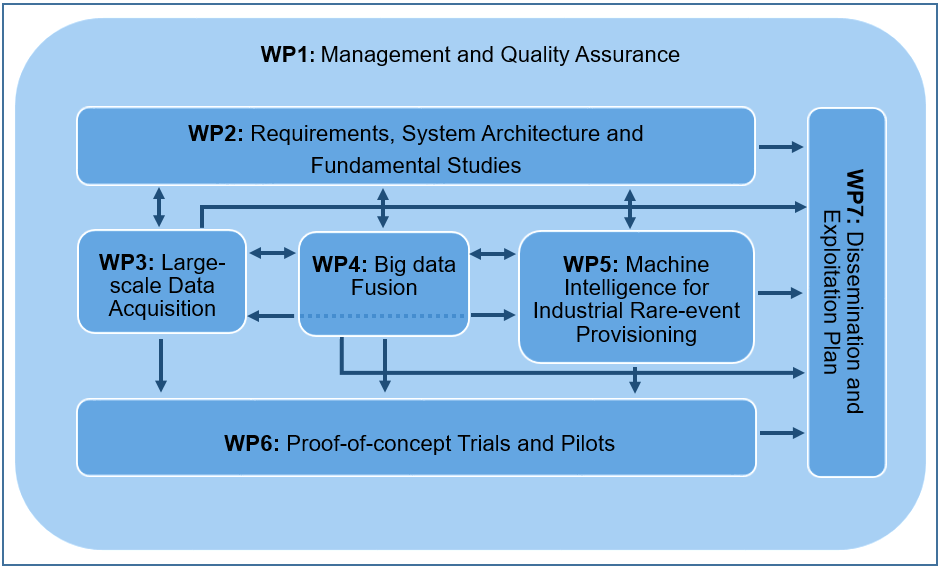
\includegraphics[width=\textwidth]{Images/FIREMAN_pert_diagram.png}
    \caption{FIREMAN WP Diagram \parencite{fireman-homepage}}
    \label{fig:wp-diagram}
\end{figure}

This work focuses on WP6 discussed in Section \ref{ref_wp6} by demonstrating an implementation of a theoretical algorithm for real-world anomaly detection.

\subsubsection{Large Scale Data Acquisition (WP3)}

This work package focuses on \enquote{event-based modelling and traffic characterization techniques aiming for a reduced use of communication and storage resources. This pre-processing task is expected -among others- to optimize the subsequent data transmissions by injecting only relevant data in the network to reduce overhead and increase spectral efficiency.} \citel{wp3.1}

In this portion of FIREMAN, we examined a  variety of industrial datasets including the Tennessee Eastman Process, Electricity Metering, IEC-61850 Distribution Automation, and the EPFL Smart Grid Pilot. This dataset is not heavily reliant on relational constraints or atomicity, consistency, isolation, durability (ACID) compliance. Because of this, we have selected a non-relational PostgreSQL database for storage because of its superior throughput and increased performance in data processing applications.

The sensors traditionally used in Cyber-Physical Systems do not have much compute or storage capacity which makes pre-processing of data at the sensor level challenging. Because of this, \enquote{compression is essential for reducing the challenge of data storage, collection, transmission, processing, and analysis at the local level}\parencite{compression}. Authors \cite{wp3.2} have shown that it is possible to achieve a 92.6\% compression rate which means that only 7.4\% of samples are transmitted. We have also used different methods including linear interpolation to de-compress the data and have measured the error using the root mean square technique.

% \begin{figure}[H]
%     % \centering
%     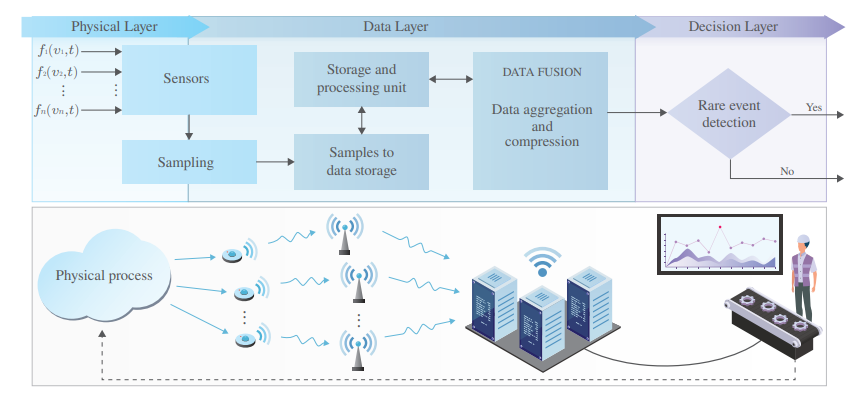
\includegraphics[width=\textwidth]{Images/three-layer-system.PNG}
%     \caption{Three layer framework for rare event detection \parencite{three-layer-approach}}
%     \label{fig:three-layer}
% \end{figure}

Modeling of transmission reduction techniques centered around the electricity modeling dataset \parencite{elect-model-dataset-9694611}. Three approaches for reducing transmissions were presented including transmission on large spikes, transmissions on accumulated variance, and time interval defined transmission with a timeout to compensate for meter or network failure. These simulations have shown a large potential for reducing transmissions without significantly affecting the accuracy of the measured signal. We modeled a Markov-Modulated Poission Process to simulate these industrial processes for use in further stages of the project.

\subsubsection{Big Data Fusion (WP4)}
\label{ref_wp4}
The goal of this task is \enquote{to show how a large number of sensors and their corresponding data can be  accommodated and aggregated at small cost for reliably detecting rare events}\parencite{wp4.1}. This task focuses on three primary objects:
\begin{inlinelist}
    \item heterogeneous data aggregation in machine-type communications;
    \item signature-based cluster formation; and
    \item IoT platform and database selection.
\end{inlinelist}

It is challenging to simultaneously connect a massive number of devices which is why data aggregation is important.
This strategy outlined by Authors \cite{massive-machine} relies on the following principals:
\begin{inlinelist}
  \item decreasing communication distance and power consumption of connected devices;
  \item utilizing an efficient distributed node routing network to decrease bandwidth congestion of central nodes; and
  \item extending the network coverage.
\end{inlinelist}
The researchers also introduced a cluster formation scheme based on signatures that reduces the signalling overhead required for peer-discovery in the network. This technique utilizes signal aggregates to reduce traffic congestion to the central node.

Additionally we surveyed IoT experts to determine the most important properties and components of an IoT system. This survey compared the five most popular cloud IoT providers: AWS, Azure, GCP, IBM Watson, and Oracle IoT to create a comparison that can be used by businesses when selecting a cloud provider that suits their business needs \parencite{choose-iot-9110590}.

SEAT, an automotive component manufacturer, provided two use cases and accompanying datasets for the FIREMAN project. The first involves early failure detection of mechanical components in the drive chain in the Paint shop which causes axial displacement. The second involves detecting early failure of the spindle on a CNC machine which ensures lineal movement over a surface. In both of these situations detecting failure early helps SEAT detect problems and solve them before they begin to impact production components and eventually reduce production downtime to zero.

\subsubsection{Machine Intelligence for Industrial Rare-event Provisioning (WP5)}

The goal of this task is to utilize machine intelligence techniques to predict indicators of health for a machine, component, or entire industrial process to determine health and detect premature failure. The main technique proposed in this task is Quantitative Association Rule Mining Algorithm (QARMA).

\enquote{QARMA is a family of algorithms for extracting all (or, depending on user inputs, an important subset of) valid non-dominated quantitative association rules that hold in a dataset, that can then be used for further data analysis such as deriving rule-based classifier ensembles or as explainers of classification results of other black-box classifiers.}\citel{wp5.1}  This technique is one of the most human understandable techniques for machine intelligence and has shown promise for this application. In this WP, QARMA is tested on the SEAT dataset discussed in Section \ref{ref_wp4}.

Traditional methods for pruning the rules created by the algorithm were analyzed in this WP as many of them can be extraneous or unreliable. The fastest open source Mixed-Integer Programming (MIP) tool was able to solve this problem in 19 seconds while the parallelized hybrid search algorithm proposed in this WP solved the problem 240 times faster when using parallel threads.

Authors \cite{wp5.1} used a breadth first search approach to compute a `small' subset of rules that cover the majority of instances in a training dataset covered by the totality of rules extracted by QARMA applied on it. Through experimentation on a synthetic power grid fault diagnostic dataset QARMA performs better than certain neural networks with noisy data \parencite{ml-performance-power-trans}. This is because of the over-fitting of training data with Deep Neural Network architectures. The rule based methods generated by QARMA produce human understandable rules which is beneficial in creating explainable AI.

\subsubsection{Proof-of-Concept Trails and Pilots (WP6)}
\label{ref_wp6}

The primary objectives of this task as stated by Authors \parencite{wp6.1} using FIREMAN approaches are:
\begin{inlinelist}
    \item testing and deployment of theoretical techniques presented thus far;
    \item specific proof-of-concept demonstrations and simulations ; and
    \item implementation plans for production, real-time monitoring.
\end{inlinelist}

Authors \parencite{wp6.3} describe the Power Electronic Converter (PEC) setup at Aalborg University (AAU) that is discussed in this work. The test setup facilities studying microgrids and the impact of disturbances or faults on power transmission and reliability. With the test setup, it is possible to perturb system parameters and measure their impact on the overall system with various sensor measurements. These simulation conditions are used to create the PEC dataset discussed in Section \ref{ref_pec_dataset}.

\subsection{Algorithm Explainability}

Certain high-risk use cases for machine learning algorithms demand a high level of explainability and confidence in the algorithm outputs to use in fields of decision making. In many cases an algorithm makes a classification decision but there is not a clear explanation as to why the algorithm made that decision. In the field of power electronics, understanding why a data-driven controller is making a decision is critical to incorporating it into real world power distribution scenarios.

Answering these questions is complex and there are a few approaches to achieving this goal. Authors \cite{black-box-explainability} propose using conditional entropy to determine how each input is related to each output. The generated plots are then compared to the physical insights of the system and outlier, adversarial data that falls outside the plot is identified and removed. The model is then retrained. This technique is helpful for identifying and removing adversarial data that falls outside the range of accepted values but it would not identify data overloading in a specific portion of the graph which would create an incorrect classification.

\subsubsection{Types of Uncertainty}
It is often necessary to determine sources of uncertainty in a model or system. When analyzing uncertainty, it is important to understand the two types:
\begin{inlinelist}
    \item epistemic and
    \item aleatoric uncertainty.
\end{inlinelist}

Epistemic uncertainty results from inadequate training data. With this type, the training data is not sufficient to provide enough or accurate date to the model. This can be a result of unbalanced or lack of training data. Increasing the amount of training data or decreasing class imbalance can help reduce this type of uncertainty.

Aleatoric uncertainty arise from probabilistic errors in sampling that follow a specific probability distribution. This type of uncertainty is independent to the amount of data collected and therefore cannot be corrected with more training data. If a signal has noise inline with a given probability distribution, having more data on that signal does not change the noise probability distribution. This type of uncertainty references the distribution of random errors in the data and not the data distribution itself.

For illustration, suppose someone is recording audio at a train station. There are three announcements each hour that disrupt the recording but you do not know when in the hour they occur. Having more data (hours), does not change the amount of announcements that occur.

\subsection{Combating Model Uncertainty}

With deep learning algorithms, it is important to know the level of confidence the model is predicting the outcome with. Authors \cite{explaining-adversarial-examples} explain that adding simple adversarial data (like small noise to a photo) makes an image recognition algorithm incorrectly classify one animal as a completely different one. This is further concerning since adversarial data does not need to be tailored to a specific algorithm. The transferability of this type of adversarial data allows it to be applied to many black box algorithms to achieve an unintended or potentially malicious result.

A malfunctioning sensor or bad connection can generate noise (a type of aleatoric uncertainty), which cannot be fixed by more measurements or more data. Data imputation can be used as a technique to correct for or understand this type of uncertainty. If you can identify that the uncertainty is present, then you can use data imputation to form a well educated guess as to what the value should actually be. The significance of identifying it as aleatoric uncertainty is that no amount of model tuning or data collection can fix the underlying issue, so data imputation presents an opportunity to move forward that standard techniques would not.

\subsubsection{Bayesian Dropout}

Bayesian techniques can be used to create a probability distribution over the weights to determine a level of uncertainty for the weights of each neuron. Authors \cite{bayesian-weight-uncertainty-neural-networks} introduce a standard Bayesian neural network implementation with back-propagation that can determine these probability distributions.

This method is effective at improving model accuracy but Authors \cite{gal2016dropout} explain that retraining a large number of models on a variety of datasets is computationally expensive and time consuming. A dropout technique can be used to approximate the Bayesian representation with significantly less computational cost. Authors \cite{gal2016dropout} explain that this technique avoids over-fitting by randomly sampling and dropping network nodes across many different training iterations.

It is important to perform the dropout technique while training and testing the algorithm and then compute the variance to determine the uncertainty. This enables researchers to determine that for specific values the algorithm is providing a best guess answer with high levels of uncertainty, which could then signal the need for human intervention or review in decision making.

\subsubsection{Shapely Additive Explanations (SHAP)}

Using reverse engineering, the output of a machine learning algorithm can be analyzed and explained. Authors \cite{SHAP-og-paper} introduce \textbf{SH}apely \textbf{A}dditive ex\textbf{P}lanations (SHAP) to interpret and explain the \textit{why} behind machine learning algorithm results.

Machine learning models usually output the likelihood of a certain prediction given a set of inputs, but SHAP explains why the model made that classification decision. SHAP determines how significantly each input contributes to the output of the model by analyzing every possible combination of input weights.

While this technique yields accurate explanations of black-box machine learning outputs, it is still a reverse-engineering technique. It cannot explain a model that is not yet trained and where the outputs are not known. This is problematic for unsupervised or online techniques where the model is created and retrained as new data inputs enter the pipeline. As the model is updated, the decision making parameters that affect the output change and the output looses explainability.

This demonstrates the importance of explainability in unsupervised learning or with techniques that do not have traditional models. In this case, it is important to have an explainable set of rules or behaviors that govern the model \textit{a priori}. This type of model cannot be reverse-engineered since the inputs are constantly updating the model and explanations from reverse-engineering would only be valid for the present iteration and not generalizeable to subsequent predictions.

\subsection{Outlier Taxonomy}

The term `outlier' or `anomaly' can have a variety of interpretations and meanings depending on the context. In order to select and evaluate appropriate techniques for outlier detection, it is essential to understand and define the various types of outliers that can be present in a dataset. Outliers are primarily categorized as:
\begin{inlinelist}
    \item point-wise and
    \item context-wise.
\end{inlinelist}
These distinction between these two types is illustrated graphically in Figure \ref{fig:outliers-graphic}.

% \begin{figure}[H]
%     % \centering
%     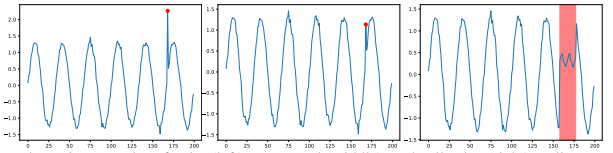
\includegraphics[width=\textwidth]{Images/outliers_graphic.PNG}
%     \caption{[Point, Contextual, and Collective] Outliers \parencite{lai2021revisiting}}
%     \label{fig:outliers-graphic}
% \end{figure}

\begin{figure}[H]
     \centering
     \begin{subfigure}[b]{0.475\textwidth}
         \centering
         {\resizebox{\textwidth}{!}{%% Creator: Matplotlib, PGF backend
%%
%% To include the figure in your LaTeX document, write
%%   \input{<filename>.pgf}
%%
%% Make sure the required packages are loaded in your preamble
%%   \usepackage{pgf}
%%
%% Also ensure that all the required font packages are loaded; for instance,
%% the lmodern package is sometimes necessary when using math font.
%%   \usepackage{lmodern}
%%
%% Figures using additional raster images can only be included by \input if
%% they are in the same directory as the main LaTeX file. For loading figures
%% from other directories you can use the `import` package
%%   \usepackage{import}
%%
%% and then include the figures with
%%   \import{<path to file>}{<filename>.pgf}
%%
%% Matplotlib used the following preamble
%%
\begingroup%
\makeatletter%
\begin{pgfpicture}%
\pgfpathrectangle{\pgfpointorigin}{\pgfqpoint{5.000000in}{4.000000in}}%
\pgfusepath{use as bounding box, clip}%
\begin{pgfscope}%
\pgfsetbuttcap%
\pgfsetmiterjoin%
\pgfsetlinewidth{0.000000pt}%
\definecolor{currentstroke}{rgb}{1.000000,1.000000,1.000000}%
\pgfsetstrokecolor{currentstroke}%
\pgfsetstrokeopacity{0.000000}%
\pgfsetdash{}{0pt}%
\pgfpathmoveto{\pgfqpoint{0.000000in}{0.000000in}}%
\pgfpathlineto{\pgfqpoint{5.000000in}{0.000000in}}%
\pgfpathlineto{\pgfqpoint{5.000000in}{4.000000in}}%
\pgfpathlineto{\pgfqpoint{0.000000in}{4.000000in}}%
\pgfpathlineto{\pgfqpoint{0.000000in}{0.000000in}}%
\pgfpathclose%
\pgfusepath{}%
\end{pgfscope}%
\begin{pgfscope}%
\pgfsetbuttcap%
\pgfsetmiterjoin%
\definecolor{currentfill}{rgb}{1.000000,1.000000,1.000000}%
\pgfsetfillcolor{currentfill}%
\pgfsetlinewidth{0.000000pt}%
\definecolor{currentstroke}{rgb}{0.000000,0.000000,0.000000}%
\pgfsetstrokecolor{currentstroke}%
\pgfsetstrokeopacity{0.000000}%
\pgfsetdash{}{0pt}%
\pgfpathmoveto{\pgfqpoint{0.625000in}{0.500000in}}%
\pgfpathlineto{\pgfqpoint{4.500000in}{0.500000in}}%
\pgfpathlineto{\pgfqpoint{4.500000in}{3.520000in}}%
\pgfpathlineto{\pgfqpoint{0.625000in}{3.520000in}}%
\pgfpathlineto{\pgfqpoint{0.625000in}{0.500000in}}%
\pgfpathclose%
\pgfusepath{fill}%
\end{pgfscope}%
\begin{pgfscope}%
\pgfsetbuttcap%
\pgfsetroundjoin%
\definecolor{currentfill}{rgb}{0.000000,0.000000,0.000000}%
\pgfsetfillcolor{currentfill}%
\pgfsetlinewidth{0.803000pt}%
\definecolor{currentstroke}{rgb}{0.000000,0.000000,0.000000}%
\pgfsetstrokecolor{currentstroke}%
\pgfsetdash{}{0pt}%
\pgfsys@defobject{currentmarker}{\pgfqpoint{0.000000in}{-0.048611in}}{\pgfqpoint{0.000000in}{0.000000in}}{%
\pgfpathmoveto{\pgfqpoint{0.000000in}{0.000000in}}%
\pgfpathlineto{\pgfqpoint{0.000000in}{-0.048611in}}%
\pgfusepath{stroke,fill}%
}%
\begin{pgfscope}%
\pgfsys@transformshift{0.801136in}{0.500000in}%
\pgfsys@useobject{currentmarker}{}%
\end{pgfscope}%
\end{pgfscope}%
\begin{pgfscope}%
\definecolor{textcolor}{rgb}{0.000000,0.000000,0.000000}%
\pgfsetstrokecolor{textcolor}%
\pgfsetfillcolor{textcolor}%
\pgftext[x=0.801136in,y=0.402778in,,top]{\color{textcolor}\rmfamily\fontsize{10.000000}{12.000000}\selectfont \(\displaystyle {0}\)}%
\end{pgfscope}%
\begin{pgfscope}%
\pgfsetbuttcap%
\pgfsetroundjoin%
\definecolor{currentfill}{rgb}{0.000000,0.000000,0.000000}%
\pgfsetfillcolor{currentfill}%
\pgfsetlinewidth{0.803000pt}%
\definecolor{currentstroke}{rgb}{0.000000,0.000000,0.000000}%
\pgfsetstrokecolor{currentstroke}%
\pgfsetdash{}{0pt}%
\pgfsys@defobject{currentmarker}{\pgfqpoint{0.000000in}{-0.048611in}}{\pgfqpoint{0.000000in}{0.000000in}}{%
\pgfpathmoveto{\pgfqpoint{0.000000in}{0.000000in}}%
\pgfpathlineto{\pgfqpoint{0.000000in}{-0.048611in}}%
\pgfusepath{stroke,fill}%
}%
\begin{pgfscope}%
\pgfsys@transformshift{1.506387in}{0.500000in}%
\pgfsys@useobject{currentmarker}{}%
\end{pgfscope}%
\end{pgfscope}%
\begin{pgfscope}%
\definecolor{textcolor}{rgb}{0.000000,0.000000,0.000000}%
\pgfsetstrokecolor{textcolor}%
\pgfsetfillcolor{textcolor}%
\pgftext[x=1.506387in,y=0.402778in,,top]{\color{textcolor}\rmfamily\fontsize{10.000000}{12.000000}\selectfont \(\displaystyle {200}\)}%
\end{pgfscope}%
\begin{pgfscope}%
\pgfsetbuttcap%
\pgfsetroundjoin%
\definecolor{currentfill}{rgb}{0.000000,0.000000,0.000000}%
\pgfsetfillcolor{currentfill}%
\pgfsetlinewidth{0.803000pt}%
\definecolor{currentstroke}{rgb}{0.000000,0.000000,0.000000}%
\pgfsetstrokecolor{currentstroke}%
\pgfsetdash{}{0pt}%
\pgfsys@defobject{currentmarker}{\pgfqpoint{0.000000in}{-0.048611in}}{\pgfqpoint{0.000000in}{0.000000in}}{%
\pgfpathmoveto{\pgfqpoint{0.000000in}{0.000000in}}%
\pgfpathlineto{\pgfqpoint{0.000000in}{-0.048611in}}%
\pgfusepath{stroke,fill}%
}%
\begin{pgfscope}%
\pgfsys@transformshift{2.211638in}{0.500000in}%
\pgfsys@useobject{currentmarker}{}%
\end{pgfscope}%
\end{pgfscope}%
\begin{pgfscope}%
\definecolor{textcolor}{rgb}{0.000000,0.000000,0.000000}%
\pgfsetstrokecolor{textcolor}%
\pgfsetfillcolor{textcolor}%
\pgftext[x=2.211638in,y=0.402778in,,top]{\color{textcolor}\rmfamily\fontsize{10.000000}{12.000000}\selectfont \(\displaystyle {400}\)}%
\end{pgfscope}%
\begin{pgfscope}%
\pgfsetbuttcap%
\pgfsetroundjoin%
\definecolor{currentfill}{rgb}{0.000000,0.000000,0.000000}%
\pgfsetfillcolor{currentfill}%
\pgfsetlinewidth{0.803000pt}%
\definecolor{currentstroke}{rgb}{0.000000,0.000000,0.000000}%
\pgfsetstrokecolor{currentstroke}%
\pgfsetdash{}{0pt}%
\pgfsys@defobject{currentmarker}{\pgfqpoint{0.000000in}{-0.048611in}}{\pgfqpoint{0.000000in}{0.000000in}}{%
\pgfpathmoveto{\pgfqpoint{0.000000in}{0.000000in}}%
\pgfpathlineto{\pgfqpoint{0.000000in}{-0.048611in}}%
\pgfusepath{stroke,fill}%
}%
\begin{pgfscope}%
\pgfsys@transformshift{2.916888in}{0.500000in}%
\pgfsys@useobject{currentmarker}{}%
\end{pgfscope}%
\end{pgfscope}%
\begin{pgfscope}%
\definecolor{textcolor}{rgb}{0.000000,0.000000,0.000000}%
\pgfsetstrokecolor{textcolor}%
\pgfsetfillcolor{textcolor}%
\pgftext[x=2.916888in,y=0.402778in,,top]{\color{textcolor}\rmfamily\fontsize{10.000000}{12.000000}\selectfont \(\displaystyle {600}\)}%
\end{pgfscope}%
\begin{pgfscope}%
\pgfsetbuttcap%
\pgfsetroundjoin%
\definecolor{currentfill}{rgb}{0.000000,0.000000,0.000000}%
\pgfsetfillcolor{currentfill}%
\pgfsetlinewidth{0.803000pt}%
\definecolor{currentstroke}{rgb}{0.000000,0.000000,0.000000}%
\pgfsetstrokecolor{currentstroke}%
\pgfsetdash{}{0pt}%
\pgfsys@defobject{currentmarker}{\pgfqpoint{0.000000in}{-0.048611in}}{\pgfqpoint{0.000000in}{0.000000in}}{%
\pgfpathmoveto{\pgfqpoint{0.000000in}{0.000000in}}%
\pgfpathlineto{\pgfqpoint{0.000000in}{-0.048611in}}%
\pgfusepath{stroke,fill}%
}%
\begin{pgfscope}%
\pgfsys@transformshift{3.622139in}{0.500000in}%
\pgfsys@useobject{currentmarker}{}%
\end{pgfscope}%
\end{pgfscope}%
\begin{pgfscope}%
\definecolor{textcolor}{rgb}{0.000000,0.000000,0.000000}%
\pgfsetstrokecolor{textcolor}%
\pgfsetfillcolor{textcolor}%
\pgftext[x=3.622139in,y=0.402778in,,top]{\color{textcolor}\rmfamily\fontsize{10.000000}{12.000000}\selectfont \(\displaystyle {800}\)}%
\end{pgfscope}%
\begin{pgfscope}%
\pgfsetbuttcap%
\pgfsetroundjoin%
\definecolor{currentfill}{rgb}{0.000000,0.000000,0.000000}%
\pgfsetfillcolor{currentfill}%
\pgfsetlinewidth{0.803000pt}%
\definecolor{currentstroke}{rgb}{0.000000,0.000000,0.000000}%
\pgfsetstrokecolor{currentstroke}%
\pgfsetdash{}{0pt}%
\pgfsys@defobject{currentmarker}{\pgfqpoint{0.000000in}{-0.048611in}}{\pgfqpoint{0.000000in}{0.000000in}}{%
\pgfpathmoveto{\pgfqpoint{0.000000in}{0.000000in}}%
\pgfpathlineto{\pgfqpoint{0.000000in}{-0.048611in}}%
\pgfusepath{stroke,fill}%
}%
\begin{pgfscope}%
\pgfsys@transformshift{4.327390in}{0.500000in}%
\pgfsys@useobject{currentmarker}{}%
\end{pgfscope}%
\end{pgfscope}%
\begin{pgfscope}%
\definecolor{textcolor}{rgb}{0.000000,0.000000,0.000000}%
\pgfsetstrokecolor{textcolor}%
\pgfsetfillcolor{textcolor}%
\pgftext[x=4.327390in,y=0.402778in,,top]{\color{textcolor}\rmfamily\fontsize{10.000000}{12.000000}\selectfont \(\displaystyle {1000}\)}%
\end{pgfscope}%
\begin{pgfscope}%
\definecolor{textcolor}{rgb}{0.000000,0.000000,0.000000}%
\pgfsetstrokecolor{textcolor}%
\pgfsetfillcolor{textcolor}%
\pgftext[x=2.562500in,y=0.223766in,,top]{\color{textcolor}\rmfamily\fontsize{10.000000}{12.000000}\selectfont Sample (n)}%
\end{pgfscope}%
\begin{pgfscope}%
\pgfsetbuttcap%
\pgfsetroundjoin%
\definecolor{currentfill}{rgb}{0.000000,0.000000,0.000000}%
\pgfsetfillcolor{currentfill}%
\pgfsetlinewidth{0.803000pt}%
\definecolor{currentstroke}{rgb}{0.000000,0.000000,0.000000}%
\pgfsetstrokecolor{currentstroke}%
\pgfsetdash{}{0pt}%
\pgfsys@defobject{currentmarker}{\pgfqpoint{-0.048611in}{0.000000in}}{\pgfqpoint{-0.000000in}{0.000000in}}{%
\pgfpathmoveto{\pgfqpoint{-0.000000in}{0.000000in}}%
\pgfpathlineto{\pgfqpoint{-0.048611in}{0.000000in}}%
\pgfusepath{stroke,fill}%
}%
\begin{pgfscope}%
\pgfsys@transformshift{0.625000in}{0.637273in}%
\pgfsys@useobject{currentmarker}{}%
\end{pgfscope}%
\end{pgfscope}%
\begin{pgfscope}%
\definecolor{textcolor}{rgb}{0.000000,0.000000,0.000000}%
\pgfsetstrokecolor{textcolor}%
\pgfsetfillcolor{textcolor}%
\pgftext[x=0.242283in, y=0.589047in, left, base]{\color{textcolor}\rmfamily\fontsize{10.000000}{12.000000}\selectfont \(\displaystyle {\ensuremath{-}1.0}\)}%
\end{pgfscope}%
\begin{pgfscope}%
\pgfsetbuttcap%
\pgfsetroundjoin%
\definecolor{currentfill}{rgb}{0.000000,0.000000,0.000000}%
\pgfsetfillcolor{currentfill}%
\pgfsetlinewidth{0.803000pt}%
\definecolor{currentstroke}{rgb}{0.000000,0.000000,0.000000}%
\pgfsetstrokecolor{currentstroke}%
\pgfsetdash{}{0pt}%
\pgfsys@defobject{currentmarker}{\pgfqpoint{-0.048611in}{0.000000in}}{\pgfqpoint{-0.000000in}{0.000000in}}{%
\pgfpathmoveto{\pgfqpoint{-0.000000in}{0.000000in}}%
\pgfpathlineto{\pgfqpoint{-0.048611in}{0.000000in}}%
\pgfusepath{stroke,fill}%
}%
\begin{pgfscope}%
\pgfsys@transformshift{0.625000in}{1.094848in}%
\pgfsys@useobject{currentmarker}{}%
\end{pgfscope}%
\end{pgfscope}%
\begin{pgfscope}%
\definecolor{textcolor}{rgb}{0.000000,0.000000,0.000000}%
\pgfsetstrokecolor{textcolor}%
\pgfsetfillcolor{textcolor}%
\pgftext[x=0.242283in, y=1.046623in, left, base]{\color{textcolor}\rmfamily\fontsize{10.000000}{12.000000}\selectfont \(\displaystyle {\ensuremath{-}0.5}\)}%
\end{pgfscope}%
\begin{pgfscope}%
\pgfsetbuttcap%
\pgfsetroundjoin%
\definecolor{currentfill}{rgb}{0.000000,0.000000,0.000000}%
\pgfsetfillcolor{currentfill}%
\pgfsetlinewidth{0.803000pt}%
\definecolor{currentstroke}{rgb}{0.000000,0.000000,0.000000}%
\pgfsetstrokecolor{currentstroke}%
\pgfsetdash{}{0pt}%
\pgfsys@defobject{currentmarker}{\pgfqpoint{-0.048611in}{0.000000in}}{\pgfqpoint{-0.000000in}{0.000000in}}{%
\pgfpathmoveto{\pgfqpoint{-0.000000in}{0.000000in}}%
\pgfpathlineto{\pgfqpoint{-0.048611in}{0.000000in}}%
\pgfusepath{stroke,fill}%
}%
\begin{pgfscope}%
\pgfsys@transformshift{0.625000in}{1.552424in}%
\pgfsys@useobject{currentmarker}{}%
\end{pgfscope}%
\end{pgfscope}%
\begin{pgfscope}%
\definecolor{textcolor}{rgb}{0.000000,0.000000,0.000000}%
\pgfsetstrokecolor{textcolor}%
\pgfsetfillcolor{textcolor}%
\pgftext[x=0.350308in, y=1.504199in, left, base]{\color{textcolor}\rmfamily\fontsize{10.000000}{12.000000}\selectfont \(\displaystyle {0.0}\)}%
\end{pgfscope}%
\begin{pgfscope}%
\pgfsetbuttcap%
\pgfsetroundjoin%
\definecolor{currentfill}{rgb}{0.000000,0.000000,0.000000}%
\pgfsetfillcolor{currentfill}%
\pgfsetlinewidth{0.803000pt}%
\definecolor{currentstroke}{rgb}{0.000000,0.000000,0.000000}%
\pgfsetstrokecolor{currentstroke}%
\pgfsetdash{}{0pt}%
\pgfsys@defobject{currentmarker}{\pgfqpoint{-0.048611in}{0.000000in}}{\pgfqpoint{-0.000000in}{0.000000in}}{%
\pgfpathmoveto{\pgfqpoint{-0.000000in}{0.000000in}}%
\pgfpathlineto{\pgfqpoint{-0.048611in}{0.000000in}}%
\pgfusepath{stroke,fill}%
}%
\begin{pgfscope}%
\pgfsys@transformshift{0.625000in}{2.010000in}%
\pgfsys@useobject{currentmarker}{}%
\end{pgfscope}%
\end{pgfscope}%
\begin{pgfscope}%
\definecolor{textcolor}{rgb}{0.000000,0.000000,0.000000}%
\pgfsetstrokecolor{textcolor}%
\pgfsetfillcolor{textcolor}%
\pgftext[x=0.350308in, y=1.961775in, left, base]{\color{textcolor}\rmfamily\fontsize{10.000000}{12.000000}\selectfont \(\displaystyle {0.5}\)}%
\end{pgfscope}%
\begin{pgfscope}%
\pgfsetbuttcap%
\pgfsetroundjoin%
\definecolor{currentfill}{rgb}{0.000000,0.000000,0.000000}%
\pgfsetfillcolor{currentfill}%
\pgfsetlinewidth{0.803000pt}%
\definecolor{currentstroke}{rgb}{0.000000,0.000000,0.000000}%
\pgfsetstrokecolor{currentstroke}%
\pgfsetdash{}{0pt}%
\pgfsys@defobject{currentmarker}{\pgfqpoint{-0.048611in}{0.000000in}}{\pgfqpoint{-0.000000in}{0.000000in}}{%
\pgfpathmoveto{\pgfqpoint{-0.000000in}{0.000000in}}%
\pgfpathlineto{\pgfqpoint{-0.048611in}{0.000000in}}%
\pgfusepath{stroke,fill}%
}%
\begin{pgfscope}%
\pgfsys@transformshift{0.625000in}{2.467576in}%
\pgfsys@useobject{currentmarker}{}%
\end{pgfscope}%
\end{pgfscope}%
\begin{pgfscope}%
\definecolor{textcolor}{rgb}{0.000000,0.000000,0.000000}%
\pgfsetstrokecolor{textcolor}%
\pgfsetfillcolor{textcolor}%
\pgftext[x=0.350308in, y=2.419350in, left, base]{\color{textcolor}\rmfamily\fontsize{10.000000}{12.000000}\selectfont \(\displaystyle {1.0}\)}%
\end{pgfscope}%
\begin{pgfscope}%
\pgfsetbuttcap%
\pgfsetroundjoin%
\definecolor{currentfill}{rgb}{0.000000,0.000000,0.000000}%
\pgfsetfillcolor{currentfill}%
\pgfsetlinewidth{0.803000pt}%
\definecolor{currentstroke}{rgb}{0.000000,0.000000,0.000000}%
\pgfsetstrokecolor{currentstroke}%
\pgfsetdash{}{0pt}%
\pgfsys@defobject{currentmarker}{\pgfqpoint{-0.048611in}{0.000000in}}{\pgfqpoint{-0.000000in}{0.000000in}}{%
\pgfpathmoveto{\pgfqpoint{-0.000000in}{0.000000in}}%
\pgfpathlineto{\pgfqpoint{-0.048611in}{0.000000in}}%
\pgfusepath{stroke,fill}%
}%
\begin{pgfscope}%
\pgfsys@transformshift{0.625000in}{2.925152in}%
\pgfsys@useobject{currentmarker}{}%
\end{pgfscope}%
\end{pgfscope}%
\begin{pgfscope}%
\definecolor{textcolor}{rgb}{0.000000,0.000000,0.000000}%
\pgfsetstrokecolor{textcolor}%
\pgfsetfillcolor{textcolor}%
\pgftext[x=0.350308in, y=2.876926in, left, base]{\color{textcolor}\rmfamily\fontsize{10.000000}{12.000000}\selectfont \(\displaystyle {1.5}\)}%
\end{pgfscope}%
\begin{pgfscope}%
\pgfsetbuttcap%
\pgfsetroundjoin%
\definecolor{currentfill}{rgb}{0.000000,0.000000,0.000000}%
\pgfsetfillcolor{currentfill}%
\pgfsetlinewidth{0.803000pt}%
\definecolor{currentstroke}{rgb}{0.000000,0.000000,0.000000}%
\pgfsetstrokecolor{currentstroke}%
\pgfsetdash{}{0pt}%
\pgfsys@defobject{currentmarker}{\pgfqpoint{-0.048611in}{0.000000in}}{\pgfqpoint{-0.000000in}{0.000000in}}{%
\pgfpathmoveto{\pgfqpoint{-0.000000in}{0.000000in}}%
\pgfpathlineto{\pgfqpoint{-0.048611in}{0.000000in}}%
\pgfusepath{stroke,fill}%
}%
\begin{pgfscope}%
\pgfsys@transformshift{0.625000in}{3.382727in}%
\pgfsys@useobject{currentmarker}{}%
\end{pgfscope}%
\end{pgfscope}%
\begin{pgfscope}%
\definecolor{textcolor}{rgb}{0.000000,0.000000,0.000000}%
\pgfsetstrokecolor{textcolor}%
\pgfsetfillcolor{textcolor}%
\pgftext[x=0.350308in, y=3.334502in, left, base]{\color{textcolor}\rmfamily\fontsize{10.000000}{12.000000}\selectfont \(\displaystyle {2.0}\)}%
\end{pgfscope}%
\begin{pgfscope}%
\definecolor{textcolor}{rgb}{0.000000,0.000000,0.000000}%
\pgfsetstrokecolor{textcolor}%
\pgfsetfillcolor{textcolor}%
\pgftext[x=0.186727in,y=2.010000in,,bottom,rotate=90.000000]{\color{textcolor}\rmfamily\fontsize{10.000000}{12.000000}\selectfont Voltage (\(\displaystyle V\))}%
\end{pgfscope}%
\begin{pgfscope}%
\pgfpathrectangle{\pgfqpoint{0.625000in}{0.500000in}}{\pgfqpoint{3.875000in}{3.020000in}}%
\pgfusepath{clip}%
\pgfsetrectcap%
\pgfsetroundjoin%
\pgfsetlinewidth{1.505625pt}%
\definecolor{currentstroke}{rgb}{0.121569,0.466667,0.705882}%
\pgfsetstrokecolor{currentstroke}%
\pgfsetdash{}{0pt}%
\pgfpathmoveto{\pgfqpoint{0.801136in}{1.552424in}}%
\pgfpathlineto{\pgfqpoint{0.846978in}{1.915875in}}%
\pgfpathlineto{\pgfqpoint{0.871661in}{2.090337in}}%
\pgfpathlineto{\pgfqpoint{0.892819in}{2.219541in}}%
\pgfpathlineto{\pgfqpoint{0.910450in}{2.309328in}}%
\pgfpathlineto{\pgfqpoint{0.924555in}{2.367830in}}%
\pgfpathlineto{\pgfqpoint{0.938660in}{2.413473in}}%
\pgfpathlineto{\pgfqpoint{0.949239in}{2.438825in}}%
\pgfpathlineto{\pgfqpoint{0.959818in}{2.456309in}}%
\pgfpathlineto{\pgfqpoint{0.966870in}{2.463514in}}%
\pgfpathlineto{\pgfqpoint{0.973923in}{2.467124in}}%
\pgfpathlineto{\pgfqpoint{0.980975in}{2.467124in}}%
\pgfpathlineto{\pgfqpoint{0.988028in}{2.463514in}}%
\pgfpathlineto{\pgfqpoint{0.995080in}{2.456309in}}%
\pgfpathlineto{\pgfqpoint{1.005659in}{2.438825in}}%
\pgfpathlineto{\pgfqpoint{1.016238in}{2.413473in}}%
\pgfpathlineto{\pgfqpoint{1.026817in}{2.380478in}}%
\pgfpathlineto{\pgfqpoint{1.040922in}{2.325112in}}%
\pgfpathlineto{\pgfqpoint{1.055027in}{2.257561in}}%
\pgfpathlineto{\pgfqpoint{1.072658in}{2.157625in}}%
\pgfpathlineto{\pgfqpoint{1.093815in}{2.018274in}}%
\pgfpathlineto{\pgfqpoint{1.122025in}{1.807743in}}%
\pgfpathlineto{\pgfqpoint{1.224287in}{1.014512in}}%
\pgfpathlineto{\pgfqpoint{1.245444in}{0.885307in}}%
\pgfpathlineto{\pgfqpoint{1.263076in}{0.795520in}}%
\pgfpathlineto{\pgfqpoint{1.277181in}{0.737018in}}%
\pgfpathlineto{\pgfqpoint{1.291286in}{0.691376in}}%
\pgfpathlineto{\pgfqpoint{1.301864in}{0.666024in}}%
\pgfpathlineto{\pgfqpoint{1.312443in}{0.648540in}}%
\pgfpathlineto{\pgfqpoint{1.319496in}{0.641334in}}%
\pgfpathlineto{\pgfqpoint{1.326548in}{0.637724in}}%
\pgfpathlineto{\pgfqpoint{1.333601in}{0.637724in}}%
\pgfpathlineto{\pgfqpoint{1.340653in}{0.641334in}}%
\pgfpathlineto{\pgfqpoint{1.347706in}{0.648540in}}%
\pgfpathlineto{\pgfqpoint{1.358284in}{0.666024in}}%
\pgfpathlineto{\pgfqpoint{1.368863in}{0.691376in}}%
\pgfpathlineto{\pgfqpoint{1.379442in}{0.724370in}}%
\pgfpathlineto{\pgfqpoint{1.393547in}{0.779736in}}%
\pgfpathlineto{\pgfqpoint{1.407652in}{0.847288in}}%
\pgfpathlineto{\pgfqpoint{1.425283in}{0.947224in}}%
\pgfpathlineto{\pgfqpoint{1.446441in}{1.086574in}}%
\pgfpathlineto{\pgfqpoint{1.474651in}{1.297105in}}%
\pgfpathlineto{\pgfqpoint{1.576912in}{2.090337in}}%
\pgfpathlineto{\pgfqpoint{1.598070in}{2.219541in}}%
\pgfpathlineto{\pgfqpoint{1.615701in}{2.309328in}}%
\pgfpathlineto{\pgfqpoint{1.629806in}{2.367830in}}%
\pgfpathlineto{\pgfqpoint{1.643911in}{2.413473in}}%
\pgfpathlineto{\pgfqpoint{1.654490in}{2.438825in}}%
\pgfpathlineto{\pgfqpoint{1.665068in}{2.456309in}}%
\pgfpathlineto{\pgfqpoint{1.672121in}{2.463514in}}%
\pgfpathlineto{\pgfqpoint{1.679173in}{2.467124in}}%
\pgfpathlineto{\pgfqpoint{1.686226in}{2.467124in}}%
\pgfpathlineto{\pgfqpoint{1.693279in}{2.463514in}}%
\pgfpathlineto{\pgfqpoint{1.700331in}{2.456309in}}%
\pgfpathlineto{\pgfqpoint{1.710910in}{2.438825in}}%
\pgfpathlineto{\pgfqpoint{1.721489in}{2.413473in}}%
\pgfpathlineto{\pgfqpoint{1.732067in}{2.380478in}}%
\pgfpathlineto{\pgfqpoint{1.746172in}{2.325112in}}%
\pgfpathlineto{\pgfqpoint{1.760277in}{2.257561in}}%
\pgfpathlineto{\pgfqpoint{1.777909in}{2.157625in}}%
\pgfpathlineto{\pgfqpoint{1.799066in}{2.018274in}}%
\pgfpathlineto{\pgfqpoint{1.827276in}{1.807743in}}%
\pgfpathlineto{\pgfqpoint{1.929537in}{1.014512in}}%
\pgfpathlineto{\pgfqpoint{1.950695in}{0.885307in}}%
\pgfpathlineto{\pgfqpoint{1.968326in}{0.795520in}}%
\pgfpathlineto{\pgfqpoint{1.982431in}{0.737018in}}%
\pgfpathlineto{\pgfqpoint{1.996536in}{0.691376in}}%
\pgfpathlineto{\pgfqpoint{2.007115in}{0.666024in}}%
\pgfpathlineto{\pgfqpoint{2.017694in}{0.648540in}}%
\pgfpathlineto{\pgfqpoint{2.024746in}{0.641334in}}%
\pgfpathlineto{\pgfqpoint{2.031799in}{0.637724in}}%
\pgfpathlineto{\pgfqpoint{2.038851in}{0.637724in}}%
\pgfpathlineto{\pgfqpoint{2.045904in}{0.641334in}}%
\pgfpathlineto{\pgfqpoint{2.052956in}{0.648540in}}%
\pgfpathlineto{\pgfqpoint{2.063535in}{0.666024in}}%
\pgfpathlineto{\pgfqpoint{2.074114in}{0.691376in}}%
\pgfpathlineto{\pgfqpoint{2.084693in}{0.724370in}}%
\pgfpathlineto{\pgfqpoint{2.098798in}{0.779736in}}%
\pgfpathlineto{\pgfqpoint{2.112903in}{0.847288in}}%
\pgfpathlineto{\pgfqpoint{2.130534in}{0.947224in}}%
\pgfpathlineto{\pgfqpoint{2.151691in}{1.086574in}}%
\pgfpathlineto{\pgfqpoint{2.179901in}{1.297105in}}%
\pgfpathlineto{\pgfqpoint{2.208112in}{1.523679in}}%
\pgfpathlineto{\pgfqpoint{2.211638in}{3.382727in}}%
\pgfpathlineto{\pgfqpoint{2.215164in}{1.581170in}}%
\pgfpathlineto{\pgfqpoint{2.261005in}{1.942077in}}%
\pgfpathlineto{\pgfqpoint{2.285689in}{2.113327in}}%
\pgfpathlineto{\pgfqpoint{2.306847in}{2.238890in}}%
\pgfpathlineto{\pgfqpoint{2.324478in}{2.325112in}}%
\pgfpathlineto{\pgfqpoint{2.338583in}{2.380478in}}%
\pgfpathlineto{\pgfqpoint{2.352688in}{2.422785in}}%
\pgfpathlineto{\pgfqpoint{2.363267in}{2.445536in}}%
\pgfpathlineto{\pgfqpoint{2.373845in}{2.460360in}}%
\pgfpathlineto{\pgfqpoint{2.380898in}{2.465770in}}%
\pgfpathlineto{\pgfqpoint{2.387950in}{2.467576in}}%
\pgfpathlineto{\pgfqpoint{2.395003in}{2.465770in}}%
\pgfpathlineto{\pgfqpoint{2.402055in}{2.460360in}}%
\pgfpathlineto{\pgfqpoint{2.409108in}{2.451366in}}%
\pgfpathlineto{\pgfqpoint{2.419687in}{2.431238in}}%
\pgfpathlineto{\pgfqpoint{2.430265in}{2.403311in}}%
\pgfpathlineto{\pgfqpoint{2.444371in}{2.354378in}}%
\pgfpathlineto{\pgfqpoint{2.458476in}{2.292797in}}%
\pgfpathlineto{\pgfqpoint{2.476107in}{2.199534in}}%
\pgfpathlineto{\pgfqpoint{2.497264in}{2.066816in}}%
\pgfpathlineto{\pgfqpoint{2.521948in}{1.889314in}}%
\pgfpathlineto{\pgfqpoint{2.557211in}{1.609887in}}%
\pgfpathlineto{\pgfqpoint{2.613631in}{1.162772in}}%
\pgfpathlineto{\pgfqpoint{2.638314in}{0.991521in}}%
\pgfpathlineto{\pgfqpoint{2.659472in}{0.865959in}}%
\pgfpathlineto{\pgfqpoint{2.677103in}{0.779736in}}%
\pgfpathlineto{\pgfqpoint{2.691208in}{0.724370in}}%
\pgfpathlineto{\pgfqpoint{2.705313in}{0.682063in}}%
\pgfpathlineto{\pgfqpoint{2.715892in}{0.659313in}}%
\pgfpathlineto{\pgfqpoint{2.726471in}{0.644489in}}%
\pgfpathlineto{\pgfqpoint{2.733523in}{0.639079in}}%
\pgfpathlineto{\pgfqpoint{2.740576in}{0.637273in}}%
\pgfpathlineto{\pgfqpoint{2.747628in}{0.639079in}}%
\pgfpathlineto{\pgfqpoint{2.754681in}{0.644489in}}%
\pgfpathlineto{\pgfqpoint{2.761733in}{0.653483in}}%
\pgfpathlineto{\pgfqpoint{2.772312in}{0.673610in}}%
\pgfpathlineto{\pgfqpoint{2.782891in}{0.701538in}}%
\pgfpathlineto{\pgfqpoint{2.796996in}{0.750471in}}%
\pgfpathlineto{\pgfqpoint{2.811101in}{0.812051in}}%
\pgfpathlineto{\pgfqpoint{2.828732in}{0.905314in}}%
\pgfpathlineto{\pgfqpoint{2.849890in}{1.038033in}}%
\pgfpathlineto{\pgfqpoint{2.874573in}{1.215535in}}%
\pgfpathlineto{\pgfqpoint{2.909836in}{1.494961in}}%
\pgfpathlineto{\pgfqpoint{2.966256in}{1.942077in}}%
\pgfpathlineto{\pgfqpoint{2.990940in}{2.113327in}}%
\pgfpathlineto{\pgfqpoint{3.012097in}{2.238890in}}%
\pgfpathlineto{\pgfqpoint{3.029729in}{2.325112in}}%
\pgfpathlineto{\pgfqpoint{3.043834in}{2.380478in}}%
\pgfpathlineto{\pgfqpoint{3.057939in}{2.422785in}}%
\pgfpathlineto{\pgfqpoint{3.068517in}{2.445536in}}%
\pgfpathlineto{\pgfqpoint{3.079096in}{2.460360in}}%
\pgfpathlineto{\pgfqpoint{3.086149in}{2.465770in}}%
\pgfpathlineto{\pgfqpoint{3.093201in}{2.467576in}}%
\pgfpathlineto{\pgfqpoint{3.100254in}{2.465770in}}%
\pgfpathlineto{\pgfqpoint{3.107306in}{2.460360in}}%
\pgfpathlineto{\pgfqpoint{3.114359in}{2.451366in}}%
\pgfpathlineto{\pgfqpoint{3.124937in}{2.431238in}}%
\pgfpathlineto{\pgfqpoint{3.135516in}{2.403311in}}%
\pgfpathlineto{\pgfqpoint{3.149621in}{2.354378in}}%
\pgfpathlineto{\pgfqpoint{3.163726in}{2.292797in}}%
\pgfpathlineto{\pgfqpoint{3.181357in}{2.199534in}}%
\pgfpathlineto{\pgfqpoint{3.202515in}{2.066816in}}%
\pgfpathlineto{\pgfqpoint{3.227199in}{1.889314in}}%
\pgfpathlineto{\pgfqpoint{3.262461in}{1.609887in}}%
\pgfpathlineto{\pgfqpoint{3.318881in}{1.162772in}}%
\pgfpathlineto{\pgfqpoint{3.343565in}{0.991521in}}%
\pgfpathlineto{\pgfqpoint{3.364723in}{0.865959in}}%
\pgfpathlineto{\pgfqpoint{3.382354in}{0.779736in}}%
\pgfpathlineto{\pgfqpoint{3.396459in}{0.724370in}}%
\pgfpathlineto{\pgfqpoint{3.410564in}{0.682063in}}%
\pgfpathlineto{\pgfqpoint{3.421143in}{0.659313in}}%
\pgfpathlineto{\pgfqpoint{3.431721in}{0.644489in}}%
\pgfpathlineto{\pgfqpoint{3.438774in}{0.639079in}}%
\pgfpathlineto{\pgfqpoint{3.445827in}{0.637273in}}%
\pgfpathlineto{\pgfqpoint{3.452879in}{0.639079in}}%
\pgfpathlineto{\pgfqpoint{3.459932in}{0.644489in}}%
\pgfpathlineto{\pgfqpoint{3.466984in}{0.653483in}}%
\pgfpathlineto{\pgfqpoint{3.477563in}{0.673610in}}%
\pgfpathlineto{\pgfqpoint{3.488142in}{0.701538in}}%
\pgfpathlineto{\pgfqpoint{3.502247in}{0.750471in}}%
\pgfpathlineto{\pgfqpoint{3.516352in}{0.812051in}}%
\pgfpathlineto{\pgfqpoint{3.533983in}{0.905314in}}%
\pgfpathlineto{\pgfqpoint{3.555140in}{1.038033in}}%
\pgfpathlineto{\pgfqpoint{3.579824in}{1.215535in}}%
\pgfpathlineto{\pgfqpoint{3.615087in}{1.494961in}}%
\pgfpathlineto{\pgfqpoint{3.671507in}{1.942077in}}%
\pgfpathlineto{\pgfqpoint{3.696191in}{2.113327in}}%
\pgfpathlineto{\pgfqpoint{3.717348in}{2.238890in}}%
\pgfpathlineto{\pgfqpoint{3.734979in}{2.325112in}}%
\pgfpathlineto{\pgfqpoint{3.749084in}{2.380478in}}%
\pgfpathlineto{\pgfqpoint{3.763189in}{2.422785in}}%
\pgfpathlineto{\pgfqpoint{3.773768in}{2.445536in}}%
\pgfpathlineto{\pgfqpoint{3.784347in}{2.460360in}}%
\pgfpathlineto{\pgfqpoint{3.791399in}{2.465770in}}%
\pgfpathlineto{\pgfqpoint{3.798452in}{2.467576in}}%
\pgfpathlineto{\pgfqpoint{3.805504in}{2.465770in}}%
\pgfpathlineto{\pgfqpoint{3.812557in}{2.460360in}}%
\pgfpathlineto{\pgfqpoint{3.819609in}{2.451366in}}%
\pgfpathlineto{\pgfqpoint{3.830188in}{2.431238in}}%
\pgfpathlineto{\pgfqpoint{3.840767in}{2.403311in}}%
\pgfpathlineto{\pgfqpoint{3.854872in}{2.354378in}}%
\pgfpathlineto{\pgfqpoint{3.868977in}{2.292797in}}%
\pgfpathlineto{\pgfqpoint{3.886608in}{2.199534in}}%
\pgfpathlineto{\pgfqpoint{3.907766in}{2.066816in}}%
\pgfpathlineto{\pgfqpoint{3.932449in}{1.889314in}}%
\pgfpathlineto{\pgfqpoint{3.967712in}{1.609887in}}%
\pgfpathlineto{\pgfqpoint{4.024132in}{1.162772in}}%
\pgfpathlineto{\pgfqpoint{4.048816in}{0.991521in}}%
\pgfpathlineto{\pgfqpoint{4.069973in}{0.865959in}}%
\pgfpathlineto{\pgfqpoint{4.087605in}{0.779736in}}%
\pgfpathlineto{\pgfqpoint{4.101710in}{0.724370in}}%
\pgfpathlineto{\pgfqpoint{4.115815in}{0.682063in}}%
\pgfpathlineto{\pgfqpoint{4.126393in}{0.659313in}}%
\pgfpathlineto{\pgfqpoint{4.136972in}{0.644489in}}%
\pgfpathlineto{\pgfqpoint{4.144025in}{0.639079in}}%
\pgfpathlineto{\pgfqpoint{4.151077in}{0.637273in}}%
\pgfpathlineto{\pgfqpoint{4.158130in}{0.639079in}}%
\pgfpathlineto{\pgfqpoint{4.165182in}{0.644489in}}%
\pgfpathlineto{\pgfqpoint{4.172235in}{0.653483in}}%
\pgfpathlineto{\pgfqpoint{4.182813in}{0.673610in}}%
\pgfpathlineto{\pgfqpoint{4.193392in}{0.701538in}}%
\pgfpathlineto{\pgfqpoint{4.207497in}{0.750471in}}%
\pgfpathlineto{\pgfqpoint{4.221602in}{0.812051in}}%
\pgfpathlineto{\pgfqpoint{4.239234in}{0.905314in}}%
\pgfpathlineto{\pgfqpoint{4.260391in}{1.038033in}}%
\pgfpathlineto{\pgfqpoint{4.285075in}{1.215535in}}%
\pgfpathlineto{\pgfqpoint{4.320337in}{1.494961in}}%
\pgfpathlineto{\pgfqpoint{4.323864in}{1.523679in}}%
\pgfpathlineto{\pgfqpoint{4.323864in}{1.523679in}}%
\pgfusepath{stroke}%
\end{pgfscope}%
\begin{pgfscope}%
\pgfpathrectangle{\pgfqpoint{0.625000in}{0.500000in}}{\pgfqpoint{3.875000in}{3.020000in}}%
\pgfusepath{clip}%
\pgfsetbuttcap%
\pgfsetroundjoin%
\definecolor{currentfill}{rgb}{1.000000,0.000000,0.000000}%
\pgfsetfillcolor{currentfill}%
\pgfsetlinewidth{1.003750pt}%
\definecolor{currentstroke}{rgb}{1.000000,0.000000,0.000000}%
\pgfsetstrokecolor{currentstroke}%
\pgfsetdash{}{0pt}%
\pgfsys@defobject{currentmarker}{\pgfqpoint{-0.055556in}{-0.055556in}}{\pgfqpoint{0.055556in}{0.055556in}}{%
\pgfpathmoveto{\pgfqpoint{0.000000in}{-0.055556in}}%
\pgfpathcurveto{\pgfqpoint{0.014734in}{-0.055556in}}{\pgfqpoint{0.028866in}{-0.049702in}}{\pgfqpoint{0.039284in}{-0.039284in}}%
\pgfpathcurveto{\pgfqpoint{0.049702in}{-0.028866in}}{\pgfqpoint{0.055556in}{-0.014734in}}{\pgfqpoint{0.055556in}{0.000000in}}%
\pgfpathcurveto{\pgfqpoint{0.055556in}{0.014734in}}{\pgfqpoint{0.049702in}{0.028866in}}{\pgfqpoint{0.039284in}{0.039284in}}%
\pgfpathcurveto{\pgfqpoint{0.028866in}{0.049702in}}{\pgfqpoint{0.014734in}{0.055556in}}{\pgfqpoint{0.000000in}{0.055556in}}%
\pgfpathcurveto{\pgfqpoint{-0.014734in}{0.055556in}}{\pgfqpoint{-0.028866in}{0.049702in}}{\pgfqpoint{-0.039284in}{0.039284in}}%
\pgfpathcurveto{\pgfqpoint{-0.049702in}{0.028866in}}{\pgfqpoint{-0.055556in}{0.014734in}}{\pgfqpoint{-0.055556in}{0.000000in}}%
\pgfpathcurveto{\pgfqpoint{-0.055556in}{-0.014734in}}{\pgfqpoint{-0.049702in}{-0.028866in}}{\pgfqpoint{-0.039284in}{-0.039284in}}%
\pgfpathcurveto{\pgfqpoint{-0.028866in}{-0.049702in}}{\pgfqpoint{-0.014734in}{-0.055556in}}{\pgfqpoint{0.000000in}{-0.055556in}}%
\pgfpathlineto{\pgfqpoint{0.000000in}{-0.055556in}}%
\pgfpathclose%
\pgfusepath{stroke,fill}%
}%
\begin{pgfscope}%
\pgfsys@transformshift{2.211638in}{3.382727in}%
\pgfsys@useobject{currentmarker}{}%
\end{pgfscope}%
\end{pgfscope}%
\begin{pgfscope}%
\pgfsetrectcap%
\pgfsetmiterjoin%
\pgfsetlinewidth{0.803000pt}%
\definecolor{currentstroke}{rgb}{0.000000,0.000000,0.000000}%
\pgfsetstrokecolor{currentstroke}%
\pgfsetdash{}{0pt}%
\pgfpathmoveto{\pgfqpoint{0.625000in}{0.500000in}}%
\pgfpathlineto{\pgfqpoint{0.625000in}{3.520000in}}%
\pgfusepath{stroke}%
\end{pgfscope}%
\begin{pgfscope}%
\pgfsetrectcap%
\pgfsetmiterjoin%
\pgfsetlinewidth{0.803000pt}%
\definecolor{currentstroke}{rgb}{0.000000,0.000000,0.000000}%
\pgfsetstrokecolor{currentstroke}%
\pgfsetdash{}{0pt}%
\pgfpathmoveto{\pgfqpoint{4.500000in}{0.500000in}}%
\pgfpathlineto{\pgfqpoint{4.500000in}{3.520000in}}%
\pgfusepath{stroke}%
\end{pgfscope}%
\begin{pgfscope}%
\pgfsetrectcap%
\pgfsetmiterjoin%
\pgfsetlinewidth{0.803000pt}%
\definecolor{currentstroke}{rgb}{0.000000,0.000000,0.000000}%
\pgfsetstrokecolor{currentstroke}%
\pgfsetdash{}{0pt}%
\pgfpathmoveto{\pgfqpoint{0.625000in}{0.500000in}}%
\pgfpathlineto{\pgfqpoint{4.500000in}{0.500000in}}%
\pgfusepath{stroke}%
\end{pgfscope}%
\begin{pgfscope}%
\pgfsetrectcap%
\pgfsetmiterjoin%
\pgfsetlinewidth{0.803000pt}%
\definecolor{currentstroke}{rgb}{0.000000,0.000000,0.000000}%
\pgfsetstrokecolor{currentstroke}%
\pgfsetdash{}{0pt}%
\pgfpathmoveto{\pgfqpoint{0.625000in}{3.520000in}}%
\pgfpathlineto{\pgfqpoint{4.500000in}{3.520000in}}%
\pgfusepath{stroke}%
\end{pgfscope}%
\begin{pgfscope}%
\pgfsetbuttcap%
\pgfsetmiterjoin%
\definecolor{currentfill}{rgb}{1.000000,1.000000,1.000000}%
\pgfsetfillcolor{currentfill}%
\pgfsetfillopacity{0.800000}%
\pgfsetlinewidth{1.003750pt}%
\definecolor{currentstroke}{rgb}{0.800000,0.800000,0.800000}%
\pgfsetstrokecolor{currentstroke}%
\pgfsetstrokeopacity{0.800000}%
\pgfsetdash{}{0pt}%
\pgfpathmoveto{\pgfqpoint{3.445214in}{3.021543in}}%
\pgfpathlineto{\pgfqpoint{4.402778in}{3.021543in}}%
\pgfpathquadraticcurveto{\pgfqpoint{4.430556in}{3.021543in}}{\pgfqpoint{4.430556in}{3.049321in}}%
\pgfpathlineto{\pgfqpoint{4.430556in}{3.422778in}}%
\pgfpathquadraticcurveto{\pgfqpoint{4.430556in}{3.450556in}}{\pgfqpoint{4.402778in}{3.450556in}}%
\pgfpathlineto{\pgfqpoint{3.445214in}{3.450556in}}%
\pgfpathquadraticcurveto{\pgfqpoint{3.417437in}{3.450556in}}{\pgfqpoint{3.417437in}{3.422778in}}%
\pgfpathlineto{\pgfqpoint{3.417437in}{3.049321in}}%
\pgfpathquadraticcurveto{\pgfqpoint{3.417437in}{3.021543in}}{\pgfqpoint{3.445214in}{3.021543in}}%
\pgfpathlineto{\pgfqpoint{3.445214in}{3.021543in}}%
\pgfpathclose%
\pgfusepath{stroke,fill}%
\end{pgfscope}%
\begin{pgfscope}%
\pgfsetrectcap%
\pgfsetroundjoin%
\pgfsetlinewidth{1.505625pt}%
\definecolor{currentstroke}{rgb}{0.121569,0.466667,0.705882}%
\pgfsetstrokecolor{currentstroke}%
\pgfsetdash{}{0pt}%
\pgfpathmoveto{\pgfqpoint{3.472992in}{3.346389in}}%
\pgfpathlineto{\pgfqpoint{3.611881in}{3.346389in}}%
\pgfpathlineto{\pgfqpoint{3.750770in}{3.346389in}}%
\pgfusepath{stroke}%
\end{pgfscope}%
\begin{pgfscope}%
\definecolor{textcolor}{rgb}{0.000000,0.000000,0.000000}%
\pgfsetstrokecolor{textcolor}%
\pgfsetfillcolor{textcolor}%
\pgftext[x=3.861881in,y=3.297778in,left,base]{\color{textcolor}\rmfamily\fontsize{10.000000}{12.000000}\selectfont signal}%
\end{pgfscope}%
\begin{pgfscope}%
\pgfsetbuttcap%
\pgfsetroundjoin%
\definecolor{currentfill}{rgb}{1.000000,0.000000,0.000000}%
\pgfsetfillcolor{currentfill}%
\pgfsetlinewidth{1.003750pt}%
\definecolor{currentstroke}{rgb}{1.000000,0.000000,0.000000}%
\pgfsetstrokecolor{currentstroke}%
\pgfsetdash{}{0pt}%
\pgfsys@defobject{currentmarker}{\pgfqpoint{-0.055556in}{-0.055556in}}{\pgfqpoint{0.055556in}{0.055556in}}{%
\pgfpathmoveto{\pgfqpoint{0.000000in}{-0.055556in}}%
\pgfpathcurveto{\pgfqpoint{0.014734in}{-0.055556in}}{\pgfqpoint{0.028866in}{-0.049702in}}{\pgfqpoint{0.039284in}{-0.039284in}}%
\pgfpathcurveto{\pgfqpoint{0.049702in}{-0.028866in}}{\pgfqpoint{0.055556in}{-0.014734in}}{\pgfqpoint{0.055556in}{0.000000in}}%
\pgfpathcurveto{\pgfqpoint{0.055556in}{0.014734in}}{\pgfqpoint{0.049702in}{0.028866in}}{\pgfqpoint{0.039284in}{0.039284in}}%
\pgfpathcurveto{\pgfqpoint{0.028866in}{0.049702in}}{\pgfqpoint{0.014734in}{0.055556in}}{\pgfqpoint{0.000000in}{0.055556in}}%
\pgfpathcurveto{\pgfqpoint{-0.014734in}{0.055556in}}{\pgfqpoint{-0.028866in}{0.049702in}}{\pgfqpoint{-0.039284in}{0.039284in}}%
\pgfpathcurveto{\pgfqpoint{-0.049702in}{0.028866in}}{\pgfqpoint{-0.055556in}{0.014734in}}{\pgfqpoint{-0.055556in}{0.000000in}}%
\pgfpathcurveto{\pgfqpoint{-0.055556in}{-0.014734in}}{\pgfqpoint{-0.049702in}{-0.028866in}}{\pgfqpoint{-0.039284in}{-0.039284in}}%
\pgfpathcurveto{\pgfqpoint{-0.028866in}{-0.049702in}}{\pgfqpoint{-0.014734in}{-0.055556in}}{\pgfqpoint{0.000000in}{-0.055556in}}%
\pgfpathlineto{\pgfqpoint{0.000000in}{-0.055556in}}%
\pgfpathclose%
\pgfusepath{stroke,fill}%
}%
\begin{pgfscope}%
\pgfsys@transformshift{3.611881in}{3.152716in}%
\pgfsys@useobject{currentmarker}{}%
\end{pgfscope}%
\end{pgfscope}%
\begin{pgfscope}%
\definecolor{textcolor}{rgb}{0.000000,0.000000,0.000000}%
\pgfsetstrokecolor{textcolor}%
\pgfsetfillcolor{textcolor}%
\pgftext[x=3.861881in,y=3.104105in,left,base]{\color{textcolor}\rmfamily\fontsize{10.000000}{12.000000}\selectfont anomaly}%
\end{pgfscope}%
\end{pgfpicture}%
\makeatother%
\endgroup%
}}
         \caption{Point-wise Outlier}
         \label{fig:point}
     \end{subfigure}
     \hfill
     \begin{subfigure}[b]{0.475\textwidth}
         \centering
          {\resizebox{\textwidth}{!}{%% Creator: Matplotlib, PGF backend
%%
%% To include the figure in your LaTeX document, write
%%   \input{<filename>.pgf}
%%
%% Make sure the required packages are loaded in your preamble
%%   \usepackage{pgf}
%%
%% Also ensure that all the required font packages are loaded; for instance,
%% the lmodern package is sometimes necessary when using math font.
%%   \usepackage{lmodern}
%%
%% Figures using additional raster images can only be included by \input if
%% they are in the same directory as the main LaTeX file. For loading figures
%% from other directories you can use the `import` package
%%   \usepackage{import}
%%
%% and then include the figures with
%%   \import{<path to file>}{<filename>.pgf}
%%
%% Matplotlib used the following preamble
%%
\begingroup%
\makeatletter%
\begin{pgfpicture}%
\pgfpathrectangle{\pgfpointorigin}{\pgfqpoint{5.000000in}{4.000000in}}%
\pgfusepath{use as bounding box, clip}%
\begin{pgfscope}%
\pgfsetbuttcap%
\pgfsetmiterjoin%
\pgfsetlinewidth{0.000000pt}%
\definecolor{currentstroke}{rgb}{1.000000,1.000000,1.000000}%
\pgfsetstrokecolor{currentstroke}%
\pgfsetstrokeopacity{0.000000}%
\pgfsetdash{}{0pt}%
\pgfpathmoveto{\pgfqpoint{0.000000in}{0.000000in}}%
\pgfpathlineto{\pgfqpoint{5.000000in}{0.000000in}}%
\pgfpathlineto{\pgfqpoint{5.000000in}{4.000000in}}%
\pgfpathlineto{\pgfqpoint{0.000000in}{4.000000in}}%
\pgfpathlineto{\pgfqpoint{0.000000in}{0.000000in}}%
\pgfpathclose%
\pgfusepath{}%
\end{pgfscope}%
\begin{pgfscope}%
\pgfsetbuttcap%
\pgfsetmiterjoin%
\definecolor{currentfill}{rgb}{1.000000,1.000000,1.000000}%
\pgfsetfillcolor{currentfill}%
\pgfsetlinewidth{0.000000pt}%
\definecolor{currentstroke}{rgb}{0.000000,0.000000,0.000000}%
\pgfsetstrokecolor{currentstroke}%
\pgfsetstrokeopacity{0.000000}%
\pgfsetdash{}{0pt}%
\pgfpathmoveto{\pgfqpoint{0.625000in}{0.500000in}}%
\pgfpathlineto{\pgfqpoint{4.500000in}{0.500000in}}%
\pgfpathlineto{\pgfqpoint{4.500000in}{3.520000in}}%
\pgfpathlineto{\pgfqpoint{0.625000in}{3.520000in}}%
\pgfpathlineto{\pgfqpoint{0.625000in}{0.500000in}}%
\pgfpathclose%
\pgfusepath{fill}%
\end{pgfscope}%
\begin{pgfscope}%
\pgfsetbuttcap%
\pgfsetroundjoin%
\definecolor{currentfill}{rgb}{0.000000,0.000000,0.000000}%
\pgfsetfillcolor{currentfill}%
\pgfsetlinewidth{0.803000pt}%
\definecolor{currentstroke}{rgb}{0.000000,0.000000,0.000000}%
\pgfsetstrokecolor{currentstroke}%
\pgfsetdash{}{0pt}%
\pgfsys@defobject{currentmarker}{\pgfqpoint{0.000000in}{-0.048611in}}{\pgfqpoint{0.000000in}{0.000000in}}{%
\pgfpathmoveto{\pgfqpoint{0.000000in}{0.000000in}}%
\pgfpathlineto{\pgfqpoint{0.000000in}{-0.048611in}}%
\pgfusepath{stroke,fill}%
}%
\begin{pgfscope}%
\pgfsys@transformshift{0.801136in}{0.500000in}%
\pgfsys@useobject{currentmarker}{}%
\end{pgfscope}%
\end{pgfscope}%
\begin{pgfscope}%
\definecolor{textcolor}{rgb}{0.000000,0.000000,0.000000}%
\pgfsetstrokecolor{textcolor}%
\pgfsetfillcolor{textcolor}%
\pgftext[x=0.801136in,y=0.402778in,,top]{\color{textcolor}\rmfamily\fontsize{10.000000}{12.000000}\selectfont \(\displaystyle {0}\)}%
\end{pgfscope}%
\begin{pgfscope}%
\pgfsetbuttcap%
\pgfsetroundjoin%
\definecolor{currentfill}{rgb}{0.000000,0.000000,0.000000}%
\pgfsetfillcolor{currentfill}%
\pgfsetlinewidth{0.803000pt}%
\definecolor{currentstroke}{rgb}{0.000000,0.000000,0.000000}%
\pgfsetstrokecolor{currentstroke}%
\pgfsetdash{}{0pt}%
\pgfsys@defobject{currentmarker}{\pgfqpoint{0.000000in}{-0.048611in}}{\pgfqpoint{0.000000in}{0.000000in}}{%
\pgfpathmoveto{\pgfqpoint{0.000000in}{0.000000in}}%
\pgfpathlineto{\pgfqpoint{0.000000in}{-0.048611in}}%
\pgfusepath{stroke,fill}%
}%
\begin{pgfscope}%
\pgfsys@transformshift{1.506387in}{0.500000in}%
\pgfsys@useobject{currentmarker}{}%
\end{pgfscope}%
\end{pgfscope}%
\begin{pgfscope}%
\definecolor{textcolor}{rgb}{0.000000,0.000000,0.000000}%
\pgfsetstrokecolor{textcolor}%
\pgfsetfillcolor{textcolor}%
\pgftext[x=1.506387in,y=0.402778in,,top]{\color{textcolor}\rmfamily\fontsize{10.000000}{12.000000}\selectfont \(\displaystyle {200}\)}%
\end{pgfscope}%
\begin{pgfscope}%
\pgfsetbuttcap%
\pgfsetroundjoin%
\definecolor{currentfill}{rgb}{0.000000,0.000000,0.000000}%
\pgfsetfillcolor{currentfill}%
\pgfsetlinewidth{0.803000pt}%
\definecolor{currentstroke}{rgb}{0.000000,0.000000,0.000000}%
\pgfsetstrokecolor{currentstroke}%
\pgfsetdash{}{0pt}%
\pgfsys@defobject{currentmarker}{\pgfqpoint{0.000000in}{-0.048611in}}{\pgfqpoint{0.000000in}{0.000000in}}{%
\pgfpathmoveto{\pgfqpoint{0.000000in}{0.000000in}}%
\pgfpathlineto{\pgfqpoint{0.000000in}{-0.048611in}}%
\pgfusepath{stroke,fill}%
}%
\begin{pgfscope}%
\pgfsys@transformshift{2.211638in}{0.500000in}%
\pgfsys@useobject{currentmarker}{}%
\end{pgfscope}%
\end{pgfscope}%
\begin{pgfscope}%
\definecolor{textcolor}{rgb}{0.000000,0.000000,0.000000}%
\pgfsetstrokecolor{textcolor}%
\pgfsetfillcolor{textcolor}%
\pgftext[x=2.211638in,y=0.402778in,,top]{\color{textcolor}\rmfamily\fontsize{10.000000}{12.000000}\selectfont \(\displaystyle {400}\)}%
\end{pgfscope}%
\begin{pgfscope}%
\pgfsetbuttcap%
\pgfsetroundjoin%
\definecolor{currentfill}{rgb}{0.000000,0.000000,0.000000}%
\pgfsetfillcolor{currentfill}%
\pgfsetlinewidth{0.803000pt}%
\definecolor{currentstroke}{rgb}{0.000000,0.000000,0.000000}%
\pgfsetstrokecolor{currentstroke}%
\pgfsetdash{}{0pt}%
\pgfsys@defobject{currentmarker}{\pgfqpoint{0.000000in}{-0.048611in}}{\pgfqpoint{0.000000in}{0.000000in}}{%
\pgfpathmoveto{\pgfqpoint{0.000000in}{0.000000in}}%
\pgfpathlineto{\pgfqpoint{0.000000in}{-0.048611in}}%
\pgfusepath{stroke,fill}%
}%
\begin{pgfscope}%
\pgfsys@transformshift{2.916888in}{0.500000in}%
\pgfsys@useobject{currentmarker}{}%
\end{pgfscope}%
\end{pgfscope}%
\begin{pgfscope}%
\definecolor{textcolor}{rgb}{0.000000,0.000000,0.000000}%
\pgfsetstrokecolor{textcolor}%
\pgfsetfillcolor{textcolor}%
\pgftext[x=2.916888in,y=0.402778in,,top]{\color{textcolor}\rmfamily\fontsize{10.000000}{12.000000}\selectfont \(\displaystyle {600}\)}%
\end{pgfscope}%
\begin{pgfscope}%
\pgfsetbuttcap%
\pgfsetroundjoin%
\definecolor{currentfill}{rgb}{0.000000,0.000000,0.000000}%
\pgfsetfillcolor{currentfill}%
\pgfsetlinewidth{0.803000pt}%
\definecolor{currentstroke}{rgb}{0.000000,0.000000,0.000000}%
\pgfsetstrokecolor{currentstroke}%
\pgfsetdash{}{0pt}%
\pgfsys@defobject{currentmarker}{\pgfqpoint{0.000000in}{-0.048611in}}{\pgfqpoint{0.000000in}{0.000000in}}{%
\pgfpathmoveto{\pgfqpoint{0.000000in}{0.000000in}}%
\pgfpathlineto{\pgfqpoint{0.000000in}{-0.048611in}}%
\pgfusepath{stroke,fill}%
}%
\begin{pgfscope}%
\pgfsys@transformshift{3.622139in}{0.500000in}%
\pgfsys@useobject{currentmarker}{}%
\end{pgfscope}%
\end{pgfscope}%
\begin{pgfscope}%
\definecolor{textcolor}{rgb}{0.000000,0.000000,0.000000}%
\pgfsetstrokecolor{textcolor}%
\pgfsetfillcolor{textcolor}%
\pgftext[x=3.622139in,y=0.402778in,,top]{\color{textcolor}\rmfamily\fontsize{10.000000}{12.000000}\selectfont \(\displaystyle {800}\)}%
\end{pgfscope}%
\begin{pgfscope}%
\pgfsetbuttcap%
\pgfsetroundjoin%
\definecolor{currentfill}{rgb}{0.000000,0.000000,0.000000}%
\pgfsetfillcolor{currentfill}%
\pgfsetlinewidth{0.803000pt}%
\definecolor{currentstroke}{rgb}{0.000000,0.000000,0.000000}%
\pgfsetstrokecolor{currentstroke}%
\pgfsetdash{}{0pt}%
\pgfsys@defobject{currentmarker}{\pgfqpoint{0.000000in}{-0.048611in}}{\pgfqpoint{0.000000in}{0.000000in}}{%
\pgfpathmoveto{\pgfqpoint{0.000000in}{0.000000in}}%
\pgfpathlineto{\pgfqpoint{0.000000in}{-0.048611in}}%
\pgfusepath{stroke,fill}%
}%
\begin{pgfscope}%
\pgfsys@transformshift{4.327390in}{0.500000in}%
\pgfsys@useobject{currentmarker}{}%
\end{pgfscope}%
\end{pgfscope}%
\begin{pgfscope}%
\definecolor{textcolor}{rgb}{0.000000,0.000000,0.000000}%
\pgfsetstrokecolor{textcolor}%
\pgfsetfillcolor{textcolor}%
\pgftext[x=4.327390in,y=0.402778in,,top]{\color{textcolor}\rmfamily\fontsize{10.000000}{12.000000}\selectfont \(\displaystyle {1000}\)}%
\end{pgfscope}%
\begin{pgfscope}%
\definecolor{textcolor}{rgb}{0.000000,0.000000,0.000000}%
\pgfsetstrokecolor{textcolor}%
\pgfsetfillcolor{textcolor}%
\pgftext[x=2.562500in,y=0.223766in,,top]{\color{textcolor}\rmfamily\fontsize{10.000000}{12.000000}\selectfont Sample (n)}%
\end{pgfscope}%
\begin{pgfscope}%
\pgfsetbuttcap%
\pgfsetroundjoin%
\definecolor{currentfill}{rgb}{0.000000,0.000000,0.000000}%
\pgfsetfillcolor{currentfill}%
\pgfsetlinewidth{0.803000pt}%
\definecolor{currentstroke}{rgb}{0.000000,0.000000,0.000000}%
\pgfsetstrokecolor{currentstroke}%
\pgfsetdash{}{0pt}%
\pgfsys@defobject{currentmarker}{\pgfqpoint{-0.048611in}{0.000000in}}{\pgfqpoint{-0.000000in}{0.000000in}}{%
\pgfpathmoveto{\pgfqpoint{-0.000000in}{0.000000in}}%
\pgfpathlineto{\pgfqpoint{-0.048611in}{0.000000in}}%
\pgfusepath{stroke,fill}%
}%
\begin{pgfscope}%
\pgfsys@transformshift{0.625000in}{0.637273in}%
\pgfsys@useobject{currentmarker}{}%
\end{pgfscope}%
\end{pgfscope}%
\begin{pgfscope}%
\definecolor{textcolor}{rgb}{0.000000,0.000000,0.000000}%
\pgfsetstrokecolor{textcolor}%
\pgfsetfillcolor{textcolor}%
\pgftext[x=0.172838in, y=0.589047in, left, base]{\color{textcolor}\rmfamily\fontsize{10.000000}{12.000000}\selectfont \(\displaystyle {\ensuremath{-}1.00}\)}%
\end{pgfscope}%
\begin{pgfscope}%
\pgfsetbuttcap%
\pgfsetroundjoin%
\definecolor{currentfill}{rgb}{0.000000,0.000000,0.000000}%
\pgfsetfillcolor{currentfill}%
\pgfsetlinewidth{0.803000pt}%
\definecolor{currentstroke}{rgb}{0.000000,0.000000,0.000000}%
\pgfsetstrokecolor{currentstroke}%
\pgfsetdash{}{0pt}%
\pgfsys@defobject{currentmarker}{\pgfqpoint{-0.048611in}{0.000000in}}{\pgfqpoint{-0.000000in}{0.000000in}}{%
\pgfpathmoveto{\pgfqpoint{-0.000000in}{0.000000in}}%
\pgfpathlineto{\pgfqpoint{-0.048611in}{0.000000in}}%
\pgfusepath{stroke,fill}%
}%
\begin{pgfscope}%
\pgfsys@transformshift{0.625000in}{0.980455in}%
\pgfsys@useobject{currentmarker}{}%
\end{pgfscope}%
\end{pgfscope}%
\begin{pgfscope}%
\definecolor{textcolor}{rgb}{0.000000,0.000000,0.000000}%
\pgfsetstrokecolor{textcolor}%
\pgfsetfillcolor{textcolor}%
\pgftext[x=0.172838in, y=0.932229in, left, base]{\color{textcolor}\rmfamily\fontsize{10.000000}{12.000000}\selectfont \(\displaystyle {\ensuremath{-}0.75}\)}%
\end{pgfscope}%
\begin{pgfscope}%
\pgfsetbuttcap%
\pgfsetroundjoin%
\definecolor{currentfill}{rgb}{0.000000,0.000000,0.000000}%
\pgfsetfillcolor{currentfill}%
\pgfsetlinewidth{0.803000pt}%
\definecolor{currentstroke}{rgb}{0.000000,0.000000,0.000000}%
\pgfsetstrokecolor{currentstroke}%
\pgfsetdash{}{0pt}%
\pgfsys@defobject{currentmarker}{\pgfqpoint{-0.048611in}{0.000000in}}{\pgfqpoint{-0.000000in}{0.000000in}}{%
\pgfpathmoveto{\pgfqpoint{-0.000000in}{0.000000in}}%
\pgfpathlineto{\pgfqpoint{-0.048611in}{0.000000in}}%
\pgfusepath{stroke,fill}%
}%
\begin{pgfscope}%
\pgfsys@transformshift{0.625000in}{1.323636in}%
\pgfsys@useobject{currentmarker}{}%
\end{pgfscope}%
\end{pgfscope}%
\begin{pgfscope}%
\definecolor{textcolor}{rgb}{0.000000,0.000000,0.000000}%
\pgfsetstrokecolor{textcolor}%
\pgfsetfillcolor{textcolor}%
\pgftext[x=0.172838in, y=1.275411in, left, base]{\color{textcolor}\rmfamily\fontsize{10.000000}{12.000000}\selectfont \(\displaystyle {\ensuremath{-}0.50}\)}%
\end{pgfscope}%
\begin{pgfscope}%
\pgfsetbuttcap%
\pgfsetroundjoin%
\definecolor{currentfill}{rgb}{0.000000,0.000000,0.000000}%
\pgfsetfillcolor{currentfill}%
\pgfsetlinewidth{0.803000pt}%
\definecolor{currentstroke}{rgb}{0.000000,0.000000,0.000000}%
\pgfsetstrokecolor{currentstroke}%
\pgfsetdash{}{0pt}%
\pgfsys@defobject{currentmarker}{\pgfqpoint{-0.048611in}{0.000000in}}{\pgfqpoint{-0.000000in}{0.000000in}}{%
\pgfpathmoveto{\pgfqpoint{-0.000000in}{0.000000in}}%
\pgfpathlineto{\pgfqpoint{-0.048611in}{0.000000in}}%
\pgfusepath{stroke,fill}%
}%
\begin{pgfscope}%
\pgfsys@transformshift{0.625000in}{1.666818in}%
\pgfsys@useobject{currentmarker}{}%
\end{pgfscope}%
\end{pgfscope}%
\begin{pgfscope}%
\definecolor{textcolor}{rgb}{0.000000,0.000000,0.000000}%
\pgfsetstrokecolor{textcolor}%
\pgfsetfillcolor{textcolor}%
\pgftext[x=0.172838in, y=1.618593in, left, base]{\color{textcolor}\rmfamily\fontsize{10.000000}{12.000000}\selectfont \(\displaystyle {\ensuremath{-}0.25}\)}%
\end{pgfscope}%
\begin{pgfscope}%
\pgfsetbuttcap%
\pgfsetroundjoin%
\definecolor{currentfill}{rgb}{0.000000,0.000000,0.000000}%
\pgfsetfillcolor{currentfill}%
\pgfsetlinewidth{0.803000pt}%
\definecolor{currentstroke}{rgb}{0.000000,0.000000,0.000000}%
\pgfsetstrokecolor{currentstroke}%
\pgfsetdash{}{0pt}%
\pgfsys@defobject{currentmarker}{\pgfqpoint{-0.048611in}{0.000000in}}{\pgfqpoint{-0.000000in}{0.000000in}}{%
\pgfpathmoveto{\pgfqpoint{-0.000000in}{0.000000in}}%
\pgfpathlineto{\pgfqpoint{-0.048611in}{0.000000in}}%
\pgfusepath{stroke,fill}%
}%
\begin{pgfscope}%
\pgfsys@transformshift{0.625000in}{2.010000in}%
\pgfsys@useobject{currentmarker}{}%
\end{pgfscope}%
\end{pgfscope}%
\begin{pgfscope}%
\definecolor{textcolor}{rgb}{0.000000,0.000000,0.000000}%
\pgfsetstrokecolor{textcolor}%
\pgfsetfillcolor{textcolor}%
\pgftext[x=0.280863in, y=1.961775in, left, base]{\color{textcolor}\rmfamily\fontsize{10.000000}{12.000000}\selectfont \(\displaystyle {0.00}\)}%
\end{pgfscope}%
\begin{pgfscope}%
\pgfsetbuttcap%
\pgfsetroundjoin%
\definecolor{currentfill}{rgb}{0.000000,0.000000,0.000000}%
\pgfsetfillcolor{currentfill}%
\pgfsetlinewidth{0.803000pt}%
\definecolor{currentstroke}{rgb}{0.000000,0.000000,0.000000}%
\pgfsetstrokecolor{currentstroke}%
\pgfsetdash{}{0pt}%
\pgfsys@defobject{currentmarker}{\pgfqpoint{-0.048611in}{0.000000in}}{\pgfqpoint{-0.000000in}{0.000000in}}{%
\pgfpathmoveto{\pgfqpoint{-0.000000in}{0.000000in}}%
\pgfpathlineto{\pgfqpoint{-0.048611in}{0.000000in}}%
\pgfusepath{stroke,fill}%
}%
\begin{pgfscope}%
\pgfsys@transformshift{0.625000in}{2.353182in}%
\pgfsys@useobject{currentmarker}{}%
\end{pgfscope}%
\end{pgfscope}%
\begin{pgfscope}%
\definecolor{textcolor}{rgb}{0.000000,0.000000,0.000000}%
\pgfsetstrokecolor{textcolor}%
\pgfsetfillcolor{textcolor}%
\pgftext[x=0.280863in, y=2.304957in, left, base]{\color{textcolor}\rmfamily\fontsize{10.000000}{12.000000}\selectfont \(\displaystyle {0.25}\)}%
\end{pgfscope}%
\begin{pgfscope}%
\pgfsetbuttcap%
\pgfsetroundjoin%
\definecolor{currentfill}{rgb}{0.000000,0.000000,0.000000}%
\pgfsetfillcolor{currentfill}%
\pgfsetlinewidth{0.803000pt}%
\definecolor{currentstroke}{rgb}{0.000000,0.000000,0.000000}%
\pgfsetstrokecolor{currentstroke}%
\pgfsetdash{}{0pt}%
\pgfsys@defobject{currentmarker}{\pgfqpoint{-0.048611in}{0.000000in}}{\pgfqpoint{-0.000000in}{0.000000in}}{%
\pgfpathmoveto{\pgfqpoint{-0.000000in}{0.000000in}}%
\pgfpathlineto{\pgfqpoint{-0.048611in}{0.000000in}}%
\pgfusepath{stroke,fill}%
}%
\begin{pgfscope}%
\pgfsys@transformshift{0.625000in}{2.696364in}%
\pgfsys@useobject{currentmarker}{}%
\end{pgfscope}%
\end{pgfscope}%
\begin{pgfscope}%
\definecolor{textcolor}{rgb}{0.000000,0.000000,0.000000}%
\pgfsetstrokecolor{textcolor}%
\pgfsetfillcolor{textcolor}%
\pgftext[x=0.280863in, y=2.648138in, left, base]{\color{textcolor}\rmfamily\fontsize{10.000000}{12.000000}\selectfont \(\displaystyle {0.50}\)}%
\end{pgfscope}%
\begin{pgfscope}%
\pgfsetbuttcap%
\pgfsetroundjoin%
\definecolor{currentfill}{rgb}{0.000000,0.000000,0.000000}%
\pgfsetfillcolor{currentfill}%
\pgfsetlinewidth{0.803000pt}%
\definecolor{currentstroke}{rgb}{0.000000,0.000000,0.000000}%
\pgfsetstrokecolor{currentstroke}%
\pgfsetdash{}{0pt}%
\pgfsys@defobject{currentmarker}{\pgfqpoint{-0.048611in}{0.000000in}}{\pgfqpoint{-0.000000in}{0.000000in}}{%
\pgfpathmoveto{\pgfqpoint{-0.000000in}{0.000000in}}%
\pgfpathlineto{\pgfqpoint{-0.048611in}{0.000000in}}%
\pgfusepath{stroke,fill}%
}%
\begin{pgfscope}%
\pgfsys@transformshift{0.625000in}{3.039545in}%
\pgfsys@useobject{currentmarker}{}%
\end{pgfscope}%
\end{pgfscope}%
\begin{pgfscope}%
\definecolor{textcolor}{rgb}{0.000000,0.000000,0.000000}%
\pgfsetstrokecolor{textcolor}%
\pgfsetfillcolor{textcolor}%
\pgftext[x=0.280863in, y=2.991320in, left, base]{\color{textcolor}\rmfamily\fontsize{10.000000}{12.000000}\selectfont \(\displaystyle {0.75}\)}%
\end{pgfscope}%
\begin{pgfscope}%
\pgfsetbuttcap%
\pgfsetroundjoin%
\definecolor{currentfill}{rgb}{0.000000,0.000000,0.000000}%
\pgfsetfillcolor{currentfill}%
\pgfsetlinewidth{0.803000pt}%
\definecolor{currentstroke}{rgb}{0.000000,0.000000,0.000000}%
\pgfsetstrokecolor{currentstroke}%
\pgfsetdash{}{0pt}%
\pgfsys@defobject{currentmarker}{\pgfqpoint{-0.048611in}{0.000000in}}{\pgfqpoint{-0.000000in}{0.000000in}}{%
\pgfpathmoveto{\pgfqpoint{-0.000000in}{0.000000in}}%
\pgfpathlineto{\pgfqpoint{-0.048611in}{0.000000in}}%
\pgfusepath{stroke,fill}%
}%
\begin{pgfscope}%
\pgfsys@transformshift{0.625000in}{3.382727in}%
\pgfsys@useobject{currentmarker}{}%
\end{pgfscope}%
\end{pgfscope}%
\begin{pgfscope}%
\definecolor{textcolor}{rgb}{0.000000,0.000000,0.000000}%
\pgfsetstrokecolor{textcolor}%
\pgfsetfillcolor{textcolor}%
\pgftext[x=0.280863in, y=3.334502in, left, base]{\color{textcolor}\rmfamily\fontsize{10.000000}{12.000000}\selectfont \(\displaystyle {1.00}\)}%
\end{pgfscope}%
\begin{pgfscope}%
\definecolor{textcolor}{rgb}{0.000000,0.000000,0.000000}%
\pgfsetstrokecolor{textcolor}%
\pgfsetfillcolor{textcolor}%
\pgftext[x=0.117283in,y=2.010000in,,bottom,rotate=90.000000]{\color{textcolor}\rmfamily\fontsize{10.000000}{12.000000}\selectfont Voltage (\(\displaystyle V\))}%
\end{pgfscope}%
\begin{pgfscope}%
\pgfpathrectangle{\pgfqpoint{0.625000in}{0.500000in}}{\pgfqpoint{3.875000in}{3.020000in}}%
\pgfusepath{clip}%
\pgfsetrectcap%
\pgfsetroundjoin%
\pgfsetlinewidth{1.505625pt}%
\definecolor{currentstroke}{rgb}{0.121569,0.466667,0.705882}%
\pgfsetstrokecolor{currentstroke}%
\pgfsetdash{}{0pt}%
\pgfpathmoveto{\pgfqpoint{0.801136in}{2.010000in}}%
\pgfpathlineto{\pgfqpoint{0.846978in}{2.555176in}}%
\pgfpathlineto{\pgfqpoint{0.871661in}{2.816869in}}%
\pgfpathlineto{\pgfqpoint{0.892819in}{3.010675in}}%
\pgfpathlineto{\pgfqpoint{0.910450in}{3.145356in}}%
\pgfpathlineto{\pgfqpoint{0.924555in}{3.233109in}}%
\pgfpathlineto{\pgfqpoint{0.938660in}{3.301573in}}%
\pgfpathlineto{\pgfqpoint{0.949239in}{3.339601in}}%
\pgfpathlineto{\pgfqpoint{0.959818in}{3.365827in}}%
\pgfpathlineto{\pgfqpoint{0.966870in}{3.376635in}}%
\pgfpathlineto{\pgfqpoint{0.973923in}{3.382050in}}%
\pgfpathlineto{\pgfqpoint{0.980975in}{3.382050in}}%
\pgfpathlineto{\pgfqpoint{0.988028in}{3.376635in}}%
\pgfpathlineto{\pgfqpoint{0.995080in}{3.365827in}}%
\pgfpathlineto{\pgfqpoint{1.002133in}{3.349668in}}%
\pgfpathlineto{\pgfqpoint{1.012712in}{3.315541in}}%
\pgfpathlineto{\pgfqpoint{1.023290in}{3.269827in}}%
\pgfpathlineto{\pgfqpoint{1.037395in}{3.191564in}}%
\pgfpathlineto{\pgfqpoint{1.051500in}{3.094667in}}%
\pgfpathlineto{\pgfqpoint{1.069132in}{2.949696in}}%
\pgfpathlineto{\pgfqpoint{1.090289in}{2.745544in}}%
\pgfpathlineto{\pgfqpoint{1.114973in}{2.474995in}}%
\pgfpathlineto{\pgfqpoint{1.153762in}{2.010000in}}%
\pgfpathlineto{\pgfqpoint{1.199603in}{1.464824in}}%
\pgfpathlineto{\pgfqpoint{1.224287in}{1.203131in}}%
\pgfpathlineto{\pgfqpoint{1.245444in}{1.009325in}}%
\pgfpathlineto{\pgfqpoint{1.263076in}{0.874644in}}%
\pgfpathlineto{\pgfqpoint{1.277181in}{0.786891in}}%
\pgfpathlineto{\pgfqpoint{1.291286in}{0.718427in}}%
\pgfpathlineto{\pgfqpoint{1.301864in}{0.680399in}}%
\pgfpathlineto{\pgfqpoint{1.312443in}{0.654173in}}%
\pgfpathlineto{\pgfqpoint{1.319496in}{0.643365in}}%
\pgfpathlineto{\pgfqpoint{1.326548in}{0.637950in}}%
\pgfpathlineto{\pgfqpoint{1.333601in}{0.637950in}}%
\pgfpathlineto{\pgfqpoint{1.340653in}{0.643365in}}%
\pgfpathlineto{\pgfqpoint{1.347706in}{0.654173in}}%
\pgfpathlineto{\pgfqpoint{1.354758in}{0.670332in}}%
\pgfpathlineto{\pgfqpoint{1.365337in}{0.704459in}}%
\pgfpathlineto{\pgfqpoint{1.375916in}{0.750173in}}%
\pgfpathlineto{\pgfqpoint{1.390021in}{0.828436in}}%
\pgfpathlineto{\pgfqpoint{1.404126in}{0.925333in}}%
\pgfpathlineto{\pgfqpoint{1.421757in}{1.070304in}}%
\pgfpathlineto{\pgfqpoint{1.442915in}{1.274456in}}%
\pgfpathlineto{\pgfqpoint{1.467598in}{1.545005in}}%
\pgfpathlineto{\pgfqpoint{1.506387in}{2.010000in}}%
\pgfpathlineto{\pgfqpoint{1.552228in}{2.555176in}}%
\pgfpathlineto{\pgfqpoint{1.576912in}{2.816869in}}%
\pgfpathlineto{\pgfqpoint{1.598070in}{3.010675in}}%
\pgfpathlineto{\pgfqpoint{1.615701in}{3.145356in}}%
\pgfpathlineto{\pgfqpoint{1.629806in}{3.233109in}}%
\pgfpathlineto{\pgfqpoint{1.643911in}{3.301573in}}%
\pgfpathlineto{\pgfqpoint{1.654490in}{3.339601in}}%
\pgfpathlineto{\pgfqpoint{1.665068in}{3.365827in}}%
\pgfpathlineto{\pgfqpoint{1.672121in}{3.376635in}}%
\pgfpathlineto{\pgfqpoint{1.679173in}{3.382050in}}%
\pgfpathlineto{\pgfqpoint{1.686226in}{3.382050in}}%
\pgfpathlineto{\pgfqpoint{1.693279in}{3.376635in}}%
\pgfpathlineto{\pgfqpoint{1.700331in}{3.365827in}}%
\pgfpathlineto{\pgfqpoint{1.707384in}{3.349668in}}%
\pgfpathlineto{\pgfqpoint{1.717962in}{3.315541in}}%
\pgfpathlineto{\pgfqpoint{1.728541in}{3.269827in}}%
\pgfpathlineto{\pgfqpoint{1.742646in}{3.191564in}}%
\pgfpathlineto{\pgfqpoint{1.756751in}{3.094667in}}%
\pgfpathlineto{\pgfqpoint{1.774382in}{2.949696in}}%
\pgfpathlineto{\pgfqpoint{1.795540in}{2.745544in}}%
\pgfpathlineto{\pgfqpoint{1.820224in}{2.474995in}}%
\pgfpathlineto{\pgfqpoint{1.859012in}{2.010000in}}%
\pgfpathlineto{\pgfqpoint{1.904854in}{1.464824in}}%
\pgfpathlineto{\pgfqpoint{1.929537in}{1.203131in}}%
\pgfpathlineto{\pgfqpoint{1.950695in}{1.009325in}}%
\pgfpathlineto{\pgfqpoint{1.968326in}{0.874644in}}%
\pgfpathlineto{\pgfqpoint{1.982431in}{0.786891in}}%
\pgfpathlineto{\pgfqpoint{1.996536in}{0.718427in}}%
\pgfpathlineto{\pgfqpoint{2.007115in}{0.680399in}}%
\pgfpathlineto{\pgfqpoint{2.017694in}{0.654173in}}%
\pgfpathlineto{\pgfqpoint{2.024746in}{0.643365in}}%
\pgfpathlineto{\pgfqpoint{2.031799in}{0.637950in}}%
\pgfpathlineto{\pgfqpoint{2.038851in}{0.637950in}}%
\pgfpathlineto{\pgfqpoint{2.045904in}{0.643365in}}%
\pgfpathlineto{\pgfqpoint{2.052956in}{0.654173in}}%
\pgfpathlineto{\pgfqpoint{2.060009in}{0.670332in}}%
\pgfpathlineto{\pgfqpoint{2.070588in}{0.704459in}}%
\pgfpathlineto{\pgfqpoint{2.081166in}{0.750173in}}%
\pgfpathlineto{\pgfqpoint{2.095271in}{0.828436in}}%
\pgfpathlineto{\pgfqpoint{2.109376in}{0.925333in}}%
\pgfpathlineto{\pgfqpoint{2.127008in}{1.070304in}}%
\pgfpathlineto{\pgfqpoint{2.148165in}{1.274456in}}%
\pgfpathlineto{\pgfqpoint{2.172849in}{1.545005in}}%
\pgfpathlineto{\pgfqpoint{2.211638in}{2.010000in}}%
\pgfpathlineto{\pgfqpoint{2.916888in}{2.010000in}}%
\pgfpathlineto{\pgfqpoint{2.962730in}{2.555176in}}%
\pgfpathlineto{\pgfqpoint{2.987414in}{2.816869in}}%
\pgfpathlineto{\pgfqpoint{3.008571in}{3.010675in}}%
\pgfpathlineto{\pgfqpoint{3.026202in}{3.145356in}}%
\pgfpathlineto{\pgfqpoint{3.040307in}{3.233109in}}%
\pgfpathlineto{\pgfqpoint{3.054412in}{3.301573in}}%
\pgfpathlineto{\pgfqpoint{3.064991in}{3.339601in}}%
\pgfpathlineto{\pgfqpoint{3.075570in}{3.365827in}}%
\pgfpathlineto{\pgfqpoint{3.082622in}{3.376635in}}%
\pgfpathlineto{\pgfqpoint{3.089675in}{3.382050in}}%
\pgfpathlineto{\pgfqpoint{3.096727in}{3.382050in}}%
\pgfpathlineto{\pgfqpoint{3.103780in}{3.376635in}}%
\pgfpathlineto{\pgfqpoint{3.110832in}{3.365827in}}%
\pgfpathlineto{\pgfqpoint{3.117885in}{3.349668in}}%
\pgfpathlineto{\pgfqpoint{3.128464in}{3.315541in}}%
\pgfpathlineto{\pgfqpoint{3.139042in}{3.269827in}}%
\pgfpathlineto{\pgfqpoint{3.153147in}{3.191564in}}%
\pgfpathlineto{\pgfqpoint{3.167252in}{3.094667in}}%
\pgfpathlineto{\pgfqpoint{3.184884in}{2.949696in}}%
\pgfpathlineto{\pgfqpoint{3.206041in}{2.745544in}}%
\pgfpathlineto{\pgfqpoint{3.230725in}{2.474995in}}%
\pgfpathlineto{\pgfqpoint{3.269514in}{2.010000in}}%
\pgfpathlineto{\pgfqpoint{3.315355in}{1.464824in}}%
\pgfpathlineto{\pgfqpoint{3.340039in}{1.203131in}}%
\pgfpathlineto{\pgfqpoint{3.361196in}{1.009325in}}%
\pgfpathlineto{\pgfqpoint{3.378828in}{0.874644in}}%
\pgfpathlineto{\pgfqpoint{3.392933in}{0.786891in}}%
\pgfpathlineto{\pgfqpoint{3.407038in}{0.718427in}}%
\pgfpathlineto{\pgfqpoint{3.417616in}{0.680399in}}%
\pgfpathlineto{\pgfqpoint{3.428195in}{0.654173in}}%
\pgfpathlineto{\pgfqpoint{3.435248in}{0.643365in}}%
\pgfpathlineto{\pgfqpoint{3.442300in}{0.637950in}}%
\pgfpathlineto{\pgfqpoint{3.449353in}{0.637950in}}%
\pgfpathlineto{\pgfqpoint{3.456405in}{0.643365in}}%
\pgfpathlineto{\pgfqpoint{3.463458in}{0.654173in}}%
\pgfpathlineto{\pgfqpoint{3.470510in}{0.670332in}}%
\pgfpathlineto{\pgfqpoint{3.481089in}{0.704459in}}%
\pgfpathlineto{\pgfqpoint{3.491668in}{0.750173in}}%
\pgfpathlineto{\pgfqpoint{3.505773in}{0.828436in}}%
\pgfpathlineto{\pgfqpoint{3.519878in}{0.925333in}}%
\pgfpathlineto{\pgfqpoint{3.537509in}{1.070304in}}%
\pgfpathlineto{\pgfqpoint{3.558667in}{1.274456in}}%
\pgfpathlineto{\pgfqpoint{3.583350in}{1.545005in}}%
\pgfpathlineto{\pgfqpoint{3.622139in}{2.010000in}}%
\pgfpathlineto{\pgfqpoint{3.667980in}{2.555176in}}%
\pgfpathlineto{\pgfqpoint{3.692664in}{2.816869in}}%
\pgfpathlineto{\pgfqpoint{3.713822in}{3.010675in}}%
\pgfpathlineto{\pgfqpoint{3.731453in}{3.145356in}}%
\pgfpathlineto{\pgfqpoint{3.745558in}{3.233109in}}%
\pgfpathlineto{\pgfqpoint{3.759663in}{3.301573in}}%
\pgfpathlineto{\pgfqpoint{3.770242in}{3.339601in}}%
\pgfpathlineto{\pgfqpoint{3.780821in}{3.365827in}}%
\pgfpathlineto{\pgfqpoint{3.787873in}{3.376635in}}%
\pgfpathlineto{\pgfqpoint{3.794926in}{3.382050in}}%
\pgfpathlineto{\pgfqpoint{3.801978in}{3.382050in}}%
\pgfpathlineto{\pgfqpoint{3.809031in}{3.376635in}}%
\pgfpathlineto{\pgfqpoint{3.816083in}{3.365827in}}%
\pgfpathlineto{\pgfqpoint{3.823136in}{3.349668in}}%
\pgfpathlineto{\pgfqpoint{3.833714in}{3.315541in}}%
\pgfpathlineto{\pgfqpoint{3.844293in}{3.269827in}}%
\pgfpathlineto{\pgfqpoint{3.858398in}{3.191564in}}%
\pgfpathlineto{\pgfqpoint{3.872503in}{3.094667in}}%
\pgfpathlineto{\pgfqpoint{3.890134in}{2.949696in}}%
\pgfpathlineto{\pgfqpoint{3.911292in}{2.745544in}}%
\pgfpathlineto{\pgfqpoint{3.935976in}{2.474995in}}%
\pgfpathlineto{\pgfqpoint{3.974765in}{2.010000in}}%
\pgfpathlineto{\pgfqpoint{4.020606in}{1.464824in}}%
\pgfpathlineto{\pgfqpoint{4.045290in}{1.203131in}}%
\pgfpathlineto{\pgfqpoint{4.066447in}{1.009325in}}%
\pgfpathlineto{\pgfqpoint{4.084078in}{0.874644in}}%
\pgfpathlineto{\pgfqpoint{4.098183in}{0.786891in}}%
\pgfpathlineto{\pgfqpoint{4.112288in}{0.718427in}}%
\pgfpathlineto{\pgfqpoint{4.122867in}{0.680399in}}%
\pgfpathlineto{\pgfqpoint{4.133446in}{0.654173in}}%
\pgfpathlineto{\pgfqpoint{4.140498in}{0.643365in}}%
\pgfpathlineto{\pgfqpoint{4.147551in}{0.637950in}}%
\pgfpathlineto{\pgfqpoint{4.154603in}{0.637950in}}%
\pgfpathlineto{\pgfqpoint{4.161656in}{0.643365in}}%
\pgfpathlineto{\pgfqpoint{4.168708in}{0.654173in}}%
\pgfpathlineto{\pgfqpoint{4.175761in}{0.670332in}}%
\pgfpathlineto{\pgfqpoint{4.186340in}{0.704459in}}%
\pgfpathlineto{\pgfqpoint{4.196919in}{0.750173in}}%
\pgfpathlineto{\pgfqpoint{4.211024in}{0.828436in}}%
\pgfpathlineto{\pgfqpoint{4.225129in}{0.925333in}}%
\pgfpathlineto{\pgfqpoint{4.242760in}{1.070304in}}%
\pgfpathlineto{\pgfqpoint{4.263917in}{1.274456in}}%
\pgfpathlineto{\pgfqpoint{4.288601in}{1.545005in}}%
\pgfpathlineto{\pgfqpoint{4.323864in}{1.966882in}}%
\pgfpathlineto{\pgfqpoint{4.323864in}{1.966882in}}%
\pgfusepath{stroke}%
\end{pgfscope}%
\begin{pgfscope}%
\pgfpathrectangle{\pgfqpoint{0.625000in}{0.500000in}}{\pgfqpoint{3.875000in}{3.020000in}}%
\pgfusepath{clip}%
\pgfsetbuttcap%
\pgfsetroundjoin%
\pgfsetlinewidth{1.505625pt}%
\definecolor{currentstroke}{rgb}{1.000000,0.000000,0.000000}%
\pgfsetstrokecolor{currentstroke}%
\pgfsetdash{{5.550000pt}{2.400000pt}}{0.000000pt}%
\pgfpathmoveto{\pgfqpoint{2.211638in}{2.010000in}}%
\pgfpathlineto{\pgfqpoint{2.913362in}{2.010000in}}%
\pgfpathlineto{\pgfqpoint{2.913362in}{2.010000in}}%
\pgfusepath{stroke}%
\end{pgfscope}%
\begin{pgfscope}%
\pgfsetrectcap%
\pgfsetmiterjoin%
\pgfsetlinewidth{0.803000pt}%
\definecolor{currentstroke}{rgb}{0.000000,0.000000,0.000000}%
\pgfsetstrokecolor{currentstroke}%
\pgfsetdash{}{0pt}%
\pgfpathmoveto{\pgfqpoint{0.625000in}{0.500000in}}%
\pgfpathlineto{\pgfqpoint{0.625000in}{3.520000in}}%
\pgfusepath{stroke}%
\end{pgfscope}%
\begin{pgfscope}%
\pgfsetrectcap%
\pgfsetmiterjoin%
\pgfsetlinewidth{0.803000pt}%
\definecolor{currentstroke}{rgb}{0.000000,0.000000,0.000000}%
\pgfsetstrokecolor{currentstroke}%
\pgfsetdash{}{0pt}%
\pgfpathmoveto{\pgfqpoint{4.500000in}{0.500000in}}%
\pgfpathlineto{\pgfqpoint{4.500000in}{3.520000in}}%
\pgfusepath{stroke}%
\end{pgfscope}%
\begin{pgfscope}%
\pgfsetrectcap%
\pgfsetmiterjoin%
\pgfsetlinewidth{0.803000pt}%
\definecolor{currentstroke}{rgb}{0.000000,0.000000,0.000000}%
\pgfsetstrokecolor{currentstroke}%
\pgfsetdash{}{0pt}%
\pgfpathmoveto{\pgfqpoint{0.625000in}{0.500000in}}%
\pgfpathlineto{\pgfqpoint{4.500000in}{0.500000in}}%
\pgfusepath{stroke}%
\end{pgfscope}%
\begin{pgfscope}%
\pgfsetrectcap%
\pgfsetmiterjoin%
\pgfsetlinewidth{0.803000pt}%
\definecolor{currentstroke}{rgb}{0.000000,0.000000,0.000000}%
\pgfsetstrokecolor{currentstroke}%
\pgfsetdash{}{0pt}%
\pgfpathmoveto{\pgfqpoint{0.625000in}{3.520000in}}%
\pgfpathlineto{\pgfqpoint{4.500000in}{3.520000in}}%
\pgfusepath{stroke}%
\end{pgfscope}%
\begin{pgfscope}%
\pgfsetbuttcap%
\pgfsetmiterjoin%
\definecolor{currentfill}{rgb}{1.000000,1.000000,1.000000}%
\pgfsetfillcolor{currentfill}%
\pgfsetfillopacity{0.800000}%
\pgfsetlinewidth{1.003750pt}%
\definecolor{currentstroke}{rgb}{0.800000,0.800000,0.800000}%
\pgfsetstrokecolor{currentstroke}%
\pgfsetstrokeopacity{0.800000}%
\pgfsetdash{}{0pt}%
\pgfpathmoveto{\pgfqpoint{3.445214in}{3.021543in}}%
\pgfpathlineto{\pgfqpoint{4.402778in}{3.021543in}}%
\pgfpathquadraticcurveto{\pgfqpoint{4.430556in}{3.021543in}}{\pgfqpoint{4.430556in}{3.049321in}}%
\pgfpathlineto{\pgfqpoint{4.430556in}{3.422778in}}%
\pgfpathquadraticcurveto{\pgfqpoint{4.430556in}{3.450556in}}{\pgfqpoint{4.402778in}{3.450556in}}%
\pgfpathlineto{\pgfqpoint{3.445214in}{3.450556in}}%
\pgfpathquadraticcurveto{\pgfqpoint{3.417437in}{3.450556in}}{\pgfqpoint{3.417437in}{3.422778in}}%
\pgfpathlineto{\pgfqpoint{3.417437in}{3.049321in}}%
\pgfpathquadraticcurveto{\pgfqpoint{3.417437in}{3.021543in}}{\pgfqpoint{3.445214in}{3.021543in}}%
\pgfpathlineto{\pgfqpoint{3.445214in}{3.021543in}}%
\pgfpathclose%
\pgfusepath{stroke,fill}%
\end{pgfscope}%
\begin{pgfscope}%
\pgfsetrectcap%
\pgfsetroundjoin%
\pgfsetlinewidth{1.505625pt}%
\definecolor{currentstroke}{rgb}{0.121569,0.466667,0.705882}%
\pgfsetstrokecolor{currentstroke}%
\pgfsetdash{}{0pt}%
\pgfpathmoveto{\pgfqpoint{3.472992in}{3.346389in}}%
\pgfpathlineto{\pgfqpoint{3.611881in}{3.346389in}}%
\pgfpathlineto{\pgfqpoint{3.750770in}{3.346389in}}%
\pgfusepath{stroke}%
\end{pgfscope}%
\begin{pgfscope}%
\definecolor{textcolor}{rgb}{0.000000,0.000000,0.000000}%
\pgfsetstrokecolor{textcolor}%
\pgfsetfillcolor{textcolor}%
\pgftext[x=3.861881in,y=3.297778in,left,base]{\color{textcolor}\rmfamily\fontsize{10.000000}{12.000000}\selectfont signal}%
\end{pgfscope}%
\begin{pgfscope}%
\pgfsetbuttcap%
\pgfsetroundjoin%
\pgfsetlinewidth{1.505625pt}%
\definecolor{currentstroke}{rgb}{1.000000,0.000000,0.000000}%
\pgfsetstrokecolor{currentstroke}%
\pgfsetdash{{5.550000pt}{2.400000pt}}{0.000000pt}%
\pgfpathmoveto{\pgfqpoint{3.472992in}{3.152716in}}%
\pgfpathlineto{\pgfqpoint{3.611881in}{3.152716in}}%
\pgfpathlineto{\pgfqpoint{3.750770in}{3.152716in}}%
\pgfusepath{stroke}%
\end{pgfscope}%
\begin{pgfscope}%
\definecolor{textcolor}{rgb}{0.000000,0.000000,0.000000}%
\pgfsetstrokecolor{textcolor}%
\pgfsetfillcolor{textcolor}%
\pgftext[x=3.861881in,y=3.104105in,left,base]{\color{textcolor}\rmfamily\fontsize{10.000000}{12.000000}\selectfont anomaly}%
\end{pgfscope}%
\end{pgfpicture}%
\makeatother%
\endgroup%
}}
         \caption{Context-wise Outlier}
         \label{fig:contextual}
     \end{subfigure}
        \caption{Outlier Taxonomy (Adapted from \cite{lai2021revisiting})}
        \label{fig:outliers-graphic}
\end{figure}

\subsubsection{Point-wise Outliers}

Point-wise outliers are single points that are anomalous in respect to the global dataset. This can cause many problems in machine learning algorithms and a large body of outlier detection research is focused around this area.These outliers can be non-temporal or temporal in nature and often represent phenomenon like intermittent sensor failure.

Additionally, these types of outliers can skew scaling and normalization operations. It is important to consider the presence of these types of outliers when selecting which type of scaler to use. Minimum-Maximum scaling is a popular choice for scaling a dataset but it is not robust to outliers.

\subsubsection{Context-wise Outliers}

Context-wise outliers represent a series of points that are anomalous. Context-wise outliers can be further divided based on their reference frame:
\begin{inlinelist}
    \item local and
    \item global.
\end{inlinelist}
Local contextual outliers are anomalous in respect to a specific sub-set or window of the dataset.

Global contextual outliers are similar to local contextual outliers but the window size is the global dataset. Singular points within the global contextual outlier sub-set are usually not anomalous but the entire pattern is.

Because of this, a distinction is made when necessary but otherwise these two types are treated similarly as pattern-wise contextual outliers with different window sizes.
These outliers occur often in time-series data because of the interdependence of samples and sampling time.

Figure \ref{fig:contextual} shows that points in a pattern-wise outlier represent a phenomenon that is anomalous with respect to a reference frame and identifying the anomaly requires selecting the size of the reference frame carefully. This study analyses the detection challenges presented by context-wise outliers.


\subsection{Context-wise Outlier Sub-Categories}

Since context-wise outliers are the focus of this study, it is possible to further classify this outlier type into three sub-categories:
\begin{inlinelist}
    \item shaplet
    \item seasonal and
    \item trend outliers.
\end{inlinelist}
This subset of anomalies represents various anomalous sub-sequences of the data in a given context that are described in detail in Table \ref{tab:context-wise-anomalies}.

\bigskip
\begin{longtable}{P{3cm} P{11cm}}
\caption{Context-wise Anomaly Classifications} \\
\toprule
\textbf{Class} & \textbf{Description} \\
\midrule
\endfirsthead
\multicolumn{2}{c}%
{\tablename\ \thetable\ -- \textit{Continued from previous page}} \\
\hline
\textbf{Class} & \textbf{Description} \\
\hline
\endhead
\hline \multicolumn{2}{r}{\textit{Continued on next page}} \\
\endfoot
\hline
\endlastfoot
    Shaplet & Shaplet outliers are classified by a shaplet or pattern that significantly differs from the normal data pattern. This outlier type classifies abrupt faults in a system and is an important outlier type for this study.
      \\
    \midrule
   Seasonal & Seasonal outliers are classified by an increased or decrease pattern frequency during a specific time period. Identifying seasonal outliers is important in understanding specific phenomenon like a spike in web traffic related to a major holiday. Another example is an increased demand in residential electrical demand because of a large televised sporting event.
      \\
    \midrule
    Trend & Trend outliers are classified by a sub-sequence of the dataset that modifies the underlying distribution of the data. Trend outliers are present in certain faults in the PEC dataset and in certain attacks in the BETH dataset. This is discussed further in Section \ref{ref_datasets}.
      \\
\label{tab:context-wise-anomalies}
\end{longtable}







Figure \ref{fig:contextual-outliers} represents these phenomenon graphically.

\begin{figure}[H]
     \centering
     \begin{subfigure}[b]{0.3\textwidth}
         \centering
         {\resizebox{\textwidth}{!}{%% Creator: Matplotlib, PGF backend
%%
%% To include the figure in your LaTeX document, write
%%   \input{<filename>.pgf}
%%
%% Make sure the required packages are loaded in your preamble
%%   \usepackage{pgf}
%%
%% Also ensure that all the required font packages are loaded; for instance,
%% the lmodern package is sometimes necessary when using math font.
%%   \usepackage{lmodern}
%%
%% Figures using additional raster images can only be included by \input if
%% they are in the same directory as the main LaTeX file. For loading figures
%% from other directories you can use the `import` package
%%   \usepackage{import}
%%
%% and then include the figures with
%%   \import{<path to file>}{<filename>.pgf}
%%
%% Matplotlib used the following preamble
%%
\begingroup%
\makeatletter%
\begin{pgfpicture}%
\pgfpathrectangle{\pgfpointorigin}{\pgfqpoint{5.000000in}{4.000000in}}%
\pgfusepath{use as bounding box, clip}%
\begin{pgfscope}%
\pgfsetbuttcap%
\pgfsetmiterjoin%
\pgfsetlinewidth{0.000000pt}%
\definecolor{currentstroke}{rgb}{1.000000,1.000000,1.000000}%
\pgfsetstrokecolor{currentstroke}%
\pgfsetstrokeopacity{0.000000}%
\pgfsetdash{}{0pt}%
\pgfpathmoveto{\pgfqpoint{0.000000in}{0.000000in}}%
\pgfpathlineto{\pgfqpoint{5.000000in}{0.000000in}}%
\pgfpathlineto{\pgfqpoint{5.000000in}{4.000000in}}%
\pgfpathlineto{\pgfqpoint{0.000000in}{4.000000in}}%
\pgfpathlineto{\pgfqpoint{0.000000in}{0.000000in}}%
\pgfpathclose%
\pgfusepath{}%
\end{pgfscope}%
\begin{pgfscope}%
\pgfsetbuttcap%
\pgfsetmiterjoin%
\definecolor{currentfill}{rgb}{1.000000,1.000000,1.000000}%
\pgfsetfillcolor{currentfill}%
\pgfsetlinewidth{0.000000pt}%
\definecolor{currentstroke}{rgb}{0.000000,0.000000,0.000000}%
\pgfsetstrokecolor{currentstroke}%
\pgfsetstrokeopacity{0.000000}%
\pgfsetdash{}{0pt}%
\pgfpathmoveto{\pgfqpoint{0.625000in}{0.500000in}}%
\pgfpathlineto{\pgfqpoint{4.500000in}{0.500000in}}%
\pgfpathlineto{\pgfqpoint{4.500000in}{3.520000in}}%
\pgfpathlineto{\pgfqpoint{0.625000in}{3.520000in}}%
\pgfpathlineto{\pgfqpoint{0.625000in}{0.500000in}}%
\pgfpathclose%
\pgfusepath{fill}%
\end{pgfscope}%
\begin{pgfscope}%
\pgfsetbuttcap%
\pgfsetroundjoin%
\definecolor{currentfill}{rgb}{0.000000,0.000000,0.000000}%
\pgfsetfillcolor{currentfill}%
\pgfsetlinewidth{0.803000pt}%
\definecolor{currentstroke}{rgb}{0.000000,0.000000,0.000000}%
\pgfsetstrokecolor{currentstroke}%
\pgfsetdash{}{0pt}%
\pgfsys@defobject{currentmarker}{\pgfqpoint{0.000000in}{-0.048611in}}{\pgfqpoint{0.000000in}{0.000000in}}{%
\pgfpathmoveto{\pgfqpoint{0.000000in}{0.000000in}}%
\pgfpathlineto{\pgfqpoint{0.000000in}{-0.048611in}}%
\pgfusepath{stroke,fill}%
}%
\begin{pgfscope}%
\pgfsys@transformshift{0.801136in}{0.500000in}%
\pgfsys@useobject{currentmarker}{}%
\end{pgfscope}%
\end{pgfscope}%
\begin{pgfscope}%
\definecolor{textcolor}{rgb}{0.000000,0.000000,0.000000}%
\pgfsetstrokecolor{textcolor}%
\pgfsetfillcolor{textcolor}%
\pgftext[x=0.801136in,y=0.402778in,,top]{\color{textcolor}\rmfamily\fontsize{10.000000}{12.000000}\selectfont \(\displaystyle {0}\)}%
\end{pgfscope}%
\begin{pgfscope}%
\pgfsetbuttcap%
\pgfsetroundjoin%
\definecolor{currentfill}{rgb}{0.000000,0.000000,0.000000}%
\pgfsetfillcolor{currentfill}%
\pgfsetlinewidth{0.803000pt}%
\definecolor{currentstroke}{rgb}{0.000000,0.000000,0.000000}%
\pgfsetstrokecolor{currentstroke}%
\pgfsetdash{}{0pt}%
\pgfsys@defobject{currentmarker}{\pgfqpoint{0.000000in}{-0.048611in}}{\pgfqpoint{0.000000in}{0.000000in}}{%
\pgfpathmoveto{\pgfqpoint{0.000000in}{0.000000in}}%
\pgfpathlineto{\pgfqpoint{0.000000in}{-0.048611in}}%
\pgfusepath{stroke,fill}%
}%
\begin{pgfscope}%
\pgfsys@transformshift{1.506387in}{0.500000in}%
\pgfsys@useobject{currentmarker}{}%
\end{pgfscope}%
\end{pgfscope}%
\begin{pgfscope}%
\definecolor{textcolor}{rgb}{0.000000,0.000000,0.000000}%
\pgfsetstrokecolor{textcolor}%
\pgfsetfillcolor{textcolor}%
\pgftext[x=1.506387in,y=0.402778in,,top]{\color{textcolor}\rmfamily\fontsize{10.000000}{12.000000}\selectfont \(\displaystyle {200}\)}%
\end{pgfscope}%
\begin{pgfscope}%
\pgfsetbuttcap%
\pgfsetroundjoin%
\definecolor{currentfill}{rgb}{0.000000,0.000000,0.000000}%
\pgfsetfillcolor{currentfill}%
\pgfsetlinewidth{0.803000pt}%
\definecolor{currentstroke}{rgb}{0.000000,0.000000,0.000000}%
\pgfsetstrokecolor{currentstroke}%
\pgfsetdash{}{0pt}%
\pgfsys@defobject{currentmarker}{\pgfqpoint{0.000000in}{-0.048611in}}{\pgfqpoint{0.000000in}{0.000000in}}{%
\pgfpathmoveto{\pgfqpoint{0.000000in}{0.000000in}}%
\pgfpathlineto{\pgfqpoint{0.000000in}{-0.048611in}}%
\pgfusepath{stroke,fill}%
}%
\begin{pgfscope}%
\pgfsys@transformshift{2.211638in}{0.500000in}%
\pgfsys@useobject{currentmarker}{}%
\end{pgfscope}%
\end{pgfscope}%
\begin{pgfscope}%
\definecolor{textcolor}{rgb}{0.000000,0.000000,0.000000}%
\pgfsetstrokecolor{textcolor}%
\pgfsetfillcolor{textcolor}%
\pgftext[x=2.211638in,y=0.402778in,,top]{\color{textcolor}\rmfamily\fontsize{10.000000}{12.000000}\selectfont \(\displaystyle {400}\)}%
\end{pgfscope}%
\begin{pgfscope}%
\pgfsetbuttcap%
\pgfsetroundjoin%
\definecolor{currentfill}{rgb}{0.000000,0.000000,0.000000}%
\pgfsetfillcolor{currentfill}%
\pgfsetlinewidth{0.803000pt}%
\definecolor{currentstroke}{rgb}{0.000000,0.000000,0.000000}%
\pgfsetstrokecolor{currentstroke}%
\pgfsetdash{}{0pt}%
\pgfsys@defobject{currentmarker}{\pgfqpoint{0.000000in}{-0.048611in}}{\pgfqpoint{0.000000in}{0.000000in}}{%
\pgfpathmoveto{\pgfqpoint{0.000000in}{0.000000in}}%
\pgfpathlineto{\pgfqpoint{0.000000in}{-0.048611in}}%
\pgfusepath{stroke,fill}%
}%
\begin{pgfscope}%
\pgfsys@transformshift{2.916888in}{0.500000in}%
\pgfsys@useobject{currentmarker}{}%
\end{pgfscope}%
\end{pgfscope}%
\begin{pgfscope}%
\definecolor{textcolor}{rgb}{0.000000,0.000000,0.000000}%
\pgfsetstrokecolor{textcolor}%
\pgfsetfillcolor{textcolor}%
\pgftext[x=2.916888in,y=0.402778in,,top]{\color{textcolor}\rmfamily\fontsize{10.000000}{12.000000}\selectfont \(\displaystyle {600}\)}%
\end{pgfscope}%
\begin{pgfscope}%
\pgfsetbuttcap%
\pgfsetroundjoin%
\definecolor{currentfill}{rgb}{0.000000,0.000000,0.000000}%
\pgfsetfillcolor{currentfill}%
\pgfsetlinewidth{0.803000pt}%
\definecolor{currentstroke}{rgb}{0.000000,0.000000,0.000000}%
\pgfsetstrokecolor{currentstroke}%
\pgfsetdash{}{0pt}%
\pgfsys@defobject{currentmarker}{\pgfqpoint{0.000000in}{-0.048611in}}{\pgfqpoint{0.000000in}{0.000000in}}{%
\pgfpathmoveto{\pgfqpoint{0.000000in}{0.000000in}}%
\pgfpathlineto{\pgfqpoint{0.000000in}{-0.048611in}}%
\pgfusepath{stroke,fill}%
}%
\begin{pgfscope}%
\pgfsys@transformshift{3.622139in}{0.500000in}%
\pgfsys@useobject{currentmarker}{}%
\end{pgfscope}%
\end{pgfscope}%
\begin{pgfscope}%
\definecolor{textcolor}{rgb}{0.000000,0.000000,0.000000}%
\pgfsetstrokecolor{textcolor}%
\pgfsetfillcolor{textcolor}%
\pgftext[x=3.622139in,y=0.402778in,,top]{\color{textcolor}\rmfamily\fontsize{10.000000}{12.000000}\selectfont \(\displaystyle {800}\)}%
\end{pgfscope}%
\begin{pgfscope}%
\pgfsetbuttcap%
\pgfsetroundjoin%
\definecolor{currentfill}{rgb}{0.000000,0.000000,0.000000}%
\pgfsetfillcolor{currentfill}%
\pgfsetlinewidth{0.803000pt}%
\definecolor{currentstroke}{rgb}{0.000000,0.000000,0.000000}%
\pgfsetstrokecolor{currentstroke}%
\pgfsetdash{}{0pt}%
\pgfsys@defobject{currentmarker}{\pgfqpoint{0.000000in}{-0.048611in}}{\pgfqpoint{0.000000in}{0.000000in}}{%
\pgfpathmoveto{\pgfqpoint{0.000000in}{0.000000in}}%
\pgfpathlineto{\pgfqpoint{0.000000in}{-0.048611in}}%
\pgfusepath{stroke,fill}%
}%
\begin{pgfscope}%
\pgfsys@transformshift{4.327390in}{0.500000in}%
\pgfsys@useobject{currentmarker}{}%
\end{pgfscope}%
\end{pgfscope}%
\begin{pgfscope}%
\definecolor{textcolor}{rgb}{0.000000,0.000000,0.000000}%
\pgfsetstrokecolor{textcolor}%
\pgfsetfillcolor{textcolor}%
\pgftext[x=4.327390in,y=0.402778in,,top]{\color{textcolor}\rmfamily\fontsize{10.000000}{12.000000}\selectfont \(\displaystyle {1000}\)}%
\end{pgfscope}%
\begin{pgfscope}%
\definecolor{textcolor}{rgb}{0.000000,0.000000,0.000000}%
\pgfsetstrokecolor{textcolor}%
\pgfsetfillcolor{textcolor}%
\pgftext[x=2.562500in,y=0.223766in,,top]{\color{textcolor}\rmfamily\fontsize{10.000000}{12.000000}\selectfont Sample (n)}%
\end{pgfscope}%
\begin{pgfscope}%
\pgfsetbuttcap%
\pgfsetroundjoin%
\definecolor{currentfill}{rgb}{0.000000,0.000000,0.000000}%
\pgfsetfillcolor{currentfill}%
\pgfsetlinewidth{0.803000pt}%
\definecolor{currentstroke}{rgb}{0.000000,0.000000,0.000000}%
\pgfsetstrokecolor{currentstroke}%
\pgfsetdash{}{0pt}%
\pgfsys@defobject{currentmarker}{\pgfqpoint{-0.048611in}{0.000000in}}{\pgfqpoint{-0.000000in}{0.000000in}}{%
\pgfpathmoveto{\pgfqpoint{-0.000000in}{0.000000in}}%
\pgfpathlineto{\pgfqpoint{-0.048611in}{0.000000in}}%
\pgfusepath{stroke,fill}%
}%
\begin{pgfscope}%
\pgfsys@transformshift{0.625000in}{0.637273in}%
\pgfsys@useobject{currentmarker}{}%
\end{pgfscope}%
\end{pgfscope}%
\begin{pgfscope}%
\definecolor{textcolor}{rgb}{0.000000,0.000000,0.000000}%
\pgfsetstrokecolor{textcolor}%
\pgfsetfillcolor{textcolor}%
\pgftext[x=0.172838in, y=0.589047in, left, base]{\color{textcolor}\rmfamily\fontsize{10.000000}{12.000000}\selectfont \(\displaystyle {\ensuremath{-}1.00}\)}%
\end{pgfscope}%
\begin{pgfscope}%
\pgfsetbuttcap%
\pgfsetroundjoin%
\definecolor{currentfill}{rgb}{0.000000,0.000000,0.000000}%
\pgfsetfillcolor{currentfill}%
\pgfsetlinewidth{0.803000pt}%
\definecolor{currentstroke}{rgb}{0.000000,0.000000,0.000000}%
\pgfsetstrokecolor{currentstroke}%
\pgfsetdash{}{0pt}%
\pgfsys@defobject{currentmarker}{\pgfqpoint{-0.048611in}{0.000000in}}{\pgfqpoint{-0.000000in}{0.000000in}}{%
\pgfpathmoveto{\pgfqpoint{-0.000000in}{0.000000in}}%
\pgfpathlineto{\pgfqpoint{-0.048611in}{0.000000in}}%
\pgfusepath{stroke,fill}%
}%
\begin{pgfscope}%
\pgfsys@transformshift{0.625000in}{0.980455in}%
\pgfsys@useobject{currentmarker}{}%
\end{pgfscope}%
\end{pgfscope}%
\begin{pgfscope}%
\definecolor{textcolor}{rgb}{0.000000,0.000000,0.000000}%
\pgfsetstrokecolor{textcolor}%
\pgfsetfillcolor{textcolor}%
\pgftext[x=0.172838in, y=0.932229in, left, base]{\color{textcolor}\rmfamily\fontsize{10.000000}{12.000000}\selectfont \(\displaystyle {\ensuremath{-}0.75}\)}%
\end{pgfscope}%
\begin{pgfscope}%
\pgfsetbuttcap%
\pgfsetroundjoin%
\definecolor{currentfill}{rgb}{0.000000,0.000000,0.000000}%
\pgfsetfillcolor{currentfill}%
\pgfsetlinewidth{0.803000pt}%
\definecolor{currentstroke}{rgb}{0.000000,0.000000,0.000000}%
\pgfsetstrokecolor{currentstroke}%
\pgfsetdash{}{0pt}%
\pgfsys@defobject{currentmarker}{\pgfqpoint{-0.048611in}{0.000000in}}{\pgfqpoint{-0.000000in}{0.000000in}}{%
\pgfpathmoveto{\pgfqpoint{-0.000000in}{0.000000in}}%
\pgfpathlineto{\pgfqpoint{-0.048611in}{0.000000in}}%
\pgfusepath{stroke,fill}%
}%
\begin{pgfscope}%
\pgfsys@transformshift{0.625000in}{1.323636in}%
\pgfsys@useobject{currentmarker}{}%
\end{pgfscope}%
\end{pgfscope}%
\begin{pgfscope}%
\definecolor{textcolor}{rgb}{0.000000,0.000000,0.000000}%
\pgfsetstrokecolor{textcolor}%
\pgfsetfillcolor{textcolor}%
\pgftext[x=0.172838in, y=1.275411in, left, base]{\color{textcolor}\rmfamily\fontsize{10.000000}{12.000000}\selectfont \(\displaystyle {\ensuremath{-}0.50}\)}%
\end{pgfscope}%
\begin{pgfscope}%
\pgfsetbuttcap%
\pgfsetroundjoin%
\definecolor{currentfill}{rgb}{0.000000,0.000000,0.000000}%
\pgfsetfillcolor{currentfill}%
\pgfsetlinewidth{0.803000pt}%
\definecolor{currentstroke}{rgb}{0.000000,0.000000,0.000000}%
\pgfsetstrokecolor{currentstroke}%
\pgfsetdash{}{0pt}%
\pgfsys@defobject{currentmarker}{\pgfqpoint{-0.048611in}{0.000000in}}{\pgfqpoint{-0.000000in}{0.000000in}}{%
\pgfpathmoveto{\pgfqpoint{-0.000000in}{0.000000in}}%
\pgfpathlineto{\pgfqpoint{-0.048611in}{0.000000in}}%
\pgfusepath{stroke,fill}%
}%
\begin{pgfscope}%
\pgfsys@transformshift{0.625000in}{1.666818in}%
\pgfsys@useobject{currentmarker}{}%
\end{pgfscope}%
\end{pgfscope}%
\begin{pgfscope}%
\definecolor{textcolor}{rgb}{0.000000,0.000000,0.000000}%
\pgfsetstrokecolor{textcolor}%
\pgfsetfillcolor{textcolor}%
\pgftext[x=0.172838in, y=1.618593in, left, base]{\color{textcolor}\rmfamily\fontsize{10.000000}{12.000000}\selectfont \(\displaystyle {\ensuremath{-}0.25}\)}%
\end{pgfscope}%
\begin{pgfscope}%
\pgfsetbuttcap%
\pgfsetroundjoin%
\definecolor{currentfill}{rgb}{0.000000,0.000000,0.000000}%
\pgfsetfillcolor{currentfill}%
\pgfsetlinewidth{0.803000pt}%
\definecolor{currentstroke}{rgb}{0.000000,0.000000,0.000000}%
\pgfsetstrokecolor{currentstroke}%
\pgfsetdash{}{0pt}%
\pgfsys@defobject{currentmarker}{\pgfqpoint{-0.048611in}{0.000000in}}{\pgfqpoint{-0.000000in}{0.000000in}}{%
\pgfpathmoveto{\pgfqpoint{-0.000000in}{0.000000in}}%
\pgfpathlineto{\pgfqpoint{-0.048611in}{0.000000in}}%
\pgfusepath{stroke,fill}%
}%
\begin{pgfscope}%
\pgfsys@transformshift{0.625000in}{2.010000in}%
\pgfsys@useobject{currentmarker}{}%
\end{pgfscope}%
\end{pgfscope}%
\begin{pgfscope}%
\definecolor{textcolor}{rgb}{0.000000,0.000000,0.000000}%
\pgfsetstrokecolor{textcolor}%
\pgfsetfillcolor{textcolor}%
\pgftext[x=0.280863in, y=1.961775in, left, base]{\color{textcolor}\rmfamily\fontsize{10.000000}{12.000000}\selectfont \(\displaystyle {0.00}\)}%
\end{pgfscope}%
\begin{pgfscope}%
\pgfsetbuttcap%
\pgfsetroundjoin%
\definecolor{currentfill}{rgb}{0.000000,0.000000,0.000000}%
\pgfsetfillcolor{currentfill}%
\pgfsetlinewidth{0.803000pt}%
\definecolor{currentstroke}{rgb}{0.000000,0.000000,0.000000}%
\pgfsetstrokecolor{currentstroke}%
\pgfsetdash{}{0pt}%
\pgfsys@defobject{currentmarker}{\pgfqpoint{-0.048611in}{0.000000in}}{\pgfqpoint{-0.000000in}{0.000000in}}{%
\pgfpathmoveto{\pgfqpoint{-0.000000in}{0.000000in}}%
\pgfpathlineto{\pgfqpoint{-0.048611in}{0.000000in}}%
\pgfusepath{stroke,fill}%
}%
\begin{pgfscope}%
\pgfsys@transformshift{0.625000in}{2.353182in}%
\pgfsys@useobject{currentmarker}{}%
\end{pgfscope}%
\end{pgfscope}%
\begin{pgfscope}%
\definecolor{textcolor}{rgb}{0.000000,0.000000,0.000000}%
\pgfsetstrokecolor{textcolor}%
\pgfsetfillcolor{textcolor}%
\pgftext[x=0.280863in, y=2.304957in, left, base]{\color{textcolor}\rmfamily\fontsize{10.000000}{12.000000}\selectfont \(\displaystyle {0.25}\)}%
\end{pgfscope}%
\begin{pgfscope}%
\pgfsetbuttcap%
\pgfsetroundjoin%
\definecolor{currentfill}{rgb}{0.000000,0.000000,0.000000}%
\pgfsetfillcolor{currentfill}%
\pgfsetlinewidth{0.803000pt}%
\definecolor{currentstroke}{rgb}{0.000000,0.000000,0.000000}%
\pgfsetstrokecolor{currentstroke}%
\pgfsetdash{}{0pt}%
\pgfsys@defobject{currentmarker}{\pgfqpoint{-0.048611in}{0.000000in}}{\pgfqpoint{-0.000000in}{0.000000in}}{%
\pgfpathmoveto{\pgfqpoint{-0.000000in}{0.000000in}}%
\pgfpathlineto{\pgfqpoint{-0.048611in}{0.000000in}}%
\pgfusepath{stroke,fill}%
}%
\begin{pgfscope}%
\pgfsys@transformshift{0.625000in}{2.696364in}%
\pgfsys@useobject{currentmarker}{}%
\end{pgfscope}%
\end{pgfscope}%
\begin{pgfscope}%
\definecolor{textcolor}{rgb}{0.000000,0.000000,0.000000}%
\pgfsetstrokecolor{textcolor}%
\pgfsetfillcolor{textcolor}%
\pgftext[x=0.280863in, y=2.648138in, left, base]{\color{textcolor}\rmfamily\fontsize{10.000000}{12.000000}\selectfont \(\displaystyle {0.50}\)}%
\end{pgfscope}%
\begin{pgfscope}%
\pgfsetbuttcap%
\pgfsetroundjoin%
\definecolor{currentfill}{rgb}{0.000000,0.000000,0.000000}%
\pgfsetfillcolor{currentfill}%
\pgfsetlinewidth{0.803000pt}%
\definecolor{currentstroke}{rgb}{0.000000,0.000000,0.000000}%
\pgfsetstrokecolor{currentstroke}%
\pgfsetdash{}{0pt}%
\pgfsys@defobject{currentmarker}{\pgfqpoint{-0.048611in}{0.000000in}}{\pgfqpoint{-0.000000in}{0.000000in}}{%
\pgfpathmoveto{\pgfqpoint{-0.000000in}{0.000000in}}%
\pgfpathlineto{\pgfqpoint{-0.048611in}{0.000000in}}%
\pgfusepath{stroke,fill}%
}%
\begin{pgfscope}%
\pgfsys@transformshift{0.625000in}{3.039545in}%
\pgfsys@useobject{currentmarker}{}%
\end{pgfscope}%
\end{pgfscope}%
\begin{pgfscope}%
\definecolor{textcolor}{rgb}{0.000000,0.000000,0.000000}%
\pgfsetstrokecolor{textcolor}%
\pgfsetfillcolor{textcolor}%
\pgftext[x=0.280863in, y=2.991320in, left, base]{\color{textcolor}\rmfamily\fontsize{10.000000}{12.000000}\selectfont \(\displaystyle {0.75}\)}%
\end{pgfscope}%
\begin{pgfscope}%
\pgfsetbuttcap%
\pgfsetroundjoin%
\definecolor{currentfill}{rgb}{0.000000,0.000000,0.000000}%
\pgfsetfillcolor{currentfill}%
\pgfsetlinewidth{0.803000pt}%
\definecolor{currentstroke}{rgb}{0.000000,0.000000,0.000000}%
\pgfsetstrokecolor{currentstroke}%
\pgfsetdash{}{0pt}%
\pgfsys@defobject{currentmarker}{\pgfqpoint{-0.048611in}{0.000000in}}{\pgfqpoint{-0.000000in}{0.000000in}}{%
\pgfpathmoveto{\pgfqpoint{-0.000000in}{0.000000in}}%
\pgfpathlineto{\pgfqpoint{-0.048611in}{0.000000in}}%
\pgfusepath{stroke,fill}%
}%
\begin{pgfscope}%
\pgfsys@transformshift{0.625000in}{3.382727in}%
\pgfsys@useobject{currentmarker}{}%
\end{pgfscope}%
\end{pgfscope}%
\begin{pgfscope}%
\definecolor{textcolor}{rgb}{0.000000,0.000000,0.000000}%
\pgfsetstrokecolor{textcolor}%
\pgfsetfillcolor{textcolor}%
\pgftext[x=0.280863in, y=3.334502in, left, base]{\color{textcolor}\rmfamily\fontsize{10.000000}{12.000000}\selectfont \(\displaystyle {1.00}\)}%
\end{pgfscope}%
\begin{pgfscope}%
\definecolor{textcolor}{rgb}{0.000000,0.000000,0.000000}%
\pgfsetstrokecolor{textcolor}%
\pgfsetfillcolor{textcolor}%
\pgftext[x=0.117283in,y=2.010000in,,bottom,rotate=90.000000]{\color{textcolor}\rmfamily\fontsize{10.000000}{12.000000}\selectfont Voltage (\(\displaystyle V\))}%
\end{pgfscope}%
\begin{pgfscope}%
\pgfpathrectangle{\pgfqpoint{0.625000in}{0.500000in}}{\pgfqpoint{3.875000in}{3.020000in}}%
\pgfusepath{clip}%
\pgfsetrectcap%
\pgfsetroundjoin%
\pgfsetlinewidth{1.505625pt}%
\definecolor{currentstroke}{rgb}{0.121569,0.466667,0.705882}%
\pgfsetstrokecolor{currentstroke}%
\pgfsetdash{}{0pt}%
\pgfpathmoveto{\pgfqpoint{0.801136in}{2.010000in}}%
\pgfpathlineto{\pgfqpoint{0.846978in}{2.555176in}}%
\pgfpathlineto{\pgfqpoint{0.871661in}{2.816869in}}%
\pgfpathlineto{\pgfqpoint{0.892819in}{3.010675in}}%
\pgfpathlineto{\pgfqpoint{0.910450in}{3.145356in}}%
\pgfpathlineto{\pgfqpoint{0.924555in}{3.233109in}}%
\pgfpathlineto{\pgfqpoint{0.938660in}{3.301573in}}%
\pgfpathlineto{\pgfqpoint{0.949239in}{3.339601in}}%
\pgfpathlineto{\pgfqpoint{0.959818in}{3.365827in}}%
\pgfpathlineto{\pgfqpoint{0.966870in}{3.376635in}}%
\pgfpathlineto{\pgfqpoint{0.973923in}{3.382050in}}%
\pgfpathlineto{\pgfqpoint{0.980975in}{3.382050in}}%
\pgfpathlineto{\pgfqpoint{0.988028in}{3.376635in}}%
\pgfpathlineto{\pgfqpoint{0.995080in}{3.365827in}}%
\pgfpathlineto{\pgfqpoint{1.002133in}{3.349668in}}%
\pgfpathlineto{\pgfqpoint{1.012712in}{3.315541in}}%
\pgfpathlineto{\pgfqpoint{1.023290in}{3.269827in}}%
\pgfpathlineto{\pgfqpoint{1.037395in}{3.191564in}}%
\pgfpathlineto{\pgfqpoint{1.051500in}{3.094667in}}%
\pgfpathlineto{\pgfqpoint{1.069132in}{2.949696in}}%
\pgfpathlineto{\pgfqpoint{1.090289in}{2.745544in}}%
\pgfpathlineto{\pgfqpoint{1.114973in}{2.474995in}}%
\pgfpathlineto{\pgfqpoint{1.153762in}{2.010000in}}%
\pgfpathlineto{\pgfqpoint{1.199603in}{1.464824in}}%
\pgfpathlineto{\pgfqpoint{1.224287in}{1.203131in}}%
\pgfpathlineto{\pgfqpoint{1.245444in}{1.009325in}}%
\pgfpathlineto{\pgfqpoint{1.263076in}{0.874644in}}%
\pgfpathlineto{\pgfqpoint{1.277181in}{0.786891in}}%
\pgfpathlineto{\pgfqpoint{1.291286in}{0.718427in}}%
\pgfpathlineto{\pgfqpoint{1.301864in}{0.680399in}}%
\pgfpathlineto{\pgfqpoint{1.312443in}{0.654173in}}%
\pgfpathlineto{\pgfqpoint{1.319496in}{0.643365in}}%
\pgfpathlineto{\pgfqpoint{1.326548in}{0.637950in}}%
\pgfpathlineto{\pgfqpoint{1.333601in}{0.637950in}}%
\pgfpathlineto{\pgfqpoint{1.340653in}{0.643365in}}%
\pgfpathlineto{\pgfqpoint{1.347706in}{0.654173in}}%
\pgfpathlineto{\pgfqpoint{1.354758in}{0.670332in}}%
\pgfpathlineto{\pgfqpoint{1.365337in}{0.704459in}}%
\pgfpathlineto{\pgfqpoint{1.375916in}{0.750173in}}%
\pgfpathlineto{\pgfqpoint{1.390021in}{0.828436in}}%
\pgfpathlineto{\pgfqpoint{1.404126in}{0.925333in}}%
\pgfpathlineto{\pgfqpoint{1.421757in}{1.070304in}}%
\pgfpathlineto{\pgfqpoint{1.442915in}{1.274456in}}%
\pgfpathlineto{\pgfqpoint{1.467598in}{1.545005in}}%
\pgfpathlineto{\pgfqpoint{1.506387in}{2.010000in}}%
\pgfpathlineto{\pgfqpoint{1.552228in}{2.555176in}}%
\pgfpathlineto{\pgfqpoint{1.576912in}{2.816869in}}%
\pgfpathlineto{\pgfqpoint{1.598070in}{3.010675in}}%
\pgfpathlineto{\pgfqpoint{1.615701in}{3.145356in}}%
\pgfpathlineto{\pgfqpoint{1.629806in}{3.233109in}}%
\pgfpathlineto{\pgfqpoint{1.643911in}{3.301573in}}%
\pgfpathlineto{\pgfqpoint{1.654490in}{3.339601in}}%
\pgfpathlineto{\pgfqpoint{1.665068in}{3.365827in}}%
\pgfpathlineto{\pgfqpoint{1.672121in}{3.376635in}}%
\pgfpathlineto{\pgfqpoint{1.679173in}{3.382050in}}%
\pgfpathlineto{\pgfqpoint{1.686226in}{3.382050in}}%
\pgfpathlineto{\pgfqpoint{1.693279in}{3.376635in}}%
\pgfpathlineto{\pgfqpoint{1.700331in}{3.365827in}}%
\pgfpathlineto{\pgfqpoint{1.707384in}{3.349668in}}%
\pgfpathlineto{\pgfqpoint{1.717962in}{3.315541in}}%
\pgfpathlineto{\pgfqpoint{1.728541in}{3.269827in}}%
\pgfpathlineto{\pgfqpoint{1.742646in}{3.191564in}}%
\pgfpathlineto{\pgfqpoint{1.756751in}{3.094667in}}%
\pgfpathlineto{\pgfqpoint{1.774382in}{2.949696in}}%
\pgfpathlineto{\pgfqpoint{1.795540in}{2.745544in}}%
\pgfpathlineto{\pgfqpoint{1.820224in}{2.474995in}}%
\pgfpathlineto{\pgfqpoint{1.859012in}{2.010000in}}%
\pgfpathlineto{\pgfqpoint{1.904854in}{1.464824in}}%
\pgfpathlineto{\pgfqpoint{1.929537in}{1.203131in}}%
\pgfpathlineto{\pgfqpoint{1.950695in}{1.009325in}}%
\pgfpathlineto{\pgfqpoint{1.968326in}{0.874644in}}%
\pgfpathlineto{\pgfqpoint{1.982431in}{0.786891in}}%
\pgfpathlineto{\pgfqpoint{1.996536in}{0.718427in}}%
\pgfpathlineto{\pgfqpoint{2.007115in}{0.680399in}}%
\pgfpathlineto{\pgfqpoint{2.017694in}{0.654173in}}%
\pgfpathlineto{\pgfqpoint{2.024746in}{0.643365in}}%
\pgfpathlineto{\pgfqpoint{2.031799in}{0.637950in}}%
\pgfpathlineto{\pgfqpoint{2.042378in}{0.637273in}}%
\pgfpathlineto{\pgfqpoint{2.913362in}{0.637273in}}%
\pgfpathlineto{\pgfqpoint{2.916888in}{2.010000in}}%
\pgfpathlineto{\pgfqpoint{2.962730in}{2.555176in}}%
\pgfpathlineto{\pgfqpoint{2.987414in}{2.816869in}}%
\pgfpathlineto{\pgfqpoint{3.008571in}{3.010675in}}%
\pgfpathlineto{\pgfqpoint{3.026202in}{3.145356in}}%
\pgfpathlineto{\pgfqpoint{3.040307in}{3.233109in}}%
\pgfpathlineto{\pgfqpoint{3.054412in}{3.301573in}}%
\pgfpathlineto{\pgfqpoint{3.064991in}{3.339601in}}%
\pgfpathlineto{\pgfqpoint{3.075570in}{3.365827in}}%
\pgfpathlineto{\pgfqpoint{3.082622in}{3.376635in}}%
\pgfpathlineto{\pgfqpoint{3.089675in}{3.382050in}}%
\pgfpathlineto{\pgfqpoint{3.096727in}{3.382050in}}%
\pgfpathlineto{\pgfqpoint{3.103780in}{3.376635in}}%
\pgfpathlineto{\pgfqpoint{3.110832in}{3.365827in}}%
\pgfpathlineto{\pgfqpoint{3.117885in}{3.349668in}}%
\pgfpathlineto{\pgfqpoint{3.128464in}{3.315541in}}%
\pgfpathlineto{\pgfqpoint{3.139042in}{3.269827in}}%
\pgfpathlineto{\pgfqpoint{3.153147in}{3.191564in}}%
\pgfpathlineto{\pgfqpoint{3.167252in}{3.094667in}}%
\pgfpathlineto{\pgfqpoint{3.184884in}{2.949696in}}%
\pgfpathlineto{\pgfqpoint{3.206041in}{2.745544in}}%
\pgfpathlineto{\pgfqpoint{3.230725in}{2.474995in}}%
\pgfpathlineto{\pgfqpoint{3.269514in}{2.010000in}}%
\pgfpathlineto{\pgfqpoint{3.315355in}{1.464824in}}%
\pgfpathlineto{\pgfqpoint{3.340039in}{1.203131in}}%
\pgfpathlineto{\pgfqpoint{3.361196in}{1.009325in}}%
\pgfpathlineto{\pgfqpoint{3.378828in}{0.874644in}}%
\pgfpathlineto{\pgfqpoint{3.392933in}{0.786891in}}%
\pgfpathlineto{\pgfqpoint{3.407038in}{0.718427in}}%
\pgfpathlineto{\pgfqpoint{3.417616in}{0.680399in}}%
\pgfpathlineto{\pgfqpoint{3.428195in}{0.654173in}}%
\pgfpathlineto{\pgfqpoint{3.435248in}{0.643365in}}%
\pgfpathlineto{\pgfqpoint{3.442300in}{0.637950in}}%
\pgfpathlineto{\pgfqpoint{3.449353in}{0.637950in}}%
\pgfpathlineto{\pgfqpoint{3.456405in}{0.643365in}}%
\pgfpathlineto{\pgfqpoint{3.463458in}{0.654173in}}%
\pgfpathlineto{\pgfqpoint{3.470510in}{0.670332in}}%
\pgfpathlineto{\pgfqpoint{3.481089in}{0.704459in}}%
\pgfpathlineto{\pgfqpoint{3.491668in}{0.750173in}}%
\pgfpathlineto{\pgfqpoint{3.505773in}{0.828436in}}%
\pgfpathlineto{\pgfqpoint{3.519878in}{0.925333in}}%
\pgfpathlineto{\pgfqpoint{3.537509in}{1.070304in}}%
\pgfpathlineto{\pgfqpoint{3.558667in}{1.274456in}}%
\pgfpathlineto{\pgfqpoint{3.583350in}{1.545005in}}%
\pgfpathlineto{\pgfqpoint{3.622139in}{2.010000in}}%
\pgfpathlineto{\pgfqpoint{3.667980in}{2.555176in}}%
\pgfpathlineto{\pgfqpoint{3.692664in}{2.816869in}}%
\pgfpathlineto{\pgfqpoint{3.713822in}{3.010675in}}%
\pgfpathlineto{\pgfqpoint{3.731453in}{3.145356in}}%
\pgfpathlineto{\pgfqpoint{3.745558in}{3.233109in}}%
\pgfpathlineto{\pgfqpoint{3.759663in}{3.301573in}}%
\pgfpathlineto{\pgfqpoint{3.770242in}{3.339601in}}%
\pgfpathlineto{\pgfqpoint{3.780821in}{3.365827in}}%
\pgfpathlineto{\pgfqpoint{3.787873in}{3.376635in}}%
\pgfpathlineto{\pgfqpoint{3.794926in}{3.382050in}}%
\pgfpathlineto{\pgfqpoint{3.801978in}{3.382050in}}%
\pgfpathlineto{\pgfqpoint{3.809031in}{3.376635in}}%
\pgfpathlineto{\pgfqpoint{3.816083in}{3.365827in}}%
\pgfpathlineto{\pgfqpoint{3.823136in}{3.349668in}}%
\pgfpathlineto{\pgfqpoint{3.833714in}{3.315541in}}%
\pgfpathlineto{\pgfqpoint{3.844293in}{3.269827in}}%
\pgfpathlineto{\pgfqpoint{3.858398in}{3.191564in}}%
\pgfpathlineto{\pgfqpoint{3.872503in}{3.094667in}}%
\pgfpathlineto{\pgfqpoint{3.890134in}{2.949696in}}%
\pgfpathlineto{\pgfqpoint{3.911292in}{2.745544in}}%
\pgfpathlineto{\pgfqpoint{3.935976in}{2.474995in}}%
\pgfpathlineto{\pgfqpoint{3.974765in}{2.010000in}}%
\pgfpathlineto{\pgfqpoint{4.020606in}{1.464824in}}%
\pgfpathlineto{\pgfqpoint{4.045290in}{1.203131in}}%
\pgfpathlineto{\pgfqpoint{4.066447in}{1.009325in}}%
\pgfpathlineto{\pgfqpoint{4.084078in}{0.874644in}}%
\pgfpathlineto{\pgfqpoint{4.098183in}{0.786891in}}%
\pgfpathlineto{\pgfqpoint{4.112288in}{0.718427in}}%
\pgfpathlineto{\pgfqpoint{4.122867in}{0.680399in}}%
\pgfpathlineto{\pgfqpoint{4.133446in}{0.654173in}}%
\pgfpathlineto{\pgfqpoint{4.140498in}{0.643365in}}%
\pgfpathlineto{\pgfqpoint{4.147551in}{0.637950in}}%
\pgfpathlineto{\pgfqpoint{4.154603in}{0.637950in}}%
\pgfpathlineto{\pgfqpoint{4.161656in}{0.643365in}}%
\pgfpathlineto{\pgfqpoint{4.168708in}{0.654173in}}%
\pgfpathlineto{\pgfqpoint{4.175761in}{0.670332in}}%
\pgfpathlineto{\pgfqpoint{4.186340in}{0.704459in}}%
\pgfpathlineto{\pgfqpoint{4.196919in}{0.750173in}}%
\pgfpathlineto{\pgfqpoint{4.211024in}{0.828436in}}%
\pgfpathlineto{\pgfqpoint{4.225129in}{0.925333in}}%
\pgfpathlineto{\pgfqpoint{4.242760in}{1.070304in}}%
\pgfpathlineto{\pgfqpoint{4.263917in}{1.274456in}}%
\pgfpathlineto{\pgfqpoint{4.288601in}{1.545005in}}%
\pgfpathlineto{\pgfqpoint{4.323864in}{1.966882in}}%
\pgfpathlineto{\pgfqpoint{4.323864in}{1.966882in}}%
\pgfusepath{stroke}%
\end{pgfscope}%
\begin{pgfscope}%
\pgfpathrectangle{\pgfqpoint{0.625000in}{0.500000in}}{\pgfqpoint{3.875000in}{3.020000in}}%
\pgfusepath{clip}%
\pgfsetbuttcap%
\pgfsetroundjoin%
\pgfsetlinewidth{1.505625pt}%
\definecolor{currentstroke}{rgb}{1.000000,0.000000,0.000000}%
\pgfsetstrokecolor{currentstroke}%
\pgfsetdash{{5.550000pt}{2.400000pt}}{0.000000pt}%
\pgfpathmoveto{\pgfqpoint{2.035325in}{0.637273in}}%
\pgfpathlineto{\pgfqpoint{2.913362in}{0.637273in}}%
\pgfpathlineto{\pgfqpoint{2.913362in}{0.637273in}}%
\pgfusepath{stroke}%
\end{pgfscope}%
\begin{pgfscope}%
\pgfsetrectcap%
\pgfsetmiterjoin%
\pgfsetlinewidth{0.803000pt}%
\definecolor{currentstroke}{rgb}{0.000000,0.000000,0.000000}%
\pgfsetstrokecolor{currentstroke}%
\pgfsetdash{}{0pt}%
\pgfpathmoveto{\pgfqpoint{0.625000in}{0.500000in}}%
\pgfpathlineto{\pgfqpoint{0.625000in}{3.520000in}}%
\pgfusepath{stroke}%
\end{pgfscope}%
\begin{pgfscope}%
\pgfsetrectcap%
\pgfsetmiterjoin%
\pgfsetlinewidth{0.803000pt}%
\definecolor{currentstroke}{rgb}{0.000000,0.000000,0.000000}%
\pgfsetstrokecolor{currentstroke}%
\pgfsetdash{}{0pt}%
\pgfpathmoveto{\pgfqpoint{4.500000in}{0.500000in}}%
\pgfpathlineto{\pgfqpoint{4.500000in}{3.520000in}}%
\pgfusepath{stroke}%
\end{pgfscope}%
\begin{pgfscope}%
\pgfsetrectcap%
\pgfsetmiterjoin%
\pgfsetlinewidth{0.803000pt}%
\definecolor{currentstroke}{rgb}{0.000000,0.000000,0.000000}%
\pgfsetstrokecolor{currentstroke}%
\pgfsetdash{}{0pt}%
\pgfpathmoveto{\pgfqpoint{0.625000in}{0.500000in}}%
\pgfpathlineto{\pgfqpoint{4.500000in}{0.500000in}}%
\pgfusepath{stroke}%
\end{pgfscope}%
\begin{pgfscope}%
\pgfsetrectcap%
\pgfsetmiterjoin%
\pgfsetlinewidth{0.803000pt}%
\definecolor{currentstroke}{rgb}{0.000000,0.000000,0.000000}%
\pgfsetstrokecolor{currentstroke}%
\pgfsetdash{}{0pt}%
\pgfpathmoveto{\pgfqpoint{0.625000in}{3.520000in}}%
\pgfpathlineto{\pgfqpoint{4.500000in}{3.520000in}}%
\pgfusepath{stroke}%
\end{pgfscope}%
\begin{pgfscope}%
\pgfsetbuttcap%
\pgfsetmiterjoin%
\definecolor{currentfill}{rgb}{1.000000,1.000000,1.000000}%
\pgfsetfillcolor{currentfill}%
\pgfsetfillopacity{0.800000}%
\pgfsetlinewidth{1.003750pt}%
\definecolor{currentstroke}{rgb}{0.800000,0.800000,0.800000}%
\pgfsetstrokecolor{currentstroke}%
\pgfsetstrokeopacity{0.800000}%
\pgfsetdash{}{0pt}%
\pgfpathmoveto{\pgfqpoint{3.445214in}{3.021543in}}%
\pgfpathlineto{\pgfqpoint{4.402778in}{3.021543in}}%
\pgfpathquadraticcurveto{\pgfqpoint{4.430556in}{3.021543in}}{\pgfqpoint{4.430556in}{3.049321in}}%
\pgfpathlineto{\pgfqpoint{4.430556in}{3.422778in}}%
\pgfpathquadraticcurveto{\pgfqpoint{4.430556in}{3.450556in}}{\pgfqpoint{4.402778in}{3.450556in}}%
\pgfpathlineto{\pgfqpoint{3.445214in}{3.450556in}}%
\pgfpathquadraticcurveto{\pgfqpoint{3.417437in}{3.450556in}}{\pgfqpoint{3.417437in}{3.422778in}}%
\pgfpathlineto{\pgfqpoint{3.417437in}{3.049321in}}%
\pgfpathquadraticcurveto{\pgfqpoint{3.417437in}{3.021543in}}{\pgfqpoint{3.445214in}{3.021543in}}%
\pgfpathlineto{\pgfqpoint{3.445214in}{3.021543in}}%
\pgfpathclose%
\pgfusepath{stroke,fill}%
\end{pgfscope}%
\begin{pgfscope}%
\pgfsetrectcap%
\pgfsetroundjoin%
\pgfsetlinewidth{1.505625pt}%
\definecolor{currentstroke}{rgb}{0.121569,0.466667,0.705882}%
\pgfsetstrokecolor{currentstroke}%
\pgfsetdash{}{0pt}%
\pgfpathmoveto{\pgfqpoint{3.472992in}{3.346389in}}%
\pgfpathlineto{\pgfqpoint{3.611881in}{3.346389in}}%
\pgfpathlineto{\pgfqpoint{3.750770in}{3.346389in}}%
\pgfusepath{stroke}%
\end{pgfscope}%
\begin{pgfscope}%
\definecolor{textcolor}{rgb}{0.000000,0.000000,0.000000}%
\pgfsetstrokecolor{textcolor}%
\pgfsetfillcolor{textcolor}%
\pgftext[x=3.861881in,y=3.297778in,left,base]{\color{textcolor}\rmfamily\fontsize{10.000000}{12.000000}\selectfont signal}%
\end{pgfscope}%
\begin{pgfscope}%
\pgfsetbuttcap%
\pgfsetroundjoin%
\pgfsetlinewidth{1.505625pt}%
\definecolor{currentstroke}{rgb}{1.000000,0.000000,0.000000}%
\pgfsetstrokecolor{currentstroke}%
\pgfsetdash{{5.550000pt}{2.400000pt}}{0.000000pt}%
\pgfpathmoveto{\pgfqpoint{3.472992in}{3.152716in}}%
\pgfpathlineto{\pgfqpoint{3.611881in}{3.152716in}}%
\pgfpathlineto{\pgfqpoint{3.750770in}{3.152716in}}%
\pgfusepath{stroke}%
\end{pgfscope}%
\begin{pgfscope}%
\definecolor{textcolor}{rgb}{0.000000,0.000000,0.000000}%
\pgfsetstrokecolor{textcolor}%
\pgfsetfillcolor{textcolor}%
\pgftext[x=3.861881in,y=3.104105in,left,base]{\color{textcolor}\rmfamily\fontsize{10.000000}{12.000000}\selectfont anomaly}%
\end{pgfscope}%
\end{pgfpicture}%
\makeatother%
\endgroup%
}}
         \caption{Shaplet Outlier}
         \label{fig:shaplet}
     \end{subfigure}
     \hfill
     \begin{subfigure}[b]{0.3\textwidth}
         \centering
         {\resizebox{\textwidth}{!}{%% Creator: Matplotlib, PGF backend
%%
%% To include the figure in your LaTeX document, write
%%   \input{<filename>.pgf}
%%
%% Make sure the required packages are loaded in your preamble
%%   \usepackage{pgf}
%%
%% Also ensure that all the required font packages are loaded; for instance,
%% the lmodern package is sometimes necessary when using math font.
%%   \usepackage{lmodern}
%%
%% Figures using additional raster images can only be included by \input if
%% they are in the same directory as the main LaTeX file. For loading figures
%% from other directories you can use the `import` package
%%   \usepackage{import}
%%
%% and then include the figures with
%%   \import{<path to file>}{<filename>.pgf}
%%
%% Matplotlib used the following preamble
%%
\begingroup%
\makeatletter%
\begin{pgfpicture}%
\pgfpathrectangle{\pgfpointorigin}{\pgfqpoint{5.000000in}{4.000000in}}%
\pgfusepath{use as bounding box, clip}%
\begin{pgfscope}%
\pgfsetbuttcap%
\pgfsetmiterjoin%
\pgfsetlinewidth{0.000000pt}%
\definecolor{currentstroke}{rgb}{1.000000,1.000000,1.000000}%
\pgfsetstrokecolor{currentstroke}%
\pgfsetstrokeopacity{0.000000}%
\pgfsetdash{}{0pt}%
\pgfpathmoveto{\pgfqpoint{0.000000in}{0.000000in}}%
\pgfpathlineto{\pgfqpoint{5.000000in}{0.000000in}}%
\pgfpathlineto{\pgfqpoint{5.000000in}{4.000000in}}%
\pgfpathlineto{\pgfqpoint{0.000000in}{4.000000in}}%
\pgfpathlineto{\pgfqpoint{0.000000in}{0.000000in}}%
\pgfpathclose%
\pgfusepath{}%
\end{pgfscope}%
\begin{pgfscope}%
\pgfsetbuttcap%
\pgfsetmiterjoin%
\definecolor{currentfill}{rgb}{1.000000,1.000000,1.000000}%
\pgfsetfillcolor{currentfill}%
\pgfsetlinewidth{0.000000pt}%
\definecolor{currentstroke}{rgb}{0.000000,0.000000,0.000000}%
\pgfsetstrokecolor{currentstroke}%
\pgfsetstrokeopacity{0.000000}%
\pgfsetdash{}{0pt}%
\pgfpathmoveto{\pgfqpoint{0.625000in}{0.500000in}}%
\pgfpathlineto{\pgfqpoint{4.500000in}{0.500000in}}%
\pgfpathlineto{\pgfqpoint{4.500000in}{3.520000in}}%
\pgfpathlineto{\pgfqpoint{0.625000in}{3.520000in}}%
\pgfpathlineto{\pgfqpoint{0.625000in}{0.500000in}}%
\pgfpathclose%
\pgfusepath{fill}%
\end{pgfscope}%
\begin{pgfscope}%
\pgfsetbuttcap%
\pgfsetroundjoin%
\definecolor{currentfill}{rgb}{0.000000,0.000000,0.000000}%
\pgfsetfillcolor{currentfill}%
\pgfsetlinewidth{0.803000pt}%
\definecolor{currentstroke}{rgb}{0.000000,0.000000,0.000000}%
\pgfsetstrokecolor{currentstroke}%
\pgfsetdash{}{0pt}%
\pgfsys@defobject{currentmarker}{\pgfqpoint{0.000000in}{-0.048611in}}{\pgfqpoint{0.000000in}{0.000000in}}{%
\pgfpathmoveto{\pgfqpoint{0.000000in}{0.000000in}}%
\pgfpathlineto{\pgfqpoint{0.000000in}{-0.048611in}}%
\pgfusepath{stroke,fill}%
}%
\begin{pgfscope}%
\pgfsys@transformshift{0.801136in}{0.500000in}%
\pgfsys@useobject{currentmarker}{}%
\end{pgfscope}%
\end{pgfscope}%
\begin{pgfscope}%
\definecolor{textcolor}{rgb}{0.000000,0.000000,0.000000}%
\pgfsetstrokecolor{textcolor}%
\pgfsetfillcolor{textcolor}%
\pgftext[x=0.801136in,y=0.402778in,,top]{\color{textcolor}\rmfamily\fontsize{10.000000}{12.000000}\selectfont \(\displaystyle {0}\)}%
\end{pgfscope}%
\begin{pgfscope}%
\pgfsetbuttcap%
\pgfsetroundjoin%
\definecolor{currentfill}{rgb}{0.000000,0.000000,0.000000}%
\pgfsetfillcolor{currentfill}%
\pgfsetlinewidth{0.803000pt}%
\definecolor{currentstroke}{rgb}{0.000000,0.000000,0.000000}%
\pgfsetstrokecolor{currentstroke}%
\pgfsetdash{}{0pt}%
\pgfsys@defobject{currentmarker}{\pgfqpoint{0.000000in}{-0.048611in}}{\pgfqpoint{0.000000in}{0.000000in}}{%
\pgfpathmoveto{\pgfqpoint{0.000000in}{0.000000in}}%
\pgfpathlineto{\pgfqpoint{0.000000in}{-0.048611in}}%
\pgfusepath{stroke,fill}%
}%
\begin{pgfscope}%
\pgfsys@transformshift{1.506387in}{0.500000in}%
\pgfsys@useobject{currentmarker}{}%
\end{pgfscope}%
\end{pgfscope}%
\begin{pgfscope}%
\definecolor{textcolor}{rgb}{0.000000,0.000000,0.000000}%
\pgfsetstrokecolor{textcolor}%
\pgfsetfillcolor{textcolor}%
\pgftext[x=1.506387in,y=0.402778in,,top]{\color{textcolor}\rmfamily\fontsize{10.000000}{12.000000}\selectfont \(\displaystyle {200}\)}%
\end{pgfscope}%
\begin{pgfscope}%
\pgfsetbuttcap%
\pgfsetroundjoin%
\definecolor{currentfill}{rgb}{0.000000,0.000000,0.000000}%
\pgfsetfillcolor{currentfill}%
\pgfsetlinewidth{0.803000pt}%
\definecolor{currentstroke}{rgb}{0.000000,0.000000,0.000000}%
\pgfsetstrokecolor{currentstroke}%
\pgfsetdash{}{0pt}%
\pgfsys@defobject{currentmarker}{\pgfqpoint{0.000000in}{-0.048611in}}{\pgfqpoint{0.000000in}{0.000000in}}{%
\pgfpathmoveto{\pgfqpoint{0.000000in}{0.000000in}}%
\pgfpathlineto{\pgfqpoint{0.000000in}{-0.048611in}}%
\pgfusepath{stroke,fill}%
}%
\begin{pgfscope}%
\pgfsys@transformshift{2.211638in}{0.500000in}%
\pgfsys@useobject{currentmarker}{}%
\end{pgfscope}%
\end{pgfscope}%
\begin{pgfscope}%
\definecolor{textcolor}{rgb}{0.000000,0.000000,0.000000}%
\pgfsetstrokecolor{textcolor}%
\pgfsetfillcolor{textcolor}%
\pgftext[x=2.211638in,y=0.402778in,,top]{\color{textcolor}\rmfamily\fontsize{10.000000}{12.000000}\selectfont \(\displaystyle {400}\)}%
\end{pgfscope}%
\begin{pgfscope}%
\pgfsetbuttcap%
\pgfsetroundjoin%
\definecolor{currentfill}{rgb}{0.000000,0.000000,0.000000}%
\pgfsetfillcolor{currentfill}%
\pgfsetlinewidth{0.803000pt}%
\definecolor{currentstroke}{rgb}{0.000000,0.000000,0.000000}%
\pgfsetstrokecolor{currentstroke}%
\pgfsetdash{}{0pt}%
\pgfsys@defobject{currentmarker}{\pgfqpoint{0.000000in}{-0.048611in}}{\pgfqpoint{0.000000in}{0.000000in}}{%
\pgfpathmoveto{\pgfqpoint{0.000000in}{0.000000in}}%
\pgfpathlineto{\pgfqpoint{0.000000in}{-0.048611in}}%
\pgfusepath{stroke,fill}%
}%
\begin{pgfscope}%
\pgfsys@transformshift{2.916888in}{0.500000in}%
\pgfsys@useobject{currentmarker}{}%
\end{pgfscope}%
\end{pgfscope}%
\begin{pgfscope}%
\definecolor{textcolor}{rgb}{0.000000,0.000000,0.000000}%
\pgfsetstrokecolor{textcolor}%
\pgfsetfillcolor{textcolor}%
\pgftext[x=2.916888in,y=0.402778in,,top]{\color{textcolor}\rmfamily\fontsize{10.000000}{12.000000}\selectfont \(\displaystyle {600}\)}%
\end{pgfscope}%
\begin{pgfscope}%
\pgfsetbuttcap%
\pgfsetroundjoin%
\definecolor{currentfill}{rgb}{0.000000,0.000000,0.000000}%
\pgfsetfillcolor{currentfill}%
\pgfsetlinewidth{0.803000pt}%
\definecolor{currentstroke}{rgb}{0.000000,0.000000,0.000000}%
\pgfsetstrokecolor{currentstroke}%
\pgfsetdash{}{0pt}%
\pgfsys@defobject{currentmarker}{\pgfqpoint{0.000000in}{-0.048611in}}{\pgfqpoint{0.000000in}{0.000000in}}{%
\pgfpathmoveto{\pgfqpoint{0.000000in}{0.000000in}}%
\pgfpathlineto{\pgfqpoint{0.000000in}{-0.048611in}}%
\pgfusepath{stroke,fill}%
}%
\begin{pgfscope}%
\pgfsys@transformshift{3.622139in}{0.500000in}%
\pgfsys@useobject{currentmarker}{}%
\end{pgfscope}%
\end{pgfscope}%
\begin{pgfscope}%
\definecolor{textcolor}{rgb}{0.000000,0.000000,0.000000}%
\pgfsetstrokecolor{textcolor}%
\pgfsetfillcolor{textcolor}%
\pgftext[x=3.622139in,y=0.402778in,,top]{\color{textcolor}\rmfamily\fontsize{10.000000}{12.000000}\selectfont \(\displaystyle {800}\)}%
\end{pgfscope}%
\begin{pgfscope}%
\pgfsetbuttcap%
\pgfsetroundjoin%
\definecolor{currentfill}{rgb}{0.000000,0.000000,0.000000}%
\pgfsetfillcolor{currentfill}%
\pgfsetlinewidth{0.803000pt}%
\definecolor{currentstroke}{rgb}{0.000000,0.000000,0.000000}%
\pgfsetstrokecolor{currentstroke}%
\pgfsetdash{}{0pt}%
\pgfsys@defobject{currentmarker}{\pgfqpoint{0.000000in}{-0.048611in}}{\pgfqpoint{0.000000in}{0.000000in}}{%
\pgfpathmoveto{\pgfqpoint{0.000000in}{0.000000in}}%
\pgfpathlineto{\pgfqpoint{0.000000in}{-0.048611in}}%
\pgfusepath{stroke,fill}%
}%
\begin{pgfscope}%
\pgfsys@transformshift{4.327390in}{0.500000in}%
\pgfsys@useobject{currentmarker}{}%
\end{pgfscope}%
\end{pgfscope}%
\begin{pgfscope}%
\definecolor{textcolor}{rgb}{0.000000,0.000000,0.000000}%
\pgfsetstrokecolor{textcolor}%
\pgfsetfillcolor{textcolor}%
\pgftext[x=4.327390in,y=0.402778in,,top]{\color{textcolor}\rmfamily\fontsize{10.000000}{12.000000}\selectfont \(\displaystyle {1000}\)}%
\end{pgfscope}%
\begin{pgfscope}%
\definecolor{textcolor}{rgb}{0.000000,0.000000,0.000000}%
\pgfsetstrokecolor{textcolor}%
\pgfsetfillcolor{textcolor}%
\pgftext[x=2.562500in,y=0.223766in,,top]{\color{textcolor}\rmfamily\fontsize{10.000000}{12.000000}\selectfont Sample (n)}%
\end{pgfscope}%
\begin{pgfscope}%
\pgfsetbuttcap%
\pgfsetroundjoin%
\definecolor{currentfill}{rgb}{0.000000,0.000000,0.000000}%
\pgfsetfillcolor{currentfill}%
\pgfsetlinewidth{0.803000pt}%
\definecolor{currentstroke}{rgb}{0.000000,0.000000,0.000000}%
\pgfsetstrokecolor{currentstroke}%
\pgfsetdash{}{0pt}%
\pgfsys@defobject{currentmarker}{\pgfqpoint{-0.048611in}{0.000000in}}{\pgfqpoint{-0.000000in}{0.000000in}}{%
\pgfpathmoveto{\pgfqpoint{-0.000000in}{0.000000in}}%
\pgfpathlineto{\pgfqpoint{-0.048611in}{0.000000in}}%
\pgfusepath{stroke,fill}%
}%
\begin{pgfscope}%
\pgfsys@transformshift{0.625000in}{0.637273in}%
\pgfsys@useobject{currentmarker}{}%
\end{pgfscope}%
\end{pgfscope}%
\begin{pgfscope}%
\definecolor{textcolor}{rgb}{0.000000,0.000000,0.000000}%
\pgfsetstrokecolor{textcolor}%
\pgfsetfillcolor{textcolor}%
\pgftext[x=0.172838in, y=0.589047in, left, base]{\color{textcolor}\rmfamily\fontsize{10.000000}{12.000000}\selectfont \(\displaystyle {\ensuremath{-}1.00}\)}%
\end{pgfscope}%
\begin{pgfscope}%
\pgfsetbuttcap%
\pgfsetroundjoin%
\definecolor{currentfill}{rgb}{0.000000,0.000000,0.000000}%
\pgfsetfillcolor{currentfill}%
\pgfsetlinewidth{0.803000pt}%
\definecolor{currentstroke}{rgb}{0.000000,0.000000,0.000000}%
\pgfsetstrokecolor{currentstroke}%
\pgfsetdash{}{0pt}%
\pgfsys@defobject{currentmarker}{\pgfqpoint{-0.048611in}{0.000000in}}{\pgfqpoint{-0.000000in}{0.000000in}}{%
\pgfpathmoveto{\pgfqpoint{-0.000000in}{0.000000in}}%
\pgfpathlineto{\pgfqpoint{-0.048611in}{0.000000in}}%
\pgfusepath{stroke,fill}%
}%
\begin{pgfscope}%
\pgfsys@transformshift{0.625000in}{0.980455in}%
\pgfsys@useobject{currentmarker}{}%
\end{pgfscope}%
\end{pgfscope}%
\begin{pgfscope}%
\definecolor{textcolor}{rgb}{0.000000,0.000000,0.000000}%
\pgfsetstrokecolor{textcolor}%
\pgfsetfillcolor{textcolor}%
\pgftext[x=0.172838in, y=0.932229in, left, base]{\color{textcolor}\rmfamily\fontsize{10.000000}{12.000000}\selectfont \(\displaystyle {\ensuremath{-}0.75}\)}%
\end{pgfscope}%
\begin{pgfscope}%
\pgfsetbuttcap%
\pgfsetroundjoin%
\definecolor{currentfill}{rgb}{0.000000,0.000000,0.000000}%
\pgfsetfillcolor{currentfill}%
\pgfsetlinewidth{0.803000pt}%
\definecolor{currentstroke}{rgb}{0.000000,0.000000,0.000000}%
\pgfsetstrokecolor{currentstroke}%
\pgfsetdash{}{0pt}%
\pgfsys@defobject{currentmarker}{\pgfqpoint{-0.048611in}{0.000000in}}{\pgfqpoint{-0.000000in}{0.000000in}}{%
\pgfpathmoveto{\pgfqpoint{-0.000000in}{0.000000in}}%
\pgfpathlineto{\pgfqpoint{-0.048611in}{0.000000in}}%
\pgfusepath{stroke,fill}%
}%
\begin{pgfscope}%
\pgfsys@transformshift{0.625000in}{1.323636in}%
\pgfsys@useobject{currentmarker}{}%
\end{pgfscope}%
\end{pgfscope}%
\begin{pgfscope}%
\definecolor{textcolor}{rgb}{0.000000,0.000000,0.000000}%
\pgfsetstrokecolor{textcolor}%
\pgfsetfillcolor{textcolor}%
\pgftext[x=0.172838in, y=1.275411in, left, base]{\color{textcolor}\rmfamily\fontsize{10.000000}{12.000000}\selectfont \(\displaystyle {\ensuremath{-}0.50}\)}%
\end{pgfscope}%
\begin{pgfscope}%
\pgfsetbuttcap%
\pgfsetroundjoin%
\definecolor{currentfill}{rgb}{0.000000,0.000000,0.000000}%
\pgfsetfillcolor{currentfill}%
\pgfsetlinewidth{0.803000pt}%
\definecolor{currentstroke}{rgb}{0.000000,0.000000,0.000000}%
\pgfsetstrokecolor{currentstroke}%
\pgfsetdash{}{0pt}%
\pgfsys@defobject{currentmarker}{\pgfqpoint{-0.048611in}{0.000000in}}{\pgfqpoint{-0.000000in}{0.000000in}}{%
\pgfpathmoveto{\pgfqpoint{-0.000000in}{0.000000in}}%
\pgfpathlineto{\pgfqpoint{-0.048611in}{0.000000in}}%
\pgfusepath{stroke,fill}%
}%
\begin{pgfscope}%
\pgfsys@transformshift{0.625000in}{1.666818in}%
\pgfsys@useobject{currentmarker}{}%
\end{pgfscope}%
\end{pgfscope}%
\begin{pgfscope}%
\definecolor{textcolor}{rgb}{0.000000,0.000000,0.000000}%
\pgfsetstrokecolor{textcolor}%
\pgfsetfillcolor{textcolor}%
\pgftext[x=0.172838in, y=1.618593in, left, base]{\color{textcolor}\rmfamily\fontsize{10.000000}{12.000000}\selectfont \(\displaystyle {\ensuremath{-}0.25}\)}%
\end{pgfscope}%
\begin{pgfscope}%
\pgfsetbuttcap%
\pgfsetroundjoin%
\definecolor{currentfill}{rgb}{0.000000,0.000000,0.000000}%
\pgfsetfillcolor{currentfill}%
\pgfsetlinewidth{0.803000pt}%
\definecolor{currentstroke}{rgb}{0.000000,0.000000,0.000000}%
\pgfsetstrokecolor{currentstroke}%
\pgfsetdash{}{0pt}%
\pgfsys@defobject{currentmarker}{\pgfqpoint{-0.048611in}{0.000000in}}{\pgfqpoint{-0.000000in}{0.000000in}}{%
\pgfpathmoveto{\pgfqpoint{-0.000000in}{0.000000in}}%
\pgfpathlineto{\pgfqpoint{-0.048611in}{0.000000in}}%
\pgfusepath{stroke,fill}%
}%
\begin{pgfscope}%
\pgfsys@transformshift{0.625000in}{2.010000in}%
\pgfsys@useobject{currentmarker}{}%
\end{pgfscope}%
\end{pgfscope}%
\begin{pgfscope}%
\definecolor{textcolor}{rgb}{0.000000,0.000000,0.000000}%
\pgfsetstrokecolor{textcolor}%
\pgfsetfillcolor{textcolor}%
\pgftext[x=0.280863in, y=1.961775in, left, base]{\color{textcolor}\rmfamily\fontsize{10.000000}{12.000000}\selectfont \(\displaystyle {0.00}\)}%
\end{pgfscope}%
\begin{pgfscope}%
\pgfsetbuttcap%
\pgfsetroundjoin%
\definecolor{currentfill}{rgb}{0.000000,0.000000,0.000000}%
\pgfsetfillcolor{currentfill}%
\pgfsetlinewidth{0.803000pt}%
\definecolor{currentstroke}{rgb}{0.000000,0.000000,0.000000}%
\pgfsetstrokecolor{currentstroke}%
\pgfsetdash{}{0pt}%
\pgfsys@defobject{currentmarker}{\pgfqpoint{-0.048611in}{0.000000in}}{\pgfqpoint{-0.000000in}{0.000000in}}{%
\pgfpathmoveto{\pgfqpoint{-0.000000in}{0.000000in}}%
\pgfpathlineto{\pgfqpoint{-0.048611in}{0.000000in}}%
\pgfusepath{stroke,fill}%
}%
\begin{pgfscope}%
\pgfsys@transformshift{0.625000in}{2.353182in}%
\pgfsys@useobject{currentmarker}{}%
\end{pgfscope}%
\end{pgfscope}%
\begin{pgfscope}%
\definecolor{textcolor}{rgb}{0.000000,0.000000,0.000000}%
\pgfsetstrokecolor{textcolor}%
\pgfsetfillcolor{textcolor}%
\pgftext[x=0.280863in, y=2.304957in, left, base]{\color{textcolor}\rmfamily\fontsize{10.000000}{12.000000}\selectfont \(\displaystyle {0.25}\)}%
\end{pgfscope}%
\begin{pgfscope}%
\pgfsetbuttcap%
\pgfsetroundjoin%
\definecolor{currentfill}{rgb}{0.000000,0.000000,0.000000}%
\pgfsetfillcolor{currentfill}%
\pgfsetlinewidth{0.803000pt}%
\definecolor{currentstroke}{rgb}{0.000000,0.000000,0.000000}%
\pgfsetstrokecolor{currentstroke}%
\pgfsetdash{}{0pt}%
\pgfsys@defobject{currentmarker}{\pgfqpoint{-0.048611in}{0.000000in}}{\pgfqpoint{-0.000000in}{0.000000in}}{%
\pgfpathmoveto{\pgfqpoint{-0.000000in}{0.000000in}}%
\pgfpathlineto{\pgfqpoint{-0.048611in}{0.000000in}}%
\pgfusepath{stroke,fill}%
}%
\begin{pgfscope}%
\pgfsys@transformshift{0.625000in}{2.696364in}%
\pgfsys@useobject{currentmarker}{}%
\end{pgfscope}%
\end{pgfscope}%
\begin{pgfscope}%
\definecolor{textcolor}{rgb}{0.000000,0.000000,0.000000}%
\pgfsetstrokecolor{textcolor}%
\pgfsetfillcolor{textcolor}%
\pgftext[x=0.280863in, y=2.648138in, left, base]{\color{textcolor}\rmfamily\fontsize{10.000000}{12.000000}\selectfont \(\displaystyle {0.50}\)}%
\end{pgfscope}%
\begin{pgfscope}%
\pgfsetbuttcap%
\pgfsetroundjoin%
\definecolor{currentfill}{rgb}{0.000000,0.000000,0.000000}%
\pgfsetfillcolor{currentfill}%
\pgfsetlinewidth{0.803000pt}%
\definecolor{currentstroke}{rgb}{0.000000,0.000000,0.000000}%
\pgfsetstrokecolor{currentstroke}%
\pgfsetdash{}{0pt}%
\pgfsys@defobject{currentmarker}{\pgfqpoint{-0.048611in}{0.000000in}}{\pgfqpoint{-0.000000in}{0.000000in}}{%
\pgfpathmoveto{\pgfqpoint{-0.000000in}{0.000000in}}%
\pgfpathlineto{\pgfqpoint{-0.048611in}{0.000000in}}%
\pgfusepath{stroke,fill}%
}%
\begin{pgfscope}%
\pgfsys@transformshift{0.625000in}{3.039545in}%
\pgfsys@useobject{currentmarker}{}%
\end{pgfscope}%
\end{pgfscope}%
\begin{pgfscope}%
\definecolor{textcolor}{rgb}{0.000000,0.000000,0.000000}%
\pgfsetstrokecolor{textcolor}%
\pgfsetfillcolor{textcolor}%
\pgftext[x=0.280863in, y=2.991320in, left, base]{\color{textcolor}\rmfamily\fontsize{10.000000}{12.000000}\selectfont \(\displaystyle {0.75}\)}%
\end{pgfscope}%
\begin{pgfscope}%
\pgfsetbuttcap%
\pgfsetroundjoin%
\definecolor{currentfill}{rgb}{0.000000,0.000000,0.000000}%
\pgfsetfillcolor{currentfill}%
\pgfsetlinewidth{0.803000pt}%
\definecolor{currentstroke}{rgb}{0.000000,0.000000,0.000000}%
\pgfsetstrokecolor{currentstroke}%
\pgfsetdash{}{0pt}%
\pgfsys@defobject{currentmarker}{\pgfqpoint{-0.048611in}{0.000000in}}{\pgfqpoint{-0.000000in}{0.000000in}}{%
\pgfpathmoveto{\pgfqpoint{-0.000000in}{0.000000in}}%
\pgfpathlineto{\pgfqpoint{-0.048611in}{0.000000in}}%
\pgfusepath{stroke,fill}%
}%
\begin{pgfscope}%
\pgfsys@transformshift{0.625000in}{3.382727in}%
\pgfsys@useobject{currentmarker}{}%
\end{pgfscope}%
\end{pgfscope}%
\begin{pgfscope}%
\definecolor{textcolor}{rgb}{0.000000,0.000000,0.000000}%
\pgfsetstrokecolor{textcolor}%
\pgfsetfillcolor{textcolor}%
\pgftext[x=0.280863in, y=3.334502in, left, base]{\color{textcolor}\rmfamily\fontsize{10.000000}{12.000000}\selectfont \(\displaystyle {1.00}\)}%
\end{pgfscope}%
\begin{pgfscope}%
\definecolor{textcolor}{rgb}{0.000000,0.000000,0.000000}%
\pgfsetstrokecolor{textcolor}%
\pgfsetfillcolor{textcolor}%
\pgftext[x=0.117283in,y=2.010000in,,bottom,rotate=90.000000]{\color{textcolor}\rmfamily\fontsize{10.000000}{12.000000}\selectfont Voltage (\(\displaystyle V\))}%
\end{pgfscope}%
\begin{pgfscope}%
\pgfpathrectangle{\pgfqpoint{0.625000in}{0.500000in}}{\pgfqpoint{3.875000in}{3.020000in}}%
\pgfusepath{clip}%
\pgfsetrectcap%
\pgfsetroundjoin%
\pgfsetlinewidth{1.505625pt}%
\definecolor{currentstroke}{rgb}{0.121569,0.466667,0.705882}%
\pgfsetstrokecolor{currentstroke}%
\pgfsetdash{}{0pt}%
\pgfpathmoveto{\pgfqpoint{0.801136in}{2.010000in}}%
\pgfpathlineto{\pgfqpoint{0.846978in}{2.555176in}}%
\pgfpathlineto{\pgfqpoint{0.871661in}{2.816869in}}%
\pgfpathlineto{\pgfqpoint{0.892819in}{3.010675in}}%
\pgfpathlineto{\pgfqpoint{0.910450in}{3.145356in}}%
\pgfpathlineto{\pgfqpoint{0.924555in}{3.233109in}}%
\pgfpathlineto{\pgfqpoint{0.938660in}{3.301573in}}%
\pgfpathlineto{\pgfqpoint{0.949239in}{3.339601in}}%
\pgfpathlineto{\pgfqpoint{0.959818in}{3.365827in}}%
\pgfpathlineto{\pgfqpoint{0.966870in}{3.376635in}}%
\pgfpathlineto{\pgfqpoint{0.973923in}{3.382050in}}%
\pgfpathlineto{\pgfqpoint{0.980975in}{3.382050in}}%
\pgfpathlineto{\pgfqpoint{0.988028in}{3.376635in}}%
\pgfpathlineto{\pgfqpoint{0.995080in}{3.365827in}}%
\pgfpathlineto{\pgfqpoint{1.002133in}{3.349668in}}%
\pgfpathlineto{\pgfqpoint{1.012712in}{3.315541in}}%
\pgfpathlineto{\pgfqpoint{1.023290in}{3.269827in}}%
\pgfpathlineto{\pgfqpoint{1.037395in}{3.191564in}}%
\pgfpathlineto{\pgfqpoint{1.051500in}{3.094667in}}%
\pgfpathlineto{\pgfqpoint{1.069132in}{2.949696in}}%
\pgfpathlineto{\pgfqpoint{1.090289in}{2.745544in}}%
\pgfpathlineto{\pgfqpoint{1.114973in}{2.474995in}}%
\pgfpathlineto{\pgfqpoint{1.153762in}{2.010000in}}%
\pgfpathlineto{\pgfqpoint{1.199603in}{1.464824in}}%
\pgfpathlineto{\pgfqpoint{1.224287in}{1.203131in}}%
\pgfpathlineto{\pgfqpoint{1.245444in}{1.009325in}}%
\pgfpathlineto{\pgfqpoint{1.263076in}{0.874644in}}%
\pgfpathlineto{\pgfqpoint{1.277181in}{0.786891in}}%
\pgfpathlineto{\pgfqpoint{1.291286in}{0.718427in}}%
\pgfpathlineto{\pgfqpoint{1.301864in}{0.680399in}}%
\pgfpathlineto{\pgfqpoint{1.312443in}{0.654173in}}%
\pgfpathlineto{\pgfqpoint{1.319496in}{0.643365in}}%
\pgfpathlineto{\pgfqpoint{1.326548in}{0.637950in}}%
\pgfpathlineto{\pgfqpoint{1.333601in}{0.637950in}}%
\pgfpathlineto{\pgfqpoint{1.340653in}{0.643365in}}%
\pgfpathlineto{\pgfqpoint{1.347706in}{0.654173in}}%
\pgfpathlineto{\pgfqpoint{1.354758in}{0.670332in}}%
\pgfpathlineto{\pgfqpoint{1.365337in}{0.704459in}}%
\pgfpathlineto{\pgfqpoint{1.375916in}{0.750173in}}%
\pgfpathlineto{\pgfqpoint{1.390021in}{0.828436in}}%
\pgfpathlineto{\pgfqpoint{1.404126in}{0.925333in}}%
\pgfpathlineto{\pgfqpoint{1.421757in}{1.070304in}}%
\pgfpathlineto{\pgfqpoint{1.442915in}{1.274456in}}%
\pgfpathlineto{\pgfqpoint{1.467598in}{1.545005in}}%
\pgfpathlineto{\pgfqpoint{1.506387in}{2.010000in}}%
\pgfpathlineto{\pgfqpoint{1.552228in}{2.555176in}}%
\pgfpathlineto{\pgfqpoint{1.576912in}{2.816869in}}%
\pgfpathlineto{\pgfqpoint{1.598070in}{3.010675in}}%
\pgfpathlineto{\pgfqpoint{1.615701in}{3.145356in}}%
\pgfpathlineto{\pgfqpoint{1.629806in}{3.233109in}}%
\pgfpathlineto{\pgfqpoint{1.643911in}{3.301573in}}%
\pgfpathlineto{\pgfqpoint{1.654490in}{3.339601in}}%
\pgfpathlineto{\pgfqpoint{1.665068in}{3.365827in}}%
\pgfpathlineto{\pgfqpoint{1.672121in}{3.376635in}}%
\pgfpathlineto{\pgfqpoint{1.679173in}{3.382050in}}%
\pgfpathlineto{\pgfqpoint{1.686226in}{3.382050in}}%
\pgfpathlineto{\pgfqpoint{1.693279in}{3.376635in}}%
\pgfpathlineto{\pgfqpoint{1.700331in}{3.365827in}}%
\pgfpathlineto{\pgfqpoint{1.707384in}{3.349668in}}%
\pgfpathlineto{\pgfqpoint{1.717962in}{3.315541in}}%
\pgfpathlineto{\pgfqpoint{1.728541in}{3.269827in}}%
\pgfpathlineto{\pgfqpoint{1.742646in}{3.191564in}}%
\pgfpathlineto{\pgfqpoint{1.756751in}{3.094667in}}%
\pgfpathlineto{\pgfqpoint{1.774382in}{2.949696in}}%
\pgfpathlineto{\pgfqpoint{1.795540in}{2.745544in}}%
\pgfpathlineto{\pgfqpoint{1.820224in}{2.474995in}}%
\pgfpathlineto{\pgfqpoint{1.859012in}{2.010000in}}%
\pgfpathlineto{\pgfqpoint{1.904854in}{1.464824in}}%
\pgfpathlineto{\pgfqpoint{1.929537in}{1.203131in}}%
\pgfpathlineto{\pgfqpoint{1.950695in}{1.009325in}}%
\pgfpathlineto{\pgfqpoint{1.968326in}{0.874644in}}%
\pgfpathlineto{\pgfqpoint{1.982431in}{0.786891in}}%
\pgfpathlineto{\pgfqpoint{1.996536in}{0.718427in}}%
\pgfpathlineto{\pgfqpoint{2.007115in}{0.680399in}}%
\pgfpathlineto{\pgfqpoint{2.017694in}{0.654173in}}%
\pgfpathlineto{\pgfqpoint{2.024746in}{0.643365in}}%
\pgfpathlineto{\pgfqpoint{2.031799in}{0.637950in}}%
\pgfpathlineto{\pgfqpoint{2.035325in}{2.010000in}}%
\pgfpathlineto{\pgfqpoint{2.052956in}{2.816869in}}%
\pgfpathlineto{\pgfqpoint{2.063535in}{3.169032in}}%
\pgfpathlineto{\pgfqpoint{2.070588in}{3.315541in}}%
\pgfpathlineto{\pgfqpoint{2.074114in}{3.358412in}}%
\pgfpathlineto{\pgfqpoint{2.077640in}{3.380019in}}%
\pgfpathlineto{\pgfqpoint{2.081166in}{3.380019in}}%
\pgfpathlineto{\pgfqpoint{2.084693in}{3.358412in}}%
\pgfpathlineto{\pgfqpoint{2.088219in}{3.315541in}}%
\pgfpathlineto{\pgfqpoint{2.095271in}{3.169032in}}%
\pgfpathlineto{\pgfqpoint{2.102324in}{2.949696in}}%
\pgfpathlineto{\pgfqpoint{2.112903in}{2.515335in}}%
\pgfpathlineto{\pgfqpoint{2.144639in}{1.070304in}}%
\pgfpathlineto{\pgfqpoint{2.155218in}{0.767919in}}%
\pgfpathlineto{\pgfqpoint{2.162270in}{0.661588in}}%
\pgfpathlineto{\pgfqpoint{2.165796in}{0.639981in}}%
\pgfpathlineto{\pgfqpoint{2.169323in}{0.639981in}}%
\pgfpathlineto{\pgfqpoint{2.172849in}{0.661588in}}%
\pgfpathlineto{\pgfqpoint{2.176375in}{0.704459in}}%
\pgfpathlineto{\pgfqpoint{2.183428in}{0.850968in}}%
\pgfpathlineto{\pgfqpoint{2.190480in}{1.070304in}}%
\pgfpathlineto{\pgfqpoint{2.201059in}{1.504665in}}%
\pgfpathlineto{\pgfqpoint{2.232795in}{2.949696in}}%
\pgfpathlineto{\pgfqpoint{2.243374in}{3.252081in}}%
\pgfpathlineto{\pgfqpoint{2.250427in}{3.358412in}}%
\pgfpathlineto{\pgfqpoint{2.253953in}{3.380019in}}%
\pgfpathlineto{\pgfqpoint{2.257479in}{3.380019in}}%
\pgfpathlineto{\pgfqpoint{2.261005in}{3.358412in}}%
\pgfpathlineto{\pgfqpoint{2.264532in}{3.315541in}}%
\pgfpathlineto{\pgfqpoint{2.271584in}{3.169032in}}%
\pgfpathlineto{\pgfqpoint{2.278637in}{2.949696in}}%
\pgfpathlineto{\pgfqpoint{2.289215in}{2.515335in}}%
\pgfpathlineto{\pgfqpoint{2.320952in}{1.070304in}}%
\pgfpathlineto{\pgfqpoint{2.331530in}{0.767919in}}%
\pgfpathlineto{\pgfqpoint{2.338583in}{0.661588in}}%
\pgfpathlineto{\pgfqpoint{2.342109in}{0.639981in}}%
\pgfpathlineto{\pgfqpoint{2.345635in}{0.639981in}}%
\pgfpathlineto{\pgfqpoint{2.349162in}{0.661588in}}%
\pgfpathlineto{\pgfqpoint{2.352688in}{0.704459in}}%
\pgfpathlineto{\pgfqpoint{2.359740in}{0.850968in}}%
\pgfpathlineto{\pgfqpoint{2.366793in}{1.070304in}}%
\pgfpathlineto{\pgfqpoint{2.377372in}{1.504665in}}%
\pgfpathlineto{\pgfqpoint{2.409108in}{2.949696in}}%
\pgfpathlineto{\pgfqpoint{2.419687in}{3.252081in}}%
\pgfpathlineto{\pgfqpoint{2.426739in}{3.358412in}}%
\pgfpathlineto{\pgfqpoint{2.430265in}{3.380019in}}%
\pgfpathlineto{\pgfqpoint{2.433792in}{3.380019in}}%
\pgfpathlineto{\pgfqpoint{2.437318in}{3.358412in}}%
\pgfpathlineto{\pgfqpoint{2.440844in}{3.315541in}}%
\pgfpathlineto{\pgfqpoint{2.447897in}{3.169032in}}%
\pgfpathlineto{\pgfqpoint{2.454949in}{2.949696in}}%
\pgfpathlineto{\pgfqpoint{2.465528in}{2.515335in}}%
\pgfpathlineto{\pgfqpoint{2.497264in}{1.070304in}}%
\pgfpathlineto{\pgfqpoint{2.507843in}{0.767919in}}%
\pgfpathlineto{\pgfqpoint{2.514896in}{0.661588in}}%
\pgfpathlineto{\pgfqpoint{2.518422in}{0.639981in}}%
\pgfpathlineto{\pgfqpoint{2.521948in}{0.639981in}}%
\pgfpathlineto{\pgfqpoint{2.525474in}{0.661588in}}%
\pgfpathlineto{\pgfqpoint{2.529001in}{0.704459in}}%
\pgfpathlineto{\pgfqpoint{2.536053in}{0.850968in}}%
\pgfpathlineto{\pgfqpoint{2.543106in}{1.070304in}}%
\pgfpathlineto{\pgfqpoint{2.553684in}{1.504665in}}%
\pgfpathlineto{\pgfqpoint{2.585421in}{2.949696in}}%
\pgfpathlineto{\pgfqpoint{2.595999in}{3.252081in}}%
\pgfpathlineto{\pgfqpoint{2.603052in}{3.358412in}}%
\pgfpathlineto{\pgfqpoint{2.606578in}{3.380019in}}%
\pgfpathlineto{\pgfqpoint{2.610104in}{3.380019in}}%
\pgfpathlineto{\pgfqpoint{2.613631in}{3.358412in}}%
\pgfpathlineto{\pgfqpoint{2.617157in}{3.315541in}}%
\pgfpathlineto{\pgfqpoint{2.624209in}{3.169032in}}%
\pgfpathlineto{\pgfqpoint{2.631262in}{2.949696in}}%
\pgfpathlineto{\pgfqpoint{2.641841in}{2.515335in}}%
\pgfpathlineto{\pgfqpoint{2.673577in}{1.070304in}}%
\pgfpathlineto{\pgfqpoint{2.684156in}{0.767919in}}%
\pgfpathlineto{\pgfqpoint{2.691208in}{0.661588in}}%
\pgfpathlineto{\pgfqpoint{2.694735in}{0.639981in}}%
\pgfpathlineto{\pgfqpoint{2.698261in}{0.639981in}}%
\pgfpathlineto{\pgfqpoint{2.701787in}{0.661588in}}%
\pgfpathlineto{\pgfqpoint{2.705313in}{0.704459in}}%
\pgfpathlineto{\pgfqpoint{2.712366in}{0.850968in}}%
\pgfpathlineto{\pgfqpoint{2.719418in}{1.070304in}}%
\pgfpathlineto{\pgfqpoint{2.729997in}{1.504665in}}%
\pgfpathlineto{\pgfqpoint{2.761733in}{2.949696in}}%
\pgfpathlineto{\pgfqpoint{2.772312in}{3.252081in}}%
\pgfpathlineto{\pgfqpoint{2.779365in}{3.358412in}}%
\pgfpathlineto{\pgfqpoint{2.782891in}{3.380019in}}%
\pgfpathlineto{\pgfqpoint{2.786417in}{3.380019in}}%
\pgfpathlineto{\pgfqpoint{2.789943in}{3.358412in}}%
\pgfpathlineto{\pgfqpoint{2.793470in}{3.315541in}}%
\pgfpathlineto{\pgfqpoint{2.800522in}{3.169032in}}%
\pgfpathlineto{\pgfqpoint{2.807575in}{2.949696in}}%
\pgfpathlineto{\pgfqpoint{2.818153in}{2.515335in}}%
\pgfpathlineto{\pgfqpoint{2.849890in}{1.070304in}}%
\pgfpathlineto{\pgfqpoint{2.860468in}{0.767919in}}%
\pgfpathlineto{\pgfqpoint{2.867521in}{0.661588in}}%
\pgfpathlineto{\pgfqpoint{2.871047in}{0.639981in}}%
\pgfpathlineto{\pgfqpoint{2.874573in}{0.639981in}}%
\pgfpathlineto{\pgfqpoint{2.878100in}{0.661588in}}%
\pgfpathlineto{\pgfqpoint{2.881626in}{0.704459in}}%
\pgfpathlineto{\pgfqpoint{2.888678in}{0.850968in}}%
\pgfpathlineto{\pgfqpoint{2.895731in}{1.070304in}}%
\pgfpathlineto{\pgfqpoint{2.906310in}{1.504665in}}%
\pgfpathlineto{\pgfqpoint{2.916888in}{2.010000in}}%
\pgfpathlineto{\pgfqpoint{2.962730in}{2.555176in}}%
\pgfpathlineto{\pgfqpoint{2.987414in}{2.816869in}}%
\pgfpathlineto{\pgfqpoint{3.008571in}{3.010675in}}%
\pgfpathlineto{\pgfqpoint{3.026202in}{3.145356in}}%
\pgfpathlineto{\pgfqpoint{3.040307in}{3.233109in}}%
\pgfpathlineto{\pgfqpoint{3.054412in}{3.301573in}}%
\pgfpathlineto{\pgfqpoint{3.064991in}{3.339601in}}%
\pgfpathlineto{\pgfqpoint{3.075570in}{3.365827in}}%
\pgfpathlineto{\pgfqpoint{3.082622in}{3.376635in}}%
\pgfpathlineto{\pgfqpoint{3.089675in}{3.382050in}}%
\pgfpathlineto{\pgfqpoint{3.096727in}{3.382050in}}%
\pgfpathlineto{\pgfqpoint{3.103780in}{3.376635in}}%
\pgfpathlineto{\pgfqpoint{3.110832in}{3.365827in}}%
\pgfpathlineto{\pgfqpoint{3.117885in}{3.349668in}}%
\pgfpathlineto{\pgfqpoint{3.128464in}{3.315541in}}%
\pgfpathlineto{\pgfqpoint{3.139042in}{3.269827in}}%
\pgfpathlineto{\pgfqpoint{3.153147in}{3.191564in}}%
\pgfpathlineto{\pgfqpoint{3.167252in}{3.094667in}}%
\pgfpathlineto{\pgfqpoint{3.184884in}{2.949696in}}%
\pgfpathlineto{\pgfqpoint{3.206041in}{2.745544in}}%
\pgfpathlineto{\pgfqpoint{3.230725in}{2.474995in}}%
\pgfpathlineto{\pgfqpoint{3.269514in}{2.010000in}}%
\pgfpathlineto{\pgfqpoint{3.315355in}{1.464824in}}%
\pgfpathlineto{\pgfqpoint{3.340039in}{1.203131in}}%
\pgfpathlineto{\pgfqpoint{3.361196in}{1.009325in}}%
\pgfpathlineto{\pgfqpoint{3.378828in}{0.874644in}}%
\pgfpathlineto{\pgfqpoint{3.392933in}{0.786891in}}%
\pgfpathlineto{\pgfqpoint{3.407038in}{0.718427in}}%
\pgfpathlineto{\pgfqpoint{3.417616in}{0.680399in}}%
\pgfpathlineto{\pgfqpoint{3.428195in}{0.654173in}}%
\pgfpathlineto{\pgfqpoint{3.435248in}{0.643365in}}%
\pgfpathlineto{\pgfqpoint{3.442300in}{0.637950in}}%
\pgfpathlineto{\pgfqpoint{3.449353in}{0.637950in}}%
\pgfpathlineto{\pgfqpoint{3.456405in}{0.643365in}}%
\pgfpathlineto{\pgfqpoint{3.463458in}{0.654173in}}%
\pgfpathlineto{\pgfqpoint{3.470510in}{0.670332in}}%
\pgfpathlineto{\pgfqpoint{3.481089in}{0.704459in}}%
\pgfpathlineto{\pgfqpoint{3.491668in}{0.750173in}}%
\pgfpathlineto{\pgfqpoint{3.505773in}{0.828436in}}%
\pgfpathlineto{\pgfqpoint{3.519878in}{0.925333in}}%
\pgfpathlineto{\pgfqpoint{3.537509in}{1.070304in}}%
\pgfpathlineto{\pgfqpoint{3.558667in}{1.274456in}}%
\pgfpathlineto{\pgfqpoint{3.583350in}{1.545005in}}%
\pgfpathlineto{\pgfqpoint{3.622139in}{2.010000in}}%
\pgfpathlineto{\pgfqpoint{3.667980in}{2.555176in}}%
\pgfpathlineto{\pgfqpoint{3.692664in}{2.816869in}}%
\pgfpathlineto{\pgfqpoint{3.713822in}{3.010675in}}%
\pgfpathlineto{\pgfqpoint{3.731453in}{3.145356in}}%
\pgfpathlineto{\pgfqpoint{3.745558in}{3.233109in}}%
\pgfpathlineto{\pgfqpoint{3.759663in}{3.301573in}}%
\pgfpathlineto{\pgfqpoint{3.770242in}{3.339601in}}%
\pgfpathlineto{\pgfqpoint{3.780821in}{3.365827in}}%
\pgfpathlineto{\pgfqpoint{3.787873in}{3.376635in}}%
\pgfpathlineto{\pgfqpoint{3.794926in}{3.382050in}}%
\pgfpathlineto{\pgfqpoint{3.801978in}{3.382050in}}%
\pgfpathlineto{\pgfqpoint{3.809031in}{3.376635in}}%
\pgfpathlineto{\pgfqpoint{3.816083in}{3.365827in}}%
\pgfpathlineto{\pgfqpoint{3.823136in}{3.349668in}}%
\pgfpathlineto{\pgfqpoint{3.833714in}{3.315541in}}%
\pgfpathlineto{\pgfqpoint{3.844293in}{3.269827in}}%
\pgfpathlineto{\pgfqpoint{3.858398in}{3.191564in}}%
\pgfpathlineto{\pgfqpoint{3.872503in}{3.094667in}}%
\pgfpathlineto{\pgfqpoint{3.890134in}{2.949696in}}%
\pgfpathlineto{\pgfqpoint{3.911292in}{2.745544in}}%
\pgfpathlineto{\pgfqpoint{3.935976in}{2.474995in}}%
\pgfpathlineto{\pgfqpoint{3.974765in}{2.010000in}}%
\pgfpathlineto{\pgfqpoint{4.020606in}{1.464824in}}%
\pgfpathlineto{\pgfqpoint{4.045290in}{1.203131in}}%
\pgfpathlineto{\pgfqpoint{4.066447in}{1.009325in}}%
\pgfpathlineto{\pgfqpoint{4.084078in}{0.874644in}}%
\pgfpathlineto{\pgfqpoint{4.098183in}{0.786891in}}%
\pgfpathlineto{\pgfqpoint{4.112288in}{0.718427in}}%
\pgfpathlineto{\pgfqpoint{4.122867in}{0.680399in}}%
\pgfpathlineto{\pgfqpoint{4.133446in}{0.654173in}}%
\pgfpathlineto{\pgfqpoint{4.140498in}{0.643365in}}%
\pgfpathlineto{\pgfqpoint{4.147551in}{0.637950in}}%
\pgfpathlineto{\pgfqpoint{4.154603in}{0.637950in}}%
\pgfpathlineto{\pgfqpoint{4.161656in}{0.643365in}}%
\pgfpathlineto{\pgfqpoint{4.168708in}{0.654173in}}%
\pgfpathlineto{\pgfqpoint{4.175761in}{0.670332in}}%
\pgfpathlineto{\pgfqpoint{4.186340in}{0.704459in}}%
\pgfpathlineto{\pgfqpoint{4.196919in}{0.750173in}}%
\pgfpathlineto{\pgfqpoint{4.211024in}{0.828436in}}%
\pgfpathlineto{\pgfqpoint{4.225129in}{0.925333in}}%
\pgfpathlineto{\pgfqpoint{4.242760in}{1.070304in}}%
\pgfpathlineto{\pgfqpoint{4.263917in}{1.274456in}}%
\pgfpathlineto{\pgfqpoint{4.288601in}{1.545005in}}%
\pgfpathlineto{\pgfqpoint{4.323864in}{1.966882in}}%
\pgfpathlineto{\pgfqpoint{4.323864in}{1.966882in}}%
\pgfusepath{stroke}%
\end{pgfscope}%
\begin{pgfscope}%
\pgfpathrectangle{\pgfqpoint{0.625000in}{0.500000in}}{\pgfqpoint{3.875000in}{3.020000in}}%
\pgfusepath{clip}%
\pgfsetbuttcap%
\pgfsetroundjoin%
\pgfsetlinewidth{1.505625pt}%
\definecolor{currentstroke}{rgb}{1.000000,0.000000,0.000000}%
\pgfsetstrokecolor{currentstroke}%
\pgfsetdash{{5.550000pt}{2.400000pt}}{0.000000pt}%
\pgfpathmoveto{\pgfqpoint{2.035325in}{2.010000in}}%
\pgfpathlineto{\pgfqpoint{2.052956in}{2.816869in}}%
\pgfpathlineto{\pgfqpoint{2.063535in}{3.169032in}}%
\pgfpathlineto{\pgfqpoint{2.070588in}{3.315541in}}%
\pgfpathlineto{\pgfqpoint{2.074114in}{3.358412in}}%
\pgfpathlineto{\pgfqpoint{2.077640in}{3.380019in}}%
\pgfpathlineto{\pgfqpoint{2.081166in}{3.380019in}}%
\pgfpathlineto{\pgfqpoint{2.084693in}{3.358412in}}%
\pgfpathlineto{\pgfqpoint{2.088219in}{3.315541in}}%
\pgfpathlineto{\pgfqpoint{2.095271in}{3.169032in}}%
\pgfpathlineto{\pgfqpoint{2.102324in}{2.949696in}}%
\pgfpathlineto{\pgfqpoint{2.112903in}{2.515335in}}%
\pgfpathlineto{\pgfqpoint{2.144639in}{1.070304in}}%
\pgfpathlineto{\pgfqpoint{2.155218in}{0.767919in}}%
\pgfpathlineto{\pgfqpoint{2.162270in}{0.661588in}}%
\pgfpathlineto{\pgfqpoint{2.165796in}{0.639981in}}%
\pgfpathlineto{\pgfqpoint{2.169323in}{0.639981in}}%
\pgfpathlineto{\pgfqpoint{2.172849in}{0.661588in}}%
\pgfpathlineto{\pgfqpoint{2.176375in}{0.704459in}}%
\pgfpathlineto{\pgfqpoint{2.183428in}{0.850968in}}%
\pgfpathlineto{\pgfqpoint{2.190480in}{1.070304in}}%
\pgfpathlineto{\pgfqpoint{2.201059in}{1.504665in}}%
\pgfpathlineto{\pgfqpoint{2.232795in}{2.949696in}}%
\pgfpathlineto{\pgfqpoint{2.243374in}{3.252081in}}%
\pgfpathlineto{\pgfqpoint{2.250427in}{3.358412in}}%
\pgfpathlineto{\pgfqpoint{2.253953in}{3.380019in}}%
\pgfpathlineto{\pgfqpoint{2.257479in}{3.380019in}}%
\pgfpathlineto{\pgfqpoint{2.261005in}{3.358412in}}%
\pgfpathlineto{\pgfqpoint{2.264532in}{3.315541in}}%
\pgfpathlineto{\pgfqpoint{2.271584in}{3.169032in}}%
\pgfpathlineto{\pgfqpoint{2.278637in}{2.949696in}}%
\pgfpathlineto{\pgfqpoint{2.289215in}{2.515335in}}%
\pgfpathlineto{\pgfqpoint{2.320952in}{1.070304in}}%
\pgfpathlineto{\pgfqpoint{2.331530in}{0.767919in}}%
\pgfpathlineto{\pgfqpoint{2.338583in}{0.661588in}}%
\pgfpathlineto{\pgfqpoint{2.342109in}{0.639981in}}%
\pgfpathlineto{\pgfqpoint{2.345635in}{0.639981in}}%
\pgfpathlineto{\pgfqpoint{2.349162in}{0.661588in}}%
\pgfpathlineto{\pgfqpoint{2.352688in}{0.704459in}}%
\pgfpathlineto{\pgfqpoint{2.359740in}{0.850968in}}%
\pgfpathlineto{\pgfqpoint{2.366793in}{1.070304in}}%
\pgfpathlineto{\pgfqpoint{2.377372in}{1.504665in}}%
\pgfpathlineto{\pgfqpoint{2.409108in}{2.949696in}}%
\pgfpathlineto{\pgfqpoint{2.419687in}{3.252081in}}%
\pgfpathlineto{\pgfqpoint{2.426739in}{3.358412in}}%
\pgfpathlineto{\pgfqpoint{2.430265in}{3.380019in}}%
\pgfpathlineto{\pgfqpoint{2.433792in}{3.380019in}}%
\pgfpathlineto{\pgfqpoint{2.437318in}{3.358412in}}%
\pgfpathlineto{\pgfqpoint{2.440844in}{3.315541in}}%
\pgfpathlineto{\pgfqpoint{2.447897in}{3.169032in}}%
\pgfpathlineto{\pgfqpoint{2.454949in}{2.949696in}}%
\pgfpathlineto{\pgfqpoint{2.465528in}{2.515335in}}%
\pgfpathlineto{\pgfqpoint{2.497264in}{1.070304in}}%
\pgfpathlineto{\pgfqpoint{2.507843in}{0.767919in}}%
\pgfpathlineto{\pgfqpoint{2.514896in}{0.661588in}}%
\pgfpathlineto{\pgfqpoint{2.518422in}{0.639981in}}%
\pgfpathlineto{\pgfqpoint{2.521948in}{0.639981in}}%
\pgfpathlineto{\pgfqpoint{2.525474in}{0.661588in}}%
\pgfpathlineto{\pgfqpoint{2.529001in}{0.704459in}}%
\pgfpathlineto{\pgfqpoint{2.536053in}{0.850968in}}%
\pgfpathlineto{\pgfqpoint{2.543106in}{1.070304in}}%
\pgfpathlineto{\pgfqpoint{2.553684in}{1.504665in}}%
\pgfpathlineto{\pgfqpoint{2.585421in}{2.949696in}}%
\pgfpathlineto{\pgfqpoint{2.595999in}{3.252081in}}%
\pgfpathlineto{\pgfqpoint{2.603052in}{3.358412in}}%
\pgfpathlineto{\pgfqpoint{2.606578in}{3.380019in}}%
\pgfpathlineto{\pgfqpoint{2.610104in}{3.380019in}}%
\pgfpathlineto{\pgfqpoint{2.613631in}{3.358412in}}%
\pgfpathlineto{\pgfqpoint{2.617157in}{3.315541in}}%
\pgfpathlineto{\pgfqpoint{2.624209in}{3.169032in}}%
\pgfpathlineto{\pgfqpoint{2.631262in}{2.949696in}}%
\pgfpathlineto{\pgfqpoint{2.641841in}{2.515335in}}%
\pgfpathlineto{\pgfqpoint{2.673577in}{1.070304in}}%
\pgfpathlineto{\pgfqpoint{2.684156in}{0.767919in}}%
\pgfpathlineto{\pgfqpoint{2.691208in}{0.661588in}}%
\pgfpathlineto{\pgfqpoint{2.694735in}{0.639981in}}%
\pgfpathlineto{\pgfqpoint{2.698261in}{0.639981in}}%
\pgfpathlineto{\pgfqpoint{2.701787in}{0.661588in}}%
\pgfpathlineto{\pgfqpoint{2.705313in}{0.704459in}}%
\pgfpathlineto{\pgfqpoint{2.712366in}{0.850968in}}%
\pgfpathlineto{\pgfqpoint{2.719418in}{1.070304in}}%
\pgfpathlineto{\pgfqpoint{2.729997in}{1.504665in}}%
\pgfpathlineto{\pgfqpoint{2.761733in}{2.949696in}}%
\pgfpathlineto{\pgfqpoint{2.772312in}{3.252081in}}%
\pgfpathlineto{\pgfqpoint{2.779365in}{3.358412in}}%
\pgfpathlineto{\pgfqpoint{2.782891in}{3.380019in}}%
\pgfpathlineto{\pgfqpoint{2.786417in}{3.380019in}}%
\pgfpathlineto{\pgfqpoint{2.789943in}{3.358412in}}%
\pgfpathlineto{\pgfqpoint{2.793470in}{3.315541in}}%
\pgfpathlineto{\pgfqpoint{2.800522in}{3.169032in}}%
\pgfpathlineto{\pgfqpoint{2.807575in}{2.949696in}}%
\pgfpathlineto{\pgfqpoint{2.818153in}{2.515335in}}%
\pgfpathlineto{\pgfqpoint{2.849890in}{1.070304in}}%
\pgfpathlineto{\pgfqpoint{2.860468in}{0.767919in}}%
\pgfpathlineto{\pgfqpoint{2.867521in}{0.661588in}}%
\pgfpathlineto{\pgfqpoint{2.871047in}{0.639981in}}%
\pgfpathlineto{\pgfqpoint{2.874573in}{0.639981in}}%
\pgfpathlineto{\pgfqpoint{2.878100in}{0.661588in}}%
\pgfpathlineto{\pgfqpoint{2.881626in}{0.704459in}}%
\pgfpathlineto{\pgfqpoint{2.888678in}{0.850968in}}%
\pgfpathlineto{\pgfqpoint{2.895731in}{1.070304in}}%
\pgfpathlineto{\pgfqpoint{2.906310in}{1.504665in}}%
\pgfpathlineto{\pgfqpoint{2.913362in}{1.837952in}}%
\pgfpathlineto{\pgfqpoint{2.913362in}{1.837952in}}%
\pgfusepath{stroke}%
\end{pgfscope}%
\begin{pgfscope}%
\pgfsetrectcap%
\pgfsetmiterjoin%
\pgfsetlinewidth{0.803000pt}%
\definecolor{currentstroke}{rgb}{0.000000,0.000000,0.000000}%
\pgfsetstrokecolor{currentstroke}%
\pgfsetdash{}{0pt}%
\pgfpathmoveto{\pgfqpoint{0.625000in}{0.500000in}}%
\pgfpathlineto{\pgfqpoint{0.625000in}{3.520000in}}%
\pgfusepath{stroke}%
\end{pgfscope}%
\begin{pgfscope}%
\pgfsetrectcap%
\pgfsetmiterjoin%
\pgfsetlinewidth{0.803000pt}%
\definecolor{currentstroke}{rgb}{0.000000,0.000000,0.000000}%
\pgfsetstrokecolor{currentstroke}%
\pgfsetdash{}{0pt}%
\pgfpathmoveto{\pgfqpoint{4.500000in}{0.500000in}}%
\pgfpathlineto{\pgfqpoint{4.500000in}{3.520000in}}%
\pgfusepath{stroke}%
\end{pgfscope}%
\begin{pgfscope}%
\pgfsetrectcap%
\pgfsetmiterjoin%
\pgfsetlinewidth{0.803000pt}%
\definecolor{currentstroke}{rgb}{0.000000,0.000000,0.000000}%
\pgfsetstrokecolor{currentstroke}%
\pgfsetdash{}{0pt}%
\pgfpathmoveto{\pgfqpoint{0.625000in}{0.500000in}}%
\pgfpathlineto{\pgfqpoint{4.500000in}{0.500000in}}%
\pgfusepath{stroke}%
\end{pgfscope}%
\begin{pgfscope}%
\pgfsetrectcap%
\pgfsetmiterjoin%
\pgfsetlinewidth{0.803000pt}%
\definecolor{currentstroke}{rgb}{0.000000,0.000000,0.000000}%
\pgfsetstrokecolor{currentstroke}%
\pgfsetdash{}{0pt}%
\pgfpathmoveto{\pgfqpoint{0.625000in}{3.520000in}}%
\pgfpathlineto{\pgfqpoint{4.500000in}{3.520000in}}%
\pgfusepath{stroke}%
\end{pgfscope}%
\begin{pgfscope}%
\pgfsetbuttcap%
\pgfsetmiterjoin%
\definecolor{currentfill}{rgb}{1.000000,1.000000,1.000000}%
\pgfsetfillcolor{currentfill}%
\pgfsetfillopacity{0.800000}%
\pgfsetlinewidth{1.003750pt}%
\definecolor{currentstroke}{rgb}{0.800000,0.800000,0.800000}%
\pgfsetstrokecolor{currentstroke}%
\pgfsetstrokeopacity{0.800000}%
\pgfsetdash{}{0pt}%
\pgfpathmoveto{\pgfqpoint{3.445214in}{3.021543in}}%
\pgfpathlineto{\pgfqpoint{4.402778in}{3.021543in}}%
\pgfpathquadraticcurveto{\pgfqpoint{4.430556in}{3.021543in}}{\pgfqpoint{4.430556in}{3.049321in}}%
\pgfpathlineto{\pgfqpoint{4.430556in}{3.422778in}}%
\pgfpathquadraticcurveto{\pgfqpoint{4.430556in}{3.450556in}}{\pgfqpoint{4.402778in}{3.450556in}}%
\pgfpathlineto{\pgfqpoint{3.445214in}{3.450556in}}%
\pgfpathquadraticcurveto{\pgfqpoint{3.417437in}{3.450556in}}{\pgfqpoint{3.417437in}{3.422778in}}%
\pgfpathlineto{\pgfqpoint{3.417437in}{3.049321in}}%
\pgfpathquadraticcurveto{\pgfqpoint{3.417437in}{3.021543in}}{\pgfqpoint{3.445214in}{3.021543in}}%
\pgfpathlineto{\pgfqpoint{3.445214in}{3.021543in}}%
\pgfpathclose%
\pgfusepath{stroke,fill}%
\end{pgfscope}%
\begin{pgfscope}%
\pgfsetrectcap%
\pgfsetroundjoin%
\pgfsetlinewidth{1.505625pt}%
\definecolor{currentstroke}{rgb}{0.121569,0.466667,0.705882}%
\pgfsetstrokecolor{currentstroke}%
\pgfsetdash{}{0pt}%
\pgfpathmoveto{\pgfqpoint{3.472992in}{3.346389in}}%
\pgfpathlineto{\pgfqpoint{3.611881in}{3.346389in}}%
\pgfpathlineto{\pgfqpoint{3.750770in}{3.346389in}}%
\pgfusepath{stroke}%
\end{pgfscope}%
\begin{pgfscope}%
\definecolor{textcolor}{rgb}{0.000000,0.000000,0.000000}%
\pgfsetstrokecolor{textcolor}%
\pgfsetfillcolor{textcolor}%
\pgftext[x=3.861881in,y=3.297778in,left,base]{\color{textcolor}\rmfamily\fontsize{10.000000}{12.000000}\selectfont signal}%
\end{pgfscope}%
\begin{pgfscope}%
\pgfsetbuttcap%
\pgfsetroundjoin%
\pgfsetlinewidth{1.505625pt}%
\definecolor{currentstroke}{rgb}{1.000000,0.000000,0.000000}%
\pgfsetstrokecolor{currentstroke}%
\pgfsetdash{{5.550000pt}{2.400000pt}}{0.000000pt}%
\pgfpathmoveto{\pgfqpoint{3.472992in}{3.152716in}}%
\pgfpathlineto{\pgfqpoint{3.611881in}{3.152716in}}%
\pgfpathlineto{\pgfqpoint{3.750770in}{3.152716in}}%
\pgfusepath{stroke}%
\end{pgfscope}%
\begin{pgfscope}%
\definecolor{textcolor}{rgb}{0.000000,0.000000,0.000000}%
\pgfsetstrokecolor{textcolor}%
\pgfsetfillcolor{textcolor}%
\pgftext[x=3.861881in,y=3.104105in,left,base]{\color{textcolor}\rmfamily\fontsize{10.000000}{12.000000}\selectfont anomaly}%
\end{pgfscope}%
\end{pgfpicture}%
\makeatother%
\endgroup%
}}
         \caption{Seasonal Outlier}
         \label{fig:seasonal}
     \end{subfigure}
     \hfill
     \begin{subfigure}[b]{0.3\textwidth}
         \centering
         {\resizebox{\textwidth}{!}{%% Creator: Matplotlib, PGF backend
%%
%% To include the figure in your LaTeX document, write
%%   \input{<filename>.pgf}
%%
%% Make sure the required packages are loaded in your preamble
%%   \usepackage{pgf}
%%
%% Also ensure that all the required font packages are loaded; for instance,
%% the lmodern package is sometimes necessary when using math font.
%%   \usepackage{lmodern}
%%
%% Figures using additional raster images can only be included by \input if
%% they are in the same directory as the main LaTeX file. For loading figures
%% from other directories you can use the `import` package
%%   \usepackage{import}
%%
%% and then include the figures with
%%   \import{<path to file>}{<filename>.pgf}
%%
%% Matplotlib used the following preamble
%%
\begingroup%
\makeatletter%
\begin{pgfpicture}%
\pgfpathrectangle{\pgfpointorigin}{\pgfqpoint{5.000000in}{4.000000in}}%
\pgfusepath{use as bounding box, clip}%
\begin{pgfscope}%
\pgfsetbuttcap%
\pgfsetmiterjoin%
\pgfsetlinewidth{0.000000pt}%
\definecolor{currentstroke}{rgb}{1.000000,1.000000,1.000000}%
\pgfsetstrokecolor{currentstroke}%
\pgfsetstrokeopacity{0.000000}%
\pgfsetdash{}{0pt}%
\pgfpathmoveto{\pgfqpoint{0.000000in}{0.000000in}}%
\pgfpathlineto{\pgfqpoint{5.000000in}{0.000000in}}%
\pgfpathlineto{\pgfqpoint{5.000000in}{4.000000in}}%
\pgfpathlineto{\pgfqpoint{0.000000in}{4.000000in}}%
\pgfpathlineto{\pgfqpoint{0.000000in}{0.000000in}}%
\pgfpathclose%
\pgfusepath{}%
\end{pgfscope}%
\begin{pgfscope}%
\pgfsetbuttcap%
\pgfsetmiterjoin%
\definecolor{currentfill}{rgb}{1.000000,1.000000,1.000000}%
\pgfsetfillcolor{currentfill}%
\pgfsetlinewidth{0.000000pt}%
\definecolor{currentstroke}{rgb}{0.000000,0.000000,0.000000}%
\pgfsetstrokecolor{currentstroke}%
\pgfsetstrokeopacity{0.000000}%
\pgfsetdash{}{0pt}%
\pgfpathmoveto{\pgfqpoint{0.625000in}{0.500000in}}%
\pgfpathlineto{\pgfqpoint{4.500000in}{0.500000in}}%
\pgfpathlineto{\pgfqpoint{4.500000in}{3.520000in}}%
\pgfpathlineto{\pgfqpoint{0.625000in}{3.520000in}}%
\pgfpathlineto{\pgfqpoint{0.625000in}{0.500000in}}%
\pgfpathclose%
\pgfusepath{fill}%
\end{pgfscope}%
\begin{pgfscope}%
\pgfsetbuttcap%
\pgfsetroundjoin%
\definecolor{currentfill}{rgb}{0.000000,0.000000,0.000000}%
\pgfsetfillcolor{currentfill}%
\pgfsetlinewidth{0.803000pt}%
\definecolor{currentstroke}{rgb}{0.000000,0.000000,0.000000}%
\pgfsetstrokecolor{currentstroke}%
\pgfsetdash{}{0pt}%
\pgfsys@defobject{currentmarker}{\pgfqpoint{0.000000in}{-0.048611in}}{\pgfqpoint{0.000000in}{0.000000in}}{%
\pgfpathmoveto{\pgfqpoint{0.000000in}{0.000000in}}%
\pgfpathlineto{\pgfqpoint{0.000000in}{-0.048611in}}%
\pgfusepath{stroke,fill}%
}%
\begin{pgfscope}%
\pgfsys@transformshift{0.801136in}{0.500000in}%
\pgfsys@useobject{currentmarker}{}%
\end{pgfscope}%
\end{pgfscope}%
\begin{pgfscope}%
\definecolor{textcolor}{rgb}{0.000000,0.000000,0.000000}%
\pgfsetstrokecolor{textcolor}%
\pgfsetfillcolor{textcolor}%
\pgftext[x=0.801136in,y=0.402778in,,top]{\color{textcolor}\rmfamily\fontsize{10.000000}{12.000000}\selectfont \(\displaystyle {0}\)}%
\end{pgfscope}%
\begin{pgfscope}%
\pgfsetbuttcap%
\pgfsetroundjoin%
\definecolor{currentfill}{rgb}{0.000000,0.000000,0.000000}%
\pgfsetfillcolor{currentfill}%
\pgfsetlinewidth{0.803000pt}%
\definecolor{currentstroke}{rgb}{0.000000,0.000000,0.000000}%
\pgfsetstrokecolor{currentstroke}%
\pgfsetdash{}{0pt}%
\pgfsys@defobject{currentmarker}{\pgfqpoint{0.000000in}{-0.048611in}}{\pgfqpoint{0.000000in}{0.000000in}}{%
\pgfpathmoveto{\pgfqpoint{0.000000in}{0.000000in}}%
\pgfpathlineto{\pgfqpoint{0.000000in}{-0.048611in}}%
\pgfusepath{stroke,fill}%
}%
\begin{pgfscope}%
\pgfsys@transformshift{1.506387in}{0.500000in}%
\pgfsys@useobject{currentmarker}{}%
\end{pgfscope}%
\end{pgfscope}%
\begin{pgfscope}%
\definecolor{textcolor}{rgb}{0.000000,0.000000,0.000000}%
\pgfsetstrokecolor{textcolor}%
\pgfsetfillcolor{textcolor}%
\pgftext[x=1.506387in,y=0.402778in,,top]{\color{textcolor}\rmfamily\fontsize{10.000000}{12.000000}\selectfont \(\displaystyle {200}\)}%
\end{pgfscope}%
\begin{pgfscope}%
\pgfsetbuttcap%
\pgfsetroundjoin%
\definecolor{currentfill}{rgb}{0.000000,0.000000,0.000000}%
\pgfsetfillcolor{currentfill}%
\pgfsetlinewidth{0.803000pt}%
\definecolor{currentstroke}{rgb}{0.000000,0.000000,0.000000}%
\pgfsetstrokecolor{currentstroke}%
\pgfsetdash{}{0pt}%
\pgfsys@defobject{currentmarker}{\pgfqpoint{0.000000in}{-0.048611in}}{\pgfqpoint{0.000000in}{0.000000in}}{%
\pgfpathmoveto{\pgfqpoint{0.000000in}{0.000000in}}%
\pgfpathlineto{\pgfqpoint{0.000000in}{-0.048611in}}%
\pgfusepath{stroke,fill}%
}%
\begin{pgfscope}%
\pgfsys@transformshift{2.211638in}{0.500000in}%
\pgfsys@useobject{currentmarker}{}%
\end{pgfscope}%
\end{pgfscope}%
\begin{pgfscope}%
\definecolor{textcolor}{rgb}{0.000000,0.000000,0.000000}%
\pgfsetstrokecolor{textcolor}%
\pgfsetfillcolor{textcolor}%
\pgftext[x=2.211638in,y=0.402778in,,top]{\color{textcolor}\rmfamily\fontsize{10.000000}{12.000000}\selectfont \(\displaystyle {400}\)}%
\end{pgfscope}%
\begin{pgfscope}%
\pgfsetbuttcap%
\pgfsetroundjoin%
\definecolor{currentfill}{rgb}{0.000000,0.000000,0.000000}%
\pgfsetfillcolor{currentfill}%
\pgfsetlinewidth{0.803000pt}%
\definecolor{currentstroke}{rgb}{0.000000,0.000000,0.000000}%
\pgfsetstrokecolor{currentstroke}%
\pgfsetdash{}{0pt}%
\pgfsys@defobject{currentmarker}{\pgfqpoint{0.000000in}{-0.048611in}}{\pgfqpoint{0.000000in}{0.000000in}}{%
\pgfpathmoveto{\pgfqpoint{0.000000in}{0.000000in}}%
\pgfpathlineto{\pgfqpoint{0.000000in}{-0.048611in}}%
\pgfusepath{stroke,fill}%
}%
\begin{pgfscope}%
\pgfsys@transformshift{2.916888in}{0.500000in}%
\pgfsys@useobject{currentmarker}{}%
\end{pgfscope}%
\end{pgfscope}%
\begin{pgfscope}%
\definecolor{textcolor}{rgb}{0.000000,0.000000,0.000000}%
\pgfsetstrokecolor{textcolor}%
\pgfsetfillcolor{textcolor}%
\pgftext[x=2.916888in,y=0.402778in,,top]{\color{textcolor}\rmfamily\fontsize{10.000000}{12.000000}\selectfont \(\displaystyle {600}\)}%
\end{pgfscope}%
\begin{pgfscope}%
\pgfsetbuttcap%
\pgfsetroundjoin%
\definecolor{currentfill}{rgb}{0.000000,0.000000,0.000000}%
\pgfsetfillcolor{currentfill}%
\pgfsetlinewidth{0.803000pt}%
\definecolor{currentstroke}{rgb}{0.000000,0.000000,0.000000}%
\pgfsetstrokecolor{currentstroke}%
\pgfsetdash{}{0pt}%
\pgfsys@defobject{currentmarker}{\pgfqpoint{0.000000in}{-0.048611in}}{\pgfqpoint{0.000000in}{0.000000in}}{%
\pgfpathmoveto{\pgfqpoint{0.000000in}{0.000000in}}%
\pgfpathlineto{\pgfqpoint{0.000000in}{-0.048611in}}%
\pgfusepath{stroke,fill}%
}%
\begin{pgfscope}%
\pgfsys@transformshift{3.622139in}{0.500000in}%
\pgfsys@useobject{currentmarker}{}%
\end{pgfscope}%
\end{pgfscope}%
\begin{pgfscope}%
\definecolor{textcolor}{rgb}{0.000000,0.000000,0.000000}%
\pgfsetstrokecolor{textcolor}%
\pgfsetfillcolor{textcolor}%
\pgftext[x=3.622139in,y=0.402778in,,top]{\color{textcolor}\rmfamily\fontsize{10.000000}{12.000000}\selectfont \(\displaystyle {800}\)}%
\end{pgfscope}%
\begin{pgfscope}%
\pgfsetbuttcap%
\pgfsetroundjoin%
\definecolor{currentfill}{rgb}{0.000000,0.000000,0.000000}%
\pgfsetfillcolor{currentfill}%
\pgfsetlinewidth{0.803000pt}%
\definecolor{currentstroke}{rgb}{0.000000,0.000000,0.000000}%
\pgfsetstrokecolor{currentstroke}%
\pgfsetdash{}{0pt}%
\pgfsys@defobject{currentmarker}{\pgfqpoint{0.000000in}{-0.048611in}}{\pgfqpoint{0.000000in}{0.000000in}}{%
\pgfpathmoveto{\pgfqpoint{0.000000in}{0.000000in}}%
\pgfpathlineto{\pgfqpoint{0.000000in}{-0.048611in}}%
\pgfusepath{stroke,fill}%
}%
\begin{pgfscope}%
\pgfsys@transformshift{4.327390in}{0.500000in}%
\pgfsys@useobject{currentmarker}{}%
\end{pgfscope}%
\end{pgfscope}%
\begin{pgfscope}%
\definecolor{textcolor}{rgb}{0.000000,0.000000,0.000000}%
\pgfsetstrokecolor{textcolor}%
\pgfsetfillcolor{textcolor}%
\pgftext[x=4.327390in,y=0.402778in,,top]{\color{textcolor}\rmfamily\fontsize{10.000000}{12.000000}\selectfont \(\displaystyle {1000}\)}%
\end{pgfscope}%
\begin{pgfscope}%
\definecolor{textcolor}{rgb}{0.000000,0.000000,0.000000}%
\pgfsetstrokecolor{textcolor}%
\pgfsetfillcolor{textcolor}%
\pgftext[x=2.562500in,y=0.223766in,,top]{\color{textcolor}\rmfamily\fontsize{10.000000}{12.000000}\selectfont Sample (n)}%
\end{pgfscope}%
\begin{pgfscope}%
\pgfsetbuttcap%
\pgfsetroundjoin%
\definecolor{currentfill}{rgb}{0.000000,0.000000,0.000000}%
\pgfsetfillcolor{currentfill}%
\pgfsetlinewidth{0.803000pt}%
\definecolor{currentstroke}{rgb}{0.000000,0.000000,0.000000}%
\pgfsetstrokecolor{currentstroke}%
\pgfsetdash{}{0pt}%
\pgfsys@defobject{currentmarker}{\pgfqpoint{-0.048611in}{0.000000in}}{\pgfqpoint{-0.000000in}{0.000000in}}{%
\pgfpathmoveto{\pgfqpoint{-0.000000in}{0.000000in}}%
\pgfpathlineto{\pgfqpoint{-0.048611in}{0.000000in}}%
\pgfusepath{stroke,fill}%
}%
\begin{pgfscope}%
\pgfsys@transformshift{0.625000in}{0.637273in}%
\pgfsys@useobject{currentmarker}{}%
\end{pgfscope}%
\end{pgfscope}%
\begin{pgfscope}%
\definecolor{textcolor}{rgb}{0.000000,0.000000,0.000000}%
\pgfsetstrokecolor{textcolor}%
\pgfsetfillcolor{textcolor}%
\pgftext[x=0.242283in, y=0.589047in, left, base]{\color{textcolor}\rmfamily\fontsize{10.000000}{12.000000}\selectfont \(\displaystyle {\ensuremath{-}2.0}\)}%
\end{pgfscope}%
\begin{pgfscope}%
\pgfsetbuttcap%
\pgfsetroundjoin%
\definecolor{currentfill}{rgb}{0.000000,0.000000,0.000000}%
\pgfsetfillcolor{currentfill}%
\pgfsetlinewidth{0.803000pt}%
\definecolor{currentstroke}{rgb}{0.000000,0.000000,0.000000}%
\pgfsetstrokecolor{currentstroke}%
\pgfsetdash{}{0pt}%
\pgfsys@defobject{currentmarker}{\pgfqpoint{-0.048611in}{0.000000in}}{\pgfqpoint{-0.000000in}{0.000000in}}{%
\pgfpathmoveto{\pgfqpoint{-0.000000in}{0.000000in}}%
\pgfpathlineto{\pgfqpoint{-0.048611in}{0.000000in}}%
\pgfusepath{stroke,fill}%
}%
\begin{pgfscope}%
\pgfsys@transformshift{0.625000in}{1.094848in}%
\pgfsys@useobject{currentmarker}{}%
\end{pgfscope}%
\end{pgfscope}%
\begin{pgfscope}%
\definecolor{textcolor}{rgb}{0.000000,0.000000,0.000000}%
\pgfsetstrokecolor{textcolor}%
\pgfsetfillcolor{textcolor}%
\pgftext[x=0.242283in, y=1.046623in, left, base]{\color{textcolor}\rmfamily\fontsize{10.000000}{12.000000}\selectfont \(\displaystyle {\ensuremath{-}1.5}\)}%
\end{pgfscope}%
\begin{pgfscope}%
\pgfsetbuttcap%
\pgfsetroundjoin%
\definecolor{currentfill}{rgb}{0.000000,0.000000,0.000000}%
\pgfsetfillcolor{currentfill}%
\pgfsetlinewidth{0.803000pt}%
\definecolor{currentstroke}{rgb}{0.000000,0.000000,0.000000}%
\pgfsetstrokecolor{currentstroke}%
\pgfsetdash{}{0pt}%
\pgfsys@defobject{currentmarker}{\pgfqpoint{-0.048611in}{0.000000in}}{\pgfqpoint{-0.000000in}{0.000000in}}{%
\pgfpathmoveto{\pgfqpoint{-0.000000in}{0.000000in}}%
\pgfpathlineto{\pgfqpoint{-0.048611in}{0.000000in}}%
\pgfusepath{stroke,fill}%
}%
\begin{pgfscope}%
\pgfsys@transformshift{0.625000in}{1.552424in}%
\pgfsys@useobject{currentmarker}{}%
\end{pgfscope}%
\end{pgfscope}%
\begin{pgfscope}%
\definecolor{textcolor}{rgb}{0.000000,0.000000,0.000000}%
\pgfsetstrokecolor{textcolor}%
\pgfsetfillcolor{textcolor}%
\pgftext[x=0.242283in, y=1.504199in, left, base]{\color{textcolor}\rmfamily\fontsize{10.000000}{12.000000}\selectfont \(\displaystyle {\ensuremath{-}1.0}\)}%
\end{pgfscope}%
\begin{pgfscope}%
\pgfsetbuttcap%
\pgfsetroundjoin%
\definecolor{currentfill}{rgb}{0.000000,0.000000,0.000000}%
\pgfsetfillcolor{currentfill}%
\pgfsetlinewidth{0.803000pt}%
\definecolor{currentstroke}{rgb}{0.000000,0.000000,0.000000}%
\pgfsetstrokecolor{currentstroke}%
\pgfsetdash{}{0pt}%
\pgfsys@defobject{currentmarker}{\pgfqpoint{-0.048611in}{0.000000in}}{\pgfqpoint{-0.000000in}{0.000000in}}{%
\pgfpathmoveto{\pgfqpoint{-0.000000in}{0.000000in}}%
\pgfpathlineto{\pgfqpoint{-0.048611in}{0.000000in}}%
\pgfusepath{stroke,fill}%
}%
\begin{pgfscope}%
\pgfsys@transformshift{0.625000in}{2.010000in}%
\pgfsys@useobject{currentmarker}{}%
\end{pgfscope}%
\end{pgfscope}%
\begin{pgfscope}%
\definecolor{textcolor}{rgb}{0.000000,0.000000,0.000000}%
\pgfsetstrokecolor{textcolor}%
\pgfsetfillcolor{textcolor}%
\pgftext[x=0.242283in, y=1.961775in, left, base]{\color{textcolor}\rmfamily\fontsize{10.000000}{12.000000}\selectfont \(\displaystyle {\ensuremath{-}0.5}\)}%
\end{pgfscope}%
\begin{pgfscope}%
\pgfsetbuttcap%
\pgfsetroundjoin%
\definecolor{currentfill}{rgb}{0.000000,0.000000,0.000000}%
\pgfsetfillcolor{currentfill}%
\pgfsetlinewidth{0.803000pt}%
\definecolor{currentstroke}{rgb}{0.000000,0.000000,0.000000}%
\pgfsetstrokecolor{currentstroke}%
\pgfsetdash{}{0pt}%
\pgfsys@defobject{currentmarker}{\pgfqpoint{-0.048611in}{0.000000in}}{\pgfqpoint{-0.000000in}{0.000000in}}{%
\pgfpathmoveto{\pgfqpoint{-0.000000in}{0.000000in}}%
\pgfpathlineto{\pgfqpoint{-0.048611in}{0.000000in}}%
\pgfusepath{stroke,fill}%
}%
\begin{pgfscope}%
\pgfsys@transformshift{0.625000in}{2.467576in}%
\pgfsys@useobject{currentmarker}{}%
\end{pgfscope}%
\end{pgfscope}%
\begin{pgfscope}%
\definecolor{textcolor}{rgb}{0.000000,0.000000,0.000000}%
\pgfsetstrokecolor{textcolor}%
\pgfsetfillcolor{textcolor}%
\pgftext[x=0.350308in, y=2.419350in, left, base]{\color{textcolor}\rmfamily\fontsize{10.000000}{12.000000}\selectfont \(\displaystyle {0.0}\)}%
\end{pgfscope}%
\begin{pgfscope}%
\pgfsetbuttcap%
\pgfsetroundjoin%
\definecolor{currentfill}{rgb}{0.000000,0.000000,0.000000}%
\pgfsetfillcolor{currentfill}%
\pgfsetlinewidth{0.803000pt}%
\definecolor{currentstroke}{rgb}{0.000000,0.000000,0.000000}%
\pgfsetstrokecolor{currentstroke}%
\pgfsetdash{}{0pt}%
\pgfsys@defobject{currentmarker}{\pgfqpoint{-0.048611in}{0.000000in}}{\pgfqpoint{-0.000000in}{0.000000in}}{%
\pgfpathmoveto{\pgfqpoint{-0.000000in}{0.000000in}}%
\pgfpathlineto{\pgfqpoint{-0.048611in}{0.000000in}}%
\pgfusepath{stroke,fill}%
}%
\begin{pgfscope}%
\pgfsys@transformshift{0.625000in}{2.925152in}%
\pgfsys@useobject{currentmarker}{}%
\end{pgfscope}%
\end{pgfscope}%
\begin{pgfscope}%
\definecolor{textcolor}{rgb}{0.000000,0.000000,0.000000}%
\pgfsetstrokecolor{textcolor}%
\pgfsetfillcolor{textcolor}%
\pgftext[x=0.350308in, y=2.876926in, left, base]{\color{textcolor}\rmfamily\fontsize{10.000000}{12.000000}\selectfont \(\displaystyle {0.5}\)}%
\end{pgfscope}%
\begin{pgfscope}%
\pgfsetbuttcap%
\pgfsetroundjoin%
\definecolor{currentfill}{rgb}{0.000000,0.000000,0.000000}%
\pgfsetfillcolor{currentfill}%
\pgfsetlinewidth{0.803000pt}%
\definecolor{currentstroke}{rgb}{0.000000,0.000000,0.000000}%
\pgfsetstrokecolor{currentstroke}%
\pgfsetdash{}{0pt}%
\pgfsys@defobject{currentmarker}{\pgfqpoint{-0.048611in}{0.000000in}}{\pgfqpoint{-0.000000in}{0.000000in}}{%
\pgfpathmoveto{\pgfqpoint{-0.000000in}{0.000000in}}%
\pgfpathlineto{\pgfqpoint{-0.048611in}{0.000000in}}%
\pgfusepath{stroke,fill}%
}%
\begin{pgfscope}%
\pgfsys@transformshift{0.625000in}{3.382727in}%
\pgfsys@useobject{currentmarker}{}%
\end{pgfscope}%
\end{pgfscope}%
\begin{pgfscope}%
\definecolor{textcolor}{rgb}{0.000000,0.000000,0.000000}%
\pgfsetstrokecolor{textcolor}%
\pgfsetfillcolor{textcolor}%
\pgftext[x=0.350308in, y=3.334502in, left, base]{\color{textcolor}\rmfamily\fontsize{10.000000}{12.000000}\selectfont \(\displaystyle {1.0}\)}%
\end{pgfscope}%
\begin{pgfscope}%
\definecolor{textcolor}{rgb}{0.000000,0.000000,0.000000}%
\pgfsetstrokecolor{textcolor}%
\pgfsetfillcolor{textcolor}%
\pgftext[x=0.186727in,y=2.010000in,,bottom,rotate=90.000000]{\color{textcolor}\rmfamily\fontsize{10.000000}{12.000000}\selectfont Voltage (\(\displaystyle V\))}%
\end{pgfscope}%
\begin{pgfscope}%
\pgfpathrectangle{\pgfqpoint{0.625000in}{0.500000in}}{\pgfqpoint{3.875000in}{3.020000in}}%
\pgfusepath{clip}%
\pgfsetrectcap%
\pgfsetroundjoin%
\pgfsetlinewidth{1.505625pt}%
\definecolor{currentstroke}{rgb}{0.121569,0.466667,0.705882}%
\pgfsetstrokecolor{currentstroke}%
\pgfsetdash{}{0pt}%
\pgfpathmoveto{\pgfqpoint{0.801136in}{2.467576in}}%
\pgfpathlineto{\pgfqpoint{0.846978in}{2.831026in}}%
\pgfpathlineto{\pgfqpoint{0.871661in}{3.005488in}}%
\pgfpathlineto{\pgfqpoint{0.892819in}{3.134693in}}%
\pgfpathlineto{\pgfqpoint{0.910450in}{3.224480in}}%
\pgfpathlineto{\pgfqpoint{0.924555in}{3.282982in}}%
\pgfpathlineto{\pgfqpoint{0.938660in}{3.328624in}}%
\pgfpathlineto{\pgfqpoint{0.949239in}{3.353976in}}%
\pgfpathlineto{\pgfqpoint{0.959818in}{3.371460in}}%
\pgfpathlineto{\pgfqpoint{0.966870in}{3.378666in}}%
\pgfpathlineto{\pgfqpoint{0.973923in}{3.382276in}}%
\pgfpathlineto{\pgfqpoint{0.980975in}{3.382276in}}%
\pgfpathlineto{\pgfqpoint{0.988028in}{3.378666in}}%
\pgfpathlineto{\pgfqpoint{0.995080in}{3.371460in}}%
\pgfpathlineto{\pgfqpoint{1.005659in}{3.353976in}}%
\pgfpathlineto{\pgfqpoint{1.016238in}{3.328624in}}%
\pgfpathlineto{\pgfqpoint{1.026817in}{3.295630in}}%
\pgfpathlineto{\pgfqpoint{1.040922in}{3.240264in}}%
\pgfpathlineto{\pgfqpoint{1.055027in}{3.172712in}}%
\pgfpathlineto{\pgfqpoint{1.072658in}{3.072776in}}%
\pgfpathlineto{\pgfqpoint{1.093815in}{2.933426in}}%
\pgfpathlineto{\pgfqpoint{1.122025in}{2.722895in}}%
\pgfpathlineto{\pgfqpoint{1.224287in}{1.929663in}}%
\pgfpathlineto{\pgfqpoint{1.245444in}{1.800459in}}%
\pgfpathlineto{\pgfqpoint{1.263076in}{1.710672in}}%
\pgfpathlineto{\pgfqpoint{1.277181in}{1.652170in}}%
\pgfpathlineto{\pgfqpoint{1.291286in}{1.606527in}}%
\pgfpathlineto{\pgfqpoint{1.301864in}{1.581175in}}%
\pgfpathlineto{\pgfqpoint{1.312443in}{1.563691in}}%
\pgfpathlineto{\pgfqpoint{1.319496in}{1.556486in}}%
\pgfpathlineto{\pgfqpoint{1.326548in}{1.552876in}}%
\pgfpathlineto{\pgfqpoint{1.333601in}{1.552876in}}%
\pgfpathlineto{\pgfqpoint{1.340653in}{1.556486in}}%
\pgfpathlineto{\pgfqpoint{1.347706in}{1.563691in}}%
\pgfpathlineto{\pgfqpoint{1.358284in}{1.581175in}}%
\pgfpathlineto{\pgfqpoint{1.368863in}{1.606527in}}%
\pgfpathlineto{\pgfqpoint{1.379442in}{1.639522in}}%
\pgfpathlineto{\pgfqpoint{1.393547in}{1.694888in}}%
\pgfpathlineto{\pgfqpoint{1.407652in}{1.762439in}}%
\pgfpathlineto{\pgfqpoint{1.425283in}{1.862375in}}%
\pgfpathlineto{\pgfqpoint{1.446441in}{2.001726in}}%
\pgfpathlineto{\pgfqpoint{1.474651in}{2.212257in}}%
\pgfpathlineto{\pgfqpoint{1.576912in}{3.005488in}}%
\pgfpathlineto{\pgfqpoint{1.598070in}{3.134693in}}%
\pgfpathlineto{\pgfqpoint{1.615701in}{3.224480in}}%
\pgfpathlineto{\pgfqpoint{1.629806in}{3.282982in}}%
\pgfpathlineto{\pgfqpoint{1.643911in}{3.328624in}}%
\pgfpathlineto{\pgfqpoint{1.654490in}{3.353976in}}%
\pgfpathlineto{\pgfqpoint{1.665068in}{3.371460in}}%
\pgfpathlineto{\pgfqpoint{1.672121in}{3.378666in}}%
\pgfpathlineto{\pgfqpoint{1.679173in}{3.382276in}}%
\pgfpathlineto{\pgfqpoint{1.686226in}{3.382276in}}%
\pgfpathlineto{\pgfqpoint{1.693279in}{3.378666in}}%
\pgfpathlineto{\pgfqpoint{1.700331in}{3.371460in}}%
\pgfpathlineto{\pgfqpoint{1.710910in}{3.353976in}}%
\pgfpathlineto{\pgfqpoint{1.721489in}{3.328624in}}%
\pgfpathlineto{\pgfqpoint{1.732067in}{3.295630in}}%
\pgfpathlineto{\pgfqpoint{1.746172in}{3.240264in}}%
\pgfpathlineto{\pgfqpoint{1.760277in}{3.172712in}}%
\pgfpathlineto{\pgfqpoint{1.777909in}{3.072776in}}%
\pgfpathlineto{\pgfqpoint{1.799066in}{2.933426in}}%
\pgfpathlineto{\pgfqpoint{1.827276in}{2.722895in}}%
\pgfpathlineto{\pgfqpoint{1.929537in}{1.929663in}}%
\pgfpathlineto{\pgfqpoint{1.950695in}{1.800459in}}%
\pgfpathlineto{\pgfqpoint{1.968326in}{1.710672in}}%
\pgfpathlineto{\pgfqpoint{1.982431in}{1.652170in}}%
\pgfpathlineto{\pgfqpoint{1.996536in}{1.606527in}}%
\pgfpathlineto{\pgfqpoint{2.007115in}{1.581175in}}%
\pgfpathlineto{\pgfqpoint{2.017694in}{1.563691in}}%
\pgfpathlineto{\pgfqpoint{2.024746in}{1.556486in}}%
\pgfpathlineto{\pgfqpoint{2.031799in}{1.552876in}}%
\pgfpathlineto{\pgfqpoint{2.038851in}{1.552876in}}%
\pgfpathlineto{\pgfqpoint{2.045904in}{1.556486in}}%
\pgfpathlineto{\pgfqpoint{2.052956in}{1.563691in}}%
\pgfpathlineto{\pgfqpoint{2.063535in}{1.581175in}}%
\pgfpathlineto{\pgfqpoint{2.074114in}{1.606527in}}%
\pgfpathlineto{\pgfqpoint{2.084693in}{1.639522in}}%
\pgfpathlineto{\pgfqpoint{2.098798in}{1.694888in}}%
\pgfpathlineto{\pgfqpoint{2.112903in}{1.762439in}}%
\pgfpathlineto{\pgfqpoint{2.130534in}{1.862375in}}%
\pgfpathlineto{\pgfqpoint{2.151691in}{2.001726in}}%
\pgfpathlineto{\pgfqpoint{2.179901in}{2.212257in}}%
\pgfpathlineto{\pgfqpoint{2.208112in}{2.438830in}}%
\pgfpathlineto{\pgfqpoint{2.211638in}{1.552424in}}%
\pgfpathlineto{\pgfqpoint{2.257479in}{1.915875in}}%
\pgfpathlineto{\pgfqpoint{2.282163in}{2.090337in}}%
\pgfpathlineto{\pgfqpoint{2.303320in}{2.219541in}}%
\pgfpathlineto{\pgfqpoint{2.320952in}{2.309328in}}%
\pgfpathlineto{\pgfqpoint{2.335057in}{2.367830in}}%
\pgfpathlineto{\pgfqpoint{2.349162in}{2.413473in}}%
\pgfpathlineto{\pgfqpoint{2.359740in}{2.438825in}}%
\pgfpathlineto{\pgfqpoint{2.370319in}{2.456309in}}%
\pgfpathlineto{\pgfqpoint{2.377372in}{2.463514in}}%
\pgfpathlineto{\pgfqpoint{2.384424in}{2.467124in}}%
\pgfpathlineto{\pgfqpoint{2.391477in}{2.467124in}}%
\pgfpathlineto{\pgfqpoint{2.398529in}{2.463514in}}%
\pgfpathlineto{\pgfqpoint{2.405582in}{2.456309in}}%
\pgfpathlineto{\pgfqpoint{2.416160in}{2.438825in}}%
\pgfpathlineto{\pgfqpoint{2.426739in}{2.413473in}}%
\pgfpathlineto{\pgfqpoint{2.437318in}{2.380478in}}%
\pgfpathlineto{\pgfqpoint{2.451423in}{2.325112in}}%
\pgfpathlineto{\pgfqpoint{2.465528in}{2.257561in}}%
\pgfpathlineto{\pgfqpoint{2.483159in}{2.157625in}}%
\pgfpathlineto{\pgfqpoint{2.504317in}{2.018274in}}%
\pgfpathlineto{\pgfqpoint{2.532527in}{1.807743in}}%
\pgfpathlineto{\pgfqpoint{2.634788in}{1.014512in}}%
\pgfpathlineto{\pgfqpoint{2.655946in}{0.885307in}}%
\pgfpathlineto{\pgfqpoint{2.673577in}{0.795520in}}%
\pgfpathlineto{\pgfqpoint{2.687682in}{0.737018in}}%
\pgfpathlineto{\pgfqpoint{2.701787in}{0.691376in}}%
\pgfpathlineto{\pgfqpoint{2.712366in}{0.666024in}}%
\pgfpathlineto{\pgfqpoint{2.722945in}{0.648540in}}%
\pgfpathlineto{\pgfqpoint{2.729997in}{0.641334in}}%
\pgfpathlineto{\pgfqpoint{2.737050in}{0.637724in}}%
\pgfpathlineto{\pgfqpoint{2.744102in}{0.637724in}}%
\pgfpathlineto{\pgfqpoint{2.751155in}{0.641334in}}%
\pgfpathlineto{\pgfqpoint{2.758207in}{0.648540in}}%
\pgfpathlineto{\pgfqpoint{2.768786in}{0.666024in}}%
\pgfpathlineto{\pgfqpoint{2.779365in}{0.691376in}}%
\pgfpathlineto{\pgfqpoint{2.789943in}{0.724370in}}%
\pgfpathlineto{\pgfqpoint{2.804048in}{0.779736in}}%
\pgfpathlineto{\pgfqpoint{2.818153in}{0.847288in}}%
\pgfpathlineto{\pgfqpoint{2.835785in}{0.947224in}}%
\pgfpathlineto{\pgfqpoint{2.856942in}{1.086574in}}%
\pgfpathlineto{\pgfqpoint{2.885152in}{1.297105in}}%
\pgfpathlineto{\pgfqpoint{2.987414in}{2.090337in}}%
\pgfpathlineto{\pgfqpoint{3.008571in}{2.219541in}}%
\pgfpathlineto{\pgfqpoint{3.026202in}{2.309328in}}%
\pgfpathlineto{\pgfqpoint{3.040307in}{2.367830in}}%
\pgfpathlineto{\pgfqpoint{3.054412in}{2.413473in}}%
\pgfpathlineto{\pgfqpoint{3.064991in}{2.438825in}}%
\pgfpathlineto{\pgfqpoint{3.075570in}{2.456309in}}%
\pgfpathlineto{\pgfqpoint{3.082622in}{2.463514in}}%
\pgfpathlineto{\pgfqpoint{3.089675in}{2.467124in}}%
\pgfpathlineto{\pgfqpoint{3.096727in}{2.467124in}}%
\pgfpathlineto{\pgfqpoint{3.103780in}{2.463514in}}%
\pgfpathlineto{\pgfqpoint{3.110832in}{2.456309in}}%
\pgfpathlineto{\pgfqpoint{3.121411in}{2.438825in}}%
\pgfpathlineto{\pgfqpoint{3.131990in}{2.413473in}}%
\pgfpathlineto{\pgfqpoint{3.142569in}{2.380478in}}%
\pgfpathlineto{\pgfqpoint{3.156674in}{2.325112in}}%
\pgfpathlineto{\pgfqpoint{3.170779in}{2.257561in}}%
\pgfpathlineto{\pgfqpoint{3.188410in}{2.157625in}}%
\pgfpathlineto{\pgfqpoint{3.209568in}{2.018274in}}%
\pgfpathlineto{\pgfqpoint{3.237778in}{1.807743in}}%
\pgfpathlineto{\pgfqpoint{3.340039in}{1.014512in}}%
\pgfpathlineto{\pgfqpoint{3.361196in}{0.885307in}}%
\pgfpathlineto{\pgfqpoint{3.378828in}{0.795520in}}%
\pgfpathlineto{\pgfqpoint{3.392933in}{0.737018in}}%
\pgfpathlineto{\pgfqpoint{3.407038in}{0.691376in}}%
\pgfpathlineto{\pgfqpoint{3.417616in}{0.666024in}}%
\pgfpathlineto{\pgfqpoint{3.428195in}{0.648540in}}%
\pgfpathlineto{\pgfqpoint{3.435248in}{0.641334in}}%
\pgfpathlineto{\pgfqpoint{3.442300in}{0.637724in}}%
\pgfpathlineto{\pgfqpoint{3.449353in}{0.637724in}}%
\pgfpathlineto{\pgfqpoint{3.456405in}{0.641334in}}%
\pgfpathlineto{\pgfqpoint{3.463458in}{0.648540in}}%
\pgfpathlineto{\pgfqpoint{3.474037in}{0.666024in}}%
\pgfpathlineto{\pgfqpoint{3.484615in}{0.691376in}}%
\pgfpathlineto{\pgfqpoint{3.495194in}{0.724370in}}%
\pgfpathlineto{\pgfqpoint{3.509299in}{0.779736in}}%
\pgfpathlineto{\pgfqpoint{3.523404in}{0.847288in}}%
\pgfpathlineto{\pgfqpoint{3.541035in}{0.947224in}}%
\pgfpathlineto{\pgfqpoint{3.562193in}{1.086574in}}%
\pgfpathlineto{\pgfqpoint{3.590403in}{1.297105in}}%
\pgfpathlineto{\pgfqpoint{3.692664in}{2.090337in}}%
\pgfpathlineto{\pgfqpoint{3.713822in}{2.219541in}}%
\pgfpathlineto{\pgfqpoint{3.731453in}{2.309328in}}%
\pgfpathlineto{\pgfqpoint{3.745558in}{2.367830in}}%
\pgfpathlineto{\pgfqpoint{3.759663in}{2.413473in}}%
\pgfpathlineto{\pgfqpoint{3.770242in}{2.438825in}}%
\pgfpathlineto{\pgfqpoint{3.780821in}{2.456309in}}%
\pgfpathlineto{\pgfqpoint{3.787873in}{2.463514in}}%
\pgfpathlineto{\pgfqpoint{3.794926in}{2.467124in}}%
\pgfpathlineto{\pgfqpoint{3.801978in}{2.467124in}}%
\pgfpathlineto{\pgfqpoint{3.809031in}{2.463514in}}%
\pgfpathlineto{\pgfqpoint{3.816083in}{2.456309in}}%
\pgfpathlineto{\pgfqpoint{3.826662in}{2.438825in}}%
\pgfpathlineto{\pgfqpoint{3.837241in}{2.413473in}}%
\pgfpathlineto{\pgfqpoint{3.847819in}{2.380478in}}%
\pgfpathlineto{\pgfqpoint{3.861924in}{2.325112in}}%
\pgfpathlineto{\pgfqpoint{3.876029in}{2.257561in}}%
\pgfpathlineto{\pgfqpoint{3.893661in}{2.157625in}}%
\pgfpathlineto{\pgfqpoint{3.914818in}{2.018274in}}%
\pgfpathlineto{\pgfqpoint{3.943028in}{1.807743in}}%
\pgfpathlineto{\pgfqpoint{4.045290in}{1.014512in}}%
\pgfpathlineto{\pgfqpoint{4.066447in}{0.885307in}}%
\pgfpathlineto{\pgfqpoint{4.084078in}{0.795520in}}%
\pgfpathlineto{\pgfqpoint{4.098183in}{0.737018in}}%
\pgfpathlineto{\pgfqpoint{4.112288in}{0.691376in}}%
\pgfpathlineto{\pgfqpoint{4.122867in}{0.666024in}}%
\pgfpathlineto{\pgfqpoint{4.133446in}{0.648540in}}%
\pgfpathlineto{\pgfqpoint{4.140498in}{0.641334in}}%
\pgfpathlineto{\pgfqpoint{4.147551in}{0.637724in}}%
\pgfpathlineto{\pgfqpoint{4.154603in}{0.637724in}}%
\pgfpathlineto{\pgfqpoint{4.161656in}{0.641334in}}%
\pgfpathlineto{\pgfqpoint{4.168708in}{0.648540in}}%
\pgfpathlineto{\pgfqpoint{4.179287in}{0.666024in}}%
\pgfpathlineto{\pgfqpoint{4.189866in}{0.691376in}}%
\pgfpathlineto{\pgfqpoint{4.200445in}{0.724370in}}%
\pgfpathlineto{\pgfqpoint{4.214550in}{0.779736in}}%
\pgfpathlineto{\pgfqpoint{4.228655in}{0.847288in}}%
\pgfpathlineto{\pgfqpoint{4.246286in}{0.947224in}}%
\pgfpathlineto{\pgfqpoint{4.267444in}{1.086574in}}%
\pgfpathlineto{\pgfqpoint{4.295654in}{1.297105in}}%
\pgfpathlineto{\pgfqpoint{4.323864in}{1.523679in}}%
\pgfpathlineto{\pgfqpoint{4.323864in}{1.523679in}}%
\pgfusepath{stroke}%
\end{pgfscope}%
\begin{pgfscope}%
\pgfpathrectangle{\pgfqpoint{0.625000in}{0.500000in}}{\pgfqpoint{3.875000in}{3.020000in}}%
\pgfusepath{clip}%
\pgfsetbuttcap%
\pgfsetroundjoin%
\pgfsetlinewidth{1.505625pt}%
\definecolor{currentstroke}{rgb}{1.000000,0.000000,0.000000}%
\pgfsetstrokecolor{currentstroke}%
\pgfsetdash{{5.550000pt}{2.400000pt}}{0.000000pt}%
\pgfpathmoveto{\pgfqpoint{2.035325in}{1.552424in}}%
\pgfpathlineto{\pgfqpoint{2.038851in}{1.552876in}}%
\pgfpathlineto{\pgfqpoint{2.042378in}{1.554230in}}%
\pgfpathlineto{\pgfqpoint{2.045904in}{1.556486in}}%
\pgfpathlineto{\pgfqpoint{2.049430in}{1.559640in}}%
\pgfpathlineto{\pgfqpoint{2.052956in}{1.563691in}}%
\pgfpathlineto{\pgfqpoint{2.056483in}{1.568634in}}%
\pgfpathlineto{\pgfqpoint{2.060009in}{1.574464in}}%
\pgfpathlineto{\pgfqpoint{2.063535in}{1.581175in}}%
\pgfpathlineto{\pgfqpoint{2.067061in}{1.588762in}}%
\pgfpathlineto{\pgfqpoint{2.070588in}{1.597215in}}%
\pgfpathlineto{\pgfqpoint{2.074114in}{1.606527in}}%
\pgfpathlineto{\pgfqpoint{2.077640in}{1.616689in}}%
\pgfpathlineto{\pgfqpoint{2.081166in}{1.627691in}}%
\pgfpathlineto{\pgfqpoint{2.084693in}{1.639522in}}%
\pgfpathlineto{\pgfqpoint{2.088219in}{1.652170in}}%
\pgfpathlineto{\pgfqpoint{2.091745in}{1.665622in}}%
\pgfpathlineto{\pgfqpoint{2.095271in}{1.679866in}}%
\pgfpathlineto{\pgfqpoint{2.098798in}{1.694888in}}%
\pgfpathlineto{\pgfqpoint{2.102324in}{1.710672in}}%
\pgfpathlineto{\pgfqpoint{2.105850in}{1.727203in}}%
\pgfpathlineto{\pgfqpoint{2.109376in}{1.744464in}}%
\pgfpathlineto{\pgfqpoint{2.112903in}{1.762439in}}%
\pgfpathlineto{\pgfqpoint{2.116429in}{1.781110in}}%
\pgfpathlineto{\pgfqpoint{2.119955in}{1.800459in}}%
\pgfpathlineto{\pgfqpoint{2.123481in}{1.820466in}}%
\pgfpathlineto{\pgfqpoint{2.127008in}{1.841111in}}%
\pgfpathlineto{\pgfqpoint{2.130534in}{1.862375in}}%
\pgfpathlineto{\pgfqpoint{2.134060in}{1.884236in}}%
\pgfpathlineto{\pgfqpoint{2.137586in}{1.906673in}}%
\pgfpathlineto{\pgfqpoint{2.141113in}{1.929663in}}%
\pgfpathlineto{\pgfqpoint{2.144639in}{1.953184in}}%
\pgfpathlineto{\pgfqpoint{2.148165in}{1.977213in}}%
\pgfpathlineto{\pgfqpoint{2.151691in}{2.001726in}}%
\pgfpathlineto{\pgfqpoint{2.155218in}{2.026698in}}%
\pgfpathlineto{\pgfqpoint{2.158744in}{2.052106in}}%
\pgfpathlineto{\pgfqpoint{2.162270in}{2.077923in}}%
\pgfpathlineto{\pgfqpoint{2.165796in}{2.104125in}}%
\pgfpathlineto{\pgfqpoint{2.169323in}{2.130686in}}%
\pgfpathlineto{\pgfqpoint{2.172849in}{2.157579in}}%
\pgfpathlineto{\pgfqpoint{2.176375in}{2.184778in}}%
\pgfpathlineto{\pgfqpoint{2.179901in}{2.212257in}}%
\pgfpathlineto{\pgfqpoint{2.183428in}{2.239987in}}%
\pgfpathlineto{\pgfqpoint{2.186954in}{2.267942in}}%
\pgfpathlineto{\pgfqpoint{2.190480in}{2.296093in}}%
\pgfpathlineto{\pgfqpoint{2.194007in}{2.324415in}}%
\pgfpathlineto{\pgfqpoint{2.197533in}{2.352877in}}%
\pgfpathlineto{\pgfqpoint{2.201059in}{2.381452in}}%
\pgfpathlineto{\pgfqpoint{2.204585in}{2.410113in}}%
\pgfpathlineto{\pgfqpoint{2.208112in}{2.438830in}}%
\pgfpathlineto{\pgfqpoint{2.211638in}{1.552424in}}%
\pgfpathlineto{\pgfqpoint{2.215164in}{1.581170in}}%
\pgfpathlineto{\pgfqpoint{2.218690in}{1.609887in}}%
\pgfpathlineto{\pgfqpoint{2.222217in}{1.638548in}}%
\pgfpathlineto{\pgfqpoint{2.225743in}{1.667123in}}%
\pgfpathlineto{\pgfqpoint{2.229269in}{1.695585in}}%
\pgfpathlineto{\pgfqpoint{2.232795in}{1.723907in}}%
\pgfpathlineto{\pgfqpoint{2.236322in}{1.752058in}}%
\pgfpathlineto{\pgfqpoint{2.239848in}{1.780013in}}%
\pgfpathlineto{\pgfqpoint{2.243374in}{1.807743in}}%
\pgfpathlineto{\pgfqpoint{2.246900in}{1.835222in}}%
\pgfpathlineto{\pgfqpoint{2.250427in}{1.862421in}}%
\pgfpathlineto{\pgfqpoint{2.253953in}{1.889314in}}%
\pgfpathlineto{\pgfqpoint{2.257479in}{1.915875in}}%
\pgfpathlineto{\pgfqpoint{2.261005in}{1.942077in}}%
\pgfpathlineto{\pgfqpoint{2.264532in}{1.967894in}}%
\pgfpathlineto{\pgfqpoint{2.268058in}{1.993302in}}%
\pgfpathlineto{\pgfqpoint{2.271584in}{2.018274in}}%
\pgfpathlineto{\pgfqpoint{2.275110in}{2.042787in}}%
\pgfpathlineto{\pgfqpoint{2.278637in}{2.066816in}}%
\pgfpathlineto{\pgfqpoint{2.282163in}{2.090337in}}%
\pgfpathlineto{\pgfqpoint{2.285689in}{2.113327in}}%
\pgfpathlineto{\pgfqpoint{2.289215in}{2.135764in}}%
\pgfpathlineto{\pgfqpoint{2.292742in}{2.157625in}}%
\pgfpathlineto{\pgfqpoint{2.296268in}{2.178889in}}%
\pgfpathlineto{\pgfqpoint{2.299794in}{2.199534in}}%
\pgfpathlineto{\pgfqpoint{2.303320in}{2.219541in}}%
\pgfpathlineto{\pgfqpoint{2.306847in}{2.238890in}}%
\pgfpathlineto{\pgfqpoint{2.310373in}{2.257561in}}%
\pgfpathlineto{\pgfqpoint{2.313899in}{2.275536in}}%
\pgfpathlineto{\pgfqpoint{2.317425in}{2.292797in}}%
\pgfpathlineto{\pgfqpoint{2.320952in}{2.309328in}}%
\pgfpathlineto{\pgfqpoint{2.324478in}{2.325112in}}%
\pgfpathlineto{\pgfqpoint{2.328004in}{2.340134in}}%
\pgfpathlineto{\pgfqpoint{2.331530in}{2.354378in}}%
\pgfpathlineto{\pgfqpoint{2.335057in}{2.367830in}}%
\pgfpathlineto{\pgfqpoint{2.338583in}{2.380478in}}%
\pgfpathlineto{\pgfqpoint{2.342109in}{2.392309in}}%
\pgfpathlineto{\pgfqpoint{2.345635in}{2.403311in}}%
\pgfpathlineto{\pgfqpoint{2.349162in}{2.413473in}}%
\pgfpathlineto{\pgfqpoint{2.352688in}{2.422785in}}%
\pgfpathlineto{\pgfqpoint{2.356214in}{2.431238in}}%
\pgfpathlineto{\pgfqpoint{2.359740in}{2.438825in}}%
\pgfpathlineto{\pgfqpoint{2.363267in}{2.445536in}}%
\pgfpathlineto{\pgfqpoint{2.366793in}{2.451366in}}%
\pgfpathlineto{\pgfqpoint{2.370319in}{2.456309in}}%
\pgfpathlineto{\pgfqpoint{2.373845in}{2.460360in}}%
\pgfpathlineto{\pgfqpoint{2.377372in}{2.463514in}}%
\pgfpathlineto{\pgfqpoint{2.380898in}{2.465770in}}%
\pgfpathlineto{\pgfqpoint{2.384424in}{2.467124in}}%
\pgfusepath{stroke}%
\end{pgfscope}%
\begin{pgfscope}%
\pgfsetrectcap%
\pgfsetmiterjoin%
\pgfsetlinewidth{0.803000pt}%
\definecolor{currentstroke}{rgb}{0.000000,0.000000,0.000000}%
\pgfsetstrokecolor{currentstroke}%
\pgfsetdash{}{0pt}%
\pgfpathmoveto{\pgfqpoint{0.625000in}{0.500000in}}%
\pgfpathlineto{\pgfqpoint{0.625000in}{3.520000in}}%
\pgfusepath{stroke}%
\end{pgfscope}%
\begin{pgfscope}%
\pgfsetrectcap%
\pgfsetmiterjoin%
\pgfsetlinewidth{0.803000pt}%
\definecolor{currentstroke}{rgb}{0.000000,0.000000,0.000000}%
\pgfsetstrokecolor{currentstroke}%
\pgfsetdash{}{0pt}%
\pgfpathmoveto{\pgfqpoint{4.500000in}{0.500000in}}%
\pgfpathlineto{\pgfqpoint{4.500000in}{3.520000in}}%
\pgfusepath{stroke}%
\end{pgfscope}%
\begin{pgfscope}%
\pgfsetrectcap%
\pgfsetmiterjoin%
\pgfsetlinewidth{0.803000pt}%
\definecolor{currentstroke}{rgb}{0.000000,0.000000,0.000000}%
\pgfsetstrokecolor{currentstroke}%
\pgfsetdash{}{0pt}%
\pgfpathmoveto{\pgfqpoint{0.625000in}{0.500000in}}%
\pgfpathlineto{\pgfqpoint{4.500000in}{0.500000in}}%
\pgfusepath{stroke}%
\end{pgfscope}%
\begin{pgfscope}%
\pgfsetrectcap%
\pgfsetmiterjoin%
\pgfsetlinewidth{0.803000pt}%
\definecolor{currentstroke}{rgb}{0.000000,0.000000,0.000000}%
\pgfsetstrokecolor{currentstroke}%
\pgfsetdash{}{0pt}%
\pgfpathmoveto{\pgfqpoint{0.625000in}{3.520000in}}%
\pgfpathlineto{\pgfqpoint{4.500000in}{3.520000in}}%
\pgfusepath{stroke}%
\end{pgfscope}%
\begin{pgfscope}%
\pgfsetbuttcap%
\pgfsetmiterjoin%
\definecolor{currentfill}{rgb}{1.000000,1.000000,1.000000}%
\pgfsetfillcolor{currentfill}%
\pgfsetfillopacity{0.800000}%
\pgfsetlinewidth{1.003750pt}%
\definecolor{currentstroke}{rgb}{0.800000,0.800000,0.800000}%
\pgfsetstrokecolor{currentstroke}%
\pgfsetstrokeopacity{0.800000}%
\pgfsetdash{}{0pt}%
\pgfpathmoveto{\pgfqpoint{3.445214in}{3.021543in}}%
\pgfpathlineto{\pgfqpoint{4.402778in}{3.021543in}}%
\pgfpathquadraticcurveto{\pgfqpoint{4.430556in}{3.021543in}}{\pgfqpoint{4.430556in}{3.049321in}}%
\pgfpathlineto{\pgfqpoint{4.430556in}{3.422778in}}%
\pgfpathquadraticcurveto{\pgfqpoint{4.430556in}{3.450556in}}{\pgfqpoint{4.402778in}{3.450556in}}%
\pgfpathlineto{\pgfqpoint{3.445214in}{3.450556in}}%
\pgfpathquadraticcurveto{\pgfqpoint{3.417437in}{3.450556in}}{\pgfqpoint{3.417437in}{3.422778in}}%
\pgfpathlineto{\pgfqpoint{3.417437in}{3.049321in}}%
\pgfpathquadraticcurveto{\pgfqpoint{3.417437in}{3.021543in}}{\pgfqpoint{3.445214in}{3.021543in}}%
\pgfpathlineto{\pgfqpoint{3.445214in}{3.021543in}}%
\pgfpathclose%
\pgfusepath{stroke,fill}%
\end{pgfscope}%
\begin{pgfscope}%
\pgfsetrectcap%
\pgfsetroundjoin%
\pgfsetlinewidth{1.505625pt}%
\definecolor{currentstroke}{rgb}{0.121569,0.466667,0.705882}%
\pgfsetstrokecolor{currentstroke}%
\pgfsetdash{}{0pt}%
\pgfpathmoveto{\pgfqpoint{3.472992in}{3.346389in}}%
\pgfpathlineto{\pgfqpoint{3.611881in}{3.346389in}}%
\pgfpathlineto{\pgfqpoint{3.750770in}{3.346389in}}%
\pgfusepath{stroke}%
\end{pgfscope}%
\begin{pgfscope}%
\definecolor{textcolor}{rgb}{0.000000,0.000000,0.000000}%
\pgfsetstrokecolor{textcolor}%
\pgfsetfillcolor{textcolor}%
\pgftext[x=3.861881in,y=3.297778in,left,base]{\color{textcolor}\rmfamily\fontsize{10.000000}{12.000000}\selectfont signal}%
\end{pgfscope}%
\begin{pgfscope}%
\pgfsetbuttcap%
\pgfsetroundjoin%
\pgfsetlinewidth{1.505625pt}%
\definecolor{currentstroke}{rgb}{1.000000,0.000000,0.000000}%
\pgfsetstrokecolor{currentstroke}%
\pgfsetdash{{5.550000pt}{2.400000pt}}{0.000000pt}%
\pgfpathmoveto{\pgfqpoint{3.472992in}{3.152716in}}%
\pgfpathlineto{\pgfqpoint{3.611881in}{3.152716in}}%
\pgfpathlineto{\pgfqpoint{3.750770in}{3.152716in}}%
\pgfusepath{stroke}%
\end{pgfscope}%
\begin{pgfscope}%
\definecolor{textcolor}{rgb}{0.000000,0.000000,0.000000}%
\pgfsetstrokecolor{textcolor}%
\pgfsetfillcolor{textcolor}%
\pgftext[x=3.861881in,y=3.104105in,left,base]{\color{textcolor}\rmfamily\fontsize{10.000000}{12.000000}\selectfont anomaly}%
\end{pgfscope}%
\end{pgfpicture}%
\makeatother%
\endgroup%
}}
         \caption{Trend Outlier}
         \label{fig:trend}
     \end{subfigure}
        \caption{Context-wise Outlier Taxonomy (Adapted from \cite{lai2021revisiting})}
        \label{fig:contextual-outliers}
\end{figure}

\subsection{Anomaly Detection Algorithms}
\label{ref_anomaly_detection_alg}

Numerous outlier detection techniques currently exist each is traditionally applied to one domain specific problem. These techniques are very versatile (especially unsupervised ones) and as such can be applied in a much more general sense. This section focuses on current developments and advances across all disciplines in anomaly detection techniques.

While there are many new and state-of-the-art developments, corresponding code to a publication is often not included. This makes reproducing the results presented in the paper difficult and in order to utilize these techniques in practice, the algorithm has to be implemented based on pseudo-code, a time consuming process. As such, this serves primarily as a survey of promising techniques. Section \ref{ref_code_libraries} examines existing implementations of some of these algorithms.

\subsubsection{Streaming Half Space Trees (HST)}
Authors \cite{fast-anomaly-detection-streaming} introduce Streaming Half Space Trees (HST) as a single-class detection technique for changing data streams. It is an efficient method for point-wise outlier detection and is implemented in a variety of anomaly detection libraries. This technique relies on ensembleing HS-Trees which are full binary trees, where all leaves are at the same depth. It is fast and efficient with a time and space complexity of $O(1)$, and is suitable for handling streaming data.

% \subsubsection{RS Hash}

% \subsubsection{Isolation Forests}

\subsubsection{Local Outlier Factor (LOF)}

The Local Outlier Factor (LOF) technique assigns a degree of `outlierness' to each datapoint as opposed to a binary classifier. The traditional LOF method is used to detect outliers in static datasets. Since it must compute neighborhood distances for each data point, which must be recomputed entirely when a new datapoint is added, it is not well suited for streaming data. Many researchers including Authors \cite{dilof-data-streams} and \cite{fast-memory-efficent-lof-milof} have proposed streaming adaptations to the base LOF algorithm. The extensions modify the algorithm to be suitable for stream learning as well as improve memory and computational performance and speed. This algorithm is well suited to point-wise contextual outlier detection.

\subsubsection{Matrix Profile} % TODO: improve matrix profile section
\label{ref_matrix-profile-alg}
The Matrix Profile algorithm computes the distances between neighboring points in a dataset.The matrix profile technique has a variety of advantages including speed and generalizability to a variety of problem domains.

Authors \cite{yeh2016matrix-profile-1} explain that in the algorithm, the results for each point or sub-sequence are stored in a vector and the combination of all the sub-sequences forms the overall matrix. The conventional algorithm utilizes Euclidean distance to determine the distance between points but other distance calculations could be used instead. Z-normalization is traditionally used to scale the data in this technique. It is not required though and the normalization technique can be modified or omitted depending on the specific dataset requirements.

Using a fixed [m] sized window, the algorithm computes the nearest-neighbor distances compared to the entire data stream. The results of the computation and results of the index of the closest neighbors are stored in order of closeness in a separate index. Author \cite{matrix-profile-intro} outlines the overall algorithm as follows:
\begin{enumerate}
    \item For each point in the window m, compute the distance to the nearest neighbor against the entire data set.
    \item Exclude identical or nearly identical matches to prevent inaccuracy.
    \item Update the distance matrix with the new closest neighbor distance.
    \item Set the position matrix with the index position of the new closest neighbor.
\end{enumerate}

Using this technique, it is easy to extract information from the data. Motifs which are repeated patterns can be extracted. More importantly, discords which represent anomalies can be discovered from a data stream with the Matrix Profile technique.

% \subsubsection{LSTM}

% \subsubsection{One-Class SVM}

% \subsubsection{Vector Autoregressor}

% \subsubsection{STL}

% \subsubsection{Clustering}

% \subsubsection{Deep Neural Network (DNN)}

% \subsubsection{Inlier Priority of Discriminate Network}

% \subsubsection{Set-Based Processing}

\subsection{Anomaly Detection Libraries}
\label{ref_code_libraries}
 Libraries and algorithms were surveyed from a variety of Github repositories, online sources, and a comprehensive framework list from Author \cite{medico2020-ts-list}. The most relevant libraries were selected and their performance is evaluated against the sample datasets in Section \ref{ref_results}. The following criteria was required for a framework to be selected for analysis:
 \begin{inlinelist}
     \item written for Python
     \item compatibility with MacOS, Windows, and Linux operating systems
     \item actively maintained with git commits within the past two years
     \item suitable for context-wise anomaly detection on signals
     \item quality documentation
     \item is open-source with over 100 stars.
 \end{inlinelist}


Some libraries were excluded from selection because their focus on production environments makes them difficult to test and perform research with. In further research these libraries may be considered to implement a production outlier detection pipeline. Many of them use the underlying algorithms described in Section \ref{ref_anomaly_detection_alg} for detection.

Table \ref{tab:anom_detect_lib} compares the selected outlier detection libraries in a systematic way. This table can be used to quickly compare and evaluate libraries for use in implementation. The specific algorithms for each library are classified into a category with a description.

Each method is classified according to how suitable it is for online learning and its primary use case. For the algorithm to have a yes in the online learning category, the algorithm must be able to iteratively update the model efficiently, and predict specific instance one at a time. Partially in the online category means that there is a pre-trained model, with individual instance detection. No in the online category means that the algorithm is not suited for online detection.

\bigskip
\begin{longtable}{llllp{2.75cm}}
\caption{Outlier Detection Overview [(\textbf{PA}): Point-wise Anomaly, (\textbf{CA}): Context-wise Anomaly, (\textbf{DD}): Drift Detection, (\textbf{S}): Segmentation)]}\\
\toprule
\textbf{Library} & \textbf{Algorithm} & \textbf{Focus} & \textbf{Online} & \textbf{Description} \\
\midrule
\endfirsthead
\multicolumn{5}{c}%
{\tablename\ \thetable\ -- \textit{Continued from previous page}} \\
\hline
\textbf{Library} & \textbf{Algorithm} & \textbf{Focus} & \textbf{Online} & \textbf{Description} \\
\hline
\endhead
\hline \multicolumn{5}{r}{\textit{Continued on next page}} \\
\endfoot
\bottomrule
\endlastfoot
    PySAD\footcite{pysad} & Indivdidual Models &  \textbf{PA} & yes & Score anomalies \\
    & Probability Calibrators & \textbf{S} & yes & Convert raw scores to probabilities\\
    \midrule 
    PyOD\footcite{zhao2019pyod} & Individual Models &  \textbf{PA} & no & Score anomalies\\
    \midrule 
    River\footcite{2020river} & Individual Models &  \textbf{PA} & yes & Score anomalies\\
    & Drift models & \textbf{DD} & yes & Detect concept drift \\
    & Time-series models & \textbf{S} & yes & Segment time-series data \\
    \midrule
    STUMPY\footcite{law2019stumpy} & Matrix Profile \footcite{yeh2016matrix-profile-1} &  \textbf{CA} & yes & Time-series subsequence analysis\\
    & Time Series Chains\footcite{Zhu2017-time-series-chains} & \textbf{CA, DD} & no  & Motif drift detection \\
    & FLUSS \& FLOSS\footcite{2017-fluss-floss} & \textbf{CA, S} & yes & Time-series segmentation\\
    \midrule 
    tsod\footcite{tsod} & Simple Detectors &  \textbf{CA, PA} & partial & Gradient and range detectors \\
    \midrule 
    TODS\footcite{Lai_2021_TODS} & Detection Algorithms &  \textbf{CA, PA} & partial & Detect anomalies\\
    & Feature Analysis & \textbf{S} & partial & Statistics based segmentation\\
    \midrule 
    Alibi Detect\footcite{alibi-detect} & Outlier Detection & \textbf{CA, PA} & partial & Anomaly detection\\
    & Adversarial Detection & \textbf{CA} & partial & Detect adversarial data \\
    & Drift Detection & \textbf{DD} & partial & Concept drift identifications \\
    \midrule 
    banpei\footcite{banpei} & Hotelling's Theory &  \textbf{PA} & yes & Outlier detection\\
    & SST & \textbf{S} & yes & Change point detection \\
    \midrule 
    SaxPy\footcite{senin2018grammarviz-saxpy} & SAX &  \textbf{PA, S} & no & Symbolic Aggregate approXimation \\
    & EMMA & \textbf{CA, S} & no & Time-series motif discovery\\
    \midrule 
    Darts\footcite{herzen2021darts} & Filtering Models & \textbf{CA} & no & Gaussian, Kalman, Moving Average Filter \\
    & Forecasting Models & \textbf{S} & no & Predictive forecasting \\
    \midrule 
    Merlion\footcite{bhatnagar2021merlion} & Anomaly Algorithms &  \textbf{CA, PA} & yes & Anomaly Detection strategies \\
    & Forecasting & \textbf{S} & yes & Predictive forecasting \\
    \midrule 
    Luminaire\footcite{chakraborty2020building-luminaire} & Structural Modeling &  \textbf{ PA } & yes & Anomaly detection \\
    & Windowed Density Model & \textbf{CA, DD} & yes & Anomalous window detection using KL divergence \\
    \label{tab:anom_detect_lib}
\end{longtable}




\subsection{Library Comparisons}

The libraries from Table \ref{tab:anom_detect_lib} are presented and analyzed for suitability in this section. The comparisons are performed with information provided by the libraries, personal experience, and the result from Table \ref{tab:anom_detect_lib}.

\textbf{PySAD} \parencite{pysad} can operate in a streaming context so models can be updated as new data points arrive. This is both computational and memory efficient. PySAD also provides a variety of pre-processing, post-processing, and probability calculation tools. This library provides both univariate and multivariate prediction models for supervised and unsupervised data. Its focus is point-wise anomaly detection and segmentation which makes it not an ideal choice for this study.


\textbf{PyOD} \parencite{zhao2019pyod} is designed for offline data which makes it unsuitable for this study. It includes a vast collection of classic and modern anomaly detection algorithms and some could be adapted to run in a streaming context. There are several performance optimizations present in the library, like multi-core parallelism, which could also be adapted from. The repository has over 5,000 stars on GitHub and is a very popular python framework for anomaly detection.

\textbf{River} \parencite{2020river} is a streaming machine learning library that provides tools for anomaly detection, drift detection, and more. It is the result of a combination of two python libraries:
\begin{inlinelist}
    \item creme
    \item and scikit-multiflow.
\end{inlinelist} It is a fast and efficient library that can learn and predict with single instances. With over 3,000 start on GitHub it is a popular library. It includes one anomaly detection model which is focused on point-wise anomaly detection which is not very suitable for this study.

\textbf{STUMPY} \parencite{law2019stumpy} is a library used to compute the uni-variate or multi-variate matrix profile for provided time series data created by U.S. based investment firm TD Ameritrade. In its simplest form, the algorithm compares element-wise distances between each sub-sequence for each point, known as a self-similarity join. This naive method is very computationally expensive with a complexity of $O(n^2m)$. STUMPY introduces a computationally efficient way to compute the matrix profile defined in Section \ref{ref_matrix-profile-alg}. The library incorporates various gpu-accelerated methods to further improve performance.

With over 2,000 stars on GitHub the libaray is gaining popularity. It is versatile for a variety of anomaly detection tasks and can operate in an online or real-time context. STUMPY is a good choice for this study because its focus on contextual anomalies and its ability to run incrementally in resource constrained environments. Specifically it is well suited to analyzing the contextual shaplet  outliers present in the datasets and finding anomalies, called discords in this library. This library is used to create and analyze a uni-variate Matrix Profile detector for the sample datasets.

\textbf{tsod} \parencite{tsod} is a library focused on anomaly detection in relation to water. Although it is designed for the water domain, the techniques can be analyzed and used in a variety of other domains. It includes a gradient detection technique for detecting abrupt changes that was ultimately unsuccessful for detecting the contextual shaplet outliers in this study. tsod includes a contextual anomaly detection method but is only partially online. This library is experimentally tested in this study.

\textbf{TODS} \parencite{Lai_2021_TODS} provides techniques for partially online, multi-variate anomaly detection. It is still gaining popularity with slightly more than 500 stars. Although it includes many modern techniques and optimizations, it requires the training models and the creation of complex pipelines. Because of this, TODS is not an ideal choice for this study.

\textbf{Alibi Detect} \parencite{alibi-detect} is a library developed by U.K. based Seldon for outlier, adversarial, and drift data detection compatible with TensorFlow and PyTorch backends. There are a variety of supported algorithms for these three types of data detection tasks and the package is actively maintained. The company also provide and maintain an enterprise machine learning deployment platform that integrates with Alibi Detect. The framework handles streaming and offline data detection for time series, tabular, text, and image data. This libraries focus on production implementation makes it unsuitable for use in this work.

\textbf{Banpei} \parencite{banpei} is focused on point-wise anomaly detection and segmentation.
It implements the Singular spectrum transformation (SST) algorithm for change point detection and Hotelling's theory for outlier detection. It was designed to offer real time monitoring functionality and operates on streaming data. Because it does not offer contextual anomaly detection, it is not a good candidate for the datasets presented in this study.

\textbf{SaxPy} \parencite{senin2018grammarviz-saxpy} uses Symbolic Aggregate approximation (SAX) to transform a series of numerical data points into a sequence of letters. The library implements HOT-SAX, a time series anomaly detection algorithm. Unfortunately, the library does not operate online and is not suitable for this study.

% \subsubsection{RNN-Time-Series}

\textbf{Darts} \parencite{herzen2021darts} is python machine learning package developed by the Swiss AI company Unit8 for time series data forecasting. The library provides a variety of advanced and classic models with a sci-kit learn compatible interface. It boasts a wide array of features and advanced techniques but does not run in an online context and is not suitable for this study.

\textbf{Merlion} \parencite{bhatnagar2021merlion} is a library developed by the U.S. company SalesForce. It includes many available datasets and techniques for experimentation as well as a full tool chain to benchmark and interpret results. It requires model training and includes an automatic hyper-parameter tuner in the library. Because the library requires prior training of a model and does not operate in an online context, it is not suitable for this study. In the future, some of the techniques and pipelines from the library could be adapted to a streaming context.

\textbf{Luminaire} \parencite{chakraborty2020building-luminaire} is a library developed by the U.S. real estate company Zillow. It includes many anomaly detection features for point-wise and contextual outliers. This library provides a technique to monitor data points over a window of time which is helpful in detecting context-wise outliers. Similar to the Merlion library, Luminaire requires prior training of models but can run inference in a streaming enviornment which makes it unsuitable for this study.

\subsection{Summary}
This section presents the libraries, techniques, and methods available for outlier detection.
Additionally, the FIREMAN project work packages are sumarized and presented in Seciton \ref{ref_FIREMAN_WP}.
This work contributes to WP6 in Section \ref{ref_wp6} by creating an anomaly detection system.
The next section discusses the specific methods used in this work to create that anomaly detection system.



\newpage
\section{Methods}
\label{ref_methods}

In this section, a literature review is conducted to understand and evaluate effective algorithms and techniques for outlier detection.
This review includes scientific literature, library documentation, and online resources.
The goal of this review is to understand the cutting edge techniques and the logic behind algorithm decision-making.
Additionally, a variety of interdisciplinary methods (\textit{e.g.}, Statistics, Deep Learning, etc.) are used to compare ideal use cases for building an anomaly detection pipeline and toolkit.

A review is also presented that determines the most common datasets used to benchmark anomaly detection techniques.
Since anomalies are by nature rare, most datasets contain a very small number of them.
It is critical that the anomalies they do contain are a good representative sample.
Results in Section \ref{ref_dataset_survey} show the most common datasets currently used in literature.

Data collection in this study is performed using the following procedure:
\begin{enumerate}
    \item Pre-process data inline with recommendations from the dataset authors.
    \item Setup the data processing pipelines using the developed anomaly detector.
    \item Execute the pipeline for each experimental dataset.
    \item Tune the detector parameters and optimize for the specific dataset.
    \item Collect and graph the results for anomaly detection analysis.
\end{enumerate}

Data analysis is performed by comparing the results of the detector against the ground truth for the experimental datasets.
Through this analysis the benefits and shortcomings of each method can be understood.
This analysis also helps determine what type of detection methodology works best for the anomalies in this study.
Using this analysis, the best method can be implemented for solving real-world interdisciplinary problems.

\subsection{Measuring Algorithms and Methods}

Algorithms are susceptible to missing detections from challenging phenomena or false positives from non-anomalous points.
A successful detector must weight false detections lower than missed detections.
If a detection is missed, it is much more significant than a false positive, because a false positive can be ignored but a missed detection cannot.
Because of this, many existing algorithms and implementations are being compared to identify the best for the contextual outliers present in the experimental datasets.
This provides insight on the existing shortcomings in the field and shows where the algorithms can be improved.

There are existing industry standards for comparing machine learning techniques.
Some of these include ROC metrics which allow you to compare false positive and true positive rates.
There are also conventional statistical techniques which can be utilized.
The most significant metric for this study is the true positive detection rate.
For a detector to be considered successful, a near 100\% true-positive identification rate is desired.
False positive detection rate is also important, but not as critical, to ensure the detector is not overly noisy.

\subsection{Resources}

We have access to a variety of computational resources from universities and research institutions across Europe.
In Finland, the group has access to the CSC supercomputer.
CSC provided supercomputer resources and hosted cloud services available for the project.
Additionally, the researchers have access to limited computational resources via their personal computers.

\subsection{Dataset Survey}
\label{ref_dataset_survey}

In this section, 17 works focusing on streaming data outlier detection in machine learning are examined.
The datasets used in each paper were examined to determine which datasets were commonly used in the literature as shown in Table \ref{tab:datasets_outlier_detection}.

\newpage
\bigskip
\begin{longtable}{llp{7cm}}
\caption{Datasets for Streaming Outlier Detection} \\
\toprule
\textbf{Dataset} & \textbf{Citation Count} & \textbf{Description} \\
\midrule
\endfirsthead
\multicolumn{3}{c}%
{\tablename\ \thetable\ -- \textit{Continued from previous page}} \\
\hline
\textbf{Dataset} & \textbf{Citation Count} & \textbf{Description} \\
\hline
\endhead
\hline \multicolumn{3}{r}{\textit{Continued on next page}} \\
\endfoot
\hline
\endlastfoot
    KDD-CUP99 \footcite{kdd1999} & 6 \footcite{anomalies-detection-isolation}, \footcite{dilof-data-streams}, \footcite{fast-memory-efficent-lof-milof}, \footcite{fast-anomaly-detection-streaming}, \footcite{designing-streaming-alg-for-outlier-detection},\footcite{anomaly-pattern-detection}  & Network intrusion detection dataset. Includes a wide variety of malicious and normal connections simulated in a military network environment.   \\
    \midrule
    Covertype-Forest \footcite{covertype-dataset} & 4 \footcite{anomalies-detection-isolation}, \footcite{fast-memory-efficent-lof-milof}, \footcite{fast-anomaly-detection-streaming},
    \footcite{designing-streaming-alg-for-outlier-detection} & Predicting forest cover type from cartographic variables only.   \\
    \midrule
    Shuttle \footcite{shuttle-dataset} & 3\footcite{anomalies-detection-isolation},  \footcite{fast-anomaly-detection-streaming},
    \footcite{anomaly-pattern-detection} 
     & A multi-class classification dataset with dimensionality 9.   \\
    \midrule
    UCI-Vowel \footcite{uci-vowel-dataset} & 2
    \footcite{dilof-data-streams},
    \footcite{fast-memory-efficent-lof-milof}
     & Nine participants spoke two Japaneese vowels sucesevily. 640 time series were created using linear predictions.\\
    \midrule
    UCI-Pendigit \footcite{uci-pendigit-dataset} & 2
    \footcite{dilof-data-streams},
    \footcite{fast-memory-efficent-lof-milof}
     & Database of 250 hand-written digits from 44 participants.   \\
\label{tab:datasets_outlier_detection}
\end{longtable}



Figure \ref{fig_dataset_lit} shows the most commonly occurring datasets in the literature from table \ref{tab:datasets_outlier_detection} are KDD-CUP99 \parencite{kdd1999} followed by Covertype-Forest \parencite{covertype-dataset}.
A dataset is included in Table \ref{tab:datasets_outlier_detection} and Figure \ref{fig_dataset_lit} if there are 2 or more occurrences in the literature surveyed.

\begin{figure}[H]
    %%\centering
    %% Creator: Matplotlib, PGF backend
%%
%% To include the figure in your LaTeX document, write
%%   \input{<filename>.pgf}
%%
%% Make sure the required packages are loaded in your preamble
%%   \usepackage{pgf}
%%
%% Also ensure that all the required font packages are loaded; for instance,
%% the lmodern package is sometimes necessary when using math font.
%%   \usepackage{lmodern}
%%
%% Figures using additional raster images can only be included by \input if
%% they are in the same directory as the main LaTeX file. For loading figures
%% from other directories you can use the `import` package
%%   \usepackage{import}
%%
%% and then include the figures with
%%   \import{<path to file>}{<filename>.pgf}
%%
%% Matplotlib used the following preamble
%%
\begingroup%
\makeatletter%
\begin{pgfpicture}%
\pgfpathrectangle{\pgfpointorigin}{\pgfqpoint{6.000000in}{6.000000in}}%
\pgfusepath{use as bounding box, clip}%
\begin{pgfscope}%
\pgfsetbuttcap%
\pgfsetmiterjoin%
\pgfsetlinewidth{0.000000pt}%
\definecolor{currentstroke}{rgb}{1.000000,1.000000,1.000000}%
\pgfsetstrokecolor{currentstroke}%
\pgfsetstrokeopacity{0.000000}%
\pgfsetdash{}{0pt}%
\pgfpathmoveto{\pgfqpoint{0.000000in}{0.000000in}}%
\pgfpathlineto{\pgfqpoint{6.000000in}{0.000000in}}%
\pgfpathlineto{\pgfqpoint{6.000000in}{6.000000in}}%
\pgfpathlineto{\pgfqpoint{0.000000in}{6.000000in}}%
\pgfpathlineto{\pgfqpoint{0.000000in}{0.000000in}}%
\pgfpathclose%
\pgfusepath{}%
\end{pgfscope}%
\begin{pgfscope}%
\pgfsetbuttcap%
\pgfsetmiterjoin%
\definecolor{currentfill}{rgb}{0.121569,0.466667,0.705882}%
\pgfsetfillcolor{currentfill}%
\pgfsetlinewidth{3.011250pt}%
\definecolor{currentstroke}{rgb}{1.000000,1.000000,1.000000}%
\pgfsetstrokecolor{currentstroke}%
\pgfsetdash{}{0pt}%
\pgfpathmoveto{\pgfqpoint{2.997246in}{4.803248in}}%
\pgfpathcurveto{\pgfqpoint{2.661887in}{4.803248in}}{\pgfqpoint{2.333085in}{4.709696in}}{\pgfqpoint{2.047958in}{4.533153in}}%
\pgfpathcurveto{\pgfqpoint{1.762830in}{4.356609in}}{\pgfqpoint{1.532526in}{4.103978in}}{\pgfqpoint{1.383044in}{3.803777in}}%
\pgfpathcurveto{\pgfqpoint{1.233562in}{3.503576in}}{\pgfqpoint{1.170747in}{3.167545in}}{\pgfqpoint{1.201690in}{2.833617in}}%
\pgfpathcurveto{\pgfqpoint{1.232633in}{2.499689in}}{\pgfqpoint{1.356124in}{2.180922in}}{\pgfqpoint{1.558223in}{1.913300in}}%
\pgfpathlineto{\pgfqpoint{2.997246in}{3.000000in}}%
\pgfpathlineto{\pgfqpoint{2.997246in}{4.803248in}}%
\pgfpathlineto{\pgfqpoint{2.997246in}{4.803248in}}%
\pgfpathclose%
\pgfusepath{stroke,fill}%
\end{pgfscope}%
\begin{pgfscope}%
\pgfsetbuttcap%
\pgfsetmiterjoin%
\definecolor{currentfill}{rgb}{1.000000,0.498039,0.054902}%
\pgfsetfillcolor{currentfill}%
\pgfsetlinewidth{3.011250pt}%
\definecolor{currentstroke}{rgb}{1.000000,1.000000,1.000000}%
\pgfsetstrokecolor{currentstroke}%
\pgfsetdash{}{0pt}%
\pgfpathmoveto{\pgfqpoint{1.558223in}{1.913300in}}%
\pgfpathcurveto{\pgfqpoint{1.828994in}{1.554741in}}{\pgfqpoint{2.224238in}{1.310016in}}{\pgfqpoint{2.665900in}{1.227455in}}%
\pgfpathcurveto{\pgfqpoint{3.107562in}{1.144894in}}{\pgfqpoint{3.564521in}{1.230315in}}{\pgfqpoint{3.946534in}{1.466847in}}%
\pgfpathlineto{\pgfqpoint{2.997246in}{3.000000in}}%
\pgfpathlineto{\pgfqpoint{1.558223in}{1.913300in}}%
\pgfpathlineto{\pgfqpoint{1.558223in}{1.913300in}}%
\pgfpathclose%
\pgfusepath{stroke,fill}%
\end{pgfscope}%
\begin{pgfscope}%
\pgfsetbuttcap%
\pgfsetmiterjoin%
\definecolor{currentfill}{rgb}{0.172549,0.627451,0.172549}%
\pgfsetfillcolor{currentfill}%
\pgfsetlinewidth{3.011250pt}%
\definecolor{currentstroke}{rgb}{1.000000,1.000000,1.000000}%
\pgfsetstrokecolor{currentstroke}%
\pgfsetdash{}{0pt}%
\pgfpathmoveto{\pgfqpoint{3.946534in}{1.466847in}}%
\pgfpathcurveto{\pgfqpoint{4.231661in}{1.643391in}}{\pgfqpoint{4.461966in}{1.896022in}}{\pgfqpoint{4.611448in}{2.196223in}}%
\pgfpathcurveto{\pgfqpoint{4.760930in}{2.496424in}}{\pgfqpoint{4.823745in}{2.832455in}}{\pgfqpoint{4.792802in}{3.166383in}}%
\pgfpathlineto{\pgfqpoint{2.997246in}{3.000000in}}%
\pgfpathlineto{\pgfqpoint{3.946534in}{1.466847in}}%
\pgfpathlineto{\pgfqpoint{3.946534in}{1.466847in}}%
\pgfpathclose%
\pgfusepath{stroke,fill}%
\end{pgfscope}%
\begin{pgfscope}%
\pgfsetbuttcap%
\pgfsetmiterjoin%
\definecolor{currentfill}{rgb}{0.839216,0.152941,0.156863}%
\pgfsetfillcolor{currentfill}%
\pgfsetlinewidth{3.011250pt}%
\definecolor{currentstroke}{rgb}{1.000000,1.000000,1.000000}%
\pgfsetstrokecolor{currentstroke}%
\pgfsetdash{}{0pt}%
\pgfpathmoveto{\pgfqpoint{4.792802in}{3.166383in}}%
\pgfpathcurveto{\pgfqpoint{4.772245in}{3.388223in}}{\pgfqpoint{4.710754in}{3.604344in}}{\pgfqpoint{4.611448in}{3.803777in}}%
\pgfpathcurveto{\pgfqpoint{4.512142in}{4.003211in}}{\pgfqpoint{4.376730in}{4.182524in}}{\pgfqpoint{4.212086in}{4.332617in}}%
\pgfpathlineto{\pgfqpoint{2.997246in}{3.000000in}}%
\pgfpathlineto{\pgfqpoint{4.792802in}{3.166383in}}%
\pgfpathlineto{\pgfqpoint{4.792802in}{3.166383in}}%
\pgfpathclose%
\pgfusepath{stroke,fill}%
\end{pgfscope}%
\begin{pgfscope}%
\pgfsetbuttcap%
\pgfsetmiterjoin%
\definecolor{currentfill}{rgb}{0.580392,0.403922,0.741176}%
\pgfsetfillcolor{currentfill}%
\pgfsetlinewidth{3.011250pt}%
\definecolor{currentstroke}{rgb}{1.000000,1.000000,1.000000}%
\pgfsetstrokecolor{currentstroke}%
\pgfsetdash{}{0pt}%
\pgfpathmoveto{\pgfqpoint{4.212086in}{4.332617in}}%
\pgfpathcurveto{\pgfqpoint{4.047443in}{4.482709in}}{\pgfqpoint{3.856400in}{4.600998in}}{\pgfqpoint{3.648654in}{4.681479in}}%
\pgfpathcurveto{\pgfqpoint{3.440909in}{4.761960in}}{\pgfqpoint{3.220036in}{4.803249in}}{\pgfqpoint{2.997246in}{4.803248in}}%
\pgfpathlineto{\pgfqpoint{2.997246in}{3.000000in}}%
\pgfpathlineto{\pgfqpoint{4.212086in}{4.332617in}}%
\pgfpathlineto{\pgfqpoint{4.212086in}{4.332617in}}%
\pgfpathclose%
\pgfusepath{stroke,fill}%
\end{pgfscope}%
\begin{pgfscope}%
\definecolor{textcolor}{rgb}{0.121569,0.466667,0.705882}%
\pgfsetstrokecolor{textcolor}%
\pgfsetfillcolor{textcolor}%
\pgftext[x=1.221624in,y=3.884155in,right,]{\color{textcolor}\rmfamily\fontsize{14.400000}{17.280000}\selectfont KDD-CUP99}%
\end{pgfscope}%
\begin{pgfscope}%
\definecolor{textcolor}{rgb}{1.000000,1.000000,1.000000}%
\pgfsetstrokecolor{textcolor}%
\pgfsetfillcolor{textcolor}%
\pgftext[x=2.028725in,y=3.482266in,,]{\color{textcolor}\rmfamily\fontsize{14.400000}{17.280000}\selectfont 35.3\%}%
\end{pgfscope}%
\begin{pgfscope}%
\definecolor{textcolor}{rgb}{1.000000,0.498039,0.054902}%
\pgfsetstrokecolor{textcolor}%
\pgfsetfillcolor{textcolor}%
\pgftext[x=2.632765in,y=1.050201in,right,]{\color{textcolor}\rmfamily\fontsize{14.400000}{17.280000}\selectfont Covertype-Forest}%
\end{pgfscope}%
\begin{pgfscope}%
\definecolor{textcolor}{rgb}{1.000000,1.000000,1.000000}%
\pgfsetstrokecolor{textcolor}%
\pgfsetfillcolor{textcolor}%
\pgftext[x=2.798438in,y=1.936473in,,]{\color{textcolor}\rmfamily\fontsize{14.400000}{17.280000}\selectfont 23.5\%}%
\end{pgfscope}%
\begin{pgfscope}%
\definecolor{textcolor}{rgb}{0.172549,0.627451,0.172549}%
\pgfsetstrokecolor{textcolor}%
\pgfsetfillcolor{textcolor}%
\pgftext[x=4.772868in,y=2.115845in,left,]{\color{textcolor}\rmfamily\fontsize{14.400000}{17.280000}\selectfont Shuttle}%
\end{pgfscope}%
\begin{pgfscope}%
\definecolor{textcolor}{rgb}{1.000000,1.000000,1.000000}%
\pgfsetstrokecolor{textcolor}%
\pgfsetfillcolor{textcolor}%
\pgftext[x=3.965767in,y=2.517734in,,]{\color{textcolor}\rmfamily\fontsize{14.400000}{17.280000}\selectfont 17.6\%}%
\end{pgfscope}%
\begin{pgfscope}%
\definecolor{textcolor}{rgb}{0.839216,0.152941,0.156863}%
\pgfsetstrokecolor{textcolor}%
\pgfsetfillcolor{textcolor}%
\pgftext[x=4.772868in,y=3.884155in,left,]{\color{textcolor}\rmfamily\fontsize{14.400000}{17.280000}\selectfont UCI-Pendigit}%
\end{pgfscope}%
\begin{pgfscope}%
\definecolor{textcolor}{rgb}{1.000000,1.000000,1.000000}%
\pgfsetstrokecolor{textcolor}%
\pgfsetfillcolor{textcolor}%
\pgftext[x=3.965767in,y=3.482266in,,]{\color{textcolor}\rmfamily\fontsize{14.400000}{17.280000}\selectfont 11.8\%}%
\end{pgfscope}%
\begin{pgfscope}%
\definecolor{textcolor}{rgb}{0.580392,0.403922,0.741176}%
\pgfsetstrokecolor{textcolor}%
\pgfsetfillcolor{textcolor}%
\pgftext[x=3.713795in,y=4.849627in,left,]{\color{textcolor}\rmfamily\fontsize{14.400000}{17.280000}\selectfont UCI-Vowel}%
\end{pgfscope}%
\begin{pgfscope}%
\definecolor{textcolor}{rgb}{1.000000,1.000000,1.000000}%
\pgfsetstrokecolor{textcolor}%
\pgfsetfillcolor{textcolor}%
\pgftext[x=3.388091in,y=4.008888in,,]{\color{textcolor}\rmfamily\fontsize{14.400000}{17.280000}\selectfont 11.8\%}%
\end{pgfscope}%
\end{pgfpicture}%
\makeatother%
\endgroup%

    \caption{Dataset Occurrence in Literature }
    \label{fig_dataset_lit}
\end{figure}

The most commonly used datasets found in the literature were originally created in the late 1990's.
Most of the literature surveyed was conducted in the last 10 years, but the standard benchmark datasets are over two decades old.
This data was collected when the landscape of cyber-attacks and computing looked much different than today. 
These datasets are not sufficient to benchmark performance against modern, sophisticated attacks.
There is a lack of standardization in datasets that makes compareing algorithm performance difficult.

By analyzing the existing datasets, the experimental datasets for this study are selected.
The current industry standard datasets are not sufficient for benchmarking performance in relation to the use cases presented in this study.
In the subsequent section, appropriate and diverse datasets are selected that benchmark the desired outlier phenomenon.

\subsection{Dataset Selection}
\label{ref_datasets}

In this study, three separate datasets are used to test and evaluate the developed detection technique.
The datasets span many disciplines and provide a good survey of the applicability of the proposed detection technique.

\subsubsection{Hydraulic Simulation Dataset}
\label{ref_hydraulic_dataset}

For this experiment, the Matlab software toolkit Simscape Multibody is used to design a model of the hydraulic system outlined in Figure \ref{fig:boom_structure}.
This model is used to study the response of the system to optimize its behavior and parameters.
For this study, a mass ($m$) of 240 kg and a supply pressure of 185 bar is used.

\begin{figure}[H]
    %\centering
    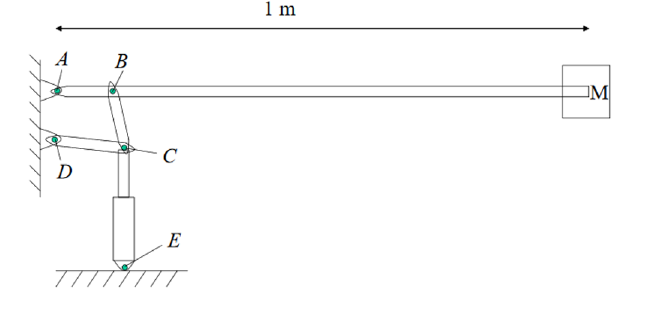
\includegraphics[width=\textwidth]{1_hydraulic_sim/BoomStructure.PNG}
    \caption{Hydraulic Boom Lift Structure}
    \label{fig:boom_structure}
\end{figure}


The square wave profile control signal shown in Figure \ref{fig:hydraulic_cs} is used as input to the simulation of the hydraulic system.
It stays at a neutral voltage of 0 until 0.2 seconds into the simulation.
At 0.2 seconds, the control signal is at its maximum of 10 volts for 0.4 seconds.
Then it falls to become proportionally negative at 0.7 seconds.
After another 0.4 seconds elapsed, the signal returns to the neural position of 0 volts beginning at 1.1 seconds.

\begin{figure}[H]
        %\centering
    %% Creator: Matplotlib, PGF backend
%%
%% To include the figure in your LaTeX document, write
%%   \input{<filename>.pgf}
%%
%% Make sure the required packages are loaded in your preamble
%%   \usepackage{pgf}
%%
%% Also ensure that all the required font packages are loaded; for instance,
%% the lmodern package is sometimes necessary when using math font.
%%   \usepackage{lmodern}
%%
%% Figures using additional raster images can only be included by \input if
%% they are in the same directory as the main LaTeX file. For loading figures
%% from other directories you can use the `import` package
%%   \usepackage{import}
%%
%% and then include the figures with
%%   \import{<path to file>}{<filename>.pgf}
%%
%% Matplotlib used the following preamble
%%
\begingroup%
\makeatletter%
\begin{pgfpicture}%
\pgfpathrectangle{\pgfpointorigin}{\pgfqpoint{6.000000in}{4.000000in}}%
\pgfusepath{use as bounding box, clip}%
\begin{pgfscope}%
\pgfsetbuttcap%
\pgfsetmiterjoin%
\pgfsetlinewidth{0.000000pt}%
\definecolor{currentstroke}{rgb}{1.000000,1.000000,1.000000}%
\pgfsetstrokecolor{currentstroke}%
\pgfsetstrokeopacity{0.000000}%
\pgfsetdash{}{0pt}%
\pgfpathmoveto{\pgfqpoint{0.000000in}{0.000000in}}%
\pgfpathlineto{\pgfqpoint{6.000000in}{0.000000in}}%
\pgfpathlineto{\pgfqpoint{6.000000in}{4.000000in}}%
\pgfpathlineto{\pgfqpoint{0.000000in}{4.000000in}}%
\pgfpathlineto{\pgfqpoint{0.000000in}{0.000000in}}%
\pgfpathclose%
\pgfusepath{}%
\end{pgfscope}%
\begin{pgfscope}%
\pgfsetbuttcap%
\pgfsetmiterjoin%
\definecolor{currentfill}{rgb}{1.000000,1.000000,1.000000}%
\pgfsetfillcolor{currentfill}%
\pgfsetlinewidth{0.000000pt}%
\definecolor{currentstroke}{rgb}{0.000000,0.000000,0.000000}%
\pgfsetstrokecolor{currentstroke}%
\pgfsetstrokeopacity{0.000000}%
\pgfsetdash{}{0pt}%
\pgfpathmoveto{\pgfqpoint{0.750000in}{0.500000in}}%
\pgfpathlineto{\pgfqpoint{5.400000in}{0.500000in}}%
\pgfpathlineto{\pgfqpoint{5.400000in}{3.520000in}}%
\pgfpathlineto{\pgfqpoint{0.750000in}{3.520000in}}%
\pgfpathlineto{\pgfqpoint{0.750000in}{0.500000in}}%
\pgfpathclose%
\pgfusepath{fill}%
\end{pgfscope}%
\begin{pgfscope}%
\pgfsetbuttcap%
\pgfsetroundjoin%
\definecolor{currentfill}{rgb}{0.000000,0.000000,0.000000}%
\pgfsetfillcolor{currentfill}%
\pgfsetlinewidth{0.803000pt}%
\definecolor{currentstroke}{rgb}{0.000000,0.000000,0.000000}%
\pgfsetstrokecolor{currentstroke}%
\pgfsetdash{}{0pt}%
\pgfsys@defobject{currentmarker}{\pgfqpoint{0.000000in}{-0.048611in}}{\pgfqpoint{0.000000in}{0.000000in}}{%
\pgfpathmoveto{\pgfqpoint{0.000000in}{0.000000in}}%
\pgfpathlineto{\pgfqpoint{0.000000in}{-0.048611in}}%
\pgfusepath{stroke,fill}%
}%
\begin{pgfscope}%
\pgfsys@transformshift{0.961364in}{0.500000in}%
\pgfsys@useobject{currentmarker}{}%
\end{pgfscope}%
\end{pgfscope}%
\begin{pgfscope}%
\definecolor{textcolor}{rgb}{0.000000,0.000000,0.000000}%
\pgfsetstrokecolor{textcolor}%
\pgfsetfillcolor{textcolor}%
\pgftext[x=0.961364in,y=0.402778in,,top]{\color{textcolor}\rmfamily\fontsize{10.000000}{12.000000}\selectfont \(\displaystyle {0.0}\)}%
\end{pgfscope}%
\begin{pgfscope}%
\pgfsetbuttcap%
\pgfsetroundjoin%
\definecolor{currentfill}{rgb}{0.000000,0.000000,0.000000}%
\pgfsetfillcolor{currentfill}%
\pgfsetlinewidth{0.803000pt}%
\definecolor{currentstroke}{rgb}{0.000000,0.000000,0.000000}%
\pgfsetstrokecolor{currentstroke}%
\pgfsetdash{}{0pt}%
\pgfsys@defobject{currentmarker}{\pgfqpoint{0.000000in}{-0.048611in}}{\pgfqpoint{0.000000in}{0.000000in}}{%
\pgfpathmoveto{\pgfqpoint{0.000000in}{0.000000in}}%
\pgfpathlineto{\pgfqpoint{0.000000in}{-0.048611in}}%
\pgfusepath{stroke,fill}%
}%
\begin{pgfscope}%
\pgfsys@transformshift{1.525000in}{0.500000in}%
\pgfsys@useobject{currentmarker}{}%
\end{pgfscope}%
\end{pgfscope}%
\begin{pgfscope}%
\definecolor{textcolor}{rgb}{0.000000,0.000000,0.000000}%
\pgfsetstrokecolor{textcolor}%
\pgfsetfillcolor{textcolor}%
\pgftext[x=1.525000in,y=0.402778in,,top]{\color{textcolor}\rmfamily\fontsize{10.000000}{12.000000}\selectfont \(\displaystyle {0.2}\)}%
\end{pgfscope}%
\begin{pgfscope}%
\pgfsetbuttcap%
\pgfsetroundjoin%
\definecolor{currentfill}{rgb}{0.000000,0.000000,0.000000}%
\pgfsetfillcolor{currentfill}%
\pgfsetlinewidth{0.803000pt}%
\definecolor{currentstroke}{rgb}{0.000000,0.000000,0.000000}%
\pgfsetstrokecolor{currentstroke}%
\pgfsetdash{}{0pt}%
\pgfsys@defobject{currentmarker}{\pgfqpoint{0.000000in}{-0.048611in}}{\pgfqpoint{0.000000in}{0.000000in}}{%
\pgfpathmoveto{\pgfqpoint{0.000000in}{0.000000in}}%
\pgfpathlineto{\pgfqpoint{0.000000in}{-0.048611in}}%
\pgfusepath{stroke,fill}%
}%
\begin{pgfscope}%
\pgfsys@transformshift{2.088636in}{0.500000in}%
\pgfsys@useobject{currentmarker}{}%
\end{pgfscope}%
\end{pgfscope}%
\begin{pgfscope}%
\definecolor{textcolor}{rgb}{0.000000,0.000000,0.000000}%
\pgfsetstrokecolor{textcolor}%
\pgfsetfillcolor{textcolor}%
\pgftext[x=2.088636in,y=0.402778in,,top]{\color{textcolor}\rmfamily\fontsize{10.000000}{12.000000}\selectfont \(\displaystyle {0.4}\)}%
\end{pgfscope}%
\begin{pgfscope}%
\pgfsetbuttcap%
\pgfsetroundjoin%
\definecolor{currentfill}{rgb}{0.000000,0.000000,0.000000}%
\pgfsetfillcolor{currentfill}%
\pgfsetlinewidth{0.803000pt}%
\definecolor{currentstroke}{rgb}{0.000000,0.000000,0.000000}%
\pgfsetstrokecolor{currentstroke}%
\pgfsetdash{}{0pt}%
\pgfsys@defobject{currentmarker}{\pgfqpoint{0.000000in}{-0.048611in}}{\pgfqpoint{0.000000in}{0.000000in}}{%
\pgfpathmoveto{\pgfqpoint{0.000000in}{0.000000in}}%
\pgfpathlineto{\pgfqpoint{0.000000in}{-0.048611in}}%
\pgfusepath{stroke,fill}%
}%
\begin{pgfscope}%
\pgfsys@transformshift{2.652273in}{0.500000in}%
\pgfsys@useobject{currentmarker}{}%
\end{pgfscope}%
\end{pgfscope}%
\begin{pgfscope}%
\definecolor{textcolor}{rgb}{0.000000,0.000000,0.000000}%
\pgfsetstrokecolor{textcolor}%
\pgfsetfillcolor{textcolor}%
\pgftext[x=2.652273in,y=0.402778in,,top]{\color{textcolor}\rmfamily\fontsize{10.000000}{12.000000}\selectfont \(\displaystyle {0.6}\)}%
\end{pgfscope}%
\begin{pgfscope}%
\pgfsetbuttcap%
\pgfsetroundjoin%
\definecolor{currentfill}{rgb}{0.000000,0.000000,0.000000}%
\pgfsetfillcolor{currentfill}%
\pgfsetlinewidth{0.803000pt}%
\definecolor{currentstroke}{rgb}{0.000000,0.000000,0.000000}%
\pgfsetstrokecolor{currentstroke}%
\pgfsetdash{}{0pt}%
\pgfsys@defobject{currentmarker}{\pgfqpoint{0.000000in}{-0.048611in}}{\pgfqpoint{0.000000in}{0.000000in}}{%
\pgfpathmoveto{\pgfqpoint{0.000000in}{0.000000in}}%
\pgfpathlineto{\pgfqpoint{0.000000in}{-0.048611in}}%
\pgfusepath{stroke,fill}%
}%
\begin{pgfscope}%
\pgfsys@transformshift{3.215909in}{0.500000in}%
\pgfsys@useobject{currentmarker}{}%
\end{pgfscope}%
\end{pgfscope}%
\begin{pgfscope}%
\definecolor{textcolor}{rgb}{0.000000,0.000000,0.000000}%
\pgfsetstrokecolor{textcolor}%
\pgfsetfillcolor{textcolor}%
\pgftext[x=3.215909in,y=0.402778in,,top]{\color{textcolor}\rmfamily\fontsize{10.000000}{12.000000}\selectfont \(\displaystyle {0.8}\)}%
\end{pgfscope}%
\begin{pgfscope}%
\pgfsetbuttcap%
\pgfsetroundjoin%
\definecolor{currentfill}{rgb}{0.000000,0.000000,0.000000}%
\pgfsetfillcolor{currentfill}%
\pgfsetlinewidth{0.803000pt}%
\definecolor{currentstroke}{rgb}{0.000000,0.000000,0.000000}%
\pgfsetstrokecolor{currentstroke}%
\pgfsetdash{}{0pt}%
\pgfsys@defobject{currentmarker}{\pgfqpoint{0.000000in}{-0.048611in}}{\pgfqpoint{0.000000in}{0.000000in}}{%
\pgfpathmoveto{\pgfqpoint{0.000000in}{0.000000in}}%
\pgfpathlineto{\pgfqpoint{0.000000in}{-0.048611in}}%
\pgfusepath{stroke,fill}%
}%
\begin{pgfscope}%
\pgfsys@transformshift{3.779545in}{0.500000in}%
\pgfsys@useobject{currentmarker}{}%
\end{pgfscope}%
\end{pgfscope}%
\begin{pgfscope}%
\definecolor{textcolor}{rgb}{0.000000,0.000000,0.000000}%
\pgfsetstrokecolor{textcolor}%
\pgfsetfillcolor{textcolor}%
\pgftext[x=3.779545in,y=0.402778in,,top]{\color{textcolor}\rmfamily\fontsize{10.000000}{12.000000}\selectfont \(\displaystyle {1.0}\)}%
\end{pgfscope}%
\begin{pgfscope}%
\pgfsetbuttcap%
\pgfsetroundjoin%
\definecolor{currentfill}{rgb}{0.000000,0.000000,0.000000}%
\pgfsetfillcolor{currentfill}%
\pgfsetlinewidth{0.803000pt}%
\definecolor{currentstroke}{rgb}{0.000000,0.000000,0.000000}%
\pgfsetstrokecolor{currentstroke}%
\pgfsetdash{}{0pt}%
\pgfsys@defobject{currentmarker}{\pgfqpoint{0.000000in}{-0.048611in}}{\pgfqpoint{0.000000in}{0.000000in}}{%
\pgfpathmoveto{\pgfqpoint{0.000000in}{0.000000in}}%
\pgfpathlineto{\pgfqpoint{0.000000in}{-0.048611in}}%
\pgfusepath{stroke,fill}%
}%
\begin{pgfscope}%
\pgfsys@transformshift{4.343182in}{0.500000in}%
\pgfsys@useobject{currentmarker}{}%
\end{pgfscope}%
\end{pgfscope}%
\begin{pgfscope}%
\definecolor{textcolor}{rgb}{0.000000,0.000000,0.000000}%
\pgfsetstrokecolor{textcolor}%
\pgfsetfillcolor{textcolor}%
\pgftext[x=4.343182in,y=0.402778in,,top]{\color{textcolor}\rmfamily\fontsize{10.000000}{12.000000}\selectfont \(\displaystyle {1.2}\)}%
\end{pgfscope}%
\begin{pgfscope}%
\pgfsetbuttcap%
\pgfsetroundjoin%
\definecolor{currentfill}{rgb}{0.000000,0.000000,0.000000}%
\pgfsetfillcolor{currentfill}%
\pgfsetlinewidth{0.803000pt}%
\definecolor{currentstroke}{rgb}{0.000000,0.000000,0.000000}%
\pgfsetstrokecolor{currentstroke}%
\pgfsetdash{}{0pt}%
\pgfsys@defobject{currentmarker}{\pgfqpoint{0.000000in}{-0.048611in}}{\pgfqpoint{0.000000in}{0.000000in}}{%
\pgfpathmoveto{\pgfqpoint{0.000000in}{0.000000in}}%
\pgfpathlineto{\pgfqpoint{0.000000in}{-0.048611in}}%
\pgfusepath{stroke,fill}%
}%
\begin{pgfscope}%
\pgfsys@transformshift{4.906818in}{0.500000in}%
\pgfsys@useobject{currentmarker}{}%
\end{pgfscope}%
\end{pgfscope}%
\begin{pgfscope}%
\definecolor{textcolor}{rgb}{0.000000,0.000000,0.000000}%
\pgfsetstrokecolor{textcolor}%
\pgfsetfillcolor{textcolor}%
\pgftext[x=4.906818in,y=0.402778in,,top]{\color{textcolor}\rmfamily\fontsize{10.000000}{12.000000}\selectfont \(\displaystyle {1.4}\)}%
\end{pgfscope}%
\begin{pgfscope}%
\definecolor{textcolor}{rgb}{0.000000,0.000000,0.000000}%
\pgfsetstrokecolor{textcolor}%
\pgfsetfillcolor{textcolor}%
\pgftext[x=3.075000in,y=0.223766in,,top]{\color{textcolor}\rmfamily\fontsize{10.000000}{12.000000}\selectfont Time (s)}%
\end{pgfscope}%
\begin{pgfscope}%
\pgfsetbuttcap%
\pgfsetroundjoin%
\definecolor{currentfill}{rgb}{0.000000,0.000000,0.000000}%
\pgfsetfillcolor{currentfill}%
\pgfsetlinewidth{0.803000pt}%
\definecolor{currentstroke}{rgb}{0.000000,0.000000,0.000000}%
\pgfsetstrokecolor{currentstroke}%
\pgfsetdash{}{0pt}%
\pgfsys@defobject{currentmarker}{\pgfqpoint{-0.048611in}{0.000000in}}{\pgfqpoint{-0.000000in}{0.000000in}}{%
\pgfpathmoveto{\pgfqpoint{-0.000000in}{0.000000in}}%
\pgfpathlineto{\pgfqpoint{-0.048611in}{0.000000in}}%
\pgfusepath{stroke,fill}%
}%
\begin{pgfscope}%
\pgfsys@transformshift{0.750000in}{0.637273in}%
\pgfsys@useobject{currentmarker}{}%
\end{pgfscope}%
\end{pgfscope}%
\begin{pgfscope}%
\definecolor{textcolor}{rgb}{0.000000,0.000000,0.000000}%
\pgfsetstrokecolor{textcolor}%
\pgfsetfillcolor{textcolor}%
\pgftext[x=0.297838in, y=0.589047in, left, base]{\color{textcolor}\rmfamily\fontsize{10.000000}{12.000000}\selectfont \(\displaystyle {\ensuremath{-}10.0}\)}%
\end{pgfscope}%
\begin{pgfscope}%
\pgfsetbuttcap%
\pgfsetroundjoin%
\definecolor{currentfill}{rgb}{0.000000,0.000000,0.000000}%
\pgfsetfillcolor{currentfill}%
\pgfsetlinewidth{0.803000pt}%
\definecolor{currentstroke}{rgb}{0.000000,0.000000,0.000000}%
\pgfsetstrokecolor{currentstroke}%
\pgfsetdash{}{0pt}%
\pgfsys@defobject{currentmarker}{\pgfqpoint{-0.048611in}{0.000000in}}{\pgfqpoint{-0.000000in}{0.000000in}}{%
\pgfpathmoveto{\pgfqpoint{-0.000000in}{0.000000in}}%
\pgfpathlineto{\pgfqpoint{-0.048611in}{0.000000in}}%
\pgfusepath{stroke,fill}%
}%
\begin{pgfscope}%
\pgfsys@transformshift{0.750000in}{0.980455in}%
\pgfsys@useobject{currentmarker}{}%
\end{pgfscope}%
\end{pgfscope}%
\begin{pgfscope}%
\definecolor{textcolor}{rgb}{0.000000,0.000000,0.000000}%
\pgfsetstrokecolor{textcolor}%
\pgfsetfillcolor{textcolor}%
\pgftext[x=0.367283in, y=0.932229in, left, base]{\color{textcolor}\rmfamily\fontsize{10.000000}{12.000000}\selectfont \(\displaystyle {\ensuremath{-}7.5}\)}%
\end{pgfscope}%
\begin{pgfscope}%
\pgfsetbuttcap%
\pgfsetroundjoin%
\definecolor{currentfill}{rgb}{0.000000,0.000000,0.000000}%
\pgfsetfillcolor{currentfill}%
\pgfsetlinewidth{0.803000pt}%
\definecolor{currentstroke}{rgb}{0.000000,0.000000,0.000000}%
\pgfsetstrokecolor{currentstroke}%
\pgfsetdash{}{0pt}%
\pgfsys@defobject{currentmarker}{\pgfqpoint{-0.048611in}{0.000000in}}{\pgfqpoint{-0.000000in}{0.000000in}}{%
\pgfpathmoveto{\pgfqpoint{-0.000000in}{0.000000in}}%
\pgfpathlineto{\pgfqpoint{-0.048611in}{0.000000in}}%
\pgfusepath{stroke,fill}%
}%
\begin{pgfscope}%
\pgfsys@transformshift{0.750000in}{1.323636in}%
\pgfsys@useobject{currentmarker}{}%
\end{pgfscope}%
\end{pgfscope}%
\begin{pgfscope}%
\definecolor{textcolor}{rgb}{0.000000,0.000000,0.000000}%
\pgfsetstrokecolor{textcolor}%
\pgfsetfillcolor{textcolor}%
\pgftext[x=0.367283in, y=1.275411in, left, base]{\color{textcolor}\rmfamily\fontsize{10.000000}{12.000000}\selectfont \(\displaystyle {\ensuremath{-}5.0}\)}%
\end{pgfscope}%
\begin{pgfscope}%
\pgfsetbuttcap%
\pgfsetroundjoin%
\definecolor{currentfill}{rgb}{0.000000,0.000000,0.000000}%
\pgfsetfillcolor{currentfill}%
\pgfsetlinewidth{0.803000pt}%
\definecolor{currentstroke}{rgb}{0.000000,0.000000,0.000000}%
\pgfsetstrokecolor{currentstroke}%
\pgfsetdash{}{0pt}%
\pgfsys@defobject{currentmarker}{\pgfqpoint{-0.048611in}{0.000000in}}{\pgfqpoint{-0.000000in}{0.000000in}}{%
\pgfpathmoveto{\pgfqpoint{-0.000000in}{0.000000in}}%
\pgfpathlineto{\pgfqpoint{-0.048611in}{0.000000in}}%
\pgfusepath{stroke,fill}%
}%
\begin{pgfscope}%
\pgfsys@transformshift{0.750000in}{1.666818in}%
\pgfsys@useobject{currentmarker}{}%
\end{pgfscope}%
\end{pgfscope}%
\begin{pgfscope}%
\definecolor{textcolor}{rgb}{0.000000,0.000000,0.000000}%
\pgfsetstrokecolor{textcolor}%
\pgfsetfillcolor{textcolor}%
\pgftext[x=0.367283in, y=1.618593in, left, base]{\color{textcolor}\rmfamily\fontsize{10.000000}{12.000000}\selectfont \(\displaystyle {\ensuremath{-}2.5}\)}%
\end{pgfscope}%
\begin{pgfscope}%
\pgfsetbuttcap%
\pgfsetroundjoin%
\definecolor{currentfill}{rgb}{0.000000,0.000000,0.000000}%
\pgfsetfillcolor{currentfill}%
\pgfsetlinewidth{0.803000pt}%
\definecolor{currentstroke}{rgb}{0.000000,0.000000,0.000000}%
\pgfsetstrokecolor{currentstroke}%
\pgfsetdash{}{0pt}%
\pgfsys@defobject{currentmarker}{\pgfqpoint{-0.048611in}{0.000000in}}{\pgfqpoint{-0.000000in}{0.000000in}}{%
\pgfpathmoveto{\pgfqpoint{-0.000000in}{0.000000in}}%
\pgfpathlineto{\pgfqpoint{-0.048611in}{0.000000in}}%
\pgfusepath{stroke,fill}%
}%
\begin{pgfscope}%
\pgfsys@transformshift{0.750000in}{2.010000in}%
\pgfsys@useobject{currentmarker}{}%
\end{pgfscope}%
\end{pgfscope}%
\begin{pgfscope}%
\definecolor{textcolor}{rgb}{0.000000,0.000000,0.000000}%
\pgfsetstrokecolor{textcolor}%
\pgfsetfillcolor{textcolor}%
\pgftext[x=0.475308in, y=1.961775in, left, base]{\color{textcolor}\rmfamily\fontsize{10.000000}{12.000000}\selectfont \(\displaystyle {0.0}\)}%
\end{pgfscope}%
\begin{pgfscope}%
\pgfsetbuttcap%
\pgfsetroundjoin%
\definecolor{currentfill}{rgb}{0.000000,0.000000,0.000000}%
\pgfsetfillcolor{currentfill}%
\pgfsetlinewidth{0.803000pt}%
\definecolor{currentstroke}{rgb}{0.000000,0.000000,0.000000}%
\pgfsetstrokecolor{currentstroke}%
\pgfsetdash{}{0pt}%
\pgfsys@defobject{currentmarker}{\pgfqpoint{-0.048611in}{0.000000in}}{\pgfqpoint{-0.000000in}{0.000000in}}{%
\pgfpathmoveto{\pgfqpoint{-0.000000in}{0.000000in}}%
\pgfpathlineto{\pgfqpoint{-0.048611in}{0.000000in}}%
\pgfusepath{stroke,fill}%
}%
\begin{pgfscope}%
\pgfsys@transformshift{0.750000in}{2.353182in}%
\pgfsys@useobject{currentmarker}{}%
\end{pgfscope}%
\end{pgfscope}%
\begin{pgfscope}%
\definecolor{textcolor}{rgb}{0.000000,0.000000,0.000000}%
\pgfsetstrokecolor{textcolor}%
\pgfsetfillcolor{textcolor}%
\pgftext[x=0.475308in, y=2.304957in, left, base]{\color{textcolor}\rmfamily\fontsize{10.000000}{12.000000}\selectfont \(\displaystyle {2.5}\)}%
\end{pgfscope}%
\begin{pgfscope}%
\pgfsetbuttcap%
\pgfsetroundjoin%
\definecolor{currentfill}{rgb}{0.000000,0.000000,0.000000}%
\pgfsetfillcolor{currentfill}%
\pgfsetlinewidth{0.803000pt}%
\definecolor{currentstroke}{rgb}{0.000000,0.000000,0.000000}%
\pgfsetstrokecolor{currentstroke}%
\pgfsetdash{}{0pt}%
\pgfsys@defobject{currentmarker}{\pgfqpoint{-0.048611in}{0.000000in}}{\pgfqpoint{-0.000000in}{0.000000in}}{%
\pgfpathmoveto{\pgfqpoint{-0.000000in}{0.000000in}}%
\pgfpathlineto{\pgfqpoint{-0.048611in}{0.000000in}}%
\pgfusepath{stroke,fill}%
}%
\begin{pgfscope}%
\pgfsys@transformshift{0.750000in}{2.696364in}%
\pgfsys@useobject{currentmarker}{}%
\end{pgfscope}%
\end{pgfscope}%
\begin{pgfscope}%
\definecolor{textcolor}{rgb}{0.000000,0.000000,0.000000}%
\pgfsetstrokecolor{textcolor}%
\pgfsetfillcolor{textcolor}%
\pgftext[x=0.475308in, y=2.648138in, left, base]{\color{textcolor}\rmfamily\fontsize{10.000000}{12.000000}\selectfont \(\displaystyle {5.0}\)}%
\end{pgfscope}%
\begin{pgfscope}%
\pgfsetbuttcap%
\pgfsetroundjoin%
\definecolor{currentfill}{rgb}{0.000000,0.000000,0.000000}%
\pgfsetfillcolor{currentfill}%
\pgfsetlinewidth{0.803000pt}%
\definecolor{currentstroke}{rgb}{0.000000,0.000000,0.000000}%
\pgfsetstrokecolor{currentstroke}%
\pgfsetdash{}{0pt}%
\pgfsys@defobject{currentmarker}{\pgfqpoint{-0.048611in}{0.000000in}}{\pgfqpoint{-0.000000in}{0.000000in}}{%
\pgfpathmoveto{\pgfqpoint{-0.000000in}{0.000000in}}%
\pgfpathlineto{\pgfqpoint{-0.048611in}{0.000000in}}%
\pgfusepath{stroke,fill}%
}%
\begin{pgfscope}%
\pgfsys@transformshift{0.750000in}{3.039545in}%
\pgfsys@useobject{currentmarker}{}%
\end{pgfscope}%
\end{pgfscope}%
\begin{pgfscope}%
\definecolor{textcolor}{rgb}{0.000000,0.000000,0.000000}%
\pgfsetstrokecolor{textcolor}%
\pgfsetfillcolor{textcolor}%
\pgftext[x=0.475308in, y=2.991320in, left, base]{\color{textcolor}\rmfamily\fontsize{10.000000}{12.000000}\selectfont \(\displaystyle {7.5}\)}%
\end{pgfscope}%
\begin{pgfscope}%
\pgfsetbuttcap%
\pgfsetroundjoin%
\definecolor{currentfill}{rgb}{0.000000,0.000000,0.000000}%
\pgfsetfillcolor{currentfill}%
\pgfsetlinewidth{0.803000pt}%
\definecolor{currentstroke}{rgb}{0.000000,0.000000,0.000000}%
\pgfsetstrokecolor{currentstroke}%
\pgfsetdash{}{0pt}%
\pgfsys@defobject{currentmarker}{\pgfqpoint{-0.048611in}{0.000000in}}{\pgfqpoint{-0.000000in}{0.000000in}}{%
\pgfpathmoveto{\pgfqpoint{-0.000000in}{0.000000in}}%
\pgfpathlineto{\pgfqpoint{-0.048611in}{0.000000in}}%
\pgfusepath{stroke,fill}%
}%
\begin{pgfscope}%
\pgfsys@transformshift{0.750000in}{3.382727in}%
\pgfsys@useobject{currentmarker}{}%
\end{pgfscope}%
\end{pgfscope}%
\begin{pgfscope}%
\definecolor{textcolor}{rgb}{0.000000,0.000000,0.000000}%
\pgfsetstrokecolor{textcolor}%
\pgfsetfillcolor{textcolor}%
\pgftext[x=0.405863in, y=3.334502in, left, base]{\color{textcolor}\rmfamily\fontsize{10.000000}{12.000000}\selectfont \(\displaystyle {10.0}\)}%
\end{pgfscope}%
\begin{pgfscope}%
\definecolor{textcolor}{rgb}{0.000000,0.000000,0.000000}%
\pgfsetstrokecolor{textcolor}%
\pgfsetfillcolor{textcolor}%
\pgftext[x=0.242283in,y=2.010000in,,bottom,rotate=90.000000]{\color{textcolor}\rmfamily\fontsize{10.000000}{12.000000}\selectfont Voltage (\(\displaystyle V\))}%
\end{pgfscope}%
\begin{pgfscope}%
\pgfpathrectangle{\pgfqpoint{0.750000in}{0.500000in}}{\pgfqpoint{4.650000in}{3.020000in}}%
\pgfusepath{clip}%
\pgfsetrectcap%
\pgfsetroundjoin%
\pgfsetlinewidth{1.505625pt}%
\definecolor{currentstroke}{rgb}{0.121569,0.466667,0.705882}%
\pgfsetstrokecolor{currentstroke}%
\pgfsetdash{}{0pt}%
\pgfpathmoveto{\pgfqpoint{0.961364in}{2.010000in}}%
\pgfpathlineto{\pgfqpoint{1.525156in}{2.011521in}}%
\pgfpathlineto{\pgfqpoint{1.665909in}{3.382727in}}%
\pgfpathlineto{\pgfqpoint{1.665909in}{3.382727in}}%
\pgfpathlineto{\pgfqpoint{2.652273in}{3.382727in}}%
\pgfpathlineto{\pgfqpoint{2.652273in}{3.382727in}}%
\pgfpathlineto{\pgfqpoint{2.934091in}{0.637273in}}%
\pgfpathlineto{\pgfqpoint{2.934091in}{0.637273in}}%
\pgfpathlineto{\pgfqpoint{3.920455in}{0.637273in}}%
\pgfpathlineto{\pgfqpoint{3.920455in}{0.637273in}}%
\pgfpathlineto{\pgfqpoint{4.062434in}{2.010001in}}%
\pgfpathlineto{\pgfqpoint{4.062434in}{2.010001in}}%
\pgfpathlineto{\pgfqpoint{5.188636in}{2.011445in}}%
\pgfpathlineto{\pgfqpoint{5.188636in}{2.011445in}}%
\pgfusepath{stroke}%
\end{pgfscope}%
\begin{pgfscope}%
\pgfsetrectcap%
\pgfsetmiterjoin%
\pgfsetlinewidth{0.803000pt}%
\definecolor{currentstroke}{rgb}{0.000000,0.000000,0.000000}%
\pgfsetstrokecolor{currentstroke}%
\pgfsetdash{}{0pt}%
\pgfpathmoveto{\pgfqpoint{0.750000in}{0.500000in}}%
\pgfpathlineto{\pgfqpoint{0.750000in}{3.520000in}}%
\pgfusepath{stroke}%
\end{pgfscope}%
\begin{pgfscope}%
\pgfsetrectcap%
\pgfsetmiterjoin%
\pgfsetlinewidth{0.803000pt}%
\definecolor{currentstroke}{rgb}{0.000000,0.000000,0.000000}%
\pgfsetstrokecolor{currentstroke}%
\pgfsetdash{}{0pt}%
\pgfpathmoveto{\pgfqpoint{5.400000in}{0.500000in}}%
\pgfpathlineto{\pgfqpoint{5.400000in}{3.520000in}}%
\pgfusepath{stroke}%
\end{pgfscope}%
\begin{pgfscope}%
\pgfsetrectcap%
\pgfsetmiterjoin%
\pgfsetlinewidth{0.803000pt}%
\definecolor{currentstroke}{rgb}{0.000000,0.000000,0.000000}%
\pgfsetstrokecolor{currentstroke}%
\pgfsetdash{}{0pt}%
\pgfpathmoveto{\pgfqpoint{0.750000in}{0.500000in}}%
\pgfpathlineto{\pgfqpoint{5.400000in}{0.500000in}}%
\pgfusepath{stroke}%
\end{pgfscope}%
\begin{pgfscope}%
\pgfsetrectcap%
\pgfsetmiterjoin%
\pgfsetlinewidth{0.803000pt}%
\definecolor{currentstroke}{rgb}{0.000000,0.000000,0.000000}%
\pgfsetstrokecolor{currentstroke}%
\pgfsetdash{}{0pt}%
\pgfpathmoveto{\pgfqpoint{0.750000in}{3.520000in}}%
\pgfpathlineto{\pgfqpoint{5.400000in}{3.520000in}}%
\pgfusepath{stroke}%
\end{pgfscope}%
\end{pgfpicture}%
\makeatother%
\endgroup%

    \caption{Hydraulic System Control Signal}
    \label{fig:hydraulic_cs}
\end{figure}

Figure \ref{fig:hydraulic_pos} shows that introducing a proportionally negative signal does not cause the end effector to return to its initial position.
As the control signal is varied inversely, the position of the end effector only returns halfway to its initial position.
This indicates the system exhibits a non-linear relationship between the control signal and the end effector position.
The system experiences mild oscillation after coming to rest when the control signal returns to zero at the end of the simulation.
To achieve predictable system response and reduce oscillation, a more complex control methodology is required.

\begin{figure}[H]
        %\centering
    %% Creator: Matplotlib, PGF backend
%%
%% To include the figure in your LaTeX document, write
%%   \input{<filename>.pgf}
%%
%% Make sure the required packages are loaded in your preamble
%%   \usepackage{pgf}
%%
%% Also ensure that all the required font packages are loaded; for instance,
%% the lmodern package is sometimes necessary when using math font.
%%   \usepackage{lmodern}
%%
%% Figures using additional raster images can only be included by \input if
%% they are in the same directory as the main LaTeX file. For loading figures
%% from other directories you can use the `import` package
%%   \usepackage{import}
%%
%% and then include the figures with
%%   \import{<path to file>}{<filename>.pgf}
%%
%% Matplotlib used the following preamble
%%   \usepackage{fontspec}
%%   \setmainfont{DejaVuSerif.ttf}[Path=\detokenize{/Users/abeattie/miniconda/envs/masters-thesis/lib/python3.10/site-packages/matplotlib/mpl-data/fonts/ttf/}]
%%   \setsansfont{DejaVuSans.ttf}[Path=\detokenize{/Users/abeattie/miniconda/envs/masters-thesis/lib/python3.10/site-packages/matplotlib/mpl-data/fonts/ttf/}]
%%   \setmonofont{DejaVuSansMono.ttf}[Path=\detokenize{/Users/abeattie/miniconda/envs/masters-thesis/lib/python3.10/site-packages/matplotlib/mpl-data/fonts/ttf/}]
%%
\begingroup%
\makeatletter%
\begin{pgfpicture}%
\pgfpathrectangle{\pgfpointorigin}{\pgfqpoint{6.000000in}{4.000000in}}%
\pgfusepath{use as bounding box, clip}%
\begin{pgfscope}%
\pgfsetbuttcap%
\pgfsetmiterjoin%
\pgfsetlinewidth{0.000000pt}%
\definecolor{currentstroke}{rgb}{1.000000,1.000000,1.000000}%
\pgfsetstrokecolor{currentstroke}%
\pgfsetstrokeopacity{0.000000}%
\pgfsetdash{}{0pt}%
\pgfpathmoveto{\pgfqpoint{0.000000in}{0.000000in}}%
\pgfpathlineto{\pgfqpoint{6.000000in}{0.000000in}}%
\pgfpathlineto{\pgfqpoint{6.000000in}{4.000000in}}%
\pgfpathlineto{\pgfqpoint{0.000000in}{4.000000in}}%
\pgfpathlineto{\pgfqpoint{0.000000in}{0.000000in}}%
\pgfpathclose%
\pgfusepath{}%
\end{pgfscope}%
\end{pgfpicture}%
\makeatother%
\endgroup%

    \caption{Hydraulic Crane End Effector Position}
    \label{fig:hydraulic_pos}
\end{figure}

\subsubsection{Power Electronic Converter Dataset}
\label{ref_pec_dataset}

Transitioning from conventional power systems to power electronics-dominated grids (PEDG) has increased demand for grid-forming converters (GFM) to facilitate operational reliability.
GFMs have made significant progress in recent years to expedite stability under different grid conditions, but their operation during faults or large signal disturbances still remains a challenge.

Authors \cite{trainsient-stability-9523750} explain that GFMs handle a significantly smaller percentage of over-current (usually only 20\%) compared to synchronous generators (SGs) which can handle seven times their nominal current.
This makes fault detection for GFMs critical to maintain synchronization with the grid.
Since the network infrastructure of power systems keeps expanding, it is important to identify these faults accurately under varying grid parameter uncertainties.

This study examines four faults in the PEC dataset.
The frequency [$f_c$] of the system throughout various fault conditions is used for detection.
Each fault has significantly different characteristics and magnitude.
The faults examined in the study are explained in Table \ref{tab:pec_faults_table}.

\bigskip
\begin{longtable}{P{2cm} P{3.5cm} l}
\caption{PEC Dataset Classifications} \\
\toprule
\textbf{Fault} & \textbf{Description} & \textbf{Frequency Shape} \\
\midrule
\endfirsthead
\multicolumn{3}{c}%
{\tablename\ \thetable\ -- \textit{Continued from previous page}} \\
\hline
\textbf{Fault} & \textbf{Description} & \textbf{Frequency Shape} \\
\hline
\endhead
\hline \multicolumn{3}{r}{\textit{Continued on next page}} \\
\endfoot
\hline
\endlastfoot
    Line-to-Line (LL) Fault & This fault occurs when there is a short circuit between two conductors. & 
    \raisebox{-0.9\totalheight}{\resizebox{8cm}{!}{%% Creator: Matplotlib, PGF backend
%%
%% To include the figure in your LaTeX document, write
%%   \input{<filename>.pgf}
%%
%% Make sure the required packages are loaded in your preamble
%%   \usepackage{pgf}
%%
%% Also ensure that all the required font packages are loaded; for instance,
%% the lmodern package is sometimes necessary when using math font.
%%   \usepackage{lmodern}
%%
%% Figures using additional raster images can only be included by \input if
%% they are in the same directory as the main LaTeX file. For loading figures
%% from other directories you can use the `import` package
%%   \usepackage{import}
%%
%% and then include the figures with
%%   \import{<path to file>}{<filename>.pgf}
%%
%% Matplotlib used the following preamble
%%
\begingroup%
\makeatletter%
\begin{pgfpicture}%
\pgfpathrectangle{\pgfpointorigin}{\pgfqpoint{5.000000in}{4.000000in}}%
\pgfusepath{use as bounding box, clip}%
\begin{pgfscope}%
\pgfsetbuttcap%
\pgfsetmiterjoin%
\pgfsetlinewidth{0.000000pt}%
\definecolor{currentstroke}{rgb}{1.000000,1.000000,1.000000}%
\pgfsetstrokecolor{currentstroke}%
\pgfsetstrokeopacity{0.000000}%
\pgfsetdash{}{0pt}%
\pgfpathmoveto{\pgfqpoint{0.000000in}{0.000000in}}%
\pgfpathlineto{\pgfqpoint{5.000000in}{0.000000in}}%
\pgfpathlineto{\pgfqpoint{5.000000in}{4.000000in}}%
\pgfpathlineto{\pgfqpoint{0.000000in}{4.000000in}}%
\pgfpathlineto{\pgfqpoint{0.000000in}{0.000000in}}%
\pgfpathclose%
\pgfusepath{}%
\end{pgfscope}%
\begin{pgfscope}%
\pgfsetbuttcap%
\pgfsetmiterjoin%
\definecolor{currentfill}{rgb}{1.000000,1.000000,1.000000}%
\pgfsetfillcolor{currentfill}%
\pgfsetlinewidth{0.000000pt}%
\definecolor{currentstroke}{rgb}{0.000000,0.000000,0.000000}%
\pgfsetstrokecolor{currentstroke}%
\pgfsetstrokeopacity{0.000000}%
\pgfsetdash{}{0pt}%
\pgfpathmoveto{\pgfqpoint{0.625000in}{0.500000in}}%
\pgfpathlineto{\pgfqpoint{4.500000in}{0.500000in}}%
\pgfpathlineto{\pgfqpoint{4.500000in}{3.520000in}}%
\pgfpathlineto{\pgfqpoint{0.625000in}{3.520000in}}%
\pgfpathlineto{\pgfqpoint{0.625000in}{0.500000in}}%
\pgfpathclose%
\pgfusepath{fill}%
\end{pgfscope}%
\begin{pgfscope}%
\pgfsetbuttcap%
\pgfsetroundjoin%
\definecolor{currentfill}{rgb}{0.000000,0.000000,0.000000}%
\pgfsetfillcolor{currentfill}%
\pgfsetlinewidth{0.803000pt}%
\definecolor{currentstroke}{rgb}{0.000000,0.000000,0.000000}%
\pgfsetstrokecolor{currentstroke}%
\pgfsetdash{}{0pt}%
\pgfsys@defobject{currentmarker}{\pgfqpoint{0.000000in}{-0.048611in}}{\pgfqpoint{0.000000in}{0.000000in}}{%
\pgfpathmoveto{\pgfqpoint{0.000000in}{0.000000in}}%
\pgfpathlineto{\pgfqpoint{0.000000in}{-0.048611in}}%
\pgfusepath{stroke,fill}%
}%
\begin{pgfscope}%
\pgfsys@transformshift{0.801136in}{0.500000in}%
\pgfsys@useobject{currentmarker}{}%
\end{pgfscope}%
\end{pgfscope}%
\begin{pgfscope}%
\definecolor{textcolor}{rgb}{0.000000,0.000000,0.000000}%
\pgfsetstrokecolor{textcolor}%
\pgfsetfillcolor{textcolor}%
\pgftext[x=0.801136in,y=0.402778in,,top]{\color{textcolor}\rmfamily\fontsize{10.000000}{12.000000}\selectfont \(\displaystyle {40200}\)}%
\end{pgfscope}%
\begin{pgfscope}%
\pgfsetbuttcap%
\pgfsetroundjoin%
\definecolor{currentfill}{rgb}{0.000000,0.000000,0.000000}%
\pgfsetfillcolor{currentfill}%
\pgfsetlinewidth{0.803000pt}%
\definecolor{currentstroke}{rgb}{0.000000,0.000000,0.000000}%
\pgfsetstrokecolor{currentstroke}%
\pgfsetdash{}{0pt}%
\pgfsys@defobject{currentmarker}{\pgfqpoint{0.000000in}{-0.048611in}}{\pgfqpoint{0.000000in}{0.000000in}}{%
\pgfpathmoveto{\pgfqpoint{0.000000in}{0.000000in}}%
\pgfpathlineto{\pgfqpoint{0.000000in}{-0.048611in}}%
\pgfusepath{stroke,fill}%
}%
\begin{pgfscope}%
\pgfsys@transformshift{1.506387in}{0.500000in}%
\pgfsys@useobject{currentmarker}{}%
\end{pgfscope}%
\end{pgfscope}%
\begin{pgfscope}%
\definecolor{textcolor}{rgb}{0.000000,0.000000,0.000000}%
\pgfsetstrokecolor{textcolor}%
\pgfsetfillcolor{textcolor}%
\pgftext[x=1.506387in,y=0.402778in,,top]{\color{textcolor}\rmfamily\fontsize{10.000000}{12.000000}\selectfont \(\displaystyle {40400}\)}%
\end{pgfscope}%
\begin{pgfscope}%
\pgfsetbuttcap%
\pgfsetroundjoin%
\definecolor{currentfill}{rgb}{0.000000,0.000000,0.000000}%
\pgfsetfillcolor{currentfill}%
\pgfsetlinewidth{0.803000pt}%
\definecolor{currentstroke}{rgb}{0.000000,0.000000,0.000000}%
\pgfsetstrokecolor{currentstroke}%
\pgfsetdash{}{0pt}%
\pgfsys@defobject{currentmarker}{\pgfqpoint{0.000000in}{-0.048611in}}{\pgfqpoint{0.000000in}{0.000000in}}{%
\pgfpathmoveto{\pgfqpoint{0.000000in}{0.000000in}}%
\pgfpathlineto{\pgfqpoint{0.000000in}{-0.048611in}}%
\pgfusepath{stroke,fill}%
}%
\begin{pgfscope}%
\pgfsys@transformshift{2.211638in}{0.500000in}%
\pgfsys@useobject{currentmarker}{}%
\end{pgfscope}%
\end{pgfscope}%
\begin{pgfscope}%
\definecolor{textcolor}{rgb}{0.000000,0.000000,0.000000}%
\pgfsetstrokecolor{textcolor}%
\pgfsetfillcolor{textcolor}%
\pgftext[x=2.211638in,y=0.402778in,,top]{\color{textcolor}\rmfamily\fontsize{10.000000}{12.000000}\selectfont \(\displaystyle {40600}\)}%
\end{pgfscope}%
\begin{pgfscope}%
\pgfsetbuttcap%
\pgfsetroundjoin%
\definecolor{currentfill}{rgb}{0.000000,0.000000,0.000000}%
\pgfsetfillcolor{currentfill}%
\pgfsetlinewidth{0.803000pt}%
\definecolor{currentstroke}{rgb}{0.000000,0.000000,0.000000}%
\pgfsetstrokecolor{currentstroke}%
\pgfsetdash{}{0pt}%
\pgfsys@defobject{currentmarker}{\pgfqpoint{0.000000in}{-0.048611in}}{\pgfqpoint{0.000000in}{0.000000in}}{%
\pgfpathmoveto{\pgfqpoint{0.000000in}{0.000000in}}%
\pgfpathlineto{\pgfqpoint{0.000000in}{-0.048611in}}%
\pgfusepath{stroke,fill}%
}%
\begin{pgfscope}%
\pgfsys@transformshift{2.916888in}{0.500000in}%
\pgfsys@useobject{currentmarker}{}%
\end{pgfscope}%
\end{pgfscope}%
\begin{pgfscope}%
\definecolor{textcolor}{rgb}{0.000000,0.000000,0.000000}%
\pgfsetstrokecolor{textcolor}%
\pgfsetfillcolor{textcolor}%
\pgftext[x=2.916888in,y=0.402778in,,top]{\color{textcolor}\rmfamily\fontsize{10.000000}{12.000000}\selectfont \(\displaystyle {40800}\)}%
\end{pgfscope}%
\begin{pgfscope}%
\pgfsetbuttcap%
\pgfsetroundjoin%
\definecolor{currentfill}{rgb}{0.000000,0.000000,0.000000}%
\pgfsetfillcolor{currentfill}%
\pgfsetlinewidth{0.803000pt}%
\definecolor{currentstroke}{rgb}{0.000000,0.000000,0.000000}%
\pgfsetstrokecolor{currentstroke}%
\pgfsetdash{}{0pt}%
\pgfsys@defobject{currentmarker}{\pgfqpoint{0.000000in}{-0.048611in}}{\pgfqpoint{0.000000in}{0.000000in}}{%
\pgfpathmoveto{\pgfqpoint{0.000000in}{0.000000in}}%
\pgfpathlineto{\pgfqpoint{0.000000in}{-0.048611in}}%
\pgfusepath{stroke,fill}%
}%
\begin{pgfscope}%
\pgfsys@transformshift{3.622139in}{0.500000in}%
\pgfsys@useobject{currentmarker}{}%
\end{pgfscope}%
\end{pgfscope}%
\begin{pgfscope}%
\definecolor{textcolor}{rgb}{0.000000,0.000000,0.000000}%
\pgfsetstrokecolor{textcolor}%
\pgfsetfillcolor{textcolor}%
\pgftext[x=3.622139in,y=0.402778in,,top]{\color{textcolor}\rmfamily\fontsize{10.000000}{12.000000}\selectfont \(\displaystyle {41000}\)}%
\end{pgfscope}%
\begin{pgfscope}%
\pgfsetbuttcap%
\pgfsetroundjoin%
\definecolor{currentfill}{rgb}{0.000000,0.000000,0.000000}%
\pgfsetfillcolor{currentfill}%
\pgfsetlinewidth{0.803000pt}%
\definecolor{currentstroke}{rgb}{0.000000,0.000000,0.000000}%
\pgfsetstrokecolor{currentstroke}%
\pgfsetdash{}{0pt}%
\pgfsys@defobject{currentmarker}{\pgfqpoint{0.000000in}{-0.048611in}}{\pgfqpoint{0.000000in}{0.000000in}}{%
\pgfpathmoveto{\pgfqpoint{0.000000in}{0.000000in}}%
\pgfpathlineto{\pgfqpoint{0.000000in}{-0.048611in}}%
\pgfusepath{stroke,fill}%
}%
\begin{pgfscope}%
\pgfsys@transformshift{4.327390in}{0.500000in}%
\pgfsys@useobject{currentmarker}{}%
\end{pgfscope}%
\end{pgfscope}%
\begin{pgfscope}%
\definecolor{textcolor}{rgb}{0.000000,0.000000,0.000000}%
\pgfsetstrokecolor{textcolor}%
\pgfsetfillcolor{textcolor}%
\pgftext[x=4.327390in,y=0.402778in,,top]{\color{textcolor}\rmfamily\fontsize{10.000000}{12.000000}\selectfont \(\displaystyle {41200}\)}%
\end{pgfscope}%
\begin{pgfscope}%
\definecolor{textcolor}{rgb}{0.000000,0.000000,0.000000}%
\pgfsetstrokecolor{textcolor}%
\pgfsetfillcolor{textcolor}%
\pgftext[x=2.562500in,y=0.223766in,,top]{\color{textcolor}\rmfamily\fontsize{10.000000}{12.000000}\selectfont Time (s)}%
\end{pgfscope}%
\begin{pgfscope}%
\pgfsetbuttcap%
\pgfsetroundjoin%
\definecolor{currentfill}{rgb}{0.000000,0.000000,0.000000}%
\pgfsetfillcolor{currentfill}%
\pgfsetlinewidth{0.803000pt}%
\definecolor{currentstroke}{rgb}{0.000000,0.000000,0.000000}%
\pgfsetstrokecolor{currentstroke}%
\pgfsetdash{}{0pt}%
\pgfsys@defobject{currentmarker}{\pgfqpoint{-0.048611in}{0.000000in}}{\pgfqpoint{-0.000000in}{0.000000in}}{%
\pgfpathmoveto{\pgfqpoint{-0.000000in}{0.000000in}}%
\pgfpathlineto{\pgfqpoint{-0.048611in}{0.000000in}}%
\pgfusepath{stroke,fill}%
}%
\begin{pgfscope}%
\pgfsys@transformshift{0.625000in}{0.686723in}%
\pgfsys@useobject{currentmarker}{}%
\end{pgfscope}%
\end{pgfscope}%
\begin{pgfscope}%
\definecolor{textcolor}{rgb}{0.000000,0.000000,0.000000}%
\pgfsetstrokecolor{textcolor}%
\pgfsetfillcolor{textcolor}%
\pgftext[x=0.350308in, y=0.638498in, left, base]{\color{textcolor}\rmfamily\fontsize{10.000000}{12.000000}\selectfont \(\displaystyle {\ensuremath{-}7}\)}%
\end{pgfscope}%
\begin{pgfscope}%
\pgfsetbuttcap%
\pgfsetroundjoin%
\definecolor{currentfill}{rgb}{0.000000,0.000000,0.000000}%
\pgfsetfillcolor{currentfill}%
\pgfsetlinewidth{0.803000pt}%
\definecolor{currentstroke}{rgb}{0.000000,0.000000,0.000000}%
\pgfsetstrokecolor{currentstroke}%
\pgfsetdash{}{0pt}%
\pgfsys@defobject{currentmarker}{\pgfqpoint{-0.048611in}{0.000000in}}{\pgfqpoint{-0.000000in}{0.000000in}}{%
\pgfpathmoveto{\pgfqpoint{-0.000000in}{0.000000in}}%
\pgfpathlineto{\pgfqpoint{-0.048611in}{0.000000in}}%
\pgfusepath{stroke,fill}%
}%
\begin{pgfscope}%
\pgfsys@transformshift{0.625000in}{1.069135in}%
\pgfsys@useobject{currentmarker}{}%
\end{pgfscope}%
\end{pgfscope}%
\begin{pgfscope}%
\definecolor{textcolor}{rgb}{0.000000,0.000000,0.000000}%
\pgfsetstrokecolor{textcolor}%
\pgfsetfillcolor{textcolor}%
\pgftext[x=0.350308in, y=1.020910in, left, base]{\color{textcolor}\rmfamily\fontsize{10.000000}{12.000000}\selectfont \(\displaystyle {\ensuremath{-}6}\)}%
\end{pgfscope}%
\begin{pgfscope}%
\pgfsetbuttcap%
\pgfsetroundjoin%
\definecolor{currentfill}{rgb}{0.000000,0.000000,0.000000}%
\pgfsetfillcolor{currentfill}%
\pgfsetlinewidth{0.803000pt}%
\definecolor{currentstroke}{rgb}{0.000000,0.000000,0.000000}%
\pgfsetstrokecolor{currentstroke}%
\pgfsetdash{}{0pt}%
\pgfsys@defobject{currentmarker}{\pgfqpoint{-0.048611in}{0.000000in}}{\pgfqpoint{-0.000000in}{0.000000in}}{%
\pgfpathmoveto{\pgfqpoint{-0.000000in}{0.000000in}}%
\pgfpathlineto{\pgfqpoint{-0.048611in}{0.000000in}}%
\pgfusepath{stroke,fill}%
}%
\begin{pgfscope}%
\pgfsys@transformshift{0.625000in}{1.451547in}%
\pgfsys@useobject{currentmarker}{}%
\end{pgfscope}%
\end{pgfscope}%
\begin{pgfscope}%
\definecolor{textcolor}{rgb}{0.000000,0.000000,0.000000}%
\pgfsetstrokecolor{textcolor}%
\pgfsetfillcolor{textcolor}%
\pgftext[x=0.350308in, y=1.403322in, left, base]{\color{textcolor}\rmfamily\fontsize{10.000000}{12.000000}\selectfont \(\displaystyle {\ensuremath{-}5}\)}%
\end{pgfscope}%
\begin{pgfscope}%
\pgfsetbuttcap%
\pgfsetroundjoin%
\definecolor{currentfill}{rgb}{0.000000,0.000000,0.000000}%
\pgfsetfillcolor{currentfill}%
\pgfsetlinewidth{0.803000pt}%
\definecolor{currentstroke}{rgb}{0.000000,0.000000,0.000000}%
\pgfsetstrokecolor{currentstroke}%
\pgfsetdash{}{0pt}%
\pgfsys@defobject{currentmarker}{\pgfqpoint{-0.048611in}{0.000000in}}{\pgfqpoint{-0.000000in}{0.000000in}}{%
\pgfpathmoveto{\pgfqpoint{-0.000000in}{0.000000in}}%
\pgfpathlineto{\pgfqpoint{-0.048611in}{0.000000in}}%
\pgfusepath{stroke,fill}%
}%
\begin{pgfscope}%
\pgfsys@transformshift{0.625000in}{1.833959in}%
\pgfsys@useobject{currentmarker}{}%
\end{pgfscope}%
\end{pgfscope}%
\begin{pgfscope}%
\definecolor{textcolor}{rgb}{0.000000,0.000000,0.000000}%
\pgfsetstrokecolor{textcolor}%
\pgfsetfillcolor{textcolor}%
\pgftext[x=0.350308in, y=1.785734in, left, base]{\color{textcolor}\rmfamily\fontsize{10.000000}{12.000000}\selectfont \(\displaystyle {\ensuremath{-}4}\)}%
\end{pgfscope}%
\begin{pgfscope}%
\pgfsetbuttcap%
\pgfsetroundjoin%
\definecolor{currentfill}{rgb}{0.000000,0.000000,0.000000}%
\pgfsetfillcolor{currentfill}%
\pgfsetlinewidth{0.803000pt}%
\definecolor{currentstroke}{rgb}{0.000000,0.000000,0.000000}%
\pgfsetstrokecolor{currentstroke}%
\pgfsetdash{}{0pt}%
\pgfsys@defobject{currentmarker}{\pgfqpoint{-0.048611in}{0.000000in}}{\pgfqpoint{-0.000000in}{0.000000in}}{%
\pgfpathmoveto{\pgfqpoint{-0.000000in}{0.000000in}}%
\pgfpathlineto{\pgfqpoint{-0.048611in}{0.000000in}}%
\pgfusepath{stroke,fill}%
}%
\begin{pgfscope}%
\pgfsys@transformshift{0.625000in}{2.216371in}%
\pgfsys@useobject{currentmarker}{}%
\end{pgfscope}%
\end{pgfscope}%
\begin{pgfscope}%
\definecolor{textcolor}{rgb}{0.000000,0.000000,0.000000}%
\pgfsetstrokecolor{textcolor}%
\pgfsetfillcolor{textcolor}%
\pgftext[x=0.350308in, y=2.168146in, left, base]{\color{textcolor}\rmfamily\fontsize{10.000000}{12.000000}\selectfont \(\displaystyle {\ensuremath{-}3}\)}%
\end{pgfscope}%
\begin{pgfscope}%
\pgfsetbuttcap%
\pgfsetroundjoin%
\definecolor{currentfill}{rgb}{0.000000,0.000000,0.000000}%
\pgfsetfillcolor{currentfill}%
\pgfsetlinewidth{0.803000pt}%
\definecolor{currentstroke}{rgb}{0.000000,0.000000,0.000000}%
\pgfsetstrokecolor{currentstroke}%
\pgfsetdash{}{0pt}%
\pgfsys@defobject{currentmarker}{\pgfqpoint{-0.048611in}{0.000000in}}{\pgfqpoint{-0.000000in}{0.000000in}}{%
\pgfpathmoveto{\pgfqpoint{-0.000000in}{0.000000in}}%
\pgfpathlineto{\pgfqpoint{-0.048611in}{0.000000in}}%
\pgfusepath{stroke,fill}%
}%
\begin{pgfscope}%
\pgfsys@transformshift{0.625000in}{2.598783in}%
\pgfsys@useobject{currentmarker}{}%
\end{pgfscope}%
\end{pgfscope}%
\begin{pgfscope}%
\definecolor{textcolor}{rgb}{0.000000,0.000000,0.000000}%
\pgfsetstrokecolor{textcolor}%
\pgfsetfillcolor{textcolor}%
\pgftext[x=0.350308in, y=2.550558in, left, base]{\color{textcolor}\rmfamily\fontsize{10.000000}{12.000000}\selectfont \(\displaystyle {\ensuremath{-}2}\)}%
\end{pgfscope}%
\begin{pgfscope}%
\pgfsetbuttcap%
\pgfsetroundjoin%
\definecolor{currentfill}{rgb}{0.000000,0.000000,0.000000}%
\pgfsetfillcolor{currentfill}%
\pgfsetlinewidth{0.803000pt}%
\definecolor{currentstroke}{rgb}{0.000000,0.000000,0.000000}%
\pgfsetstrokecolor{currentstroke}%
\pgfsetdash{}{0pt}%
\pgfsys@defobject{currentmarker}{\pgfqpoint{-0.048611in}{0.000000in}}{\pgfqpoint{-0.000000in}{0.000000in}}{%
\pgfpathmoveto{\pgfqpoint{-0.000000in}{0.000000in}}%
\pgfpathlineto{\pgfqpoint{-0.048611in}{0.000000in}}%
\pgfusepath{stroke,fill}%
}%
\begin{pgfscope}%
\pgfsys@transformshift{0.625000in}{2.981195in}%
\pgfsys@useobject{currentmarker}{}%
\end{pgfscope}%
\end{pgfscope}%
\begin{pgfscope}%
\definecolor{textcolor}{rgb}{0.000000,0.000000,0.000000}%
\pgfsetstrokecolor{textcolor}%
\pgfsetfillcolor{textcolor}%
\pgftext[x=0.350308in, y=2.932969in, left, base]{\color{textcolor}\rmfamily\fontsize{10.000000}{12.000000}\selectfont \(\displaystyle {\ensuremath{-}1}\)}%
\end{pgfscope}%
\begin{pgfscope}%
\pgfsetbuttcap%
\pgfsetroundjoin%
\definecolor{currentfill}{rgb}{0.000000,0.000000,0.000000}%
\pgfsetfillcolor{currentfill}%
\pgfsetlinewidth{0.803000pt}%
\definecolor{currentstroke}{rgb}{0.000000,0.000000,0.000000}%
\pgfsetstrokecolor{currentstroke}%
\pgfsetdash{}{0pt}%
\pgfsys@defobject{currentmarker}{\pgfqpoint{-0.048611in}{0.000000in}}{\pgfqpoint{-0.000000in}{0.000000in}}{%
\pgfpathmoveto{\pgfqpoint{-0.000000in}{0.000000in}}%
\pgfpathlineto{\pgfqpoint{-0.048611in}{0.000000in}}%
\pgfusepath{stroke,fill}%
}%
\begin{pgfscope}%
\pgfsys@transformshift{0.625000in}{3.363607in}%
\pgfsys@useobject{currentmarker}{}%
\end{pgfscope}%
\end{pgfscope}%
\begin{pgfscope}%
\definecolor{textcolor}{rgb}{0.000000,0.000000,0.000000}%
\pgfsetstrokecolor{textcolor}%
\pgfsetfillcolor{textcolor}%
\pgftext[x=0.458333in, y=3.315381in, left, base]{\color{textcolor}\rmfamily\fontsize{10.000000}{12.000000}\selectfont \(\displaystyle {0}\)}%
\end{pgfscope}%
\begin{pgfscope}%
\definecolor{textcolor}{rgb}{0.000000,0.000000,0.000000}%
\pgfsetstrokecolor{textcolor}%
\pgfsetfillcolor{textcolor}%
\pgftext[x=0.294753in,y=2.010000in,,bottom,rotate=90.000000]{\color{textcolor}\rmfamily\fontsize{10.000000}{12.000000}\selectfont Frequency (Hz)}%
\end{pgfscope}%
\begin{pgfscope}%
\definecolor{textcolor}{rgb}{0.000000,0.000000,0.000000}%
\pgfsetstrokecolor{textcolor}%
\pgfsetfillcolor{textcolor}%
\pgftext[x=0.625000in,y=3.561667in,left,base]{\color{textcolor}\rmfamily\fontsize{10.000000}{12.000000}\selectfont \(\displaystyle \times{10^{3}}{}\)}%
\end{pgfscope}%
\begin{pgfscope}%
\pgfpathrectangle{\pgfqpoint{0.625000in}{0.500000in}}{\pgfqpoint{3.875000in}{3.020000in}}%
\pgfusepath{clip}%
\pgfsetrectcap%
\pgfsetroundjoin%
\pgfsetlinewidth{1.505625pt}%
\definecolor{currentstroke}{rgb}{0.121569,0.466667,0.705882}%
\pgfsetstrokecolor{currentstroke}%
\pgfsetdash{}{0pt}%
\pgfpathmoveto{\pgfqpoint{0.801136in}{3.382727in}}%
\pgfpathlineto{\pgfqpoint{1.294812in}{3.382727in}}%
\pgfpathlineto{\pgfqpoint{1.298338in}{2.736538in}}%
\pgfpathlineto{\pgfqpoint{1.301864in}{1.378478in}}%
\pgfpathlineto{\pgfqpoint{1.305391in}{2.770381in}}%
\pgfpathlineto{\pgfqpoint{1.308917in}{3.382506in}}%
\pgfpathlineto{\pgfqpoint{1.315969in}{3.379132in}}%
\pgfpathlineto{\pgfqpoint{1.330074in}{3.368131in}}%
\pgfpathlineto{\pgfqpoint{1.340653in}{3.364581in}}%
\pgfpathlineto{\pgfqpoint{1.358284in}{3.363290in}}%
\pgfpathlineto{\pgfqpoint{1.460546in}{3.363086in}}%
\pgfpathlineto{\pgfqpoint{2.811101in}{3.361142in}}%
\pgfpathlineto{\pgfqpoint{2.835785in}{3.358737in}}%
\pgfpathlineto{\pgfqpoint{2.849890in}{3.354386in}}%
\pgfpathlineto{\pgfqpoint{2.856942in}{3.349173in}}%
\pgfpathlineto{\pgfqpoint{2.860468in}{3.344632in}}%
\pgfpathlineto{\pgfqpoint{2.863995in}{3.337534in}}%
\pgfpathlineto{\pgfqpoint{2.867521in}{3.325681in}}%
\pgfpathlineto{\pgfqpoint{2.871047in}{3.304105in}}%
\pgfpathlineto{\pgfqpoint{2.874573in}{3.260038in}}%
\pgfpathlineto{\pgfqpoint{2.878100in}{3.154692in}}%
\pgfpathlineto{\pgfqpoint{2.881626in}{2.843666in}}%
\pgfpathlineto{\pgfqpoint{2.885152in}{1.740723in}}%
\pgfpathlineto{\pgfqpoint{2.888678in}{1.610636in}}%
\pgfpathlineto{\pgfqpoint{2.892205in}{2.756479in}}%
\pgfpathlineto{\pgfqpoint{2.895731in}{1.432004in}}%
\pgfpathlineto{\pgfqpoint{2.902783in}{3.345911in}}%
\pgfpathlineto{\pgfqpoint{2.906310in}{3.339736in}}%
\pgfpathlineto{\pgfqpoint{2.909836in}{3.329631in}}%
\pgfpathlineto{\pgfqpoint{2.913362in}{3.311728in}}%
\pgfpathlineto{\pgfqpoint{2.916888in}{3.276493in}}%
\pgfpathlineto{\pgfqpoint{2.920415in}{3.196462in}}%
\pgfpathlineto{\pgfqpoint{2.923941in}{2.975450in}}%
\pgfpathlineto{\pgfqpoint{2.927467in}{2.214345in}}%
\pgfpathlineto{\pgfqpoint{2.930993in}{0.637273in}}%
\pgfpathlineto{\pgfqpoint{2.934520in}{2.139394in}}%
\pgfpathlineto{\pgfqpoint{2.938046in}{0.708641in}}%
\pgfpathlineto{\pgfqpoint{2.941572in}{1.975309in}}%
\pgfpathlineto{\pgfqpoint{2.945099in}{0.968333in}}%
\pgfpathlineto{\pgfqpoint{2.948625in}{2.106271in}}%
\pgfpathlineto{\pgfqpoint{2.952151in}{0.749075in}}%
\pgfpathlineto{\pgfqpoint{2.955677in}{1.959230in}}%
\pgfpathlineto{\pgfqpoint{2.959204in}{1.004382in}}%
\pgfpathlineto{\pgfqpoint{2.962730in}{2.135140in}}%
\pgfpathlineto{\pgfqpoint{2.966256in}{0.712922in}}%
\pgfpathlineto{\pgfqpoint{2.969782in}{1.971773in}}%
\pgfpathlineto{\pgfqpoint{2.973309in}{0.976678in}}%
\pgfpathlineto{\pgfqpoint{2.976835in}{2.112971in}}%
\pgfpathlineto{\pgfqpoint{2.980361in}{0.739658in}}%
\pgfpathlineto{\pgfqpoint{2.983887in}{1.960454in}}%
\pgfpathlineto{\pgfqpoint{2.987414in}{1.002274in}}%
\pgfpathlineto{\pgfqpoint{2.990940in}{2.133614in}}%
\pgfpathlineto{\pgfqpoint{2.994466in}{0.714079in}}%
\pgfpathlineto{\pgfqpoint{2.997992in}{1.970210in}}%
\pgfpathlineto{\pgfqpoint{3.001519in}{0.980829in}}%
\pgfpathlineto{\pgfqpoint{3.005045in}{2.116449in}}%
\pgfpathlineto{\pgfqpoint{3.008571in}{0.734546in}}%
\pgfpathlineto{\pgfqpoint{3.012097in}{1.961084in}}%
\pgfpathlineto{\pgfqpoint{3.015624in}{1.001608in}}%
\pgfpathlineto{\pgfqpoint{3.019150in}{2.133256in}}%
\pgfpathlineto{\pgfqpoint{3.022676in}{0.713824in}}%
\pgfpathlineto{\pgfqpoint{3.026202in}{1.969417in}}%
\pgfpathlineto{\pgfqpoint{3.029729in}{0.983379in}}%
\pgfpathlineto{\pgfqpoint{3.033255in}{2.118650in}}%
\pgfpathlineto{\pgfqpoint{3.036781in}{0.731050in}}%
\pgfpathlineto{\pgfqpoint{3.040307in}{1.961371in}}%
\pgfpathlineto{\pgfqpoint{3.043834in}{1.001799in}}%
\pgfpathlineto{\pgfqpoint{3.047360in}{2.133562in}}%
\pgfpathlineto{\pgfqpoint{3.050886in}{0.712740in}}%
\pgfpathlineto{\pgfqpoint{3.054412in}{1.969066in}}%
\pgfpathlineto{\pgfqpoint{3.057939in}{0.985027in}}%
\pgfpathlineto{\pgfqpoint{3.061465in}{2.120098in}}%
\pgfpathlineto{\pgfqpoint{3.064991in}{0.728467in}}%
\pgfpathlineto{\pgfqpoint{3.068517in}{1.961425in}}%
\pgfpathlineto{\pgfqpoint{3.072044in}{1.002585in}}%
\pgfpathlineto{\pgfqpoint{3.075570in}{2.134302in}}%
\pgfpathlineto{\pgfqpoint{3.079096in}{0.711107in}}%
\pgfpathlineto{\pgfqpoint{3.082622in}{1.969038in}}%
\pgfpathlineto{\pgfqpoint{3.086149in}{0.986023in}}%
\pgfpathlineto{\pgfqpoint{3.089675in}{2.120969in}}%
\pgfpathlineto{\pgfqpoint{3.093201in}{0.726566in}}%
\pgfpathlineto{\pgfqpoint{3.096727in}{1.961292in}}%
\pgfpathlineto{\pgfqpoint{3.100254in}{1.003849in}}%
\pgfpathlineto{\pgfqpoint{3.103780in}{2.135366in}}%
\pgfpathlineto{\pgfqpoint{3.107306in}{0.709070in}}%
\pgfpathlineto{\pgfqpoint{3.110832in}{1.969295in}}%
\pgfpathlineto{\pgfqpoint{3.114359in}{0.986433in}}%
\pgfpathlineto{\pgfqpoint{3.117885in}{2.121304in}}%
\pgfpathlineto{\pgfqpoint{3.121411in}{0.725297in}}%
\pgfpathlineto{\pgfqpoint{3.124937in}{1.960983in}}%
\pgfpathlineto{\pgfqpoint{3.128464in}{1.005553in}}%
\pgfpathlineto{\pgfqpoint{3.131990in}{2.136712in}}%
\pgfpathlineto{\pgfqpoint{3.135516in}{0.706699in}}%
\pgfpathlineto{\pgfqpoint{3.139042in}{1.969846in}}%
\pgfpathlineto{\pgfqpoint{3.142569in}{0.986225in}}%
\pgfpathlineto{\pgfqpoint{3.146095in}{2.121065in}}%
\pgfpathlineto{\pgfqpoint{3.149621in}{0.724715in}}%
\pgfpathlineto{\pgfqpoint{3.153147in}{1.960486in}}%
\pgfpathlineto{\pgfqpoint{3.156674in}{1.007704in}}%
\pgfpathlineto{\pgfqpoint{3.160200in}{2.138339in}}%
\pgfpathlineto{\pgfqpoint{3.163726in}{0.704017in}}%
\pgfpathlineto{\pgfqpoint{3.167252in}{1.970728in}}%
\pgfpathlineto{\pgfqpoint{3.170779in}{0.985301in}}%
\pgfpathlineto{\pgfqpoint{3.174305in}{2.120171in}}%
\pgfpathlineto{\pgfqpoint{3.177831in}{0.724936in}}%
\pgfpathlineto{\pgfqpoint{3.181357in}{1.959785in}}%
\pgfpathlineto{\pgfqpoint{3.184884in}{1.010329in}}%
\pgfpathlineto{\pgfqpoint{3.188410in}{2.140261in}}%
\pgfpathlineto{\pgfqpoint{3.191936in}{0.701032in}}%
\pgfpathlineto{\pgfqpoint{3.195463in}{1.971993in}}%
\pgfpathlineto{\pgfqpoint{3.198989in}{0.983536in}}%
\pgfpathlineto{\pgfqpoint{3.202515in}{2.118520in}}%
\pgfpathlineto{\pgfqpoint{3.206041in}{0.726111in}}%
\pgfpathlineto{\pgfqpoint{3.209568in}{1.958876in}}%
\pgfpathlineto{\pgfqpoint{3.213094in}{1.013425in}}%
\pgfpathlineto{\pgfqpoint{3.216620in}{2.142475in}}%
\pgfpathlineto{\pgfqpoint{3.220146in}{0.697778in}}%
\pgfpathlineto{\pgfqpoint{3.223673in}{1.973683in}}%
\pgfpathlineto{\pgfqpoint{3.227199in}{0.980831in}}%
\pgfpathlineto{\pgfqpoint{3.230725in}{2.116043in}}%
\pgfpathlineto{\pgfqpoint{3.234251in}{0.728367in}}%
\pgfpathlineto{\pgfqpoint{3.237778in}{1.957798in}}%
\pgfpathlineto{\pgfqpoint{3.241304in}{1.016886in}}%
\pgfpathlineto{\pgfqpoint{3.244830in}{2.144893in}}%
\pgfpathlineto{\pgfqpoint{3.248356in}{0.694375in}}%
\pgfpathlineto{\pgfqpoint{3.251883in}{1.975768in}}%
\pgfpathlineto{\pgfqpoint{3.255409in}{0.977246in}}%
\pgfpathlineto{\pgfqpoint{3.258935in}{2.112797in}}%
\pgfpathlineto{\pgfqpoint{3.262461in}{0.731683in}}%
\pgfpathlineto{\pgfqpoint{3.265988in}{1.956674in}}%
\pgfpathlineto{\pgfqpoint{3.269514in}{1.020420in}}%
\pgfpathlineto{\pgfqpoint{3.273040in}{2.147269in}}%
\pgfpathlineto{\pgfqpoint{3.276566in}{0.691102in}}%
\pgfpathlineto{\pgfqpoint{3.280093in}{1.978063in}}%
\pgfpathlineto{\pgfqpoint{3.283619in}{0.973182in}}%
\pgfpathlineto{\pgfqpoint{3.287145in}{2.109106in}}%
\pgfpathlineto{\pgfqpoint{3.290671in}{0.735698in}}%
\pgfpathlineto{\pgfqpoint{3.294198in}{1.955717in}}%
\pgfpathlineto{\pgfqpoint{3.297724in}{1.023523in}}%
\pgfpathlineto{\pgfqpoint{3.301250in}{2.149181in}}%
\pgfpathlineto{\pgfqpoint{3.304776in}{0.688403in}}%
\pgfpathlineto{\pgfqpoint{3.308303in}{1.980172in}}%
\pgfpathlineto{\pgfqpoint{3.311829in}{0.969483in}}%
\pgfpathlineto{\pgfqpoint{3.315355in}{2.105617in}}%
\pgfpathlineto{\pgfqpoint{3.318881in}{0.739590in}}%
\pgfpathlineto{\pgfqpoint{3.322408in}{1.955153in}}%
\pgfpathlineto{\pgfqpoint{3.325934in}{1.025656in}}%
\pgfpathlineto{\pgfqpoint{3.329460in}{2.150171in}}%
\pgfpathlineto{\pgfqpoint{3.332986in}{0.686733in}}%
\pgfpathlineto{\pgfqpoint{3.336513in}{1.981614in}}%
\pgfpathlineto{\pgfqpoint{3.340039in}{0.967167in}}%
\pgfpathlineto{\pgfqpoint{3.343565in}{2.103079in}}%
\pgfpathlineto{\pgfqpoint{3.347091in}{0.742340in}}%
\pgfpathlineto{\pgfqpoint{3.350618in}{1.955095in}}%
\pgfpathlineto{\pgfqpoint{3.354144in}{1.026547in}}%
\pgfpathlineto{\pgfqpoint{3.357670in}{2.150005in}}%
\pgfpathlineto{\pgfqpoint{3.361196in}{0.686316in}}%
\pgfpathlineto{\pgfqpoint{3.364723in}{1.982115in}}%
\pgfpathlineto{\pgfqpoint{3.368249in}{0.966790in}}%
\pgfpathlineto{\pgfqpoint{3.371775in}{2.101889in}}%
\pgfpathlineto{\pgfqpoint{3.375301in}{0.743371in}}%
\pgfpathlineto{\pgfqpoint{3.378828in}{1.955502in}}%
\pgfpathlineto{\pgfqpoint{3.382354in}{1.026271in}}%
\pgfpathlineto{\pgfqpoint{3.385880in}{2.148753in}}%
\pgfpathlineto{\pgfqpoint{3.389406in}{0.687093in}}%
\pgfpathlineto{\pgfqpoint{3.392933in}{1.981739in}}%
\pgfpathlineto{\pgfqpoint{3.396459in}{0.968201in}}%
\pgfpathlineto{\pgfqpoint{3.399985in}{2.101925in}}%
\pgfpathlineto{\pgfqpoint{3.403511in}{0.742825in}}%
\pgfpathlineto{\pgfqpoint{3.407038in}{1.956286in}}%
\pgfpathlineto{\pgfqpoint{3.410564in}{1.025026in}}%
\pgfpathlineto{\pgfqpoint{3.414090in}{2.146591in}}%
\pgfpathlineto{\pgfqpoint{3.417616in}{0.688914in}}%
\pgfpathlineto{\pgfqpoint{3.421143in}{1.980701in}}%
\pgfpathlineto{\pgfqpoint{3.424669in}{0.970927in}}%
\pgfpathlineto{\pgfqpoint{3.428195in}{2.102851in}}%
\pgfpathlineto{\pgfqpoint{3.431721in}{0.741169in}}%
\pgfpathlineto{\pgfqpoint{3.435248in}{1.957386in}}%
\pgfpathlineto{\pgfqpoint{3.438774in}{1.022947in}}%
\pgfpathlineto{\pgfqpoint{3.442300in}{2.143650in}}%
\pgfpathlineto{\pgfqpoint{3.445827in}{0.691688in}}%
\pgfpathlineto{\pgfqpoint{3.449353in}{1.979199in}}%
\pgfpathlineto{\pgfqpoint{3.452879in}{0.974550in}}%
\pgfpathlineto{\pgfqpoint{3.456405in}{2.104378in}}%
\pgfpathlineto{\pgfqpoint{3.459932in}{0.738818in}}%
\pgfpathlineto{\pgfqpoint{3.463458in}{1.958774in}}%
\pgfpathlineto{\pgfqpoint{3.466984in}{1.020096in}}%
\pgfpathlineto{\pgfqpoint{3.470510in}{2.139999in}}%
\pgfpathlineto{\pgfqpoint{3.474037in}{0.695395in}}%
\pgfpathlineto{\pgfqpoint{3.477563in}{1.977390in}}%
\pgfpathlineto{\pgfqpoint{3.481089in}{0.978731in}}%
\pgfpathlineto{\pgfqpoint{3.484615in}{2.106275in}}%
\pgfpathlineto{\pgfqpoint{3.488142in}{0.736100in}}%
\pgfpathlineto{\pgfqpoint{3.491668in}{1.960430in}}%
\pgfpathlineto{\pgfqpoint{3.495194in}{1.016522in}}%
\pgfpathlineto{\pgfqpoint{3.498720in}{2.135702in}}%
\pgfpathlineto{\pgfqpoint{3.502247in}{0.700023in}}%
\pgfpathlineto{\pgfqpoint{3.505773in}{1.975436in}}%
\pgfpathlineto{\pgfqpoint{3.509299in}{0.983123in}}%
\pgfpathlineto{\pgfqpoint{3.512825in}{2.108300in}}%
\pgfpathlineto{\pgfqpoint{3.516352in}{0.733353in}}%
\pgfpathlineto{\pgfqpoint{3.519878in}{1.962307in}}%
\pgfpathlineto{\pgfqpoint{3.523404in}{1.012336in}}%
\pgfpathlineto{\pgfqpoint{3.526930in}{2.130873in}}%
\pgfpathlineto{\pgfqpoint{3.530457in}{0.705501in}}%
\pgfpathlineto{\pgfqpoint{3.533983in}{1.973536in}}%
\pgfpathlineto{\pgfqpoint{3.537509in}{0.987291in}}%
\pgfpathlineto{\pgfqpoint{3.541035in}{2.110135in}}%
\pgfpathlineto{\pgfqpoint{3.544562in}{0.730995in}}%
\pgfpathlineto{\pgfqpoint{3.548088in}{1.964302in}}%
\pgfpathlineto{\pgfqpoint{3.551614in}{1.007774in}}%
\pgfpathlineto{\pgfqpoint{3.555140in}{2.125731in}}%
\pgfpathlineto{\pgfqpoint{3.558667in}{0.711628in}}%
\pgfpathlineto{\pgfqpoint{3.562193in}{1.971923in}}%
\pgfpathlineto{\pgfqpoint{3.565719in}{0.990717in}}%
\pgfpathlineto{\pgfqpoint{3.569245in}{2.111383in}}%
\pgfpathlineto{\pgfqpoint{3.572772in}{0.729530in}}%
\pgfpathlineto{\pgfqpoint{3.576298in}{1.966248in}}%
\pgfpathlineto{\pgfqpoint{3.579824in}{1.003218in}}%
\pgfpathlineto{\pgfqpoint{3.583350in}{2.120604in}}%
\pgfpathlineto{\pgfqpoint{3.586877in}{0.718032in}}%
\pgfpathlineto{\pgfqpoint{3.590403in}{1.970821in}}%
\pgfpathlineto{\pgfqpoint{3.593929in}{0.992901in}}%
\pgfpathlineto{\pgfqpoint{3.597455in}{2.111655in}}%
\pgfpathlineto{\pgfqpoint{3.600982in}{0.729442in}}%
\pgfpathlineto{\pgfqpoint{3.604508in}{1.967958in}}%
\pgfpathlineto{\pgfqpoint{3.608034in}{0.999087in}}%
\pgfpathlineto{\pgfqpoint{3.611560in}{2.115843in}}%
\pgfpathlineto{\pgfqpoint{3.615087in}{0.724270in}}%
\pgfpathlineto{\pgfqpoint{3.618613in}{1.970353in}}%
\pgfpathlineto{\pgfqpoint{3.622139in}{0.993566in}}%
\pgfpathlineto{\pgfqpoint{3.625665in}{2.110734in}}%
\pgfpathlineto{\pgfqpoint{3.629192in}{0.731001in}}%
\pgfpathlineto{\pgfqpoint{3.632718in}{1.969327in}}%
\pgfpathlineto{\pgfqpoint{3.636244in}{0.995609in}}%
\pgfpathlineto{\pgfqpoint{3.639770in}{2.111634in}}%
\pgfpathlineto{\pgfqpoint{3.643297in}{0.730057in}}%
\pgfpathlineto{\pgfqpoint{3.646823in}{1.970480in}}%
\pgfpathlineto{\pgfqpoint{3.650349in}{0.992796in}}%
\pgfpathlineto{\pgfqpoint{3.653875in}{2.108696in}}%
\pgfpathlineto{\pgfqpoint{3.657402in}{0.734127in}}%
\pgfpathlineto{\pgfqpoint{3.660928in}{1.970413in}}%
\pgfpathlineto{\pgfqpoint{3.664454in}{0.992658in}}%
\pgfpathlineto{\pgfqpoint{3.667980in}{2.107883in}}%
\pgfpathlineto{\pgfqpoint{3.671507in}{0.735464in}}%
\pgfpathlineto{\pgfqpoint{3.675033in}{3.382267in}}%
\pgfpathlineto{\pgfqpoint{3.773768in}{3.378556in}}%
\pgfpathlineto{\pgfqpoint{3.918344in}{3.375458in}}%
\pgfpathlineto{\pgfqpoint{4.151077in}{3.373906in}}%
\pgfpathlineto{\pgfqpoint{4.323864in}{3.373964in}}%
\pgfpathlineto{\pgfqpoint{4.323864in}{3.373964in}}%
\pgfusepath{stroke}%
\end{pgfscope}%
\begin{pgfscope}%
\pgfsetrectcap%
\pgfsetmiterjoin%
\pgfsetlinewidth{0.803000pt}%
\definecolor{currentstroke}{rgb}{0.000000,0.000000,0.000000}%
\pgfsetstrokecolor{currentstroke}%
\pgfsetdash{}{0pt}%
\pgfpathmoveto{\pgfqpoint{0.625000in}{0.500000in}}%
\pgfpathlineto{\pgfqpoint{0.625000in}{3.520000in}}%
\pgfusepath{stroke}%
\end{pgfscope}%
\begin{pgfscope}%
\pgfsetrectcap%
\pgfsetmiterjoin%
\pgfsetlinewidth{0.803000pt}%
\definecolor{currentstroke}{rgb}{0.000000,0.000000,0.000000}%
\pgfsetstrokecolor{currentstroke}%
\pgfsetdash{}{0pt}%
\pgfpathmoveto{\pgfqpoint{4.500000in}{0.500000in}}%
\pgfpathlineto{\pgfqpoint{4.500000in}{3.520000in}}%
\pgfusepath{stroke}%
\end{pgfscope}%
\begin{pgfscope}%
\pgfsetrectcap%
\pgfsetmiterjoin%
\pgfsetlinewidth{0.803000pt}%
\definecolor{currentstroke}{rgb}{0.000000,0.000000,0.000000}%
\pgfsetstrokecolor{currentstroke}%
\pgfsetdash{}{0pt}%
\pgfpathmoveto{\pgfqpoint{0.625000in}{0.500000in}}%
\pgfpathlineto{\pgfqpoint{4.500000in}{0.500000in}}%
\pgfusepath{stroke}%
\end{pgfscope}%
\begin{pgfscope}%
\pgfsetrectcap%
\pgfsetmiterjoin%
\pgfsetlinewidth{0.803000pt}%
\definecolor{currentstroke}{rgb}{0.000000,0.000000,0.000000}%
\pgfsetstrokecolor{currentstroke}%
\pgfsetdash{}{0pt}%
\pgfpathmoveto{\pgfqpoint{0.625000in}{3.520000in}}%
\pgfpathlineto{\pgfqpoint{4.500000in}{3.520000in}}%
\pgfusepath{stroke}%
\end{pgfscope}%
\end{pgfpicture}%
\makeatother%
\endgroup%
}}
      \\
    \midrule
    Three-Phase Sensor Fault & This fault occurs when there is nothing wrong with the system itself but their is a faulty sensor. & 
    \raisebox{-0.9\totalheight}{\resizebox{8cm}{!}{%% Creator: Matplotlib, PGF backend
%%
%% To include the figure in your LaTeX document, write
%%   \input{<filename>.pgf}
%%
%% Make sure the required packages are loaded in your preamble
%%   \usepackage{pgf}
%%
%% Also ensure that all the required font packages are loaded; for instance,
%% the lmodern package is sometimes necessary when using math font.
%%   \usepackage{lmodern}
%%
%% Figures using additional raster images can only be included by \input if
%% they are in the same directory as the main LaTeX file. For loading figures
%% from other directories you can use the `import` package
%%   \usepackage{import}
%%
%% and then include the figures with
%%   \import{<path to file>}{<filename>.pgf}
%%
%% Matplotlib used the following preamble
%%
\begingroup%
\makeatletter%
\begin{pgfpicture}%
\pgfpathrectangle{\pgfpointorigin}{\pgfqpoint{6.000000in}{4.000000in}}%
\pgfusepath{use as bounding box, clip}%
\begin{pgfscope}%
\pgfsetbuttcap%
\pgfsetmiterjoin%
\pgfsetlinewidth{0.000000pt}%
\definecolor{currentstroke}{rgb}{1.000000,1.000000,1.000000}%
\pgfsetstrokecolor{currentstroke}%
\pgfsetstrokeopacity{0.000000}%
\pgfsetdash{}{0pt}%
\pgfpathmoveto{\pgfqpoint{0.000000in}{0.000000in}}%
\pgfpathlineto{\pgfqpoint{6.000000in}{0.000000in}}%
\pgfpathlineto{\pgfqpoint{6.000000in}{4.000000in}}%
\pgfpathlineto{\pgfqpoint{0.000000in}{4.000000in}}%
\pgfpathlineto{\pgfqpoint{0.000000in}{0.000000in}}%
\pgfpathclose%
\pgfusepath{}%
\end{pgfscope}%
\begin{pgfscope}%
\pgfsetbuttcap%
\pgfsetmiterjoin%
\definecolor{currentfill}{rgb}{1.000000,1.000000,1.000000}%
\pgfsetfillcolor{currentfill}%
\pgfsetlinewidth{0.000000pt}%
\definecolor{currentstroke}{rgb}{0.000000,0.000000,0.000000}%
\pgfsetstrokecolor{currentstroke}%
\pgfsetstrokeopacity{0.000000}%
\pgfsetdash{}{0pt}%
\pgfpathmoveto{\pgfqpoint{0.750000in}{0.500000in}}%
\pgfpathlineto{\pgfqpoint{5.400000in}{0.500000in}}%
\pgfpathlineto{\pgfqpoint{5.400000in}{3.520000in}}%
\pgfpathlineto{\pgfqpoint{0.750000in}{3.520000in}}%
\pgfpathlineto{\pgfqpoint{0.750000in}{0.500000in}}%
\pgfpathclose%
\pgfusepath{fill}%
\end{pgfscope}%
\begin{pgfscope}%
\pgfsetbuttcap%
\pgfsetroundjoin%
\definecolor{currentfill}{rgb}{0.000000,0.000000,0.000000}%
\pgfsetfillcolor{currentfill}%
\pgfsetlinewidth{0.803000pt}%
\definecolor{currentstroke}{rgb}{0.000000,0.000000,0.000000}%
\pgfsetstrokecolor{currentstroke}%
\pgfsetdash{}{0pt}%
\pgfsys@defobject{currentmarker}{\pgfqpoint{0.000000in}{-0.048611in}}{\pgfqpoint{0.000000in}{0.000000in}}{%
\pgfpathmoveto{\pgfqpoint{0.000000in}{0.000000in}}%
\pgfpathlineto{\pgfqpoint{0.000000in}{-0.048611in}}%
\pgfusepath{stroke,fill}%
}%
\begin{pgfscope}%
\pgfsys@transformshift{1.384099in}{0.500000in}%
\pgfsys@useobject{currentmarker}{}%
\end{pgfscope}%
\end{pgfscope}%
\begin{pgfscope}%
\definecolor{textcolor}{rgb}{0.000000,0.000000,0.000000}%
\pgfsetstrokecolor{textcolor}%
\pgfsetfillcolor{textcolor}%
\pgftext[x=1.384099in,y=0.402778in,,top]{\color{textcolor}\rmfamily\fontsize{10.000000}{12.000000}\selectfont \(\displaystyle {120000}\)}%
\end{pgfscope}%
\begin{pgfscope}%
\pgfsetbuttcap%
\pgfsetroundjoin%
\definecolor{currentfill}{rgb}{0.000000,0.000000,0.000000}%
\pgfsetfillcolor{currentfill}%
\pgfsetlinewidth{0.803000pt}%
\definecolor{currentstroke}{rgb}{0.000000,0.000000,0.000000}%
\pgfsetstrokecolor{currentstroke}%
\pgfsetdash{}{0pt}%
\pgfsys@defobject{currentmarker}{\pgfqpoint{0.000000in}{-0.048611in}}{\pgfqpoint{0.000000in}{0.000000in}}{%
\pgfpathmoveto{\pgfqpoint{0.000000in}{0.000000in}}%
\pgfpathlineto{\pgfqpoint{0.000000in}{-0.048611in}}%
\pgfusepath{stroke,fill}%
}%
\begin{pgfscope}%
\pgfsys@transformshift{2.229571in}{0.500000in}%
\pgfsys@useobject{currentmarker}{}%
\end{pgfscope}%
\end{pgfscope}%
\begin{pgfscope}%
\definecolor{textcolor}{rgb}{0.000000,0.000000,0.000000}%
\pgfsetstrokecolor{textcolor}%
\pgfsetfillcolor{textcolor}%
\pgftext[x=2.229571in,y=0.402778in,,top]{\color{textcolor}\rmfamily\fontsize{10.000000}{12.000000}\selectfont \(\displaystyle {130000}\)}%
\end{pgfscope}%
\begin{pgfscope}%
\pgfsetbuttcap%
\pgfsetroundjoin%
\definecolor{currentfill}{rgb}{0.000000,0.000000,0.000000}%
\pgfsetfillcolor{currentfill}%
\pgfsetlinewidth{0.803000pt}%
\definecolor{currentstroke}{rgb}{0.000000,0.000000,0.000000}%
\pgfsetstrokecolor{currentstroke}%
\pgfsetdash{}{0pt}%
\pgfsys@defobject{currentmarker}{\pgfqpoint{0.000000in}{-0.048611in}}{\pgfqpoint{0.000000in}{0.000000in}}{%
\pgfpathmoveto{\pgfqpoint{0.000000in}{0.000000in}}%
\pgfpathlineto{\pgfqpoint{0.000000in}{-0.048611in}}%
\pgfusepath{stroke,fill}%
}%
\begin{pgfscope}%
\pgfsys@transformshift{3.075042in}{0.500000in}%
\pgfsys@useobject{currentmarker}{}%
\end{pgfscope}%
\end{pgfscope}%
\begin{pgfscope}%
\definecolor{textcolor}{rgb}{0.000000,0.000000,0.000000}%
\pgfsetstrokecolor{textcolor}%
\pgfsetfillcolor{textcolor}%
\pgftext[x=3.075042in,y=0.402778in,,top]{\color{textcolor}\rmfamily\fontsize{10.000000}{12.000000}\selectfont \(\displaystyle {140000}\)}%
\end{pgfscope}%
\begin{pgfscope}%
\pgfsetbuttcap%
\pgfsetroundjoin%
\definecolor{currentfill}{rgb}{0.000000,0.000000,0.000000}%
\pgfsetfillcolor{currentfill}%
\pgfsetlinewidth{0.803000pt}%
\definecolor{currentstroke}{rgb}{0.000000,0.000000,0.000000}%
\pgfsetstrokecolor{currentstroke}%
\pgfsetdash{}{0pt}%
\pgfsys@defobject{currentmarker}{\pgfqpoint{0.000000in}{-0.048611in}}{\pgfqpoint{0.000000in}{0.000000in}}{%
\pgfpathmoveto{\pgfqpoint{0.000000in}{0.000000in}}%
\pgfpathlineto{\pgfqpoint{0.000000in}{-0.048611in}}%
\pgfusepath{stroke,fill}%
}%
\begin{pgfscope}%
\pgfsys@transformshift{3.920514in}{0.500000in}%
\pgfsys@useobject{currentmarker}{}%
\end{pgfscope}%
\end{pgfscope}%
\begin{pgfscope}%
\definecolor{textcolor}{rgb}{0.000000,0.000000,0.000000}%
\pgfsetstrokecolor{textcolor}%
\pgfsetfillcolor{textcolor}%
\pgftext[x=3.920514in,y=0.402778in,,top]{\color{textcolor}\rmfamily\fontsize{10.000000}{12.000000}\selectfont \(\displaystyle {150000}\)}%
\end{pgfscope}%
\begin{pgfscope}%
\pgfsetbuttcap%
\pgfsetroundjoin%
\definecolor{currentfill}{rgb}{0.000000,0.000000,0.000000}%
\pgfsetfillcolor{currentfill}%
\pgfsetlinewidth{0.803000pt}%
\definecolor{currentstroke}{rgb}{0.000000,0.000000,0.000000}%
\pgfsetstrokecolor{currentstroke}%
\pgfsetdash{}{0pt}%
\pgfsys@defobject{currentmarker}{\pgfqpoint{0.000000in}{-0.048611in}}{\pgfqpoint{0.000000in}{0.000000in}}{%
\pgfpathmoveto{\pgfqpoint{0.000000in}{0.000000in}}%
\pgfpathlineto{\pgfqpoint{0.000000in}{-0.048611in}}%
\pgfusepath{stroke,fill}%
}%
\begin{pgfscope}%
\pgfsys@transformshift{4.765985in}{0.500000in}%
\pgfsys@useobject{currentmarker}{}%
\end{pgfscope}%
\end{pgfscope}%
\begin{pgfscope}%
\definecolor{textcolor}{rgb}{0.000000,0.000000,0.000000}%
\pgfsetstrokecolor{textcolor}%
\pgfsetfillcolor{textcolor}%
\pgftext[x=4.765985in,y=0.402778in,,top]{\color{textcolor}\rmfamily\fontsize{10.000000}{12.000000}\selectfont \(\displaystyle {160000}\)}%
\end{pgfscope}%
\begin{pgfscope}%
\definecolor{textcolor}{rgb}{0.000000,0.000000,0.000000}%
\pgfsetstrokecolor{textcolor}%
\pgfsetfillcolor{textcolor}%
\pgftext[x=3.075000in,y=0.223766in,,top]{\color{textcolor}\rmfamily\fontsize{10.000000}{12.000000}\selectfont Time (s)}%
\end{pgfscope}%
\begin{pgfscope}%
\pgfsetbuttcap%
\pgfsetroundjoin%
\definecolor{currentfill}{rgb}{0.000000,0.000000,0.000000}%
\pgfsetfillcolor{currentfill}%
\pgfsetlinewidth{0.803000pt}%
\definecolor{currentstroke}{rgb}{0.000000,0.000000,0.000000}%
\pgfsetstrokecolor{currentstroke}%
\pgfsetdash{}{0pt}%
\pgfsys@defobject{currentmarker}{\pgfqpoint{-0.048611in}{0.000000in}}{\pgfqpoint{-0.000000in}{0.000000in}}{%
\pgfpathmoveto{\pgfqpoint{-0.000000in}{0.000000in}}%
\pgfpathlineto{\pgfqpoint{-0.048611in}{0.000000in}}%
\pgfusepath{stroke,fill}%
}%
\begin{pgfscope}%
\pgfsys@transformshift{0.750000in}{0.637276in}%
\pgfsys@useobject{currentmarker}{}%
\end{pgfscope}%
\end{pgfscope}%
\begin{pgfscope}%
\definecolor{textcolor}{rgb}{0.000000,0.000000,0.000000}%
\pgfsetstrokecolor{textcolor}%
\pgfsetfillcolor{textcolor}%
\pgftext[x=0.336419in, y=0.589050in, left, base]{\color{textcolor}\rmfamily\fontsize{10.000000}{12.000000}\selectfont \(\displaystyle {50.00}\)}%
\end{pgfscope}%
\begin{pgfscope}%
\pgfsetbuttcap%
\pgfsetroundjoin%
\definecolor{currentfill}{rgb}{0.000000,0.000000,0.000000}%
\pgfsetfillcolor{currentfill}%
\pgfsetlinewidth{0.803000pt}%
\definecolor{currentstroke}{rgb}{0.000000,0.000000,0.000000}%
\pgfsetstrokecolor{currentstroke}%
\pgfsetdash{}{0pt}%
\pgfsys@defobject{currentmarker}{\pgfqpoint{-0.048611in}{0.000000in}}{\pgfqpoint{-0.000000in}{0.000000in}}{%
\pgfpathmoveto{\pgfqpoint{-0.000000in}{0.000000in}}%
\pgfpathlineto{\pgfqpoint{-0.048611in}{0.000000in}}%
\pgfusepath{stroke,fill}%
}%
\begin{pgfscope}%
\pgfsys@transformshift{0.750000in}{1.078880in}%
\pgfsys@useobject{currentmarker}{}%
\end{pgfscope}%
\end{pgfscope}%
\begin{pgfscope}%
\definecolor{textcolor}{rgb}{0.000000,0.000000,0.000000}%
\pgfsetstrokecolor{textcolor}%
\pgfsetfillcolor{textcolor}%
\pgftext[x=0.336419in, y=1.030655in, left, base]{\color{textcolor}\rmfamily\fontsize{10.000000}{12.000000}\selectfont \(\displaystyle {50.02}\)}%
\end{pgfscope}%
\begin{pgfscope}%
\pgfsetbuttcap%
\pgfsetroundjoin%
\definecolor{currentfill}{rgb}{0.000000,0.000000,0.000000}%
\pgfsetfillcolor{currentfill}%
\pgfsetlinewidth{0.803000pt}%
\definecolor{currentstroke}{rgb}{0.000000,0.000000,0.000000}%
\pgfsetstrokecolor{currentstroke}%
\pgfsetdash{}{0pt}%
\pgfsys@defobject{currentmarker}{\pgfqpoint{-0.048611in}{0.000000in}}{\pgfqpoint{-0.000000in}{0.000000in}}{%
\pgfpathmoveto{\pgfqpoint{-0.000000in}{0.000000in}}%
\pgfpathlineto{\pgfqpoint{-0.048611in}{0.000000in}}%
\pgfusepath{stroke,fill}%
}%
\begin{pgfscope}%
\pgfsys@transformshift{0.750000in}{1.520485in}%
\pgfsys@useobject{currentmarker}{}%
\end{pgfscope}%
\end{pgfscope}%
\begin{pgfscope}%
\definecolor{textcolor}{rgb}{0.000000,0.000000,0.000000}%
\pgfsetstrokecolor{textcolor}%
\pgfsetfillcolor{textcolor}%
\pgftext[x=0.336419in, y=1.472260in, left, base]{\color{textcolor}\rmfamily\fontsize{10.000000}{12.000000}\selectfont \(\displaystyle {50.04}\)}%
\end{pgfscope}%
\begin{pgfscope}%
\pgfsetbuttcap%
\pgfsetroundjoin%
\definecolor{currentfill}{rgb}{0.000000,0.000000,0.000000}%
\pgfsetfillcolor{currentfill}%
\pgfsetlinewidth{0.803000pt}%
\definecolor{currentstroke}{rgb}{0.000000,0.000000,0.000000}%
\pgfsetstrokecolor{currentstroke}%
\pgfsetdash{}{0pt}%
\pgfsys@defobject{currentmarker}{\pgfqpoint{-0.048611in}{0.000000in}}{\pgfqpoint{-0.000000in}{0.000000in}}{%
\pgfpathmoveto{\pgfqpoint{-0.000000in}{0.000000in}}%
\pgfpathlineto{\pgfqpoint{-0.048611in}{0.000000in}}%
\pgfusepath{stroke,fill}%
}%
\begin{pgfscope}%
\pgfsys@transformshift{0.750000in}{1.962090in}%
\pgfsys@useobject{currentmarker}{}%
\end{pgfscope}%
\end{pgfscope}%
\begin{pgfscope}%
\definecolor{textcolor}{rgb}{0.000000,0.000000,0.000000}%
\pgfsetstrokecolor{textcolor}%
\pgfsetfillcolor{textcolor}%
\pgftext[x=0.336419in, y=1.913864in, left, base]{\color{textcolor}\rmfamily\fontsize{10.000000}{12.000000}\selectfont \(\displaystyle {50.06}\)}%
\end{pgfscope}%
\begin{pgfscope}%
\pgfsetbuttcap%
\pgfsetroundjoin%
\definecolor{currentfill}{rgb}{0.000000,0.000000,0.000000}%
\pgfsetfillcolor{currentfill}%
\pgfsetlinewidth{0.803000pt}%
\definecolor{currentstroke}{rgb}{0.000000,0.000000,0.000000}%
\pgfsetstrokecolor{currentstroke}%
\pgfsetdash{}{0pt}%
\pgfsys@defobject{currentmarker}{\pgfqpoint{-0.048611in}{0.000000in}}{\pgfqpoint{-0.000000in}{0.000000in}}{%
\pgfpathmoveto{\pgfqpoint{-0.000000in}{0.000000in}}%
\pgfpathlineto{\pgfqpoint{-0.048611in}{0.000000in}}%
\pgfusepath{stroke,fill}%
}%
\begin{pgfscope}%
\pgfsys@transformshift{0.750000in}{2.403694in}%
\pgfsys@useobject{currentmarker}{}%
\end{pgfscope}%
\end{pgfscope}%
\begin{pgfscope}%
\definecolor{textcolor}{rgb}{0.000000,0.000000,0.000000}%
\pgfsetstrokecolor{textcolor}%
\pgfsetfillcolor{textcolor}%
\pgftext[x=0.336419in, y=2.355469in, left, base]{\color{textcolor}\rmfamily\fontsize{10.000000}{12.000000}\selectfont \(\displaystyle {50.08}\)}%
\end{pgfscope}%
\begin{pgfscope}%
\pgfsetbuttcap%
\pgfsetroundjoin%
\definecolor{currentfill}{rgb}{0.000000,0.000000,0.000000}%
\pgfsetfillcolor{currentfill}%
\pgfsetlinewidth{0.803000pt}%
\definecolor{currentstroke}{rgb}{0.000000,0.000000,0.000000}%
\pgfsetstrokecolor{currentstroke}%
\pgfsetdash{}{0pt}%
\pgfsys@defobject{currentmarker}{\pgfqpoint{-0.048611in}{0.000000in}}{\pgfqpoint{-0.000000in}{0.000000in}}{%
\pgfpathmoveto{\pgfqpoint{-0.000000in}{0.000000in}}%
\pgfpathlineto{\pgfqpoint{-0.048611in}{0.000000in}}%
\pgfusepath{stroke,fill}%
}%
\begin{pgfscope}%
\pgfsys@transformshift{0.750000in}{2.845299in}%
\pgfsys@useobject{currentmarker}{}%
\end{pgfscope}%
\end{pgfscope}%
\begin{pgfscope}%
\definecolor{textcolor}{rgb}{0.000000,0.000000,0.000000}%
\pgfsetstrokecolor{textcolor}%
\pgfsetfillcolor{textcolor}%
\pgftext[x=0.336419in, y=2.797074in, left, base]{\color{textcolor}\rmfamily\fontsize{10.000000}{12.000000}\selectfont \(\displaystyle {50.10}\)}%
\end{pgfscope}%
\begin{pgfscope}%
\pgfsetbuttcap%
\pgfsetroundjoin%
\definecolor{currentfill}{rgb}{0.000000,0.000000,0.000000}%
\pgfsetfillcolor{currentfill}%
\pgfsetlinewidth{0.803000pt}%
\definecolor{currentstroke}{rgb}{0.000000,0.000000,0.000000}%
\pgfsetstrokecolor{currentstroke}%
\pgfsetdash{}{0pt}%
\pgfsys@defobject{currentmarker}{\pgfqpoint{-0.048611in}{0.000000in}}{\pgfqpoint{-0.000000in}{0.000000in}}{%
\pgfpathmoveto{\pgfqpoint{-0.000000in}{0.000000in}}%
\pgfpathlineto{\pgfqpoint{-0.048611in}{0.000000in}}%
\pgfusepath{stroke,fill}%
}%
\begin{pgfscope}%
\pgfsys@transformshift{0.750000in}{3.286904in}%
\pgfsys@useobject{currentmarker}{}%
\end{pgfscope}%
\end{pgfscope}%
\begin{pgfscope}%
\definecolor{textcolor}{rgb}{0.000000,0.000000,0.000000}%
\pgfsetstrokecolor{textcolor}%
\pgfsetfillcolor{textcolor}%
\pgftext[x=0.336419in, y=3.238678in, left, base]{\color{textcolor}\rmfamily\fontsize{10.000000}{12.000000}\selectfont \(\displaystyle {50.12}\)}%
\end{pgfscope}%
\begin{pgfscope}%
\definecolor{textcolor}{rgb}{0.000000,0.000000,0.000000}%
\pgfsetstrokecolor{textcolor}%
\pgfsetfillcolor{textcolor}%
\pgftext[x=0.280863in,y=2.010000in,,bottom,rotate=90.000000]{\color{textcolor}\rmfamily\fontsize{10.000000}{12.000000}\selectfont Frequency (Hz)}%
\end{pgfscope}%
\begin{pgfscope}%
\pgfpathrectangle{\pgfqpoint{0.750000in}{0.500000in}}{\pgfqpoint{4.650000in}{3.020000in}}%
\pgfusepath{clip}%
\pgfsetrectcap%
\pgfsetroundjoin%
\pgfsetlinewidth{1.505625pt}%
\definecolor{currentstroke}{rgb}{0.121569,0.466667,0.705882}%
\pgfsetstrokecolor{currentstroke}%
\pgfsetdash{}{0pt}%
\pgfpathmoveto{\pgfqpoint{0.961364in}{0.637276in}}%
\pgfpathlineto{\pgfqpoint{1.387228in}{0.637276in}}%
\pgfpathlineto{\pgfqpoint{1.388834in}{3.382727in}}%
\pgfpathlineto{\pgfqpoint{4.770382in}{3.382727in}}%
\pgfpathlineto{\pgfqpoint{4.771988in}{0.637279in}}%
\pgfpathlineto{\pgfqpoint{5.188636in}{0.637276in}}%
\pgfpathlineto{\pgfqpoint{5.188636in}{0.637276in}}%
\pgfusepath{stroke}%
\end{pgfscope}%
\begin{pgfscope}%
\pgfsetrectcap%
\pgfsetmiterjoin%
\pgfsetlinewidth{0.803000pt}%
\definecolor{currentstroke}{rgb}{0.000000,0.000000,0.000000}%
\pgfsetstrokecolor{currentstroke}%
\pgfsetdash{}{0pt}%
\pgfpathmoveto{\pgfqpoint{0.750000in}{0.500000in}}%
\pgfpathlineto{\pgfqpoint{0.750000in}{3.520000in}}%
\pgfusepath{stroke}%
\end{pgfscope}%
\begin{pgfscope}%
\pgfsetrectcap%
\pgfsetmiterjoin%
\pgfsetlinewidth{0.803000pt}%
\definecolor{currentstroke}{rgb}{0.000000,0.000000,0.000000}%
\pgfsetstrokecolor{currentstroke}%
\pgfsetdash{}{0pt}%
\pgfpathmoveto{\pgfqpoint{5.400000in}{0.500000in}}%
\pgfpathlineto{\pgfqpoint{5.400000in}{3.520000in}}%
\pgfusepath{stroke}%
\end{pgfscope}%
\begin{pgfscope}%
\pgfsetrectcap%
\pgfsetmiterjoin%
\pgfsetlinewidth{0.803000pt}%
\definecolor{currentstroke}{rgb}{0.000000,0.000000,0.000000}%
\pgfsetstrokecolor{currentstroke}%
\pgfsetdash{}{0pt}%
\pgfpathmoveto{\pgfqpoint{0.750000in}{0.500000in}}%
\pgfpathlineto{\pgfqpoint{5.400000in}{0.500000in}}%
\pgfusepath{stroke}%
\end{pgfscope}%
\begin{pgfscope}%
\pgfsetrectcap%
\pgfsetmiterjoin%
\pgfsetlinewidth{0.803000pt}%
\definecolor{currentstroke}{rgb}{0.000000,0.000000,0.000000}%
\pgfsetstrokecolor{currentstroke}%
\pgfsetdash{}{0pt}%
\pgfpathmoveto{\pgfqpoint{0.750000in}{3.520000in}}%
\pgfpathlineto{\pgfqpoint{5.400000in}{3.520000in}}%
\pgfusepath{stroke}%
\end{pgfscope}%
\end{pgfpicture}%
\makeatother%
\endgroup%
}}
      \\
    \midrule
    Single-Phase Voltage Sag & In this fault, the frequency oscillates continuously until the fault is over. & 
    \raisebox{-0.9\totalheight}{\resizebox{8cm}{!}{%% Creator: Matplotlib, PGF backend
%%
%% To include the figure in your LaTeX document, write
%%   \input{<filename>.pgf}
%%
%% Make sure the required packages are loaded in your preamble
%%   \usepackage{pgf}
%%
%% Also ensure that all the required font packages are loaded; for instance,
%% the lmodern package is sometimes necessary when using math font.
%%   \usepackage{lmodern}
%%
%% Figures using additional raster images can only be included by \input if
%% they are in the same directory as the main LaTeX file. For loading figures
%% from other directories you can use the `import` package
%%   \usepackage{import}
%%
%% and then include the figures with
%%   \import{<path to file>}{<filename>.pgf}
%%
%% Matplotlib used the following preamble
%%
\begingroup%
\makeatletter%
\begin{pgfpicture}%
\pgfpathrectangle{\pgfpointorigin}{\pgfqpoint{5.000000in}{4.000000in}}%
\pgfusepath{use as bounding box, clip}%
\begin{pgfscope}%
\pgfsetbuttcap%
\pgfsetmiterjoin%
\pgfsetlinewidth{0.000000pt}%
\definecolor{currentstroke}{rgb}{1.000000,1.000000,1.000000}%
\pgfsetstrokecolor{currentstroke}%
\pgfsetstrokeopacity{0.000000}%
\pgfsetdash{}{0pt}%
\pgfpathmoveto{\pgfqpoint{0.000000in}{0.000000in}}%
\pgfpathlineto{\pgfqpoint{5.000000in}{0.000000in}}%
\pgfpathlineto{\pgfqpoint{5.000000in}{4.000000in}}%
\pgfpathlineto{\pgfqpoint{0.000000in}{4.000000in}}%
\pgfpathlineto{\pgfqpoint{0.000000in}{0.000000in}}%
\pgfpathclose%
\pgfusepath{}%
\end{pgfscope}%
\begin{pgfscope}%
\pgfsetbuttcap%
\pgfsetmiterjoin%
\definecolor{currentfill}{rgb}{1.000000,1.000000,1.000000}%
\pgfsetfillcolor{currentfill}%
\pgfsetlinewidth{0.000000pt}%
\definecolor{currentstroke}{rgb}{0.000000,0.000000,0.000000}%
\pgfsetstrokecolor{currentstroke}%
\pgfsetstrokeopacity{0.000000}%
\pgfsetdash{}{0pt}%
\pgfpathmoveto{\pgfqpoint{0.625000in}{0.500000in}}%
\pgfpathlineto{\pgfqpoint{4.500000in}{0.500000in}}%
\pgfpathlineto{\pgfqpoint{4.500000in}{3.520000in}}%
\pgfpathlineto{\pgfqpoint{0.625000in}{3.520000in}}%
\pgfpathlineto{\pgfqpoint{0.625000in}{0.500000in}}%
\pgfpathclose%
\pgfusepath{fill}%
\end{pgfscope}%
\begin{pgfscope}%
\pgfsetbuttcap%
\pgfsetroundjoin%
\definecolor{currentfill}{rgb}{0.000000,0.000000,0.000000}%
\pgfsetfillcolor{currentfill}%
\pgfsetlinewidth{0.803000pt}%
\definecolor{currentstroke}{rgb}{0.000000,0.000000,0.000000}%
\pgfsetstrokecolor{currentstroke}%
\pgfsetdash{}{0pt}%
\pgfsys@defobject{currentmarker}{\pgfqpoint{0.000000in}{-0.048611in}}{\pgfqpoint{0.000000in}{0.000000in}}{%
\pgfpathmoveto{\pgfqpoint{0.000000in}{0.000000in}}%
\pgfpathlineto{\pgfqpoint{0.000000in}{-0.048611in}}%
\pgfusepath{stroke,fill}%
}%
\begin{pgfscope}%
\pgfsys@transformshift{1.088712in}{0.500000in}%
\pgfsys@useobject{currentmarker}{}%
\end{pgfscope}%
\end{pgfscope}%
\begin{pgfscope}%
\definecolor{textcolor}{rgb}{0.000000,0.000000,0.000000}%
\pgfsetstrokecolor{textcolor}%
\pgfsetfillcolor{textcolor}%
\pgftext[x=1.088712in,y=0.402778in,,top]{\color{textcolor}\rmfamily\fontsize{10.000000}{12.000000}\selectfont \(\displaystyle {200000}\)}%
\end{pgfscope}%
\begin{pgfscope}%
\pgfsetbuttcap%
\pgfsetroundjoin%
\definecolor{currentfill}{rgb}{0.000000,0.000000,0.000000}%
\pgfsetfillcolor{currentfill}%
\pgfsetlinewidth{0.803000pt}%
\definecolor{currentstroke}{rgb}{0.000000,0.000000,0.000000}%
\pgfsetstrokecolor{currentstroke}%
\pgfsetdash{}{0pt}%
\pgfsys@defobject{currentmarker}{\pgfqpoint{0.000000in}{-0.048611in}}{\pgfqpoint{0.000000in}{0.000000in}}{%
\pgfpathmoveto{\pgfqpoint{0.000000in}{0.000000in}}%
\pgfpathlineto{\pgfqpoint{0.000000in}{-0.048611in}}%
\pgfusepath{stroke,fill}%
}%
\begin{pgfscope}%
\pgfsys@transformshift{1.807650in}{0.500000in}%
\pgfsys@useobject{currentmarker}{}%
\end{pgfscope}%
\end{pgfscope}%
\begin{pgfscope}%
\definecolor{textcolor}{rgb}{0.000000,0.000000,0.000000}%
\pgfsetstrokecolor{textcolor}%
\pgfsetfillcolor{textcolor}%
\pgftext[x=1.807650in,y=0.402778in,,top]{\color{textcolor}\rmfamily\fontsize{10.000000}{12.000000}\selectfont \(\displaystyle {210000}\)}%
\end{pgfscope}%
\begin{pgfscope}%
\pgfsetbuttcap%
\pgfsetroundjoin%
\definecolor{currentfill}{rgb}{0.000000,0.000000,0.000000}%
\pgfsetfillcolor{currentfill}%
\pgfsetlinewidth{0.803000pt}%
\definecolor{currentstroke}{rgb}{0.000000,0.000000,0.000000}%
\pgfsetstrokecolor{currentstroke}%
\pgfsetdash{}{0pt}%
\pgfsys@defobject{currentmarker}{\pgfqpoint{0.000000in}{-0.048611in}}{\pgfqpoint{0.000000in}{0.000000in}}{%
\pgfpathmoveto{\pgfqpoint{0.000000in}{0.000000in}}%
\pgfpathlineto{\pgfqpoint{0.000000in}{-0.048611in}}%
\pgfusepath{stroke,fill}%
}%
\begin{pgfscope}%
\pgfsys@transformshift{2.526589in}{0.500000in}%
\pgfsys@useobject{currentmarker}{}%
\end{pgfscope}%
\end{pgfscope}%
\begin{pgfscope}%
\definecolor{textcolor}{rgb}{0.000000,0.000000,0.000000}%
\pgfsetstrokecolor{textcolor}%
\pgfsetfillcolor{textcolor}%
\pgftext[x=2.526589in,y=0.402778in,,top]{\color{textcolor}\rmfamily\fontsize{10.000000}{12.000000}\selectfont \(\displaystyle {220000}\)}%
\end{pgfscope}%
\begin{pgfscope}%
\pgfsetbuttcap%
\pgfsetroundjoin%
\definecolor{currentfill}{rgb}{0.000000,0.000000,0.000000}%
\pgfsetfillcolor{currentfill}%
\pgfsetlinewidth{0.803000pt}%
\definecolor{currentstroke}{rgb}{0.000000,0.000000,0.000000}%
\pgfsetstrokecolor{currentstroke}%
\pgfsetdash{}{0pt}%
\pgfsys@defobject{currentmarker}{\pgfqpoint{0.000000in}{-0.048611in}}{\pgfqpoint{0.000000in}{0.000000in}}{%
\pgfpathmoveto{\pgfqpoint{0.000000in}{0.000000in}}%
\pgfpathlineto{\pgfqpoint{0.000000in}{-0.048611in}}%
\pgfusepath{stroke,fill}%
}%
\begin{pgfscope}%
\pgfsys@transformshift{3.245528in}{0.500000in}%
\pgfsys@useobject{currentmarker}{}%
\end{pgfscope}%
\end{pgfscope}%
\begin{pgfscope}%
\definecolor{textcolor}{rgb}{0.000000,0.000000,0.000000}%
\pgfsetstrokecolor{textcolor}%
\pgfsetfillcolor{textcolor}%
\pgftext[x=3.245528in,y=0.402778in,,top]{\color{textcolor}\rmfamily\fontsize{10.000000}{12.000000}\selectfont \(\displaystyle {230000}\)}%
\end{pgfscope}%
\begin{pgfscope}%
\pgfsetbuttcap%
\pgfsetroundjoin%
\definecolor{currentfill}{rgb}{0.000000,0.000000,0.000000}%
\pgfsetfillcolor{currentfill}%
\pgfsetlinewidth{0.803000pt}%
\definecolor{currentstroke}{rgb}{0.000000,0.000000,0.000000}%
\pgfsetstrokecolor{currentstroke}%
\pgfsetdash{}{0pt}%
\pgfsys@defobject{currentmarker}{\pgfqpoint{0.000000in}{-0.048611in}}{\pgfqpoint{0.000000in}{0.000000in}}{%
\pgfpathmoveto{\pgfqpoint{0.000000in}{0.000000in}}%
\pgfpathlineto{\pgfqpoint{0.000000in}{-0.048611in}}%
\pgfusepath{stroke,fill}%
}%
\begin{pgfscope}%
\pgfsys@transformshift{3.964466in}{0.500000in}%
\pgfsys@useobject{currentmarker}{}%
\end{pgfscope}%
\end{pgfscope}%
\begin{pgfscope}%
\definecolor{textcolor}{rgb}{0.000000,0.000000,0.000000}%
\pgfsetstrokecolor{textcolor}%
\pgfsetfillcolor{textcolor}%
\pgftext[x=3.964466in,y=0.402778in,,top]{\color{textcolor}\rmfamily\fontsize{10.000000}{12.000000}\selectfont \(\displaystyle {240000}\)}%
\end{pgfscope}%
\begin{pgfscope}%
\definecolor{textcolor}{rgb}{0.000000,0.000000,0.000000}%
\pgfsetstrokecolor{textcolor}%
\pgfsetfillcolor{textcolor}%
\pgftext[x=2.562500in,y=0.223766in,,top]{\color{textcolor}\rmfamily\fontsize{10.000000}{12.000000}\selectfont Time (s)}%
\end{pgfscope}%
\begin{pgfscope}%
\pgfsetbuttcap%
\pgfsetroundjoin%
\definecolor{currentfill}{rgb}{0.000000,0.000000,0.000000}%
\pgfsetfillcolor{currentfill}%
\pgfsetlinewidth{0.803000pt}%
\definecolor{currentstroke}{rgb}{0.000000,0.000000,0.000000}%
\pgfsetstrokecolor{currentstroke}%
\pgfsetdash{}{0pt}%
\pgfsys@defobject{currentmarker}{\pgfqpoint{-0.048611in}{0.000000in}}{\pgfqpoint{-0.000000in}{0.000000in}}{%
\pgfpathmoveto{\pgfqpoint{-0.000000in}{0.000000in}}%
\pgfpathlineto{\pgfqpoint{-0.048611in}{0.000000in}}%
\pgfusepath{stroke,fill}%
}%
\begin{pgfscope}%
\pgfsys@transformshift{0.625000in}{0.776091in}%
\pgfsys@useobject{currentmarker}{}%
\end{pgfscope}%
\end{pgfscope}%
\begin{pgfscope}%
\definecolor{textcolor}{rgb}{0.000000,0.000000,0.000000}%
\pgfsetstrokecolor{textcolor}%
\pgfsetfillcolor{textcolor}%
\pgftext[x=0.388888in, y=0.727866in, left, base]{\color{textcolor}\rmfamily\fontsize{10.000000}{12.000000}\selectfont \(\displaystyle {46}\)}%
\end{pgfscope}%
\begin{pgfscope}%
\pgfsetbuttcap%
\pgfsetroundjoin%
\definecolor{currentfill}{rgb}{0.000000,0.000000,0.000000}%
\pgfsetfillcolor{currentfill}%
\pgfsetlinewidth{0.803000pt}%
\definecolor{currentstroke}{rgb}{0.000000,0.000000,0.000000}%
\pgfsetstrokecolor{currentstroke}%
\pgfsetdash{}{0pt}%
\pgfsys@defobject{currentmarker}{\pgfqpoint{-0.048611in}{0.000000in}}{\pgfqpoint{-0.000000in}{0.000000in}}{%
\pgfpathmoveto{\pgfqpoint{-0.000000in}{0.000000in}}%
\pgfpathlineto{\pgfqpoint{-0.048611in}{0.000000in}}%
\pgfusepath{stroke,fill}%
}%
\begin{pgfscope}%
\pgfsys@transformshift{0.625000in}{1.371375in}%
\pgfsys@useobject{currentmarker}{}%
\end{pgfscope}%
\end{pgfscope}%
\begin{pgfscope}%
\definecolor{textcolor}{rgb}{0.000000,0.000000,0.000000}%
\pgfsetstrokecolor{textcolor}%
\pgfsetfillcolor{textcolor}%
\pgftext[x=0.388888in, y=1.323149in, left, base]{\color{textcolor}\rmfamily\fontsize{10.000000}{12.000000}\selectfont \(\displaystyle {48}\)}%
\end{pgfscope}%
\begin{pgfscope}%
\pgfsetbuttcap%
\pgfsetroundjoin%
\definecolor{currentfill}{rgb}{0.000000,0.000000,0.000000}%
\pgfsetfillcolor{currentfill}%
\pgfsetlinewidth{0.803000pt}%
\definecolor{currentstroke}{rgb}{0.000000,0.000000,0.000000}%
\pgfsetstrokecolor{currentstroke}%
\pgfsetdash{}{0pt}%
\pgfsys@defobject{currentmarker}{\pgfqpoint{-0.048611in}{0.000000in}}{\pgfqpoint{-0.000000in}{0.000000in}}{%
\pgfpathmoveto{\pgfqpoint{-0.000000in}{0.000000in}}%
\pgfpathlineto{\pgfqpoint{-0.048611in}{0.000000in}}%
\pgfusepath{stroke,fill}%
}%
\begin{pgfscope}%
\pgfsys@transformshift{0.625000in}{1.966658in}%
\pgfsys@useobject{currentmarker}{}%
\end{pgfscope}%
\end{pgfscope}%
\begin{pgfscope}%
\definecolor{textcolor}{rgb}{0.000000,0.000000,0.000000}%
\pgfsetstrokecolor{textcolor}%
\pgfsetfillcolor{textcolor}%
\pgftext[x=0.388888in, y=1.918433in, left, base]{\color{textcolor}\rmfamily\fontsize{10.000000}{12.000000}\selectfont \(\displaystyle {50}\)}%
\end{pgfscope}%
\begin{pgfscope}%
\pgfsetbuttcap%
\pgfsetroundjoin%
\definecolor{currentfill}{rgb}{0.000000,0.000000,0.000000}%
\pgfsetfillcolor{currentfill}%
\pgfsetlinewidth{0.803000pt}%
\definecolor{currentstroke}{rgb}{0.000000,0.000000,0.000000}%
\pgfsetstrokecolor{currentstroke}%
\pgfsetdash{}{0pt}%
\pgfsys@defobject{currentmarker}{\pgfqpoint{-0.048611in}{0.000000in}}{\pgfqpoint{-0.000000in}{0.000000in}}{%
\pgfpathmoveto{\pgfqpoint{-0.000000in}{0.000000in}}%
\pgfpathlineto{\pgfqpoint{-0.048611in}{0.000000in}}%
\pgfusepath{stroke,fill}%
}%
\begin{pgfscope}%
\pgfsys@transformshift{0.625000in}{2.561942in}%
\pgfsys@useobject{currentmarker}{}%
\end{pgfscope}%
\end{pgfscope}%
\begin{pgfscope}%
\definecolor{textcolor}{rgb}{0.000000,0.000000,0.000000}%
\pgfsetstrokecolor{textcolor}%
\pgfsetfillcolor{textcolor}%
\pgftext[x=0.388888in, y=2.513716in, left, base]{\color{textcolor}\rmfamily\fontsize{10.000000}{12.000000}\selectfont \(\displaystyle {52}\)}%
\end{pgfscope}%
\begin{pgfscope}%
\pgfsetbuttcap%
\pgfsetroundjoin%
\definecolor{currentfill}{rgb}{0.000000,0.000000,0.000000}%
\pgfsetfillcolor{currentfill}%
\pgfsetlinewidth{0.803000pt}%
\definecolor{currentstroke}{rgb}{0.000000,0.000000,0.000000}%
\pgfsetstrokecolor{currentstroke}%
\pgfsetdash{}{0pt}%
\pgfsys@defobject{currentmarker}{\pgfqpoint{-0.048611in}{0.000000in}}{\pgfqpoint{-0.000000in}{0.000000in}}{%
\pgfpathmoveto{\pgfqpoint{-0.000000in}{0.000000in}}%
\pgfpathlineto{\pgfqpoint{-0.048611in}{0.000000in}}%
\pgfusepath{stroke,fill}%
}%
\begin{pgfscope}%
\pgfsys@transformshift{0.625000in}{3.157225in}%
\pgfsys@useobject{currentmarker}{}%
\end{pgfscope}%
\end{pgfscope}%
\begin{pgfscope}%
\definecolor{textcolor}{rgb}{0.000000,0.000000,0.000000}%
\pgfsetstrokecolor{textcolor}%
\pgfsetfillcolor{textcolor}%
\pgftext[x=0.388888in, y=3.109000in, left, base]{\color{textcolor}\rmfamily\fontsize{10.000000}{12.000000}\selectfont \(\displaystyle {54}\)}%
\end{pgfscope}%
\begin{pgfscope}%
\definecolor{textcolor}{rgb}{0.000000,0.000000,0.000000}%
\pgfsetstrokecolor{textcolor}%
\pgfsetfillcolor{textcolor}%
\pgftext[x=0.333333in,y=2.010000in,,bottom,rotate=90.000000]{\color{textcolor}\rmfamily\fontsize{10.000000}{12.000000}\selectfont Frequency (Hz)}%
\end{pgfscope}%
\begin{pgfscope}%
\pgfpathrectangle{\pgfqpoint{0.625000in}{0.500000in}}{\pgfqpoint{3.875000in}{3.020000in}}%
\pgfusepath{clip}%
\pgfsetrectcap%
\pgfsetroundjoin%
\pgfsetlinewidth{1.505625pt}%
\definecolor{currentstroke}{rgb}{0.121569,0.466667,0.705882}%
\pgfsetstrokecolor{currentstroke}%
\pgfsetdash{}{0pt}%
\pgfpathmoveto{\pgfqpoint{0.801136in}{1.966658in}}%
\pgfpathlineto{\pgfqpoint{1.095614in}{1.965395in}}%
\pgfpathlineto{\pgfqpoint{1.096476in}{1.948288in}}%
\pgfpathlineto{\pgfqpoint{1.097914in}{1.835375in}}%
\pgfpathlineto{\pgfqpoint{1.100502in}{1.318483in}}%
\pgfpathlineto{\pgfqpoint{1.104457in}{0.637273in}}%
\pgfpathlineto{\pgfqpoint{1.104744in}{0.641646in}}%
\pgfpathlineto{\pgfqpoint{1.105679in}{0.728756in}}%
\pgfpathlineto{\pgfqpoint{1.107692in}{1.287813in}}%
\pgfpathlineto{\pgfqpoint{1.113803in}{3.382727in}}%
\pgfpathlineto{\pgfqpoint{1.114450in}{3.347492in}}%
\pgfpathlineto{\pgfqpoint{1.116103in}{3.011044in}}%
\pgfpathlineto{\pgfqpoint{1.121567in}{1.887712in}}%
\pgfpathlineto{\pgfqpoint{1.121783in}{1.889015in}}%
\pgfpathlineto{\pgfqpoint{1.122718in}{1.927530in}}%
\pgfpathlineto{\pgfqpoint{1.125665in}{2.104232in}}%
\pgfpathlineto{\pgfqpoint{1.126528in}{2.076558in}}%
\pgfpathlineto{\pgfqpoint{1.128182in}{1.854195in}}%
\pgfpathlineto{\pgfqpoint{1.133502in}{0.846846in}}%
\pgfpathlineto{\pgfqpoint{1.134436in}{0.896858in}}%
\pgfpathlineto{\pgfqpoint{1.136162in}{1.265887in}}%
\pgfpathlineto{\pgfqpoint{1.142273in}{3.090983in}}%
\pgfpathlineto{\pgfqpoint{1.143279in}{3.023797in}}%
\pgfpathlineto{\pgfqpoint{1.145508in}{2.509828in}}%
\pgfpathlineto{\pgfqpoint{1.149606in}{1.774774in}}%
\pgfpathlineto{\pgfqpoint{1.149678in}{1.774549in}}%
\pgfpathlineto{\pgfqpoint{1.149965in}{1.778245in}}%
\pgfpathlineto{\pgfqpoint{1.151044in}{1.849564in}}%
\pgfpathlineto{\pgfqpoint{1.154926in}{2.242609in}}%
\pgfpathlineto{\pgfqpoint{1.155933in}{2.197919in}}%
\pgfpathlineto{\pgfqpoint{1.157802in}{1.878667in}}%
\pgfpathlineto{\pgfqpoint{1.162547in}{0.997242in}}%
\pgfpathlineto{\pgfqpoint{1.162978in}{1.009572in}}%
\pgfpathlineto{\pgfqpoint{1.164200in}{1.165074in}}%
\pgfpathlineto{\pgfqpoint{1.167004in}{2.028491in}}%
\pgfpathlineto{\pgfqpoint{1.170886in}{2.906153in}}%
\pgfpathlineto{\pgfqpoint{1.170958in}{2.905631in}}%
\pgfpathlineto{\pgfqpoint{1.171605in}{2.869851in}}%
\pgfpathlineto{\pgfqpoint{1.173403in}{2.533005in}}%
\pgfpathlineto{\pgfqpoint{1.178076in}{1.674480in}}%
\pgfpathlineto{\pgfqpoint{1.178292in}{1.677042in}}%
\pgfpathlineto{\pgfqpoint{1.179226in}{1.736714in}}%
\pgfpathlineto{\pgfqpoint{1.182461in}{2.236919in}}%
\pgfpathlineto{\pgfqpoint{1.184043in}{2.346869in}}%
\pgfpathlineto{\pgfqpoint{1.184618in}{2.328042in}}%
\pgfpathlineto{\pgfqpoint{1.186056in}{2.137831in}}%
\pgfpathlineto{\pgfqpoint{1.191448in}{1.104205in}}%
\pgfpathlineto{\pgfqpoint{1.192455in}{1.163295in}}%
\pgfpathlineto{\pgfqpoint{1.194396in}{1.580944in}}%
\pgfpathlineto{\pgfqpoint{1.199500in}{2.787529in}}%
\pgfpathlineto{\pgfqpoint{1.199932in}{2.774069in}}%
\pgfpathlineto{\pgfqpoint{1.201226in}{2.602686in}}%
\pgfpathlineto{\pgfqpoint{1.206618in}{1.594978in}}%
\pgfpathlineto{\pgfqpoint{1.207552in}{1.640008in}}%
\pgfpathlineto{\pgfqpoint{1.209709in}{1.988341in}}%
\pgfpathlineto{\pgfqpoint{1.212944in}{2.420589in}}%
\pgfpathlineto{\pgfqpoint{1.213304in}{2.414247in}}%
\pgfpathlineto{\pgfqpoint{1.214382in}{2.312615in}}%
\pgfpathlineto{\pgfqpoint{1.217258in}{1.643186in}}%
\pgfpathlineto{\pgfqpoint{1.220349in}{1.180532in}}%
\pgfpathlineto{\pgfqpoint{1.220565in}{1.183709in}}%
\pgfpathlineto{\pgfqpoint{1.221500in}{1.259098in}}%
\pgfpathlineto{\pgfqpoint{1.223728in}{1.774557in}}%
\pgfpathlineto{\pgfqpoint{1.228114in}{2.711098in}}%
\pgfpathlineto{\pgfqpoint{1.228330in}{2.708199in}}%
\pgfpathlineto{\pgfqpoint{1.229264in}{2.630342in}}%
\pgfpathlineto{\pgfqpoint{1.231781in}{2.069096in}}%
\pgfpathlineto{\pgfqpoint{1.235231in}{1.534638in}}%
\pgfpathlineto{\pgfqpoint{1.235375in}{1.535979in}}%
\pgfpathlineto{\pgfqpoint{1.236166in}{1.580691in}}%
\pgfpathlineto{\pgfqpoint{1.238251in}{1.933866in}}%
\pgfpathlineto{\pgfqpoint{1.241846in}{2.471245in}}%
\pgfpathlineto{\pgfqpoint{1.242205in}{2.464130in}}%
\pgfpathlineto{\pgfqpoint{1.243355in}{2.346848in}}%
\pgfpathlineto{\pgfqpoint{1.246663in}{1.558309in}}%
\pgfpathlineto{\pgfqpoint{1.249179in}{1.235146in}}%
\pgfpathlineto{\pgfqpoint{1.249538in}{1.242818in}}%
\pgfpathlineto{\pgfqpoint{1.250689in}{1.363873in}}%
\pgfpathlineto{\pgfqpoint{1.253564in}{2.104471in}}%
\pgfpathlineto{\pgfqpoint{1.256800in}{2.661666in}}%
\pgfpathlineto{\pgfqpoint{1.257015in}{2.658365in}}%
\pgfpathlineto{\pgfqpoint{1.257950in}{2.580022in}}%
\pgfpathlineto{\pgfqpoint{1.260466in}{2.021756in}}%
\pgfpathlineto{\pgfqpoint{1.263917in}{1.489977in}}%
\pgfpathlineto{\pgfqpoint{1.264061in}{1.491581in}}%
\pgfpathlineto{\pgfqpoint{1.264852in}{1.538501in}}%
\pgfpathlineto{\pgfqpoint{1.266937in}{1.906746in}}%
\pgfpathlineto{\pgfqpoint{1.270675in}{2.505472in}}%
\pgfpathlineto{\pgfqpoint{1.271035in}{2.498965in}}%
\pgfpathlineto{\pgfqpoint{1.272113in}{2.393303in}}%
\pgfpathlineto{\pgfqpoint{1.275133in}{1.679379in}}%
\pgfpathlineto{\pgfqpoint{1.278008in}{1.274382in}}%
\pgfpathlineto{\pgfqpoint{1.278224in}{1.277531in}}%
\pgfpathlineto{\pgfqpoint{1.279159in}{1.350915in}}%
\pgfpathlineto{\pgfqpoint{1.281387in}{1.840084in}}%
\pgfpathlineto{\pgfqpoint{1.285485in}{2.629710in}}%
\pgfpathlineto{\pgfqpoint{1.285701in}{2.626591in}}%
\pgfpathlineto{\pgfqpoint{1.286636in}{2.549703in}}%
\pgfpathlineto{\pgfqpoint{1.289152in}{1.994681in}}%
\pgfpathlineto{\pgfqpoint{1.292603in}{1.457243in}}%
\pgfpathlineto{\pgfqpoint{1.292747in}{1.458625in}}%
\pgfpathlineto{\pgfqpoint{1.293537in}{1.504924in}}%
\pgfpathlineto{\pgfqpoint{1.295550in}{1.862930in}}%
\pgfpathlineto{\pgfqpoint{1.299505in}{2.528406in}}%
\pgfpathlineto{\pgfqpoint{1.299864in}{2.521467in}}%
\pgfpathlineto{\pgfqpoint{1.301014in}{2.402293in}}%
\pgfpathlineto{\pgfqpoint{1.304537in}{1.564475in}}%
\pgfpathlineto{\pgfqpoint{1.306766in}{1.302547in}}%
\pgfpathlineto{\pgfqpoint{1.307197in}{1.312107in}}%
\pgfpathlineto{\pgfqpoint{1.308419in}{1.447916in}}%
\pgfpathlineto{\pgfqpoint{1.312014in}{2.342923in}}%
\pgfpathlineto{\pgfqpoint{1.314171in}{2.609031in}}%
\pgfpathlineto{\pgfqpoint{1.314674in}{2.594498in}}%
\pgfpathlineto{\pgfqpoint{1.316040in}{2.413950in}}%
\pgfpathlineto{\pgfqpoint{1.321288in}{1.433530in}}%
\pgfpathlineto{\pgfqpoint{1.322223in}{1.478170in}}%
\pgfpathlineto{\pgfqpoint{1.324164in}{1.819739in}}%
\pgfpathlineto{\pgfqpoint{1.328334in}{2.543609in}}%
\pgfpathlineto{\pgfqpoint{1.328694in}{2.535489in}}%
\pgfpathlineto{\pgfqpoint{1.329844in}{2.412286in}}%
\pgfpathlineto{\pgfqpoint{1.335595in}{1.322807in}}%
\pgfpathlineto{\pgfqpoint{1.337033in}{1.439387in}}%
\pgfpathlineto{\pgfqpoint{1.339981in}{2.147218in}}%
\pgfpathlineto{\pgfqpoint{1.342928in}{2.595644in}}%
\pgfpathlineto{\pgfqpoint{1.343216in}{2.589844in}}%
\pgfpathlineto{\pgfqpoint{1.344294in}{2.483652in}}%
\pgfpathlineto{\pgfqpoint{1.347530in}{1.729944in}}%
\pgfpathlineto{\pgfqpoint{1.350046in}{1.416406in}}%
\pgfpathlineto{\pgfqpoint{1.350405in}{1.423616in}}%
\pgfpathlineto{\pgfqpoint{1.351556in}{1.536458in}}%
\pgfpathlineto{\pgfqpoint{1.355007in}{2.314854in}}%
\pgfpathlineto{\pgfqpoint{1.357092in}{2.553613in}}%
\pgfpathlineto{\pgfqpoint{1.357595in}{2.539849in}}%
\pgfpathlineto{\pgfqpoint{1.358889in}{2.376377in}}%
\pgfpathlineto{\pgfqpoint{1.364353in}{1.337291in}}%
\pgfpathlineto{\pgfqpoint{1.365431in}{1.402106in}}%
\pgfpathlineto{\pgfqpoint{1.367588in}{1.842455in}}%
\pgfpathlineto{\pgfqpoint{1.371614in}{2.587027in}}%
\pgfpathlineto{\pgfqpoint{1.371902in}{2.582822in}}%
\pgfpathlineto{\pgfqpoint{1.372908in}{2.492901in}}%
\pgfpathlineto{\pgfqpoint{1.375640in}{1.871080in}}%
\pgfpathlineto{\pgfqpoint{1.378804in}{1.404131in}}%
\pgfpathlineto{\pgfqpoint{1.379019in}{1.407150in}}%
\pgfpathlineto{\pgfqpoint{1.379954in}{1.477186in}}%
\pgfpathlineto{\pgfqpoint{1.382326in}{1.967771in}}%
\pgfpathlineto{\pgfqpoint{1.385921in}{2.560134in}}%
\pgfpathlineto{\pgfqpoint{1.386137in}{2.556620in}}%
\pgfpathlineto{\pgfqpoint{1.387071in}{2.479566in}}%
\pgfpathlineto{\pgfqpoint{1.389516in}{1.939476in}}%
\pgfpathlineto{\pgfqpoint{1.393110in}{1.347690in}}%
\pgfpathlineto{\pgfqpoint{1.393254in}{1.348810in}}%
\pgfpathlineto{\pgfqpoint{1.393973in}{1.388361in}}%
\pgfpathlineto{\pgfqpoint{1.395842in}{1.719668in}}%
\pgfpathlineto{\pgfqpoint{1.400372in}{2.581506in}}%
\pgfpathlineto{\pgfqpoint{1.400803in}{2.570554in}}%
\pgfpathlineto{\pgfqpoint{1.402025in}{2.426508in}}%
\pgfpathlineto{\pgfqpoint{1.407561in}{1.395345in}}%
\pgfpathlineto{\pgfqpoint{1.408783in}{1.478964in}}%
\pgfpathlineto{\pgfqpoint{1.411300in}{2.019928in}}%
\pgfpathlineto{\pgfqpoint{1.414679in}{2.564437in}}%
\pgfpathlineto{\pgfqpoint{1.414894in}{2.561333in}}%
\pgfpathlineto{\pgfqpoint{1.415829in}{2.485868in}}%
\pgfpathlineto{\pgfqpoint{1.418273in}{1.948055in}}%
\pgfpathlineto{\pgfqpoint{1.421868in}{1.355138in}}%
\pgfpathlineto{\pgfqpoint{1.422012in}{1.356134in}}%
\pgfpathlineto{\pgfqpoint{1.422731in}{1.394990in}}%
\pgfpathlineto{\pgfqpoint{1.424528in}{1.706696in}}%
\pgfpathlineto{\pgfqpoint{1.429129in}{2.577940in}}%
\pgfpathlineto{\pgfqpoint{1.429632in}{2.562235in}}%
\pgfpathlineto{\pgfqpoint{1.430998in}{2.380020in}}%
\pgfpathlineto{\pgfqpoint{1.436247in}{1.389058in}}%
\pgfpathlineto{\pgfqpoint{1.437181in}{1.432739in}}%
\pgfpathlineto{\pgfqpoint{1.439051in}{1.763241in}}%
\pgfpathlineto{\pgfqpoint{1.443436in}{2.567200in}}%
\pgfpathlineto{\pgfqpoint{1.443867in}{2.556085in}}%
\pgfpathlineto{\pgfqpoint{1.445090in}{2.411833in}}%
\pgfpathlineto{\pgfqpoint{1.450625in}{1.360461in}}%
\pgfpathlineto{\pgfqpoint{1.451920in}{1.448774in}}%
\pgfpathlineto{\pgfqpoint{1.454436in}{2.004251in}}%
\pgfpathlineto{\pgfqpoint{1.457887in}{2.575648in}}%
\pgfpathlineto{\pgfqpoint{1.458102in}{2.572344in}}%
\pgfpathlineto{\pgfqpoint{1.459037in}{2.495873in}}%
\pgfpathlineto{\pgfqpoint{1.461481in}{1.959453in}}%
\pgfpathlineto{\pgfqpoint{1.465004in}{1.384546in}}%
\pgfpathlineto{\pgfqpoint{1.465220in}{1.386371in}}%
\pgfpathlineto{\pgfqpoint{1.466083in}{1.443651in}}%
\pgfpathlineto{\pgfqpoint{1.468239in}{1.867412in}}%
\pgfpathlineto{\pgfqpoint{1.472194in}{2.568963in}}%
\pgfpathlineto{\pgfqpoint{1.472481in}{2.564275in}}%
\pgfpathlineto{\pgfqpoint{1.473488in}{2.473136in}}%
\pgfpathlineto{\pgfqpoint{1.476220in}{1.845718in}}%
\pgfpathlineto{\pgfqpoint{1.479383in}{1.364257in}}%
\pgfpathlineto{\pgfqpoint{1.479599in}{1.366403in}}%
\pgfpathlineto{\pgfqpoint{1.480461in}{1.425287in}}%
\pgfpathlineto{\pgfqpoint{1.482618in}{1.855212in}}%
\pgfpathlineto{\pgfqpoint{1.486644in}{2.574184in}}%
\pgfpathlineto{\pgfqpoint{1.486860in}{2.570703in}}%
\pgfpathlineto{\pgfqpoint{1.487795in}{2.493533in}}%
\pgfpathlineto{\pgfqpoint{1.490311in}{1.937277in}}%
\pgfpathlineto{\pgfqpoint{1.493762in}{1.381335in}}%
\pgfpathlineto{\pgfqpoint{1.493977in}{1.383224in}}%
\pgfpathlineto{\pgfqpoint{1.494840in}{1.440813in}}%
\pgfpathlineto{\pgfqpoint{1.496997in}{1.865674in}}%
\pgfpathlineto{\pgfqpoint{1.500951in}{2.570081in}}%
\pgfpathlineto{\pgfqpoint{1.501239in}{2.565593in}}%
\pgfpathlineto{\pgfqpoint{1.502245in}{2.475086in}}%
\pgfpathlineto{\pgfqpoint{1.504977in}{1.848624in}}%
\pgfpathlineto{\pgfqpoint{1.508141in}{1.366959in}}%
\pgfpathlineto{\pgfqpoint{1.508356in}{1.369054in}}%
\pgfpathlineto{\pgfqpoint{1.509219in}{1.427689in}}%
\pgfpathlineto{\pgfqpoint{1.511376in}{1.856712in}}%
\pgfpathlineto{\pgfqpoint{1.515402in}{2.573254in}}%
\pgfpathlineto{\pgfqpoint{1.515618in}{2.569646in}}%
\pgfpathlineto{\pgfqpoint{1.516552in}{2.491975in}}%
\pgfpathlineto{\pgfqpoint{1.519068in}{1.934894in}}%
\pgfpathlineto{\pgfqpoint{1.522519in}{1.379053in}}%
\pgfpathlineto{\pgfqpoint{1.522735in}{1.380984in}}%
\pgfpathlineto{\pgfqpoint{1.523598in}{1.438775in}}%
\pgfpathlineto{\pgfqpoint{1.525755in}{1.864380in}}%
\pgfpathlineto{\pgfqpoint{1.529709in}{2.570783in}}%
\pgfpathlineto{\pgfqpoint{1.529996in}{2.566439in}}%
\pgfpathlineto{\pgfqpoint{1.531003in}{2.476386in}}%
\pgfpathlineto{\pgfqpoint{1.533735in}{1.850638in}}%
\pgfpathlineto{\pgfqpoint{1.536898in}{1.368880in}}%
\pgfpathlineto{\pgfqpoint{1.537114in}{1.370941in}}%
\pgfpathlineto{\pgfqpoint{1.537977in}{1.429413in}}%
\pgfpathlineto{\pgfqpoint{1.540133in}{1.857826in}}%
\pgfpathlineto{\pgfqpoint{1.544088in}{2.572671in}}%
\pgfpathlineto{\pgfqpoint{1.544375in}{2.568971in}}%
\pgfpathlineto{\pgfqpoint{1.545310in}{2.490939in}}%
\pgfpathlineto{\pgfqpoint{1.547826in}{1.933249in}}%
\pgfpathlineto{\pgfqpoint{1.551277in}{1.377433in}}%
\pgfpathlineto{\pgfqpoint{1.551493in}{1.379391in}}%
\pgfpathlineto{\pgfqpoint{1.552355in}{1.437315in}}%
\pgfpathlineto{\pgfqpoint{1.554512in}{1.863423in}}%
\pgfpathlineto{\pgfqpoint{1.558466in}{2.571220in}}%
\pgfpathlineto{\pgfqpoint{1.558754in}{2.566978in}}%
\pgfpathlineto{\pgfqpoint{1.559760in}{2.477250in}}%
\pgfpathlineto{\pgfqpoint{1.562492in}{1.852033in}}%
\pgfpathlineto{\pgfqpoint{1.565656in}{1.370243in}}%
\pgfpathlineto{\pgfqpoint{1.565871in}{1.372282in}}%
\pgfpathlineto{\pgfqpoint{1.566734in}{1.430647in}}%
\pgfpathlineto{\pgfqpoint{1.568891in}{1.858647in}}%
\pgfpathlineto{\pgfqpoint{1.572845in}{2.572328in}}%
\pgfpathlineto{\pgfqpoint{1.573133in}{2.568542in}}%
\pgfpathlineto{\pgfqpoint{1.574067in}{2.490252in}}%
\pgfpathlineto{\pgfqpoint{1.576584in}{1.932113in}}%
\pgfpathlineto{\pgfqpoint{1.580034in}{1.376284in}}%
\pgfpathlineto{\pgfqpoint{1.580250in}{1.378259in}}%
\pgfpathlineto{\pgfqpoint{1.581113in}{1.436270in}}%
\pgfpathlineto{\pgfqpoint{1.583270in}{1.862718in}}%
\pgfpathlineto{\pgfqpoint{1.587224in}{2.571489in}}%
\pgfpathlineto{\pgfqpoint{1.587511in}{2.567319in}}%
\pgfpathlineto{\pgfqpoint{1.588518in}{2.477825in}}%
\pgfpathlineto{\pgfqpoint{1.591250in}{1.852998in}}%
\pgfpathlineto{\pgfqpoint{1.594413in}{1.371209in}}%
\pgfpathlineto{\pgfqpoint{1.594629in}{1.373234in}}%
\pgfpathlineto{\pgfqpoint{1.595492in}{1.431529in}}%
\pgfpathlineto{\pgfqpoint{1.597648in}{1.859251in}}%
\pgfpathlineto{\pgfqpoint{1.601603in}{2.572119in}}%
\pgfpathlineto{\pgfqpoint{1.601890in}{2.568272in}}%
\pgfpathlineto{\pgfqpoint{1.602897in}{2.479840in}}%
\pgfpathlineto{\pgfqpoint{1.605557in}{1.875397in}}%
\pgfpathlineto{\pgfqpoint{1.608792in}{1.375471in}}%
\pgfpathlineto{\pgfqpoint{1.609008in}{1.377457in}}%
\pgfpathlineto{\pgfqpoint{1.609870in}{1.435525in}}%
\pgfpathlineto{\pgfqpoint{1.612027in}{1.862202in}}%
\pgfpathlineto{\pgfqpoint{1.615981in}{2.571652in}}%
\pgfpathlineto{\pgfqpoint{1.616269in}{2.567533in}}%
\pgfpathlineto{\pgfqpoint{1.617275in}{2.478206in}}%
\pgfpathlineto{\pgfqpoint{1.620007in}{1.853666in}}%
\pgfpathlineto{\pgfqpoint{1.623171in}{1.371892in}}%
\pgfpathlineto{\pgfqpoint{1.623386in}{1.373909in}}%
\pgfpathlineto{\pgfqpoint{1.624249in}{1.432159in}}%
\pgfpathlineto{\pgfqpoint{1.626406in}{1.859692in}}%
\pgfpathlineto{\pgfqpoint{1.630360in}{2.571993in}}%
\pgfpathlineto{\pgfqpoint{1.630648in}{2.568103in}}%
\pgfpathlineto{\pgfqpoint{1.631654in}{2.479530in}}%
\pgfpathlineto{\pgfqpoint{1.634386in}{1.856391in}}%
\pgfpathlineto{\pgfqpoint{1.637550in}{1.374896in}}%
\pgfpathlineto{\pgfqpoint{1.637765in}{1.376889in}}%
\pgfpathlineto{\pgfqpoint{1.638628in}{1.434993in}}%
\pgfpathlineto{\pgfqpoint{1.640785in}{1.861825in}}%
\pgfpathlineto{\pgfqpoint{1.644739in}{2.571748in}}%
\pgfpathlineto{\pgfqpoint{1.645026in}{2.567666in}}%
\pgfpathlineto{\pgfqpoint{1.646033in}{2.478458in}}%
\pgfpathlineto{\pgfqpoint{1.648765in}{1.854127in}}%
\pgfpathlineto{\pgfqpoint{1.651928in}{1.372375in}}%
\pgfpathlineto{\pgfqpoint{1.652144in}{1.374387in}}%
\pgfpathlineto{\pgfqpoint{1.653007in}{1.432607in}}%
\pgfpathlineto{\pgfqpoint{1.655164in}{1.860013in}}%
\pgfpathlineto{\pgfqpoint{1.659118in}{2.571920in}}%
\pgfpathlineto{\pgfqpoint{1.659405in}{2.567999in}}%
\pgfpathlineto{\pgfqpoint{1.660412in}{2.479326in}}%
\pgfpathlineto{\pgfqpoint{1.663144in}{1.856007in}}%
\pgfpathlineto{\pgfqpoint{1.666307in}{1.374490in}}%
\pgfpathlineto{\pgfqpoint{1.666523in}{1.376487in}}%
\pgfpathlineto{\pgfqpoint{1.667385in}{1.434615in}}%
\pgfpathlineto{\pgfqpoint{1.669542in}{1.861551in}}%
\pgfpathlineto{\pgfqpoint{1.673496in}{2.571804in}}%
\pgfpathlineto{\pgfqpoint{1.673784in}{2.567747in}}%
\pgfpathlineto{\pgfqpoint{1.674791in}{2.478624in}}%
\pgfpathlineto{\pgfqpoint{1.677523in}{1.854446in}}%
\pgfpathlineto{\pgfqpoint{1.680686in}{1.372716in}}%
\pgfpathlineto{\pgfqpoint{1.680902in}{1.374725in}}%
\pgfpathlineto{\pgfqpoint{1.681764in}{1.432925in}}%
\pgfpathlineto{\pgfqpoint{1.683921in}{1.860247in}}%
\pgfpathlineto{\pgfqpoint{1.687875in}{2.571878in}}%
\pgfpathlineto{\pgfqpoint{1.688163in}{2.567935in}}%
\pgfpathlineto{\pgfqpoint{1.689169in}{2.479191in}}%
\pgfpathlineto{\pgfqpoint{1.691901in}{1.855742in}}%
\pgfpathlineto{\pgfqpoint{1.695065in}{1.374204in}}%
\pgfpathlineto{\pgfqpoint{1.695280in}{1.376204in}}%
\pgfpathlineto{\pgfqpoint{1.696143in}{1.434347in}}%
\pgfpathlineto{\pgfqpoint{1.698300in}{1.861352in}}%
\pgfpathlineto{\pgfqpoint{1.702254in}{2.571835in}}%
\pgfpathlineto{\pgfqpoint{1.702542in}{2.567796in}}%
\pgfpathlineto{\pgfqpoint{1.703548in}{2.478733in}}%
\pgfpathlineto{\pgfqpoint{1.706280in}{1.854666in}}%
\pgfpathlineto{\pgfqpoint{1.709443in}{1.372957in}}%
\pgfpathlineto{\pgfqpoint{1.709659in}{1.374963in}}%
\pgfpathlineto{\pgfqpoint{1.710522in}{1.433152in}}%
\pgfpathlineto{\pgfqpoint{1.712679in}{1.860416in}}%
\pgfpathlineto{\pgfqpoint{1.716633in}{2.571856in}}%
\pgfpathlineto{\pgfqpoint{1.716920in}{2.567897in}}%
\pgfpathlineto{\pgfqpoint{1.717927in}{2.479102in}}%
\pgfpathlineto{\pgfqpoint{1.720659in}{1.855559in}}%
\pgfpathlineto{\pgfqpoint{1.723822in}{1.374002in}}%
\pgfpathlineto{\pgfqpoint{1.724038in}{1.376003in}}%
\pgfpathlineto{\pgfqpoint{1.724901in}{1.434156in}}%
\pgfpathlineto{\pgfqpoint{1.727057in}{1.861209in}}%
\pgfpathlineto{\pgfqpoint{1.731012in}{2.571851in}}%
\pgfpathlineto{\pgfqpoint{1.731299in}{2.567825in}}%
\pgfpathlineto{\pgfqpoint{1.732306in}{2.478805in}}%
\pgfpathlineto{\pgfqpoint{1.735038in}{1.854818in}}%
\pgfpathlineto{\pgfqpoint{1.738201in}{1.373126in}}%
\pgfpathlineto{\pgfqpoint{1.738417in}{1.375131in}}%
\pgfpathlineto{\pgfqpoint{1.739279in}{1.433312in}}%
\pgfpathlineto{\pgfqpoint{1.741436in}{1.860538in}}%
\pgfpathlineto{\pgfqpoint{1.745390in}{2.571844in}}%
\pgfpathlineto{\pgfqpoint{1.745678in}{2.567875in}}%
\pgfpathlineto{\pgfqpoint{1.746684in}{2.479044in}}%
\pgfpathlineto{\pgfqpoint{1.749416in}{1.855433in}}%
\pgfpathlineto{\pgfqpoint{1.752580in}{1.373860in}}%
\pgfpathlineto{\pgfqpoint{1.752795in}{1.375862in}}%
\pgfpathlineto{\pgfqpoint{1.753658in}{1.434021in}}%
\pgfpathlineto{\pgfqpoint{1.755815in}{1.861105in}}%
\pgfpathlineto{\pgfqpoint{1.759769in}{2.571858in}}%
\pgfpathlineto{\pgfqpoint{1.760057in}{2.567842in}}%
\pgfpathlineto{\pgfqpoint{1.761063in}{2.478852in}}%
\pgfpathlineto{\pgfqpoint{1.763795in}{1.854923in}}%
\pgfpathlineto{\pgfqpoint{1.766958in}{1.373245in}}%
\pgfpathlineto{\pgfqpoint{1.767174in}{1.375249in}}%
\pgfpathlineto{\pgfqpoint{1.768037in}{1.433426in}}%
\pgfpathlineto{\pgfqpoint{1.770194in}{1.860625in}}%
\pgfpathlineto{\pgfqpoint{1.774148in}{2.571839in}}%
\pgfpathlineto{\pgfqpoint{1.774435in}{2.567863in}}%
\pgfpathlineto{\pgfqpoint{1.775442in}{2.479006in}}%
\pgfpathlineto{\pgfqpoint{1.778174in}{1.855346in}}%
\pgfpathlineto{\pgfqpoint{1.781337in}{1.373760in}}%
\pgfpathlineto{\pgfqpoint{1.781553in}{1.375763in}}%
\pgfpathlineto{\pgfqpoint{1.782416in}{1.433926in}}%
\pgfpathlineto{\pgfqpoint{1.784572in}{1.861031in}}%
\pgfpathlineto{\pgfqpoint{1.788527in}{2.571861in}}%
\pgfpathlineto{\pgfqpoint{1.788814in}{2.567851in}}%
\pgfpathlineto{\pgfqpoint{1.789821in}{2.478883in}}%
\pgfpathlineto{\pgfqpoint{1.792553in}{1.854995in}}%
\pgfpathlineto{\pgfqpoint{1.795716in}{1.373329in}}%
\pgfpathlineto{\pgfqpoint{1.795932in}{1.375333in}}%
\pgfpathlineto{\pgfqpoint{1.796794in}{1.433506in}}%
\pgfpathlineto{\pgfqpoint{1.798951in}{1.860688in}}%
\pgfpathlineto{\pgfqpoint{1.802905in}{2.571838in}}%
\pgfpathlineto{\pgfqpoint{1.803193in}{2.567856in}}%
\pgfpathlineto{\pgfqpoint{1.804200in}{2.478982in}}%
\pgfpathlineto{\pgfqpoint{1.806931in}{1.855286in}}%
\pgfpathlineto{\pgfqpoint{1.810095in}{1.373690in}}%
\pgfpathlineto{\pgfqpoint{1.810310in}{1.375693in}}%
\pgfpathlineto{\pgfqpoint{1.811173in}{1.433858in}}%
\pgfpathlineto{\pgfqpoint{1.813330in}{1.860977in}}%
\pgfpathlineto{\pgfqpoint{1.817284in}{2.571861in}}%
\pgfpathlineto{\pgfqpoint{1.817572in}{2.567856in}}%
\pgfpathlineto{\pgfqpoint{1.818578in}{2.478902in}}%
\pgfpathlineto{\pgfqpoint{1.821310in}{1.855045in}}%
\pgfpathlineto{\pgfqpoint{1.824474in}{1.373388in}}%
\pgfpathlineto{\pgfqpoint{1.824689in}{1.375391in}}%
\pgfpathlineto{\pgfqpoint{1.825552in}{1.433563in}}%
\pgfpathlineto{\pgfqpoint{1.827709in}{1.860733in}}%
\pgfpathlineto{\pgfqpoint{1.831663in}{2.571839in}}%
\pgfpathlineto{\pgfqpoint{1.831951in}{2.567853in}}%
\pgfpathlineto{\pgfqpoint{1.832957in}{2.478966in}}%
\pgfpathlineto{\pgfqpoint{1.835689in}{1.855245in}}%
\pgfpathlineto{\pgfqpoint{1.838852in}{1.373640in}}%
\pgfpathlineto{\pgfqpoint{1.839068in}{1.375644in}}%
\pgfpathlineto{\pgfqpoint{1.839931in}{1.433810in}}%
\pgfpathlineto{\pgfqpoint{1.842088in}{1.860939in}}%
\pgfpathlineto{\pgfqpoint{1.846042in}{2.571860in}}%
\pgfpathlineto{\pgfqpoint{1.846329in}{2.567858in}}%
\pgfpathlineto{\pgfqpoint{1.847336in}{2.478915in}}%
\pgfpathlineto{\pgfqpoint{1.850068in}{1.855079in}}%
\pgfpathlineto{\pgfqpoint{1.853231in}{1.373429in}}%
\pgfpathlineto{\pgfqpoint{1.853447in}{1.375433in}}%
\pgfpathlineto{\pgfqpoint{1.854310in}{1.433603in}}%
\pgfpathlineto{\pgfqpoint{1.856466in}{1.860766in}}%
\pgfpathlineto{\pgfqpoint{1.860421in}{2.571840in}}%
\pgfpathlineto{\pgfqpoint{1.860708in}{2.567851in}}%
\pgfpathlineto{\pgfqpoint{1.861715in}{2.478955in}}%
\pgfpathlineto{\pgfqpoint{1.864447in}{1.855217in}}%
\pgfpathlineto{\pgfqpoint{1.867610in}{1.373606in}}%
\pgfpathlineto{\pgfqpoint{1.867826in}{1.375609in}}%
\pgfpathlineto{\pgfqpoint{1.868688in}{1.433777in}}%
\pgfpathlineto{\pgfqpoint{1.870845in}{1.860912in}}%
\pgfpathlineto{\pgfqpoint{1.874799in}{2.571859in}}%
\pgfpathlineto{\pgfqpoint{1.875087in}{2.567859in}}%
\pgfpathlineto{\pgfqpoint{1.876093in}{2.478924in}}%
\pgfpathlineto{\pgfqpoint{1.878825in}{1.855103in}}%
\pgfpathlineto{\pgfqpoint{1.881989in}{1.373458in}}%
\pgfpathlineto{\pgfqpoint{1.882204in}{1.375461in}}%
\pgfpathlineto{\pgfqpoint{1.883067in}{1.433631in}}%
\pgfpathlineto{\pgfqpoint{1.885224in}{1.860789in}}%
\pgfpathlineto{\pgfqpoint{1.889178in}{2.571842in}}%
\pgfpathlineto{\pgfqpoint{1.889466in}{2.567851in}}%
\pgfpathlineto{\pgfqpoint{1.890472in}{2.478949in}}%
\pgfpathlineto{\pgfqpoint{1.893204in}{1.855197in}}%
\pgfpathlineto{\pgfqpoint{1.896367in}{1.373581in}}%
\pgfpathlineto{\pgfqpoint{1.896583in}{1.375585in}}%
\pgfpathlineto{\pgfqpoint{1.897446in}{1.433753in}}%
\pgfpathlineto{\pgfqpoint{1.899603in}{1.860893in}}%
\pgfpathlineto{\pgfqpoint{1.903557in}{2.571857in}}%
\pgfpathlineto{\pgfqpoint{1.903844in}{2.567859in}}%
\pgfpathlineto{\pgfqpoint{1.904851in}{2.478929in}}%
\pgfpathlineto{\pgfqpoint{1.907583in}{1.855119in}}%
\pgfpathlineto{\pgfqpoint{1.910746in}{1.373478in}}%
\pgfpathlineto{\pgfqpoint{1.910962in}{1.375482in}}%
\pgfpathlineto{\pgfqpoint{1.911825in}{1.433651in}}%
\pgfpathlineto{\pgfqpoint{1.913981in}{1.860805in}}%
\pgfpathlineto{\pgfqpoint{1.917936in}{2.571843in}}%
\pgfpathlineto{\pgfqpoint{1.918223in}{2.567851in}}%
\pgfpathlineto{\pgfqpoint{1.919230in}{2.478944in}}%
\pgfpathlineto{\pgfqpoint{1.921962in}{1.855184in}}%
\pgfpathlineto{\pgfqpoint{1.925125in}{1.373564in}}%
\pgfpathlineto{\pgfqpoint{1.925341in}{1.375568in}}%
\pgfpathlineto{\pgfqpoint{1.926203in}{1.433737in}}%
\pgfpathlineto{\pgfqpoint{1.928360in}{1.860879in}}%
\pgfpathlineto{\pgfqpoint{1.932314in}{2.571856in}}%
\pgfpathlineto{\pgfqpoint{1.932602in}{2.567858in}}%
\pgfpathlineto{\pgfqpoint{1.933608in}{2.478932in}}%
\pgfpathlineto{\pgfqpoint{1.936340in}{1.855130in}}%
\pgfpathlineto{\pgfqpoint{1.939504in}{1.373492in}}%
\pgfpathlineto{\pgfqpoint{1.939719in}{1.375496in}}%
\pgfpathlineto{\pgfqpoint{1.940582in}{1.433665in}}%
\pgfpathlineto{\pgfqpoint{1.942739in}{1.860817in}}%
\pgfpathlineto{\pgfqpoint{1.946693in}{2.571845in}}%
\pgfpathlineto{\pgfqpoint{1.946981in}{2.567852in}}%
\pgfpathlineto{\pgfqpoint{1.947987in}{2.478942in}}%
\pgfpathlineto{\pgfqpoint{1.950719in}{1.855174in}}%
\pgfpathlineto{\pgfqpoint{1.953883in}{1.373553in}}%
\pgfpathlineto{\pgfqpoint{1.954098in}{1.375556in}}%
\pgfpathlineto{\pgfqpoint{1.954961in}{1.433725in}}%
\pgfpathlineto{\pgfqpoint{1.957118in}{1.860869in}}%
\pgfpathlineto{\pgfqpoint{1.961072in}{2.571855in}}%
\pgfpathlineto{\pgfqpoint{1.961359in}{2.567858in}}%
\pgfpathlineto{\pgfqpoint{1.962366in}{2.478934in}}%
\pgfpathlineto{\pgfqpoint{1.965098in}{1.855138in}}%
\pgfpathlineto{\pgfqpoint{1.968261in}{1.373502in}}%
\pgfpathlineto{\pgfqpoint{1.968477in}{1.375506in}}%
\pgfpathlineto{\pgfqpoint{1.969340in}{1.433674in}}%
\pgfpathlineto{\pgfqpoint{1.971497in}{1.860825in}}%
\pgfpathlineto{\pgfqpoint{1.975451in}{2.571846in}}%
\pgfpathlineto{\pgfqpoint{1.975738in}{2.567852in}}%
\pgfpathlineto{\pgfqpoint{1.976745in}{2.478940in}}%
\pgfpathlineto{\pgfqpoint{1.979477in}{1.855168in}}%
\pgfpathlineto{\pgfqpoint{1.982640in}{1.373544in}}%
\pgfpathlineto{\pgfqpoint{1.982856in}{1.375548in}}%
\pgfpathlineto{\pgfqpoint{1.983718in}{1.433717in}}%
\pgfpathlineto{\pgfqpoint{1.985875in}{1.860862in}}%
\pgfpathlineto{\pgfqpoint{1.989829in}{2.571853in}}%
\pgfpathlineto{\pgfqpoint{1.990117in}{2.567857in}}%
\pgfpathlineto{\pgfqpoint{1.991124in}{2.478936in}}%
\pgfpathlineto{\pgfqpoint{1.993856in}{1.855143in}}%
\pgfpathlineto{\pgfqpoint{1.997019in}{1.373509in}}%
\pgfpathlineto{\pgfqpoint{1.997235in}{1.375513in}}%
\pgfpathlineto{\pgfqpoint{1.998097in}{1.433681in}}%
\pgfpathlineto{\pgfqpoint{2.000254in}{1.860831in}}%
\pgfpathlineto{\pgfqpoint{2.004208in}{2.571847in}}%
\pgfpathlineto{\pgfqpoint{2.004496in}{2.567853in}}%
\pgfpathlineto{\pgfqpoint{2.005502in}{2.478939in}}%
\pgfpathlineto{\pgfqpoint{2.008234in}{1.855164in}}%
\pgfpathlineto{\pgfqpoint{2.011398in}{1.373539in}}%
\pgfpathlineto{\pgfqpoint{2.011613in}{1.375542in}}%
\pgfpathlineto{\pgfqpoint{2.012476in}{1.433711in}}%
\pgfpathlineto{\pgfqpoint{2.014633in}{1.860857in}}%
\pgfpathlineto{\pgfqpoint{2.018587in}{2.571853in}}%
\pgfpathlineto{\pgfqpoint{2.018875in}{2.567857in}}%
\pgfpathlineto{\pgfqpoint{2.019881in}{2.478936in}}%
\pgfpathlineto{\pgfqpoint{2.022613in}{1.855146in}}%
\pgfpathlineto{\pgfqpoint{2.025776in}{1.373514in}}%
\pgfpathlineto{\pgfqpoint{2.025992in}{1.375518in}}%
\pgfpathlineto{\pgfqpoint{2.026855in}{1.433686in}}%
\pgfpathlineto{\pgfqpoint{2.029012in}{1.860835in}}%
\pgfpathlineto{\pgfqpoint{2.032966in}{2.571847in}}%
\pgfpathlineto{\pgfqpoint{2.033253in}{2.567853in}}%
\pgfpathlineto{\pgfqpoint{2.034260in}{2.478938in}}%
\pgfpathlineto{\pgfqpoint{2.036992in}{1.855161in}}%
\pgfpathlineto{\pgfqpoint{2.040155in}{1.373534in}}%
\pgfpathlineto{\pgfqpoint{2.040371in}{1.375538in}}%
\pgfpathlineto{\pgfqpoint{2.041234in}{1.433707in}}%
\pgfpathlineto{\pgfqpoint{2.043390in}{1.860853in}}%
\pgfpathlineto{\pgfqpoint{2.047345in}{2.571852in}}%
\pgfpathlineto{\pgfqpoint{2.047632in}{2.567857in}}%
\pgfpathlineto{\pgfqpoint{2.048639in}{2.478937in}}%
\pgfpathlineto{\pgfqpoint{2.051371in}{1.855149in}}%
\pgfpathlineto{\pgfqpoint{2.054534in}{1.373517in}}%
\pgfpathlineto{\pgfqpoint{2.054750in}{1.375521in}}%
\pgfpathlineto{\pgfqpoint{2.055612in}{1.433690in}}%
\pgfpathlineto{\pgfqpoint{2.057769in}{1.860838in}}%
\pgfpathlineto{\pgfqpoint{2.061723in}{2.571848in}}%
\pgfpathlineto{\pgfqpoint{2.062011in}{2.567854in}}%
\pgfpathlineto{\pgfqpoint{2.063017in}{2.478938in}}%
\pgfpathlineto{\pgfqpoint{2.065749in}{1.855159in}}%
\pgfpathlineto{\pgfqpoint{2.068913in}{1.373532in}}%
\pgfpathlineto{\pgfqpoint{2.069128in}{1.375535in}}%
\pgfpathlineto{\pgfqpoint{2.069991in}{1.433704in}}%
\pgfpathlineto{\pgfqpoint{2.072148in}{1.860851in}}%
\pgfpathlineto{\pgfqpoint{2.076102in}{2.571851in}}%
\pgfpathlineto{\pgfqpoint{2.076390in}{2.567856in}}%
\pgfpathlineto{\pgfqpoint{2.077396in}{2.478937in}}%
\pgfpathlineto{\pgfqpoint{2.080128in}{1.855151in}}%
\pgfpathlineto{\pgfqpoint{2.083291in}{1.373520in}}%
\pgfpathlineto{\pgfqpoint{2.083507in}{1.375523in}}%
\pgfpathlineto{\pgfqpoint{2.084370in}{1.433692in}}%
\pgfpathlineto{\pgfqpoint{2.086527in}{1.860840in}}%
\pgfpathlineto{\pgfqpoint{2.090481in}{2.571848in}}%
\pgfpathlineto{\pgfqpoint{2.090768in}{2.567854in}}%
\pgfpathlineto{\pgfqpoint{2.091775in}{2.478938in}}%
\pgfpathlineto{\pgfqpoint{2.094507in}{1.855157in}}%
\pgfpathlineto{\pgfqpoint{2.097670in}{1.373530in}}%
\pgfpathlineto{\pgfqpoint{2.097886in}{1.375533in}}%
\pgfpathlineto{\pgfqpoint{2.098749in}{1.433702in}}%
\pgfpathlineto{\pgfqpoint{2.100905in}{1.860849in}}%
\pgfpathlineto{\pgfqpoint{2.104860in}{2.571851in}}%
\pgfpathlineto{\pgfqpoint{2.105147in}{2.567856in}}%
\pgfpathlineto{\pgfqpoint{2.106154in}{2.478937in}}%
\pgfpathlineto{\pgfqpoint{2.108886in}{1.855152in}}%
\pgfpathlineto{\pgfqpoint{2.112049in}{1.373521in}}%
\pgfpathlineto{\pgfqpoint{2.112265in}{1.375525in}}%
\pgfpathlineto{\pgfqpoint{2.113127in}{1.433694in}}%
\pgfpathlineto{\pgfqpoint{2.115284in}{1.860842in}}%
\pgfpathlineto{\pgfqpoint{2.119238in}{2.571849in}}%
\pgfpathlineto{\pgfqpoint{2.119526in}{2.567854in}}%
\pgfpathlineto{\pgfqpoint{2.120532in}{2.478938in}}%
\pgfpathlineto{\pgfqpoint{2.123264in}{1.855156in}}%
\pgfpathlineto{\pgfqpoint{2.126428in}{1.373528in}}%
\pgfpathlineto{\pgfqpoint{2.126643in}{1.375532in}}%
\pgfpathlineto{\pgfqpoint{2.127506in}{1.433701in}}%
\pgfpathlineto{\pgfqpoint{2.129663in}{1.860848in}}%
\pgfpathlineto{\pgfqpoint{2.133617in}{2.571851in}}%
\pgfpathlineto{\pgfqpoint{2.133905in}{2.567856in}}%
\pgfpathlineto{\pgfqpoint{2.134911in}{2.478938in}}%
\pgfpathlineto{\pgfqpoint{2.137643in}{1.855153in}}%
\pgfpathlineto{\pgfqpoint{2.140807in}{1.373523in}}%
\pgfpathlineto{\pgfqpoint{2.141022in}{1.375526in}}%
\pgfpathlineto{\pgfqpoint{2.141885in}{1.433695in}}%
\pgfpathlineto{\pgfqpoint{2.144042in}{1.860843in}}%
\pgfpathlineto{\pgfqpoint{2.147996in}{2.571849in}}%
\pgfpathlineto{\pgfqpoint{2.148284in}{2.567854in}}%
\pgfpathlineto{\pgfqpoint{2.149290in}{2.478938in}}%
\pgfpathlineto{\pgfqpoint{2.152022in}{1.855156in}}%
\pgfpathlineto{\pgfqpoint{2.155185in}{1.373527in}}%
\pgfpathlineto{\pgfqpoint{2.155401in}{1.375531in}}%
\pgfpathlineto{\pgfqpoint{2.156264in}{1.433700in}}%
\pgfpathlineto{\pgfqpoint{2.158421in}{1.860847in}}%
\pgfpathlineto{\pgfqpoint{2.162375in}{2.571850in}}%
\pgfpathlineto{\pgfqpoint{2.162662in}{2.567856in}}%
\pgfpathlineto{\pgfqpoint{2.163669in}{2.478938in}}%
\pgfpathlineto{\pgfqpoint{2.166401in}{1.855153in}}%
\pgfpathlineto{\pgfqpoint{2.169564in}{1.373523in}}%
\pgfpathlineto{\pgfqpoint{2.169780in}{1.375527in}}%
\pgfpathlineto{\pgfqpoint{2.170643in}{1.433696in}}%
\pgfpathlineto{\pgfqpoint{2.172799in}{1.860843in}}%
\pgfpathlineto{\pgfqpoint{2.176753in}{2.571849in}}%
\pgfpathlineto{\pgfqpoint{2.177041in}{2.567855in}}%
\pgfpathlineto{\pgfqpoint{2.178048in}{2.478938in}}%
\pgfpathlineto{\pgfqpoint{2.180780in}{1.855155in}}%
\pgfpathlineto{\pgfqpoint{2.183943in}{1.373527in}}%
\pgfpathlineto{\pgfqpoint{2.184159in}{1.375530in}}%
\pgfpathlineto{\pgfqpoint{2.185021in}{1.433699in}}%
\pgfpathlineto{\pgfqpoint{2.187178in}{1.860846in}}%
\pgfpathlineto{\pgfqpoint{2.191132in}{2.571850in}}%
\pgfpathlineto{\pgfqpoint{2.191420in}{2.567855in}}%
\pgfpathlineto{\pgfqpoint{2.192426in}{2.478938in}}%
\pgfpathlineto{\pgfqpoint{2.195158in}{1.855153in}}%
\pgfpathlineto{\pgfqpoint{2.198322in}{1.373524in}}%
\pgfpathlineto{\pgfqpoint{2.198537in}{1.375528in}}%
\pgfpathlineto{\pgfqpoint{2.199400in}{1.433696in}}%
\pgfpathlineto{\pgfqpoint{2.201557in}{1.860844in}}%
\pgfpathlineto{\pgfqpoint{2.205511in}{2.571849in}}%
\pgfpathlineto{\pgfqpoint{2.205799in}{2.567855in}}%
\pgfpathlineto{\pgfqpoint{2.206805in}{2.478938in}}%
\pgfpathlineto{\pgfqpoint{2.209537in}{1.855155in}}%
\pgfpathlineto{\pgfqpoint{2.212700in}{1.373526in}}%
\pgfpathlineto{\pgfqpoint{2.212916in}{1.375530in}}%
\pgfpathlineto{\pgfqpoint{2.213779in}{1.433698in}}%
\pgfpathlineto{\pgfqpoint{2.215936in}{1.860846in}}%
\pgfpathlineto{\pgfqpoint{2.219890in}{2.571850in}}%
\pgfpathlineto{\pgfqpoint{2.220177in}{2.567855in}}%
\pgfpathlineto{\pgfqpoint{2.221184in}{2.478938in}}%
\pgfpathlineto{\pgfqpoint{2.223916in}{1.855154in}}%
\pgfpathlineto{\pgfqpoint{2.227079in}{1.373524in}}%
\pgfpathlineto{\pgfqpoint{2.227295in}{1.375528in}}%
\pgfpathlineto{\pgfqpoint{2.228158in}{1.433696in}}%
\pgfpathlineto{\pgfqpoint{2.230314in}{1.860844in}}%
\pgfpathlineto{\pgfqpoint{2.234269in}{2.571850in}}%
\pgfpathlineto{\pgfqpoint{2.234556in}{2.567855in}}%
\pgfpathlineto{\pgfqpoint{2.235563in}{2.478938in}}%
\pgfpathlineto{\pgfqpoint{2.238295in}{1.855155in}}%
\pgfpathlineto{\pgfqpoint{2.241458in}{1.373526in}}%
\pgfpathlineto{\pgfqpoint{2.241674in}{1.375530in}}%
\pgfpathlineto{\pgfqpoint{2.242536in}{1.433698in}}%
\pgfpathlineto{\pgfqpoint{2.244693in}{1.860846in}}%
\pgfpathlineto{\pgfqpoint{2.248647in}{2.571850in}}%
\pgfpathlineto{\pgfqpoint{2.248935in}{2.567855in}}%
\pgfpathlineto{\pgfqpoint{2.249941in}{2.478938in}}%
\pgfpathlineto{\pgfqpoint{2.252673in}{1.855154in}}%
\pgfpathlineto{\pgfqpoint{2.255837in}{1.373525in}}%
\pgfpathlineto{\pgfqpoint{2.256052in}{1.375528in}}%
\pgfpathlineto{\pgfqpoint{2.256915in}{1.433697in}}%
\pgfpathlineto{\pgfqpoint{2.259072in}{1.860844in}}%
\pgfpathlineto{\pgfqpoint{2.263026in}{2.571850in}}%
\pgfpathlineto{\pgfqpoint{2.263314in}{2.567855in}}%
\pgfpathlineto{\pgfqpoint{2.264320in}{2.478938in}}%
\pgfpathlineto{\pgfqpoint{2.267052in}{1.855155in}}%
\pgfpathlineto{\pgfqpoint{2.270216in}{1.373526in}}%
\pgfpathlineto{\pgfqpoint{2.270431in}{1.375529in}}%
\pgfpathlineto{\pgfqpoint{2.271294in}{1.433698in}}%
\pgfpathlineto{\pgfqpoint{2.273451in}{1.860846in}}%
\pgfpathlineto{\pgfqpoint{2.277405in}{2.571850in}}%
\pgfpathlineto{\pgfqpoint{2.277692in}{2.567855in}}%
\pgfpathlineto{\pgfqpoint{2.278699in}{2.478938in}}%
\pgfpathlineto{\pgfqpoint{2.281431in}{1.855154in}}%
\pgfpathlineto{\pgfqpoint{2.284594in}{1.373525in}}%
\pgfpathlineto{\pgfqpoint{2.284810in}{1.375528in}}%
\pgfpathlineto{\pgfqpoint{2.285673in}{1.433697in}}%
\pgfpathlineto{\pgfqpoint{2.287830in}{1.860845in}}%
\pgfpathlineto{\pgfqpoint{2.291784in}{2.571850in}}%
\pgfpathlineto{\pgfqpoint{2.292071in}{2.567855in}}%
\pgfpathlineto{\pgfqpoint{2.293078in}{2.478938in}}%
\pgfpathlineto{\pgfqpoint{2.295810in}{1.855155in}}%
\pgfpathlineto{\pgfqpoint{2.298973in}{1.373526in}}%
\pgfpathlineto{\pgfqpoint{2.299189in}{1.375529in}}%
\pgfpathlineto{\pgfqpoint{2.300051in}{1.433698in}}%
\pgfpathlineto{\pgfqpoint{2.302208in}{1.860845in}}%
\pgfpathlineto{\pgfqpoint{2.306162in}{2.571850in}}%
\pgfpathlineto{\pgfqpoint{2.306450in}{2.567855in}}%
\pgfpathlineto{\pgfqpoint{2.307457in}{2.478938in}}%
\pgfpathlineto{\pgfqpoint{2.310188in}{1.855154in}}%
\pgfpathlineto{\pgfqpoint{2.313352in}{1.373525in}}%
\pgfpathlineto{\pgfqpoint{2.313568in}{1.375529in}}%
\pgfpathlineto{\pgfqpoint{2.314430in}{1.433697in}}%
\pgfpathlineto{\pgfqpoint{2.316587in}{1.860845in}}%
\pgfpathlineto{\pgfqpoint{2.320541in}{2.571850in}}%
\pgfpathlineto{\pgfqpoint{2.320829in}{2.567855in}}%
\pgfpathlineto{\pgfqpoint{2.321835in}{2.478938in}}%
\pgfpathlineto{\pgfqpoint{2.324567in}{1.855154in}}%
\pgfpathlineto{\pgfqpoint{2.327731in}{1.373525in}}%
\pgfpathlineto{\pgfqpoint{2.327946in}{1.375529in}}%
\pgfpathlineto{\pgfqpoint{2.328809in}{1.433698in}}%
\pgfpathlineto{\pgfqpoint{2.330966in}{1.860845in}}%
\pgfpathlineto{\pgfqpoint{2.334920in}{2.571850in}}%
\pgfpathlineto{\pgfqpoint{2.335208in}{2.567855in}}%
\pgfpathlineto{\pgfqpoint{2.336214in}{2.478938in}}%
\pgfpathlineto{\pgfqpoint{2.338946in}{1.855154in}}%
\pgfpathlineto{\pgfqpoint{2.342109in}{1.373525in}}%
\pgfpathlineto{\pgfqpoint{2.342325in}{1.375529in}}%
\pgfpathlineto{\pgfqpoint{2.343188in}{1.433697in}}%
\pgfpathlineto{\pgfqpoint{2.345345in}{1.860845in}}%
\pgfpathlineto{\pgfqpoint{2.349299in}{2.571850in}}%
\pgfpathlineto{\pgfqpoint{2.349586in}{2.567855in}}%
\pgfpathlineto{\pgfqpoint{2.350593in}{2.478938in}}%
\pgfpathlineto{\pgfqpoint{2.353325in}{1.855154in}}%
\pgfpathlineto{\pgfqpoint{2.356488in}{1.373525in}}%
\pgfpathlineto{\pgfqpoint{2.356704in}{1.375529in}}%
\pgfpathlineto{\pgfqpoint{2.357567in}{1.433698in}}%
\pgfpathlineto{\pgfqpoint{2.359723in}{1.860845in}}%
\pgfpathlineto{\pgfqpoint{2.363678in}{2.571850in}}%
\pgfpathlineto{\pgfqpoint{2.363965in}{2.567855in}}%
\pgfpathlineto{\pgfqpoint{2.364972in}{2.478938in}}%
\pgfpathlineto{\pgfqpoint{2.367704in}{1.855154in}}%
\pgfpathlineto{\pgfqpoint{2.370867in}{1.373525in}}%
\pgfpathlineto{\pgfqpoint{2.371083in}{1.375529in}}%
\pgfpathlineto{\pgfqpoint{2.371945in}{1.433697in}}%
\pgfpathlineto{\pgfqpoint{2.374102in}{1.860845in}}%
\pgfpathlineto{\pgfqpoint{2.378056in}{2.571850in}}%
\pgfpathlineto{\pgfqpoint{2.378344in}{2.567855in}}%
\pgfpathlineto{\pgfqpoint{2.379350in}{2.478938in}}%
\pgfpathlineto{\pgfqpoint{2.382082in}{1.855154in}}%
\pgfpathlineto{\pgfqpoint{2.385246in}{1.373525in}}%
\pgfpathlineto{\pgfqpoint{2.385461in}{1.375529in}}%
\pgfpathlineto{\pgfqpoint{2.386324in}{1.433698in}}%
\pgfpathlineto{\pgfqpoint{2.388481in}{1.860845in}}%
\pgfpathlineto{\pgfqpoint{2.392435in}{2.571850in}}%
\pgfpathlineto{\pgfqpoint{2.392723in}{2.567855in}}%
\pgfpathlineto{\pgfqpoint{2.393729in}{2.478938in}}%
\pgfpathlineto{\pgfqpoint{2.396461in}{1.855154in}}%
\pgfpathlineto{\pgfqpoint{2.399624in}{1.373525in}}%
\pgfpathlineto{\pgfqpoint{2.399840in}{1.375529in}}%
\pgfpathlineto{\pgfqpoint{2.400703in}{1.433697in}}%
\pgfpathlineto{\pgfqpoint{2.402860in}{1.860845in}}%
\pgfpathlineto{\pgfqpoint{2.406814in}{2.571850in}}%
\pgfpathlineto{\pgfqpoint{2.407101in}{2.567855in}}%
\pgfpathlineto{\pgfqpoint{2.408108in}{2.478938in}}%
\pgfpathlineto{\pgfqpoint{2.410840in}{1.855154in}}%
\pgfpathlineto{\pgfqpoint{2.414003in}{1.373525in}}%
\pgfpathlineto{\pgfqpoint{2.414219in}{1.375529in}}%
\pgfpathlineto{\pgfqpoint{2.415082in}{1.433697in}}%
\pgfpathlineto{\pgfqpoint{2.417238in}{1.860845in}}%
\pgfpathlineto{\pgfqpoint{2.421193in}{2.571850in}}%
\pgfpathlineto{\pgfqpoint{2.421480in}{2.567855in}}%
\pgfpathlineto{\pgfqpoint{2.422487in}{2.478938in}}%
\pgfpathlineto{\pgfqpoint{2.425219in}{1.855154in}}%
\pgfpathlineto{\pgfqpoint{2.428382in}{1.373525in}}%
\pgfpathlineto{\pgfqpoint{2.428598in}{1.375529in}}%
\pgfpathlineto{\pgfqpoint{2.429460in}{1.433697in}}%
\pgfpathlineto{\pgfqpoint{2.431617in}{1.860845in}}%
\pgfpathlineto{\pgfqpoint{2.435571in}{2.571850in}}%
\pgfpathlineto{\pgfqpoint{2.435859in}{2.567855in}}%
\pgfpathlineto{\pgfqpoint{2.436865in}{2.478938in}}%
\pgfpathlineto{\pgfqpoint{2.439597in}{1.855154in}}%
\pgfpathlineto{\pgfqpoint{2.442761in}{1.373525in}}%
\pgfpathlineto{\pgfqpoint{2.442976in}{1.375529in}}%
\pgfpathlineto{\pgfqpoint{2.443839in}{1.433697in}}%
\pgfpathlineto{\pgfqpoint{2.445996in}{1.860845in}}%
\pgfpathlineto{\pgfqpoint{2.449950in}{2.571850in}}%
\pgfpathlineto{\pgfqpoint{2.450238in}{2.567855in}}%
\pgfpathlineto{\pgfqpoint{2.451244in}{2.478938in}}%
\pgfpathlineto{\pgfqpoint{2.453976in}{1.855154in}}%
\pgfpathlineto{\pgfqpoint{2.457140in}{1.373525in}}%
\pgfpathlineto{\pgfqpoint{2.457355in}{1.375529in}}%
\pgfpathlineto{\pgfqpoint{2.458218in}{1.433697in}}%
\pgfpathlineto{\pgfqpoint{2.460375in}{1.860845in}}%
\pgfpathlineto{\pgfqpoint{2.464329in}{2.571850in}}%
\pgfpathlineto{\pgfqpoint{2.464617in}{2.567855in}}%
\pgfpathlineto{\pgfqpoint{2.465623in}{2.478938in}}%
\pgfpathlineto{\pgfqpoint{2.468355in}{1.855154in}}%
\pgfpathlineto{\pgfqpoint{2.471518in}{1.373525in}}%
\pgfpathlineto{\pgfqpoint{2.471734in}{1.375529in}}%
\pgfpathlineto{\pgfqpoint{2.472597in}{1.433697in}}%
\pgfpathlineto{\pgfqpoint{2.474754in}{1.860845in}}%
\pgfpathlineto{\pgfqpoint{2.478708in}{2.571850in}}%
\pgfpathlineto{\pgfqpoint{2.478995in}{2.567855in}}%
\pgfpathlineto{\pgfqpoint{2.480002in}{2.478938in}}%
\pgfpathlineto{\pgfqpoint{2.482734in}{1.855154in}}%
\pgfpathlineto{\pgfqpoint{2.485897in}{1.373525in}}%
\pgfpathlineto{\pgfqpoint{2.486113in}{1.375529in}}%
\pgfpathlineto{\pgfqpoint{2.486975in}{1.433697in}}%
\pgfpathlineto{\pgfqpoint{2.489132in}{1.860845in}}%
\pgfpathlineto{\pgfqpoint{2.493086in}{2.571850in}}%
\pgfpathlineto{\pgfqpoint{2.493374in}{2.567855in}}%
\pgfpathlineto{\pgfqpoint{2.494381in}{2.478938in}}%
\pgfpathlineto{\pgfqpoint{2.497113in}{1.855154in}}%
\pgfpathlineto{\pgfqpoint{2.500276in}{1.373525in}}%
\pgfpathlineto{\pgfqpoint{2.500492in}{1.375529in}}%
\pgfpathlineto{\pgfqpoint{2.501354in}{1.433697in}}%
\pgfpathlineto{\pgfqpoint{2.503511in}{1.860845in}}%
\pgfpathlineto{\pgfqpoint{2.507465in}{2.571850in}}%
\pgfpathlineto{\pgfqpoint{2.507753in}{2.567855in}}%
\pgfpathlineto{\pgfqpoint{2.508759in}{2.478938in}}%
\pgfpathlineto{\pgfqpoint{2.511491in}{1.855154in}}%
\pgfpathlineto{\pgfqpoint{2.514655in}{1.373525in}}%
\pgfpathlineto{\pgfqpoint{2.514870in}{1.375529in}}%
\pgfpathlineto{\pgfqpoint{2.515733in}{1.433697in}}%
\pgfpathlineto{\pgfqpoint{2.517890in}{1.860845in}}%
\pgfpathlineto{\pgfqpoint{2.521844in}{2.571850in}}%
\pgfpathlineto{\pgfqpoint{2.522132in}{2.567855in}}%
\pgfpathlineto{\pgfqpoint{2.523138in}{2.478938in}}%
\pgfpathlineto{\pgfqpoint{2.525870in}{1.855154in}}%
\pgfpathlineto{\pgfqpoint{2.529033in}{1.373525in}}%
\pgfpathlineto{\pgfqpoint{2.529249in}{1.375529in}}%
\pgfpathlineto{\pgfqpoint{2.530112in}{1.433697in}}%
\pgfpathlineto{\pgfqpoint{2.532269in}{1.860845in}}%
\pgfpathlineto{\pgfqpoint{2.536223in}{2.571850in}}%
\pgfpathlineto{\pgfqpoint{2.536510in}{2.567855in}}%
\pgfpathlineto{\pgfqpoint{2.537517in}{2.478938in}}%
\pgfpathlineto{\pgfqpoint{2.540249in}{1.855154in}}%
\pgfpathlineto{\pgfqpoint{2.543412in}{1.373525in}}%
\pgfpathlineto{\pgfqpoint{2.543628in}{1.375529in}}%
\pgfpathlineto{\pgfqpoint{2.544491in}{1.433697in}}%
\pgfpathlineto{\pgfqpoint{2.546647in}{1.860845in}}%
\pgfpathlineto{\pgfqpoint{2.550602in}{2.571850in}}%
\pgfpathlineto{\pgfqpoint{2.550889in}{2.567855in}}%
\pgfpathlineto{\pgfqpoint{2.551896in}{2.478938in}}%
\pgfpathlineto{\pgfqpoint{2.554628in}{1.855154in}}%
\pgfpathlineto{\pgfqpoint{2.557791in}{1.373525in}}%
\pgfpathlineto{\pgfqpoint{2.558007in}{1.375529in}}%
\pgfpathlineto{\pgfqpoint{2.558869in}{1.433697in}}%
\pgfpathlineto{\pgfqpoint{2.561026in}{1.860845in}}%
\pgfpathlineto{\pgfqpoint{2.564980in}{2.571850in}}%
\pgfpathlineto{\pgfqpoint{2.565268in}{2.567855in}}%
\pgfpathlineto{\pgfqpoint{2.566274in}{2.478938in}}%
\pgfpathlineto{\pgfqpoint{2.569006in}{1.855154in}}%
\pgfpathlineto{\pgfqpoint{2.572170in}{1.373525in}}%
\pgfpathlineto{\pgfqpoint{2.572385in}{1.375529in}}%
\pgfpathlineto{\pgfqpoint{2.573248in}{1.433697in}}%
\pgfpathlineto{\pgfqpoint{2.575405in}{1.860845in}}%
\pgfpathlineto{\pgfqpoint{2.579359in}{2.571850in}}%
\pgfpathlineto{\pgfqpoint{2.579647in}{2.567855in}}%
\pgfpathlineto{\pgfqpoint{2.580653in}{2.478938in}}%
\pgfpathlineto{\pgfqpoint{2.583385in}{1.855154in}}%
\pgfpathlineto{\pgfqpoint{2.586548in}{1.373525in}}%
\pgfpathlineto{\pgfqpoint{2.586764in}{1.375529in}}%
\pgfpathlineto{\pgfqpoint{2.587627in}{1.433697in}}%
\pgfpathlineto{\pgfqpoint{2.589784in}{1.860845in}}%
\pgfpathlineto{\pgfqpoint{2.593738in}{2.571850in}}%
\pgfpathlineto{\pgfqpoint{2.594025in}{2.567855in}}%
\pgfpathlineto{\pgfqpoint{2.595032in}{2.478938in}}%
\pgfpathlineto{\pgfqpoint{2.597764in}{1.855154in}}%
\pgfpathlineto{\pgfqpoint{2.600927in}{1.373525in}}%
\pgfpathlineto{\pgfqpoint{2.601143in}{1.375529in}}%
\pgfpathlineto{\pgfqpoint{2.602006in}{1.433697in}}%
\pgfpathlineto{\pgfqpoint{2.604162in}{1.860845in}}%
\pgfpathlineto{\pgfqpoint{2.608117in}{2.571850in}}%
\pgfpathlineto{\pgfqpoint{2.608404in}{2.567855in}}%
\pgfpathlineto{\pgfqpoint{2.609411in}{2.478938in}}%
\pgfpathlineto{\pgfqpoint{2.612143in}{1.855154in}}%
\pgfpathlineto{\pgfqpoint{2.615306in}{1.373525in}}%
\pgfpathlineto{\pgfqpoint{2.615522in}{1.375529in}}%
\pgfpathlineto{\pgfqpoint{2.616384in}{1.433697in}}%
\pgfpathlineto{\pgfqpoint{2.618541in}{1.860845in}}%
\pgfpathlineto{\pgfqpoint{2.622495in}{2.571850in}}%
\pgfpathlineto{\pgfqpoint{2.622783in}{2.567855in}}%
\pgfpathlineto{\pgfqpoint{2.623790in}{2.478938in}}%
\pgfpathlineto{\pgfqpoint{2.626521in}{1.855154in}}%
\pgfpathlineto{\pgfqpoint{2.629685in}{1.373525in}}%
\pgfpathlineto{\pgfqpoint{2.629900in}{1.375529in}}%
\pgfpathlineto{\pgfqpoint{2.630763in}{1.433697in}}%
\pgfpathlineto{\pgfqpoint{2.632920in}{1.860845in}}%
\pgfpathlineto{\pgfqpoint{2.636874in}{2.571850in}}%
\pgfpathlineto{\pgfqpoint{2.637162in}{2.567855in}}%
\pgfpathlineto{\pgfqpoint{2.638168in}{2.478938in}}%
\pgfpathlineto{\pgfqpoint{2.640900in}{1.855154in}}%
\pgfpathlineto{\pgfqpoint{2.644064in}{1.373525in}}%
\pgfpathlineto{\pgfqpoint{2.644279in}{1.375529in}}%
\pgfpathlineto{\pgfqpoint{2.645142in}{1.433697in}}%
\pgfpathlineto{\pgfqpoint{2.647299in}{1.860845in}}%
\pgfpathlineto{\pgfqpoint{2.651253in}{2.571850in}}%
\pgfpathlineto{\pgfqpoint{2.651541in}{2.567855in}}%
\pgfpathlineto{\pgfqpoint{2.652547in}{2.478938in}}%
\pgfpathlineto{\pgfqpoint{2.655279in}{1.855154in}}%
\pgfpathlineto{\pgfqpoint{2.658442in}{1.373525in}}%
\pgfpathlineto{\pgfqpoint{2.658658in}{1.375529in}}%
\pgfpathlineto{\pgfqpoint{2.659521in}{1.433697in}}%
\pgfpathlineto{\pgfqpoint{2.661678in}{1.860845in}}%
\pgfpathlineto{\pgfqpoint{2.665632in}{2.571850in}}%
\pgfpathlineto{\pgfqpoint{2.665919in}{2.567855in}}%
\pgfpathlineto{\pgfqpoint{2.666926in}{2.478938in}}%
\pgfpathlineto{\pgfqpoint{2.669658in}{1.855154in}}%
\pgfpathlineto{\pgfqpoint{2.672821in}{1.373525in}}%
\pgfpathlineto{\pgfqpoint{2.673037in}{1.375529in}}%
\pgfpathlineto{\pgfqpoint{2.673900in}{1.433697in}}%
\pgfpathlineto{\pgfqpoint{2.676056in}{1.860845in}}%
\pgfpathlineto{\pgfqpoint{2.680011in}{2.571850in}}%
\pgfpathlineto{\pgfqpoint{2.680298in}{2.567855in}}%
\pgfpathlineto{\pgfqpoint{2.681305in}{2.478938in}}%
\pgfpathlineto{\pgfqpoint{2.684037in}{1.855154in}}%
\pgfpathlineto{\pgfqpoint{2.687200in}{1.373525in}}%
\pgfpathlineto{\pgfqpoint{2.687416in}{1.375529in}}%
\pgfpathlineto{\pgfqpoint{2.688278in}{1.433697in}}%
\pgfpathlineto{\pgfqpoint{2.690435in}{1.860845in}}%
\pgfpathlineto{\pgfqpoint{2.694389in}{2.571850in}}%
\pgfpathlineto{\pgfqpoint{2.694677in}{2.567855in}}%
\pgfpathlineto{\pgfqpoint{2.695683in}{2.478938in}}%
\pgfpathlineto{\pgfqpoint{2.698415in}{1.855154in}}%
\pgfpathlineto{\pgfqpoint{2.701579in}{1.373525in}}%
\pgfpathlineto{\pgfqpoint{2.701794in}{1.375529in}}%
\pgfpathlineto{\pgfqpoint{2.702657in}{1.433697in}}%
\pgfpathlineto{\pgfqpoint{2.704814in}{1.860845in}}%
\pgfpathlineto{\pgfqpoint{2.708768in}{2.571850in}}%
\pgfpathlineto{\pgfqpoint{2.709056in}{2.567855in}}%
\pgfpathlineto{\pgfqpoint{2.710062in}{2.478938in}}%
\pgfpathlineto{\pgfqpoint{2.712794in}{1.855154in}}%
\pgfpathlineto{\pgfqpoint{2.715957in}{1.373525in}}%
\pgfpathlineto{\pgfqpoint{2.716173in}{1.375529in}}%
\pgfpathlineto{\pgfqpoint{2.717036in}{1.433697in}}%
\pgfpathlineto{\pgfqpoint{2.719193in}{1.860845in}}%
\pgfpathlineto{\pgfqpoint{2.723147in}{2.571850in}}%
\pgfpathlineto{\pgfqpoint{2.723434in}{2.567855in}}%
\pgfpathlineto{\pgfqpoint{2.724441in}{2.478938in}}%
\pgfpathlineto{\pgfqpoint{2.727173in}{1.855154in}}%
\pgfpathlineto{\pgfqpoint{2.730336in}{1.373525in}}%
\pgfpathlineto{\pgfqpoint{2.730552in}{1.375529in}}%
\pgfpathlineto{\pgfqpoint{2.731415in}{1.433697in}}%
\pgfpathlineto{\pgfqpoint{2.733571in}{1.860845in}}%
\pgfpathlineto{\pgfqpoint{2.737526in}{2.571850in}}%
\pgfpathlineto{\pgfqpoint{2.737813in}{2.567855in}}%
\pgfpathlineto{\pgfqpoint{2.738820in}{2.478938in}}%
\pgfpathlineto{\pgfqpoint{2.741552in}{1.855154in}}%
\pgfpathlineto{\pgfqpoint{2.744715in}{1.373525in}}%
\pgfpathlineto{\pgfqpoint{2.744931in}{1.375529in}}%
\pgfpathlineto{\pgfqpoint{2.745793in}{1.433697in}}%
\pgfpathlineto{\pgfqpoint{2.747950in}{1.860845in}}%
\pgfpathlineto{\pgfqpoint{2.751904in}{2.571850in}}%
\pgfpathlineto{\pgfqpoint{2.752192in}{2.567855in}}%
\pgfpathlineto{\pgfqpoint{2.753198in}{2.478938in}}%
\pgfpathlineto{\pgfqpoint{2.755930in}{1.855154in}}%
\pgfpathlineto{\pgfqpoint{2.759094in}{1.373525in}}%
\pgfpathlineto{\pgfqpoint{2.759309in}{1.375529in}}%
\pgfpathlineto{\pgfqpoint{2.760172in}{1.433697in}}%
\pgfpathlineto{\pgfqpoint{2.762329in}{1.860845in}}%
\pgfpathlineto{\pgfqpoint{2.766283in}{2.571850in}}%
\pgfpathlineto{\pgfqpoint{2.766571in}{2.567855in}}%
\pgfpathlineto{\pgfqpoint{2.767577in}{2.478938in}}%
\pgfpathlineto{\pgfqpoint{2.770309in}{1.855154in}}%
\pgfpathlineto{\pgfqpoint{2.773473in}{1.373525in}}%
\pgfpathlineto{\pgfqpoint{2.773688in}{1.375529in}}%
\pgfpathlineto{\pgfqpoint{2.774551in}{1.433697in}}%
\pgfpathlineto{\pgfqpoint{2.776708in}{1.860845in}}%
\pgfpathlineto{\pgfqpoint{2.780662in}{2.571850in}}%
\pgfpathlineto{\pgfqpoint{2.780949in}{2.567855in}}%
\pgfpathlineto{\pgfqpoint{2.781956in}{2.478938in}}%
\pgfpathlineto{\pgfqpoint{2.784688in}{1.855154in}}%
\pgfpathlineto{\pgfqpoint{2.787851in}{1.373525in}}%
\pgfpathlineto{\pgfqpoint{2.788067in}{1.375529in}}%
\pgfpathlineto{\pgfqpoint{2.788930in}{1.433697in}}%
\pgfpathlineto{\pgfqpoint{2.791087in}{1.860845in}}%
\pgfpathlineto{\pgfqpoint{2.795041in}{2.571850in}}%
\pgfpathlineto{\pgfqpoint{2.795328in}{2.567855in}}%
\pgfpathlineto{\pgfqpoint{2.796335in}{2.478938in}}%
\pgfpathlineto{\pgfqpoint{2.799067in}{1.855154in}}%
\pgfpathlineto{\pgfqpoint{2.802230in}{1.373525in}}%
\pgfpathlineto{\pgfqpoint{2.802446in}{1.375529in}}%
\pgfpathlineto{\pgfqpoint{2.803308in}{1.433697in}}%
\pgfpathlineto{\pgfqpoint{2.805465in}{1.860845in}}%
\pgfpathlineto{\pgfqpoint{2.809419in}{2.571850in}}%
\pgfpathlineto{\pgfqpoint{2.809707in}{2.567855in}}%
\pgfpathlineto{\pgfqpoint{2.810714in}{2.478938in}}%
\pgfpathlineto{\pgfqpoint{2.813446in}{1.855154in}}%
\pgfpathlineto{\pgfqpoint{2.816609in}{1.373525in}}%
\pgfpathlineto{\pgfqpoint{2.816825in}{1.375529in}}%
\pgfpathlineto{\pgfqpoint{2.817687in}{1.433697in}}%
\pgfpathlineto{\pgfqpoint{2.819844in}{1.860845in}}%
\pgfpathlineto{\pgfqpoint{2.823798in}{2.571850in}}%
\pgfpathlineto{\pgfqpoint{2.824086in}{2.567855in}}%
\pgfpathlineto{\pgfqpoint{2.825092in}{2.478938in}}%
\pgfpathlineto{\pgfqpoint{2.827824in}{1.855154in}}%
\pgfpathlineto{\pgfqpoint{2.830988in}{1.373525in}}%
\pgfpathlineto{\pgfqpoint{2.831203in}{1.375529in}}%
\pgfpathlineto{\pgfqpoint{2.832066in}{1.433697in}}%
\pgfpathlineto{\pgfqpoint{2.834223in}{1.860845in}}%
\pgfpathlineto{\pgfqpoint{2.838177in}{2.571850in}}%
\pgfpathlineto{\pgfqpoint{2.838465in}{2.567855in}}%
\pgfpathlineto{\pgfqpoint{2.839471in}{2.478938in}}%
\pgfpathlineto{\pgfqpoint{2.842203in}{1.855154in}}%
\pgfpathlineto{\pgfqpoint{2.845366in}{1.373525in}}%
\pgfpathlineto{\pgfqpoint{2.845582in}{1.375529in}}%
\pgfpathlineto{\pgfqpoint{2.846445in}{1.433697in}}%
\pgfpathlineto{\pgfqpoint{2.848602in}{1.860845in}}%
\pgfpathlineto{\pgfqpoint{2.852556in}{2.571850in}}%
\pgfpathlineto{\pgfqpoint{2.852843in}{2.567855in}}%
\pgfpathlineto{\pgfqpoint{2.853850in}{2.478938in}}%
\pgfpathlineto{\pgfqpoint{2.856582in}{1.855154in}}%
\pgfpathlineto{\pgfqpoint{2.859745in}{1.373525in}}%
\pgfpathlineto{\pgfqpoint{2.859961in}{1.375529in}}%
\pgfpathlineto{\pgfqpoint{2.860824in}{1.433697in}}%
\pgfpathlineto{\pgfqpoint{2.862980in}{1.860845in}}%
\pgfpathlineto{\pgfqpoint{2.866935in}{2.571850in}}%
\pgfpathlineto{\pgfqpoint{2.867222in}{2.567855in}}%
\pgfpathlineto{\pgfqpoint{2.868229in}{2.478938in}}%
\pgfpathlineto{\pgfqpoint{2.870961in}{1.855154in}}%
\pgfpathlineto{\pgfqpoint{2.874124in}{1.373525in}}%
\pgfpathlineto{\pgfqpoint{2.874340in}{1.375529in}}%
\pgfpathlineto{\pgfqpoint{2.875202in}{1.433697in}}%
\pgfpathlineto{\pgfqpoint{2.877359in}{1.860845in}}%
\pgfpathlineto{\pgfqpoint{2.881313in}{2.571850in}}%
\pgfpathlineto{\pgfqpoint{2.881601in}{2.567855in}}%
\pgfpathlineto{\pgfqpoint{2.882607in}{2.478938in}}%
\pgfpathlineto{\pgfqpoint{2.885339in}{1.855154in}}%
\pgfpathlineto{\pgfqpoint{2.888503in}{1.373525in}}%
\pgfpathlineto{\pgfqpoint{2.888718in}{1.375529in}}%
\pgfpathlineto{\pgfqpoint{2.889581in}{1.433697in}}%
\pgfpathlineto{\pgfqpoint{2.891738in}{1.860845in}}%
\pgfpathlineto{\pgfqpoint{2.895692in}{2.571850in}}%
\pgfpathlineto{\pgfqpoint{2.895980in}{2.567855in}}%
\pgfpathlineto{\pgfqpoint{2.896986in}{2.478938in}}%
\pgfpathlineto{\pgfqpoint{2.899718in}{1.855154in}}%
\pgfpathlineto{\pgfqpoint{2.902881in}{1.373525in}}%
\pgfpathlineto{\pgfqpoint{2.903097in}{1.375529in}}%
\pgfpathlineto{\pgfqpoint{2.903960in}{1.433697in}}%
\pgfpathlineto{\pgfqpoint{2.906117in}{1.860845in}}%
\pgfpathlineto{\pgfqpoint{2.910071in}{2.571850in}}%
\pgfpathlineto{\pgfqpoint{2.910358in}{2.567855in}}%
\pgfpathlineto{\pgfqpoint{2.911365in}{2.478938in}}%
\pgfpathlineto{\pgfqpoint{2.914097in}{1.855154in}}%
\pgfpathlineto{\pgfqpoint{2.917260in}{1.373525in}}%
\pgfpathlineto{\pgfqpoint{2.917476in}{1.375529in}}%
\pgfpathlineto{\pgfqpoint{2.918339in}{1.433697in}}%
\pgfpathlineto{\pgfqpoint{2.920495in}{1.860845in}}%
\pgfpathlineto{\pgfqpoint{2.924450in}{2.571850in}}%
\pgfpathlineto{\pgfqpoint{2.924737in}{2.567855in}}%
\pgfpathlineto{\pgfqpoint{2.925744in}{2.478938in}}%
\pgfpathlineto{\pgfqpoint{2.928476in}{1.855154in}}%
\pgfpathlineto{\pgfqpoint{2.931639in}{1.373525in}}%
\pgfpathlineto{\pgfqpoint{2.931855in}{1.375529in}}%
\pgfpathlineto{\pgfqpoint{2.932717in}{1.433697in}}%
\pgfpathlineto{\pgfqpoint{2.934874in}{1.860845in}}%
\pgfpathlineto{\pgfqpoint{2.938828in}{2.571850in}}%
\pgfpathlineto{\pgfqpoint{2.939116in}{2.567855in}}%
\pgfpathlineto{\pgfqpoint{2.940123in}{2.478938in}}%
\pgfpathlineto{\pgfqpoint{2.942854in}{1.855154in}}%
\pgfpathlineto{\pgfqpoint{2.946018in}{1.373525in}}%
\pgfpathlineto{\pgfqpoint{2.946233in}{1.375529in}}%
\pgfpathlineto{\pgfqpoint{2.947096in}{1.433697in}}%
\pgfpathlineto{\pgfqpoint{2.949253in}{1.860845in}}%
\pgfpathlineto{\pgfqpoint{2.953207in}{2.571850in}}%
\pgfpathlineto{\pgfqpoint{2.953495in}{2.567855in}}%
\pgfpathlineto{\pgfqpoint{2.954501in}{2.478938in}}%
\pgfpathlineto{\pgfqpoint{2.957233in}{1.855154in}}%
\pgfpathlineto{\pgfqpoint{2.960397in}{1.373525in}}%
\pgfpathlineto{\pgfqpoint{2.960612in}{1.375529in}}%
\pgfpathlineto{\pgfqpoint{2.961475in}{1.433697in}}%
\pgfpathlineto{\pgfqpoint{2.963632in}{1.860845in}}%
\pgfpathlineto{\pgfqpoint{2.967586in}{2.571850in}}%
\pgfpathlineto{\pgfqpoint{2.967874in}{2.567855in}}%
\pgfpathlineto{\pgfqpoint{2.968880in}{2.478938in}}%
\pgfpathlineto{\pgfqpoint{2.971612in}{1.855154in}}%
\pgfpathlineto{\pgfqpoint{2.974775in}{1.373525in}}%
\pgfpathlineto{\pgfqpoint{2.974991in}{1.375529in}}%
\pgfpathlineto{\pgfqpoint{2.975854in}{1.433697in}}%
\pgfpathlineto{\pgfqpoint{2.978011in}{1.860845in}}%
\pgfpathlineto{\pgfqpoint{2.981965in}{2.571850in}}%
\pgfpathlineto{\pgfqpoint{2.982252in}{2.567855in}}%
\pgfpathlineto{\pgfqpoint{2.983259in}{2.478938in}}%
\pgfpathlineto{\pgfqpoint{2.985991in}{1.855154in}}%
\pgfpathlineto{\pgfqpoint{2.989154in}{1.373525in}}%
\pgfpathlineto{\pgfqpoint{2.989370in}{1.375529in}}%
\pgfpathlineto{\pgfqpoint{2.990233in}{1.433697in}}%
\pgfpathlineto{\pgfqpoint{2.992389in}{1.860845in}}%
\pgfpathlineto{\pgfqpoint{2.996344in}{2.571850in}}%
\pgfpathlineto{\pgfqpoint{2.996631in}{2.567855in}}%
\pgfpathlineto{\pgfqpoint{2.997638in}{2.478938in}}%
\pgfpathlineto{\pgfqpoint{3.000370in}{1.855154in}}%
\pgfpathlineto{\pgfqpoint{3.003533in}{1.373525in}}%
\pgfpathlineto{\pgfqpoint{3.003749in}{1.375529in}}%
\pgfpathlineto{\pgfqpoint{3.004611in}{1.433697in}}%
\pgfpathlineto{\pgfqpoint{3.006768in}{1.860845in}}%
\pgfpathlineto{\pgfqpoint{3.010722in}{2.571850in}}%
\pgfpathlineto{\pgfqpoint{3.011010in}{2.567855in}}%
\pgfpathlineto{\pgfqpoint{3.012016in}{2.478938in}}%
\pgfpathlineto{\pgfqpoint{3.014748in}{1.855154in}}%
\pgfpathlineto{\pgfqpoint{3.017912in}{1.373525in}}%
\pgfpathlineto{\pgfqpoint{3.018127in}{1.375529in}}%
\pgfpathlineto{\pgfqpoint{3.018990in}{1.433697in}}%
\pgfpathlineto{\pgfqpoint{3.021147in}{1.860845in}}%
\pgfpathlineto{\pgfqpoint{3.025101in}{2.571850in}}%
\pgfpathlineto{\pgfqpoint{3.025389in}{2.567855in}}%
\pgfpathlineto{\pgfqpoint{3.026395in}{2.478938in}}%
\pgfpathlineto{\pgfqpoint{3.029127in}{1.855154in}}%
\pgfpathlineto{\pgfqpoint{3.032290in}{1.373525in}}%
\pgfpathlineto{\pgfqpoint{3.032506in}{1.375529in}}%
\pgfpathlineto{\pgfqpoint{3.033369in}{1.433697in}}%
\pgfpathlineto{\pgfqpoint{3.035526in}{1.860845in}}%
\pgfpathlineto{\pgfqpoint{3.039480in}{2.571850in}}%
\pgfpathlineto{\pgfqpoint{3.039767in}{2.567855in}}%
\pgfpathlineto{\pgfqpoint{3.040774in}{2.478938in}}%
\pgfpathlineto{\pgfqpoint{3.043506in}{1.855154in}}%
\pgfpathlineto{\pgfqpoint{3.046669in}{1.373525in}}%
\pgfpathlineto{\pgfqpoint{3.046885in}{1.375529in}}%
\pgfpathlineto{\pgfqpoint{3.047748in}{1.433697in}}%
\pgfpathlineto{\pgfqpoint{3.049904in}{1.860845in}}%
\pgfpathlineto{\pgfqpoint{3.053859in}{2.571850in}}%
\pgfpathlineto{\pgfqpoint{3.054146in}{2.567855in}}%
\pgfpathlineto{\pgfqpoint{3.055153in}{2.478938in}}%
\pgfpathlineto{\pgfqpoint{3.057885in}{1.855154in}}%
\pgfpathlineto{\pgfqpoint{3.061048in}{1.373525in}}%
\pgfpathlineto{\pgfqpoint{3.061264in}{1.375529in}}%
\pgfpathlineto{\pgfqpoint{3.062126in}{1.433697in}}%
\pgfpathlineto{\pgfqpoint{3.064283in}{1.860845in}}%
\pgfpathlineto{\pgfqpoint{3.068237in}{2.571850in}}%
\pgfpathlineto{\pgfqpoint{3.068525in}{2.567855in}}%
\pgfpathlineto{\pgfqpoint{3.069531in}{2.478938in}}%
\pgfpathlineto{\pgfqpoint{3.072263in}{1.855154in}}%
\pgfpathlineto{\pgfqpoint{3.075427in}{1.373525in}}%
\pgfpathlineto{\pgfqpoint{3.075642in}{1.375529in}}%
\pgfpathlineto{\pgfqpoint{3.076505in}{1.433697in}}%
\pgfpathlineto{\pgfqpoint{3.078662in}{1.860845in}}%
\pgfpathlineto{\pgfqpoint{3.082616in}{2.571850in}}%
\pgfpathlineto{\pgfqpoint{3.082904in}{2.567855in}}%
\pgfpathlineto{\pgfqpoint{3.083910in}{2.478938in}}%
\pgfpathlineto{\pgfqpoint{3.086642in}{1.855154in}}%
\pgfpathlineto{\pgfqpoint{3.089806in}{1.373525in}}%
\pgfpathlineto{\pgfqpoint{3.090021in}{1.375529in}}%
\pgfpathlineto{\pgfqpoint{3.090884in}{1.433697in}}%
\pgfpathlineto{\pgfqpoint{3.093041in}{1.860845in}}%
\pgfpathlineto{\pgfqpoint{3.096995in}{2.571850in}}%
\pgfpathlineto{\pgfqpoint{3.097282in}{2.567855in}}%
\pgfpathlineto{\pgfqpoint{3.098289in}{2.478938in}}%
\pgfpathlineto{\pgfqpoint{3.101021in}{1.855154in}}%
\pgfpathlineto{\pgfqpoint{3.104184in}{1.373525in}}%
\pgfpathlineto{\pgfqpoint{3.104400in}{1.375529in}}%
\pgfpathlineto{\pgfqpoint{3.105263in}{1.433697in}}%
\pgfpathlineto{\pgfqpoint{3.107420in}{1.860845in}}%
\pgfpathlineto{\pgfqpoint{3.111374in}{2.571850in}}%
\pgfpathlineto{\pgfqpoint{3.111661in}{2.567855in}}%
\pgfpathlineto{\pgfqpoint{3.112668in}{2.478938in}}%
\pgfpathlineto{\pgfqpoint{3.115400in}{1.855154in}}%
\pgfpathlineto{\pgfqpoint{3.118563in}{1.373525in}}%
\pgfpathlineto{\pgfqpoint{3.118779in}{1.375529in}}%
\pgfpathlineto{\pgfqpoint{3.119641in}{1.433697in}}%
\pgfpathlineto{\pgfqpoint{3.121798in}{1.860845in}}%
\pgfpathlineto{\pgfqpoint{3.125752in}{2.571850in}}%
\pgfpathlineto{\pgfqpoint{3.126040in}{2.567855in}}%
\pgfpathlineto{\pgfqpoint{3.127047in}{2.478938in}}%
\pgfpathlineto{\pgfqpoint{3.129779in}{1.855154in}}%
\pgfpathlineto{\pgfqpoint{3.132942in}{1.373525in}}%
\pgfpathlineto{\pgfqpoint{3.133158in}{1.375529in}}%
\pgfpathlineto{\pgfqpoint{3.134020in}{1.433697in}}%
\pgfpathlineto{\pgfqpoint{3.136177in}{1.860845in}}%
\pgfpathlineto{\pgfqpoint{3.140131in}{2.571850in}}%
\pgfpathlineto{\pgfqpoint{3.140419in}{2.567855in}}%
\pgfpathlineto{\pgfqpoint{3.141425in}{2.478938in}}%
\pgfpathlineto{\pgfqpoint{3.144157in}{1.855154in}}%
\pgfpathlineto{\pgfqpoint{3.147321in}{1.373525in}}%
\pgfpathlineto{\pgfqpoint{3.147536in}{1.375529in}}%
\pgfpathlineto{\pgfqpoint{3.148399in}{1.433697in}}%
\pgfpathlineto{\pgfqpoint{3.150556in}{1.860845in}}%
\pgfpathlineto{\pgfqpoint{3.154510in}{2.571850in}}%
\pgfpathlineto{\pgfqpoint{3.154798in}{2.567855in}}%
\pgfpathlineto{\pgfqpoint{3.155804in}{2.478938in}}%
\pgfpathlineto{\pgfqpoint{3.158536in}{1.855154in}}%
\pgfpathlineto{\pgfqpoint{3.161699in}{1.373525in}}%
\pgfpathlineto{\pgfqpoint{3.161915in}{1.375529in}}%
\pgfpathlineto{\pgfqpoint{3.162778in}{1.433697in}}%
\pgfpathlineto{\pgfqpoint{3.164935in}{1.860845in}}%
\pgfpathlineto{\pgfqpoint{3.168889in}{2.571850in}}%
\pgfpathlineto{\pgfqpoint{3.169176in}{2.567855in}}%
\pgfpathlineto{\pgfqpoint{3.170183in}{2.478938in}}%
\pgfpathlineto{\pgfqpoint{3.172915in}{1.855154in}}%
\pgfpathlineto{\pgfqpoint{3.176078in}{1.373525in}}%
\pgfpathlineto{\pgfqpoint{3.176294in}{1.375529in}}%
\pgfpathlineto{\pgfqpoint{3.177157in}{1.433697in}}%
\pgfpathlineto{\pgfqpoint{3.179313in}{1.860845in}}%
\pgfpathlineto{\pgfqpoint{3.183268in}{2.571850in}}%
\pgfpathlineto{\pgfqpoint{3.183555in}{2.567855in}}%
\pgfpathlineto{\pgfqpoint{3.184562in}{2.478938in}}%
\pgfpathlineto{\pgfqpoint{3.187294in}{1.855154in}}%
\pgfpathlineto{\pgfqpoint{3.190457in}{1.373525in}}%
\pgfpathlineto{\pgfqpoint{3.190673in}{1.375529in}}%
\pgfpathlineto{\pgfqpoint{3.191535in}{1.433697in}}%
\pgfpathlineto{\pgfqpoint{3.193692in}{1.860845in}}%
\pgfpathlineto{\pgfqpoint{3.197646in}{2.571850in}}%
\pgfpathlineto{\pgfqpoint{3.197934in}{2.567855in}}%
\pgfpathlineto{\pgfqpoint{3.198940in}{2.478938in}}%
\pgfpathlineto{\pgfqpoint{3.201672in}{1.855154in}}%
\pgfpathlineto{\pgfqpoint{3.204836in}{1.373525in}}%
\pgfpathlineto{\pgfqpoint{3.205051in}{1.375529in}}%
\pgfpathlineto{\pgfqpoint{3.205914in}{1.433697in}}%
\pgfpathlineto{\pgfqpoint{3.208071in}{1.860845in}}%
\pgfpathlineto{\pgfqpoint{3.212025in}{2.571850in}}%
\pgfpathlineto{\pgfqpoint{3.212313in}{2.567855in}}%
\pgfpathlineto{\pgfqpoint{3.213319in}{2.478938in}}%
\pgfpathlineto{\pgfqpoint{3.216051in}{1.855154in}}%
\pgfpathlineto{\pgfqpoint{3.219214in}{1.373525in}}%
\pgfpathlineto{\pgfqpoint{3.219430in}{1.375529in}}%
\pgfpathlineto{\pgfqpoint{3.220293in}{1.433697in}}%
\pgfpathlineto{\pgfqpoint{3.222450in}{1.860845in}}%
\pgfpathlineto{\pgfqpoint{3.226404in}{2.571850in}}%
\pgfpathlineto{\pgfqpoint{3.226691in}{2.567855in}}%
\pgfpathlineto{\pgfqpoint{3.227698in}{2.478938in}}%
\pgfpathlineto{\pgfqpoint{3.230430in}{1.855154in}}%
\pgfpathlineto{\pgfqpoint{3.233593in}{1.373525in}}%
\pgfpathlineto{\pgfqpoint{3.233809in}{1.375529in}}%
\pgfpathlineto{\pgfqpoint{3.234672in}{1.433697in}}%
\pgfpathlineto{\pgfqpoint{3.236828in}{1.860845in}}%
\pgfpathlineto{\pgfqpoint{3.240783in}{2.571850in}}%
\pgfpathlineto{\pgfqpoint{3.241070in}{2.567855in}}%
\pgfpathlineto{\pgfqpoint{3.242077in}{2.478938in}}%
\pgfpathlineto{\pgfqpoint{3.244809in}{1.855154in}}%
\pgfpathlineto{\pgfqpoint{3.247972in}{1.373525in}}%
\pgfpathlineto{\pgfqpoint{3.248188in}{1.375529in}}%
\pgfpathlineto{\pgfqpoint{3.249050in}{1.433697in}}%
\pgfpathlineto{\pgfqpoint{3.251207in}{1.860845in}}%
\pgfpathlineto{\pgfqpoint{3.255161in}{2.571850in}}%
\pgfpathlineto{\pgfqpoint{3.255449in}{2.567855in}}%
\pgfpathlineto{\pgfqpoint{3.256455in}{2.478938in}}%
\pgfpathlineto{\pgfqpoint{3.259187in}{1.855154in}}%
\pgfpathlineto{\pgfqpoint{3.262351in}{1.373525in}}%
\pgfpathlineto{\pgfqpoint{3.262566in}{1.375529in}}%
\pgfpathlineto{\pgfqpoint{3.263429in}{1.433697in}}%
\pgfpathlineto{\pgfqpoint{3.265586in}{1.860845in}}%
\pgfpathlineto{\pgfqpoint{3.269540in}{2.571850in}}%
\pgfpathlineto{\pgfqpoint{3.269828in}{2.567855in}}%
\pgfpathlineto{\pgfqpoint{3.270834in}{2.478938in}}%
\pgfpathlineto{\pgfqpoint{3.273566in}{1.855154in}}%
\pgfpathlineto{\pgfqpoint{3.276730in}{1.373525in}}%
\pgfpathlineto{\pgfqpoint{3.276945in}{1.375529in}}%
\pgfpathlineto{\pgfqpoint{3.277808in}{1.433697in}}%
\pgfpathlineto{\pgfqpoint{3.279965in}{1.860845in}}%
\pgfpathlineto{\pgfqpoint{3.283919in}{2.571850in}}%
\pgfpathlineto{\pgfqpoint{3.284207in}{2.567855in}}%
\pgfpathlineto{\pgfqpoint{3.285213in}{2.478938in}}%
\pgfpathlineto{\pgfqpoint{3.287945in}{1.855154in}}%
\pgfpathlineto{\pgfqpoint{3.291108in}{1.373525in}}%
\pgfpathlineto{\pgfqpoint{3.291324in}{1.375529in}}%
\pgfpathlineto{\pgfqpoint{3.292187in}{1.433697in}}%
\pgfpathlineto{\pgfqpoint{3.294344in}{1.860845in}}%
\pgfpathlineto{\pgfqpoint{3.298298in}{2.571850in}}%
\pgfpathlineto{\pgfqpoint{3.298585in}{2.567855in}}%
\pgfpathlineto{\pgfqpoint{3.299592in}{2.478938in}}%
\pgfpathlineto{\pgfqpoint{3.302324in}{1.855154in}}%
\pgfpathlineto{\pgfqpoint{3.305487in}{1.373525in}}%
\pgfpathlineto{\pgfqpoint{3.305703in}{1.375529in}}%
\pgfpathlineto{\pgfqpoint{3.306566in}{1.433697in}}%
\pgfpathlineto{\pgfqpoint{3.308722in}{1.860845in}}%
\pgfpathlineto{\pgfqpoint{3.312676in}{2.571850in}}%
\pgfpathlineto{\pgfqpoint{3.312964in}{2.567855in}}%
\pgfpathlineto{\pgfqpoint{3.313971in}{2.478938in}}%
\pgfpathlineto{\pgfqpoint{3.316703in}{1.855154in}}%
\pgfpathlineto{\pgfqpoint{3.319866in}{1.373525in}}%
\pgfpathlineto{\pgfqpoint{3.320082in}{1.375529in}}%
\pgfpathlineto{\pgfqpoint{3.320944in}{1.433697in}}%
\pgfpathlineto{\pgfqpoint{3.323101in}{1.860845in}}%
\pgfpathlineto{\pgfqpoint{3.327055in}{2.571850in}}%
\pgfpathlineto{\pgfqpoint{3.327343in}{2.567855in}}%
\pgfpathlineto{\pgfqpoint{3.328349in}{2.478938in}}%
\pgfpathlineto{\pgfqpoint{3.331081in}{1.855154in}}%
\pgfpathlineto{\pgfqpoint{3.334245in}{1.373525in}}%
\pgfpathlineto{\pgfqpoint{3.334460in}{1.375529in}}%
\pgfpathlineto{\pgfqpoint{3.335323in}{1.433697in}}%
\pgfpathlineto{\pgfqpoint{3.337480in}{1.860845in}}%
\pgfpathlineto{\pgfqpoint{3.341434in}{2.571850in}}%
\pgfpathlineto{\pgfqpoint{3.341722in}{2.567855in}}%
\pgfpathlineto{\pgfqpoint{3.342728in}{2.478938in}}%
\pgfpathlineto{\pgfqpoint{3.345460in}{1.855154in}}%
\pgfpathlineto{\pgfqpoint{3.348623in}{1.373525in}}%
\pgfpathlineto{\pgfqpoint{3.348839in}{1.375529in}}%
\pgfpathlineto{\pgfqpoint{3.349702in}{1.433697in}}%
\pgfpathlineto{\pgfqpoint{3.351859in}{1.860845in}}%
\pgfpathlineto{\pgfqpoint{3.355813in}{2.571850in}}%
\pgfpathlineto{\pgfqpoint{3.356100in}{2.567855in}}%
\pgfpathlineto{\pgfqpoint{3.357107in}{2.478938in}}%
\pgfpathlineto{\pgfqpoint{3.359839in}{1.855154in}}%
\pgfpathlineto{\pgfqpoint{3.363002in}{1.373525in}}%
\pgfpathlineto{\pgfqpoint{3.363218in}{1.375529in}}%
\pgfpathlineto{\pgfqpoint{3.364081in}{1.433697in}}%
\pgfpathlineto{\pgfqpoint{3.366237in}{1.860845in}}%
\pgfpathlineto{\pgfqpoint{3.370192in}{2.571850in}}%
\pgfpathlineto{\pgfqpoint{3.370479in}{2.567855in}}%
\pgfpathlineto{\pgfqpoint{3.371486in}{2.478938in}}%
\pgfpathlineto{\pgfqpoint{3.374218in}{1.855154in}}%
\pgfpathlineto{\pgfqpoint{3.377381in}{1.373525in}}%
\pgfpathlineto{\pgfqpoint{3.377597in}{1.375529in}}%
\pgfpathlineto{\pgfqpoint{3.378459in}{1.433697in}}%
\pgfpathlineto{\pgfqpoint{3.380616in}{1.860845in}}%
\pgfpathlineto{\pgfqpoint{3.384570in}{2.571850in}}%
\pgfpathlineto{\pgfqpoint{3.384858in}{2.567855in}}%
\pgfpathlineto{\pgfqpoint{3.385864in}{2.478938in}}%
\pgfpathlineto{\pgfqpoint{3.388596in}{1.855154in}}%
\pgfpathlineto{\pgfqpoint{3.391760in}{1.373525in}}%
\pgfpathlineto{\pgfqpoint{3.391975in}{1.375529in}}%
\pgfpathlineto{\pgfqpoint{3.392838in}{1.433697in}}%
\pgfpathlineto{\pgfqpoint{3.394995in}{1.860845in}}%
\pgfpathlineto{\pgfqpoint{3.398949in}{2.571850in}}%
\pgfpathlineto{\pgfqpoint{3.399237in}{2.567855in}}%
\pgfpathlineto{\pgfqpoint{3.400243in}{2.478938in}}%
\pgfpathlineto{\pgfqpoint{3.402975in}{1.855154in}}%
\pgfpathlineto{\pgfqpoint{3.406139in}{1.373525in}}%
\pgfpathlineto{\pgfqpoint{3.406354in}{1.375529in}}%
\pgfpathlineto{\pgfqpoint{3.407217in}{1.433697in}}%
\pgfpathlineto{\pgfqpoint{3.409374in}{1.860845in}}%
\pgfpathlineto{\pgfqpoint{3.413328in}{2.571850in}}%
\pgfpathlineto{\pgfqpoint{3.413615in}{2.567855in}}%
\pgfpathlineto{\pgfqpoint{3.414622in}{2.478938in}}%
\pgfpathlineto{\pgfqpoint{3.417354in}{1.855154in}}%
\pgfpathlineto{\pgfqpoint{3.420517in}{1.373525in}}%
\pgfpathlineto{\pgfqpoint{3.420733in}{1.375529in}}%
\pgfpathlineto{\pgfqpoint{3.421596in}{1.433697in}}%
\pgfpathlineto{\pgfqpoint{3.423753in}{1.860845in}}%
\pgfpathlineto{\pgfqpoint{3.427707in}{2.571850in}}%
\pgfpathlineto{\pgfqpoint{3.427994in}{2.567855in}}%
\pgfpathlineto{\pgfqpoint{3.429001in}{2.478938in}}%
\pgfpathlineto{\pgfqpoint{3.431733in}{1.855154in}}%
\pgfpathlineto{\pgfqpoint{3.434896in}{1.373525in}}%
\pgfpathlineto{\pgfqpoint{3.435112in}{1.375529in}}%
\pgfpathlineto{\pgfqpoint{3.435974in}{1.433697in}}%
\pgfpathlineto{\pgfqpoint{3.438131in}{1.860845in}}%
\pgfpathlineto{\pgfqpoint{3.442085in}{2.571850in}}%
\pgfpathlineto{\pgfqpoint{3.442373in}{2.567855in}}%
\pgfpathlineto{\pgfqpoint{3.443380in}{2.478938in}}%
\pgfpathlineto{\pgfqpoint{3.446111in}{1.855154in}}%
\pgfpathlineto{\pgfqpoint{3.449275in}{1.373525in}}%
\pgfpathlineto{\pgfqpoint{3.449491in}{1.375529in}}%
\pgfpathlineto{\pgfqpoint{3.450353in}{1.433697in}}%
\pgfpathlineto{\pgfqpoint{3.452510in}{1.860845in}}%
\pgfpathlineto{\pgfqpoint{3.456464in}{2.571850in}}%
\pgfpathlineto{\pgfqpoint{3.456752in}{2.567855in}}%
\pgfpathlineto{\pgfqpoint{3.457758in}{2.478938in}}%
\pgfpathlineto{\pgfqpoint{3.460490in}{1.855154in}}%
\pgfpathlineto{\pgfqpoint{3.463654in}{1.373525in}}%
\pgfpathlineto{\pgfqpoint{3.463869in}{1.375529in}}%
\pgfpathlineto{\pgfqpoint{3.464732in}{1.433697in}}%
\pgfpathlineto{\pgfqpoint{3.466889in}{1.860845in}}%
\pgfpathlineto{\pgfqpoint{3.470843in}{2.571850in}}%
\pgfpathlineto{\pgfqpoint{3.471131in}{2.567855in}}%
\pgfpathlineto{\pgfqpoint{3.472137in}{2.478938in}}%
\pgfpathlineto{\pgfqpoint{3.474869in}{1.855154in}}%
\pgfpathlineto{\pgfqpoint{3.478032in}{1.373525in}}%
\pgfpathlineto{\pgfqpoint{3.478248in}{1.375529in}}%
\pgfpathlineto{\pgfqpoint{3.479111in}{1.433697in}}%
\pgfpathlineto{\pgfqpoint{3.481268in}{1.860845in}}%
\pgfpathlineto{\pgfqpoint{3.485222in}{2.571850in}}%
\pgfpathlineto{\pgfqpoint{3.485509in}{2.567855in}}%
\pgfpathlineto{\pgfqpoint{3.486516in}{2.478938in}}%
\pgfpathlineto{\pgfqpoint{3.489248in}{1.855154in}}%
\pgfpathlineto{\pgfqpoint{3.492411in}{1.373525in}}%
\pgfpathlineto{\pgfqpoint{3.492627in}{1.375529in}}%
\pgfpathlineto{\pgfqpoint{3.493490in}{1.433697in}}%
\pgfpathlineto{\pgfqpoint{3.495646in}{1.860845in}}%
\pgfpathlineto{\pgfqpoint{3.499601in}{2.571850in}}%
\pgfpathlineto{\pgfqpoint{3.499888in}{2.567855in}}%
\pgfpathlineto{\pgfqpoint{3.500895in}{2.478938in}}%
\pgfpathlineto{\pgfqpoint{3.503627in}{1.855154in}}%
\pgfpathlineto{\pgfqpoint{3.506790in}{1.373525in}}%
\pgfpathlineto{\pgfqpoint{3.507006in}{1.375529in}}%
\pgfpathlineto{\pgfqpoint{3.507868in}{1.433697in}}%
\pgfpathlineto{\pgfqpoint{3.510025in}{1.860845in}}%
\pgfpathlineto{\pgfqpoint{3.513979in}{2.571850in}}%
\pgfpathlineto{\pgfqpoint{3.514267in}{2.567855in}}%
\pgfpathlineto{\pgfqpoint{3.515273in}{2.478938in}}%
\pgfpathlineto{\pgfqpoint{3.518005in}{1.855154in}}%
\pgfpathlineto{\pgfqpoint{3.521169in}{1.373525in}}%
\pgfpathlineto{\pgfqpoint{3.521384in}{1.375529in}}%
\pgfpathlineto{\pgfqpoint{3.522247in}{1.433697in}}%
\pgfpathlineto{\pgfqpoint{3.524404in}{1.860845in}}%
\pgfpathlineto{\pgfqpoint{3.528358in}{2.571850in}}%
\pgfpathlineto{\pgfqpoint{3.528646in}{2.567855in}}%
\pgfpathlineto{\pgfqpoint{3.529652in}{2.478938in}}%
\pgfpathlineto{\pgfqpoint{3.532384in}{1.855154in}}%
\pgfpathlineto{\pgfqpoint{3.535547in}{1.373525in}}%
\pgfpathlineto{\pgfqpoint{3.535763in}{1.375529in}}%
\pgfpathlineto{\pgfqpoint{3.536626in}{1.433697in}}%
\pgfpathlineto{\pgfqpoint{3.538783in}{1.860845in}}%
\pgfpathlineto{\pgfqpoint{3.542737in}{2.571850in}}%
\pgfpathlineto{\pgfqpoint{3.543024in}{2.567855in}}%
\pgfpathlineto{\pgfqpoint{3.544031in}{2.478938in}}%
\pgfpathlineto{\pgfqpoint{3.546763in}{1.855154in}}%
\pgfpathlineto{\pgfqpoint{3.549926in}{1.373525in}}%
\pgfpathlineto{\pgfqpoint{3.550142in}{1.375529in}}%
\pgfpathlineto{\pgfqpoint{3.551005in}{1.433697in}}%
\pgfpathlineto{\pgfqpoint{3.553161in}{1.860845in}}%
\pgfpathlineto{\pgfqpoint{3.557116in}{2.571850in}}%
\pgfpathlineto{\pgfqpoint{3.557403in}{2.567855in}}%
\pgfpathlineto{\pgfqpoint{3.558410in}{2.478938in}}%
\pgfpathlineto{\pgfqpoint{3.561142in}{1.855154in}}%
\pgfpathlineto{\pgfqpoint{3.564305in}{1.373525in}}%
\pgfpathlineto{\pgfqpoint{3.564521in}{1.375529in}}%
\pgfpathlineto{\pgfqpoint{3.565383in}{1.433697in}}%
\pgfpathlineto{\pgfqpoint{3.567540in}{1.860845in}}%
\pgfpathlineto{\pgfqpoint{3.571494in}{2.571850in}}%
\pgfpathlineto{\pgfqpoint{3.571782in}{2.567855in}}%
\pgfpathlineto{\pgfqpoint{3.572788in}{2.478938in}}%
\pgfpathlineto{\pgfqpoint{3.575520in}{1.855154in}}%
\pgfpathlineto{\pgfqpoint{3.578684in}{1.373525in}}%
\pgfpathlineto{\pgfqpoint{3.578899in}{1.375529in}}%
\pgfpathlineto{\pgfqpoint{3.579762in}{1.433697in}}%
\pgfpathlineto{\pgfqpoint{3.581919in}{1.860845in}}%
\pgfpathlineto{\pgfqpoint{3.585873in}{2.571850in}}%
\pgfpathlineto{\pgfqpoint{3.586161in}{2.567855in}}%
\pgfpathlineto{\pgfqpoint{3.587167in}{2.478938in}}%
\pgfpathlineto{\pgfqpoint{3.589899in}{1.855154in}}%
\pgfpathlineto{\pgfqpoint{3.593063in}{1.373525in}}%
\pgfpathlineto{\pgfqpoint{3.593278in}{1.375529in}}%
\pgfpathlineto{\pgfqpoint{3.594141in}{1.433697in}}%
\pgfpathlineto{\pgfqpoint{3.596298in}{1.860845in}}%
\pgfpathlineto{\pgfqpoint{3.600252in}{2.571850in}}%
\pgfpathlineto{\pgfqpoint{3.600540in}{2.567855in}}%
\pgfpathlineto{\pgfqpoint{3.601546in}{2.478938in}}%
\pgfpathlineto{\pgfqpoint{3.604278in}{1.855154in}}%
\pgfpathlineto{\pgfqpoint{3.607441in}{1.373525in}}%
\pgfpathlineto{\pgfqpoint{3.607657in}{1.375529in}}%
\pgfpathlineto{\pgfqpoint{3.608520in}{1.433697in}}%
\pgfpathlineto{\pgfqpoint{3.610677in}{1.860845in}}%
\pgfpathlineto{\pgfqpoint{3.614631in}{2.571850in}}%
\pgfpathlineto{\pgfqpoint{3.614918in}{2.567855in}}%
\pgfpathlineto{\pgfqpoint{3.615925in}{2.478938in}}%
\pgfpathlineto{\pgfqpoint{3.618657in}{1.855154in}}%
\pgfpathlineto{\pgfqpoint{3.621820in}{1.373525in}}%
\pgfpathlineto{\pgfqpoint{3.622036in}{1.375529in}}%
\pgfpathlineto{\pgfqpoint{3.622898in}{1.433697in}}%
\pgfpathlineto{\pgfqpoint{3.625055in}{1.860845in}}%
\pgfpathlineto{\pgfqpoint{3.629009in}{2.571850in}}%
\pgfpathlineto{\pgfqpoint{3.629297in}{2.567855in}}%
\pgfpathlineto{\pgfqpoint{3.630304in}{2.478938in}}%
\pgfpathlineto{\pgfqpoint{3.633036in}{1.855154in}}%
\pgfpathlineto{\pgfqpoint{3.636199in}{1.373525in}}%
\pgfpathlineto{\pgfqpoint{3.636415in}{1.375529in}}%
\pgfpathlineto{\pgfqpoint{3.637277in}{1.433697in}}%
\pgfpathlineto{\pgfqpoint{3.639434in}{1.860845in}}%
\pgfpathlineto{\pgfqpoint{3.643388in}{2.571850in}}%
\pgfpathlineto{\pgfqpoint{3.643676in}{2.567855in}}%
\pgfpathlineto{\pgfqpoint{3.644682in}{2.478938in}}%
\pgfpathlineto{\pgfqpoint{3.647414in}{1.855154in}}%
\pgfpathlineto{\pgfqpoint{3.650578in}{1.373525in}}%
\pgfpathlineto{\pgfqpoint{3.650793in}{1.375529in}}%
\pgfpathlineto{\pgfqpoint{3.651656in}{1.433697in}}%
\pgfpathlineto{\pgfqpoint{3.653813in}{1.860845in}}%
\pgfpathlineto{\pgfqpoint{3.657767in}{2.571850in}}%
\pgfpathlineto{\pgfqpoint{3.658055in}{2.567855in}}%
\pgfpathlineto{\pgfqpoint{3.659061in}{2.478938in}}%
\pgfpathlineto{\pgfqpoint{3.661793in}{1.855154in}}%
\pgfpathlineto{\pgfqpoint{3.664956in}{1.373525in}}%
\pgfpathlineto{\pgfqpoint{3.665172in}{1.375529in}}%
\pgfpathlineto{\pgfqpoint{3.666035in}{1.433697in}}%
\pgfpathlineto{\pgfqpoint{3.668192in}{1.860845in}}%
\pgfpathlineto{\pgfqpoint{3.672146in}{2.571850in}}%
\pgfpathlineto{\pgfqpoint{3.672433in}{2.567855in}}%
\pgfpathlineto{\pgfqpoint{3.673440in}{2.478938in}}%
\pgfpathlineto{\pgfqpoint{3.676172in}{1.855154in}}%
\pgfpathlineto{\pgfqpoint{3.679335in}{1.373525in}}%
\pgfpathlineto{\pgfqpoint{3.679551in}{1.375529in}}%
\pgfpathlineto{\pgfqpoint{3.680414in}{1.433697in}}%
\pgfpathlineto{\pgfqpoint{3.682570in}{1.860845in}}%
\pgfpathlineto{\pgfqpoint{3.686525in}{2.571850in}}%
\pgfpathlineto{\pgfqpoint{3.686812in}{2.567855in}}%
\pgfpathlineto{\pgfqpoint{3.687819in}{2.478938in}}%
\pgfpathlineto{\pgfqpoint{3.690551in}{1.855154in}}%
\pgfpathlineto{\pgfqpoint{3.693714in}{1.373525in}}%
\pgfpathlineto{\pgfqpoint{3.693930in}{1.375529in}}%
\pgfpathlineto{\pgfqpoint{3.694792in}{1.433697in}}%
\pgfpathlineto{\pgfqpoint{3.696949in}{1.860845in}}%
\pgfpathlineto{\pgfqpoint{3.700903in}{2.571850in}}%
\pgfpathlineto{\pgfqpoint{3.701191in}{2.567855in}}%
\pgfpathlineto{\pgfqpoint{3.702197in}{2.478938in}}%
\pgfpathlineto{\pgfqpoint{3.704929in}{1.855154in}}%
\pgfpathlineto{\pgfqpoint{3.708093in}{1.373525in}}%
\pgfpathlineto{\pgfqpoint{3.708308in}{1.375529in}}%
\pgfpathlineto{\pgfqpoint{3.709171in}{1.433697in}}%
\pgfpathlineto{\pgfqpoint{3.711328in}{1.860845in}}%
\pgfpathlineto{\pgfqpoint{3.715282in}{2.571850in}}%
\pgfpathlineto{\pgfqpoint{3.715570in}{2.567855in}}%
\pgfpathlineto{\pgfqpoint{3.716576in}{2.478938in}}%
\pgfpathlineto{\pgfqpoint{3.719308in}{1.855154in}}%
\pgfpathlineto{\pgfqpoint{3.722471in}{1.373525in}}%
\pgfpathlineto{\pgfqpoint{3.722687in}{1.375529in}}%
\pgfpathlineto{\pgfqpoint{3.723550in}{1.433697in}}%
\pgfpathlineto{\pgfqpoint{3.725707in}{1.860845in}}%
\pgfpathlineto{\pgfqpoint{3.729661in}{2.571850in}}%
\pgfpathlineto{\pgfqpoint{3.729948in}{2.567855in}}%
\pgfpathlineto{\pgfqpoint{3.730955in}{2.478938in}}%
\pgfpathlineto{\pgfqpoint{3.733687in}{1.855154in}}%
\pgfpathlineto{\pgfqpoint{3.736850in}{1.373525in}}%
\pgfpathlineto{\pgfqpoint{3.737066in}{1.375529in}}%
\pgfpathlineto{\pgfqpoint{3.737929in}{1.433697in}}%
\pgfpathlineto{\pgfqpoint{3.740085in}{1.860845in}}%
\pgfpathlineto{\pgfqpoint{3.744040in}{2.571850in}}%
\pgfpathlineto{\pgfqpoint{3.744327in}{2.567855in}}%
\pgfpathlineto{\pgfqpoint{3.745334in}{2.478938in}}%
\pgfpathlineto{\pgfqpoint{3.748066in}{1.855154in}}%
\pgfpathlineto{\pgfqpoint{3.751229in}{1.373525in}}%
\pgfpathlineto{\pgfqpoint{3.751445in}{1.375529in}}%
\pgfpathlineto{\pgfqpoint{3.752307in}{1.433697in}}%
\pgfpathlineto{\pgfqpoint{3.754464in}{1.860845in}}%
\pgfpathlineto{\pgfqpoint{3.758418in}{2.571850in}}%
\pgfpathlineto{\pgfqpoint{3.758706in}{2.567855in}}%
\pgfpathlineto{\pgfqpoint{3.759713in}{2.478938in}}%
\pgfpathlineto{\pgfqpoint{3.762444in}{1.855154in}}%
\pgfpathlineto{\pgfqpoint{3.765608in}{1.373525in}}%
\pgfpathlineto{\pgfqpoint{3.765823in}{1.375529in}}%
\pgfpathlineto{\pgfqpoint{3.766686in}{1.433697in}}%
\pgfpathlineto{\pgfqpoint{3.768843in}{1.860845in}}%
\pgfpathlineto{\pgfqpoint{3.772797in}{2.571850in}}%
\pgfpathlineto{\pgfqpoint{3.773085in}{2.567855in}}%
\pgfpathlineto{\pgfqpoint{3.774091in}{2.478938in}}%
\pgfpathlineto{\pgfqpoint{3.776823in}{1.855154in}}%
\pgfpathlineto{\pgfqpoint{3.779987in}{1.373525in}}%
\pgfpathlineto{\pgfqpoint{3.780202in}{1.375529in}}%
\pgfpathlineto{\pgfqpoint{3.781065in}{1.433697in}}%
\pgfpathlineto{\pgfqpoint{3.783222in}{1.860845in}}%
\pgfpathlineto{\pgfqpoint{3.787176in}{2.571850in}}%
\pgfpathlineto{\pgfqpoint{3.787464in}{2.567855in}}%
\pgfpathlineto{\pgfqpoint{3.788470in}{2.478938in}}%
\pgfpathlineto{\pgfqpoint{3.791202in}{1.855154in}}%
\pgfpathlineto{\pgfqpoint{3.794365in}{1.373525in}}%
\pgfpathlineto{\pgfqpoint{3.794581in}{1.375529in}}%
\pgfpathlineto{\pgfqpoint{3.795444in}{1.433697in}}%
\pgfpathlineto{\pgfqpoint{3.797601in}{1.860845in}}%
\pgfpathlineto{\pgfqpoint{3.801555in}{2.571850in}}%
\pgfpathlineto{\pgfqpoint{3.801842in}{2.567855in}}%
\pgfpathlineto{\pgfqpoint{3.802849in}{2.478938in}}%
\pgfpathlineto{\pgfqpoint{3.805581in}{1.855154in}}%
\pgfpathlineto{\pgfqpoint{3.808744in}{1.373525in}}%
\pgfpathlineto{\pgfqpoint{3.808960in}{1.375529in}}%
\pgfpathlineto{\pgfqpoint{3.809823in}{1.433697in}}%
\pgfpathlineto{\pgfqpoint{3.811979in}{1.860845in}}%
\pgfpathlineto{\pgfqpoint{3.815934in}{2.571850in}}%
\pgfpathlineto{\pgfqpoint{3.816221in}{2.567855in}}%
\pgfpathlineto{\pgfqpoint{3.817228in}{2.478938in}}%
\pgfpathlineto{\pgfqpoint{3.819960in}{1.855154in}}%
\pgfpathlineto{\pgfqpoint{3.823123in}{1.373525in}}%
\pgfpathlineto{\pgfqpoint{3.823339in}{1.375529in}}%
\pgfpathlineto{\pgfqpoint{3.824201in}{1.433697in}}%
\pgfpathlineto{\pgfqpoint{3.826358in}{1.860845in}}%
\pgfpathlineto{\pgfqpoint{3.830312in}{2.571850in}}%
\pgfpathlineto{\pgfqpoint{3.830600in}{2.567855in}}%
\pgfpathlineto{\pgfqpoint{3.831606in}{2.478938in}}%
\pgfpathlineto{\pgfqpoint{3.834338in}{1.855154in}}%
\pgfpathlineto{\pgfqpoint{3.837502in}{1.373525in}}%
\pgfpathlineto{\pgfqpoint{3.837717in}{1.375529in}}%
\pgfpathlineto{\pgfqpoint{3.838580in}{1.433697in}}%
\pgfpathlineto{\pgfqpoint{3.840737in}{1.860845in}}%
\pgfpathlineto{\pgfqpoint{3.844691in}{2.571850in}}%
\pgfpathlineto{\pgfqpoint{3.844979in}{2.567855in}}%
\pgfpathlineto{\pgfqpoint{3.845985in}{2.478938in}}%
\pgfpathlineto{\pgfqpoint{3.848717in}{1.855154in}}%
\pgfpathlineto{\pgfqpoint{3.851880in}{1.373525in}}%
\pgfpathlineto{\pgfqpoint{3.852096in}{1.375529in}}%
\pgfpathlineto{\pgfqpoint{3.852959in}{1.433697in}}%
\pgfpathlineto{\pgfqpoint{3.855116in}{1.860845in}}%
\pgfpathlineto{\pgfqpoint{3.859070in}{2.571850in}}%
\pgfpathlineto{\pgfqpoint{3.859357in}{2.567855in}}%
\pgfpathlineto{\pgfqpoint{3.860364in}{2.478938in}}%
\pgfpathlineto{\pgfqpoint{3.863096in}{1.855154in}}%
\pgfpathlineto{\pgfqpoint{3.866259in}{1.373525in}}%
\pgfpathlineto{\pgfqpoint{3.866475in}{1.375529in}}%
\pgfpathlineto{\pgfqpoint{3.867338in}{1.433697in}}%
\pgfpathlineto{\pgfqpoint{3.869494in}{1.860845in}}%
\pgfpathlineto{\pgfqpoint{3.873449in}{2.571850in}}%
\pgfpathlineto{\pgfqpoint{3.873736in}{2.567855in}}%
\pgfpathlineto{\pgfqpoint{3.874743in}{2.478938in}}%
\pgfpathlineto{\pgfqpoint{3.877475in}{1.855154in}}%
\pgfpathlineto{\pgfqpoint{3.880638in}{1.373525in}}%
\pgfpathlineto{\pgfqpoint{3.880854in}{1.375529in}}%
\pgfpathlineto{\pgfqpoint{3.881716in}{1.433697in}}%
\pgfpathlineto{\pgfqpoint{3.883873in}{1.860845in}}%
\pgfpathlineto{\pgfqpoint{3.887827in}{2.571850in}}%
\pgfpathlineto{\pgfqpoint{3.888115in}{2.567855in}}%
\pgfpathlineto{\pgfqpoint{3.889121in}{2.478938in}}%
\pgfpathlineto{\pgfqpoint{3.891853in}{1.855154in}}%
\pgfpathlineto{\pgfqpoint{3.895017in}{1.373525in}}%
\pgfpathlineto{\pgfqpoint{3.895232in}{1.375529in}}%
\pgfpathlineto{\pgfqpoint{3.896095in}{1.433697in}}%
\pgfpathlineto{\pgfqpoint{3.898252in}{1.860845in}}%
\pgfpathlineto{\pgfqpoint{3.902206in}{2.571850in}}%
\pgfpathlineto{\pgfqpoint{3.902494in}{2.567855in}}%
\pgfpathlineto{\pgfqpoint{3.903500in}{2.478938in}}%
\pgfpathlineto{\pgfqpoint{3.906232in}{1.855154in}}%
\pgfpathlineto{\pgfqpoint{3.909396in}{1.373525in}}%
\pgfpathlineto{\pgfqpoint{3.909611in}{1.375529in}}%
\pgfpathlineto{\pgfqpoint{3.910474in}{1.433697in}}%
\pgfpathlineto{\pgfqpoint{3.912631in}{1.860845in}}%
\pgfpathlineto{\pgfqpoint{3.916585in}{2.571850in}}%
\pgfpathlineto{\pgfqpoint{3.916872in}{2.567855in}}%
\pgfpathlineto{\pgfqpoint{3.917879in}{2.478938in}}%
\pgfpathlineto{\pgfqpoint{3.920611in}{1.855154in}}%
\pgfpathlineto{\pgfqpoint{3.923774in}{1.373525in}}%
\pgfpathlineto{\pgfqpoint{3.923990in}{1.375529in}}%
\pgfpathlineto{\pgfqpoint{3.924853in}{1.433697in}}%
\pgfpathlineto{\pgfqpoint{3.927010in}{1.860845in}}%
\pgfpathlineto{\pgfqpoint{3.930964in}{2.571850in}}%
\pgfpathlineto{\pgfqpoint{3.931251in}{2.567855in}}%
\pgfpathlineto{\pgfqpoint{3.932258in}{2.478938in}}%
\pgfpathlineto{\pgfqpoint{3.934990in}{1.855154in}}%
\pgfpathlineto{\pgfqpoint{3.938153in}{1.373525in}}%
\pgfpathlineto{\pgfqpoint{3.938369in}{1.375529in}}%
\pgfpathlineto{\pgfqpoint{3.939231in}{1.433697in}}%
\pgfpathlineto{\pgfqpoint{3.941388in}{1.860845in}}%
\pgfpathlineto{\pgfqpoint{3.945342in}{2.571850in}}%
\pgfpathlineto{\pgfqpoint{3.945630in}{2.567855in}}%
\pgfpathlineto{\pgfqpoint{3.946637in}{2.478938in}}%
\pgfpathlineto{\pgfqpoint{3.949369in}{1.855154in}}%
\pgfpathlineto{\pgfqpoint{3.952532in}{1.373525in}}%
\pgfpathlineto{\pgfqpoint{3.952748in}{1.375529in}}%
\pgfpathlineto{\pgfqpoint{3.953610in}{1.433697in}}%
\pgfpathlineto{\pgfqpoint{3.955767in}{1.860845in}}%
\pgfpathlineto{\pgfqpoint{3.959721in}{2.571850in}}%
\pgfpathlineto{\pgfqpoint{3.960009in}{2.567855in}}%
\pgfpathlineto{\pgfqpoint{3.961015in}{2.478938in}}%
\pgfpathlineto{\pgfqpoint{3.963747in}{1.855154in}}%
\pgfpathlineto{\pgfqpoint{3.966911in}{1.373525in}}%
\pgfpathlineto{\pgfqpoint{3.967126in}{1.375529in}}%
\pgfpathlineto{\pgfqpoint{3.967989in}{1.433697in}}%
\pgfpathlineto{\pgfqpoint{3.968277in}{1.470027in}}%
\pgfpathlineto{\pgfqpoint{3.969858in}{1.966658in}}%
\pgfpathlineto{\pgfqpoint{4.323864in}{1.966658in}}%
\pgfpathlineto{\pgfqpoint{4.323864in}{1.966658in}}%
\pgfusepath{stroke}%
\end{pgfscope}%
\begin{pgfscope}%
\pgfsetrectcap%
\pgfsetmiterjoin%
\pgfsetlinewidth{0.803000pt}%
\definecolor{currentstroke}{rgb}{0.000000,0.000000,0.000000}%
\pgfsetstrokecolor{currentstroke}%
\pgfsetdash{}{0pt}%
\pgfpathmoveto{\pgfqpoint{0.625000in}{0.500000in}}%
\pgfpathlineto{\pgfqpoint{0.625000in}{3.520000in}}%
\pgfusepath{stroke}%
\end{pgfscope}%
\begin{pgfscope}%
\pgfsetrectcap%
\pgfsetmiterjoin%
\pgfsetlinewidth{0.803000pt}%
\definecolor{currentstroke}{rgb}{0.000000,0.000000,0.000000}%
\pgfsetstrokecolor{currentstroke}%
\pgfsetdash{}{0pt}%
\pgfpathmoveto{\pgfqpoint{4.500000in}{0.500000in}}%
\pgfpathlineto{\pgfqpoint{4.500000in}{3.520000in}}%
\pgfusepath{stroke}%
\end{pgfscope}%
\begin{pgfscope}%
\pgfsetrectcap%
\pgfsetmiterjoin%
\pgfsetlinewidth{0.803000pt}%
\definecolor{currentstroke}{rgb}{0.000000,0.000000,0.000000}%
\pgfsetstrokecolor{currentstroke}%
\pgfsetdash{}{0pt}%
\pgfpathmoveto{\pgfqpoint{0.625000in}{0.500000in}}%
\pgfpathlineto{\pgfqpoint{4.500000in}{0.500000in}}%
\pgfusepath{stroke}%
\end{pgfscope}%
\begin{pgfscope}%
\pgfsetrectcap%
\pgfsetmiterjoin%
\pgfsetlinewidth{0.803000pt}%
\definecolor{currentstroke}{rgb}{0.000000,0.000000,0.000000}%
\pgfsetstrokecolor{currentstroke}%
\pgfsetdash{}{0pt}%
\pgfpathmoveto{\pgfqpoint{0.625000in}{3.520000in}}%
\pgfpathlineto{\pgfqpoint{4.500000in}{3.520000in}}%
\pgfusepath{stroke}%
\end{pgfscope}%
\end{pgfpicture}%
\makeatother%
\endgroup%
}}
      \\
    \midrule
    Three-Phase Grid Fault & In this fault, there is a large magnitude drop in frequency for the duration of the fault. & 
    \raisebox{-0.9\totalheight}{\resizebox{8cm}{!}{%% Creator: Matplotlib, PGF backend
%%
%% To include the figure in your LaTeX document, write
%%   \input{<filename>.pgf}
%%
%% Make sure the required packages are loaded in your preamble
%%   \usepackage{pgf}
%%
%% Also ensure that all the required font packages are loaded; for instance,
%% the lmodern package is sometimes necessary when using math font.
%%   \usepackage{lmodern}
%%
%% Figures using additional raster images can only be included by \input if
%% they are in the same directory as the main LaTeX file. For loading figures
%% from other directories you can use the `import` package
%%   \usepackage{import}
%%
%% and then include the figures with
%%   \import{<path to file>}{<filename>.pgf}
%%
%% Matplotlib used the following preamble
%%
\begingroup%
\makeatletter%
\begin{pgfpicture}%
\pgfpathrectangle{\pgfpointorigin}{\pgfqpoint{6.000000in}{4.000000in}}%
\pgfusepath{use as bounding box, clip}%
\begin{pgfscope}%
\pgfsetbuttcap%
\pgfsetmiterjoin%
\pgfsetlinewidth{0.000000pt}%
\definecolor{currentstroke}{rgb}{1.000000,1.000000,1.000000}%
\pgfsetstrokecolor{currentstroke}%
\pgfsetstrokeopacity{0.000000}%
\pgfsetdash{}{0pt}%
\pgfpathmoveto{\pgfqpoint{0.000000in}{0.000000in}}%
\pgfpathlineto{\pgfqpoint{6.000000in}{0.000000in}}%
\pgfpathlineto{\pgfqpoint{6.000000in}{4.000000in}}%
\pgfpathlineto{\pgfqpoint{0.000000in}{4.000000in}}%
\pgfpathlineto{\pgfqpoint{0.000000in}{0.000000in}}%
\pgfpathclose%
\pgfusepath{}%
\end{pgfscope}%
\begin{pgfscope}%
\pgfsetbuttcap%
\pgfsetmiterjoin%
\definecolor{currentfill}{rgb}{1.000000,1.000000,1.000000}%
\pgfsetfillcolor{currentfill}%
\pgfsetlinewidth{0.000000pt}%
\definecolor{currentstroke}{rgb}{0.000000,0.000000,0.000000}%
\pgfsetstrokecolor{currentstroke}%
\pgfsetstrokeopacity{0.000000}%
\pgfsetdash{}{0pt}%
\pgfpathmoveto{\pgfqpoint{0.750000in}{0.500000in}}%
\pgfpathlineto{\pgfqpoint{5.400000in}{0.500000in}}%
\pgfpathlineto{\pgfqpoint{5.400000in}{3.520000in}}%
\pgfpathlineto{\pgfqpoint{0.750000in}{3.520000in}}%
\pgfpathlineto{\pgfqpoint{0.750000in}{0.500000in}}%
\pgfpathclose%
\pgfusepath{fill}%
\end{pgfscope}%
\begin{pgfscope}%
\pgfsetbuttcap%
\pgfsetroundjoin%
\definecolor{currentfill}{rgb}{0.000000,0.000000,0.000000}%
\pgfsetfillcolor{currentfill}%
\pgfsetlinewidth{0.803000pt}%
\definecolor{currentstroke}{rgb}{0.000000,0.000000,0.000000}%
\pgfsetstrokecolor{currentstroke}%
\pgfsetdash{}{0pt}%
\pgfsys@defobject{currentmarker}{\pgfqpoint{0.000000in}{-0.048611in}}{\pgfqpoint{0.000000in}{0.000000in}}{%
\pgfpathmoveto{\pgfqpoint{0.000000in}{0.000000in}}%
\pgfpathlineto{\pgfqpoint{0.000000in}{-0.048611in}}%
\pgfusepath{stroke,fill}%
}%
\begin{pgfscope}%
\pgfsys@transformshift{0.961364in}{0.500000in}%
\pgfsys@useobject{currentmarker}{}%
\end{pgfscope}%
\end{pgfscope}%
\begin{pgfscope}%
\definecolor{textcolor}{rgb}{0.000000,0.000000,0.000000}%
\pgfsetstrokecolor{textcolor}%
\pgfsetfillcolor{textcolor}%
\pgftext[x=0.961364in,y=0.402778in,,top]{\color{textcolor}\rmfamily\fontsize{10.000000}{12.000000}\selectfont \(\displaystyle {280000}\)}%
\end{pgfscope}%
\begin{pgfscope}%
\pgfsetbuttcap%
\pgfsetroundjoin%
\definecolor{currentfill}{rgb}{0.000000,0.000000,0.000000}%
\pgfsetfillcolor{currentfill}%
\pgfsetlinewidth{0.803000pt}%
\definecolor{currentstroke}{rgb}{0.000000,0.000000,0.000000}%
\pgfsetstrokecolor{currentstroke}%
\pgfsetdash{}{0pt}%
\pgfsys@defobject{currentmarker}{\pgfqpoint{0.000000in}{-0.048611in}}{\pgfqpoint{0.000000in}{0.000000in}}{%
\pgfpathmoveto{\pgfqpoint{0.000000in}{0.000000in}}%
\pgfpathlineto{\pgfqpoint{0.000000in}{-0.048611in}}%
\pgfusepath{stroke,fill}%
}%
\begin{pgfscope}%
\pgfsys@transformshift{1.806987in}{0.500000in}%
\pgfsys@useobject{currentmarker}{}%
\end{pgfscope}%
\end{pgfscope}%
\begin{pgfscope}%
\definecolor{textcolor}{rgb}{0.000000,0.000000,0.000000}%
\pgfsetstrokecolor{textcolor}%
\pgfsetfillcolor{textcolor}%
\pgftext[x=1.806987in,y=0.402778in,,top]{\color{textcolor}\rmfamily\fontsize{10.000000}{12.000000}\selectfont \(\displaystyle {281000}\)}%
\end{pgfscope}%
\begin{pgfscope}%
\pgfsetbuttcap%
\pgfsetroundjoin%
\definecolor{currentfill}{rgb}{0.000000,0.000000,0.000000}%
\pgfsetfillcolor{currentfill}%
\pgfsetlinewidth{0.803000pt}%
\definecolor{currentstroke}{rgb}{0.000000,0.000000,0.000000}%
\pgfsetstrokecolor{currentstroke}%
\pgfsetdash{}{0pt}%
\pgfsys@defobject{currentmarker}{\pgfqpoint{0.000000in}{-0.048611in}}{\pgfqpoint{0.000000in}{0.000000in}}{%
\pgfpathmoveto{\pgfqpoint{0.000000in}{0.000000in}}%
\pgfpathlineto{\pgfqpoint{0.000000in}{-0.048611in}}%
\pgfusepath{stroke,fill}%
}%
\begin{pgfscope}%
\pgfsys@transformshift{2.652611in}{0.500000in}%
\pgfsys@useobject{currentmarker}{}%
\end{pgfscope}%
\end{pgfscope}%
\begin{pgfscope}%
\definecolor{textcolor}{rgb}{0.000000,0.000000,0.000000}%
\pgfsetstrokecolor{textcolor}%
\pgfsetfillcolor{textcolor}%
\pgftext[x=2.652611in,y=0.402778in,,top]{\color{textcolor}\rmfamily\fontsize{10.000000}{12.000000}\selectfont \(\displaystyle {282000}\)}%
\end{pgfscope}%
\begin{pgfscope}%
\pgfsetbuttcap%
\pgfsetroundjoin%
\definecolor{currentfill}{rgb}{0.000000,0.000000,0.000000}%
\pgfsetfillcolor{currentfill}%
\pgfsetlinewidth{0.803000pt}%
\definecolor{currentstroke}{rgb}{0.000000,0.000000,0.000000}%
\pgfsetstrokecolor{currentstroke}%
\pgfsetdash{}{0pt}%
\pgfsys@defobject{currentmarker}{\pgfqpoint{0.000000in}{-0.048611in}}{\pgfqpoint{0.000000in}{0.000000in}}{%
\pgfpathmoveto{\pgfqpoint{0.000000in}{0.000000in}}%
\pgfpathlineto{\pgfqpoint{0.000000in}{-0.048611in}}%
\pgfusepath{stroke,fill}%
}%
\begin{pgfscope}%
\pgfsys@transformshift{3.498235in}{0.500000in}%
\pgfsys@useobject{currentmarker}{}%
\end{pgfscope}%
\end{pgfscope}%
\begin{pgfscope}%
\definecolor{textcolor}{rgb}{0.000000,0.000000,0.000000}%
\pgfsetstrokecolor{textcolor}%
\pgfsetfillcolor{textcolor}%
\pgftext[x=3.498235in,y=0.402778in,,top]{\color{textcolor}\rmfamily\fontsize{10.000000}{12.000000}\selectfont \(\displaystyle {283000}\)}%
\end{pgfscope}%
\begin{pgfscope}%
\pgfsetbuttcap%
\pgfsetroundjoin%
\definecolor{currentfill}{rgb}{0.000000,0.000000,0.000000}%
\pgfsetfillcolor{currentfill}%
\pgfsetlinewidth{0.803000pt}%
\definecolor{currentstroke}{rgb}{0.000000,0.000000,0.000000}%
\pgfsetstrokecolor{currentstroke}%
\pgfsetdash{}{0pt}%
\pgfsys@defobject{currentmarker}{\pgfqpoint{0.000000in}{-0.048611in}}{\pgfqpoint{0.000000in}{0.000000in}}{%
\pgfpathmoveto{\pgfqpoint{0.000000in}{0.000000in}}%
\pgfpathlineto{\pgfqpoint{0.000000in}{-0.048611in}}%
\pgfusepath{stroke,fill}%
}%
\begin{pgfscope}%
\pgfsys@transformshift{4.343858in}{0.500000in}%
\pgfsys@useobject{currentmarker}{}%
\end{pgfscope}%
\end{pgfscope}%
\begin{pgfscope}%
\definecolor{textcolor}{rgb}{0.000000,0.000000,0.000000}%
\pgfsetstrokecolor{textcolor}%
\pgfsetfillcolor{textcolor}%
\pgftext[x=4.343858in,y=0.402778in,,top]{\color{textcolor}\rmfamily\fontsize{10.000000}{12.000000}\selectfont \(\displaystyle {284000}\)}%
\end{pgfscope}%
\begin{pgfscope}%
\pgfsetbuttcap%
\pgfsetroundjoin%
\definecolor{currentfill}{rgb}{0.000000,0.000000,0.000000}%
\pgfsetfillcolor{currentfill}%
\pgfsetlinewidth{0.803000pt}%
\definecolor{currentstroke}{rgb}{0.000000,0.000000,0.000000}%
\pgfsetstrokecolor{currentstroke}%
\pgfsetdash{}{0pt}%
\pgfsys@defobject{currentmarker}{\pgfqpoint{0.000000in}{-0.048611in}}{\pgfqpoint{0.000000in}{0.000000in}}{%
\pgfpathmoveto{\pgfqpoint{0.000000in}{0.000000in}}%
\pgfpathlineto{\pgfqpoint{0.000000in}{-0.048611in}}%
\pgfusepath{stroke,fill}%
}%
\begin{pgfscope}%
\pgfsys@transformshift{5.189482in}{0.500000in}%
\pgfsys@useobject{currentmarker}{}%
\end{pgfscope}%
\end{pgfscope}%
\begin{pgfscope}%
\definecolor{textcolor}{rgb}{0.000000,0.000000,0.000000}%
\pgfsetstrokecolor{textcolor}%
\pgfsetfillcolor{textcolor}%
\pgftext[x=5.189482in,y=0.402778in,,top]{\color{textcolor}\rmfamily\fontsize{10.000000}{12.000000}\selectfont \(\displaystyle {285000}\)}%
\end{pgfscope}%
\begin{pgfscope}%
\definecolor{textcolor}{rgb}{0.000000,0.000000,0.000000}%
\pgfsetstrokecolor{textcolor}%
\pgfsetfillcolor{textcolor}%
\pgftext[x=3.075000in,y=0.223766in,,top]{\color{textcolor}\rmfamily\fontsize{10.000000}{12.000000}\selectfont Time (s)}%
\end{pgfscope}%
\begin{pgfscope}%
\pgfsetbuttcap%
\pgfsetroundjoin%
\definecolor{currentfill}{rgb}{0.000000,0.000000,0.000000}%
\pgfsetfillcolor{currentfill}%
\pgfsetlinewidth{0.803000pt}%
\definecolor{currentstroke}{rgb}{0.000000,0.000000,0.000000}%
\pgfsetstrokecolor{currentstroke}%
\pgfsetdash{}{0pt}%
\pgfsys@defobject{currentmarker}{\pgfqpoint{-0.048611in}{0.000000in}}{\pgfqpoint{-0.000000in}{0.000000in}}{%
\pgfpathmoveto{\pgfqpoint{-0.000000in}{0.000000in}}%
\pgfpathlineto{\pgfqpoint{-0.048611in}{0.000000in}}%
\pgfusepath{stroke,fill}%
}%
\begin{pgfscope}%
\pgfsys@transformshift{0.750000in}{0.708637in}%
\pgfsys@useobject{currentmarker}{}%
\end{pgfscope}%
\end{pgfscope}%
\begin{pgfscope}%
\definecolor{textcolor}{rgb}{0.000000,0.000000,0.000000}%
\pgfsetstrokecolor{textcolor}%
\pgfsetfillcolor{textcolor}%
\pgftext[x=0.266974in, y=0.660412in, left, base]{\color{textcolor}\rmfamily\fontsize{10.000000}{12.000000}\selectfont \(\displaystyle {\ensuremath{-}7000}\)}%
\end{pgfscope}%
\begin{pgfscope}%
\pgfsetbuttcap%
\pgfsetroundjoin%
\definecolor{currentfill}{rgb}{0.000000,0.000000,0.000000}%
\pgfsetfillcolor{currentfill}%
\pgfsetlinewidth{0.803000pt}%
\definecolor{currentstroke}{rgb}{0.000000,0.000000,0.000000}%
\pgfsetstrokecolor{currentstroke}%
\pgfsetdash{}{0pt}%
\pgfsys@defobject{currentmarker}{\pgfqpoint{-0.048611in}{0.000000in}}{\pgfqpoint{-0.000000in}{0.000000in}}{%
\pgfpathmoveto{\pgfqpoint{-0.000000in}{0.000000in}}%
\pgfpathlineto{\pgfqpoint{-0.048611in}{0.000000in}}%
\pgfusepath{stroke,fill}%
}%
\begin{pgfscope}%
\pgfsys@transformshift{0.750000in}{1.087210in}%
\pgfsys@useobject{currentmarker}{}%
\end{pgfscope}%
\end{pgfscope}%
\begin{pgfscope}%
\definecolor{textcolor}{rgb}{0.000000,0.000000,0.000000}%
\pgfsetstrokecolor{textcolor}%
\pgfsetfillcolor{textcolor}%
\pgftext[x=0.266974in, y=1.038984in, left, base]{\color{textcolor}\rmfamily\fontsize{10.000000}{12.000000}\selectfont \(\displaystyle {\ensuremath{-}6000}\)}%
\end{pgfscope}%
\begin{pgfscope}%
\pgfsetbuttcap%
\pgfsetroundjoin%
\definecolor{currentfill}{rgb}{0.000000,0.000000,0.000000}%
\pgfsetfillcolor{currentfill}%
\pgfsetlinewidth{0.803000pt}%
\definecolor{currentstroke}{rgb}{0.000000,0.000000,0.000000}%
\pgfsetstrokecolor{currentstroke}%
\pgfsetdash{}{0pt}%
\pgfsys@defobject{currentmarker}{\pgfqpoint{-0.048611in}{0.000000in}}{\pgfqpoint{-0.000000in}{0.000000in}}{%
\pgfpathmoveto{\pgfqpoint{-0.000000in}{0.000000in}}%
\pgfpathlineto{\pgfqpoint{-0.048611in}{0.000000in}}%
\pgfusepath{stroke,fill}%
}%
\begin{pgfscope}%
\pgfsys@transformshift{0.750000in}{1.465782in}%
\pgfsys@useobject{currentmarker}{}%
\end{pgfscope}%
\end{pgfscope}%
\begin{pgfscope}%
\definecolor{textcolor}{rgb}{0.000000,0.000000,0.000000}%
\pgfsetstrokecolor{textcolor}%
\pgfsetfillcolor{textcolor}%
\pgftext[x=0.266974in, y=1.417557in, left, base]{\color{textcolor}\rmfamily\fontsize{10.000000}{12.000000}\selectfont \(\displaystyle {\ensuremath{-}5000}\)}%
\end{pgfscope}%
\begin{pgfscope}%
\pgfsetbuttcap%
\pgfsetroundjoin%
\definecolor{currentfill}{rgb}{0.000000,0.000000,0.000000}%
\pgfsetfillcolor{currentfill}%
\pgfsetlinewidth{0.803000pt}%
\definecolor{currentstroke}{rgb}{0.000000,0.000000,0.000000}%
\pgfsetstrokecolor{currentstroke}%
\pgfsetdash{}{0pt}%
\pgfsys@defobject{currentmarker}{\pgfqpoint{-0.048611in}{0.000000in}}{\pgfqpoint{-0.000000in}{0.000000in}}{%
\pgfpathmoveto{\pgfqpoint{-0.000000in}{0.000000in}}%
\pgfpathlineto{\pgfqpoint{-0.048611in}{0.000000in}}%
\pgfusepath{stroke,fill}%
}%
\begin{pgfscope}%
\pgfsys@transformshift{0.750000in}{1.844355in}%
\pgfsys@useobject{currentmarker}{}%
\end{pgfscope}%
\end{pgfscope}%
\begin{pgfscope}%
\definecolor{textcolor}{rgb}{0.000000,0.000000,0.000000}%
\pgfsetstrokecolor{textcolor}%
\pgfsetfillcolor{textcolor}%
\pgftext[x=0.266974in, y=1.796130in, left, base]{\color{textcolor}\rmfamily\fontsize{10.000000}{12.000000}\selectfont \(\displaystyle {\ensuremath{-}4000}\)}%
\end{pgfscope}%
\begin{pgfscope}%
\pgfsetbuttcap%
\pgfsetroundjoin%
\definecolor{currentfill}{rgb}{0.000000,0.000000,0.000000}%
\pgfsetfillcolor{currentfill}%
\pgfsetlinewidth{0.803000pt}%
\definecolor{currentstroke}{rgb}{0.000000,0.000000,0.000000}%
\pgfsetstrokecolor{currentstroke}%
\pgfsetdash{}{0pt}%
\pgfsys@defobject{currentmarker}{\pgfqpoint{-0.048611in}{0.000000in}}{\pgfqpoint{-0.000000in}{0.000000in}}{%
\pgfpathmoveto{\pgfqpoint{-0.000000in}{0.000000in}}%
\pgfpathlineto{\pgfqpoint{-0.048611in}{0.000000in}}%
\pgfusepath{stroke,fill}%
}%
\begin{pgfscope}%
\pgfsys@transformshift{0.750000in}{2.222928in}%
\pgfsys@useobject{currentmarker}{}%
\end{pgfscope}%
\end{pgfscope}%
\begin{pgfscope}%
\definecolor{textcolor}{rgb}{0.000000,0.000000,0.000000}%
\pgfsetstrokecolor{textcolor}%
\pgfsetfillcolor{textcolor}%
\pgftext[x=0.266974in, y=2.174703in, left, base]{\color{textcolor}\rmfamily\fontsize{10.000000}{12.000000}\selectfont \(\displaystyle {\ensuremath{-}3000}\)}%
\end{pgfscope}%
\begin{pgfscope}%
\pgfsetbuttcap%
\pgfsetroundjoin%
\definecolor{currentfill}{rgb}{0.000000,0.000000,0.000000}%
\pgfsetfillcolor{currentfill}%
\pgfsetlinewidth{0.803000pt}%
\definecolor{currentstroke}{rgb}{0.000000,0.000000,0.000000}%
\pgfsetstrokecolor{currentstroke}%
\pgfsetdash{}{0pt}%
\pgfsys@defobject{currentmarker}{\pgfqpoint{-0.048611in}{0.000000in}}{\pgfqpoint{-0.000000in}{0.000000in}}{%
\pgfpathmoveto{\pgfqpoint{-0.000000in}{0.000000in}}%
\pgfpathlineto{\pgfqpoint{-0.048611in}{0.000000in}}%
\pgfusepath{stroke,fill}%
}%
\begin{pgfscope}%
\pgfsys@transformshift{0.750000in}{2.601501in}%
\pgfsys@useobject{currentmarker}{}%
\end{pgfscope}%
\end{pgfscope}%
\begin{pgfscope}%
\definecolor{textcolor}{rgb}{0.000000,0.000000,0.000000}%
\pgfsetstrokecolor{textcolor}%
\pgfsetfillcolor{textcolor}%
\pgftext[x=0.266974in, y=2.553275in, left, base]{\color{textcolor}\rmfamily\fontsize{10.000000}{12.000000}\selectfont \(\displaystyle {\ensuremath{-}2000}\)}%
\end{pgfscope}%
\begin{pgfscope}%
\pgfsetbuttcap%
\pgfsetroundjoin%
\definecolor{currentfill}{rgb}{0.000000,0.000000,0.000000}%
\pgfsetfillcolor{currentfill}%
\pgfsetlinewidth{0.803000pt}%
\definecolor{currentstroke}{rgb}{0.000000,0.000000,0.000000}%
\pgfsetstrokecolor{currentstroke}%
\pgfsetdash{}{0pt}%
\pgfsys@defobject{currentmarker}{\pgfqpoint{-0.048611in}{0.000000in}}{\pgfqpoint{-0.000000in}{0.000000in}}{%
\pgfpathmoveto{\pgfqpoint{-0.000000in}{0.000000in}}%
\pgfpathlineto{\pgfqpoint{-0.048611in}{0.000000in}}%
\pgfusepath{stroke,fill}%
}%
\begin{pgfscope}%
\pgfsys@transformshift{0.750000in}{2.980074in}%
\pgfsys@useobject{currentmarker}{}%
\end{pgfscope}%
\end{pgfscope}%
\begin{pgfscope}%
\definecolor{textcolor}{rgb}{0.000000,0.000000,0.000000}%
\pgfsetstrokecolor{textcolor}%
\pgfsetfillcolor{textcolor}%
\pgftext[x=0.266974in, y=2.931848in, left, base]{\color{textcolor}\rmfamily\fontsize{10.000000}{12.000000}\selectfont \(\displaystyle {\ensuremath{-}1000}\)}%
\end{pgfscope}%
\begin{pgfscope}%
\pgfsetbuttcap%
\pgfsetroundjoin%
\definecolor{currentfill}{rgb}{0.000000,0.000000,0.000000}%
\pgfsetfillcolor{currentfill}%
\pgfsetlinewidth{0.803000pt}%
\definecolor{currentstroke}{rgb}{0.000000,0.000000,0.000000}%
\pgfsetstrokecolor{currentstroke}%
\pgfsetdash{}{0pt}%
\pgfsys@defobject{currentmarker}{\pgfqpoint{-0.048611in}{0.000000in}}{\pgfqpoint{-0.000000in}{0.000000in}}{%
\pgfpathmoveto{\pgfqpoint{-0.000000in}{0.000000in}}%
\pgfpathlineto{\pgfqpoint{-0.048611in}{0.000000in}}%
\pgfusepath{stroke,fill}%
}%
\begin{pgfscope}%
\pgfsys@transformshift{0.750000in}{3.358646in}%
\pgfsys@useobject{currentmarker}{}%
\end{pgfscope}%
\end{pgfscope}%
\begin{pgfscope}%
\definecolor{textcolor}{rgb}{0.000000,0.000000,0.000000}%
\pgfsetstrokecolor{textcolor}%
\pgfsetfillcolor{textcolor}%
\pgftext[x=0.583333in, y=3.310421in, left, base]{\color{textcolor}\rmfamily\fontsize{10.000000}{12.000000}\selectfont \(\displaystyle {0}\)}%
\end{pgfscope}%
\begin{pgfscope}%
\definecolor{textcolor}{rgb}{0.000000,0.000000,0.000000}%
\pgfsetstrokecolor{textcolor}%
\pgfsetfillcolor{textcolor}%
\pgftext[x=0.211419in,y=2.010000in,,bottom,rotate=90.000000]{\color{textcolor}\rmfamily\fontsize{10.000000}{12.000000}\selectfont Frequency (Hz)}%
\end{pgfscope}%
\begin{pgfscope}%
\pgfpathrectangle{\pgfqpoint{0.750000in}{0.500000in}}{\pgfqpoint{4.650000in}{3.020000in}}%
\pgfusepath{clip}%
\pgfsetrectcap%
\pgfsetroundjoin%
\pgfsetlinewidth{1.505625pt}%
\definecolor{currentstroke}{rgb}{0.121569,0.466667,0.705882}%
\pgfsetstrokecolor{currentstroke}%
\pgfsetdash{}{0pt}%
\pgfpathmoveto{\pgfqpoint{0.961364in}{3.377575in}}%
\pgfpathlineto{\pgfqpoint{1.294539in}{3.377575in}}%
\pgfpathlineto{\pgfqpoint{1.296231in}{0.645884in}}%
\pgfpathlineto{\pgfqpoint{1.313989in}{0.646536in}}%
\pgfpathlineto{\pgfqpoint{1.314834in}{0.644231in}}%
\pgfpathlineto{\pgfqpoint{1.315680in}{0.647527in}}%
\pgfpathlineto{\pgfqpoint{1.316526in}{0.645675in}}%
\pgfpathlineto{\pgfqpoint{1.317371in}{0.644534in}}%
\pgfpathlineto{\pgfqpoint{1.318217in}{0.648054in}}%
\pgfpathlineto{\pgfqpoint{1.319062in}{0.644641in}}%
\pgfpathlineto{\pgfqpoint{1.319908in}{0.645346in}}%
\pgfpathlineto{\pgfqpoint{1.320754in}{0.648087in}}%
\pgfpathlineto{\pgfqpoint{1.321599in}{0.643727in}}%
\pgfpathlineto{\pgfqpoint{1.322445in}{0.646522in}}%
\pgfpathlineto{\pgfqpoint{1.323291in}{0.647507in}}%
\pgfpathlineto{\pgfqpoint{1.324136in}{0.643240in}}%
\pgfpathlineto{\pgfqpoint{1.324982in}{0.647779in}}%
\pgfpathlineto{\pgfqpoint{1.325827in}{0.646369in}}%
\pgfpathlineto{\pgfqpoint{1.326673in}{0.643409in}}%
\pgfpathlineto{\pgfqpoint{1.327519in}{0.648759in}}%
\pgfpathlineto{\pgfqpoint{1.328364in}{0.644905in}}%
\pgfpathlineto{\pgfqpoint{1.329210in}{0.644299in}}%
\pgfpathlineto{\pgfqpoint{1.330056in}{0.649133in}}%
\pgfpathlineto{\pgfqpoint{1.330901in}{0.643479in}}%
\pgfpathlineto{\pgfqpoint{1.331747in}{0.645771in}}%
\pgfpathlineto{\pgfqpoint{1.332592in}{0.648707in}}%
\pgfpathlineto{\pgfqpoint{1.333438in}{0.642496in}}%
\pgfpathlineto{\pgfqpoint{1.334284in}{0.647496in}}%
\pgfpathlineto{\pgfqpoint{1.335129in}{0.647487in}}%
\pgfpathlineto{\pgfqpoint{1.335975in}{0.642289in}}%
\pgfpathlineto{\pgfqpoint{1.336821in}{0.649033in}}%
\pgfpathlineto{\pgfqpoint{1.337666in}{0.645704in}}%
\pgfpathlineto{\pgfqpoint{1.338512in}{0.643012in}}%
\pgfpathlineto{\pgfqpoint{1.339357in}{0.649943in}}%
\pgfpathlineto{\pgfqpoint{1.340203in}{0.643770in}}%
\pgfpathlineto{\pgfqpoint{1.341049in}{0.644580in}}%
\pgfpathlineto{\pgfqpoint{1.341894in}{0.649915in}}%
\pgfpathlineto{\pgfqpoint{1.342740in}{0.642183in}}%
\pgfpathlineto{\pgfqpoint{1.343586in}{0.646664in}}%
\pgfpathlineto{\pgfqpoint{1.344431in}{0.648860in}}%
\pgfpathlineto{\pgfqpoint{1.345277in}{0.641399in}}%
\pgfpathlineto{\pgfqpoint{1.346122in}{0.648764in}}%
\pgfpathlineto{\pgfqpoint{1.346968in}{0.646955in}}%
\pgfpathlineto{\pgfqpoint{1.347814in}{0.641703in}}%
\pgfpathlineto{\pgfqpoint{1.348659in}{0.650330in}}%
\pgfpathlineto{\pgfqpoint{1.349505in}{0.644618in}}%
\pgfpathlineto{\pgfqpoint{1.350351in}{0.643115in}}%
\pgfpathlineto{\pgfqpoint{1.351196in}{0.650908in}}%
\pgfpathlineto{\pgfqpoint{1.352042in}{0.642418in}}%
\pgfpathlineto{\pgfqpoint{1.352887in}{0.645362in}}%
\pgfpathlineto{\pgfqpoint{1.353733in}{0.650274in}}%
\pgfpathlineto{\pgfqpoint{1.354579in}{0.640931in}}%
\pgfpathlineto{\pgfqpoint{1.355424in}{0.647925in}}%
\pgfpathlineto{\pgfqpoint{1.356270in}{0.648498in}}%
\pgfpathlineto{\pgfqpoint{1.357116in}{0.640597in}}%
\pgfpathlineto{\pgfqpoint{1.357961in}{0.650167in}}%
\pgfpathlineto{\pgfqpoint{1.358807in}{0.645954in}}%
\pgfpathlineto{\pgfqpoint{1.359652in}{0.641586in}}%
\pgfpathlineto{\pgfqpoint{1.360498in}{0.651492in}}%
\pgfpathlineto{\pgfqpoint{1.361344in}{0.643234in}}%
\pgfpathlineto{\pgfqpoint{1.362189in}{0.643737in}}%
\pgfpathlineto{\pgfqpoint{1.363035in}{0.651507in}}%
\pgfpathlineto{\pgfqpoint{1.363881in}{0.641016in}}%
\pgfpathlineto{\pgfqpoint{1.364726in}{0.646572in}}%
\pgfpathlineto{\pgfqpoint{1.365572in}{0.650131in}}%
\pgfpathlineto{\pgfqpoint{1.366417in}{0.639894in}}%
\pgfpathlineto{\pgfqpoint{1.367263in}{0.649408in}}%
\pgfpathlineto{\pgfqpoint{1.368109in}{0.647635in}}%
\pgfpathlineto{\pgfqpoint{1.368954in}{0.640219in}}%
\pgfpathlineto{\pgfqpoint{1.369800in}{0.651526in}}%
\pgfpathlineto{\pgfqpoint{1.370645in}{0.644582in}}%
\pgfpathlineto{\pgfqpoint{1.371491in}{0.641992in}}%
\pgfpathlineto{\pgfqpoint{1.372337in}{0.652357in}}%
\pgfpathlineto{\pgfqpoint{1.373182in}{0.641707in}}%
\pgfpathlineto{\pgfqpoint{1.374028in}{0.644839in}}%
\pgfpathlineto{\pgfqpoint{1.374874in}{0.651632in}}%
\pgfpathlineto{\pgfqpoint{1.375719in}{0.639741in}}%
\pgfpathlineto{\pgfqpoint{1.376565in}{0.648090in}}%
\pgfpathlineto{\pgfqpoint{1.377410in}{0.649467in}}%
\pgfpathlineto{\pgfqpoint{1.378256in}{0.639223in}}%
\pgfpathlineto{\pgfqpoint{1.379102in}{0.650944in}}%
\pgfpathlineto{\pgfqpoint{1.379947in}{0.646336in}}%
\pgfpathlineto{\pgfqpoint{1.380793in}{0.640351in}}%
\pgfpathlineto{\pgfqpoint{1.381639in}{0.652668in}}%
\pgfpathlineto{\pgfqpoint{1.382484in}{0.642976in}}%
\pgfpathlineto{\pgfqpoint{1.383330in}{0.642915in}}%
\pgfpathlineto{\pgfqpoint{1.384175in}{0.652792in}}%
\pgfpathlineto{\pgfqpoint{1.385021in}{0.640213in}}%
\pgfpathlineto{\pgfqpoint{1.385867in}{0.646327in}}%
\pgfpathlineto{\pgfqpoint{1.386712in}{0.651231in}}%
\pgfpathlineto{\pgfqpoint{1.387558in}{0.638759in}}%
\pgfpathlineto{\pgfqpoint{1.388404in}{0.649759in}}%
\pgfpathlineto{\pgfqpoint{1.389249in}{0.648314in}}%
\pgfpathlineto{\pgfqpoint{1.390095in}{0.639029in}}%
\pgfpathlineto{\pgfqpoint{1.390940in}{0.652354in}}%
\pgfpathlineto{\pgfqpoint{1.391786in}{0.644717in}}%
\pgfpathlineto{\pgfqpoint{1.392632in}{0.641021in}}%
\pgfpathlineto{\pgfqpoint{1.393477in}{0.653441in}}%
\pgfpathlineto{\pgfqpoint{1.394323in}{0.641304in}}%
\pgfpathlineto{\pgfqpoint{1.395169in}{0.644292in}}%
\pgfpathlineto{\pgfqpoint{1.396014in}{0.652713in}}%
\pgfpathlineto{\pgfqpoint{1.396860in}{0.638925in}}%
\pgfpathlineto{\pgfqpoint{1.397705in}{0.648062in}}%
\pgfpathlineto{\pgfqpoint{1.398551in}{0.650304in}}%
\pgfpathlineto{\pgfqpoint{1.399397in}{0.638206in}}%
\pgfpathlineto{\pgfqpoint{1.400242in}{0.651401in}}%
\pgfpathlineto{\pgfqpoint{1.401088in}{0.646763in}}%
\pgfpathlineto{\pgfqpoint{1.401934in}{0.639377in}}%
\pgfpathlineto{\pgfqpoint{1.402779in}{0.653470in}}%
\pgfpathlineto{\pgfqpoint{1.403625in}{0.642930in}}%
\pgfpathlineto{\pgfqpoint{1.404470in}{0.642200in}}%
\pgfpathlineto{\pgfqpoint{1.405316in}{0.653731in}}%
\pgfpathlineto{\pgfqpoint{1.406162in}{0.639741in}}%
\pgfpathlineto{\pgfqpoint{1.407007in}{0.646010in}}%
\pgfpathlineto{\pgfqpoint{1.407853in}{0.652088in}}%
\pgfpathlineto{\pgfqpoint{1.408699in}{0.638000in}}%
\pgfpathlineto{\pgfqpoint{1.409544in}{0.649877in}}%
\pgfpathlineto{\pgfqpoint{1.410390in}{0.648909in}}%
\pgfpathlineto{\pgfqpoint{1.411235in}{0.638177in}}%
\pgfpathlineto{\pgfqpoint{1.412081in}{0.652840in}}%
\pgfpathlineto{\pgfqpoint{1.412927in}{0.644944in}}%
\pgfpathlineto{\pgfqpoint{1.413772in}{0.640272in}}%
\pgfpathlineto{\pgfqpoint{1.414618in}{0.654152in}}%
\pgfpathlineto{\pgfqpoint{1.415464in}{0.641149in}}%
\pgfpathlineto{\pgfqpoint{1.416309in}{0.643804in}}%
\pgfpathlineto{\pgfqpoint{1.417155in}{0.653472in}}%
\pgfpathlineto{\pgfqpoint{1.418000in}{0.638458in}}%
\pgfpathlineto{\pgfqpoint{1.418846in}{0.647915in}}%
\pgfpathlineto{\pgfqpoint{1.419692in}{0.650941in}}%
\pgfpathlineto{\pgfqpoint{1.420537in}{0.637560in}}%
\pgfpathlineto{\pgfqpoint{1.421383in}{0.651590in}}%
\pgfpathlineto{\pgfqpoint{1.422229in}{0.647156in}}%
\pgfpathlineto{\pgfqpoint{1.423074in}{0.638712in}}%
\pgfpathlineto{\pgfqpoint{1.423920in}{0.653915in}}%
\pgfpathlineto{\pgfqpoint{1.424765in}{0.643023in}}%
\pgfpathlineto{\pgfqpoint{1.425611in}{0.641662in}}%
\pgfpathlineto{\pgfqpoint{1.426457in}{0.654306in}}%
\pgfpathlineto{\pgfqpoint{1.427302in}{0.639550in}}%
\pgfpathlineto{\pgfqpoint{1.428148in}{0.645699in}}%
\pgfpathlineto{\pgfqpoint{1.428994in}{0.652656in}}%
\pgfpathlineto{\pgfqpoint{1.429839in}{0.637600in}}%
\pgfpathlineto{\pgfqpoint{1.430685in}{0.649830in}}%
\pgfpathlineto{\pgfqpoint{1.431530in}{0.649353in}}%
\pgfpathlineto{\pgfqpoint{1.432376in}{0.637679in}}%
\pgfpathlineto{\pgfqpoint{1.433222in}{0.653029in}}%
\pgfpathlineto{\pgfqpoint{1.434067in}{0.645191in}}%
\pgfpathlineto{\pgfqpoint{1.434913in}{0.639794in}}%
\pgfpathlineto{\pgfqpoint{1.435759in}{0.654503in}}%
\pgfpathlineto{\pgfqpoint{1.437450in}{0.641177in}}%
\pgfpathlineto{\pgfqpoint{1.438295in}{0.641177in}}%
\pgfpathlineto{\pgfqpoint{1.439987in}{0.643440in}}%
\pgfpathlineto{\pgfqpoint{1.442524in}{0.643440in}}%
\pgfpathlineto{\pgfqpoint{1.443369in}{0.653888in}}%
\pgfpathlineto{\pgfqpoint{1.445060in}{0.638297in}}%
\pgfpathlineto{\pgfqpoint{1.445906in}{0.638297in}}%
\pgfpathlineto{\pgfqpoint{1.447597in}{0.647720in}}%
\pgfpathlineto{\pgfqpoint{1.450980in}{0.647720in}}%
\pgfpathlineto{\pgfqpoint{1.452671in}{0.651331in}}%
\pgfpathlineto{\pgfqpoint{1.454362in}{0.637273in}}%
\pgfpathlineto{\pgfqpoint{1.456053in}{0.637273in}}%
\pgfpathlineto{\pgfqpoint{1.457745in}{0.651572in}}%
\pgfpathlineto{\pgfqpoint{1.461127in}{0.651572in}}%
\pgfpathlineto{\pgfqpoint{1.462818in}{0.638376in}}%
\pgfpathlineto{\pgfqpoint{1.463664in}{0.654043in}}%
\pgfpathlineto{\pgfqpoint{1.464510in}{0.643187in}}%
\pgfpathlineto{\pgfqpoint{1.466201in}{0.643187in}}%
\pgfpathlineto{\pgfqpoint{1.468738in}{0.641348in}}%
\pgfpathlineto{\pgfqpoint{1.470429in}{0.641348in}}%
\pgfpathlineto{\pgfqpoint{1.472120in}{0.654527in}}%
\pgfpathlineto{\pgfqpoint{1.473812in}{0.639581in}}%
\pgfpathlineto{\pgfqpoint{1.474657in}{0.639581in}}%
\pgfpathlineto{\pgfqpoint{1.476348in}{0.645458in}}%
\pgfpathlineto{\pgfqpoint{1.478885in}{0.645458in}}%
\pgfpathlineto{\pgfqpoint{1.480577in}{0.652912in}}%
\pgfpathlineto{\pgfqpoint{1.482268in}{0.637523in}}%
\pgfpathlineto{\pgfqpoint{1.483113in}{0.637523in}}%
\pgfpathlineto{\pgfqpoint{1.484805in}{0.649684in}}%
\pgfpathlineto{\pgfqpoint{1.488187in}{0.649597in}}%
\pgfpathlineto{\pgfqpoint{1.489878in}{0.637530in}}%
\pgfpathlineto{\pgfqpoint{1.490724in}{0.637530in}}%
\pgfpathlineto{\pgfqpoint{1.492415in}{0.652976in}}%
\pgfpathlineto{\pgfqpoint{1.494107in}{0.652976in}}%
\pgfpathlineto{\pgfqpoint{1.495798in}{0.645392in}}%
\pgfpathlineto{\pgfqpoint{1.497489in}{0.645392in}}%
\pgfpathlineto{\pgfqpoint{1.499180in}{0.639610in}}%
\pgfpathlineto{\pgfqpoint{1.500872in}{0.639610in}}%
\pgfpathlineto{\pgfqpoint{1.502563in}{0.654526in}}%
\pgfpathlineto{\pgfqpoint{1.504254in}{0.641324in}}%
\pgfpathlineto{\pgfqpoint{1.505100in}{0.641324in}}%
\pgfpathlineto{\pgfqpoint{1.506791in}{0.643250in}}%
\pgfpathlineto{\pgfqpoint{1.508482in}{0.643250in}}%
\pgfpathlineto{\pgfqpoint{1.510173in}{0.653966in}}%
\pgfpathlineto{\pgfqpoint{1.511865in}{0.638389in}}%
\pgfpathlineto{\pgfqpoint{1.512710in}{0.638389in}}%
\pgfpathlineto{\pgfqpoint{1.514402in}{0.647540in}}%
\pgfpathlineto{\pgfqpoint{1.516093in}{0.647540in}}%
\pgfpathlineto{\pgfqpoint{1.517784in}{0.651447in}}%
\pgfpathlineto{\pgfqpoint{1.519475in}{0.637314in}}%
\pgfpathlineto{\pgfqpoint{1.520321in}{0.637314in}}%
\pgfpathlineto{\pgfqpoint{1.522012in}{0.651410in}}%
\pgfpathlineto{\pgfqpoint{1.522858in}{0.651410in}}%
\pgfpathlineto{\pgfqpoint{1.524549in}{0.647596in}}%
\pgfpathlineto{\pgfqpoint{1.525395in}{0.647596in}}%
\pgfpathlineto{\pgfqpoint{1.527086in}{0.638368in}}%
\pgfpathlineto{\pgfqpoint{1.529623in}{0.638368in}}%
\pgfpathlineto{\pgfqpoint{1.531314in}{0.653904in}}%
\pgfpathlineto{\pgfqpoint{1.533851in}{0.653904in}}%
\pgfpathlineto{\pgfqpoint{1.535542in}{0.643358in}}%
\pgfpathlineto{\pgfqpoint{1.536388in}{0.643358in}}%
\pgfpathlineto{\pgfqpoint{1.538079in}{0.641287in}}%
\pgfpathlineto{\pgfqpoint{1.539770in}{0.641287in}}%
\pgfpathlineto{\pgfqpoint{1.541461in}{0.654421in}}%
\pgfpathlineto{\pgfqpoint{1.543153in}{0.639772in}}%
\pgfpathlineto{\pgfqpoint{1.543998in}{0.639772in}}%
\pgfpathlineto{\pgfqpoint{1.545690in}{0.645338in}}%
\pgfpathlineto{\pgfqpoint{1.546535in}{0.645338in}}%
\pgfpathlineto{\pgfqpoint{1.548226in}{0.652855in}}%
\pgfpathlineto{\pgfqpoint{1.549918in}{0.637719in}}%
\pgfpathlineto{\pgfqpoint{1.550763in}{0.637719in}}%
\pgfpathlineto{\pgfqpoint{1.552455in}{0.649501in}}%
\pgfpathlineto{\pgfqpoint{1.556683in}{0.649613in}}%
\pgfpathlineto{\pgfqpoint{1.558374in}{0.637704in}}%
\pgfpathlineto{\pgfqpoint{1.559220in}{0.637704in}}%
\pgfpathlineto{\pgfqpoint{1.560911in}{0.652741in}}%
\pgfpathlineto{\pgfqpoint{1.562602in}{0.652741in}}%
\pgfpathlineto{\pgfqpoint{1.564293in}{0.645499in}}%
\pgfpathlineto{\pgfqpoint{1.565139in}{0.645499in}}%
\pgfpathlineto{\pgfqpoint{1.566830in}{0.639725in}}%
\pgfpathlineto{\pgfqpoint{1.568521in}{0.639725in}}%
\pgfpathlineto{\pgfqpoint{1.570213in}{0.654267in}}%
\pgfpathlineto{\pgfqpoint{1.571058in}{0.654267in}}%
\pgfpathlineto{\pgfqpoint{1.572750in}{0.641528in}}%
\pgfpathlineto{\pgfqpoint{1.573595in}{0.641528in}}%
\pgfpathlineto{\pgfqpoint{1.576132in}{0.643265in}}%
\pgfpathlineto{\pgfqpoint{1.576978in}{0.643265in}}%
\pgfpathlineto{\pgfqpoint{1.578669in}{0.653728in}}%
\pgfpathlineto{\pgfqpoint{1.580360in}{0.638675in}}%
\pgfpathlineto{\pgfqpoint{1.581206in}{0.638675in}}%
\pgfpathlineto{\pgfqpoint{1.582897in}{0.647427in}}%
\pgfpathlineto{\pgfqpoint{1.583743in}{0.647427in}}%
\pgfpathlineto{\pgfqpoint{1.585434in}{0.651286in}}%
\pgfpathlineto{\pgfqpoint{1.587125in}{0.651286in}}%
\pgfpathlineto{\pgfqpoint{1.588816in}{0.637639in}}%
\pgfpathlineto{\pgfqpoint{1.589662in}{0.637639in}}%
\pgfpathlineto{\pgfqpoint{1.591353in}{0.651164in}}%
\pgfpathlineto{\pgfqpoint{1.592199in}{0.651164in}}%
\pgfpathlineto{\pgfqpoint{1.593890in}{0.647564in}}%
\pgfpathlineto{\pgfqpoint{1.594736in}{0.647564in}}%
\pgfpathlineto{\pgfqpoint{1.596427in}{0.638667in}}%
\pgfpathlineto{\pgfqpoint{1.598118in}{0.653554in}}%
\pgfpathlineto{\pgfqpoint{1.598964in}{0.653554in}}%
\pgfpathlineto{\pgfqpoint{1.600655in}{0.643488in}}%
\pgfpathlineto{\pgfqpoint{1.601501in}{0.643488in}}%
\pgfpathlineto{\pgfqpoint{1.603192in}{0.641485in}}%
\pgfpathlineto{\pgfqpoint{1.604883in}{0.641485in}}%
\pgfpathlineto{\pgfqpoint{1.606574in}{0.654029in}}%
\pgfpathlineto{\pgfqpoint{1.607420in}{0.654029in}}%
\pgfpathlineto{\pgfqpoint{1.609111in}{0.640065in}}%
\pgfpathlineto{\pgfqpoint{1.609957in}{0.640065in}}%
\pgfpathlineto{\pgfqpoint{1.611648in}{0.645370in}}%
\pgfpathlineto{\pgfqpoint{1.612494in}{0.645370in}}%
\pgfpathlineto{\pgfqpoint{1.614185in}{0.652505in}}%
\pgfpathlineto{\pgfqpoint{1.615876in}{0.652505in}}%
\pgfpathlineto{\pgfqpoint{1.617568in}{0.638134in}}%
\pgfpathlineto{\pgfqpoint{1.618413in}{0.638134in}}%
\pgfpathlineto{\pgfqpoint{1.620104in}{0.649332in}}%
\pgfpathlineto{\pgfqpoint{1.624333in}{0.649392in}}%
\pgfpathlineto{\pgfqpoint{1.626024in}{0.638161in}}%
\pgfpathlineto{\pgfqpoint{1.627715in}{0.652383in}}%
\pgfpathlineto{\pgfqpoint{1.628561in}{0.652383in}}%
\pgfpathlineto{\pgfqpoint{1.630252in}{0.645478in}}%
\pgfpathlineto{\pgfqpoint{1.631098in}{0.645478in}}%
\pgfpathlineto{\pgfqpoint{1.632789in}{0.640120in}}%
\pgfpathlineto{\pgfqpoint{1.634480in}{0.640120in}}%
\pgfpathlineto{\pgfqpoint{1.636171in}{0.653780in}}%
\pgfpathlineto{\pgfqpoint{1.637863in}{0.653780in}}%
\pgfpathlineto{\pgfqpoint{1.639554in}{0.641740in}}%
\pgfpathlineto{\pgfqpoint{1.640399in}{0.641740in}}%
\pgfpathlineto{\pgfqpoint{1.642936in}{0.643494in}}%
\pgfpathlineto{\pgfqpoint{1.644628in}{0.653213in}}%
\pgfpathlineto{\pgfqpoint{1.646319in}{0.653213in}}%
\pgfpathlineto{\pgfqpoint{1.648010in}{0.639098in}}%
\pgfpathlineto{\pgfqpoint{1.648856in}{0.639098in}}%
\pgfpathlineto{\pgfqpoint{1.650547in}{0.647414in}}%
\pgfpathlineto{\pgfqpoint{1.651393in}{0.647414in}}%
\pgfpathlineto{\pgfqpoint{1.653084in}{0.650861in}}%
\pgfpathlineto{\pgfqpoint{1.654775in}{0.650861in}}%
\pgfpathlineto{\pgfqpoint{1.656466in}{0.638196in}}%
\pgfpathlineto{\pgfqpoint{1.658158in}{0.650887in}}%
\pgfpathlineto{\pgfqpoint{1.659003in}{0.650887in}}%
\pgfpathlineto{\pgfqpoint{1.660694in}{0.647340in}}%
\pgfpathlineto{\pgfqpoint{1.661540in}{0.647340in}}%
\pgfpathlineto{\pgfqpoint{1.663231in}{0.639237in}}%
\pgfpathlineto{\pgfqpoint{1.664923in}{0.653053in}}%
\pgfpathlineto{\pgfqpoint{1.665768in}{0.653053in}}%
\pgfpathlineto{\pgfqpoint{1.667459in}{0.643540in}}%
\pgfpathlineto{\pgfqpoint{1.668305in}{0.643540in}}%
\pgfpathlineto{\pgfqpoint{1.670842in}{0.641931in}}%
\pgfpathlineto{\pgfqpoint{1.671688in}{0.641931in}}%
\pgfpathlineto{\pgfqpoint{1.673379in}{0.653404in}}%
\pgfpathlineto{\pgfqpoint{1.674224in}{0.653404in}}%
\pgfpathlineto{\pgfqpoint{1.675916in}{0.640406in}}%
\pgfpathlineto{\pgfqpoint{1.676761in}{0.640406in}}%
\pgfpathlineto{\pgfqpoint{1.678453in}{0.645569in}}%
\pgfpathlineto{\pgfqpoint{1.679298in}{0.645569in}}%
\pgfpathlineto{\pgfqpoint{1.680989in}{0.651895in}}%
\pgfpathlineto{\pgfqpoint{1.682681in}{0.651895in}}%
\pgfpathlineto{\pgfqpoint{1.684372in}{0.638709in}}%
\pgfpathlineto{\pgfqpoint{1.686063in}{0.649217in}}%
\pgfpathlineto{\pgfqpoint{1.690291in}{0.648944in}}%
\pgfpathlineto{\pgfqpoint{1.691982in}{0.638851in}}%
\pgfpathlineto{\pgfqpoint{1.693674in}{0.651957in}}%
\pgfpathlineto{\pgfqpoint{1.694519in}{0.651957in}}%
\pgfpathlineto{\pgfqpoint{1.696211in}{0.645313in}}%
\pgfpathlineto{\pgfqpoint{1.697902in}{0.645313in}}%
\pgfpathlineto{\pgfqpoint{1.699593in}{0.640764in}}%
\pgfpathlineto{\pgfqpoint{1.701284in}{0.640764in}}%
\pgfpathlineto{\pgfqpoint{1.702976in}{0.653124in}}%
\pgfpathlineto{\pgfqpoint{1.704667in}{0.653124in}}%
\pgfpathlineto{\pgfqpoint{1.706358in}{0.641918in}}%
\pgfpathlineto{\pgfqpoint{1.707204in}{0.641918in}}%
\pgfpathlineto{\pgfqpoint{1.708895in}{0.643931in}}%
\pgfpathlineto{\pgfqpoint{1.709741in}{0.643931in}}%
\pgfpathlineto{\pgfqpoint{1.711432in}{0.652469in}}%
\pgfpathlineto{\pgfqpoint{1.713123in}{0.652469in}}%
\pgfpathlineto{\pgfqpoint{1.714814in}{0.639602in}}%
\pgfpathlineto{\pgfqpoint{1.716506in}{0.647524in}}%
\pgfpathlineto{\pgfqpoint{1.717351in}{0.647524in}}%
\pgfpathlineto{\pgfqpoint{1.719042in}{0.650202in}}%
\pgfpathlineto{\pgfqpoint{1.720734in}{0.650202in}}%
\pgfpathlineto{\pgfqpoint{1.722425in}{0.638926in}}%
\pgfpathlineto{\pgfqpoint{1.724116in}{0.650621in}}%
\pgfpathlineto{\pgfqpoint{1.724962in}{0.650621in}}%
\pgfpathlineto{\pgfqpoint{1.726653in}{0.646930in}}%
\pgfpathlineto{\pgfqpoint{1.728344in}{0.646930in}}%
\pgfpathlineto{\pgfqpoint{1.730036in}{0.640030in}}%
\pgfpathlineto{\pgfqpoint{1.731727in}{0.652456in}}%
\pgfpathlineto{\pgfqpoint{1.732572in}{0.652456in}}%
\pgfpathlineto{\pgfqpoint{1.734264in}{0.643492in}}%
\pgfpathlineto{\pgfqpoint{1.737646in}{0.642595in}}%
\pgfpathlineto{\pgfqpoint{1.739337in}{0.652602in}}%
\pgfpathlineto{\pgfqpoint{1.741874in}{0.652602in}}%
\pgfpathlineto{\pgfqpoint{1.743566in}{0.640753in}}%
\pgfpathlineto{\pgfqpoint{1.744411in}{0.640753in}}%
\pgfpathlineto{\pgfqpoint{1.746102in}{0.645936in}}%
\pgfpathlineto{\pgfqpoint{1.746948in}{0.645936in}}%
\pgfpathlineto{\pgfqpoint{1.748639in}{0.651071in}}%
\pgfpathlineto{\pgfqpoint{1.750331in}{0.651071in}}%
\pgfpathlineto{\pgfqpoint{1.752022in}{0.639389in}}%
\pgfpathlineto{\pgfqpoint{1.753713in}{0.649181in}}%
\pgfpathlineto{\pgfqpoint{1.757941in}{0.648294in}}%
\pgfpathlineto{\pgfqpoint{1.759632in}{0.639716in}}%
\pgfpathlineto{\pgfqpoint{1.761324in}{0.651508in}}%
\pgfpathlineto{\pgfqpoint{1.762169in}{0.651508in}}%
\pgfpathlineto{\pgfqpoint{1.763860in}{0.645002in}}%
\pgfpathlineto{\pgfqpoint{1.765552in}{0.645002in}}%
\pgfpathlineto{\pgfqpoint{1.767243in}{0.641613in}}%
\pgfpathlineto{\pgfqpoint{1.768934in}{0.641613in}}%
\pgfpathlineto{\pgfqpoint{1.770625in}{0.652354in}}%
\pgfpathlineto{\pgfqpoint{1.772317in}{0.652354in}}%
\pgfpathlineto{\pgfqpoint{1.774008in}{0.642037in}}%
\pgfpathlineto{\pgfqpoint{1.775699in}{0.642037in}}%
\pgfpathlineto{\pgfqpoint{1.777390in}{0.644554in}}%
\pgfpathlineto{\pgfqpoint{1.778236in}{0.644554in}}%
\pgfpathlineto{\pgfqpoint{1.779927in}{0.651550in}}%
\pgfpathlineto{\pgfqpoint{1.781619in}{0.651550in}}%
\pgfpathlineto{\pgfqpoint{1.783310in}{0.640142in}}%
\pgfpathlineto{\pgfqpoint{1.785001in}{0.647758in}}%
\pgfpathlineto{\pgfqpoint{1.785847in}{0.647758in}}%
\pgfpathlineto{\pgfqpoint{1.788384in}{0.649351in}}%
\pgfpathlineto{\pgfqpoint{1.789229in}{0.649351in}}%
\pgfpathlineto{\pgfqpoint{1.790920in}{0.639774in}}%
\pgfpathlineto{\pgfqpoint{1.792612in}{0.650397in}}%
\pgfpathlineto{\pgfqpoint{1.793457in}{0.650397in}}%
\pgfpathlineto{\pgfqpoint{1.795149in}{0.646352in}}%
\pgfpathlineto{\pgfqpoint{1.796840in}{0.646352in}}%
\pgfpathlineto{\pgfqpoint{1.798531in}{0.640992in}}%
\pgfpathlineto{\pgfqpoint{1.800222in}{0.651811in}}%
\pgfpathlineto{\pgfqpoint{1.801068in}{0.651811in}}%
\pgfpathlineto{\pgfqpoint{1.802759in}{0.643337in}}%
\pgfpathlineto{\pgfqpoint{1.806142in}{0.643440in}}%
\pgfpathlineto{\pgfqpoint{1.807833in}{0.651679in}}%
\pgfpathlineto{\pgfqpoint{1.809524in}{0.651679in}}%
\pgfpathlineto{\pgfqpoint{1.811215in}{0.641074in}}%
\pgfpathlineto{\pgfqpoint{1.812907in}{0.646452in}}%
\pgfpathlineto{\pgfqpoint{1.813752in}{0.646452in}}%
\pgfpathlineto{\pgfqpoint{1.815444in}{0.650084in}}%
\pgfpathlineto{\pgfqpoint{1.817135in}{0.650084in}}%
\pgfpathlineto{\pgfqpoint{1.818826in}{0.640126in}}%
\pgfpathlineto{\pgfqpoint{1.820517in}{0.649233in}}%
\pgfpathlineto{\pgfqpoint{1.821363in}{0.649233in}}%
\pgfpathlineto{\pgfqpoint{1.823900in}{0.647478in}}%
\pgfpathlineto{\pgfqpoint{1.824745in}{0.647478in}}%
\pgfpathlineto{\pgfqpoint{1.826437in}{0.640703in}}%
\pgfpathlineto{\pgfqpoint{1.828128in}{0.651071in}}%
\pgfpathlineto{\pgfqpoint{1.828974in}{0.651071in}}%
\pgfpathlineto{\pgfqpoint{1.830665in}{0.644558in}}%
\pgfpathlineto{\pgfqpoint{1.832356in}{0.644558in}}%
\pgfpathlineto{\pgfqpoint{1.834047in}{0.642616in}}%
\pgfpathlineto{\pgfqpoint{1.835739in}{0.642616in}}%
\pgfpathlineto{\pgfqpoint{1.837430in}{0.651522in}}%
\pgfpathlineto{\pgfqpoint{1.839967in}{0.651522in}}%
\pgfpathlineto{\pgfqpoint{1.841658in}{0.642083in}}%
\pgfpathlineto{\pgfqpoint{1.842504in}{0.642083in}}%
\pgfpathlineto{\pgfqpoint{1.844195in}{0.645328in}}%
\pgfpathlineto{\pgfqpoint{1.845040in}{0.645328in}}%
\pgfpathlineto{\pgfqpoint{1.846732in}{0.650514in}}%
\pgfpathlineto{\pgfqpoint{1.848423in}{0.650514in}}%
\pgfpathlineto{\pgfqpoint{1.850114in}{0.640681in}}%
\pgfpathlineto{\pgfqpoint{1.851805in}{0.648110in}}%
\pgfpathlineto{\pgfqpoint{1.856033in}{0.648355in}}%
\pgfpathlineto{\pgfqpoint{1.857725in}{0.640689in}}%
\pgfpathlineto{\pgfqpoint{1.859416in}{0.650230in}}%
\pgfpathlineto{\pgfqpoint{1.860262in}{0.650230in}}%
\pgfpathlineto{\pgfqpoint{1.861953in}{0.645637in}}%
\pgfpathlineto{\pgfqpoint{1.863644in}{0.645637in}}%
\pgfpathlineto{\pgfqpoint{1.865335in}{0.642068in}}%
\pgfpathlineto{\pgfqpoint{1.867027in}{0.642068in}}%
\pgfpathlineto{\pgfqpoint{1.868718in}{0.651158in}}%
\pgfpathlineto{\pgfqpoint{1.870409in}{0.651158in}}%
\pgfpathlineto{\pgfqpoint{1.872100in}{0.643081in}}%
\pgfpathlineto{\pgfqpoint{1.875483in}{0.644418in}}%
\pgfpathlineto{\pgfqpoint{1.877174in}{0.650689in}}%
\pgfpathlineto{\pgfqpoint{1.878865in}{0.650689in}}%
\pgfpathlineto{\pgfqpoint{1.880557in}{0.641350in}}%
\pgfpathlineto{\pgfqpoint{1.882248in}{0.647091in}}%
\pgfpathlineto{\pgfqpoint{1.883093in}{0.647091in}}%
\pgfpathlineto{\pgfqpoint{1.884785in}{0.648990in}}%
\pgfpathlineto{\pgfqpoint{1.886476in}{0.648990in}}%
\pgfpathlineto{\pgfqpoint{1.888167in}{0.640878in}}%
\pgfpathlineto{\pgfqpoint{1.889858in}{0.649372in}}%
\pgfpathlineto{\pgfqpoint{1.890704in}{0.649372in}}%
\pgfpathlineto{\pgfqpoint{1.892395in}{0.646541in}}%
\pgfpathlineto{\pgfqpoint{1.894087in}{0.646541in}}%
\pgfpathlineto{\pgfqpoint{1.895778in}{0.641757in}}%
\pgfpathlineto{\pgfqpoint{1.897469in}{0.650670in}}%
\pgfpathlineto{\pgfqpoint{1.898315in}{0.650670in}}%
\pgfpathlineto{\pgfqpoint{1.900006in}{0.644006in}}%
\pgfpathlineto{\pgfqpoint{1.905080in}{0.643719in}}%
\pgfpathlineto{\pgfqpoint{1.906771in}{0.650671in}}%
\pgfpathlineto{\pgfqpoint{1.908462in}{0.650671in}}%
\pgfpathlineto{\pgfqpoint{1.910153in}{0.642056in}}%
\pgfpathlineto{\pgfqpoint{1.911845in}{0.646213in}}%
\pgfpathlineto{\pgfqpoint{1.912690in}{0.646213in}}%
\pgfpathlineto{\pgfqpoint{1.914382in}{0.649414in}}%
\pgfpathlineto{\pgfqpoint{1.916073in}{0.649414in}}%
\pgfpathlineto{\pgfqpoint{1.917764in}{0.641194in}}%
\pgfpathlineto{\pgfqpoint{1.919455in}{0.648557in}}%
\pgfpathlineto{\pgfqpoint{1.923683in}{0.647268in}}%
\pgfpathlineto{\pgfqpoint{1.925375in}{0.641625in}}%
\pgfpathlineto{\pgfqpoint{1.927066in}{0.650127in}}%
\pgfpathlineto{\pgfqpoint{1.927911in}{0.650127in}}%
\pgfpathlineto{\pgfqpoint{1.929603in}{0.644825in}}%
\pgfpathlineto{\pgfqpoint{1.931294in}{0.644825in}}%
\pgfpathlineto{\pgfqpoint{1.933831in}{0.643204in}}%
\pgfpathlineto{\pgfqpoint{1.934676in}{0.643204in}}%
\pgfpathlineto{\pgfqpoint{1.936368in}{0.650527in}}%
\pgfpathlineto{\pgfqpoint{1.939750in}{0.650527in}}%
\pgfpathlineto{\pgfqpoint{1.941441in}{0.642743in}}%
\pgfpathlineto{\pgfqpoint{1.943133in}{0.642743in}}%
\pgfpathlineto{\pgfqpoint{1.944824in}{0.645478in}}%
\pgfpathlineto{\pgfqpoint{1.945670in}{0.645478in}}%
\pgfpathlineto{\pgfqpoint{1.947361in}{0.649678in}}%
\pgfpathlineto{\pgfqpoint{1.949052in}{0.649678in}}%
\pgfpathlineto{\pgfqpoint{1.950743in}{0.641573in}}%
\pgfpathlineto{\pgfqpoint{1.952435in}{0.647817in}}%
\pgfpathlineto{\pgfqpoint{1.956663in}{0.647841in}}%
\pgfpathlineto{\pgfqpoint{1.958354in}{0.641613in}}%
\pgfpathlineto{\pgfqpoint{1.960045in}{0.649584in}}%
\pgfpathlineto{\pgfqpoint{1.960891in}{0.649584in}}%
\pgfpathlineto{\pgfqpoint{1.962582in}{0.645530in}}%
\pgfpathlineto{\pgfqpoint{1.964273in}{0.645530in}}%
\pgfpathlineto{\pgfqpoint{1.965965in}{0.642830in}}%
\pgfpathlineto{\pgfqpoint{1.967656in}{0.642830in}}%
\pgfpathlineto{\pgfqpoint{1.969347in}{0.650316in}}%
\pgfpathlineto{\pgfqpoint{1.971884in}{0.650316in}}%
\pgfpathlineto{\pgfqpoint{1.973575in}{0.643378in}}%
\pgfpathlineto{\pgfqpoint{1.976958in}{0.644870in}}%
\pgfpathlineto{\pgfqpoint{1.978649in}{0.649836in}}%
\pgfpathlineto{\pgfqpoint{1.980340in}{0.649836in}}%
\pgfpathlineto{\pgfqpoint{1.982031in}{0.641966in}}%
\pgfpathlineto{\pgfqpoint{1.983723in}{0.647160in}}%
\pgfpathlineto{\pgfqpoint{1.987951in}{0.648299in}}%
\pgfpathlineto{\pgfqpoint{1.989642in}{0.641666in}}%
\pgfpathlineto{\pgfqpoint{1.991333in}{0.649070in}}%
\pgfpathlineto{\pgfqpoint{1.992179in}{0.649070in}}%
\pgfpathlineto{\pgfqpoint{1.993870in}{0.646141in}}%
\pgfpathlineto{\pgfqpoint{1.995561in}{0.646141in}}%
\pgfpathlineto{\pgfqpoint{1.997253in}{0.642547in}}%
\pgfpathlineto{\pgfqpoint{1.998944in}{0.650082in}}%
\pgfpathlineto{\pgfqpoint{1.999790in}{0.650082in}}%
\pgfpathlineto{\pgfqpoint{2.001481in}{0.643958in}}%
\pgfpathlineto{\pgfqpoint{2.006554in}{0.644351in}}%
\pgfpathlineto{\pgfqpoint{2.008246in}{0.649935in}}%
\pgfpathlineto{\pgfqpoint{2.010783in}{0.649935in}}%
\pgfpathlineto{\pgfqpoint{2.012474in}{0.642346in}}%
\pgfpathlineto{\pgfqpoint{2.013319in}{0.642346in}}%
\pgfpathlineto{\pgfqpoint{2.015011in}{0.646571in}}%
\pgfpathlineto{\pgfqpoint{2.016702in}{0.646571in}}%
\pgfpathlineto{\pgfqpoint{2.018393in}{0.648685in}}%
\pgfpathlineto{\pgfqpoint{2.020084in}{0.648685in}}%
\pgfpathlineto{\pgfqpoint{2.021776in}{0.641744in}}%
\pgfpathlineto{\pgfqpoint{2.023467in}{0.648588in}}%
\pgfpathlineto{\pgfqpoint{2.024313in}{0.648588in}}%
\pgfpathlineto{\pgfqpoint{2.026004in}{0.646688in}}%
\pgfpathlineto{\pgfqpoint{2.027695in}{0.646688in}}%
\pgfpathlineto{\pgfqpoint{2.029386in}{0.642311in}}%
\pgfpathlineto{\pgfqpoint{2.031078in}{0.649848in}}%
\pgfpathlineto{\pgfqpoint{2.031923in}{0.649848in}}%
\pgfpathlineto{\pgfqpoint{2.033614in}{0.644495in}}%
\pgfpathlineto{\pgfqpoint{2.038688in}{0.643883in}}%
\pgfpathlineto{\pgfqpoint{2.040379in}{0.650011in}}%
\pgfpathlineto{\pgfqpoint{2.042071in}{0.650011in}}%
\pgfpathlineto{\pgfqpoint{2.043762in}{0.642712in}}%
\pgfpathlineto{\pgfqpoint{2.044608in}{0.642712in}}%
\pgfpathlineto{\pgfqpoint{2.046299in}{0.646019in}}%
\pgfpathlineto{\pgfqpoint{2.047144in}{0.646019in}}%
\pgfpathlineto{\pgfqpoint{2.048836in}{0.649041in}}%
\pgfpathlineto{\pgfqpoint{2.050527in}{0.649041in}}%
\pgfpathlineto{\pgfqpoint{2.052218in}{0.641829in}}%
\pgfpathlineto{\pgfqpoint{2.053909in}{0.648124in}}%
\pgfpathlineto{\pgfqpoint{2.058138in}{0.647209in}}%
\pgfpathlineto{\pgfqpoint{2.059829in}{0.642091in}}%
\pgfpathlineto{\pgfqpoint{2.061520in}{0.649615in}}%
\pgfpathlineto{\pgfqpoint{2.062366in}{0.649615in}}%
\pgfpathlineto{\pgfqpoint{2.064057in}{0.645022in}}%
\pgfpathlineto{\pgfqpoint{2.065748in}{0.645022in}}%
\pgfpathlineto{\pgfqpoint{2.067439in}{0.643427in}}%
\pgfpathlineto{\pgfqpoint{2.069131in}{0.650080in}}%
\pgfpathlineto{\pgfqpoint{2.069976in}{0.650080in}}%
\pgfpathlineto{\pgfqpoint{2.071668in}{0.643081in}}%
\pgfpathlineto{\pgfqpoint{2.072513in}{0.643081in}}%
\pgfpathlineto{\pgfqpoint{2.074204in}{0.645467in}}%
\pgfpathlineto{\pgfqpoint{2.075050in}{0.645467in}}%
\pgfpathlineto{\pgfqpoint{2.076741in}{0.649392in}}%
\pgfpathlineto{\pgfqpoint{2.078433in}{0.649392in}}%
\pgfpathlineto{\pgfqpoint{2.080124in}{0.641923in}}%
\pgfpathlineto{\pgfqpoint{2.081815in}{0.647648in}}%
\pgfpathlineto{\pgfqpoint{2.086043in}{0.647739in}}%
\pgfpathlineto{\pgfqpoint{2.087734in}{0.641875in}}%
\pgfpathlineto{\pgfqpoint{2.089426in}{0.649362in}}%
\pgfpathlineto{\pgfqpoint{2.090271in}{0.649362in}}%
\pgfpathlineto{\pgfqpoint{2.091962in}{0.645572in}}%
\pgfpathlineto{\pgfqpoint{2.093654in}{0.645572in}}%
\pgfpathlineto{\pgfqpoint{2.095345in}{0.642959in}}%
\pgfpathlineto{\pgfqpoint{2.097036in}{0.650136in}}%
\pgfpathlineto{\pgfqpoint{2.097882in}{0.650136in}}%
\pgfpathlineto{\pgfqpoint{2.099573in}{0.643482in}}%
\pgfpathlineto{\pgfqpoint{2.104647in}{0.644884in}}%
\pgfpathlineto{\pgfqpoint{2.106338in}{0.649749in}}%
\pgfpathlineto{\pgfqpoint{2.108875in}{0.649749in}}%
\pgfpathlineto{\pgfqpoint{2.110566in}{0.642048in}}%
\pgfpathlineto{\pgfqpoint{2.112257in}{0.642048in}}%
\pgfpathlineto{\pgfqpoint{2.113949in}{0.647123in}}%
\pgfpathlineto{\pgfqpoint{2.119022in}{0.648300in}}%
\pgfpathlineto{\pgfqpoint{2.120714in}{0.641672in}}%
\pgfpathlineto{\pgfqpoint{2.122405in}{0.649059in}}%
\pgfpathlineto{\pgfqpoint{2.123251in}{0.649059in}}%
\pgfpathlineto{\pgfqpoint{2.124942in}{0.646178in}}%
\pgfpathlineto{\pgfqpoint{2.126633in}{0.646178in}}%
\pgfpathlineto{\pgfqpoint{2.128324in}{0.642474in}}%
\pgfpathlineto{\pgfqpoint{2.130016in}{0.650155in}}%
\pgfpathlineto{\pgfqpoint{2.130861in}{0.650155in}}%
\pgfpathlineto{\pgfqpoint{2.132552in}{0.643954in}}%
\pgfpathlineto{\pgfqpoint{2.137626in}{0.644248in}}%
\pgfpathlineto{\pgfqpoint{2.139317in}{0.650100in}}%
\pgfpathlineto{\pgfqpoint{2.141854in}{0.650100in}}%
\pgfpathlineto{\pgfqpoint{2.143546in}{0.642237in}}%
\pgfpathlineto{\pgfqpoint{2.144391in}{0.642237in}}%
\pgfpathlineto{\pgfqpoint{2.146082in}{0.646519in}}%
\pgfpathlineto{\pgfqpoint{2.146928in}{0.646519in}}%
\pgfpathlineto{\pgfqpoint{2.148619in}{0.648898in}}%
\pgfpathlineto{\pgfqpoint{2.150311in}{0.648898in}}%
\pgfpathlineto{\pgfqpoint{2.152002in}{0.641507in}}%
\pgfpathlineto{\pgfqpoint{2.153693in}{0.648666in}}%
\pgfpathlineto{\pgfqpoint{2.154539in}{0.648666in}}%
\pgfpathlineto{\pgfqpoint{2.157076in}{0.646860in}}%
\pgfpathlineto{\pgfqpoint{2.157921in}{0.646860in}}%
\pgfpathlineto{\pgfqpoint{2.159612in}{0.641983in}}%
\pgfpathlineto{\pgfqpoint{2.161304in}{0.650100in}}%
\pgfpathlineto{\pgfqpoint{2.162149in}{0.650100in}}%
\pgfpathlineto{\pgfqpoint{2.163840in}{0.644528in}}%
\pgfpathlineto{\pgfqpoint{2.167223in}{0.643555in}}%
\pgfpathlineto{\pgfqpoint{2.168914in}{0.650417in}}%
\pgfpathlineto{\pgfqpoint{2.169760in}{0.650417in}}%
\pgfpathlineto{\pgfqpoint{2.171451in}{0.642533in}}%
\pgfpathlineto{\pgfqpoint{2.173142in}{0.642533in}}%
\pgfpathlineto{\pgfqpoint{2.174834in}{0.645813in}}%
\pgfpathlineto{\pgfqpoint{2.176525in}{0.645813in}}%
\pgfpathlineto{\pgfqpoint{2.178216in}{0.649516in}}%
\pgfpathlineto{\pgfqpoint{2.180753in}{0.649516in}}%
\pgfpathlineto{\pgfqpoint{2.182444in}{0.641423in}}%
\pgfpathlineto{\pgfqpoint{2.183290in}{0.641423in}}%
\pgfpathlineto{\pgfqpoint{2.184981in}{0.648148in}}%
\pgfpathlineto{\pgfqpoint{2.190055in}{0.647621in}}%
\pgfpathlineto{\pgfqpoint{2.191746in}{0.641520in}}%
\pgfpathlineto{\pgfqpoint{2.193437in}{0.649926in}}%
\pgfpathlineto{\pgfqpoint{2.194283in}{0.649926in}}%
\pgfpathlineto{\pgfqpoint{2.195974in}{0.645228in}}%
\pgfpathlineto{\pgfqpoint{2.197665in}{0.645228in}}%
\pgfpathlineto{\pgfqpoint{2.199357in}{0.642823in}}%
\pgfpathlineto{\pgfqpoint{2.201048in}{0.650654in}}%
\pgfpathlineto{\pgfqpoint{2.201894in}{0.650654in}}%
\pgfpathlineto{\pgfqpoint{2.203585in}{0.642972in}}%
\pgfpathlineto{\pgfqpoint{2.205276in}{0.642972in}}%
\pgfpathlineto{\pgfqpoint{2.206967in}{0.645001in}}%
\pgfpathlineto{\pgfqpoint{2.208659in}{0.645001in}}%
\pgfpathlineto{\pgfqpoint{2.210350in}{0.650120in}}%
\pgfpathlineto{\pgfqpoint{2.212041in}{0.650120in}}%
\pgfpathlineto{\pgfqpoint{2.213732in}{0.641465in}}%
\pgfpathlineto{\pgfqpoint{2.215424in}{0.641465in}}%
\pgfpathlineto{\pgfqpoint{2.217115in}{0.647480in}}%
\pgfpathlineto{\pgfqpoint{2.221343in}{0.648445in}}%
\pgfpathlineto{\pgfqpoint{2.223034in}{0.641131in}}%
\pgfpathlineto{\pgfqpoint{2.224725in}{0.649592in}}%
\pgfpathlineto{\pgfqpoint{2.225571in}{0.649592in}}%
\pgfpathlineto{\pgfqpoint{2.227262in}{0.646058in}}%
\pgfpathlineto{\pgfqpoint{2.228954in}{0.646058in}}%
\pgfpathlineto{\pgfqpoint{2.230645in}{0.642087in}}%
\pgfpathlineto{\pgfqpoint{2.232336in}{0.650763in}}%
\pgfpathlineto{\pgfqpoint{2.233182in}{0.650763in}}%
\pgfpathlineto{\pgfqpoint{2.234873in}{0.643583in}}%
\pgfpathlineto{\pgfqpoint{2.238255in}{0.644102in}}%
\pgfpathlineto{\pgfqpoint{2.239947in}{0.650661in}}%
\pgfpathlineto{\pgfqpoint{2.240792in}{0.650661in}}%
\pgfpathlineto{\pgfqpoint{2.242483in}{0.641680in}}%
\pgfpathlineto{\pgfqpoint{2.243329in}{0.641680in}}%
\pgfpathlineto{\pgfqpoint{2.245020in}{0.646654in}}%
\pgfpathlineto{\pgfqpoint{2.245866in}{0.646654in}}%
\pgfpathlineto{\pgfqpoint{2.247557in}{0.649294in}}%
\pgfpathlineto{\pgfqpoint{2.249248in}{0.649294in}}%
\pgfpathlineto{\pgfqpoint{2.250940in}{0.640872in}}%
\pgfpathlineto{\pgfqpoint{2.252631in}{0.649067in}}%
\pgfpathlineto{\pgfqpoint{2.253477in}{0.649067in}}%
\pgfpathlineto{\pgfqpoint{2.255168in}{0.647002in}}%
\pgfpathlineto{\pgfqpoint{2.256859in}{0.647002in}}%
\pgfpathlineto{\pgfqpoint{2.258550in}{0.641400in}}%
\pgfpathlineto{\pgfqpoint{2.260242in}{0.650691in}}%
\pgfpathlineto{\pgfqpoint{2.261087in}{0.650691in}}%
\pgfpathlineto{\pgfqpoint{2.262778in}{0.644375in}}%
\pgfpathlineto{\pgfqpoint{2.266161in}{0.643152in}}%
\pgfpathlineto{\pgfqpoint{2.267852in}{0.651081in}}%
\pgfpathlineto{\pgfqpoint{2.268698in}{0.651081in}}%
\pgfpathlineto{\pgfqpoint{2.270389in}{0.642103in}}%
\pgfpathlineto{\pgfqpoint{2.272080in}{0.642103in}}%
\pgfpathlineto{\pgfqpoint{2.273772in}{0.645685in}}%
\pgfpathlineto{\pgfqpoint{2.275463in}{0.645685in}}%
\pgfpathlineto{\pgfqpoint{2.277154in}{0.650114in}}%
\pgfpathlineto{\pgfqpoint{2.279691in}{0.650114in}}%
\pgfpathlineto{\pgfqpoint{2.281382in}{0.640797in}}%
\pgfpathlineto{\pgfqpoint{2.282228in}{0.640797in}}%
\pgfpathlineto{\pgfqpoint{2.283919in}{0.648335in}}%
\pgfpathlineto{\pgfqpoint{2.288147in}{0.648023in}}%
\pgfpathlineto{\pgfqpoint{2.289838in}{0.640825in}}%
\pgfpathlineto{\pgfqpoint{2.291530in}{0.650399in}}%
\pgfpathlineto{\pgfqpoint{2.292375in}{0.650399in}}%
\pgfpathlineto{\pgfqpoint{2.294067in}{0.645337in}}%
\pgfpathlineto{\pgfqpoint{2.295758in}{0.645337in}}%
\pgfpathlineto{\pgfqpoint{2.297449in}{0.642209in}}%
\pgfpathlineto{\pgfqpoint{2.299140in}{0.651321in}}%
\pgfpathlineto{\pgfqpoint{2.299986in}{0.651321in}}%
\pgfpathlineto{\pgfqpoint{2.301677in}{0.642753in}}%
\pgfpathlineto{\pgfqpoint{2.303368in}{0.642753in}}%
\pgfpathlineto{\pgfqpoint{2.305905in}{0.644608in}}%
\pgfpathlineto{\pgfqpoint{2.306751in}{0.644608in}}%
\pgfpathlineto{\pgfqpoint{2.308442in}{0.650841in}}%
\pgfpathlineto{\pgfqpoint{2.310133in}{0.650841in}}%
\pgfpathlineto{\pgfqpoint{2.311825in}{0.640952in}}%
\pgfpathlineto{\pgfqpoint{2.312670in}{0.640952in}}%
\pgfpathlineto{\pgfqpoint{2.314362in}{0.647403in}}%
\pgfpathlineto{\pgfqpoint{2.315207in}{0.647403in}}%
\pgfpathlineto{\pgfqpoint{2.317744in}{0.649065in}}%
\pgfpathlineto{\pgfqpoint{2.318590in}{0.649065in}}%
\pgfpathlineto{\pgfqpoint{2.320281in}{0.640425in}}%
\pgfpathlineto{\pgfqpoint{2.321972in}{0.649861in}}%
\pgfpathlineto{\pgfqpoint{2.322818in}{0.649861in}}%
\pgfpathlineto{\pgfqpoint{2.324509in}{0.646436in}}%
\pgfpathlineto{\pgfqpoint{2.326200in}{0.646436in}}%
\pgfpathlineto{\pgfqpoint{2.327891in}{0.641339in}}%
\pgfpathlineto{\pgfqpoint{2.329583in}{0.651328in}}%
\pgfpathlineto{\pgfqpoint{2.330428in}{0.651328in}}%
\pgfpathlineto{\pgfqpoint{2.332120in}{0.643626in}}%
\pgfpathlineto{\pgfqpoint{2.335502in}{0.643479in}}%
\pgfpathlineto{\pgfqpoint{2.337193in}{0.651408in}}%
\pgfpathlineto{\pgfqpoint{2.338039in}{0.651408in}}%
\pgfpathlineto{\pgfqpoint{2.339730in}{0.641366in}}%
\pgfpathlineto{\pgfqpoint{2.340576in}{0.641366in}}%
\pgfpathlineto{\pgfqpoint{2.342267in}{0.646302in}}%
\pgfpathlineto{\pgfqpoint{2.343113in}{0.646302in}}%
\pgfpathlineto{\pgfqpoint{2.344804in}{0.650060in}}%
\pgfpathlineto{\pgfqpoint{2.347341in}{0.650060in}}%
\pgfpathlineto{\pgfqpoint{2.349032in}{0.640258in}}%
\pgfpathlineto{\pgfqpoint{2.350723in}{0.649075in}}%
\pgfpathlineto{\pgfqpoint{2.354951in}{0.647616in}}%
\pgfpathlineto{\pgfqpoint{2.356643in}{0.640615in}}%
\pgfpathlineto{\pgfqpoint{2.358334in}{0.651067in}}%
\pgfpathlineto{\pgfqpoint{2.359180in}{0.651067in}}%
\pgfpathlineto{\pgfqpoint{2.360871in}{0.644695in}}%
\pgfpathlineto{\pgfqpoint{2.362562in}{0.644695in}}%
\pgfpathlineto{\pgfqpoint{2.364253in}{0.642370in}}%
\pgfpathlineto{\pgfqpoint{2.365945in}{0.651751in}}%
\pgfpathlineto{\pgfqpoint{2.366790in}{0.651751in}}%
\pgfpathlineto{\pgfqpoint{2.368481in}{0.642047in}}%
\pgfpathlineto{\pgfqpoint{2.370173in}{0.642047in}}%
\pgfpathlineto{\pgfqpoint{2.371864in}{0.645085in}}%
\pgfpathlineto{\pgfqpoint{2.373555in}{0.645085in}}%
\pgfpathlineto{\pgfqpoint{2.375246in}{0.650933in}}%
\pgfpathlineto{\pgfqpoint{2.376092in}{0.650933in}}%
\pgfpathlineto{\pgfqpoint{2.377783in}{0.640365in}}%
\pgfpathlineto{\pgfqpoint{2.378629in}{0.640365in}}%
\pgfpathlineto{\pgfqpoint{2.380320in}{0.648060in}}%
\pgfpathlineto{\pgfqpoint{2.384548in}{0.648810in}}%
\pgfpathlineto{\pgfqpoint{2.386240in}{0.640104in}}%
\pgfpathlineto{\pgfqpoint{2.387931in}{0.650521in}}%
\pgfpathlineto{\pgfqpoint{2.388776in}{0.650521in}}%
\pgfpathlineto{\pgfqpoint{2.390468in}{0.645913in}}%
\pgfpathlineto{\pgfqpoint{2.392159in}{0.645913in}}%
\pgfpathlineto{\pgfqpoint{2.393850in}{0.641357in}}%
\pgfpathlineto{\pgfqpoint{2.395541in}{0.651821in}}%
\pgfpathlineto{\pgfqpoint{2.396387in}{0.651821in}}%
\pgfpathlineto{\pgfqpoint{2.398078in}{0.642980in}}%
\pgfpathlineto{\pgfqpoint{2.403152in}{0.643819in}}%
\pgfpathlineto{\pgfqpoint{2.404843in}{0.651613in}}%
\pgfpathlineto{\pgfqpoint{2.407380in}{0.651613in}}%
\pgfpathlineto{\pgfqpoint{2.409071in}{0.640769in}}%
\pgfpathlineto{\pgfqpoint{2.409917in}{0.640769in}}%
\pgfpathlineto{\pgfqpoint{2.411608in}{0.646862in}}%
\pgfpathlineto{\pgfqpoint{2.412454in}{0.646862in}}%
\pgfpathlineto{\pgfqpoint{2.414145in}{0.649937in}}%
\pgfpathlineto{\pgfqpoint{2.415836in}{0.649937in}}%
\pgfpathlineto{\pgfqpoint{2.417528in}{0.639864in}}%
\pgfpathlineto{\pgfqpoint{2.419219in}{0.649698in}}%
\pgfpathlineto{\pgfqpoint{2.420064in}{0.649698in}}%
\pgfpathlineto{\pgfqpoint{2.421756in}{0.647212in}}%
\pgfpathlineto{\pgfqpoint{2.423447in}{0.647212in}}%
\pgfpathlineto{\pgfqpoint{2.425138in}{0.640520in}}%
\pgfpathlineto{\pgfqpoint{2.426829in}{0.651587in}}%
\pgfpathlineto{\pgfqpoint{2.427675in}{0.651587in}}%
\pgfpathlineto{\pgfqpoint{2.429366in}{0.644125in}}%
\pgfpathlineto{\pgfqpoint{2.432749in}{0.642587in}}%
\pgfpathlineto{\pgfqpoint{2.434440in}{0.652036in}}%
\pgfpathlineto{\pgfqpoint{2.435286in}{0.652036in}}%
\pgfpathlineto{\pgfqpoint{2.436977in}{0.641468in}}%
\pgfpathlineto{\pgfqpoint{2.438668in}{0.641468in}}%
\pgfpathlineto{\pgfqpoint{2.440359in}{0.645545in}}%
\pgfpathlineto{\pgfqpoint{2.442051in}{0.645545in}}%
\pgfpathlineto{\pgfqpoint{2.443742in}{0.650919in}}%
\pgfpathlineto{\pgfqpoint{2.446279in}{0.650919in}}%
\pgfpathlineto{\pgfqpoint{2.447970in}{0.639930in}}%
\pgfpathlineto{\pgfqpoint{2.448816in}{0.639930in}}%
\pgfpathlineto{\pgfqpoint{2.450507in}{0.648630in}}%
\pgfpathlineto{\pgfqpoint{2.454735in}{0.648512in}}%
\pgfpathlineto{\pgfqpoint{2.456426in}{0.639925in}}%
\pgfpathlineto{\pgfqpoint{2.458118in}{0.651044in}}%
\pgfpathlineto{\pgfqpoint{2.458963in}{0.651044in}}%
\pgfpathlineto{\pgfqpoint{2.460654in}{0.645422in}}%
\pgfpathlineto{\pgfqpoint{2.462346in}{0.645422in}}%
\pgfpathlineto{\pgfqpoint{2.464037in}{0.641472in}}%
\pgfpathlineto{\pgfqpoint{2.465728in}{0.652158in}}%
\pgfpathlineto{\pgfqpoint{2.466574in}{0.652158in}}%
\pgfpathlineto{\pgfqpoint{2.468265in}{0.642434in}}%
\pgfpathlineto{\pgfqpoint{2.469956in}{0.642434in}}%
\pgfpathlineto{\pgfqpoint{2.472493in}{0.644187in}}%
\pgfpathlineto{\pgfqpoint{2.473339in}{0.644187in}}%
\pgfpathlineto{\pgfqpoint{2.475030in}{0.651682in}}%
\pgfpathlineto{\pgfqpoint{2.476721in}{0.651682in}}%
\pgfpathlineto{\pgfqpoint{2.478413in}{0.640317in}}%
\pgfpathlineto{\pgfqpoint{2.479258in}{0.640317in}}%
\pgfpathlineto{\pgfqpoint{2.480949in}{0.647373in}}%
\pgfpathlineto{\pgfqpoint{2.481795in}{0.647373in}}%
\pgfpathlineto{\pgfqpoint{2.483486in}{0.649731in}}%
\pgfpathlineto{\pgfqpoint{2.485177in}{0.649731in}}%
\pgfpathlineto{\pgfqpoint{2.486869in}{0.639625in}}%
\pgfpathlineto{\pgfqpoint{2.488560in}{0.650208in}}%
\pgfpathlineto{\pgfqpoint{2.489406in}{0.650208in}}%
\pgfpathlineto{\pgfqpoint{2.491097in}{0.646795in}}%
\pgfpathlineto{\pgfqpoint{2.492788in}{0.646795in}}%
\pgfpathlineto{\pgfqpoint{2.494479in}{0.640553in}}%
\pgfpathlineto{\pgfqpoint{2.496171in}{0.651957in}}%
\pgfpathlineto{\pgfqpoint{2.497016in}{0.651957in}}%
\pgfpathlineto{\pgfqpoint{2.498707in}{0.643618in}}%
\pgfpathlineto{\pgfqpoint{2.502090in}{0.642876in}}%
\pgfpathlineto{\pgfqpoint{2.503781in}{0.652169in}}%
\pgfpathlineto{\pgfqpoint{2.504627in}{0.652169in}}%
\pgfpathlineto{\pgfqpoint{2.506318in}{0.641012in}}%
\pgfpathlineto{\pgfqpoint{2.507164in}{0.641012in}}%
\pgfpathlineto{\pgfqpoint{2.508855in}{0.646000in}}%
\pgfpathlineto{\pgfqpoint{2.509701in}{0.646000in}}%
\pgfpathlineto{\pgfqpoint{2.511392in}{0.650787in}}%
\pgfpathlineto{\pgfqpoint{2.513083in}{0.650787in}}%
\pgfpathlineto{\pgfqpoint{2.514774in}{0.639650in}}%
\pgfpathlineto{\pgfqpoint{2.516466in}{0.649121in}}%
\pgfpathlineto{\pgfqpoint{2.520694in}{0.648159in}}%
\pgfpathlineto{\pgfqpoint{2.522385in}{0.639894in}}%
\pgfpathlineto{\pgfqpoint{2.524076in}{0.651433in}}%
\pgfpathlineto{\pgfqpoint{2.524922in}{0.651433in}}%
\pgfpathlineto{\pgfqpoint{2.526613in}{0.644952in}}%
\pgfpathlineto{\pgfqpoint{2.528304in}{0.644952in}}%
\pgfpathlineto{\pgfqpoint{2.529996in}{0.641695in}}%
\pgfpathlineto{\pgfqpoint{2.531687in}{0.652339in}}%
\pgfpathlineto{\pgfqpoint{2.532532in}{0.652339in}}%
\pgfpathlineto{\pgfqpoint{2.534224in}{0.641979in}}%
\pgfpathlineto{\pgfqpoint{2.535915in}{0.641979in}}%
\pgfpathlineto{\pgfqpoint{2.537606in}{0.644594in}}%
\pgfpathlineto{\pgfqpoint{2.539297in}{0.644594in}}%
\pgfpathlineto{\pgfqpoint{2.540989in}{0.651610in}}%
\pgfpathlineto{\pgfqpoint{2.543526in}{0.651610in}}%
\pgfpathlineto{\pgfqpoint{2.545217in}{0.640005in}}%
\pgfpathlineto{\pgfqpoint{2.546908in}{0.640005in}}%
\pgfpathlineto{\pgfqpoint{2.548599in}{0.647847in}}%
\pgfpathlineto{\pgfqpoint{2.549445in}{0.647847in}}%
\pgfpathlineto{\pgfqpoint{2.551982in}{0.649431in}}%
\pgfpathlineto{\pgfqpoint{2.552827in}{0.649431in}}%
\pgfpathlineto{\pgfqpoint{2.554519in}{0.639542in}}%
\pgfpathlineto{\pgfqpoint{2.556210in}{0.650612in}}%
\pgfpathlineto{\pgfqpoint{2.557056in}{0.650612in}}%
\pgfpathlineto{\pgfqpoint{2.558747in}{0.646355in}}%
\pgfpathlineto{\pgfqpoint{2.560438in}{0.646355in}}%
\pgfpathlineto{\pgfqpoint{2.562129in}{0.640720in}}%
\pgfpathlineto{\pgfqpoint{2.563820in}{0.652179in}}%
\pgfpathlineto{\pgfqpoint{2.564666in}{0.652179in}}%
\pgfpathlineto{\pgfqpoint{2.566357in}{0.643164in}}%
\pgfpathlineto{\pgfqpoint{2.571431in}{0.643243in}}%
\pgfpathlineto{\pgfqpoint{2.573122in}{0.652148in}}%
\pgfpathlineto{\pgfqpoint{2.575659in}{0.652148in}}%
\pgfpathlineto{\pgfqpoint{2.577350in}{0.640671in}}%
\pgfpathlineto{\pgfqpoint{2.578196in}{0.640671in}}%
\pgfpathlineto{\pgfqpoint{2.579887in}{0.646461in}}%
\pgfpathlineto{\pgfqpoint{2.580733in}{0.646461in}}%
\pgfpathlineto{\pgfqpoint{2.582424in}{0.650532in}}%
\pgfpathlineto{\pgfqpoint{2.584115in}{0.650532in}}%
\pgfpathlineto{\pgfqpoint{2.585807in}{0.639520in}}%
\pgfpathlineto{\pgfqpoint{2.587498in}{0.649543in}}%
\pgfpathlineto{\pgfqpoint{2.588344in}{0.649543in}}%
\pgfpathlineto{\pgfqpoint{2.590880in}{0.647743in}}%
\pgfpathlineto{\pgfqpoint{2.591726in}{0.647743in}}%
\pgfpathlineto{\pgfqpoint{2.593417in}{0.640012in}}%
\pgfpathlineto{\pgfqpoint{2.595109in}{0.651695in}}%
\pgfpathlineto{\pgfqpoint{2.595954in}{0.651695in}}%
\pgfpathlineto{\pgfqpoint{2.597645in}{0.644492in}}%
\pgfpathlineto{\pgfqpoint{2.599337in}{0.644492in}}%
\pgfpathlineto{\pgfqpoint{2.601028in}{0.642028in}}%
\pgfpathlineto{\pgfqpoint{2.602719in}{0.652368in}}%
\pgfpathlineto{\pgfqpoint{2.603565in}{0.652368in}}%
\pgfpathlineto{\pgfqpoint{2.605256in}{0.641607in}}%
\pgfpathlineto{\pgfqpoint{2.606947in}{0.641607in}}%
\pgfpathlineto{\pgfqpoint{2.608639in}{0.645048in}}%
\pgfpathlineto{\pgfqpoint{2.610330in}{0.645048in}}%
\pgfpathlineto{\pgfqpoint{2.612021in}{0.651397in}}%
\pgfpathlineto{\pgfqpoint{2.614558in}{0.651397in}}%
\pgfpathlineto{\pgfqpoint{2.616249in}{0.639826in}}%
\pgfpathlineto{\pgfqpoint{2.617940in}{0.648291in}}%
\pgfpathlineto{\pgfqpoint{2.622169in}{0.649035in}}%
\pgfpathlineto{\pgfqpoint{2.623860in}{0.639610in}}%
\pgfpathlineto{\pgfqpoint{2.625551in}{0.650920in}}%
\pgfpathlineto{\pgfqpoint{2.626397in}{0.650920in}}%
\pgfpathlineto{\pgfqpoint{2.628088in}{0.645886in}}%
\pgfpathlineto{\pgfqpoint{2.629779in}{0.645886in}}%
\pgfpathlineto{\pgfqpoint{2.631470in}{0.641020in}}%
\pgfpathlineto{\pgfqpoint{2.633162in}{0.652262in}}%
\pgfpathlineto{\pgfqpoint{2.634007in}{0.652262in}}%
\pgfpathlineto{\pgfqpoint{2.635699in}{0.642753in}}%
\pgfpathlineto{\pgfqpoint{2.640772in}{0.643692in}}%
\pgfpathlineto{\pgfqpoint{2.642463in}{0.651980in}}%
\pgfpathlineto{\pgfqpoint{2.644155in}{0.651980in}}%
\pgfpathlineto{\pgfqpoint{2.645846in}{0.640436in}}%
\pgfpathlineto{\pgfqpoint{2.646692in}{0.640436in}}%
\pgfpathlineto{\pgfqpoint{2.648383in}{0.646934in}}%
\pgfpathlineto{\pgfqpoint{2.649228in}{0.646934in}}%
\pgfpathlineto{\pgfqpoint{2.650920in}{0.650156in}}%
\pgfpathlineto{\pgfqpoint{2.652611in}{0.650156in}}%
\pgfpathlineto{\pgfqpoint{2.654302in}{0.639531in}}%
\pgfpathlineto{\pgfqpoint{2.655993in}{0.649905in}}%
\pgfpathlineto{\pgfqpoint{2.656839in}{0.649905in}}%
\pgfpathlineto{\pgfqpoint{2.658530in}{0.647262in}}%
\pgfpathlineto{\pgfqpoint{2.660222in}{0.647262in}}%
\pgfpathlineto{\pgfqpoint{2.661913in}{0.640273in}}%
\pgfpathlineto{\pgfqpoint{2.663604in}{0.651842in}}%
\pgfpathlineto{\pgfqpoint{2.664450in}{0.651842in}}%
\pgfpathlineto{\pgfqpoint{2.666141in}{0.644037in}}%
\pgfpathlineto{\pgfqpoint{2.667832in}{0.644037in}}%
\pgfpathlineto{\pgfqpoint{2.669523in}{0.642470in}}%
\pgfpathlineto{\pgfqpoint{2.671215in}{0.652255in}}%
\pgfpathlineto{\pgfqpoint{2.672060in}{0.652255in}}%
\pgfpathlineto{\pgfqpoint{2.673752in}{0.641306in}}%
\pgfpathlineto{\pgfqpoint{2.674597in}{0.641306in}}%
\pgfpathlineto{\pgfqpoint{2.676288in}{0.645551in}}%
\pgfpathlineto{\pgfqpoint{2.677134in}{0.645551in}}%
\pgfpathlineto{\pgfqpoint{2.678825in}{0.651050in}}%
\pgfpathlineto{\pgfqpoint{2.680517in}{0.651050in}}%
\pgfpathlineto{\pgfqpoint{2.682208in}{0.639769in}}%
\pgfpathlineto{\pgfqpoint{2.683899in}{0.648715in}}%
\pgfpathlineto{\pgfqpoint{2.688127in}{0.648544in}}%
\pgfpathlineto{\pgfqpoint{2.689818in}{0.639820in}}%
\pgfpathlineto{\pgfqpoint{2.691510in}{0.651143in}}%
\pgfpathlineto{\pgfqpoint{2.692355in}{0.651143in}}%
\pgfpathlineto{\pgfqpoint{2.694047in}{0.645384in}}%
\pgfpathlineto{\pgfqpoint{2.695738in}{0.645384in}}%
\pgfpathlineto{\pgfqpoint{2.697429in}{0.641446in}}%
\pgfpathlineto{\pgfqpoint{2.699120in}{0.652218in}}%
\pgfpathlineto{\pgfqpoint{2.699966in}{0.652218in}}%
\pgfpathlineto{\pgfqpoint{2.701657in}{0.642378in}}%
\pgfpathlineto{\pgfqpoint{2.703348in}{0.642378in}}%
\pgfpathlineto{\pgfqpoint{2.705885in}{0.644221in}}%
\pgfpathlineto{\pgfqpoint{2.706731in}{0.644221in}}%
\pgfpathlineto{\pgfqpoint{2.708422in}{0.651675in}}%
\pgfpathlineto{\pgfqpoint{2.710959in}{0.651675in}}%
\pgfpathlineto{\pgfqpoint{2.712650in}{0.640296in}}%
\pgfpathlineto{\pgfqpoint{2.713496in}{0.640296in}}%
\pgfpathlineto{\pgfqpoint{2.715187in}{0.647422in}}%
\pgfpathlineto{\pgfqpoint{2.716033in}{0.647422in}}%
\pgfpathlineto{\pgfqpoint{2.717724in}{0.649667in}}%
\pgfpathlineto{\pgfqpoint{2.719415in}{0.649667in}}%
\pgfpathlineto{\pgfqpoint{2.721106in}{0.639672in}}%
\pgfpathlineto{\pgfqpoint{2.722798in}{0.650216in}}%
\pgfpathlineto{\pgfqpoint{2.723643in}{0.650216in}}%
\pgfpathlineto{\pgfqpoint{2.725335in}{0.646716in}}%
\pgfpathlineto{\pgfqpoint{2.727026in}{0.646716in}}%
\pgfpathlineto{\pgfqpoint{2.728717in}{0.640665in}}%
\pgfpathlineto{\pgfqpoint{2.730408in}{0.651886in}}%
\pgfpathlineto{\pgfqpoint{2.731254in}{0.651886in}}%
\pgfpathlineto{\pgfqpoint{2.732945in}{0.643582in}}%
\pgfpathlineto{\pgfqpoint{2.738019in}{0.643014in}}%
\pgfpathlineto{\pgfqpoint{2.739710in}{0.652013in}}%
\pgfpathlineto{\pgfqpoint{2.742247in}{0.652013in}}%
\pgfpathlineto{\pgfqpoint{2.743938in}{0.641069in}}%
\pgfpathlineto{\pgfqpoint{2.744784in}{0.641069in}}%
\pgfpathlineto{\pgfqpoint{2.746475in}{0.646101in}}%
\pgfpathlineto{\pgfqpoint{2.747321in}{0.646101in}}%
\pgfpathlineto{\pgfqpoint{2.749012in}{0.650579in}}%
\pgfpathlineto{\pgfqpoint{2.750703in}{0.650579in}}%
\pgfpathlineto{\pgfqpoint{2.752395in}{0.639820in}}%
\pgfpathlineto{\pgfqpoint{2.754086in}{0.649121in}}%
\pgfpathlineto{\pgfqpoint{2.758314in}{0.647966in}}%
\pgfpathlineto{\pgfqpoint{2.760005in}{0.640156in}}%
\pgfpathlineto{\pgfqpoint{2.761696in}{0.651291in}}%
\pgfpathlineto{\pgfqpoint{2.762542in}{0.651291in}}%
\pgfpathlineto{\pgfqpoint{2.764233in}{0.644850in}}%
\pgfpathlineto{\pgfqpoint{2.765925in}{0.644850in}}%
\pgfpathlineto{\pgfqpoint{2.767616in}{0.641985in}}%
\pgfpathlineto{\pgfqpoint{2.769307in}{0.652062in}}%
\pgfpathlineto{\pgfqpoint{2.770153in}{0.652062in}}%
\pgfpathlineto{\pgfqpoint{2.771844in}{0.642033in}}%
\pgfpathlineto{\pgfqpoint{2.773535in}{0.642033in}}%
\pgfpathlineto{\pgfqpoint{2.775226in}{0.644822in}}%
\pgfpathlineto{\pgfqpoint{2.776918in}{0.644822in}}%
\pgfpathlineto{\pgfqpoint{2.778609in}{0.651249in}}%
\pgfpathlineto{\pgfqpoint{2.781146in}{0.651249in}}%
\pgfpathlineto{\pgfqpoint{2.782837in}{0.640238in}}%
\pgfpathlineto{\pgfqpoint{2.784528in}{0.647924in}}%
\pgfpathlineto{\pgfqpoint{2.788756in}{0.649076in}}%
\pgfpathlineto{\pgfqpoint{2.790448in}{0.639927in}}%
\pgfpathlineto{\pgfqpoint{2.792139in}{0.650482in}}%
\pgfpathlineto{\pgfqpoint{2.792985in}{0.650482in}}%
\pgfpathlineto{\pgfqpoint{2.794676in}{0.646114in}}%
\pgfpathlineto{\pgfqpoint{2.796367in}{0.646114in}}%
\pgfpathlineto{\pgfqpoint{2.798058in}{0.641173in}}%
\pgfpathlineto{\pgfqpoint{2.799749in}{0.651839in}}%
\pgfpathlineto{\pgfqpoint{2.800595in}{0.651839in}}%
\pgfpathlineto{\pgfqpoint{2.802286in}{0.643128in}}%
\pgfpathlineto{\pgfqpoint{2.807360in}{0.643646in}}%
\pgfpathlineto{\pgfqpoint{2.809051in}{0.651658in}}%
\pgfpathlineto{\pgfqpoint{2.810743in}{0.651658in}}%
\pgfpathlineto{\pgfqpoint{2.812434in}{0.640887in}}%
\pgfpathlineto{\pgfqpoint{2.813279in}{0.640887in}}%
\pgfpathlineto{\pgfqpoint{2.814971in}{0.646691in}}%
\pgfpathlineto{\pgfqpoint{2.815816in}{0.646691in}}%
\pgfpathlineto{\pgfqpoint{2.817508in}{0.650003in}}%
\pgfpathlineto{\pgfqpoint{2.819199in}{0.650003in}}%
\pgfpathlineto{\pgfqpoint{2.820890in}{0.639967in}}%
\pgfpathlineto{\pgfqpoint{2.822581in}{0.649511in}}%
\pgfpathlineto{\pgfqpoint{2.823427in}{0.649511in}}%
\pgfpathlineto{\pgfqpoint{2.825118in}{0.647315in}}%
\pgfpathlineto{\pgfqpoint{2.826809in}{0.647315in}}%
\pgfpathlineto{\pgfqpoint{2.828501in}{0.640603in}}%
\pgfpathlineto{\pgfqpoint{2.830192in}{0.651374in}}%
\pgfpathlineto{\pgfqpoint{2.831038in}{0.651374in}}%
\pgfpathlineto{\pgfqpoint{2.832729in}{0.644292in}}%
\pgfpathlineto{\pgfqpoint{2.834420in}{0.644292in}}%
\pgfpathlineto{\pgfqpoint{2.836111in}{0.642620in}}%
\pgfpathlineto{\pgfqpoint{2.837803in}{0.651808in}}%
\pgfpathlineto{\pgfqpoint{2.838648in}{0.651808in}}%
\pgfpathlineto{\pgfqpoint{2.840339in}{0.641717in}}%
\pgfpathlineto{\pgfqpoint{2.841185in}{0.641717in}}%
\pgfpathlineto{\pgfqpoint{2.842876in}{0.645483in}}%
\pgfpathlineto{\pgfqpoint{2.843722in}{0.645483in}}%
\pgfpathlineto{\pgfqpoint{2.845413in}{0.650718in}}%
\pgfpathlineto{\pgfqpoint{2.847104in}{0.650718in}}%
\pgfpathlineto{\pgfqpoint{2.848796in}{0.640254in}}%
\pgfpathlineto{\pgfqpoint{2.850487in}{0.648436in}}%
\pgfpathlineto{\pgfqpoint{2.854715in}{0.648402in}}%
\pgfpathlineto{\pgfqpoint{2.856406in}{0.640279in}}%
\pgfpathlineto{\pgfqpoint{2.858098in}{0.650707in}}%
\pgfpathlineto{\pgfqpoint{2.858943in}{0.650707in}}%
\pgfpathlineto{\pgfqpoint{2.860634in}{0.645468in}}%
\pgfpathlineto{\pgfqpoint{2.862326in}{0.645468in}}%
\pgfpathlineto{\pgfqpoint{2.864017in}{0.641778in}}%
\pgfpathlineto{\pgfqpoint{2.865708in}{0.651713in}}%
\pgfpathlineto{\pgfqpoint{2.866554in}{0.651713in}}%
\pgfpathlineto{\pgfqpoint{2.868245in}{0.642678in}}%
\pgfpathlineto{\pgfqpoint{2.869936in}{0.642678in}}%
\pgfpathlineto{\pgfqpoint{2.872473in}{0.644350in}}%
\pgfpathlineto{\pgfqpoint{2.873319in}{0.644350in}}%
\pgfpathlineto{\pgfqpoint{2.875010in}{0.651208in}}%
\pgfpathlineto{\pgfqpoint{2.877547in}{0.651208in}}%
\pgfpathlineto{\pgfqpoint{2.879238in}{0.640755in}}%
\pgfpathlineto{\pgfqpoint{2.880084in}{0.640755in}}%
\pgfpathlineto{\pgfqpoint{2.881775in}{0.647311in}}%
\pgfpathlineto{\pgfqpoint{2.882621in}{0.647311in}}%
\pgfpathlineto{\pgfqpoint{2.884312in}{0.649340in}}%
\pgfpathlineto{\pgfqpoint{2.886003in}{0.649340in}}%
\pgfpathlineto{\pgfqpoint{2.887694in}{0.640196in}}%
\pgfpathlineto{\pgfqpoint{2.889386in}{0.649883in}}%
\pgfpathlineto{\pgfqpoint{2.890231in}{0.649883in}}%
\pgfpathlineto{\pgfqpoint{2.891922in}{0.646605in}}%
\pgfpathlineto{\pgfqpoint{2.893614in}{0.646605in}}%
\pgfpathlineto{\pgfqpoint{2.895305in}{0.641140in}}%
\pgfpathlineto{\pgfqpoint{2.896996in}{0.651397in}}%
\pgfpathlineto{\pgfqpoint{2.897842in}{0.651397in}}%
\pgfpathlineto{\pgfqpoint{2.899533in}{0.643718in}}%
\pgfpathlineto{\pgfqpoint{2.904607in}{0.643333in}}%
\pgfpathlineto{\pgfqpoint{2.906298in}{0.651472in}}%
\pgfpathlineto{\pgfqpoint{2.907989in}{0.651472in}}%
\pgfpathlineto{\pgfqpoint{2.909681in}{0.641430in}}%
\pgfpathlineto{\pgfqpoint{2.910526in}{0.641430in}}%
\pgfpathlineto{\pgfqpoint{2.912217in}{0.646187in}}%
\pgfpathlineto{\pgfqpoint{2.913063in}{0.646187in}}%
\pgfpathlineto{\pgfqpoint{2.914754in}{0.650104in}}%
\pgfpathlineto{\pgfqpoint{2.916446in}{0.650104in}}%
\pgfpathlineto{\pgfqpoint{2.918137in}{0.640335in}}%
\pgfpathlineto{\pgfqpoint{2.919828in}{0.648948in}}%
\pgfpathlineto{\pgfqpoint{2.924056in}{0.647662in}}%
\pgfpathlineto{\pgfqpoint{2.925747in}{0.640713in}}%
\pgfpathlineto{\pgfqpoint{2.927439in}{0.650892in}}%
\pgfpathlineto{\pgfqpoint{2.928284in}{0.650892in}}%
\pgfpathlineto{\pgfqpoint{2.929976in}{0.644791in}}%
\pgfpathlineto{\pgfqpoint{2.931667in}{0.644791in}}%
\pgfpathlineto{\pgfqpoint{2.933358in}{0.642460in}}%
\pgfpathlineto{\pgfqpoint{2.935049in}{0.651519in}}%
\pgfpathlineto{\pgfqpoint{2.935895in}{0.651519in}}%
\pgfpathlineto{\pgfqpoint{2.937586in}{0.642238in}}%
\pgfpathlineto{\pgfqpoint{2.939277in}{0.642238in}}%
\pgfpathlineto{\pgfqpoint{2.940969in}{0.645106in}}%
\pgfpathlineto{\pgfqpoint{2.942660in}{0.645106in}}%
\pgfpathlineto{\pgfqpoint{2.944351in}{0.650681in}}%
\pgfpathlineto{\pgfqpoint{2.946042in}{0.650681in}}%
\pgfpathlineto{\pgfqpoint{2.947734in}{0.640670in}}%
\pgfpathlineto{\pgfqpoint{2.949425in}{0.647947in}}%
\pgfpathlineto{\pgfqpoint{2.953653in}{0.648610in}}%
\pgfpathlineto{\pgfqpoint{2.955344in}{0.640494in}}%
\pgfpathlineto{\pgfqpoint{2.957035in}{0.650232in}}%
\pgfpathlineto{\pgfqpoint{2.957881in}{0.650232in}}%
\pgfpathlineto{\pgfqpoint{2.959572in}{0.645856in}}%
\pgfpathlineto{\pgfqpoint{2.961264in}{0.645856in}}%
\pgfpathlineto{\pgfqpoint{2.962955in}{0.641751in}}%
\pgfpathlineto{\pgfqpoint{2.964646in}{0.651367in}}%
\pgfpathlineto{\pgfqpoint{2.965492in}{0.651367in}}%
\pgfpathlineto{\pgfqpoint{2.967183in}{0.643141in}}%
\pgfpathlineto{\pgfqpoint{2.972257in}{0.644101in}}%
\pgfpathlineto{\pgfqpoint{2.973948in}{0.651068in}}%
\pgfpathlineto{\pgfqpoint{2.977330in}{0.651068in}}%
\pgfpathlineto{\pgfqpoint{2.979022in}{0.641175in}}%
\pgfpathlineto{\pgfqpoint{2.980713in}{0.641175in}}%
\pgfpathlineto{\pgfqpoint{2.982404in}{0.646917in}}%
\pgfpathlineto{\pgfqpoint{2.983250in}{0.646917in}}%
\pgfpathlineto{\pgfqpoint{2.984941in}{0.649425in}}%
\pgfpathlineto{\pgfqpoint{2.986632in}{0.649425in}}%
\pgfpathlineto{\pgfqpoint{2.988324in}{0.640472in}}%
\pgfpathlineto{\pgfqpoint{2.990015in}{0.649451in}}%
\pgfpathlineto{\pgfqpoint{2.990860in}{0.649451in}}%
\pgfpathlineto{\pgfqpoint{2.992552in}{0.646879in}}%
\pgfpathlineto{\pgfqpoint{2.994243in}{0.646879in}}%
\pgfpathlineto{\pgfqpoint{2.995934in}{0.641214in}}%
\pgfpathlineto{\pgfqpoint{2.997625in}{0.651037in}}%
\pgfpathlineto{\pgfqpoint{2.998471in}{0.651037in}}%
\pgfpathlineto{\pgfqpoint{3.000162in}{0.644101in}}%
\pgfpathlineto{\pgfqpoint{3.005236in}{0.643198in}}%
\pgfpathlineto{\pgfqpoint{3.006927in}{0.651267in}}%
\pgfpathlineto{\pgfqpoint{3.009464in}{0.651267in}}%
\pgfpathlineto{\pgfqpoint{3.011155in}{0.641819in}}%
\pgfpathlineto{\pgfqpoint{3.012001in}{0.641819in}}%
\pgfpathlineto{\pgfqpoint{3.013692in}{0.645894in}}%
\pgfpathlineto{\pgfqpoint{3.014538in}{0.645894in}}%
\pgfpathlineto{\pgfqpoint{3.016229in}{0.650093in}}%
\pgfpathlineto{\pgfqpoint{3.017920in}{0.650093in}}%
\pgfpathlineto{\pgfqpoint{3.019612in}{0.640633in}}%
\pgfpathlineto{\pgfqpoint{3.021303in}{0.648582in}}%
\pgfpathlineto{\pgfqpoint{3.025531in}{0.647834in}}%
\pgfpathlineto{\pgfqpoint{3.027222in}{0.640852in}}%
\pgfpathlineto{\pgfqpoint{3.028914in}{0.650551in}}%
\pgfpathlineto{\pgfqpoint{3.029759in}{0.650551in}}%
\pgfpathlineto{\pgfqpoint{3.031450in}{0.645087in}}%
\pgfpathlineto{\pgfqpoint{3.033142in}{0.645087in}}%
\pgfpathlineto{\pgfqpoint{3.034833in}{0.642415in}}%
\pgfpathlineto{\pgfqpoint{3.036524in}{0.651287in}}%
\pgfpathlineto{\pgfqpoint{3.037370in}{0.651287in}}%
\pgfpathlineto{\pgfqpoint{3.039061in}{0.642575in}}%
\pgfpathlineto{\pgfqpoint{3.040752in}{0.642575in}}%
\pgfpathlineto{\pgfqpoint{3.042443in}{0.644904in}}%
\pgfpathlineto{\pgfqpoint{3.044135in}{0.644904in}}%
\pgfpathlineto{\pgfqpoint{3.045826in}{0.650608in}}%
\pgfpathlineto{\pgfqpoint{3.048363in}{0.650608in}}%
\pgfpathlineto{\pgfqpoint{3.050054in}{0.640958in}}%
\pgfpathlineto{\pgfqpoint{3.050900in}{0.640958in}}%
\pgfpathlineto{\pgfqpoint{3.052591in}{0.647653in}}%
\pgfpathlineto{\pgfqpoint{3.057665in}{0.648701in}}%
\pgfpathlineto{\pgfqpoint{3.059356in}{0.640663in}}%
\pgfpathlineto{\pgfqpoint{3.061047in}{0.649931in}}%
\pgfpathlineto{\pgfqpoint{3.061893in}{0.649931in}}%
\pgfpathlineto{\pgfqpoint{3.063584in}{0.646073in}}%
\pgfpathlineto{\pgfqpoint{3.065275in}{0.646073in}}%
\pgfpathlineto{\pgfqpoint{3.066967in}{0.641766in}}%
\pgfpathlineto{\pgfqpoint{3.068658in}{0.651138in}}%
\pgfpathlineto{\pgfqpoint{3.069503in}{0.651138in}}%
\pgfpathlineto{\pgfqpoint{3.071195in}{0.643417in}}%
\pgfpathlineto{\pgfqpoint{3.076268in}{0.643972in}}%
\pgfpathlineto{\pgfqpoint{3.077960in}{0.650963in}}%
\pgfpathlineto{\pgfqpoint{3.079651in}{0.650963in}}%
\pgfpathlineto{\pgfqpoint{3.081342in}{0.641432in}}%
\pgfpathlineto{\pgfqpoint{3.082188in}{0.641432in}}%
\pgfpathlineto{\pgfqpoint{3.083879in}{0.646692in}}%
\pgfpathlineto{\pgfqpoint{3.084725in}{0.646692in}}%
\pgfpathlineto{\pgfqpoint{3.086416in}{0.649461in}}%
\pgfpathlineto{\pgfqpoint{3.088107in}{0.649461in}}%
\pgfpathlineto{\pgfqpoint{3.089798in}{0.640643in}}%
\pgfpathlineto{\pgfqpoint{3.091490in}{0.649199in}}%
\pgfpathlineto{\pgfqpoint{3.092335in}{0.649199in}}%
\pgfpathlineto{\pgfqpoint{3.094027in}{0.647034in}}%
\pgfpathlineto{\pgfqpoint{3.095718in}{0.647034in}}%
\pgfpathlineto{\pgfqpoint{3.097409in}{0.641259in}}%
\pgfpathlineto{\pgfqpoint{3.099100in}{0.650830in}}%
\pgfpathlineto{\pgfqpoint{3.099946in}{0.650830in}}%
\pgfpathlineto{\pgfqpoint{3.101637in}{0.644321in}}%
\pgfpathlineto{\pgfqpoint{3.105020in}{0.643117in}}%
\pgfpathlineto{\pgfqpoint{3.106711in}{0.651158in}}%
\pgfpathlineto{\pgfqpoint{3.107557in}{0.651158in}}%
\pgfpathlineto{\pgfqpoint{3.109248in}{0.642037in}}%
\pgfpathlineto{\pgfqpoint{3.110093in}{0.642037in}}%
\pgfpathlineto{\pgfqpoint{3.111785in}{0.645721in}}%
\pgfpathlineto{\pgfqpoint{3.112630in}{0.645721in}}%
\pgfpathlineto{\pgfqpoint{3.114322in}{0.650103in}}%
\pgfpathlineto{\pgfqpoint{3.116013in}{0.650103in}}%
\pgfpathlineto{\pgfqpoint{3.117704in}{0.640787in}}%
\pgfpathlineto{\pgfqpoint{3.119395in}{0.648375in}}%
\pgfpathlineto{\pgfqpoint{3.123623in}{0.647949in}}%
\pgfpathlineto{\pgfqpoint{3.125315in}{0.640903in}}%
\pgfpathlineto{\pgfqpoint{3.127006in}{0.650374in}}%
\pgfpathlineto{\pgfqpoint{3.127851in}{0.650374in}}%
\pgfpathlineto{\pgfqpoint{3.129543in}{0.645265in}}%
\pgfpathlineto{\pgfqpoint{3.131234in}{0.645265in}}%
\pgfpathlineto{\pgfqpoint{3.132925in}{0.642357in}}%
\pgfpathlineto{\pgfqpoint{3.134616in}{0.651190in}}%
\pgfpathlineto{\pgfqpoint{3.135462in}{0.651190in}}%
\pgfpathlineto{\pgfqpoint{3.137153in}{0.642757in}}%
\pgfpathlineto{\pgfqpoint{3.138845in}{0.642757in}}%
\pgfpathlineto{\pgfqpoint{3.140536in}{0.644763in}}%
\pgfpathlineto{\pgfqpoint{3.142227in}{0.644763in}}%
\pgfpathlineto{\pgfqpoint{3.143918in}{0.650613in}}%
\pgfpathlineto{\pgfqpoint{3.146455in}{0.650613in}}%
\pgfpathlineto{\pgfqpoint{3.148146in}{0.641089in}}%
\pgfpathlineto{\pgfqpoint{3.148992in}{0.641089in}}%
\pgfpathlineto{\pgfqpoint{3.150683in}{0.647479in}}%
\pgfpathlineto{\pgfqpoint{3.154911in}{0.648799in}}%
\pgfpathlineto{\pgfqpoint{3.156603in}{0.640704in}}%
\pgfpathlineto{\pgfqpoint{3.158294in}{0.649781in}}%
\pgfpathlineto{\pgfqpoint{3.159140in}{0.649781in}}%
\pgfpathlineto{\pgfqpoint{3.160831in}{0.646228in}}%
\pgfpathlineto{\pgfqpoint{3.162522in}{0.646228in}}%
\pgfpathlineto{\pgfqpoint{3.164213in}{0.641709in}}%
\pgfpathlineto{\pgfqpoint{3.165905in}{0.651059in}}%
\pgfpathlineto{\pgfqpoint{3.166750in}{0.651059in}}%
\pgfpathlineto{\pgfqpoint{3.168441in}{0.643576in}}%
\pgfpathlineto{\pgfqpoint{3.173515in}{0.643841in}}%
\pgfpathlineto{\pgfqpoint{3.175206in}{0.650978in}}%
\pgfpathlineto{\pgfqpoint{3.177743in}{0.650978in}}%
\pgfpathlineto{\pgfqpoint{3.179435in}{0.641542in}}%
\pgfpathlineto{\pgfqpoint{3.180280in}{0.641542in}}%
\pgfpathlineto{\pgfqpoint{3.181971in}{0.646531in}}%
\pgfpathlineto{\pgfqpoint{3.182817in}{0.646531in}}%
\pgfpathlineto{\pgfqpoint{3.184508in}{0.649563in}}%
\pgfpathlineto{\pgfqpoint{3.186200in}{0.649563in}}%
\pgfpathlineto{\pgfqpoint{3.187891in}{0.640668in}}%
\pgfpathlineto{\pgfqpoint{3.189582in}{0.649064in}}%
\pgfpathlineto{\pgfqpoint{3.190428in}{0.649064in}}%
\pgfpathlineto{\pgfqpoint{3.192965in}{0.647187in}}%
\pgfpathlineto{\pgfqpoint{3.193810in}{0.647187in}}%
\pgfpathlineto{\pgfqpoint{3.195501in}{0.641191in}}%
\pgfpathlineto{\pgfqpoint{3.197193in}{0.650766in}}%
\pgfpathlineto{\pgfqpoint{3.198038in}{0.650766in}}%
\pgfpathlineto{\pgfqpoint{3.199729in}{0.644475in}}%
\pgfpathlineto{\pgfqpoint{3.203112in}{0.642977in}}%
\pgfpathlineto{\pgfqpoint{3.204803in}{0.651188in}}%
\pgfpathlineto{\pgfqpoint{3.205649in}{0.651188in}}%
\pgfpathlineto{\pgfqpoint{3.207340in}{0.642140in}}%
\pgfpathlineto{\pgfqpoint{3.209031in}{0.642140in}}%
\pgfpathlineto{\pgfqpoint{3.210723in}{0.645554in}}%
\pgfpathlineto{\pgfqpoint{3.212414in}{0.645554in}}%
\pgfpathlineto{\pgfqpoint{3.214105in}{0.650220in}}%
\pgfpathlineto{\pgfqpoint{3.216642in}{0.650220in}}%
\pgfpathlineto{\pgfqpoint{3.218333in}{0.640801in}}%
\pgfpathlineto{\pgfqpoint{3.219179in}{0.640801in}}%
\pgfpathlineto{\pgfqpoint{3.220870in}{0.648237in}}%
\pgfpathlineto{\pgfqpoint{3.225944in}{0.648118in}}%
\pgfpathlineto{\pgfqpoint{3.227635in}{0.640819in}}%
\pgfpathlineto{\pgfqpoint{3.229326in}{0.650311in}}%
\pgfpathlineto{\pgfqpoint{3.230172in}{0.650311in}}%
\pgfpathlineto{\pgfqpoint{3.231863in}{0.645434in}}%
\pgfpathlineto{\pgfqpoint{3.233554in}{0.645434in}}%
\pgfpathlineto{\pgfqpoint{3.235246in}{0.642197in}}%
\pgfpathlineto{\pgfqpoint{3.236937in}{0.651229in}}%
\pgfpathlineto{\pgfqpoint{3.237783in}{0.651229in}}%
\pgfpathlineto{\pgfqpoint{3.239474in}{0.642871in}}%
\pgfpathlineto{\pgfqpoint{3.241165in}{0.642871in}}%
\pgfpathlineto{\pgfqpoint{3.243702in}{0.644573in}}%
\pgfpathlineto{\pgfqpoint{3.244548in}{0.644573in}}%
\pgfpathlineto{\pgfqpoint{3.246239in}{0.650748in}}%
\pgfpathlineto{\pgfqpoint{3.247930in}{0.650748in}}%
\pgfpathlineto{\pgfqpoint{3.249621in}{0.641106in}}%
\pgfpathlineto{\pgfqpoint{3.250467in}{0.641106in}}%
\pgfpathlineto{\pgfqpoint{3.252158in}{0.647317in}}%
\pgfpathlineto{\pgfqpoint{3.253004in}{0.647317in}}%
\pgfpathlineto{\pgfqpoint{3.255541in}{0.648995in}}%
\pgfpathlineto{\pgfqpoint{3.256386in}{0.648995in}}%
\pgfpathlineto{\pgfqpoint{3.258078in}{0.640611in}}%
\pgfpathlineto{\pgfqpoint{3.259769in}{0.649702in}}%
\pgfpathlineto{\pgfqpoint{3.260614in}{0.649702in}}%
\pgfpathlineto{\pgfqpoint{3.262306in}{0.646428in}}%
\pgfpathlineto{\pgfqpoint{3.263997in}{0.646428in}}%
\pgfpathlineto{\pgfqpoint{3.265688in}{0.641526in}}%
\pgfpathlineto{\pgfqpoint{3.267379in}{0.651093in}}%
\pgfpathlineto{\pgfqpoint{3.268225in}{0.651093in}}%
\pgfpathlineto{\pgfqpoint{3.269916in}{0.643720in}}%
\pgfpathlineto{\pgfqpoint{3.273299in}{0.643616in}}%
\pgfpathlineto{\pgfqpoint{3.274990in}{0.651125in}}%
\pgfpathlineto{\pgfqpoint{3.275836in}{0.651125in}}%
\pgfpathlineto{\pgfqpoint{3.277527in}{0.641582in}}%
\pgfpathlineto{\pgfqpoint{3.278372in}{0.641582in}}%
\pgfpathlineto{\pgfqpoint{3.280064in}{0.646329in}}%
\pgfpathlineto{\pgfqpoint{3.280909in}{0.646329in}}%
\pgfpathlineto{\pgfqpoint{3.282601in}{0.649788in}}%
\pgfpathlineto{\pgfqpoint{3.284292in}{0.649788in}}%
\pgfpathlineto{\pgfqpoint{3.285983in}{0.640582in}}%
\pgfpathlineto{\pgfqpoint{3.287674in}{0.648947in}}%
\pgfpathlineto{\pgfqpoint{3.291902in}{0.647430in}}%
\pgfpathlineto{\pgfqpoint{3.293594in}{0.640993in}}%
\pgfpathlineto{\pgfqpoint{3.295285in}{0.650775in}}%
\pgfpathlineto{\pgfqpoint{3.296131in}{0.650775in}}%
\pgfpathlineto{\pgfqpoint{3.297822in}{0.644667in}}%
\pgfpathlineto{\pgfqpoint{3.299513in}{0.644667in}}%
\pgfpathlineto{\pgfqpoint{3.301204in}{0.642717in}}%
\pgfpathlineto{\pgfqpoint{3.302896in}{0.651330in}}%
\pgfpathlineto{\pgfqpoint{3.303741in}{0.651330in}}%
\pgfpathlineto{\pgfqpoint{3.305432in}{0.642222in}}%
\pgfpathlineto{\pgfqpoint{3.307124in}{0.642222in}}%
\pgfpathlineto{\pgfqpoint{3.308815in}{0.645301in}}%
\pgfpathlineto{\pgfqpoint{3.310506in}{0.645301in}}%
\pgfpathlineto{\pgfqpoint{3.312197in}{0.650465in}}%
\pgfpathlineto{\pgfqpoint{3.314734in}{0.650465in}}%
\pgfpathlineto{\pgfqpoint{3.316426in}{0.640742in}}%
\pgfpathlineto{\pgfqpoint{3.317271in}{0.640742in}}%
\pgfpathlineto{\pgfqpoint{3.318962in}{0.648064in}}%
\pgfpathlineto{\pgfqpoint{3.323191in}{0.648405in}}%
\pgfpathlineto{\pgfqpoint{3.324882in}{0.640623in}}%
\pgfpathlineto{\pgfqpoint{3.326573in}{0.650273in}}%
\pgfpathlineto{\pgfqpoint{3.327419in}{0.650273in}}%
\pgfpathlineto{\pgfqpoint{3.329110in}{0.645685in}}%
\pgfpathlineto{\pgfqpoint{3.330801in}{0.645685in}}%
\pgfpathlineto{\pgfqpoint{3.332492in}{0.641909in}}%
\pgfpathlineto{\pgfqpoint{3.334184in}{0.651345in}}%
\pgfpathlineto{\pgfqpoint{3.335029in}{0.651345in}}%
\pgfpathlineto{\pgfqpoint{3.336721in}{0.643015in}}%
\pgfpathlineto{\pgfqpoint{3.341794in}{0.644267in}}%
\pgfpathlineto{\pgfqpoint{3.343486in}{0.650997in}}%
\pgfpathlineto{\pgfqpoint{3.345177in}{0.650997in}}%
\pgfpathlineto{\pgfqpoint{3.346868in}{0.641097in}}%
\pgfpathlineto{\pgfqpoint{3.347714in}{0.641097in}}%
\pgfpathlineto{\pgfqpoint{3.349405in}{0.647077in}}%
\pgfpathlineto{\pgfqpoint{3.350251in}{0.647077in}}%
\pgfpathlineto{\pgfqpoint{3.351942in}{0.649317in}}%
\pgfpathlineto{\pgfqpoint{3.353633in}{0.649317in}}%
\pgfpathlineto{\pgfqpoint{3.355324in}{0.640440in}}%
\pgfpathlineto{\pgfqpoint{3.357015in}{0.649596in}}%
\pgfpathlineto{\pgfqpoint{3.357861in}{0.649596in}}%
\pgfpathlineto{\pgfqpoint{3.359552in}{0.646742in}}%
\pgfpathlineto{\pgfqpoint{3.361244in}{0.646742in}}%
\pgfpathlineto{\pgfqpoint{3.362935in}{0.641229in}}%
\pgfpathlineto{\pgfqpoint{3.364626in}{0.651159in}}%
\pgfpathlineto{\pgfqpoint{3.365472in}{0.651159in}}%
\pgfpathlineto{\pgfqpoint{3.367163in}{0.643940in}}%
\pgfpathlineto{\pgfqpoint{3.370545in}{0.643266in}}%
\pgfpathlineto{\pgfqpoint{3.372237in}{0.651353in}}%
\pgfpathlineto{\pgfqpoint{3.373082in}{0.651353in}}%
\pgfpathlineto{\pgfqpoint{3.374774in}{0.641644in}}%
\pgfpathlineto{\pgfqpoint{3.375619in}{0.641644in}}%
\pgfpathlineto{\pgfqpoint{3.377310in}{0.646017in}}%
\pgfpathlineto{\pgfqpoint{3.378156in}{0.646017in}}%
\pgfpathlineto{\pgfqpoint{3.379847in}{0.650127in}}%
\pgfpathlineto{\pgfqpoint{3.382384in}{0.650127in}}%
\pgfpathlineto{\pgfqpoint{3.384075in}{0.640461in}}%
\pgfpathlineto{\pgfqpoint{3.385767in}{0.648758in}}%
\pgfpathlineto{\pgfqpoint{3.389995in}{0.647798in}}%
\pgfpathlineto{\pgfqpoint{3.391686in}{0.640711in}}%
\pgfpathlineto{\pgfqpoint{3.393377in}{0.650766in}}%
\pgfpathlineto{\pgfqpoint{3.394223in}{0.650766in}}%
\pgfpathlineto{\pgfqpoint{3.395914in}{0.644968in}}%
\pgfpathlineto{\pgfqpoint{3.397605in}{0.644968in}}%
\pgfpathlineto{\pgfqpoint{3.399297in}{0.642339in}}%
\pgfpathlineto{\pgfqpoint{3.400988in}{0.651511in}}%
\pgfpathlineto{\pgfqpoint{3.401834in}{0.651511in}}%
\pgfpathlineto{\pgfqpoint{3.403525in}{0.642374in}}%
\pgfpathlineto{\pgfqpoint{3.405216in}{0.642374in}}%
\pgfpathlineto{\pgfqpoint{3.406907in}{0.644923in}}%
\pgfpathlineto{\pgfqpoint{3.408599in}{0.644923in}}%
\pgfpathlineto{\pgfqpoint{3.410290in}{0.650798in}}%
\pgfpathlineto{\pgfqpoint{3.411981in}{0.650798in}}%
\pgfpathlineto{\pgfqpoint{3.413672in}{0.640697in}}%
\pgfpathlineto{\pgfqpoint{3.415364in}{0.640697in}}%
\pgfpathlineto{\pgfqpoint{3.417055in}{0.647785in}}%
\pgfpathlineto{\pgfqpoint{3.421283in}{0.648810in}}%
\pgfpathlineto{\pgfqpoint{3.422974in}{0.640385in}}%
\pgfpathlineto{\pgfqpoint{3.424665in}{0.650171in}}%
\pgfpathlineto{\pgfqpoint{3.425511in}{0.650171in}}%
\pgfpathlineto{\pgfqpoint{3.427202in}{0.646061in}}%
\pgfpathlineto{\pgfqpoint{3.428894in}{0.646061in}}%
\pgfpathlineto{\pgfqpoint{3.430585in}{0.641530in}}%
\pgfpathlineto{\pgfqpoint{3.432276in}{0.651452in}}%
\pgfpathlineto{\pgfqpoint{3.433122in}{0.651452in}}%
\pgfpathlineto{\pgfqpoint{3.434813in}{0.643264in}}%
\pgfpathlineto{\pgfqpoint{3.439887in}{0.643840in}}%
\pgfpathlineto{\pgfqpoint{3.441578in}{0.651293in}}%
\pgfpathlineto{\pgfqpoint{3.444960in}{0.651293in}}%
\pgfpathlineto{\pgfqpoint{3.446652in}{0.641148in}}%
\pgfpathlineto{\pgfqpoint{3.447497in}{0.641148in}}%
\pgfpathlineto{\pgfqpoint{3.449188in}{0.646711in}}%
\pgfpathlineto{\pgfqpoint{3.450034in}{0.646711in}}%
\pgfpathlineto{\pgfqpoint{3.451725in}{0.649734in}}%
\pgfpathlineto{\pgfqpoint{3.453417in}{0.649734in}}%
\pgfpathlineto{\pgfqpoint{3.455108in}{0.640273in}}%
\pgfpathlineto{\pgfqpoint{3.456799in}{0.649389in}}%
\pgfpathlineto{\pgfqpoint{3.457645in}{0.649389in}}%
\pgfpathlineto{\pgfqpoint{3.459336in}{0.647178in}}%
\pgfpathlineto{\pgfqpoint{3.461027in}{0.647178in}}%
\pgfpathlineto{\pgfqpoint{3.462718in}{0.640878in}}%
\pgfpathlineto{\pgfqpoint{3.464410in}{0.651168in}}%
\pgfpathlineto{\pgfqpoint{3.465255in}{0.651168in}}%
\pgfpathlineto{\pgfqpoint{3.466947in}{0.644284in}}%
\pgfpathlineto{\pgfqpoint{3.470329in}{0.642815in}}%
\pgfpathlineto{\pgfqpoint{3.472020in}{0.651584in}}%
\pgfpathlineto{\pgfqpoint{3.472866in}{0.651584in}}%
\pgfpathlineto{\pgfqpoint{3.474557in}{0.641805in}}%
\pgfpathlineto{\pgfqpoint{3.476248in}{0.641805in}}%
\pgfpathlineto{\pgfqpoint{3.477940in}{0.645579in}}%
\pgfpathlineto{\pgfqpoint{3.479631in}{0.645579in}}%
\pgfpathlineto{\pgfqpoint{3.481322in}{0.650527in}}%
\pgfpathlineto{\pgfqpoint{3.483859in}{0.650527in}}%
\pgfpathlineto{\pgfqpoint{3.485550in}{0.640391in}}%
\pgfpathlineto{\pgfqpoint{3.486396in}{0.640391in}}%
\pgfpathlineto{\pgfqpoint{3.488087in}{0.648446in}}%
\pgfpathlineto{\pgfqpoint{3.492315in}{0.648269in}}%
\pgfpathlineto{\pgfqpoint{3.494007in}{0.640421in}}%
\pgfpathlineto{\pgfqpoint{3.495698in}{0.650662in}}%
\pgfpathlineto{\pgfqpoint{3.496543in}{0.650662in}}%
\pgfpathlineto{\pgfqpoint{3.498235in}{0.645394in}}%
\pgfpathlineto{\pgfqpoint{3.499926in}{0.645394in}}%
\pgfpathlineto{\pgfqpoint{3.501617in}{0.641896in}}%
\pgfpathlineto{\pgfqpoint{3.503308in}{0.651648in}}%
\pgfpathlineto{\pgfqpoint{3.504154in}{0.651648in}}%
\pgfpathlineto{\pgfqpoint{3.505845in}{0.642647in}}%
\pgfpathlineto{\pgfqpoint{3.507537in}{0.642647in}}%
\pgfpathlineto{\pgfqpoint{3.510073in}{0.644436in}}%
\pgfpathlineto{\pgfqpoint{3.510919in}{0.644436in}}%
\pgfpathlineto{\pgfqpoint{3.512610in}{0.651146in}}%
\pgfpathlineto{\pgfqpoint{3.514301in}{0.651146in}}%
\pgfpathlineto{\pgfqpoint{3.515993in}{0.640742in}}%
\pgfpathlineto{\pgfqpoint{3.516838in}{0.640742in}}%
\pgfpathlineto{\pgfqpoint{3.518530in}{0.647378in}}%
\pgfpathlineto{\pgfqpoint{3.519375in}{0.647378in}}%
\pgfpathlineto{\pgfqpoint{3.521066in}{0.649287in}}%
\pgfpathlineto{\pgfqpoint{3.522758in}{0.649287in}}%
\pgfpathlineto{\pgfqpoint{3.524449in}{0.640184in}}%
\pgfpathlineto{\pgfqpoint{3.526140in}{0.649949in}}%
\pgfpathlineto{\pgfqpoint{3.526986in}{0.649949in}}%
\pgfpathlineto{\pgfqpoint{3.528677in}{0.646549in}}%
\pgfpathlineto{\pgfqpoint{3.530368in}{0.646549in}}%
\pgfpathlineto{\pgfqpoint{3.532060in}{0.641128in}}%
\pgfpathlineto{\pgfqpoint{3.533751in}{0.651475in}}%
\pgfpathlineto{\pgfqpoint{3.534596in}{0.651475in}}%
\pgfpathlineto{\pgfqpoint{3.536288in}{0.643641in}}%
\pgfpathlineto{\pgfqpoint{3.539670in}{0.643335in}}%
\pgfpathlineto{\pgfqpoint{3.541361in}{0.651560in}}%
\pgfpathlineto{\pgfqpoint{3.542207in}{0.651560in}}%
\pgfpathlineto{\pgfqpoint{3.543898in}{0.641317in}}%
\pgfpathlineto{\pgfqpoint{3.544744in}{0.641317in}}%
\pgfpathlineto{\pgfqpoint{3.546435in}{0.646229in}}%
\pgfpathlineto{\pgfqpoint{3.547281in}{0.646229in}}%
\pgfpathlineto{\pgfqpoint{3.548972in}{0.650181in}}%
\pgfpathlineto{\pgfqpoint{3.550663in}{0.650181in}}%
\pgfpathlineto{\pgfqpoint{3.552355in}{0.640186in}}%
\pgfpathlineto{\pgfqpoint{3.554046in}{0.649052in}}%
\pgfpathlineto{\pgfqpoint{3.558274in}{0.647697in}}%
\pgfpathlineto{\pgfqpoint{3.559965in}{0.640552in}}%
\pgfpathlineto{\pgfqpoint{3.561656in}{0.651065in}}%
\pgfpathlineto{\pgfqpoint{3.562502in}{0.651065in}}%
\pgfpathlineto{\pgfqpoint{3.564193in}{0.644747in}}%
\pgfpathlineto{\pgfqpoint{3.565885in}{0.644747in}}%
\pgfpathlineto{\pgfqpoint{3.567576in}{0.642327in}}%
\pgfpathlineto{\pgfqpoint{3.569267in}{0.651742in}}%
\pgfpathlineto{\pgfqpoint{3.570113in}{0.651742in}}%
\pgfpathlineto{\pgfqpoint{3.571804in}{0.642095in}}%
\pgfpathlineto{\pgfqpoint{3.573495in}{0.642095in}}%
\pgfpathlineto{\pgfqpoint{3.575186in}{0.645051in}}%
\pgfpathlineto{\pgfqpoint{3.576878in}{0.645051in}}%
\pgfpathlineto{\pgfqpoint{3.578569in}{0.650910in}}%
\pgfpathlineto{\pgfqpoint{3.579415in}{0.650910in}}%
\pgfpathlineto{\pgfqpoint{3.581106in}{0.640431in}}%
\pgfpathlineto{\pgfqpoint{3.581951in}{0.640431in}}%
\pgfpathlineto{\pgfqpoint{3.583643in}{0.648011in}}%
\pgfpathlineto{\pgfqpoint{3.587871in}{0.648785in}}%
\pgfpathlineto{\pgfqpoint{3.589562in}{0.640197in}}%
\pgfpathlineto{\pgfqpoint{3.591253in}{0.650431in}}%
\pgfpathlineto{\pgfqpoint{3.592099in}{0.650431in}}%
\pgfpathlineto{\pgfqpoint{3.593790in}{0.645916in}}%
\pgfpathlineto{\pgfqpoint{3.595481in}{0.645916in}}%
\pgfpathlineto{\pgfqpoint{3.597173in}{0.641460in}}%
\pgfpathlineto{\pgfqpoint{3.598864in}{0.651681in}}%
\pgfpathlineto{\pgfqpoint{3.599709in}{0.651681in}}%
\pgfpathlineto{\pgfqpoint{3.601401in}{0.643044in}}%
\pgfpathlineto{\pgfqpoint{3.606474in}{0.643897in}}%
\pgfpathlineto{\pgfqpoint{3.608166in}{0.651436in}}%
\pgfpathlineto{\pgfqpoint{3.610703in}{0.651436in}}%
\pgfpathlineto{\pgfqpoint{3.612394in}{0.640913in}}%
\pgfpathlineto{\pgfqpoint{3.613239in}{0.640913in}}%
\pgfpathlineto{\pgfqpoint{3.614931in}{0.646869in}}%
\pgfpathlineto{\pgfqpoint{3.615776in}{0.646869in}}%
\pgfpathlineto{\pgfqpoint{3.617468in}{0.649764in}}%
\pgfpathlineto{\pgfqpoint{3.619159in}{0.649764in}}%
\pgfpathlineto{\pgfqpoint{3.620850in}{0.640083in}}%
\pgfpathlineto{\pgfqpoint{3.622541in}{0.649600in}}%
\pgfpathlineto{\pgfqpoint{3.623387in}{0.649600in}}%
\pgfpathlineto{\pgfqpoint{3.625078in}{0.647097in}}%
\pgfpathlineto{\pgfqpoint{3.626769in}{0.647097in}}%
\pgfpathlineto{\pgfqpoint{3.628461in}{0.640777in}}%
\pgfpathlineto{\pgfqpoint{3.630152in}{0.651374in}}%
\pgfpathlineto{\pgfqpoint{3.630998in}{0.651374in}}%
\pgfpathlineto{\pgfqpoint{3.632689in}{0.644123in}}%
\pgfpathlineto{\pgfqpoint{3.636071in}{0.642820in}}%
\pgfpathlineto{\pgfqpoint{3.637763in}{0.651733in}}%
\pgfpathlineto{\pgfqpoint{3.638608in}{0.651733in}}%
\pgfpathlineto{\pgfqpoint{3.640299in}{0.641612in}}%
\pgfpathlineto{\pgfqpoint{3.641991in}{0.641612in}}%
\pgfpathlineto{\pgfqpoint{3.643682in}{0.645679in}}%
\pgfpathlineto{\pgfqpoint{3.645373in}{0.645679in}}%
\pgfpathlineto{\pgfqpoint{3.647064in}{0.650587in}}%
\pgfpathlineto{\pgfqpoint{3.649601in}{0.650587in}}%
\pgfpathlineto{\pgfqpoint{3.651293in}{0.640219in}}%
\pgfpathlineto{\pgfqpoint{3.652138in}{0.640219in}}%
\pgfpathlineto{\pgfqpoint{3.653829in}{0.648605in}}%
\pgfpathlineto{\pgfqpoint{3.658058in}{0.648235in}}%
\pgfpathlineto{\pgfqpoint{3.659749in}{0.640312in}}%
\pgfpathlineto{\pgfqpoint{3.661440in}{0.650833in}}%
\pgfpathlineto{\pgfqpoint{3.662286in}{0.650833in}}%
\pgfpathlineto{\pgfqpoint{3.663977in}{0.645284in}}%
\pgfpathlineto{\pgfqpoint{3.665668in}{0.645284in}}%
\pgfpathlineto{\pgfqpoint{3.667359in}{0.641872in}}%
\pgfpathlineto{\pgfqpoint{3.669051in}{0.651784in}}%
\pgfpathlineto{\pgfqpoint{3.669896in}{0.651784in}}%
\pgfpathlineto{\pgfqpoint{3.671587in}{0.642498in}}%
\pgfpathlineto{\pgfqpoint{3.673279in}{0.642498in}}%
\pgfpathlineto{\pgfqpoint{3.674970in}{0.644495in}}%
\pgfpathlineto{\pgfqpoint{3.676661in}{0.644495in}}%
\pgfpathlineto{\pgfqpoint{3.678352in}{0.651216in}}%
\pgfpathlineto{\pgfqpoint{3.680044in}{0.651216in}}%
\pgfpathlineto{\pgfqpoint{3.681735in}{0.640598in}}%
\pgfpathlineto{\pgfqpoint{3.682581in}{0.640598in}}%
\pgfpathlineto{\pgfqpoint{3.684272in}{0.647494in}}%
\pgfpathlineto{\pgfqpoint{3.685117in}{0.647494in}}%
\pgfpathlineto{\pgfqpoint{3.687654in}{0.649278in}}%
\pgfpathlineto{\pgfqpoint{3.688500in}{0.649278in}}%
\pgfpathlineto{\pgfqpoint{3.690191in}{0.640084in}}%
\pgfpathlineto{\pgfqpoint{3.691882in}{0.650083in}}%
\pgfpathlineto{\pgfqpoint{3.692728in}{0.650083in}}%
\pgfpathlineto{\pgfqpoint{3.694419in}{0.646474in}}%
\pgfpathlineto{\pgfqpoint{3.696111in}{0.646474in}}%
\pgfpathlineto{\pgfqpoint{3.697802in}{0.641095in}}%
\pgfpathlineto{\pgfqpoint{3.699493in}{0.651588in}}%
\pgfpathlineto{\pgfqpoint{3.700339in}{0.651588in}}%
\pgfpathlineto{\pgfqpoint{3.702030in}{0.643528in}}%
\pgfpathlineto{\pgfqpoint{3.705412in}{0.643371in}}%
\pgfpathlineto{\pgfqpoint{3.707104in}{0.651622in}}%
\pgfpathlineto{\pgfqpoint{3.707949in}{0.651622in}}%
\pgfpathlineto{\pgfqpoint{3.709641in}{0.641204in}}%
\pgfpathlineto{\pgfqpoint{3.710486in}{0.641204in}}%
\pgfpathlineto{\pgfqpoint{3.712177in}{0.646315in}}%
\pgfpathlineto{\pgfqpoint{3.713023in}{0.646315in}}%
\pgfpathlineto{\pgfqpoint{3.714714in}{0.650180in}}%
\pgfpathlineto{\pgfqpoint{3.716406in}{0.650180in}}%
\pgfpathlineto{\pgfqpoint{3.718097in}{0.640106in}}%
\pgfpathlineto{\pgfqpoint{3.719788in}{0.649157in}}%
\pgfpathlineto{\pgfqpoint{3.724016in}{0.647640in}}%
\pgfpathlineto{\pgfqpoint{3.725707in}{0.640526in}}%
\pgfpathlineto{\pgfqpoint{3.727399in}{0.651153in}}%
\pgfpathlineto{\pgfqpoint{3.728244in}{0.651153in}}%
\pgfpathlineto{\pgfqpoint{3.729936in}{0.644658in}}%
\pgfpathlineto{\pgfqpoint{3.731627in}{0.644658in}}%
\pgfpathlineto{\pgfqpoint{3.733318in}{0.642358in}}%
\pgfpathlineto{\pgfqpoint{3.735009in}{0.651787in}}%
\pgfpathlineto{\pgfqpoint{3.735855in}{0.651787in}}%
\pgfpathlineto{\pgfqpoint{3.737546in}{0.642006in}}%
\pgfpathlineto{\pgfqpoint{3.739237in}{0.642006in}}%
\pgfpathlineto{\pgfqpoint{3.740929in}{0.645124in}}%
\pgfpathlineto{\pgfqpoint{3.742620in}{0.645124in}}%
\pgfpathlineto{\pgfqpoint{3.744311in}{0.650901in}}%
\pgfpathlineto{\pgfqpoint{3.746848in}{0.650901in}}%
\pgfpathlineto{\pgfqpoint{3.748539in}{0.640373in}}%
\pgfpathlineto{\pgfqpoint{3.750231in}{0.640373in}}%
\pgfpathlineto{\pgfqpoint{3.751922in}{0.648097in}}%
\pgfpathlineto{\pgfqpoint{3.756150in}{0.648729in}}%
\pgfpathlineto{\pgfqpoint{3.757841in}{0.640187in}}%
\pgfpathlineto{\pgfqpoint{3.759532in}{0.650500in}}%
\pgfpathlineto{\pgfqpoint{3.760378in}{0.650500in}}%
\pgfpathlineto{\pgfqpoint{3.762069in}{0.645835in}}%
\pgfpathlineto{\pgfqpoint{3.763760in}{0.645835in}}%
\pgfpathlineto{\pgfqpoint{3.765452in}{0.641501in}}%
\pgfpathlineto{\pgfqpoint{3.767143in}{0.651707in}}%
\pgfpathlineto{\pgfqpoint{3.767989in}{0.651707in}}%
\pgfpathlineto{\pgfqpoint{3.769680in}{0.642968in}}%
\pgfpathlineto{\pgfqpoint{3.774754in}{0.643972in}}%
\pgfpathlineto{\pgfqpoint{3.776445in}{0.651412in}}%
\pgfpathlineto{\pgfqpoint{3.778982in}{0.651412in}}%
\pgfpathlineto{\pgfqpoint{3.780673in}{0.640870in}}%
\pgfpathlineto{\pgfqpoint{3.781519in}{0.640870in}}%
\pgfpathlineto{\pgfqpoint{3.783210in}{0.646953in}}%
\pgfpathlineto{\pgfqpoint{3.784055in}{0.646953in}}%
\pgfpathlineto{\pgfqpoint{3.785747in}{0.649696in}}%
\pgfpathlineto{\pgfqpoint{3.787438in}{0.649696in}}%
\pgfpathlineto{\pgfqpoint{3.789129in}{0.640090in}}%
\pgfpathlineto{\pgfqpoint{3.790820in}{0.649660in}}%
\pgfpathlineto{\pgfqpoint{3.791666in}{0.649660in}}%
\pgfpathlineto{\pgfqpoint{3.793357in}{0.647008in}}%
\pgfpathlineto{\pgfqpoint{3.795049in}{0.647008in}}%
\pgfpathlineto{\pgfqpoint{3.796740in}{0.640835in}}%
\pgfpathlineto{\pgfqpoint{3.798431in}{0.651388in}}%
\pgfpathlineto{\pgfqpoint{3.799277in}{0.651388in}}%
\pgfpathlineto{\pgfqpoint{3.800968in}{0.644044in}}%
\pgfpathlineto{\pgfqpoint{3.804350in}{0.642911in}}%
\pgfpathlineto{\pgfqpoint{3.806042in}{0.651692in}}%
\pgfpathlineto{\pgfqpoint{3.806887in}{0.651692in}}%
\pgfpathlineto{\pgfqpoint{3.808579in}{0.641572in}}%
\pgfpathlineto{\pgfqpoint{3.810270in}{0.641572in}}%
\pgfpathlineto{\pgfqpoint{3.811961in}{0.645775in}}%
\pgfpathlineto{\pgfqpoint{3.813652in}{0.645775in}}%
\pgfpathlineto{\pgfqpoint{3.815344in}{0.650500in}}%
\pgfpathlineto{\pgfqpoint{3.817880in}{0.650500in}}%
\pgfpathlineto{\pgfqpoint{3.819572in}{0.640236in}}%
\pgfpathlineto{\pgfqpoint{3.820417in}{0.640236in}}%
\pgfpathlineto{\pgfqpoint{3.822109in}{0.648673in}}%
\pgfpathlineto{\pgfqpoint{3.827182in}{0.648126in}}%
\pgfpathlineto{\pgfqpoint{3.828874in}{0.640386in}}%
\pgfpathlineto{\pgfqpoint{3.830565in}{0.650847in}}%
\pgfpathlineto{\pgfqpoint{3.831410in}{0.650847in}}%
\pgfpathlineto{\pgfqpoint{3.833102in}{0.645188in}}%
\pgfpathlineto{\pgfqpoint{3.834793in}{0.645188in}}%
\pgfpathlineto{\pgfqpoint{3.836484in}{0.641986in}}%
\pgfpathlineto{\pgfqpoint{3.838175in}{0.651734in}}%
\pgfpathlineto{\pgfqpoint{3.839021in}{0.651734in}}%
\pgfpathlineto{\pgfqpoint{3.840712in}{0.642446in}}%
\pgfpathlineto{\pgfqpoint{3.842403in}{0.642446in}}%
\pgfpathlineto{\pgfqpoint{3.844095in}{0.644616in}}%
\pgfpathlineto{\pgfqpoint{3.845786in}{0.644616in}}%
\pgfpathlineto{\pgfqpoint{3.847477in}{0.651109in}}%
\pgfpathlineto{\pgfqpoint{3.849168in}{0.651109in}}%
\pgfpathlineto{\pgfqpoint{3.850860in}{0.640613in}}%
\pgfpathlineto{\pgfqpoint{3.851705in}{0.640613in}}%
\pgfpathlineto{\pgfqpoint{3.853397in}{0.647584in}}%
\pgfpathlineto{\pgfqpoint{3.854242in}{0.647584in}}%
\pgfpathlineto{\pgfqpoint{3.856779in}{0.649143in}}%
\pgfpathlineto{\pgfqpoint{3.857625in}{0.649143in}}%
\pgfpathlineto{\pgfqpoint{3.859316in}{0.640169in}}%
\pgfpathlineto{\pgfqpoint{3.861007in}{0.650112in}}%
\pgfpathlineto{\pgfqpoint{3.861853in}{0.650112in}}%
\pgfpathlineto{\pgfqpoint{3.863544in}{0.646348in}}%
\pgfpathlineto{\pgfqpoint{3.865235in}{0.646348in}}%
\pgfpathlineto{\pgfqpoint{3.866927in}{0.641231in}}%
\pgfpathlineto{\pgfqpoint{3.868618in}{0.651540in}}%
\pgfpathlineto{\pgfqpoint{3.869463in}{0.651540in}}%
\pgfpathlineto{\pgfqpoint{3.871155in}{0.643450in}}%
\pgfpathlineto{\pgfqpoint{3.874537in}{0.643523in}}%
\pgfpathlineto{\pgfqpoint{3.876228in}{0.651503in}}%
\pgfpathlineto{\pgfqpoint{3.877074in}{0.651503in}}%
\pgfpathlineto{\pgfqpoint{3.878765in}{0.641201in}}%
\pgfpathlineto{\pgfqpoint{3.879611in}{0.641201in}}%
\pgfpathlineto{\pgfqpoint{3.881302in}{0.646440in}}%
\pgfpathlineto{\pgfqpoint{3.882148in}{0.646440in}}%
\pgfpathlineto{\pgfqpoint{3.883839in}{0.650019in}}%
\pgfpathlineto{\pgfqpoint{3.885530in}{0.650019in}}%
\pgfpathlineto{\pgfqpoint{3.887222in}{0.640187in}}%
\pgfpathlineto{\pgfqpoint{3.888913in}{0.649216in}}%
\pgfpathlineto{\pgfqpoint{3.889758in}{0.649216in}}%
\pgfpathlineto{\pgfqpoint{3.892295in}{0.647478in}}%
\pgfpathlineto{\pgfqpoint{3.893141in}{0.647478in}}%
\pgfpathlineto{\pgfqpoint{3.894832in}{0.640676in}}%
\pgfpathlineto{\pgfqpoint{3.896523in}{0.651124in}}%
\pgfpathlineto{\pgfqpoint{3.897369in}{0.651124in}}%
\pgfpathlineto{\pgfqpoint{3.899060in}{0.644540in}}%
\pgfpathlineto{\pgfqpoint{3.900752in}{0.644540in}}%
\pgfpathlineto{\pgfqpoint{3.902443in}{0.642541in}}%
\pgfpathlineto{\pgfqpoint{3.904134in}{0.651670in}}%
\pgfpathlineto{\pgfqpoint{3.904980in}{0.651670in}}%
\pgfpathlineto{\pgfqpoint{3.906671in}{0.641969in}}%
\pgfpathlineto{\pgfqpoint{3.908362in}{0.641969in}}%
\pgfpathlineto{\pgfqpoint{3.910053in}{0.645291in}}%
\pgfpathlineto{\pgfqpoint{3.911745in}{0.645291in}}%
\pgfpathlineto{\pgfqpoint{3.913436in}{0.650722in}}%
\pgfpathlineto{\pgfqpoint{3.915973in}{0.650722in}}%
\pgfpathlineto{\pgfqpoint{3.917664in}{0.640434in}}%
\pgfpathlineto{\pgfqpoint{3.918510in}{0.640434in}}%
\pgfpathlineto{\pgfqpoint{3.920201in}{0.648201in}}%
\pgfpathlineto{\pgfqpoint{3.924429in}{0.648531in}}%
\pgfpathlineto{\pgfqpoint{3.926120in}{0.640337in}}%
\pgfpathlineto{\pgfqpoint{3.927811in}{0.650507in}}%
\pgfpathlineto{\pgfqpoint{3.928657in}{0.650507in}}%
\pgfpathlineto{\pgfqpoint{3.930348in}{0.645671in}}%
\pgfpathlineto{\pgfqpoint{3.932040in}{0.645671in}}%
\pgfpathlineto{\pgfqpoint{3.933731in}{0.641707in}}%
\pgfpathlineto{\pgfqpoint{3.935422in}{0.651609in}}%
\pgfpathlineto{\pgfqpoint{3.936268in}{0.651609in}}%
\pgfpathlineto{\pgfqpoint{3.937959in}{0.642883in}}%
\pgfpathlineto{\pgfqpoint{3.943033in}{0.644181in}}%
\pgfpathlineto{\pgfqpoint{3.944724in}{0.651228in}}%
\pgfpathlineto{\pgfqpoint{3.947261in}{0.651228in}}%
\pgfpathlineto{\pgfqpoint{3.948952in}{0.640894in}}%
\pgfpathlineto{\pgfqpoint{3.949798in}{0.640894in}}%
\pgfpathlineto{\pgfqpoint{3.951489in}{0.647109in}}%
\pgfpathlineto{\pgfqpoint{3.952335in}{0.647109in}}%
\pgfpathlineto{\pgfqpoint{3.954026in}{0.649469in}}%
\pgfpathlineto{\pgfqpoint{3.955717in}{0.649469in}}%
\pgfpathlineto{\pgfqpoint{3.957408in}{0.640223in}}%
\pgfpathlineto{\pgfqpoint{3.959100in}{0.649718in}}%
\pgfpathlineto{\pgfqpoint{3.959945in}{0.649718in}}%
\pgfpathlineto{\pgfqpoint{3.961636in}{0.646796in}}%
\pgfpathlineto{\pgfqpoint{3.963328in}{0.646796in}}%
\pgfpathlineto{\pgfqpoint{3.965019in}{0.641049in}}%
\pgfpathlineto{\pgfqpoint{3.966710in}{0.651327in}}%
\pgfpathlineto{\pgfqpoint{3.967556in}{0.651327in}}%
\pgfpathlineto{\pgfqpoint{3.969247in}{0.643903in}}%
\pgfpathlineto{\pgfqpoint{3.972630in}{0.643155in}}%
\pgfpathlineto{\pgfqpoint{3.974321in}{0.651522in}}%
\pgfpathlineto{\pgfqpoint{3.975166in}{0.651522in}}%
\pgfpathlineto{\pgfqpoint{3.976858in}{0.641543in}}%
\pgfpathlineto{\pgfqpoint{3.978549in}{0.641543in}}%
\pgfpathlineto{\pgfqpoint{3.980240in}{0.645986in}}%
\pgfpathlineto{\pgfqpoint{3.981931in}{0.645986in}}%
\pgfpathlineto{\pgfqpoint{3.983623in}{0.650258in}}%
\pgfpathlineto{\pgfqpoint{3.986160in}{0.650258in}}%
\pgfpathlineto{\pgfqpoint{3.987851in}{0.640333in}}%
\pgfpathlineto{\pgfqpoint{3.988696in}{0.640333in}}%
\pgfpathlineto{\pgfqpoint{3.990388in}{0.648793in}}%
\pgfpathlineto{\pgfqpoint{3.995461in}{0.647873in}}%
\pgfpathlineto{\pgfqpoint{3.997153in}{0.640590in}}%
\pgfpathlineto{\pgfqpoint{3.998844in}{0.650841in}}%
\pgfpathlineto{\pgfqpoint{3.999689in}{0.650841in}}%
\pgfpathlineto{\pgfqpoint{4.001381in}{0.644987in}}%
\pgfpathlineto{\pgfqpoint{4.003072in}{0.644987in}}%
\pgfpathlineto{\pgfqpoint{4.004763in}{0.642250in}}%
\pgfpathlineto{\pgfqpoint{4.006454in}{0.651597in}}%
\pgfpathlineto{\pgfqpoint{4.007300in}{0.651597in}}%
\pgfpathlineto{\pgfqpoint{4.008991in}{0.642351in}}%
\pgfpathlineto{\pgfqpoint{4.010683in}{0.642351in}}%
\pgfpathlineto{\pgfqpoint{4.012374in}{0.644875in}}%
\pgfpathlineto{\pgfqpoint{4.014065in}{0.644875in}}%
\pgfpathlineto{\pgfqpoint{4.015756in}{0.650872in}}%
\pgfpathlineto{\pgfqpoint{4.017448in}{0.650872in}}%
\pgfpathlineto{\pgfqpoint{4.019139in}{0.640655in}}%
\pgfpathlineto{\pgfqpoint{4.019984in}{0.640655in}}%
\pgfpathlineto{\pgfqpoint{4.021676in}{0.647770in}}%
\pgfpathlineto{\pgfqpoint{4.025904in}{0.648862in}}%
\pgfpathlineto{\pgfqpoint{4.027595in}{0.640342in}}%
\pgfpathlineto{\pgfqpoint{4.029286in}{0.650173in}}%
\pgfpathlineto{\pgfqpoint{4.030132in}{0.650173in}}%
\pgfpathlineto{\pgfqpoint{4.031823in}{0.646092in}}%
\pgfpathlineto{\pgfqpoint{4.033514in}{0.646092in}}%
\pgfpathlineto{\pgfqpoint{4.035206in}{0.641498in}}%
\pgfpathlineto{\pgfqpoint{4.036897in}{0.651457in}}%
\pgfpathlineto{\pgfqpoint{4.037743in}{0.651457in}}%
\pgfpathlineto{\pgfqpoint{4.039434in}{0.643285in}}%
\pgfpathlineto{\pgfqpoint{4.042816in}{0.643817in}}%
\pgfpathlineto{\pgfqpoint{4.044508in}{0.651292in}}%
\pgfpathlineto{\pgfqpoint{4.045353in}{0.651292in}}%
\pgfpathlineto{\pgfqpoint{4.047044in}{0.641173in}}%
\pgfpathlineto{\pgfqpoint{4.047890in}{0.641173in}}%
\pgfpathlineto{\pgfqpoint{4.049581in}{0.646688in}}%
\pgfpathlineto{\pgfqpoint{4.050427in}{0.646688in}}%
\pgfpathlineto{\pgfqpoint{4.052118in}{0.649729in}}%
\pgfpathlineto{\pgfqpoint{4.053809in}{0.649729in}}%
\pgfpathlineto{\pgfqpoint{4.055501in}{0.640309in}}%
\pgfpathlineto{\pgfqpoint{4.057192in}{0.649352in}}%
\pgfpathlineto{\pgfqpoint{4.058038in}{0.649352in}}%
\pgfpathlineto{\pgfqpoint{4.059729in}{0.647179in}}%
\pgfpathlineto{\pgfqpoint{4.061420in}{0.647179in}}%
\pgfpathlineto{\pgfqpoint{4.063111in}{0.640922in}}%
\pgfpathlineto{\pgfqpoint{4.064803in}{0.651110in}}%
\pgfpathlineto{\pgfqpoint{4.065648in}{0.651110in}}%
\pgfpathlineto{\pgfqpoint{4.067339in}{0.644308in}}%
\pgfpathlineto{\pgfqpoint{4.070722in}{0.642852in}}%
\pgfpathlineto{\pgfqpoint{4.072413in}{0.651507in}}%
\pgfpathlineto{\pgfqpoint{4.073259in}{0.651507in}}%
\pgfpathlineto{\pgfqpoint{4.074950in}{0.641864in}}%
\pgfpathlineto{\pgfqpoint{4.076641in}{0.641864in}}%
\pgfpathlineto{\pgfqpoint{4.078332in}{0.645590in}}%
\pgfpathlineto{\pgfqpoint{4.080024in}{0.645590in}}%
\pgfpathlineto{\pgfqpoint{4.081715in}{0.650445in}}%
\pgfpathlineto{\pgfqpoint{4.084252in}{0.650445in}}%
\pgfpathlineto{\pgfqpoint{4.085943in}{0.640487in}}%
\pgfpathlineto{\pgfqpoint{4.086789in}{0.640487in}}%
\pgfpathlineto{\pgfqpoint{4.088480in}{0.648411in}}%
\pgfpathlineto{\pgfqpoint{4.092708in}{0.648208in}}%
\pgfpathlineto{\pgfqpoint{4.094399in}{0.640540in}}%
\pgfpathlineto{\pgfqpoint{4.096091in}{0.650574in}}%
\pgfpathlineto{\pgfqpoint{4.096936in}{0.650574in}}%
\pgfpathlineto{\pgfqpoint{4.098627in}{0.645380in}}%
\pgfpathlineto{\pgfqpoint{4.100319in}{0.645380in}}%
\pgfpathlineto{\pgfqpoint{4.102010in}{0.642011in}}%
\pgfpathlineto{\pgfqpoint{4.103701in}{0.651512in}}%
\pgfpathlineto{\pgfqpoint{4.104547in}{0.651512in}}%
\pgfpathlineto{\pgfqpoint{4.106238in}{0.642699in}}%
\pgfpathlineto{\pgfqpoint{4.107929in}{0.642699in}}%
\pgfpathlineto{\pgfqpoint{4.110466in}{0.644514in}}%
\pgfpathlineto{\pgfqpoint{4.111312in}{0.644514in}}%
\pgfpathlineto{\pgfqpoint{4.113003in}{0.650988in}}%
\pgfpathlineto{\pgfqpoint{4.114694in}{0.650988in}}%
\pgfpathlineto{\pgfqpoint{4.116386in}{0.640866in}}%
\pgfpathlineto{\pgfqpoint{4.117231in}{0.640866in}}%
\pgfpathlineto{\pgfqpoint{4.118922in}{0.647386in}}%
\pgfpathlineto{\pgfqpoint{4.119768in}{0.647386in}}%
\pgfpathlineto{\pgfqpoint{4.122305in}{0.649143in}}%
\pgfpathlineto{\pgfqpoint{4.123151in}{0.649143in}}%
\pgfpathlineto{\pgfqpoint{4.124842in}{0.640362in}}%
\pgfpathlineto{\pgfqpoint{4.126533in}{0.649868in}}%
\pgfpathlineto{\pgfqpoint{4.127379in}{0.649868in}}%
\pgfpathlineto{\pgfqpoint{4.129070in}{0.646463in}}%
\pgfpathlineto{\pgfqpoint{4.130761in}{0.646463in}}%
\pgfpathlineto{\pgfqpoint{4.132452in}{0.641324in}}%
\pgfpathlineto{\pgfqpoint{4.134144in}{0.651311in}}%
\pgfpathlineto{\pgfqpoint{4.134989in}{0.651311in}}%
\pgfpathlineto{\pgfqpoint{4.136681in}{0.643647in}}%
\pgfpathlineto{\pgfqpoint{4.140063in}{0.643499in}}%
\pgfpathlineto{\pgfqpoint{4.141754in}{0.651340in}}%
\pgfpathlineto{\pgfqpoint{4.142600in}{0.651340in}}%
\pgfpathlineto{\pgfqpoint{4.144291in}{0.641429in}}%
\pgfpathlineto{\pgfqpoint{4.145137in}{0.641429in}}%
\pgfpathlineto{\pgfqpoint{4.146828in}{0.646313in}}%
\pgfpathlineto{\pgfqpoint{4.147674in}{0.646313in}}%
\pgfpathlineto{\pgfqpoint{4.149365in}{0.649954in}}%
\pgfpathlineto{\pgfqpoint{4.151902in}{0.649954in}}%
\pgfpathlineto{\pgfqpoint{4.153593in}{0.640392in}}%
\pgfpathlineto{\pgfqpoint{4.155284in}{0.649022in}}%
\pgfpathlineto{\pgfqpoint{4.159512in}{0.647520in}}%
\pgfpathlineto{\pgfqpoint{4.161204in}{0.640812in}}%
\pgfpathlineto{\pgfqpoint{4.162895in}{0.650912in}}%
\pgfpathlineto{\pgfqpoint{4.163740in}{0.650912in}}%
\pgfpathlineto{\pgfqpoint{4.165432in}{0.644672in}}%
\pgfpathlineto{\pgfqpoint{4.167123in}{0.644672in}}%
\pgfpathlineto{\pgfqpoint{4.168814in}{0.642581in}}%
\pgfpathlineto{\pgfqpoint{4.170505in}{0.651491in}}%
\pgfpathlineto{\pgfqpoint{4.171351in}{0.651491in}}%
\pgfpathlineto{\pgfqpoint{4.173042in}{0.642154in}}%
\pgfpathlineto{\pgfqpoint{4.174734in}{0.642154in}}%
\pgfpathlineto{\pgfqpoint{4.176425in}{0.645232in}}%
\pgfpathlineto{\pgfqpoint{4.178116in}{0.645232in}}%
\pgfpathlineto{\pgfqpoint{4.179807in}{0.650614in}}%
\pgfpathlineto{\pgfqpoint{4.181499in}{0.650614in}}%
\pgfpathlineto{\pgfqpoint{4.183190in}{0.640626in}}%
\pgfpathlineto{\pgfqpoint{4.185727in}{0.640626in}}%
\pgfpathlineto{\pgfqpoint{4.187418in}{0.648065in}}%
\pgfpathlineto{\pgfqpoint{4.192492in}{0.648513in}}%
\pgfpathlineto{\pgfqpoint{4.194183in}{0.640491in}}%
\pgfpathlineto{\pgfqpoint{4.195874in}{0.650332in}}%
\pgfpathlineto{\pgfqpoint{4.196720in}{0.650332in}}%
\pgfpathlineto{\pgfqpoint{4.198411in}{0.645739in}}%
\pgfpathlineto{\pgfqpoint{4.200102in}{0.645739in}}%
\pgfpathlineto{\pgfqpoint{4.201794in}{0.641790in}}%
\pgfpathlineto{\pgfqpoint{4.203485in}{0.651438in}}%
\pgfpathlineto{\pgfqpoint{4.204330in}{0.651438in}}%
\pgfpathlineto{\pgfqpoint{4.206022in}{0.643015in}}%
\pgfpathlineto{\pgfqpoint{4.211095in}{0.644181in}}%
\pgfpathlineto{\pgfqpoint{4.212787in}{0.651100in}}%
\pgfpathlineto{\pgfqpoint{4.216169in}{0.651100in}}%
\pgfpathlineto{\pgfqpoint{4.217860in}{0.641054in}}%
\pgfpathlineto{\pgfqpoint{4.218706in}{0.641054in}}%
\pgfpathlineto{\pgfqpoint{4.220397in}{0.647032in}}%
\pgfpathlineto{\pgfqpoint{4.221243in}{0.647032in}}%
\pgfpathlineto{\pgfqpoint{4.222934in}{0.649409in}}%
\pgfpathlineto{\pgfqpoint{4.224625in}{0.649409in}}%
\pgfpathlineto{\pgfqpoint{4.226317in}{0.640373in}}%
\pgfpathlineto{\pgfqpoint{4.228008in}{0.649590in}}%
\pgfpathlineto{\pgfqpoint{4.228853in}{0.649590in}}%
\pgfpathlineto{\pgfqpoint{4.230545in}{0.646811in}}%
\pgfpathlineto{\pgfqpoint{4.232236in}{0.646811in}}%
\pgfpathlineto{\pgfqpoint{4.233927in}{0.641154in}}%
\pgfpathlineto{\pgfqpoint{4.235618in}{0.651183in}}%
\pgfpathlineto{\pgfqpoint{4.236464in}{0.651183in}}%
\pgfpathlineto{\pgfqpoint{4.238155in}{0.643982in}}%
\pgfpathlineto{\pgfqpoint{4.241538in}{0.643196in}}%
\pgfpathlineto{\pgfqpoint{4.243229in}{0.651395in}}%
\pgfpathlineto{\pgfqpoint{4.244075in}{0.651395in}}%
\pgfpathlineto{\pgfqpoint{4.245766in}{0.641661in}}%
\pgfpathlineto{\pgfqpoint{4.247457in}{0.641661in}}%
\pgfpathlineto{\pgfqpoint{4.249148in}{0.645959in}}%
\pgfpathlineto{\pgfqpoint{4.250840in}{0.645959in}}%
\pgfpathlineto{\pgfqpoint{4.252531in}{0.650177in}}%
\pgfpathlineto{\pgfqpoint{4.255068in}{0.650177in}}%
\pgfpathlineto{\pgfqpoint{4.256759in}{0.640459in}}%
\pgfpathlineto{\pgfqpoint{4.257605in}{0.640459in}}%
\pgfpathlineto{\pgfqpoint{4.259296in}{0.648714in}}%
\pgfpathlineto{\pgfqpoint{4.263524in}{0.647849in}}%
\pgfpathlineto{\pgfqpoint{4.265215in}{0.640695in}}%
\pgfpathlineto{\pgfqpoint{4.266907in}{0.650734in}}%
\pgfpathlineto{\pgfqpoint{4.267752in}{0.650734in}}%
\pgfpathlineto{\pgfqpoint{4.269443in}{0.645019in}}%
\pgfpathlineto{\pgfqpoint{4.271135in}{0.645019in}}%
\pgfpathlineto{\pgfqpoint{4.272826in}{0.642312in}}%
\pgfpathlineto{\pgfqpoint{4.274517in}{0.651490in}}%
\pgfpathlineto{\pgfqpoint{4.275363in}{0.651490in}}%
\pgfpathlineto{\pgfqpoint{4.277054in}{0.642426in}}%
\pgfpathlineto{\pgfqpoint{4.278745in}{0.642426in}}%
\pgfpathlineto{\pgfqpoint{4.280437in}{0.644884in}}%
\pgfpathlineto{\pgfqpoint{4.282128in}{0.644884in}}%
\pgfpathlineto{\pgfqpoint{4.283819in}{0.650789in}}%
\pgfpathlineto{\pgfqpoint{4.285510in}{0.650789in}}%
\pgfpathlineto{\pgfqpoint{4.287202in}{0.640748in}}%
\pgfpathlineto{\pgfqpoint{4.288047in}{0.640748in}}%
\pgfpathlineto{\pgfqpoint{4.289738in}{0.647733in}}%
\pgfpathlineto{\pgfqpoint{4.293967in}{0.648818in}}%
\pgfpathlineto{\pgfqpoint{4.295658in}{0.640430in}}%
\pgfpathlineto{\pgfqpoint{4.297349in}{0.650106in}}%
\pgfpathlineto{\pgfqpoint{4.298195in}{0.650106in}}%
\pgfpathlineto{\pgfqpoint{4.299886in}{0.646092in}}%
\pgfpathlineto{\pgfqpoint{4.301577in}{0.646092in}}%
\pgfpathlineto{\pgfqpoint{4.303268in}{0.641561in}}%
\pgfpathlineto{\pgfqpoint{4.304960in}{0.651380in}}%
\pgfpathlineto{\pgfqpoint{4.305805in}{0.651380in}}%
\pgfpathlineto{\pgfqpoint{4.307496in}{0.643321in}}%
\pgfpathlineto{\pgfqpoint{4.310879in}{0.643846in}}%
\pgfpathlineto{\pgfqpoint{4.312570in}{0.651224in}}%
\pgfpathlineto{\pgfqpoint{4.313416in}{0.651224in}}%
\pgfpathlineto{\pgfqpoint{4.315107in}{0.641230in}}%
\pgfpathlineto{\pgfqpoint{4.315953in}{0.641230in}}%
\pgfpathlineto{\pgfqpoint{4.317644in}{0.646682in}}%
\pgfpathlineto{\pgfqpoint{4.318490in}{0.646682in}}%
\pgfpathlineto{\pgfqpoint{4.320181in}{0.649684in}}%
\pgfpathlineto{\pgfqpoint{4.321872in}{0.649684in}}%
\pgfpathlineto{\pgfqpoint{4.323563in}{0.640369in}}%
\pgfpathlineto{\pgfqpoint{4.325255in}{0.649320in}}%
\pgfpathlineto{\pgfqpoint{4.326100in}{0.649320in}}%
\pgfpathlineto{\pgfqpoint{4.327791in}{0.647162in}}%
\pgfpathlineto{\pgfqpoint{4.329483in}{0.647162in}}%
\pgfpathlineto{\pgfqpoint{4.331174in}{0.640971in}}%
\pgfpathlineto{\pgfqpoint{4.332865in}{0.651066in}}%
\pgfpathlineto{\pgfqpoint{4.333711in}{0.651066in}}%
\pgfpathlineto{\pgfqpoint{4.335402in}{0.644316in}}%
\pgfpathlineto{\pgfqpoint{4.338785in}{0.642882in}}%
\pgfpathlineto{\pgfqpoint{4.340476in}{0.651464in}}%
\pgfpathlineto{\pgfqpoint{4.341321in}{0.651464in}}%
\pgfpathlineto{\pgfqpoint{4.343013in}{0.641889in}}%
\pgfpathlineto{\pgfqpoint{4.344704in}{0.641889in}}%
\pgfpathlineto{\pgfqpoint{4.346395in}{0.645598in}}%
\pgfpathlineto{\pgfqpoint{4.348086in}{0.645598in}}%
\pgfpathlineto{\pgfqpoint{4.349778in}{0.650413in}}%
\pgfpathlineto{\pgfqpoint{4.350623in}{0.650413in}}%
\pgfpathlineto{\pgfqpoint{4.352315in}{0.640516in}}%
\pgfpathlineto{\pgfqpoint{4.353160in}{0.640516in}}%
\pgfpathlineto{\pgfqpoint{4.354851in}{0.648404in}}%
\pgfpathlineto{\pgfqpoint{4.359080in}{0.648191in}}%
\pgfpathlineto{\pgfqpoint{4.360771in}{0.640565in}}%
\pgfpathlineto{\pgfqpoint{4.362462in}{0.650558in}}%
\pgfpathlineto{\pgfqpoint{4.363308in}{0.650558in}}%
\pgfpathlineto{\pgfqpoint{4.364999in}{0.645376in}}%
\pgfpathlineto{\pgfqpoint{4.366690in}{0.645376in}}%
\pgfpathlineto{\pgfqpoint{4.368381in}{0.642027in}}%
\pgfpathlineto{\pgfqpoint{4.370073in}{0.651498in}}%
\pgfpathlineto{\pgfqpoint{4.370918in}{0.651498in}}%
\pgfpathlineto{\pgfqpoint{4.372610in}{0.642702in}}%
\pgfpathlineto{\pgfqpoint{4.374301in}{0.642702in}}%
\pgfpathlineto{\pgfqpoint{4.376838in}{0.644521in}}%
\pgfpathlineto{\pgfqpoint{4.377683in}{0.644521in}}%
\pgfpathlineto{\pgfqpoint{4.379375in}{0.650979in}}%
\pgfpathlineto{\pgfqpoint{4.381911in}{0.650979in}}%
\pgfpathlineto{\pgfqpoint{4.383603in}{0.640868in}}%
\pgfpathlineto{\pgfqpoint{4.384448in}{0.640868in}}%
\pgfpathlineto{\pgfqpoint{4.386140in}{0.647389in}}%
\pgfpathlineto{\pgfqpoint{4.386985in}{0.647389in}}%
\pgfpathlineto{\pgfqpoint{4.389522in}{0.649141in}}%
\pgfpathlineto{\pgfqpoint{4.390368in}{0.649141in}}%
\pgfpathlineto{\pgfqpoint{4.392059in}{0.640360in}}%
\pgfpathlineto{\pgfqpoint{4.393750in}{0.649873in}}%
\pgfpathlineto{\pgfqpoint{4.394596in}{0.649873in}}%
\pgfpathlineto{\pgfqpoint{4.396287in}{0.646463in}}%
\pgfpathlineto{\pgfqpoint{4.397978in}{0.646463in}}%
\pgfpathlineto{\pgfqpoint{4.399669in}{0.641317in}}%
\pgfpathlineto{\pgfqpoint{4.401361in}{0.651322in}}%
\pgfpathlineto{\pgfqpoint{4.402206in}{0.651322in}}%
\pgfpathlineto{\pgfqpoint{4.403898in}{0.643641in}}%
\pgfpathlineto{\pgfqpoint{4.407280in}{0.643491in}}%
\pgfpathlineto{\pgfqpoint{4.408971in}{0.651358in}}%
\pgfpathlineto{\pgfqpoint{4.409817in}{0.651358in}}%
\pgfpathlineto{\pgfqpoint{4.411508in}{0.641414in}}%
\pgfpathlineto{\pgfqpoint{4.413199in}{0.641414in}}%
\pgfpathlineto{\pgfqpoint{4.414891in}{0.646311in}}%
\pgfpathlineto{\pgfqpoint{4.416582in}{0.646311in}}%
\pgfpathlineto{\pgfqpoint{4.418273in}{0.649976in}}%
\pgfpathlineto{\pgfqpoint{4.420810in}{0.649976in}}%
\pgfpathlineto{\pgfqpoint{4.422501in}{0.640365in}}%
\pgfpathlineto{\pgfqpoint{4.423347in}{0.640365in}}%
\pgfpathlineto{\pgfqpoint{4.425038in}{0.649033in}}%
\pgfpathlineto{\pgfqpoint{4.429266in}{0.647536in}}%
\pgfpathlineto{\pgfqpoint{4.430958in}{0.640777in}}%
\pgfpathlineto{\pgfqpoint{4.432649in}{0.650940in}}%
\pgfpathlineto{\pgfqpoint{4.433494in}{0.650940in}}%
\pgfpathlineto{\pgfqpoint{4.435186in}{0.644674in}}%
\pgfpathlineto{\pgfqpoint{4.436877in}{0.644674in}}%
\pgfpathlineto{\pgfqpoint{4.438568in}{0.642547in}}%
\pgfpathlineto{\pgfqpoint{4.440259in}{0.651534in}}%
\pgfpathlineto{\pgfqpoint{4.441105in}{0.651534in}}%
\pgfpathlineto{\pgfqpoint{4.442796in}{0.642135in}}%
\pgfpathlineto{\pgfqpoint{4.444488in}{0.642135in}}%
\pgfpathlineto{\pgfqpoint{4.446179in}{0.645212in}}%
\pgfpathlineto{\pgfqpoint{4.447870in}{0.645212in}}%
\pgfpathlineto{\pgfqpoint{4.449561in}{0.650663in}}%
\pgfpathlineto{\pgfqpoint{4.451253in}{0.650663in}}%
\pgfpathlineto{\pgfqpoint{4.452944in}{0.640584in}}%
\pgfpathlineto{\pgfqpoint{4.453789in}{0.640584in}}%
\pgfpathlineto{\pgfqpoint{4.455481in}{0.648068in}}%
\pgfpathlineto{\pgfqpoint{4.459709in}{0.648556in}}%
\pgfpathlineto{\pgfqpoint{4.461400in}{0.640433in}}%
\pgfpathlineto{\pgfqpoint{4.463091in}{0.650363in}}%
\pgfpathlineto{\pgfqpoint{4.463937in}{0.650363in}}%
\pgfpathlineto{\pgfqpoint{4.465628in}{0.645761in}}%
\pgfpathlineto{\pgfqpoint{4.467319in}{0.645761in}}%
\pgfpathlineto{\pgfqpoint{4.469011in}{0.641728in}}%
\pgfpathlineto{\pgfqpoint{4.470702in}{0.651496in}}%
\pgfpathlineto{\pgfqpoint{4.471547in}{0.651496in}}%
\pgfpathlineto{\pgfqpoint{4.473239in}{0.643006in}}%
\pgfpathlineto{\pgfqpoint{4.476621in}{0.644132in}}%
\pgfpathlineto{\pgfqpoint{4.478312in}{0.651174in}}%
\pgfpathlineto{\pgfqpoint{4.479158in}{0.651174in}}%
\pgfpathlineto{\pgfqpoint{4.480849in}{0.641009in}}%
\pgfpathlineto{\pgfqpoint{4.481695in}{0.641009in}}%
\pgfpathlineto{\pgfqpoint{4.483386in}{0.647013in}}%
\pgfpathlineto{\pgfqpoint{4.484232in}{0.647013in}}%
\pgfpathlineto{\pgfqpoint{4.485923in}{0.649482in}}%
\pgfpathlineto{\pgfqpoint{4.487614in}{0.649482in}}%
\pgfpathlineto{\pgfqpoint{4.489306in}{0.640298in}}%
\pgfpathlineto{\pgfqpoint{4.490997in}{0.649611in}}%
\pgfpathlineto{\pgfqpoint{4.491842in}{0.649611in}}%
\pgfpathlineto{\pgfqpoint{4.493534in}{0.646863in}}%
\pgfpathlineto{\pgfqpoint{4.495225in}{0.646863in}}%
\pgfpathlineto{\pgfqpoint{4.496916in}{0.641065in}}%
\pgfpathlineto{\pgfqpoint{4.498607in}{0.651244in}}%
\pgfpathlineto{\pgfqpoint{4.499453in}{0.651244in}}%
\pgfpathlineto{\pgfqpoint{4.501144in}{0.643996in}}%
\pgfpathlineto{\pgfqpoint{4.504527in}{0.643114in}}%
\pgfpathlineto{\pgfqpoint{4.506218in}{0.651486in}}%
\pgfpathlineto{\pgfqpoint{4.507064in}{0.651486in}}%
\pgfpathlineto{\pgfqpoint{4.508755in}{0.641629in}}%
\pgfpathlineto{\pgfqpoint{4.510446in}{0.641629in}}%
\pgfpathlineto{\pgfqpoint{4.512137in}{0.645908in}}%
\pgfpathlineto{\pgfqpoint{4.513829in}{0.645908in}}%
\pgfpathlineto{\pgfqpoint{4.515520in}{0.650278in}}%
\pgfpathlineto{\pgfqpoint{4.518057in}{0.650278in}}%
\pgfpathlineto{\pgfqpoint{4.519748in}{0.640382in}}%
\pgfpathlineto{\pgfqpoint{4.522285in}{0.640382in}}%
\pgfpathlineto{\pgfqpoint{4.523976in}{0.648709in}}%
\pgfpathlineto{\pgfqpoint{4.528204in}{0.647936in}}%
\pgfpathlineto{\pgfqpoint{4.529896in}{0.640588in}}%
\pgfpathlineto{\pgfqpoint{4.531587in}{0.650782in}}%
\pgfpathlineto{\pgfqpoint{4.532432in}{0.650782in}}%
\pgfpathlineto{\pgfqpoint{4.534124in}{0.645068in}}%
\pgfpathlineto{\pgfqpoint{4.535815in}{0.645068in}}%
\pgfpathlineto{\pgfqpoint{4.537506in}{0.642200in}}%
\pgfpathlineto{\pgfqpoint{4.539197in}{0.651585in}}%
\pgfpathlineto{\pgfqpoint{4.540043in}{0.651585in}}%
\pgfpathlineto{\pgfqpoint{4.541734in}{0.642419in}}%
\pgfpathlineto{\pgfqpoint{4.543426in}{0.642419in}}%
\pgfpathlineto{\pgfqpoint{4.545117in}{0.644795in}}%
\pgfpathlineto{\pgfqpoint{4.546808in}{0.644795in}}%
\pgfpathlineto{\pgfqpoint{4.548499in}{0.650911in}}%
\pgfpathlineto{\pgfqpoint{4.551036in}{0.650911in}}%
\pgfpathlineto{\pgfqpoint{4.552727in}{0.640683in}}%
\pgfpathlineto{\pgfqpoint{4.553573in}{0.640683in}}%
\pgfpathlineto{\pgfqpoint{4.555264in}{0.647692in}}%
\pgfpathlineto{\pgfqpoint{4.559492in}{0.648938in}}%
\pgfpathlineto{\pgfqpoint{4.561184in}{0.640318in}}%
\pgfpathlineto{\pgfqpoint{4.562875in}{0.650128in}}%
\pgfpathlineto{\pgfqpoint{4.563720in}{0.650128in}}%
\pgfpathlineto{\pgfqpoint{4.565412in}{0.646180in}}%
\pgfpathlineto{\pgfqpoint{4.567103in}{0.646180in}}%
\pgfpathlineto{\pgfqpoint{4.568794in}{0.641426in}}%
\pgfpathlineto{\pgfqpoint{4.570485in}{0.651463in}}%
\pgfpathlineto{\pgfqpoint{4.571331in}{0.651463in}}%
\pgfpathlineto{\pgfqpoint{4.573022in}{0.643352in}}%
\pgfpathlineto{\pgfqpoint{4.576405in}{0.643721in}}%
\pgfpathlineto{\pgfqpoint{4.578096in}{0.651353in}}%
\pgfpathlineto{\pgfqpoint{4.578942in}{0.651353in}}%
\pgfpathlineto{\pgfqpoint{4.580633in}{0.641192in}}%
\pgfpathlineto{\pgfqpoint{4.582324in}{0.641192in}}%
\pgfpathlineto{\pgfqpoint{4.584015in}{0.646599in}}%
\pgfpathlineto{\pgfqpoint{4.585707in}{0.646599in}}%
\pgfpathlineto{\pgfqpoint{4.587398in}{0.649829in}}%
\pgfpathlineto{\pgfqpoint{4.589935in}{0.649829in}}%
\pgfpathlineto{\pgfqpoint{4.591626in}{0.640267in}}%
\pgfpathlineto{\pgfqpoint{4.592472in}{0.640267in}}%
\pgfpathlineto{\pgfqpoint{4.594163in}{0.649303in}}%
\pgfpathlineto{\pgfqpoint{4.595009in}{0.649303in}}%
\pgfpathlineto{\pgfqpoint{4.596700in}{0.647289in}}%
\pgfpathlineto{\pgfqpoint{4.598391in}{0.647289in}}%
\pgfpathlineto{\pgfqpoint{4.600082in}{0.640826in}}%
\pgfpathlineto{\pgfqpoint{4.601774in}{0.651123in}}%
\pgfpathlineto{\pgfqpoint{4.602619in}{0.651123in}}%
\pgfpathlineto{\pgfqpoint{4.604310in}{0.644391in}}%
\pgfpathlineto{\pgfqpoint{4.606002in}{0.644391in}}%
\pgfpathlineto{\pgfqpoint{4.607693in}{0.642727in}}%
\pgfpathlineto{\pgfqpoint{4.609384in}{0.651586in}}%
\pgfpathlineto{\pgfqpoint{4.610230in}{0.651586in}}%
\pgfpathlineto{\pgfqpoint{4.611921in}{0.641890in}}%
\pgfpathlineto{\pgfqpoint{4.613612in}{0.641890in}}%
\pgfpathlineto{\pgfqpoint{4.615304in}{0.645473in}}%
\pgfpathlineto{\pgfqpoint{4.616995in}{0.645473in}}%
\pgfpathlineto{\pgfqpoint{4.618686in}{0.650573in}}%
\pgfpathlineto{\pgfqpoint{4.620377in}{0.650573in}}%
\pgfpathlineto{\pgfqpoint{4.622069in}{0.640440in}}%
\pgfpathlineto{\pgfqpoint{4.622914in}{0.640440in}}%
\pgfpathlineto{\pgfqpoint{4.624605in}{0.648341in}}%
\pgfpathlineto{\pgfqpoint{4.628833in}{0.648350in}}%
\pgfpathlineto{\pgfqpoint{4.630525in}{0.640425in}}%
\pgfpathlineto{\pgfqpoint{4.632216in}{0.650576in}}%
\pgfpathlineto{\pgfqpoint{4.633062in}{0.650576in}}%
\pgfpathlineto{\pgfqpoint{4.634753in}{0.645496in}}%
\pgfpathlineto{\pgfqpoint{4.636444in}{0.645496in}}%
\pgfpathlineto{\pgfqpoint{4.638135in}{0.641856in}}%
\pgfpathlineto{\pgfqpoint{4.639827in}{0.651596in}}%
\pgfpathlineto{\pgfqpoint{4.640672in}{0.651596in}}%
\pgfpathlineto{\pgfqpoint{4.642363in}{0.642751in}}%
\pgfpathlineto{\pgfqpoint{4.644055in}{0.642751in}}%
\pgfpathlineto{\pgfqpoint{4.645746in}{3.376050in}}%
\pgfpathlineto{\pgfqpoint{4.695638in}{3.372542in}}%
\pgfpathlineto{\pgfqpoint{4.748912in}{3.371818in}}%
\pgfpathlineto{\pgfqpoint{4.808106in}{3.374135in}}%
\pgfpathlineto{\pgfqpoint{4.878292in}{3.380251in}}%
\pgfpathlineto{\pgfqpoint{4.922265in}{3.382719in}}%
\pgfpathlineto{\pgfqpoint{4.957781in}{3.381422in}}%
\pgfpathlineto{\pgfqpoint{5.078705in}{3.374151in}}%
\pgfpathlineto{\pgfqpoint{5.138745in}{3.375247in}}%
\pgfpathlineto{\pgfqpoint{5.188636in}{3.378036in}}%
\pgfpathlineto{\pgfqpoint{5.188636in}{3.378036in}}%
\pgfusepath{stroke}%
\end{pgfscope}%
\begin{pgfscope}%
\pgfsetrectcap%
\pgfsetmiterjoin%
\pgfsetlinewidth{0.803000pt}%
\definecolor{currentstroke}{rgb}{0.000000,0.000000,0.000000}%
\pgfsetstrokecolor{currentstroke}%
\pgfsetdash{}{0pt}%
\pgfpathmoveto{\pgfqpoint{0.750000in}{0.500000in}}%
\pgfpathlineto{\pgfqpoint{0.750000in}{3.520000in}}%
\pgfusepath{stroke}%
\end{pgfscope}%
\begin{pgfscope}%
\pgfsetrectcap%
\pgfsetmiterjoin%
\pgfsetlinewidth{0.803000pt}%
\definecolor{currentstroke}{rgb}{0.000000,0.000000,0.000000}%
\pgfsetstrokecolor{currentstroke}%
\pgfsetdash{}{0pt}%
\pgfpathmoveto{\pgfqpoint{5.400000in}{0.500000in}}%
\pgfpathlineto{\pgfqpoint{5.400000in}{3.520000in}}%
\pgfusepath{stroke}%
\end{pgfscope}%
\begin{pgfscope}%
\pgfsetrectcap%
\pgfsetmiterjoin%
\pgfsetlinewidth{0.803000pt}%
\definecolor{currentstroke}{rgb}{0.000000,0.000000,0.000000}%
\pgfsetstrokecolor{currentstroke}%
\pgfsetdash{}{0pt}%
\pgfpathmoveto{\pgfqpoint{0.750000in}{0.500000in}}%
\pgfpathlineto{\pgfqpoint{5.400000in}{0.500000in}}%
\pgfusepath{stroke}%
\end{pgfscope}%
\begin{pgfscope}%
\pgfsetrectcap%
\pgfsetmiterjoin%
\pgfsetlinewidth{0.803000pt}%
\definecolor{currentstroke}{rgb}{0.000000,0.000000,0.000000}%
\pgfsetstrokecolor{currentstroke}%
\pgfsetdash{}{0pt}%
\pgfpathmoveto{\pgfqpoint{0.750000in}{3.520000in}}%
\pgfpathlineto{\pgfqpoint{5.400000in}{3.520000in}}%
\pgfusepath{stroke}%
\end{pgfscope}%
\end{pgfpicture}%
\makeatother%
\endgroup%
}}
      \\
\label{tab:pec_faults}
\end{longtable}



The faults explained in Table \ref{tab:pec_faults_table} are presented visually in Figure \ref{fig:pec-faults-overall-fig}.

\begin{figure}[H]
    \centering
    \begin{subfigure}[b]{0.475\textwidth}
        \centering
        \resizebox{\textwidth}{!}{%% Creator: Matplotlib, PGF backend
%%
%% To include the figure in your LaTeX document, write
%%   \input{<filename>.pgf}
%%
%% Make sure the required packages are loaded in your preamble
%%   \usepackage{pgf}
%%
%% Also ensure that all the required font packages are loaded; for instance,
%% the lmodern package is sometimes necessary when using math font.
%%   \usepackage{lmodern}
%%
%% Figures using additional raster images can only be included by \input if
%% they are in the same directory as the main LaTeX file. For loading figures
%% from other directories you can use the `import` package
%%   \usepackage{import}
%%
%% and then include the figures with
%%   \import{<path to file>}{<filename>.pgf}
%%
%% Matplotlib used the following preamble
%%
\begingroup%
\makeatletter%
\begin{pgfpicture}%
\pgfpathrectangle{\pgfpointorigin}{\pgfqpoint{5.000000in}{4.000000in}}%
\pgfusepath{use as bounding box, clip}%
\begin{pgfscope}%
\pgfsetbuttcap%
\pgfsetmiterjoin%
\pgfsetlinewidth{0.000000pt}%
\definecolor{currentstroke}{rgb}{1.000000,1.000000,1.000000}%
\pgfsetstrokecolor{currentstroke}%
\pgfsetstrokeopacity{0.000000}%
\pgfsetdash{}{0pt}%
\pgfpathmoveto{\pgfqpoint{0.000000in}{0.000000in}}%
\pgfpathlineto{\pgfqpoint{5.000000in}{0.000000in}}%
\pgfpathlineto{\pgfqpoint{5.000000in}{4.000000in}}%
\pgfpathlineto{\pgfqpoint{0.000000in}{4.000000in}}%
\pgfpathlineto{\pgfqpoint{0.000000in}{0.000000in}}%
\pgfpathclose%
\pgfusepath{}%
\end{pgfscope}%
\begin{pgfscope}%
\pgfsetbuttcap%
\pgfsetmiterjoin%
\definecolor{currentfill}{rgb}{1.000000,1.000000,1.000000}%
\pgfsetfillcolor{currentfill}%
\pgfsetlinewidth{0.000000pt}%
\definecolor{currentstroke}{rgb}{0.000000,0.000000,0.000000}%
\pgfsetstrokecolor{currentstroke}%
\pgfsetstrokeopacity{0.000000}%
\pgfsetdash{}{0pt}%
\pgfpathmoveto{\pgfqpoint{0.625000in}{0.500000in}}%
\pgfpathlineto{\pgfqpoint{4.500000in}{0.500000in}}%
\pgfpathlineto{\pgfqpoint{4.500000in}{3.520000in}}%
\pgfpathlineto{\pgfqpoint{0.625000in}{3.520000in}}%
\pgfpathlineto{\pgfqpoint{0.625000in}{0.500000in}}%
\pgfpathclose%
\pgfusepath{fill}%
\end{pgfscope}%
\begin{pgfscope}%
\pgfsetbuttcap%
\pgfsetroundjoin%
\definecolor{currentfill}{rgb}{0.000000,0.000000,0.000000}%
\pgfsetfillcolor{currentfill}%
\pgfsetlinewidth{0.803000pt}%
\definecolor{currentstroke}{rgb}{0.000000,0.000000,0.000000}%
\pgfsetstrokecolor{currentstroke}%
\pgfsetdash{}{0pt}%
\pgfsys@defobject{currentmarker}{\pgfqpoint{0.000000in}{-0.048611in}}{\pgfqpoint{0.000000in}{0.000000in}}{%
\pgfpathmoveto{\pgfqpoint{0.000000in}{0.000000in}}%
\pgfpathlineto{\pgfqpoint{0.000000in}{-0.048611in}}%
\pgfusepath{stroke,fill}%
}%
\begin{pgfscope}%
\pgfsys@transformshift{0.801136in}{0.500000in}%
\pgfsys@useobject{currentmarker}{}%
\end{pgfscope}%
\end{pgfscope}%
\begin{pgfscope}%
\definecolor{textcolor}{rgb}{0.000000,0.000000,0.000000}%
\pgfsetstrokecolor{textcolor}%
\pgfsetfillcolor{textcolor}%
\pgftext[x=0.801136in,y=0.402778in,,top]{\color{textcolor}\rmfamily\fontsize{10.000000}{12.000000}\selectfont \(\displaystyle {40200}\)}%
\end{pgfscope}%
\begin{pgfscope}%
\pgfsetbuttcap%
\pgfsetroundjoin%
\definecolor{currentfill}{rgb}{0.000000,0.000000,0.000000}%
\pgfsetfillcolor{currentfill}%
\pgfsetlinewidth{0.803000pt}%
\definecolor{currentstroke}{rgb}{0.000000,0.000000,0.000000}%
\pgfsetstrokecolor{currentstroke}%
\pgfsetdash{}{0pt}%
\pgfsys@defobject{currentmarker}{\pgfqpoint{0.000000in}{-0.048611in}}{\pgfqpoint{0.000000in}{0.000000in}}{%
\pgfpathmoveto{\pgfqpoint{0.000000in}{0.000000in}}%
\pgfpathlineto{\pgfqpoint{0.000000in}{-0.048611in}}%
\pgfusepath{stroke,fill}%
}%
\begin{pgfscope}%
\pgfsys@transformshift{1.506387in}{0.500000in}%
\pgfsys@useobject{currentmarker}{}%
\end{pgfscope}%
\end{pgfscope}%
\begin{pgfscope}%
\definecolor{textcolor}{rgb}{0.000000,0.000000,0.000000}%
\pgfsetstrokecolor{textcolor}%
\pgfsetfillcolor{textcolor}%
\pgftext[x=1.506387in,y=0.402778in,,top]{\color{textcolor}\rmfamily\fontsize{10.000000}{12.000000}\selectfont \(\displaystyle {40400}\)}%
\end{pgfscope}%
\begin{pgfscope}%
\pgfsetbuttcap%
\pgfsetroundjoin%
\definecolor{currentfill}{rgb}{0.000000,0.000000,0.000000}%
\pgfsetfillcolor{currentfill}%
\pgfsetlinewidth{0.803000pt}%
\definecolor{currentstroke}{rgb}{0.000000,0.000000,0.000000}%
\pgfsetstrokecolor{currentstroke}%
\pgfsetdash{}{0pt}%
\pgfsys@defobject{currentmarker}{\pgfqpoint{0.000000in}{-0.048611in}}{\pgfqpoint{0.000000in}{0.000000in}}{%
\pgfpathmoveto{\pgfqpoint{0.000000in}{0.000000in}}%
\pgfpathlineto{\pgfqpoint{0.000000in}{-0.048611in}}%
\pgfusepath{stroke,fill}%
}%
\begin{pgfscope}%
\pgfsys@transformshift{2.211638in}{0.500000in}%
\pgfsys@useobject{currentmarker}{}%
\end{pgfscope}%
\end{pgfscope}%
\begin{pgfscope}%
\definecolor{textcolor}{rgb}{0.000000,0.000000,0.000000}%
\pgfsetstrokecolor{textcolor}%
\pgfsetfillcolor{textcolor}%
\pgftext[x=2.211638in,y=0.402778in,,top]{\color{textcolor}\rmfamily\fontsize{10.000000}{12.000000}\selectfont \(\displaystyle {40600}\)}%
\end{pgfscope}%
\begin{pgfscope}%
\pgfsetbuttcap%
\pgfsetroundjoin%
\definecolor{currentfill}{rgb}{0.000000,0.000000,0.000000}%
\pgfsetfillcolor{currentfill}%
\pgfsetlinewidth{0.803000pt}%
\definecolor{currentstroke}{rgb}{0.000000,0.000000,0.000000}%
\pgfsetstrokecolor{currentstroke}%
\pgfsetdash{}{0pt}%
\pgfsys@defobject{currentmarker}{\pgfqpoint{0.000000in}{-0.048611in}}{\pgfqpoint{0.000000in}{0.000000in}}{%
\pgfpathmoveto{\pgfqpoint{0.000000in}{0.000000in}}%
\pgfpathlineto{\pgfqpoint{0.000000in}{-0.048611in}}%
\pgfusepath{stroke,fill}%
}%
\begin{pgfscope}%
\pgfsys@transformshift{2.916888in}{0.500000in}%
\pgfsys@useobject{currentmarker}{}%
\end{pgfscope}%
\end{pgfscope}%
\begin{pgfscope}%
\definecolor{textcolor}{rgb}{0.000000,0.000000,0.000000}%
\pgfsetstrokecolor{textcolor}%
\pgfsetfillcolor{textcolor}%
\pgftext[x=2.916888in,y=0.402778in,,top]{\color{textcolor}\rmfamily\fontsize{10.000000}{12.000000}\selectfont \(\displaystyle {40800}\)}%
\end{pgfscope}%
\begin{pgfscope}%
\pgfsetbuttcap%
\pgfsetroundjoin%
\definecolor{currentfill}{rgb}{0.000000,0.000000,0.000000}%
\pgfsetfillcolor{currentfill}%
\pgfsetlinewidth{0.803000pt}%
\definecolor{currentstroke}{rgb}{0.000000,0.000000,0.000000}%
\pgfsetstrokecolor{currentstroke}%
\pgfsetdash{}{0pt}%
\pgfsys@defobject{currentmarker}{\pgfqpoint{0.000000in}{-0.048611in}}{\pgfqpoint{0.000000in}{0.000000in}}{%
\pgfpathmoveto{\pgfqpoint{0.000000in}{0.000000in}}%
\pgfpathlineto{\pgfqpoint{0.000000in}{-0.048611in}}%
\pgfusepath{stroke,fill}%
}%
\begin{pgfscope}%
\pgfsys@transformshift{3.622139in}{0.500000in}%
\pgfsys@useobject{currentmarker}{}%
\end{pgfscope}%
\end{pgfscope}%
\begin{pgfscope}%
\definecolor{textcolor}{rgb}{0.000000,0.000000,0.000000}%
\pgfsetstrokecolor{textcolor}%
\pgfsetfillcolor{textcolor}%
\pgftext[x=3.622139in,y=0.402778in,,top]{\color{textcolor}\rmfamily\fontsize{10.000000}{12.000000}\selectfont \(\displaystyle {41000}\)}%
\end{pgfscope}%
\begin{pgfscope}%
\pgfsetbuttcap%
\pgfsetroundjoin%
\definecolor{currentfill}{rgb}{0.000000,0.000000,0.000000}%
\pgfsetfillcolor{currentfill}%
\pgfsetlinewidth{0.803000pt}%
\definecolor{currentstroke}{rgb}{0.000000,0.000000,0.000000}%
\pgfsetstrokecolor{currentstroke}%
\pgfsetdash{}{0pt}%
\pgfsys@defobject{currentmarker}{\pgfqpoint{0.000000in}{-0.048611in}}{\pgfqpoint{0.000000in}{0.000000in}}{%
\pgfpathmoveto{\pgfqpoint{0.000000in}{0.000000in}}%
\pgfpathlineto{\pgfqpoint{0.000000in}{-0.048611in}}%
\pgfusepath{stroke,fill}%
}%
\begin{pgfscope}%
\pgfsys@transformshift{4.327390in}{0.500000in}%
\pgfsys@useobject{currentmarker}{}%
\end{pgfscope}%
\end{pgfscope}%
\begin{pgfscope}%
\definecolor{textcolor}{rgb}{0.000000,0.000000,0.000000}%
\pgfsetstrokecolor{textcolor}%
\pgfsetfillcolor{textcolor}%
\pgftext[x=4.327390in,y=0.402778in,,top]{\color{textcolor}\rmfamily\fontsize{10.000000}{12.000000}\selectfont \(\displaystyle {41200}\)}%
\end{pgfscope}%
\begin{pgfscope}%
\definecolor{textcolor}{rgb}{0.000000,0.000000,0.000000}%
\pgfsetstrokecolor{textcolor}%
\pgfsetfillcolor{textcolor}%
\pgftext[x=2.562500in,y=0.223766in,,top]{\color{textcolor}\rmfamily\fontsize{10.000000}{12.000000}\selectfont Time (s)}%
\end{pgfscope}%
\begin{pgfscope}%
\pgfsetbuttcap%
\pgfsetroundjoin%
\definecolor{currentfill}{rgb}{0.000000,0.000000,0.000000}%
\pgfsetfillcolor{currentfill}%
\pgfsetlinewidth{0.803000pt}%
\definecolor{currentstroke}{rgb}{0.000000,0.000000,0.000000}%
\pgfsetstrokecolor{currentstroke}%
\pgfsetdash{}{0pt}%
\pgfsys@defobject{currentmarker}{\pgfqpoint{-0.048611in}{0.000000in}}{\pgfqpoint{-0.000000in}{0.000000in}}{%
\pgfpathmoveto{\pgfqpoint{-0.000000in}{0.000000in}}%
\pgfpathlineto{\pgfqpoint{-0.048611in}{0.000000in}}%
\pgfusepath{stroke,fill}%
}%
\begin{pgfscope}%
\pgfsys@transformshift{0.625000in}{0.686723in}%
\pgfsys@useobject{currentmarker}{}%
\end{pgfscope}%
\end{pgfscope}%
\begin{pgfscope}%
\definecolor{textcolor}{rgb}{0.000000,0.000000,0.000000}%
\pgfsetstrokecolor{textcolor}%
\pgfsetfillcolor{textcolor}%
\pgftext[x=0.350308in, y=0.638498in, left, base]{\color{textcolor}\rmfamily\fontsize{10.000000}{12.000000}\selectfont \(\displaystyle {\ensuremath{-}7}\)}%
\end{pgfscope}%
\begin{pgfscope}%
\pgfsetbuttcap%
\pgfsetroundjoin%
\definecolor{currentfill}{rgb}{0.000000,0.000000,0.000000}%
\pgfsetfillcolor{currentfill}%
\pgfsetlinewidth{0.803000pt}%
\definecolor{currentstroke}{rgb}{0.000000,0.000000,0.000000}%
\pgfsetstrokecolor{currentstroke}%
\pgfsetdash{}{0pt}%
\pgfsys@defobject{currentmarker}{\pgfqpoint{-0.048611in}{0.000000in}}{\pgfqpoint{-0.000000in}{0.000000in}}{%
\pgfpathmoveto{\pgfqpoint{-0.000000in}{0.000000in}}%
\pgfpathlineto{\pgfqpoint{-0.048611in}{0.000000in}}%
\pgfusepath{stroke,fill}%
}%
\begin{pgfscope}%
\pgfsys@transformshift{0.625000in}{1.069135in}%
\pgfsys@useobject{currentmarker}{}%
\end{pgfscope}%
\end{pgfscope}%
\begin{pgfscope}%
\definecolor{textcolor}{rgb}{0.000000,0.000000,0.000000}%
\pgfsetstrokecolor{textcolor}%
\pgfsetfillcolor{textcolor}%
\pgftext[x=0.350308in, y=1.020910in, left, base]{\color{textcolor}\rmfamily\fontsize{10.000000}{12.000000}\selectfont \(\displaystyle {\ensuremath{-}6}\)}%
\end{pgfscope}%
\begin{pgfscope}%
\pgfsetbuttcap%
\pgfsetroundjoin%
\definecolor{currentfill}{rgb}{0.000000,0.000000,0.000000}%
\pgfsetfillcolor{currentfill}%
\pgfsetlinewidth{0.803000pt}%
\definecolor{currentstroke}{rgb}{0.000000,0.000000,0.000000}%
\pgfsetstrokecolor{currentstroke}%
\pgfsetdash{}{0pt}%
\pgfsys@defobject{currentmarker}{\pgfqpoint{-0.048611in}{0.000000in}}{\pgfqpoint{-0.000000in}{0.000000in}}{%
\pgfpathmoveto{\pgfqpoint{-0.000000in}{0.000000in}}%
\pgfpathlineto{\pgfqpoint{-0.048611in}{0.000000in}}%
\pgfusepath{stroke,fill}%
}%
\begin{pgfscope}%
\pgfsys@transformshift{0.625000in}{1.451547in}%
\pgfsys@useobject{currentmarker}{}%
\end{pgfscope}%
\end{pgfscope}%
\begin{pgfscope}%
\definecolor{textcolor}{rgb}{0.000000,0.000000,0.000000}%
\pgfsetstrokecolor{textcolor}%
\pgfsetfillcolor{textcolor}%
\pgftext[x=0.350308in, y=1.403322in, left, base]{\color{textcolor}\rmfamily\fontsize{10.000000}{12.000000}\selectfont \(\displaystyle {\ensuremath{-}5}\)}%
\end{pgfscope}%
\begin{pgfscope}%
\pgfsetbuttcap%
\pgfsetroundjoin%
\definecolor{currentfill}{rgb}{0.000000,0.000000,0.000000}%
\pgfsetfillcolor{currentfill}%
\pgfsetlinewidth{0.803000pt}%
\definecolor{currentstroke}{rgb}{0.000000,0.000000,0.000000}%
\pgfsetstrokecolor{currentstroke}%
\pgfsetdash{}{0pt}%
\pgfsys@defobject{currentmarker}{\pgfqpoint{-0.048611in}{0.000000in}}{\pgfqpoint{-0.000000in}{0.000000in}}{%
\pgfpathmoveto{\pgfqpoint{-0.000000in}{0.000000in}}%
\pgfpathlineto{\pgfqpoint{-0.048611in}{0.000000in}}%
\pgfusepath{stroke,fill}%
}%
\begin{pgfscope}%
\pgfsys@transformshift{0.625000in}{1.833959in}%
\pgfsys@useobject{currentmarker}{}%
\end{pgfscope}%
\end{pgfscope}%
\begin{pgfscope}%
\definecolor{textcolor}{rgb}{0.000000,0.000000,0.000000}%
\pgfsetstrokecolor{textcolor}%
\pgfsetfillcolor{textcolor}%
\pgftext[x=0.350308in, y=1.785734in, left, base]{\color{textcolor}\rmfamily\fontsize{10.000000}{12.000000}\selectfont \(\displaystyle {\ensuremath{-}4}\)}%
\end{pgfscope}%
\begin{pgfscope}%
\pgfsetbuttcap%
\pgfsetroundjoin%
\definecolor{currentfill}{rgb}{0.000000,0.000000,0.000000}%
\pgfsetfillcolor{currentfill}%
\pgfsetlinewidth{0.803000pt}%
\definecolor{currentstroke}{rgb}{0.000000,0.000000,0.000000}%
\pgfsetstrokecolor{currentstroke}%
\pgfsetdash{}{0pt}%
\pgfsys@defobject{currentmarker}{\pgfqpoint{-0.048611in}{0.000000in}}{\pgfqpoint{-0.000000in}{0.000000in}}{%
\pgfpathmoveto{\pgfqpoint{-0.000000in}{0.000000in}}%
\pgfpathlineto{\pgfqpoint{-0.048611in}{0.000000in}}%
\pgfusepath{stroke,fill}%
}%
\begin{pgfscope}%
\pgfsys@transformshift{0.625000in}{2.216371in}%
\pgfsys@useobject{currentmarker}{}%
\end{pgfscope}%
\end{pgfscope}%
\begin{pgfscope}%
\definecolor{textcolor}{rgb}{0.000000,0.000000,0.000000}%
\pgfsetstrokecolor{textcolor}%
\pgfsetfillcolor{textcolor}%
\pgftext[x=0.350308in, y=2.168146in, left, base]{\color{textcolor}\rmfamily\fontsize{10.000000}{12.000000}\selectfont \(\displaystyle {\ensuremath{-}3}\)}%
\end{pgfscope}%
\begin{pgfscope}%
\pgfsetbuttcap%
\pgfsetroundjoin%
\definecolor{currentfill}{rgb}{0.000000,0.000000,0.000000}%
\pgfsetfillcolor{currentfill}%
\pgfsetlinewidth{0.803000pt}%
\definecolor{currentstroke}{rgb}{0.000000,0.000000,0.000000}%
\pgfsetstrokecolor{currentstroke}%
\pgfsetdash{}{0pt}%
\pgfsys@defobject{currentmarker}{\pgfqpoint{-0.048611in}{0.000000in}}{\pgfqpoint{-0.000000in}{0.000000in}}{%
\pgfpathmoveto{\pgfqpoint{-0.000000in}{0.000000in}}%
\pgfpathlineto{\pgfqpoint{-0.048611in}{0.000000in}}%
\pgfusepath{stroke,fill}%
}%
\begin{pgfscope}%
\pgfsys@transformshift{0.625000in}{2.598783in}%
\pgfsys@useobject{currentmarker}{}%
\end{pgfscope}%
\end{pgfscope}%
\begin{pgfscope}%
\definecolor{textcolor}{rgb}{0.000000,0.000000,0.000000}%
\pgfsetstrokecolor{textcolor}%
\pgfsetfillcolor{textcolor}%
\pgftext[x=0.350308in, y=2.550558in, left, base]{\color{textcolor}\rmfamily\fontsize{10.000000}{12.000000}\selectfont \(\displaystyle {\ensuremath{-}2}\)}%
\end{pgfscope}%
\begin{pgfscope}%
\pgfsetbuttcap%
\pgfsetroundjoin%
\definecolor{currentfill}{rgb}{0.000000,0.000000,0.000000}%
\pgfsetfillcolor{currentfill}%
\pgfsetlinewidth{0.803000pt}%
\definecolor{currentstroke}{rgb}{0.000000,0.000000,0.000000}%
\pgfsetstrokecolor{currentstroke}%
\pgfsetdash{}{0pt}%
\pgfsys@defobject{currentmarker}{\pgfqpoint{-0.048611in}{0.000000in}}{\pgfqpoint{-0.000000in}{0.000000in}}{%
\pgfpathmoveto{\pgfqpoint{-0.000000in}{0.000000in}}%
\pgfpathlineto{\pgfqpoint{-0.048611in}{0.000000in}}%
\pgfusepath{stroke,fill}%
}%
\begin{pgfscope}%
\pgfsys@transformshift{0.625000in}{2.981195in}%
\pgfsys@useobject{currentmarker}{}%
\end{pgfscope}%
\end{pgfscope}%
\begin{pgfscope}%
\definecolor{textcolor}{rgb}{0.000000,0.000000,0.000000}%
\pgfsetstrokecolor{textcolor}%
\pgfsetfillcolor{textcolor}%
\pgftext[x=0.350308in, y=2.932969in, left, base]{\color{textcolor}\rmfamily\fontsize{10.000000}{12.000000}\selectfont \(\displaystyle {\ensuremath{-}1}\)}%
\end{pgfscope}%
\begin{pgfscope}%
\pgfsetbuttcap%
\pgfsetroundjoin%
\definecolor{currentfill}{rgb}{0.000000,0.000000,0.000000}%
\pgfsetfillcolor{currentfill}%
\pgfsetlinewidth{0.803000pt}%
\definecolor{currentstroke}{rgb}{0.000000,0.000000,0.000000}%
\pgfsetstrokecolor{currentstroke}%
\pgfsetdash{}{0pt}%
\pgfsys@defobject{currentmarker}{\pgfqpoint{-0.048611in}{0.000000in}}{\pgfqpoint{-0.000000in}{0.000000in}}{%
\pgfpathmoveto{\pgfqpoint{-0.000000in}{0.000000in}}%
\pgfpathlineto{\pgfqpoint{-0.048611in}{0.000000in}}%
\pgfusepath{stroke,fill}%
}%
\begin{pgfscope}%
\pgfsys@transformshift{0.625000in}{3.363607in}%
\pgfsys@useobject{currentmarker}{}%
\end{pgfscope}%
\end{pgfscope}%
\begin{pgfscope}%
\definecolor{textcolor}{rgb}{0.000000,0.000000,0.000000}%
\pgfsetstrokecolor{textcolor}%
\pgfsetfillcolor{textcolor}%
\pgftext[x=0.458333in, y=3.315381in, left, base]{\color{textcolor}\rmfamily\fontsize{10.000000}{12.000000}\selectfont \(\displaystyle {0}\)}%
\end{pgfscope}%
\begin{pgfscope}%
\definecolor{textcolor}{rgb}{0.000000,0.000000,0.000000}%
\pgfsetstrokecolor{textcolor}%
\pgfsetfillcolor{textcolor}%
\pgftext[x=0.294753in,y=2.010000in,,bottom,rotate=90.000000]{\color{textcolor}\rmfamily\fontsize{10.000000}{12.000000}\selectfont Frequency (Hz)}%
\end{pgfscope}%
\begin{pgfscope}%
\definecolor{textcolor}{rgb}{0.000000,0.000000,0.000000}%
\pgfsetstrokecolor{textcolor}%
\pgfsetfillcolor{textcolor}%
\pgftext[x=0.625000in,y=3.561667in,left,base]{\color{textcolor}\rmfamily\fontsize{10.000000}{12.000000}\selectfont \(\displaystyle \times{10^{3}}{}\)}%
\end{pgfscope}%
\begin{pgfscope}%
\pgfpathrectangle{\pgfqpoint{0.625000in}{0.500000in}}{\pgfqpoint{3.875000in}{3.020000in}}%
\pgfusepath{clip}%
\pgfsetrectcap%
\pgfsetroundjoin%
\pgfsetlinewidth{1.505625pt}%
\definecolor{currentstroke}{rgb}{0.121569,0.466667,0.705882}%
\pgfsetstrokecolor{currentstroke}%
\pgfsetdash{}{0pt}%
\pgfpathmoveto{\pgfqpoint{0.801136in}{3.382727in}}%
\pgfpathlineto{\pgfqpoint{1.294812in}{3.382727in}}%
\pgfpathlineto{\pgfqpoint{1.298338in}{2.736538in}}%
\pgfpathlineto{\pgfqpoint{1.301864in}{1.378478in}}%
\pgfpathlineto{\pgfqpoint{1.305391in}{2.770381in}}%
\pgfpathlineto{\pgfqpoint{1.308917in}{3.382506in}}%
\pgfpathlineto{\pgfqpoint{1.315969in}{3.379132in}}%
\pgfpathlineto{\pgfqpoint{1.330074in}{3.368131in}}%
\pgfpathlineto{\pgfqpoint{1.340653in}{3.364581in}}%
\pgfpathlineto{\pgfqpoint{1.358284in}{3.363290in}}%
\pgfpathlineto{\pgfqpoint{1.460546in}{3.363086in}}%
\pgfpathlineto{\pgfqpoint{2.811101in}{3.361142in}}%
\pgfpathlineto{\pgfqpoint{2.835785in}{3.358737in}}%
\pgfpathlineto{\pgfqpoint{2.849890in}{3.354386in}}%
\pgfpathlineto{\pgfqpoint{2.856942in}{3.349173in}}%
\pgfpathlineto{\pgfqpoint{2.860468in}{3.344632in}}%
\pgfpathlineto{\pgfqpoint{2.863995in}{3.337534in}}%
\pgfpathlineto{\pgfqpoint{2.867521in}{3.325681in}}%
\pgfpathlineto{\pgfqpoint{2.871047in}{3.304105in}}%
\pgfpathlineto{\pgfqpoint{2.874573in}{3.260038in}}%
\pgfpathlineto{\pgfqpoint{2.878100in}{3.154692in}}%
\pgfpathlineto{\pgfqpoint{2.881626in}{2.843666in}}%
\pgfpathlineto{\pgfqpoint{2.885152in}{1.740723in}}%
\pgfpathlineto{\pgfqpoint{2.888678in}{1.610636in}}%
\pgfpathlineto{\pgfqpoint{2.892205in}{2.756479in}}%
\pgfpathlineto{\pgfqpoint{2.895731in}{1.432004in}}%
\pgfpathlineto{\pgfqpoint{2.902783in}{3.345911in}}%
\pgfpathlineto{\pgfqpoint{2.906310in}{3.339736in}}%
\pgfpathlineto{\pgfqpoint{2.909836in}{3.329631in}}%
\pgfpathlineto{\pgfqpoint{2.913362in}{3.311728in}}%
\pgfpathlineto{\pgfqpoint{2.916888in}{3.276493in}}%
\pgfpathlineto{\pgfqpoint{2.920415in}{3.196462in}}%
\pgfpathlineto{\pgfqpoint{2.923941in}{2.975450in}}%
\pgfpathlineto{\pgfqpoint{2.927467in}{2.214345in}}%
\pgfpathlineto{\pgfqpoint{2.930993in}{0.637273in}}%
\pgfpathlineto{\pgfqpoint{2.934520in}{2.139394in}}%
\pgfpathlineto{\pgfqpoint{2.938046in}{0.708641in}}%
\pgfpathlineto{\pgfqpoint{2.941572in}{1.975309in}}%
\pgfpathlineto{\pgfqpoint{2.945099in}{0.968333in}}%
\pgfpathlineto{\pgfqpoint{2.948625in}{2.106271in}}%
\pgfpathlineto{\pgfqpoint{2.952151in}{0.749075in}}%
\pgfpathlineto{\pgfqpoint{2.955677in}{1.959230in}}%
\pgfpathlineto{\pgfqpoint{2.959204in}{1.004382in}}%
\pgfpathlineto{\pgfqpoint{2.962730in}{2.135140in}}%
\pgfpathlineto{\pgfqpoint{2.966256in}{0.712922in}}%
\pgfpathlineto{\pgfqpoint{2.969782in}{1.971773in}}%
\pgfpathlineto{\pgfqpoint{2.973309in}{0.976678in}}%
\pgfpathlineto{\pgfqpoint{2.976835in}{2.112971in}}%
\pgfpathlineto{\pgfqpoint{2.980361in}{0.739658in}}%
\pgfpathlineto{\pgfqpoint{2.983887in}{1.960454in}}%
\pgfpathlineto{\pgfqpoint{2.987414in}{1.002274in}}%
\pgfpathlineto{\pgfqpoint{2.990940in}{2.133614in}}%
\pgfpathlineto{\pgfqpoint{2.994466in}{0.714079in}}%
\pgfpathlineto{\pgfqpoint{2.997992in}{1.970210in}}%
\pgfpathlineto{\pgfqpoint{3.001519in}{0.980829in}}%
\pgfpathlineto{\pgfqpoint{3.005045in}{2.116449in}}%
\pgfpathlineto{\pgfqpoint{3.008571in}{0.734546in}}%
\pgfpathlineto{\pgfqpoint{3.012097in}{1.961084in}}%
\pgfpathlineto{\pgfqpoint{3.015624in}{1.001608in}}%
\pgfpathlineto{\pgfqpoint{3.019150in}{2.133256in}}%
\pgfpathlineto{\pgfqpoint{3.022676in}{0.713824in}}%
\pgfpathlineto{\pgfqpoint{3.026202in}{1.969417in}}%
\pgfpathlineto{\pgfqpoint{3.029729in}{0.983379in}}%
\pgfpathlineto{\pgfqpoint{3.033255in}{2.118650in}}%
\pgfpathlineto{\pgfqpoint{3.036781in}{0.731050in}}%
\pgfpathlineto{\pgfqpoint{3.040307in}{1.961371in}}%
\pgfpathlineto{\pgfqpoint{3.043834in}{1.001799in}}%
\pgfpathlineto{\pgfqpoint{3.047360in}{2.133562in}}%
\pgfpathlineto{\pgfqpoint{3.050886in}{0.712740in}}%
\pgfpathlineto{\pgfqpoint{3.054412in}{1.969066in}}%
\pgfpathlineto{\pgfqpoint{3.057939in}{0.985027in}}%
\pgfpathlineto{\pgfqpoint{3.061465in}{2.120098in}}%
\pgfpathlineto{\pgfqpoint{3.064991in}{0.728467in}}%
\pgfpathlineto{\pgfqpoint{3.068517in}{1.961425in}}%
\pgfpathlineto{\pgfqpoint{3.072044in}{1.002585in}}%
\pgfpathlineto{\pgfqpoint{3.075570in}{2.134302in}}%
\pgfpathlineto{\pgfqpoint{3.079096in}{0.711107in}}%
\pgfpathlineto{\pgfqpoint{3.082622in}{1.969038in}}%
\pgfpathlineto{\pgfqpoint{3.086149in}{0.986023in}}%
\pgfpathlineto{\pgfqpoint{3.089675in}{2.120969in}}%
\pgfpathlineto{\pgfqpoint{3.093201in}{0.726566in}}%
\pgfpathlineto{\pgfqpoint{3.096727in}{1.961292in}}%
\pgfpathlineto{\pgfqpoint{3.100254in}{1.003849in}}%
\pgfpathlineto{\pgfqpoint{3.103780in}{2.135366in}}%
\pgfpathlineto{\pgfqpoint{3.107306in}{0.709070in}}%
\pgfpathlineto{\pgfqpoint{3.110832in}{1.969295in}}%
\pgfpathlineto{\pgfqpoint{3.114359in}{0.986433in}}%
\pgfpathlineto{\pgfqpoint{3.117885in}{2.121304in}}%
\pgfpathlineto{\pgfqpoint{3.121411in}{0.725297in}}%
\pgfpathlineto{\pgfqpoint{3.124937in}{1.960983in}}%
\pgfpathlineto{\pgfqpoint{3.128464in}{1.005553in}}%
\pgfpathlineto{\pgfqpoint{3.131990in}{2.136712in}}%
\pgfpathlineto{\pgfqpoint{3.135516in}{0.706699in}}%
\pgfpathlineto{\pgfqpoint{3.139042in}{1.969846in}}%
\pgfpathlineto{\pgfqpoint{3.142569in}{0.986225in}}%
\pgfpathlineto{\pgfqpoint{3.146095in}{2.121065in}}%
\pgfpathlineto{\pgfqpoint{3.149621in}{0.724715in}}%
\pgfpathlineto{\pgfqpoint{3.153147in}{1.960486in}}%
\pgfpathlineto{\pgfqpoint{3.156674in}{1.007704in}}%
\pgfpathlineto{\pgfqpoint{3.160200in}{2.138339in}}%
\pgfpathlineto{\pgfqpoint{3.163726in}{0.704017in}}%
\pgfpathlineto{\pgfqpoint{3.167252in}{1.970728in}}%
\pgfpathlineto{\pgfqpoint{3.170779in}{0.985301in}}%
\pgfpathlineto{\pgfqpoint{3.174305in}{2.120171in}}%
\pgfpathlineto{\pgfqpoint{3.177831in}{0.724936in}}%
\pgfpathlineto{\pgfqpoint{3.181357in}{1.959785in}}%
\pgfpathlineto{\pgfqpoint{3.184884in}{1.010329in}}%
\pgfpathlineto{\pgfqpoint{3.188410in}{2.140261in}}%
\pgfpathlineto{\pgfqpoint{3.191936in}{0.701032in}}%
\pgfpathlineto{\pgfqpoint{3.195463in}{1.971993in}}%
\pgfpathlineto{\pgfqpoint{3.198989in}{0.983536in}}%
\pgfpathlineto{\pgfqpoint{3.202515in}{2.118520in}}%
\pgfpathlineto{\pgfqpoint{3.206041in}{0.726111in}}%
\pgfpathlineto{\pgfqpoint{3.209568in}{1.958876in}}%
\pgfpathlineto{\pgfqpoint{3.213094in}{1.013425in}}%
\pgfpathlineto{\pgfqpoint{3.216620in}{2.142475in}}%
\pgfpathlineto{\pgfqpoint{3.220146in}{0.697778in}}%
\pgfpathlineto{\pgfqpoint{3.223673in}{1.973683in}}%
\pgfpathlineto{\pgfqpoint{3.227199in}{0.980831in}}%
\pgfpathlineto{\pgfqpoint{3.230725in}{2.116043in}}%
\pgfpathlineto{\pgfqpoint{3.234251in}{0.728367in}}%
\pgfpathlineto{\pgfqpoint{3.237778in}{1.957798in}}%
\pgfpathlineto{\pgfqpoint{3.241304in}{1.016886in}}%
\pgfpathlineto{\pgfqpoint{3.244830in}{2.144893in}}%
\pgfpathlineto{\pgfqpoint{3.248356in}{0.694375in}}%
\pgfpathlineto{\pgfqpoint{3.251883in}{1.975768in}}%
\pgfpathlineto{\pgfqpoint{3.255409in}{0.977246in}}%
\pgfpathlineto{\pgfqpoint{3.258935in}{2.112797in}}%
\pgfpathlineto{\pgfqpoint{3.262461in}{0.731683in}}%
\pgfpathlineto{\pgfqpoint{3.265988in}{1.956674in}}%
\pgfpathlineto{\pgfqpoint{3.269514in}{1.020420in}}%
\pgfpathlineto{\pgfqpoint{3.273040in}{2.147269in}}%
\pgfpathlineto{\pgfqpoint{3.276566in}{0.691102in}}%
\pgfpathlineto{\pgfqpoint{3.280093in}{1.978063in}}%
\pgfpathlineto{\pgfqpoint{3.283619in}{0.973182in}}%
\pgfpathlineto{\pgfqpoint{3.287145in}{2.109106in}}%
\pgfpathlineto{\pgfqpoint{3.290671in}{0.735698in}}%
\pgfpathlineto{\pgfqpoint{3.294198in}{1.955717in}}%
\pgfpathlineto{\pgfqpoint{3.297724in}{1.023523in}}%
\pgfpathlineto{\pgfqpoint{3.301250in}{2.149181in}}%
\pgfpathlineto{\pgfqpoint{3.304776in}{0.688403in}}%
\pgfpathlineto{\pgfqpoint{3.308303in}{1.980172in}}%
\pgfpathlineto{\pgfqpoint{3.311829in}{0.969483in}}%
\pgfpathlineto{\pgfqpoint{3.315355in}{2.105617in}}%
\pgfpathlineto{\pgfqpoint{3.318881in}{0.739590in}}%
\pgfpathlineto{\pgfqpoint{3.322408in}{1.955153in}}%
\pgfpathlineto{\pgfqpoint{3.325934in}{1.025656in}}%
\pgfpathlineto{\pgfqpoint{3.329460in}{2.150171in}}%
\pgfpathlineto{\pgfqpoint{3.332986in}{0.686733in}}%
\pgfpathlineto{\pgfqpoint{3.336513in}{1.981614in}}%
\pgfpathlineto{\pgfqpoint{3.340039in}{0.967167in}}%
\pgfpathlineto{\pgfqpoint{3.343565in}{2.103079in}}%
\pgfpathlineto{\pgfqpoint{3.347091in}{0.742340in}}%
\pgfpathlineto{\pgfqpoint{3.350618in}{1.955095in}}%
\pgfpathlineto{\pgfqpoint{3.354144in}{1.026547in}}%
\pgfpathlineto{\pgfqpoint{3.357670in}{2.150005in}}%
\pgfpathlineto{\pgfqpoint{3.361196in}{0.686316in}}%
\pgfpathlineto{\pgfqpoint{3.364723in}{1.982115in}}%
\pgfpathlineto{\pgfqpoint{3.368249in}{0.966790in}}%
\pgfpathlineto{\pgfqpoint{3.371775in}{2.101889in}}%
\pgfpathlineto{\pgfqpoint{3.375301in}{0.743371in}}%
\pgfpathlineto{\pgfqpoint{3.378828in}{1.955502in}}%
\pgfpathlineto{\pgfqpoint{3.382354in}{1.026271in}}%
\pgfpathlineto{\pgfqpoint{3.385880in}{2.148753in}}%
\pgfpathlineto{\pgfqpoint{3.389406in}{0.687093in}}%
\pgfpathlineto{\pgfqpoint{3.392933in}{1.981739in}}%
\pgfpathlineto{\pgfqpoint{3.396459in}{0.968201in}}%
\pgfpathlineto{\pgfqpoint{3.399985in}{2.101925in}}%
\pgfpathlineto{\pgfqpoint{3.403511in}{0.742825in}}%
\pgfpathlineto{\pgfqpoint{3.407038in}{1.956286in}}%
\pgfpathlineto{\pgfqpoint{3.410564in}{1.025026in}}%
\pgfpathlineto{\pgfqpoint{3.414090in}{2.146591in}}%
\pgfpathlineto{\pgfqpoint{3.417616in}{0.688914in}}%
\pgfpathlineto{\pgfqpoint{3.421143in}{1.980701in}}%
\pgfpathlineto{\pgfqpoint{3.424669in}{0.970927in}}%
\pgfpathlineto{\pgfqpoint{3.428195in}{2.102851in}}%
\pgfpathlineto{\pgfqpoint{3.431721in}{0.741169in}}%
\pgfpathlineto{\pgfqpoint{3.435248in}{1.957386in}}%
\pgfpathlineto{\pgfqpoint{3.438774in}{1.022947in}}%
\pgfpathlineto{\pgfqpoint{3.442300in}{2.143650in}}%
\pgfpathlineto{\pgfqpoint{3.445827in}{0.691688in}}%
\pgfpathlineto{\pgfqpoint{3.449353in}{1.979199in}}%
\pgfpathlineto{\pgfqpoint{3.452879in}{0.974550in}}%
\pgfpathlineto{\pgfqpoint{3.456405in}{2.104378in}}%
\pgfpathlineto{\pgfqpoint{3.459932in}{0.738818in}}%
\pgfpathlineto{\pgfqpoint{3.463458in}{1.958774in}}%
\pgfpathlineto{\pgfqpoint{3.466984in}{1.020096in}}%
\pgfpathlineto{\pgfqpoint{3.470510in}{2.139999in}}%
\pgfpathlineto{\pgfqpoint{3.474037in}{0.695395in}}%
\pgfpathlineto{\pgfqpoint{3.477563in}{1.977390in}}%
\pgfpathlineto{\pgfqpoint{3.481089in}{0.978731in}}%
\pgfpathlineto{\pgfqpoint{3.484615in}{2.106275in}}%
\pgfpathlineto{\pgfqpoint{3.488142in}{0.736100in}}%
\pgfpathlineto{\pgfqpoint{3.491668in}{1.960430in}}%
\pgfpathlineto{\pgfqpoint{3.495194in}{1.016522in}}%
\pgfpathlineto{\pgfqpoint{3.498720in}{2.135702in}}%
\pgfpathlineto{\pgfqpoint{3.502247in}{0.700023in}}%
\pgfpathlineto{\pgfqpoint{3.505773in}{1.975436in}}%
\pgfpathlineto{\pgfqpoint{3.509299in}{0.983123in}}%
\pgfpathlineto{\pgfqpoint{3.512825in}{2.108300in}}%
\pgfpathlineto{\pgfqpoint{3.516352in}{0.733353in}}%
\pgfpathlineto{\pgfqpoint{3.519878in}{1.962307in}}%
\pgfpathlineto{\pgfqpoint{3.523404in}{1.012336in}}%
\pgfpathlineto{\pgfqpoint{3.526930in}{2.130873in}}%
\pgfpathlineto{\pgfqpoint{3.530457in}{0.705501in}}%
\pgfpathlineto{\pgfqpoint{3.533983in}{1.973536in}}%
\pgfpathlineto{\pgfqpoint{3.537509in}{0.987291in}}%
\pgfpathlineto{\pgfqpoint{3.541035in}{2.110135in}}%
\pgfpathlineto{\pgfqpoint{3.544562in}{0.730995in}}%
\pgfpathlineto{\pgfqpoint{3.548088in}{1.964302in}}%
\pgfpathlineto{\pgfqpoint{3.551614in}{1.007774in}}%
\pgfpathlineto{\pgfqpoint{3.555140in}{2.125731in}}%
\pgfpathlineto{\pgfqpoint{3.558667in}{0.711628in}}%
\pgfpathlineto{\pgfqpoint{3.562193in}{1.971923in}}%
\pgfpathlineto{\pgfqpoint{3.565719in}{0.990717in}}%
\pgfpathlineto{\pgfqpoint{3.569245in}{2.111383in}}%
\pgfpathlineto{\pgfqpoint{3.572772in}{0.729530in}}%
\pgfpathlineto{\pgfqpoint{3.576298in}{1.966248in}}%
\pgfpathlineto{\pgfqpoint{3.579824in}{1.003218in}}%
\pgfpathlineto{\pgfqpoint{3.583350in}{2.120604in}}%
\pgfpathlineto{\pgfqpoint{3.586877in}{0.718032in}}%
\pgfpathlineto{\pgfqpoint{3.590403in}{1.970821in}}%
\pgfpathlineto{\pgfqpoint{3.593929in}{0.992901in}}%
\pgfpathlineto{\pgfqpoint{3.597455in}{2.111655in}}%
\pgfpathlineto{\pgfqpoint{3.600982in}{0.729442in}}%
\pgfpathlineto{\pgfqpoint{3.604508in}{1.967958in}}%
\pgfpathlineto{\pgfqpoint{3.608034in}{0.999087in}}%
\pgfpathlineto{\pgfqpoint{3.611560in}{2.115843in}}%
\pgfpathlineto{\pgfqpoint{3.615087in}{0.724270in}}%
\pgfpathlineto{\pgfqpoint{3.618613in}{1.970353in}}%
\pgfpathlineto{\pgfqpoint{3.622139in}{0.993566in}}%
\pgfpathlineto{\pgfqpoint{3.625665in}{2.110734in}}%
\pgfpathlineto{\pgfqpoint{3.629192in}{0.731001in}}%
\pgfpathlineto{\pgfqpoint{3.632718in}{1.969327in}}%
\pgfpathlineto{\pgfqpoint{3.636244in}{0.995609in}}%
\pgfpathlineto{\pgfqpoint{3.639770in}{2.111634in}}%
\pgfpathlineto{\pgfqpoint{3.643297in}{0.730057in}}%
\pgfpathlineto{\pgfqpoint{3.646823in}{1.970480in}}%
\pgfpathlineto{\pgfqpoint{3.650349in}{0.992796in}}%
\pgfpathlineto{\pgfqpoint{3.653875in}{2.108696in}}%
\pgfpathlineto{\pgfqpoint{3.657402in}{0.734127in}}%
\pgfpathlineto{\pgfqpoint{3.660928in}{1.970413in}}%
\pgfpathlineto{\pgfqpoint{3.664454in}{0.992658in}}%
\pgfpathlineto{\pgfqpoint{3.667980in}{2.107883in}}%
\pgfpathlineto{\pgfqpoint{3.671507in}{0.735464in}}%
\pgfpathlineto{\pgfqpoint{3.675033in}{3.382267in}}%
\pgfpathlineto{\pgfqpoint{3.773768in}{3.378556in}}%
\pgfpathlineto{\pgfqpoint{3.918344in}{3.375458in}}%
\pgfpathlineto{\pgfqpoint{4.151077in}{3.373906in}}%
\pgfpathlineto{\pgfqpoint{4.323864in}{3.373964in}}%
\pgfpathlineto{\pgfqpoint{4.323864in}{3.373964in}}%
\pgfusepath{stroke}%
\end{pgfscope}%
\begin{pgfscope}%
\pgfsetrectcap%
\pgfsetmiterjoin%
\pgfsetlinewidth{0.803000pt}%
\definecolor{currentstroke}{rgb}{0.000000,0.000000,0.000000}%
\pgfsetstrokecolor{currentstroke}%
\pgfsetdash{}{0pt}%
\pgfpathmoveto{\pgfqpoint{0.625000in}{0.500000in}}%
\pgfpathlineto{\pgfqpoint{0.625000in}{3.520000in}}%
\pgfusepath{stroke}%
\end{pgfscope}%
\begin{pgfscope}%
\pgfsetrectcap%
\pgfsetmiterjoin%
\pgfsetlinewidth{0.803000pt}%
\definecolor{currentstroke}{rgb}{0.000000,0.000000,0.000000}%
\pgfsetstrokecolor{currentstroke}%
\pgfsetdash{}{0pt}%
\pgfpathmoveto{\pgfqpoint{4.500000in}{0.500000in}}%
\pgfpathlineto{\pgfqpoint{4.500000in}{3.520000in}}%
\pgfusepath{stroke}%
\end{pgfscope}%
\begin{pgfscope}%
\pgfsetrectcap%
\pgfsetmiterjoin%
\pgfsetlinewidth{0.803000pt}%
\definecolor{currentstroke}{rgb}{0.000000,0.000000,0.000000}%
\pgfsetstrokecolor{currentstroke}%
\pgfsetdash{}{0pt}%
\pgfpathmoveto{\pgfqpoint{0.625000in}{0.500000in}}%
\pgfpathlineto{\pgfqpoint{4.500000in}{0.500000in}}%
\pgfusepath{stroke}%
\end{pgfscope}%
\begin{pgfscope}%
\pgfsetrectcap%
\pgfsetmiterjoin%
\pgfsetlinewidth{0.803000pt}%
\definecolor{currentstroke}{rgb}{0.000000,0.000000,0.000000}%
\pgfsetstrokecolor{currentstroke}%
\pgfsetdash{}{0pt}%
\pgfpathmoveto{\pgfqpoint{0.625000in}{3.520000in}}%
\pgfpathlineto{\pgfqpoint{4.500000in}{3.520000in}}%
\pgfusepath{stroke}%
\end{pgfscope}%
\end{pgfpicture}%
\makeatother%
\endgroup%
}
        \caption{Line-to-Line (LL) Fault}
        \label{fig:ll-fault}
    \end{subfigure}
    \hfill
    \begin{subfigure}[b]{0.475\textwidth}
        \centering
        \resizebox{\textwidth}{!}{%% Creator: Matplotlib, PGF backend
%%
%% To include the figure in your LaTeX document, write
%%   \input{<filename>.pgf}
%%
%% Make sure the required packages are loaded in your preamble
%%   \usepackage{pgf}
%%
%% Also ensure that all the required font packages are loaded; for instance,
%% the lmodern package is sometimes necessary when using math font.
%%   \usepackage{lmodern}
%%
%% Figures using additional raster images can only be included by \input if
%% they are in the same directory as the main LaTeX file. For loading figures
%% from other directories you can use the `import` package
%%   \usepackage{import}
%%
%% and then include the figures with
%%   \import{<path to file>}{<filename>.pgf}
%%
%% Matplotlib used the following preamble
%%
\begingroup%
\makeatletter%
\begin{pgfpicture}%
\pgfpathrectangle{\pgfpointorigin}{\pgfqpoint{6.000000in}{4.000000in}}%
\pgfusepath{use as bounding box, clip}%
\begin{pgfscope}%
\pgfsetbuttcap%
\pgfsetmiterjoin%
\pgfsetlinewidth{0.000000pt}%
\definecolor{currentstroke}{rgb}{1.000000,1.000000,1.000000}%
\pgfsetstrokecolor{currentstroke}%
\pgfsetstrokeopacity{0.000000}%
\pgfsetdash{}{0pt}%
\pgfpathmoveto{\pgfqpoint{0.000000in}{0.000000in}}%
\pgfpathlineto{\pgfqpoint{6.000000in}{0.000000in}}%
\pgfpathlineto{\pgfqpoint{6.000000in}{4.000000in}}%
\pgfpathlineto{\pgfqpoint{0.000000in}{4.000000in}}%
\pgfpathlineto{\pgfqpoint{0.000000in}{0.000000in}}%
\pgfpathclose%
\pgfusepath{}%
\end{pgfscope}%
\begin{pgfscope}%
\pgfsetbuttcap%
\pgfsetmiterjoin%
\definecolor{currentfill}{rgb}{1.000000,1.000000,1.000000}%
\pgfsetfillcolor{currentfill}%
\pgfsetlinewidth{0.000000pt}%
\definecolor{currentstroke}{rgb}{0.000000,0.000000,0.000000}%
\pgfsetstrokecolor{currentstroke}%
\pgfsetstrokeopacity{0.000000}%
\pgfsetdash{}{0pt}%
\pgfpathmoveto{\pgfqpoint{0.750000in}{0.500000in}}%
\pgfpathlineto{\pgfqpoint{5.400000in}{0.500000in}}%
\pgfpathlineto{\pgfqpoint{5.400000in}{3.520000in}}%
\pgfpathlineto{\pgfqpoint{0.750000in}{3.520000in}}%
\pgfpathlineto{\pgfqpoint{0.750000in}{0.500000in}}%
\pgfpathclose%
\pgfusepath{fill}%
\end{pgfscope}%
\begin{pgfscope}%
\pgfsetbuttcap%
\pgfsetroundjoin%
\definecolor{currentfill}{rgb}{0.000000,0.000000,0.000000}%
\pgfsetfillcolor{currentfill}%
\pgfsetlinewidth{0.803000pt}%
\definecolor{currentstroke}{rgb}{0.000000,0.000000,0.000000}%
\pgfsetstrokecolor{currentstroke}%
\pgfsetdash{}{0pt}%
\pgfsys@defobject{currentmarker}{\pgfqpoint{0.000000in}{-0.048611in}}{\pgfqpoint{0.000000in}{0.000000in}}{%
\pgfpathmoveto{\pgfqpoint{0.000000in}{0.000000in}}%
\pgfpathlineto{\pgfqpoint{0.000000in}{-0.048611in}}%
\pgfusepath{stroke,fill}%
}%
\begin{pgfscope}%
\pgfsys@transformshift{1.384099in}{0.500000in}%
\pgfsys@useobject{currentmarker}{}%
\end{pgfscope}%
\end{pgfscope}%
\begin{pgfscope}%
\definecolor{textcolor}{rgb}{0.000000,0.000000,0.000000}%
\pgfsetstrokecolor{textcolor}%
\pgfsetfillcolor{textcolor}%
\pgftext[x=1.384099in,y=0.402778in,,top]{\color{textcolor}\rmfamily\fontsize{10.000000}{12.000000}\selectfont \(\displaystyle {120000}\)}%
\end{pgfscope}%
\begin{pgfscope}%
\pgfsetbuttcap%
\pgfsetroundjoin%
\definecolor{currentfill}{rgb}{0.000000,0.000000,0.000000}%
\pgfsetfillcolor{currentfill}%
\pgfsetlinewidth{0.803000pt}%
\definecolor{currentstroke}{rgb}{0.000000,0.000000,0.000000}%
\pgfsetstrokecolor{currentstroke}%
\pgfsetdash{}{0pt}%
\pgfsys@defobject{currentmarker}{\pgfqpoint{0.000000in}{-0.048611in}}{\pgfqpoint{0.000000in}{0.000000in}}{%
\pgfpathmoveto{\pgfqpoint{0.000000in}{0.000000in}}%
\pgfpathlineto{\pgfqpoint{0.000000in}{-0.048611in}}%
\pgfusepath{stroke,fill}%
}%
\begin{pgfscope}%
\pgfsys@transformshift{2.229571in}{0.500000in}%
\pgfsys@useobject{currentmarker}{}%
\end{pgfscope}%
\end{pgfscope}%
\begin{pgfscope}%
\definecolor{textcolor}{rgb}{0.000000,0.000000,0.000000}%
\pgfsetstrokecolor{textcolor}%
\pgfsetfillcolor{textcolor}%
\pgftext[x=2.229571in,y=0.402778in,,top]{\color{textcolor}\rmfamily\fontsize{10.000000}{12.000000}\selectfont \(\displaystyle {130000}\)}%
\end{pgfscope}%
\begin{pgfscope}%
\pgfsetbuttcap%
\pgfsetroundjoin%
\definecolor{currentfill}{rgb}{0.000000,0.000000,0.000000}%
\pgfsetfillcolor{currentfill}%
\pgfsetlinewidth{0.803000pt}%
\definecolor{currentstroke}{rgb}{0.000000,0.000000,0.000000}%
\pgfsetstrokecolor{currentstroke}%
\pgfsetdash{}{0pt}%
\pgfsys@defobject{currentmarker}{\pgfqpoint{0.000000in}{-0.048611in}}{\pgfqpoint{0.000000in}{0.000000in}}{%
\pgfpathmoveto{\pgfqpoint{0.000000in}{0.000000in}}%
\pgfpathlineto{\pgfqpoint{0.000000in}{-0.048611in}}%
\pgfusepath{stroke,fill}%
}%
\begin{pgfscope}%
\pgfsys@transformshift{3.075042in}{0.500000in}%
\pgfsys@useobject{currentmarker}{}%
\end{pgfscope}%
\end{pgfscope}%
\begin{pgfscope}%
\definecolor{textcolor}{rgb}{0.000000,0.000000,0.000000}%
\pgfsetstrokecolor{textcolor}%
\pgfsetfillcolor{textcolor}%
\pgftext[x=3.075042in,y=0.402778in,,top]{\color{textcolor}\rmfamily\fontsize{10.000000}{12.000000}\selectfont \(\displaystyle {140000}\)}%
\end{pgfscope}%
\begin{pgfscope}%
\pgfsetbuttcap%
\pgfsetroundjoin%
\definecolor{currentfill}{rgb}{0.000000,0.000000,0.000000}%
\pgfsetfillcolor{currentfill}%
\pgfsetlinewidth{0.803000pt}%
\definecolor{currentstroke}{rgb}{0.000000,0.000000,0.000000}%
\pgfsetstrokecolor{currentstroke}%
\pgfsetdash{}{0pt}%
\pgfsys@defobject{currentmarker}{\pgfqpoint{0.000000in}{-0.048611in}}{\pgfqpoint{0.000000in}{0.000000in}}{%
\pgfpathmoveto{\pgfqpoint{0.000000in}{0.000000in}}%
\pgfpathlineto{\pgfqpoint{0.000000in}{-0.048611in}}%
\pgfusepath{stroke,fill}%
}%
\begin{pgfscope}%
\pgfsys@transformshift{3.920514in}{0.500000in}%
\pgfsys@useobject{currentmarker}{}%
\end{pgfscope}%
\end{pgfscope}%
\begin{pgfscope}%
\definecolor{textcolor}{rgb}{0.000000,0.000000,0.000000}%
\pgfsetstrokecolor{textcolor}%
\pgfsetfillcolor{textcolor}%
\pgftext[x=3.920514in,y=0.402778in,,top]{\color{textcolor}\rmfamily\fontsize{10.000000}{12.000000}\selectfont \(\displaystyle {150000}\)}%
\end{pgfscope}%
\begin{pgfscope}%
\pgfsetbuttcap%
\pgfsetroundjoin%
\definecolor{currentfill}{rgb}{0.000000,0.000000,0.000000}%
\pgfsetfillcolor{currentfill}%
\pgfsetlinewidth{0.803000pt}%
\definecolor{currentstroke}{rgb}{0.000000,0.000000,0.000000}%
\pgfsetstrokecolor{currentstroke}%
\pgfsetdash{}{0pt}%
\pgfsys@defobject{currentmarker}{\pgfqpoint{0.000000in}{-0.048611in}}{\pgfqpoint{0.000000in}{0.000000in}}{%
\pgfpathmoveto{\pgfqpoint{0.000000in}{0.000000in}}%
\pgfpathlineto{\pgfqpoint{0.000000in}{-0.048611in}}%
\pgfusepath{stroke,fill}%
}%
\begin{pgfscope}%
\pgfsys@transformshift{4.765985in}{0.500000in}%
\pgfsys@useobject{currentmarker}{}%
\end{pgfscope}%
\end{pgfscope}%
\begin{pgfscope}%
\definecolor{textcolor}{rgb}{0.000000,0.000000,0.000000}%
\pgfsetstrokecolor{textcolor}%
\pgfsetfillcolor{textcolor}%
\pgftext[x=4.765985in,y=0.402778in,,top]{\color{textcolor}\rmfamily\fontsize{10.000000}{12.000000}\selectfont \(\displaystyle {160000}\)}%
\end{pgfscope}%
\begin{pgfscope}%
\definecolor{textcolor}{rgb}{0.000000,0.000000,0.000000}%
\pgfsetstrokecolor{textcolor}%
\pgfsetfillcolor{textcolor}%
\pgftext[x=3.075000in,y=0.223766in,,top]{\color{textcolor}\rmfamily\fontsize{10.000000}{12.000000}\selectfont Time (s)}%
\end{pgfscope}%
\begin{pgfscope}%
\pgfsetbuttcap%
\pgfsetroundjoin%
\definecolor{currentfill}{rgb}{0.000000,0.000000,0.000000}%
\pgfsetfillcolor{currentfill}%
\pgfsetlinewidth{0.803000pt}%
\definecolor{currentstroke}{rgb}{0.000000,0.000000,0.000000}%
\pgfsetstrokecolor{currentstroke}%
\pgfsetdash{}{0pt}%
\pgfsys@defobject{currentmarker}{\pgfqpoint{-0.048611in}{0.000000in}}{\pgfqpoint{-0.000000in}{0.000000in}}{%
\pgfpathmoveto{\pgfqpoint{-0.000000in}{0.000000in}}%
\pgfpathlineto{\pgfqpoint{-0.048611in}{0.000000in}}%
\pgfusepath{stroke,fill}%
}%
\begin{pgfscope}%
\pgfsys@transformshift{0.750000in}{0.637276in}%
\pgfsys@useobject{currentmarker}{}%
\end{pgfscope}%
\end{pgfscope}%
\begin{pgfscope}%
\definecolor{textcolor}{rgb}{0.000000,0.000000,0.000000}%
\pgfsetstrokecolor{textcolor}%
\pgfsetfillcolor{textcolor}%
\pgftext[x=0.336419in, y=0.589050in, left, base]{\color{textcolor}\rmfamily\fontsize{10.000000}{12.000000}\selectfont \(\displaystyle {50.00}\)}%
\end{pgfscope}%
\begin{pgfscope}%
\pgfsetbuttcap%
\pgfsetroundjoin%
\definecolor{currentfill}{rgb}{0.000000,0.000000,0.000000}%
\pgfsetfillcolor{currentfill}%
\pgfsetlinewidth{0.803000pt}%
\definecolor{currentstroke}{rgb}{0.000000,0.000000,0.000000}%
\pgfsetstrokecolor{currentstroke}%
\pgfsetdash{}{0pt}%
\pgfsys@defobject{currentmarker}{\pgfqpoint{-0.048611in}{0.000000in}}{\pgfqpoint{-0.000000in}{0.000000in}}{%
\pgfpathmoveto{\pgfqpoint{-0.000000in}{0.000000in}}%
\pgfpathlineto{\pgfqpoint{-0.048611in}{0.000000in}}%
\pgfusepath{stroke,fill}%
}%
\begin{pgfscope}%
\pgfsys@transformshift{0.750000in}{1.078880in}%
\pgfsys@useobject{currentmarker}{}%
\end{pgfscope}%
\end{pgfscope}%
\begin{pgfscope}%
\definecolor{textcolor}{rgb}{0.000000,0.000000,0.000000}%
\pgfsetstrokecolor{textcolor}%
\pgfsetfillcolor{textcolor}%
\pgftext[x=0.336419in, y=1.030655in, left, base]{\color{textcolor}\rmfamily\fontsize{10.000000}{12.000000}\selectfont \(\displaystyle {50.02}\)}%
\end{pgfscope}%
\begin{pgfscope}%
\pgfsetbuttcap%
\pgfsetroundjoin%
\definecolor{currentfill}{rgb}{0.000000,0.000000,0.000000}%
\pgfsetfillcolor{currentfill}%
\pgfsetlinewidth{0.803000pt}%
\definecolor{currentstroke}{rgb}{0.000000,0.000000,0.000000}%
\pgfsetstrokecolor{currentstroke}%
\pgfsetdash{}{0pt}%
\pgfsys@defobject{currentmarker}{\pgfqpoint{-0.048611in}{0.000000in}}{\pgfqpoint{-0.000000in}{0.000000in}}{%
\pgfpathmoveto{\pgfqpoint{-0.000000in}{0.000000in}}%
\pgfpathlineto{\pgfqpoint{-0.048611in}{0.000000in}}%
\pgfusepath{stroke,fill}%
}%
\begin{pgfscope}%
\pgfsys@transformshift{0.750000in}{1.520485in}%
\pgfsys@useobject{currentmarker}{}%
\end{pgfscope}%
\end{pgfscope}%
\begin{pgfscope}%
\definecolor{textcolor}{rgb}{0.000000,0.000000,0.000000}%
\pgfsetstrokecolor{textcolor}%
\pgfsetfillcolor{textcolor}%
\pgftext[x=0.336419in, y=1.472260in, left, base]{\color{textcolor}\rmfamily\fontsize{10.000000}{12.000000}\selectfont \(\displaystyle {50.04}\)}%
\end{pgfscope}%
\begin{pgfscope}%
\pgfsetbuttcap%
\pgfsetroundjoin%
\definecolor{currentfill}{rgb}{0.000000,0.000000,0.000000}%
\pgfsetfillcolor{currentfill}%
\pgfsetlinewidth{0.803000pt}%
\definecolor{currentstroke}{rgb}{0.000000,0.000000,0.000000}%
\pgfsetstrokecolor{currentstroke}%
\pgfsetdash{}{0pt}%
\pgfsys@defobject{currentmarker}{\pgfqpoint{-0.048611in}{0.000000in}}{\pgfqpoint{-0.000000in}{0.000000in}}{%
\pgfpathmoveto{\pgfqpoint{-0.000000in}{0.000000in}}%
\pgfpathlineto{\pgfqpoint{-0.048611in}{0.000000in}}%
\pgfusepath{stroke,fill}%
}%
\begin{pgfscope}%
\pgfsys@transformshift{0.750000in}{1.962090in}%
\pgfsys@useobject{currentmarker}{}%
\end{pgfscope}%
\end{pgfscope}%
\begin{pgfscope}%
\definecolor{textcolor}{rgb}{0.000000,0.000000,0.000000}%
\pgfsetstrokecolor{textcolor}%
\pgfsetfillcolor{textcolor}%
\pgftext[x=0.336419in, y=1.913864in, left, base]{\color{textcolor}\rmfamily\fontsize{10.000000}{12.000000}\selectfont \(\displaystyle {50.06}\)}%
\end{pgfscope}%
\begin{pgfscope}%
\pgfsetbuttcap%
\pgfsetroundjoin%
\definecolor{currentfill}{rgb}{0.000000,0.000000,0.000000}%
\pgfsetfillcolor{currentfill}%
\pgfsetlinewidth{0.803000pt}%
\definecolor{currentstroke}{rgb}{0.000000,0.000000,0.000000}%
\pgfsetstrokecolor{currentstroke}%
\pgfsetdash{}{0pt}%
\pgfsys@defobject{currentmarker}{\pgfqpoint{-0.048611in}{0.000000in}}{\pgfqpoint{-0.000000in}{0.000000in}}{%
\pgfpathmoveto{\pgfqpoint{-0.000000in}{0.000000in}}%
\pgfpathlineto{\pgfqpoint{-0.048611in}{0.000000in}}%
\pgfusepath{stroke,fill}%
}%
\begin{pgfscope}%
\pgfsys@transformshift{0.750000in}{2.403694in}%
\pgfsys@useobject{currentmarker}{}%
\end{pgfscope}%
\end{pgfscope}%
\begin{pgfscope}%
\definecolor{textcolor}{rgb}{0.000000,0.000000,0.000000}%
\pgfsetstrokecolor{textcolor}%
\pgfsetfillcolor{textcolor}%
\pgftext[x=0.336419in, y=2.355469in, left, base]{\color{textcolor}\rmfamily\fontsize{10.000000}{12.000000}\selectfont \(\displaystyle {50.08}\)}%
\end{pgfscope}%
\begin{pgfscope}%
\pgfsetbuttcap%
\pgfsetroundjoin%
\definecolor{currentfill}{rgb}{0.000000,0.000000,0.000000}%
\pgfsetfillcolor{currentfill}%
\pgfsetlinewidth{0.803000pt}%
\definecolor{currentstroke}{rgb}{0.000000,0.000000,0.000000}%
\pgfsetstrokecolor{currentstroke}%
\pgfsetdash{}{0pt}%
\pgfsys@defobject{currentmarker}{\pgfqpoint{-0.048611in}{0.000000in}}{\pgfqpoint{-0.000000in}{0.000000in}}{%
\pgfpathmoveto{\pgfqpoint{-0.000000in}{0.000000in}}%
\pgfpathlineto{\pgfqpoint{-0.048611in}{0.000000in}}%
\pgfusepath{stroke,fill}%
}%
\begin{pgfscope}%
\pgfsys@transformshift{0.750000in}{2.845299in}%
\pgfsys@useobject{currentmarker}{}%
\end{pgfscope}%
\end{pgfscope}%
\begin{pgfscope}%
\definecolor{textcolor}{rgb}{0.000000,0.000000,0.000000}%
\pgfsetstrokecolor{textcolor}%
\pgfsetfillcolor{textcolor}%
\pgftext[x=0.336419in, y=2.797074in, left, base]{\color{textcolor}\rmfamily\fontsize{10.000000}{12.000000}\selectfont \(\displaystyle {50.10}\)}%
\end{pgfscope}%
\begin{pgfscope}%
\pgfsetbuttcap%
\pgfsetroundjoin%
\definecolor{currentfill}{rgb}{0.000000,0.000000,0.000000}%
\pgfsetfillcolor{currentfill}%
\pgfsetlinewidth{0.803000pt}%
\definecolor{currentstroke}{rgb}{0.000000,0.000000,0.000000}%
\pgfsetstrokecolor{currentstroke}%
\pgfsetdash{}{0pt}%
\pgfsys@defobject{currentmarker}{\pgfqpoint{-0.048611in}{0.000000in}}{\pgfqpoint{-0.000000in}{0.000000in}}{%
\pgfpathmoveto{\pgfqpoint{-0.000000in}{0.000000in}}%
\pgfpathlineto{\pgfqpoint{-0.048611in}{0.000000in}}%
\pgfusepath{stroke,fill}%
}%
\begin{pgfscope}%
\pgfsys@transformshift{0.750000in}{3.286904in}%
\pgfsys@useobject{currentmarker}{}%
\end{pgfscope}%
\end{pgfscope}%
\begin{pgfscope}%
\definecolor{textcolor}{rgb}{0.000000,0.000000,0.000000}%
\pgfsetstrokecolor{textcolor}%
\pgfsetfillcolor{textcolor}%
\pgftext[x=0.336419in, y=3.238678in, left, base]{\color{textcolor}\rmfamily\fontsize{10.000000}{12.000000}\selectfont \(\displaystyle {50.12}\)}%
\end{pgfscope}%
\begin{pgfscope}%
\definecolor{textcolor}{rgb}{0.000000,0.000000,0.000000}%
\pgfsetstrokecolor{textcolor}%
\pgfsetfillcolor{textcolor}%
\pgftext[x=0.280863in,y=2.010000in,,bottom,rotate=90.000000]{\color{textcolor}\rmfamily\fontsize{10.000000}{12.000000}\selectfont Frequency (Hz)}%
\end{pgfscope}%
\begin{pgfscope}%
\pgfpathrectangle{\pgfqpoint{0.750000in}{0.500000in}}{\pgfqpoint{4.650000in}{3.020000in}}%
\pgfusepath{clip}%
\pgfsetrectcap%
\pgfsetroundjoin%
\pgfsetlinewidth{1.505625pt}%
\definecolor{currentstroke}{rgb}{0.121569,0.466667,0.705882}%
\pgfsetstrokecolor{currentstroke}%
\pgfsetdash{}{0pt}%
\pgfpathmoveto{\pgfqpoint{0.961364in}{0.637276in}}%
\pgfpathlineto{\pgfqpoint{1.387228in}{0.637276in}}%
\pgfpathlineto{\pgfqpoint{1.388834in}{3.382727in}}%
\pgfpathlineto{\pgfqpoint{4.770382in}{3.382727in}}%
\pgfpathlineto{\pgfqpoint{4.771988in}{0.637279in}}%
\pgfpathlineto{\pgfqpoint{5.188636in}{0.637276in}}%
\pgfpathlineto{\pgfqpoint{5.188636in}{0.637276in}}%
\pgfusepath{stroke}%
\end{pgfscope}%
\begin{pgfscope}%
\pgfsetrectcap%
\pgfsetmiterjoin%
\pgfsetlinewidth{0.803000pt}%
\definecolor{currentstroke}{rgb}{0.000000,0.000000,0.000000}%
\pgfsetstrokecolor{currentstroke}%
\pgfsetdash{}{0pt}%
\pgfpathmoveto{\pgfqpoint{0.750000in}{0.500000in}}%
\pgfpathlineto{\pgfqpoint{0.750000in}{3.520000in}}%
\pgfusepath{stroke}%
\end{pgfscope}%
\begin{pgfscope}%
\pgfsetrectcap%
\pgfsetmiterjoin%
\pgfsetlinewidth{0.803000pt}%
\definecolor{currentstroke}{rgb}{0.000000,0.000000,0.000000}%
\pgfsetstrokecolor{currentstroke}%
\pgfsetdash{}{0pt}%
\pgfpathmoveto{\pgfqpoint{5.400000in}{0.500000in}}%
\pgfpathlineto{\pgfqpoint{5.400000in}{3.520000in}}%
\pgfusepath{stroke}%
\end{pgfscope}%
\begin{pgfscope}%
\pgfsetrectcap%
\pgfsetmiterjoin%
\pgfsetlinewidth{0.803000pt}%
\definecolor{currentstroke}{rgb}{0.000000,0.000000,0.000000}%
\pgfsetstrokecolor{currentstroke}%
\pgfsetdash{}{0pt}%
\pgfpathmoveto{\pgfqpoint{0.750000in}{0.500000in}}%
\pgfpathlineto{\pgfqpoint{5.400000in}{0.500000in}}%
\pgfusepath{stroke}%
\end{pgfscope}%
\begin{pgfscope}%
\pgfsetrectcap%
\pgfsetmiterjoin%
\pgfsetlinewidth{0.803000pt}%
\definecolor{currentstroke}{rgb}{0.000000,0.000000,0.000000}%
\pgfsetstrokecolor{currentstroke}%
\pgfsetdash{}{0pt}%
\pgfpathmoveto{\pgfqpoint{0.750000in}{3.520000in}}%
\pgfpathlineto{\pgfqpoint{5.400000in}{3.520000in}}%
\pgfusepath{stroke}%
\end{pgfscope}%
\end{pgfpicture}%
\makeatother%
\endgroup%
}
        \caption{Three-Phase Sensor Fault}
        \label{fig:three-phase-sensor-fault}
    \end{subfigure}
    \vskip\baselineskip
    \begin{subfigure}[b]{0.475\textwidth}
        \centering
        \resizebox{\textwidth}{!}{%% Creator: Matplotlib, PGF backend
%%
%% To include the figure in your LaTeX document, write
%%   \input{<filename>.pgf}
%%
%% Make sure the required packages are loaded in your preamble
%%   \usepackage{pgf}
%%
%% Also ensure that all the required font packages are loaded; for instance,
%% the lmodern package is sometimes necessary when using math font.
%%   \usepackage{lmodern}
%%
%% Figures using additional raster images can only be included by \input if
%% they are in the same directory as the main LaTeX file. For loading figures
%% from other directories you can use the `import` package
%%   \usepackage{import}
%%
%% and then include the figures with
%%   \import{<path to file>}{<filename>.pgf}
%%
%% Matplotlib used the following preamble
%%
\begingroup%
\makeatletter%
\begin{pgfpicture}%
\pgfpathrectangle{\pgfpointorigin}{\pgfqpoint{5.000000in}{4.000000in}}%
\pgfusepath{use as bounding box, clip}%
\begin{pgfscope}%
\pgfsetbuttcap%
\pgfsetmiterjoin%
\pgfsetlinewidth{0.000000pt}%
\definecolor{currentstroke}{rgb}{1.000000,1.000000,1.000000}%
\pgfsetstrokecolor{currentstroke}%
\pgfsetstrokeopacity{0.000000}%
\pgfsetdash{}{0pt}%
\pgfpathmoveto{\pgfqpoint{0.000000in}{0.000000in}}%
\pgfpathlineto{\pgfqpoint{5.000000in}{0.000000in}}%
\pgfpathlineto{\pgfqpoint{5.000000in}{4.000000in}}%
\pgfpathlineto{\pgfqpoint{0.000000in}{4.000000in}}%
\pgfpathlineto{\pgfqpoint{0.000000in}{0.000000in}}%
\pgfpathclose%
\pgfusepath{}%
\end{pgfscope}%
\begin{pgfscope}%
\pgfsetbuttcap%
\pgfsetmiterjoin%
\definecolor{currentfill}{rgb}{1.000000,1.000000,1.000000}%
\pgfsetfillcolor{currentfill}%
\pgfsetlinewidth{0.000000pt}%
\definecolor{currentstroke}{rgb}{0.000000,0.000000,0.000000}%
\pgfsetstrokecolor{currentstroke}%
\pgfsetstrokeopacity{0.000000}%
\pgfsetdash{}{0pt}%
\pgfpathmoveto{\pgfqpoint{0.625000in}{0.500000in}}%
\pgfpathlineto{\pgfqpoint{4.500000in}{0.500000in}}%
\pgfpathlineto{\pgfqpoint{4.500000in}{3.520000in}}%
\pgfpathlineto{\pgfqpoint{0.625000in}{3.520000in}}%
\pgfpathlineto{\pgfqpoint{0.625000in}{0.500000in}}%
\pgfpathclose%
\pgfusepath{fill}%
\end{pgfscope}%
\begin{pgfscope}%
\pgfsetbuttcap%
\pgfsetroundjoin%
\definecolor{currentfill}{rgb}{0.000000,0.000000,0.000000}%
\pgfsetfillcolor{currentfill}%
\pgfsetlinewidth{0.803000pt}%
\definecolor{currentstroke}{rgb}{0.000000,0.000000,0.000000}%
\pgfsetstrokecolor{currentstroke}%
\pgfsetdash{}{0pt}%
\pgfsys@defobject{currentmarker}{\pgfqpoint{0.000000in}{-0.048611in}}{\pgfqpoint{0.000000in}{0.000000in}}{%
\pgfpathmoveto{\pgfqpoint{0.000000in}{0.000000in}}%
\pgfpathlineto{\pgfqpoint{0.000000in}{-0.048611in}}%
\pgfusepath{stroke,fill}%
}%
\begin{pgfscope}%
\pgfsys@transformshift{1.088712in}{0.500000in}%
\pgfsys@useobject{currentmarker}{}%
\end{pgfscope}%
\end{pgfscope}%
\begin{pgfscope}%
\definecolor{textcolor}{rgb}{0.000000,0.000000,0.000000}%
\pgfsetstrokecolor{textcolor}%
\pgfsetfillcolor{textcolor}%
\pgftext[x=1.088712in,y=0.402778in,,top]{\color{textcolor}\rmfamily\fontsize{10.000000}{12.000000}\selectfont \(\displaystyle {200000}\)}%
\end{pgfscope}%
\begin{pgfscope}%
\pgfsetbuttcap%
\pgfsetroundjoin%
\definecolor{currentfill}{rgb}{0.000000,0.000000,0.000000}%
\pgfsetfillcolor{currentfill}%
\pgfsetlinewidth{0.803000pt}%
\definecolor{currentstroke}{rgb}{0.000000,0.000000,0.000000}%
\pgfsetstrokecolor{currentstroke}%
\pgfsetdash{}{0pt}%
\pgfsys@defobject{currentmarker}{\pgfqpoint{0.000000in}{-0.048611in}}{\pgfqpoint{0.000000in}{0.000000in}}{%
\pgfpathmoveto{\pgfqpoint{0.000000in}{0.000000in}}%
\pgfpathlineto{\pgfqpoint{0.000000in}{-0.048611in}}%
\pgfusepath{stroke,fill}%
}%
\begin{pgfscope}%
\pgfsys@transformshift{1.807650in}{0.500000in}%
\pgfsys@useobject{currentmarker}{}%
\end{pgfscope}%
\end{pgfscope}%
\begin{pgfscope}%
\definecolor{textcolor}{rgb}{0.000000,0.000000,0.000000}%
\pgfsetstrokecolor{textcolor}%
\pgfsetfillcolor{textcolor}%
\pgftext[x=1.807650in,y=0.402778in,,top]{\color{textcolor}\rmfamily\fontsize{10.000000}{12.000000}\selectfont \(\displaystyle {210000}\)}%
\end{pgfscope}%
\begin{pgfscope}%
\pgfsetbuttcap%
\pgfsetroundjoin%
\definecolor{currentfill}{rgb}{0.000000,0.000000,0.000000}%
\pgfsetfillcolor{currentfill}%
\pgfsetlinewidth{0.803000pt}%
\definecolor{currentstroke}{rgb}{0.000000,0.000000,0.000000}%
\pgfsetstrokecolor{currentstroke}%
\pgfsetdash{}{0pt}%
\pgfsys@defobject{currentmarker}{\pgfqpoint{0.000000in}{-0.048611in}}{\pgfqpoint{0.000000in}{0.000000in}}{%
\pgfpathmoveto{\pgfqpoint{0.000000in}{0.000000in}}%
\pgfpathlineto{\pgfqpoint{0.000000in}{-0.048611in}}%
\pgfusepath{stroke,fill}%
}%
\begin{pgfscope}%
\pgfsys@transformshift{2.526589in}{0.500000in}%
\pgfsys@useobject{currentmarker}{}%
\end{pgfscope}%
\end{pgfscope}%
\begin{pgfscope}%
\definecolor{textcolor}{rgb}{0.000000,0.000000,0.000000}%
\pgfsetstrokecolor{textcolor}%
\pgfsetfillcolor{textcolor}%
\pgftext[x=2.526589in,y=0.402778in,,top]{\color{textcolor}\rmfamily\fontsize{10.000000}{12.000000}\selectfont \(\displaystyle {220000}\)}%
\end{pgfscope}%
\begin{pgfscope}%
\pgfsetbuttcap%
\pgfsetroundjoin%
\definecolor{currentfill}{rgb}{0.000000,0.000000,0.000000}%
\pgfsetfillcolor{currentfill}%
\pgfsetlinewidth{0.803000pt}%
\definecolor{currentstroke}{rgb}{0.000000,0.000000,0.000000}%
\pgfsetstrokecolor{currentstroke}%
\pgfsetdash{}{0pt}%
\pgfsys@defobject{currentmarker}{\pgfqpoint{0.000000in}{-0.048611in}}{\pgfqpoint{0.000000in}{0.000000in}}{%
\pgfpathmoveto{\pgfqpoint{0.000000in}{0.000000in}}%
\pgfpathlineto{\pgfqpoint{0.000000in}{-0.048611in}}%
\pgfusepath{stroke,fill}%
}%
\begin{pgfscope}%
\pgfsys@transformshift{3.245528in}{0.500000in}%
\pgfsys@useobject{currentmarker}{}%
\end{pgfscope}%
\end{pgfscope}%
\begin{pgfscope}%
\definecolor{textcolor}{rgb}{0.000000,0.000000,0.000000}%
\pgfsetstrokecolor{textcolor}%
\pgfsetfillcolor{textcolor}%
\pgftext[x=3.245528in,y=0.402778in,,top]{\color{textcolor}\rmfamily\fontsize{10.000000}{12.000000}\selectfont \(\displaystyle {230000}\)}%
\end{pgfscope}%
\begin{pgfscope}%
\pgfsetbuttcap%
\pgfsetroundjoin%
\definecolor{currentfill}{rgb}{0.000000,0.000000,0.000000}%
\pgfsetfillcolor{currentfill}%
\pgfsetlinewidth{0.803000pt}%
\definecolor{currentstroke}{rgb}{0.000000,0.000000,0.000000}%
\pgfsetstrokecolor{currentstroke}%
\pgfsetdash{}{0pt}%
\pgfsys@defobject{currentmarker}{\pgfqpoint{0.000000in}{-0.048611in}}{\pgfqpoint{0.000000in}{0.000000in}}{%
\pgfpathmoveto{\pgfqpoint{0.000000in}{0.000000in}}%
\pgfpathlineto{\pgfqpoint{0.000000in}{-0.048611in}}%
\pgfusepath{stroke,fill}%
}%
\begin{pgfscope}%
\pgfsys@transformshift{3.964466in}{0.500000in}%
\pgfsys@useobject{currentmarker}{}%
\end{pgfscope}%
\end{pgfscope}%
\begin{pgfscope}%
\definecolor{textcolor}{rgb}{0.000000,0.000000,0.000000}%
\pgfsetstrokecolor{textcolor}%
\pgfsetfillcolor{textcolor}%
\pgftext[x=3.964466in,y=0.402778in,,top]{\color{textcolor}\rmfamily\fontsize{10.000000}{12.000000}\selectfont \(\displaystyle {240000}\)}%
\end{pgfscope}%
\begin{pgfscope}%
\definecolor{textcolor}{rgb}{0.000000,0.000000,0.000000}%
\pgfsetstrokecolor{textcolor}%
\pgfsetfillcolor{textcolor}%
\pgftext[x=2.562500in,y=0.223766in,,top]{\color{textcolor}\rmfamily\fontsize{10.000000}{12.000000}\selectfont Time (s)}%
\end{pgfscope}%
\begin{pgfscope}%
\pgfsetbuttcap%
\pgfsetroundjoin%
\definecolor{currentfill}{rgb}{0.000000,0.000000,0.000000}%
\pgfsetfillcolor{currentfill}%
\pgfsetlinewidth{0.803000pt}%
\definecolor{currentstroke}{rgb}{0.000000,0.000000,0.000000}%
\pgfsetstrokecolor{currentstroke}%
\pgfsetdash{}{0pt}%
\pgfsys@defobject{currentmarker}{\pgfqpoint{-0.048611in}{0.000000in}}{\pgfqpoint{-0.000000in}{0.000000in}}{%
\pgfpathmoveto{\pgfqpoint{-0.000000in}{0.000000in}}%
\pgfpathlineto{\pgfqpoint{-0.048611in}{0.000000in}}%
\pgfusepath{stroke,fill}%
}%
\begin{pgfscope}%
\pgfsys@transformshift{0.625000in}{0.776091in}%
\pgfsys@useobject{currentmarker}{}%
\end{pgfscope}%
\end{pgfscope}%
\begin{pgfscope}%
\definecolor{textcolor}{rgb}{0.000000,0.000000,0.000000}%
\pgfsetstrokecolor{textcolor}%
\pgfsetfillcolor{textcolor}%
\pgftext[x=0.388888in, y=0.727866in, left, base]{\color{textcolor}\rmfamily\fontsize{10.000000}{12.000000}\selectfont \(\displaystyle {46}\)}%
\end{pgfscope}%
\begin{pgfscope}%
\pgfsetbuttcap%
\pgfsetroundjoin%
\definecolor{currentfill}{rgb}{0.000000,0.000000,0.000000}%
\pgfsetfillcolor{currentfill}%
\pgfsetlinewidth{0.803000pt}%
\definecolor{currentstroke}{rgb}{0.000000,0.000000,0.000000}%
\pgfsetstrokecolor{currentstroke}%
\pgfsetdash{}{0pt}%
\pgfsys@defobject{currentmarker}{\pgfqpoint{-0.048611in}{0.000000in}}{\pgfqpoint{-0.000000in}{0.000000in}}{%
\pgfpathmoveto{\pgfqpoint{-0.000000in}{0.000000in}}%
\pgfpathlineto{\pgfqpoint{-0.048611in}{0.000000in}}%
\pgfusepath{stroke,fill}%
}%
\begin{pgfscope}%
\pgfsys@transformshift{0.625000in}{1.371375in}%
\pgfsys@useobject{currentmarker}{}%
\end{pgfscope}%
\end{pgfscope}%
\begin{pgfscope}%
\definecolor{textcolor}{rgb}{0.000000,0.000000,0.000000}%
\pgfsetstrokecolor{textcolor}%
\pgfsetfillcolor{textcolor}%
\pgftext[x=0.388888in, y=1.323149in, left, base]{\color{textcolor}\rmfamily\fontsize{10.000000}{12.000000}\selectfont \(\displaystyle {48}\)}%
\end{pgfscope}%
\begin{pgfscope}%
\pgfsetbuttcap%
\pgfsetroundjoin%
\definecolor{currentfill}{rgb}{0.000000,0.000000,0.000000}%
\pgfsetfillcolor{currentfill}%
\pgfsetlinewidth{0.803000pt}%
\definecolor{currentstroke}{rgb}{0.000000,0.000000,0.000000}%
\pgfsetstrokecolor{currentstroke}%
\pgfsetdash{}{0pt}%
\pgfsys@defobject{currentmarker}{\pgfqpoint{-0.048611in}{0.000000in}}{\pgfqpoint{-0.000000in}{0.000000in}}{%
\pgfpathmoveto{\pgfqpoint{-0.000000in}{0.000000in}}%
\pgfpathlineto{\pgfqpoint{-0.048611in}{0.000000in}}%
\pgfusepath{stroke,fill}%
}%
\begin{pgfscope}%
\pgfsys@transformshift{0.625000in}{1.966658in}%
\pgfsys@useobject{currentmarker}{}%
\end{pgfscope}%
\end{pgfscope}%
\begin{pgfscope}%
\definecolor{textcolor}{rgb}{0.000000,0.000000,0.000000}%
\pgfsetstrokecolor{textcolor}%
\pgfsetfillcolor{textcolor}%
\pgftext[x=0.388888in, y=1.918433in, left, base]{\color{textcolor}\rmfamily\fontsize{10.000000}{12.000000}\selectfont \(\displaystyle {50}\)}%
\end{pgfscope}%
\begin{pgfscope}%
\pgfsetbuttcap%
\pgfsetroundjoin%
\definecolor{currentfill}{rgb}{0.000000,0.000000,0.000000}%
\pgfsetfillcolor{currentfill}%
\pgfsetlinewidth{0.803000pt}%
\definecolor{currentstroke}{rgb}{0.000000,0.000000,0.000000}%
\pgfsetstrokecolor{currentstroke}%
\pgfsetdash{}{0pt}%
\pgfsys@defobject{currentmarker}{\pgfqpoint{-0.048611in}{0.000000in}}{\pgfqpoint{-0.000000in}{0.000000in}}{%
\pgfpathmoveto{\pgfqpoint{-0.000000in}{0.000000in}}%
\pgfpathlineto{\pgfqpoint{-0.048611in}{0.000000in}}%
\pgfusepath{stroke,fill}%
}%
\begin{pgfscope}%
\pgfsys@transformshift{0.625000in}{2.561942in}%
\pgfsys@useobject{currentmarker}{}%
\end{pgfscope}%
\end{pgfscope}%
\begin{pgfscope}%
\definecolor{textcolor}{rgb}{0.000000,0.000000,0.000000}%
\pgfsetstrokecolor{textcolor}%
\pgfsetfillcolor{textcolor}%
\pgftext[x=0.388888in, y=2.513716in, left, base]{\color{textcolor}\rmfamily\fontsize{10.000000}{12.000000}\selectfont \(\displaystyle {52}\)}%
\end{pgfscope}%
\begin{pgfscope}%
\pgfsetbuttcap%
\pgfsetroundjoin%
\definecolor{currentfill}{rgb}{0.000000,0.000000,0.000000}%
\pgfsetfillcolor{currentfill}%
\pgfsetlinewidth{0.803000pt}%
\definecolor{currentstroke}{rgb}{0.000000,0.000000,0.000000}%
\pgfsetstrokecolor{currentstroke}%
\pgfsetdash{}{0pt}%
\pgfsys@defobject{currentmarker}{\pgfqpoint{-0.048611in}{0.000000in}}{\pgfqpoint{-0.000000in}{0.000000in}}{%
\pgfpathmoveto{\pgfqpoint{-0.000000in}{0.000000in}}%
\pgfpathlineto{\pgfqpoint{-0.048611in}{0.000000in}}%
\pgfusepath{stroke,fill}%
}%
\begin{pgfscope}%
\pgfsys@transformshift{0.625000in}{3.157225in}%
\pgfsys@useobject{currentmarker}{}%
\end{pgfscope}%
\end{pgfscope}%
\begin{pgfscope}%
\definecolor{textcolor}{rgb}{0.000000,0.000000,0.000000}%
\pgfsetstrokecolor{textcolor}%
\pgfsetfillcolor{textcolor}%
\pgftext[x=0.388888in, y=3.109000in, left, base]{\color{textcolor}\rmfamily\fontsize{10.000000}{12.000000}\selectfont \(\displaystyle {54}\)}%
\end{pgfscope}%
\begin{pgfscope}%
\definecolor{textcolor}{rgb}{0.000000,0.000000,0.000000}%
\pgfsetstrokecolor{textcolor}%
\pgfsetfillcolor{textcolor}%
\pgftext[x=0.333333in,y=2.010000in,,bottom,rotate=90.000000]{\color{textcolor}\rmfamily\fontsize{10.000000}{12.000000}\selectfont Frequency (Hz)}%
\end{pgfscope}%
\begin{pgfscope}%
\pgfpathrectangle{\pgfqpoint{0.625000in}{0.500000in}}{\pgfqpoint{3.875000in}{3.020000in}}%
\pgfusepath{clip}%
\pgfsetrectcap%
\pgfsetroundjoin%
\pgfsetlinewidth{1.505625pt}%
\definecolor{currentstroke}{rgb}{0.121569,0.466667,0.705882}%
\pgfsetstrokecolor{currentstroke}%
\pgfsetdash{}{0pt}%
\pgfpathmoveto{\pgfqpoint{0.801136in}{1.966658in}}%
\pgfpathlineto{\pgfqpoint{1.095614in}{1.965395in}}%
\pgfpathlineto{\pgfqpoint{1.096476in}{1.948288in}}%
\pgfpathlineto{\pgfqpoint{1.097914in}{1.835375in}}%
\pgfpathlineto{\pgfqpoint{1.100502in}{1.318483in}}%
\pgfpathlineto{\pgfqpoint{1.104457in}{0.637273in}}%
\pgfpathlineto{\pgfqpoint{1.104744in}{0.641646in}}%
\pgfpathlineto{\pgfqpoint{1.105679in}{0.728756in}}%
\pgfpathlineto{\pgfqpoint{1.107692in}{1.287813in}}%
\pgfpathlineto{\pgfqpoint{1.113803in}{3.382727in}}%
\pgfpathlineto{\pgfqpoint{1.114450in}{3.347492in}}%
\pgfpathlineto{\pgfqpoint{1.116103in}{3.011044in}}%
\pgfpathlineto{\pgfqpoint{1.121567in}{1.887712in}}%
\pgfpathlineto{\pgfqpoint{1.121783in}{1.889015in}}%
\pgfpathlineto{\pgfqpoint{1.122718in}{1.927530in}}%
\pgfpathlineto{\pgfqpoint{1.125665in}{2.104232in}}%
\pgfpathlineto{\pgfqpoint{1.126528in}{2.076558in}}%
\pgfpathlineto{\pgfqpoint{1.128182in}{1.854195in}}%
\pgfpathlineto{\pgfqpoint{1.133502in}{0.846846in}}%
\pgfpathlineto{\pgfqpoint{1.134436in}{0.896858in}}%
\pgfpathlineto{\pgfqpoint{1.136162in}{1.265887in}}%
\pgfpathlineto{\pgfqpoint{1.142273in}{3.090983in}}%
\pgfpathlineto{\pgfqpoint{1.143279in}{3.023797in}}%
\pgfpathlineto{\pgfqpoint{1.145508in}{2.509828in}}%
\pgfpathlineto{\pgfqpoint{1.149606in}{1.774774in}}%
\pgfpathlineto{\pgfqpoint{1.149678in}{1.774549in}}%
\pgfpathlineto{\pgfqpoint{1.149965in}{1.778245in}}%
\pgfpathlineto{\pgfqpoint{1.151044in}{1.849564in}}%
\pgfpathlineto{\pgfqpoint{1.154926in}{2.242609in}}%
\pgfpathlineto{\pgfqpoint{1.155933in}{2.197919in}}%
\pgfpathlineto{\pgfqpoint{1.157802in}{1.878667in}}%
\pgfpathlineto{\pgfqpoint{1.162547in}{0.997242in}}%
\pgfpathlineto{\pgfqpoint{1.162978in}{1.009572in}}%
\pgfpathlineto{\pgfqpoint{1.164200in}{1.165074in}}%
\pgfpathlineto{\pgfqpoint{1.167004in}{2.028491in}}%
\pgfpathlineto{\pgfqpoint{1.170886in}{2.906153in}}%
\pgfpathlineto{\pgfqpoint{1.170958in}{2.905631in}}%
\pgfpathlineto{\pgfqpoint{1.171605in}{2.869851in}}%
\pgfpathlineto{\pgfqpoint{1.173403in}{2.533005in}}%
\pgfpathlineto{\pgfqpoint{1.178076in}{1.674480in}}%
\pgfpathlineto{\pgfqpoint{1.178292in}{1.677042in}}%
\pgfpathlineto{\pgfqpoint{1.179226in}{1.736714in}}%
\pgfpathlineto{\pgfqpoint{1.182461in}{2.236919in}}%
\pgfpathlineto{\pgfqpoint{1.184043in}{2.346869in}}%
\pgfpathlineto{\pgfqpoint{1.184618in}{2.328042in}}%
\pgfpathlineto{\pgfqpoint{1.186056in}{2.137831in}}%
\pgfpathlineto{\pgfqpoint{1.191448in}{1.104205in}}%
\pgfpathlineto{\pgfqpoint{1.192455in}{1.163295in}}%
\pgfpathlineto{\pgfqpoint{1.194396in}{1.580944in}}%
\pgfpathlineto{\pgfqpoint{1.199500in}{2.787529in}}%
\pgfpathlineto{\pgfqpoint{1.199932in}{2.774069in}}%
\pgfpathlineto{\pgfqpoint{1.201226in}{2.602686in}}%
\pgfpathlineto{\pgfqpoint{1.206618in}{1.594978in}}%
\pgfpathlineto{\pgfqpoint{1.207552in}{1.640008in}}%
\pgfpathlineto{\pgfqpoint{1.209709in}{1.988341in}}%
\pgfpathlineto{\pgfqpoint{1.212944in}{2.420589in}}%
\pgfpathlineto{\pgfqpoint{1.213304in}{2.414247in}}%
\pgfpathlineto{\pgfqpoint{1.214382in}{2.312615in}}%
\pgfpathlineto{\pgfqpoint{1.217258in}{1.643186in}}%
\pgfpathlineto{\pgfqpoint{1.220349in}{1.180532in}}%
\pgfpathlineto{\pgfqpoint{1.220565in}{1.183709in}}%
\pgfpathlineto{\pgfqpoint{1.221500in}{1.259098in}}%
\pgfpathlineto{\pgfqpoint{1.223728in}{1.774557in}}%
\pgfpathlineto{\pgfqpoint{1.228114in}{2.711098in}}%
\pgfpathlineto{\pgfqpoint{1.228330in}{2.708199in}}%
\pgfpathlineto{\pgfqpoint{1.229264in}{2.630342in}}%
\pgfpathlineto{\pgfqpoint{1.231781in}{2.069096in}}%
\pgfpathlineto{\pgfqpoint{1.235231in}{1.534638in}}%
\pgfpathlineto{\pgfqpoint{1.235375in}{1.535979in}}%
\pgfpathlineto{\pgfqpoint{1.236166in}{1.580691in}}%
\pgfpathlineto{\pgfqpoint{1.238251in}{1.933866in}}%
\pgfpathlineto{\pgfqpoint{1.241846in}{2.471245in}}%
\pgfpathlineto{\pgfqpoint{1.242205in}{2.464130in}}%
\pgfpathlineto{\pgfqpoint{1.243355in}{2.346848in}}%
\pgfpathlineto{\pgfqpoint{1.246663in}{1.558309in}}%
\pgfpathlineto{\pgfqpoint{1.249179in}{1.235146in}}%
\pgfpathlineto{\pgfqpoint{1.249538in}{1.242818in}}%
\pgfpathlineto{\pgfqpoint{1.250689in}{1.363873in}}%
\pgfpathlineto{\pgfqpoint{1.253564in}{2.104471in}}%
\pgfpathlineto{\pgfqpoint{1.256800in}{2.661666in}}%
\pgfpathlineto{\pgfqpoint{1.257015in}{2.658365in}}%
\pgfpathlineto{\pgfqpoint{1.257950in}{2.580022in}}%
\pgfpathlineto{\pgfqpoint{1.260466in}{2.021756in}}%
\pgfpathlineto{\pgfqpoint{1.263917in}{1.489977in}}%
\pgfpathlineto{\pgfqpoint{1.264061in}{1.491581in}}%
\pgfpathlineto{\pgfqpoint{1.264852in}{1.538501in}}%
\pgfpathlineto{\pgfqpoint{1.266937in}{1.906746in}}%
\pgfpathlineto{\pgfqpoint{1.270675in}{2.505472in}}%
\pgfpathlineto{\pgfqpoint{1.271035in}{2.498965in}}%
\pgfpathlineto{\pgfqpoint{1.272113in}{2.393303in}}%
\pgfpathlineto{\pgfqpoint{1.275133in}{1.679379in}}%
\pgfpathlineto{\pgfqpoint{1.278008in}{1.274382in}}%
\pgfpathlineto{\pgfqpoint{1.278224in}{1.277531in}}%
\pgfpathlineto{\pgfqpoint{1.279159in}{1.350915in}}%
\pgfpathlineto{\pgfqpoint{1.281387in}{1.840084in}}%
\pgfpathlineto{\pgfqpoint{1.285485in}{2.629710in}}%
\pgfpathlineto{\pgfqpoint{1.285701in}{2.626591in}}%
\pgfpathlineto{\pgfqpoint{1.286636in}{2.549703in}}%
\pgfpathlineto{\pgfqpoint{1.289152in}{1.994681in}}%
\pgfpathlineto{\pgfqpoint{1.292603in}{1.457243in}}%
\pgfpathlineto{\pgfqpoint{1.292747in}{1.458625in}}%
\pgfpathlineto{\pgfqpoint{1.293537in}{1.504924in}}%
\pgfpathlineto{\pgfqpoint{1.295550in}{1.862930in}}%
\pgfpathlineto{\pgfqpoint{1.299505in}{2.528406in}}%
\pgfpathlineto{\pgfqpoint{1.299864in}{2.521467in}}%
\pgfpathlineto{\pgfqpoint{1.301014in}{2.402293in}}%
\pgfpathlineto{\pgfqpoint{1.304537in}{1.564475in}}%
\pgfpathlineto{\pgfqpoint{1.306766in}{1.302547in}}%
\pgfpathlineto{\pgfqpoint{1.307197in}{1.312107in}}%
\pgfpathlineto{\pgfqpoint{1.308419in}{1.447916in}}%
\pgfpathlineto{\pgfqpoint{1.312014in}{2.342923in}}%
\pgfpathlineto{\pgfqpoint{1.314171in}{2.609031in}}%
\pgfpathlineto{\pgfqpoint{1.314674in}{2.594498in}}%
\pgfpathlineto{\pgfqpoint{1.316040in}{2.413950in}}%
\pgfpathlineto{\pgfqpoint{1.321288in}{1.433530in}}%
\pgfpathlineto{\pgfqpoint{1.322223in}{1.478170in}}%
\pgfpathlineto{\pgfqpoint{1.324164in}{1.819739in}}%
\pgfpathlineto{\pgfqpoint{1.328334in}{2.543609in}}%
\pgfpathlineto{\pgfqpoint{1.328694in}{2.535489in}}%
\pgfpathlineto{\pgfqpoint{1.329844in}{2.412286in}}%
\pgfpathlineto{\pgfqpoint{1.335595in}{1.322807in}}%
\pgfpathlineto{\pgfqpoint{1.337033in}{1.439387in}}%
\pgfpathlineto{\pgfqpoint{1.339981in}{2.147218in}}%
\pgfpathlineto{\pgfqpoint{1.342928in}{2.595644in}}%
\pgfpathlineto{\pgfqpoint{1.343216in}{2.589844in}}%
\pgfpathlineto{\pgfqpoint{1.344294in}{2.483652in}}%
\pgfpathlineto{\pgfqpoint{1.347530in}{1.729944in}}%
\pgfpathlineto{\pgfqpoint{1.350046in}{1.416406in}}%
\pgfpathlineto{\pgfqpoint{1.350405in}{1.423616in}}%
\pgfpathlineto{\pgfqpoint{1.351556in}{1.536458in}}%
\pgfpathlineto{\pgfqpoint{1.355007in}{2.314854in}}%
\pgfpathlineto{\pgfqpoint{1.357092in}{2.553613in}}%
\pgfpathlineto{\pgfqpoint{1.357595in}{2.539849in}}%
\pgfpathlineto{\pgfqpoint{1.358889in}{2.376377in}}%
\pgfpathlineto{\pgfqpoint{1.364353in}{1.337291in}}%
\pgfpathlineto{\pgfqpoint{1.365431in}{1.402106in}}%
\pgfpathlineto{\pgfqpoint{1.367588in}{1.842455in}}%
\pgfpathlineto{\pgfqpoint{1.371614in}{2.587027in}}%
\pgfpathlineto{\pgfqpoint{1.371902in}{2.582822in}}%
\pgfpathlineto{\pgfqpoint{1.372908in}{2.492901in}}%
\pgfpathlineto{\pgfqpoint{1.375640in}{1.871080in}}%
\pgfpathlineto{\pgfqpoint{1.378804in}{1.404131in}}%
\pgfpathlineto{\pgfqpoint{1.379019in}{1.407150in}}%
\pgfpathlineto{\pgfqpoint{1.379954in}{1.477186in}}%
\pgfpathlineto{\pgfqpoint{1.382326in}{1.967771in}}%
\pgfpathlineto{\pgfqpoint{1.385921in}{2.560134in}}%
\pgfpathlineto{\pgfqpoint{1.386137in}{2.556620in}}%
\pgfpathlineto{\pgfqpoint{1.387071in}{2.479566in}}%
\pgfpathlineto{\pgfqpoint{1.389516in}{1.939476in}}%
\pgfpathlineto{\pgfqpoint{1.393110in}{1.347690in}}%
\pgfpathlineto{\pgfqpoint{1.393254in}{1.348810in}}%
\pgfpathlineto{\pgfqpoint{1.393973in}{1.388361in}}%
\pgfpathlineto{\pgfqpoint{1.395842in}{1.719668in}}%
\pgfpathlineto{\pgfqpoint{1.400372in}{2.581506in}}%
\pgfpathlineto{\pgfqpoint{1.400803in}{2.570554in}}%
\pgfpathlineto{\pgfqpoint{1.402025in}{2.426508in}}%
\pgfpathlineto{\pgfqpoint{1.407561in}{1.395345in}}%
\pgfpathlineto{\pgfqpoint{1.408783in}{1.478964in}}%
\pgfpathlineto{\pgfqpoint{1.411300in}{2.019928in}}%
\pgfpathlineto{\pgfqpoint{1.414679in}{2.564437in}}%
\pgfpathlineto{\pgfqpoint{1.414894in}{2.561333in}}%
\pgfpathlineto{\pgfqpoint{1.415829in}{2.485868in}}%
\pgfpathlineto{\pgfqpoint{1.418273in}{1.948055in}}%
\pgfpathlineto{\pgfqpoint{1.421868in}{1.355138in}}%
\pgfpathlineto{\pgfqpoint{1.422012in}{1.356134in}}%
\pgfpathlineto{\pgfqpoint{1.422731in}{1.394990in}}%
\pgfpathlineto{\pgfqpoint{1.424528in}{1.706696in}}%
\pgfpathlineto{\pgfqpoint{1.429129in}{2.577940in}}%
\pgfpathlineto{\pgfqpoint{1.429632in}{2.562235in}}%
\pgfpathlineto{\pgfqpoint{1.430998in}{2.380020in}}%
\pgfpathlineto{\pgfqpoint{1.436247in}{1.389058in}}%
\pgfpathlineto{\pgfqpoint{1.437181in}{1.432739in}}%
\pgfpathlineto{\pgfqpoint{1.439051in}{1.763241in}}%
\pgfpathlineto{\pgfqpoint{1.443436in}{2.567200in}}%
\pgfpathlineto{\pgfqpoint{1.443867in}{2.556085in}}%
\pgfpathlineto{\pgfqpoint{1.445090in}{2.411833in}}%
\pgfpathlineto{\pgfqpoint{1.450625in}{1.360461in}}%
\pgfpathlineto{\pgfqpoint{1.451920in}{1.448774in}}%
\pgfpathlineto{\pgfqpoint{1.454436in}{2.004251in}}%
\pgfpathlineto{\pgfqpoint{1.457887in}{2.575648in}}%
\pgfpathlineto{\pgfqpoint{1.458102in}{2.572344in}}%
\pgfpathlineto{\pgfqpoint{1.459037in}{2.495873in}}%
\pgfpathlineto{\pgfqpoint{1.461481in}{1.959453in}}%
\pgfpathlineto{\pgfqpoint{1.465004in}{1.384546in}}%
\pgfpathlineto{\pgfqpoint{1.465220in}{1.386371in}}%
\pgfpathlineto{\pgfqpoint{1.466083in}{1.443651in}}%
\pgfpathlineto{\pgfqpoint{1.468239in}{1.867412in}}%
\pgfpathlineto{\pgfqpoint{1.472194in}{2.568963in}}%
\pgfpathlineto{\pgfqpoint{1.472481in}{2.564275in}}%
\pgfpathlineto{\pgfqpoint{1.473488in}{2.473136in}}%
\pgfpathlineto{\pgfqpoint{1.476220in}{1.845718in}}%
\pgfpathlineto{\pgfqpoint{1.479383in}{1.364257in}}%
\pgfpathlineto{\pgfqpoint{1.479599in}{1.366403in}}%
\pgfpathlineto{\pgfqpoint{1.480461in}{1.425287in}}%
\pgfpathlineto{\pgfqpoint{1.482618in}{1.855212in}}%
\pgfpathlineto{\pgfqpoint{1.486644in}{2.574184in}}%
\pgfpathlineto{\pgfqpoint{1.486860in}{2.570703in}}%
\pgfpathlineto{\pgfqpoint{1.487795in}{2.493533in}}%
\pgfpathlineto{\pgfqpoint{1.490311in}{1.937277in}}%
\pgfpathlineto{\pgfqpoint{1.493762in}{1.381335in}}%
\pgfpathlineto{\pgfqpoint{1.493977in}{1.383224in}}%
\pgfpathlineto{\pgfqpoint{1.494840in}{1.440813in}}%
\pgfpathlineto{\pgfqpoint{1.496997in}{1.865674in}}%
\pgfpathlineto{\pgfqpoint{1.500951in}{2.570081in}}%
\pgfpathlineto{\pgfqpoint{1.501239in}{2.565593in}}%
\pgfpathlineto{\pgfqpoint{1.502245in}{2.475086in}}%
\pgfpathlineto{\pgfqpoint{1.504977in}{1.848624in}}%
\pgfpathlineto{\pgfqpoint{1.508141in}{1.366959in}}%
\pgfpathlineto{\pgfqpoint{1.508356in}{1.369054in}}%
\pgfpathlineto{\pgfqpoint{1.509219in}{1.427689in}}%
\pgfpathlineto{\pgfqpoint{1.511376in}{1.856712in}}%
\pgfpathlineto{\pgfqpoint{1.515402in}{2.573254in}}%
\pgfpathlineto{\pgfqpoint{1.515618in}{2.569646in}}%
\pgfpathlineto{\pgfqpoint{1.516552in}{2.491975in}}%
\pgfpathlineto{\pgfqpoint{1.519068in}{1.934894in}}%
\pgfpathlineto{\pgfqpoint{1.522519in}{1.379053in}}%
\pgfpathlineto{\pgfqpoint{1.522735in}{1.380984in}}%
\pgfpathlineto{\pgfqpoint{1.523598in}{1.438775in}}%
\pgfpathlineto{\pgfqpoint{1.525755in}{1.864380in}}%
\pgfpathlineto{\pgfqpoint{1.529709in}{2.570783in}}%
\pgfpathlineto{\pgfqpoint{1.529996in}{2.566439in}}%
\pgfpathlineto{\pgfqpoint{1.531003in}{2.476386in}}%
\pgfpathlineto{\pgfqpoint{1.533735in}{1.850638in}}%
\pgfpathlineto{\pgfqpoint{1.536898in}{1.368880in}}%
\pgfpathlineto{\pgfqpoint{1.537114in}{1.370941in}}%
\pgfpathlineto{\pgfqpoint{1.537977in}{1.429413in}}%
\pgfpathlineto{\pgfqpoint{1.540133in}{1.857826in}}%
\pgfpathlineto{\pgfqpoint{1.544088in}{2.572671in}}%
\pgfpathlineto{\pgfqpoint{1.544375in}{2.568971in}}%
\pgfpathlineto{\pgfqpoint{1.545310in}{2.490939in}}%
\pgfpathlineto{\pgfqpoint{1.547826in}{1.933249in}}%
\pgfpathlineto{\pgfqpoint{1.551277in}{1.377433in}}%
\pgfpathlineto{\pgfqpoint{1.551493in}{1.379391in}}%
\pgfpathlineto{\pgfqpoint{1.552355in}{1.437315in}}%
\pgfpathlineto{\pgfqpoint{1.554512in}{1.863423in}}%
\pgfpathlineto{\pgfqpoint{1.558466in}{2.571220in}}%
\pgfpathlineto{\pgfqpoint{1.558754in}{2.566978in}}%
\pgfpathlineto{\pgfqpoint{1.559760in}{2.477250in}}%
\pgfpathlineto{\pgfqpoint{1.562492in}{1.852033in}}%
\pgfpathlineto{\pgfqpoint{1.565656in}{1.370243in}}%
\pgfpathlineto{\pgfqpoint{1.565871in}{1.372282in}}%
\pgfpathlineto{\pgfqpoint{1.566734in}{1.430647in}}%
\pgfpathlineto{\pgfqpoint{1.568891in}{1.858647in}}%
\pgfpathlineto{\pgfqpoint{1.572845in}{2.572328in}}%
\pgfpathlineto{\pgfqpoint{1.573133in}{2.568542in}}%
\pgfpathlineto{\pgfqpoint{1.574067in}{2.490252in}}%
\pgfpathlineto{\pgfqpoint{1.576584in}{1.932113in}}%
\pgfpathlineto{\pgfqpoint{1.580034in}{1.376284in}}%
\pgfpathlineto{\pgfqpoint{1.580250in}{1.378259in}}%
\pgfpathlineto{\pgfqpoint{1.581113in}{1.436270in}}%
\pgfpathlineto{\pgfqpoint{1.583270in}{1.862718in}}%
\pgfpathlineto{\pgfqpoint{1.587224in}{2.571489in}}%
\pgfpathlineto{\pgfqpoint{1.587511in}{2.567319in}}%
\pgfpathlineto{\pgfqpoint{1.588518in}{2.477825in}}%
\pgfpathlineto{\pgfqpoint{1.591250in}{1.852998in}}%
\pgfpathlineto{\pgfqpoint{1.594413in}{1.371209in}}%
\pgfpathlineto{\pgfqpoint{1.594629in}{1.373234in}}%
\pgfpathlineto{\pgfqpoint{1.595492in}{1.431529in}}%
\pgfpathlineto{\pgfqpoint{1.597648in}{1.859251in}}%
\pgfpathlineto{\pgfqpoint{1.601603in}{2.572119in}}%
\pgfpathlineto{\pgfqpoint{1.601890in}{2.568272in}}%
\pgfpathlineto{\pgfqpoint{1.602897in}{2.479840in}}%
\pgfpathlineto{\pgfqpoint{1.605557in}{1.875397in}}%
\pgfpathlineto{\pgfqpoint{1.608792in}{1.375471in}}%
\pgfpathlineto{\pgfqpoint{1.609008in}{1.377457in}}%
\pgfpathlineto{\pgfqpoint{1.609870in}{1.435525in}}%
\pgfpathlineto{\pgfqpoint{1.612027in}{1.862202in}}%
\pgfpathlineto{\pgfqpoint{1.615981in}{2.571652in}}%
\pgfpathlineto{\pgfqpoint{1.616269in}{2.567533in}}%
\pgfpathlineto{\pgfqpoint{1.617275in}{2.478206in}}%
\pgfpathlineto{\pgfqpoint{1.620007in}{1.853666in}}%
\pgfpathlineto{\pgfqpoint{1.623171in}{1.371892in}}%
\pgfpathlineto{\pgfqpoint{1.623386in}{1.373909in}}%
\pgfpathlineto{\pgfqpoint{1.624249in}{1.432159in}}%
\pgfpathlineto{\pgfqpoint{1.626406in}{1.859692in}}%
\pgfpathlineto{\pgfqpoint{1.630360in}{2.571993in}}%
\pgfpathlineto{\pgfqpoint{1.630648in}{2.568103in}}%
\pgfpathlineto{\pgfqpoint{1.631654in}{2.479530in}}%
\pgfpathlineto{\pgfqpoint{1.634386in}{1.856391in}}%
\pgfpathlineto{\pgfqpoint{1.637550in}{1.374896in}}%
\pgfpathlineto{\pgfqpoint{1.637765in}{1.376889in}}%
\pgfpathlineto{\pgfqpoint{1.638628in}{1.434993in}}%
\pgfpathlineto{\pgfqpoint{1.640785in}{1.861825in}}%
\pgfpathlineto{\pgfqpoint{1.644739in}{2.571748in}}%
\pgfpathlineto{\pgfqpoint{1.645026in}{2.567666in}}%
\pgfpathlineto{\pgfqpoint{1.646033in}{2.478458in}}%
\pgfpathlineto{\pgfqpoint{1.648765in}{1.854127in}}%
\pgfpathlineto{\pgfqpoint{1.651928in}{1.372375in}}%
\pgfpathlineto{\pgfqpoint{1.652144in}{1.374387in}}%
\pgfpathlineto{\pgfqpoint{1.653007in}{1.432607in}}%
\pgfpathlineto{\pgfqpoint{1.655164in}{1.860013in}}%
\pgfpathlineto{\pgfqpoint{1.659118in}{2.571920in}}%
\pgfpathlineto{\pgfqpoint{1.659405in}{2.567999in}}%
\pgfpathlineto{\pgfqpoint{1.660412in}{2.479326in}}%
\pgfpathlineto{\pgfqpoint{1.663144in}{1.856007in}}%
\pgfpathlineto{\pgfqpoint{1.666307in}{1.374490in}}%
\pgfpathlineto{\pgfqpoint{1.666523in}{1.376487in}}%
\pgfpathlineto{\pgfqpoint{1.667385in}{1.434615in}}%
\pgfpathlineto{\pgfqpoint{1.669542in}{1.861551in}}%
\pgfpathlineto{\pgfqpoint{1.673496in}{2.571804in}}%
\pgfpathlineto{\pgfqpoint{1.673784in}{2.567747in}}%
\pgfpathlineto{\pgfqpoint{1.674791in}{2.478624in}}%
\pgfpathlineto{\pgfqpoint{1.677523in}{1.854446in}}%
\pgfpathlineto{\pgfqpoint{1.680686in}{1.372716in}}%
\pgfpathlineto{\pgfqpoint{1.680902in}{1.374725in}}%
\pgfpathlineto{\pgfqpoint{1.681764in}{1.432925in}}%
\pgfpathlineto{\pgfqpoint{1.683921in}{1.860247in}}%
\pgfpathlineto{\pgfqpoint{1.687875in}{2.571878in}}%
\pgfpathlineto{\pgfqpoint{1.688163in}{2.567935in}}%
\pgfpathlineto{\pgfqpoint{1.689169in}{2.479191in}}%
\pgfpathlineto{\pgfqpoint{1.691901in}{1.855742in}}%
\pgfpathlineto{\pgfqpoint{1.695065in}{1.374204in}}%
\pgfpathlineto{\pgfqpoint{1.695280in}{1.376204in}}%
\pgfpathlineto{\pgfqpoint{1.696143in}{1.434347in}}%
\pgfpathlineto{\pgfqpoint{1.698300in}{1.861352in}}%
\pgfpathlineto{\pgfqpoint{1.702254in}{2.571835in}}%
\pgfpathlineto{\pgfqpoint{1.702542in}{2.567796in}}%
\pgfpathlineto{\pgfqpoint{1.703548in}{2.478733in}}%
\pgfpathlineto{\pgfqpoint{1.706280in}{1.854666in}}%
\pgfpathlineto{\pgfqpoint{1.709443in}{1.372957in}}%
\pgfpathlineto{\pgfqpoint{1.709659in}{1.374963in}}%
\pgfpathlineto{\pgfqpoint{1.710522in}{1.433152in}}%
\pgfpathlineto{\pgfqpoint{1.712679in}{1.860416in}}%
\pgfpathlineto{\pgfqpoint{1.716633in}{2.571856in}}%
\pgfpathlineto{\pgfqpoint{1.716920in}{2.567897in}}%
\pgfpathlineto{\pgfqpoint{1.717927in}{2.479102in}}%
\pgfpathlineto{\pgfqpoint{1.720659in}{1.855559in}}%
\pgfpathlineto{\pgfqpoint{1.723822in}{1.374002in}}%
\pgfpathlineto{\pgfqpoint{1.724038in}{1.376003in}}%
\pgfpathlineto{\pgfqpoint{1.724901in}{1.434156in}}%
\pgfpathlineto{\pgfqpoint{1.727057in}{1.861209in}}%
\pgfpathlineto{\pgfqpoint{1.731012in}{2.571851in}}%
\pgfpathlineto{\pgfqpoint{1.731299in}{2.567825in}}%
\pgfpathlineto{\pgfqpoint{1.732306in}{2.478805in}}%
\pgfpathlineto{\pgfqpoint{1.735038in}{1.854818in}}%
\pgfpathlineto{\pgfqpoint{1.738201in}{1.373126in}}%
\pgfpathlineto{\pgfqpoint{1.738417in}{1.375131in}}%
\pgfpathlineto{\pgfqpoint{1.739279in}{1.433312in}}%
\pgfpathlineto{\pgfqpoint{1.741436in}{1.860538in}}%
\pgfpathlineto{\pgfqpoint{1.745390in}{2.571844in}}%
\pgfpathlineto{\pgfqpoint{1.745678in}{2.567875in}}%
\pgfpathlineto{\pgfqpoint{1.746684in}{2.479044in}}%
\pgfpathlineto{\pgfqpoint{1.749416in}{1.855433in}}%
\pgfpathlineto{\pgfqpoint{1.752580in}{1.373860in}}%
\pgfpathlineto{\pgfqpoint{1.752795in}{1.375862in}}%
\pgfpathlineto{\pgfqpoint{1.753658in}{1.434021in}}%
\pgfpathlineto{\pgfqpoint{1.755815in}{1.861105in}}%
\pgfpathlineto{\pgfqpoint{1.759769in}{2.571858in}}%
\pgfpathlineto{\pgfqpoint{1.760057in}{2.567842in}}%
\pgfpathlineto{\pgfqpoint{1.761063in}{2.478852in}}%
\pgfpathlineto{\pgfqpoint{1.763795in}{1.854923in}}%
\pgfpathlineto{\pgfqpoint{1.766958in}{1.373245in}}%
\pgfpathlineto{\pgfqpoint{1.767174in}{1.375249in}}%
\pgfpathlineto{\pgfqpoint{1.768037in}{1.433426in}}%
\pgfpathlineto{\pgfqpoint{1.770194in}{1.860625in}}%
\pgfpathlineto{\pgfqpoint{1.774148in}{2.571839in}}%
\pgfpathlineto{\pgfqpoint{1.774435in}{2.567863in}}%
\pgfpathlineto{\pgfqpoint{1.775442in}{2.479006in}}%
\pgfpathlineto{\pgfqpoint{1.778174in}{1.855346in}}%
\pgfpathlineto{\pgfqpoint{1.781337in}{1.373760in}}%
\pgfpathlineto{\pgfqpoint{1.781553in}{1.375763in}}%
\pgfpathlineto{\pgfqpoint{1.782416in}{1.433926in}}%
\pgfpathlineto{\pgfqpoint{1.784572in}{1.861031in}}%
\pgfpathlineto{\pgfqpoint{1.788527in}{2.571861in}}%
\pgfpathlineto{\pgfqpoint{1.788814in}{2.567851in}}%
\pgfpathlineto{\pgfqpoint{1.789821in}{2.478883in}}%
\pgfpathlineto{\pgfqpoint{1.792553in}{1.854995in}}%
\pgfpathlineto{\pgfqpoint{1.795716in}{1.373329in}}%
\pgfpathlineto{\pgfqpoint{1.795932in}{1.375333in}}%
\pgfpathlineto{\pgfqpoint{1.796794in}{1.433506in}}%
\pgfpathlineto{\pgfqpoint{1.798951in}{1.860688in}}%
\pgfpathlineto{\pgfqpoint{1.802905in}{2.571838in}}%
\pgfpathlineto{\pgfqpoint{1.803193in}{2.567856in}}%
\pgfpathlineto{\pgfqpoint{1.804200in}{2.478982in}}%
\pgfpathlineto{\pgfqpoint{1.806931in}{1.855286in}}%
\pgfpathlineto{\pgfqpoint{1.810095in}{1.373690in}}%
\pgfpathlineto{\pgfqpoint{1.810310in}{1.375693in}}%
\pgfpathlineto{\pgfqpoint{1.811173in}{1.433858in}}%
\pgfpathlineto{\pgfqpoint{1.813330in}{1.860977in}}%
\pgfpathlineto{\pgfqpoint{1.817284in}{2.571861in}}%
\pgfpathlineto{\pgfqpoint{1.817572in}{2.567856in}}%
\pgfpathlineto{\pgfqpoint{1.818578in}{2.478902in}}%
\pgfpathlineto{\pgfqpoint{1.821310in}{1.855045in}}%
\pgfpathlineto{\pgfqpoint{1.824474in}{1.373388in}}%
\pgfpathlineto{\pgfqpoint{1.824689in}{1.375391in}}%
\pgfpathlineto{\pgfqpoint{1.825552in}{1.433563in}}%
\pgfpathlineto{\pgfqpoint{1.827709in}{1.860733in}}%
\pgfpathlineto{\pgfqpoint{1.831663in}{2.571839in}}%
\pgfpathlineto{\pgfqpoint{1.831951in}{2.567853in}}%
\pgfpathlineto{\pgfqpoint{1.832957in}{2.478966in}}%
\pgfpathlineto{\pgfqpoint{1.835689in}{1.855245in}}%
\pgfpathlineto{\pgfqpoint{1.838852in}{1.373640in}}%
\pgfpathlineto{\pgfqpoint{1.839068in}{1.375644in}}%
\pgfpathlineto{\pgfqpoint{1.839931in}{1.433810in}}%
\pgfpathlineto{\pgfqpoint{1.842088in}{1.860939in}}%
\pgfpathlineto{\pgfqpoint{1.846042in}{2.571860in}}%
\pgfpathlineto{\pgfqpoint{1.846329in}{2.567858in}}%
\pgfpathlineto{\pgfqpoint{1.847336in}{2.478915in}}%
\pgfpathlineto{\pgfqpoint{1.850068in}{1.855079in}}%
\pgfpathlineto{\pgfqpoint{1.853231in}{1.373429in}}%
\pgfpathlineto{\pgfqpoint{1.853447in}{1.375433in}}%
\pgfpathlineto{\pgfqpoint{1.854310in}{1.433603in}}%
\pgfpathlineto{\pgfqpoint{1.856466in}{1.860766in}}%
\pgfpathlineto{\pgfqpoint{1.860421in}{2.571840in}}%
\pgfpathlineto{\pgfqpoint{1.860708in}{2.567851in}}%
\pgfpathlineto{\pgfqpoint{1.861715in}{2.478955in}}%
\pgfpathlineto{\pgfqpoint{1.864447in}{1.855217in}}%
\pgfpathlineto{\pgfqpoint{1.867610in}{1.373606in}}%
\pgfpathlineto{\pgfqpoint{1.867826in}{1.375609in}}%
\pgfpathlineto{\pgfqpoint{1.868688in}{1.433777in}}%
\pgfpathlineto{\pgfqpoint{1.870845in}{1.860912in}}%
\pgfpathlineto{\pgfqpoint{1.874799in}{2.571859in}}%
\pgfpathlineto{\pgfqpoint{1.875087in}{2.567859in}}%
\pgfpathlineto{\pgfqpoint{1.876093in}{2.478924in}}%
\pgfpathlineto{\pgfqpoint{1.878825in}{1.855103in}}%
\pgfpathlineto{\pgfqpoint{1.881989in}{1.373458in}}%
\pgfpathlineto{\pgfqpoint{1.882204in}{1.375461in}}%
\pgfpathlineto{\pgfqpoint{1.883067in}{1.433631in}}%
\pgfpathlineto{\pgfqpoint{1.885224in}{1.860789in}}%
\pgfpathlineto{\pgfqpoint{1.889178in}{2.571842in}}%
\pgfpathlineto{\pgfqpoint{1.889466in}{2.567851in}}%
\pgfpathlineto{\pgfqpoint{1.890472in}{2.478949in}}%
\pgfpathlineto{\pgfqpoint{1.893204in}{1.855197in}}%
\pgfpathlineto{\pgfqpoint{1.896367in}{1.373581in}}%
\pgfpathlineto{\pgfqpoint{1.896583in}{1.375585in}}%
\pgfpathlineto{\pgfqpoint{1.897446in}{1.433753in}}%
\pgfpathlineto{\pgfqpoint{1.899603in}{1.860893in}}%
\pgfpathlineto{\pgfqpoint{1.903557in}{2.571857in}}%
\pgfpathlineto{\pgfqpoint{1.903844in}{2.567859in}}%
\pgfpathlineto{\pgfqpoint{1.904851in}{2.478929in}}%
\pgfpathlineto{\pgfqpoint{1.907583in}{1.855119in}}%
\pgfpathlineto{\pgfqpoint{1.910746in}{1.373478in}}%
\pgfpathlineto{\pgfqpoint{1.910962in}{1.375482in}}%
\pgfpathlineto{\pgfqpoint{1.911825in}{1.433651in}}%
\pgfpathlineto{\pgfqpoint{1.913981in}{1.860805in}}%
\pgfpathlineto{\pgfqpoint{1.917936in}{2.571843in}}%
\pgfpathlineto{\pgfqpoint{1.918223in}{2.567851in}}%
\pgfpathlineto{\pgfqpoint{1.919230in}{2.478944in}}%
\pgfpathlineto{\pgfqpoint{1.921962in}{1.855184in}}%
\pgfpathlineto{\pgfqpoint{1.925125in}{1.373564in}}%
\pgfpathlineto{\pgfqpoint{1.925341in}{1.375568in}}%
\pgfpathlineto{\pgfqpoint{1.926203in}{1.433737in}}%
\pgfpathlineto{\pgfqpoint{1.928360in}{1.860879in}}%
\pgfpathlineto{\pgfqpoint{1.932314in}{2.571856in}}%
\pgfpathlineto{\pgfqpoint{1.932602in}{2.567858in}}%
\pgfpathlineto{\pgfqpoint{1.933608in}{2.478932in}}%
\pgfpathlineto{\pgfqpoint{1.936340in}{1.855130in}}%
\pgfpathlineto{\pgfqpoint{1.939504in}{1.373492in}}%
\pgfpathlineto{\pgfqpoint{1.939719in}{1.375496in}}%
\pgfpathlineto{\pgfqpoint{1.940582in}{1.433665in}}%
\pgfpathlineto{\pgfqpoint{1.942739in}{1.860817in}}%
\pgfpathlineto{\pgfqpoint{1.946693in}{2.571845in}}%
\pgfpathlineto{\pgfqpoint{1.946981in}{2.567852in}}%
\pgfpathlineto{\pgfqpoint{1.947987in}{2.478942in}}%
\pgfpathlineto{\pgfqpoint{1.950719in}{1.855174in}}%
\pgfpathlineto{\pgfqpoint{1.953883in}{1.373553in}}%
\pgfpathlineto{\pgfqpoint{1.954098in}{1.375556in}}%
\pgfpathlineto{\pgfqpoint{1.954961in}{1.433725in}}%
\pgfpathlineto{\pgfqpoint{1.957118in}{1.860869in}}%
\pgfpathlineto{\pgfqpoint{1.961072in}{2.571855in}}%
\pgfpathlineto{\pgfqpoint{1.961359in}{2.567858in}}%
\pgfpathlineto{\pgfqpoint{1.962366in}{2.478934in}}%
\pgfpathlineto{\pgfqpoint{1.965098in}{1.855138in}}%
\pgfpathlineto{\pgfqpoint{1.968261in}{1.373502in}}%
\pgfpathlineto{\pgfqpoint{1.968477in}{1.375506in}}%
\pgfpathlineto{\pgfqpoint{1.969340in}{1.433674in}}%
\pgfpathlineto{\pgfqpoint{1.971497in}{1.860825in}}%
\pgfpathlineto{\pgfqpoint{1.975451in}{2.571846in}}%
\pgfpathlineto{\pgfqpoint{1.975738in}{2.567852in}}%
\pgfpathlineto{\pgfqpoint{1.976745in}{2.478940in}}%
\pgfpathlineto{\pgfqpoint{1.979477in}{1.855168in}}%
\pgfpathlineto{\pgfqpoint{1.982640in}{1.373544in}}%
\pgfpathlineto{\pgfqpoint{1.982856in}{1.375548in}}%
\pgfpathlineto{\pgfqpoint{1.983718in}{1.433717in}}%
\pgfpathlineto{\pgfqpoint{1.985875in}{1.860862in}}%
\pgfpathlineto{\pgfqpoint{1.989829in}{2.571853in}}%
\pgfpathlineto{\pgfqpoint{1.990117in}{2.567857in}}%
\pgfpathlineto{\pgfqpoint{1.991124in}{2.478936in}}%
\pgfpathlineto{\pgfqpoint{1.993856in}{1.855143in}}%
\pgfpathlineto{\pgfqpoint{1.997019in}{1.373509in}}%
\pgfpathlineto{\pgfqpoint{1.997235in}{1.375513in}}%
\pgfpathlineto{\pgfqpoint{1.998097in}{1.433681in}}%
\pgfpathlineto{\pgfqpoint{2.000254in}{1.860831in}}%
\pgfpathlineto{\pgfqpoint{2.004208in}{2.571847in}}%
\pgfpathlineto{\pgfqpoint{2.004496in}{2.567853in}}%
\pgfpathlineto{\pgfqpoint{2.005502in}{2.478939in}}%
\pgfpathlineto{\pgfqpoint{2.008234in}{1.855164in}}%
\pgfpathlineto{\pgfqpoint{2.011398in}{1.373539in}}%
\pgfpathlineto{\pgfqpoint{2.011613in}{1.375542in}}%
\pgfpathlineto{\pgfqpoint{2.012476in}{1.433711in}}%
\pgfpathlineto{\pgfqpoint{2.014633in}{1.860857in}}%
\pgfpathlineto{\pgfqpoint{2.018587in}{2.571853in}}%
\pgfpathlineto{\pgfqpoint{2.018875in}{2.567857in}}%
\pgfpathlineto{\pgfqpoint{2.019881in}{2.478936in}}%
\pgfpathlineto{\pgfqpoint{2.022613in}{1.855146in}}%
\pgfpathlineto{\pgfqpoint{2.025776in}{1.373514in}}%
\pgfpathlineto{\pgfqpoint{2.025992in}{1.375518in}}%
\pgfpathlineto{\pgfqpoint{2.026855in}{1.433686in}}%
\pgfpathlineto{\pgfqpoint{2.029012in}{1.860835in}}%
\pgfpathlineto{\pgfqpoint{2.032966in}{2.571847in}}%
\pgfpathlineto{\pgfqpoint{2.033253in}{2.567853in}}%
\pgfpathlineto{\pgfqpoint{2.034260in}{2.478938in}}%
\pgfpathlineto{\pgfqpoint{2.036992in}{1.855161in}}%
\pgfpathlineto{\pgfqpoint{2.040155in}{1.373534in}}%
\pgfpathlineto{\pgfqpoint{2.040371in}{1.375538in}}%
\pgfpathlineto{\pgfqpoint{2.041234in}{1.433707in}}%
\pgfpathlineto{\pgfqpoint{2.043390in}{1.860853in}}%
\pgfpathlineto{\pgfqpoint{2.047345in}{2.571852in}}%
\pgfpathlineto{\pgfqpoint{2.047632in}{2.567857in}}%
\pgfpathlineto{\pgfqpoint{2.048639in}{2.478937in}}%
\pgfpathlineto{\pgfqpoint{2.051371in}{1.855149in}}%
\pgfpathlineto{\pgfqpoint{2.054534in}{1.373517in}}%
\pgfpathlineto{\pgfqpoint{2.054750in}{1.375521in}}%
\pgfpathlineto{\pgfqpoint{2.055612in}{1.433690in}}%
\pgfpathlineto{\pgfqpoint{2.057769in}{1.860838in}}%
\pgfpathlineto{\pgfqpoint{2.061723in}{2.571848in}}%
\pgfpathlineto{\pgfqpoint{2.062011in}{2.567854in}}%
\pgfpathlineto{\pgfqpoint{2.063017in}{2.478938in}}%
\pgfpathlineto{\pgfqpoint{2.065749in}{1.855159in}}%
\pgfpathlineto{\pgfqpoint{2.068913in}{1.373532in}}%
\pgfpathlineto{\pgfqpoint{2.069128in}{1.375535in}}%
\pgfpathlineto{\pgfqpoint{2.069991in}{1.433704in}}%
\pgfpathlineto{\pgfqpoint{2.072148in}{1.860851in}}%
\pgfpathlineto{\pgfqpoint{2.076102in}{2.571851in}}%
\pgfpathlineto{\pgfqpoint{2.076390in}{2.567856in}}%
\pgfpathlineto{\pgfqpoint{2.077396in}{2.478937in}}%
\pgfpathlineto{\pgfqpoint{2.080128in}{1.855151in}}%
\pgfpathlineto{\pgfqpoint{2.083291in}{1.373520in}}%
\pgfpathlineto{\pgfqpoint{2.083507in}{1.375523in}}%
\pgfpathlineto{\pgfqpoint{2.084370in}{1.433692in}}%
\pgfpathlineto{\pgfqpoint{2.086527in}{1.860840in}}%
\pgfpathlineto{\pgfqpoint{2.090481in}{2.571848in}}%
\pgfpathlineto{\pgfqpoint{2.090768in}{2.567854in}}%
\pgfpathlineto{\pgfqpoint{2.091775in}{2.478938in}}%
\pgfpathlineto{\pgfqpoint{2.094507in}{1.855157in}}%
\pgfpathlineto{\pgfqpoint{2.097670in}{1.373530in}}%
\pgfpathlineto{\pgfqpoint{2.097886in}{1.375533in}}%
\pgfpathlineto{\pgfqpoint{2.098749in}{1.433702in}}%
\pgfpathlineto{\pgfqpoint{2.100905in}{1.860849in}}%
\pgfpathlineto{\pgfqpoint{2.104860in}{2.571851in}}%
\pgfpathlineto{\pgfqpoint{2.105147in}{2.567856in}}%
\pgfpathlineto{\pgfqpoint{2.106154in}{2.478937in}}%
\pgfpathlineto{\pgfqpoint{2.108886in}{1.855152in}}%
\pgfpathlineto{\pgfqpoint{2.112049in}{1.373521in}}%
\pgfpathlineto{\pgfqpoint{2.112265in}{1.375525in}}%
\pgfpathlineto{\pgfqpoint{2.113127in}{1.433694in}}%
\pgfpathlineto{\pgfqpoint{2.115284in}{1.860842in}}%
\pgfpathlineto{\pgfqpoint{2.119238in}{2.571849in}}%
\pgfpathlineto{\pgfqpoint{2.119526in}{2.567854in}}%
\pgfpathlineto{\pgfqpoint{2.120532in}{2.478938in}}%
\pgfpathlineto{\pgfqpoint{2.123264in}{1.855156in}}%
\pgfpathlineto{\pgfqpoint{2.126428in}{1.373528in}}%
\pgfpathlineto{\pgfqpoint{2.126643in}{1.375532in}}%
\pgfpathlineto{\pgfqpoint{2.127506in}{1.433701in}}%
\pgfpathlineto{\pgfqpoint{2.129663in}{1.860848in}}%
\pgfpathlineto{\pgfqpoint{2.133617in}{2.571851in}}%
\pgfpathlineto{\pgfqpoint{2.133905in}{2.567856in}}%
\pgfpathlineto{\pgfqpoint{2.134911in}{2.478938in}}%
\pgfpathlineto{\pgfqpoint{2.137643in}{1.855153in}}%
\pgfpathlineto{\pgfqpoint{2.140807in}{1.373523in}}%
\pgfpathlineto{\pgfqpoint{2.141022in}{1.375526in}}%
\pgfpathlineto{\pgfqpoint{2.141885in}{1.433695in}}%
\pgfpathlineto{\pgfqpoint{2.144042in}{1.860843in}}%
\pgfpathlineto{\pgfqpoint{2.147996in}{2.571849in}}%
\pgfpathlineto{\pgfqpoint{2.148284in}{2.567854in}}%
\pgfpathlineto{\pgfqpoint{2.149290in}{2.478938in}}%
\pgfpathlineto{\pgfqpoint{2.152022in}{1.855156in}}%
\pgfpathlineto{\pgfqpoint{2.155185in}{1.373527in}}%
\pgfpathlineto{\pgfqpoint{2.155401in}{1.375531in}}%
\pgfpathlineto{\pgfqpoint{2.156264in}{1.433700in}}%
\pgfpathlineto{\pgfqpoint{2.158421in}{1.860847in}}%
\pgfpathlineto{\pgfqpoint{2.162375in}{2.571850in}}%
\pgfpathlineto{\pgfqpoint{2.162662in}{2.567856in}}%
\pgfpathlineto{\pgfqpoint{2.163669in}{2.478938in}}%
\pgfpathlineto{\pgfqpoint{2.166401in}{1.855153in}}%
\pgfpathlineto{\pgfqpoint{2.169564in}{1.373523in}}%
\pgfpathlineto{\pgfqpoint{2.169780in}{1.375527in}}%
\pgfpathlineto{\pgfqpoint{2.170643in}{1.433696in}}%
\pgfpathlineto{\pgfqpoint{2.172799in}{1.860843in}}%
\pgfpathlineto{\pgfqpoint{2.176753in}{2.571849in}}%
\pgfpathlineto{\pgfqpoint{2.177041in}{2.567855in}}%
\pgfpathlineto{\pgfqpoint{2.178048in}{2.478938in}}%
\pgfpathlineto{\pgfqpoint{2.180780in}{1.855155in}}%
\pgfpathlineto{\pgfqpoint{2.183943in}{1.373527in}}%
\pgfpathlineto{\pgfqpoint{2.184159in}{1.375530in}}%
\pgfpathlineto{\pgfqpoint{2.185021in}{1.433699in}}%
\pgfpathlineto{\pgfqpoint{2.187178in}{1.860846in}}%
\pgfpathlineto{\pgfqpoint{2.191132in}{2.571850in}}%
\pgfpathlineto{\pgfqpoint{2.191420in}{2.567855in}}%
\pgfpathlineto{\pgfqpoint{2.192426in}{2.478938in}}%
\pgfpathlineto{\pgfqpoint{2.195158in}{1.855153in}}%
\pgfpathlineto{\pgfqpoint{2.198322in}{1.373524in}}%
\pgfpathlineto{\pgfqpoint{2.198537in}{1.375528in}}%
\pgfpathlineto{\pgfqpoint{2.199400in}{1.433696in}}%
\pgfpathlineto{\pgfqpoint{2.201557in}{1.860844in}}%
\pgfpathlineto{\pgfqpoint{2.205511in}{2.571849in}}%
\pgfpathlineto{\pgfqpoint{2.205799in}{2.567855in}}%
\pgfpathlineto{\pgfqpoint{2.206805in}{2.478938in}}%
\pgfpathlineto{\pgfqpoint{2.209537in}{1.855155in}}%
\pgfpathlineto{\pgfqpoint{2.212700in}{1.373526in}}%
\pgfpathlineto{\pgfqpoint{2.212916in}{1.375530in}}%
\pgfpathlineto{\pgfqpoint{2.213779in}{1.433698in}}%
\pgfpathlineto{\pgfqpoint{2.215936in}{1.860846in}}%
\pgfpathlineto{\pgfqpoint{2.219890in}{2.571850in}}%
\pgfpathlineto{\pgfqpoint{2.220177in}{2.567855in}}%
\pgfpathlineto{\pgfqpoint{2.221184in}{2.478938in}}%
\pgfpathlineto{\pgfqpoint{2.223916in}{1.855154in}}%
\pgfpathlineto{\pgfqpoint{2.227079in}{1.373524in}}%
\pgfpathlineto{\pgfqpoint{2.227295in}{1.375528in}}%
\pgfpathlineto{\pgfqpoint{2.228158in}{1.433696in}}%
\pgfpathlineto{\pgfqpoint{2.230314in}{1.860844in}}%
\pgfpathlineto{\pgfqpoint{2.234269in}{2.571850in}}%
\pgfpathlineto{\pgfqpoint{2.234556in}{2.567855in}}%
\pgfpathlineto{\pgfqpoint{2.235563in}{2.478938in}}%
\pgfpathlineto{\pgfqpoint{2.238295in}{1.855155in}}%
\pgfpathlineto{\pgfqpoint{2.241458in}{1.373526in}}%
\pgfpathlineto{\pgfqpoint{2.241674in}{1.375530in}}%
\pgfpathlineto{\pgfqpoint{2.242536in}{1.433698in}}%
\pgfpathlineto{\pgfqpoint{2.244693in}{1.860846in}}%
\pgfpathlineto{\pgfqpoint{2.248647in}{2.571850in}}%
\pgfpathlineto{\pgfqpoint{2.248935in}{2.567855in}}%
\pgfpathlineto{\pgfqpoint{2.249941in}{2.478938in}}%
\pgfpathlineto{\pgfqpoint{2.252673in}{1.855154in}}%
\pgfpathlineto{\pgfqpoint{2.255837in}{1.373525in}}%
\pgfpathlineto{\pgfqpoint{2.256052in}{1.375528in}}%
\pgfpathlineto{\pgfqpoint{2.256915in}{1.433697in}}%
\pgfpathlineto{\pgfqpoint{2.259072in}{1.860844in}}%
\pgfpathlineto{\pgfqpoint{2.263026in}{2.571850in}}%
\pgfpathlineto{\pgfqpoint{2.263314in}{2.567855in}}%
\pgfpathlineto{\pgfqpoint{2.264320in}{2.478938in}}%
\pgfpathlineto{\pgfqpoint{2.267052in}{1.855155in}}%
\pgfpathlineto{\pgfqpoint{2.270216in}{1.373526in}}%
\pgfpathlineto{\pgfqpoint{2.270431in}{1.375529in}}%
\pgfpathlineto{\pgfqpoint{2.271294in}{1.433698in}}%
\pgfpathlineto{\pgfqpoint{2.273451in}{1.860846in}}%
\pgfpathlineto{\pgfqpoint{2.277405in}{2.571850in}}%
\pgfpathlineto{\pgfqpoint{2.277692in}{2.567855in}}%
\pgfpathlineto{\pgfqpoint{2.278699in}{2.478938in}}%
\pgfpathlineto{\pgfqpoint{2.281431in}{1.855154in}}%
\pgfpathlineto{\pgfqpoint{2.284594in}{1.373525in}}%
\pgfpathlineto{\pgfqpoint{2.284810in}{1.375528in}}%
\pgfpathlineto{\pgfqpoint{2.285673in}{1.433697in}}%
\pgfpathlineto{\pgfqpoint{2.287830in}{1.860845in}}%
\pgfpathlineto{\pgfqpoint{2.291784in}{2.571850in}}%
\pgfpathlineto{\pgfqpoint{2.292071in}{2.567855in}}%
\pgfpathlineto{\pgfqpoint{2.293078in}{2.478938in}}%
\pgfpathlineto{\pgfqpoint{2.295810in}{1.855155in}}%
\pgfpathlineto{\pgfqpoint{2.298973in}{1.373526in}}%
\pgfpathlineto{\pgfqpoint{2.299189in}{1.375529in}}%
\pgfpathlineto{\pgfqpoint{2.300051in}{1.433698in}}%
\pgfpathlineto{\pgfqpoint{2.302208in}{1.860845in}}%
\pgfpathlineto{\pgfqpoint{2.306162in}{2.571850in}}%
\pgfpathlineto{\pgfqpoint{2.306450in}{2.567855in}}%
\pgfpathlineto{\pgfqpoint{2.307457in}{2.478938in}}%
\pgfpathlineto{\pgfqpoint{2.310188in}{1.855154in}}%
\pgfpathlineto{\pgfqpoint{2.313352in}{1.373525in}}%
\pgfpathlineto{\pgfqpoint{2.313568in}{1.375529in}}%
\pgfpathlineto{\pgfqpoint{2.314430in}{1.433697in}}%
\pgfpathlineto{\pgfqpoint{2.316587in}{1.860845in}}%
\pgfpathlineto{\pgfqpoint{2.320541in}{2.571850in}}%
\pgfpathlineto{\pgfqpoint{2.320829in}{2.567855in}}%
\pgfpathlineto{\pgfqpoint{2.321835in}{2.478938in}}%
\pgfpathlineto{\pgfqpoint{2.324567in}{1.855154in}}%
\pgfpathlineto{\pgfqpoint{2.327731in}{1.373525in}}%
\pgfpathlineto{\pgfqpoint{2.327946in}{1.375529in}}%
\pgfpathlineto{\pgfqpoint{2.328809in}{1.433698in}}%
\pgfpathlineto{\pgfqpoint{2.330966in}{1.860845in}}%
\pgfpathlineto{\pgfqpoint{2.334920in}{2.571850in}}%
\pgfpathlineto{\pgfqpoint{2.335208in}{2.567855in}}%
\pgfpathlineto{\pgfqpoint{2.336214in}{2.478938in}}%
\pgfpathlineto{\pgfqpoint{2.338946in}{1.855154in}}%
\pgfpathlineto{\pgfqpoint{2.342109in}{1.373525in}}%
\pgfpathlineto{\pgfqpoint{2.342325in}{1.375529in}}%
\pgfpathlineto{\pgfqpoint{2.343188in}{1.433697in}}%
\pgfpathlineto{\pgfqpoint{2.345345in}{1.860845in}}%
\pgfpathlineto{\pgfqpoint{2.349299in}{2.571850in}}%
\pgfpathlineto{\pgfqpoint{2.349586in}{2.567855in}}%
\pgfpathlineto{\pgfqpoint{2.350593in}{2.478938in}}%
\pgfpathlineto{\pgfqpoint{2.353325in}{1.855154in}}%
\pgfpathlineto{\pgfqpoint{2.356488in}{1.373525in}}%
\pgfpathlineto{\pgfqpoint{2.356704in}{1.375529in}}%
\pgfpathlineto{\pgfqpoint{2.357567in}{1.433698in}}%
\pgfpathlineto{\pgfqpoint{2.359723in}{1.860845in}}%
\pgfpathlineto{\pgfqpoint{2.363678in}{2.571850in}}%
\pgfpathlineto{\pgfqpoint{2.363965in}{2.567855in}}%
\pgfpathlineto{\pgfqpoint{2.364972in}{2.478938in}}%
\pgfpathlineto{\pgfqpoint{2.367704in}{1.855154in}}%
\pgfpathlineto{\pgfqpoint{2.370867in}{1.373525in}}%
\pgfpathlineto{\pgfqpoint{2.371083in}{1.375529in}}%
\pgfpathlineto{\pgfqpoint{2.371945in}{1.433697in}}%
\pgfpathlineto{\pgfqpoint{2.374102in}{1.860845in}}%
\pgfpathlineto{\pgfqpoint{2.378056in}{2.571850in}}%
\pgfpathlineto{\pgfqpoint{2.378344in}{2.567855in}}%
\pgfpathlineto{\pgfqpoint{2.379350in}{2.478938in}}%
\pgfpathlineto{\pgfqpoint{2.382082in}{1.855154in}}%
\pgfpathlineto{\pgfqpoint{2.385246in}{1.373525in}}%
\pgfpathlineto{\pgfqpoint{2.385461in}{1.375529in}}%
\pgfpathlineto{\pgfqpoint{2.386324in}{1.433698in}}%
\pgfpathlineto{\pgfqpoint{2.388481in}{1.860845in}}%
\pgfpathlineto{\pgfqpoint{2.392435in}{2.571850in}}%
\pgfpathlineto{\pgfqpoint{2.392723in}{2.567855in}}%
\pgfpathlineto{\pgfqpoint{2.393729in}{2.478938in}}%
\pgfpathlineto{\pgfqpoint{2.396461in}{1.855154in}}%
\pgfpathlineto{\pgfqpoint{2.399624in}{1.373525in}}%
\pgfpathlineto{\pgfqpoint{2.399840in}{1.375529in}}%
\pgfpathlineto{\pgfqpoint{2.400703in}{1.433697in}}%
\pgfpathlineto{\pgfqpoint{2.402860in}{1.860845in}}%
\pgfpathlineto{\pgfqpoint{2.406814in}{2.571850in}}%
\pgfpathlineto{\pgfqpoint{2.407101in}{2.567855in}}%
\pgfpathlineto{\pgfqpoint{2.408108in}{2.478938in}}%
\pgfpathlineto{\pgfqpoint{2.410840in}{1.855154in}}%
\pgfpathlineto{\pgfqpoint{2.414003in}{1.373525in}}%
\pgfpathlineto{\pgfqpoint{2.414219in}{1.375529in}}%
\pgfpathlineto{\pgfqpoint{2.415082in}{1.433697in}}%
\pgfpathlineto{\pgfqpoint{2.417238in}{1.860845in}}%
\pgfpathlineto{\pgfqpoint{2.421193in}{2.571850in}}%
\pgfpathlineto{\pgfqpoint{2.421480in}{2.567855in}}%
\pgfpathlineto{\pgfqpoint{2.422487in}{2.478938in}}%
\pgfpathlineto{\pgfqpoint{2.425219in}{1.855154in}}%
\pgfpathlineto{\pgfqpoint{2.428382in}{1.373525in}}%
\pgfpathlineto{\pgfqpoint{2.428598in}{1.375529in}}%
\pgfpathlineto{\pgfqpoint{2.429460in}{1.433697in}}%
\pgfpathlineto{\pgfqpoint{2.431617in}{1.860845in}}%
\pgfpathlineto{\pgfqpoint{2.435571in}{2.571850in}}%
\pgfpathlineto{\pgfqpoint{2.435859in}{2.567855in}}%
\pgfpathlineto{\pgfqpoint{2.436865in}{2.478938in}}%
\pgfpathlineto{\pgfqpoint{2.439597in}{1.855154in}}%
\pgfpathlineto{\pgfqpoint{2.442761in}{1.373525in}}%
\pgfpathlineto{\pgfqpoint{2.442976in}{1.375529in}}%
\pgfpathlineto{\pgfqpoint{2.443839in}{1.433697in}}%
\pgfpathlineto{\pgfqpoint{2.445996in}{1.860845in}}%
\pgfpathlineto{\pgfqpoint{2.449950in}{2.571850in}}%
\pgfpathlineto{\pgfqpoint{2.450238in}{2.567855in}}%
\pgfpathlineto{\pgfqpoint{2.451244in}{2.478938in}}%
\pgfpathlineto{\pgfqpoint{2.453976in}{1.855154in}}%
\pgfpathlineto{\pgfqpoint{2.457140in}{1.373525in}}%
\pgfpathlineto{\pgfqpoint{2.457355in}{1.375529in}}%
\pgfpathlineto{\pgfqpoint{2.458218in}{1.433697in}}%
\pgfpathlineto{\pgfqpoint{2.460375in}{1.860845in}}%
\pgfpathlineto{\pgfqpoint{2.464329in}{2.571850in}}%
\pgfpathlineto{\pgfqpoint{2.464617in}{2.567855in}}%
\pgfpathlineto{\pgfqpoint{2.465623in}{2.478938in}}%
\pgfpathlineto{\pgfqpoint{2.468355in}{1.855154in}}%
\pgfpathlineto{\pgfqpoint{2.471518in}{1.373525in}}%
\pgfpathlineto{\pgfqpoint{2.471734in}{1.375529in}}%
\pgfpathlineto{\pgfqpoint{2.472597in}{1.433697in}}%
\pgfpathlineto{\pgfqpoint{2.474754in}{1.860845in}}%
\pgfpathlineto{\pgfqpoint{2.478708in}{2.571850in}}%
\pgfpathlineto{\pgfqpoint{2.478995in}{2.567855in}}%
\pgfpathlineto{\pgfqpoint{2.480002in}{2.478938in}}%
\pgfpathlineto{\pgfqpoint{2.482734in}{1.855154in}}%
\pgfpathlineto{\pgfqpoint{2.485897in}{1.373525in}}%
\pgfpathlineto{\pgfqpoint{2.486113in}{1.375529in}}%
\pgfpathlineto{\pgfqpoint{2.486975in}{1.433697in}}%
\pgfpathlineto{\pgfqpoint{2.489132in}{1.860845in}}%
\pgfpathlineto{\pgfqpoint{2.493086in}{2.571850in}}%
\pgfpathlineto{\pgfqpoint{2.493374in}{2.567855in}}%
\pgfpathlineto{\pgfqpoint{2.494381in}{2.478938in}}%
\pgfpathlineto{\pgfqpoint{2.497113in}{1.855154in}}%
\pgfpathlineto{\pgfqpoint{2.500276in}{1.373525in}}%
\pgfpathlineto{\pgfqpoint{2.500492in}{1.375529in}}%
\pgfpathlineto{\pgfqpoint{2.501354in}{1.433697in}}%
\pgfpathlineto{\pgfqpoint{2.503511in}{1.860845in}}%
\pgfpathlineto{\pgfqpoint{2.507465in}{2.571850in}}%
\pgfpathlineto{\pgfqpoint{2.507753in}{2.567855in}}%
\pgfpathlineto{\pgfqpoint{2.508759in}{2.478938in}}%
\pgfpathlineto{\pgfqpoint{2.511491in}{1.855154in}}%
\pgfpathlineto{\pgfqpoint{2.514655in}{1.373525in}}%
\pgfpathlineto{\pgfqpoint{2.514870in}{1.375529in}}%
\pgfpathlineto{\pgfqpoint{2.515733in}{1.433697in}}%
\pgfpathlineto{\pgfqpoint{2.517890in}{1.860845in}}%
\pgfpathlineto{\pgfqpoint{2.521844in}{2.571850in}}%
\pgfpathlineto{\pgfqpoint{2.522132in}{2.567855in}}%
\pgfpathlineto{\pgfqpoint{2.523138in}{2.478938in}}%
\pgfpathlineto{\pgfqpoint{2.525870in}{1.855154in}}%
\pgfpathlineto{\pgfqpoint{2.529033in}{1.373525in}}%
\pgfpathlineto{\pgfqpoint{2.529249in}{1.375529in}}%
\pgfpathlineto{\pgfqpoint{2.530112in}{1.433697in}}%
\pgfpathlineto{\pgfqpoint{2.532269in}{1.860845in}}%
\pgfpathlineto{\pgfqpoint{2.536223in}{2.571850in}}%
\pgfpathlineto{\pgfqpoint{2.536510in}{2.567855in}}%
\pgfpathlineto{\pgfqpoint{2.537517in}{2.478938in}}%
\pgfpathlineto{\pgfqpoint{2.540249in}{1.855154in}}%
\pgfpathlineto{\pgfqpoint{2.543412in}{1.373525in}}%
\pgfpathlineto{\pgfqpoint{2.543628in}{1.375529in}}%
\pgfpathlineto{\pgfqpoint{2.544491in}{1.433697in}}%
\pgfpathlineto{\pgfqpoint{2.546647in}{1.860845in}}%
\pgfpathlineto{\pgfqpoint{2.550602in}{2.571850in}}%
\pgfpathlineto{\pgfqpoint{2.550889in}{2.567855in}}%
\pgfpathlineto{\pgfqpoint{2.551896in}{2.478938in}}%
\pgfpathlineto{\pgfqpoint{2.554628in}{1.855154in}}%
\pgfpathlineto{\pgfqpoint{2.557791in}{1.373525in}}%
\pgfpathlineto{\pgfqpoint{2.558007in}{1.375529in}}%
\pgfpathlineto{\pgfqpoint{2.558869in}{1.433697in}}%
\pgfpathlineto{\pgfqpoint{2.561026in}{1.860845in}}%
\pgfpathlineto{\pgfqpoint{2.564980in}{2.571850in}}%
\pgfpathlineto{\pgfqpoint{2.565268in}{2.567855in}}%
\pgfpathlineto{\pgfqpoint{2.566274in}{2.478938in}}%
\pgfpathlineto{\pgfqpoint{2.569006in}{1.855154in}}%
\pgfpathlineto{\pgfqpoint{2.572170in}{1.373525in}}%
\pgfpathlineto{\pgfqpoint{2.572385in}{1.375529in}}%
\pgfpathlineto{\pgfqpoint{2.573248in}{1.433697in}}%
\pgfpathlineto{\pgfqpoint{2.575405in}{1.860845in}}%
\pgfpathlineto{\pgfqpoint{2.579359in}{2.571850in}}%
\pgfpathlineto{\pgfqpoint{2.579647in}{2.567855in}}%
\pgfpathlineto{\pgfqpoint{2.580653in}{2.478938in}}%
\pgfpathlineto{\pgfqpoint{2.583385in}{1.855154in}}%
\pgfpathlineto{\pgfqpoint{2.586548in}{1.373525in}}%
\pgfpathlineto{\pgfqpoint{2.586764in}{1.375529in}}%
\pgfpathlineto{\pgfqpoint{2.587627in}{1.433697in}}%
\pgfpathlineto{\pgfqpoint{2.589784in}{1.860845in}}%
\pgfpathlineto{\pgfqpoint{2.593738in}{2.571850in}}%
\pgfpathlineto{\pgfqpoint{2.594025in}{2.567855in}}%
\pgfpathlineto{\pgfqpoint{2.595032in}{2.478938in}}%
\pgfpathlineto{\pgfqpoint{2.597764in}{1.855154in}}%
\pgfpathlineto{\pgfqpoint{2.600927in}{1.373525in}}%
\pgfpathlineto{\pgfqpoint{2.601143in}{1.375529in}}%
\pgfpathlineto{\pgfqpoint{2.602006in}{1.433697in}}%
\pgfpathlineto{\pgfqpoint{2.604162in}{1.860845in}}%
\pgfpathlineto{\pgfqpoint{2.608117in}{2.571850in}}%
\pgfpathlineto{\pgfqpoint{2.608404in}{2.567855in}}%
\pgfpathlineto{\pgfqpoint{2.609411in}{2.478938in}}%
\pgfpathlineto{\pgfqpoint{2.612143in}{1.855154in}}%
\pgfpathlineto{\pgfqpoint{2.615306in}{1.373525in}}%
\pgfpathlineto{\pgfqpoint{2.615522in}{1.375529in}}%
\pgfpathlineto{\pgfqpoint{2.616384in}{1.433697in}}%
\pgfpathlineto{\pgfqpoint{2.618541in}{1.860845in}}%
\pgfpathlineto{\pgfqpoint{2.622495in}{2.571850in}}%
\pgfpathlineto{\pgfqpoint{2.622783in}{2.567855in}}%
\pgfpathlineto{\pgfqpoint{2.623790in}{2.478938in}}%
\pgfpathlineto{\pgfqpoint{2.626521in}{1.855154in}}%
\pgfpathlineto{\pgfqpoint{2.629685in}{1.373525in}}%
\pgfpathlineto{\pgfqpoint{2.629900in}{1.375529in}}%
\pgfpathlineto{\pgfqpoint{2.630763in}{1.433697in}}%
\pgfpathlineto{\pgfqpoint{2.632920in}{1.860845in}}%
\pgfpathlineto{\pgfqpoint{2.636874in}{2.571850in}}%
\pgfpathlineto{\pgfqpoint{2.637162in}{2.567855in}}%
\pgfpathlineto{\pgfqpoint{2.638168in}{2.478938in}}%
\pgfpathlineto{\pgfqpoint{2.640900in}{1.855154in}}%
\pgfpathlineto{\pgfqpoint{2.644064in}{1.373525in}}%
\pgfpathlineto{\pgfqpoint{2.644279in}{1.375529in}}%
\pgfpathlineto{\pgfqpoint{2.645142in}{1.433697in}}%
\pgfpathlineto{\pgfqpoint{2.647299in}{1.860845in}}%
\pgfpathlineto{\pgfqpoint{2.651253in}{2.571850in}}%
\pgfpathlineto{\pgfqpoint{2.651541in}{2.567855in}}%
\pgfpathlineto{\pgfqpoint{2.652547in}{2.478938in}}%
\pgfpathlineto{\pgfqpoint{2.655279in}{1.855154in}}%
\pgfpathlineto{\pgfqpoint{2.658442in}{1.373525in}}%
\pgfpathlineto{\pgfqpoint{2.658658in}{1.375529in}}%
\pgfpathlineto{\pgfqpoint{2.659521in}{1.433697in}}%
\pgfpathlineto{\pgfqpoint{2.661678in}{1.860845in}}%
\pgfpathlineto{\pgfqpoint{2.665632in}{2.571850in}}%
\pgfpathlineto{\pgfqpoint{2.665919in}{2.567855in}}%
\pgfpathlineto{\pgfqpoint{2.666926in}{2.478938in}}%
\pgfpathlineto{\pgfqpoint{2.669658in}{1.855154in}}%
\pgfpathlineto{\pgfqpoint{2.672821in}{1.373525in}}%
\pgfpathlineto{\pgfqpoint{2.673037in}{1.375529in}}%
\pgfpathlineto{\pgfqpoint{2.673900in}{1.433697in}}%
\pgfpathlineto{\pgfqpoint{2.676056in}{1.860845in}}%
\pgfpathlineto{\pgfqpoint{2.680011in}{2.571850in}}%
\pgfpathlineto{\pgfqpoint{2.680298in}{2.567855in}}%
\pgfpathlineto{\pgfqpoint{2.681305in}{2.478938in}}%
\pgfpathlineto{\pgfqpoint{2.684037in}{1.855154in}}%
\pgfpathlineto{\pgfqpoint{2.687200in}{1.373525in}}%
\pgfpathlineto{\pgfqpoint{2.687416in}{1.375529in}}%
\pgfpathlineto{\pgfqpoint{2.688278in}{1.433697in}}%
\pgfpathlineto{\pgfqpoint{2.690435in}{1.860845in}}%
\pgfpathlineto{\pgfqpoint{2.694389in}{2.571850in}}%
\pgfpathlineto{\pgfqpoint{2.694677in}{2.567855in}}%
\pgfpathlineto{\pgfqpoint{2.695683in}{2.478938in}}%
\pgfpathlineto{\pgfqpoint{2.698415in}{1.855154in}}%
\pgfpathlineto{\pgfqpoint{2.701579in}{1.373525in}}%
\pgfpathlineto{\pgfqpoint{2.701794in}{1.375529in}}%
\pgfpathlineto{\pgfqpoint{2.702657in}{1.433697in}}%
\pgfpathlineto{\pgfqpoint{2.704814in}{1.860845in}}%
\pgfpathlineto{\pgfqpoint{2.708768in}{2.571850in}}%
\pgfpathlineto{\pgfqpoint{2.709056in}{2.567855in}}%
\pgfpathlineto{\pgfqpoint{2.710062in}{2.478938in}}%
\pgfpathlineto{\pgfqpoint{2.712794in}{1.855154in}}%
\pgfpathlineto{\pgfqpoint{2.715957in}{1.373525in}}%
\pgfpathlineto{\pgfqpoint{2.716173in}{1.375529in}}%
\pgfpathlineto{\pgfqpoint{2.717036in}{1.433697in}}%
\pgfpathlineto{\pgfqpoint{2.719193in}{1.860845in}}%
\pgfpathlineto{\pgfqpoint{2.723147in}{2.571850in}}%
\pgfpathlineto{\pgfqpoint{2.723434in}{2.567855in}}%
\pgfpathlineto{\pgfqpoint{2.724441in}{2.478938in}}%
\pgfpathlineto{\pgfqpoint{2.727173in}{1.855154in}}%
\pgfpathlineto{\pgfqpoint{2.730336in}{1.373525in}}%
\pgfpathlineto{\pgfqpoint{2.730552in}{1.375529in}}%
\pgfpathlineto{\pgfqpoint{2.731415in}{1.433697in}}%
\pgfpathlineto{\pgfqpoint{2.733571in}{1.860845in}}%
\pgfpathlineto{\pgfqpoint{2.737526in}{2.571850in}}%
\pgfpathlineto{\pgfqpoint{2.737813in}{2.567855in}}%
\pgfpathlineto{\pgfqpoint{2.738820in}{2.478938in}}%
\pgfpathlineto{\pgfqpoint{2.741552in}{1.855154in}}%
\pgfpathlineto{\pgfqpoint{2.744715in}{1.373525in}}%
\pgfpathlineto{\pgfqpoint{2.744931in}{1.375529in}}%
\pgfpathlineto{\pgfqpoint{2.745793in}{1.433697in}}%
\pgfpathlineto{\pgfqpoint{2.747950in}{1.860845in}}%
\pgfpathlineto{\pgfqpoint{2.751904in}{2.571850in}}%
\pgfpathlineto{\pgfqpoint{2.752192in}{2.567855in}}%
\pgfpathlineto{\pgfqpoint{2.753198in}{2.478938in}}%
\pgfpathlineto{\pgfqpoint{2.755930in}{1.855154in}}%
\pgfpathlineto{\pgfqpoint{2.759094in}{1.373525in}}%
\pgfpathlineto{\pgfqpoint{2.759309in}{1.375529in}}%
\pgfpathlineto{\pgfqpoint{2.760172in}{1.433697in}}%
\pgfpathlineto{\pgfqpoint{2.762329in}{1.860845in}}%
\pgfpathlineto{\pgfqpoint{2.766283in}{2.571850in}}%
\pgfpathlineto{\pgfqpoint{2.766571in}{2.567855in}}%
\pgfpathlineto{\pgfqpoint{2.767577in}{2.478938in}}%
\pgfpathlineto{\pgfqpoint{2.770309in}{1.855154in}}%
\pgfpathlineto{\pgfqpoint{2.773473in}{1.373525in}}%
\pgfpathlineto{\pgfqpoint{2.773688in}{1.375529in}}%
\pgfpathlineto{\pgfqpoint{2.774551in}{1.433697in}}%
\pgfpathlineto{\pgfqpoint{2.776708in}{1.860845in}}%
\pgfpathlineto{\pgfqpoint{2.780662in}{2.571850in}}%
\pgfpathlineto{\pgfqpoint{2.780949in}{2.567855in}}%
\pgfpathlineto{\pgfqpoint{2.781956in}{2.478938in}}%
\pgfpathlineto{\pgfqpoint{2.784688in}{1.855154in}}%
\pgfpathlineto{\pgfqpoint{2.787851in}{1.373525in}}%
\pgfpathlineto{\pgfqpoint{2.788067in}{1.375529in}}%
\pgfpathlineto{\pgfqpoint{2.788930in}{1.433697in}}%
\pgfpathlineto{\pgfqpoint{2.791087in}{1.860845in}}%
\pgfpathlineto{\pgfqpoint{2.795041in}{2.571850in}}%
\pgfpathlineto{\pgfqpoint{2.795328in}{2.567855in}}%
\pgfpathlineto{\pgfqpoint{2.796335in}{2.478938in}}%
\pgfpathlineto{\pgfqpoint{2.799067in}{1.855154in}}%
\pgfpathlineto{\pgfqpoint{2.802230in}{1.373525in}}%
\pgfpathlineto{\pgfqpoint{2.802446in}{1.375529in}}%
\pgfpathlineto{\pgfqpoint{2.803308in}{1.433697in}}%
\pgfpathlineto{\pgfqpoint{2.805465in}{1.860845in}}%
\pgfpathlineto{\pgfqpoint{2.809419in}{2.571850in}}%
\pgfpathlineto{\pgfqpoint{2.809707in}{2.567855in}}%
\pgfpathlineto{\pgfqpoint{2.810714in}{2.478938in}}%
\pgfpathlineto{\pgfqpoint{2.813446in}{1.855154in}}%
\pgfpathlineto{\pgfqpoint{2.816609in}{1.373525in}}%
\pgfpathlineto{\pgfqpoint{2.816825in}{1.375529in}}%
\pgfpathlineto{\pgfqpoint{2.817687in}{1.433697in}}%
\pgfpathlineto{\pgfqpoint{2.819844in}{1.860845in}}%
\pgfpathlineto{\pgfqpoint{2.823798in}{2.571850in}}%
\pgfpathlineto{\pgfqpoint{2.824086in}{2.567855in}}%
\pgfpathlineto{\pgfqpoint{2.825092in}{2.478938in}}%
\pgfpathlineto{\pgfqpoint{2.827824in}{1.855154in}}%
\pgfpathlineto{\pgfqpoint{2.830988in}{1.373525in}}%
\pgfpathlineto{\pgfqpoint{2.831203in}{1.375529in}}%
\pgfpathlineto{\pgfqpoint{2.832066in}{1.433697in}}%
\pgfpathlineto{\pgfqpoint{2.834223in}{1.860845in}}%
\pgfpathlineto{\pgfqpoint{2.838177in}{2.571850in}}%
\pgfpathlineto{\pgfqpoint{2.838465in}{2.567855in}}%
\pgfpathlineto{\pgfqpoint{2.839471in}{2.478938in}}%
\pgfpathlineto{\pgfqpoint{2.842203in}{1.855154in}}%
\pgfpathlineto{\pgfqpoint{2.845366in}{1.373525in}}%
\pgfpathlineto{\pgfqpoint{2.845582in}{1.375529in}}%
\pgfpathlineto{\pgfqpoint{2.846445in}{1.433697in}}%
\pgfpathlineto{\pgfqpoint{2.848602in}{1.860845in}}%
\pgfpathlineto{\pgfqpoint{2.852556in}{2.571850in}}%
\pgfpathlineto{\pgfqpoint{2.852843in}{2.567855in}}%
\pgfpathlineto{\pgfqpoint{2.853850in}{2.478938in}}%
\pgfpathlineto{\pgfqpoint{2.856582in}{1.855154in}}%
\pgfpathlineto{\pgfqpoint{2.859745in}{1.373525in}}%
\pgfpathlineto{\pgfqpoint{2.859961in}{1.375529in}}%
\pgfpathlineto{\pgfqpoint{2.860824in}{1.433697in}}%
\pgfpathlineto{\pgfqpoint{2.862980in}{1.860845in}}%
\pgfpathlineto{\pgfqpoint{2.866935in}{2.571850in}}%
\pgfpathlineto{\pgfqpoint{2.867222in}{2.567855in}}%
\pgfpathlineto{\pgfqpoint{2.868229in}{2.478938in}}%
\pgfpathlineto{\pgfqpoint{2.870961in}{1.855154in}}%
\pgfpathlineto{\pgfqpoint{2.874124in}{1.373525in}}%
\pgfpathlineto{\pgfqpoint{2.874340in}{1.375529in}}%
\pgfpathlineto{\pgfqpoint{2.875202in}{1.433697in}}%
\pgfpathlineto{\pgfqpoint{2.877359in}{1.860845in}}%
\pgfpathlineto{\pgfqpoint{2.881313in}{2.571850in}}%
\pgfpathlineto{\pgfqpoint{2.881601in}{2.567855in}}%
\pgfpathlineto{\pgfqpoint{2.882607in}{2.478938in}}%
\pgfpathlineto{\pgfqpoint{2.885339in}{1.855154in}}%
\pgfpathlineto{\pgfqpoint{2.888503in}{1.373525in}}%
\pgfpathlineto{\pgfqpoint{2.888718in}{1.375529in}}%
\pgfpathlineto{\pgfqpoint{2.889581in}{1.433697in}}%
\pgfpathlineto{\pgfqpoint{2.891738in}{1.860845in}}%
\pgfpathlineto{\pgfqpoint{2.895692in}{2.571850in}}%
\pgfpathlineto{\pgfqpoint{2.895980in}{2.567855in}}%
\pgfpathlineto{\pgfqpoint{2.896986in}{2.478938in}}%
\pgfpathlineto{\pgfqpoint{2.899718in}{1.855154in}}%
\pgfpathlineto{\pgfqpoint{2.902881in}{1.373525in}}%
\pgfpathlineto{\pgfqpoint{2.903097in}{1.375529in}}%
\pgfpathlineto{\pgfqpoint{2.903960in}{1.433697in}}%
\pgfpathlineto{\pgfqpoint{2.906117in}{1.860845in}}%
\pgfpathlineto{\pgfqpoint{2.910071in}{2.571850in}}%
\pgfpathlineto{\pgfqpoint{2.910358in}{2.567855in}}%
\pgfpathlineto{\pgfqpoint{2.911365in}{2.478938in}}%
\pgfpathlineto{\pgfqpoint{2.914097in}{1.855154in}}%
\pgfpathlineto{\pgfqpoint{2.917260in}{1.373525in}}%
\pgfpathlineto{\pgfqpoint{2.917476in}{1.375529in}}%
\pgfpathlineto{\pgfqpoint{2.918339in}{1.433697in}}%
\pgfpathlineto{\pgfqpoint{2.920495in}{1.860845in}}%
\pgfpathlineto{\pgfqpoint{2.924450in}{2.571850in}}%
\pgfpathlineto{\pgfqpoint{2.924737in}{2.567855in}}%
\pgfpathlineto{\pgfqpoint{2.925744in}{2.478938in}}%
\pgfpathlineto{\pgfqpoint{2.928476in}{1.855154in}}%
\pgfpathlineto{\pgfqpoint{2.931639in}{1.373525in}}%
\pgfpathlineto{\pgfqpoint{2.931855in}{1.375529in}}%
\pgfpathlineto{\pgfqpoint{2.932717in}{1.433697in}}%
\pgfpathlineto{\pgfqpoint{2.934874in}{1.860845in}}%
\pgfpathlineto{\pgfqpoint{2.938828in}{2.571850in}}%
\pgfpathlineto{\pgfqpoint{2.939116in}{2.567855in}}%
\pgfpathlineto{\pgfqpoint{2.940123in}{2.478938in}}%
\pgfpathlineto{\pgfqpoint{2.942854in}{1.855154in}}%
\pgfpathlineto{\pgfqpoint{2.946018in}{1.373525in}}%
\pgfpathlineto{\pgfqpoint{2.946233in}{1.375529in}}%
\pgfpathlineto{\pgfqpoint{2.947096in}{1.433697in}}%
\pgfpathlineto{\pgfqpoint{2.949253in}{1.860845in}}%
\pgfpathlineto{\pgfqpoint{2.953207in}{2.571850in}}%
\pgfpathlineto{\pgfqpoint{2.953495in}{2.567855in}}%
\pgfpathlineto{\pgfqpoint{2.954501in}{2.478938in}}%
\pgfpathlineto{\pgfqpoint{2.957233in}{1.855154in}}%
\pgfpathlineto{\pgfqpoint{2.960397in}{1.373525in}}%
\pgfpathlineto{\pgfqpoint{2.960612in}{1.375529in}}%
\pgfpathlineto{\pgfqpoint{2.961475in}{1.433697in}}%
\pgfpathlineto{\pgfqpoint{2.963632in}{1.860845in}}%
\pgfpathlineto{\pgfqpoint{2.967586in}{2.571850in}}%
\pgfpathlineto{\pgfqpoint{2.967874in}{2.567855in}}%
\pgfpathlineto{\pgfqpoint{2.968880in}{2.478938in}}%
\pgfpathlineto{\pgfqpoint{2.971612in}{1.855154in}}%
\pgfpathlineto{\pgfqpoint{2.974775in}{1.373525in}}%
\pgfpathlineto{\pgfqpoint{2.974991in}{1.375529in}}%
\pgfpathlineto{\pgfqpoint{2.975854in}{1.433697in}}%
\pgfpathlineto{\pgfqpoint{2.978011in}{1.860845in}}%
\pgfpathlineto{\pgfqpoint{2.981965in}{2.571850in}}%
\pgfpathlineto{\pgfqpoint{2.982252in}{2.567855in}}%
\pgfpathlineto{\pgfqpoint{2.983259in}{2.478938in}}%
\pgfpathlineto{\pgfqpoint{2.985991in}{1.855154in}}%
\pgfpathlineto{\pgfqpoint{2.989154in}{1.373525in}}%
\pgfpathlineto{\pgfqpoint{2.989370in}{1.375529in}}%
\pgfpathlineto{\pgfqpoint{2.990233in}{1.433697in}}%
\pgfpathlineto{\pgfqpoint{2.992389in}{1.860845in}}%
\pgfpathlineto{\pgfqpoint{2.996344in}{2.571850in}}%
\pgfpathlineto{\pgfqpoint{2.996631in}{2.567855in}}%
\pgfpathlineto{\pgfqpoint{2.997638in}{2.478938in}}%
\pgfpathlineto{\pgfqpoint{3.000370in}{1.855154in}}%
\pgfpathlineto{\pgfqpoint{3.003533in}{1.373525in}}%
\pgfpathlineto{\pgfqpoint{3.003749in}{1.375529in}}%
\pgfpathlineto{\pgfqpoint{3.004611in}{1.433697in}}%
\pgfpathlineto{\pgfqpoint{3.006768in}{1.860845in}}%
\pgfpathlineto{\pgfqpoint{3.010722in}{2.571850in}}%
\pgfpathlineto{\pgfqpoint{3.011010in}{2.567855in}}%
\pgfpathlineto{\pgfqpoint{3.012016in}{2.478938in}}%
\pgfpathlineto{\pgfqpoint{3.014748in}{1.855154in}}%
\pgfpathlineto{\pgfqpoint{3.017912in}{1.373525in}}%
\pgfpathlineto{\pgfqpoint{3.018127in}{1.375529in}}%
\pgfpathlineto{\pgfqpoint{3.018990in}{1.433697in}}%
\pgfpathlineto{\pgfqpoint{3.021147in}{1.860845in}}%
\pgfpathlineto{\pgfqpoint{3.025101in}{2.571850in}}%
\pgfpathlineto{\pgfqpoint{3.025389in}{2.567855in}}%
\pgfpathlineto{\pgfqpoint{3.026395in}{2.478938in}}%
\pgfpathlineto{\pgfqpoint{3.029127in}{1.855154in}}%
\pgfpathlineto{\pgfqpoint{3.032290in}{1.373525in}}%
\pgfpathlineto{\pgfqpoint{3.032506in}{1.375529in}}%
\pgfpathlineto{\pgfqpoint{3.033369in}{1.433697in}}%
\pgfpathlineto{\pgfqpoint{3.035526in}{1.860845in}}%
\pgfpathlineto{\pgfqpoint{3.039480in}{2.571850in}}%
\pgfpathlineto{\pgfqpoint{3.039767in}{2.567855in}}%
\pgfpathlineto{\pgfqpoint{3.040774in}{2.478938in}}%
\pgfpathlineto{\pgfqpoint{3.043506in}{1.855154in}}%
\pgfpathlineto{\pgfqpoint{3.046669in}{1.373525in}}%
\pgfpathlineto{\pgfqpoint{3.046885in}{1.375529in}}%
\pgfpathlineto{\pgfqpoint{3.047748in}{1.433697in}}%
\pgfpathlineto{\pgfqpoint{3.049904in}{1.860845in}}%
\pgfpathlineto{\pgfqpoint{3.053859in}{2.571850in}}%
\pgfpathlineto{\pgfqpoint{3.054146in}{2.567855in}}%
\pgfpathlineto{\pgfqpoint{3.055153in}{2.478938in}}%
\pgfpathlineto{\pgfqpoint{3.057885in}{1.855154in}}%
\pgfpathlineto{\pgfqpoint{3.061048in}{1.373525in}}%
\pgfpathlineto{\pgfqpoint{3.061264in}{1.375529in}}%
\pgfpathlineto{\pgfqpoint{3.062126in}{1.433697in}}%
\pgfpathlineto{\pgfqpoint{3.064283in}{1.860845in}}%
\pgfpathlineto{\pgfqpoint{3.068237in}{2.571850in}}%
\pgfpathlineto{\pgfqpoint{3.068525in}{2.567855in}}%
\pgfpathlineto{\pgfqpoint{3.069531in}{2.478938in}}%
\pgfpathlineto{\pgfqpoint{3.072263in}{1.855154in}}%
\pgfpathlineto{\pgfqpoint{3.075427in}{1.373525in}}%
\pgfpathlineto{\pgfqpoint{3.075642in}{1.375529in}}%
\pgfpathlineto{\pgfqpoint{3.076505in}{1.433697in}}%
\pgfpathlineto{\pgfqpoint{3.078662in}{1.860845in}}%
\pgfpathlineto{\pgfqpoint{3.082616in}{2.571850in}}%
\pgfpathlineto{\pgfqpoint{3.082904in}{2.567855in}}%
\pgfpathlineto{\pgfqpoint{3.083910in}{2.478938in}}%
\pgfpathlineto{\pgfqpoint{3.086642in}{1.855154in}}%
\pgfpathlineto{\pgfqpoint{3.089806in}{1.373525in}}%
\pgfpathlineto{\pgfqpoint{3.090021in}{1.375529in}}%
\pgfpathlineto{\pgfqpoint{3.090884in}{1.433697in}}%
\pgfpathlineto{\pgfqpoint{3.093041in}{1.860845in}}%
\pgfpathlineto{\pgfqpoint{3.096995in}{2.571850in}}%
\pgfpathlineto{\pgfqpoint{3.097282in}{2.567855in}}%
\pgfpathlineto{\pgfqpoint{3.098289in}{2.478938in}}%
\pgfpathlineto{\pgfqpoint{3.101021in}{1.855154in}}%
\pgfpathlineto{\pgfqpoint{3.104184in}{1.373525in}}%
\pgfpathlineto{\pgfqpoint{3.104400in}{1.375529in}}%
\pgfpathlineto{\pgfqpoint{3.105263in}{1.433697in}}%
\pgfpathlineto{\pgfqpoint{3.107420in}{1.860845in}}%
\pgfpathlineto{\pgfqpoint{3.111374in}{2.571850in}}%
\pgfpathlineto{\pgfqpoint{3.111661in}{2.567855in}}%
\pgfpathlineto{\pgfqpoint{3.112668in}{2.478938in}}%
\pgfpathlineto{\pgfqpoint{3.115400in}{1.855154in}}%
\pgfpathlineto{\pgfqpoint{3.118563in}{1.373525in}}%
\pgfpathlineto{\pgfqpoint{3.118779in}{1.375529in}}%
\pgfpathlineto{\pgfqpoint{3.119641in}{1.433697in}}%
\pgfpathlineto{\pgfqpoint{3.121798in}{1.860845in}}%
\pgfpathlineto{\pgfqpoint{3.125752in}{2.571850in}}%
\pgfpathlineto{\pgfqpoint{3.126040in}{2.567855in}}%
\pgfpathlineto{\pgfqpoint{3.127047in}{2.478938in}}%
\pgfpathlineto{\pgfqpoint{3.129779in}{1.855154in}}%
\pgfpathlineto{\pgfqpoint{3.132942in}{1.373525in}}%
\pgfpathlineto{\pgfqpoint{3.133158in}{1.375529in}}%
\pgfpathlineto{\pgfqpoint{3.134020in}{1.433697in}}%
\pgfpathlineto{\pgfqpoint{3.136177in}{1.860845in}}%
\pgfpathlineto{\pgfqpoint{3.140131in}{2.571850in}}%
\pgfpathlineto{\pgfqpoint{3.140419in}{2.567855in}}%
\pgfpathlineto{\pgfqpoint{3.141425in}{2.478938in}}%
\pgfpathlineto{\pgfqpoint{3.144157in}{1.855154in}}%
\pgfpathlineto{\pgfqpoint{3.147321in}{1.373525in}}%
\pgfpathlineto{\pgfqpoint{3.147536in}{1.375529in}}%
\pgfpathlineto{\pgfqpoint{3.148399in}{1.433697in}}%
\pgfpathlineto{\pgfqpoint{3.150556in}{1.860845in}}%
\pgfpathlineto{\pgfqpoint{3.154510in}{2.571850in}}%
\pgfpathlineto{\pgfqpoint{3.154798in}{2.567855in}}%
\pgfpathlineto{\pgfqpoint{3.155804in}{2.478938in}}%
\pgfpathlineto{\pgfqpoint{3.158536in}{1.855154in}}%
\pgfpathlineto{\pgfqpoint{3.161699in}{1.373525in}}%
\pgfpathlineto{\pgfqpoint{3.161915in}{1.375529in}}%
\pgfpathlineto{\pgfqpoint{3.162778in}{1.433697in}}%
\pgfpathlineto{\pgfqpoint{3.164935in}{1.860845in}}%
\pgfpathlineto{\pgfqpoint{3.168889in}{2.571850in}}%
\pgfpathlineto{\pgfqpoint{3.169176in}{2.567855in}}%
\pgfpathlineto{\pgfqpoint{3.170183in}{2.478938in}}%
\pgfpathlineto{\pgfqpoint{3.172915in}{1.855154in}}%
\pgfpathlineto{\pgfqpoint{3.176078in}{1.373525in}}%
\pgfpathlineto{\pgfqpoint{3.176294in}{1.375529in}}%
\pgfpathlineto{\pgfqpoint{3.177157in}{1.433697in}}%
\pgfpathlineto{\pgfqpoint{3.179313in}{1.860845in}}%
\pgfpathlineto{\pgfqpoint{3.183268in}{2.571850in}}%
\pgfpathlineto{\pgfqpoint{3.183555in}{2.567855in}}%
\pgfpathlineto{\pgfqpoint{3.184562in}{2.478938in}}%
\pgfpathlineto{\pgfqpoint{3.187294in}{1.855154in}}%
\pgfpathlineto{\pgfqpoint{3.190457in}{1.373525in}}%
\pgfpathlineto{\pgfqpoint{3.190673in}{1.375529in}}%
\pgfpathlineto{\pgfqpoint{3.191535in}{1.433697in}}%
\pgfpathlineto{\pgfqpoint{3.193692in}{1.860845in}}%
\pgfpathlineto{\pgfqpoint{3.197646in}{2.571850in}}%
\pgfpathlineto{\pgfqpoint{3.197934in}{2.567855in}}%
\pgfpathlineto{\pgfqpoint{3.198940in}{2.478938in}}%
\pgfpathlineto{\pgfqpoint{3.201672in}{1.855154in}}%
\pgfpathlineto{\pgfqpoint{3.204836in}{1.373525in}}%
\pgfpathlineto{\pgfqpoint{3.205051in}{1.375529in}}%
\pgfpathlineto{\pgfqpoint{3.205914in}{1.433697in}}%
\pgfpathlineto{\pgfqpoint{3.208071in}{1.860845in}}%
\pgfpathlineto{\pgfqpoint{3.212025in}{2.571850in}}%
\pgfpathlineto{\pgfqpoint{3.212313in}{2.567855in}}%
\pgfpathlineto{\pgfqpoint{3.213319in}{2.478938in}}%
\pgfpathlineto{\pgfqpoint{3.216051in}{1.855154in}}%
\pgfpathlineto{\pgfqpoint{3.219214in}{1.373525in}}%
\pgfpathlineto{\pgfqpoint{3.219430in}{1.375529in}}%
\pgfpathlineto{\pgfqpoint{3.220293in}{1.433697in}}%
\pgfpathlineto{\pgfqpoint{3.222450in}{1.860845in}}%
\pgfpathlineto{\pgfqpoint{3.226404in}{2.571850in}}%
\pgfpathlineto{\pgfqpoint{3.226691in}{2.567855in}}%
\pgfpathlineto{\pgfqpoint{3.227698in}{2.478938in}}%
\pgfpathlineto{\pgfqpoint{3.230430in}{1.855154in}}%
\pgfpathlineto{\pgfqpoint{3.233593in}{1.373525in}}%
\pgfpathlineto{\pgfqpoint{3.233809in}{1.375529in}}%
\pgfpathlineto{\pgfqpoint{3.234672in}{1.433697in}}%
\pgfpathlineto{\pgfqpoint{3.236828in}{1.860845in}}%
\pgfpathlineto{\pgfqpoint{3.240783in}{2.571850in}}%
\pgfpathlineto{\pgfqpoint{3.241070in}{2.567855in}}%
\pgfpathlineto{\pgfqpoint{3.242077in}{2.478938in}}%
\pgfpathlineto{\pgfqpoint{3.244809in}{1.855154in}}%
\pgfpathlineto{\pgfqpoint{3.247972in}{1.373525in}}%
\pgfpathlineto{\pgfqpoint{3.248188in}{1.375529in}}%
\pgfpathlineto{\pgfqpoint{3.249050in}{1.433697in}}%
\pgfpathlineto{\pgfqpoint{3.251207in}{1.860845in}}%
\pgfpathlineto{\pgfqpoint{3.255161in}{2.571850in}}%
\pgfpathlineto{\pgfqpoint{3.255449in}{2.567855in}}%
\pgfpathlineto{\pgfqpoint{3.256455in}{2.478938in}}%
\pgfpathlineto{\pgfqpoint{3.259187in}{1.855154in}}%
\pgfpathlineto{\pgfqpoint{3.262351in}{1.373525in}}%
\pgfpathlineto{\pgfqpoint{3.262566in}{1.375529in}}%
\pgfpathlineto{\pgfqpoint{3.263429in}{1.433697in}}%
\pgfpathlineto{\pgfqpoint{3.265586in}{1.860845in}}%
\pgfpathlineto{\pgfqpoint{3.269540in}{2.571850in}}%
\pgfpathlineto{\pgfqpoint{3.269828in}{2.567855in}}%
\pgfpathlineto{\pgfqpoint{3.270834in}{2.478938in}}%
\pgfpathlineto{\pgfqpoint{3.273566in}{1.855154in}}%
\pgfpathlineto{\pgfqpoint{3.276730in}{1.373525in}}%
\pgfpathlineto{\pgfqpoint{3.276945in}{1.375529in}}%
\pgfpathlineto{\pgfqpoint{3.277808in}{1.433697in}}%
\pgfpathlineto{\pgfqpoint{3.279965in}{1.860845in}}%
\pgfpathlineto{\pgfqpoint{3.283919in}{2.571850in}}%
\pgfpathlineto{\pgfqpoint{3.284207in}{2.567855in}}%
\pgfpathlineto{\pgfqpoint{3.285213in}{2.478938in}}%
\pgfpathlineto{\pgfqpoint{3.287945in}{1.855154in}}%
\pgfpathlineto{\pgfqpoint{3.291108in}{1.373525in}}%
\pgfpathlineto{\pgfqpoint{3.291324in}{1.375529in}}%
\pgfpathlineto{\pgfqpoint{3.292187in}{1.433697in}}%
\pgfpathlineto{\pgfqpoint{3.294344in}{1.860845in}}%
\pgfpathlineto{\pgfqpoint{3.298298in}{2.571850in}}%
\pgfpathlineto{\pgfqpoint{3.298585in}{2.567855in}}%
\pgfpathlineto{\pgfqpoint{3.299592in}{2.478938in}}%
\pgfpathlineto{\pgfqpoint{3.302324in}{1.855154in}}%
\pgfpathlineto{\pgfqpoint{3.305487in}{1.373525in}}%
\pgfpathlineto{\pgfqpoint{3.305703in}{1.375529in}}%
\pgfpathlineto{\pgfqpoint{3.306566in}{1.433697in}}%
\pgfpathlineto{\pgfqpoint{3.308722in}{1.860845in}}%
\pgfpathlineto{\pgfqpoint{3.312676in}{2.571850in}}%
\pgfpathlineto{\pgfqpoint{3.312964in}{2.567855in}}%
\pgfpathlineto{\pgfqpoint{3.313971in}{2.478938in}}%
\pgfpathlineto{\pgfqpoint{3.316703in}{1.855154in}}%
\pgfpathlineto{\pgfqpoint{3.319866in}{1.373525in}}%
\pgfpathlineto{\pgfqpoint{3.320082in}{1.375529in}}%
\pgfpathlineto{\pgfqpoint{3.320944in}{1.433697in}}%
\pgfpathlineto{\pgfqpoint{3.323101in}{1.860845in}}%
\pgfpathlineto{\pgfqpoint{3.327055in}{2.571850in}}%
\pgfpathlineto{\pgfqpoint{3.327343in}{2.567855in}}%
\pgfpathlineto{\pgfqpoint{3.328349in}{2.478938in}}%
\pgfpathlineto{\pgfqpoint{3.331081in}{1.855154in}}%
\pgfpathlineto{\pgfqpoint{3.334245in}{1.373525in}}%
\pgfpathlineto{\pgfqpoint{3.334460in}{1.375529in}}%
\pgfpathlineto{\pgfqpoint{3.335323in}{1.433697in}}%
\pgfpathlineto{\pgfqpoint{3.337480in}{1.860845in}}%
\pgfpathlineto{\pgfqpoint{3.341434in}{2.571850in}}%
\pgfpathlineto{\pgfqpoint{3.341722in}{2.567855in}}%
\pgfpathlineto{\pgfqpoint{3.342728in}{2.478938in}}%
\pgfpathlineto{\pgfqpoint{3.345460in}{1.855154in}}%
\pgfpathlineto{\pgfqpoint{3.348623in}{1.373525in}}%
\pgfpathlineto{\pgfqpoint{3.348839in}{1.375529in}}%
\pgfpathlineto{\pgfqpoint{3.349702in}{1.433697in}}%
\pgfpathlineto{\pgfqpoint{3.351859in}{1.860845in}}%
\pgfpathlineto{\pgfqpoint{3.355813in}{2.571850in}}%
\pgfpathlineto{\pgfqpoint{3.356100in}{2.567855in}}%
\pgfpathlineto{\pgfqpoint{3.357107in}{2.478938in}}%
\pgfpathlineto{\pgfqpoint{3.359839in}{1.855154in}}%
\pgfpathlineto{\pgfqpoint{3.363002in}{1.373525in}}%
\pgfpathlineto{\pgfqpoint{3.363218in}{1.375529in}}%
\pgfpathlineto{\pgfqpoint{3.364081in}{1.433697in}}%
\pgfpathlineto{\pgfqpoint{3.366237in}{1.860845in}}%
\pgfpathlineto{\pgfqpoint{3.370192in}{2.571850in}}%
\pgfpathlineto{\pgfqpoint{3.370479in}{2.567855in}}%
\pgfpathlineto{\pgfqpoint{3.371486in}{2.478938in}}%
\pgfpathlineto{\pgfqpoint{3.374218in}{1.855154in}}%
\pgfpathlineto{\pgfqpoint{3.377381in}{1.373525in}}%
\pgfpathlineto{\pgfqpoint{3.377597in}{1.375529in}}%
\pgfpathlineto{\pgfqpoint{3.378459in}{1.433697in}}%
\pgfpathlineto{\pgfqpoint{3.380616in}{1.860845in}}%
\pgfpathlineto{\pgfqpoint{3.384570in}{2.571850in}}%
\pgfpathlineto{\pgfqpoint{3.384858in}{2.567855in}}%
\pgfpathlineto{\pgfqpoint{3.385864in}{2.478938in}}%
\pgfpathlineto{\pgfqpoint{3.388596in}{1.855154in}}%
\pgfpathlineto{\pgfqpoint{3.391760in}{1.373525in}}%
\pgfpathlineto{\pgfqpoint{3.391975in}{1.375529in}}%
\pgfpathlineto{\pgfqpoint{3.392838in}{1.433697in}}%
\pgfpathlineto{\pgfqpoint{3.394995in}{1.860845in}}%
\pgfpathlineto{\pgfqpoint{3.398949in}{2.571850in}}%
\pgfpathlineto{\pgfqpoint{3.399237in}{2.567855in}}%
\pgfpathlineto{\pgfqpoint{3.400243in}{2.478938in}}%
\pgfpathlineto{\pgfqpoint{3.402975in}{1.855154in}}%
\pgfpathlineto{\pgfqpoint{3.406139in}{1.373525in}}%
\pgfpathlineto{\pgfqpoint{3.406354in}{1.375529in}}%
\pgfpathlineto{\pgfqpoint{3.407217in}{1.433697in}}%
\pgfpathlineto{\pgfqpoint{3.409374in}{1.860845in}}%
\pgfpathlineto{\pgfqpoint{3.413328in}{2.571850in}}%
\pgfpathlineto{\pgfqpoint{3.413615in}{2.567855in}}%
\pgfpathlineto{\pgfqpoint{3.414622in}{2.478938in}}%
\pgfpathlineto{\pgfqpoint{3.417354in}{1.855154in}}%
\pgfpathlineto{\pgfqpoint{3.420517in}{1.373525in}}%
\pgfpathlineto{\pgfqpoint{3.420733in}{1.375529in}}%
\pgfpathlineto{\pgfqpoint{3.421596in}{1.433697in}}%
\pgfpathlineto{\pgfqpoint{3.423753in}{1.860845in}}%
\pgfpathlineto{\pgfqpoint{3.427707in}{2.571850in}}%
\pgfpathlineto{\pgfqpoint{3.427994in}{2.567855in}}%
\pgfpathlineto{\pgfqpoint{3.429001in}{2.478938in}}%
\pgfpathlineto{\pgfqpoint{3.431733in}{1.855154in}}%
\pgfpathlineto{\pgfqpoint{3.434896in}{1.373525in}}%
\pgfpathlineto{\pgfqpoint{3.435112in}{1.375529in}}%
\pgfpathlineto{\pgfqpoint{3.435974in}{1.433697in}}%
\pgfpathlineto{\pgfqpoint{3.438131in}{1.860845in}}%
\pgfpathlineto{\pgfqpoint{3.442085in}{2.571850in}}%
\pgfpathlineto{\pgfqpoint{3.442373in}{2.567855in}}%
\pgfpathlineto{\pgfqpoint{3.443380in}{2.478938in}}%
\pgfpathlineto{\pgfqpoint{3.446111in}{1.855154in}}%
\pgfpathlineto{\pgfqpoint{3.449275in}{1.373525in}}%
\pgfpathlineto{\pgfqpoint{3.449491in}{1.375529in}}%
\pgfpathlineto{\pgfqpoint{3.450353in}{1.433697in}}%
\pgfpathlineto{\pgfqpoint{3.452510in}{1.860845in}}%
\pgfpathlineto{\pgfqpoint{3.456464in}{2.571850in}}%
\pgfpathlineto{\pgfqpoint{3.456752in}{2.567855in}}%
\pgfpathlineto{\pgfqpoint{3.457758in}{2.478938in}}%
\pgfpathlineto{\pgfqpoint{3.460490in}{1.855154in}}%
\pgfpathlineto{\pgfqpoint{3.463654in}{1.373525in}}%
\pgfpathlineto{\pgfqpoint{3.463869in}{1.375529in}}%
\pgfpathlineto{\pgfqpoint{3.464732in}{1.433697in}}%
\pgfpathlineto{\pgfqpoint{3.466889in}{1.860845in}}%
\pgfpathlineto{\pgfqpoint{3.470843in}{2.571850in}}%
\pgfpathlineto{\pgfqpoint{3.471131in}{2.567855in}}%
\pgfpathlineto{\pgfqpoint{3.472137in}{2.478938in}}%
\pgfpathlineto{\pgfqpoint{3.474869in}{1.855154in}}%
\pgfpathlineto{\pgfqpoint{3.478032in}{1.373525in}}%
\pgfpathlineto{\pgfqpoint{3.478248in}{1.375529in}}%
\pgfpathlineto{\pgfqpoint{3.479111in}{1.433697in}}%
\pgfpathlineto{\pgfqpoint{3.481268in}{1.860845in}}%
\pgfpathlineto{\pgfqpoint{3.485222in}{2.571850in}}%
\pgfpathlineto{\pgfqpoint{3.485509in}{2.567855in}}%
\pgfpathlineto{\pgfqpoint{3.486516in}{2.478938in}}%
\pgfpathlineto{\pgfqpoint{3.489248in}{1.855154in}}%
\pgfpathlineto{\pgfqpoint{3.492411in}{1.373525in}}%
\pgfpathlineto{\pgfqpoint{3.492627in}{1.375529in}}%
\pgfpathlineto{\pgfqpoint{3.493490in}{1.433697in}}%
\pgfpathlineto{\pgfqpoint{3.495646in}{1.860845in}}%
\pgfpathlineto{\pgfqpoint{3.499601in}{2.571850in}}%
\pgfpathlineto{\pgfqpoint{3.499888in}{2.567855in}}%
\pgfpathlineto{\pgfqpoint{3.500895in}{2.478938in}}%
\pgfpathlineto{\pgfqpoint{3.503627in}{1.855154in}}%
\pgfpathlineto{\pgfqpoint{3.506790in}{1.373525in}}%
\pgfpathlineto{\pgfqpoint{3.507006in}{1.375529in}}%
\pgfpathlineto{\pgfqpoint{3.507868in}{1.433697in}}%
\pgfpathlineto{\pgfqpoint{3.510025in}{1.860845in}}%
\pgfpathlineto{\pgfqpoint{3.513979in}{2.571850in}}%
\pgfpathlineto{\pgfqpoint{3.514267in}{2.567855in}}%
\pgfpathlineto{\pgfqpoint{3.515273in}{2.478938in}}%
\pgfpathlineto{\pgfqpoint{3.518005in}{1.855154in}}%
\pgfpathlineto{\pgfqpoint{3.521169in}{1.373525in}}%
\pgfpathlineto{\pgfqpoint{3.521384in}{1.375529in}}%
\pgfpathlineto{\pgfqpoint{3.522247in}{1.433697in}}%
\pgfpathlineto{\pgfqpoint{3.524404in}{1.860845in}}%
\pgfpathlineto{\pgfqpoint{3.528358in}{2.571850in}}%
\pgfpathlineto{\pgfqpoint{3.528646in}{2.567855in}}%
\pgfpathlineto{\pgfqpoint{3.529652in}{2.478938in}}%
\pgfpathlineto{\pgfqpoint{3.532384in}{1.855154in}}%
\pgfpathlineto{\pgfqpoint{3.535547in}{1.373525in}}%
\pgfpathlineto{\pgfqpoint{3.535763in}{1.375529in}}%
\pgfpathlineto{\pgfqpoint{3.536626in}{1.433697in}}%
\pgfpathlineto{\pgfqpoint{3.538783in}{1.860845in}}%
\pgfpathlineto{\pgfqpoint{3.542737in}{2.571850in}}%
\pgfpathlineto{\pgfqpoint{3.543024in}{2.567855in}}%
\pgfpathlineto{\pgfqpoint{3.544031in}{2.478938in}}%
\pgfpathlineto{\pgfqpoint{3.546763in}{1.855154in}}%
\pgfpathlineto{\pgfqpoint{3.549926in}{1.373525in}}%
\pgfpathlineto{\pgfqpoint{3.550142in}{1.375529in}}%
\pgfpathlineto{\pgfqpoint{3.551005in}{1.433697in}}%
\pgfpathlineto{\pgfqpoint{3.553161in}{1.860845in}}%
\pgfpathlineto{\pgfqpoint{3.557116in}{2.571850in}}%
\pgfpathlineto{\pgfqpoint{3.557403in}{2.567855in}}%
\pgfpathlineto{\pgfqpoint{3.558410in}{2.478938in}}%
\pgfpathlineto{\pgfqpoint{3.561142in}{1.855154in}}%
\pgfpathlineto{\pgfqpoint{3.564305in}{1.373525in}}%
\pgfpathlineto{\pgfqpoint{3.564521in}{1.375529in}}%
\pgfpathlineto{\pgfqpoint{3.565383in}{1.433697in}}%
\pgfpathlineto{\pgfqpoint{3.567540in}{1.860845in}}%
\pgfpathlineto{\pgfqpoint{3.571494in}{2.571850in}}%
\pgfpathlineto{\pgfqpoint{3.571782in}{2.567855in}}%
\pgfpathlineto{\pgfqpoint{3.572788in}{2.478938in}}%
\pgfpathlineto{\pgfqpoint{3.575520in}{1.855154in}}%
\pgfpathlineto{\pgfqpoint{3.578684in}{1.373525in}}%
\pgfpathlineto{\pgfqpoint{3.578899in}{1.375529in}}%
\pgfpathlineto{\pgfqpoint{3.579762in}{1.433697in}}%
\pgfpathlineto{\pgfqpoint{3.581919in}{1.860845in}}%
\pgfpathlineto{\pgfqpoint{3.585873in}{2.571850in}}%
\pgfpathlineto{\pgfqpoint{3.586161in}{2.567855in}}%
\pgfpathlineto{\pgfqpoint{3.587167in}{2.478938in}}%
\pgfpathlineto{\pgfqpoint{3.589899in}{1.855154in}}%
\pgfpathlineto{\pgfqpoint{3.593063in}{1.373525in}}%
\pgfpathlineto{\pgfqpoint{3.593278in}{1.375529in}}%
\pgfpathlineto{\pgfqpoint{3.594141in}{1.433697in}}%
\pgfpathlineto{\pgfqpoint{3.596298in}{1.860845in}}%
\pgfpathlineto{\pgfqpoint{3.600252in}{2.571850in}}%
\pgfpathlineto{\pgfqpoint{3.600540in}{2.567855in}}%
\pgfpathlineto{\pgfqpoint{3.601546in}{2.478938in}}%
\pgfpathlineto{\pgfqpoint{3.604278in}{1.855154in}}%
\pgfpathlineto{\pgfqpoint{3.607441in}{1.373525in}}%
\pgfpathlineto{\pgfqpoint{3.607657in}{1.375529in}}%
\pgfpathlineto{\pgfqpoint{3.608520in}{1.433697in}}%
\pgfpathlineto{\pgfqpoint{3.610677in}{1.860845in}}%
\pgfpathlineto{\pgfqpoint{3.614631in}{2.571850in}}%
\pgfpathlineto{\pgfqpoint{3.614918in}{2.567855in}}%
\pgfpathlineto{\pgfqpoint{3.615925in}{2.478938in}}%
\pgfpathlineto{\pgfqpoint{3.618657in}{1.855154in}}%
\pgfpathlineto{\pgfqpoint{3.621820in}{1.373525in}}%
\pgfpathlineto{\pgfqpoint{3.622036in}{1.375529in}}%
\pgfpathlineto{\pgfqpoint{3.622898in}{1.433697in}}%
\pgfpathlineto{\pgfqpoint{3.625055in}{1.860845in}}%
\pgfpathlineto{\pgfqpoint{3.629009in}{2.571850in}}%
\pgfpathlineto{\pgfqpoint{3.629297in}{2.567855in}}%
\pgfpathlineto{\pgfqpoint{3.630304in}{2.478938in}}%
\pgfpathlineto{\pgfqpoint{3.633036in}{1.855154in}}%
\pgfpathlineto{\pgfqpoint{3.636199in}{1.373525in}}%
\pgfpathlineto{\pgfqpoint{3.636415in}{1.375529in}}%
\pgfpathlineto{\pgfqpoint{3.637277in}{1.433697in}}%
\pgfpathlineto{\pgfqpoint{3.639434in}{1.860845in}}%
\pgfpathlineto{\pgfqpoint{3.643388in}{2.571850in}}%
\pgfpathlineto{\pgfqpoint{3.643676in}{2.567855in}}%
\pgfpathlineto{\pgfqpoint{3.644682in}{2.478938in}}%
\pgfpathlineto{\pgfqpoint{3.647414in}{1.855154in}}%
\pgfpathlineto{\pgfqpoint{3.650578in}{1.373525in}}%
\pgfpathlineto{\pgfqpoint{3.650793in}{1.375529in}}%
\pgfpathlineto{\pgfqpoint{3.651656in}{1.433697in}}%
\pgfpathlineto{\pgfqpoint{3.653813in}{1.860845in}}%
\pgfpathlineto{\pgfqpoint{3.657767in}{2.571850in}}%
\pgfpathlineto{\pgfqpoint{3.658055in}{2.567855in}}%
\pgfpathlineto{\pgfqpoint{3.659061in}{2.478938in}}%
\pgfpathlineto{\pgfqpoint{3.661793in}{1.855154in}}%
\pgfpathlineto{\pgfqpoint{3.664956in}{1.373525in}}%
\pgfpathlineto{\pgfqpoint{3.665172in}{1.375529in}}%
\pgfpathlineto{\pgfqpoint{3.666035in}{1.433697in}}%
\pgfpathlineto{\pgfqpoint{3.668192in}{1.860845in}}%
\pgfpathlineto{\pgfqpoint{3.672146in}{2.571850in}}%
\pgfpathlineto{\pgfqpoint{3.672433in}{2.567855in}}%
\pgfpathlineto{\pgfqpoint{3.673440in}{2.478938in}}%
\pgfpathlineto{\pgfqpoint{3.676172in}{1.855154in}}%
\pgfpathlineto{\pgfqpoint{3.679335in}{1.373525in}}%
\pgfpathlineto{\pgfqpoint{3.679551in}{1.375529in}}%
\pgfpathlineto{\pgfqpoint{3.680414in}{1.433697in}}%
\pgfpathlineto{\pgfqpoint{3.682570in}{1.860845in}}%
\pgfpathlineto{\pgfqpoint{3.686525in}{2.571850in}}%
\pgfpathlineto{\pgfqpoint{3.686812in}{2.567855in}}%
\pgfpathlineto{\pgfqpoint{3.687819in}{2.478938in}}%
\pgfpathlineto{\pgfqpoint{3.690551in}{1.855154in}}%
\pgfpathlineto{\pgfqpoint{3.693714in}{1.373525in}}%
\pgfpathlineto{\pgfqpoint{3.693930in}{1.375529in}}%
\pgfpathlineto{\pgfqpoint{3.694792in}{1.433697in}}%
\pgfpathlineto{\pgfqpoint{3.696949in}{1.860845in}}%
\pgfpathlineto{\pgfqpoint{3.700903in}{2.571850in}}%
\pgfpathlineto{\pgfqpoint{3.701191in}{2.567855in}}%
\pgfpathlineto{\pgfqpoint{3.702197in}{2.478938in}}%
\pgfpathlineto{\pgfqpoint{3.704929in}{1.855154in}}%
\pgfpathlineto{\pgfqpoint{3.708093in}{1.373525in}}%
\pgfpathlineto{\pgfqpoint{3.708308in}{1.375529in}}%
\pgfpathlineto{\pgfqpoint{3.709171in}{1.433697in}}%
\pgfpathlineto{\pgfqpoint{3.711328in}{1.860845in}}%
\pgfpathlineto{\pgfqpoint{3.715282in}{2.571850in}}%
\pgfpathlineto{\pgfqpoint{3.715570in}{2.567855in}}%
\pgfpathlineto{\pgfqpoint{3.716576in}{2.478938in}}%
\pgfpathlineto{\pgfqpoint{3.719308in}{1.855154in}}%
\pgfpathlineto{\pgfqpoint{3.722471in}{1.373525in}}%
\pgfpathlineto{\pgfqpoint{3.722687in}{1.375529in}}%
\pgfpathlineto{\pgfqpoint{3.723550in}{1.433697in}}%
\pgfpathlineto{\pgfqpoint{3.725707in}{1.860845in}}%
\pgfpathlineto{\pgfqpoint{3.729661in}{2.571850in}}%
\pgfpathlineto{\pgfqpoint{3.729948in}{2.567855in}}%
\pgfpathlineto{\pgfqpoint{3.730955in}{2.478938in}}%
\pgfpathlineto{\pgfqpoint{3.733687in}{1.855154in}}%
\pgfpathlineto{\pgfqpoint{3.736850in}{1.373525in}}%
\pgfpathlineto{\pgfqpoint{3.737066in}{1.375529in}}%
\pgfpathlineto{\pgfqpoint{3.737929in}{1.433697in}}%
\pgfpathlineto{\pgfqpoint{3.740085in}{1.860845in}}%
\pgfpathlineto{\pgfqpoint{3.744040in}{2.571850in}}%
\pgfpathlineto{\pgfqpoint{3.744327in}{2.567855in}}%
\pgfpathlineto{\pgfqpoint{3.745334in}{2.478938in}}%
\pgfpathlineto{\pgfqpoint{3.748066in}{1.855154in}}%
\pgfpathlineto{\pgfqpoint{3.751229in}{1.373525in}}%
\pgfpathlineto{\pgfqpoint{3.751445in}{1.375529in}}%
\pgfpathlineto{\pgfqpoint{3.752307in}{1.433697in}}%
\pgfpathlineto{\pgfqpoint{3.754464in}{1.860845in}}%
\pgfpathlineto{\pgfqpoint{3.758418in}{2.571850in}}%
\pgfpathlineto{\pgfqpoint{3.758706in}{2.567855in}}%
\pgfpathlineto{\pgfqpoint{3.759713in}{2.478938in}}%
\pgfpathlineto{\pgfqpoint{3.762444in}{1.855154in}}%
\pgfpathlineto{\pgfqpoint{3.765608in}{1.373525in}}%
\pgfpathlineto{\pgfqpoint{3.765823in}{1.375529in}}%
\pgfpathlineto{\pgfqpoint{3.766686in}{1.433697in}}%
\pgfpathlineto{\pgfqpoint{3.768843in}{1.860845in}}%
\pgfpathlineto{\pgfqpoint{3.772797in}{2.571850in}}%
\pgfpathlineto{\pgfqpoint{3.773085in}{2.567855in}}%
\pgfpathlineto{\pgfqpoint{3.774091in}{2.478938in}}%
\pgfpathlineto{\pgfqpoint{3.776823in}{1.855154in}}%
\pgfpathlineto{\pgfqpoint{3.779987in}{1.373525in}}%
\pgfpathlineto{\pgfqpoint{3.780202in}{1.375529in}}%
\pgfpathlineto{\pgfqpoint{3.781065in}{1.433697in}}%
\pgfpathlineto{\pgfqpoint{3.783222in}{1.860845in}}%
\pgfpathlineto{\pgfqpoint{3.787176in}{2.571850in}}%
\pgfpathlineto{\pgfqpoint{3.787464in}{2.567855in}}%
\pgfpathlineto{\pgfqpoint{3.788470in}{2.478938in}}%
\pgfpathlineto{\pgfqpoint{3.791202in}{1.855154in}}%
\pgfpathlineto{\pgfqpoint{3.794365in}{1.373525in}}%
\pgfpathlineto{\pgfqpoint{3.794581in}{1.375529in}}%
\pgfpathlineto{\pgfqpoint{3.795444in}{1.433697in}}%
\pgfpathlineto{\pgfqpoint{3.797601in}{1.860845in}}%
\pgfpathlineto{\pgfqpoint{3.801555in}{2.571850in}}%
\pgfpathlineto{\pgfqpoint{3.801842in}{2.567855in}}%
\pgfpathlineto{\pgfqpoint{3.802849in}{2.478938in}}%
\pgfpathlineto{\pgfqpoint{3.805581in}{1.855154in}}%
\pgfpathlineto{\pgfqpoint{3.808744in}{1.373525in}}%
\pgfpathlineto{\pgfqpoint{3.808960in}{1.375529in}}%
\pgfpathlineto{\pgfqpoint{3.809823in}{1.433697in}}%
\pgfpathlineto{\pgfqpoint{3.811979in}{1.860845in}}%
\pgfpathlineto{\pgfqpoint{3.815934in}{2.571850in}}%
\pgfpathlineto{\pgfqpoint{3.816221in}{2.567855in}}%
\pgfpathlineto{\pgfqpoint{3.817228in}{2.478938in}}%
\pgfpathlineto{\pgfqpoint{3.819960in}{1.855154in}}%
\pgfpathlineto{\pgfqpoint{3.823123in}{1.373525in}}%
\pgfpathlineto{\pgfqpoint{3.823339in}{1.375529in}}%
\pgfpathlineto{\pgfqpoint{3.824201in}{1.433697in}}%
\pgfpathlineto{\pgfqpoint{3.826358in}{1.860845in}}%
\pgfpathlineto{\pgfqpoint{3.830312in}{2.571850in}}%
\pgfpathlineto{\pgfqpoint{3.830600in}{2.567855in}}%
\pgfpathlineto{\pgfqpoint{3.831606in}{2.478938in}}%
\pgfpathlineto{\pgfqpoint{3.834338in}{1.855154in}}%
\pgfpathlineto{\pgfqpoint{3.837502in}{1.373525in}}%
\pgfpathlineto{\pgfqpoint{3.837717in}{1.375529in}}%
\pgfpathlineto{\pgfqpoint{3.838580in}{1.433697in}}%
\pgfpathlineto{\pgfqpoint{3.840737in}{1.860845in}}%
\pgfpathlineto{\pgfqpoint{3.844691in}{2.571850in}}%
\pgfpathlineto{\pgfqpoint{3.844979in}{2.567855in}}%
\pgfpathlineto{\pgfqpoint{3.845985in}{2.478938in}}%
\pgfpathlineto{\pgfqpoint{3.848717in}{1.855154in}}%
\pgfpathlineto{\pgfqpoint{3.851880in}{1.373525in}}%
\pgfpathlineto{\pgfqpoint{3.852096in}{1.375529in}}%
\pgfpathlineto{\pgfqpoint{3.852959in}{1.433697in}}%
\pgfpathlineto{\pgfqpoint{3.855116in}{1.860845in}}%
\pgfpathlineto{\pgfqpoint{3.859070in}{2.571850in}}%
\pgfpathlineto{\pgfqpoint{3.859357in}{2.567855in}}%
\pgfpathlineto{\pgfqpoint{3.860364in}{2.478938in}}%
\pgfpathlineto{\pgfqpoint{3.863096in}{1.855154in}}%
\pgfpathlineto{\pgfqpoint{3.866259in}{1.373525in}}%
\pgfpathlineto{\pgfqpoint{3.866475in}{1.375529in}}%
\pgfpathlineto{\pgfqpoint{3.867338in}{1.433697in}}%
\pgfpathlineto{\pgfqpoint{3.869494in}{1.860845in}}%
\pgfpathlineto{\pgfqpoint{3.873449in}{2.571850in}}%
\pgfpathlineto{\pgfqpoint{3.873736in}{2.567855in}}%
\pgfpathlineto{\pgfqpoint{3.874743in}{2.478938in}}%
\pgfpathlineto{\pgfqpoint{3.877475in}{1.855154in}}%
\pgfpathlineto{\pgfqpoint{3.880638in}{1.373525in}}%
\pgfpathlineto{\pgfqpoint{3.880854in}{1.375529in}}%
\pgfpathlineto{\pgfqpoint{3.881716in}{1.433697in}}%
\pgfpathlineto{\pgfqpoint{3.883873in}{1.860845in}}%
\pgfpathlineto{\pgfqpoint{3.887827in}{2.571850in}}%
\pgfpathlineto{\pgfqpoint{3.888115in}{2.567855in}}%
\pgfpathlineto{\pgfqpoint{3.889121in}{2.478938in}}%
\pgfpathlineto{\pgfqpoint{3.891853in}{1.855154in}}%
\pgfpathlineto{\pgfqpoint{3.895017in}{1.373525in}}%
\pgfpathlineto{\pgfqpoint{3.895232in}{1.375529in}}%
\pgfpathlineto{\pgfqpoint{3.896095in}{1.433697in}}%
\pgfpathlineto{\pgfqpoint{3.898252in}{1.860845in}}%
\pgfpathlineto{\pgfqpoint{3.902206in}{2.571850in}}%
\pgfpathlineto{\pgfqpoint{3.902494in}{2.567855in}}%
\pgfpathlineto{\pgfqpoint{3.903500in}{2.478938in}}%
\pgfpathlineto{\pgfqpoint{3.906232in}{1.855154in}}%
\pgfpathlineto{\pgfqpoint{3.909396in}{1.373525in}}%
\pgfpathlineto{\pgfqpoint{3.909611in}{1.375529in}}%
\pgfpathlineto{\pgfqpoint{3.910474in}{1.433697in}}%
\pgfpathlineto{\pgfqpoint{3.912631in}{1.860845in}}%
\pgfpathlineto{\pgfqpoint{3.916585in}{2.571850in}}%
\pgfpathlineto{\pgfqpoint{3.916872in}{2.567855in}}%
\pgfpathlineto{\pgfqpoint{3.917879in}{2.478938in}}%
\pgfpathlineto{\pgfqpoint{3.920611in}{1.855154in}}%
\pgfpathlineto{\pgfqpoint{3.923774in}{1.373525in}}%
\pgfpathlineto{\pgfqpoint{3.923990in}{1.375529in}}%
\pgfpathlineto{\pgfqpoint{3.924853in}{1.433697in}}%
\pgfpathlineto{\pgfqpoint{3.927010in}{1.860845in}}%
\pgfpathlineto{\pgfqpoint{3.930964in}{2.571850in}}%
\pgfpathlineto{\pgfqpoint{3.931251in}{2.567855in}}%
\pgfpathlineto{\pgfqpoint{3.932258in}{2.478938in}}%
\pgfpathlineto{\pgfqpoint{3.934990in}{1.855154in}}%
\pgfpathlineto{\pgfqpoint{3.938153in}{1.373525in}}%
\pgfpathlineto{\pgfqpoint{3.938369in}{1.375529in}}%
\pgfpathlineto{\pgfqpoint{3.939231in}{1.433697in}}%
\pgfpathlineto{\pgfqpoint{3.941388in}{1.860845in}}%
\pgfpathlineto{\pgfqpoint{3.945342in}{2.571850in}}%
\pgfpathlineto{\pgfqpoint{3.945630in}{2.567855in}}%
\pgfpathlineto{\pgfqpoint{3.946637in}{2.478938in}}%
\pgfpathlineto{\pgfqpoint{3.949369in}{1.855154in}}%
\pgfpathlineto{\pgfqpoint{3.952532in}{1.373525in}}%
\pgfpathlineto{\pgfqpoint{3.952748in}{1.375529in}}%
\pgfpathlineto{\pgfqpoint{3.953610in}{1.433697in}}%
\pgfpathlineto{\pgfqpoint{3.955767in}{1.860845in}}%
\pgfpathlineto{\pgfqpoint{3.959721in}{2.571850in}}%
\pgfpathlineto{\pgfqpoint{3.960009in}{2.567855in}}%
\pgfpathlineto{\pgfqpoint{3.961015in}{2.478938in}}%
\pgfpathlineto{\pgfqpoint{3.963747in}{1.855154in}}%
\pgfpathlineto{\pgfqpoint{3.966911in}{1.373525in}}%
\pgfpathlineto{\pgfqpoint{3.967126in}{1.375529in}}%
\pgfpathlineto{\pgfqpoint{3.967989in}{1.433697in}}%
\pgfpathlineto{\pgfqpoint{3.968277in}{1.470027in}}%
\pgfpathlineto{\pgfqpoint{3.969858in}{1.966658in}}%
\pgfpathlineto{\pgfqpoint{4.323864in}{1.966658in}}%
\pgfpathlineto{\pgfqpoint{4.323864in}{1.966658in}}%
\pgfusepath{stroke}%
\end{pgfscope}%
\begin{pgfscope}%
\pgfsetrectcap%
\pgfsetmiterjoin%
\pgfsetlinewidth{0.803000pt}%
\definecolor{currentstroke}{rgb}{0.000000,0.000000,0.000000}%
\pgfsetstrokecolor{currentstroke}%
\pgfsetdash{}{0pt}%
\pgfpathmoveto{\pgfqpoint{0.625000in}{0.500000in}}%
\pgfpathlineto{\pgfqpoint{0.625000in}{3.520000in}}%
\pgfusepath{stroke}%
\end{pgfscope}%
\begin{pgfscope}%
\pgfsetrectcap%
\pgfsetmiterjoin%
\pgfsetlinewidth{0.803000pt}%
\definecolor{currentstroke}{rgb}{0.000000,0.000000,0.000000}%
\pgfsetstrokecolor{currentstroke}%
\pgfsetdash{}{0pt}%
\pgfpathmoveto{\pgfqpoint{4.500000in}{0.500000in}}%
\pgfpathlineto{\pgfqpoint{4.500000in}{3.520000in}}%
\pgfusepath{stroke}%
\end{pgfscope}%
\begin{pgfscope}%
\pgfsetrectcap%
\pgfsetmiterjoin%
\pgfsetlinewidth{0.803000pt}%
\definecolor{currentstroke}{rgb}{0.000000,0.000000,0.000000}%
\pgfsetstrokecolor{currentstroke}%
\pgfsetdash{}{0pt}%
\pgfpathmoveto{\pgfqpoint{0.625000in}{0.500000in}}%
\pgfpathlineto{\pgfqpoint{4.500000in}{0.500000in}}%
\pgfusepath{stroke}%
\end{pgfscope}%
\begin{pgfscope}%
\pgfsetrectcap%
\pgfsetmiterjoin%
\pgfsetlinewidth{0.803000pt}%
\definecolor{currentstroke}{rgb}{0.000000,0.000000,0.000000}%
\pgfsetstrokecolor{currentstroke}%
\pgfsetdash{}{0pt}%
\pgfpathmoveto{\pgfqpoint{0.625000in}{3.520000in}}%
\pgfpathlineto{\pgfqpoint{4.500000in}{3.520000in}}%
\pgfusepath{stroke}%
\end{pgfscope}%
\end{pgfpicture}%
\makeatother%
\endgroup%
}
        \caption{Single-Phase Voltage Sag}
        \label{fig:single-phase-voltage-sag}
    \end{subfigure}
    \hfill
    \begin{subfigure}[b]{0.475\textwidth}
        \centering
        \resizebox{\textwidth}{!}{%% Creator: Matplotlib, PGF backend
%%
%% To include the figure in your LaTeX document, write
%%   \input{<filename>.pgf}
%%
%% Make sure the required packages are loaded in your preamble
%%   \usepackage{pgf}
%%
%% Also ensure that all the required font packages are loaded; for instance,
%% the lmodern package is sometimes necessary when using math font.
%%   \usepackage{lmodern}
%%
%% Figures using additional raster images can only be included by \input if
%% they are in the same directory as the main LaTeX file. For loading figures
%% from other directories you can use the `import` package
%%   \usepackage{import}
%%
%% and then include the figures with
%%   \import{<path to file>}{<filename>.pgf}
%%
%% Matplotlib used the following preamble
%%
\begingroup%
\makeatletter%
\begin{pgfpicture}%
\pgfpathrectangle{\pgfpointorigin}{\pgfqpoint{6.000000in}{4.000000in}}%
\pgfusepath{use as bounding box, clip}%
\begin{pgfscope}%
\pgfsetbuttcap%
\pgfsetmiterjoin%
\pgfsetlinewidth{0.000000pt}%
\definecolor{currentstroke}{rgb}{1.000000,1.000000,1.000000}%
\pgfsetstrokecolor{currentstroke}%
\pgfsetstrokeopacity{0.000000}%
\pgfsetdash{}{0pt}%
\pgfpathmoveto{\pgfqpoint{0.000000in}{0.000000in}}%
\pgfpathlineto{\pgfqpoint{6.000000in}{0.000000in}}%
\pgfpathlineto{\pgfqpoint{6.000000in}{4.000000in}}%
\pgfpathlineto{\pgfqpoint{0.000000in}{4.000000in}}%
\pgfpathlineto{\pgfqpoint{0.000000in}{0.000000in}}%
\pgfpathclose%
\pgfusepath{}%
\end{pgfscope}%
\begin{pgfscope}%
\pgfsetbuttcap%
\pgfsetmiterjoin%
\definecolor{currentfill}{rgb}{1.000000,1.000000,1.000000}%
\pgfsetfillcolor{currentfill}%
\pgfsetlinewidth{0.000000pt}%
\definecolor{currentstroke}{rgb}{0.000000,0.000000,0.000000}%
\pgfsetstrokecolor{currentstroke}%
\pgfsetstrokeopacity{0.000000}%
\pgfsetdash{}{0pt}%
\pgfpathmoveto{\pgfqpoint{0.750000in}{0.500000in}}%
\pgfpathlineto{\pgfqpoint{5.400000in}{0.500000in}}%
\pgfpathlineto{\pgfqpoint{5.400000in}{3.520000in}}%
\pgfpathlineto{\pgfqpoint{0.750000in}{3.520000in}}%
\pgfpathlineto{\pgfqpoint{0.750000in}{0.500000in}}%
\pgfpathclose%
\pgfusepath{fill}%
\end{pgfscope}%
\begin{pgfscope}%
\pgfsetbuttcap%
\pgfsetroundjoin%
\definecolor{currentfill}{rgb}{0.000000,0.000000,0.000000}%
\pgfsetfillcolor{currentfill}%
\pgfsetlinewidth{0.803000pt}%
\definecolor{currentstroke}{rgb}{0.000000,0.000000,0.000000}%
\pgfsetstrokecolor{currentstroke}%
\pgfsetdash{}{0pt}%
\pgfsys@defobject{currentmarker}{\pgfqpoint{0.000000in}{-0.048611in}}{\pgfqpoint{0.000000in}{0.000000in}}{%
\pgfpathmoveto{\pgfqpoint{0.000000in}{0.000000in}}%
\pgfpathlineto{\pgfqpoint{0.000000in}{-0.048611in}}%
\pgfusepath{stroke,fill}%
}%
\begin{pgfscope}%
\pgfsys@transformshift{0.961364in}{0.500000in}%
\pgfsys@useobject{currentmarker}{}%
\end{pgfscope}%
\end{pgfscope}%
\begin{pgfscope}%
\definecolor{textcolor}{rgb}{0.000000,0.000000,0.000000}%
\pgfsetstrokecolor{textcolor}%
\pgfsetfillcolor{textcolor}%
\pgftext[x=0.961364in,y=0.402778in,,top]{\color{textcolor}\rmfamily\fontsize{10.000000}{12.000000}\selectfont \(\displaystyle {280000}\)}%
\end{pgfscope}%
\begin{pgfscope}%
\pgfsetbuttcap%
\pgfsetroundjoin%
\definecolor{currentfill}{rgb}{0.000000,0.000000,0.000000}%
\pgfsetfillcolor{currentfill}%
\pgfsetlinewidth{0.803000pt}%
\definecolor{currentstroke}{rgb}{0.000000,0.000000,0.000000}%
\pgfsetstrokecolor{currentstroke}%
\pgfsetdash{}{0pt}%
\pgfsys@defobject{currentmarker}{\pgfqpoint{0.000000in}{-0.048611in}}{\pgfqpoint{0.000000in}{0.000000in}}{%
\pgfpathmoveto{\pgfqpoint{0.000000in}{0.000000in}}%
\pgfpathlineto{\pgfqpoint{0.000000in}{-0.048611in}}%
\pgfusepath{stroke,fill}%
}%
\begin{pgfscope}%
\pgfsys@transformshift{1.806987in}{0.500000in}%
\pgfsys@useobject{currentmarker}{}%
\end{pgfscope}%
\end{pgfscope}%
\begin{pgfscope}%
\definecolor{textcolor}{rgb}{0.000000,0.000000,0.000000}%
\pgfsetstrokecolor{textcolor}%
\pgfsetfillcolor{textcolor}%
\pgftext[x=1.806987in,y=0.402778in,,top]{\color{textcolor}\rmfamily\fontsize{10.000000}{12.000000}\selectfont \(\displaystyle {281000}\)}%
\end{pgfscope}%
\begin{pgfscope}%
\pgfsetbuttcap%
\pgfsetroundjoin%
\definecolor{currentfill}{rgb}{0.000000,0.000000,0.000000}%
\pgfsetfillcolor{currentfill}%
\pgfsetlinewidth{0.803000pt}%
\definecolor{currentstroke}{rgb}{0.000000,0.000000,0.000000}%
\pgfsetstrokecolor{currentstroke}%
\pgfsetdash{}{0pt}%
\pgfsys@defobject{currentmarker}{\pgfqpoint{0.000000in}{-0.048611in}}{\pgfqpoint{0.000000in}{0.000000in}}{%
\pgfpathmoveto{\pgfqpoint{0.000000in}{0.000000in}}%
\pgfpathlineto{\pgfqpoint{0.000000in}{-0.048611in}}%
\pgfusepath{stroke,fill}%
}%
\begin{pgfscope}%
\pgfsys@transformshift{2.652611in}{0.500000in}%
\pgfsys@useobject{currentmarker}{}%
\end{pgfscope}%
\end{pgfscope}%
\begin{pgfscope}%
\definecolor{textcolor}{rgb}{0.000000,0.000000,0.000000}%
\pgfsetstrokecolor{textcolor}%
\pgfsetfillcolor{textcolor}%
\pgftext[x=2.652611in,y=0.402778in,,top]{\color{textcolor}\rmfamily\fontsize{10.000000}{12.000000}\selectfont \(\displaystyle {282000}\)}%
\end{pgfscope}%
\begin{pgfscope}%
\pgfsetbuttcap%
\pgfsetroundjoin%
\definecolor{currentfill}{rgb}{0.000000,0.000000,0.000000}%
\pgfsetfillcolor{currentfill}%
\pgfsetlinewidth{0.803000pt}%
\definecolor{currentstroke}{rgb}{0.000000,0.000000,0.000000}%
\pgfsetstrokecolor{currentstroke}%
\pgfsetdash{}{0pt}%
\pgfsys@defobject{currentmarker}{\pgfqpoint{0.000000in}{-0.048611in}}{\pgfqpoint{0.000000in}{0.000000in}}{%
\pgfpathmoveto{\pgfqpoint{0.000000in}{0.000000in}}%
\pgfpathlineto{\pgfqpoint{0.000000in}{-0.048611in}}%
\pgfusepath{stroke,fill}%
}%
\begin{pgfscope}%
\pgfsys@transformshift{3.498235in}{0.500000in}%
\pgfsys@useobject{currentmarker}{}%
\end{pgfscope}%
\end{pgfscope}%
\begin{pgfscope}%
\definecolor{textcolor}{rgb}{0.000000,0.000000,0.000000}%
\pgfsetstrokecolor{textcolor}%
\pgfsetfillcolor{textcolor}%
\pgftext[x=3.498235in,y=0.402778in,,top]{\color{textcolor}\rmfamily\fontsize{10.000000}{12.000000}\selectfont \(\displaystyle {283000}\)}%
\end{pgfscope}%
\begin{pgfscope}%
\pgfsetbuttcap%
\pgfsetroundjoin%
\definecolor{currentfill}{rgb}{0.000000,0.000000,0.000000}%
\pgfsetfillcolor{currentfill}%
\pgfsetlinewidth{0.803000pt}%
\definecolor{currentstroke}{rgb}{0.000000,0.000000,0.000000}%
\pgfsetstrokecolor{currentstroke}%
\pgfsetdash{}{0pt}%
\pgfsys@defobject{currentmarker}{\pgfqpoint{0.000000in}{-0.048611in}}{\pgfqpoint{0.000000in}{0.000000in}}{%
\pgfpathmoveto{\pgfqpoint{0.000000in}{0.000000in}}%
\pgfpathlineto{\pgfqpoint{0.000000in}{-0.048611in}}%
\pgfusepath{stroke,fill}%
}%
\begin{pgfscope}%
\pgfsys@transformshift{4.343858in}{0.500000in}%
\pgfsys@useobject{currentmarker}{}%
\end{pgfscope}%
\end{pgfscope}%
\begin{pgfscope}%
\definecolor{textcolor}{rgb}{0.000000,0.000000,0.000000}%
\pgfsetstrokecolor{textcolor}%
\pgfsetfillcolor{textcolor}%
\pgftext[x=4.343858in,y=0.402778in,,top]{\color{textcolor}\rmfamily\fontsize{10.000000}{12.000000}\selectfont \(\displaystyle {284000}\)}%
\end{pgfscope}%
\begin{pgfscope}%
\pgfsetbuttcap%
\pgfsetroundjoin%
\definecolor{currentfill}{rgb}{0.000000,0.000000,0.000000}%
\pgfsetfillcolor{currentfill}%
\pgfsetlinewidth{0.803000pt}%
\definecolor{currentstroke}{rgb}{0.000000,0.000000,0.000000}%
\pgfsetstrokecolor{currentstroke}%
\pgfsetdash{}{0pt}%
\pgfsys@defobject{currentmarker}{\pgfqpoint{0.000000in}{-0.048611in}}{\pgfqpoint{0.000000in}{0.000000in}}{%
\pgfpathmoveto{\pgfqpoint{0.000000in}{0.000000in}}%
\pgfpathlineto{\pgfqpoint{0.000000in}{-0.048611in}}%
\pgfusepath{stroke,fill}%
}%
\begin{pgfscope}%
\pgfsys@transformshift{5.189482in}{0.500000in}%
\pgfsys@useobject{currentmarker}{}%
\end{pgfscope}%
\end{pgfscope}%
\begin{pgfscope}%
\definecolor{textcolor}{rgb}{0.000000,0.000000,0.000000}%
\pgfsetstrokecolor{textcolor}%
\pgfsetfillcolor{textcolor}%
\pgftext[x=5.189482in,y=0.402778in,,top]{\color{textcolor}\rmfamily\fontsize{10.000000}{12.000000}\selectfont \(\displaystyle {285000}\)}%
\end{pgfscope}%
\begin{pgfscope}%
\definecolor{textcolor}{rgb}{0.000000,0.000000,0.000000}%
\pgfsetstrokecolor{textcolor}%
\pgfsetfillcolor{textcolor}%
\pgftext[x=3.075000in,y=0.223766in,,top]{\color{textcolor}\rmfamily\fontsize{10.000000}{12.000000}\selectfont Time (s)}%
\end{pgfscope}%
\begin{pgfscope}%
\pgfsetbuttcap%
\pgfsetroundjoin%
\definecolor{currentfill}{rgb}{0.000000,0.000000,0.000000}%
\pgfsetfillcolor{currentfill}%
\pgfsetlinewidth{0.803000pt}%
\definecolor{currentstroke}{rgb}{0.000000,0.000000,0.000000}%
\pgfsetstrokecolor{currentstroke}%
\pgfsetdash{}{0pt}%
\pgfsys@defobject{currentmarker}{\pgfqpoint{-0.048611in}{0.000000in}}{\pgfqpoint{-0.000000in}{0.000000in}}{%
\pgfpathmoveto{\pgfqpoint{-0.000000in}{0.000000in}}%
\pgfpathlineto{\pgfqpoint{-0.048611in}{0.000000in}}%
\pgfusepath{stroke,fill}%
}%
\begin{pgfscope}%
\pgfsys@transformshift{0.750000in}{0.708637in}%
\pgfsys@useobject{currentmarker}{}%
\end{pgfscope}%
\end{pgfscope}%
\begin{pgfscope}%
\definecolor{textcolor}{rgb}{0.000000,0.000000,0.000000}%
\pgfsetstrokecolor{textcolor}%
\pgfsetfillcolor{textcolor}%
\pgftext[x=0.266974in, y=0.660412in, left, base]{\color{textcolor}\rmfamily\fontsize{10.000000}{12.000000}\selectfont \(\displaystyle {\ensuremath{-}7000}\)}%
\end{pgfscope}%
\begin{pgfscope}%
\pgfsetbuttcap%
\pgfsetroundjoin%
\definecolor{currentfill}{rgb}{0.000000,0.000000,0.000000}%
\pgfsetfillcolor{currentfill}%
\pgfsetlinewidth{0.803000pt}%
\definecolor{currentstroke}{rgb}{0.000000,0.000000,0.000000}%
\pgfsetstrokecolor{currentstroke}%
\pgfsetdash{}{0pt}%
\pgfsys@defobject{currentmarker}{\pgfqpoint{-0.048611in}{0.000000in}}{\pgfqpoint{-0.000000in}{0.000000in}}{%
\pgfpathmoveto{\pgfqpoint{-0.000000in}{0.000000in}}%
\pgfpathlineto{\pgfqpoint{-0.048611in}{0.000000in}}%
\pgfusepath{stroke,fill}%
}%
\begin{pgfscope}%
\pgfsys@transformshift{0.750000in}{1.087210in}%
\pgfsys@useobject{currentmarker}{}%
\end{pgfscope}%
\end{pgfscope}%
\begin{pgfscope}%
\definecolor{textcolor}{rgb}{0.000000,0.000000,0.000000}%
\pgfsetstrokecolor{textcolor}%
\pgfsetfillcolor{textcolor}%
\pgftext[x=0.266974in, y=1.038984in, left, base]{\color{textcolor}\rmfamily\fontsize{10.000000}{12.000000}\selectfont \(\displaystyle {\ensuremath{-}6000}\)}%
\end{pgfscope}%
\begin{pgfscope}%
\pgfsetbuttcap%
\pgfsetroundjoin%
\definecolor{currentfill}{rgb}{0.000000,0.000000,0.000000}%
\pgfsetfillcolor{currentfill}%
\pgfsetlinewidth{0.803000pt}%
\definecolor{currentstroke}{rgb}{0.000000,0.000000,0.000000}%
\pgfsetstrokecolor{currentstroke}%
\pgfsetdash{}{0pt}%
\pgfsys@defobject{currentmarker}{\pgfqpoint{-0.048611in}{0.000000in}}{\pgfqpoint{-0.000000in}{0.000000in}}{%
\pgfpathmoveto{\pgfqpoint{-0.000000in}{0.000000in}}%
\pgfpathlineto{\pgfqpoint{-0.048611in}{0.000000in}}%
\pgfusepath{stroke,fill}%
}%
\begin{pgfscope}%
\pgfsys@transformshift{0.750000in}{1.465782in}%
\pgfsys@useobject{currentmarker}{}%
\end{pgfscope}%
\end{pgfscope}%
\begin{pgfscope}%
\definecolor{textcolor}{rgb}{0.000000,0.000000,0.000000}%
\pgfsetstrokecolor{textcolor}%
\pgfsetfillcolor{textcolor}%
\pgftext[x=0.266974in, y=1.417557in, left, base]{\color{textcolor}\rmfamily\fontsize{10.000000}{12.000000}\selectfont \(\displaystyle {\ensuremath{-}5000}\)}%
\end{pgfscope}%
\begin{pgfscope}%
\pgfsetbuttcap%
\pgfsetroundjoin%
\definecolor{currentfill}{rgb}{0.000000,0.000000,0.000000}%
\pgfsetfillcolor{currentfill}%
\pgfsetlinewidth{0.803000pt}%
\definecolor{currentstroke}{rgb}{0.000000,0.000000,0.000000}%
\pgfsetstrokecolor{currentstroke}%
\pgfsetdash{}{0pt}%
\pgfsys@defobject{currentmarker}{\pgfqpoint{-0.048611in}{0.000000in}}{\pgfqpoint{-0.000000in}{0.000000in}}{%
\pgfpathmoveto{\pgfqpoint{-0.000000in}{0.000000in}}%
\pgfpathlineto{\pgfqpoint{-0.048611in}{0.000000in}}%
\pgfusepath{stroke,fill}%
}%
\begin{pgfscope}%
\pgfsys@transformshift{0.750000in}{1.844355in}%
\pgfsys@useobject{currentmarker}{}%
\end{pgfscope}%
\end{pgfscope}%
\begin{pgfscope}%
\definecolor{textcolor}{rgb}{0.000000,0.000000,0.000000}%
\pgfsetstrokecolor{textcolor}%
\pgfsetfillcolor{textcolor}%
\pgftext[x=0.266974in, y=1.796130in, left, base]{\color{textcolor}\rmfamily\fontsize{10.000000}{12.000000}\selectfont \(\displaystyle {\ensuremath{-}4000}\)}%
\end{pgfscope}%
\begin{pgfscope}%
\pgfsetbuttcap%
\pgfsetroundjoin%
\definecolor{currentfill}{rgb}{0.000000,0.000000,0.000000}%
\pgfsetfillcolor{currentfill}%
\pgfsetlinewidth{0.803000pt}%
\definecolor{currentstroke}{rgb}{0.000000,0.000000,0.000000}%
\pgfsetstrokecolor{currentstroke}%
\pgfsetdash{}{0pt}%
\pgfsys@defobject{currentmarker}{\pgfqpoint{-0.048611in}{0.000000in}}{\pgfqpoint{-0.000000in}{0.000000in}}{%
\pgfpathmoveto{\pgfqpoint{-0.000000in}{0.000000in}}%
\pgfpathlineto{\pgfqpoint{-0.048611in}{0.000000in}}%
\pgfusepath{stroke,fill}%
}%
\begin{pgfscope}%
\pgfsys@transformshift{0.750000in}{2.222928in}%
\pgfsys@useobject{currentmarker}{}%
\end{pgfscope}%
\end{pgfscope}%
\begin{pgfscope}%
\definecolor{textcolor}{rgb}{0.000000,0.000000,0.000000}%
\pgfsetstrokecolor{textcolor}%
\pgfsetfillcolor{textcolor}%
\pgftext[x=0.266974in, y=2.174703in, left, base]{\color{textcolor}\rmfamily\fontsize{10.000000}{12.000000}\selectfont \(\displaystyle {\ensuremath{-}3000}\)}%
\end{pgfscope}%
\begin{pgfscope}%
\pgfsetbuttcap%
\pgfsetroundjoin%
\definecolor{currentfill}{rgb}{0.000000,0.000000,0.000000}%
\pgfsetfillcolor{currentfill}%
\pgfsetlinewidth{0.803000pt}%
\definecolor{currentstroke}{rgb}{0.000000,0.000000,0.000000}%
\pgfsetstrokecolor{currentstroke}%
\pgfsetdash{}{0pt}%
\pgfsys@defobject{currentmarker}{\pgfqpoint{-0.048611in}{0.000000in}}{\pgfqpoint{-0.000000in}{0.000000in}}{%
\pgfpathmoveto{\pgfqpoint{-0.000000in}{0.000000in}}%
\pgfpathlineto{\pgfqpoint{-0.048611in}{0.000000in}}%
\pgfusepath{stroke,fill}%
}%
\begin{pgfscope}%
\pgfsys@transformshift{0.750000in}{2.601501in}%
\pgfsys@useobject{currentmarker}{}%
\end{pgfscope}%
\end{pgfscope}%
\begin{pgfscope}%
\definecolor{textcolor}{rgb}{0.000000,0.000000,0.000000}%
\pgfsetstrokecolor{textcolor}%
\pgfsetfillcolor{textcolor}%
\pgftext[x=0.266974in, y=2.553275in, left, base]{\color{textcolor}\rmfamily\fontsize{10.000000}{12.000000}\selectfont \(\displaystyle {\ensuremath{-}2000}\)}%
\end{pgfscope}%
\begin{pgfscope}%
\pgfsetbuttcap%
\pgfsetroundjoin%
\definecolor{currentfill}{rgb}{0.000000,0.000000,0.000000}%
\pgfsetfillcolor{currentfill}%
\pgfsetlinewidth{0.803000pt}%
\definecolor{currentstroke}{rgb}{0.000000,0.000000,0.000000}%
\pgfsetstrokecolor{currentstroke}%
\pgfsetdash{}{0pt}%
\pgfsys@defobject{currentmarker}{\pgfqpoint{-0.048611in}{0.000000in}}{\pgfqpoint{-0.000000in}{0.000000in}}{%
\pgfpathmoveto{\pgfqpoint{-0.000000in}{0.000000in}}%
\pgfpathlineto{\pgfqpoint{-0.048611in}{0.000000in}}%
\pgfusepath{stroke,fill}%
}%
\begin{pgfscope}%
\pgfsys@transformshift{0.750000in}{2.980074in}%
\pgfsys@useobject{currentmarker}{}%
\end{pgfscope}%
\end{pgfscope}%
\begin{pgfscope}%
\definecolor{textcolor}{rgb}{0.000000,0.000000,0.000000}%
\pgfsetstrokecolor{textcolor}%
\pgfsetfillcolor{textcolor}%
\pgftext[x=0.266974in, y=2.931848in, left, base]{\color{textcolor}\rmfamily\fontsize{10.000000}{12.000000}\selectfont \(\displaystyle {\ensuremath{-}1000}\)}%
\end{pgfscope}%
\begin{pgfscope}%
\pgfsetbuttcap%
\pgfsetroundjoin%
\definecolor{currentfill}{rgb}{0.000000,0.000000,0.000000}%
\pgfsetfillcolor{currentfill}%
\pgfsetlinewidth{0.803000pt}%
\definecolor{currentstroke}{rgb}{0.000000,0.000000,0.000000}%
\pgfsetstrokecolor{currentstroke}%
\pgfsetdash{}{0pt}%
\pgfsys@defobject{currentmarker}{\pgfqpoint{-0.048611in}{0.000000in}}{\pgfqpoint{-0.000000in}{0.000000in}}{%
\pgfpathmoveto{\pgfqpoint{-0.000000in}{0.000000in}}%
\pgfpathlineto{\pgfqpoint{-0.048611in}{0.000000in}}%
\pgfusepath{stroke,fill}%
}%
\begin{pgfscope}%
\pgfsys@transformshift{0.750000in}{3.358646in}%
\pgfsys@useobject{currentmarker}{}%
\end{pgfscope}%
\end{pgfscope}%
\begin{pgfscope}%
\definecolor{textcolor}{rgb}{0.000000,0.000000,0.000000}%
\pgfsetstrokecolor{textcolor}%
\pgfsetfillcolor{textcolor}%
\pgftext[x=0.583333in, y=3.310421in, left, base]{\color{textcolor}\rmfamily\fontsize{10.000000}{12.000000}\selectfont \(\displaystyle {0}\)}%
\end{pgfscope}%
\begin{pgfscope}%
\definecolor{textcolor}{rgb}{0.000000,0.000000,0.000000}%
\pgfsetstrokecolor{textcolor}%
\pgfsetfillcolor{textcolor}%
\pgftext[x=0.211419in,y=2.010000in,,bottom,rotate=90.000000]{\color{textcolor}\rmfamily\fontsize{10.000000}{12.000000}\selectfont Frequency (Hz)}%
\end{pgfscope}%
\begin{pgfscope}%
\pgfpathrectangle{\pgfqpoint{0.750000in}{0.500000in}}{\pgfqpoint{4.650000in}{3.020000in}}%
\pgfusepath{clip}%
\pgfsetrectcap%
\pgfsetroundjoin%
\pgfsetlinewidth{1.505625pt}%
\definecolor{currentstroke}{rgb}{0.121569,0.466667,0.705882}%
\pgfsetstrokecolor{currentstroke}%
\pgfsetdash{}{0pt}%
\pgfpathmoveto{\pgfqpoint{0.961364in}{3.377575in}}%
\pgfpathlineto{\pgfqpoint{1.294539in}{3.377575in}}%
\pgfpathlineto{\pgfqpoint{1.296231in}{0.645884in}}%
\pgfpathlineto{\pgfqpoint{1.313989in}{0.646536in}}%
\pgfpathlineto{\pgfqpoint{1.314834in}{0.644231in}}%
\pgfpathlineto{\pgfqpoint{1.315680in}{0.647527in}}%
\pgfpathlineto{\pgfqpoint{1.316526in}{0.645675in}}%
\pgfpathlineto{\pgfqpoint{1.317371in}{0.644534in}}%
\pgfpathlineto{\pgfqpoint{1.318217in}{0.648054in}}%
\pgfpathlineto{\pgfqpoint{1.319062in}{0.644641in}}%
\pgfpathlineto{\pgfqpoint{1.319908in}{0.645346in}}%
\pgfpathlineto{\pgfqpoint{1.320754in}{0.648087in}}%
\pgfpathlineto{\pgfqpoint{1.321599in}{0.643727in}}%
\pgfpathlineto{\pgfqpoint{1.322445in}{0.646522in}}%
\pgfpathlineto{\pgfqpoint{1.323291in}{0.647507in}}%
\pgfpathlineto{\pgfqpoint{1.324136in}{0.643240in}}%
\pgfpathlineto{\pgfqpoint{1.324982in}{0.647779in}}%
\pgfpathlineto{\pgfqpoint{1.325827in}{0.646369in}}%
\pgfpathlineto{\pgfqpoint{1.326673in}{0.643409in}}%
\pgfpathlineto{\pgfqpoint{1.327519in}{0.648759in}}%
\pgfpathlineto{\pgfqpoint{1.328364in}{0.644905in}}%
\pgfpathlineto{\pgfqpoint{1.329210in}{0.644299in}}%
\pgfpathlineto{\pgfqpoint{1.330056in}{0.649133in}}%
\pgfpathlineto{\pgfqpoint{1.330901in}{0.643479in}}%
\pgfpathlineto{\pgfqpoint{1.331747in}{0.645771in}}%
\pgfpathlineto{\pgfqpoint{1.332592in}{0.648707in}}%
\pgfpathlineto{\pgfqpoint{1.333438in}{0.642496in}}%
\pgfpathlineto{\pgfqpoint{1.334284in}{0.647496in}}%
\pgfpathlineto{\pgfqpoint{1.335129in}{0.647487in}}%
\pgfpathlineto{\pgfqpoint{1.335975in}{0.642289in}}%
\pgfpathlineto{\pgfqpoint{1.336821in}{0.649033in}}%
\pgfpathlineto{\pgfqpoint{1.337666in}{0.645704in}}%
\pgfpathlineto{\pgfqpoint{1.338512in}{0.643012in}}%
\pgfpathlineto{\pgfqpoint{1.339357in}{0.649943in}}%
\pgfpathlineto{\pgfqpoint{1.340203in}{0.643770in}}%
\pgfpathlineto{\pgfqpoint{1.341049in}{0.644580in}}%
\pgfpathlineto{\pgfqpoint{1.341894in}{0.649915in}}%
\pgfpathlineto{\pgfqpoint{1.342740in}{0.642183in}}%
\pgfpathlineto{\pgfqpoint{1.343586in}{0.646664in}}%
\pgfpathlineto{\pgfqpoint{1.344431in}{0.648860in}}%
\pgfpathlineto{\pgfqpoint{1.345277in}{0.641399in}}%
\pgfpathlineto{\pgfqpoint{1.346122in}{0.648764in}}%
\pgfpathlineto{\pgfqpoint{1.346968in}{0.646955in}}%
\pgfpathlineto{\pgfqpoint{1.347814in}{0.641703in}}%
\pgfpathlineto{\pgfqpoint{1.348659in}{0.650330in}}%
\pgfpathlineto{\pgfqpoint{1.349505in}{0.644618in}}%
\pgfpathlineto{\pgfqpoint{1.350351in}{0.643115in}}%
\pgfpathlineto{\pgfqpoint{1.351196in}{0.650908in}}%
\pgfpathlineto{\pgfqpoint{1.352042in}{0.642418in}}%
\pgfpathlineto{\pgfqpoint{1.352887in}{0.645362in}}%
\pgfpathlineto{\pgfqpoint{1.353733in}{0.650274in}}%
\pgfpathlineto{\pgfqpoint{1.354579in}{0.640931in}}%
\pgfpathlineto{\pgfqpoint{1.355424in}{0.647925in}}%
\pgfpathlineto{\pgfqpoint{1.356270in}{0.648498in}}%
\pgfpathlineto{\pgfqpoint{1.357116in}{0.640597in}}%
\pgfpathlineto{\pgfqpoint{1.357961in}{0.650167in}}%
\pgfpathlineto{\pgfqpoint{1.358807in}{0.645954in}}%
\pgfpathlineto{\pgfqpoint{1.359652in}{0.641586in}}%
\pgfpathlineto{\pgfqpoint{1.360498in}{0.651492in}}%
\pgfpathlineto{\pgfqpoint{1.361344in}{0.643234in}}%
\pgfpathlineto{\pgfqpoint{1.362189in}{0.643737in}}%
\pgfpathlineto{\pgfqpoint{1.363035in}{0.651507in}}%
\pgfpathlineto{\pgfqpoint{1.363881in}{0.641016in}}%
\pgfpathlineto{\pgfqpoint{1.364726in}{0.646572in}}%
\pgfpathlineto{\pgfqpoint{1.365572in}{0.650131in}}%
\pgfpathlineto{\pgfqpoint{1.366417in}{0.639894in}}%
\pgfpathlineto{\pgfqpoint{1.367263in}{0.649408in}}%
\pgfpathlineto{\pgfqpoint{1.368109in}{0.647635in}}%
\pgfpathlineto{\pgfqpoint{1.368954in}{0.640219in}}%
\pgfpathlineto{\pgfqpoint{1.369800in}{0.651526in}}%
\pgfpathlineto{\pgfqpoint{1.370645in}{0.644582in}}%
\pgfpathlineto{\pgfqpoint{1.371491in}{0.641992in}}%
\pgfpathlineto{\pgfqpoint{1.372337in}{0.652357in}}%
\pgfpathlineto{\pgfqpoint{1.373182in}{0.641707in}}%
\pgfpathlineto{\pgfqpoint{1.374028in}{0.644839in}}%
\pgfpathlineto{\pgfqpoint{1.374874in}{0.651632in}}%
\pgfpathlineto{\pgfqpoint{1.375719in}{0.639741in}}%
\pgfpathlineto{\pgfqpoint{1.376565in}{0.648090in}}%
\pgfpathlineto{\pgfqpoint{1.377410in}{0.649467in}}%
\pgfpathlineto{\pgfqpoint{1.378256in}{0.639223in}}%
\pgfpathlineto{\pgfqpoint{1.379102in}{0.650944in}}%
\pgfpathlineto{\pgfqpoint{1.379947in}{0.646336in}}%
\pgfpathlineto{\pgfqpoint{1.380793in}{0.640351in}}%
\pgfpathlineto{\pgfqpoint{1.381639in}{0.652668in}}%
\pgfpathlineto{\pgfqpoint{1.382484in}{0.642976in}}%
\pgfpathlineto{\pgfqpoint{1.383330in}{0.642915in}}%
\pgfpathlineto{\pgfqpoint{1.384175in}{0.652792in}}%
\pgfpathlineto{\pgfqpoint{1.385021in}{0.640213in}}%
\pgfpathlineto{\pgfqpoint{1.385867in}{0.646327in}}%
\pgfpathlineto{\pgfqpoint{1.386712in}{0.651231in}}%
\pgfpathlineto{\pgfqpoint{1.387558in}{0.638759in}}%
\pgfpathlineto{\pgfqpoint{1.388404in}{0.649759in}}%
\pgfpathlineto{\pgfqpoint{1.389249in}{0.648314in}}%
\pgfpathlineto{\pgfqpoint{1.390095in}{0.639029in}}%
\pgfpathlineto{\pgfqpoint{1.390940in}{0.652354in}}%
\pgfpathlineto{\pgfqpoint{1.391786in}{0.644717in}}%
\pgfpathlineto{\pgfqpoint{1.392632in}{0.641021in}}%
\pgfpathlineto{\pgfqpoint{1.393477in}{0.653441in}}%
\pgfpathlineto{\pgfqpoint{1.394323in}{0.641304in}}%
\pgfpathlineto{\pgfqpoint{1.395169in}{0.644292in}}%
\pgfpathlineto{\pgfqpoint{1.396014in}{0.652713in}}%
\pgfpathlineto{\pgfqpoint{1.396860in}{0.638925in}}%
\pgfpathlineto{\pgfqpoint{1.397705in}{0.648062in}}%
\pgfpathlineto{\pgfqpoint{1.398551in}{0.650304in}}%
\pgfpathlineto{\pgfqpoint{1.399397in}{0.638206in}}%
\pgfpathlineto{\pgfqpoint{1.400242in}{0.651401in}}%
\pgfpathlineto{\pgfqpoint{1.401088in}{0.646763in}}%
\pgfpathlineto{\pgfqpoint{1.401934in}{0.639377in}}%
\pgfpathlineto{\pgfqpoint{1.402779in}{0.653470in}}%
\pgfpathlineto{\pgfqpoint{1.403625in}{0.642930in}}%
\pgfpathlineto{\pgfqpoint{1.404470in}{0.642200in}}%
\pgfpathlineto{\pgfqpoint{1.405316in}{0.653731in}}%
\pgfpathlineto{\pgfqpoint{1.406162in}{0.639741in}}%
\pgfpathlineto{\pgfqpoint{1.407007in}{0.646010in}}%
\pgfpathlineto{\pgfqpoint{1.407853in}{0.652088in}}%
\pgfpathlineto{\pgfqpoint{1.408699in}{0.638000in}}%
\pgfpathlineto{\pgfqpoint{1.409544in}{0.649877in}}%
\pgfpathlineto{\pgfqpoint{1.410390in}{0.648909in}}%
\pgfpathlineto{\pgfqpoint{1.411235in}{0.638177in}}%
\pgfpathlineto{\pgfqpoint{1.412081in}{0.652840in}}%
\pgfpathlineto{\pgfqpoint{1.412927in}{0.644944in}}%
\pgfpathlineto{\pgfqpoint{1.413772in}{0.640272in}}%
\pgfpathlineto{\pgfqpoint{1.414618in}{0.654152in}}%
\pgfpathlineto{\pgfqpoint{1.415464in}{0.641149in}}%
\pgfpathlineto{\pgfqpoint{1.416309in}{0.643804in}}%
\pgfpathlineto{\pgfqpoint{1.417155in}{0.653472in}}%
\pgfpathlineto{\pgfqpoint{1.418000in}{0.638458in}}%
\pgfpathlineto{\pgfqpoint{1.418846in}{0.647915in}}%
\pgfpathlineto{\pgfqpoint{1.419692in}{0.650941in}}%
\pgfpathlineto{\pgfqpoint{1.420537in}{0.637560in}}%
\pgfpathlineto{\pgfqpoint{1.421383in}{0.651590in}}%
\pgfpathlineto{\pgfqpoint{1.422229in}{0.647156in}}%
\pgfpathlineto{\pgfqpoint{1.423074in}{0.638712in}}%
\pgfpathlineto{\pgfqpoint{1.423920in}{0.653915in}}%
\pgfpathlineto{\pgfqpoint{1.424765in}{0.643023in}}%
\pgfpathlineto{\pgfqpoint{1.425611in}{0.641662in}}%
\pgfpathlineto{\pgfqpoint{1.426457in}{0.654306in}}%
\pgfpathlineto{\pgfqpoint{1.427302in}{0.639550in}}%
\pgfpathlineto{\pgfqpoint{1.428148in}{0.645699in}}%
\pgfpathlineto{\pgfqpoint{1.428994in}{0.652656in}}%
\pgfpathlineto{\pgfqpoint{1.429839in}{0.637600in}}%
\pgfpathlineto{\pgfqpoint{1.430685in}{0.649830in}}%
\pgfpathlineto{\pgfqpoint{1.431530in}{0.649353in}}%
\pgfpathlineto{\pgfqpoint{1.432376in}{0.637679in}}%
\pgfpathlineto{\pgfqpoint{1.433222in}{0.653029in}}%
\pgfpathlineto{\pgfqpoint{1.434067in}{0.645191in}}%
\pgfpathlineto{\pgfqpoint{1.434913in}{0.639794in}}%
\pgfpathlineto{\pgfqpoint{1.435759in}{0.654503in}}%
\pgfpathlineto{\pgfqpoint{1.437450in}{0.641177in}}%
\pgfpathlineto{\pgfqpoint{1.438295in}{0.641177in}}%
\pgfpathlineto{\pgfqpoint{1.439987in}{0.643440in}}%
\pgfpathlineto{\pgfqpoint{1.442524in}{0.643440in}}%
\pgfpathlineto{\pgfqpoint{1.443369in}{0.653888in}}%
\pgfpathlineto{\pgfqpoint{1.445060in}{0.638297in}}%
\pgfpathlineto{\pgfqpoint{1.445906in}{0.638297in}}%
\pgfpathlineto{\pgfqpoint{1.447597in}{0.647720in}}%
\pgfpathlineto{\pgfqpoint{1.450980in}{0.647720in}}%
\pgfpathlineto{\pgfqpoint{1.452671in}{0.651331in}}%
\pgfpathlineto{\pgfqpoint{1.454362in}{0.637273in}}%
\pgfpathlineto{\pgfqpoint{1.456053in}{0.637273in}}%
\pgfpathlineto{\pgfqpoint{1.457745in}{0.651572in}}%
\pgfpathlineto{\pgfqpoint{1.461127in}{0.651572in}}%
\pgfpathlineto{\pgfqpoint{1.462818in}{0.638376in}}%
\pgfpathlineto{\pgfqpoint{1.463664in}{0.654043in}}%
\pgfpathlineto{\pgfqpoint{1.464510in}{0.643187in}}%
\pgfpathlineto{\pgfqpoint{1.466201in}{0.643187in}}%
\pgfpathlineto{\pgfqpoint{1.468738in}{0.641348in}}%
\pgfpathlineto{\pgfqpoint{1.470429in}{0.641348in}}%
\pgfpathlineto{\pgfqpoint{1.472120in}{0.654527in}}%
\pgfpathlineto{\pgfqpoint{1.473812in}{0.639581in}}%
\pgfpathlineto{\pgfqpoint{1.474657in}{0.639581in}}%
\pgfpathlineto{\pgfqpoint{1.476348in}{0.645458in}}%
\pgfpathlineto{\pgfqpoint{1.478885in}{0.645458in}}%
\pgfpathlineto{\pgfqpoint{1.480577in}{0.652912in}}%
\pgfpathlineto{\pgfqpoint{1.482268in}{0.637523in}}%
\pgfpathlineto{\pgfqpoint{1.483113in}{0.637523in}}%
\pgfpathlineto{\pgfqpoint{1.484805in}{0.649684in}}%
\pgfpathlineto{\pgfqpoint{1.488187in}{0.649597in}}%
\pgfpathlineto{\pgfqpoint{1.489878in}{0.637530in}}%
\pgfpathlineto{\pgfqpoint{1.490724in}{0.637530in}}%
\pgfpathlineto{\pgfqpoint{1.492415in}{0.652976in}}%
\pgfpathlineto{\pgfqpoint{1.494107in}{0.652976in}}%
\pgfpathlineto{\pgfqpoint{1.495798in}{0.645392in}}%
\pgfpathlineto{\pgfqpoint{1.497489in}{0.645392in}}%
\pgfpathlineto{\pgfqpoint{1.499180in}{0.639610in}}%
\pgfpathlineto{\pgfqpoint{1.500872in}{0.639610in}}%
\pgfpathlineto{\pgfqpoint{1.502563in}{0.654526in}}%
\pgfpathlineto{\pgfqpoint{1.504254in}{0.641324in}}%
\pgfpathlineto{\pgfqpoint{1.505100in}{0.641324in}}%
\pgfpathlineto{\pgfqpoint{1.506791in}{0.643250in}}%
\pgfpathlineto{\pgfqpoint{1.508482in}{0.643250in}}%
\pgfpathlineto{\pgfqpoint{1.510173in}{0.653966in}}%
\pgfpathlineto{\pgfqpoint{1.511865in}{0.638389in}}%
\pgfpathlineto{\pgfqpoint{1.512710in}{0.638389in}}%
\pgfpathlineto{\pgfqpoint{1.514402in}{0.647540in}}%
\pgfpathlineto{\pgfqpoint{1.516093in}{0.647540in}}%
\pgfpathlineto{\pgfqpoint{1.517784in}{0.651447in}}%
\pgfpathlineto{\pgfqpoint{1.519475in}{0.637314in}}%
\pgfpathlineto{\pgfqpoint{1.520321in}{0.637314in}}%
\pgfpathlineto{\pgfqpoint{1.522012in}{0.651410in}}%
\pgfpathlineto{\pgfqpoint{1.522858in}{0.651410in}}%
\pgfpathlineto{\pgfqpoint{1.524549in}{0.647596in}}%
\pgfpathlineto{\pgfqpoint{1.525395in}{0.647596in}}%
\pgfpathlineto{\pgfqpoint{1.527086in}{0.638368in}}%
\pgfpathlineto{\pgfqpoint{1.529623in}{0.638368in}}%
\pgfpathlineto{\pgfqpoint{1.531314in}{0.653904in}}%
\pgfpathlineto{\pgfqpoint{1.533851in}{0.653904in}}%
\pgfpathlineto{\pgfqpoint{1.535542in}{0.643358in}}%
\pgfpathlineto{\pgfqpoint{1.536388in}{0.643358in}}%
\pgfpathlineto{\pgfqpoint{1.538079in}{0.641287in}}%
\pgfpathlineto{\pgfqpoint{1.539770in}{0.641287in}}%
\pgfpathlineto{\pgfqpoint{1.541461in}{0.654421in}}%
\pgfpathlineto{\pgfqpoint{1.543153in}{0.639772in}}%
\pgfpathlineto{\pgfqpoint{1.543998in}{0.639772in}}%
\pgfpathlineto{\pgfqpoint{1.545690in}{0.645338in}}%
\pgfpathlineto{\pgfqpoint{1.546535in}{0.645338in}}%
\pgfpathlineto{\pgfqpoint{1.548226in}{0.652855in}}%
\pgfpathlineto{\pgfqpoint{1.549918in}{0.637719in}}%
\pgfpathlineto{\pgfqpoint{1.550763in}{0.637719in}}%
\pgfpathlineto{\pgfqpoint{1.552455in}{0.649501in}}%
\pgfpathlineto{\pgfqpoint{1.556683in}{0.649613in}}%
\pgfpathlineto{\pgfqpoint{1.558374in}{0.637704in}}%
\pgfpathlineto{\pgfqpoint{1.559220in}{0.637704in}}%
\pgfpathlineto{\pgfqpoint{1.560911in}{0.652741in}}%
\pgfpathlineto{\pgfqpoint{1.562602in}{0.652741in}}%
\pgfpathlineto{\pgfqpoint{1.564293in}{0.645499in}}%
\pgfpathlineto{\pgfqpoint{1.565139in}{0.645499in}}%
\pgfpathlineto{\pgfqpoint{1.566830in}{0.639725in}}%
\pgfpathlineto{\pgfqpoint{1.568521in}{0.639725in}}%
\pgfpathlineto{\pgfqpoint{1.570213in}{0.654267in}}%
\pgfpathlineto{\pgfqpoint{1.571058in}{0.654267in}}%
\pgfpathlineto{\pgfqpoint{1.572750in}{0.641528in}}%
\pgfpathlineto{\pgfqpoint{1.573595in}{0.641528in}}%
\pgfpathlineto{\pgfqpoint{1.576132in}{0.643265in}}%
\pgfpathlineto{\pgfqpoint{1.576978in}{0.643265in}}%
\pgfpathlineto{\pgfqpoint{1.578669in}{0.653728in}}%
\pgfpathlineto{\pgfqpoint{1.580360in}{0.638675in}}%
\pgfpathlineto{\pgfqpoint{1.581206in}{0.638675in}}%
\pgfpathlineto{\pgfqpoint{1.582897in}{0.647427in}}%
\pgfpathlineto{\pgfqpoint{1.583743in}{0.647427in}}%
\pgfpathlineto{\pgfqpoint{1.585434in}{0.651286in}}%
\pgfpathlineto{\pgfqpoint{1.587125in}{0.651286in}}%
\pgfpathlineto{\pgfqpoint{1.588816in}{0.637639in}}%
\pgfpathlineto{\pgfqpoint{1.589662in}{0.637639in}}%
\pgfpathlineto{\pgfqpoint{1.591353in}{0.651164in}}%
\pgfpathlineto{\pgfqpoint{1.592199in}{0.651164in}}%
\pgfpathlineto{\pgfqpoint{1.593890in}{0.647564in}}%
\pgfpathlineto{\pgfqpoint{1.594736in}{0.647564in}}%
\pgfpathlineto{\pgfqpoint{1.596427in}{0.638667in}}%
\pgfpathlineto{\pgfqpoint{1.598118in}{0.653554in}}%
\pgfpathlineto{\pgfqpoint{1.598964in}{0.653554in}}%
\pgfpathlineto{\pgfqpoint{1.600655in}{0.643488in}}%
\pgfpathlineto{\pgfqpoint{1.601501in}{0.643488in}}%
\pgfpathlineto{\pgfqpoint{1.603192in}{0.641485in}}%
\pgfpathlineto{\pgfqpoint{1.604883in}{0.641485in}}%
\pgfpathlineto{\pgfqpoint{1.606574in}{0.654029in}}%
\pgfpathlineto{\pgfqpoint{1.607420in}{0.654029in}}%
\pgfpathlineto{\pgfqpoint{1.609111in}{0.640065in}}%
\pgfpathlineto{\pgfqpoint{1.609957in}{0.640065in}}%
\pgfpathlineto{\pgfqpoint{1.611648in}{0.645370in}}%
\pgfpathlineto{\pgfqpoint{1.612494in}{0.645370in}}%
\pgfpathlineto{\pgfqpoint{1.614185in}{0.652505in}}%
\pgfpathlineto{\pgfqpoint{1.615876in}{0.652505in}}%
\pgfpathlineto{\pgfqpoint{1.617568in}{0.638134in}}%
\pgfpathlineto{\pgfqpoint{1.618413in}{0.638134in}}%
\pgfpathlineto{\pgfqpoint{1.620104in}{0.649332in}}%
\pgfpathlineto{\pgfqpoint{1.624333in}{0.649392in}}%
\pgfpathlineto{\pgfqpoint{1.626024in}{0.638161in}}%
\pgfpathlineto{\pgfqpoint{1.627715in}{0.652383in}}%
\pgfpathlineto{\pgfqpoint{1.628561in}{0.652383in}}%
\pgfpathlineto{\pgfqpoint{1.630252in}{0.645478in}}%
\pgfpathlineto{\pgfqpoint{1.631098in}{0.645478in}}%
\pgfpathlineto{\pgfqpoint{1.632789in}{0.640120in}}%
\pgfpathlineto{\pgfqpoint{1.634480in}{0.640120in}}%
\pgfpathlineto{\pgfqpoint{1.636171in}{0.653780in}}%
\pgfpathlineto{\pgfqpoint{1.637863in}{0.653780in}}%
\pgfpathlineto{\pgfqpoint{1.639554in}{0.641740in}}%
\pgfpathlineto{\pgfqpoint{1.640399in}{0.641740in}}%
\pgfpathlineto{\pgfqpoint{1.642936in}{0.643494in}}%
\pgfpathlineto{\pgfqpoint{1.644628in}{0.653213in}}%
\pgfpathlineto{\pgfqpoint{1.646319in}{0.653213in}}%
\pgfpathlineto{\pgfqpoint{1.648010in}{0.639098in}}%
\pgfpathlineto{\pgfqpoint{1.648856in}{0.639098in}}%
\pgfpathlineto{\pgfqpoint{1.650547in}{0.647414in}}%
\pgfpathlineto{\pgfqpoint{1.651393in}{0.647414in}}%
\pgfpathlineto{\pgfqpoint{1.653084in}{0.650861in}}%
\pgfpathlineto{\pgfqpoint{1.654775in}{0.650861in}}%
\pgfpathlineto{\pgfqpoint{1.656466in}{0.638196in}}%
\pgfpathlineto{\pgfqpoint{1.658158in}{0.650887in}}%
\pgfpathlineto{\pgfqpoint{1.659003in}{0.650887in}}%
\pgfpathlineto{\pgfqpoint{1.660694in}{0.647340in}}%
\pgfpathlineto{\pgfqpoint{1.661540in}{0.647340in}}%
\pgfpathlineto{\pgfqpoint{1.663231in}{0.639237in}}%
\pgfpathlineto{\pgfqpoint{1.664923in}{0.653053in}}%
\pgfpathlineto{\pgfqpoint{1.665768in}{0.653053in}}%
\pgfpathlineto{\pgfqpoint{1.667459in}{0.643540in}}%
\pgfpathlineto{\pgfqpoint{1.668305in}{0.643540in}}%
\pgfpathlineto{\pgfqpoint{1.670842in}{0.641931in}}%
\pgfpathlineto{\pgfqpoint{1.671688in}{0.641931in}}%
\pgfpathlineto{\pgfqpoint{1.673379in}{0.653404in}}%
\pgfpathlineto{\pgfqpoint{1.674224in}{0.653404in}}%
\pgfpathlineto{\pgfqpoint{1.675916in}{0.640406in}}%
\pgfpathlineto{\pgfqpoint{1.676761in}{0.640406in}}%
\pgfpathlineto{\pgfqpoint{1.678453in}{0.645569in}}%
\pgfpathlineto{\pgfqpoint{1.679298in}{0.645569in}}%
\pgfpathlineto{\pgfqpoint{1.680989in}{0.651895in}}%
\pgfpathlineto{\pgfqpoint{1.682681in}{0.651895in}}%
\pgfpathlineto{\pgfqpoint{1.684372in}{0.638709in}}%
\pgfpathlineto{\pgfqpoint{1.686063in}{0.649217in}}%
\pgfpathlineto{\pgfqpoint{1.690291in}{0.648944in}}%
\pgfpathlineto{\pgfqpoint{1.691982in}{0.638851in}}%
\pgfpathlineto{\pgfqpoint{1.693674in}{0.651957in}}%
\pgfpathlineto{\pgfqpoint{1.694519in}{0.651957in}}%
\pgfpathlineto{\pgfqpoint{1.696211in}{0.645313in}}%
\pgfpathlineto{\pgfqpoint{1.697902in}{0.645313in}}%
\pgfpathlineto{\pgfqpoint{1.699593in}{0.640764in}}%
\pgfpathlineto{\pgfqpoint{1.701284in}{0.640764in}}%
\pgfpathlineto{\pgfqpoint{1.702976in}{0.653124in}}%
\pgfpathlineto{\pgfqpoint{1.704667in}{0.653124in}}%
\pgfpathlineto{\pgfqpoint{1.706358in}{0.641918in}}%
\pgfpathlineto{\pgfqpoint{1.707204in}{0.641918in}}%
\pgfpathlineto{\pgfqpoint{1.708895in}{0.643931in}}%
\pgfpathlineto{\pgfqpoint{1.709741in}{0.643931in}}%
\pgfpathlineto{\pgfqpoint{1.711432in}{0.652469in}}%
\pgfpathlineto{\pgfqpoint{1.713123in}{0.652469in}}%
\pgfpathlineto{\pgfqpoint{1.714814in}{0.639602in}}%
\pgfpathlineto{\pgfqpoint{1.716506in}{0.647524in}}%
\pgfpathlineto{\pgfqpoint{1.717351in}{0.647524in}}%
\pgfpathlineto{\pgfqpoint{1.719042in}{0.650202in}}%
\pgfpathlineto{\pgfqpoint{1.720734in}{0.650202in}}%
\pgfpathlineto{\pgfqpoint{1.722425in}{0.638926in}}%
\pgfpathlineto{\pgfqpoint{1.724116in}{0.650621in}}%
\pgfpathlineto{\pgfqpoint{1.724962in}{0.650621in}}%
\pgfpathlineto{\pgfqpoint{1.726653in}{0.646930in}}%
\pgfpathlineto{\pgfqpoint{1.728344in}{0.646930in}}%
\pgfpathlineto{\pgfqpoint{1.730036in}{0.640030in}}%
\pgfpathlineto{\pgfqpoint{1.731727in}{0.652456in}}%
\pgfpathlineto{\pgfqpoint{1.732572in}{0.652456in}}%
\pgfpathlineto{\pgfqpoint{1.734264in}{0.643492in}}%
\pgfpathlineto{\pgfqpoint{1.737646in}{0.642595in}}%
\pgfpathlineto{\pgfqpoint{1.739337in}{0.652602in}}%
\pgfpathlineto{\pgfqpoint{1.741874in}{0.652602in}}%
\pgfpathlineto{\pgfqpoint{1.743566in}{0.640753in}}%
\pgfpathlineto{\pgfqpoint{1.744411in}{0.640753in}}%
\pgfpathlineto{\pgfqpoint{1.746102in}{0.645936in}}%
\pgfpathlineto{\pgfqpoint{1.746948in}{0.645936in}}%
\pgfpathlineto{\pgfqpoint{1.748639in}{0.651071in}}%
\pgfpathlineto{\pgfqpoint{1.750331in}{0.651071in}}%
\pgfpathlineto{\pgfqpoint{1.752022in}{0.639389in}}%
\pgfpathlineto{\pgfqpoint{1.753713in}{0.649181in}}%
\pgfpathlineto{\pgfqpoint{1.757941in}{0.648294in}}%
\pgfpathlineto{\pgfqpoint{1.759632in}{0.639716in}}%
\pgfpathlineto{\pgfqpoint{1.761324in}{0.651508in}}%
\pgfpathlineto{\pgfqpoint{1.762169in}{0.651508in}}%
\pgfpathlineto{\pgfqpoint{1.763860in}{0.645002in}}%
\pgfpathlineto{\pgfqpoint{1.765552in}{0.645002in}}%
\pgfpathlineto{\pgfqpoint{1.767243in}{0.641613in}}%
\pgfpathlineto{\pgfqpoint{1.768934in}{0.641613in}}%
\pgfpathlineto{\pgfqpoint{1.770625in}{0.652354in}}%
\pgfpathlineto{\pgfqpoint{1.772317in}{0.652354in}}%
\pgfpathlineto{\pgfqpoint{1.774008in}{0.642037in}}%
\pgfpathlineto{\pgfqpoint{1.775699in}{0.642037in}}%
\pgfpathlineto{\pgfqpoint{1.777390in}{0.644554in}}%
\pgfpathlineto{\pgfqpoint{1.778236in}{0.644554in}}%
\pgfpathlineto{\pgfqpoint{1.779927in}{0.651550in}}%
\pgfpathlineto{\pgfqpoint{1.781619in}{0.651550in}}%
\pgfpathlineto{\pgfqpoint{1.783310in}{0.640142in}}%
\pgfpathlineto{\pgfqpoint{1.785001in}{0.647758in}}%
\pgfpathlineto{\pgfqpoint{1.785847in}{0.647758in}}%
\pgfpathlineto{\pgfqpoint{1.788384in}{0.649351in}}%
\pgfpathlineto{\pgfqpoint{1.789229in}{0.649351in}}%
\pgfpathlineto{\pgfqpoint{1.790920in}{0.639774in}}%
\pgfpathlineto{\pgfqpoint{1.792612in}{0.650397in}}%
\pgfpathlineto{\pgfqpoint{1.793457in}{0.650397in}}%
\pgfpathlineto{\pgfqpoint{1.795149in}{0.646352in}}%
\pgfpathlineto{\pgfqpoint{1.796840in}{0.646352in}}%
\pgfpathlineto{\pgfqpoint{1.798531in}{0.640992in}}%
\pgfpathlineto{\pgfqpoint{1.800222in}{0.651811in}}%
\pgfpathlineto{\pgfqpoint{1.801068in}{0.651811in}}%
\pgfpathlineto{\pgfqpoint{1.802759in}{0.643337in}}%
\pgfpathlineto{\pgfqpoint{1.806142in}{0.643440in}}%
\pgfpathlineto{\pgfqpoint{1.807833in}{0.651679in}}%
\pgfpathlineto{\pgfqpoint{1.809524in}{0.651679in}}%
\pgfpathlineto{\pgfqpoint{1.811215in}{0.641074in}}%
\pgfpathlineto{\pgfqpoint{1.812907in}{0.646452in}}%
\pgfpathlineto{\pgfqpoint{1.813752in}{0.646452in}}%
\pgfpathlineto{\pgfqpoint{1.815444in}{0.650084in}}%
\pgfpathlineto{\pgfqpoint{1.817135in}{0.650084in}}%
\pgfpathlineto{\pgfqpoint{1.818826in}{0.640126in}}%
\pgfpathlineto{\pgfqpoint{1.820517in}{0.649233in}}%
\pgfpathlineto{\pgfqpoint{1.821363in}{0.649233in}}%
\pgfpathlineto{\pgfqpoint{1.823900in}{0.647478in}}%
\pgfpathlineto{\pgfqpoint{1.824745in}{0.647478in}}%
\pgfpathlineto{\pgfqpoint{1.826437in}{0.640703in}}%
\pgfpathlineto{\pgfqpoint{1.828128in}{0.651071in}}%
\pgfpathlineto{\pgfqpoint{1.828974in}{0.651071in}}%
\pgfpathlineto{\pgfqpoint{1.830665in}{0.644558in}}%
\pgfpathlineto{\pgfqpoint{1.832356in}{0.644558in}}%
\pgfpathlineto{\pgfqpoint{1.834047in}{0.642616in}}%
\pgfpathlineto{\pgfqpoint{1.835739in}{0.642616in}}%
\pgfpathlineto{\pgfqpoint{1.837430in}{0.651522in}}%
\pgfpathlineto{\pgfqpoint{1.839967in}{0.651522in}}%
\pgfpathlineto{\pgfqpoint{1.841658in}{0.642083in}}%
\pgfpathlineto{\pgfqpoint{1.842504in}{0.642083in}}%
\pgfpathlineto{\pgfqpoint{1.844195in}{0.645328in}}%
\pgfpathlineto{\pgfqpoint{1.845040in}{0.645328in}}%
\pgfpathlineto{\pgfqpoint{1.846732in}{0.650514in}}%
\pgfpathlineto{\pgfqpoint{1.848423in}{0.650514in}}%
\pgfpathlineto{\pgfqpoint{1.850114in}{0.640681in}}%
\pgfpathlineto{\pgfqpoint{1.851805in}{0.648110in}}%
\pgfpathlineto{\pgfqpoint{1.856033in}{0.648355in}}%
\pgfpathlineto{\pgfqpoint{1.857725in}{0.640689in}}%
\pgfpathlineto{\pgfqpoint{1.859416in}{0.650230in}}%
\pgfpathlineto{\pgfqpoint{1.860262in}{0.650230in}}%
\pgfpathlineto{\pgfqpoint{1.861953in}{0.645637in}}%
\pgfpathlineto{\pgfqpoint{1.863644in}{0.645637in}}%
\pgfpathlineto{\pgfqpoint{1.865335in}{0.642068in}}%
\pgfpathlineto{\pgfqpoint{1.867027in}{0.642068in}}%
\pgfpathlineto{\pgfqpoint{1.868718in}{0.651158in}}%
\pgfpathlineto{\pgfqpoint{1.870409in}{0.651158in}}%
\pgfpathlineto{\pgfqpoint{1.872100in}{0.643081in}}%
\pgfpathlineto{\pgfqpoint{1.875483in}{0.644418in}}%
\pgfpathlineto{\pgfqpoint{1.877174in}{0.650689in}}%
\pgfpathlineto{\pgfqpoint{1.878865in}{0.650689in}}%
\pgfpathlineto{\pgfqpoint{1.880557in}{0.641350in}}%
\pgfpathlineto{\pgfqpoint{1.882248in}{0.647091in}}%
\pgfpathlineto{\pgfqpoint{1.883093in}{0.647091in}}%
\pgfpathlineto{\pgfqpoint{1.884785in}{0.648990in}}%
\pgfpathlineto{\pgfqpoint{1.886476in}{0.648990in}}%
\pgfpathlineto{\pgfqpoint{1.888167in}{0.640878in}}%
\pgfpathlineto{\pgfqpoint{1.889858in}{0.649372in}}%
\pgfpathlineto{\pgfqpoint{1.890704in}{0.649372in}}%
\pgfpathlineto{\pgfqpoint{1.892395in}{0.646541in}}%
\pgfpathlineto{\pgfqpoint{1.894087in}{0.646541in}}%
\pgfpathlineto{\pgfqpoint{1.895778in}{0.641757in}}%
\pgfpathlineto{\pgfqpoint{1.897469in}{0.650670in}}%
\pgfpathlineto{\pgfqpoint{1.898315in}{0.650670in}}%
\pgfpathlineto{\pgfqpoint{1.900006in}{0.644006in}}%
\pgfpathlineto{\pgfqpoint{1.905080in}{0.643719in}}%
\pgfpathlineto{\pgfqpoint{1.906771in}{0.650671in}}%
\pgfpathlineto{\pgfqpoint{1.908462in}{0.650671in}}%
\pgfpathlineto{\pgfqpoint{1.910153in}{0.642056in}}%
\pgfpathlineto{\pgfqpoint{1.911845in}{0.646213in}}%
\pgfpathlineto{\pgfqpoint{1.912690in}{0.646213in}}%
\pgfpathlineto{\pgfqpoint{1.914382in}{0.649414in}}%
\pgfpathlineto{\pgfqpoint{1.916073in}{0.649414in}}%
\pgfpathlineto{\pgfqpoint{1.917764in}{0.641194in}}%
\pgfpathlineto{\pgfqpoint{1.919455in}{0.648557in}}%
\pgfpathlineto{\pgfqpoint{1.923683in}{0.647268in}}%
\pgfpathlineto{\pgfqpoint{1.925375in}{0.641625in}}%
\pgfpathlineto{\pgfqpoint{1.927066in}{0.650127in}}%
\pgfpathlineto{\pgfqpoint{1.927911in}{0.650127in}}%
\pgfpathlineto{\pgfqpoint{1.929603in}{0.644825in}}%
\pgfpathlineto{\pgfqpoint{1.931294in}{0.644825in}}%
\pgfpathlineto{\pgfqpoint{1.933831in}{0.643204in}}%
\pgfpathlineto{\pgfqpoint{1.934676in}{0.643204in}}%
\pgfpathlineto{\pgfqpoint{1.936368in}{0.650527in}}%
\pgfpathlineto{\pgfqpoint{1.939750in}{0.650527in}}%
\pgfpathlineto{\pgfqpoint{1.941441in}{0.642743in}}%
\pgfpathlineto{\pgfqpoint{1.943133in}{0.642743in}}%
\pgfpathlineto{\pgfqpoint{1.944824in}{0.645478in}}%
\pgfpathlineto{\pgfqpoint{1.945670in}{0.645478in}}%
\pgfpathlineto{\pgfqpoint{1.947361in}{0.649678in}}%
\pgfpathlineto{\pgfqpoint{1.949052in}{0.649678in}}%
\pgfpathlineto{\pgfqpoint{1.950743in}{0.641573in}}%
\pgfpathlineto{\pgfqpoint{1.952435in}{0.647817in}}%
\pgfpathlineto{\pgfqpoint{1.956663in}{0.647841in}}%
\pgfpathlineto{\pgfqpoint{1.958354in}{0.641613in}}%
\pgfpathlineto{\pgfqpoint{1.960045in}{0.649584in}}%
\pgfpathlineto{\pgfqpoint{1.960891in}{0.649584in}}%
\pgfpathlineto{\pgfqpoint{1.962582in}{0.645530in}}%
\pgfpathlineto{\pgfqpoint{1.964273in}{0.645530in}}%
\pgfpathlineto{\pgfqpoint{1.965965in}{0.642830in}}%
\pgfpathlineto{\pgfqpoint{1.967656in}{0.642830in}}%
\pgfpathlineto{\pgfqpoint{1.969347in}{0.650316in}}%
\pgfpathlineto{\pgfqpoint{1.971884in}{0.650316in}}%
\pgfpathlineto{\pgfqpoint{1.973575in}{0.643378in}}%
\pgfpathlineto{\pgfqpoint{1.976958in}{0.644870in}}%
\pgfpathlineto{\pgfqpoint{1.978649in}{0.649836in}}%
\pgfpathlineto{\pgfqpoint{1.980340in}{0.649836in}}%
\pgfpathlineto{\pgfqpoint{1.982031in}{0.641966in}}%
\pgfpathlineto{\pgfqpoint{1.983723in}{0.647160in}}%
\pgfpathlineto{\pgfqpoint{1.987951in}{0.648299in}}%
\pgfpathlineto{\pgfqpoint{1.989642in}{0.641666in}}%
\pgfpathlineto{\pgfqpoint{1.991333in}{0.649070in}}%
\pgfpathlineto{\pgfqpoint{1.992179in}{0.649070in}}%
\pgfpathlineto{\pgfqpoint{1.993870in}{0.646141in}}%
\pgfpathlineto{\pgfqpoint{1.995561in}{0.646141in}}%
\pgfpathlineto{\pgfqpoint{1.997253in}{0.642547in}}%
\pgfpathlineto{\pgfqpoint{1.998944in}{0.650082in}}%
\pgfpathlineto{\pgfqpoint{1.999790in}{0.650082in}}%
\pgfpathlineto{\pgfqpoint{2.001481in}{0.643958in}}%
\pgfpathlineto{\pgfqpoint{2.006554in}{0.644351in}}%
\pgfpathlineto{\pgfqpoint{2.008246in}{0.649935in}}%
\pgfpathlineto{\pgfqpoint{2.010783in}{0.649935in}}%
\pgfpathlineto{\pgfqpoint{2.012474in}{0.642346in}}%
\pgfpathlineto{\pgfqpoint{2.013319in}{0.642346in}}%
\pgfpathlineto{\pgfqpoint{2.015011in}{0.646571in}}%
\pgfpathlineto{\pgfqpoint{2.016702in}{0.646571in}}%
\pgfpathlineto{\pgfqpoint{2.018393in}{0.648685in}}%
\pgfpathlineto{\pgfqpoint{2.020084in}{0.648685in}}%
\pgfpathlineto{\pgfqpoint{2.021776in}{0.641744in}}%
\pgfpathlineto{\pgfqpoint{2.023467in}{0.648588in}}%
\pgfpathlineto{\pgfqpoint{2.024313in}{0.648588in}}%
\pgfpathlineto{\pgfqpoint{2.026004in}{0.646688in}}%
\pgfpathlineto{\pgfqpoint{2.027695in}{0.646688in}}%
\pgfpathlineto{\pgfqpoint{2.029386in}{0.642311in}}%
\pgfpathlineto{\pgfqpoint{2.031078in}{0.649848in}}%
\pgfpathlineto{\pgfqpoint{2.031923in}{0.649848in}}%
\pgfpathlineto{\pgfqpoint{2.033614in}{0.644495in}}%
\pgfpathlineto{\pgfqpoint{2.038688in}{0.643883in}}%
\pgfpathlineto{\pgfqpoint{2.040379in}{0.650011in}}%
\pgfpathlineto{\pgfqpoint{2.042071in}{0.650011in}}%
\pgfpathlineto{\pgfqpoint{2.043762in}{0.642712in}}%
\pgfpathlineto{\pgfqpoint{2.044608in}{0.642712in}}%
\pgfpathlineto{\pgfqpoint{2.046299in}{0.646019in}}%
\pgfpathlineto{\pgfqpoint{2.047144in}{0.646019in}}%
\pgfpathlineto{\pgfqpoint{2.048836in}{0.649041in}}%
\pgfpathlineto{\pgfqpoint{2.050527in}{0.649041in}}%
\pgfpathlineto{\pgfqpoint{2.052218in}{0.641829in}}%
\pgfpathlineto{\pgfqpoint{2.053909in}{0.648124in}}%
\pgfpathlineto{\pgfqpoint{2.058138in}{0.647209in}}%
\pgfpathlineto{\pgfqpoint{2.059829in}{0.642091in}}%
\pgfpathlineto{\pgfqpoint{2.061520in}{0.649615in}}%
\pgfpathlineto{\pgfqpoint{2.062366in}{0.649615in}}%
\pgfpathlineto{\pgfqpoint{2.064057in}{0.645022in}}%
\pgfpathlineto{\pgfqpoint{2.065748in}{0.645022in}}%
\pgfpathlineto{\pgfqpoint{2.067439in}{0.643427in}}%
\pgfpathlineto{\pgfqpoint{2.069131in}{0.650080in}}%
\pgfpathlineto{\pgfqpoint{2.069976in}{0.650080in}}%
\pgfpathlineto{\pgfqpoint{2.071668in}{0.643081in}}%
\pgfpathlineto{\pgfqpoint{2.072513in}{0.643081in}}%
\pgfpathlineto{\pgfqpoint{2.074204in}{0.645467in}}%
\pgfpathlineto{\pgfqpoint{2.075050in}{0.645467in}}%
\pgfpathlineto{\pgfqpoint{2.076741in}{0.649392in}}%
\pgfpathlineto{\pgfqpoint{2.078433in}{0.649392in}}%
\pgfpathlineto{\pgfqpoint{2.080124in}{0.641923in}}%
\pgfpathlineto{\pgfqpoint{2.081815in}{0.647648in}}%
\pgfpathlineto{\pgfqpoint{2.086043in}{0.647739in}}%
\pgfpathlineto{\pgfqpoint{2.087734in}{0.641875in}}%
\pgfpathlineto{\pgfqpoint{2.089426in}{0.649362in}}%
\pgfpathlineto{\pgfqpoint{2.090271in}{0.649362in}}%
\pgfpathlineto{\pgfqpoint{2.091962in}{0.645572in}}%
\pgfpathlineto{\pgfqpoint{2.093654in}{0.645572in}}%
\pgfpathlineto{\pgfqpoint{2.095345in}{0.642959in}}%
\pgfpathlineto{\pgfqpoint{2.097036in}{0.650136in}}%
\pgfpathlineto{\pgfqpoint{2.097882in}{0.650136in}}%
\pgfpathlineto{\pgfqpoint{2.099573in}{0.643482in}}%
\pgfpathlineto{\pgfqpoint{2.104647in}{0.644884in}}%
\pgfpathlineto{\pgfqpoint{2.106338in}{0.649749in}}%
\pgfpathlineto{\pgfqpoint{2.108875in}{0.649749in}}%
\pgfpathlineto{\pgfqpoint{2.110566in}{0.642048in}}%
\pgfpathlineto{\pgfqpoint{2.112257in}{0.642048in}}%
\pgfpathlineto{\pgfqpoint{2.113949in}{0.647123in}}%
\pgfpathlineto{\pgfqpoint{2.119022in}{0.648300in}}%
\pgfpathlineto{\pgfqpoint{2.120714in}{0.641672in}}%
\pgfpathlineto{\pgfqpoint{2.122405in}{0.649059in}}%
\pgfpathlineto{\pgfqpoint{2.123251in}{0.649059in}}%
\pgfpathlineto{\pgfqpoint{2.124942in}{0.646178in}}%
\pgfpathlineto{\pgfqpoint{2.126633in}{0.646178in}}%
\pgfpathlineto{\pgfqpoint{2.128324in}{0.642474in}}%
\pgfpathlineto{\pgfqpoint{2.130016in}{0.650155in}}%
\pgfpathlineto{\pgfqpoint{2.130861in}{0.650155in}}%
\pgfpathlineto{\pgfqpoint{2.132552in}{0.643954in}}%
\pgfpathlineto{\pgfqpoint{2.137626in}{0.644248in}}%
\pgfpathlineto{\pgfqpoint{2.139317in}{0.650100in}}%
\pgfpathlineto{\pgfqpoint{2.141854in}{0.650100in}}%
\pgfpathlineto{\pgfqpoint{2.143546in}{0.642237in}}%
\pgfpathlineto{\pgfqpoint{2.144391in}{0.642237in}}%
\pgfpathlineto{\pgfqpoint{2.146082in}{0.646519in}}%
\pgfpathlineto{\pgfqpoint{2.146928in}{0.646519in}}%
\pgfpathlineto{\pgfqpoint{2.148619in}{0.648898in}}%
\pgfpathlineto{\pgfqpoint{2.150311in}{0.648898in}}%
\pgfpathlineto{\pgfqpoint{2.152002in}{0.641507in}}%
\pgfpathlineto{\pgfqpoint{2.153693in}{0.648666in}}%
\pgfpathlineto{\pgfqpoint{2.154539in}{0.648666in}}%
\pgfpathlineto{\pgfqpoint{2.157076in}{0.646860in}}%
\pgfpathlineto{\pgfqpoint{2.157921in}{0.646860in}}%
\pgfpathlineto{\pgfqpoint{2.159612in}{0.641983in}}%
\pgfpathlineto{\pgfqpoint{2.161304in}{0.650100in}}%
\pgfpathlineto{\pgfqpoint{2.162149in}{0.650100in}}%
\pgfpathlineto{\pgfqpoint{2.163840in}{0.644528in}}%
\pgfpathlineto{\pgfqpoint{2.167223in}{0.643555in}}%
\pgfpathlineto{\pgfqpoint{2.168914in}{0.650417in}}%
\pgfpathlineto{\pgfqpoint{2.169760in}{0.650417in}}%
\pgfpathlineto{\pgfqpoint{2.171451in}{0.642533in}}%
\pgfpathlineto{\pgfqpoint{2.173142in}{0.642533in}}%
\pgfpathlineto{\pgfqpoint{2.174834in}{0.645813in}}%
\pgfpathlineto{\pgfqpoint{2.176525in}{0.645813in}}%
\pgfpathlineto{\pgfqpoint{2.178216in}{0.649516in}}%
\pgfpathlineto{\pgfqpoint{2.180753in}{0.649516in}}%
\pgfpathlineto{\pgfqpoint{2.182444in}{0.641423in}}%
\pgfpathlineto{\pgfqpoint{2.183290in}{0.641423in}}%
\pgfpathlineto{\pgfqpoint{2.184981in}{0.648148in}}%
\pgfpathlineto{\pgfqpoint{2.190055in}{0.647621in}}%
\pgfpathlineto{\pgfqpoint{2.191746in}{0.641520in}}%
\pgfpathlineto{\pgfqpoint{2.193437in}{0.649926in}}%
\pgfpathlineto{\pgfqpoint{2.194283in}{0.649926in}}%
\pgfpathlineto{\pgfqpoint{2.195974in}{0.645228in}}%
\pgfpathlineto{\pgfqpoint{2.197665in}{0.645228in}}%
\pgfpathlineto{\pgfqpoint{2.199357in}{0.642823in}}%
\pgfpathlineto{\pgfqpoint{2.201048in}{0.650654in}}%
\pgfpathlineto{\pgfqpoint{2.201894in}{0.650654in}}%
\pgfpathlineto{\pgfqpoint{2.203585in}{0.642972in}}%
\pgfpathlineto{\pgfqpoint{2.205276in}{0.642972in}}%
\pgfpathlineto{\pgfqpoint{2.206967in}{0.645001in}}%
\pgfpathlineto{\pgfqpoint{2.208659in}{0.645001in}}%
\pgfpathlineto{\pgfqpoint{2.210350in}{0.650120in}}%
\pgfpathlineto{\pgfqpoint{2.212041in}{0.650120in}}%
\pgfpathlineto{\pgfqpoint{2.213732in}{0.641465in}}%
\pgfpathlineto{\pgfqpoint{2.215424in}{0.641465in}}%
\pgfpathlineto{\pgfqpoint{2.217115in}{0.647480in}}%
\pgfpathlineto{\pgfqpoint{2.221343in}{0.648445in}}%
\pgfpathlineto{\pgfqpoint{2.223034in}{0.641131in}}%
\pgfpathlineto{\pgfqpoint{2.224725in}{0.649592in}}%
\pgfpathlineto{\pgfqpoint{2.225571in}{0.649592in}}%
\pgfpathlineto{\pgfqpoint{2.227262in}{0.646058in}}%
\pgfpathlineto{\pgfqpoint{2.228954in}{0.646058in}}%
\pgfpathlineto{\pgfqpoint{2.230645in}{0.642087in}}%
\pgfpathlineto{\pgfqpoint{2.232336in}{0.650763in}}%
\pgfpathlineto{\pgfqpoint{2.233182in}{0.650763in}}%
\pgfpathlineto{\pgfqpoint{2.234873in}{0.643583in}}%
\pgfpathlineto{\pgfqpoint{2.238255in}{0.644102in}}%
\pgfpathlineto{\pgfqpoint{2.239947in}{0.650661in}}%
\pgfpathlineto{\pgfqpoint{2.240792in}{0.650661in}}%
\pgfpathlineto{\pgfqpoint{2.242483in}{0.641680in}}%
\pgfpathlineto{\pgfqpoint{2.243329in}{0.641680in}}%
\pgfpathlineto{\pgfqpoint{2.245020in}{0.646654in}}%
\pgfpathlineto{\pgfqpoint{2.245866in}{0.646654in}}%
\pgfpathlineto{\pgfqpoint{2.247557in}{0.649294in}}%
\pgfpathlineto{\pgfqpoint{2.249248in}{0.649294in}}%
\pgfpathlineto{\pgfqpoint{2.250940in}{0.640872in}}%
\pgfpathlineto{\pgfqpoint{2.252631in}{0.649067in}}%
\pgfpathlineto{\pgfqpoint{2.253477in}{0.649067in}}%
\pgfpathlineto{\pgfqpoint{2.255168in}{0.647002in}}%
\pgfpathlineto{\pgfqpoint{2.256859in}{0.647002in}}%
\pgfpathlineto{\pgfqpoint{2.258550in}{0.641400in}}%
\pgfpathlineto{\pgfqpoint{2.260242in}{0.650691in}}%
\pgfpathlineto{\pgfqpoint{2.261087in}{0.650691in}}%
\pgfpathlineto{\pgfqpoint{2.262778in}{0.644375in}}%
\pgfpathlineto{\pgfqpoint{2.266161in}{0.643152in}}%
\pgfpathlineto{\pgfqpoint{2.267852in}{0.651081in}}%
\pgfpathlineto{\pgfqpoint{2.268698in}{0.651081in}}%
\pgfpathlineto{\pgfqpoint{2.270389in}{0.642103in}}%
\pgfpathlineto{\pgfqpoint{2.272080in}{0.642103in}}%
\pgfpathlineto{\pgfqpoint{2.273772in}{0.645685in}}%
\pgfpathlineto{\pgfqpoint{2.275463in}{0.645685in}}%
\pgfpathlineto{\pgfqpoint{2.277154in}{0.650114in}}%
\pgfpathlineto{\pgfqpoint{2.279691in}{0.650114in}}%
\pgfpathlineto{\pgfqpoint{2.281382in}{0.640797in}}%
\pgfpathlineto{\pgfqpoint{2.282228in}{0.640797in}}%
\pgfpathlineto{\pgfqpoint{2.283919in}{0.648335in}}%
\pgfpathlineto{\pgfqpoint{2.288147in}{0.648023in}}%
\pgfpathlineto{\pgfqpoint{2.289838in}{0.640825in}}%
\pgfpathlineto{\pgfqpoint{2.291530in}{0.650399in}}%
\pgfpathlineto{\pgfqpoint{2.292375in}{0.650399in}}%
\pgfpathlineto{\pgfqpoint{2.294067in}{0.645337in}}%
\pgfpathlineto{\pgfqpoint{2.295758in}{0.645337in}}%
\pgfpathlineto{\pgfqpoint{2.297449in}{0.642209in}}%
\pgfpathlineto{\pgfqpoint{2.299140in}{0.651321in}}%
\pgfpathlineto{\pgfqpoint{2.299986in}{0.651321in}}%
\pgfpathlineto{\pgfqpoint{2.301677in}{0.642753in}}%
\pgfpathlineto{\pgfqpoint{2.303368in}{0.642753in}}%
\pgfpathlineto{\pgfqpoint{2.305905in}{0.644608in}}%
\pgfpathlineto{\pgfqpoint{2.306751in}{0.644608in}}%
\pgfpathlineto{\pgfqpoint{2.308442in}{0.650841in}}%
\pgfpathlineto{\pgfqpoint{2.310133in}{0.650841in}}%
\pgfpathlineto{\pgfqpoint{2.311825in}{0.640952in}}%
\pgfpathlineto{\pgfqpoint{2.312670in}{0.640952in}}%
\pgfpathlineto{\pgfqpoint{2.314362in}{0.647403in}}%
\pgfpathlineto{\pgfqpoint{2.315207in}{0.647403in}}%
\pgfpathlineto{\pgfqpoint{2.317744in}{0.649065in}}%
\pgfpathlineto{\pgfqpoint{2.318590in}{0.649065in}}%
\pgfpathlineto{\pgfqpoint{2.320281in}{0.640425in}}%
\pgfpathlineto{\pgfqpoint{2.321972in}{0.649861in}}%
\pgfpathlineto{\pgfqpoint{2.322818in}{0.649861in}}%
\pgfpathlineto{\pgfqpoint{2.324509in}{0.646436in}}%
\pgfpathlineto{\pgfqpoint{2.326200in}{0.646436in}}%
\pgfpathlineto{\pgfqpoint{2.327891in}{0.641339in}}%
\pgfpathlineto{\pgfqpoint{2.329583in}{0.651328in}}%
\pgfpathlineto{\pgfqpoint{2.330428in}{0.651328in}}%
\pgfpathlineto{\pgfqpoint{2.332120in}{0.643626in}}%
\pgfpathlineto{\pgfqpoint{2.335502in}{0.643479in}}%
\pgfpathlineto{\pgfqpoint{2.337193in}{0.651408in}}%
\pgfpathlineto{\pgfqpoint{2.338039in}{0.651408in}}%
\pgfpathlineto{\pgfqpoint{2.339730in}{0.641366in}}%
\pgfpathlineto{\pgfqpoint{2.340576in}{0.641366in}}%
\pgfpathlineto{\pgfqpoint{2.342267in}{0.646302in}}%
\pgfpathlineto{\pgfqpoint{2.343113in}{0.646302in}}%
\pgfpathlineto{\pgfqpoint{2.344804in}{0.650060in}}%
\pgfpathlineto{\pgfqpoint{2.347341in}{0.650060in}}%
\pgfpathlineto{\pgfqpoint{2.349032in}{0.640258in}}%
\pgfpathlineto{\pgfqpoint{2.350723in}{0.649075in}}%
\pgfpathlineto{\pgfqpoint{2.354951in}{0.647616in}}%
\pgfpathlineto{\pgfqpoint{2.356643in}{0.640615in}}%
\pgfpathlineto{\pgfqpoint{2.358334in}{0.651067in}}%
\pgfpathlineto{\pgfqpoint{2.359180in}{0.651067in}}%
\pgfpathlineto{\pgfqpoint{2.360871in}{0.644695in}}%
\pgfpathlineto{\pgfqpoint{2.362562in}{0.644695in}}%
\pgfpathlineto{\pgfqpoint{2.364253in}{0.642370in}}%
\pgfpathlineto{\pgfqpoint{2.365945in}{0.651751in}}%
\pgfpathlineto{\pgfqpoint{2.366790in}{0.651751in}}%
\pgfpathlineto{\pgfqpoint{2.368481in}{0.642047in}}%
\pgfpathlineto{\pgfqpoint{2.370173in}{0.642047in}}%
\pgfpathlineto{\pgfqpoint{2.371864in}{0.645085in}}%
\pgfpathlineto{\pgfqpoint{2.373555in}{0.645085in}}%
\pgfpathlineto{\pgfqpoint{2.375246in}{0.650933in}}%
\pgfpathlineto{\pgfqpoint{2.376092in}{0.650933in}}%
\pgfpathlineto{\pgfqpoint{2.377783in}{0.640365in}}%
\pgfpathlineto{\pgfqpoint{2.378629in}{0.640365in}}%
\pgfpathlineto{\pgfqpoint{2.380320in}{0.648060in}}%
\pgfpathlineto{\pgfqpoint{2.384548in}{0.648810in}}%
\pgfpathlineto{\pgfqpoint{2.386240in}{0.640104in}}%
\pgfpathlineto{\pgfqpoint{2.387931in}{0.650521in}}%
\pgfpathlineto{\pgfqpoint{2.388776in}{0.650521in}}%
\pgfpathlineto{\pgfqpoint{2.390468in}{0.645913in}}%
\pgfpathlineto{\pgfqpoint{2.392159in}{0.645913in}}%
\pgfpathlineto{\pgfqpoint{2.393850in}{0.641357in}}%
\pgfpathlineto{\pgfqpoint{2.395541in}{0.651821in}}%
\pgfpathlineto{\pgfqpoint{2.396387in}{0.651821in}}%
\pgfpathlineto{\pgfqpoint{2.398078in}{0.642980in}}%
\pgfpathlineto{\pgfqpoint{2.403152in}{0.643819in}}%
\pgfpathlineto{\pgfqpoint{2.404843in}{0.651613in}}%
\pgfpathlineto{\pgfqpoint{2.407380in}{0.651613in}}%
\pgfpathlineto{\pgfqpoint{2.409071in}{0.640769in}}%
\pgfpathlineto{\pgfqpoint{2.409917in}{0.640769in}}%
\pgfpathlineto{\pgfqpoint{2.411608in}{0.646862in}}%
\pgfpathlineto{\pgfqpoint{2.412454in}{0.646862in}}%
\pgfpathlineto{\pgfqpoint{2.414145in}{0.649937in}}%
\pgfpathlineto{\pgfqpoint{2.415836in}{0.649937in}}%
\pgfpathlineto{\pgfqpoint{2.417528in}{0.639864in}}%
\pgfpathlineto{\pgfqpoint{2.419219in}{0.649698in}}%
\pgfpathlineto{\pgfqpoint{2.420064in}{0.649698in}}%
\pgfpathlineto{\pgfqpoint{2.421756in}{0.647212in}}%
\pgfpathlineto{\pgfqpoint{2.423447in}{0.647212in}}%
\pgfpathlineto{\pgfqpoint{2.425138in}{0.640520in}}%
\pgfpathlineto{\pgfqpoint{2.426829in}{0.651587in}}%
\pgfpathlineto{\pgfqpoint{2.427675in}{0.651587in}}%
\pgfpathlineto{\pgfqpoint{2.429366in}{0.644125in}}%
\pgfpathlineto{\pgfqpoint{2.432749in}{0.642587in}}%
\pgfpathlineto{\pgfqpoint{2.434440in}{0.652036in}}%
\pgfpathlineto{\pgfqpoint{2.435286in}{0.652036in}}%
\pgfpathlineto{\pgfqpoint{2.436977in}{0.641468in}}%
\pgfpathlineto{\pgfqpoint{2.438668in}{0.641468in}}%
\pgfpathlineto{\pgfqpoint{2.440359in}{0.645545in}}%
\pgfpathlineto{\pgfqpoint{2.442051in}{0.645545in}}%
\pgfpathlineto{\pgfqpoint{2.443742in}{0.650919in}}%
\pgfpathlineto{\pgfqpoint{2.446279in}{0.650919in}}%
\pgfpathlineto{\pgfqpoint{2.447970in}{0.639930in}}%
\pgfpathlineto{\pgfqpoint{2.448816in}{0.639930in}}%
\pgfpathlineto{\pgfqpoint{2.450507in}{0.648630in}}%
\pgfpathlineto{\pgfqpoint{2.454735in}{0.648512in}}%
\pgfpathlineto{\pgfqpoint{2.456426in}{0.639925in}}%
\pgfpathlineto{\pgfqpoint{2.458118in}{0.651044in}}%
\pgfpathlineto{\pgfqpoint{2.458963in}{0.651044in}}%
\pgfpathlineto{\pgfqpoint{2.460654in}{0.645422in}}%
\pgfpathlineto{\pgfqpoint{2.462346in}{0.645422in}}%
\pgfpathlineto{\pgfqpoint{2.464037in}{0.641472in}}%
\pgfpathlineto{\pgfqpoint{2.465728in}{0.652158in}}%
\pgfpathlineto{\pgfqpoint{2.466574in}{0.652158in}}%
\pgfpathlineto{\pgfqpoint{2.468265in}{0.642434in}}%
\pgfpathlineto{\pgfqpoint{2.469956in}{0.642434in}}%
\pgfpathlineto{\pgfqpoint{2.472493in}{0.644187in}}%
\pgfpathlineto{\pgfqpoint{2.473339in}{0.644187in}}%
\pgfpathlineto{\pgfqpoint{2.475030in}{0.651682in}}%
\pgfpathlineto{\pgfqpoint{2.476721in}{0.651682in}}%
\pgfpathlineto{\pgfqpoint{2.478413in}{0.640317in}}%
\pgfpathlineto{\pgfqpoint{2.479258in}{0.640317in}}%
\pgfpathlineto{\pgfqpoint{2.480949in}{0.647373in}}%
\pgfpathlineto{\pgfqpoint{2.481795in}{0.647373in}}%
\pgfpathlineto{\pgfqpoint{2.483486in}{0.649731in}}%
\pgfpathlineto{\pgfqpoint{2.485177in}{0.649731in}}%
\pgfpathlineto{\pgfqpoint{2.486869in}{0.639625in}}%
\pgfpathlineto{\pgfqpoint{2.488560in}{0.650208in}}%
\pgfpathlineto{\pgfqpoint{2.489406in}{0.650208in}}%
\pgfpathlineto{\pgfqpoint{2.491097in}{0.646795in}}%
\pgfpathlineto{\pgfqpoint{2.492788in}{0.646795in}}%
\pgfpathlineto{\pgfqpoint{2.494479in}{0.640553in}}%
\pgfpathlineto{\pgfqpoint{2.496171in}{0.651957in}}%
\pgfpathlineto{\pgfqpoint{2.497016in}{0.651957in}}%
\pgfpathlineto{\pgfqpoint{2.498707in}{0.643618in}}%
\pgfpathlineto{\pgfqpoint{2.502090in}{0.642876in}}%
\pgfpathlineto{\pgfqpoint{2.503781in}{0.652169in}}%
\pgfpathlineto{\pgfqpoint{2.504627in}{0.652169in}}%
\pgfpathlineto{\pgfqpoint{2.506318in}{0.641012in}}%
\pgfpathlineto{\pgfqpoint{2.507164in}{0.641012in}}%
\pgfpathlineto{\pgfqpoint{2.508855in}{0.646000in}}%
\pgfpathlineto{\pgfqpoint{2.509701in}{0.646000in}}%
\pgfpathlineto{\pgfqpoint{2.511392in}{0.650787in}}%
\pgfpathlineto{\pgfqpoint{2.513083in}{0.650787in}}%
\pgfpathlineto{\pgfqpoint{2.514774in}{0.639650in}}%
\pgfpathlineto{\pgfqpoint{2.516466in}{0.649121in}}%
\pgfpathlineto{\pgfqpoint{2.520694in}{0.648159in}}%
\pgfpathlineto{\pgfqpoint{2.522385in}{0.639894in}}%
\pgfpathlineto{\pgfqpoint{2.524076in}{0.651433in}}%
\pgfpathlineto{\pgfqpoint{2.524922in}{0.651433in}}%
\pgfpathlineto{\pgfqpoint{2.526613in}{0.644952in}}%
\pgfpathlineto{\pgfqpoint{2.528304in}{0.644952in}}%
\pgfpathlineto{\pgfqpoint{2.529996in}{0.641695in}}%
\pgfpathlineto{\pgfqpoint{2.531687in}{0.652339in}}%
\pgfpathlineto{\pgfqpoint{2.532532in}{0.652339in}}%
\pgfpathlineto{\pgfqpoint{2.534224in}{0.641979in}}%
\pgfpathlineto{\pgfqpoint{2.535915in}{0.641979in}}%
\pgfpathlineto{\pgfqpoint{2.537606in}{0.644594in}}%
\pgfpathlineto{\pgfqpoint{2.539297in}{0.644594in}}%
\pgfpathlineto{\pgfqpoint{2.540989in}{0.651610in}}%
\pgfpathlineto{\pgfqpoint{2.543526in}{0.651610in}}%
\pgfpathlineto{\pgfqpoint{2.545217in}{0.640005in}}%
\pgfpathlineto{\pgfqpoint{2.546908in}{0.640005in}}%
\pgfpathlineto{\pgfqpoint{2.548599in}{0.647847in}}%
\pgfpathlineto{\pgfqpoint{2.549445in}{0.647847in}}%
\pgfpathlineto{\pgfqpoint{2.551982in}{0.649431in}}%
\pgfpathlineto{\pgfqpoint{2.552827in}{0.649431in}}%
\pgfpathlineto{\pgfqpoint{2.554519in}{0.639542in}}%
\pgfpathlineto{\pgfqpoint{2.556210in}{0.650612in}}%
\pgfpathlineto{\pgfqpoint{2.557056in}{0.650612in}}%
\pgfpathlineto{\pgfqpoint{2.558747in}{0.646355in}}%
\pgfpathlineto{\pgfqpoint{2.560438in}{0.646355in}}%
\pgfpathlineto{\pgfqpoint{2.562129in}{0.640720in}}%
\pgfpathlineto{\pgfqpoint{2.563820in}{0.652179in}}%
\pgfpathlineto{\pgfqpoint{2.564666in}{0.652179in}}%
\pgfpathlineto{\pgfqpoint{2.566357in}{0.643164in}}%
\pgfpathlineto{\pgfqpoint{2.571431in}{0.643243in}}%
\pgfpathlineto{\pgfqpoint{2.573122in}{0.652148in}}%
\pgfpathlineto{\pgfqpoint{2.575659in}{0.652148in}}%
\pgfpathlineto{\pgfqpoint{2.577350in}{0.640671in}}%
\pgfpathlineto{\pgfqpoint{2.578196in}{0.640671in}}%
\pgfpathlineto{\pgfqpoint{2.579887in}{0.646461in}}%
\pgfpathlineto{\pgfqpoint{2.580733in}{0.646461in}}%
\pgfpathlineto{\pgfqpoint{2.582424in}{0.650532in}}%
\pgfpathlineto{\pgfqpoint{2.584115in}{0.650532in}}%
\pgfpathlineto{\pgfqpoint{2.585807in}{0.639520in}}%
\pgfpathlineto{\pgfqpoint{2.587498in}{0.649543in}}%
\pgfpathlineto{\pgfqpoint{2.588344in}{0.649543in}}%
\pgfpathlineto{\pgfqpoint{2.590880in}{0.647743in}}%
\pgfpathlineto{\pgfqpoint{2.591726in}{0.647743in}}%
\pgfpathlineto{\pgfqpoint{2.593417in}{0.640012in}}%
\pgfpathlineto{\pgfqpoint{2.595109in}{0.651695in}}%
\pgfpathlineto{\pgfqpoint{2.595954in}{0.651695in}}%
\pgfpathlineto{\pgfqpoint{2.597645in}{0.644492in}}%
\pgfpathlineto{\pgfqpoint{2.599337in}{0.644492in}}%
\pgfpathlineto{\pgfqpoint{2.601028in}{0.642028in}}%
\pgfpathlineto{\pgfqpoint{2.602719in}{0.652368in}}%
\pgfpathlineto{\pgfqpoint{2.603565in}{0.652368in}}%
\pgfpathlineto{\pgfqpoint{2.605256in}{0.641607in}}%
\pgfpathlineto{\pgfqpoint{2.606947in}{0.641607in}}%
\pgfpathlineto{\pgfqpoint{2.608639in}{0.645048in}}%
\pgfpathlineto{\pgfqpoint{2.610330in}{0.645048in}}%
\pgfpathlineto{\pgfqpoint{2.612021in}{0.651397in}}%
\pgfpathlineto{\pgfqpoint{2.614558in}{0.651397in}}%
\pgfpathlineto{\pgfqpoint{2.616249in}{0.639826in}}%
\pgfpathlineto{\pgfqpoint{2.617940in}{0.648291in}}%
\pgfpathlineto{\pgfqpoint{2.622169in}{0.649035in}}%
\pgfpathlineto{\pgfqpoint{2.623860in}{0.639610in}}%
\pgfpathlineto{\pgfqpoint{2.625551in}{0.650920in}}%
\pgfpathlineto{\pgfqpoint{2.626397in}{0.650920in}}%
\pgfpathlineto{\pgfqpoint{2.628088in}{0.645886in}}%
\pgfpathlineto{\pgfqpoint{2.629779in}{0.645886in}}%
\pgfpathlineto{\pgfqpoint{2.631470in}{0.641020in}}%
\pgfpathlineto{\pgfqpoint{2.633162in}{0.652262in}}%
\pgfpathlineto{\pgfqpoint{2.634007in}{0.652262in}}%
\pgfpathlineto{\pgfqpoint{2.635699in}{0.642753in}}%
\pgfpathlineto{\pgfqpoint{2.640772in}{0.643692in}}%
\pgfpathlineto{\pgfqpoint{2.642463in}{0.651980in}}%
\pgfpathlineto{\pgfqpoint{2.644155in}{0.651980in}}%
\pgfpathlineto{\pgfqpoint{2.645846in}{0.640436in}}%
\pgfpathlineto{\pgfqpoint{2.646692in}{0.640436in}}%
\pgfpathlineto{\pgfqpoint{2.648383in}{0.646934in}}%
\pgfpathlineto{\pgfqpoint{2.649228in}{0.646934in}}%
\pgfpathlineto{\pgfqpoint{2.650920in}{0.650156in}}%
\pgfpathlineto{\pgfqpoint{2.652611in}{0.650156in}}%
\pgfpathlineto{\pgfqpoint{2.654302in}{0.639531in}}%
\pgfpathlineto{\pgfqpoint{2.655993in}{0.649905in}}%
\pgfpathlineto{\pgfqpoint{2.656839in}{0.649905in}}%
\pgfpathlineto{\pgfqpoint{2.658530in}{0.647262in}}%
\pgfpathlineto{\pgfqpoint{2.660222in}{0.647262in}}%
\pgfpathlineto{\pgfqpoint{2.661913in}{0.640273in}}%
\pgfpathlineto{\pgfqpoint{2.663604in}{0.651842in}}%
\pgfpathlineto{\pgfqpoint{2.664450in}{0.651842in}}%
\pgfpathlineto{\pgfqpoint{2.666141in}{0.644037in}}%
\pgfpathlineto{\pgfqpoint{2.667832in}{0.644037in}}%
\pgfpathlineto{\pgfqpoint{2.669523in}{0.642470in}}%
\pgfpathlineto{\pgfqpoint{2.671215in}{0.652255in}}%
\pgfpathlineto{\pgfqpoint{2.672060in}{0.652255in}}%
\pgfpathlineto{\pgfqpoint{2.673752in}{0.641306in}}%
\pgfpathlineto{\pgfqpoint{2.674597in}{0.641306in}}%
\pgfpathlineto{\pgfqpoint{2.676288in}{0.645551in}}%
\pgfpathlineto{\pgfqpoint{2.677134in}{0.645551in}}%
\pgfpathlineto{\pgfqpoint{2.678825in}{0.651050in}}%
\pgfpathlineto{\pgfqpoint{2.680517in}{0.651050in}}%
\pgfpathlineto{\pgfqpoint{2.682208in}{0.639769in}}%
\pgfpathlineto{\pgfqpoint{2.683899in}{0.648715in}}%
\pgfpathlineto{\pgfqpoint{2.688127in}{0.648544in}}%
\pgfpathlineto{\pgfqpoint{2.689818in}{0.639820in}}%
\pgfpathlineto{\pgfqpoint{2.691510in}{0.651143in}}%
\pgfpathlineto{\pgfqpoint{2.692355in}{0.651143in}}%
\pgfpathlineto{\pgfqpoint{2.694047in}{0.645384in}}%
\pgfpathlineto{\pgfqpoint{2.695738in}{0.645384in}}%
\pgfpathlineto{\pgfqpoint{2.697429in}{0.641446in}}%
\pgfpathlineto{\pgfqpoint{2.699120in}{0.652218in}}%
\pgfpathlineto{\pgfqpoint{2.699966in}{0.652218in}}%
\pgfpathlineto{\pgfqpoint{2.701657in}{0.642378in}}%
\pgfpathlineto{\pgfqpoint{2.703348in}{0.642378in}}%
\pgfpathlineto{\pgfqpoint{2.705885in}{0.644221in}}%
\pgfpathlineto{\pgfqpoint{2.706731in}{0.644221in}}%
\pgfpathlineto{\pgfqpoint{2.708422in}{0.651675in}}%
\pgfpathlineto{\pgfqpoint{2.710959in}{0.651675in}}%
\pgfpathlineto{\pgfqpoint{2.712650in}{0.640296in}}%
\pgfpathlineto{\pgfqpoint{2.713496in}{0.640296in}}%
\pgfpathlineto{\pgfqpoint{2.715187in}{0.647422in}}%
\pgfpathlineto{\pgfqpoint{2.716033in}{0.647422in}}%
\pgfpathlineto{\pgfqpoint{2.717724in}{0.649667in}}%
\pgfpathlineto{\pgfqpoint{2.719415in}{0.649667in}}%
\pgfpathlineto{\pgfqpoint{2.721106in}{0.639672in}}%
\pgfpathlineto{\pgfqpoint{2.722798in}{0.650216in}}%
\pgfpathlineto{\pgfqpoint{2.723643in}{0.650216in}}%
\pgfpathlineto{\pgfqpoint{2.725335in}{0.646716in}}%
\pgfpathlineto{\pgfqpoint{2.727026in}{0.646716in}}%
\pgfpathlineto{\pgfqpoint{2.728717in}{0.640665in}}%
\pgfpathlineto{\pgfqpoint{2.730408in}{0.651886in}}%
\pgfpathlineto{\pgfqpoint{2.731254in}{0.651886in}}%
\pgfpathlineto{\pgfqpoint{2.732945in}{0.643582in}}%
\pgfpathlineto{\pgfqpoint{2.738019in}{0.643014in}}%
\pgfpathlineto{\pgfqpoint{2.739710in}{0.652013in}}%
\pgfpathlineto{\pgfqpoint{2.742247in}{0.652013in}}%
\pgfpathlineto{\pgfqpoint{2.743938in}{0.641069in}}%
\pgfpathlineto{\pgfqpoint{2.744784in}{0.641069in}}%
\pgfpathlineto{\pgfqpoint{2.746475in}{0.646101in}}%
\pgfpathlineto{\pgfqpoint{2.747321in}{0.646101in}}%
\pgfpathlineto{\pgfqpoint{2.749012in}{0.650579in}}%
\pgfpathlineto{\pgfqpoint{2.750703in}{0.650579in}}%
\pgfpathlineto{\pgfqpoint{2.752395in}{0.639820in}}%
\pgfpathlineto{\pgfqpoint{2.754086in}{0.649121in}}%
\pgfpathlineto{\pgfqpoint{2.758314in}{0.647966in}}%
\pgfpathlineto{\pgfqpoint{2.760005in}{0.640156in}}%
\pgfpathlineto{\pgfqpoint{2.761696in}{0.651291in}}%
\pgfpathlineto{\pgfqpoint{2.762542in}{0.651291in}}%
\pgfpathlineto{\pgfqpoint{2.764233in}{0.644850in}}%
\pgfpathlineto{\pgfqpoint{2.765925in}{0.644850in}}%
\pgfpathlineto{\pgfqpoint{2.767616in}{0.641985in}}%
\pgfpathlineto{\pgfqpoint{2.769307in}{0.652062in}}%
\pgfpathlineto{\pgfqpoint{2.770153in}{0.652062in}}%
\pgfpathlineto{\pgfqpoint{2.771844in}{0.642033in}}%
\pgfpathlineto{\pgfqpoint{2.773535in}{0.642033in}}%
\pgfpathlineto{\pgfqpoint{2.775226in}{0.644822in}}%
\pgfpathlineto{\pgfqpoint{2.776918in}{0.644822in}}%
\pgfpathlineto{\pgfqpoint{2.778609in}{0.651249in}}%
\pgfpathlineto{\pgfqpoint{2.781146in}{0.651249in}}%
\pgfpathlineto{\pgfqpoint{2.782837in}{0.640238in}}%
\pgfpathlineto{\pgfqpoint{2.784528in}{0.647924in}}%
\pgfpathlineto{\pgfqpoint{2.788756in}{0.649076in}}%
\pgfpathlineto{\pgfqpoint{2.790448in}{0.639927in}}%
\pgfpathlineto{\pgfqpoint{2.792139in}{0.650482in}}%
\pgfpathlineto{\pgfqpoint{2.792985in}{0.650482in}}%
\pgfpathlineto{\pgfqpoint{2.794676in}{0.646114in}}%
\pgfpathlineto{\pgfqpoint{2.796367in}{0.646114in}}%
\pgfpathlineto{\pgfqpoint{2.798058in}{0.641173in}}%
\pgfpathlineto{\pgfqpoint{2.799749in}{0.651839in}}%
\pgfpathlineto{\pgfqpoint{2.800595in}{0.651839in}}%
\pgfpathlineto{\pgfqpoint{2.802286in}{0.643128in}}%
\pgfpathlineto{\pgfqpoint{2.807360in}{0.643646in}}%
\pgfpathlineto{\pgfqpoint{2.809051in}{0.651658in}}%
\pgfpathlineto{\pgfqpoint{2.810743in}{0.651658in}}%
\pgfpathlineto{\pgfqpoint{2.812434in}{0.640887in}}%
\pgfpathlineto{\pgfqpoint{2.813279in}{0.640887in}}%
\pgfpathlineto{\pgfqpoint{2.814971in}{0.646691in}}%
\pgfpathlineto{\pgfqpoint{2.815816in}{0.646691in}}%
\pgfpathlineto{\pgfqpoint{2.817508in}{0.650003in}}%
\pgfpathlineto{\pgfqpoint{2.819199in}{0.650003in}}%
\pgfpathlineto{\pgfqpoint{2.820890in}{0.639967in}}%
\pgfpathlineto{\pgfqpoint{2.822581in}{0.649511in}}%
\pgfpathlineto{\pgfqpoint{2.823427in}{0.649511in}}%
\pgfpathlineto{\pgfqpoint{2.825118in}{0.647315in}}%
\pgfpathlineto{\pgfqpoint{2.826809in}{0.647315in}}%
\pgfpathlineto{\pgfqpoint{2.828501in}{0.640603in}}%
\pgfpathlineto{\pgfqpoint{2.830192in}{0.651374in}}%
\pgfpathlineto{\pgfqpoint{2.831038in}{0.651374in}}%
\pgfpathlineto{\pgfqpoint{2.832729in}{0.644292in}}%
\pgfpathlineto{\pgfqpoint{2.834420in}{0.644292in}}%
\pgfpathlineto{\pgfqpoint{2.836111in}{0.642620in}}%
\pgfpathlineto{\pgfqpoint{2.837803in}{0.651808in}}%
\pgfpathlineto{\pgfqpoint{2.838648in}{0.651808in}}%
\pgfpathlineto{\pgfqpoint{2.840339in}{0.641717in}}%
\pgfpathlineto{\pgfqpoint{2.841185in}{0.641717in}}%
\pgfpathlineto{\pgfqpoint{2.842876in}{0.645483in}}%
\pgfpathlineto{\pgfqpoint{2.843722in}{0.645483in}}%
\pgfpathlineto{\pgfqpoint{2.845413in}{0.650718in}}%
\pgfpathlineto{\pgfqpoint{2.847104in}{0.650718in}}%
\pgfpathlineto{\pgfqpoint{2.848796in}{0.640254in}}%
\pgfpathlineto{\pgfqpoint{2.850487in}{0.648436in}}%
\pgfpathlineto{\pgfqpoint{2.854715in}{0.648402in}}%
\pgfpathlineto{\pgfqpoint{2.856406in}{0.640279in}}%
\pgfpathlineto{\pgfqpoint{2.858098in}{0.650707in}}%
\pgfpathlineto{\pgfqpoint{2.858943in}{0.650707in}}%
\pgfpathlineto{\pgfqpoint{2.860634in}{0.645468in}}%
\pgfpathlineto{\pgfqpoint{2.862326in}{0.645468in}}%
\pgfpathlineto{\pgfqpoint{2.864017in}{0.641778in}}%
\pgfpathlineto{\pgfqpoint{2.865708in}{0.651713in}}%
\pgfpathlineto{\pgfqpoint{2.866554in}{0.651713in}}%
\pgfpathlineto{\pgfqpoint{2.868245in}{0.642678in}}%
\pgfpathlineto{\pgfqpoint{2.869936in}{0.642678in}}%
\pgfpathlineto{\pgfqpoint{2.872473in}{0.644350in}}%
\pgfpathlineto{\pgfqpoint{2.873319in}{0.644350in}}%
\pgfpathlineto{\pgfqpoint{2.875010in}{0.651208in}}%
\pgfpathlineto{\pgfqpoint{2.877547in}{0.651208in}}%
\pgfpathlineto{\pgfqpoint{2.879238in}{0.640755in}}%
\pgfpathlineto{\pgfqpoint{2.880084in}{0.640755in}}%
\pgfpathlineto{\pgfqpoint{2.881775in}{0.647311in}}%
\pgfpathlineto{\pgfqpoint{2.882621in}{0.647311in}}%
\pgfpathlineto{\pgfqpoint{2.884312in}{0.649340in}}%
\pgfpathlineto{\pgfqpoint{2.886003in}{0.649340in}}%
\pgfpathlineto{\pgfqpoint{2.887694in}{0.640196in}}%
\pgfpathlineto{\pgfqpoint{2.889386in}{0.649883in}}%
\pgfpathlineto{\pgfqpoint{2.890231in}{0.649883in}}%
\pgfpathlineto{\pgfqpoint{2.891922in}{0.646605in}}%
\pgfpathlineto{\pgfqpoint{2.893614in}{0.646605in}}%
\pgfpathlineto{\pgfqpoint{2.895305in}{0.641140in}}%
\pgfpathlineto{\pgfqpoint{2.896996in}{0.651397in}}%
\pgfpathlineto{\pgfqpoint{2.897842in}{0.651397in}}%
\pgfpathlineto{\pgfqpoint{2.899533in}{0.643718in}}%
\pgfpathlineto{\pgfqpoint{2.904607in}{0.643333in}}%
\pgfpathlineto{\pgfqpoint{2.906298in}{0.651472in}}%
\pgfpathlineto{\pgfqpoint{2.907989in}{0.651472in}}%
\pgfpathlineto{\pgfqpoint{2.909681in}{0.641430in}}%
\pgfpathlineto{\pgfqpoint{2.910526in}{0.641430in}}%
\pgfpathlineto{\pgfqpoint{2.912217in}{0.646187in}}%
\pgfpathlineto{\pgfqpoint{2.913063in}{0.646187in}}%
\pgfpathlineto{\pgfqpoint{2.914754in}{0.650104in}}%
\pgfpathlineto{\pgfqpoint{2.916446in}{0.650104in}}%
\pgfpathlineto{\pgfqpoint{2.918137in}{0.640335in}}%
\pgfpathlineto{\pgfqpoint{2.919828in}{0.648948in}}%
\pgfpathlineto{\pgfqpoint{2.924056in}{0.647662in}}%
\pgfpathlineto{\pgfqpoint{2.925747in}{0.640713in}}%
\pgfpathlineto{\pgfqpoint{2.927439in}{0.650892in}}%
\pgfpathlineto{\pgfqpoint{2.928284in}{0.650892in}}%
\pgfpathlineto{\pgfqpoint{2.929976in}{0.644791in}}%
\pgfpathlineto{\pgfqpoint{2.931667in}{0.644791in}}%
\pgfpathlineto{\pgfqpoint{2.933358in}{0.642460in}}%
\pgfpathlineto{\pgfqpoint{2.935049in}{0.651519in}}%
\pgfpathlineto{\pgfqpoint{2.935895in}{0.651519in}}%
\pgfpathlineto{\pgfqpoint{2.937586in}{0.642238in}}%
\pgfpathlineto{\pgfqpoint{2.939277in}{0.642238in}}%
\pgfpathlineto{\pgfqpoint{2.940969in}{0.645106in}}%
\pgfpathlineto{\pgfqpoint{2.942660in}{0.645106in}}%
\pgfpathlineto{\pgfqpoint{2.944351in}{0.650681in}}%
\pgfpathlineto{\pgfqpoint{2.946042in}{0.650681in}}%
\pgfpathlineto{\pgfqpoint{2.947734in}{0.640670in}}%
\pgfpathlineto{\pgfqpoint{2.949425in}{0.647947in}}%
\pgfpathlineto{\pgfqpoint{2.953653in}{0.648610in}}%
\pgfpathlineto{\pgfqpoint{2.955344in}{0.640494in}}%
\pgfpathlineto{\pgfqpoint{2.957035in}{0.650232in}}%
\pgfpathlineto{\pgfqpoint{2.957881in}{0.650232in}}%
\pgfpathlineto{\pgfqpoint{2.959572in}{0.645856in}}%
\pgfpathlineto{\pgfqpoint{2.961264in}{0.645856in}}%
\pgfpathlineto{\pgfqpoint{2.962955in}{0.641751in}}%
\pgfpathlineto{\pgfqpoint{2.964646in}{0.651367in}}%
\pgfpathlineto{\pgfqpoint{2.965492in}{0.651367in}}%
\pgfpathlineto{\pgfqpoint{2.967183in}{0.643141in}}%
\pgfpathlineto{\pgfqpoint{2.972257in}{0.644101in}}%
\pgfpathlineto{\pgfqpoint{2.973948in}{0.651068in}}%
\pgfpathlineto{\pgfqpoint{2.977330in}{0.651068in}}%
\pgfpathlineto{\pgfqpoint{2.979022in}{0.641175in}}%
\pgfpathlineto{\pgfqpoint{2.980713in}{0.641175in}}%
\pgfpathlineto{\pgfqpoint{2.982404in}{0.646917in}}%
\pgfpathlineto{\pgfqpoint{2.983250in}{0.646917in}}%
\pgfpathlineto{\pgfqpoint{2.984941in}{0.649425in}}%
\pgfpathlineto{\pgfqpoint{2.986632in}{0.649425in}}%
\pgfpathlineto{\pgfqpoint{2.988324in}{0.640472in}}%
\pgfpathlineto{\pgfqpoint{2.990015in}{0.649451in}}%
\pgfpathlineto{\pgfqpoint{2.990860in}{0.649451in}}%
\pgfpathlineto{\pgfqpoint{2.992552in}{0.646879in}}%
\pgfpathlineto{\pgfqpoint{2.994243in}{0.646879in}}%
\pgfpathlineto{\pgfqpoint{2.995934in}{0.641214in}}%
\pgfpathlineto{\pgfqpoint{2.997625in}{0.651037in}}%
\pgfpathlineto{\pgfqpoint{2.998471in}{0.651037in}}%
\pgfpathlineto{\pgfqpoint{3.000162in}{0.644101in}}%
\pgfpathlineto{\pgfqpoint{3.005236in}{0.643198in}}%
\pgfpathlineto{\pgfqpoint{3.006927in}{0.651267in}}%
\pgfpathlineto{\pgfqpoint{3.009464in}{0.651267in}}%
\pgfpathlineto{\pgfqpoint{3.011155in}{0.641819in}}%
\pgfpathlineto{\pgfqpoint{3.012001in}{0.641819in}}%
\pgfpathlineto{\pgfqpoint{3.013692in}{0.645894in}}%
\pgfpathlineto{\pgfqpoint{3.014538in}{0.645894in}}%
\pgfpathlineto{\pgfqpoint{3.016229in}{0.650093in}}%
\pgfpathlineto{\pgfqpoint{3.017920in}{0.650093in}}%
\pgfpathlineto{\pgfqpoint{3.019612in}{0.640633in}}%
\pgfpathlineto{\pgfqpoint{3.021303in}{0.648582in}}%
\pgfpathlineto{\pgfqpoint{3.025531in}{0.647834in}}%
\pgfpathlineto{\pgfqpoint{3.027222in}{0.640852in}}%
\pgfpathlineto{\pgfqpoint{3.028914in}{0.650551in}}%
\pgfpathlineto{\pgfqpoint{3.029759in}{0.650551in}}%
\pgfpathlineto{\pgfqpoint{3.031450in}{0.645087in}}%
\pgfpathlineto{\pgfqpoint{3.033142in}{0.645087in}}%
\pgfpathlineto{\pgfqpoint{3.034833in}{0.642415in}}%
\pgfpathlineto{\pgfqpoint{3.036524in}{0.651287in}}%
\pgfpathlineto{\pgfqpoint{3.037370in}{0.651287in}}%
\pgfpathlineto{\pgfqpoint{3.039061in}{0.642575in}}%
\pgfpathlineto{\pgfqpoint{3.040752in}{0.642575in}}%
\pgfpathlineto{\pgfqpoint{3.042443in}{0.644904in}}%
\pgfpathlineto{\pgfqpoint{3.044135in}{0.644904in}}%
\pgfpathlineto{\pgfqpoint{3.045826in}{0.650608in}}%
\pgfpathlineto{\pgfqpoint{3.048363in}{0.650608in}}%
\pgfpathlineto{\pgfqpoint{3.050054in}{0.640958in}}%
\pgfpathlineto{\pgfqpoint{3.050900in}{0.640958in}}%
\pgfpathlineto{\pgfqpoint{3.052591in}{0.647653in}}%
\pgfpathlineto{\pgfqpoint{3.057665in}{0.648701in}}%
\pgfpathlineto{\pgfqpoint{3.059356in}{0.640663in}}%
\pgfpathlineto{\pgfqpoint{3.061047in}{0.649931in}}%
\pgfpathlineto{\pgfqpoint{3.061893in}{0.649931in}}%
\pgfpathlineto{\pgfqpoint{3.063584in}{0.646073in}}%
\pgfpathlineto{\pgfqpoint{3.065275in}{0.646073in}}%
\pgfpathlineto{\pgfqpoint{3.066967in}{0.641766in}}%
\pgfpathlineto{\pgfqpoint{3.068658in}{0.651138in}}%
\pgfpathlineto{\pgfqpoint{3.069503in}{0.651138in}}%
\pgfpathlineto{\pgfqpoint{3.071195in}{0.643417in}}%
\pgfpathlineto{\pgfqpoint{3.076268in}{0.643972in}}%
\pgfpathlineto{\pgfqpoint{3.077960in}{0.650963in}}%
\pgfpathlineto{\pgfqpoint{3.079651in}{0.650963in}}%
\pgfpathlineto{\pgfqpoint{3.081342in}{0.641432in}}%
\pgfpathlineto{\pgfqpoint{3.082188in}{0.641432in}}%
\pgfpathlineto{\pgfqpoint{3.083879in}{0.646692in}}%
\pgfpathlineto{\pgfqpoint{3.084725in}{0.646692in}}%
\pgfpathlineto{\pgfqpoint{3.086416in}{0.649461in}}%
\pgfpathlineto{\pgfqpoint{3.088107in}{0.649461in}}%
\pgfpathlineto{\pgfqpoint{3.089798in}{0.640643in}}%
\pgfpathlineto{\pgfqpoint{3.091490in}{0.649199in}}%
\pgfpathlineto{\pgfqpoint{3.092335in}{0.649199in}}%
\pgfpathlineto{\pgfqpoint{3.094027in}{0.647034in}}%
\pgfpathlineto{\pgfqpoint{3.095718in}{0.647034in}}%
\pgfpathlineto{\pgfqpoint{3.097409in}{0.641259in}}%
\pgfpathlineto{\pgfqpoint{3.099100in}{0.650830in}}%
\pgfpathlineto{\pgfqpoint{3.099946in}{0.650830in}}%
\pgfpathlineto{\pgfqpoint{3.101637in}{0.644321in}}%
\pgfpathlineto{\pgfqpoint{3.105020in}{0.643117in}}%
\pgfpathlineto{\pgfqpoint{3.106711in}{0.651158in}}%
\pgfpathlineto{\pgfqpoint{3.107557in}{0.651158in}}%
\pgfpathlineto{\pgfqpoint{3.109248in}{0.642037in}}%
\pgfpathlineto{\pgfqpoint{3.110093in}{0.642037in}}%
\pgfpathlineto{\pgfqpoint{3.111785in}{0.645721in}}%
\pgfpathlineto{\pgfqpoint{3.112630in}{0.645721in}}%
\pgfpathlineto{\pgfqpoint{3.114322in}{0.650103in}}%
\pgfpathlineto{\pgfqpoint{3.116013in}{0.650103in}}%
\pgfpathlineto{\pgfqpoint{3.117704in}{0.640787in}}%
\pgfpathlineto{\pgfqpoint{3.119395in}{0.648375in}}%
\pgfpathlineto{\pgfqpoint{3.123623in}{0.647949in}}%
\pgfpathlineto{\pgfqpoint{3.125315in}{0.640903in}}%
\pgfpathlineto{\pgfqpoint{3.127006in}{0.650374in}}%
\pgfpathlineto{\pgfqpoint{3.127851in}{0.650374in}}%
\pgfpathlineto{\pgfqpoint{3.129543in}{0.645265in}}%
\pgfpathlineto{\pgfqpoint{3.131234in}{0.645265in}}%
\pgfpathlineto{\pgfqpoint{3.132925in}{0.642357in}}%
\pgfpathlineto{\pgfqpoint{3.134616in}{0.651190in}}%
\pgfpathlineto{\pgfqpoint{3.135462in}{0.651190in}}%
\pgfpathlineto{\pgfqpoint{3.137153in}{0.642757in}}%
\pgfpathlineto{\pgfqpoint{3.138845in}{0.642757in}}%
\pgfpathlineto{\pgfqpoint{3.140536in}{0.644763in}}%
\pgfpathlineto{\pgfqpoint{3.142227in}{0.644763in}}%
\pgfpathlineto{\pgfqpoint{3.143918in}{0.650613in}}%
\pgfpathlineto{\pgfqpoint{3.146455in}{0.650613in}}%
\pgfpathlineto{\pgfqpoint{3.148146in}{0.641089in}}%
\pgfpathlineto{\pgfqpoint{3.148992in}{0.641089in}}%
\pgfpathlineto{\pgfqpoint{3.150683in}{0.647479in}}%
\pgfpathlineto{\pgfqpoint{3.154911in}{0.648799in}}%
\pgfpathlineto{\pgfqpoint{3.156603in}{0.640704in}}%
\pgfpathlineto{\pgfqpoint{3.158294in}{0.649781in}}%
\pgfpathlineto{\pgfqpoint{3.159140in}{0.649781in}}%
\pgfpathlineto{\pgfqpoint{3.160831in}{0.646228in}}%
\pgfpathlineto{\pgfqpoint{3.162522in}{0.646228in}}%
\pgfpathlineto{\pgfqpoint{3.164213in}{0.641709in}}%
\pgfpathlineto{\pgfqpoint{3.165905in}{0.651059in}}%
\pgfpathlineto{\pgfqpoint{3.166750in}{0.651059in}}%
\pgfpathlineto{\pgfqpoint{3.168441in}{0.643576in}}%
\pgfpathlineto{\pgfqpoint{3.173515in}{0.643841in}}%
\pgfpathlineto{\pgfqpoint{3.175206in}{0.650978in}}%
\pgfpathlineto{\pgfqpoint{3.177743in}{0.650978in}}%
\pgfpathlineto{\pgfqpoint{3.179435in}{0.641542in}}%
\pgfpathlineto{\pgfqpoint{3.180280in}{0.641542in}}%
\pgfpathlineto{\pgfqpoint{3.181971in}{0.646531in}}%
\pgfpathlineto{\pgfqpoint{3.182817in}{0.646531in}}%
\pgfpathlineto{\pgfqpoint{3.184508in}{0.649563in}}%
\pgfpathlineto{\pgfqpoint{3.186200in}{0.649563in}}%
\pgfpathlineto{\pgfqpoint{3.187891in}{0.640668in}}%
\pgfpathlineto{\pgfqpoint{3.189582in}{0.649064in}}%
\pgfpathlineto{\pgfqpoint{3.190428in}{0.649064in}}%
\pgfpathlineto{\pgfqpoint{3.192965in}{0.647187in}}%
\pgfpathlineto{\pgfqpoint{3.193810in}{0.647187in}}%
\pgfpathlineto{\pgfqpoint{3.195501in}{0.641191in}}%
\pgfpathlineto{\pgfqpoint{3.197193in}{0.650766in}}%
\pgfpathlineto{\pgfqpoint{3.198038in}{0.650766in}}%
\pgfpathlineto{\pgfqpoint{3.199729in}{0.644475in}}%
\pgfpathlineto{\pgfqpoint{3.203112in}{0.642977in}}%
\pgfpathlineto{\pgfqpoint{3.204803in}{0.651188in}}%
\pgfpathlineto{\pgfqpoint{3.205649in}{0.651188in}}%
\pgfpathlineto{\pgfqpoint{3.207340in}{0.642140in}}%
\pgfpathlineto{\pgfqpoint{3.209031in}{0.642140in}}%
\pgfpathlineto{\pgfqpoint{3.210723in}{0.645554in}}%
\pgfpathlineto{\pgfqpoint{3.212414in}{0.645554in}}%
\pgfpathlineto{\pgfqpoint{3.214105in}{0.650220in}}%
\pgfpathlineto{\pgfqpoint{3.216642in}{0.650220in}}%
\pgfpathlineto{\pgfqpoint{3.218333in}{0.640801in}}%
\pgfpathlineto{\pgfqpoint{3.219179in}{0.640801in}}%
\pgfpathlineto{\pgfqpoint{3.220870in}{0.648237in}}%
\pgfpathlineto{\pgfqpoint{3.225944in}{0.648118in}}%
\pgfpathlineto{\pgfqpoint{3.227635in}{0.640819in}}%
\pgfpathlineto{\pgfqpoint{3.229326in}{0.650311in}}%
\pgfpathlineto{\pgfqpoint{3.230172in}{0.650311in}}%
\pgfpathlineto{\pgfqpoint{3.231863in}{0.645434in}}%
\pgfpathlineto{\pgfqpoint{3.233554in}{0.645434in}}%
\pgfpathlineto{\pgfqpoint{3.235246in}{0.642197in}}%
\pgfpathlineto{\pgfqpoint{3.236937in}{0.651229in}}%
\pgfpathlineto{\pgfqpoint{3.237783in}{0.651229in}}%
\pgfpathlineto{\pgfqpoint{3.239474in}{0.642871in}}%
\pgfpathlineto{\pgfqpoint{3.241165in}{0.642871in}}%
\pgfpathlineto{\pgfqpoint{3.243702in}{0.644573in}}%
\pgfpathlineto{\pgfqpoint{3.244548in}{0.644573in}}%
\pgfpathlineto{\pgfqpoint{3.246239in}{0.650748in}}%
\pgfpathlineto{\pgfqpoint{3.247930in}{0.650748in}}%
\pgfpathlineto{\pgfqpoint{3.249621in}{0.641106in}}%
\pgfpathlineto{\pgfqpoint{3.250467in}{0.641106in}}%
\pgfpathlineto{\pgfqpoint{3.252158in}{0.647317in}}%
\pgfpathlineto{\pgfqpoint{3.253004in}{0.647317in}}%
\pgfpathlineto{\pgfqpoint{3.255541in}{0.648995in}}%
\pgfpathlineto{\pgfqpoint{3.256386in}{0.648995in}}%
\pgfpathlineto{\pgfqpoint{3.258078in}{0.640611in}}%
\pgfpathlineto{\pgfqpoint{3.259769in}{0.649702in}}%
\pgfpathlineto{\pgfqpoint{3.260614in}{0.649702in}}%
\pgfpathlineto{\pgfqpoint{3.262306in}{0.646428in}}%
\pgfpathlineto{\pgfqpoint{3.263997in}{0.646428in}}%
\pgfpathlineto{\pgfqpoint{3.265688in}{0.641526in}}%
\pgfpathlineto{\pgfqpoint{3.267379in}{0.651093in}}%
\pgfpathlineto{\pgfqpoint{3.268225in}{0.651093in}}%
\pgfpathlineto{\pgfqpoint{3.269916in}{0.643720in}}%
\pgfpathlineto{\pgfqpoint{3.273299in}{0.643616in}}%
\pgfpathlineto{\pgfqpoint{3.274990in}{0.651125in}}%
\pgfpathlineto{\pgfqpoint{3.275836in}{0.651125in}}%
\pgfpathlineto{\pgfqpoint{3.277527in}{0.641582in}}%
\pgfpathlineto{\pgfqpoint{3.278372in}{0.641582in}}%
\pgfpathlineto{\pgfqpoint{3.280064in}{0.646329in}}%
\pgfpathlineto{\pgfqpoint{3.280909in}{0.646329in}}%
\pgfpathlineto{\pgfqpoint{3.282601in}{0.649788in}}%
\pgfpathlineto{\pgfqpoint{3.284292in}{0.649788in}}%
\pgfpathlineto{\pgfqpoint{3.285983in}{0.640582in}}%
\pgfpathlineto{\pgfqpoint{3.287674in}{0.648947in}}%
\pgfpathlineto{\pgfqpoint{3.291902in}{0.647430in}}%
\pgfpathlineto{\pgfqpoint{3.293594in}{0.640993in}}%
\pgfpathlineto{\pgfqpoint{3.295285in}{0.650775in}}%
\pgfpathlineto{\pgfqpoint{3.296131in}{0.650775in}}%
\pgfpathlineto{\pgfqpoint{3.297822in}{0.644667in}}%
\pgfpathlineto{\pgfqpoint{3.299513in}{0.644667in}}%
\pgfpathlineto{\pgfqpoint{3.301204in}{0.642717in}}%
\pgfpathlineto{\pgfqpoint{3.302896in}{0.651330in}}%
\pgfpathlineto{\pgfqpoint{3.303741in}{0.651330in}}%
\pgfpathlineto{\pgfqpoint{3.305432in}{0.642222in}}%
\pgfpathlineto{\pgfqpoint{3.307124in}{0.642222in}}%
\pgfpathlineto{\pgfqpoint{3.308815in}{0.645301in}}%
\pgfpathlineto{\pgfqpoint{3.310506in}{0.645301in}}%
\pgfpathlineto{\pgfqpoint{3.312197in}{0.650465in}}%
\pgfpathlineto{\pgfqpoint{3.314734in}{0.650465in}}%
\pgfpathlineto{\pgfqpoint{3.316426in}{0.640742in}}%
\pgfpathlineto{\pgfqpoint{3.317271in}{0.640742in}}%
\pgfpathlineto{\pgfqpoint{3.318962in}{0.648064in}}%
\pgfpathlineto{\pgfqpoint{3.323191in}{0.648405in}}%
\pgfpathlineto{\pgfqpoint{3.324882in}{0.640623in}}%
\pgfpathlineto{\pgfqpoint{3.326573in}{0.650273in}}%
\pgfpathlineto{\pgfqpoint{3.327419in}{0.650273in}}%
\pgfpathlineto{\pgfqpoint{3.329110in}{0.645685in}}%
\pgfpathlineto{\pgfqpoint{3.330801in}{0.645685in}}%
\pgfpathlineto{\pgfqpoint{3.332492in}{0.641909in}}%
\pgfpathlineto{\pgfqpoint{3.334184in}{0.651345in}}%
\pgfpathlineto{\pgfqpoint{3.335029in}{0.651345in}}%
\pgfpathlineto{\pgfqpoint{3.336721in}{0.643015in}}%
\pgfpathlineto{\pgfqpoint{3.341794in}{0.644267in}}%
\pgfpathlineto{\pgfqpoint{3.343486in}{0.650997in}}%
\pgfpathlineto{\pgfqpoint{3.345177in}{0.650997in}}%
\pgfpathlineto{\pgfqpoint{3.346868in}{0.641097in}}%
\pgfpathlineto{\pgfqpoint{3.347714in}{0.641097in}}%
\pgfpathlineto{\pgfqpoint{3.349405in}{0.647077in}}%
\pgfpathlineto{\pgfqpoint{3.350251in}{0.647077in}}%
\pgfpathlineto{\pgfqpoint{3.351942in}{0.649317in}}%
\pgfpathlineto{\pgfqpoint{3.353633in}{0.649317in}}%
\pgfpathlineto{\pgfqpoint{3.355324in}{0.640440in}}%
\pgfpathlineto{\pgfqpoint{3.357015in}{0.649596in}}%
\pgfpathlineto{\pgfqpoint{3.357861in}{0.649596in}}%
\pgfpathlineto{\pgfqpoint{3.359552in}{0.646742in}}%
\pgfpathlineto{\pgfqpoint{3.361244in}{0.646742in}}%
\pgfpathlineto{\pgfqpoint{3.362935in}{0.641229in}}%
\pgfpathlineto{\pgfqpoint{3.364626in}{0.651159in}}%
\pgfpathlineto{\pgfqpoint{3.365472in}{0.651159in}}%
\pgfpathlineto{\pgfqpoint{3.367163in}{0.643940in}}%
\pgfpathlineto{\pgfqpoint{3.370545in}{0.643266in}}%
\pgfpathlineto{\pgfqpoint{3.372237in}{0.651353in}}%
\pgfpathlineto{\pgfqpoint{3.373082in}{0.651353in}}%
\pgfpathlineto{\pgfqpoint{3.374774in}{0.641644in}}%
\pgfpathlineto{\pgfqpoint{3.375619in}{0.641644in}}%
\pgfpathlineto{\pgfqpoint{3.377310in}{0.646017in}}%
\pgfpathlineto{\pgfqpoint{3.378156in}{0.646017in}}%
\pgfpathlineto{\pgfqpoint{3.379847in}{0.650127in}}%
\pgfpathlineto{\pgfqpoint{3.382384in}{0.650127in}}%
\pgfpathlineto{\pgfqpoint{3.384075in}{0.640461in}}%
\pgfpathlineto{\pgfqpoint{3.385767in}{0.648758in}}%
\pgfpathlineto{\pgfqpoint{3.389995in}{0.647798in}}%
\pgfpathlineto{\pgfqpoint{3.391686in}{0.640711in}}%
\pgfpathlineto{\pgfqpoint{3.393377in}{0.650766in}}%
\pgfpathlineto{\pgfqpoint{3.394223in}{0.650766in}}%
\pgfpathlineto{\pgfqpoint{3.395914in}{0.644968in}}%
\pgfpathlineto{\pgfqpoint{3.397605in}{0.644968in}}%
\pgfpathlineto{\pgfqpoint{3.399297in}{0.642339in}}%
\pgfpathlineto{\pgfqpoint{3.400988in}{0.651511in}}%
\pgfpathlineto{\pgfqpoint{3.401834in}{0.651511in}}%
\pgfpathlineto{\pgfqpoint{3.403525in}{0.642374in}}%
\pgfpathlineto{\pgfqpoint{3.405216in}{0.642374in}}%
\pgfpathlineto{\pgfqpoint{3.406907in}{0.644923in}}%
\pgfpathlineto{\pgfqpoint{3.408599in}{0.644923in}}%
\pgfpathlineto{\pgfqpoint{3.410290in}{0.650798in}}%
\pgfpathlineto{\pgfqpoint{3.411981in}{0.650798in}}%
\pgfpathlineto{\pgfqpoint{3.413672in}{0.640697in}}%
\pgfpathlineto{\pgfqpoint{3.415364in}{0.640697in}}%
\pgfpathlineto{\pgfqpoint{3.417055in}{0.647785in}}%
\pgfpathlineto{\pgfqpoint{3.421283in}{0.648810in}}%
\pgfpathlineto{\pgfqpoint{3.422974in}{0.640385in}}%
\pgfpathlineto{\pgfqpoint{3.424665in}{0.650171in}}%
\pgfpathlineto{\pgfqpoint{3.425511in}{0.650171in}}%
\pgfpathlineto{\pgfqpoint{3.427202in}{0.646061in}}%
\pgfpathlineto{\pgfqpoint{3.428894in}{0.646061in}}%
\pgfpathlineto{\pgfqpoint{3.430585in}{0.641530in}}%
\pgfpathlineto{\pgfqpoint{3.432276in}{0.651452in}}%
\pgfpathlineto{\pgfqpoint{3.433122in}{0.651452in}}%
\pgfpathlineto{\pgfqpoint{3.434813in}{0.643264in}}%
\pgfpathlineto{\pgfqpoint{3.439887in}{0.643840in}}%
\pgfpathlineto{\pgfqpoint{3.441578in}{0.651293in}}%
\pgfpathlineto{\pgfqpoint{3.444960in}{0.651293in}}%
\pgfpathlineto{\pgfqpoint{3.446652in}{0.641148in}}%
\pgfpathlineto{\pgfqpoint{3.447497in}{0.641148in}}%
\pgfpathlineto{\pgfqpoint{3.449188in}{0.646711in}}%
\pgfpathlineto{\pgfqpoint{3.450034in}{0.646711in}}%
\pgfpathlineto{\pgfqpoint{3.451725in}{0.649734in}}%
\pgfpathlineto{\pgfqpoint{3.453417in}{0.649734in}}%
\pgfpathlineto{\pgfqpoint{3.455108in}{0.640273in}}%
\pgfpathlineto{\pgfqpoint{3.456799in}{0.649389in}}%
\pgfpathlineto{\pgfqpoint{3.457645in}{0.649389in}}%
\pgfpathlineto{\pgfqpoint{3.459336in}{0.647178in}}%
\pgfpathlineto{\pgfqpoint{3.461027in}{0.647178in}}%
\pgfpathlineto{\pgfqpoint{3.462718in}{0.640878in}}%
\pgfpathlineto{\pgfqpoint{3.464410in}{0.651168in}}%
\pgfpathlineto{\pgfqpoint{3.465255in}{0.651168in}}%
\pgfpathlineto{\pgfqpoint{3.466947in}{0.644284in}}%
\pgfpathlineto{\pgfqpoint{3.470329in}{0.642815in}}%
\pgfpathlineto{\pgfqpoint{3.472020in}{0.651584in}}%
\pgfpathlineto{\pgfqpoint{3.472866in}{0.651584in}}%
\pgfpathlineto{\pgfqpoint{3.474557in}{0.641805in}}%
\pgfpathlineto{\pgfqpoint{3.476248in}{0.641805in}}%
\pgfpathlineto{\pgfqpoint{3.477940in}{0.645579in}}%
\pgfpathlineto{\pgfqpoint{3.479631in}{0.645579in}}%
\pgfpathlineto{\pgfqpoint{3.481322in}{0.650527in}}%
\pgfpathlineto{\pgfqpoint{3.483859in}{0.650527in}}%
\pgfpathlineto{\pgfqpoint{3.485550in}{0.640391in}}%
\pgfpathlineto{\pgfqpoint{3.486396in}{0.640391in}}%
\pgfpathlineto{\pgfqpoint{3.488087in}{0.648446in}}%
\pgfpathlineto{\pgfqpoint{3.492315in}{0.648269in}}%
\pgfpathlineto{\pgfqpoint{3.494007in}{0.640421in}}%
\pgfpathlineto{\pgfqpoint{3.495698in}{0.650662in}}%
\pgfpathlineto{\pgfqpoint{3.496543in}{0.650662in}}%
\pgfpathlineto{\pgfqpoint{3.498235in}{0.645394in}}%
\pgfpathlineto{\pgfqpoint{3.499926in}{0.645394in}}%
\pgfpathlineto{\pgfqpoint{3.501617in}{0.641896in}}%
\pgfpathlineto{\pgfqpoint{3.503308in}{0.651648in}}%
\pgfpathlineto{\pgfqpoint{3.504154in}{0.651648in}}%
\pgfpathlineto{\pgfqpoint{3.505845in}{0.642647in}}%
\pgfpathlineto{\pgfqpoint{3.507537in}{0.642647in}}%
\pgfpathlineto{\pgfqpoint{3.510073in}{0.644436in}}%
\pgfpathlineto{\pgfqpoint{3.510919in}{0.644436in}}%
\pgfpathlineto{\pgfqpoint{3.512610in}{0.651146in}}%
\pgfpathlineto{\pgfqpoint{3.514301in}{0.651146in}}%
\pgfpathlineto{\pgfqpoint{3.515993in}{0.640742in}}%
\pgfpathlineto{\pgfqpoint{3.516838in}{0.640742in}}%
\pgfpathlineto{\pgfqpoint{3.518530in}{0.647378in}}%
\pgfpathlineto{\pgfqpoint{3.519375in}{0.647378in}}%
\pgfpathlineto{\pgfqpoint{3.521066in}{0.649287in}}%
\pgfpathlineto{\pgfqpoint{3.522758in}{0.649287in}}%
\pgfpathlineto{\pgfqpoint{3.524449in}{0.640184in}}%
\pgfpathlineto{\pgfqpoint{3.526140in}{0.649949in}}%
\pgfpathlineto{\pgfqpoint{3.526986in}{0.649949in}}%
\pgfpathlineto{\pgfqpoint{3.528677in}{0.646549in}}%
\pgfpathlineto{\pgfqpoint{3.530368in}{0.646549in}}%
\pgfpathlineto{\pgfqpoint{3.532060in}{0.641128in}}%
\pgfpathlineto{\pgfqpoint{3.533751in}{0.651475in}}%
\pgfpathlineto{\pgfqpoint{3.534596in}{0.651475in}}%
\pgfpathlineto{\pgfqpoint{3.536288in}{0.643641in}}%
\pgfpathlineto{\pgfqpoint{3.539670in}{0.643335in}}%
\pgfpathlineto{\pgfqpoint{3.541361in}{0.651560in}}%
\pgfpathlineto{\pgfqpoint{3.542207in}{0.651560in}}%
\pgfpathlineto{\pgfqpoint{3.543898in}{0.641317in}}%
\pgfpathlineto{\pgfqpoint{3.544744in}{0.641317in}}%
\pgfpathlineto{\pgfqpoint{3.546435in}{0.646229in}}%
\pgfpathlineto{\pgfqpoint{3.547281in}{0.646229in}}%
\pgfpathlineto{\pgfqpoint{3.548972in}{0.650181in}}%
\pgfpathlineto{\pgfqpoint{3.550663in}{0.650181in}}%
\pgfpathlineto{\pgfqpoint{3.552355in}{0.640186in}}%
\pgfpathlineto{\pgfqpoint{3.554046in}{0.649052in}}%
\pgfpathlineto{\pgfqpoint{3.558274in}{0.647697in}}%
\pgfpathlineto{\pgfqpoint{3.559965in}{0.640552in}}%
\pgfpathlineto{\pgfqpoint{3.561656in}{0.651065in}}%
\pgfpathlineto{\pgfqpoint{3.562502in}{0.651065in}}%
\pgfpathlineto{\pgfqpoint{3.564193in}{0.644747in}}%
\pgfpathlineto{\pgfqpoint{3.565885in}{0.644747in}}%
\pgfpathlineto{\pgfqpoint{3.567576in}{0.642327in}}%
\pgfpathlineto{\pgfqpoint{3.569267in}{0.651742in}}%
\pgfpathlineto{\pgfqpoint{3.570113in}{0.651742in}}%
\pgfpathlineto{\pgfqpoint{3.571804in}{0.642095in}}%
\pgfpathlineto{\pgfqpoint{3.573495in}{0.642095in}}%
\pgfpathlineto{\pgfqpoint{3.575186in}{0.645051in}}%
\pgfpathlineto{\pgfqpoint{3.576878in}{0.645051in}}%
\pgfpathlineto{\pgfqpoint{3.578569in}{0.650910in}}%
\pgfpathlineto{\pgfqpoint{3.579415in}{0.650910in}}%
\pgfpathlineto{\pgfqpoint{3.581106in}{0.640431in}}%
\pgfpathlineto{\pgfqpoint{3.581951in}{0.640431in}}%
\pgfpathlineto{\pgfqpoint{3.583643in}{0.648011in}}%
\pgfpathlineto{\pgfqpoint{3.587871in}{0.648785in}}%
\pgfpathlineto{\pgfqpoint{3.589562in}{0.640197in}}%
\pgfpathlineto{\pgfqpoint{3.591253in}{0.650431in}}%
\pgfpathlineto{\pgfqpoint{3.592099in}{0.650431in}}%
\pgfpathlineto{\pgfqpoint{3.593790in}{0.645916in}}%
\pgfpathlineto{\pgfqpoint{3.595481in}{0.645916in}}%
\pgfpathlineto{\pgfqpoint{3.597173in}{0.641460in}}%
\pgfpathlineto{\pgfqpoint{3.598864in}{0.651681in}}%
\pgfpathlineto{\pgfqpoint{3.599709in}{0.651681in}}%
\pgfpathlineto{\pgfqpoint{3.601401in}{0.643044in}}%
\pgfpathlineto{\pgfqpoint{3.606474in}{0.643897in}}%
\pgfpathlineto{\pgfqpoint{3.608166in}{0.651436in}}%
\pgfpathlineto{\pgfqpoint{3.610703in}{0.651436in}}%
\pgfpathlineto{\pgfqpoint{3.612394in}{0.640913in}}%
\pgfpathlineto{\pgfqpoint{3.613239in}{0.640913in}}%
\pgfpathlineto{\pgfqpoint{3.614931in}{0.646869in}}%
\pgfpathlineto{\pgfqpoint{3.615776in}{0.646869in}}%
\pgfpathlineto{\pgfqpoint{3.617468in}{0.649764in}}%
\pgfpathlineto{\pgfqpoint{3.619159in}{0.649764in}}%
\pgfpathlineto{\pgfqpoint{3.620850in}{0.640083in}}%
\pgfpathlineto{\pgfqpoint{3.622541in}{0.649600in}}%
\pgfpathlineto{\pgfqpoint{3.623387in}{0.649600in}}%
\pgfpathlineto{\pgfqpoint{3.625078in}{0.647097in}}%
\pgfpathlineto{\pgfqpoint{3.626769in}{0.647097in}}%
\pgfpathlineto{\pgfqpoint{3.628461in}{0.640777in}}%
\pgfpathlineto{\pgfqpoint{3.630152in}{0.651374in}}%
\pgfpathlineto{\pgfqpoint{3.630998in}{0.651374in}}%
\pgfpathlineto{\pgfqpoint{3.632689in}{0.644123in}}%
\pgfpathlineto{\pgfqpoint{3.636071in}{0.642820in}}%
\pgfpathlineto{\pgfqpoint{3.637763in}{0.651733in}}%
\pgfpathlineto{\pgfqpoint{3.638608in}{0.651733in}}%
\pgfpathlineto{\pgfqpoint{3.640299in}{0.641612in}}%
\pgfpathlineto{\pgfqpoint{3.641991in}{0.641612in}}%
\pgfpathlineto{\pgfqpoint{3.643682in}{0.645679in}}%
\pgfpathlineto{\pgfqpoint{3.645373in}{0.645679in}}%
\pgfpathlineto{\pgfqpoint{3.647064in}{0.650587in}}%
\pgfpathlineto{\pgfqpoint{3.649601in}{0.650587in}}%
\pgfpathlineto{\pgfqpoint{3.651293in}{0.640219in}}%
\pgfpathlineto{\pgfqpoint{3.652138in}{0.640219in}}%
\pgfpathlineto{\pgfqpoint{3.653829in}{0.648605in}}%
\pgfpathlineto{\pgfqpoint{3.658058in}{0.648235in}}%
\pgfpathlineto{\pgfqpoint{3.659749in}{0.640312in}}%
\pgfpathlineto{\pgfqpoint{3.661440in}{0.650833in}}%
\pgfpathlineto{\pgfqpoint{3.662286in}{0.650833in}}%
\pgfpathlineto{\pgfqpoint{3.663977in}{0.645284in}}%
\pgfpathlineto{\pgfqpoint{3.665668in}{0.645284in}}%
\pgfpathlineto{\pgfqpoint{3.667359in}{0.641872in}}%
\pgfpathlineto{\pgfqpoint{3.669051in}{0.651784in}}%
\pgfpathlineto{\pgfqpoint{3.669896in}{0.651784in}}%
\pgfpathlineto{\pgfqpoint{3.671587in}{0.642498in}}%
\pgfpathlineto{\pgfqpoint{3.673279in}{0.642498in}}%
\pgfpathlineto{\pgfqpoint{3.674970in}{0.644495in}}%
\pgfpathlineto{\pgfqpoint{3.676661in}{0.644495in}}%
\pgfpathlineto{\pgfqpoint{3.678352in}{0.651216in}}%
\pgfpathlineto{\pgfqpoint{3.680044in}{0.651216in}}%
\pgfpathlineto{\pgfqpoint{3.681735in}{0.640598in}}%
\pgfpathlineto{\pgfqpoint{3.682581in}{0.640598in}}%
\pgfpathlineto{\pgfqpoint{3.684272in}{0.647494in}}%
\pgfpathlineto{\pgfqpoint{3.685117in}{0.647494in}}%
\pgfpathlineto{\pgfqpoint{3.687654in}{0.649278in}}%
\pgfpathlineto{\pgfqpoint{3.688500in}{0.649278in}}%
\pgfpathlineto{\pgfqpoint{3.690191in}{0.640084in}}%
\pgfpathlineto{\pgfqpoint{3.691882in}{0.650083in}}%
\pgfpathlineto{\pgfqpoint{3.692728in}{0.650083in}}%
\pgfpathlineto{\pgfqpoint{3.694419in}{0.646474in}}%
\pgfpathlineto{\pgfqpoint{3.696111in}{0.646474in}}%
\pgfpathlineto{\pgfqpoint{3.697802in}{0.641095in}}%
\pgfpathlineto{\pgfqpoint{3.699493in}{0.651588in}}%
\pgfpathlineto{\pgfqpoint{3.700339in}{0.651588in}}%
\pgfpathlineto{\pgfqpoint{3.702030in}{0.643528in}}%
\pgfpathlineto{\pgfqpoint{3.705412in}{0.643371in}}%
\pgfpathlineto{\pgfqpoint{3.707104in}{0.651622in}}%
\pgfpathlineto{\pgfqpoint{3.707949in}{0.651622in}}%
\pgfpathlineto{\pgfqpoint{3.709641in}{0.641204in}}%
\pgfpathlineto{\pgfqpoint{3.710486in}{0.641204in}}%
\pgfpathlineto{\pgfqpoint{3.712177in}{0.646315in}}%
\pgfpathlineto{\pgfqpoint{3.713023in}{0.646315in}}%
\pgfpathlineto{\pgfqpoint{3.714714in}{0.650180in}}%
\pgfpathlineto{\pgfqpoint{3.716406in}{0.650180in}}%
\pgfpathlineto{\pgfqpoint{3.718097in}{0.640106in}}%
\pgfpathlineto{\pgfqpoint{3.719788in}{0.649157in}}%
\pgfpathlineto{\pgfqpoint{3.724016in}{0.647640in}}%
\pgfpathlineto{\pgfqpoint{3.725707in}{0.640526in}}%
\pgfpathlineto{\pgfqpoint{3.727399in}{0.651153in}}%
\pgfpathlineto{\pgfqpoint{3.728244in}{0.651153in}}%
\pgfpathlineto{\pgfqpoint{3.729936in}{0.644658in}}%
\pgfpathlineto{\pgfqpoint{3.731627in}{0.644658in}}%
\pgfpathlineto{\pgfqpoint{3.733318in}{0.642358in}}%
\pgfpathlineto{\pgfqpoint{3.735009in}{0.651787in}}%
\pgfpathlineto{\pgfqpoint{3.735855in}{0.651787in}}%
\pgfpathlineto{\pgfqpoint{3.737546in}{0.642006in}}%
\pgfpathlineto{\pgfqpoint{3.739237in}{0.642006in}}%
\pgfpathlineto{\pgfqpoint{3.740929in}{0.645124in}}%
\pgfpathlineto{\pgfqpoint{3.742620in}{0.645124in}}%
\pgfpathlineto{\pgfqpoint{3.744311in}{0.650901in}}%
\pgfpathlineto{\pgfqpoint{3.746848in}{0.650901in}}%
\pgfpathlineto{\pgfqpoint{3.748539in}{0.640373in}}%
\pgfpathlineto{\pgfqpoint{3.750231in}{0.640373in}}%
\pgfpathlineto{\pgfqpoint{3.751922in}{0.648097in}}%
\pgfpathlineto{\pgfqpoint{3.756150in}{0.648729in}}%
\pgfpathlineto{\pgfqpoint{3.757841in}{0.640187in}}%
\pgfpathlineto{\pgfqpoint{3.759532in}{0.650500in}}%
\pgfpathlineto{\pgfqpoint{3.760378in}{0.650500in}}%
\pgfpathlineto{\pgfqpoint{3.762069in}{0.645835in}}%
\pgfpathlineto{\pgfqpoint{3.763760in}{0.645835in}}%
\pgfpathlineto{\pgfqpoint{3.765452in}{0.641501in}}%
\pgfpathlineto{\pgfqpoint{3.767143in}{0.651707in}}%
\pgfpathlineto{\pgfqpoint{3.767989in}{0.651707in}}%
\pgfpathlineto{\pgfqpoint{3.769680in}{0.642968in}}%
\pgfpathlineto{\pgfqpoint{3.774754in}{0.643972in}}%
\pgfpathlineto{\pgfqpoint{3.776445in}{0.651412in}}%
\pgfpathlineto{\pgfqpoint{3.778982in}{0.651412in}}%
\pgfpathlineto{\pgfqpoint{3.780673in}{0.640870in}}%
\pgfpathlineto{\pgfqpoint{3.781519in}{0.640870in}}%
\pgfpathlineto{\pgfqpoint{3.783210in}{0.646953in}}%
\pgfpathlineto{\pgfqpoint{3.784055in}{0.646953in}}%
\pgfpathlineto{\pgfqpoint{3.785747in}{0.649696in}}%
\pgfpathlineto{\pgfqpoint{3.787438in}{0.649696in}}%
\pgfpathlineto{\pgfqpoint{3.789129in}{0.640090in}}%
\pgfpathlineto{\pgfqpoint{3.790820in}{0.649660in}}%
\pgfpathlineto{\pgfqpoint{3.791666in}{0.649660in}}%
\pgfpathlineto{\pgfqpoint{3.793357in}{0.647008in}}%
\pgfpathlineto{\pgfqpoint{3.795049in}{0.647008in}}%
\pgfpathlineto{\pgfqpoint{3.796740in}{0.640835in}}%
\pgfpathlineto{\pgfqpoint{3.798431in}{0.651388in}}%
\pgfpathlineto{\pgfqpoint{3.799277in}{0.651388in}}%
\pgfpathlineto{\pgfqpoint{3.800968in}{0.644044in}}%
\pgfpathlineto{\pgfqpoint{3.804350in}{0.642911in}}%
\pgfpathlineto{\pgfqpoint{3.806042in}{0.651692in}}%
\pgfpathlineto{\pgfqpoint{3.806887in}{0.651692in}}%
\pgfpathlineto{\pgfqpoint{3.808579in}{0.641572in}}%
\pgfpathlineto{\pgfqpoint{3.810270in}{0.641572in}}%
\pgfpathlineto{\pgfqpoint{3.811961in}{0.645775in}}%
\pgfpathlineto{\pgfqpoint{3.813652in}{0.645775in}}%
\pgfpathlineto{\pgfqpoint{3.815344in}{0.650500in}}%
\pgfpathlineto{\pgfqpoint{3.817880in}{0.650500in}}%
\pgfpathlineto{\pgfqpoint{3.819572in}{0.640236in}}%
\pgfpathlineto{\pgfqpoint{3.820417in}{0.640236in}}%
\pgfpathlineto{\pgfqpoint{3.822109in}{0.648673in}}%
\pgfpathlineto{\pgfqpoint{3.827182in}{0.648126in}}%
\pgfpathlineto{\pgfqpoint{3.828874in}{0.640386in}}%
\pgfpathlineto{\pgfqpoint{3.830565in}{0.650847in}}%
\pgfpathlineto{\pgfqpoint{3.831410in}{0.650847in}}%
\pgfpathlineto{\pgfqpoint{3.833102in}{0.645188in}}%
\pgfpathlineto{\pgfqpoint{3.834793in}{0.645188in}}%
\pgfpathlineto{\pgfqpoint{3.836484in}{0.641986in}}%
\pgfpathlineto{\pgfqpoint{3.838175in}{0.651734in}}%
\pgfpathlineto{\pgfqpoint{3.839021in}{0.651734in}}%
\pgfpathlineto{\pgfqpoint{3.840712in}{0.642446in}}%
\pgfpathlineto{\pgfqpoint{3.842403in}{0.642446in}}%
\pgfpathlineto{\pgfqpoint{3.844095in}{0.644616in}}%
\pgfpathlineto{\pgfqpoint{3.845786in}{0.644616in}}%
\pgfpathlineto{\pgfqpoint{3.847477in}{0.651109in}}%
\pgfpathlineto{\pgfqpoint{3.849168in}{0.651109in}}%
\pgfpathlineto{\pgfqpoint{3.850860in}{0.640613in}}%
\pgfpathlineto{\pgfqpoint{3.851705in}{0.640613in}}%
\pgfpathlineto{\pgfqpoint{3.853397in}{0.647584in}}%
\pgfpathlineto{\pgfqpoint{3.854242in}{0.647584in}}%
\pgfpathlineto{\pgfqpoint{3.856779in}{0.649143in}}%
\pgfpathlineto{\pgfqpoint{3.857625in}{0.649143in}}%
\pgfpathlineto{\pgfqpoint{3.859316in}{0.640169in}}%
\pgfpathlineto{\pgfqpoint{3.861007in}{0.650112in}}%
\pgfpathlineto{\pgfqpoint{3.861853in}{0.650112in}}%
\pgfpathlineto{\pgfqpoint{3.863544in}{0.646348in}}%
\pgfpathlineto{\pgfqpoint{3.865235in}{0.646348in}}%
\pgfpathlineto{\pgfqpoint{3.866927in}{0.641231in}}%
\pgfpathlineto{\pgfqpoint{3.868618in}{0.651540in}}%
\pgfpathlineto{\pgfqpoint{3.869463in}{0.651540in}}%
\pgfpathlineto{\pgfqpoint{3.871155in}{0.643450in}}%
\pgfpathlineto{\pgfqpoint{3.874537in}{0.643523in}}%
\pgfpathlineto{\pgfqpoint{3.876228in}{0.651503in}}%
\pgfpathlineto{\pgfqpoint{3.877074in}{0.651503in}}%
\pgfpathlineto{\pgfqpoint{3.878765in}{0.641201in}}%
\pgfpathlineto{\pgfqpoint{3.879611in}{0.641201in}}%
\pgfpathlineto{\pgfqpoint{3.881302in}{0.646440in}}%
\pgfpathlineto{\pgfqpoint{3.882148in}{0.646440in}}%
\pgfpathlineto{\pgfqpoint{3.883839in}{0.650019in}}%
\pgfpathlineto{\pgfqpoint{3.885530in}{0.650019in}}%
\pgfpathlineto{\pgfqpoint{3.887222in}{0.640187in}}%
\pgfpathlineto{\pgfqpoint{3.888913in}{0.649216in}}%
\pgfpathlineto{\pgfqpoint{3.889758in}{0.649216in}}%
\pgfpathlineto{\pgfqpoint{3.892295in}{0.647478in}}%
\pgfpathlineto{\pgfqpoint{3.893141in}{0.647478in}}%
\pgfpathlineto{\pgfqpoint{3.894832in}{0.640676in}}%
\pgfpathlineto{\pgfqpoint{3.896523in}{0.651124in}}%
\pgfpathlineto{\pgfqpoint{3.897369in}{0.651124in}}%
\pgfpathlineto{\pgfqpoint{3.899060in}{0.644540in}}%
\pgfpathlineto{\pgfqpoint{3.900752in}{0.644540in}}%
\pgfpathlineto{\pgfqpoint{3.902443in}{0.642541in}}%
\pgfpathlineto{\pgfqpoint{3.904134in}{0.651670in}}%
\pgfpathlineto{\pgfqpoint{3.904980in}{0.651670in}}%
\pgfpathlineto{\pgfqpoint{3.906671in}{0.641969in}}%
\pgfpathlineto{\pgfqpoint{3.908362in}{0.641969in}}%
\pgfpathlineto{\pgfqpoint{3.910053in}{0.645291in}}%
\pgfpathlineto{\pgfqpoint{3.911745in}{0.645291in}}%
\pgfpathlineto{\pgfqpoint{3.913436in}{0.650722in}}%
\pgfpathlineto{\pgfqpoint{3.915973in}{0.650722in}}%
\pgfpathlineto{\pgfqpoint{3.917664in}{0.640434in}}%
\pgfpathlineto{\pgfqpoint{3.918510in}{0.640434in}}%
\pgfpathlineto{\pgfqpoint{3.920201in}{0.648201in}}%
\pgfpathlineto{\pgfqpoint{3.924429in}{0.648531in}}%
\pgfpathlineto{\pgfqpoint{3.926120in}{0.640337in}}%
\pgfpathlineto{\pgfqpoint{3.927811in}{0.650507in}}%
\pgfpathlineto{\pgfqpoint{3.928657in}{0.650507in}}%
\pgfpathlineto{\pgfqpoint{3.930348in}{0.645671in}}%
\pgfpathlineto{\pgfqpoint{3.932040in}{0.645671in}}%
\pgfpathlineto{\pgfqpoint{3.933731in}{0.641707in}}%
\pgfpathlineto{\pgfqpoint{3.935422in}{0.651609in}}%
\pgfpathlineto{\pgfqpoint{3.936268in}{0.651609in}}%
\pgfpathlineto{\pgfqpoint{3.937959in}{0.642883in}}%
\pgfpathlineto{\pgfqpoint{3.943033in}{0.644181in}}%
\pgfpathlineto{\pgfqpoint{3.944724in}{0.651228in}}%
\pgfpathlineto{\pgfqpoint{3.947261in}{0.651228in}}%
\pgfpathlineto{\pgfqpoint{3.948952in}{0.640894in}}%
\pgfpathlineto{\pgfqpoint{3.949798in}{0.640894in}}%
\pgfpathlineto{\pgfqpoint{3.951489in}{0.647109in}}%
\pgfpathlineto{\pgfqpoint{3.952335in}{0.647109in}}%
\pgfpathlineto{\pgfqpoint{3.954026in}{0.649469in}}%
\pgfpathlineto{\pgfqpoint{3.955717in}{0.649469in}}%
\pgfpathlineto{\pgfqpoint{3.957408in}{0.640223in}}%
\pgfpathlineto{\pgfqpoint{3.959100in}{0.649718in}}%
\pgfpathlineto{\pgfqpoint{3.959945in}{0.649718in}}%
\pgfpathlineto{\pgfqpoint{3.961636in}{0.646796in}}%
\pgfpathlineto{\pgfqpoint{3.963328in}{0.646796in}}%
\pgfpathlineto{\pgfqpoint{3.965019in}{0.641049in}}%
\pgfpathlineto{\pgfqpoint{3.966710in}{0.651327in}}%
\pgfpathlineto{\pgfqpoint{3.967556in}{0.651327in}}%
\pgfpathlineto{\pgfqpoint{3.969247in}{0.643903in}}%
\pgfpathlineto{\pgfqpoint{3.972630in}{0.643155in}}%
\pgfpathlineto{\pgfqpoint{3.974321in}{0.651522in}}%
\pgfpathlineto{\pgfqpoint{3.975166in}{0.651522in}}%
\pgfpathlineto{\pgfqpoint{3.976858in}{0.641543in}}%
\pgfpathlineto{\pgfqpoint{3.978549in}{0.641543in}}%
\pgfpathlineto{\pgfqpoint{3.980240in}{0.645986in}}%
\pgfpathlineto{\pgfqpoint{3.981931in}{0.645986in}}%
\pgfpathlineto{\pgfqpoint{3.983623in}{0.650258in}}%
\pgfpathlineto{\pgfqpoint{3.986160in}{0.650258in}}%
\pgfpathlineto{\pgfqpoint{3.987851in}{0.640333in}}%
\pgfpathlineto{\pgfqpoint{3.988696in}{0.640333in}}%
\pgfpathlineto{\pgfqpoint{3.990388in}{0.648793in}}%
\pgfpathlineto{\pgfqpoint{3.995461in}{0.647873in}}%
\pgfpathlineto{\pgfqpoint{3.997153in}{0.640590in}}%
\pgfpathlineto{\pgfqpoint{3.998844in}{0.650841in}}%
\pgfpathlineto{\pgfqpoint{3.999689in}{0.650841in}}%
\pgfpathlineto{\pgfqpoint{4.001381in}{0.644987in}}%
\pgfpathlineto{\pgfqpoint{4.003072in}{0.644987in}}%
\pgfpathlineto{\pgfqpoint{4.004763in}{0.642250in}}%
\pgfpathlineto{\pgfqpoint{4.006454in}{0.651597in}}%
\pgfpathlineto{\pgfqpoint{4.007300in}{0.651597in}}%
\pgfpathlineto{\pgfqpoint{4.008991in}{0.642351in}}%
\pgfpathlineto{\pgfqpoint{4.010683in}{0.642351in}}%
\pgfpathlineto{\pgfqpoint{4.012374in}{0.644875in}}%
\pgfpathlineto{\pgfqpoint{4.014065in}{0.644875in}}%
\pgfpathlineto{\pgfqpoint{4.015756in}{0.650872in}}%
\pgfpathlineto{\pgfqpoint{4.017448in}{0.650872in}}%
\pgfpathlineto{\pgfqpoint{4.019139in}{0.640655in}}%
\pgfpathlineto{\pgfqpoint{4.019984in}{0.640655in}}%
\pgfpathlineto{\pgfqpoint{4.021676in}{0.647770in}}%
\pgfpathlineto{\pgfqpoint{4.025904in}{0.648862in}}%
\pgfpathlineto{\pgfqpoint{4.027595in}{0.640342in}}%
\pgfpathlineto{\pgfqpoint{4.029286in}{0.650173in}}%
\pgfpathlineto{\pgfqpoint{4.030132in}{0.650173in}}%
\pgfpathlineto{\pgfqpoint{4.031823in}{0.646092in}}%
\pgfpathlineto{\pgfqpoint{4.033514in}{0.646092in}}%
\pgfpathlineto{\pgfqpoint{4.035206in}{0.641498in}}%
\pgfpathlineto{\pgfqpoint{4.036897in}{0.651457in}}%
\pgfpathlineto{\pgfqpoint{4.037743in}{0.651457in}}%
\pgfpathlineto{\pgfqpoint{4.039434in}{0.643285in}}%
\pgfpathlineto{\pgfqpoint{4.042816in}{0.643817in}}%
\pgfpathlineto{\pgfqpoint{4.044508in}{0.651292in}}%
\pgfpathlineto{\pgfqpoint{4.045353in}{0.651292in}}%
\pgfpathlineto{\pgfqpoint{4.047044in}{0.641173in}}%
\pgfpathlineto{\pgfqpoint{4.047890in}{0.641173in}}%
\pgfpathlineto{\pgfqpoint{4.049581in}{0.646688in}}%
\pgfpathlineto{\pgfqpoint{4.050427in}{0.646688in}}%
\pgfpathlineto{\pgfqpoint{4.052118in}{0.649729in}}%
\pgfpathlineto{\pgfqpoint{4.053809in}{0.649729in}}%
\pgfpathlineto{\pgfqpoint{4.055501in}{0.640309in}}%
\pgfpathlineto{\pgfqpoint{4.057192in}{0.649352in}}%
\pgfpathlineto{\pgfqpoint{4.058038in}{0.649352in}}%
\pgfpathlineto{\pgfqpoint{4.059729in}{0.647179in}}%
\pgfpathlineto{\pgfqpoint{4.061420in}{0.647179in}}%
\pgfpathlineto{\pgfqpoint{4.063111in}{0.640922in}}%
\pgfpathlineto{\pgfqpoint{4.064803in}{0.651110in}}%
\pgfpathlineto{\pgfqpoint{4.065648in}{0.651110in}}%
\pgfpathlineto{\pgfqpoint{4.067339in}{0.644308in}}%
\pgfpathlineto{\pgfqpoint{4.070722in}{0.642852in}}%
\pgfpathlineto{\pgfqpoint{4.072413in}{0.651507in}}%
\pgfpathlineto{\pgfqpoint{4.073259in}{0.651507in}}%
\pgfpathlineto{\pgfqpoint{4.074950in}{0.641864in}}%
\pgfpathlineto{\pgfqpoint{4.076641in}{0.641864in}}%
\pgfpathlineto{\pgfqpoint{4.078332in}{0.645590in}}%
\pgfpathlineto{\pgfqpoint{4.080024in}{0.645590in}}%
\pgfpathlineto{\pgfqpoint{4.081715in}{0.650445in}}%
\pgfpathlineto{\pgfqpoint{4.084252in}{0.650445in}}%
\pgfpathlineto{\pgfqpoint{4.085943in}{0.640487in}}%
\pgfpathlineto{\pgfqpoint{4.086789in}{0.640487in}}%
\pgfpathlineto{\pgfqpoint{4.088480in}{0.648411in}}%
\pgfpathlineto{\pgfqpoint{4.092708in}{0.648208in}}%
\pgfpathlineto{\pgfqpoint{4.094399in}{0.640540in}}%
\pgfpathlineto{\pgfqpoint{4.096091in}{0.650574in}}%
\pgfpathlineto{\pgfqpoint{4.096936in}{0.650574in}}%
\pgfpathlineto{\pgfqpoint{4.098627in}{0.645380in}}%
\pgfpathlineto{\pgfqpoint{4.100319in}{0.645380in}}%
\pgfpathlineto{\pgfqpoint{4.102010in}{0.642011in}}%
\pgfpathlineto{\pgfqpoint{4.103701in}{0.651512in}}%
\pgfpathlineto{\pgfqpoint{4.104547in}{0.651512in}}%
\pgfpathlineto{\pgfqpoint{4.106238in}{0.642699in}}%
\pgfpathlineto{\pgfqpoint{4.107929in}{0.642699in}}%
\pgfpathlineto{\pgfqpoint{4.110466in}{0.644514in}}%
\pgfpathlineto{\pgfqpoint{4.111312in}{0.644514in}}%
\pgfpathlineto{\pgfqpoint{4.113003in}{0.650988in}}%
\pgfpathlineto{\pgfqpoint{4.114694in}{0.650988in}}%
\pgfpathlineto{\pgfqpoint{4.116386in}{0.640866in}}%
\pgfpathlineto{\pgfqpoint{4.117231in}{0.640866in}}%
\pgfpathlineto{\pgfqpoint{4.118922in}{0.647386in}}%
\pgfpathlineto{\pgfqpoint{4.119768in}{0.647386in}}%
\pgfpathlineto{\pgfqpoint{4.122305in}{0.649143in}}%
\pgfpathlineto{\pgfqpoint{4.123151in}{0.649143in}}%
\pgfpathlineto{\pgfqpoint{4.124842in}{0.640362in}}%
\pgfpathlineto{\pgfqpoint{4.126533in}{0.649868in}}%
\pgfpathlineto{\pgfqpoint{4.127379in}{0.649868in}}%
\pgfpathlineto{\pgfqpoint{4.129070in}{0.646463in}}%
\pgfpathlineto{\pgfqpoint{4.130761in}{0.646463in}}%
\pgfpathlineto{\pgfqpoint{4.132452in}{0.641324in}}%
\pgfpathlineto{\pgfqpoint{4.134144in}{0.651311in}}%
\pgfpathlineto{\pgfqpoint{4.134989in}{0.651311in}}%
\pgfpathlineto{\pgfqpoint{4.136681in}{0.643647in}}%
\pgfpathlineto{\pgfqpoint{4.140063in}{0.643499in}}%
\pgfpathlineto{\pgfqpoint{4.141754in}{0.651340in}}%
\pgfpathlineto{\pgfqpoint{4.142600in}{0.651340in}}%
\pgfpathlineto{\pgfqpoint{4.144291in}{0.641429in}}%
\pgfpathlineto{\pgfqpoint{4.145137in}{0.641429in}}%
\pgfpathlineto{\pgfqpoint{4.146828in}{0.646313in}}%
\pgfpathlineto{\pgfqpoint{4.147674in}{0.646313in}}%
\pgfpathlineto{\pgfqpoint{4.149365in}{0.649954in}}%
\pgfpathlineto{\pgfqpoint{4.151902in}{0.649954in}}%
\pgfpathlineto{\pgfqpoint{4.153593in}{0.640392in}}%
\pgfpathlineto{\pgfqpoint{4.155284in}{0.649022in}}%
\pgfpathlineto{\pgfqpoint{4.159512in}{0.647520in}}%
\pgfpathlineto{\pgfqpoint{4.161204in}{0.640812in}}%
\pgfpathlineto{\pgfqpoint{4.162895in}{0.650912in}}%
\pgfpathlineto{\pgfqpoint{4.163740in}{0.650912in}}%
\pgfpathlineto{\pgfqpoint{4.165432in}{0.644672in}}%
\pgfpathlineto{\pgfqpoint{4.167123in}{0.644672in}}%
\pgfpathlineto{\pgfqpoint{4.168814in}{0.642581in}}%
\pgfpathlineto{\pgfqpoint{4.170505in}{0.651491in}}%
\pgfpathlineto{\pgfqpoint{4.171351in}{0.651491in}}%
\pgfpathlineto{\pgfqpoint{4.173042in}{0.642154in}}%
\pgfpathlineto{\pgfqpoint{4.174734in}{0.642154in}}%
\pgfpathlineto{\pgfqpoint{4.176425in}{0.645232in}}%
\pgfpathlineto{\pgfqpoint{4.178116in}{0.645232in}}%
\pgfpathlineto{\pgfqpoint{4.179807in}{0.650614in}}%
\pgfpathlineto{\pgfqpoint{4.181499in}{0.650614in}}%
\pgfpathlineto{\pgfqpoint{4.183190in}{0.640626in}}%
\pgfpathlineto{\pgfqpoint{4.185727in}{0.640626in}}%
\pgfpathlineto{\pgfqpoint{4.187418in}{0.648065in}}%
\pgfpathlineto{\pgfqpoint{4.192492in}{0.648513in}}%
\pgfpathlineto{\pgfqpoint{4.194183in}{0.640491in}}%
\pgfpathlineto{\pgfqpoint{4.195874in}{0.650332in}}%
\pgfpathlineto{\pgfqpoint{4.196720in}{0.650332in}}%
\pgfpathlineto{\pgfqpoint{4.198411in}{0.645739in}}%
\pgfpathlineto{\pgfqpoint{4.200102in}{0.645739in}}%
\pgfpathlineto{\pgfqpoint{4.201794in}{0.641790in}}%
\pgfpathlineto{\pgfqpoint{4.203485in}{0.651438in}}%
\pgfpathlineto{\pgfqpoint{4.204330in}{0.651438in}}%
\pgfpathlineto{\pgfqpoint{4.206022in}{0.643015in}}%
\pgfpathlineto{\pgfqpoint{4.211095in}{0.644181in}}%
\pgfpathlineto{\pgfqpoint{4.212787in}{0.651100in}}%
\pgfpathlineto{\pgfqpoint{4.216169in}{0.651100in}}%
\pgfpathlineto{\pgfqpoint{4.217860in}{0.641054in}}%
\pgfpathlineto{\pgfqpoint{4.218706in}{0.641054in}}%
\pgfpathlineto{\pgfqpoint{4.220397in}{0.647032in}}%
\pgfpathlineto{\pgfqpoint{4.221243in}{0.647032in}}%
\pgfpathlineto{\pgfqpoint{4.222934in}{0.649409in}}%
\pgfpathlineto{\pgfqpoint{4.224625in}{0.649409in}}%
\pgfpathlineto{\pgfqpoint{4.226317in}{0.640373in}}%
\pgfpathlineto{\pgfqpoint{4.228008in}{0.649590in}}%
\pgfpathlineto{\pgfqpoint{4.228853in}{0.649590in}}%
\pgfpathlineto{\pgfqpoint{4.230545in}{0.646811in}}%
\pgfpathlineto{\pgfqpoint{4.232236in}{0.646811in}}%
\pgfpathlineto{\pgfqpoint{4.233927in}{0.641154in}}%
\pgfpathlineto{\pgfqpoint{4.235618in}{0.651183in}}%
\pgfpathlineto{\pgfqpoint{4.236464in}{0.651183in}}%
\pgfpathlineto{\pgfqpoint{4.238155in}{0.643982in}}%
\pgfpathlineto{\pgfqpoint{4.241538in}{0.643196in}}%
\pgfpathlineto{\pgfqpoint{4.243229in}{0.651395in}}%
\pgfpathlineto{\pgfqpoint{4.244075in}{0.651395in}}%
\pgfpathlineto{\pgfqpoint{4.245766in}{0.641661in}}%
\pgfpathlineto{\pgfqpoint{4.247457in}{0.641661in}}%
\pgfpathlineto{\pgfqpoint{4.249148in}{0.645959in}}%
\pgfpathlineto{\pgfqpoint{4.250840in}{0.645959in}}%
\pgfpathlineto{\pgfqpoint{4.252531in}{0.650177in}}%
\pgfpathlineto{\pgfqpoint{4.255068in}{0.650177in}}%
\pgfpathlineto{\pgfqpoint{4.256759in}{0.640459in}}%
\pgfpathlineto{\pgfqpoint{4.257605in}{0.640459in}}%
\pgfpathlineto{\pgfqpoint{4.259296in}{0.648714in}}%
\pgfpathlineto{\pgfqpoint{4.263524in}{0.647849in}}%
\pgfpathlineto{\pgfqpoint{4.265215in}{0.640695in}}%
\pgfpathlineto{\pgfqpoint{4.266907in}{0.650734in}}%
\pgfpathlineto{\pgfqpoint{4.267752in}{0.650734in}}%
\pgfpathlineto{\pgfqpoint{4.269443in}{0.645019in}}%
\pgfpathlineto{\pgfqpoint{4.271135in}{0.645019in}}%
\pgfpathlineto{\pgfqpoint{4.272826in}{0.642312in}}%
\pgfpathlineto{\pgfqpoint{4.274517in}{0.651490in}}%
\pgfpathlineto{\pgfqpoint{4.275363in}{0.651490in}}%
\pgfpathlineto{\pgfqpoint{4.277054in}{0.642426in}}%
\pgfpathlineto{\pgfqpoint{4.278745in}{0.642426in}}%
\pgfpathlineto{\pgfqpoint{4.280437in}{0.644884in}}%
\pgfpathlineto{\pgfqpoint{4.282128in}{0.644884in}}%
\pgfpathlineto{\pgfqpoint{4.283819in}{0.650789in}}%
\pgfpathlineto{\pgfqpoint{4.285510in}{0.650789in}}%
\pgfpathlineto{\pgfqpoint{4.287202in}{0.640748in}}%
\pgfpathlineto{\pgfqpoint{4.288047in}{0.640748in}}%
\pgfpathlineto{\pgfqpoint{4.289738in}{0.647733in}}%
\pgfpathlineto{\pgfqpoint{4.293967in}{0.648818in}}%
\pgfpathlineto{\pgfqpoint{4.295658in}{0.640430in}}%
\pgfpathlineto{\pgfqpoint{4.297349in}{0.650106in}}%
\pgfpathlineto{\pgfqpoint{4.298195in}{0.650106in}}%
\pgfpathlineto{\pgfqpoint{4.299886in}{0.646092in}}%
\pgfpathlineto{\pgfqpoint{4.301577in}{0.646092in}}%
\pgfpathlineto{\pgfqpoint{4.303268in}{0.641561in}}%
\pgfpathlineto{\pgfqpoint{4.304960in}{0.651380in}}%
\pgfpathlineto{\pgfqpoint{4.305805in}{0.651380in}}%
\pgfpathlineto{\pgfqpoint{4.307496in}{0.643321in}}%
\pgfpathlineto{\pgfqpoint{4.310879in}{0.643846in}}%
\pgfpathlineto{\pgfqpoint{4.312570in}{0.651224in}}%
\pgfpathlineto{\pgfqpoint{4.313416in}{0.651224in}}%
\pgfpathlineto{\pgfqpoint{4.315107in}{0.641230in}}%
\pgfpathlineto{\pgfqpoint{4.315953in}{0.641230in}}%
\pgfpathlineto{\pgfqpoint{4.317644in}{0.646682in}}%
\pgfpathlineto{\pgfqpoint{4.318490in}{0.646682in}}%
\pgfpathlineto{\pgfqpoint{4.320181in}{0.649684in}}%
\pgfpathlineto{\pgfqpoint{4.321872in}{0.649684in}}%
\pgfpathlineto{\pgfqpoint{4.323563in}{0.640369in}}%
\pgfpathlineto{\pgfqpoint{4.325255in}{0.649320in}}%
\pgfpathlineto{\pgfqpoint{4.326100in}{0.649320in}}%
\pgfpathlineto{\pgfqpoint{4.327791in}{0.647162in}}%
\pgfpathlineto{\pgfqpoint{4.329483in}{0.647162in}}%
\pgfpathlineto{\pgfqpoint{4.331174in}{0.640971in}}%
\pgfpathlineto{\pgfqpoint{4.332865in}{0.651066in}}%
\pgfpathlineto{\pgfqpoint{4.333711in}{0.651066in}}%
\pgfpathlineto{\pgfqpoint{4.335402in}{0.644316in}}%
\pgfpathlineto{\pgfqpoint{4.338785in}{0.642882in}}%
\pgfpathlineto{\pgfqpoint{4.340476in}{0.651464in}}%
\pgfpathlineto{\pgfqpoint{4.341321in}{0.651464in}}%
\pgfpathlineto{\pgfqpoint{4.343013in}{0.641889in}}%
\pgfpathlineto{\pgfqpoint{4.344704in}{0.641889in}}%
\pgfpathlineto{\pgfqpoint{4.346395in}{0.645598in}}%
\pgfpathlineto{\pgfqpoint{4.348086in}{0.645598in}}%
\pgfpathlineto{\pgfqpoint{4.349778in}{0.650413in}}%
\pgfpathlineto{\pgfqpoint{4.350623in}{0.650413in}}%
\pgfpathlineto{\pgfqpoint{4.352315in}{0.640516in}}%
\pgfpathlineto{\pgfqpoint{4.353160in}{0.640516in}}%
\pgfpathlineto{\pgfqpoint{4.354851in}{0.648404in}}%
\pgfpathlineto{\pgfqpoint{4.359080in}{0.648191in}}%
\pgfpathlineto{\pgfqpoint{4.360771in}{0.640565in}}%
\pgfpathlineto{\pgfqpoint{4.362462in}{0.650558in}}%
\pgfpathlineto{\pgfqpoint{4.363308in}{0.650558in}}%
\pgfpathlineto{\pgfqpoint{4.364999in}{0.645376in}}%
\pgfpathlineto{\pgfqpoint{4.366690in}{0.645376in}}%
\pgfpathlineto{\pgfqpoint{4.368381in}{0.642027in}}%
\pgfpathlineto{\pgfqpoint{4.370073in}{0.651498in}}%
\pgfpathlineto{\pgfqpoint{4.370918in}{0.651498in}}%
\pgfpathlineto{\pgfqpoint{4.372610in}{0.642702in}}%
\pgfpathlineto{\pgfqpoint{4.374301in}{0.642702in}}%
\pgfpathlineto{\pgfqpoint{4.376838in}{0.644521in}}%
\pgfpathlineto{\pgfqpoint{4.377683in}{0.644521in}}%
\pgfpathlineto{\pgfqpoint{4.379375in}{0.650979in}}%
\pgfpathlineto{\pgfqpoint{4.381911in}{0.650979in}}%
\pgfpathlineto{\pgfqpoint{4.383603in}{0.640868in}}%
\pgfpathlineto{\pgfqpoint{4.384448in}{0.640868in}}%
\pgfpathlineto{\pgfqpoint{4.386140in}{0.647389in}}%
\pgfpathlineto{\pgfqpoint{4.386985in}{0.647389in}}%
\pgfpathlineto{\pgfqpoint{4.389522in}{0.649141in}}%
\pgfpathlineto{\pgfqpoint{4.390368in}{0.649141in}}%
\pgfpathlineto{\pgfqpoint{4.392059in}{0.640360in}}%
\pgfpathlineto{\pgfqpoint{4.393750in}{0.649873in}}%
\pgfpathlineto{\pgfqpoint{4.394596in}{0.649873in}}%
\pgfpathlineto{\pgfqpoint{4.396287in}{0.646463in}}%
\pgfpathlineto{\pgfqpoint{4.397978in}{0.646463in}}%
\pgfpathlineto{\pgfqpoint{4.399669in}{0.641317in}}%
\pgfpathlineto{\pgfqpoint{4.401361in}{0.651322in}}%
\pgfpathlineto{\pgfqpoint{4.402206in}{0.651322in}}%
\pgfpathlineto{\pgfqpoint{4.403898in}{0.643641in}}%
\pgfpathlineto{\pgfqpoint{4.407280in}{0.643491in}}%
\pgfpathlineto{\pgfqpoint{4.408971in}{0.651358in}}%
\pgfpathlineto{\pgfqpoint{4.409817in}{0.651358in}}%
\pgfpathlineto{\pgfqpoint{4.411508in}{0.641414in}}%
\pgfpathlineto{\pgfqpoint{4.413199in}{0.641414in}}%
\pgfpathlineto{\pgfqpoint{4.414891in}{0.646311in}}%
\pgfpathlineto{\pgfqpoint{4.416582in}{0.646311in}}%
\pgfpathlineto{\pgfqpoint{4.418273in}{0.649976in}}%
\pgfpathlineto{\pgfqpoint{4.420810in}{0.649976in}}%
\pgfpathlineto{\pgfqpoint{4.422501in}{0.640365in}}%
\pgfpathlineto{\pgfqpoint{4.423347in}{0.640365in}}%
\pgfpathlineto{\pgfqpoint{4.425038in}{0.649033in}}%
\pgfpathlineto{\pgfqpoint{4.429266in}{0.647536in}}%
\pgfpathlineto{\pgfqpoint{4.430958in}{0.640777in}}%
\pgfpathlineto{\pgfqpoint{4.432649in}{0.650940in}}%
\pgfpathlineto{\pgfqpoint{4.433494in}{0.650940in}}%
\pgfpathlineto{\pgfqpoint{4.435186in}{0.644674in}}%
\pgfpathlineto{\pgfqpoint{4.436877in}{0.644674in}}%
\pgfpathlineto{\pgfqpoint{4.438568in}{0.642547in}}%
\pgfpathlineto{\pgfqpoint{4.440259in}{0.651534in}}%
\pgfpathlineto{\pgfqpoint{4.441105in}{0.651534in}}%
\pgfpathlineto{\pgfqpoint{4.442796in}{0.642135in}}%
\pgfpathlineto{\pgfqpoint{4.444488in}{0.642135in}}%
\pgfpathlineto{\pgfqpoint{4.446179in}{0.645212in}}%
\pgfpathlineto{\pgfqpoint{4.447870in}{0.645212in}}%
\pgfpathlineto{\pgfqpoint{4.449561in}{0.650663in}}%
\pgfpathlineto{\pgfqpoint{4.451253in}{0.650663in}}%
\pgfpathlineto{\pgfqpoint{4.452944in}{0.640584in}}%
\pgfpathlineto{\pgfqpoint{4.453789in}{0.640584in}}%
\pgfpathlineto{\pgfqpoint{4.455481in}{0.648068in}}%
\pgfpathlineto{\pgfqpoint{4.459709in}{0.648556in}}%
\pgfpathlineto{\pgfqpoint{4.461400in}{0.640433in}}%
\pgfpathlineto{\pgfqpoint{4.463091in}{0.650363in}}%
\pgfpathlineto{\pgfqpoint{4.463937in}{0.650363in}}%
\pgfpathlineto{\pgfqpoint{4.465628in}{0.645761in}}%
\pgfpathlineto{\pgfqpoint{4.467319in}{0.645761in}}%
\pgfpathlineto{\pgfqpoint{4.469011in}{0.641728in}}%
\pgfpathlineto{\pgfqpoint{4.470702in}{0.651496in}}%
\pgfpathlineto{\pgfqpoint{4.471547in}{0.651496in}}%
\pgfpathlineto{\pgfqpoint{4.473239in}{0.643006in}}%
\pgfpathlineto{\pgfqpoint{4.476621in}{0.644132in}}%
\pgfpathlineto{\pgfqpoint{4.478312in}{0.651174in}}%
\pgfpathlineto{\pgfqpoint{4.479158in}{0.651174in}}%
\pgfpathlineto{\pgfqpoint{4.480849in}{0.641009in}}%
\pgfpathlineto{\pgfqpoint{4.481695in}{0.641009in}}%
\pgfpathlineto{\pgfqpoint{4.483386in}{0.647013in}}%
\pgfpathlineto{\pgfqpoint{4.484232in}{0.647013in}}%
\pgfpathlineto{\pgfqpoint{4.485923in}{0.649482in}}%
\pgfpathlineto{\pgfqpoint{4.487614in}{0.649482in}}%
\pgfpathlineto{\pgfqpoint{4.489306in}{0.640298in}}%
\pgfpathlineto{\pgfqpoint{4.490997in}{0.649611in}}%
\pgfpathlineto{\pgfqpoint{4.491842in}{0.649611in}}%
\pgfpathlineto{\pgfqpoint{4.493534in}{0.646863in}}%
\pgfpathlineto{\pgfqpoint{4.495225in}{0.646863in}}%
\pgfpathlineto{\pgfqpoint{4.496916in}{0.641065in}}%
\pgfpathlineto{\pgfqpoint{4.498607in}{0.651244in}}%
\pgfpathlineto{\pgfqpoint{4.499453in}{0.651244in}}%
\pgfpathlineto{\pgfqpoint{4.501144in}{0.643996in}}%
\pgfpathlineto{\pgfqpoint{4.504527in}{0.643114in}}%
\pgfpathlineto{\pgfqpoint{4.506218in}{0.651486in}}%
\pgfpathlineto{\pgfqpoint{4.507064in}{0.651486in}}%
\pgfpathlineto{\pgfqpoint{4.508755in}{0.641629in}}%
\pgfpathlineto{\pgfqpoint{4.510446in}{0.641629in}}%
\pgfpathlineto{\pgfqpoint{4.512137in}{0.645908in}}%
\pgfpathlineto{\pgfqpoint{4.513829in}{0.645908in}}%
\pgfpathlineto{\pgfqpoint{4.515520in}{0.650278in}}%
\pgfpathlineto{\pgfqpoint{4.518057in}{0.650278in}}%
\pgfpathlineto{\pgfqpoint{4.519748in}{0.640382in}}%
\pgfpathlineto{\pgfqpoint{4.522285in}{0.640382in}}%
\pgfpathlineto{\pgfqpoint{4.523976in}{0.648709in}}%
\pgfpathlineto{\pgfqpoint{4.528204in}{0.647936in}}%
\pgfpathlineto{\pgfqpoint{4.529896in}{0.640588in}}%
\pgfpathlineto{\pgfqpoint{4.531587in}{0.650782in}}%
\pgfpathlineto{\pgfqpoint{4.532432in}{0.650782in}}%
\pgfpathlineto{\pgfqpoint{4.534124in}{0.645068in}}%
\pgfpathlineto{\pgfqpoint{4.535815in}{0.645068in}}%
\pgfpathlineto{\pgfqpoint{4.537506in}{0.642200in}}%
\pgfpathlineto{\pgfqpoint{4.539197in}{0.651585in}}%
\pgfpathlineto{\pgfqpoint{4.540043in}{0.651585in}}%
\pgfpathlineto{\pgfqpoint{4.541734in}{0.642419in}}%
\pgfpathlineto{\pgfqpoint{4.543426in}{0.642419in}}%
\pgfpathlineto{\pgfqpoint{4.545117in}{0.644795in}}%
\pgfpathlineto{\pgfqpoint{4.546808in}{0.644795in}}%
\pgfpathlineto{\pgfqpoint{4.548499in}{0.650911in}}%
\pgfpathlineto{\pgfqpoint{4.551036in}{0.650911in}}%
\pgfpathlineto{\pgfqpoint{4.552727in}{0.640683in}}%
\pgfpathlineto{\pgfqpoint{4.553573in}{0.640683in}}%
\pgfpathlineto{\pgfqpoint{4.555264in}{0.647692in}}%
\pgfpathlineto{\pgfqpoint{4.559492in}{0.648938in}}%
\pgfpathlineto{\pgfqpoint{4.561184in}{0.640318in}}%
\pgfpathlineto{\pgfqpoint{4.562875in}{0.650128in}}%
\pgfpathlineto{\pgfqpoint{4.563720in}{0.650128in}}%
\pgfpathlineto{\pgfqpoint{4.565412in}{0.646180in}}%
\pgfpathlineto{\pgfqpoint{4.567103in}{0.646180in}}%
\pgfpathlineto{\pgfqpoint{4.568794in}{0.641426in}}%
\pgfpathlineto{\pgfqpoint{4.570485in}{0.651463in}}%
\pgfpathlineto{\pgfqpoint{4.571331in}{0.651463in}}%
\pgfpathlineto{\pgfqpoint{4.573022in}{0.643352in}}%
\pgfpathlineto{\pgfqpoint{4.576405in}{0.643721in}}%
\pgfpathlineto{\pgfqpoint{4.578096in}{0.651353in}}%
\pgfpathlineto{\pgfqpoint{4.578942in}{0.651353in}}%
\pgfpathlineto{\pgfqpoint{4.580633in}{0.641192in}}%
\pgfpathlineto{\pgfqpoint{4.582324in}{0.641192in}}%
\pgfpathlineto{\pgfqpoint{4.584015in}{0.646599in}}%
\pgfpathlineto{\pgfqpoint{4.585707in}{0.646599in}}%
\pgfpathlineto{\pgfqpoint{4.587398in}{0.649829in}}%
\pgfpathlineto{\pgfqpoint{4.589935in}{0.649829in}}%
\pgfpathlineto{\pgfqpoint{4.591626in}{0.640267in}}%
\pgfpathlineto{\pgfqpoint{4.592472in}{0.640267in}}%
\pgfpathlineto{\pgfqpoint{4.594163in}{0.649303in}}%
\pgfpathlineto{\pgfqpoint{4.595009in}{0.649303in}}%
\pgfpathlineto{\pgfqpoint{4.596700in}{0.647289in}}%
\pgfpathlineto{\pgfqpoint{4.598391in}{0.647289in}}%
\pgfpathlineto{\pgfqpoint{4.600082in}{0.640826in}}%
\pgfpathlineto{\pgfqpoint{4.601774in}{0.651123in}}%
\pgfpathlineto{\pgfqpoint{4.602619in}{0.651123in}}%
\pgfpathlineto{\pgfqpoint{4.604310in}{0.644391in}}%
\pgfpathlineto{\pgfqpoint{4.606002in}{0.644391in}}%
\pgfpathlineto{\pgfqpoint{4.607693in}{0.642727in}}%
\pgfpathlineto{\pgfqpoint{4.609384in}{0.651586in}}%
\pgfpathlineto{\pgfqpoint{4.610230in}{0.651586in}}%
\pgfpathlineto{\pgfqpoint{4.611921in}{0.641890in}}%
\pgfpathlineto{\pgfqpoint{4.613612in}{0.641890in}}%
\pgfpathlineto{\pgfqpoint{4.615304in}{0.645473in}}%
\pgfpathlineto{\pgfqpoint{4.616995in}{0.645473in}}%
\pgfpathlineto{\pgfqpoint{4.618686in}{0.650573in}}%
\pgfpathlineto{\pgfqpoint{4.620377in}{0.650573in}}%
\pgfpathlineto{\pgfqpoint{4.622069in}{0.640440in}}%
\pgfpathlineto{\pgfqpoint{4.622914in}{0.640440in}}%
\pgfpathlineto{\pgfqpoint{4.624605in}{0.648341in}}%
\pgfpathlineto{\pgfqpoint{4.628833in}{0.648350in}}%
\pgfpathlineto{\pgfqpoint{4.630525in}{0.640425in}}%
\pgfpathlineto{\pgfqpoint{4.632216in}{0.650576in}}%
\pgfpathlineto{\pgfqpoint{4.633062in}{0.650576in}}%
\pgfpathlineto{\pgfqpoint{4.634753in}{0.645496in}}%
\pgfpathlineto{\pgfqpoint{4.636444in}{0.645496in}}%
\pgfpathlineto{\pgfqpoint{4.638135in}{0.641856in}}%
\pgfpathlineto{\pgfqpoint{4.639827in}{0.651596in}}%
\pgfpathlineto{\pgfqpoint{4.640672in}{0.651596in}}%
\pgfpathlineto{\pgfqpoint{4.642363in}{0.642751in}}%
\pgfpathlineto{\pgfqpoint{4.644055in}{0.642751in}}%
\pgfpathlineto{\pgfqpoint{4.645746in}{3.376050in}}%
\pgfpathlineto{\pgfqpoint{4.695638in}{3.372542in}}%
\pgfpathlineto{\pgfqpoint{4.748912in}{3.371818in}}%
\pgfpathlineto{\pgfqpoint{4.808106in}{3.374135in}}%
\pgfpathlineto{\pgfqpoint{4.878292in}{3.380251in}}%
\pgfpathlineto{\pgfqpoint{4.922265in}{3.382719in}}%
\pgfpathlineto{\pgfqpoint{4.957781in}{3.381422in}}%
\pgfpathlineto{\pgfqpoint{5.078705in}{3.374151in}}%
\pgfpathlineto{\pgfqpoint{5.138745in}{3.375247in}}%
\pgfpathlineto{\pgfqpoint{5.188636in}{3.378036in}}%
\pgfpathlineto{\pgfqpoint{5.188636in}{3.378036in}}%
\pgfusepath{stroke}%
\end{pgfscope}%
\begin{pgfscope}%
\pgfsetrectcap%
\pgfsetmiterjoin%
\pgfsetlinewidth{0.803000pt}%
\definecolor{currentstroke}{rgb}{0.000000,0.000000,0.000000}%
\pgfsetstrokecolor{currentstroke}%
\pgfsetdash{}{0pt}%
\pgfpathmoveto{\pgfqpoint{0.750000in}{0.500000in}}%
\pgfpathlineto{\pgfqpoint{0.750000in}{3.520000in}}%
\pgfusepath{stroke}%
\end{pgfscope}%
\begin{pgfscope}%
\pgfsetrectcap%
\pgfsetmiterjoin%
\pgfsetlinewidth{0.803000pt}%
\definecolor{currentstroke}{rgb}{0.000000,0.000000,0.000000}%
\pgfsetstrokecolor{currentstroke}%
\pgfsetdash{}{0pt}%
\pgfpathmoveto{\pgfqpoint{5.400000in}{0.500000in}}%
\pgfpathlineto{\pgfqpoint{5.400000in}{3.520000in}}%
\pgfusepath{stroke}%
\end{pgfscope}%
\begin{pgfscope}%
\pgfsetrectcap%
\pgfsetmiterjoin%
\pgfsetlinewidth{0.803000pt}%
\definecolor{currentstroke}{rgb}{0.000000,0.000000,0.000000}%
\pgfsetstrokecolor{currentstroke}%
\pgfsetdash{}{0pt}%
\pgfpathmoveto{\pgfqpoint{0.750000in}{0.500000in}}%
\pgfpathlineto{\pgfqpoint{5.400000in}{0.500000in}}%
\pgfusepath{stroke}%
\end{pgfscope}%
\begin{pgfscope}%
\pgfsetrectcap%
\pgfsetmiterjoin%
\pgfsetlinewidth{0.803000pt}%
\definecolor{currentstroke}{rgb}{0.000000,0.000000,0.000000}%
\pgfsetstrokecolor{currentstroke}%
\pgfsetdash{}{0pt}%
\pgfpathmoveto{\pgfqpoint{0.750000in}{3.520000in}}%
\pgfpathlineto{\pgfqpoint{5.400000in}{3.520000in}}%
\pgfusepath{stroke}%
\end{pgfscope}%
\end{pgfpicture}%
\makeatother%
\endgroup%
}
        \caption{Three-Phase Grid Fault}
        \label{fig:three-phase-grid-fault}
    \end{subfigure}
    \caption{PEC Dataset Fault Visualization}
    \label{fig:pec-faults-overall-fig}
\end{figure}


\subsubsection{Cyber Security BETH Dataset}
\label{ref_beth_dataset}

On the Github Discussion Board \parencite{RiverGithub2022} for the popular River \parencite{2020river} Machine Learning library, I proposed using a streaming Local Outlier Factor (LOF) methodology for outlier detection.
Through this discussion, Authors \cite{beth-dataset}, added the BETH dataset to a public repository at Imperial College London which provides easy access for researchers wishing to work on the dataset.
The LOF method is unsuitable for contextual outlier detection and is not selected for implementation in the River library.

The BPF-extended tracking honeypot (BETH) cyber security dataset \parencite{beth-dataset} was released in 2021.
It is still under active development and testing.
A cybersecurity honeypot is a set of computer resources that an organization actively monitors for intrusion detection.
Hackers benefit from exploiting these honeypots but are usually unable to do harm to any production systems.
This makes it an attractive dataset for this study since it reflects the current state of the art in cybersecurity and is one of the first to be designed for uncertainty analysis and anomaly detection.

For this dataset, an ssh vulnerability is exploited where any password entered allows a user to login.
The system is running two auxiliary containers to monitor traffic.
The first is the Berkely Packet Filter (BPF) which examines OS process management calls.
The second monitor logs DNS activity from the system.
This data is collected and parsed over a series of trials to form the dataset.

Authors \cite{beth-dataset} present a number of advantages of this dataset that make it attractive for modern machine learning and anomaly detection research.
This includes:
\begin{inlinelist}
    \item being a large and comprehensive cyber-security dataset
    \item containing modern attack vectors
    \item including benign and attack information for each host that is fully labeled.
\end{inlinelist}

Figure \ref{fig:beth_userid_all} shows the samples from the BETH dataset for the UserID parameter that is used in this study.
This parameter is treated as a continuous data stream that corresponds with the measurement time.
The spikes in the UserID parameter generally correspond with the labeled outliers.

\begin{figure}[H]
        %\centering
    %% Creator: Matplotlib, PGF backend
%%
%% To include the figure in your LaTeX document, write
%%   \input{<filename>.pgf}
%%
%% Make sure the required packages are loaded in your preamble
%%   \usepackage{pgf}
%%
%% Also ensure that all the required font packages are loaded; for instance,
%% the lmodern package is sometimes necessary when using math font.
%%   \usepackage{lmodern}
%%
%% Figures using additional raster images can only be included by \input if
%% they are in the same directory as the main LaTeX file. For loading figures
%% from other directories you can use the `import` package
%%   \usepackage{import}
%%
%% and then include the figures with
%%   \import{<path to file>}{<filename>.pgf}
%%
%% Matplotlib used the following preamble
%%
\begingroup%
\makeatletter%
\begin{pgfpicture}%
\pgfpathrectangle{\pgfpointorigin}{\pgfqpoint{6.000000in}{4.000000in}}%
\pgfusepath{use as bounding box, clip}%
\begin{pgfscope}%
\pgfsetbuttcap%
\pgfsetmiterjoin%
\pgfsetlinewidth{0.000000pt}%
\definecolor{currentstroke}{rgb}{1.000000,1.000000,1.000000}%
\pgfsetstrokecolor{currentstroke}%
\pgfsetstrokeopacity{0.000000}%
\pgfsetdash{}{0pt}%
\pgfpathmoveto{\pgfqpoint{0.000000in}{0.000000in}}%
\pgfpathlineto{\pgfqpoint{6.000000in}{0.000000in}}%
\pgfpathlineto{\pgfqpoint{6.000000in}{4.000000in}}%
\pgfpathlineto{\pgfqpoint{0.000000in}{4.000000in}}%
\pgfpathlineto{\pgfqpoint{0.000000in}{0.000000in}}%
\pgfpathclose%
\pgfusepath{}%
\end{pgfscope}%
\begin{pgfscope}%
\pgfsetbuttcap%
\pgfsetmiterjoin%
\definecolor{currentfill}{rgb}{1.000000,1.000000,1.000000}%
\pgfsetfillcolor{currentfill}%
\pgfsetlinewidth{0.000000pt}%
\definecolor{currentstroke}{rgb}{0.000000,0.000000,0.000000}%
\pgfsetstrokecolor{currentstroke}%
\pgfsetstrokeopacity{0.000000}%
\pgfsetdash{}{0pt}%
\pgfpathmoveto{\pgfqpoint{0.750000in}{0.500000in}}%
\pgfpathlineto{\pgfqpoint{5.400000in}{0.500000in}}%
\pgfpathlineto{\pgfqpoint{5.400000in}{3.520000in}}%
\pgfpathlineto{\pgfqpoint{0.750000in}{3.520000in}}%
\pgfpathlineto{\pgfqpoint{0.750000in}{0.500000in}}%
\pgfpathclose%
\pgfusepath{fill}%
\end{pgfscope}%
\begin{pgfscope}%
\pgfsetbuttcap%
\pgfsetroundjoin%
\definecolor{currentfill}{rgb}{0.000000,0.000000,0.000000}%
\pgfsetfillcolor{currentfill}%
\pgfsetlinewidth{0.803000pt}%
\definecolor{currentstroke}{rgb}{0.000000,0.000000,0.000000}%
\pgfsetstrokecolor{currentstroke}%
\pgfsetdash{}{0pt}%
\pgfsys@defobject{currentmarker}{\pgfqpoint{0.000000in}{-0.048611in}}{\pgfqpoint{0.000000in}{0.000000in}}{%
\pgfpathmoveto{\pgfqpoint{0.000000in}{0.000000in}}%
\pgfpathlineto{\pgfqpoint{0.000000in}{-0.048611in}}%
\pgfusepath{stroke,fill}%
}%
\begin{pgfscope}%
\pgfsys@transformshift{0.961364in}{0.500000in}%
\pgfsys@useobject{currentmarker}{}%
\end{pgfscope}%
\end{pgfscope}%
\begin{pgfscope}%
\definecolor{textcolor}{rgb}{0.000000,0.000000,0.000000}%
\pgfsetstrokecolor{textcolor}%
\pgfsetfillcolor{textcolor}%
\pgftext[x=0.961364in,y=0.402778in,,top]{\color{textcolor}\rmfamily\fontsize{10.000000}{12.000000}\selectfont \(\displaystyle {0}\)}%
\end{pgfscope}%
\begin{pgfscope}%
\pgfsetbuttcap%
\pgfsetroundjoin%
\definecolor{currentfill}{rgb}{0.000000,0.000000,0.000000}%
\pgfsetfillcolor{currentfill}%
\pgfsetlinewidth{0.803000pt}%
\definecolor{currentstroke}{rgb}{0.000000,0.000000,0.000000}%
\pgfsetstrokecolor{currentstroke}%
\pgfsetdash{}{0pt}%
\pgfsys@defobject{currentmarker}{\pgfqpoint{0.000000in}{-0.048611in}}{\pgfqpoint{0.000000in}{0.000000in}}{%
\pgfpathmoveto{\pgfqpoint{0.000000in}{0.000000in}}%
\pgfpathlineto{\pgfqpoint{0.000000in}{-0.048611in}}%
\pgfusepath{stroke,fill}%
}%
\begin{pgfscope}%
\pgfsys@transformshift{1.905825in}{0.500000in}%
\pgfsys@useobject{currentmarker}{}%
\end{pgfscope}%
\end{pgfscope}%
\begin{pgfscope}%
\definecolor{textcolor}{rgb}{0.000000,0.000000,0.000000}%
\pgfsetstrokecolor{textcolor}%
\pgfsetfillcolor{textcolor}%
\pgftext[x=1.905825in,y=0.402778in,,top]{\color{textcolor}\rmfamily\fontsize{10.000000}{12.000000}\selectfont \(\displaystyle {200000}\)}%
\end{pgfscope}%
\begin{pgfscope}%
\pgfsetbuttcap%
\pgfsetroundjoin%
\definecolor{currentfill}{rgb}{0.000000,0.000000,0.000000}%
\pgfsetfillcolor{currentfill}%
\pgfsetlinewidth{0.803000pt}%
\definecolor{currentstroke}{rgb}{0.000000,0.000000,0.000000}%
\pgfsetstrokecolor{currentstroke}%
\pgfsetdash{}{0pt}%
\pgfsys@defobject{currentmarker}{\pgfqpoint{0.000000in}{-0.048611in}}{\pgfqpoint{0.000000in}{0.000000in}}{%
\pgfpathmoveto{\pgfqpoint{0.000000in}{0.000000in}}%
\pgfpathlineto{\pgfqpoint{0.000000in}{-0.048611in}}%
\pgfusepath{stroke,fill}%
}%
\begin{pgfscope}%
\pgfsys@transformshift{2.850287in}{0.500000in}%
\pgfsys@useobject{currentmarker}{}%
\end{pgfscope}%
\end{pgfscope}%
\begin{pgfscope}%
\definecolor{textcolor}{rgb}{0.000000,0.000000,0.000000}%
\pgfsetstrokecolor{textcolor}%
\pgfsetfillcolor{textcolor}%
\pgftext[x=2.850287in,y=0.402778in,,top]{\color{textcolor}\rmfamily\fontsize{10.000000}{12.000000}\selectfont \(\displaystyle {400000}\)}%
\end{pgfscope}%
\begin{pgfscope}%
\pgfsetbuttcap%
\pgfsetroundjoin%
\definecolor{currentfill}{rgb}{0.000000,0.000000,0.000000}%
\pgfsetfillcolor{currentfill}%
\pgfsetlinewidth{0.803000pt}%
\definecolor{currentstroke}{rgb}{0.000000,0.000000,0.000000}%
\pgfsetstrokecolor{currentstroke}%
\pgfsetdash{}{0pt}%
\pgfsys@defobject{currentmarker}{\pgfqpoint{0.000000in}{-0.048611in}}{\pgfqpoint{0.000000in}{0.000000in}}{%
\pgfpathmoveto{\pgfqpoint{0.000000in}{0.000000in}}%
\pgfpathlineto{\pgfqpoint{0.000000in}{-0.048611in}}%
\pgfusepath{stroke,fill}%
}%
\begin{pgfscope}%
\pgfsys@transformshift{3.794748in}{0.500000in}%
\pgfsys@useobject{currentmarker}{}%
\end{pgfscope}%
\end{pgfscope}%
\begin{pgfscope}%
\definecolor{textcolor}{rgb}{0.000000,0.000000,0.000000}%
\pgfsetstrokecolor{textcolor}%
\pgfsetfillcolor{textcolor}%
\pgftext[x=3.794748in,y=0.402778in,,top]{\color{textcolor}\rmfamily\fontsize{10.000000}{12.000000}\selectfont \(\displaystyle {600000}\)}%
\end{pgfscope}%
\begin{pgfscope}%
\pgfsetbuttcap%
\pgfsetroundjoin%
\definecolor{currentfill}{rgb}{0.000000,0.000000,0.000000}%
\pgfsetfillcolor{currentfill}%
\pgfsetlinewidth{0.803000pt}%
\definecolor{currentstroke}{rgb}{0.000000,0.000000,0.000000}%
\pgfsetstrokecolor{currentstroke}%
\pgfsetdash{}{0pt}%
\pgfsys@defobject{currentmarker}{\pgfqpoint{0.000000in}{-0.048611in}}{\pgfqpoint{0.000000in}{0.000000in}}{%
\pgfpathmoveto{\pgfqpoint{0.000000in}{0.000000in}}%
\pgfpathlineto{\pgfqpoint{0.000000in}{-0.048611in}}%
\pgfusepath{stroke,fill}%
}%
\begin{pgfscope}%
\pgfsys@transformshift{4.739210in}{0.500000in}%
\pgfsys@useobject{currentmarker}{}%
\end{pgfscope}%
\end{pgfscope}%
\begin{pgfscope}%
\definecolor{textcolor}{rgb}{0.000000,0.000000,0.000000}%
\pgfsetstrokecolor{textcolor}%
\pgfsetfillcolor{textcolor}%
\pgftext[x=4.739210in,y=0.402778in,,top]{\color{textcolor}\rmfamily\fontsize{10.000000}{12.000000}\selectfont \(\displaystyle {800000}\)}%
\end{pgfscope}%
\begin{pgfscope}%
\definecolor{textcolor}{rgb}{0.000000,0.000000,0.000000}%
\pgfsetstrokecolor{textcolor}%
\pgfsetfillcolor{textcolor}%
\pgftext[x=3.075000in,y=0.223766in,,top]{\color{textcolor}\rmfamily\fontsize{10.000000}{12.000000}\selectfont Time (s)}%
\end{pgfscope}%
\begin{pgfscope}%
\pgfsetbuttcap%
\pgfsetroundjoin%
\definecolor{currentfill}{rgb}{0.000000,0.000000,0.000000}%
\pgfsetfillcolor{currentfill}%
\pgfsetlinewidth{0.803000pt}%
\definecolor{currentstroke}{rgb}{0.000000,0.000000,0.000000}%
\pgfsetstrokecolor{currentstroke}%
\pgfsetdash{}{0pt}%
\pgfsys@defobject{currentmarker}{\pgfqpoint{-0.048611in}{0.000000in}}{\pgfqpoint{-0.000000in}{0.000000in}}{%
\pgfpathmoveto{\pgfqpoint{-0.000000in}{0.000000in}}%
\pgfpathlineto{\pgfqpoint{-0.048611in}{0.000000in}}%
\pgfusepath{stroke,fill}%
}%
\begin{pgfscope}%
\pgfsys@transformshift{0.750000in}{0.637273in}%
\pgfsys@useobject{currentmarker}{}%
\end{pgfscope}%
\end{pgfscope}%
\begin{pgfscope}%
\definecolor{textcolor}{rgb}{0.000000,0.000000,0.000000}%
\pgfsetstrokecolor{textcolor}%
\pgfsetfillcolor{textcolor}%
\pgftext[x=0.583333in, y=0.589047in, left, base]{\color{textcolor}\rmfamily\fontsize{10.000000}{12.000000}\selectfont \(\displaystyle {0}\)}%
\end{pgfscope}%
\begin{pgfscope}%
\pgfsetbuttcap%
\pgfsetroundjoin%
\definecolor{currentfill}{rgb}{0.000000,0.000000,0.000000}%
\pgfsetfillcolor{currentfill}%
\pgfsetlinewidth{0.803000pt}%
\definecolor{currentstroke}{rgb}{0.000000,0.000000,0.000000}%
\pgfsetstrokecolor{currentstroke}%
\pgfsetdash{}{0pt}%
\pgfsys@defobject{currentmarker}{\pgfqpoint{-0.048611in}{0.000000in}}{\pgfqpoint{-0.000000in}{0.000000in}}{%
\pgfpathmoveto{\pgfqpoint{-0.000000in}{0.000000in}}%
\pgfpathlineto{\pgfqpoint{-0.048611in}{0.000000in}}%
\pgfusepath{stroke,fill}%
}%
\begin{pgfscope}%
\pgfsys@transformshift{0.750000in}{1.185815in}%
\pgfsys@useobject{currentmarker}{}%
\end{pgfscope}%
\end{pgfscope}%
\begin{pgfscope}%
\definecolor{textcolor}{rgb}{0.000000,0.000000,0.000000}%
\pgfsetstrokecolor{textcolor}%
\pgfsetfillcolor{textcolor}%
\pgftext[x=0.444444in, y=1.137590in, left, base]{\color{textcolor}\rmfamily\fontsize{10.000000}{12.000000}\selectfont \(\displaystyle {200}\)}%
\end{pgfscope}%
\begin{pgfscope}%
\pgfsetbuttcap%
\pgfsetroundjoin%
\definecolor{currentfill}{rgb}{0.000000,0.000000,0.000000}%
\pgfsetfillcolor{currentfill}%
\pgfsetlinewidth{0.803000pt}%
\definecolor{currentstroke}{rgb}{0.000000,0.000000,0.000000}%
\pgfsetstrokecolor{currentstroke}%
\pgfsetdash{}{0pt}%
\pgfsys@defobject{currentmarker}{\pgfqpoint{-0.048611in}{0.000000in}}{\pgfqpoint{-0.000000in}{0.000000in}}{%
\pgfpathmoveto{\pgfqpoint{-0.000000in}{0.000000in}}%
\pgfpathlineto{\pgfqpoint{-0.048611in}{0.000000in}}%
\pgfusepath{stroke,fill}%
}%
\begin{pgfscope}%
\pgfsys@transformshift{0.750000in}{1.734357in}%
\pgfsys@useobject{currentmarker}{}%
\end{pgfscope}%
\end{pgfscope}%
\begin{pgfscope}%
\definecolor{textcolor}{rgb}{0.000000,0.000000,0.000000}%
\pgfsetstrokecolor{textcolor}%
\pgfsetfillcolor{textcolor}%
\pgftext[x=0.444444in, y=1.686132in, left, base]{\color{textcolor}\rmfamily\fontsize{10.000000}{12.000000}\selectfont \(\displaystyle {400}\)}%
\end{pgfscope}%
\begin{pgfscope}%
\pgfsetbuttcap%
\pgfsetroundjoin%
\definecolor{currentfill}{rgb}{0.000000,0.000000,0.000000}%
\pgfsetfillcolor{currentfill}%
\pgfsetlinewidth{0.803000pt}%
\definecolor{currentstroke}{rgb}{0.000000,0.000000,0.000000}%
\pgfsetstrokecolor{currentstroke}%
\pgfsetdash{}{0pt}%
\pgfsys@defobject{currentmarker}{\pgfqpoint{-0.048611in}{0.000000in}}{\pgfqpoint{-0.000000in}{0.000000in}}{%
\pgfpathmoveto{\pgfqpoint{-0.000000in}{0.000000in}}%
\pgfpathlineto{\pgfqpoint{-0.048611in}{0.000000in}}%
\pgfusepath{stroke,fill}%
}%
\begin{pgfscope}%
\pgfsys@transformshift{0.750000in}{2.282900in}%
\pgfsys@useobject{currentmarker}{}%
\end{pgfscope}%
\end{pgfscope}%
\begin{pgfscope}%
\definecolor{textcolor}{rgb}{0.000000,0.000000,0.000000}%
\pgfsetstrokecolor{textcolor}%
\pgfsetfillcolor{textcolor}%
\pgftext[x=0.444444in, y=2.234675in, left, base]{\color{textcolor}\rmfamily\fontsize{10.000000}{12.000000}\selectfont \(\displaystyle {600}\)}%
\end{pgfscope}%
\begin{pgfscope}%
\pgfsetbuttcap%
\pgfsetroundjoin%
\definecolor{currentfill}{rgb}{0.000000,0.000000,0.000000}%
\pgfsetfillcolor{currentfill}%
\pgfsetlinewidth{0.803000pt}%
\definecolor{currentstroke}{rgb}{0.000000,0.000000,0.000000}%
\pgfsetstrokecolor{currentstroke}%
\pgfsetdash{}{0pt}%
\pgfsys@defobject{currentmarker}{\pgfqpoint{-0.048611in}{0.000000in}}{\pgfqpoint{-0.000000in}{0.000000in}}{%
\pgfpathmoveto{\pgfqpoint{-0.000000in}{0.000000in}}%
\pgfpathlineto{\pgfqpoint{-0.048611in}{0.000000in}}%
\pgfusepath{stroke,fill}%
}%
\begin{pgfscope}%
\pgfsys@transformshift{0.750000in}{2.831442in}%
\pgfsys@useobject{currentmarker}{}%
\end{pgfscope}%
\end{pgfscope}%
\begin{pgfscope}%
\definecolor{textcolor}{rgb}{0.000000,0.000000,0.000000}%
\pgfsetstrokecolor{textcolor}%
\pgfsetfillcolor{textcolor}%
\pgftext[x=0.444444in, y=2.783217in, left, base]{\color{textcolor}\rmfamily\fontsize{10.000000}{12.000000}\selectfont \(\displaystyle {800}\)}%
\end{pgfscope}%
\begin{pgfscope}%
\pgfsetbuttcap%
\pgfsetroundjoin%
\definecolor{currentfill}{rgb}{0.000000,0.000000,0.000000}%
\pgfsetfillcolor{currentfill}%
\pgfsetlinewidth{0.803000pt}%
\definecolor{currentstroke}{rgb}{0.000000,0.000000,0.000000}%
\pgfsetstrokecolor{currentstroke}%
\pgfsetdash{}{0pt}%
\pgfsys@defobject{currentmarker}{\pgfqpoint{-0.048611in}{0.000000in}}{\pgfqpoint{-0.000000in}{0.000000in}}{%
\pgfpathmoveto{\pgfqpoint{-0.000000in}{0.000000in}}%
\pgfpathlineto{\pgfqpoint{-0.048611in}{0.000000in}}%
\pgfusepath{stroke,fill}%
}%
\begin{pgfscope}%
\pgfsys@transformshift{0.750000in}{3.379985in}%
\pgfsys@useobject{currentmarker}{}%
\end{pgfscope}%
\end{pgfscope}%
\begin{pgfscope}%
\definecolor{textcolor}{rgb}{0.000000,0.000000,0.000000}%
\pgfsetstrokecolor{textcolor}%
\pgfsetfillcolor{textcolor}%
\pgftext[x=0.374999in, y=3.331759in, left, base]{\color{textcolor}\rmfamily\fontsize{10.000000}{12.000000}\selectfont \(\displaystyle {1000}\)}%
\end{pgfscope}%
\begin{pgfscope}%
\definecolor{textcolor}{rgb}{0.000000,0.000000,0.000000}%
\pgfsetstrokecolor{textcolor}%
\pgfsetfillcolor{textcolor}%
\pgftext[x=0.319444in,y=2.010000in,,bottom,rotate=90.000000]{\color{textcolor}\rmfamily\fontsize{10.000000}{12.000000}\selectfont User ID}%
\end{pgfscope}%
\begin{pgfscope}%
\pgfpathrectangle{\pgfqpoint{0.750000in}{0.500000in}}{\pgfqpoint{4.650000in}{3.020000in}}%
\pgfusepath{clip}%
\pgfsetrectcap%
\pgfsetroundjoin%
\pgfsetlinewidth{1.505625pt}%
\definecolor{currentstroke}{rgb}{0.121569,0.466667,0.705882}%
\pgfsetstrokecolor{currentstroke}%
\pgfsetdash{}{0pt}%
\pgfpathmoveto{\pgfqpoint{0.961364in}{0.914287in}}%
\pgfpathlineto{\pgfqpoint{0.961619in}{0.914287in}}%
\pgfpathlineto{\pgfqpoint{0.962941in}{3.379985in}}%
\pgfpathlineto{\pgfqpoint{0.961652in}{0.637273in}}%
\pgfpathlineto{\pgfqpoint{0.963158in}{0.637273in}}%
\pgfpathlineto{\pgfqpoint{0.963234in}{0.637273in}}%
\pgfpathlineto{\pgfqpoint{0.963342in}{3.379985in}}%
\pgfpathlineto{\pgfqpoint{0.964773in}{0.637273in}}%
\pgfpathlineto{\pgfqpoint{0.964778in}{0.637273in}}%
\pgfpathlineto{\pgfqpoint{0.964783in}{0.919772in}}%
\pgfpathlineto{\pgfqpoint{0.966317in}{0.637273in}}%
\pgfpathlineto{\pgfqpoint{0.966383in}{0.637273in}}%
\pgfpathlineto{\pgfqpoint{0.967885in}{3.379985in}}%
\pgfpathlineto{\pgfqpoint{0.967923in}{0.637273in}}%
\pgfpathlineto{\pgfqpoint{0.967998in}{0.637273in}}%
\pgfpathlineto{\pgfqpoint{0.968688in}{3.379985in}}%
\pgfpathlineto{\pgfqpoint{0.969538in}{0.637273in}}%
\pgfpathlineto{\pgfqpoint{0.980560in}{0.637273in}}%
\pgfpathlineto{\pgfqpoint{0.980588in}{0.911544in}}%
\pgfpathlineto{\pgfqpoint{0.982099in}{0.637273in}}%
\pgfpathlineto{\pgfqpoint{0.986146in}{0.637273in}}%
\pgfpathlineto{\pgfqpoint{0.986222in}{0.914287in}}%
\pgfpathlineto{\pgfqpoint{0.987686in}{0.637273in}}%
\pgfpathlineto{\pgfqpoint{0.991804in}{0.637273in}}%
\pgfpathlineto{\pgfqpoint{0.992432in}{0.914287in}}%
\pgfpathlineto{\pgfqpoint{0.993343in}{0.637273in}}%
\pgfpathlineto{\pgfqpoint{0.998656in}{0.637273in}}%
\pgfpathlineto{\pgfqpoint{0.998684in}{0.911544in}}%
\pgfpathlineto{\pgfqpoint{1.000195in}{0.637273in}}%
\pgfpathlineto{\pgfqpoint{1.004356in}{0.637273in}}%
\pgfpathlineto{\pgfqpoint{1.004360in}{0.919772in}}%
\pgfpathlineto{\pgfqpoint{1.005895in}{0.637273in}}%
\pgfpathlineto{\pgfqpoint{1.010537in}{0.637273in}}%
\pgfpathlineto{\pgfqpoint{1.010565in}{0.911544in}}%
\pgfpathlineto{\pgfqpoint{1.012076in}{0.637273in}}%
\pgfpathlineto{\pgfqpoint{1.017847in}{0.637273in}}%
\pgfpathlineto{\pgfqpoint{1.017857in}{0.911544in}}%
\pgfpathlineto{\pgfqpoint{1.019387in}{0.637273in}}%
\pgfpathlineto{\pgfqpoint{1.023259in}{0.637273in}}%
\pgfpathlineto{\pgfqpoint{1.023287in}{0.914287in}}%
\pgfpathlineto{\pgfqpoint{1.024798in}{0.637273in}}%
\pgfpathlineto{\pgfqpoint{1.029091in}{0.637273in}}%
\pgfpathlineto{\pgfqpoint{1.029119in}{0.911544in}}%
\pgfpathlineto{\pgfqpoint{1.030630in}{0.637273in}}%
\pgfpathlineto{\pgfqpoint{1.034531in}{0.637273in}}%
\pgfpathlineto{\pgfqpoint{1.034597in}{0.914287in}}%
\pgfpathlineto{\pgfqpoint{1.036071in}{0.637273in}}%
\pgfpathlineto{\pgfqpoint{1.045364in}{0.637273in}}%
\pgfpathlineto{\pgfqpoint{1.045421in}{0.914287in}}%
\pgfpathlineto{\pgfqpoint{1.046904in}{0.637273in}}%
\pgfpathlineto{\pgfqpoint{1.063011in}{0.637273in}}%
\pgfpathlineto{\pgfqpoint{1.063247in}{0.914287in}}%
\pgfpathlineto{\pgfqpoint{1.064551in}{0.637273in}}%
\pgfpathlineto{\pgfqpoint{1.069334in}{0.637273in}}%
\pgfpathlineto{\pgfqpoint{1.069363in}{0.911544in}}%
\pgfpathlineto{\pgfqpoint{1.070874in}{0.637273in}}%
\pgfpathlineto{\pgfqpoint{1.074841in}{0.637273in}}%
\pgfpathlineto{\pgfqpoint{1.074926in}{0.914287in}}%
\pgfpathlineto{\pgfqpoint{1.076380in}{0.637273in}}%
\pgfpathlineto{\pgfqpoint{1.080375in}{0.637273in}}%
\pgfpathlineto{\pgfqpoint{1.080404in}{0.911544in}}%
\pgfpathlineto{\pgfqpoint{1.081915in}{0.637273in}}%
\pgfpathlineto{\pgfqpoint{1.085881in}{0.637273in}}%
\pgfpathlineto{\pgfqpoint{1.085938in}{0.914287in}}%
\pgfpathlineto{\pgfqpoint{1.087421in}{0.637273in}}%
\pgfpathlineto{\pgfqpoint{1.091619in}{0.637273in}}%
\pgfpathlineto{\pgfqpoint{1.091647in}{0.911544in}}%
\pgfpathlineto{\pgfqpoint{1.093159in}{0.637273in}}%
\pgfpathlineto{\pgfqpoint{1.097036in}{0.637273in}}%
\pgfpathlineto{\pgfqpoint{1.097064in}{0.911544in}}%
\pgfpathlineto{\pgfqpoint{1.098575in}{0.637273in}}%
\pgfpathlineto{\pgfqpoint{1.102353in}{0.637273in}}%
\pgfpathlineto{\pgfqpoint{1.102362in}{0.914287in}}%
\pgfpathlineto{\pgfqpoint{1.103892in}{0.637273in}}%
\pgfpathlineto{\pgfqpoint{1.110754in}{0.637273in}}%
\pgfpathlineto{\pgfqpoint{1.110990in}{0.936228in}}%
\pgfpathlineto{\pgfqpoint{1.112293in}{0.637273in}}%
\pgfpathlineto{\pgfqpoint{1.113379in}{0.637273in}}%
\pgfpathlineto{\pgfqpoint{1.113847in}{0.936228in}}%
\pgfpathlineto{\pgfqpoint{1.114919in}{0.637273in}}%
\pgfpathlineto{\pgfqpoint{1.119533in}{0.637273in}}%
\pgfpathlineto{\pgfqpoint{1.119646in}{0.936228in}}%
\pgfpathlineto{\pgfqpoint{1.121072in}{0.637273in}}%
\pgfpathlineto{\pgfqpoint{1.121077in}{0.637273in}}%
\pgfpathlineto{\pgfqpoint{1.121157in}{0.936228in}}%
\pgfpathlineto{\pgfqpoint{1.122616in}{0.637273in}}%
\pgfpathlineto{\pgfqpoint{1.132288in}{0.637273in}}%
\pgfpathlineto{\pgfqpoint{1.132802in}{0.914287in}}%
\pgfpathlineto{\pgfqpoint{1.133827in}{0.637273in}}%
\pgfpathlineto{\pgfqpoint{1.138889in}{0.637273in}}%
\pgfpathlineto{\pgfqpoint{1.138918in}{0.911544in}}%
\pgfpathlineto{\pgfqpoint{1.140429in}{0.637273in}}%
\pgfpathlineto{\pgfqpoint{1.144329in}{0.637273in}}%
\pgfpathlineto{\pgfqpoint{1.144419in}{0.914287in}}%
\pgfpathlineto{\pgfqpoint{1.145869in}{0.637273in}}%
\pgfpathlineto{\pgfqpoint{1.149855in}{0.637273in}}%
\pgfpathlineto{\pgfqpoint{1.149883in}{0.911544in}}%
\pgfpathlineto{\pgfqpoint{1.151394in}{0.637273in}}%
\pgfpathlineto{\pgfqpoint{1.155266in}{0.637273in}}%
\pgfpathlineto{\pgfqpoint{1.155351in}{0.914287in}}%
\pgfpathlineto{\pgfqpoint{1.156806in}{0.637273in}}%
\pgfpathlineto{\pgfqpoint{1.160706in}{0.637273in}}%
\pgfpathlineto{\pgfqpoint{1.161750in}{0.914287in}}%
\pgfpathlineto{\pgfqpoint{1.162246in}{0.637273in}}%
\pgfpathlineto{\pgfqpoint{1.167422in}{0.637273in}}%
\pgfpathlineto{\pgfqpoint{1.167516in}{0.914287in}}%
\pgfpathlineto{\pgfqpoint{1.168961in}{0.637273in}}%
\pgfpathlineto{\pgfqpoint{1.172881in}{0.637273in}}%
\pgfpathlineto{\pgfqpoint{1.172909in}{0.911544in}}%
\pgfpathlineto{\pgfqpoint{1.174420in}{0.637273in}}%
\pgfpathlineto{\pgfqpoint{1.178297in}{0.637273in}}%
\pgfpathlineto{\pgfqpoint{1.178391in}{0.914287in}}%
\pgfpathlineto{\pgfqpoint{1.179836in}{0.637273in}}%
\pgfpathlineto{\pgfqpoint{1.183756in}{0.637273in}}%
\pgfpathlineto{\pgfqpoint{1.183784in}{0.911544in}}%
\pgfpathlineto{\pgfqpoint{1.185295in}{0.637273in}}%
\pgfpathlineto{\pgfqpoint{1.189427in}{0.637273in}}%
\pgfpathlineto{\pgfqpoint{1.190518in}{0.914287in}}%
\pgfpathlineto{\pgfqpoint{1.190967in}{0.637273in}}%
\pgfpathlineto{\pgfqpoint{1.196209in}{0.637273in}}%
\pgfpathlineto{\pgfqpoint{1.196294in}{0.911544in}}%
\pgfpathlineto{\pgfqpoint{1.197748in}{0.637273in}}%
\pgfpathlineto{\pgfqpoint{1.201658in}{0.637273in}}%
\pgfpathlineto{\pgfqpoint{1.201687in}{0.914287in}}%
\pgfpathlineto{\pgfqpoint{1.203198in}{0.637273in}}%
\pgfpathlineto{\pgfqpoint{1.207188in}{0.637273in}}%
\pgfpathlineto{\pgfqpoint{1.207216in}{0.911544in}}%
\pgfpathlineto{\pgfqpoint{1.208728in}{0.637273in}}%
\pgfpathlineto{\pgfqpoint{1.212534in}{0.637273in}}%
\pgfpathlineto{\pgfqpoint{1.212562in}{0.914287in}}%
\pgfpathlineto{\pgfqpoint{1.214073in}{0.637273in}}%
\pgfpathlineto{\pgfqpoint{1.218257in}{0.637273in}}%
\pgfpathlineto{\pgfqpoint{1.218285in}{0.911544in}}%
\pgfpathlineto{\pgfqpoint{1.219797in}{0.637273in}}%
\pgfpathlineto{\pgfqpoint{1.223678in}{0.637273in}}%
\pgfpathlineto{\pgfqpoint{1.223773in}{0.914287in}}%
\pgfpathlineto{\pgfqpoint{1.225218in}{0.637273in}}%
\pgfpathlineto{\pgfqpoint{1.229137in}{0.637273in}}%
\pgfpathlineto{\pgfqpoint{1.229166in}{0.911544in}}%
\pgfpathlineto{\pgfqpoint{1.230677in}{0.637273in}}%
\pgfpathlineto{\pgfqpoint{1.234596in}{0.637273in}}%
\pgfpathlineto{\pgfqpoint{1.234644in}{0.914287in}}%
\pgfpathlineto{\pgfqpoint{1.236136in}{0.637273in}}%
\pgfpathlineto{\pgfqpoint{1.240088in}{0.637273in}}%
\pgfpathlineto{\pgfqpoint{1.240117in}{0.911544in}}%
\pgfpathlineto{\pgfqpoint{1.241628in}{0.637273in}}%
\pgfpathlineto{\pgfqpoint{1.246015in}{0.637273in}}%
\pgfpathlineto{\pgfqpoint{1.246081in}{0.914287in}}%
\pgfpathlineto{\pgfqpoint{1.247554in}{0.637273in}}%
\pgfpathlineto{\pgfqpoint{1.251455in}{0.637273in}}%
\pgfpathlineto{\pgfqpoint{1.251483in}{0.911544in}}%
\pgfpathlineto{\pgfqpoint{1.252994in}{0.637273in}}%
\pgfpathlineto{\pgfqpoint{1.256838in}{0.637273in}}%
\pgfpathlineto{\pgfqpoint{1.256933in}{0.914287in}}%
\pgfpathlineto{\pgfqpoint{1.258378in}{0.637273in}}%
\pgfpathlineto{\pgfqpoint{1.262250in}{0.637273in}}%
\pgfpathlineto{\pgfqpoint{1.262279in}{0.911544in}}%
\pgfpathlineto{\pgfqpoint{1.263790in}{0.637273in}}%
\pgfpathlineto{\pgfqpoint{1.267624in}{0.637273in}}%
\pgfpathlineto{\pgfqpoint{1.267719in}{0.914287in}}%
\pgfpathlineto{\pgfqpoint{1.269164in}{0.637273in}}%
\pgfpathlineto{\pgfqpoint{1.273286in}{0.637273in}}%
\pgfpathlineto{\pgfqpoint{1.273315in}{0.911544in}}%
\pgfpathlineto{\pgfqpoint{1.274826in}{0.637273in}}%
\pgfpathlineto{\pgfqpoint{1.278674in}{0.637273in}}%
\pgfpathlineto{\pgfqpoint{1.278750in}{0.914287in}}%
\pgfpathlineto{\pgfqpoint{1.280214in}{0.637273in}}%
\pgfpathlineto{\pgfqpoint{1.284199in}{0.637273in}}%
\pgfpathlineto{\pgfqpoint{1.284228in}{0.911544in}}%
\pgfpathlineto{\pgfqpoint{1.285739in}{0.637273in}}%
\pgfpathlineto{\pgfqpoint{1.289592in}{0.637273in}}%
\pgfpathlineto{\pgfqpoint{1.289687in}{0.914287in}}%
\pgfpathlineto{\pgfqpoint{1.291132in}{0.637273in}}%
\pgfpathlineto{\pgfqpoint{1.295051in}{0.637273in}}%
\pgfpathlineto{\pgfqpoint{1.295623in}{0.914287in}}%
\pgfpathlineto{\pgfqpoint{1.296591in}{0.637273in}}%
\pgfpathlineto{\pgfqpoint{1.301757in}{0.637273in}}%
\pgfpathlineto{\pgfqpoint{1.301785in}{0.911544in}}%
\pgfpathlineto{\pgfqpoint{1.303296in}{0.637273in}}%
\pgfpathlineto{\pgfqpoint{1.307183in}{0.637273in}}%
\pgfpathlineto{\pgfqpoint{1.307211in}{0.914287in}}%
\pgfpathlineto{\pgfqpoint{1.308722in}{0.637273in}}%
\pgfpathlineto{\pgfqpoint{1.312680in}{0.637273in}}%
\pgfpathlineto{\pgfqpoint{1.312708in}{0.911544in}}%
\pgfpathlineto{\pgfqpoint{1.314219in}{0.637273in}}%
\pgfpathlineto{\pgfqpoint{1.323437in}{0.637273in}}%
\pgfpathlineto{\pgfqpoint{1.324528in}{0.914287in}}%
\pgfpathlineto{\pgfqpoint{1.324977in}{0.637273in}}%
\pgfpathlineto{\pgfqpoint{1.335583in}{0.637273in}}%
\pgfpathlineto{\pgfqpoint{1.335677in}{0.914287in}}%
\pgfpathlineto{\pgfqpoint{1.337122in}{0.637273in}}%
\pgfpathlineto{\pgfqpoint{1.341065in}{0.637273in}}%
\pgfpathlineto{\pgfqpoint{1.341094in}{0.911544in}}%
\pgfpathlineto{\pgfqpoint{1.342605in}{0.637273in}}%
\pgfpathlineto{\pgfqpoint{1.346496in}{0.637273in}}%
\pgfpathlineto{\pgfqpoint{1.346524in}{0.914287in}}%
\pgfpathlineto{\pgfqpoint{1.348036in}{0.637273in}}%
\pgfpathlineto{\pgfqpoint{1.351917in}{0.637273in}}%
\pgfpathlineto{\pgfqpoint{1.352281in}{0.911544in}}%
\pgfpathlineto{\pgfqpoint{1.353457in}{0.637273in}}%
\pgfpathlineto{\pgfqpoint{1.357617in}{0.637273in}}%
\pgfpathlineto{\pgfqpoint{1.357627in}{0.914287in}}%
\pgfpathlineto{\pgfqpoint{1.359157in}{0.637273in}}%
\pgfpathlineto{\pgfqpoint{1.363133in}{0.637273in}}%
\pgfpathlineto{\pgfqpoint{1.363161in}{0.911544in}}%
\pgfpathlineto{\pgfqpoint{1.364672in}{0.637273in}}%
\pgfpathlineto{\pgfqpoint{1.368535in}{0.637273in}}%
\pgfpathlineto{\pgfqpoint{1.368545in}{0.914287in}}%
\pgfpathlineto{\pgfqpoint{1.370075in}{0.637273in}}%
\pgfpathlineto{\pgfqpoint{1.375779in}{0.637273in}}%
\pgfpathlineto{\pgfqpoint{1.375808in}{0.911544in}}%
\pgfpathlineto{\pgfqpoint{1.377319in}{0.637273in}}%
\pgfpathlineto{\pgfqpoint{1.381144in}{0.637273in}}%
\pgfpathlineto{\pgfqpoint{1.381210in}{0.914287in}}%
\pgfpathlineto{\pgfqpoint{1.382683in}{0.637273in}}%
\pgfpathlineto{\pgfqpoint{1.386938in}{0.637273in}}%
\pgfpathlineto{\pgfqpoint{1.387032in}{0.914287in}}%
\pgfpathlineto{\pgfqpoint{1.388477in}{0.637273in}}%
\pgfpathlineto{\pgfqpoint{1.392397in}{0.637273in}}%
\pgfpathlineto{\pgfqpoint{1.392425in}{0.911544in}}%
\pgfpathlineto{\pgfqpoint{1.393936in}{0.637273in}}%
\pgfpathlineto{\pgfqpoint{1.397856in}{0.637273in}}%
\pgfpathlineto{\pgfqpoint{1.397950in}{0.914287in}}%
\pgfpathlineto{\pgfqpoint{1.399395in}{0.637273in}}%
\pgfpathlineto{\pgfqpoint{1.408698in}{0.637273in}}%
\pgfpathlineto{\pgfqpoint{1.409232in}{0.914287in}}%
\pgfpathlineto{\pgfqpoint{1.410238in}{0.637273in}}%
\pgfpathlineto{\pgfqpoint{1.415338in}{0.637273in}}%
\pgfpathlineto{\pgfqpoint{1.415447in}{0.911544in}}%
\pgfpathlineto{\pgfqpoint{1.416877in}{0.637273in}}%
\pgfpathlineto{\pgfqpoint{1.420816in}{0.637273in}}%
\pgfpathlineto{\pgfqpoint{1.420844in}{0.914287in}}%
\pgfpathlineto{\pgfqpoint{1.422355in}{0.637273in}}%
\pgfpathlineto{\pgfqpoint{1.426313in}{0.637273in}}%
\pgfpathlineto{\pgfqpoint{1.426341in}{0.911544in}}%
\pgfpathlineto{\pgfqpoint{1.427852in}{0.637273in}}%
\pgfpathlineto{\pgfqpoint{1.431739in}{0.637273in}}%
\pgfpathlineto{\pgfqpoint{1.431767in}{0.914287in}}%
\pgfpathlineto{\pgfqpoint{1.433278in}{0.637273in}}%
\pgfpathlineto{\pgfqpoint{1.437415in}{0.637273in}}%
\pgfpathlineto{\pgfqpoint{1.437443in}{0.911544in}}%
\pgfpathlineto{\pgfqpoint{1.438954in}{0.637273in}}%
\pgfpathlineto{\pgfqpoint{1.442836in}{0.637273in}}%
\pgfpathlineto{\pgfqpoint{1.442902in}{0.914287in}}%
\pgfpathlineto{\pgfqpoint{1.444375in}{0.637273in}}%
\pgfpathlineto{\pgfqpoint{1.448361in}{0.637273in}}%
\pgfpathlineto{\pgfqpoint{1.448389in}{0.911544in}}%
\pgfpathlineto{\pgfqpoint{1.449901in}{0.637273in}}%
\pgfpathlineto{\pgfqpoint{1.453754in}{0.637273in}}%
\pgfpathlineto{\pgfqpoint{1.453820in}{0.914287in}}%
\pgfpathlineto{\pgfqpoint{1.455293in}{0.637273in}}%
\pgfpathlineto{\pgfqpoint{1.459241in}{0.637273in}}%
\pgfpathlineto{\pgfqpoint{1.459270in}{0.911544in}}%
\pgfpathlineto{\pgfqpoint{1.460781in}{0.637273in}}%
\pgfpathlineto{\pgfqpoint{1.464889in}{0.637273in}}%
\pgfpathlineto{\pgfqpoint{1.464984in}{0.914287in}}%
\pgfpathlineto{\pgfqpoint{1.466429in}{0.637273in}}%
\pgfpathlineto{\pgfqpoint{1.470301in}{0.637273in}}%
\pgfpathlineto{\pgfqpoint{1.470329in}{0.911544in}}%
\pgfpathlineto{\pgfqpoint{1.471840in}{0.637273in}}%
\pgfpathlineto{\pgfqpoint{1.475675in}{0.637273in}}%
\pgfpathlineto{\pgfqpoint{1.475807in}{0.914287in}}%
\pgfpathlineto{\pgfqpoint{1.477214in}{0.637273in}}%
\pgfpathlineto{\pgfqpoint{1.481153in}{0.637273in}}%
\pgfpathlineto{\pgfqpoint{1.481181in}{0.911544in}}%
\pgfpathlineto{\pgfqpoint{1.482692in}{0.637273in}}%
\pgfpathlineto{\pgfqpoint{1.486498in}{0.637273in}}%
\pgfpathlineto{\pgfqpoint{1.487589in}{0.914287in}}%
\pgfpathlineto{\pgfqpoint{1.488038in}{0.637273in}}%
\pgfpathlineto{\pgfqpoint{1.494706in}{0.637273in}}%
\pgfpathlineto{\pgfqpoint{1.494734in}{0.911544in}}%
\pgfpathlineto{\pgfqpoint{1.496245in}{0.637273in}}%
\pgfpathlineto{\pgfqpoint{1.500080in}{0.637273in}}%
\pgfpathlineto{\pgfqpoint{1.500174in}{0.914287in}}%
\pgfpathlineto{\pgfqpoint{1.501619in}{0.637273in}}%
\pgfpathlineto{\pgfqpoint{1.505558in}{0.637273in}}%
\pgfpathlineto{\pgfqpoint{1.505586in}{0.911544in}}%
\pgfpathlineto{\pgfqpoint{1.507097in}{0.637273in}}%
\pgfpathlineto{\pgfqpoint{1.510951in}{0.637273in}}%
\pgfpathlineto{\pgfqpoint{1.511045in}{0.914287in}}%
\pgfpathlineto{\pgfqpoint{1.512490in}{0.637273in}}%
\pgfpathlineto{\pgfqpoint{1.516409in}{0.637273in}}%
\pgfpathlineto{\pgfqpoint{1.516438in}{0.911544in}}%
\pgfpathlineto{\pgfqpoint{1.517949in}{0.637273in}}%
\pgfpathlineto{\pgfqpoint{1.522204in}{0.637273in}}%
\pgfpathlineto{\pgfqpoint{1.522322in}{0.914287in}}%
\pgfpathlineto{\pgfqpoint{1.523743in}{0.637273in}}%
\pgfpathlineto{\pgfqpoint{1.528569in}{0.637273in}}%
\pgfpathlineto{\pgfqpoint{1.528598in}{0.911544in}}%
\pgfpathlineto{\pgfqpoint{1.530109in}{0.637273in}}%
\pgfpathlineto{\pgfqpoint{1.533934in}{0.637273in}}%
\pgfpathlineto{\pgfqpoint{1.533962in}{0.914287in}}%
\pgfpathlineto{\pgfqpoint{1.535473in}{0.637273in}}%
\pgfpathlineto{\pgfqpoint{1.540829in}{0.637273in}}%
\pgfpathlineto{\pgfqpoint{1.540857in}{0.911544in}}%
\pgfpathlineto{\pgfqpoint{1.542368in}{0.637273in}}%
\pgfpathlineto{\pgfqpoint{1.546174in}{0.637273in}}%
\pgfpathlineto{\pgfqpoint{1.546203in}{0.914287in}}%
\pgfpathlineto{\pgfqpoint{1.547714in}{0.637273in}}%
\pgfpathlineto{\pgfqpoint{1.551850in}{0.637273in}}%
\pgfpathlineto{\pgfqpoint{1.551879in}{0.911544in}}%
\pgfpathlineto{\pgfqpoint{1.553390in}{0.637273in}}%
\pgfpathlineto{\pgfqpoint{1.557272in}{0.637273in}}%
\pgfpathlineto{\pgfqpoint{1.557366in}{0.914287in}}%
\pgfpathlineto{\pgfqpoint{1.558811in}{0.637273in}}%
\pgfpathlineto{\pgfqpoint{1.562853in}{0.637273in}}%
\pgfpathlineto{\pgfqpoint{1.562882in}{0.911544in}}%
\pgfpathlineto{\pgfqpoint{1.564393in}{0.637273in}}%
\pgfpathlineto{\pgfqpoint{1.568218in}{0.637273in}}%
\pgfpathlineto{\pgfqpoint{1.568284in}{0.914287in}}%
\pgfpathlineto{\pgfqpoint{1.569757in}{0.637273in}}%
\pgfpathlineto{\pgfqpoint{1.573984in}{0.637273in}}%
\pgfpathlineto{\pgfqpoint{1.574007in}{0.911544in}}%
\pgfpathlineto{\pgfqpoint{1.575523in}{0.637273in}}%
\pgfpathlineto{\pgfqpoint{1.579348in}{0.637273in}}%
\pgfpathlineto{\pgfqpoint{1.579415in}{0.914287in}}%
\pgfpathlineto{\pgfqpoint{1.580888in}{0.637273in}}%
\pgfpathlineto{\pgfqpoint{1.584822in}{0.637273in}}%
\pgfpathlineto{\pgfqpoint{1.584850in}{0.911544in}}%
\pgfpathlineto{\pgfqpoint{1.586361in}{0.637273in}}%
\pgfpathlineto{\pgfqpoint{1.590177in}{0.637273in}}%
\pgfpathlineto{\pgfqpoint{1.590243in}{0.914287in}}%
\pgfpathlineto{\pgfqpoint{1.591716in}{0.637273in}}%
\pgfpathlineto{\pgfqpoint{1.595692in}{0.637273in}}%
\pgfpathlineto{\pgfqpoint{1.595721in}{0.911544in}}%
\pgfpathlineto{\pgfqpoint{1.597232in}{0.637273in}}%
\pgfpathlineto{\pgfqpoint{1.601057in}{0.637273in}}%
\pgfpathlineto{\pgfqpoint{1.601123in}{0.914287in}}%
\pgfpathlineto{\pgfqpoint{1.602596in}{0.637273in}}%
\pgfpathlineto{\pgfqpoint{1.606794in}{0.637273in}}%
\pgfpathlineto{\pgfqpoint{1.606823in}{0.911544in}}%
\pgfpathlineto{\pgfqpoint{1.608334in}{0.637273in}}%
\pgfpathlineto{\pgfqpoint{1.612187in}{0.637273in}}%
\pgfpathlineto{\pgfqpoint{1.612282in}{0.914287in}}%
\pgfpathlineto{\pgfqpoint{1.613727in}{0.637273in}}%
\pgfpathlineto{\pgfqpoint{1.617774in}{0.637273in}}%
\pgfpathlineto{\pgfqpoint{1.617802in}{0.911544in}}%
\pgfpathlineto{\pgfqpoint{1.619313in}{0.637273in}}%
\pgfpathlineto{\pgfqpoint{1.623157in}{0.637273in}}%
\pgfpathlineto{\pgfqpoint{1.623204in}{0.914287in}}%
\pgfpathlineto{\pgfqpoint{1.624697in}{0.637273in}}%
\pgfpathlineto{\pgfqpoint{1.628904in}{0.637273in}}%
\pgfpathlineto{\pgfqpoint{1.628933in}{0.911544in}}%
\pgfpathlineto{\pgfqpoint{1.630444in}{0.637273in}}%
\pgfpathlineto{\pgfqpoint{1.634269in}{0.637273in}}%
\pgfpathlineto{\pgfqpoint{1.634278in}{0.914287in}}%
\pgfpathlineto{\pgfqpoint{1.635808in}{0.637273in}}%
\pgfpathlineto{\pgfqpoint{1.639784in}{0.637273in}}%
\pgfpathlineto{\pgfqpoint{1.639917in}{0.914287in}}%
\pgfpathlineto{\pgfqpoint{1.641324in}{0.637273in}}%
\pgfpathlineto{\pgfqpoint{1.646556in}{0.637273in}}%
\pgfpathlineto{\pgfqpoint{1.646948in}{0.936228in}}%
\pgfpathlineto{\pgfqpoint{1.648096in}{0.637273in}}%
\pgfpathlineto{\pgfqpoint{1.652417in}{0.637273in}}%
\pgfpathlineto{\pgfqpoint{1.652511in}{0.914287in}}%
\pgfpathlineto{\pgfqpoint{1.653956in}{0.637273in}}%
\pgfpathlineto{\pgfqpoint{1.657847in}{0.637273in}}%
\pgfpathlineto{\pgfqpoint{1.658844in}{0.914287in}}%
\pgfpathlineto{\pgfqpoint{1.659387in}{0.637273in}}%
\pgfpathlineto{\pgfqpoint{1.664581in}{0.637273in}}%
\pgfpathlineto{\pgfqpoint{1.664676in}{0.914287in}}%
\pgfpathlineto{\pgfqpoint{1.666121in}{0.637273in}}%
\pgfpathlineto{\pgfqpoint{1.670106in}{0.637273in}}%
\pgfpathlineto{\pgfqpoint{1.670135in}{0.911544in}}%
\pgfpathlineto{\pgfqpoint{1.671646in}{0.637273in}}%
\pgfpathlineto{\pgfqpoint{1.675844in}{0.637273in}}%
\pgfpathlineto{\pgfqpoint{1.675938in}{0.914287in}}%
\pgfpathlineto{\pgfqpoint{1.677384in}{0.637273in}}%
\pgfpathlineto{\pgfqpoint{1.681308in}{0.637273in}}%
\pgfpathlineto{\pgfqpoint{1.681336in}{0.911544in}}%
\pgfpathlineto{\pgfqpoint{1.682847in}{0.637273in}}%
\pgfpathlineto{\pgfqpoint{1.689780in}{0.637273in}}%
\pgfpathlineto{\pgfqpoint{1.690025in}{0.936228in}}%
\pgfpathlineto{\pgfqpoint{1.691319in}{0.637273in}}%
\pgfpathlineto{\pgfqpoint{1.691489in}{0.637273in}}%
\pgfpathlineto{\pgfqpoint{1.691569in}{0.936228in}}%
\pgfpathlineto{\pgfqpoint{1.693029in}{0.637273in}}%
\pgfpathlineto{\pgfqpoint{1.693293in}{0.637273in}}%
\pgfpathlineto{\pgfqpoint{1.693605in}{0.936228in}}%
\pgfpathlineto{\pgfqpoint{1.694832in}{0.637273in}}%
\pgfpathlineto{\pgfqpoint{1.700291in}{0.637273in}}%
\pgfpathlineto{\pgfqpoint{1.700598in}{0.936228in}}%
\pgfpathlineto{\pgfqpoint{1.701831in}{0.637273in}}%
\pgfpathlineto{\pgfqpoint{1.702029in}{0.637273in}}%
\pgfpathlineto{\pgfqpoint{1.702110in}{0.936228in}}%
\pgfpathlineto{\pgfqpoint{1.703569in}{0.637273in}}%
\pgfpathlineto{\pgfqpoint{1.707904in}{0.637273in}}%
\pgfpathlineto{\pgfqpoint{1.708017in}{0.914287in}}%
\pgfpathlineto{\pgfqpoint{1.709443in}{0.637273in}}%
\pgfpathlineto{\pgfqpoint{1.713334in}{0.637273in}}%
\pgfpathlineto{\pgfqpoint{1.713363in}{0.911544in}}%
\pgfpathlineto{\pgfqpoint{1.714874in}{0.637273in}}%
\pgfpathlineto{\pgfqpoint{1.720512in}{0.637273in}}%
\pgfpathlineto{\pgfqpoint{1.720583in}{0.914287in}}%
\pgfpathlineto{\pgfqpoint{1.722052in}{0.637273in}}%
\pgfpathlineto{\pgfqpoint{1.726156in}{0.637273in}}%
\pgfpathlineto{\pgfqpoint{1.726184in}{0.911544in}}%
\pgfpathlineto{\pgfqpoint{1.727695in}{0.637273in}}%
\pgfpathlineto{\pgfqpoint{1.731548in}{0.637273in}}%
\pgfpathlineto{\pgfqpoint{1.731624in}{0.914287in}}%
\pgfpathlineto{\pgfqpoint{1.733088in}{0.637273in}}%
\pgfpathlineto{\pgfqpoint{1.742372in}{0.637273in}}%
\pgfpathlineto{\pgfqpoint{1.742447in}{0.914287in}}%
\pgfpathlineto{\pgfqpoint{1.743911in}{0.637273in}}%
\pgfpathlineto{\pgfqpoint{1.747826in}{0.637273in}}%
\pgfpathlineto{\pgfqpoint{1.747958in}{0.911544in}}%
\pgfpathlineto{\pgfqpoint{1.749366in}{0.637273in}}%
\pgfpathlineto{\pgfqpoint{1.753653in}{0.637273in}}%
\pgfpathlineto{\pgfqpoint{1.753772in}{0.914287in}}%
\pgfpathlineto{\pgfqpoint{1.755193in}{0.637273in}}%
\pgfpathlineto{\pgfqpoint{1.760010in}{0.637273in}}%
\pgfpathlineto{\pgfqpoint{1.760038in}{0.911544in}}%
\pgfpathlineto{\pgfqpoint{1.761549in}{0.637273in}}%
\pgfpathlineto{\pgfqpoint{1.765374in}{0.637273in}}%
\pgfpathlineto{\pgfqpoint{1.765403in}{0.914287in}}%
\pgfpathlineto{\pgfqpoint{1.766914in}{0.637273in}}%
\pgfpathlineto{\pgfqpoint{1.770904in}{0.637273in}}%
\pgfpathlineto{\pgfqpoint{1.770932in}{0.911544in}}%
\pgfpathlineto{\pgfqpoint{1.772444in}{0.637273in}}%
\pgfpathlineto{\pgfqpoint{1.776250in}{0.637273in}}%
\pgfpathlineto{\pgfqpoint{1.776273in}{0.914287in}}%
\pgfpathlineto{\pgfqpoint{1.777789in}{0.637273in}}%
\pgfpathlineto{\pgfqpoint{1.781983in}{0.637273in}}%
\pgfpathlineto{\pgfqpoint{1.782011in}{0.911544in}}%
\pgfpathlineto{\pgfqpoint{1.783522in}{0.637273in}}%
\pgfpathlineto{\pgfqpoint{1.787347in}{0.637273in}}%
\pgfpathlineto{\pgfqpoint{1.787375in}{0.914287in}}%
\pgfpathlineto{\pgfqpoint{1.788887in}{0.637273in}}%
\pgfpathlineto{\pgfqpoint{1.792872in}{0.637273in}}%
\pgfpathlineto{\pgfqpoint{1.792901in}{0.911544in}}%
\pgfpathlineto{\pgfqpoint{1.794412in}{0.637273in}}%
\pgfpathlineto{\pgfqpoint{1.798265in}{0.637273in}}%
\pgfpathlineto{\pgfqpoint{1.798293in}{0.914287in}}%
\pgfpathlineto{\pgfqpoint{1.799805in}{0.637273in}}%
\pgfpathlineto{\pgfqpoint{1.803752in}{0.637273in}}%
\pgfpathlineto{\pgfqpoint{1.803781in}{0.911544in}}%
\pgfpathlineto{\pgfqpoint{1.805292in}{0.637273in}}%
\pgfpathlineto{\pgfqpoint{1.809396in}{0.637273in}}%
\pgfpathlineto{\pgfqpoint{1.809424in}{0.914287in}}%
\pgfpathlineto{\pgfqpoint{1.810935in}{0.637273in}}%
\pgfpathlineto{\pgfqpoint{1.814840in}{0.637273in}}%
\pgfpathlineto{\pgfqpoint{1.814869in}{0.911544in}}%
\pgfpathlineto{\pgfqpoint{1.816380in}{0.637273in}}%
\pgfpathlineto{\pgfqpoint{1.820224in}{0.637273in}}%
\pgfpathlineto{\pgfqpoint{1.820252in}{0.914287in}}%
\pgfpathlineto{\pgfqpoint{1.821763in}{0.637273in}}%
\pgfpathlineto{\pgfqpoint{1.825645in}{0.637273in}}%
\pgfpathlineto{\pgfqpoint{1.825673in}{0.911544in}}%
\pgfpathlineto{\pgfqpoint{1.827185in}{0.637273in}}%
\pgfpathlineto{\pgfqpoint{1.831104in}{0.637273in}}%
\pgfpathlineto{\pgfqpoint{1.832176in}{0.914287in}}%
\pgfpathlineto{\pgfqpoint{1.832644in}{0.637273in}}%
\pgfpathlineto{\pgfqpoint{1.837791in}{0.637273in}}%
\pgfpathlineto{\pgfqpoint{1.837800in}{0.911544in}}%
\pgfpathlineto{\pgfqpoint{1.839330in}{0.637273in}}%
\pgfpathlineto{\pgfqpoint{1.843231in}{0.637273in}}%
\pgfpathlineto{\pgfqpoint{1.843307in}{0.914287in}}%
\pgfpathlineto{\pgfqpoint{1.844770in}{0.637273in}}%
\pgfpathlineto{\pgfqpoint{1.854106in}{0.637273in}}%
\pgfpathlineto{\pgfqpoint{1.854154in}{0.914287in}}%
\pgfpathlineto{\pgfqpoint{1.855646in}{0.637273in}}%
\pgfpathlineto{\pgfqpoint{1.859594in}{0.637273in}}%
\pgfpathlineto{\pgfqpoint{1.859622in}{0.911544in}}%
\pgfpathlineto{\pgfqpoint{1.861133in}{0.637273in}}%
\pgfpathlineto{\pgfqpoint{1.865237in}{0.637273in}}%
\pgfpathlineto{\pgfqpoint{1.865284in}{0.914287in}}%
\pgfpathlineto{\pgfqpoint{1.866776in}{0.637273in}}%
\pgfpathlineto{\pgfqpoint{1.870677in}{0.637273in}}%
\pgfpathlineto{\pgfqpoint{1.870705in}{0.911544in}}%
\pgfpathlineto{\pgfqpoint{1.872216in}{0.637273in}}%
\pgfpathlineto{\pgfqpoint{1.876160in}{0.637273in}}%
\pgfpathlineto{\pgfqpoint{1.876230in}{0.914287in}}%
\pgfpathlineto{\pgfqpoint{1.877699in}{0.637273in}}%
\pgfpathlineto{\pgfqpoint{1.881552in}{0.637273in}}%
\pgfpathlineto{\pgfqpoint{1.881685in}{0.911544in}}%
\pgfpathlineto{\pgfqpoint{1.883092in}{0.637273in}}%
\pgfpathlineto{\pgfqpoint{1.887021in}{0.637273in}}%
\pgfpathlineto{\pgfqpoint{1.887068in}{0.914287in}}%
\pgfpathlineto{\pgfqpoint{1.888560in}{0.637273in}}%
\pgfpathlineto{\pgfqpoint{1.892787in}{0.637273in}}%
\pgfpathlineto{\pgfqpoint{1.892815in}{0.911544in}}%
\pgfpathlineto{\pgfqpoint{1.894326in}{0.637273in}}%
\pgfpathlineto{\pgfqpoint{1.898151in}{0.637273in}}%
\pgfpathlineto{\pgfqpoint{1.898161in}{0.914287in}}%
\pgfpathlineto{\pgfqpoint{1.899691in}{0.637273in}}%
\pgfpathlineto{\pgfqpoint{1.903705in}{0.637273in}}%
\pgfpathlineto{\pgfqpoint{1.903733in}{0.911544in}}%
\pgfpathlineto{\pgfqpoint{1.905244in}{0.637273in}}%
\pgfpathlineto{\pgfqpoint{1.909069in}{0.637273in}}%
\pgfpathlineto{\pgfqpoint{1.909079in}{0.914287in}}%
\pgfpathlineto{\pgfqpoint{1.910609in}{0.637273in}}%
\pgfpathlineto{\pgfqpoint{1.914793in}{0.637273in}}%
\pgfpathlineto{\pgfqpoint{1.914868in}{0.914287in}}%
\pgfpathlineto{\pgfqpoint{1.916332in}{0.637273in}}%
\pgfpathlineto{\pgfqpoint{1.920233in}{0.637273in}}%
\pgfpathlineto{\pgfqpoint{1.920261in}{0.911544in}}%
\pgfpathlineto{\pgfqpoint{1.921772in}{0.637273in}}%
\pgfpathlineto{\pgfqpoint{1.926976in}{0.637273in}}%
\pgfpathlineto{\pgfqpoint{1.927014in}{0.936228in}}%
\pgfpathlineto{\pgfqpoint{1.928516in}{0.637273in}}%
\pgfpathlineto{\pgfqpoint{1.930518in}{0.637273in}}%
\pgfpathlineto{\pgfqpoint{1.931519in}{0.936228in}}%
\pgfpathlineto{\pgfqpoint{1.932058in}{0.637273in}}%
\pgfpathlineto{\pgfqpoint{1.935628in}{0.637273in}}%
\pgfpathlineto{\pgfqpoint{1.935850in}{0.936228in}}%
\pgfpathlineto{\pgfqpoint{1.937167in}{0.637273in}}%
\pgfpathlineto{\pgfqpoint{1.938565in}{0.637273in}}%
\pgfpathlineto{\pgfqpoint{1.938570in}{0.936228in}}%
\pgfpathlineto{\pgfqpoint{1.940104in}{0.637273in}}%
\pgfpathlineto{\pgfqpoint{1.940137in}{0.637273in}}%
\pgfpathlineto{\pgfqpoint{1.940175in}{0.936228in}}%
\pgfpathlineto{\pgfqpoint{1.941677in}{0.637273in}}%
\pgfpathlineto{\pgfqpoint{1.943027in}{0.637273in}}%
\pgfpathlineto{\pgfqpoint{1.943032in}{0.936228in}}%
\pgfpathlineto{\pgfqpoint{1.944567in}{0.637273in}}%
\pgfpathlineto{\pgfqpoint{1.944600in}{0.637273in}}%
\pgfpathlineto{\pgfqpoint{1.944638in}{0.936228in}}%
\pgfpathlineto{\pgfqpoint{1.946139in}{0.637273in}}%
\pgfpathlineto{\pgfqpoint{1.946527in}{0.637273in}}%
\pgfpathlineto{\pgfqpoint{1.946531in}{0.936228in}}%
\pgfpathlineto{\pgfqpoint{1.948066in}{0.637273in}}%
\pgfpathlineto{\pgfqpoint{1.953350in}{0.637273in}}%
\pgfpathlineto{\pgfqpoint{1.953388in}{0.936228in}}%
\pgfpathlineto{\pgfqpoint{1.954890in}{0.637273in}}%
\pgfpathlineto{\pgfqpoint{1.955216in}{0.637273in}}%
\pgfpathlineto{\pgfqpoint{1.956689in}{0.936228in}}%
\pgfpathlineto{\pgfqpoint{1.956755in}{0.637273in}}%
\pgfpathlineto{\pgfqpoint{1.957903in}{0.637273in}}%
\pgfpathlineto{\pgfqpoint{1.958063in}{3.382727in}}%
\pgfpathlineto{\pgfqpoint{1.959442in}{0.637273in}}%
\pgfpathlineto{\pgfqpoint{1.962814in}{0.637273in}}%
\pgfpathlineto{\pgfqpoint{1.963178in}{0.919772in}}%
\pgfpathlineto{\pgfqpoint{1.964353in}{0.637273in}}%
\pgfpathlineto{\pgfqpoint{1.967352in}{0.637273in}}%
\pgfpathlineto{\pgfqpoint{1.968896in}{3.382727in}}%
\pgfpathlineto{\pgfqpoint{1.981387in}{3.382727in}}%
\pgfpathlineto{\pgfqpoint{1.981580in}{0.637273in}}%
\pgfpathlineto{\pgfqpoint{1.982926in}{3.382727in}}%
\pgfpathlineto{\pgfqpoint{1.985368in}{3.382727in}}%
\pgfpathlineto{\pgfqpoint{1.986237in}{0.637273in}}%
\pgfpathlineto{\pgfqpoint{1.986907in}{3.382727in}}%
\pgfpathlineto{\pgfqpoint{1.986950in}{3.382727in}}%
\pgfpathlineto{\pgfqpoint{1.988494in}{0.637273in}}%
\pgfpathlineto{\pgfqpoint{1.988513in}{0.637273in}}%
\pgfpathlineto{\pgfqpoint{1.988522in}{0.919772in}}%
\pgfpathlineto{\pgfqpoint{1.990052in}{0.637273in}}%
\pgfpathlineto{\pgfqpoint{2.050077in}{0.637273in}}%
\pgfpathlineto{\pgfqpoint{2.050399in}{3.382727in}}%
\pgfpathlineto{\pgfqpoint{2.051617in}{0.637273in}}%
\pgfpathlineto{\pgfqpoint{2.052571in}{0.637273in}}%
\pgfpathlineto{\pgfqpoint{2.053964in}{3.382727in}}%
\pgfpathlineto{\pgfqpoint{2.054110in}{0.637273in}}%
\pgfpathlineto{\pgfqpoint{2.054134in}{0.637273in}}%
\pgfpathlineto{\pgfqpoint{2.054365in}{0.919772in}}%
\pgfpathlineto{\pgfqpoint{2.055673in}{0.637273in}}%
\pgfpathlineto{\pgfqpoint{2.056198in}{0.637273in}}%
\pgfpathlineto{\pgfqpoint{2.056207in}{0.919772in}}%
\pgfpathlineto{\pgfqpoint{2.057737in}{0.637273in}}%
\pgfpathlineto{\pgfqpoint{2.074553in}{0.637273in}}%
\pgfpathlineto{\pgfqpoint{2.074737in}{3.382727in}}%
\pgfpathlineto{\pgfqpoint{2.076093in}{0.637273in}}%
\pgfpathlineto{\pgfqpoint{2.080338in}{0.637273in}}%
\pgfpathlineto{\pgfqpoint{2.081849in}{3.382727in}}%
\pgfpathlineto{\pgfqpoint{2.081877in}{0.637273in}}%
\pgfpathlineto{\pgfqpoint{2.081948in}{0.637273in}}%
\pgfpathlineto{\pgfqpoint{2.083190in}{3.382727in}}%
\pgfpathlineto{\pgfqpoint{2.083488in}{0.637273in}}%
\pgfpathlineto{\pgfqpoint{2.089688in}{0.637273in}}%
\pgfpathlineto{\pgfqpoint{2.089735in}{0.914287in}}%
\pgfpathlineto{\pgfqpoint{2.091228in}{0.637273in}}%
\pgfpathlineto{\pgfqpoint{2.095431in}{0.637273in}}%
\pgfpathlineto{\pgfqpoint{2.095459in}{0.911544in}}%
\pgfpathlineto{\pgfqpoint{2.096970in}{0.637273in}}%
\pgfpathlineto{\pgfqpoint{2.100889in}{0.637273in}}%
\pgfpathlineto{\pgfqpoint{2.100946in}{0.914287in}}%
\pgfpathlineto{\pgfqpoint{2.102429in}{0.637273in}}%
\pgfpathlineto{\pgfqpoint{2.107978in}{0.637273in}}%
\pgfpathlineto{\pgfqpoint{2.108006in}{0.911544in}}%
\pgfpathlineto{\pgfqpoint{2.109517in}{0.637273in}}%
\pgfpathlineto{\pgfqpoint{2.113489in}{0.637273in}}%
\pgfpathlineto{\pgfqpoint{2.113545in}{0.914287in}}%
\pgfpathlineto{\pgfqpoint{2.115028in}{0.637273in}}%
\pgfpathlineto{\pgfqpoint{2.118910in}{0.637273in}}%
\pgfpathlineto{\pgfqpoint{2.118938in}{0.911544in}}%
\pgfpathlineto{\pgfqpoint{2.120449in}{0.637273in}}%
\pgfpathlineto{\pgfqpoint{2.124728in}{0.637273in}}%
\pgfpathlineto{\pgfqpoint{2.124846in}{0.914287in}}%
\pgfpathlineto{\pgfqpoint{2.126267in}{0.637273in}}%
\pgfpathlineto{\pgfqpoint{2.130971in}{0.637273in}}%
\pgfpathlineto{\pgfqpoint{2.130999in}{0.911544in}}%
\pgfpathlineto{\pgfqpoint{2.132510in}{0.637273in}}%
\pgfpathlineto{\pgfqpoint{2.136434in}{0.637273in}}%
\pgfpathlineto{\pgfqpoint{2.136491in}{0.914287in}}%
\pgfpathlineto{\pgfqpoint{2.137974in}{0.637273in}}%
\pgfpathlineto{\pgfqpoint{2.141893in}{0.637273in}}%
\pgfpathlineto{\pgfqpoint{2.142016in}{0.911544in}}%
\pgfpathlineto{\pgfqpoint{2.143433in}{0.637273in}}%
\pgfpathlineto{\pgfqpoint{2.147381in}{0.637273in}}%
\pgfpathlineto{\pgfqpoint{2.148453in}{0.914287in}}%
\pgfpathlineto{\pgfqpoint{2.148920in}{0.637273in}}%
\pgfpathlineto{\pgfqpoint{2.154086in}{0.637273in}}%
\pgfpathlineto{\pgfqpoint{2.154115in}{0.911544in}}%
\pgfpathlineto{\pgfqpoint{2.155626in}{0.637273in}}%
\pgfpathlineto{\pgfqpoint{2.159526in}{0.637273in}}%
\pgfpathlineto{\pgfqpoint{2.159602in}{0.914287in}}%
\pgfpathlineto{\pgfqpoint{2.161066in}{0.637273in}}%
\pgfpathlineto{\pgfqpoint{2.164943in}{0.637273in}}%
\pgfpathlineto{\pgfqpoint{2.164971in}{0.911544in}}%
\pgfpathlineto{\pgfqpoint{2.166482in}{0.637273in}}%
\pgfpathlineto{\pgfqpoint{2.170402in}{0.637273in}}%
\pgfpathlineto{\pgfqpoint{2.170496in}{0.914287in}}%
\pgfpathlineto{\pgfqpoint{2.171941in}{0.637273in}}%
\pgfpathlineto{\pgfqpoint{2.175918in}{0.637273in}}%
\pgfpathlineto{\pgfqpoint{2.175946in}{0.911544in}}%
\pgfpathlineto{\pgfqpoint{2.177457in}{0.637273in}}%
\pgfpathlineto{\pgfqpoint{2.181561in}{0.637273in}}%
\pgfpathlineto{\pgfqpoint{2.181627in}{0.914287in}}%
\pgfpathlineto{\pgfqpoint{2.183100in}{0.637273in}}%
\pgfpathlineto{\pgfqpoint{2.187048in}{0.637273in}}%
\pgfpathlineto{\pgfqpoint{2.187076in}{0.911544in}}%
\pgfpathlineto{\pgfqpoint{2.188587in}{0.637273in}}%
\pgfpathlineto{\pgfqpoint{2.192483in}{0.637273in}}%
\pgfpathlineto{\pgfqpoint{2.192549in}{0.914287in}}%
\pgfpathlineto{\pgfqpoint{2.194023in}{0.637273in}}%
\pgfpathlineto{\pgfqpoint{2.197867in}{0.637273in}}%
\pgfpathlineto{\pgfqpoint{2.197895in}{0.911544in}}%
\pgfpathlineto{\pgfqpoint{2.199406in}{0.637273in}}%
\pgfpathlineto{\pgfqpoint{2.205059in}{0.637273in}}%
\pgfpathlineto{\pgfqpoint{2.205153in}{0.914287in}}%
\pgfpathlineto{\pgfqpoint{2.206598in}{0.637273in}}%
\pgfpathlineto{\pgfqpoint{2.210796in}{0.637273in}}%
\pgfpathlineto{\pgfqpoint{2.210825in}{0.911544in}}%
\pgfpathlineto{\pgfqpoint{2.212336in}{0.637273in}}%
\pgfpathlineto{\pgfqpoint{2.216189in}{0.637273in}}%
\pgfpathlineto{\pgfqpoint{2.216255in}{0.914287in}}%
\pgfpathlineto{\pgfqpoint{2.217729in}{0.637273in}}%
\pgfpathlineto{\pgfqpoint{2.221686in}{0.637273in}}%
\pgfpathlineto{\pgfqpoint{2.221714in}{0.911544in}}%
\pgfpathlineto{\pgfqpoint{2.223226in}{0.637273in}}%
\pgfpathlineto{\pgfqpoint{2.227107in}{0.637273in}}%
\pgfpathlineto{\pgfqpoint{2.227202in}{0.914287in}}%
\pgfpathlineto{\pgfqpoint{2.228647in}{0.637273in}}%
\pgfpathlineto{\pgfqpoint{2.232538in}{0.637273in}}%
\pgfpathlineto{\pgfqpoint{2.232566in}{0.911544in}}%
\pgfpathlineto{\pgfqpoint{2.234077in}{0.637273in}}%
\pgfpathlineto{\pgfqpoint{2.238209in}{0.637273in}}%
\pgfpathlineto{\pgfqpoint{2.238304in}{0.914287in}}%
\pgfpathlineto{\pgfqpoint{2.239749in}{0.637273in}}%
\pgfpathlineto{\pgfqpoint{2.243668in}{0.637273in}}%
\pgfpathlineto{\pgfqpoint{2.243772in}{0.911544in}}%
\pgfpathlineto{\pgfqpoint{2.245208in}{0.637273in}}%
\pgfpathlineto{\pgfqpoint{2.250421in}{0.637273in}}%
\pgfpathlineto{\pgfqpoint{2.250747in}{0.936228in}}%
\pgfpathlineto{\pgfqpoint{2.251961in}{0.637273in}}%
\pgfpathlineto{\pgfqpoint{2.256414in}{0.637273in}}%
\pgfpathlineto{\pgfqpoint{2.256442in}{0.911544in}}%
\pgfpathlineto{\pgfqpoint{2.257953in}{0.637273in}}%
\pgfpathlineto{\pgfqpoint{2.261797in}{0.637273in}}%
\pgfpathlineto{\pgfqpoint{2.261845in}{0.914287in}}%
\pgfpathlineto{\pgfqpoint{2.263337in}{0.637273in}}%
\pgfpathlineto{\pgfqpoint{2.267502in}{0.637273in}}%
\pgfpathlineto{\pgfqpoint{2.267530in}{0.911544in}}%
\pgfpathlineto{\pgfqpoint{2.269041in}{0.637273in}}%
\pgfpathlineto{\pgfqpoint{2.272838in}{0.637273in}}%
\pgfpathlineto{\pgfqpoint{2.272885in}{0.914287in}}%
\pgfpathlineto{\pgfqpoint{2.274378in}{0.637273in}}%
\pgfpathlineto{\pgfqpoint{2.278387in}{0.637273in}}%
\pgfpathlineto{\pgfqpoint{2.278415in}{0.911544in}}%
\pgfpathlineto{\pgfqpoint{2.279926in}{0.637273in}}%
\pgfpathlineto{\pgfqpoint{2.283789in}{0.637273in}}%
\pgfpathlineto{\pgfqpoint{2.283818in}{0.914287in}}%
\pgfpathlineto{\pgfqpoint{2.285329in}{0.637273in}}%
\pgfpathlineto{\pgfqpoint{2.289536in}{0.637273in}}%
\pgfpathlineto{\pgfqpoint{2.289565in}{0.911544in}}%
\pgfpathlineto{\pgfqpoint{2.291076in}{0.637273in}}%
\pgfpathlineto{\pgfqpoint{2.294901in}{0.637273in}}%
\pgfpathlineto{\pgfqpoint{2.294948in}{0.914287in}}%
\pgfpathlineto{\pgfqpoint{2.296440in}{0.637273in}}%
\pgfpathlineto{\pgfqpoint{2.300421in}{0.637273in}}%
\pgfpathlineto{\pgfqpoint{2.300449in}{0.911544in}}%
\pgfpathlineto{\pgfqpoint{2.301961in}{0.637273in}}%
\pgfpathlineto{\pgfqpoint{2.305795in}{0.637273in}}%
\pgfpathlineto{\pgfqpoint{2.305823in}{0.914287in}}%
\pgfpathlineto{\pgfqpoint{2.307335in}{0.637273in}}%
\pgfpathlineto{\pgfqpoint{2.311245in}{0.637273in}}%
\pgfpathlineto{\pgfqpoint{2.311273in}{0.911544in}}%
\pgfpathlineto{\pgfqpoint{2.312784in}{0.637273in}}%
\pgfpathlineto{\pgfqpoint{2.316562in}{0.637273in}}%
\pgfpathlineto{\pgfqpoint{2.317653in}{0.914287in}}%
\pgfpathlineto{\pgfqpoint{2.318101in}{0.637273in}}%
\pgfpathlineto{\pgfqpoint{2.323320in}{0.637273in}}%
\pgfpathlineto{\pgfqpoint{2.323414in}{0.914287in}}%
\pgfpathlineto{\pgfqpoint{2.324859in}{0.637273in}}%
\pgfpathlineto{\pgfqpoint{2.328731in}{0.637273in}}%
\pgfpathlineto{\pgfqpoint{2.328760in}{0.911544in}}%
\pgfpathlineto{\pgfqpoint{2.330271in}{0.637273in}}%
\pgfpathlineto{\pgfqpoint{2.334143in}{0.637273in}}%
\pgfpathlineto{\pgfqpoint{2.334238in}{0.914287in}}%
\pgfpathlineto{\pgfqpoint{2.335683in}{0.637273in}}%
\pgfpathlineto{\pgfqpoint{2.339555in}{0.637273in}}%
\pgfpathlineto{\pgfqpoint{2.339583in}{0.911544in}}%
\pgfpathlineto{\pgfqpoint{2.341094in}{0.637273in}}%
\pgfpathlineto{\pgfqpoint{2.345288in}{0.637273in}}%
\pgfpathlineto{\pgfqpoint{2.345675in}{0.914287in}}%
\pgfpathlineto{\pgfqpoint{2.346827in}{0.637273in}}%
\pgfpathlineto{\pgfqpoint{2.351493in}{0.637273in}}%
\pgfpathlineto{\pgfqpoint{2.351521in}{0.911544in}}%
\pgfpathlineto{\pgfqpoint{2.353032in}{0.637273in}}%
\pgfpathlineto{\pgfqpoint{2.356867in}{0.637273in}}%
\pgfpathlineto{\pgfqpoint{2.356924in}{0.914287in}}%
\pgfpathlineto{\pgfqpoint{2.358406in}{0.637273in}}%
\pgfpathlineto{\pgfqpoint{2.362364in}{0.637273in}}%
\pgfpathlineto{\pgfqpoint{2.362392in}{0.911544in}}%
\pgfpathlineto{\pgfqpoint{2.363903in}{0.637273in}}%
\pgfpathlineto{\pgfqpoint{2.367785in}{0.637273in}}%
\pgfpathlineto{\pgfqpoint{2.367842in}{0.914287in}}%
\pgfpathlineto{\pgfqpoint{2.369324in}{0.637273in}}%
\pgfpathlineto{\pgfqpoint{2.373508in}{0.637273in}}%
\pgfpathlineto{\pgfqpoint{2.373537in}{0.911544in}}%
\pgfpathlineto{\pgfqpoint{2.375048in}{0.637273in}}%
\pgfpathlineto{\pgfqpoint{2.378930in}{0.637273in}}%
\pgfpathlineto{\pgfqpoint{2.380422in}{0.914287in}}%
\pgfpathlineto{\pgfqpoint{2.380469in}{0.637273in}}%
\pgfpathlineto{\pgfqpoint{2.380474in}{0.637273in}}%
\pgfpathlineto{\pgfqpoint{2.380478in}{0.914287in}}%
\pgfpathlineto{\pgfqpoint{2.382013in}{0.637273in}}%
\pgfpathlineto{\pgfqpoint{2.385848in}{0.637273in}}%
\pgfpathlineto{\pgfqpoint{2.385876in}{0.911544in}}%
\pgfpathlineto{\pgfqpoint{2.387387in}{0.637273in}}%
\pgfpathlineto{\pgfqpoint{2.391264in}{0.637273in}}%
\pgfpathlineto{\pgfqpoint{2.391359in}{0.914287in}}%
\pgfpathlineto{\pgfqpoint{2.392804in}{0.637273in}}%
\pgfpathlineto{\pgfqpoint{2.396676in}{0.637273in}}%
\pgfpathlineto{\pgfqpoint{2.396704in}{0.911544in}}%
\pgfpathlineto{\pgfqpoint{2.398215in}{0.637273in}}%
\pgfpathlineto{\pgfqpoint{2.402097in}{0.637273in}}%
\pgfpathlineto{\pgfqpoint{2.402437in}{0.914287in}}%
\pgfpathlineto{\pgfqpoint{2.403637in}{0.637273in}}%
\pgfpathlineto{\pgfqpoint{2.409138in}{0.637273in}}%
\pgfpathlineto{\pgfqpoint{2.409488in}{0.936228in}}%
\pgfpathlineto{\pgfqpoint{2.410678in}{0.637273in}}%
\pgfpathlineto{\pgfqpoint{2.415046in}{0.637273in}}%
\pgfpathlineto{\pgfqpoint{2.415112in}{0.914287in}}%
\pgfpathlineto{\pgfqpoint{2.416585in}{0.637273in}}%
\pgfpathlineto{\pgfqpoint{2.422686in}{0.637273in}}%
\pgfpathlineto{\pgfqpoint{2.423418in}{0.936228in}}%
\pgfpathlineto{\pgfqpoint{2.424226in}{0.637273in}}%
\pgfpathlineto{\pgfqpoint{2.426181in}{0.637273in}}%
\pgfpathlineto{\pgfqpoint{2.427683in}{0.936228in}}%
\pgfpathlineto{\pgfqpoint{2.427720in}{0.637273in}}%
\pgfpathlineto{\pgfqpoint{2.430544in}{0.637273in}}%
\pgfpathlineto{\pgfqpoint{2.430549in}{0.936228in}}%
\pgfpathlineto{\pgfqpoint{2.432084in}{0.637273in}}%
\pgfpathlineto{\pgfqpoint{2.432117in}{0.637273in}}%
\pgfpathlineto{\pgfqpoint{2.432155in}{0.936228in}}%
\pgfpathlineto{\pgfqpoint{2.433656in}{0.637273in}}%
\pgfpathlineto{\pgfqpoint{2.434898in}{0.637273in}}%
\pgfpathlineto{\pgfqpoint{2.434903in}{0.936228in}}%
\pgfpathlineto{\pgfqpoint{2.436438in}{0.637273in}}%
\pgfpathlineto{\pgfqpoint{2.441840in}{0.637273in}}%
\pgfpathlineto{\pgfqpoint{2.441878in}{0.936228in}}%
\pgfpathlineto{\pgfqpoint{2.443380in}{0.637273in}}%
\pgfpathlineto{\pgfqpoint{2.444593in}{0.637273in}}%
\pgfpathlineto{\pgfqpoint{2.444598in}{0.936228in}}%
\pgfpathlineto{\pgfqpoint{2.446133in}{0.637273in}}%
\pgfpathlineto{\pgfqpoint{2.446166in}{0.637273in}}%
\pgfpathlineto{\pgfqpoint{2.446204in}{0.936228in}}%
\pgfpathlineto{\pgfqpoint{2.447705in}{0.637273in}}%
\pgfpathlineto{\pgfqpoint{2.448924in}{0.637273in}}%
\pgfpathlineto{\pgfqpoint{2.450397in}{0.936228in}}%
\pgfpathlineto{\pgfqpoint{2.450463in}{0.637273in}}%
\pgfpathlineto{\pgfqpoint{2.453145in}{0.637273in}}%
\pgfpathlineto{\pgfqpoint{2.453150in}{0.936228in}}%
\pgfpathlineto{\pgfqpoint{2.454685in}{0.637273in}}%
\pgfpathlineto{\pgfqpoint{2.454718in}{0.637273in}}%
\pgfpathlineto{\pgfqpoint{2.454756in}{0.936228in}}%
\pgfpathlineto{\pgfqpoint{2.456257in}{0.637273in}}%
\pgfpathlineto{\pgfqpoint{2.457419in}{0.637273in}}%
\pgfpathlineto{\pgfqpoint{2.457683in}{0.936228in}}%
\pgfpathlineto{\pgfqpoint{2.458958in}{0.637273in}}%
\pgfpathlineto{\pgfqpoint{2.459251in}{0.637273in}}%
\pgfpathlineto{\pgfqpoint{2.459289in}{0.936228in}}%
\pgfpathlineto{\pgfqpoint{2.460791in}{0.637273in}}%
\pgfpathlineto{\pgfqpoint{2.462009in}{0.637273in}}%
\pgfpathlineto{\pgfqpoint{2.462014in}{0.936228in}}%
\pgfpathlineto{\pgfqpoint{2.463549in}{0.637273in}}%
\pgfpathlineto{\pgfqpoint{2.463610in}{0.637273in}}%
\pgfpathlineto{\pgfqpoint{2.463648in}{0.936228in}}%
\pgfpathlineto{\pgfqpoint{2.465149in}{0.637273in}}%
\pgfpathlineto{\pgfqpoint{2.472214in}{0.637273in}}%
\pgfpathlineto{\pgfqpoint{2.473687in}{0.936228in}}%
\pgfpathlineto{\pgfqpoint{2.473753in}{0.637273in}}%
\pgfpathlineto{\pgfqpoint{2.476540in}{0.637273in}}%
\pgfpathlineto{\pgfqpoint{2.478013in}{0.936228in}}%
\pgfpathlineto{\pgfqpoint{2.478079in}{0.637273in}}%
\pgfpathlineto{\pgfqpoint{2.480733in}{0.637273in}}%
\pgfpathlineto{\pgfqpoint{2.482206in}{0.936228in}}%
\pgfpathlineto{\pgfqpoint{2.482272in}{0.637273in}}%
\pgfpathlineto{\pgfqpoint{2.485092in}{0.637273in}}%
\pgfpathlineto{\pgfqpoint{2.485096in}{0.936228in}}%
\pgfpathlineto{\pgfqpoint{2.486631in}{0.637273in}}%
\pgfpathlineto{\pgfqpoint{2.486664in}{0.637273in}}%
\pgfpathlineto{\pgfqpoint{2.486702in}{0.936228in}}%
\pgfpathlineto{\pgfqpoint{2.488204in}{0.637273in}}%
\pgfpathlineto{\pgfqpoint{2.489616in}{0.637273in}}%
\pgfpathlineto{\pgfqpoint{2.489620in}{0.936228in}}%
\pgfpathlineto{\pgfqpoint{2.491155in}{0.637273in}}%
\pgfpathlineto{\pgfqpoint{2.491188in}{0.637273in}}%
\pgfpathlineto{\pgfqpoint{2.491226in}{0.936228in}}%
\pgfpathlineto{\pgfqpoint{2.492728in}{0.637273in}}%
\pgfpathlineto{\pgfqpoint{2.493974in}{0.637273in}}%
\pgfpathlineto{\pgfqpoint{2.493979in}{0.936228in}}%
\pgfpathlineto{\pgfqpoint{2.495514in}{0.637273in}}%
\pgfpathlineto{\pgfqpoint{2.495542in}{0.637273in}}%
\pgfpathlineto{\pgfqpoint{2.495585in}{0.936228in}}%
\pgfpathlineto{\pgfqpoint{2.497082in}{0.637273in}}%
\pgfpathlineto{\pgfqpoint{2.503764in}{0.637273in}}%
\pgfpathlineto{\pgfqpoint{2.503768in}{0.936228in}}%
\pgfpathlineto{\pgfqpoint{2.505303in}{0.637273in}}%
\pgfpathlineto{\pgfqpoint{2.505336in}{0.637273in}}%
\pgfpathlineto{\pgfqpoint{2.505374in}{0.936228in}}%
\pgfpathlineto{\pgfqpoint{2.506876in}{0.637273in}}%
\pgfpathlineto{\pgfqpoint{2.508094in}{0.637273in}}%
\pgfpathlineto{\pgfqpoint{2.508099in}{0.936228in}}%
\pgfpathlineto{\pgfqpoint{2.509634in}{0.637273in}}%
\pgfpathlineto{\pgfqpoint{2.509667in}{0.637273in}}%
\pgfpathlineto{\pgfqpoint{2.509704in}{0.936228in}}%
\pgfpathlineto{\pgfqpoint{2.511206in}{0.637273in}}%
\pgfpathlineto{\pgfqpoint{2.512424in}{0.637273in}}%
\pgfpathlineto{\pgfqpoint{2.512429in}{0.936228in}}%
\pgfpathlineto{\pgfqpoint{2.513964in}{0.637273in}}%
\pgfpathlineto{\pgfqpoint{2.513988in}{0.637273in}}%
\pgfpathlineto{\pgfqpoint{2.514035in}{0.936228in}}%
\pgfpathlineto{\pgfqpoint{2.515527in}{0.637273in}}%
\pgfpathlineto{\pgfqpoint{2.516783in}{0.637273in}}%
\pgfpathlineto{\pgfqpoint{2.516788in}{0.936228in}}%
\pgfpathlineto{\pgfqpoint{2.518323in}{0.637273in}}%
\pgfpathlineto{\pgfqpoint{2.518422in}{0.637273in}}%
\pgfpathlineto{\pgfqpoint{2.518460in}{0.936228in}}%
\pgfpathlineto{\pgfqpoint{2.519961in}{0.637273in}}%
\pgfpathlineto{\pgfqpoint{2.521180in}{0.637273in}}%
\pgfpathlineto{\pgfqpoint{2.522653in}{0.936228in}}%
\pgfpathlineto{\pgfqpoint{2.522719in}{0.637273in}}%
\pgfpathlineto{\pgfqpoint{2.525401in}{0.637273in}}%
\pgfpathlineto{\pgfqpoint{2.526875in}{0.936228in}}%
\pgfpathlineto{\pgfqpoint{2.526941in}{0.637273in}}%
\pgfpathlineto{\pgfqpoint{2.535049in}{0.637273in}}%
\pgfpathlineto{\pgfqpoint{2.535054in}{0.936228in}}%
\pgfpathlineto{\pgfqpoint{2.536588in}{0.637273in}}%
\pgfpathlineto{\pgfqpoint{2.536626in}{0.637273in}}%
\pgfpathlineto{\pgfqpoint{2.536664in}{0.936228in}}%
\pgfpathlineto{\pgfqpoint{2.538166in}{0.637273in}}%
\pgfpathlineto{\pgfqpoint{2.539516in}{0.637273in}}%
\pgfpathlineto{\pgfqpoint{2.540990in}{0.936228in}}%
\pgfpathlineto{\pgfqpoint{2.541056in}{0.637273in}}%
\pgfpathlineto{\pgfqpoint{2.543705in}{0.637273in}}%
\pgfpathlineto{\pgfqpoint{2.545216in}{0.936228in}}%
\pgfpathlineto{\pgfqpoint{2.545244in}{0.637273in}}%
\pgfpathlineto{\pgfqpoint{2.547752in}{0.637273in}}%
\pgfpathlineto{\pgfqpoint{2.548021in}{0.936228in}}%
\pgfpathlineto{\pgfqpoint{2.549291in}{0.637273in}}%
\pgfpathlineto{\pgfqpoint{2.549452in}{0.637273in}}%
\pgfpathlineto{\pgfqpoint{2.549490in}{0.936228in}}%
\pgfpathlineto{\pgfqpoint{2.550992in}{0.637273in}}%
\pgfpathlineto{\pgfqpoint{2.552205in}{0.637273in}}%
\pgfpathlineto{\pgfqpoint{2.553679in}{0.936228in}}%
\pgfpathlineto{\pgfqpoint{2.553745in}{0.637273in}}%
\pgfpathlineto{\pgfqpoint{2.556422in}{0.637273in}}%
\pgfpathlineto{\pgfqpoint{2.557896in}{0.936228in}}%
\pgfpathlineto{\pgfqpoint{2.557962in}{0.637273in}}%
\pgfpathlineto{\pgfqpoint{2.566183in}{0.637273in}}%
\pgfpathlineto{\pgfqpoint{2.566188in}{0.936228in}}%
\pgfpathlineto{\pgfqpoint{2.567723in}{0.637273in}}%
\pgfpathlineto{\pgfqpoint{2.567784in}{0.637273in}}%
\pgfpathlineto{\pgfqpoint{2.567822in}{0.936228in}}%
\pgfpathlineto{\pgfqpoint{2.569324in}{0.637273in}}%
\pgfpathlineto{\pgfqpoint{2.570542in}{0.637273in}}%
\pgfpathlineto{\pgfqpoint{2.570547in}{0.936228in}}%
\pgfpathlineto{\pgfqpoint{2.572081in}{0.637273in}}%
\pgfpathlineto{\pgfqpoint{2.572114in}{0.637273in}}%
\pgfpathlineto{\pgfqpoint{2.572152in}{0.936228in}}%
\pgfpathlineto{\pgfqpoint{2.573654in}{0.637273in}}%
\pgfpathlineto{\pgfqpoint{2.575023in}{0.637273in}}%
\pgfpathlineto{\pgfqpoint{2.576497in}{0.936228in}}%
\pgfpathlineto{\pgfqpoint{2.576563in}{0.637273in}}%
\pgfpathlineto{\pgfqpoint{2.579028in}{0.637273in}}%
\pgfpathlineto{\pgfqpoint{2.579311in}{0.936228in}}%
\pgfpathlineto{\pgfqpoint{2.580567in}{0.637273in}}%
\pgfpathlineto{\pgfqpoint{2.580742in}{0.637273in}}%
\pgfpathlineto{\pgfqpoint{2.580780in}{0.936228in}}%
\pgfpathlineto{\pgfqpoint{2.582282in}{0.637273in}}%
\pgfpathlineto{\pgfqpoint{2.583637in}{0.637273in}}%
\pgfpathlineto{\pgfqpoint{2.585139in}{0.936228in}}%
\pgfpathlineto{\pgfqpoint{2.585176in}{0.637273in}}%
\pgfpathlineto{\pgfqpoint{2.587854in}{0.637273in}}%
\pgfpathlineto{\pgfqpoint{2.589327in}{0.936228in}}%
\pgfpathlineto{\pgfqpoint{2.589393in}{0.637273in}}%
\pgfpathlineto{\pgfqpoint{2.597502in}{0.637273in}}%
\pgfpathlineto{\pgfqpoint{2.598975in}{0.936228in}}%
\pgfpathlineto{\pgfqpoint{2.599041in}{0.637273in}}%
\pgfpathlineto{\pgfqpoint{2.601690in}{0.637273in}}%
\pgfpathlineto{\pgfqpoint{2.603164in}{0.936228in}}%
\pgfpathlineto{\pgfqpoint{2.603230in}{0.637273in}}%
\pgfpathlineto{\pgfqpoint{2.605879in}{0.637273in}}%
\pgfpathlineto{\pgfqpoint{2.607352in}{0.936228in}}%
\pgfpathlineto{\pgfqpoint{2.607418in}{0.637273in}}%
\pgfpathlineto{\pgfqpoint{2.609213in}{0.637273in}}%
\pgfpathlineto{\pgfqpoint{2.609227in}{0.911544in}}%
\pgfpathlineto{\pgfqpoint{2.610752in}{0.637273in}}%
\pgfpathlineto{\pgfqpoint{2.627951in}{0.637273in}}%
\pgfpathlineto{\pgfqpoint{2.627956in}{0.936228in}}%
\pgfpathlineto{\pgfqpoint{2.629490in}{0.637273in}}%
\pgfpathlineto{\pgfqpoint{2.653470in}{0.637273in}}%
\pgfpathlineto{\pgfqpoint{2.653508in}{0.936228in}}%
\pgfpathlineto{\pgfqpoint{2.655010in}{0.637273in}}%
\pgfpathlineto{\pgfqpoint{2.663236in}{0.637273in}}%
\pgfpathlineto{\pgfqpoint{2.664738in}{0.936228in}}%
\pgfpathlineto{\pgfqpoint{2.664776in}{0.637273in}}%
\pgfpathlineto{\pgfqpoint{2.667713in}{0.637273in}}%
\pgfpathlineto{\pgfqpoint{2.667718in}{0.936228in}}%
\pgfpathlineto{\pgfqpoint{2.669252in}{0.637273in}}%
\pgfpathlineto{\pgfqpoint{2.669290in}{0.637273in}}%
\pgfpathlineto{\pgfqpoint{2.669328in}{0.936228in}}%
\pgfpathlineto{\pgfqpoint{2.670830in}{0.637273in}}%
\pgfpathlineto{\pgfqpoint{2.677521in}{0.637273in}}%
\pgfpathlineto{\pgfqpoint{2.677526in}{0.936228in}}%
\pgfpathlineto{\pgfqpoint{2.679060in}{0.637273in}}%
\pgfpathlineto{\pgfqpoint{2.679127in}{0.637273in}}%
\pgfpathlineto{\pgfqpoint{2.679164in}{0.936228in}}%
\pgfpathlineto{\pgfqpoint{2.680666in}{0.637273in}}%
\pgfpathlineto{\pgfqpoint{2.681880in}{0.637273in}}%
\pgfpathlineto{\pgfqpoint{2.683353in}{0.936228in}}%
\pgfpathlineto{\pgfqpoint{2.683419in}{0.637273in}}%
\pgfpathlineto{\pgfqpoint{2.686068in}{0.637273in}}%
\pgfpathlineto{\pgfqpoint{2.687546in}{0.936228in}}%
\pgfpathlineto{\pgfqpoint{2.687608in}{0.637273in}}%
\pgfpathlineto{\pgfqpoint{2.690281in}{0.637273in}}%
\pgfpathlineto{\pgfqpoint{2.691754in}{0.936228in}}%
\pgfpathlineto{\pgfqpoint{2.691820in}{0.637273in}}%
\pgfpathlineto{\pgfqpoint{2.694502in}{0.637273in}}%
\pgfpathlineto{\pgfqpoint{2.696004in}{0.936228in}}%
\pgfpathlineto{\pgfqpoint{2.696042in}{0.637273in}}%
\pgfpathlineto{\pgfqpoint{2.698719in}{0.637273in}}%
\pgfpathlineto{\pgfqpoint{2.700193in}{0.936228in}}%
\pgfpathlineto{\pgfqpoint{2.700259in}{0.637273in}}%
\pgfpathlineto{\pgfqpoint{2.708386in}{0.637273in}}%
\pgfpathlineto{\pgfqpoint{2.708391in}{0.936228in}}%
\pgfpathlineto{\pgfqpoint{2.709925in}{0.637273in}}%
\pgfpathlineto{\pgfqpoint{2.709963in}{0.637273in}}%
\pgfpathlineto{\pgfqpoint{2.710001in}{0.936228in}}%
\pgfpathlineto{\pgfqpoint{2.711503in}{0.637273in}}%
\pgfpathlineto{\pgfqpoint{2.712745in}{0.637273in}}%
\pgfpathlineto{\pgfqpoint{2.712749in}{0.936228in}}%
\pgfpathlineto{\pgfqpoint{2.714284in}{0.637273in}}%
\pgfpathlineto{\pgfqpoint{2.714313in}{0.637273in}}%
\pgfpathlineto{\pgfqpoint{2.714355in}{0.936228in}}%
\pgfpathlineto{\pgfqpoint{2.715852in}{0.637273in}}%
\pgfpathlineto{\pgfqpoint{2.717075in}{0.637273in}}%
\pgfpathlineto{\pgfqpoint{2.718548in}{0.936228in}}%
\pgfpathlineto{\pgfqpoint{2.718615in}{0.637273in}}%
\pgfpathlineto{\pgfqpoint{2.720414in}{0.637273in}}%
\pgfpathlineto{\pgfqpoint{2.721509in}{0.936228in}}%
\pgfpathlineto{\pgfqpoint{2.721953in}{0.637273in}}%
\pgfpathlineto{\pgfqpoint{2.722945in}{0.637273in}}%
\pgfpathlineto{\pgfqpoint{2.722983in}{0.936228in}}%
\pgfpathlineto{\pgfqpoint{2.724484in}{0.637273in}}%
\pgfpathlineto{\pgfqpoint{2.725726in}{0.637273in}}%
\pgfpathlineto{\pgfqpoint{2.725731in}{0.936228in}}%
\pgfpathlineto{\pgfqpoint{2.727266in}{0.637273in}}%
\pgfpathlineto{\pgfqpoint{2.727327in}{0.637273in}}%
\pgfpathlineto{\pgfqpoint{2.727365in}{0.936228in}}%
\pgfpathlineto{\pgfqpoint{2.728867in}{0.637273in}}%
\pgfpathlineto{\pgfqpoint{2.730080in}{0.637273in}}%
\pgfpathlineto{\pgfqpoint{2.730085in}{0.936228in}}%
\pgfpathlineto{\pgfqpoint{2.731620in}{0.637273in}}%
\pgfpathlineto{\pgfqpoint{2.731648in}{0.637273in}}%
\pgfpathlineto{\pgfqpoint{2.731695in}{0.936228in}}%
\pgfpathlineto{\pgfqpoint{2.733188in}{0.637273in}}%
\pgfpathlineto{\pgfqpoint{2.739889in}{0.637273in}}%
\pgfpathlineto{\pgfqpoint{2.741362in}{0.936228in}}%
\pgfpathlineto{\pgfqpoint{2.741428in}{0.637273in}}%
\pgfpathlineto{\pgfqpoint{2.744106in}{0.637273in}}%
\pgfpathlineto{\pgfqpoint{2.745584in}{0.936228in}}%
\pgfpathlineto{\pgfqpoint{2.745645in}{0.637273in}}%
\pgfpathlineto{\pgfqpoint{2.748337in}{0.637273in}}%
\pgfpathlineto{\pgfqpoint{2.749810in}{0.936228in}}%
\pgfpathlineto{\pgfqpoint{2.749876in}{0.637273in}}%
\pgfpathlineto{\pgfqpoint{2.752544in}{0.637273in}}%
\pgfpathlineto{\pgfqpoint{2.754022in}{0.936228in}}%
\pgfpathlineto{\pgfqpoint{2.754084in}{0.637273in}}%
\pgfpathlineto{\pgfqpoint{2.756766in}{0.637273in}}%
\pgfpathlineto{\pgfqpoint{2.758268in}{0.936228in}}%
\pgfpathlineto{\pgfqpoint{2.758306in}{0.637273in}}%
\pgfpathlineto{\pgfqpoint{2.760988in}{0.637273in}}%
\pgfpathlineto{\pgfqpoint{2.762461in}{0.936228in}}%
\pgfpathlineto{\pgfqpoint{2.762527in}{0.637273in}}%
\pgfpathlineto{\pgfqpoint{2.765176in}{0.637273in}}%
\pgfpathlineto{\pgfqpoint{2.765181in}{0.936228in}}%
\pgfpathlineto{\pgfqpoint{2.766716in}{0.637273in}}%
\pgfpathlineto{\pgfqpoint{2.771996in}{0.637273in}}%
\pgfpathlineto{\pgfqpoint{2.772033in}{0.936228in}}%
\pgfpathlineto{\pgfqpoint{2.773535in}{0.637273in}}%
\pgfpathlineto{\pgfqpoint{2.774753in}{0.637273in}}%
\pgfpathlineto{\pgfqpoint{2.776255in}{0.936228in}}%
\pgfpathlineto{\pgfqpoint{2.776293in}{0.637273in}}%
\pgfpathlineto{\pgfqpoint{2.779121in}{0.637273in}}%
\pgfpathlineto{\pgfqpoint{2.780595in}{0.936228in}}%
\pgfpathlineto{\pgfqpoint{2.780661in}{0.637273in}}%
\pgfpathlineto{\pgfqpoint{2.782455in}{0.637273in}}%
\pgfpathlineto{\pgfqpoint{2.783419in}{0.936228in}}%
\pgfpathlineto{\pgfqpoint{2.783995in}{0.637273in}}%
\pgfpathlineto{\pgfqpoint{2.784854in}{0.637273in}}%
\pgfpathlineto{\pgfqpoint{2.784892in}{0.936228in}}%
\pgfpathlineto{\pgfqpoint{2.786394in}{0.637273in}}%
\pgfpathlineto{\pgfqpoint{2.787607in}{0.637273in}}%
\pgfpathlineto{\pgfqpoint{2.789100in}{0.936228in}}%
\pgfpathlineto{\pgfqpoint{2.789147in}{0.637273in}}%
\pgfpathlineto{\pgfqpoint{2.791872in}{0.637273in}}%
\pgfpathlineto{\pgfqpoint{2.791876in}{0.936228in}}%
\pgfpathlineto{\pgfqpoint{2.793411in}{0.637273in}}%
\pgfpathlineto{\pgfqpoint{2.793449in}{0.637273in}}%
\pgfpathlineto{\pgfqpoint{2.793487in}{0.936228in}}%
\pgfpathlineto{\pgfqpoint{2.794988in}{0.637273in}}%
\pgfpathlineto{\pgfqpoint{2.796202in}{0.637273in}}%
\pgfpathlineto{\pgfqpoint{2.797675in}{0.936228in}}%
\pgfpathlineto{\pgfqpoint{2.797742in}{0.637273in}}%
\pgfpathlineto{\pgfqpoint{2.806010in}{0.637273in}}%
\pgfpathlineto{\pgfqpoint{2.807484in}{0.936228in}}%
\pgfpathlineto{\pgfqpoint{2.807550in}{0.637273in}}%
\pgfpathlineto{\pgfqpoint{2.810364in}{0.637273in}}%
\pgfpathlineto{\pgfqpoint{2.811842in}{0.936228in}}%
\pgfpathlineto{\pgfqpoint{2.811904in}{0.637273in}}%
\pgfpathlineto{\pgfqpoint{2.814558in}{0.637273in}}%
\pgfpathlineto{\pgfqpoint{2.814562in}{0.936228in}}%
\pgfpathlineto{\pgfqpoint{2.816097in}{0.637273in}}%
\pgfpathlineto{\pgfqpoint{2.816130in}{0.637273in}}%
\pgfpathlineto{\pgfqpoint{2.816168in}{0.936228in}}%
\pgfpathlineto{\pgfqpoint{2.817670in}{0.637273in}}%
\pgfpathlineto{\pgfqpoint{2.818883in}{0.637273in}}%
\pgfpathlineto{\pgfqpoint{2.818888in}{0.936228in}}%
\pgfpathlineto{\pgfqpoint{2.820423in}{0.637273in}}%
\pgfpathlineto{\pgfqpoint{2.821542in}{0.637273in}}%
\pgfpathlineto{\pgfqpoint{2.821580in}{0.936228in}}%
\pgfpathlineto{\pgfqpoint{2.823081in}{0.637273in}}%
\pgfpathlineto{\pgfqpoint{2.824493in}{0.637273in}}%
\pgfpathlineto{\pgfqpoint{2.824498in}{0.936228in}}%
\pgfpathlineto{\pgfqpoint{2.826033in}{0.637273in}}%
\pgfpathlineto{\pgfqpoint{2.826316in}{0.637273in}}%
\pgfpathlineto{\pgfqpoint{2.826354in}{0.936228in}}%
\pgfpathlineto{\pgfqpoint{2.827856in}{0.637273in}}%
\pgfpathlineto{\pgfqpoint{2.829074in}{0.637273in}}%
\pgfpathlineto{\pgfqpoint{2.830547in}{0.936228in}}%
\pgfpathlineto{\pgfqpoint{2.830614in}{0.637273in}}%
\pgfpathlineto{\pgfqpoint{2.838646in}{0.637273in}}%
\pgfpathlineto{\pgfqpoint{2.840124in}{0.936228in}}%
\pgfpathlineto{\pgfqpoint{2.840186in}{0.637273in}}%
\pgfpathlineto{\pgfqpoint{2.842868in}{0.637273in}}%
\pgfpathlineto{\pgfqpoint{2.844341in}{0.936228in}}%
\pgfpathlineto{\pgfqpoint{2.844407in}{0.637273in}}%
\pgfpathlineto{\pgfqpoint{2.847104in}{0.637273in}}%
\pgfpathlineto{\pgfqpoint{2.847109in}{0.936228in}}%
\pgfpathlineto{\pgfqpoint{2.848643in}{0.637273in}}%
\pgfpathlineto{\pgfqpoint{2.848681in}{0.637273in}}%
\pgfpathlineto{\pgfqpoint{2.848719in}{0.936228in}}%
\pgfpathlineto{\pgfqpoint{2.850221in}{0.637273in}}%
\pgfpathlineto{\pgfqpoint{2.851439in}{0.637273in}}%
\pgfpathlineto{\pgfqpoint{2.852941in}{0.936228in}}%
\pgfpathlineto{\pgfqpoint{2.852978in}{0.637273in}}%
\pgfpathlineto{\pgfqpoint{2.855821in}{0.637273in}}%
\pgfpathlineto{\pgfqpoint{2.855826in}{0.936228in}}%
\pgfpathlineto{\pgfqpoint{2.857361in}{0.637273in}}%
\pgfpathlineto{\pgfqpoint{2.857398in}{0.637273in}}%
\pgfpathlineto{\pgfqpoint{2.857436in}{0.936228in}}%
\pgfpathlineto{\pgfqpoint{2.858938in}{0.637273in}}%
\pgfpathlineto{\pgfqpoint{2.860152in}{0.637273in}}%
\pgfpathlineto{\pgfqpoint{2.860156in}{0.936228in}}%
\pgfpathlineto{\pgfqpoint{2.861691in}{0.637273in}}%
\pgfpathlineto{\pgfqpoint{2.861724in}{0.637273in}}%
\pgfpathlineto{\pgfqpoint{2.861762in}{0.936228in}}%
\pgfpathlineto{\pgfqpoint{2.863264in}{0.637273in}}%
\pgfpathlineto{\pgfqpoint{2.869908in}{0.637273in}}%
\pgfpathlineto{\pgfqpoint{2.869913in}{0.936228in}}%
\pgfpathlineto{\pgfqpoint{2.871447in}{0.637273in}}%
\pgfpathlineto{\pgfqpoint{2.871485in}{0.637273in}}%
\pgfpathlineto{\pgfqpoint{2.871523in}{0.936228in}}%
\pgfpathlineto{\pgfqpoint{2.873025in}{0.637273in}}%
\pgfpathlineto{\pgfqpoint{2.874267in}{0.637273in}}%
\pgfpathlineto{\pgfqpoint{2.875740in}{0.936228in}}%
\pgfpathlineto{\pgfqpoint{2.875806in}{0.637273in}}%
\pgfpathlineto{\pgfqpoint{2.878271in}{0.637273in}}%
\pgfpathlineto{\pgfqpoint{2.878535in}{0.936228in}}%
\pgfpathlineto{\pgfqpoint{2.879811in}{0.637273in}}%
\pgfpathlineto{\pgfqpoint{2.880108in}{0.637273in}}%
\pgfpathlineto{\pgfqpoint{2.880146in}{0.936228in}}%
\pgfpathlineto{\pgfqpoint{2.881647in}{0.637273in}}%
\pgfpathlineto{\pgfqpoint{2.882861in}{0.637273in}}%
\pgfpathlineto{\pgfqpoint{2.882866in}{0.936228in}}%
\pgfpathlineto{\pgfqpoint{2.884401in}{0.637273in}}%
\pgfpathlineto{\pgfqpoint{2.884467in}{0.637273in}}%
\pgfpathlineto{\pgfqpoint{2.884504in}{0.936228in}}%
\pgfpathlineto{\pgfqpoint{2.886006in}{0.637273in}}%
\pgfpathlineto{\pgfqpoint{2.887385in}{0.637273in}}%
\pgfpathlineto{\pgfqpoint{2.887390in}{0.936228in}}%
\pgfpathlineto{\pgfqpoint{2.888925in}{0.637273in}}%
\pgfpathlineto{\pgfqpoint{2.888958in}{0.637273in}}%
\pgfpathlineto{\pgfqpoint{2.888995in}{0.936228in}}%
\pgfpathlineto{\pgfqpoint{2.890497in}{0.637273in}}%
\pgfpathlineto{\pgfqpoint{2.891852in}{0.637273in}}%
\pgfpathlineto{\pgfqpoint{2.891857in}{0.936228in}}%
\pgfpathlineto{\pgfqpoint{2.893392in}{0.637273in}}%
\pgfpathlineto{\pgfqpoint{2.898761in}{0.637273in}}%
\pgfpathlineto{\pgfqpoint{2.898799in}{0.936228in}}%
\pgfpathlineto{\pgfqpoint{2.900301in}{0.637273in}}%
\pgfpathlineto{\pgfqpoint{2.901656in}{0.637273in}}%
\pgfpathlineto{\pgfqpoint{2.903129in}{0.936228in}}%
\pgfpathlineto{\pgfqpoint{2.903195in}{0.637273in}}%
\pgfpathlineto{\pgfqpoint{2.906048in}{0.637273in}}%
\pgfpathlineto{\pgfqpoint{2.906052in}{0.936228in}}%
\pgfpathlineto{\pgfqpoint{2.907587in}{0.637273in}}%
\pgfpathlineto{\pgfqpoint{2.907672in}{0.637273in}}%
\pgfpathlineto{\pgfqpoint{2.907710in}{0.936228in}}%
\pgfpathlineto{\pgfqpoint{2.909212in}{0.637273in}}%
\pgfpathlineto{\pgfqpoint{2.910567in}{0.637273in}}%
\pgfpathlineto{\pgfqpoint{2.910572in}{0.936228in}}%
\pgfpathlineto{\pgfqpoint{2.912106in}{0.637273in}}%
\pgfpathlineto{\pgfqpoint{2.912168in}{0.637273in}}%
\pgfpathlineto{\pgfqpoint{2.912206in}{0.936228in}}%
\pgfpathlineto{\pgfqpoint{2.913707in}{0.637273in}}%
\pgfpathlineto{\pgfqpoint{2.915091in}{0.637273in}}%
\pgfpathlineto{\pgfqpoint{2.915096in}{0.936228in}}%
\pgfpathlineto{\pgfqpoint{2.916630in}{0.637273in}}%
\pgfpathlineto{\pgfqpoint{2.916663in}{0.637273in}}%
\pgfpathlineto{\pgfqpoint{2.916701in}{0.936228in}}%
\pgfpathlineto{\pgfqpoint{2.918203in}{0.637273in}}%
\pgfpathlineto{\pgfqpoint{2.919558in}{0.637273in}}%
\pgfpathlineto{\pgfqpoint{2.919563in}{0.936228in}}%
\pgfpathlineto{\pgfqpoint{2.921098in}{0.637273in}}%
\pgfpathlineto{\pgfqpoint{2.926467in}{0.637273in}}%
\pgfpathlineto{\pgfqpoint{2.926505in}{0.936228in}}%
\pgfpathlineto{\pgfqpoint{2.928006in}{0.637273in}}%
\pgfpathlineto{\pgfqpoint{2.929362in}{0.637273in}}%
\pgfpathlineto{\pgfqpoint{2.929366in}{0.936228in}}%
\pgfpathlineto{\pgfqpoint{2.930901in}{0.637273in}}%
\pgfpathlineto{\pgfqpoint{2.930948in}{0.637273in}}%
\pgfpathlineto{\pgfqpoint{2.930986in}{0.936228in}}%
\pgfpathlineto{\pgfqpoint{2.932488in}{0.637273in}}%
\pgfpathlineto{\pgfqpoint{2.933683in}{0.637273in}}%
\pgfpathlineto{\pgfqpoint{2.933952in}{0.936228in}}%
\pgfpathlineto{\pgfqpoint{2.935222in}{0.637273in}}%
\pgfpathlineto{\pgfqpoint{2.935515in}{0.637273in}}%
\pgfpathlineto{\pgfqpoint{2.935557in}{0.936228in}}%
\pgfpathlineto{\pgfqpoint{2.937054in}{0.637273in}}%
\pgfpathlineto{\pgfqpoint{2.938414in}{0.637273in}}%
\pgfpathlineto{\pgfqpoint{2.938419in}{0.936228in}}%
\pgfpathlineto{\pgfqpoint{2.939954in}{0.637273in}}%
\pgfpathlineto{\pgfqpoint{2.940015in}{0.637273in}}%
\pgfpathlineto{\pgfqpoint{2.940053in}{0.936228in}}%
\pgfpathlineto{\pgfqpoint{2.941555in}{0.637273in}}%
\pgfpathlineto{\pgfqpoint{2.942938in}{0.637273in}}%
\pgfpathlineto{\pgfqpoint{2.942943in}{0.936228in}}%
\pgfpathlineto{\pgfqpoint{2.944478in}{0.637273in}}%
\pgfpathlineto{\pgfqpoint{2.944511in}{0.637273in}}%
\pgfpathlineto{\pgfqpoint{2.944549in}{0.936228in}}%
\pgfpathlineto{\pgfqpoint{2.946050in}{0.637273in}}%
\pgfpathlineto{\pgfqpoint{2.947406in}{0.637273in}}%
\pgfpathlineto{\pgfqpoint{2.947410in}{0.936228in}}%
\pgfpathlineto{\pgfqpoint{2.948945in}{0.637273in}}%
\pgfpathlineto{\pgfqpoint{2.954314in}{0.637273in}}%
\pgfpathlineto{\pgfqpoint{2.954352in}{0.936228in}}%
\pgfpathlineto{\pgfqpoint{2.955854in}{0.637273in}}%
\pgfpathlineto{\pgfqpoint{2.957067in}{0.637273in}}%
\pgfpathlineto{\pgfqpoint{2.957072in}{0.936228in}}%
\pgfpathlineto{\pgfqpoint{2.958607in}{0.637273in}}%
\pgfpathlineto{\pgfqpoint{2.958645in}{0.637273in}}%
\pgfpathlineto{\pgfqpoint{2.958682in}{0.936228in}}%
\pgfpathlineto{\pgfqpoint{2.960184in}{0.637273in}}%
\pgfpathlineto{\pgfqpoint{2.961610in}{0.637273in}}%
\pgfpathlineto{\pgfqpoint{2.961615in}{0.936228in}}%
\pgfpathlineto{\pgfqpoint{2.963150in}{0.637273in}}%
\pgfpathlineto{\pgfqpoint{2.963188in}{0.637273in}}%
\pgfpathlineto{\pgfqpoint{2.963225in}{0.936228in}}%
\pgfpathlineto{\pgfqpoint{2.964727in}{0.637273in}}%
\pgfpathlineto{\pgfqpoint{2.966078in}{0.637273in}}%
\pgfpathlineto{\pgfqpoint{2.966082in}{0.936228in}}%
\pgfpathlineto{\pgfqpoint{2.967617in}{0.637273in}}%
\pgfpathlineto{\pgfqpoint{2.967683in}{0.637273in}}%
\pgfpathlineto{\pgfqpoint{2.967721in}{0.936228in}}%
\pgfpathlineto{\pgfqpoint{2.969223in}{0.637273in}}%
\pgfpathlineto{\pgfqpoint{2.970687in}{0.637273in}}%
\pgfpathlineto{\pgfqpoint{2.970691in}{0.936228in}}%
\pgfpathlineto{\pgfqpoint{2.972226in}{0.637273in}}%
\pgfpathlineto{\pgfqpoint{2.972259in}{0.637273in}}%
\pgfpathlineto{\pgfqpoint{2.972297in}{0.936228in}}%
\pgfpathlineto{\pgfqpoint{2.973799in}{0.637273in}}%
\pgfpathlineto{\pgfqpoint{2.975182in}{0.637273in}}%
\pgfpathlineto{\pgfqpoint{2.975187in}{0.936228in}}%
\pgfpathlineto{\pgfqpoint{2.976722in}{0.637273in}}%
\pgfpathlineto{\pgfqpoint{2.976755in}{0.637273in}}%
\pgfpathlineto{\pgfqpoint{2.976793in}{0.936228in}}%
\pgfpathlineto{\pgfqpoint{2.978294in}{0.637273in}}%
\pgfpathlineto{\pgfqpoint{2.985080in}{0.637273in}}%
\pgfpathlineto{\pgfqpoint{2.986554in}{0.936228in}}%
\pgfpathlineto{\pgfqpoint{2.986620in}{0.637273in}}%
\pgfpathlineto{\pgfqpoint{2.989411in}{0.637273in}}%
\pgfpathlineto{\pgfqpoint{2.990955in}{0.936228in}}%
\pgfpathlineto{\pgfqpoint{2.990959in}{0.936228in}}%
\pgfpathlineto{\pgfqpoint{2.992504in}{0.637273in}}%
\pgfpathlineto{\pgfqpoint{2.993703in}{0.637273in}}%
\pgfpathlineto{\pgfqpoint{2.993708in}{0.936228in}}%
\pgfpathlineto{\pgfqpoint{2.995243in}{0.637273in}}%
\pgfpathlineto{\pgfqpoint{2.995280in}{0.637273in}}%
\pgfpathlineto{\pgfqpoint{2.995318in}{0.936228in}}%
\pgfpathlineto{\pgfqpoint{2.996820in}{0.637273in}}%
\pgfpathlineto{\pgfqpoint{2.998062in}{0.637273in}}%
\pgfpathlineto{\pgfqpoint{2.998067in}{0.936228in}}%
\pgfpathlineto{\pgfqpoint{2.999601in}{0.637273in}}%
\pgfpathlineto{\pgfqpoint{2.999634in}{0.637273in}}%
\pgfpathlineto{\pgfqpoint{2.999677in}{0.936228in}}%
\pgfpathlineto{\pgfqpoint{3.001174in}{0.637273in}}%
\pgfpathlineto{\pgfqpoint{3.002529in}{0.637273in}}%
\pgfpathlineto{\pgfqpoint{3.004073in}{0.936228in}}%
\pgfpathlineto{\pgfqpoint{3.004092in}{0.936228in}}%
\pgfpathlineto{\pgfqpoint{3.005636in}{0.637273in}}%
\pgfpathlineto{\pgfqpoint{3.006973in}{0.637273in}}%
\pgfpathlineto{\pgfqpoint{3.006978in}{0.936228in}}%
\pgfpathlineto{\pgfqpoint{3.008512in}{0.637273in}}%
\pgfpathlineto{\pgfqpoint{3.010746in}{0.637273in}}%
\pgfpathlineto{\pgfqpoint{3.010784in}{0.936228in}}%
\pgfpathlineto{\pgfqpoint{3.012285in}{0.637273in}}%
\pgfpathlineto{\pgfqpoint{3.016824in}{0.637273in}}%
\pgfpathlineto{\pgfqpoint{3.018297in}{0.936228in}}%
\pgfpathlineto{\pgfqpoint{3.018363in}{0.637273in}}%
\pgfpathlineto{\pgfqpoint{3.021059in}{0.637273in}}%
\pgfpathlineto{\pgfqpoint{3.021064in}{0.936228in}}%
\pgfpathlineto{\pgfqpoint{3.022599in}{0.637273in}}%
\pgfpathlineto{\pgfqpoint{3.026797in}{0.637273in}}%
\pgfpathlineto{\pgfqpoint{3.026844in}{0.914287in}}%
\pgfpathlineto{\pgfqpoint{3.028337in}{0.637273in}}%
\pgfpathlineto{\pgfqpoint{3.032299in}{0.637273in}}%
\pgfpathlineto{\pgfqpoint{3.032327in}{0.911544in}}%
\pgfpathlineto{\pgfqpoint{3.033838in}{0.637273in}}%
\pgfpathlineto{\pgfqpoint{3.039462in}{0.637273in}}%
\pgfpathlineto{\pgfqpoint{3.039509in}{0.914287in}}%
\pgfpathlineto{\pgfqpoint{3.041002in}{0.637273in}}%
\pgfpathlineto{\pgfqpoint{3.045200in}{0.637273in}}%
\pgfpathlineto{\pgfqpoint{3.045228in}{0.911544in}}%
\pgfpathlineto{\pgfqpoint{3.046739in}{0.637273in}}%
\pgfpathlineto{\pgfqpoint{3.050550in}{0.637273in}}%
\pgfpathlineto{\pgfqpoint{3.050626in}{0.914287in}}%
\pgfpathlineto{\pgfqpoint{3.052090in}{0.637273in}}%
\pgfpathlineto{\pgfqpoint{3.055981in}{0.637273in}}%
\pgfpathlineto{\pgfqpoint{3.055990in}{0.911544in}}%
\pgfpathlineto{\pgfqpoint{3.057520in}{0.637273in}}%
\pgfpathlineto{\pgfqpoint{3.061449in}{0.637273in}}%
\pgfpathlineto{\pgfqpoint{3.061525in}{0.914287in}}%
\pgfpathlineto{\pgfqpoint{3.062989in}{0.637273in}}%
\pgfpathlineto{\pgfqpoint{3.067192in}{0.637273in}}%
\pgfpathlineto{\pgfqpoint{3.067220in}{0.911544in}}%
\pgfpathlineto{\pgfqpoint{3.068731in}{0.637273in}}%
\pgfpathlineto{\pgfqpoint{3.072556in}{0.637273in}}%
\pgfpathlineto{\pgfqpoint{3.072566in}{0.914287in}}%
\pgfpathlineto{\pgfqpoint{3.074096in}{0.637273in}}%
\pgfpathlineto{\pgfqpoint{3.078072in}{0.637273in}}%
\pgfpathlineto{\pgfqpoint{3.078100in}{0.911544in}}%
\pgfpathlineto{\pgfqpoint{3.079611in}{0.637273in}}%
\pgfpathlineto{\pgfqpoint{3.083474in}{0.637273in}}%
\pgfpathlineto{\pgfqpoint{3.083484in}{0.914287in}}%
\pgfpathlineto{\pgfqpoint{3.085014in}{0.637273in}}%
\pgfpathlineto{\pgfqpoint{3.088990in}{0.637273in}}%
\pgfpathlineto{\pgfqpoint{3.089084in}{0.914287in}}%
\pgfpathlineto{\pgfqpoint{3.090529in}{0.637273in}}%
\pgfpathlineto{\pgfqpoint{3.094449in}{0.637273in}}%
\pgfpathlineto{\pgfqpoint{3.094477in}{0.911544in}}%
\pgfpathlineto{\pgfqpoint{3.095988in}{0.637273in}}%
\pgfpathlineto{\pgfqpoint{3.100078in}{0.637273in}}%
\pgfpathlineto{\pgfqpoint{3.100172in}{0.914287in}}%
\pgfpathlineto{\pgfqpoint{3.101617in}{0.637273in}}%
\pgfpathlineto{\pgfqpoint{3.105490in}{0.637273in}}%
\pgfpathlineto{\pgfqpoint{3.105518in}{0.911544in}}%
\pgfpathlineto{\pgfqpoint{3.107029in}{0.637273in}}%
\pgfpathlineto{\pgfqpoint{3.110873in}{0.637273in}}%
\pgfpathlineto{\pgfqpoint{3.110996in}{0.914287in}}%
\pgfpathlineto{\pgfqpoint{3.112412in}{0.637273in}}%
\pgfpathlineto{\pgfqpoint{3.116341in}{0.637273in}}%
\pgfpathlineto{\pgfqpoint{3.116370in}{0.911544in}}%
\pgfpathlineto{\pgfqpoint{3.117881in}{0.637273in}}%
\pgfpathlineto{\pgfqpoint{3.121966in}{0.637273in}}%
\pgfpathlineto{\pgfqpoint{3.122032in}{0.914287in}}%
\pgfpathlineto{\pgfqpoint{3.123505in}{0.637273in}}%
\pgfpathlineto{\pgfqpoint{3.127349in}{0.637273in}}%
\pgfpathlineto{\pgfqpoint{3.127377in}{0.911544in}}%
\pgfpathlineto{\pgfqpoint{3.128889in}{0.637273in}}%
\pgfpathlineto{\pgfqpoint{3.132723in}{0.637273in}}%
\pgfpathlineto{\pgfqpoint{3.132855in}{0.914287in}}%
\pgfpathlineto{\pgfqpoint{3.134263in}{0.637273in}}%
\pgfpathlineto{\pgfqpoint{3.138173in}{0.637273in}}%
\pgfpathlineto{\pgfqpoint{3.138258in}{0.911544in}}%
\pgfpathlineto{\pgfqpoint{3.139712in}{0.637273in}}%
\pgfpathlineto{\pgfqpoint{3.143575in}{0.637273in}}%
\pgfpathlineto{\pgfqpoint{3.144666in}{0.914287in}}%
\pgfpathlineto{\pgfqpoint{3.145114in}{0.637273in}}%
\pgfpathlineto{\pgfqpoint{3.150309in}{0.637273in}}%
\pgfpathlineto{\pgfqpoint{3.150337in}{0.911544in}}%
\pgfpathlineto{\pgfqpoint{3.151848in}{0.637273in}}%
\pgfpathlineto{\pgfqpoint{3.155702in}{0.637273in}}%
\pgfpathlineto{\pgfqpoint{3.155796in}{0.914287in}}%
\pgfpathlineto{\pgfqpoint{3.157241in}{0.637273in}}%
\pgfpathlineto{\pgfqpoint{3.162039in}{0.637273in}}%
\pgfpathlineto{\pgfqpoint{3.163546in}{0.922515in}}%
\pgfpathlineto{\pgfqpoint{3.163579in}{0.637273in}}%
\pgfpathlineto{\pgfqpoint{3.164386in}{0.637273in}}%
\pgfpathlineto{\pgfqpoint{3.165661in}{0.922515in}}%
\pgfpathlineto{\pgfqpoint{3.165926in}{0.637273in}}%
\pgfpathlineto{\pgfqpoint{3.166332in}{0.637273in}}%
\pgfpathlineto{\pgfqpoint{3.167498in}{0.922515in}}%
\pgfpathlineto{\pgfqpoint{3.167871in}{0.637273in}}%
\pgfpathlineto{\pgfqpoint{3.168249in}{0.637273in}}%
\pgfpathlineto{\pgfqpoint{3.169453in}{0.922515in}}%
\pgfpathlineto{\pgfqpoint{3.169789in}{0.637273in}}%
\pgfpathlineto{\pgfqpoint{3.170062in}{0.637273in}}%
\pgfpathlineto{\pgfqpoint{3.171574in}{0.922515in}}%
\pgfpathlineto{\pgfqpoint{3.171602in}{0.637273in}}%
\pgfpathlineto{\pgfqpoint{3.172140in}{0.637273in}}%
\pgfpathlineto{\pgfqpoint{3.173236in}{0.922515in}}%
\pgfpathlineto{\pgfqpoint{3.173680in}{0.637273in}}%
\pgfpathlineto{\pgfqpoint{3.173703in}{0.637273in}}%
\pgfpathlineto{\pgfqpoint{3.174563in}{0.922515in}}%
\pgfpathlineto{\pgfqpoint{3.175243in}{0.637273in}}%
\pgfpathlineto{\pgfqpoint{3.175295in}{0.637273in}}%
\pgfpathlineto{\pgfqpoint{3.176546in}{0.922515in}}%
\pgfpathlineto{\pgfqpoint{3.176834in}{0.637273in}}%
\pgfpathlineto{\pgfqpoint{3.177207in}{0.637273in}}%
\pgfpathlineto{\pgfqpoint{3.178341in}{0.922515in}}%
\pgfpathlineto{\pgfqpoint{3.178747in}{0.637273in}}%
\pgfpathlineto{\pgfqpoint{3.178992in}{0.637273in}}%
\pgfpathlineto{\pgfqpoint{3.180376in}{0.922515in}}%
\pgfpathlineto{\pgfqpoint{3.180532in}{0.637273in}}%
\pgfpathlineto{\pgfqpoint{3.181179in}{0.637273in}}%
\pgfpathlineto{\pgfqpoint{3.182388in}{0.922515in}}%
\pgfpathlineto{\pgfqpoint{3.182718in}{0.637273in}}%
\pgfpathlineto{\pgfqpoint{3.183101in}{0.637273in}}%
\pgfpathlineto{\pgfqpoint{3.184555in}{0.922515in}}%
\pgfpathlineto{\pgfqpoint{3.184640in}{0.637273in}}%
\pgfpathlineto{\pgfqpoint{3.185273in}{0.637273in}}%
\pgfpathlineto{\pgfqpoint{3.186534in}{0.922515in}}%
\pgfpathlineto{\pgfqpoint{3.186812in}{0.637273in}}%
\pgfpathlineto{\pgfqpoint{3.187086in}{0.637273in}}%
\pgfpathlineto{\pgfqpoint{3.187733in}{0.922515in}}%
\pgfpathlineto{\pgfqpoint{3.188626in}{0.637273in}}%
\pgfpathlineto{\pgfqpoint{3.188730in}{0.637273in}}%
\pgfpathlineto{\pgfqpoint{3.189962in}{0.922515in}}%
\pgfpathlineto{\pgfqpoint{3.190269in}{0.637273in}}%
\pgfpathlineto{\pgfqpoint{3.190727in}{0.637273in}}%
\pgfpathlineto{\pgfqpoint{3.191988in}{0.922515in}}%
\pgfpathlineto{\pgfqpoint{3.192267in}{0.637273in}}%
\pgfpathlineto{\pgfqpoint{3.192611in}{0.637273in}}%
\pgfpathlineto{\pgfqpoint{3.193910in}{0.922515in}}%
\pgfpathlineto{\pgfqpoint{3.194151in}{0.637273in}}%
\pgfpathlineto{\pgfqpoint{3.194656in}{0.637273in}}%
\pgfpathlineto{\pgfqpoint{3.195931in}{0.922515in}}%
\pgfpathlineto{\pgfqpoint{3.196196in}{0.637273in}}%
\pgfpathlineto{\pgfqpoint{3.196498in}{0.637273in}}%
\pgfpathlineto{\pgfqpoint{3.198014in}{0.922515in}}%
\pgfpathlineto{\pgfqpoint{3.198037in}{0.637273in}}%
\pgfpathlineto{\pgfqpoint{3.198042in}{0.637273in}}%
\pgfpathlineto{\pgfqpoint{3.199445in}{0.922515in}}%
\pgfpathlineto{\pgfqpoint{3.199582in}{0.637273in}}%
\pgfpathlineto{\pgfqpoint{3.199652in}{0.637273in}}%
\pgfpathlineto{\pgfqpoint{3.201197in}{0.922515in}}%
\pgfpathlineto{\pgfqpoint{3.201206in}{0.922515in}}%
\pgfpathlineto{\pgfqpoint{3.202750in}{0.637273in}}%
\pgfpathlineto{\pgfqpoint{3.202764in}{0.637273in}}%
\pgfpathlineto{\pgfqpoint{3.204299in}{0.922515in}}%
\pgfpathlineto{\pgfqpoint{3.204304in}{0.637273in}}%
\pgfpathlineto{\pgfqpoint{3.204327in}{0.637273in}}%
\pgfpathlineto{\pgfqpoint{3.205872in}{0.922515in}}%
\pgfpathlineto{\pgfqpoint{3.205881in}{0.922515in}}%
\pgfpathlineto{\pgfqpoint{3.207411in}{0.637273in}}%
\pgfpathlineto{\pgfqpoint{3.207421in}{0.922515in}}%
\pgfpathlineto{\pgfqpoint{3.207430in}{0.922515in}}%
\pgfpathlineto{\pgfqpoint{3.208974in}{0.637273in}}%
\pgfpathlineto{\pgfqpoint{3.210500in}{0.922515in}}%
\pgfpathlineto{\pgfqpoint{3.210514in}{0.637273in}}%
\pgfpathlineto{\pgfqpoint{3.210707in}{0.637273in}}%
\pgfpathlineto{\pgfqpoint{3.212233in}{0.922515in}}%
\pgfpathlineto{\pgfqpoint{3.212247in}{0.637273in}}%
\pgfpathlineto{\pgfqpoint{3.212261in}{0.637273in}}%
\pgfpathlineto{\pgfqpoint{3.213791in}{0.922515in}}%
\pgfpathlineto{\pgfqpoint{3.213800in}{0.637273in}}%
\pgfpathlineto{\pgfqpoint{3.213819in}{0.637273in}}%
\pgfpathlineto{\pgfqpoint{3.215245in}{0.922515in}}%
\pgfpathlineto{\pgfqpoint{3.215359in}{0.637273in}}%
\pgfpathlineto{\pgfqpoint{3.215382in}{0.637273in}}%
\pgfpathlineto{\pgfqpoint{3.216927in}{0.922515in}}%
\pgfpathlineto{\pgfqpoint{3.216945in}{0.922515in}}%
\pgfpathlineto{\pgfqpoint{3.218490in}{0.637273in}}%
\pgfpathlineto{\pgfqpoint{3.219963in}{0.922515in}}%
\pgfpathlineto{\pgfqpoint{3.220029in}{0.637273in}}%
\pgfpathlineto{\pgfqpoint{3.220161in}{0.637273in}}%
\pgfpathlineto{\pgfqpoint{3.221696in}{0.922515in}}%
\pgfpathlineto{\pgfqpoint{3.221701in}{0.637273in}}%
\pgfpathlineto{\pgfqpoint{3.221729in}{0.637273in}}%
\pgfpathlineto{\pgfqpoint{3.223273in}{0.922515in}}%
\pgfpathlineto{\pgfqpoint{3.224785in}{0.637273in}}%
\pgfpathlineto{\pgfqpoint{3.224813in}{0.922515in}}%
\pgfpathlineto{\pgfqpoint{3.224818in}{0.922515in}}%
\pgfpathlineto{\pgfqpoint{3.226362in}{0.637273in}}%
\pgfpathlineto{\pgfqpoint{3.226371in}{0.637273in}}%
\pgfpathlineto{\pgfqpoint{3.227915in}{0.922515in}}%
\pgfpathlineto{\pgfqpoint{3.229441in}{0.637273in}}%
\pgfpathlineto{\pgfqpoint{3.229455in}{0.922515in}}%
\pgfpathlineto{\pgfqpoint{3.229478in}{0.922515in}}%
\pgfpathlineto{\pgfqpoint{3.230980in}{0.637273in}}%
\pgfpathlineto{\pgfqpoint{3.231018in}{0.922515in}}%
\pgfpathlineto{\pgfqpoint{3.231023in}{0.922515in}}%
\pgfpathlineto{\pgfqpoint{3.232567in}{0.637273in}}%
\pgfpathlineto{\pgfqpoint{3.232581in}{0.637273in}}%
\pgfpathlineto{\pgfqpoint{3.234106in}{0.922515in}}%
\pgfpathlineto{\pgfqpoint{3.234121in}{0.637273in}}%
\pgfpathlineto{\pgfqpoint{3.234139in}{0.637273in}}%
\pgfpathlineto{\pgfqpoint{3.235684in}{0.922515in}}%
\pgfpathlineto{\pgfqpoint{3.235693in}{0.922515in}}%
\pgfpathlineto{\pgfqpoint{3.237204in}{0.637273in}}%
\pgfpathlineto{\pgfqpoint{3.237233in}{0.922515in}}%
\pgfpathlineto{\pgfqpoint{3.237251in}{0.922515in}}%
\pgfpathlineto{\pgfqpoint{3.238781in}{0.637273in}}%
\pgfpathlineto{\pgfqpoint{3.238791in}{0.922515in}}%
\pgfpathlineto{\pgfqpoint{3.238829in}{0.922515in}}%
\pgfpathlineto{\pgfqpoint{3.240345in}{0.637273in}}%
\pgfpathlineto{\pgfqpoint{3.240368in}{0.922515in}}%
\pgfpathlineto{\pgfqpoint{3.240373in}{0.922515in}}%
\pgfpathlineto{\pgfqpoint{3.241893in}{0.637273in}}%
\pgfpathlineto{\pgfqpoint{3.241912in}{0.922515in}}%
\pgfpathlineto{\pgfqpoint{3.241941in}{0.922515in}}%
\pgfpathlineto{\pgfqpoint{3.243471in}{0.637273in}}%
\pgfpathlineto{\pgfqpoint{3.243480in}{0.922515in}}%
\pgfpathlineto{\pgfqpoint{3.243518in}{0.922515in}}%
\pgfpathlineto{\pgfqpoint{3.245057in}{0.637273in}}%
\pgfpathlineto{\pgfqpoint{3.246587in}{0.922515in}}%
\pgfpathlineto{\pgfqpoint{3.246597in}{0.637273in}}%
\pgfpathlineto{\pgfqpoint{3.246616in}{0.637273in}}%
\pgfpathlineto{\pgfqpoint{3.248160in}{0.922515in}}%
\pgfpathlineto{\pgfqpoint{3.248165in}{0.922515in}}%
\pgfpathlineto{\pgfqpoint{3.249704in}{0.637273in}}%
\pgfpathlineto{\pgfqpoint{3.251215in}{0.922515in}}%
\pgfpathlineto{\pgfqpoint{3.251244in}{0.637273in}}%
\pgfpathlineto{\pgfqpoint{3.251248in}{0.637273in}}%
\pgfpathlineto{\pgfqpoint{3.252618in}{0.922515in}}%
\pgfpathlineto{\pgfqpoint{3.252788in}{0.637273in}}%
\pgfpathlineto{\pgfqpoint{3.252821in}{0.637273in}}%
\pgfpathlineto{\pgfqpoint{3.254370in}{3.379985in}}%
\pgfpathlineto{\pgfqpoint{3.255914in}{0.637273in}}%
\pgfpathlineto{\pgfqpoint{3.257350in}{0.919772in}}%
\pgfpathlineto{\pgfqpoint{3.257453in}{0.637273in}}%
\pgfpathlineto{\pgfqpoint{3.263630in}{0.637273in}}%
\pgfpathlineto{\pgfqpoint{3.265174in}{3.379985in}}%
\pgfpathlineto{\pgfqpoint{3.265269in}{3.379985in}}%
\pgfpathlineto{\pgfqpoint{3.266813in}{0.637273in}}%
\pgfpathlineto{\pgfqpoint{3.271006in}{0.637273in}}%
\pgfpathlineto{\pgfqpoint{3.271035in}{0.911544in}}%
\pgfpathlineto{\pgfqpoint{3.272546in}{0.637273in}}%
\pgfpathlineto{\pgfqpoint{3.276754in}{0.637273in}}%
\pgfpathlineto{\pgfqpoint{3.276886in}{0.914287in}}%
\pgfpathlineto{\pgfqpoint{3.278293in}{0.637273in}}%
\pgfpathlineto{\pgfqpoint{3.282552in}{0.637273in}}%
\pgfpathlineto{\pgfqpoint{3.283138in}{0.914287in}}%
\pgfpathlineto{\pgfqpoint{3.284092in}{0.637273in}}%
\pgfpathlineto{\pgfqpoint{3.289593in}{0.637273in}}%
\pgfpathlineto{\pgfqpoint{3.289622in}{0.911544in}}%
\pgfpathlineto{\pgfqpoint{3.291133in}{0.637273in}}%
\pgfpathlineto{\pgfqpoint{3.295591in}{0.637273in}}%
\pgfpathlineto{\pgfqpoint{3.295596in}{0.919772in}}%
\pgfpathlineto{\pgfqpoint{3.297130in}{0.637273in}}%
\pgfpathlineto{\pgfqpoint{3.301711in}{0.637273in}}%
\pgfpathlineto{\pgfqpoint{3.301739in}{0.911544in}}%
\pgfpathlineto{\pgfqpoint{3.303250in}{0.637273in}}%
\pgfpathlineto{\pgfqpoint{3.307170in}{0.637273in}}%
\pgfpathlineto{\pgfqpoint{3.307198in}{0.911544in}}%
\pgfpathlineto{\pgfqpoint{3.308709in}{0.637273in}}%
\pgfpathlineto{\pgfqpoint{3.309049in}{0.637273in}}%
\pgfpathlineto{\pgfqpoint{3.309078in}{0.914287in}}%
\pgfpathlineto{\pgfqpoint{3.310589in}{0.637273in}}%
\pgfpathlineto{\pgfqpoint{3.314414in}{0.637273in}}%
\pgfpathlineto{\pgfqpoint{3.314442in}{0.911544in}}%
\pgfpathlineto{\pgfqpoint{3.315953in}{0.637273in}}%
\pgfpathlineto{\pgfqpoint{3.320152in}{0.637273in}}%
\pgfpathlineto{\pgfqpoint{3.320251in}{0.914287in}}%
\pgfpathlineto{\pgfqpoint{3.321691in}{0.637273in}}%
\pgfpathlineto{\pgfqpoint{3.325596in}{0.637273in}}%
\pgfpathlineto{\pgfqpoint{3.325625in}{0.911544in}}%
\pgfpathlineto{\pgfqpoint{3.327136in}{0.637273in}}%
\pgfpathlineto{\pgfqpoint{3.331027in}{0.637273in}}%
\pgfpathlineto{\pgfqpoint{3.331131in}{0.914287in}}%
\pgfpathlineto{\pgfqpoint{3.332566in}{0.637273in}}%
\pgfpathlineto{\pgfqpoint{3.336571in}{0.637273in}}%
\pgfpathlineto{\pgfqpoint{3.336599in}{0.911544in}}%
\pgfpathlineto{\pgfqpoint{3.338110in}{0.637273in}}%
\pgfpathlineto{\pgfqpoint{3.354162in}{0.637273in}}%
\pgfpathlineto{\pgfqpoint{3.354369in}{0.914287in}}%
\pgfpathlineto{\pgfqpoint{3.355701in}{0.637273in}}%
\pgfpathlineto{\pgfqpoint{3.360532in}{0.637273in}}%
\pgfpathlineto{\pgfqpoint{3.360560in}{0.911544in}}%
\pgfpathlineto{\pgfqpoint{3.362071in}{0.637273in}}%
\pgfpathlineto{\pgfqpoint{3.366015in}{0.637273in}}%
\pgfpathlineto{\pgfqpoint{3.366062in}{0.914287in}}%
\pgfpathlineto{\pgfqpoint{3.367554in}{0.637273in}}%
\pgfpathlineto{\pgfqpoint{3.371568in}{0.637273in}}%
\pgfpathlineto{\pgfqpoint{3.371596in}{0.911544in}}%
\pgfpathlineto{\pgfqpoint{3.373107in}{0.637273in}}%
\pgfpathlineto{\pgfqpoint{3.376961in}{0.637273in}}%
\pgfpathlineto{\pgfqpoint{3.377036in}{0.914287in}}%
\pgfpathlineto{\pgfqpoint{3.378500in}{0.637273in}}%
\pgfpathlineto{\pgfqpoint{3.382765in}{0.637273in}}%
\pgfpathlineto{\pgfqpoint{3.382793in}{0.911544in}}%
\pgfpathlineto{\pgfqpoint{3.384304in}{0.637273in}}%
\pgfpathlineto{\pgfqpoint{3.388162in}{0.637273in}}%
\pgfpathlineto{\pgfqpoint{3.388228in}{0.914287in}}%
\pgfpathlineto{\pgfqpoint{3.389702in}{0.637273in}}%
\pgfpathlineto{\pgfqpoint{3.393645in}{0.637273in}}%
\pgfpathlineto{\pgfqpoint{3.393673in}{0.911544in}}%
\pgfpathlineto{\pgfqpoint{3.395184in}{0.637273in}}%
\pgfpathlineto{\pgfqpoint{3.399075in}{0.637273in}}%
\pgfpathlineto{\pgfqpoint{3.399151in}{0.914287in}}%
\pgfpathlineto{\pgfqpoint{3.400615in}{0.637273in}}%
\pgfpathlineto{\pgfqpoint{3.404567in}{0.637273in}}%
\pgfpathlineto{\pgfqpoint{3.404596in}{0.911544in}}%
\pgfpathlineto{\pgfqpoint{3.406107in}{0.637273in}}%
\pgfpathlineto{\pgfqpoint{3.409913in}{0.637273in}}%
\pgfpathlineto{\pgfqpoint{3.410447in}{0.914287in}}%
\pgfpathlineto{\pgfqpoint{3.411453in}{0.637273in}}%
\pgfpathlineto{\pgfqpoint{3.416468in}{0.637273in}}%
\pgfpathlineto{\pgfqpoint{3.416496in}{0.911544in}}%
\pgfpathlineto{\pgfqpoint{3.418007in}{0.637273in}}%
\pgfpathlineto{\pgfqpoint{3.421879in}{0.637273in}}%
\pgfpathlineto{\pgfqpoint{3.422012in}{0.914287in}}%
\pgfpathlineto{\pgfqpoint{3.423419in}{0.637273in}}%
\pgfpathlineto{\pgfqpoint{3.427386in}{0.637273in}}%
\pgfpathlineto{\pgfqpoint{3.427414in}{0.911544in}}%
\pgfpathlineto{\pgfqpoint{3.428925in}{0.637273in}}%
\pgfpathlineto{\pgfqpoint{3.432826in}{0.637273in}}%
\pgfpathlineto{\pgfqpoint{3.432925in}{0.914287in}}%
\pgfpathlineto{\pgfqpoint{3.434365in}{0.637273in}}%
\pgfpathlineto{\pgfqpoint{3.438266in}{0.637273in}}%
\pgfpathlineto{\pgfqpoint{3.439338in}{0.914287in}}%
\pgfpathlineto{\pgfqpoint{3.439805in}{0.637273in}}%
\pgfpathlineto{\pgfqpoint{3.444986in}{0.637273in}}%
\pgfpathlineto{\pgfqpoint{3.445014in}{0.911544in}}%
\pgfpathlineto{\pgfqpoint{3.446525in}{0.637273in}}%
\pgfpathlineto{\pgfqpoint{3.450393in}{0.637273in}}%
\pgfpathlineto{\pgfqpoint{3.450459in}{0.914287in}}%
\pgfpathlineto{\pgfqpoint{3.451932in}{0.637273in}}%
\pgfpathlineto{\pgfqpoint{3.455814in}{0.637273in}}%
\pgfpathlineto{\pgfqpoint{3.455927in}{0.911544in}}%
\pgfpathlineto{\pgfqpoint{3.457353in}{0.637273in}}%
\pgfpathlineto{\pgfqpoint{3.461292in}{0.637273in}}%
\pgfpathlineto{\pgfqpoint{3.461358in}{0.914287in}}%
\pgfpathlineto{\pgfqpoint{3.462831in}{0.637273in}}%
\pgfpathlineto{\pgfqpoint{3.467138in}{0.637273in}}%
\pgfpathlineto{\pgfqpoint{3.467450in}{0.914287in}}%
\pgfpathlineto{\pgfqpoint{3.468678in}{0.637273in}}%
\pgfpathlineto{\pgfqpoint{3.473442in}{0.637273in}}%
\pgfpathlineto{\pgfqpoint{3.473471in}{0.911544in}}%
\pgfpathlineto{\pgfqpoint{3.474982in}{0.637273in}}%
\pgfpathlineto{\pgfqpoint{3.478835in}{0.637273in}}%
\pgfpathlineto{\pgfqpoint{3.478920in}{0.914287in}}%
\pgfpathlineto{\pgfqpoint{3.480375in}{0.637273in}}%
\pgfpathlineto{\pgfqpoint{3.484389in}{0.637273in}}%
\pgfpathlineto{\pgfqpoint{3.484417in}{0.911544in}}%
\pgfpathlineto{\pgfqpoint{3.485928in}{0.637273in}}%
\pgfpathlineto{\pgfqpoint{3.489782in}{0.637273in}}%
\pgfpathlineto{\pgfqpoint{3.489838in}{0.914287in}}%
\pgfpathlineto{\pgfqpoint{3.491321in}{0.637273in}}%
\pgfpathlineto{\pgfqpoint{3.500879in}{0.637273in}}%
\pgfpathlineto{\pgfqpoint{3.500907in}{0.914287in}}%
\pgfpathlineto{\pgfqpoint{3.502418in}{0.637273in}}%
\pgfpathlineto{\pgfqpoint{3.507712in}{0.637273in}}%
\pgfpathlineto{\pgfqpoint{3.507807in}{0.911544in}}%
\pgfpathlineto{\pgfqpoint{3.509252in}{0.637273in}}%
\pgfpathlineto{\pgfqpoint{3.513171in}{0.637273in}}%
\pgfpathlineto{\pgfqpoint{3.513181in}{0.914287in}}%
\pgfpathlineto{\pgfqpoint{3.514711in}{0.637273in}}%
\pgfpathlineto{\pgfqpoint{3.518937in}{0.637273in}}%
\pgfpathlineto{\pgfqpoint{3.519036in}{0.914287in}}%
\pgfpathlineto{\pgfqpoint{3.520477in}{0.637273in}}%
\pgfpathlineto{\pgfqpoint{3.524377in}{0.637273in}}%
\pgfpathlineto{\pgfqpoint{3.524405in}{0.911544in}}%
\pgfpathlineto{\pgfqpoint{3.525917in}{0.637273in}}%
\pgfpathlineto{\pgfqpoint{3.529803in}{0.637273in}}%
\pgfpathlineto{\pgfqpoint{3.529935in}{0.914287in}}%
\pgfpathlineto{\pgfqpoint{3.531343in}{0.637273in}}%
\pgfpathlineto{\pgfqpoint{3.535267in}{0.637273in}}%
\pgfpathlineto{\pgfqpoint{3.535295in}{0.911544in}}%
\pgfpathlineto{\pgfqpoint{3.536806in}{0.637273in}}%
\pgfpathlineto{\pgfqpoint{3.540660in}{0.637273in}}%
\pgfpathlineto{\pgfqpoint{3.540764in}{0.914287in}}%
\pgfpathlineto{\pgfqpoint{3.542199in}{0.637273in}}%
\pgfpathlineto{\pgfqpoint{3.546128in}{0.637273in}}%
\pgfpathlineto{\pgfqpoint{3.546156in}{0.911544in}}%
\pgfpathlineto{\pgfqpoint{3.547668in}{0.637273in}}%
\pgfpathlineto{\pgfqpoint{3.551795in}{0.637273in}}%
\pgfpathlineto{\pgfqpoint{3.551866in}{0.914287in}}%
\pgfpathlineto{\pgfqpoint{3.553334in}{0.637273in}}%
\pgfpathlineto{\pgfqpoint{3.557230in}{0.637273in}}%
\pgfpathlineto{\pgfqpoint{3.557259in}{0.911544in}}%
\pgfpathlineto{\pgfqpoint{3.558770in}{0.637273in}}%
\pgfpathlineto{\pgfqpoint{3.562680in}{0.637273in}}%
\pgfpathlineto{\pgfqpoint{3.562812in}{0.914287in}}%
\pgfpathlineto{\pgfqpoint{3.564219in}{0.637273in}}%
\pgfpathlineto{\pgfqpoint{3.568181in}{0.637273in}}%
\pgfpathlineto{\pgfqpoint{3.568210in}{0.911544in}}%
\pgfpathlineto{\pgfqpoint{3.569721in}{0.637273in}}%
\pgfpathlineto{\pgfqpoint{3.573593in}{0.637273in}}%
\pgfpathlineto{\pgfqpoint{3.574127in}{0.914287in}}%
\pgfpathlineto{\pgfqpoint{3.575133in}{0.637273in}}%
\pgfpathlineto{\pgfqpoint{3.580223in}{0.637273in}}%
\pgfpathlineto{\pgfqpoint{3.580251in}{0.911544in}}%
\pgfpathlineto{\pgfqpoint{3.581763in}{0.637273in}}%
\pgfpathlineto{\pgfqpoint{3.585607in}{0.637273in}}%
\pgfpathlineto{\pgfqpoint{3.585739in}{0.914287in}}%
\pgfpathlineto{\pgfqpoint{3.587146in}{0.637273in}}%
\pgfpathlineto{\pgfqpoint{3.591113in}{0.637273in}}%
\pgfpathlineto{\pgfqpoint{3.591141in}{0.911544in}}%
\pgfpathlineto{\pgfqpoint{3.592652in}{0.637273in}}%
\pgfpathlineto{\pgfqpoint{3.596529in}{0.637273in}}%
\pgfpathlineto{\pgfqpoint{3.596662in}{0.914287in}}%
\pgfpathlineto{\pgfqpoint{3.598069in}{0.637273in}}%
\pgfpathlineto{\pgfqpoint{3.601950in}{0.637273in}}%
\pgfpathlineto{\pgfqpoint{3.603022in}{0.914287in}}%
\pgfpathlineto{\pgfqpoint{3.603490in}{0.637273in}}%
\pgfpathlineto{\pgfqpoint{3.608656in}{0.637273in}}%
\pgfpathlineto{\pgfqpoint{3.608684in}{0.911544in}}%
\pgfpathlineto{\pgfqpoint{3.610196in}{0.637273in}}%
\pgfpathlineto{\pgfqpoint{3.614096in}{0.637273in}}%
\pgfpathlineto{\pgfqpoint{3.614200in}{0.914287in}}%
\pgfpathlineto{\pgfqpoint{3.615636in}{0.637273in}}%
\pgfpathlineto{\pgfqpoint{3.625014in}{0.637273in}}%
\pgfpathlineto{\pgfqpoint{3.625118in}{0.914287in}}%
\pgfpathlineto{\pgfqpoint{3.626554in}{0.637273in}}%
\pgfpathlineto{\pgfqpoint{3.630454in}{0.637273in}}%
\pgfpathlineto{\pgfqpoint{3.630483in}{0.911544in}}%
\pgfpathlineto{\pgfqpoint{3.631994in}{0.637273in}}%
\pgfpathlineto{\pgfqpoint{3.636102in}{0.637273in}}%
\pgfpathlineto{\pgfqpoint{3.636206in}{0.914287in}}%
\pgfpathlineto{\pgfqpoint{3.637642in}{0.637273in}}%
\pgfpathlineto{\pgfqpoint{3.641542in}{0.637273in}}%
\pgfpathlineto{\pgfqpoint{3.641675in}{0.911544in}}%
\pgfpathlineto{\pgfqpoint{3.643082in}{0.637273in}}%
\pgfpathlineto{\pgfqpoint{3.647077in}{0.637273in}}%
\pgfpathlineto{\pgfqpoint{3.647124in}{0.914287in}}%
\pgfpathlineto{\pgfqpoint{3.648616in}{0.637273in}}%
\pgfpathlineto{\pgfqpoint{3.654335in}{0.637273in}}%
\pgfpathlineto{\pgfqpoint{3.654363in}{0.911544in}}%
\pgfpathlineto{\pgfqpoint{3.655875in}{0.637273in}}%
\pgfpathlineto{\pgfqpoint{3.659978in}{0.637273in}}%
\pgfpathlineto{\pgfqpoint{3.660025in}{0.914287in}}%
\pgfpathlineto{\pgfqpoint{3.661518in}{0.637273in}}%
\pgfpathlineto{\pgfqpoint{3.665466in}{0.637273in}}%
\pgfpathlineto{\pgfqpoint{3.665494in}{0.911544in}}%
\pgfpathlineto{\pgfqpoint{3.667005in}{0.637273in}}%
\pgfpathlineto{\pgfqpoint{3.670858in}{0.637273in}}%
\pgfpathlineto{\pgfqpoint{3.670906in}{0.914287in}}%
\pgfpathlineto{\pgfqpoint{3.672398in}{0.637273in}}%
\pgfpathlineto{\pgfqpoint{3.676383in}{0.637273in}}%
\pgfpathlineto{\pgfqpoint{3.676412in}{0.911544in}}%
\pgfpathlineto{\pgfqpoint{3.677923in}{0.637273in}}%
\pgfpathlineto{\pgfqpoint{3.681791in}{0.637273in}}%
\pgfpathlineto{\pgfqpoint{3.681838in}{0.914287in}}%
\pgfpathlineto{\pgfqpoint{3.683330in}{0.637273in}}%
\pgfpathlineto{\pgfqpoint{3.687528in}{0.637273in}}%
\pgfpathlineto{\pgfqpoint{3.687948in}{0.914287in}}%
\pgfpathlineto{\pgfqpoint{3.689068in}{0.637273in}}%
\pgfpathlineto{\pgfqpoint{3.693851in}{0.637273in}}%
\pgfpathlineto{\pgfqpoint{3.693880in}{0.911544in}}%
\pgfpathlineto{\pgfqpoint{3.695391in}{0.637273in}}%
\pgfpathlineto{\pgfqpoint{3.699291in}{0.637273in}}%
\pgfpathlineto{\pgfqpoint{3.699391in}{0.914287in}}%
\pgfpathlineto{\pgfqpoint{3.700831in}{0.637273in}}%
\pgfpathlineto{\pgfqpoint{3.704817in}{0.637273in}}%
\pgfpathlineto{\pgfqpoint{3.704845in}{0.911544in}}%
\pgfpathlineto{\pgfqpoint{3.706356in}{0.637273in}}%
\pgfpathlineto{\pgfqpoint{3.710209in}{0.637273in}}%
\pgfpathlineto{\pgfqpoint{3.710313in}{0.914287in}}%
\pgfpathlineto{\pgfqpoint{3.711749in}{0.637273in}}%
\pgfpathlineto{\pgfqpoint{3.715904in}{0.637273in}}%
\pgfpathlineto{\pgfqpoint{3.715933in}{0.911544in}}%
\pgfpathlineto{\pgfqpoint{3.717444in}{0.637273in}}%
\pgfpathlineto{\pgfqpoint{3.721236in}{0.637273in}}%
\pgfpathlineto{\pgfqpoint{3.721363in}{0.914287in}}%
\pgfpathlineto{\pgfqpoint{3.722775in}{0.637273in}}%
\pgfpathlineto{\pgfqpoint{3.726704in}{0.637273in}}%
\pgfpathlineto{\pgfqpoint{3.726733in}{0.911544in}}%
\pgfpathlineto{\pgfqpoint{3.728244in}{0.637273in}}%
\pgfpathlineto{\pgfqpoint{3.732060in}{0.637273in}}%
\pgfpathlineto{\pgfqpoint{3.732192in}{0.914287in}}%
\pgfpathlineto{\pgfqpoint{3.733599in}{0.637273in}}%
\pgfpathlineto{\pgfqpoint{3.737556in}{0.637273in}}%
\pgfpathlineto{\pgfqpoint{3.737585in}{0.911544in}}%
\pgfpathlineto{\pgfqpoint{3.739096in}{0.637273in}}%
\pgfpathlineto{\pgfqpoint{3.743204in}{0.637273in}}%
\pgfpathlineto{\pgfqpoint{3.743270in}{0.914287in}}%
\pgfpathlineto{\pgfqpoint{3.744744in}{0.637273in}}%
\pgfpathlineto{\pgfqpoint{3.748687in}{0.637273in}}%
\pgfpathlineto{\pgfqpoint{3.748715in}{0.911544in}}%
\pgfpathlineto{\pgfqpoint{3.750226in}{0.637273in}}%
\pgfpathlineto{\pgfqpoint{3.754080in}{0.637273in}}%
\pgfpathlineto{\pgfqpoint{3.754155in}{0.914287in}}%
\pgfpathlineto{\pgfqpoint{3.755619in}{0.637273in}}%
\pgfpathlineto{\pgfqpoint{3.759605in}{0.637273in}}%
\pgfpathlineto{\pgfqpoint{3.759633in}{0.911544in}}%
\pgfpathlineto{\pgfqpoint{3.761144in}{0.637273in}}%
\pgfpathlineto{\pgfqpoint{3.765002in}{0.637273in}}%
\pgfpathlineto{\pgfqpoint{3.766150in}{0.914287in}}%
\pgfpathlineto{\pgfqpoint{3.766542in}{0.637273in}}%
\pgfpathlineto{\pgfqpoint{3.773162in}{0.637273in}}%
\pgfpathlineto{\pgfqpoint{3.773191in}{0.911544in}}%
\pgfpathlineto{\pgfqpoint{3.774702in}{0.637273in}}%
\pgfpathlineto{\pgfqpoint{3.778603in}{0.637273in}}%
\pgfpathlineto{\pgfqpoint{3.778631in}{0.911544in}}%
\pgfpathlineto{\pgfqpoint{3.780142in}{0.637273in}}%
\pgfpathlineto{\pgfqpoint{3.783967in}{0.637273in}}%
\pgfpathlineto{\pgfqpoint{3.784014in}{0.914287in}}%
\pgfpathlineto{\pgfqpoint{3.785507in}{0.637273in}}%
\pgfpathlineto{\pgfqpoint{3.789492in}{0.637273in}}%
\pgfpathlineto{\pgfqpoint{3.789596in}{0.914287in}}%
\pgfpathlineto{\pgfqpoint{3.791032in}{0.637273in}}%
\pgfpathlineto{\pgfqpoint{3.794932in}{0.637273in}}%
\pgfpathlineto{\pgfqpoint{3.794961in}{0.911544in}}%
\pgfpathlineto{\pgfqpoint{3.796472in}{0.637273in}}%
\pgfpathlineto{\pgfqpoint{3.800731in}{0.637273in}}%
\pgfpathlineto{\pgfqpoint{3.800849in}{0.914287in}}%
\pgfpathlineto{\pgfqpoint{3.802271in}{0.637273in}}%
\pgfpathlineto{\pgfqpoint{3.806965in}{0.637273in}}%
\pgfpathlineto{\pgfqpoint{3.807092in}{0.914287in}}%
\pgfpathlineto{\pgfqpoint{3.808504in}{0.637273in}}%
\pgfpathlineto{\pgfqpoint{3.812433in}{0.637273in}}%
\pgfpathlineto{\pgfqpoint{3.812462in}{0.911544in}}%
\pgfpathlineto{\pgfqpoint{3.813973in}{0.637273in}}%
\pgfpathlineto{\pgfqpoint{3.819295in}{0.637273in}}%
\pgfpathlineto{\pgfqpoint{3.819427in}{0.914287in}}%
\pgfpathlineto{\pgfqpoint{3.820834in}{0.637273in}}%
\pgfpathlineto{\pgfqpoint{3.824763in}{0.637273in}}%
\pgfpathlineto{\pgfqpoint{3.825117in}{0.911544in}}%
\pgfpathlineto{\pgfqpoint{3.826303in}{0.637273in}}%
\pgfpathlineto{\pgfqpoint{3.830487in}{0.637273in}}%
\pgfpathlineto{\pgfqpoint{3.830553in}{0.914287in}}%
\pgfpathlineto{\pgfqpoint{3.832026in}{0.637273in}}%
\pgfpathlineto{\pgfqpoint{3.841216in}{0.637273in}}%
\pgfpathlineto{\pgfqpoint{3.841405in}{0.914287in}}%
\pgfpathlineto{\pgfqpoint{3.842755in}{0.637273in}}%
\pgfpathlineto{\pgfqpoint{3.846708in}{0.637273in}}%
\pgfpathlineto{\pgfqpoint{3.846736in}{0.911544in}}%
\pgfpathlineto{\pgfqpoint{3.848247in}{0.637273in}}%
\pgfpathlineto{\pgfqpoint{3.852101in}{0.637273in}}%
\pgfpathlineto{\pgfqpoint{3.852478in}{0.914287in}}%
\pgfpathlineto{\pgfqpoint{3.853640in}{0.637273in}}%
\pgfpathlineto{\pgfqpoint{3.857838in}{0.637273in}}%
\pgfpathlineto{\pgfqpoint{3.857866in}{0.911544in}}%
\pgfpathlineto{\pgfqpoint{3.859378in}{0.637273in}}%
\pgfpathlineto{\pgfqpoint{3.863297in}{0.637273in}}%
\pgfpathlineto{\pgfqpoint{3.863406in}{0.914287in}}%
\pgfpathlineto{\pgfqpoint{3.864837in}{0.637273in}}%
\pgfpathlineto{\pgfqpoint{3.868803in}{0.637273in}}%
\pgfpathlineto{\pgfqpoint{3.868907in}{0.911544in}}%
\pgfpathlineto{\pgfqpoint{3.870343in}{0.637273in}}%
\pgfpathlineto{\pgfqpoint{3.874277in}{0.637273in}}%
\pgfpathlineto{\pgfqpoint{3.874352in}{0.914287in}}%
\pgfpathlineto{\pgfqpoint{3.875816in}{0.637273in}}%
\pgfpathlineto{\pgfqpoint{3.879745in}{0.637273in}}%
\pgfpathlineto{\pgfqpoint{3.879773in}{0.911544in}}%
\pgfpathlineto{\pgfqpoint{3.881284in}{0.637273in}}%
\pgfpathlineto{\pgfqpoint{3.885412in}{0.637273in}}%
\pgfpathlineto{\pgfqpoint{3.885483in}{0.914287in}}%
\pgfpathlineto{\pgfqpoint{3.886951in}{0.637273in}}%
\pgfpathlineto{\pgfqpoint{3.890875in}{0.637273in}}%
\pgfpathlineto{\pgfqpoint{3.890904in}{0.911544in}}%
\pgfpathlineto{\pgfqpoint{3.892415in}{0.637273in}}%
\pgfpathlineto{\pgfqpoint{3.896330in}{0.637273in}}%
\pgfpathlineto{\pgfqpoint{3.896396in}{0.914287in}}%
\pgfpathlineto{\pgfqpoint{3.897869in}{0.637273in}}%
\pgfpathlineto{\pgfqpoint{3.901793in}{0.637273in}}%
\pgfpathlineto{\pgfqpoint{3.901822in}{0.911544in}}%
\pgfpathlineto{\pgfqpoint{3.903333in}{0.637273in}}%
\pgfpathlineto{\pgfqpoint{3.907413in}{0.637273in}}%
\pgfpathlineto{\pgfqpoint{3.907489in}{0.914287in}}%
\pgfpathlineto{\pgfqpoint{3.908952in}{0.637273in}}%
\pgfpathlineto{\pgfqpoint{3.912834in}{0.637273in}}%
\pgfpathlineto{\pgfqpoint{3.912862in}{0.911544in}}%
\pgfpathlineto{\pgfqpoint{3.914374in}{0.637273in}}%
\pgfpathlineto{\pgfqpoint{3.918170in}{0.637273in}}%
\pgfpathlineto{\pgfqpoint{3.918298in}{0.914287in}}%
\pgfpathlineto{\pgfqpoint{3.919710in}{0.637273in}}%
\pgfpathlineto{\pgfqpoint{3.923705in}{0.637273in}}%
\pgfpathlineto{\pgfqpoint{3.923733in}{0.911544in}}%
\pgfpathlineto{\pgfqpoint{3.925244in}{0.637273in}}%
\pgfpathlineto{\pgfqpoint{3.929051in}{0.637273in}}%
\pgfpathlineto{\pgfqpoint{3.929154in}{0.914287in}}%
\pgfpathlineto{\pgfqpoint{3.930590in}{0.637273in}}%
\pgfpathlineto{\pgfqpoint{3.934443in}{0.637273in}}%
\pgfpathlineto{\pgfqpoint{3.935515in}{0.914287in}}%
\pgfpathlineto{\pgfqpoint{3.935983in}{0.637273in}}%
\pgfpathlineto{\pgfqpoint{3.941182in}{0.637273in}}%
\pgfpathlineto{\pgfqpoint{3.941211in}{0.911544in}}%
\pgfpathlineto{\pgfqpoint{3.942722in}{0.637273in}}%
\pgfpathlineto{\pgfqpoint{3.946575in}{0.637273in}}%
\pgfpathlineto{\pgfqpoint{3.946698in}{0.914287in}}%
\pgfpathlineto{\pgfqpoint{3.948115in}{0.637273in}}%
\pgfpathlineto{\pgfqpoint{3.952157in}{0.637273in}}%
\pgfpathlineto{\pgfqpoint{3.952185in}{0.911544in}}%
\pgfpathlineto{\pgfqpoint{3.953696in}{0.637273in}}%
\pgfpathlineto{\pgfqpoint{3.957550in}{0.637273in}}%
\pgfpathlineto{\pgfqpoint{3.957616in}{0.914287in}}%
\pgfpathlineto{\pgfqpoint{3.959089in}{0.637273in}}%
\pgfpathlineto{\pgfqpoint{3.963009in}{0.637273in}}%
\pgfpathlineto{\pgfqpoint{3.963377in}{0.911544in}}%
\pgfpathlineto{\pgfqpoint{3.964548in}{0.637273in}}%
\pgfpathlineto{\pgfqpoint{3.968742in}{0.637273in}}%
\pgfpathlineto{\pgfqpoint{3.968808in}{0.914287in}}%
\pgfpathlineto{\pgfqpoint{3.970281in}{0.637273in}}%
\pgfpathlineto{\pgfqpoint{3.974229in}{0.637273in}}%
\pgfpathlineto{\pgfqpoint{3.974257in}{0.911544in}}%
\pgfpathlineto{\pgfqpoint{3.975768in}{0.637273in}}%
\pgfpathlineto{\pgfqpoint{3.979660in}{0.637273in}}%
\pgfpathlineto{\pgfqpoint{3.979726in}{0.914287in}}%
\pgfpathlineto{\pgfqpoint{3.981199in}{0.637273in}}%
\pgfpathlineto{\pgfqpoint{3.986875in}{0.637273in}}%
\pgfpathlineto{\pgfqpoint{3.986904in}{0.911544in}}%
\pgfpathlineto{\pgfqpoint{3.988415in}{0.637273in}}%
\pgfpathlineto{\pgfqpoint{3.992471in}{0.637273in}}%
\pgfpathlineto{\pgfqpoint{3.992537in}{0.914287in}}%
\pgfpathlineto{\pgfqpoint{3.994011in}{0.637273in}}%
\pgfpathlineto{\pgfqpoint{3.997911in}{0.637273in}}%
\pgfpathlineto{\pgfqpoint{3.997940in}{0.911544in}}%
\pgfpathlineto{\pgfqpoint{3.999451in}{0.637273in}}%
\pgfpathlineto{\pgfqpoint{4.003257in}{0.637273in}}%
\pgfpathlineto{\pgfqpoint{4.003323in}{0.914287in}}%
\pgfpathlineto{\pgfqpoint{4.004796in}{0.637273in}}%
\pgfpathlineto{\pgfqpoint{4.008706in}{0.637273in}}%
\pgfpathlineto{\pgfqpoint{4.008735in}{0.911544in}}%
\pgfpathlineto{\pgfqpoint{4.010246in}{0.637273in}}%
\pgfpathlineto{\pgfqpoint{4.014095in}{0.637273in}}%
\pgfpathlineto{\pgfqpoint{4.014189in}{0.914287in}}%
\pgfpathlineto{\pgfqpoint{4.015634in}{0.637273in}}%
\pgfpathlineto{\pgfqpoint{4.019922in}{0.637273in}}%
\pgfpathlineto{\pgfqpoint{4.020040in}{0.914287in}}%
\pgfpathlineto{\pgfqpoint{4.021461in}{0.637273in}}%
\pgfpathlineto{\pgfqpoint{4.026155in}{0.637273in}}%
\pgfpathlineto{\pgfqpoint{4.026184in}{0.911544in}}%
\pgfpathlineto{\pgfqpoint{4.027695in}{0.637273in}}%
\pgfpathlineto{\pgfqpoint{4.031572in}{0.637273in}}%
\pgfpathlineto{\pgfqpoint{4.031619in}{0.914287in}}%
\pgfpathlineto{\pgfqpoint{4.033111in}{0.637273in}}%
\pgfpathlineto{\pgfqpoint{4.037073in}{0.637273in}}%
\pgfpathlineto{\pgfqpoint{4.037102in}{0.911544in}}%
\pgfpathlineto{\pgfqpoint{4.038613in}{0.637273in}}%
\pgfpathlineto{\pgfqpoint{4.042466in}{0.637273in}}%
\pgfpathlineto{\pgfqpoint{4.042476in}{0.914287in}}%
\pgfpathlineto{\pgfqpoint{4.044006in}{0.637273in}}%
\pgfpathlineto{\pgfqpoint{4.048218in}{0.637273in}}%
\pgfpathlineto{\pgfqpoint{4.048350in}{0.914287in}}%
\pgfpathlineto{\pgfqpoint{4.049757in}{0.637273in}}%
\pgfpathlineto{\pgfqpoint{4.053691in}{0.637273in}}%
\pgfpathlineto{\pgfqpoint{4.053719in}{0.911544in}}%
\pgfpathlineto{\pgfqpoint{4.055231in}{0.637273in}}%
\pgfpathlineto{\pgfqpoint{4.059093in}{0.637273in}}%
\pgfpathlineto{\pgfqpoint{4.059221in}{0.914287in}}%
\pgfpathlineto{\pgfqpoint{4.060633in}{0.637273in}}%
\pgfpathlineto{\pgfqpoint{4.064590in}{0.637273in}}%
\pgfpathlineto{\pgfqpoint{4.064619in}{0.911544in}}%
\pgfpathlineto{\pgfqpoint{4.066130in}{0.637273in}}%
\pgfpathlineto{\pgfqpoint{4.070295in}{0.637273in}}%
\pgfpathlineto{\pgfqpoint{4.070323in}{0.914287in}}%
\pgfpathlineto{\pgfqpoint{4.071834in}{0.637273in}}%
\pgfpathlineto{\pgfqpoint{4.075740in}{0.637273in}}%
\pgfpathlineto{\pgfqpoint{4.075768in}{0.911544in}}%
\pgfpathlineto{\pgfqpoint{4.077279in}{0.637273in}}%
\pgfpathlineto{\pgfqpoint{4.081132in}{0.637273in}}%
\pgfpathlineto{\pgfqpoint{4.081208in}{0.914287in}}%
\pgfpathlineto{\pgfqpoint{4.082672in}{0.637273in}}%
\pgfpathlineto{\pgfqpoint{4.086662in}{0.637273in}}%
\pgfpathlineto{\pgfqpoint{4.086691in}{0.911544in}}%
\pgfpathlineto{\pgfqpoint{4.088202in}{0.637273in}}%
\pgfpathlineto{\pgfqpoint{4.092013in}{0.637273in}}%
\pgfpathlineto{\pgfqpoint{4.092079in}{0.914287in}}%
\pgfpathlineto{\pgfqpoint{4.093552in}{0.637273in}}%
\pgfpathlineto{\pgfqpoint{4.097429in}{0.637273in}}%
\pgfpathlineto{\pgfqpoint{4.098501in}{0.914287in}}%
\pgfpathlineto{\pgfqpoint{4.098969in}{0.637273in}}%
\pgfpathlineto{\pgfqpoint{4.104107in}{0.637273in}}%
\pgfpathlineto{\pgfqpoint{4.104135in}{0.911544in}}%
\pgfpathlineto{\pgfqpoint{4.105646in}{0.637273in}}%
\pgfpathlineto{\pgfqpoint{4.109528in}{0.637273in}}%
\pgfpathlineto{\pgfqpoint{4.109650in}{0.914287in}}%
\pgfpathlineto{\pgfqpoint{4.111067in}{0.637273in}}%
\pgfpathlineto{\pgfqpoint{4.115024in}{0.637273in}}%
\pgfpathlineto{\pgfqpoint{4.115053in}{0.911544in}}%
\pgfpathlineto{\pgfqpoint{4.116564in}{0.637273in}}%
\pgfpathlineto{\pgfqpoint{4.120446in}{0.637273in}}%
\pgfpathlineto{\pgfqpoint{4.120568in}{0.914287in}}%
\pgfpathlineto{\pgfqpoint{4.121985in}{0.637273in}}%
\pgfpathlineto{\pgfqpoint{4.125905in}{0.637273in}}%
\pgfpathlineto{\pgfqpoint{4.125933in}{0.911544in}}%
\pgfpathlineto{\pgfqpoint{4.127444in}{0.637273in}}%
\pgfpathlineto{\pgfqpoint{4.131534in}{0.637273in}}%
\pgfpathlineto{\pgfqpoint{4.131656in}{0.914287in}}%
\pgfpathlineto{\pgfqpoint{4.133073in}{0.637273in}}%
\pgfpathlineto{\pgfqpoint{4.136945in}{0.637273in}}%
\pgfpathlineto{\pgfqpoint{4.136974in}{0.911544in}}%
\pgfpathlineto{\pgfqpoint{4.138485in}{0.637273in}}%
\pgfpathlineto{\pgfqpoint{4.142357in}{0.637273in}}%
\pgfpathlineto{\pgfqpoint{4.142480in}{0.914287in}}%
\pgfpathlineto{\pgfqpoint{4.143897in}{0.637273in}}%
\pgfpathlineto{\pgfqpoint{4.147769in}{0.637273in}}%
\pgfpathlineto{\pgfqpoint{4.147882in}{0.911544in}}%
\pgfpathlineto{\pgfqpoint{4.149308in}{0.637273in}}%
\pgfpathlineto{\pgfqpoint{4.153450in}{0.637273in}}%
\pgfpathlineto{\pgfqpoint{4.153516in}{0.914287in}}%
\pgfpathlineto{\pgfqpoint{4.154989in}{0.637273in}}%
\pgfpathlineto{\pgfqpoint{4.158805in}{0.637273in}}%
\pgfpathlineto{\pgfqpoint{4.158833in}{0.911544in}}%
\pgfpathlineto{\pgfqpoint{4.160344in}{0.637273in}}%
\pgfpathlineto{\pgfqpoint{4.164179in}{0.637273in}}%
\pgfpathlineto{\pgfqpoint{4.164302in}{0.914287in}}%
\pgfpathlineto{\pgfqpoint{4.165718in}{0.637273in}}%
\pgfpathlineto{\pgfqpoint{4.169586in}{0.637273in}}%
\pgfpathlineto{\pgfqpoint{4.169619in}{0.911544in}}%
\pgfpathlineto{\pgfqpoint{4.171125in}{0.637273in}}%
\pgfpathlineto{\pgfqpoint{4.175003in}{0.637273in}}%
\pgfpathlineto{\pgfqpoint{4.175125in}{0.914287in}}%
\pgfpathlineto{\pgfqpoint{4.176542in}{0.637273in}}%
\pgfpathlineto{\pgfqpoint{4.180797in}{0.637273in}}%
\pgfpathlineto{\pgfqpoint{4.180825in}{0.911544in}}%
\pgfpathlineto{\pgfqpoint{4.182336in}{0.637273in}}%
\pgfpathlineto{\pgfqpoint{4.186190in}{0.637273in}}%
\pgfpathlineto{\pgfqpoint{4.186256in}{0.914287in}}%
\pgfpathlineto{\pgfqpoint{4.187729in}{0.637273in}}%
\pgfpathlineto{\pgfqpoint{4.191677in}{0.637273in}}%
\pgfpathlineto{\pgfqpoint{4.191705in}{0.911544in}}%
\pgfpathlineto{\pgfqpoint{4.193216in}{0.637273in}}%
\pgfpathlineto{\pgfqpoint{4.197108in}{0.637273in}}%
\pgfpathlineto{\pgfqpoint{4.197202in}{0.914287in}}%
\pgfpathlineto{\pgfqpoint{4.198647in}{0.637273in}}%
\pgfpathlineto{\pgfqpoint{4.202567in}{0.637273in}}%
\pgfpathlineto{\pgfqpoint{4.202595in}{0.911544in}}%
\pgfpathlineto{\pgfqpoint{4.204106in}{0.637273in}}%
\pgfpathlineto{\pgfqpoint{4.208238in}{0.637273in}}%
\pgfpathlineto{\pgfqpoint{4.208304in}{0.914287in}}%
\pgfpathlineto{\pgfqpoint{4.209778in}{0.637273in}}%
\pgfpathlineto{\pgfqpoint{4.213697in}{0.637273in}}%
\pgfpathlineto{\pgfqpoint{4.213725in}{0.911544in}}%
\pgfpathlineto{\pgfqpoint{4.215237in}{0.637273in}}%
\pgfpathlineto{\pgfqpoint{4.220691in}{0.637273in}}%
\pgfpathlineto{\pgfqpoint{4.220738in}{0.914287in}}%
\pgfpathlineto{\pgfqpoint{4.222230in}{0.637273in}}%
\pgfpathlineto{\pgfqpoint{4.226169in}{0.637273in}}%
\pgfpathlineto{\pgfqpoint{4.226197in}{0.911544in}}%
\pgfpathlineto{\pgfqpoint{4.227708in}{0.637273in}}%
\pgfpathlineto{\pgfqpoint{4.231609in}{0.637273in}}%
\pgfpathlineto{\pgfqpoint{4.231656in}{0.914287in}}%
\pgfpathlineto{\pgfqpoint{4.233148in}{0.637273in}}%
\pgfpathlineto{\pgfqpoint{4.237455in}{0.637273in}}%
\pgfpathlineto{\pgfqpoint{4.237573in}{0.914287in}}%
\pgfpathlineto{\pgfqpoint{4.238994in}{0.637273in}}%
\pgfpathlineto{\pgfqpoint{4.243670in}{0.637273in}}%
\pgfpathlineto{\pgfqpoint{4.243717in}{0.911544in}}%
\pgfpathlineto{\pgfqpoint{4.245209in}{0.637273in}}%
\pgfpathlineto{\pgfqpoint{4.249105in}{0.637273in}}%
\pgfpathlineto{\pgfqpoint{4.249171in}{0.914287in}}%
\pgfpathlineto{\pgfqpoint{4.250644in}{0.637273in}}%
\pgfpathlineto{\pgfqpoint{4.254625in}{0.637273in}}%
\pgfpathlineto{\pgfqpoint{4.254654in}{0.911544in}}%
\pgfpathlineto{\pgfqpoint{4.256165in}{0.637273in}}%
\pgfpathlineto{\pgfqpoint{4.260018in}{0.637273in}}%
\pgfpathlineto{\pgfqpoint{4.260094in}{0.914287in}}%
\pgfpathlineto{\pgfqpoint{4.261558in}{0.637273in}}%
\pgfpathlineto{\pgfqpoint{4.265487in}{0.637273in}}%
\pgfpathlineto{\pgfqpoint{4.266559in}{0.914287in}}%
\pgfpathlineto{\pgfqpoint{4.267026in}{0.637273in}}%
\pgfpathlineto{\pgfqpoint{4.272258in}{0.637273in}}%
\pgfpathlineto{\pgfqpoint{4.272287in}{0.911544in}}%
\pgfpathlineto{\pgfqpoint{4.273798in}{0.637273in}}%
\pgfpathlineto{\pgfqpoint{4.277604in}{0.637273in}}%
\pgfpathlineto{\pgfqpoint{4.277670in}{0.914287in}}%
\pgfpathlineto{\pgfqpoint{4.279144in}{0.637273in}}%
\pgfpathlineto{\pgfqpoint{4.283082in}{0.637273in}}%
\pgfpathlineto{\pgfqpoint{4.283110in}{0.911544in}}%
\pgfpathlineto{\pgfqpoint{4.284621in}{0.637273in}}%
\pgfpathlineto{\pgfqpoint{4.288480in}{0.637273in}}%
\pgfpathlineto{\pgfqpoint{4.288541in}{0.914287in}}%
\pgfpathlineto{\pgfqpoint{4.290019in}{0.637273in}}%
\pgfpathlineto{\pgfqpoint{4.294212in}{0.637273in}}%
\pgfpathlineto{\pgfqpoint{4.294241in}{0.911544in}}%
\pgfpathlineto{\pgfqpoint{4.295752in}{0.637273in}}%
\pgfpathlineto{\pgfqpoint{4.299605in}{0.637273in}}%
\pgfpathlineto{\pgfqpoint{4.299671in}{0.914287in}}%
\pgfpathlineto{\pgfqpoint{4.301145in}{0.637273in}}%
\pgfpathlineto{\pgfqpoint{4.305130in}{0.637273in}}%
\pgfpathlineto{\pgfqpoint{4.305159in}{0.911544in}}%
\pgfpathlineto{\pgfqpoint{4.306670in}{0.637273in}}%
\pgfpathlineto{\pgfqpoint{4.310523in}{0.637273in}}%
\pgfpathlineto{\pgfqpoint{4.310533in}{0.914287in}}%
\pgfpathlineto{\pgfqpoint{4.312063in}{0.637273in}}%
\pgfpathlineto{\pgfqpoint{4.317739in}{0.637273in}}%
\pgfpathlineto{\pgfqpoint{4.318112in}{0.914287in}}%
\pgfpathlineto{\pgfqpoint{4.319278in}{0.637273in}}%
\pgfpathlineto{\pgfqpoint{4.323453in}{0.637273in}}%
\pgfpathlineto{\pgfqpoint{4.323477in}{0.911544in}}%
\pgfpathlineto{\pgfqpoint{4.324992in}{0.637273in}}%
\pgfpathlineto{\pgfqpoint{4.328869in}{0.637273in}}%
\pgfpathlineto{\pgfqpoint{4.328992in}{0.914287in}}%
\pgfpathlineto{\pgfqpoint{4.330409in}{0.637273in}}%
\pgfpathlineto{\pgfqpoint{4.334328in}{0.637273in}}%
\pgfpathlineto{\pgfqpoint{4.334357in}{0.911544in}}%
\pgfpathlineto{\pgfqpoint{4.335868in}{0.637273in}}%
\pgfpathlineto{\pgfqpoint{4.339787in}{0.637273in}}%
\pgfpathlineto{\pgfqpoint{4.339924in}{0.914287in}}%
\pgfpathlineto{\pgfqpoint{4.341327in}{0.637273in}}%
\pgfpathlineto{\pgfqpoint{4.345265in}{0.637273in}}%
\pgfpathlineto{\pgfqpoint{4.345294in}{0.911544in}}%
\pgfpathlineto{\pgfqpoint{4.346805in}{0.637273in}}%
\pgfpathlineto{\pgfqpoint{4.350890in}{0.637273in}}%
\pgfpathlineto{\pgfqpoint{4.351012in}{0.914287in}}%
\pgfpathlineto{\pgfqpoint{4.352429in}{0.637273in}}%
\pgfpathlineto{\pgfqpoint{4.356301in}{0.637273in}}%
\pgfpathlineto{\pgfqpoint{4.356415in}{0.911544in}}%
\pgfpathlineto{\pgfqpoint{4.357841in}{0.637273in}}%
\pgfpathlineto{\pgfqpoint{4.363064in}{0.637273in}}%
\pgfpathlineto{\pgfqpoint{4.363262in}{0.936228in}}%
\pgfpathlineto{\pgfqpoint{4.364603in}{0.637273in}}%
\pgfpathlineto{\pgfqpoint{4.368877in}{0.637273in}}%
\pgfpathlineto{\pgfqpoint{4.368905in}{0.911544in}}%
\pgfpathlineto{\pgfqpoint{4.370416in}{0.637273in}}%
\pgfpathlineto{\pgfqpoint{4.374241in}{0.637273in}}%
\pgfpathlineto{\pgfqpoint{4.374596in}{0.914287in}}%
\pgfpathlineto{\pgfqpoint{4.375781in}{0.637273in}}%
\pgfpathlineto{\pgfqpoint{4.379885in}{0.637273in}}%
\pgfpathlineto{\pgfqpoint{4.379913in}{0.911544in}}%
\pgfpathlineto{\pgfqpoint{4.381424in}{0.637273in}}%
\pgfpathlineto{\pgfqpoint{4.385325in}{0.637273in}}%
\pgfpathlineto{\pgfqpoint{4.385424in}{0.914287in}}%
\pgfpathlineto{\pgfqpoint{4.386864in}{0.637273in}}%
\pgfpathlineto{\pgfqpoint{4.390817in}{0.637273in}}%
\pgfpathlineto{\pgfqpoint{4.390845in}{0.911544in}}%
\pgfpathlineto{\pgfqpoint{4.392356in}{0.637273in}}%
\pgfpathlineto{\pgfqpoint{4.396257in}{0.637273in}}%
\pgfpathlineto{\pgfqpoint{4.396361in}{0.914287in}}%
\pgfpathlineto{\pgfqpoint{4.397796in}{0.637273in}}%
\pgfpathlineto{\pgfqpoint{4.401697in}{0.637273in}}%
\pgfpathlineto{\pgfqpoint{4.402079in}{0.911544in}}%
\pgfpathlineto{\pgfqpoint{4.403236in}{0.637273in}}%
\pgfpathlineto{\pgfqpoint{4.407463in}{0.637273in}}%
\pgfpathlineto{\pgfqpoint{4.407524in}{0.914287in}}%
\pgfpathlineto{\pgfqpoint{4.409002in}{0.637273in}}%
\pgfpathlineto{\pgfqpoint{4.412813in}{0.637273in}}%
\pgfpathlineto{\pgfqpoint{4.412832in}{0.911544in}}%
\pgfpathlineto{\pgfqpoint{4.414353in}{0.637273in}}%
\pgfpathlineto{\pgfqpoint{4.418291in}{0.637273in}}%
\pgfpathlineto{\pgfqpoint{4.418395in}{0.914287in}}%
\pgfpathlineto{\pgfqpoint{4.419831in}{0.637273in}}%
\pgfpathlineto{\pgfqpoint{4.429171in}{0.637273in}}%
\pgfpathlineto{\pgfqpoint{4.430272in}{0.914287in}}%
\pgfpathlineto{\pgfqpoint{4.430711in}{0.637273in}}%
\pgfpathlineto{\pgfqpoint{4.435858in}{0.637273in}}%
\pgfpathlineto{\pgfqpoint{4.435886in}{0.911544in}}%
\pgfpathlineto{\pgfqpoint{4.437398in}{0.637273in}}%
\pgfpathlineto{\pgfqpoint{4.441298in}{0.637273in}}%
\pgfpathlineto{\pgfqpoint{4.441407in}{0.914287in}}%
\pgfpathlineto{\pgfqpoint{4.442838in}{0.637273in}}%
\pgfpathlineto{\pgfqpoint{4.446885in}{0.637273in}}%
\pgfpathlineto{\pgfqpoint{4.446913in}{0.911544in}}%
\pgfpathlineto{\pgfqpoint{4.448424in}{0.637273in}}%
\pgfpathlineto{\pgfqpoint{4.452278in}{0.637273in}}%
\pgfpathlineto{\pgfqpoint{4.452320in}{0.914287in}}%
\pgfpathlineto{\pgfqpoint{4.453817in}{0.637273in}}%
\pgfpathlineto{\pgfqpoint{4.457718in}{0.637273in}}%
\pgfpathlineto{\pgfqpoint{4.458530in}{0.914287in}}%
\pgfpathlineto{\pgfqpoint{4.459257in}{0.637273in}}%
\pgfpathlineto{\pgfqpoint{4.465901in}{0.637273in}}%
\pgfpathlineto{\pgfqpoint{4.465930in}{0.911544in}}%
\pgfpathlineto{\pgfqpoint{4.467441in}{0.637273in}}%
\pgfpathlineto{\pgfqpoint{4.471299in}{0.637273in}}%
\pgfpathlineto{\pgfqpoint{4.471370in}{0.914287in}}%
\pgfpathlineto{\pgfqpoint{4.472838in}{0.637273in}}%
\pgfpathlineto{\pgfqpoint{4.476758in}{0.637273in}}%
\pgfpathlineto{\pgfqpoint{4.476786in}{0.911544in}}%
\pgfpathlineto{\pgfqpoint{4.478297in}{0.637273in}}%
\pgfpathlineto{\pgfqpoint{4.482122in}{0.637273in}}%
\pgfpathlineto{\pgfqpoint{4.482222in}{0.914287in}}%
\pgfpathlineto{\pgfqpoint{4.483662in}{0.637273in}}%
\pgfpathlineto{\pgfqpoint{4.487563in}{0.637273in}}%
\pgfpathlineto{\pgfqpoint{4.487931in}{0.911544in}}%
\pgfpathlineto{\pgfqpoint{4.489102in}{0.637273in}}%
\pgfpathlineto{\pgfqpoint{4.493295in}{0.637273in}}%
\pgfpathlineto{\pgfqpoint{4.493371in}{0.914287in}}%
\pgfpathlineto{\pgfqpoint{4.494835in}{0.637273in}}%
\pgfpathlineto{\pgfqpoint{4.500166in}{0.637273in}}%
\pgfpathlineto{\pgfqpoint{4.500308in}{0.911544in}}%
\pgfpathlineto{\pgfqpoint{4.501706in}{0.637273in}}%
\pgfpathlineto{\pgfqpoint{4.505677in}{0.637273in}}%
\pgfpathlineto{\pgfqpoint{4.505743in}{0.914287in}}%
\pgfpathlineto{\pgfqpoint{4.507217in}{0.637273in}}%
\pgfpathlineto{\pgfqpoint{4.511165in}{0.637273in}}%
\pgfpathlineto{\pgfqpoint{4.511193in}{0.911544in}}%
\pgfpathlineto{\pgfqpoint{4.512704in}{0.637273in}}%
\pgfpathlineto{\pgfqpoint{4.516765in}{0.637273in}}%
\pgfpathlineto{\pgfqpoint{4.516836in}{0.914287in}}%
\pgfpathlineto{\pgfqpoint{4.518305in}{0.637273in}}%
\pgfpathlineto{\pgfqpoint{4.522248in}{0.637273in}}%
\pgfpathlineto{\pgfqpoint{4.523617in}{0.936228in}}%
\pgfpathlineto{\pgfqpoint{4.523787in}{0.637273in}}%
\pgfpathlineto{\pgfqpoint{4.523887in}{0.637273in}}%
\pgfpathlineto{\pgfqpoint{4.523891in}{0.936228in}}%
\pgfpathlineto{\pgfqpoint{4.525426in}{0.637273in}}%
\pgfpathlineto{\pgfqpoint{4.529398in}{0.637273in}}%
\pgfpathlineto{\pgfqpoint{4.529464in}{0.914287in}}%
\pgfpathlineto{\pgfqpoint{4.530937in}{0.637273in}}%
\pgfpathlineto{\pgfqpoint{4.534918in}{0.637273in}}%
\pgfpathlineto{\pgfqpoint{4.534946in}{0.911544in}}%
\pgfpathlineto{\pgfqpoint{4.536457in}{0.637273in}}%
\pgfpathlineto{\pgfqpoint{4.540311in}{0.637273in}}%
\pgfpathlineto{\pgfqpoint{4.540386in}{0.914287in}}%
\pgfpathlineto{\pgfqpoint{4.541850in}{0.637273in}}%
\pgfpathlineto{\pgfqpoint{4.546053in}{0.637273in}}%
\pgfpathlineto{\pgfqpoint{4.546081in}{0.911544in}}%
\pgfpathlineto{\pgfqpoint{4.547593in}{0.637273in}}%
\pgfpathlineto{\pgfqpoint{4.551451in}{0.637273in}}%
\pgfpathlineto{\pgfqpoint{4.551517in}{0.914287in}}%
\pgfpathlineto{\pgfqpoint{4.552990in}{0.637273in}}%
\pgfpathlineto{\pgfqpoint{4.556933in}{0.637273in}}%
\pgfpathlineto{\pgfqpoint{4.556962in}{0.911544in}}%
\pgfpathlineto{\pgfqpoint{4.558473in}{0.637273in}}%
\pgfpathlineto{\pgfqpoint{4.562364in}{0.637273in}}%
\pgfpathlineto{\pgfqpoint{4.562439in}{0.914287in}}%
\pgfpathlineto{\pgfqpoint{4.563903in}{0.637273in}}%
\pgfpathlineto{\pgfqpoint{4.565259in}{0.637273in}}%
\pgfpathlineto{\pgfqpoint{4.565339in}{0.936228in}}%
\pgfpathlineto{\pgfqpoint{4.566798in}{0.637273in}}%
\pgfpathlineto{\pgfqpoint{4.572219in}{0.637273in}}%
\pgfpathlineto{\pgfqpoint{4.572300in}{0.936228in}}%
\pgfpathlineto{\pgfqpoint{4.573759in}{0.637273in}}%
\pgfpathlineto{\pgfqpoint{4.573957in}{0.637273in}}%
\pgfpathlineto{\pgfqpoint{4.574269in}{0.936228in}}%
\pgfpathlineto{\pgfqpoint{4.575497in}{0.637273in}}%
\pgfpathlineto{\pgfqpoint{4.580021in}{0.637273in}}%
\pgfpathlineto{\pgfqpoint{4.581466in}{0.936228in}}%
\pgfpathlineto{\pgfqpoint{4.581560in}{0.637273in}}%
\pgfpathlineto{\pgfqpoint{4.584445in}{0.637273in}}%
\pgfpathlineto{\pgfqpoint{4.584526in}{0.936228in}}%
\pgfpathlineto{\pgfqpoint{4.585985in}{0.637273in}}%
\pgfpathlineto{\pgfqpoint{4.586056in}{0.637273in}}%
\pgfpathlineto{\pgfqpoint{4.586405in}{0.936228in}}%
\pgfpathlineto{\pgfqpoint{4.587595in}{0.637273in}}%
\pgfpathlineto{\pgfqpoint{4.593130in}{0.637273in}}%
\pgfpathlineto{\pgfqpoint{4.593319in}{0.936228in}}%
\pgfpathlineto{\pgfqpoint{4.594669in}{0.637273in}}%
\pgfpathlineto{\pgfqpoint{4.594806in}{0.637273in}}%
\pgfpathlineto{\pgfqpoint{4.595123in}{0.936228in}}%
\pgfpathlineto{\pgfqpoint{4.596350in}{0.914287in}}%
\pgfpathlineto{\pgfqpoint{4.597895in}{0.637273in}}%
\pgfpathlineto{\pgfqpoint{4.601960in}{0.637273in}}%
\pgfpathlineto{\pgfqpoint{4.602154in}{0.936228in}}%
\pgfpathlineto{\pgfqpoint{4.603500in}{0.637273in}}%
\pgfpathlineto{\pgfqpoint{4.603675in}{0.637273in}}%
\pgfpathlineto{\pgfqpoint{4.603755in}{0.936228in}}%
\pgfpathlineto{\pgfqpoint{4.605214in}{0.637273in}}%
\pgfpathlineto{\pgfqpoint{4.605450in}{0.637273in}}%
\pgfpathlineto{\pgfqpoint{4.605672in}{0.936228in}}%
\pgfpathlineto{\pgfqpoint{4.606990in}{0.637273in}}%
\pgfpathlineto{\pgfqpoint{4.612524in}{0.637273in}}%
\pgfpathlineto{\pgfqpoint{4.612775in}{0.936228in}}%
\pgfpathlineto{\pgfqpoint{4.614064in}{0.637273in}}%
\pgfpathlineto{\pgfqpoint{4.614262in}{0.637273in}}%
\pgfpathlineto{\pgfqpoint{4.614342in}{0.936228in}}%
\pgfpathlineto{\pgfqpoint{4.615802in}{0.637273in}}%
\pgfpathlineto{\pgfqpoint{4.617530in}{0.637273in}}%
\pgfpathlineto{\pgfqpoint{4.617742in}{0.936228in}}%
\pgfpathlineto{\pgfqpoint{4.619069in}{0.637273in}}%
\pgfpathlineto{\pgfqpoint{4.624675in}{0.637273in}}%
\pgfpathlineto{\pgfqpoint{4.624868in}{0.936228in}}%
\pgfpathlineto{\pgfqpoint{4.626214in}{0.637273in}}%
\pgfpathlineto{\pgfqpoint{4.626365in}{0.637273in}}%
\pgfpathlineto{\pgfqpoint{4.626606in}{0.936228in}}%
\pgfpathlineto{\pgfqpoint{4.627905in}{0.637273in}}%
\pgfpathlineto{\pgfqpoint{4.628103in}{0.637273in}}%
\pgfpathlineto{\pgfqpoint{4.628141in}{0.936228in}}%
\pgfpathlineto{\pgfqpoint{4.629643in}{0.637273in}}%
\pgfpathlineto{\pgfqpoint{4.631234in}{0.637273in}}%
\pgfpathlineto{\pgfqpoint{4.631465in}{0.936228in}}%
\pgfpathlineto{\pgfqpoint{4.632774in}{0.637273in}}%
\pgfpathlineto{\pgfqpoint{4.632896in}{0.637273in}}%
\pgfpathlineto{\pgfqpoint{4.634374in}{0.936228in}}%
\pgfpathlineto{\pgfqpoint{4.634436in}{0.637273in}}%
\pgfpathlineto{\pgfqpoint{4.636159in}{0.637273in}}%
\pgfpathlineto{\pgfqpoint{4.637638in}{0.936228in}}%
\pgfpathlineto{\pgfqpoint{4.637699in}{0.637273in}}%
\pgfpathlineto{\pgfqpoint{4.640858in}{0.637273in}}%
\pgfpathlineto{\pgfqpoint{4.641958in}{0.936228in}}%
\pgfpathlineto{\pgfqpoint{4.642398in}{0.637273in}}%
\pgfpathlineto{\pgfqpoint{4.645207in}{0.637273in}}%
\pgfpathlineto{\pgfqpoint{4.646747in}{0.936228in}}%
\pgfpathlineto{\pgfqpoint{4.648291in}{0.637273in}}%
\pgfpathlineto{\pgfqpoint{4.649226in}{0.637273in}}%
\pgfpathlineto{\pgfqpoint{4.649264in}{0.936228in}}%
\pgfpathlineto{\pgfqpoint{4.650766in}{0.637273in}}%
\pgfpathlineto{\pgfqpoint{4.652173in}{0.637273in}}%
\pgfpathlineto{\pgfqpoint{4.652376in}{0.936228in}}%
\pgfpathlineto{\pgfqpoint{4.653712in}{0.637273in}}%
\pgfpathlineto{\pgfqpoint{4.654048in}{0.637273in}}%
\pgfpathlineto{\pgfqpoint{4.654085in}{0.936228in}}%
\pgfpathlineto{\pgfqpoint{4.655587in}{0.637273in}}%
\pgfpathlineto{\pgfqpoint{4.661211in}{0.637273in}}%
\pgfpathlineto{\pgfqpoint{4.661674in}{0.936228in}}%
\pgfpathlineto{\pgfqpoint{4.662751in}{0.637273in}}%
\pgfpathlineto{\pgfqpoint{4.663110in}{0.637273in}}%
\pgfpathlineto{\pgfqpoint{4.663147in}{0.936228in}}%
\pgfpathlineto{\pgfqpoint{4.664649in}{0.637273in}}%
\pgfpathlineto{\pgfqpoint{4.665036in}{0.637273in}}%
\pgfpathlineto{\pgfqpoint{4.666543in}{0.936228in}}%
\pgfpathlineto{\pgfqpoint{4.666576in}{0.637273in}}%
\pgfpathlineto{\pgfqpoint{4.669636in}{0.637273in}}%
\pgfpathlineto{\pgfqpoint{4.671024in}{3.382727in}}%
\pgfpathlineto{\pgfqpoint{4.671175in}{0.637273in}}%
\pgfpathlineto{\pgfqpoint{4.671355in}{0.637273in}}%
\pgfpathlineto{\pgfqpoint{4.671397in}{0.919772in}}%
\pgfpathlineto{\pgfqpoint{4.672894in}{0.637273in}}%
\pgfpathlineto{\pgfqpoint{4.675765in}{0.637273in}}%
\pgfpathlineto{\pgfqpoint{4.676101in}{0.919772in}}%
\pgfpathlineto{\pgfqpoint{4.677305in}{0.637273in}}%
\pgfpathlineto{\pgfqpoint{4.680162in}{0.637273in}}%
\pgfpathlineto{\pgfqpoint{4.681706in}{3.382727in}}%
\pgfpathlineto{\pgfqpoint{4.690423in}{3.382727in}}%
\pgfpathlineto{\pgfqpoint{4.690900in}{0.637273in}}%
\pgfpathlineto{\pgfqpoint{4.691963in}{3.382727in}}%
\pgfpathlineto{\pgfqpoint{4.694617in}{3.382727in}}%
\pgfpathlineto{\pgfqpoint{4.694735in}{0.637273in}}%
\pgfpathlineto{\pgfqpoint{4.696156in}{3.382727in}}%
\pgfpathlineto{\pgfqpoint{4.697710in}{3.382727in}}%
\pgfpathlineto{\pgfqpoint{4.698428in}{0.637273in}}%
\pgfpathlineto{\pgfqpoint{4.699249in}{3.382727in}}%
\pgfpathlineto{\pgfqpoint{4.699774in}{3.382727in}}%
\pgfpathlineto{\pgfqpoint{4.701313in}{0.637273in}}%
\pgfpathlineto{\pgfqpoint{4.701346in}{3.382727in}}%
\pgfpathlineto{\pgfqpoint{4.702853in}{0.637273in}}%
\pgfpathlineto{\pgfqpoint{4.763308in}{0.637273in}}%
\pgfpathlineto{\pgfqpoint{4.764852in}{3.382727in}}%
\pgfpathlineto{\pgfqpoint{4.768450in}{3.382727in}}%
\pgfpathlineto{\pgfqpoint{4.769801in}{0.637273in}}%
\pgfpathlineto{\pgfqpoint{4.769990in}{3.382727in}}%
\pgfpathlineto{\pgfqpoint{4.770060in}{3.382727in}}%
\pgfpathlineto{\pgfqpoint{4.771605in}{0.637273in}}%
\pgfpathlineto{\pgfqpoint{4.773276in}{0.637273in}}%
\pgfpathlineto{\pgfqpoint{4.773631in}{0.936228in}}%
\pgfpathlineto{\pgfqpoint{4.774816in}{0.637273in}}%
\pgfpathlineto{\pgfqpoint{4.780572in}{0.637273in}}%
\pgfpathlineto{\pgfqpoint{4.780653in}{0.936228in}}%
\pgfpathlineto{\pgfqpoint{4.782112in}{0.637273in}}%
\pgfpathlineto{\pgfqpoint{4.782291in}{0.637273in}}%
\pgfpathlineto{\pgfqpoint{4.782372in}{0.936228in}}%
\pgfpathlineto{\pgfqpoint{4.783831in}{0.637273in}}%
\pgfpathlineto{\pgfqpoint{4.783935in}{0.637273in}}%
\pgfpathlineto{\pgfqpoint{4.784294in}{0.936228in}}%
\pgfpathlineto{\pgfqpoint{4.785474in}{0.637273in}}%
\pgfpathlineto{\pgfqpoint{4.795575in}{0.637273in}}%
\pgfpathlineto{\pgfqpoint{4.795670in}{0.914287in}}%
\pgfpathlineto{\pgfqpoint{4.797115in}{0.637273in}}%
\pgfpathlineto{\pgfqpoint{4.801539in}{0.637273in}}%
\pgfpathlineto{\pgfqpoint{4.801549in}{0.911544in}}%
\pgfpathlineto{\pgfqpoint{4.803079in}{0.637273in}}%
\pgfpathlineto{\pgfqpoint{4.807079in}{0.637273in}}%
\pgfpathlineto{\pgfqpoint{4.807088in}{0.914287in}}%
\pgfpathlineto{\pgfqpoint{4.808618in}{0.637273in}}%
\pgfpathlineto{\pgfqpoint{4.812708in}{0.637273in}}%
\pgfpathlineto{\pgfqpoint{4.812717in}{0.911544in}}%
\pgfpathlineto{\pgfqpoint{4.814247in}{0.637273in}}%
\pgfpathlineto{\pgfqpoint{4.818280in}{0.637273in}}%
\pgfpathlineto{\pgfqpoint{4.818289in}{0.914287in}}%
\pgfpathlineto{\pgfqpoint{4.819819in}{0.637273in}}%
\pgfpathlineto{\pgfqpoint{4.825689in}{0.637273in}}%
\pgfpathlineto{\pgfqpoint{4.825699in}{0.911544in}}%
\pgfpathlineto{\pgfqpoint{4.827229in}{0.637273in}}%
\pgfpathlineto{\pgfqpoint{4.831224in}{0.637273in}}%
\pgfpathlineto{\pgfqpoint{4.831512in}{0.914287in}}%
\pgfpathlineto{\pgfqpoint{4.832763in}{0.637273in}}%
\pgfpathlineto{\pgfqpoint{4.837103in}{0.637273in}}%
\pgfpathlineto{\pgfqpoint{4.837113in}{0.911544in}}%
\pgfpathlineto{\pgfqpoint{4.838643in}{0.637273in}}%
\pgfpathlineto{\pgfqpoint{4.842638in}{0.637273in}}%
\pgfpathlineto{\pgfqpoint{4.842647in}{0.914287in}}%
\pgfpathlineto{\pgfqpoint{4.844177in}{0.637273in}}%
\pgfpathlineto{\pgfqpoint{4.848304in}{0.637273in}}%
\pgfpathlineto{\pgfqpoint{4.848314in}{0.911544in}}%
\pgfpathlineto{\pgfqpoint{4.849844in}{0.637273in}}%
\pgfpathlineto{\pgfqpoint{4.853853in}{0.637273in}}%
\pgfpathlineto{\pgfqpoint{4.853863in}{0.914287in}}%
\pgfpathlineto{\pgfqpoint{4.855393in}{0.637273in}}%
\pgfpathlineto{\pgfqpoint{4.859482in}{0.637273in}}%
\pgfpathlineto{\pgfqpoint{4.859492in}{0.911544in}}%
\pgfpathlineto{\pgfqpoint{4.861022in}{0.637273in}}%
\pgfpathlineto{\pgfqpoint{4.865267in}{0.637273in}}%
\pgfpathlineto{\pgfqpoint{4.865276in}{0.914287in}}%
\pgfpathlineto{\pgfqpoint{4.866806in}{0.637273in}}%
\pgfpathlineto{\pgfqpoint{4.876412in}{0.637273in}}%
\pgfpathlineto{\pgfqpoint{4.876478in}{0.914287in}}%
\pgfpathlineto{\pgfqpoint{4.877951in}{0.637273in}}%
\pgfpathlineto{\pgfqpoint{4.882069in}{0.637273in}}%
\pgfpathlineto{\pgfqpoint{4.882078in}{0.911544in}}%
\pgfpathlineto{\pgfqpoint{4.883608in}{0.637273in}}%
\pgfpathlineto{\pgfqpoint{4.887811in}{0.637273in}}%
\pgfpathlineto{\pgfqpoint{4.887821in}{0.914287in}}%
\pgfpathlineto{\pgfqpoint{4.889351in}{0.637273in}}%
\pgfpathlineto{\pgfqpoint{4.893393in}{0.637273in}}%
\pgfpathlineto{\pgfqpoint{4.893402in}{0.911544in}}%
\pgfpathlineto{\pgfqpoint{4.894932in}{0.637273in}}%
\pgfpathlineto{\pgfqpoint{4.898880in}{0.637273in}}%
\pgfpathlineto{\pgfqpoint{4.898918in}{0.914287in}}%
\pgfpathlineto{\pgfqpoint{4.900420in}{0.637273in}}%
\pgfpathlineto{\pgfqpoint{4.904500in}{0.637273in}}%
\pgfpathlineto{\pgfqpoint{4.904509in}{0.911544in}}%
\pgfpathlineto{\pgfqpoint{4.906039in}{0.637273in}}%
\pgfpathlineto{\pgfqpoint{4.909987in}{0.637273in}}%
\pgfpathlineto{\pgfqpoint{4.910006in}{0.914287in}}%
\pgfpathlineto{\pgfqpoint{4.911527in}{0.637273in}}%
\pgfpathlineto{\pgfqpoint{4.915866in}{0.637273in}}%
\pgfpathlineto{\pgfqpoint{4.915876in}{0.911544in}}%
\pgfpathlineto{\pgfqpoint{4.917406in}{0.637273in}}%
\pgfpathlineto{\pgfqpoint{4.921401in}{0.637273in}}%
\pgfpathlineto{\pgfqpoint{4.921410in}{0.914287in}}%
\pgfpathlineto{\pgfqpoint{4.922940in}{0.637273in}}%
\pgfpathlineto{\pgfqpoint{4.927030in}{0.637273in}}%
\pgfpathlineto{\pgfqpoint{4.927039in}{0.911544in}}%
\pgfpathlineto{\pgfqpoint{4.928569in}{0.637273in}}%
\pgfpathlineto{\pgfqpoint{4.932602in}{0.637273in}}%
\pgfpathlineto{\pgfqpoint{4.932612in}{0.914287in}}%
\pgfpathlineto{\pgfqpoint{4.934142in}{0.637273in}}%
\pgfpathlineto{\pgfqpoint{4.939714in}{0.637273in}}%
\pgfpathlineto{\pgfqpoint{4.939724in}{0.911544in}}%
\pgfpathlineto{\pgfqpoint{4.941254in}{0.637273in}}%
\pgfpathlineto{\pgfqpoint{4.946628in}{0.637273in}}%
\pgfpathlineto{\pgfqpoint{4.947700in}{0.914287in}}%
\pgfpathlineto{\pgfqpoint{4.948167in}{0.637273in}}%
\pgfpathlineto{\pgfqpoint{4.953532in}{0.637273in}}%
\pgfpathlineto{\pgfqpoint{4.953541in}{0.911544in}}%
\pgfpathlineto{\pgfqpoint{4.955071in}{0.637273in}}%
\pgfpathlineto{\pgfqpoint{4.959066in}{0.637273in}}%
\pgfpathlineto{\pgfqpoint{4.959076in}{0.914287in}}%
\pgfpathlineto{\pgfqpoint{4.960606in}{0.637273in}}%
\pgfpathlineto{\pgfqpoint{4.964747in}{0.637273in}}%
\pgfpathlineto{\pgfqpoint{4.964756in}{0.911544in}}%
\pgfpathlineto{\pgfqpoint{4.966287in}{0.637273in}}%
\pgfpathlineto{\pgfqpoint{4.970282in}{0.637273in}}%
\pgfpathlineto{\pgfqpoint{4.970291in}{0.914287in}}%
\pgfpathlineto{\pgfqpoint{4.971821in}{0.637273in}}%
\pgfpathlineto{\pgfqpoint{4.976269in}{0.637273in}}%
\pgfpathlineto{\pgfqpoint{4.976388in}{0.914287in}}%
\pgfpathlineto{\pgfqpoint{4.977809in}{0.637273in}}%
\pgfpathlineto{\pgfqpoint{4.982649in}{0.637273in}}%
\pgfpathlineto{\pgfqpoint{4.982659in}{0.911544in}}%
\pgfpathlineto{\pgfqpoint{4.984189in}{0.637273in}}%
\pgfpathlineto{\pgfqpoint{4.988137in}{0.637273in}}%
\pgfpathlineto{\pgfqpoint{4.988146in}{0.914287in}}%
\pgfpathlineto{\pgfqpoint{4.989676in}{0.637273in}}%
\pgfpathlineto{\pgfqpoint{4.993756in}{0.637273in}}%
\pgfpathlineto{\pgfqpoint{4.993766in}{0.911544in}}%
\pgfpathlineto{\pgfqpoint{4.995296in}{0.637273in}}%
\pgfpathlineto{\pgfqpoint{4.999291in}{0.637273in}}%
\pgfpathlineto{\pgfqpoint{4.999319in}{0.914287in}}%
\pgfpathlineto{\pgfqpoint{5.000830in}{0.637273in}}%
\pgfpathlineto{\pgfqpoint{5.005184in}{0.637273in}}%
\pgfpathlineto{\pgfqpoint{5.005250in}{0.914287in}}%
\pgfpathlineto{\pgfqpoint{5.006724in}{0.637273in}}%
\pgfpathlineto{\pgfqpoint{5.010747in}{0.637273in}}%
\pgfpathlineto{\pgfqpoint{5.010756in}{0.911544in}}%
\pgfpathlineto{\pgfqpoint{5.012287in}{0.637273in}}%
\pgfpathlineto{\pgfqpoint{5.016385in}{0.637273in}}%
\pgfpathlineto{\pgfqpoint{5.016452in}{0.914287in}}%
\pgfpathlineto{\pgfqpoint{5.017925in}{0.637273in}}%
\pgfpathlineto{\pgfqpoint{5.021948in}{0.637273in}}%
\pgfpathlineto{\pgfqpoint{5.021958in}{0.911544in}}%
\pgfpathlineto{\pgfqpoint{5.023488in}{0.637273in}}%
\pgfpathlineto{\pgfqpoint{5.027554in}{0.637273in}}%
\pgfpathlineto{\pgfqpoint{5.027870in}{0.914287in}}%
\pgfpathlineto{\pgfqpoint{5.029093in}{0.637273in}}%
\pgfpathlineto{\pgfqpoint{5.033367in}{0.637273in}}%
\pgfpathlineto{\pgfqpoint{5.033376in}{0.911544in}}%
\pgfpathlineto{\pgfqpoint{5.034906in}{0.637273in}}%
\pgfpathlineto{\pgfqpoint{5.038968in}{0.637273in}}%
\pgfpathlineto{\pgfqpoint{5.039034in}{0.914287in}}%
\pgfpathlineto{\pgfqpoint{5.040507in}{0.637273in}}%
\pgfpathlineto{\pgfqpoint{5.044568in}{0.637273in}}%
\pgfpathlineto{\pgfqpoint{5.044578in}{0.911544in}}%
\pgfpathlineto{\pgfqpoint{5.046108in}{0.637273in}}%
\pgfpathlineto{\pgfqpoint{5.050169in}{0.637273in}}%
\pgfpathlineto{\pgfqpoint{5.050235in}{0.914287in}}%
\pgfpathlineto{\pgfqpoint{5.051708in}{0.637273in}}%
\pgfpathlineto{\pgfqpoint{5.055732in}{0.637273in}}%
\pgfpathlineto{\pgfqpoint{5.055741in}{0.911544in}}%
\pgfpathlineto{\pgfqpoint{5.057271in}{0.637273in}}%
\pgfpathlineto{\pgfqpoint{5.061583in}{0.637273in}}%
\pgfpathlineto{\pgfqpoint{5.061649in}{0.914287in}}%
\pgfpathlineto{\pgfqpoint{5.063122in}{0.637273in}}%
\pgfpathlineto{\pgfqpoint{5.067146in}{0.637273in}}%
\pgfpathlineto{\pgfqpoint{5.067155in}{0.911544in}}%
\pgfpathlineto{\pgfqpoint{5.068685in}{0.637273in}}%
\pgfpathlineto{\pgfqpoint{5.072741in}{0.637273in}}%
\pgfpathlineto{\pgfqpoint{5.072808in}{0.914287in}}%
\pgfpathlineto{\pgfqpoint{5.074281in}{0.637273in}}%
\pgfpathlineto{\pgfqpoint{5.078366in}{0.637273in}}%
\pgfpathlineto{\pgfqpoint{5.078375in}{0.911544in}}%
\pgfpathlineto{\pgfqpoint{5.079905in}{0.637273in}}%
\pgfpathlineto{\pgfqpoint{5.083900in}{0.637273in}}%
\pgfpathlineto{\pgfqpoint{5.084188in}{0.914287in}}%
\pgfpathlineto{\pgfqpoint{5.085440in}{0.637273in}}%
\pgfpathlineto{\pgfqpoint{5.089723in}{0.637273in}}%
\pgfpathlineto{\pgfqpoint{5.089732in}{0.911544in}}%
\pgfpathlineto{\pgfqpoint{5.091262in}{0.637273in}}%
\pgfpathlineto{\pgfqpoint{5.094696in}{0.637273in}}%
\pgfpathlineto{\pgfqpoint{5.095409in}{0.914287in}}%
\pgfpathlineto{\pgfqpoint{5.096235in}{0.637273in}}%
\pgfpathlineto{\pgfqpoint{5.101151in}{0.637273in}}%
\pgfpathlineto{\pgfqpoint{5.101160in}{0.911544in}}%
\pgfpathlineto{\pgfqpoint{5.102690in}{0.637273in}}%
\pgfpathlineto{\pgfqpoint{5.106756in}{0.637273in}}%
\pgfpathlineto{\pgfqpoint{5.107918in}{0.914287in}}%
\pgfpathlineto{\pgfqpoint{5.108296in}{0.637273in}}%
\pgfpathlineto{\pgfqpoint{5.113953in}{0.637273in}}%
\pgfpathlineto{\pgfqpoint{5.113963in}{0.911544in}}%
\pgfpathlineto{\pgfqpoint{5.115493in}{0.637273in}}%
\pgfpathlineto{\pgfqpoint{5.119549in}{0.637273in}}%
\pgfpathlineto{\pgfqpoint{5.119558in}{0.911544in}}%
\pgfpathlineto{\pgfqpoint{5.121088in}{0.637273in}}%
\pgfpathlineto{\pgfqpoint{5.122170in}{0.637273in}}%
\pgfpathlineto{\pgfqpoint{5.122264in}{0.936228in}}%
\pgfpathlineto{\pgfqpoint{5.123709in}{0.637273in}}%
\pgfpathlineto{\pgfqpoint{5.128224in}{0.637273in}}%
\pgfpathlineto{\pgfqpoint{5.128233in}{0.936228in}}%
\pgfpathlineto{\pgfqpoint{5.129763in}{0.637273in}}%
\pgfpathlineto{\pgfqpoint{5.134335in}{0.637273in}}%
\pgfpathlineto{\pgfqpoint{5.134344in}{0.911544in}}%
\pgfpathlineto{\pgfqpoint{5.135874in}{0.637273in}}%
\pgfpathlineto{\pgfqpoint{5.139879in}{0.637273in}}%
\pgfpathlineto{\pgfqpoint{5.139935in}{0.914287in}}%
\pgfpathlineto{\pgfqpoint{5.141418in}{0.637273in}}%
\pgfpathlineto{\pgfqpoint{5.142504in}{0.637273in}}%
\pgfpathlineto{\pgfqpoint{5.142523in}{0.911544in}}%
\pgfpathlineto{\pgfqpoint{5.144044in}{0.637273in}}%
\pgfpathlineto{\pgfqpoint{5.145810in}{0.637273in}}%
\pgfpathlineto{\pgfqpoint{5.145838in}{0.911544in}}%
\pgfpathlineto{\pgfqpoint{5.147349in}{0.637273in}}%
\pgfpathlineto{\pgfqpoint{5.151410in}{0.637273in}}%
\pgfpathlineto{\pgfqpoint{5.151420in}{0.914287in}}%
\pgfpathlineto{\pgfqpoint{5.152950in}{0.637273in}}%
\pgfpathlineto{\pgfqpoint{5.162659in}{0.637273in}}%
\pgfpathlineto{\pgfqpoint{5.162668in}{0.914287in}}%
\pgfpathlineto{\pgfqpoint{5.164198in}{0.637273in}}%
\pgfpathlineto{\pgfqpoint{5.166040in}{0.637273in}}%
\pgfpathlineto{\pgfqpoint{5.166068in}{0.911544in}}%
\pgfpathlineto{\pgfqpoint{5.167580in}{0.637273in}}%
\pgfpathlineto{\pgfqpoint{5.170026in}{0.637273in}}%
\pgfpathlineto{\pgfqpoint{5.170035in}{0.911544in}}%
\pgfpathlineto{\pgfqpoint{5.171565in}{0.637273in}}%
\pgfpathlineto{\pgfqpoint{5.175811in}{0.637273in}}%
\pgfpathlineto{\pgfqpoint{5.175820in}{0.914287in}}%
\pgfpathlineto{\pgfqpoint{5.177350in}{0.637273in}}%
\pgfpathlineto{\pgfqpoint{5.183574in}{0.637273in}}%
\pgfpathlineto{\pgfqpoint{5.184622in}{0.922515in}}%
\pgfpathlineto{\pgfqpoint{5.185114in}{0.637273in}}%
\pgfpathlineto{\pgfqpoint{5.185326in}{0.637273in}}%
\pgfpathlineto{\pgfqpoint{5.186412in}{0.922515in}}%
\pgfpathlineto{\pgfqpoint{5.186865in}{0.637273in}}%
\pgfpathlineto{\pgfqpoint{5.187191in}{0.637273in}}%
\pgfpathlineto{\pgfqpoint{5.188377in}{0.922515in}}%
\pgfpathlineto{\pgfqpoint{5.188636in}{0.637273in}}%
\pgfusepath{stroke}%
\end{pgfscope}%
\begin{pgfscope}%
\pgfsetrectcap%
\pgfsetmiterjoin%
\pgfsetlinewidth{0.803000pt}%
\definecolor{currentstroke}{rgb}{0.000000,0.000000,0.000000}%
\pgfsetstrokecolor{currentstroke}%
\pgfsetdash{}{0pt}%
\pgfpathmoveto{\pgfqpoint{0.750000in}{0.500000in}}%
\pgfpathlineto{\pgfqpoint{0.750000in}{3.520000in}}%
\pgfusepath{stroke}%
\end{pgfscope}%
\begin{pgfscope}%
\pgfsetrectcap%
\pgfsetmiterjoin%
\pgfsetlinewidth{0.803000pt}%
\definecolor{currentstroke}{rgb}{0.000000,0.000000,0.000000}%
\pgfsetstrokecolor{currentstroke}%
\pgfsetdash{}{0pt}%
\pgfpathmoveto{\pgfqpoint{5.400000in}{0.500000in}}%
\pgfpathlineto{\pgfqpoint{5.400000in}{3.520000in}}%
\pgfusepath{stroke}%
\end{pgfscope}%
\begin{pgfscope}%
\pgfsetrectcap%
\pgfsetmiterjoin%
\pgfsetlinewidth{0.803000pt}%
\definecolor{currentstroke}{rgb}{0.000000,0.000000,0.000000}%
\pgfsetstrokecolor{currentstroke}%
\pgfsetdash{}{0pt}%
\pgfpathmoveto{\pgfqpoint{0.750000in}{0.500000in}}%
\pgfpathlineto{\pgfqpoint{5.400000in}{0.500000in}}%
\pgfusepath{stroke}%
\end{pgfscope}%
\begin{pgfscope}%
\pgfsetrectcap%
\pgfsetmiterjoin%
\pgfsetlinewidth{0.803000pt}%
\definecolor{currentstroke}{rgb}{0.000000,0.000000,0.000000}%
\pgfsetstrokecolor{currentstroke}%
\pgfsetdash{}{0pt}%
\pgfpathmoveto{\pgfqpoint{0.750000in}{3.520000in}}%
\pgfpathlineto{\pgfqpoint{5.400000in}{3.520000in}}%
\pgfusepath{stroke}%
\end{pgfscope}%
\end{pgfpicture}%
\makeatother%
\endgroup%

    \caption{BETH Dataset Signal}
    \label{fig:beth_userid_all}
\end{figure}

In the BETH dataset, the honypots are deployed in a cloud environment because many major companies utilize cloud computing resources. 
Therefore it is important to understand the attacks that are specifically scanning the cloud provider space compared to the prior datasets which are collected exclusively through on-premise servers.
Typically a dataset is selected to:
\begin{inlinelist}
    \item benchmark and highlight a technique in a specific area or
    \item demonstrate the capabilities and generalizability of a technique to other disciplines.
\end{inlinelist}
The BETH dataset is designed to be useful and easy to work with for machine learning researchers.
It provides large volumes of fully labeled data with an easy to parse format and understandable data points.
In this work, the anomaly detection problem is approached differently than in traditional machine learning approaches which shows the generalizability of the dataset.

\subsection{Algorithm Development}
The code development and experimentation described in this work is available on a public GitHub repository \parencite{BeattieGithub2022}.
The figures and results presented in Section \ref{ref_results} are generated using this code.
This section outlines how the final outlier detector was developed and some of the unsuccessful detection attempts.
Some of the datasets in the repository are private and as such cannot be included in the repository.
The code to perform the analysis is included in the repository and can be adapted to fit similar datasets or problems.

\subsubsection{Unsuccessful Attempts}

Many libraries and algorithms outlined in Section \ref{ref_code_libraries} are tested in this study.
The first attempts utilized techniques from the river ML \parencite{2020river} and pysad \parencite{pysad} libraries.
The tested algorithms in the pysad library include IForestASD, LODA, RSHash, xStream, and Robust Random Cut Forest.
The tested (and only) algorithm from the river library is Half Space Trees.

The algorithms demonstrated good performance for point-wise outliers on a simulated noisy sine wave.
The algorithms performed poorly against the contextual outliers in the Power Electronics Dataset.
The outliers present in the dataets in this study are not pointwise but contextual shaplet outliers.
This shows that the detection techniques for point-wise outliers are not sufficent for detecting contextual outliers.
A review of the outlier taxonomies discussed here is presented in Section \ref{ref_outlier_taxonomy}.

New techniques are selected that meet the following criteria:
\begin{inlinelist}
    \item do not require training of a model or previous knowledge of the data
    \item operate in a streaming context
    \item use a windowed or fix memory and processing allocation.
\end{inlinelist}
This significantly reduces the list of available algorithms and libraries.
Many require model training and do not operate well in non-batch contexts.
The banpei \parencite{banpei} library's Singular Spectrum Transformation (SST) and Hotelling methods also failed to detect the desired anomalies.
The Gradient and Difference detectors in TSOD \parencite{tsod} are also unable to detect the contextual anomalies.

\subsubsection{Matrix Profile Detector}
\label{ref_matrix_profile_detector}

The Matrix Profile algorithm for contextual outlier detection from the STUMPY library \parencite{law2019stumpy} was selected for implementation.
Initial testing with the multivariate matrix profile demonstrated good performance but was very computationally expensive and slow.
Additionally, the library did not facilitate an iterative computation for this method so each iteration would need to recompute the entire matrix profile across the whole window.

Because of this, the univariate matrix profile is used in this study.
It is faster and allows for iterative updates to the matrix which is significantly more efficient.
An outlier model class is created to compute the matrix profile for each iteration and predict whether the current event is an outlier.

This technique is used in Section \ref{ref_results} to detect outliers in a variety of situations.
It requires adjusting three parameters based on the characteristics of the data being analyzed.
This is less than the number of parameters required by most machine learning techniques.
Additionally, it relies strictly on statics computations and is therefore explainable without reverse engineering.

\begin{equation}
    \label{eqn:mp_decission}
    \epsilon_{[i]} = \max_{mp} \geq \left(\mu_{mp} + \left(\sigma_{mp} \cdot \alpha\right)\right)
\end{equation}

Let $\alpha$ be the standard deviation ($\sigma$) multiplication factor in Equation \eqref{eqn:mp_decission}.
This equation is used to calculate anomalies by determining the current mean value and comparing it against a multiplier of the standard deviation of the matrix profile.
This equation is parameterized in code so the user can set the data window size, analysis window size, standard deviation multiplier, and other parameters to tune detection.
Optional filters are included to avoid triggering while the detector is still loading data into the analysis window and on recent faults to avoid redundant detection.

\subsubsection{Detection Filters}

\begin{equation}
    \label{eqn:mp_geq_zero}
    \lambda_{[i]} = \left| \epsilon_{[i]} - \max_{mp} \right| > 0.01
\end{equation}

Equation \eqref{eqn:mp_geq_zero} shows a filter for the detector to ensure that the currently calculated metric ($\epsilon$) is representative enough to trigger a detection.
If this condition is not true, there is not enough information to conclude definitively that the point is an outlier.
Therefore, it should not trigger detection.

In certain datasets, like the BETH dataset, performance was inadequate without filtering.
A significant number of false positives were detected before the implementation of the rolling range filter.

\begin{equation}
    \label{eqn:mp_rolling_range}
    \gamma_{[i]} = \max_{mp} - \min_{mp} > \left(\mu_{\epsilon[(n-5)...n]} \cdot \beta \right)
\end{equation}

In Equation \eqref{eqn:mp_rolling_range}, the rolling range average ($\mu$) is multiplied by a scaling factor ($\beta$).
The range in the window is computed during every iteration by subtracting the maximum and minimum value.
A ring buffer is implemented to store the rolling range values.
In this buffer, only 5 elements are allowed and when a new element is inserted the last element is removed.
This means that only the 5 most recent elements are available at a time.

To be stored in the buffer, the current range must be greater than the average of the rolling range ring buffer multiplied by the standard deviation multiplier.
If this is the case, the current range is appended to the rolling range ring buffer and is considered an anomaly.

\subsubsection{Triggering Detection}

Using the matrix profile and the filters developed above, each data point is evaluated and determined to be anomalous or normal.

\begin{equation}
    \label{eqn:mp_cumulative}
    \text{anomaly}_{[i]}=
    \begin{cases}
        true,& \text{if } \epsilon_{[i]} \land \lambda_{[i]} \land \gamma_{[i]}\\
        false,              & \text{otherwise}
    \end{cases}
\end{equation}

The anomaly level is calculated using Equations \eqref{eqn:mp_decission}, \eqref{eqn:mp_geq_zero}, and \eqref{eqn:mp_rolling_range} respectively.
To be determined anomalous, the point ($i$) must satisfy all the conditions in Equation \eqref{eqn:mp_cumulative}.
If a point does not satisfy these conditions, it is not considered anomalous and it subsequently does not trigger the detector.
The combination of the matrix profile algorithm and targeted filters enable the developed detector to be flexible and robust to a wide range of datasets and window sizes.

\newpage
\section{Results}
\label{ref_results}

The results from the the two literature reviews and the development of the anomaly detector are presented here. The anomaly detector was created in Python with the STUMPY library implementation of the Iterative Matrix Profile detector. It is tested against three experimental data sets with different properties and anomaly types. 

\subsection{Data Set Survey}
In this section, the researchers surveyed 8 works focusing on streaming data outlier detection in machine learning. The datasets used in each paper were examined to determine which datasets were commonly used in the literature as shown in Table \ref{tab:datasets_outlier_detection}. 

\bigskip
\begin{longtable}{llp{7cm}}
\caption{Datasets for Streaming Outlier Detection} \\
\toprule
\textbf{Dataset} & \textbf{Citation Count} & \textbf{Description} \\
\midrule
\endfirsthead
\multicolumn{3}{c}%
{\tablename\ \thetable\ -- \textit{Continued from previous page}} \\
\hline
\textbf{Dataset} & \textbf{Citation Count} & \textbf{Description} \\
\hline
\endhead
\hline \multicolumn{3}{r}{\textit{Continued on next page}} \\
\endfoot
\hline
\endlastfoot
    KDD-CUP99 \footcite{kdd1999} & 6 \footcite{anomalies-detection-isolation}, \footcite{dilof-data-streams}, \footcite{fast-memory-efficent-lof-milof}, \footcite{fast-anomaly-detection-streaming}, \footcite{designing-streaming-alg-for-outlier-detection},\footcite{anomaly-pattern-detection}  & Network intrusion detection dataset. Includes a wide variety of malicious and normal connections simulated in a military network environment.   \\
    \midrule
    Covertype-Forest \footcite{covertype-dataset} & 4 \footcite{anomalies-detection-isolation}, \footcite{fast-memory-efficent-lof-milof}, \footcite{fast-anomaly-detection-streaming},
    \footcite{designing-streaming-alg-for-outlier-detection} & Predicting forest cover type from cartographic variables only.   \\
    \midrule
    Shuttle \footcite{shuttle-dataset} & 3\footcite{anomalies-detection-isolation},  \footcite{fast-anomaly-detection-streaming},
    \footcite{anomaly-pattern-detection} 
     & A multi-class classification dataset with dimensionality 9.   \\
    \midrule
    UCI-Vowel \footcite{uci-vowel-dataset} & 2
    \footcite{dilof-data-streams},
    \footcite{fast-memory-efficent-lof-milof}
     & Nine participants spoke two Japaneese vowels sucesevily. 640 time series were created using linear predictions.\\
    \midrule
    UCI-Pendigit \footcite{uci-pendigit-dataset} & 2
    \footcite{dilof-data-streams},
    \footcite{fast-memory-efficent-lof-milof}
     & Database of 250 hand-written digits from 44 participants.   \\
\label{tab:datasets_outlier_detection}
\end{longtable}



Figure \ref{fig_dataset_lit} shows the most commonly occurring data sets in the literature from table \ref{tab:datasets_outlier_detection} are KDD\_CUP99 \parencite{kdd1999} followed by Covertype-Forest \parencite{covertype-dataset}. A data set is included in table \ref{tab:datasets_outlier_detection} and figure \ref{fig_dataset_lit} if there are 2 or more occurrences of it in the literature surveyed. The most commonly used datasets found in the literature were originally created in the late 1990's. Most of the research surveyed has been conducted in the last 10 years but the standard benchmark datasets are from the late 90's. This suggests a lack of standardization in data sets to compare algorithm performance. Most papers surveyed included these seemingly standard datasets while also utilizing a wide variety of custom, private, or less well known datasets. Further research should be conducted to determine if the existing standard datasets are sufficient to benchmark performance for modern streaming outlier detection algorithms. If they are not, a standard test suite or data set should be proposed to uniformly evaluate performance across different works.

\begin{figure}[H]
    %%\centering
    \begin{tikzpicture}
        \pie[sum=auto]{6/KDD\_CUP99, 4/Covertype-Forest, 3/Shuttle, 2/UCI\_Pendigit, 2/UCI\_Vowel}
    \end{tikzpicture}
    \caption{Data Set Occurrence in Literature }
    \label{fig_dataset_lit}
\end{figure}

\subsubsection{Discussion with Experts}

The author began a discussion on the Github Discussion Board \parencite{RiverGithub2022} for the popular River \parencite{2020river} Machine Learning library. The post discusses plans to include a streaming Local Outlier Factor (LOF) methodology to the library and test its effectiveness. Through this discussion the author realized that this approach is not the best solution for this given task. Through this discussion, the author was introduced to the BETH dataset \parencite{beth-dataset}, which will be used as one of the experimental test datasets for the developed technique. Additionally, this discussion prompted the author of the BETH dataset, Kate Highnam, to add the dataset to a public repository at Imperial College London which provides easy access for researchers wishing to work on the dataset.

The author also connected with private cyber security researcher Matti Bispham \parencite{Bispham-email:private} at the National Composites Centre National Composites Centre (NCC) Group. Through this correspondence, Matti provided some insight on practical issues with the most popular cited dataset, KDD\_CUP99, mostly corresponding to the age of the dataset including:

\begin{itemize}[leftmargin=2cm]
    \item Cyber-attacks have changed dramatically since 1999 (when KDD\_CUP99 was published). They have a different ontology and language (ex. Crypto mining, Ransomware, etc.)
    \item New network protocols have been developed and eclipsed or significantly modified older standards (ex. HTTP)
    \item System data logging has changed significantly
\end{itemize}

Matti also identified some potential shortcomings of the BETH dataset principally related to the data available including:

\begin{itemize}[leftmargin=2cm]
    \item The data was collected across many days, but only for a short period of consecutive time, around 5 hours.
    \item The exploited vulnerability was an SSH one where the attacker was granted access as long as they entered any password. This immediately classifies the types of attackers who will try to access the system as unsophisticated actors.
    \item Only DNS network logs (not SSH logs) are available.
\end{itemize}

The author additionally connected with Kate Highnam \parencite{Highnam-email:private}, the creator of the BETH dataset to understand additional aspects of the datasets discussed previously. Her original paper states ``The KDD1999, NSLKDD, and ISCX datasets contain network traffic, while the DARPA1998 dataset also includes limited process calls. However, these datasets are at best almost a decade old, and are collected on in-premise servers \parencite{beth-dataset}.'' In the BETH dataset, the honypots are deployed in a cloud environment because many major companies utilise compute through cloud providers. Therefore it is important to understand the attacks that are specifically scanning the cloud provider space compared to the prior datasets which are collected exclusively through on-prem servers. Additionally she expands that ``Typically one chooses a dataset for either of those reasons: to demonstrate the impact of a model in a specific area or the capabilities of the model (and thus extendable to other areas)  or the capabilities of the model (and thus extendable to other areas).'' The BETH dataset is designed in a way that machine learning researchers looking for applications can find it useful. In this work it is used in this way, by approaching the anomaly classification problem from a different angle than traditional machine learning techniques.

\subsection{Anomaly Detection Results}

In this section, the datasets from section \ref{ref_datasets} are tested using the developed matrix profile anomaly detection technique. The parameters for each trail are listed and the results are explain. Further analysis is performed in section \ref{sec:discussion}.

\subsubsection{Hydraulic Simulation Data Set}
\label{ref_results_hydraulic_sim}
The hydraulic simulation data set presented in section \ref{ref_hydraulic_dataset} is used to perform this simulation. Table \ref{tab:hydraulic_sim_params} specifies the parameters used with the anomaly detector to obtain the results in this section. This is the smallest dataset tested in this study and it outlines the performance and characteristics of the anomaly detector at small window sizes. The standard deviation multiplier is the default for the detector. If the data follows a standard Gaussian distribution, the detected points would fall outside 99.7\% of the data present in the window, which would represent a significant outlier comparative to the rest of the data. The same principal applies to the rolling range multiplier. The recent range detection debounce multiplier is also standard given the small window size and ensures that there are not over-noisy or duplicate detections.

This experiment demonstrate that the developed detector is robust to changes in scale. Figure \ref{fig:hydraulic_result_fp} shows that the pressure and force signals in the system have similar shape but different magnitude. 

\begin{equation}
    \label{eqn:cylinder_force}
    F = (A_1 \cdot p_A) - \dot{x}  | A_1 \cdot p_A | (1 - \eta)
\end{equation}

This relationship in the shape of the pressure and force signals is derived from the force pressure relationship described in Equation \ref{eqn:cylinder_force}. As the pressure increases, the force exerted by the hydraulic cylinder increase proportionally. Since the boom arm and end effector in the system are fixed, the end effector moves proportionally to the change in force. Figure \ref{fig:hydraulic_result_fp} shows small differences between the force and pressure which is a result of the modeling of the hydraulic boom arm as a flexible body, which introduces additional oscillation which affects the pressure.

\begin{table}[H]
%%\centering
\caption{Hydraulic Simulation Detector Parameters}
\begin{tabular}{|l|c|l|}
    \hline
	\textbf{Parameter} & \textbf{Value} & \textbf{Description} \\ \hline
	m & 15 & Window Size \\ \hline
	ts$\_$size & 30 & Time Series Size \\ \hline
	std$\_$dev & 3 & Standard Deviation Multiplier \\ \hline
	range & 3 & Rolling Range Multiplier\\ \hline
	recent & 2 & Recent Detection Debounce\\ \hline
\end{tabular}
\label{tab:hydraulic_sim_params}
\end{table}

Figure \ref{fig:hydraulic_result_fp} shows the force and pressure with the anomaly detections from the experiment highlighted with red lines. In this case, the detection points represent motif changes in the signals. The detector was able to locate all of these inflection points without false positives. This is a 100\% accuracy rate for the detector. The amplitude and waveform of the signals presented here are identical to the force signal presented above. The primary difference is the different amplitudes. The pressure signal is two orders of magnitude larger in amplitude. Which illustrates the detector is robust to scale variations.

\begin{figure}[H]
    %\centering
    %% Creator: Matplotlib, PGF backend
%%
%% To include the figure in your LaTeX document, write
%%   \input{<filename>.pgf}
%%
%% Make sure the required packages are loaded in your preamble
%%   \usepackage{pgf}
%%
%% Also ensure that all the required font packages are loaded; for instance,
%% the lmodern package is sometimes necessary when using math font.
%%   \usepackage{lmodern}
%%
%% Figures using additional raster images can only be included by \input if
%% they are in the same directory as the main LaTeX file. For loading figures
%% from other directories you can use the `import` package
%%   \usepackage{import}
%%
%% and then include the figures with
%%   \import{<path to file>}{<filename>.pgf}
%%
%% Matplotlib used the following preamble
%%   \usepackage{fontspec}
%%   \setmainfont{DejaVuSerif.ttf}[Path=\detokenize{/Users/abeattie/miniconda/envs/masters-thesis/lib/python3.10/site-packages/matplotlib/mpl-data/fonts/ttf/}]
%%   \setsansfont{DejaVuSans.ttf}[Path=\detokenize{/Users/abeattie/miniconda/envs/masters-thesis/lib/python3.10/site-packages/matplotlib/mpl-data/fonts/ttf/}]
%%   \setmonofont{DejaVuSansMono.ttf}[Path=\detokenize{/Users/abeattie/miniconda/envs/masters-thesis/lib/python3.10/site-packages/matplotlib/mpl-data/fonts/ttf/}]
%%
\begingroup%
\makeatletter%
\begin{pgfpicture}%
\pgfpathrectangle{\pgfpointorigin}{\pgfqpoint{6.000000in}{4.000000in}}%
\pgfusepath{use as bounding box, clip}%
\begin{pgfscope}%
\pgfsetbuttcap%
\pgfsetmiterjoin%
\pgfsetlinewidth{0.000000pt}%
\definecolor{currentstroke}{rgb}{1.000000,1.000000,1.000000}%
\pgfsetstrokecolor{currentstroke}%
\pgfsetstrokeopacity{0.000000}%
\pgfsetdash{}{0pt}%
\pgfpathmoveto{\pgfqpoint{0.000000in}{0.000000in}}%
\pgfpathlineto{\pgfqpoint{6.000000in}{0.000000in}}%
\pgfpathlineto{\pgfqpoint{6.000000in}{4.000000in}}%
\pgfpathlineto{\pgfqpoint{0.000000in}{4.000000in}}%
\pgfpathlineto{\pgfqpoint{0.000000in}{0.000000in}}%
\pgfpathclose%
\pgfusepath{}%
\end{pgfscope}%
\end{pgfpicture}%
\makeatother%
\endgroup%

    \caption{Hydraulic Crane Motif Changes}
    \label{fig:hydraulic_result_fp}
\end{figure}

Figure \ref{fig:hydraulic_mp_hist_fp} shows the values calculated during the matrix profile for the force and pressure of the system with the control signal in figure \ref{fig:hydraulic_cs}. The shape of the matrix profile value signals is nearly identical for the force and pressure values. The two signals have dramatically different magintudes but similar shapes. This shows the algorithm is robust to different macro data scales and explains the results obtained in \ref{fig:hydraulic_result_fp}.
\begin{figure}[H]
    %\centering
    %% Creator: Matplotlib, PGF backend
%%
%% To include the figure in your LaTeX document, write
%%   \input{<filename>.pgf}
%%
%% Make sure the required packages are loaded in your preamble
%%   \usepackage{pgf}
%%
%% Also ensure that all the required font packages are loaded; for instance,
%% the lmodern package is sometimes necessary when using math font.
%%   \usepackage{lmodern}
%%
%% Figures using additional raster images can only be included by \input if
%% they are in the same directory as the main LaTeX file. For loading figures
%% from other directories you can use the `import` package
%%   \usepackage{import}
%%
%% and then include the figures with
%%   \import{<path to file>}{<filename>.pgf}
%%
%% Matplotlib used the following preamble
%%   \usepackage{fontspec}
%%   \setmainfont{DejaVuSerif.ttf}[Path=\detokenize{/Users/abeattie/miniconda/envs/masters-thesis/lib/python3.10/site-packages/matplotlib/mpl-data/fonts/ttf/}]
%%   \setsansfont{DejaVuSans.ttf}[Path=\detokenize{/Users/abeattie/miniconda/envs/masters-thesis/lib/python3.10/site-packages/matplotlib/mpl-data/fonts/ttf/}]
%%   \setmonofont{DejaVuSansMono.ttf}[Path=\detokenize{/Users/abeattie/miniconda/envs/masters-thesis/lib/python3.10/site-packages/matplotlib/mpl-data/fonts/ttf/}]
%%
\begingroup%
\makeatletter%
\begin{pgfpicture}%
\pgfpathrectangle{\pgfpointorigin}{\pgfqpoint{6.000000in}{4.000000in}}%
\pgfusepath{use as bounding box, clip}%
\begin{pgfscope}%
\pgfsetbuttcap%
\pgfsetmiterjoin%
\pgfsetlinewidth{0.000000pt}%
\definecolor{currentstroke}{rgb}{1.000000,1.000000,1.000000}%
\pgfsetstrokecolor{currentstroke}%
\pgfsetstrokeopacity{0.000000}%
\pgfsetdash{}{0pt}%
\pgfpathmoveto{\pgfqpoint{0.000000in}{0.000000in}}%
\pgfpathlineto{\pgfqpoint{6.000000in}{0.000000in}}%
\pgfpathlineto{\pgfqpoint{6.000000in}{4.000000in}}%
\pgfpathlineto{\pgfqpoint{0.000000in}{4.000000in}}%
\pgfpathlineto{\pgfqpoint{0.000000in}{0.000000in}}%
\pgfpathclose%
\pgfusepath{}%
\end{pgfscope}%
\end{pgfpicture}%
\makeatother%
\endgroup%

    \caption{Hydraulic Simulation Matrix Profile Values}
    \label{fig:hydraulic_mp_hist_fp}
\end{figure}


\subsubsection{Power Electronic Converter Data Set}
\label{ref_results_pec_sim}
The Power Electronic Converter (PEC) data set presented in section \ref{ref_pec_dataset} is used to perform this simulation. Table \ref{tab:pec_sim_params} specifies the parameters used with the anomaly detector to obtain the results in this section. This dataset is significantly larger than the previous, containing approximately 300,000 time steps (~83 hour of signal data). This dataset outlines the scenarios at which this detector excels and its performance for medium window sizes. The standard deviation multiplier is significant. If the data follows a standard Gaussian distribution, the detected points would fall outside 99.999\% of the data present in the window, which would represent a significant outlier comparative to the rest of the data. The rolling range multiplier is disabled for this experiment since the outliers are not relational to each other. There are 4 different types of outliers which all have radically different behaviors and signal shapes, so it is not desired to compare or remember them in the context of the next outlier. The recent range detection debounce multiplier is only one due to the larger size of the time series window and overall window size.

\begin{table}[H]
%%\centering
\caption{PEC Data Set Detector Parameters}
\begin{tabular}{|l|c|l|}
    \hline
	\textbf{Parameter} & \textbf{Value} & \textbf{Description} \\ \hline
	m & 250 & Window Size \\ \hline
	ts$\_$size & 5000 & Time Series Size \\ \hline
	std$\_$dev & 4 & Standard Deviation Multiplier \\ \hline
	range & 0 & Rolling Range Multiplier\\ \hline
	recent & 1 & Recent Detection Debounce\\ \hline
\end{tabular}
\label{tab:pec_sim_params}
\end{table}

Figure \ref{fig:pec_mp_hist} shows the computed matrix profile values during the experiment. Because of the scale variance of the anomalies, only 2 of the 4 detected anomalies are visually represented in the figure. The 2 anomalies that are not depicted show similar patterns, but at much smaller scale. This shows the detector is able to perform on signals with widely differing anomaly characteristics and patterns.

\begin{figure}[H]
    %%\centering
    %% Creator: Matplotlib, PGF backend
%%
%% To include the figure in your LaTeX document, write
%%   \input{<filename>.pgf}
%%
%% Make sure the required packages are loaded in your preamble
%%   \usepackage{pgf}
%%
%% Also ensure that all the required font packages are loaded; for instance,
%% the lmodern package is sometimes necessary when using math font.
%%   \usepackage{lmodern}
%%
%% Figures using additional raster images can only be included by \input if
%% they are in the same directory as the main LaTeX file. For loading figures
%% from other directories you can use the `import` package
%%   \usepackage{import}
%%
%% and then include the figures with
%%   \import{<path to file>}{<filename>.pgf}
%%
%% Matplotlib used the following preamble
%%
\begingroup%
\makeatletter%
\begin{pgfpicture}%
\pgfpathrectangle{\pgfpointorigin}{\pgfqpoint{6.000000in}{4.000000in}}%
\pgfusepath{use as bounding box, clip}%
\begin{pgfscope}%
\pgfsetbuttcap%
\pgfsetmiterjoin%
\pgfsetlinewidth{0.000000pt}%
\definecolor{currentstroke}{rgb}{1.000000,1.000000,1.000000}%
\pgfsetstrokecolor{currentstroke}%
\pgfsetstrokeopacity{0.000000}%
\pgfsetdash{}{0pt}%
\pgfpathmoveto{\pgfqpoint{0.000000in}{0.000000in}}%
\pgfpathlineto{\pgfqpoint{6.000000in}{0.000000in}}%
\pgfpathlineto{\pgfqpoint{6.000000in}{4.000000in}}%
\pgfpathlineto{\pgfqpoint{0.000000in}{4.000000in}}%
\pgfpathlineto{\pgfqpoint{0.000000in}{0.000000in}}%
\pgfpathclose%
\pgfusepath{}%
\end{pgfscope}%
\begin{pgfscope}%
\pgfsetbuttcap%
\pgfsetmiterjoin%
\definecolor{currentfill}{rgb}{1.000000,1.000000,1.000000}%
\pgfsetfillcolor{currentfill}%
\pgfsetlinewidth{0.000000pt}%
\definecolor{currentstroke}{rgb}{0.000000,0.000000,0.000000}%
\pgfsetstrokecolor{currentstroke}%
\pgfsetstrokeopacity{0.000000}%
\pgfsetdash{}{0pt}%
\pgfpathmoveto{\pgfqpoint{0.750000in}{0.500000in}}%
\pgfpathlineto{\pgfqpoint{5.400000in}{0.500000in}}%
\pgfpathlineto{\pgfqpoint{5.400000in}{3.520000in}}%
\pgfpathlineto{\pgfqpoint{0.750000in}{3.520000in}}%
\pgfpathlineto{\pgfqpoint{0.750000in}{0.500000in}}%
\pgfpathclose%
\pgfusepath{fill}%
\end{pgfscope}%
\begin{pgfscope}%
\pgfsetbuttcap%
\pgfsetroundjoin%
\definecolor{currentfill}{rgb}{0.000000,0.000000,0.000000}%
\pgfsetfillcolor{currentfill}%
\pgfsetlinewidth{0.803000pt}%
\definecolor{currentstroke}{rgb}{0.000000,0.000000,0.000000}%
\pgfsetstrokecolor{currentstroke}%
\pgfsetdash{}{0pt}%
\pgfsys@defobject{currentmarker}{\pgfqpoint{0.000000in}{-0.048611in}}{\pgfqpoint{0.000000in}{0.000000in}}{%
\pgfpathmoveto{\pgfqpoint{0.000000in}{0.000000in}}%
\pgfpathlineto{\pgfqpoint{0.000000in}{-0.048611in}}%
\pgfusepath{stroke,fill}%
}%
\begin{pgfscope}%
\pgfsys@transformshift{0.961364in}{0.500000in}%
\pgfsys@useobject{currentmarker}{}%
\end{pgfscope}%
\end{pgfscope}%
\begin{pgfscope}%
\definecolor{textcolor}{rgb}{0.000000,0.000000,0.000000}%
\pgfsetstrokecolor{textcolor}%
\pgfsetfillcolor{textcolor}%
\pgftext[x=0.961364in,y=0.402778in,,top]{\color{textcolor}\rmfamily\fontsize{10.000000}{12.000000}\selectfont \(\displaystyle {0}\)}%
\end{pgfscope}%
\begin{pgfscope}%
\pgfsetbuttcap%
\pgfsetroundjoin%
\definecolor{currentfill}{rgb}{0.000000,0.000000,0.000000}%
\pgfsetfillcolor{currentfill}%
\pgfsetlinewidth{0.803000pt}%
\definecolor{currentstroke}{rgb}{0.000000,0.000000,0.000000}%
\pgfsetstrokecolor{currentstroke}%
\pgfsetdash{}{0pt}%
\pgfsys@defobject{currentmarker}{\pgfqpoint{0.000000in}{-0.048611in}}{\pgfqpoint{0.000000in}{0.000000in}}{%
\pgfpathmoveto{\pgfqpoint{0.000000in}{0.000000in}}%
\pgfpathlineto{\pgfqpoint{0.000000in}{-0.048611in}}%
\pgfusepath{stroke,fill}%
}%
\begin{pgfscope}%
\pgfsys@transformshift{1.632244in}{0.500000in}%
\pgfsys@useobject{currentmarker}{}%
\end{pgfscope}%
\end{pgfscope}%
\begin{pgfscope}%
\definecolor{textcolor}{rgb}{0.000000,0.000000,0.000000}%
\pgfsetstrokecolor{textcolor}%
\pgfsetfillcolor{textcolor}%
\pgftext[x=1.632244in,y=0.402778in,,top]{\color{textcolor}\rmfamily\fontsize{10.000000}{12.000000}\selectfont \(\displaystyle {50000}\)}%
\end{pgfscope}%
\begin{pgfscope}%
\pgfsetbuttcap%
\pgfsetroundjoin%
\definecolor{currentfill}{rgb}{0.000000,0.000000,0.000000}%
\pgfsetfillcolor{currentfill}%
\pgfsetlinewidth{0.803000pt}%
\definecolor{currentstroke}{rgb}{0.000000,0.000000,0.000000}%
\pgfsetstrokecolor{currentstroke}%
\pgfsetdash{}{0pt}%
\pgfsys@defobject{currentmarker}{\pgfqpoint{0.000000in}{-0.048611in}}{\pgfqpoint{0.000000in}{0.000000in}}{%
\pgfpathmoveto{\pgfqpoint{0.000000in}{0.000000in}}%
\pgfpathlineto{\pgfqpoint{0.000000in}{-0.048611in}}%
\pgfusepath{stroke,fill}%
}%
\begin{pgfscope}%
\pgfsys@transformshift{2.303125in}{0.500000in}%
\pgfsys@useobject{currentmarker}{}%
\end{pgfscope}%
\end{pgfscope}%
\begin{pgfscope}%
\definecolor{textcolor}{rgb}{0.000000,0.000000,0.000000}%
\pgfsetstrokecolor{textcolor}%
\pgfsetfillcolor{textcolor}%
\pgftext[x=2.303125in,y=0.402778in,,top]{\color{textcolor}\rmfamily\fontsize{10.000000}{12.000000}\selectfont \(\displaystyle {100000}\)}%
\end{pgfscope}%
\begin{pgfscope}%
\pgfsetbuttcap%
\pgfsetroundjoin%
\definecolor{currentfill}{rgb}{0.000000,0.000000,0.000000}%
\pgfsetfillcolor{currentfill}%
\pgfsetlinewidth{0.803000pt}%
\definecolor{currentstroke}{rgb}{0.000000,0.000000,0.000000}%
\pgfsetstrokecolor{currentstroke}%
\pgfsetdash{}{0pt}%
\pgfsys@defobject{currentmarker}{\pgfqpoint{0.000000in}{-0.048611in}}{\pgfqpoint{0.000000in}{0.000000in}}{%
\pgfpathmoveto{\pgfqpoint{0.000000in}{0.000000in}}%
\pgfpathlineto{\pgfqpoint{0.000000in}{-0.048611in}}%
\pgfusepath{stroke,fill}%
}%
\begin{pgfscope}%
\pgfsys@transformshift{2.974006in}{0.500000in}%
\pgfsys@useobject{currentmarker}{}%
\end{pgfscope}%
\end{pgfscope}%
\begin{pgfscope}%
\definecolor{textcolor}{rgb}{0.000000,0.000000,0.000000}%
\pgfsetstrokecolor{textcolor}%
\pgfsetfillcolor{textcolor}%
\pgftext[x=2.974006in,y=0.402778in,,top]{\color{textcolor}\rmfamily\fontsize{10.000000}{12.000000}\selectfont \(\displaystyle {150000}\)}%
\end{pgfscope}%
\begin{pgfscope}%
\pgfsetbuttcap%
\pgfsetroundjoin%
\definecolor{currentfill}{rgb}{0.000000,0.000000,0.000000}%
\pgfsetfillcolor{currentfill}%
\pgfsetlinewidth{0.803000pt}%
\definecolor{currentstroke}{rgb}{0.000000,0.000000,0.000000}%
\pgfsetstrokecolor{currentstroke}%
\pgfsetdash{}{0pt}%
\pgfsys@defobject{currentmarker}{\pgfqpoint{0.000000in}{-0.048611in}}{\pgfqpoint{0.000000in}{0.000000in}}{%
\pgfpathmoveto{\pgfqpoint{0.000000in}{0.000000in}}%
\pgfpathlineto{\pgfqpoint{0.000000in}{-0.048611in}}%
\pgfusepath{stroke,fill}%
}%
\begin{pgfscope}%
\pgfsys@transformshift{3.644886in}{0.500000in}%
\pgfsys@useobject{currentmarker}{}%
\end{pgfscope}%
\end{pgfscope}%
\begin{pgfscope}%
\definecolor{textcolor}{rgb}{0.000000,0.000000,0.000000}%
\pgfsetstrokecolor{textcolor}%
\pgfsetfillcolor{textcolor}%
\pgftext[x=3.644886in,y=0.402778in,,top]{\color{textcolor}\rmfamily\fontsize{10.000000}{12.000000}\selectfont \(\displaystyle {200000}\)}%
\end{pgfscope}%
\begin{pgfscope}%
\pgfsetbuttcap%
\pgfsetroundjoin%
\definecolor{currentfill}{rgb}{0.000000,0.000000,0.000000}%
\pgfsetfillcolor{currentfill}%
\pgfsetlinewidth{0.803000pt}%
\definecolor{currentstroke}{rgb}{0.000000,0.000000,0.000000}%
\pgfsetstrokecolor{currentstroke}%
\pgfsetdash{}{0pt}%
\pgfsys@defobject{currentmarker}{\pgfqpoint{0.000000in}{-0.048611in}}{\pgfqpoint{0.000000in}{0.000000in}}{%
\pgfpathmoveto{\pgfqpoint{0.000000in}{0.000000in}}%
\pgfpathlineto{\pgfqpoint{0.000000in}{-0.048611in}}%
\pgfusepath{stroke,fill}%
}%
\begin{pgfscope}%
\pgfsys@transformshift{4.315767in}{0.500000in}%
\pgfsys@useobject{currentmarker}{}%
\end{pgfscope}%
\end{pgfscope}%
\begin{pgfscope}%
\definecolor{textcolor}{rgb}{0.000000,0.000000,0.000000}%
\pgfsetstrokecolor{textcolor}%
\pgfsetfillcolor{textcolor}%
\pgftext[x=4.315767in,y=0.402778in,,top]{\color{textcolor}\rmfamily\fontsize{10.000000}{12.000000}\selectfont \(\displaystyle {250000}\)}%
\end{pgfscope}%
\begin{pgfscope}%
\pgfsetbuttcap%
\pgfsetroundjoin%
\definecolor{currentfill}{rgb}{0.000000,0.000000,0.000000}%
\pgfsetfillcolor{currentfill}%
\pgfsetlinewidth{0.803000pt}%
\definecolor{currentstroke}{rgb}{0.000000,0.000000,0.000000}%
\pgfsetstrokecolor{currentstroke}%
\pgfsetdash{}{0pt}%
\pgfsys@defobject{currentmarker}{\pgfqpoint{0.000000in}{-0.048611in}}{\pgfqpoint{0.000000in}{0.000000in}}{%
\pgfpathmoveto{\pgfqpoint{0.000000in}{0.000000in}}%
\pgfpathlineto{\pgfqpoint{0.000000in}{-0.048611in}}%
\pgfusepath{stroke,fill}%
}%
\begin{pgfscope}%
\pgfsys@transformshift{4.986648in}{0.500000in}%
\pgfsys@useobject{currentmarker}{}%
\end{pgfscope}%
\end{pgfscope}%
\begin{pgfscope}%
\definecolor{textcolor}{rgb}{0.000000,0.000000,0.000000}%
\pgfsetstrokecolor{textcolor}%
\pgfsetfillcolor{textcolor}%
\pgftext[x=4.986648in,y=0.402778in,,top]{\color{textcolor}\rmfamily\fontsize{10.000000}{12.000000}\selectfont \(\displaystyle {300000}\)}%
\end{pgfscope}%
\begin{pgfscope}%
\definecolor{textcolor}{rgb}{0.000000,0.000000,0.000000}%
\pgfsetstrokecolor{textcolor}%
\pgfsetfillcolor{textcolor}%
\pgftext[x=3.075000in,y=0.223766in,,top]{\color{textcolor}\rmfamily\fontsize{10.000000}{12.000000}\selectfont time}%
\end{pgfscope}%
\begin{pgfscope}%
\pgfsetbuttcap%
\pgfsetroundjoin%
\definecolor{currentfill}{rgb}{0.000000,0.000000,0.000000}%
\pgfsetfillcolor{currentfill}%
\pgfsetlinewidth{0.803000pt}%
\definecolor{currentstroke}{rgb}{0.000000,0.000000,0.000000}%
\pgfsetstrokecolor{currentstroke}%
\pgfsetdash{}{0pt}%
\pgfsys@defobject{currentmarker}{\pgfqpoint{-0.048611in}{0.000000in}}{\pgfqpoint{-0.000000in}{0.000000in}}{%
\pgfpathmoveto{\pgfqpoint{-0.000000in}{0.000000in}}%
\pgfpathlineto{\pgfqpoint{-0.048611in}{0.000000in}}%
\pgfusepath{stroke,fill}%
}%
\begin{pgfscope}%
\pgfsys@transformshift{0.750000in}{0.637273in}%
\pgfsys@useobject{currentmarker}{}%
\end{pgfscope}%
\end{pgfscope}%
\begin{pgfscope}%
\definecolor{textcolor}{rgb}{0.000000,0.000000,0.000000}%
\pgfsetstrokecolor{textcolor}%
\pgfsetfillcolor{textcolor}%
\pgftext[x=0.583333in, y=0.589047in, left, base]{\color{textcolor}\rmfamily\fontsize{10.000000}{12.000000}\selectfont \(\displaystyle {0}\)}%
\end{pgfscope}%
\begin{pgfscope}%
\pgfsetbuttcap%
\pgfsetroundjoin%
\definecolor{currentfill}{rgb}{0.000000,0.000000,0.000000}%
\pgfsetfillcolor{currentfill}%
\pgfsetlinewidth{0.803000pt}%
\definecolor{currentstroke}{rgb}{0.000000,0.000000,0.000000}%
\pgfsetstrokecolor{currentstroke}%
\pgfsetdash{}{0pt}%
\pgfsys@defobject{currentmarker}{\pgfqpoint{-0.048611in}{0.000000in}}{\pgfqpoint{-0.000000in}{0.000000in}}{%
\pgfpathmoveto{\pgfqpoint{-0.000000in}{0.000000in}}%
\pgfpathlineto{\pgfqpoint{-0.048611in}{0.000000in}}%
\pgfusepath{stroke,fill}%
}%
\begin{pgfscope}%
\pgfsys@transformshift{0.750000in}{1.112883in}%
\pgfsys@useobject{currentmarker}{}%
\end{pgfscope}%
\end{pgfscope}%
\begin{pgfscope}%
\definecolor{textcolor}{rgb}{0.000000,0.000000,0.000000}%
\pgfsetstrokecolor{textcolor}%
\pgfsetfillcolor{textcolor}%
\pgftext[x=0.305554in, y=1.064658in, left, base]{\color{textcolor}\rmfamily\fontsize{10.000000}{12.000000}\selectfont \(\displaystyle {10000}\)}%
\end{pgfscope}%
\begin{pgfscope}%
\pgfsetbuttcap%
\pgfsetroundjoin%
\definecolor{currentfill}{rgb}{0.000000,0.000000,0.000000}%
\pgfsetfillcolor{currentfill}%
\pgfsetlinewidth{0.803000pt}%
\definecolor{currentstroke}{rgb}{0.000000,0.000000,0.000000}%
\pgfsetstrokecolor{currentstroke}%
\pgfsetdash{}{0pt}%
\pgfsys@defobject{currentmarker}{\pgfqpoint{-0.048611in}{0.000000in}}{\pgfqpoint{-0.000000in}{0.000000in}}{%
\pgfpathmoveto{\pgfqpoint{-0.000000in}{0.000000in}}%
\pgfpathlineto{\pgfqpoint{-0.048611in}{0.000000in}}%
\pgfusepath{stroke,fill}%
}%
\begin{pgfscope}%
\pgfsys@transformshift{0.750000in}{1.588494in}%
\pgfsys@useobject{currentmarker}{}%
\end{pgfscope}%
\end{pgfscope}%
\begin{pgfscope}%
\definecolor{textcolor}{rgb}{0.000000,0.000000,0.000000}%
\pgfsetstrokecolor{textcolor}%
\pgfsetfillcolor{textcolor}%
\pgftext[x=0.305554in, y=1.540268in, left, base]{\color{textcolor}\rmfamily\fontsize{10.000000}{12.000000}\selectfont \(\displaystyle {20000}\)}%
\end{pgfscope}%
\begin{pgfscope}%
\pgfsetbuttcap%
\pgfsetroundjoin%
\definecolor{currentfill}{rgb}{0.000000,0.000000,0.000000}%
\pgfsetfillcolor{currentfill}%
\pgfsetlinewidth{0.803000pt}%
\definecolor{currentstroke}{rgb}{0.000000,0.000000,0.000000}%
\pgfsetstrokecolor{currentstroke}%
\pgfsetdash{}{0pt}%
\pgfsys@defobject{currentmarker}{\pgfqpoint{-0.048611in}{0.000000in}}{\pgfqpoint{-0.000000in}{0.000000in}}{%
\pgfpathmoveto{\pgfqpoint{-0.000000in}{0.000000in}}%
\pgfpathlineto{\pgfqpoint{-0.048611in}{0.000000in}}%
\pgfusepath{stroke,fill}%
}%
\begin{pgfscope}%
\pgfsys@transformshift{0.750000in}{2.064104in}%
\pgfsys@useobject{currentmarker}{}%
\end{pgfscope}%
\end{pgfscope}%
\begin{pgfscope}%
\definecolor{textcolor}{rgb}{0.000000,0.000000,0.000000}%
\pgfsetstrokecolor{textcolor}%
\pgfsetfillcolor{textcolor}%
\pgftext[x=0.305554in, y=2.015879in, left, base]{\color{textcolor}\rmfamily\fontsize{10.000000}{12.000000}\selectfont \(\displaystyle {30000}\)}%
\end{pgfscope}%
\begin{pgfscope}%
\pgfsetbuttcap%
\pgfsetroundjoin%
\definecolor{currentfill}{rgb}{0.000000,0.000000,0.000000}%
\pgfsetfillcolor{currentfill}%
\pgfsetlinewidth{0.803000pt}%
\definecolor{currentstroke}{rgb}{0.000000,0.000000,0.000000}%
\pgfsetstrokecolor{currentstroke}%
\pgfsetdash{}{0pt}%
\pgfsys@defobject{currentmarker}{\pgfqpoint{-0.048611in}{0.000000in}}{\pgfqpoint{-0.000000in}{0.000000in}}{%
\pgfpathmoveto{\pgfqpoint{-0.000000in}{0.000000in}}%
\pgfpathlineto{\pgfqpoint{-0.048611in}{0.000000in}}%
\pgfusepath{stroke,fill}%
}%
\begin{pgfscope}%
\pgfsys@transformshift{0.750000in}{2.539714in}%
\pgfsys@useobject{currentmarker}{}%
\end{pgfscope}%
\end{pgfscope}%
\begin{pgfscope}%
\definecolor{textcolor}{rgb}{0.000000,0.000000,0.000000}%
\pgfsetstrokecolor{textcolor}%
\pgfsetfillcolor{textcolor}%
\pgftext[x=0.305554in, y=2.491489in, left, base]{\color{textcolor}\rmfamily\fontsize{10.000000}{12.000000}\selectfont \(\displaystyle {40000}\)}%
\end{pgfscope}%
\begin{pgfscope}%
\pgfsetbuttcap%
\pgfsetroundjoin%
\definecolor{currentfill}{rgb}{0.000000,0.000000,0.000000}%
\pgfsetfillcolor{currentfill}%
\pgfsetlinewidth{0.803000pt}%
\definecolor{currentstroke}{rgb}{0.000000,0.000000,0.000000}%
\pgfsetstrokecolor{currentstroke}%
\pgfsetdash{}{0pt}%
\pgfsys@defobject{currentmarker}{\pgfqpoint{-0.048611in}{0.000000in}}{\pgfqpoint{-0.000000in}{0.000000in}}{%
\pgfpathmoveto{\pgfqpoint{-0.000000in}{0.000000in}}%
\pgfpathlineto{\pgfqpoint{-0.048611in}{0.000000in}}%
\pgfusepath{stroke,fill}%
}%
\begin{pgfscope}%
\pgfsys@transformshift{0.750000in}{3.015325in}%
\pgfsys@useobject{currentmarker}{}%
\end{pgfscope}%
\end{pgfscope}%
\begin{pgfscope}%
\definecolor{textcolor}{rgb}{0.000000,0.000000,0.000000}%
\pgfsetstrokecolor{textcolor}%
\pgfsetfillcolor{textcolor}%
\pgftext[x=0.305554in, y=2.967100in, left, base]{\color{textcolor}\rmfamily\fontsize{10.000000}{12.000000}\selectfont \(\displaystyle {50000}\)}%
\end{pgfscope}%
\begin{pgfscope}%
\pgfsetbuttcap%
\pgfsetroundjoin%
\definecolor{currentfill}{rgb}{0.000000,0.000000,0.000000}%
\pgfsetfillcolor{currentfill}%
\pgfsetlinewidth{0.803000pt}%
\definecolor{currentstroke}{rgb}{0.000000,0.000000,0.000000}%
\pgfsetstrokecolor{currentstroke}%
\pgfsetdash{}{0pt}%
\pgfsys@defobject{currentmarker}{\pgfqpoint{-0.048611in}{0.000000in}}{\pgfqpoint{-0.000000in}{0.000000in}}{%
\pgfpathmoveto{\pgfqpoint{-0.000000in}{0.000000in}}%
\pgfpathlineto{\pgfqpoint{-0.048611in}{0.000000in}}%
\pgfusepath{stroke,fill}%
}%
\begin{pgfscope}%
\pgfsys@transformshift{0.750000in}{3.490935in}%
\pgfsys@useobject{currentmarker}{}%
\end{pgfscope}%
\end{pgfscope}%
\begin{pgfscope}%
\definecolor{textcolor}{rgb}{0.000000,0.000000,0.000000}%
\pgfsetstrokecolor{textcolor}%
\pgfsetfillcolor{textcolor}%
\pgftext[x=0.305554in, y=3.442710in, left, base]{\color{textcolor}\rmfamily\fontsize{10.000000}{12.000000}\selectfont \(\displaystyle {60000}\)}%
\end{pgfscope}%
\begin{pgfscope}%
\pgfpathrectangle{\pgfqpoint{0.750000in}{0.500000in}}{\pgfqpoint{4.650000in}{3.020000in}}%
\pgfusepath{clip}%
\pgfsetrectcap%
\pgfsetroundjoin%
\pgfsetlinewidth{1.505625pt}%
\definecolor{currentstroke}{rgb}{0.000000,0.000000,1.000000}%
\pgfsetstrokecolor{currentstroke}%
\pgfsetdash{}{0pt}%
\pgfpathmoveto{\pgfqpoint{0.961364in}{0.637273in}}%
\pgfpathlineto{\pgfqpoint{1.435542in}{0.637273in}}%
\pgfpathlineto{\pgfqpoint{1.437125in}{0.911208in}}%
\pgfpathlineto{\pgfqpoint{1.439742in}{0.912562in}}%
\pgfpathlineto{\pgfqpoint{1.441298in}{0.908808in}}%
\pgfpathlineto{\pgfqpoint{1.441620in}{0.908683in}}%
\pgfpathlineto{\pgfqpoint{1.444988in}{2.989772in}}%
\pgfpathlineto{\pgfqpoint{1.446249in}{3.096074in}}%
\pgfpathlineto{\pgfqpoint{1.446424in}{2.964231in}}%
\pgfpathlineto{\pgfqpoint{1.448181in}{2.855428in}}%
\pgfpathlineto{\pgfqpoint{1.508561in}{2.855428in}}%
\pgfpathlineto{\pgfqpoint{1.510520in}{2.645898in}}%
\pgfpathlineto{\pgfqpoint{1.510775in}{2.645861in}}%
\pgfpathlineto{\pgfqpoint{1.514116in}{0.646721in}}%
\pgfpathlineto{\pgfqpoint{1.522850in}{0.645183in}}%
\pgfpathlineto{\pgfqpoint{1.527426in}{0.641315in}}%
\pgfpathlineto{\pgfqpoint{1.534671in}{0.639773in}}%
\pgfpathlineto{\pgfqpoint{1.546412in}{0.638308in}}%
\pgfpathlineto{\pgfqpoint{3.583112in}{0.639850in}}%
\pgfpathlineto{\pgfqpoint{3.589552in}{0.639139in}}%
\pgfpathlineto{\pgfqpoint{3.620413in}{0.637865in}}%
\pgfpathlineto{\pgfqpoint{4.656494in}{0.637273in}}%
\pgfpathlineto{\pgfqpoint{4.658144in}{3.382714in}}%
\pgfpathlineto{\pgfqpoint{4.722723in}{3.381537in}}%
\pgfpathlineto{\pgfqpoint{4.724280in}{3.379132in}}%
\pgfpathlineto{\pgfqpoint{4.775857in}{3.379125in}}%
\pgfpathlineto{\pgfqpoint{4.776031in}{3.106482in}}%
\pgfpathlineto{\pgfqpoint{4.778956in}{0.639340in}}%
\pgfpathlineto{\pgfqpoint{4.782203in}{0.638979in}}%
\pgfpathlineto{\pgfqpoint{4.815949in}{0.637436in}}%
\pgfpathlineto{\pgfqpoint{4.858362in}{0.637281in}}%
\pgfpathlineto{\pgfqpoint{5.188636in}{0.637273in}}%
\pgfpathlineto{\pgfqpoint{5.188636in}{0.637273in}}%
\pgfusepath{stroke}%
\end{pgfscope}%
\begin{pgfscope}%
\pgfpathrectangle{\pgfqpoint{0.750000in}{0.500000in}}{\pgfqpoint{4.650000in}{3.020000in}}%
\pgfusepath{clip}%
\pgfsetrectcap%
\pgfsetroundjoin%
\pgfsetlinewidth{1.505625pt}%
\definecolor{currentstroke}{rgb}{1.000000,0.000000,0.000000}%
\pgfsetstrokecolor{currentstroke}%
\pgfsetdash{}{0pt}%
\pgfpathmoveto{\pgfqpoint{0.961364in}{0.637273in}}%
\pgfpathlineto{\pgfqpoint{1.435904in}{0.638780in}}%
\pgfpathlineto{\pgfqpoint{1.439782in}{0.652044in}}%
\pgfpathlineto{\pgfqpoint{1.440480in}{0.651649in}}%
\pgfpathlineto{\pgfqpoint{1.441620in}{0.651577in}}%
\pgfpathlineto{\pgfqpoint{1.441808in}{0.652641in}}%
\pgfpathlineto{\pgfqpoint{1.442895in}{0.679423in}}%
\pgfpathlineto{\pgfqpoint{1.448785in}{0.827662in}}%
\pgfpathlineto{\pgfqpoint{1.449282in}{0.827620in}}%
\pgfpathlineto{\pgfqpoint{1.457641in}{0.828529in}}%
\pgfpathlineto{\pgfqpoint{1.481994in}{0.829362in}}%
\pgfpathlineto{\pgfqpoint{1.499665in}{0.828023in}}%
\pgfpathlineto{\pgfqpoint{1.504227in}{0.815387in}}%
\pgfpathlineto{\pgfqpoint{1.505582in}{0.813928in}}%
\pgfpathlineto{\pgfqpoint{1.506843in}{0.781270in}}%
\pgfpathlineto{\pgfqpoint{1.513029in}{0.639236in}}%
\pgfpathlineto{\pgfqpoint{1.554503in}{0.637388in}}%
\pgfpathlineto{\pgfqpoint{1.777316in}{0.637273in}}%
\pgfpathlineto{\pgfqpoint{4.656615in}{0.638667in}}%
\pgfpathlineto{\pgfqpoint{4.657930in}{0.687051in}}%
\pgfpathlineto{\pgfqpoint{4.660492in}{0.784806in}}%
\pgfpathlineto{\pgfqpoint{4.661230in}{0.763086in}}%
\pgfpathlineto{\pgfqpoint{4.661552in}{0.757392in}}%
\pgfpathlineto{\pgfqpoint{4.662975in}{0.757688in}}%
\pgfpathlineto{\pgfqpoint{4.678928in}{0.759260in}}%
\pgfpathlineto{\pgfqpoint{4.698867in}{0.759935in}}%
\pgfpathlineto{\pgfqpoint{4.709762in}{0.761407in}}%
\pgfpathlineto{\pgfqpoint{4.711077in}{0.809722in}}%
\pgfpathlineto{\pgfqpoint{4.714243in}{0.879746in}}%
\pgfpathlineto{\pgfqpoint{4.720335in}{0.879079in}}%
\pgfpathlineto{\pgfqpoint{4.720362in}{0.878658in}}%
\pgfpathlineto{\pgfqpoint{4.721677in}{0.830265in}}%
\pgfpathlineto{\pgfqpoint{4.724843in}{0.760013in}}%
\pgfpathlineto{\pgfqpoint{4.741682in}{0.758743in}}%
\pgfpathlineto{\pgfqpoint{4.773549in}{0.755339in}}%
\pgfpathlineto{\pgfqpoint{4.775119in}{0.695046in}}%
\pgfpathlineto{\pgfqpoint{4.777990in}{0.637778in}}%
\pgfpathlineto{\pgfqpoint{4.820631in}{0.637298in}}%
\pgfpathlineto{\pgfqpoint{5.188636in}{0.637273in}}%
\pgfpathlineto{\pgfqpoint{5.188636in}{0.637273in}}%
\pgfusepath{stroke}%
\end{pgfscope}%
\begin{pgfscope}%
\pgfpathrectangle{\pgfqpoint{0.750000in}{0.500000in}}{\pgfqpoint{4.650000in}{3.020000in}}%
\pgfusepath{clip}%
\pgfsetrectcap%
\pgfsetroundjoin%
\pgfsetlinewidth{1.505625pt}%
\definecolor{currentstroke}{rgb}{0.000000,0.500000,0.000000}%
\pgfsetstrokecolor{currentstroke}%
\pgfsetdash{}{0pt}%
\pgfpathmoveto{\pgfqpoint{0.961364in}{0.637273in}}%
\pgfpathlineto{\pgfqpoint{1.435556in}{0.638439in}}%
\pgfpathlineto{\pgfqpoint{1.437300in}{0.681870in}}%
\pgfpathlineto{\pgfqpoint{1.438923in}{0.698448in}}%
\pgfpathlineto{\pgfqpoint{1.440104in}{0.697684in}}%
\pgfpathlineto{\pgfqpoint{1.441754in}{0.698904in}}%
\pgfpathlineto{\pgfqpoint{1.442170in}{0.740756in}}%
\pgfpathlineto{\pgfqpoint{1.446303in}{1.133484in}}%
\pgfpathlineto{\pgfqpoint{1.449859in}{1.184509in}}%
\pgfpathlineto{\pgfqpoint{1.449886in}{1.184508in}}%
\pgfpathlineto{\pgfqpoint{1.499665in}{1.184020in}}%
\pgfpathlineto{\pgfqpoint{1.505555in}{1.185168in}}%
\pgfpathlineto{\pgfqpoint{1.505622in}{1.184899in}}%
\pgfpathlineto{\pgfqpoint{1.506172in}{1.172972in}}%
\pgfpathlineto{\pgfqpoint{1.509097in}{0.996424in}}%
\pgfpathlineto{\pgfqpoint{1.511432in}{0.680005in}}%
\pgfpathlineto{\pgfqpoint{1.513190in}{0.639392in}}%
\pgfpathlineto{\pgfqpoint{1.677220in}{0.637273in}}%
\pgfpathlineto{\pgfqpoint{4.656494in}{0.637273in}}%
\pgfpathlineto{\pgfqpoint{4.659486in}{1.175948in}}%
\pgfpathlineto{\pgfqpoint{4.660251in}{1.228988in}}%
\pgfpathlineto{\pgfqpoint{4.661069in}{1.180007in}}%
\pgfpathlineto{\pgfqpoint{4.662854in}{1.166981in}}%
\pgfpathlineto{\pgfqpoint{4.709453in}{1.166411in}}%
\pgfpathlineto{\pgfqpoint{4.709802in}{1.167734in}}%
\pgfpathlineto{\pgfqpoint{4.710513in}{1.208294in}}%
\pgfpathlineto{\pgfqpoint{4.712969in}{1.365780in}}%
\pgfpathlineto{\pgfqpoint{4.713760in}{1.365592in}}%
\pgfpathlineto{\pgfqpoint{4.720496in}{1.363548in}}%
\pgfpathlineto{\pgfqpoint{4.721301in}{1.322938in}}%
\pgfpathlineto{\pgfqpoint{4.723582in}{1.165572in}}%
\pgfpathlineto{\pgfqpoint{4.724991in}{1.165627in}}%
\pgfpathlineto{\pgfqpoint{4.773469in}{1.165884in}}%
\pgfpathlineto{\pgfqpoint{4.773952in}{1.147630in}}%
\pgfpathlineto{\pgfqpoint{4.775589in}{0.925642in}}%
\pgfpathlineto{\pgfqpoint{4.778567in}{0.637822in}}%
\pgfpathlineto{\pgfqpoint{4.819276in}{0.637303in}}%
\pgfpathlineto{\pgfqpoint{5.188636in}{0.637273in}}%
\pgfpathlineto{\pgfqpoint{5.188636in}{0.637273in}}%
\pgfusepath{stroke}%
\end{pgfscope}%
\begin{pgfscope}%
\pgfsetrectcap%
\pgfsetmiterjoin%
\pgfsetlinewidth{0.803000pt}%
\definecolor{currentstroke}{rgb}{0.000000,0.000000,0.000000}%
\pgfsetstrokecolor{currentstroke}%
\pgfsetdash{}{0pt}%
\pgfpathmoveto{\pgfqpoint{0.750000in}{0.500000in}}%
\pgfpathlineto{\pgfqpoint{0.750000in}{3.520000in}}%
\pgfusepath{stroke}%
\end{pgfscope}%
\begin{pgfscope}%
\pgfsetrectcap%
\pgfsetmiterjoin%
\pgfsetlinewidth{0.803000pt}%
\definecolor{currentstroke}{rgb}{0.000000,0.000000,0.000000}%
\pgfsetstrokecolor{currentstroke}%
\pgfsetdash{}{0pt}%
\pgfpathmoveto{\pgfqpoint{5.400000in}{0.500000in}}%
\pgfpathlineto{\pgfqpoint{5.400000in}{3.520000in}}%
\pgfusepath{stroke}%
\end{pgfscope}%
\begin{pgfscope}%
\pgfsetrectcap%
\pgfsetmiterjoin%
\pgfsetlinewidth{0.803000pt}%
\definecolor{currentstroke}{rgb}{0.000000,0.000000,0.000000}%
\pgfsetstrokecolor{currentstroke}%
\pgfsetdash{}{0pt}%
\pgfpathmoveto{\pgfqpoint{0.750000in}{0.500000in}}%
\pgfpathlineto{\pgfqpoint{5.400000in}{0.500000in}}%
\pgfusepath{stroke}%
\end{pgfscope}%
\begin{pgfscope}%
\pgfsetrectcap%
\pgfsetmiterjoin%
\pgfsetlinewidth{0.803000pt}%
\definecolor{currentstroke}{rgb}{0.000000,0.000000,0.000000}%
\pgfsetstrokecolor{currentstroke}%
\pgfsetdash{}{0pt}%
\pgfpathmoveto{\pgfqpoint{0.750000in}{3.520000in}}%
\pgfpathlineto{\pgfqpoint{5.400000in}{3.520000in}}%
\pgfusepath{stroke}%
\end{pgfscope}%
\begin{pgfscope}%
\pgfsetbuttcap%
\pgfsetmiterjoin%
\definecolor{currentfill}{rgb}{1.000000,1.000000,1.000000}%
\pgfsetfillcolor{currentfill}%
\pgfsetfillopacity{0.800000}%
\pgfsetlinewidth{1.003750pt}%
\definecolor{currentstroke}{rgb}{0.800000,0.800000,0.800000}%
\pgfsetstrokecolor{currentstroke}%
\pgfsetstrokeopacity{0.800000}%
\pgfsetdash{}{0pt}%
\pgfpathmoveto{\pgfqpoint{2.723533in}{2.827871in}}%
\pgfpathlineto{\pgfqpoint{3.426467in}{2.827871in}}%
\pgfpathquadraticcurveto{\pgfqpoint{3.454244in}{2.827871in}}{\pgfqpoint{3.454244in}{2.855648in}}%
\pgfpathlineto{\pgfqpoint{3.454244in}{3.422778in}}%
\pgfpathquadraticcurveto{\pgfqpoint{3.454244in}{3.450556in}}{\pgfqpoint{3.426467in}{3.450556in}}%
\pgfpathlineto{\pgfqpoint{2.723533in}{3.450556in}}%
\pgfpathquadraticcurveto{\pgfqpoint{2.695756in}{3.450556in}}{\pgfqpoint{2.695756in}{3.422778in}}%
\pgfpathlineto{\pgfqpoint{2.695756in}{2.855648in}}%
\pgfpathquadraticcurveto{\pgfqpoint{2.695756in}{2.827871in}}{\pgfqpoint{2.723533in}{2.827871in}}%
\pgfpathlineto{\pgfqpoint{2.723533in}{2.827871in}}%
\pgfpathclose%
\pgfusepath{stroke,fill}%
\end{pgfscope}%
\begin{pgfscope}%
\pgfsetrectcap%
\pgfsetroundjoin%
\pgfsetlinewidth{1.505625pt}%
\definecolor{currentstroke}{rgb}{0.000000,0.000000,1.000000}%
\pgfsetstrokecolor{currentstroke}%
\pgfsetdash{}{0pt}%
\pgfpathmoveto{\pgfqpoint{2.751311in}{3.346389in}}%
\pgfpathlineto{\pgfqpoint{2.890200in}{3.346389in}}%
\pgfpathlineto{\pgfqpoint{3.029089in}{3.346389in}}%
\pgfusepath{stroke}%
\end{pgfscope}%
\begin{pgfscope}%
\definecolor{textcolor}{rgb}{0.000000,0.000000,0.000000}%
\pgfsetstrokecolor{textcolor}%
\pgfsetfillcolor{textcolor}%
\pgftext[x=3.140200in,y=3.297778in,left,base]{\color{textcolor}\rmfamily\fontsize{10.000000}{12.000000}\selectfont max}%
\end{pgfscope}%
\begin{pgfscope}%
\pgfsetrectcap%
\pgfsetroundjoin%
\pgfsetlinewidth{1.505625pt}%
\definecolor{currentstroke}{rgb}{1.000000,0.000000,0.000000}%
\pgfsetstrokecolor{currentstroke}%
\pgfsetdash{}{0pt}%
\pgfpathmoveto{\pgfqpoint{2.751311in}{3.152716in}}%
\pgfpathlineto{\pgfqpoint{2.890200in}{3.152716in}}%
\pgfpathlineto{\pgfqpoint{3.029089in}{3.152716in}}%
\pgfusepath{stroke}%
\end{pgfscope}%
\begin{pgfscope}%
\definecolor{textcolor}{rgb}{0.000000,0.000000,0.000000}%
\pgfsetstrokecolor{textcolor}%
\pgfsetfillcolor{textcolor}%
\pgftext[x=3.140200in,y=3.104105in,left,base]{\color{textcolor}\rmfamily\fontsize{10.000000}{12.000000}\selectfont \(\displaystyle \mu\)}%
\end{pgfscope}%
\begin{pgfscope}%
\pgfsetrectcap%
\pgfsetroundjoin%
\pgfsetlinewidth{1.505625pt}%
\definecolor{currentstroke}{rgb}{0.000000,0.500000,0.000000}%
\pgfsetstrokecolor{currentstroke}%
\pgfsetdash{}{0pt}%
\pgfpathmoveto{\pgfqpoint{2.751311in}{2.959043in}}%
\pgfpathlineto{\pgfqpoint{2.890200in}{2.959043in}}%
\pgfpathlineto{\pgfqpoint{3.029089in}{2.959043in}}%
\pgfusepath{stroke}%
\end{pgfscope}%
\begin{pgfscope}%
\definecolor{textcolor}{rgb}{0.000000,0.000000,0.000000}%
\pgfsetstrokecolor{textcolor}%
\pgfsetfillcolor{textcolor}%
\pgftext[x=3.140200in,y=2.910432in,left,base]{\color{textcolor}\rmfamily\fontsize{10.000000}{12.000000}\selectfont \(\displaystyle \sigma\)}%
\end{pgfscope}%
\end{pgfpicture}%
\makeatother%
\endgroup%

    \caption{PEC Data Set Matrix Profile Values}
    \label{fig:pec_mp_hist}
\end{figure}

Figure \ref{fig:pec_outliers} shows the anomalies detected by the algorithm in red, over the manually labeled anomaly (true/false values) start and end periods. The detector accurately determined the start and end of each anomaly (100\% detection rate) with no false positives (0\% error rate). It detected the start of each anomaly almost immediately quickly detected the end of the corresponding anomaly once it was over, although this takes more time in certain cases. By nature, anomalies are rare so interpreting the detection and false positive rates in a traditional way is not possible. The interpretation of the results and significance will be provided in section \ref{sec:discussion}.
 
\begin{figure}[H]
    %%\centering
    %% Creator: Matplotlib, PGF backend
%%
%% To include the figure in your LaTeX document, write
%%   \input{<filename>.pgf}
%%
%% Make sure the required packages are loaded in your preamble
%%   \usepackage{pgf}
%%
%% Also ensure that all the required font packages are loaded; for instance,
%% the lmodern package is sometimes necessary when using math font.
%%   \usepackage{lmodern}
%%
%% Figures using additional raster images can only be included by \input if
%% they are in the same directory as the main LaTeX file. For loading figures
%% from other directories you can use the `import` package
%%   \usepackage{import}
%%
%% and then include the figures with
%%   \import{<path to file>}{<filename>.pgf}
%%
%% Matplotlib used the following preamble
%%
\begingroup%
\makeatletter%
\begin{pgfpicture}%
\pgfpathrectangle{\pgfpointorigin}{\pgfqpoint{6.000000in}{4.000000in}}%
\pgfusepath{use as bounding box, clip}%
\begin{pgfscope}%
\pgfsetbuttcap%
\pgfsetmiterjoin%
\pgfsetlinewidth{0.000000pt}%
\definecolor{currentstroke}{rgb}{1.000000,1.000000,1.000000}%
\pgfsetstrokecolor{currentstroke}%
\pgfsetstrokeopacity{0.000000}%
\pgfsetdash{}{0pt}%
\pgfpathmoveto{\pgfqpoint{0.000000in}{0.000000in}}%
\pgfpathlineto{\pgfqpoint{6.000000in}{0.000000in}}%
\pgfpathlineto{\pgfqpoint{6.000000in}{4.000000in}}%
\pgfpathlineto{\pgfqpoint{0.000000in}{4.000000in}}%
\pgfpathlineto{\pgfqpoint{0.000000in}{0.000000in}}%
\pgfpathclose%
\pgfusepath{}%
\end{pgfscope}%
\begin{pgfscope}%
\pgfsetbuttcap%
\pgfsetmiterjoin%
\definecolor{currentfill}{rgb}{1.000000,1.000000,1.000000}%
\pgfsetfillcolor{currentfill}%
\pgfsetlinewidth{0.000000pt}%
\definecolor{currentstroke}{rgb}{0.000000,0.000000,0.000000}%
\pgfsetstrokecolor{currentstroke}%
\pgfsetstrokeopacity{0.000000}%
\pgfsetdash{}{0pt}%
\pgfpathmoveto{\pgfqpoint{0.750000in}{0.500000in}}%
\pgfpathlineto{\pgfqpoint{5.400000in}{0.500000in}}%
\pgfpathlineto{\pgfqpoint{5.400000in}{3.520000in}}%
\pgfpathlineto{\pgfqpoint{0.750000in}{3.520000in}}%
\pgfpathlineto{\pgfqpoint{0.750000in}{0.500000in}}%
\pgfpathclose%
\pgfusepath{fill}%
\end{pgfscope}%
\begin{pgfscope}%
\pgfsetbuttcap%
\pgfsetroundjoin%
\definecolor{currentfill}{rgb}{0.000000,0.000000,0.000000}%
\pgfsetfillcolor{currentfill}%
\pgfsetlinewidth{0.803000pt}%
\definecolor{currentstroke}{rgb}{0.000000,0.000000,0.000000}%
\pgfsetstrokecolor{currentstroke}%
\pgfsetdash{}{0pt}%
\pgfsys@defobject{currentmarker}{\pgfqpoint{0.000000in}{-0.048611in}}{\pgfqpoint{0.000000in}{0.000000in}}{%
\pgfpathmoveto{\pgfqpoint{0.000000in}{0.000000in}}%
\pgfpathlineto{\pgfqpoint{0.000000in}{-0.048611in}}%
\pgfusepath{stroke,fill}%
}%
\begin{pgfscope}%
\pgfsys@transformshift{0.961364in}{0.500000in}%
\pgfsys@useobject{currentmarker}{}%
\end{pgfscope}%
\end{pgfscope}%
\begin{pgfscope}%
\definecolor{textcolor}{rgb}{0.000000,0.000000,0.000000}%
\pgfsetstrokecolor{textcolor}%
\pgfsetfillcolor{textcolor}%
\pgftext[x=0.961364in,y=0.402778in,,top]{\color{textcolor}\rmfamily\fontsize{10.000000}{12.000000}\selectfont \(\displaystyle {0}\)}%
\end{pgfscope}%
\begin{pgfscope}%
\pgfsetbuttcap%
\pgfsetroundjoin%
\definecolor{currentfill}{rgb}{0.000000,0.000000,0.000000}%
\pgfsetfillcolor{currentfill}%
\pgfsetlinewidth{0.803000pt}%
\definecolor{currentstroke}{rgb}{0.000000,0.000000,0.000000}%
\pgfsetstrokecolor{currentstroke}%
\pgfsetdash{}{0pt}%
\pgfsys@defobject{currentmarker}{\pgfqpoint{0.000000in}{-0.048611in}}{\pgfqpoint{0.000000in}{0.000000in}}{%
\pgfpathmoveto{\pgfqpoint{0.000000in}{0.000000in}}%
\pgfpathlineto{\pgfqpoint{0.000000in}{-0.048611in}}%
\pgfusepath{stroke,fill}%
}%
\begin{pgfscope}%
\pgfsys@transformshift{1.621764in}{0.500000in}%
\pgfsys@useobject{currentmarker}{}%
\end{pgfscope}%
\end{pgfscope}%
\begin{pgfscope}%
\definecolor{textcolor}{rgb}{0.000000,0.000000,0.000000}%
\pgfsetstrokecolor{textcolor}%
\pgfsetfillcolor{textcolor}%
\pgftext[x=1.621764in,y=0.402778in,,top]{\color{textcolor}\rmfamily\fontsize{10.000000}{12.000000}\selectfont \(\displaystyle {50000}\)}%
\end{pgfscope}%
\begin{pgfscope}%
\pgfsetbuttcap%
\pgfsetroundjoin%
\definecolor{currentfill}{rgb}{0.000000,0.000000,0.000000}%
\pgfsetfillcolor{currentfill}%
\pgfsetlinewidth{0.803000pt}%
\definecolor{currentstroke}{rgb}{0.000000,0.000000,0.000000}%
\pgfsetstrokecolor{currentstroke}%
\pgfsetdash{}{0pt}%
\pgfsys@defobject{currentmarker}{\pgfqpoint{0.000000in}{-0.048611in}}{\pgfqpoint{0.000000in}{0.000000in}}{%
\pgfpathmoveto{\pgfqpoint{0.000000in}{0.000000in}}%
\pgfpathlineto{\pgfqpoint{0.000000in}{-0.048611in}}%
\pgfusepath{stroke,fill}%
}%
\begin{pgfscope}%
\pgfsys@transformshift{2.282163in}{0.500000in}%
\pgfsys@useobject{currentmarker}{}%
\end{pgfscope}%
\end{pgfscope}%
\begin{pgfscope}%
\definecolor{textcolor}{rgb}{0.000000,0.000000,0.000000}%
\pgfsetstrokecolor{textcolor}%
\pgfsetfillcolor{textcolor}%
\pgftext[x=2.282163in,y=0.402778in,,top]{\color{textcolor}\rmfamily\fontsize{10.000000}{12.000000}\selectfont \(\displaystyle {100000}\)}%
\end{pgfscope}%
\begin{pgfscope}%
\pgfsetbuttcap%
\pgfsetroundjoin%
\definecolor{currentfill}{rgb}{0.000000,0.000000,0.000000}%
\pgfsetfillcolor{currentfill}%
\pgfsetlinewidth{0.803000pt}%
\definecolor{currentstroke}{rgb}{0.000000,0.000000,0.000000}%
\pgfsetstrokecolor{currentstroke}%
\pgfsetdash{}{0pt}%
\pgfsys@defobject{currentmarker}{\pgfqpoint{0.000000in}{-0.048611in}}{\pgfqpoint{0.000000in}{0.000000in}}{%
\pgfpathmoveto{\pgfqpoint{0.000000in}{0.000000in}}%
\pgfpathlineto{\pgfqpoint{0.000000in}{-0.048611in}}%
\pgfusepath{stroke,fill}%
}%
\begin{pgfscope}%
\pgfsys@transformshift{2.942563in}{0.500000in}%
\pgfsys@useobject{currentmarker}{}%
\end{pgfscope}%
\end{pgfscope}%
\begin{pgfscope}%
\definecolor{textcolor}{rgb}{0.000000,0.000000,0.000000}%
\pgfsetstrokecolor{textcolor}%
\pgfsetfillcolor{textcolor}%
\pgftext[x=2.942563in,y=0.402778in,,top]{\color{textcolor}\rmfamily\fontsize{10.000000}{12.000000}\selectfont \(\displaystyle {150000}\)}%
\end{pgfscope}%
\begin{pgfscope}%
\pgfsetbuttcap%
\pgfsetroundjoin%
\definecolor{currentfill}{rgb}{0.000000,0.000000,0.000000}%
\pgfsetfillcolor{currentfill}%
\pgfsetlinewidth{0.803000pt}%
\definecolor{currentstroke}{rgb}{0.000000,0.000000,0.000000}%
\pgfsetstrokecolor{currentstroke}%
\pgfsetdash{}{0pt}%
\pgfsys@defobject{currentmarker}{\pgfqpoint{0.000000in}{-0.048611in}}{\pgfqpoint{0.000000in}{0.000000in}}{%
\pgfpathmoveto{\pgfqpoint{0.000000in}{0.000000in}}%
\pgfpathlineto{\pgfqpoint{0.000000in}{-0.048611in}}%
\pgfusepath{stroke,fill}%
}%
\begin{pgfscope}%
\pgfsys@transformshift{3.602963in}{0.500000in}%
\pgfsys@useobject{currentmarker}{}%
\end{pgfscope}%
\end{pgfscope}%
\begin{pgfscope}%
\definecolor{textcolor}{rgb}{0.000000,0.000000,0.000000}%
\pgfsetstrokecolor{textcolor}%
\pgfsetfillcolor{textcolor}%
\pgftext[x=3.602963in,y=0.402778in,,top]{\color{textcolor}\rmfamily\fontsize{10.000000}{12.000000}\selectfont \(\displaystyle {200000}\)}%
\end{pgfscope}%
\begin{pgfscope}%
\pgfsetbuttcap%
\pgfsetroundjoin%
\definecolor{currentfill}{rgb}{0.000000,0.000000,0.000000}%
\pgfsetfillcolor{currentfill}%
\pgfsetlinewidth{0.803000pt}%
\definecolor{currentstroke}{rgb}{0.000000,0.000000,0.000000}%
\pgfsetstrokecolor{currentstroke}%
\pgfsetdash{}{0pt}%
\pgfsys@defobject{currentmarker}{\pgfqpoint{0.000000in}{-0.048611in}}{\pgfqpoint{0.000000in}{0.000000in}}{%
\pgfpathmoveto{\pgfqpoint{0.000000in}{0.000000in}}%
\pgfpathlineto{\pgfqpoint{0.000000in}{-0.048611in}}%
\pgfusepath{stroke,fill}%
}%
\begin{pgfscope}%
\pgfsys@transformshift{4.263363in}{0.500000in}%
\pgfsys@useobject{currentmarker}{}%
\end{pgfscope}%
\end{pgfscope}%
\begin{pgfscope}%
\definecolor{textcolor}{rgb}{0.000000,0.000000,0.000000}%
\pgfsetstrokecolor{textcolor}%
\pgfsetfillcolor{textcolor}%
\pgftext[x=4.263363in,y=0.402778in,,top]{\color{textcolor}\rmfamily\fontsize{10.000000}{12.000000}\selectfont \(\displaystyle {250000}\)}%
\end{pgfscope}%
\begin{pgfscope}%
\pgfsetbuttcap%
\pgfsetroundjoin%
\definecolor{currentfill}{rgb}{0.000000,0.000000,0.000000}%
\pgfsetfillcolor{currentfill}%
\pgfsetlinewidth{0.803000pt}%
\definecolor{currentstroke}{rgb}{0.000000,0.000000,0.000000}%
\pgfsetstrokecolor{currentstroke}%
\pgfsetdash{}{0pt}%
\pgfsys@defobject{currentmarker}{\pgfqpoint{0.000000in}{-0.048611in}}{\pgfqpoint{0.000000in}{0.000000in}}{%
\pgfpathmoveto{\pgfqpoint{0.000000in}{0.000000in}}%
\pgfpathlineto{\pgfqpoint{0.000000in}{-0.048611in}}%
\pgfusepath{stroke,fill}%
}%
\begin{pgfscope}%
\pgfsys@transformshift{4.923763in}{0.500000in}%
\pgfsys@useobject{currentmarker}{}%
\end{pgfscope}%
\end{pgfscope}%
\begin{pgfscope}%
\definecolor{textcolor}{rgb}{0.000000,0.000000,0.000000}%
\pgfsetstrokecolor{textcolor}%
\pgfsetfillcolor{textcolor}%
\pgftext[x=4.923763in,y=0.402778in,,top]{\color{textcolor}\rmfamily\fontsize{10.000000}{12.000000}\selectfont \(\displaystyle {300000}\)}%
\end{pgfscope}%
\begin{pgfscope}%
\definecolor{textcolor}{rgb}{0.000000,0.000000,0.000000}%
\pgfsetstrokecolor{textcolor}%
\pgfsetfillcolor{textcolor}%
\pgftext[x=3.075000in,y=0.223766in,,top]{\color{textcolor}\rmfamily\fontsize{10.000000}{12.000000}\selectfont time}%
\end{pgfscope}%
\begin{pgfscope}%
\pgfsetbuttcap%
\pgfsetroundjoin%
\definecolor{currentfill}{rgb}{0.000000,0.000000,0.000000}%
\pgfsetfillcolor{currentfill}%
\pgfsetlinewidth{0.803000pt}%
\definecolor{currentstroke}{rgb}{0.000000,0.000000,0.000000}%
\pgfsetstrokecolor{currentstroke}%
\pgfsetdash{}{0pt}%
\pgfsys@defobject{currentmarker}{\pgfqpoint{-0.048611in}{0.000000in}}{\pgfqpoint{-0.000000in}{0.000000in}}{%
\pgfpathmoveto{\pgfqpoint{-0.000000in}{0.000000in}}%
\pgfpathlineto{\pgfqpoint{-0.048611in}{0.000000in}}%
\pgfusepath{stroke,fill}%
}%
\begin{pgfscope}%
\pgfsys@transformshift{0.750000in}{0.637273in}%
\pgfsys@useobject{currentmarker}{}%
\end{pgfscope}%
\end{pgfscope}%
\begin{pgfscope}%
\definecolor{textcolor}{rgb}{0.000000,0.000000,0.000000}%
\pgfsetstrokecolor{textcolor}%
\pgfsetfillcolor{textcolor}%
\pgftext[x=0.475308in, y=0.589047in, left, base]{\color{textcolor}\rmfamily\fontsize{10.000000}{12.000000}\selectfont \(\displaystyle {0.0}\)}%
\end{pgfscope}%
\begin{pgfscope}%
\pgfsetbuttcap%
\pgfsetroundjoin%
\definecolor{currentfill}{rgb}{0.000000,0.000000,0.000000}%
\pgfsetfillcolor{currentfill}%
\pgfsetlinewidth{0.803000pt}%
\definecolor{currentstroke}{rgb}{0.000000,0.000000,0.000000}%
\pgfsetstrokecolor{currentstroke}%
\pgfsetdash{}{0pt}%
\pgfsys@defobject{currentmarker}{\pgfqpoint{-0.048611in}{0.000000in}}{\pgfqpoint{-0.000000in}{0.000000in}}{%
\pgfpathmoveto{\pgfqpoint{-0.000000in}{0.000000in}}%
\pgfpathlineto{\pgfqpoint{-0.048611in}{0.000000in}}%
\pgfusepath{stroke,fill}%
}%
\begin{pgfscope}%
\pgfsys@transformshift{0.750000in}{1.186364in}%
\pgfsys@useobject{currentmarker}{}%
\end{pgfscope}%
\end{pgfscope}%
\begin{pgfscope}%
\definecolor{textcolor}{rgb}{0.000000,0.000000,0.000000}%
\pgfsetstrokecolor{textcolor}%
\pgfsetfillcolor{textcolor}%
\pgftext[x=0.475308in, y=1.138138in, left, base]{\color{textcolor}\rmfamily\fontsize{10.000000}{12.000000}\selectfont \(\displaystyle {0.2}\)}%
\end{pgfscope}%
\begin{pgfscope}%
\pgfsetbuttcap%
\pgfsetroundjoin%
\definecolor{currentfill}{rgb}{0.000000,0.000000,0.000000}%
\pgfsetfillcolor{currentfill}%
\pgfsetlinewidth{0.803000pt}%
\definecolor{currentstroke}{rgb}{0.000000,0.000000,0.000000}%
\pgfsetstrokecolor{currentstroke}%
\pgfsetdash{}{0pt}%
\pgfsys@defobject{currentmarker}{\pgfqpoint{-0.048611in}{0.000000in}}{\pgfqpoint{-0.000000in}{0.000000in}}{%
\pgfpathmoveto{\pgfqpoint{-0.000000in}{0.000000in}}%
\pgfpathlineto{\pgfqpoint{-0.048611in}{0.000000in}}%
\pgfusepath{stroke,fill}%
}%
\begin{pgfscope}%
\pgfsys@transformshift{0.750000in}{1.735455in}%
\pgfsys@useobject{currentmarker}{}%
\end{pgfscope}%
\end{pgfscope}%
\begin{pgfscope}%
\definecolor{textcolor}{rgb}{0.000000,0.000000,0.000000}%
\pgfsetstrokecolor{textcolor}%
\pgfsetfillcolor{textcolor}%
\pgftext[x=0.475308in, y=1.687229in, left, base]{\color{textcolor}\rmfamily\fontsize{10.000000}{12.000000}\selectfont \(\displaystyle {0.4}\)}%
\end{pgfscope}%
\begin{pgfscope}%
\pgfsetbuttcap%
\pgfsetroundjoin%
\definecolor{currentfill}{rgb}{0.000000,0.000000,0.000000}%
\pgfsetfillcolor{currentfill}%
\pgfsetlinewidth{0.803000pt}%
\definecolor{currentstroke}{rgb}{0.000000,0.000000,0.000000}%
\pgfsetstrokecolor{currentstroke}%
\pgfsetdash{}{0pt}%
\pgfsys@defobject{currentmarker}{\pgfqpoint{-0.048611in}{0.000000in}}{\pgfqpoint{-0.000000in}{0.000000in}}{%
\pgfpathmoveto{\pgfqpoint{-0.000000in}{0.000000in}}%
\pgfpathlineto{\pgfqpoint{-0.048611in}{0.000000in}}%
\pgfusepath{stroke,fill}%
}%
\begin{pgfscope}%
\pgfsys@transformshift{0.750000in}{2.284545in}%
\pgfsys@useobject{currentmarker}{}%
\end{pgfscope}%
\end{pgfscope}%
\begin{pgfscope}%
\definecolor{textcolor}{rgb}{0.000000,0.000000,0.000000}%
\pgfsetstrokecolor{textcolor}%
\pgfsetfillcolor{textcolor}%
\pgftext[x=0.475308in, y=2.236320in, left, base]{\color{textcolor}\rmfamily\fontsize{10.000000}{12.000000}\selectfont \(\displaystyle {0.6}\)}%
\end{pgfscope}%
\begin{pgfscope}%
\pgfsetbuttcap%
\pgfsetroundjoin%
\definecolor{currentfill}{rgb}{0.000000,0.000000,0.000000}%
\pgfsetfillcolor{currentfill}%
\pgfsetlinewidth{0.803000pt}%
\definecolor{currentstroke}{rgb}{0.000000,0.000000,0.000000}%
\pgfsetstrokecolor{currentstroke}%
\pgfsetdash{}{0pt}%
\pgfsys@defobject{currentmarker}{\pgfqpoint{-0.048611in}{0.000000in}}{\pgfqpoint{-0.000000in}{0.000000in}}{%
\pgfpathmoveto{\pgfqpoint{-0.000000in}{0.000000in}}%
\pgfpathlineto{\pgfqpoint{-0.048611in}{0.000000in}}%
\pgfusepath{stroke,fill}%
}%
\begin{pgfscope}%
\pgfsys@transformshift{0.750000in}{2.833636in}%
\pgfsys@useobject{currentmarker}{}%
\end{pgfscope}%
\end{pgfscope}%
\begin{pgfscope}%
\definecolor{textcolor}{rgb}{0.000000,0.000000,0.000000}%
\pgfsetstrokecolor{textcolor}%
\pgfsetfillcolor{textcolor}%
\pgftext[x=0.475308in, y=2.785411in, left, base]{\color{textcolor}\rmfamily\fontsize{10.000000}{12.000000}\selectfont \(\displaystyle {0.8}\)}%
\end{pgfscope}%
\begin{pgfscope}%
\pgfsetbuttcap%
\pgfsetroundjoin%
\definecolor{currentfill}{rgb}{0.000000,0.000000,0.000000}%
\pgfsetfillcolor{currentfill}%
\pgfsetlinewidth{0.803000pt}%
\definecolor{currentstroke}{rgb}{0.000000,0.000000,0.000000}%
\pgfsetstrokecolor{currentstroke}%
\pgfsetdash{}{0pt}%
\pgfsys@defobject{currentmarker}{\pgfqpoint{-0.048611in}{0.000000in}}{\pgfqpoint{-0.000000in}{0.000000in}}{%
\pgfpathmoveto{\pgfqpoint{-0.000000in}{0.000000in}}%
\pgfpathlineto{\pgfqpoint{-0.048611in}{0.000000in}}%
\pgfusepath{stroke,fill}%
}%
\begin{pgfscope}%
\pgfsys@transformshift{0.750000in}{3.382727in}%
\pgfsys@useobject{currentmarker}{}%
\end{pgfscope}%
\end{pgfscope}%
\begin{pgfscope}%
\definecolor{textcolor}{rgb}{0.000000,0.000000,0.000000}%
\pgfsetstrokecolor{textcolor}%
\pgfsetfillcolor{textcolor}%
\pgftext[x=0.475308in, y=3.334502in, left, base]{\color{textcolor}\rmfamily\fontsize{10.000000}{12.000000}\selectfont \(\displaystyle {1.0}\)}%
\end{pgfscope}%
\begin{pgfscope}%
\pgfpathrectangle{\pgfqpoint{0.750000in}{0.500000in}}{\pgfqpoint{4.650000in}{3.020000in}}%
\pgfusepath{clip}%
\pgfsetrectcap%
\pgfsetroundjoin%
\pgfsetlinewidth{1.505625pt}%
\definecolor{currentstroke}{rgb}{0.121569,0.466667,0.705882}%
\pgfsetstrokecolor{currentstroke}%
\pgfsetdash{}{0pt}%
\pgfpathmoveto{\pgfqpoint{0.961364in}{0.637273in}}%
\pgfpathlineto{\pgfqpoint{1.494095in}{0.637273in}}%
\pgfpathlineto{\pgfqpoint{1.495640in}{3.382727in}}%
\pgfpathlineto{\pgfqpoint{1.535912in}{3.382727in}}%
\pgfpathlineto{\pgfqpoint{1.537457in}{0.637273in}}%
\pgfpathlineto{\pgfqpoint{2.546825in}{0.637273in}}%
\pgfpathlineto{\pgfqpoint{2.548371in}{3.382727in}}%
\pgfpathlineto{\pgfqpoint{3.075330in}{3.382727in}}%
\pgfpathlineto{\pgfqpoint{3.076876in}{0.637273in}}%
\pgfpathlineto{\pgfqpoint{3.603650in}{0.637273in}}%
\pgfpathlineto{\pgfqpoint{3.605195in}{3.382727in}}%
\pgfpathlineto{\pgfqpoint{4.131983in}{3.382727in}}%
\pgfpathlineto{\pgfqpoint{4.133529in}{0.637273in}}%
\pgfpathlineto{\pgfqpoint{4.664701in}{0.637273in}}%
\pgfpathlineto{\pgfqpoint{4.666247in}{3.382727in}}%
\pgfpathlineto{\pgfqpoint{4.682334in}{3.382727in}}%
\pgfpathlineto{\pgfqpoint{4.683879in}{0.637273in}}%
\pgfpathlineto{\pgfqpoint{5.188636in}{0.637273in}}%
\pgfpathlineto{\pgfqpoint{5.188636in}{0.637273in}}%
\pgfusepath{stroke}%
\end{pgfscope}%
\begin{pgfscope}%
\pgfpathrectangle{\pgfqpoint{0.750000in}{0.500000in}}{\pgfqpoint{4.650000in}{3.020000in}}%
\pgfusepath{clip}%
\pgfsetrectcap%
\pgfsetroundjoin%
\pgfsetlinewidth{1.505625pt}%
\definecolor{currentstroke}{rgb}{1.000000,0.000000,0.000000}%
\pgfsetstrokecolor{currentstroke}%
\pgfsetdash{}{0pt}%
\pgfpathmoveto{\pgfqpoint{1.494188in}{0.500000in}}%
\pgfpathlineto{\pgfqpoint{1.494188in}{3.520000in}}%
\pgfusepath{stroke}%
\end{pgfscope}%
\begin{pgfscope}%
\pgfpathrectangle{\pgfqpoint{0.750000in}{0.500000in}}{\pgfqpoint{4.650000in}{3.020000in}}%
\pgfusepath{clip}%
\pgfsetrectcap%
\pgfsetroundjoin%
\pgfsetlinewidth{1.505625pt}%
\definecolor{currentstroke}{rgb}{1.000000,0.000000,0.000000}%
\pgfsetstrokecolor{currentstroke}%
\pgfsetdash{}{0pt}%
\pgfpathmoveto{\pgfqpoint{1.566065in}{0.500000in}}%
\pgfpathlineto{\pgfqpoint{1.566065in}{3.520000in}}%
\pgfusepath{stroke}%
\end{pgfscope}%
\begin{pgfscope}%
\pgfpathrectangle{\pgfqpoint{0.750000in}{0.500000in}}{\pgfqpoint{4.650000in}{3.020000in}}%
\pgfusepath{clip}%
\pgfsetrectcap%
\pgfsetroundjoin%
\pgfsetlinewidth{1.505625pt}%
\definecolor{currentstroke}{rgb}{1.000000,0.000000,0.000000}%
\pgfsetstrokecolor{currentstroke}%
\pgfsetdash{}{0pt}%
\pgfpathmoveto{\pgfqpoint{2.546825in}{0.500000in}}%
\pgfpathlineto{\pgfqpoint{2.546825in}{3.520000in}}%
\pgfusepath{stroke}%
\end{pgfscope}%
\begin{pgfscope}%
\pgfpathrectangle{\pgfqpoint{0.750000in}{0.500000in}}{\pgfqpoint{4.650000in}{3.020000in}}%
\pgfusepath{clip}%
\pgfsetrectcap%
\pgfsetroundjoin%
\pgfsetlinewidth{1.505625pt}%
\definecolor{currentstroke}{rgb}{1.000000,0.000000,0.000000}%
\pgfsetstrokecolor{currentstroke}%
\pgfsetdash{}{0pt}%
\pgfpathmoveto{\pgfqpoint{3.075343in}{0.500000in}}%
\pgfpathlineto{\pgfqpoint{3.075343in}{3.520000in}}%
\pgfusepath{stroke}%
\end{pgfscope}%
\begin{pgfscope}%
\pgfpathrectangle{\pgfqpoint{0.750000in}{0.500000in}}{\pgfqpoint{4.650000in}{3.020000in}}%
\pgfusepath{clip}%
\pgfsetrectcap%
\pgfsetroundjoin%
\pgfsetlinewidth{1.505625pt}%
\definecolor{currentstroke}{rgb}{1.000000,0.000000,0.000000}%
\pgfsetstrokecolor{currentstroke}%
\pgfsetdash{}{0pt}%
\pgfpathmoveto{\pgfqpoint{3.604258in}{0.500000in}}%
\pgfpathlineto{\pgfqpoint{3.604258in}{3.520000in}}%
\pgfusepath{stroke}%
\end{pgfscope}%
\begin{pgfscope}%
\pgfpathrectangle{\pgfqpoint{0.750000in}{0.500000in}}{\pgfqpoint{4.650000in}{3.020000in}}%
\pgfusepath{clip}%
\pgfsetrectcap%
\pgfsetroundjoin%
\pgfsetlinewidth{1.505625pt}%
\definecolor{currentstroke}{rgb}{1.000000,0.000000,0.000000}%
\pgfsetstrokecolor{currentstroke}%
\pgfsetdash{}{0pt}%
\pgfpathmoveto{\pgfqpoint{4.131996in}{0.500000in}}%
\pgfpathlineto{\pgfqpoint{4.131996in}{3.520000in}}%
\pgfusepath{stroke}%
\end{pgfscope}%
\begin{pgfscope}%
\pgfpathrectangle{\pgfqpoint{0.750000in}{0.500000in}}{\pgfqpoint{4.650000in}{3.020000in}}%
\pgfusepath{clip}%
\pgfsetrectcap%
\pgfsetroundjoin%
\pgfsetlinewidth{1.505625pt}%
\definecolor{currentstroke}{rgb}{1.000000,0.000000,0.000000}%
\pgfsetstrokecolor{currentstroke}%
\pgfsetdash{}{0pt}%
\pgfpathmoveto{\pgfqpoint{4.664820in}{0.500000in}}%
\pgfpathlineto{\pgfqpoint{4.664820in}{3.520000in}}%
\pgfusepath{stroke}%
\end{pgfscope}%
\begin{pgfscope}%
\pgfpathrectangle{\pgfqpoint{0.750000in}{0.500000in}}{\pgfqpoint{4.650000in}{3.020000in}}%
\pgfusepath{clip}%
\pgfsetrectcap%
\pgfsetroundjoin%
\pgfsetlinewidth{1.505625pt}%
\definecolor{currentstroke}{rgb}{1.000000,0.000000,0.000000}%
\pgfsetstrokecolor{currentstroke}%
\pgfsetdash{}{0pt}%
\pgfpathmoveto{\pgfqpoint{4.730860in}{0.500000in}}%
\pgfpathlineto{\pgfqpoint{4.730860in}{3.520000in}}%
\pgfusepath{stroke}%
\end{pgfscope}%
\begin{pgfscope}%
\pgfsetrectcap%
\pgfsetmiterjoin%
\pgfsetlinewidth{0.803000pt}%
\definecolor{currentstroke}{rgb}{0.000000,0.000000,0.000000}%
\pgfsetstrokecolor{currentstroke}%
\pgfsetdash{}{0pt}%
\pgfpathmoveto{\pgfqpoint{0.750000in}{0.500000in}}%
\pgfpathlineto{\pgfqpoint{0.750000in}{3.520000in}}%
\pgfusepath{stroke}%
\end{pgfscope}%
\begin{pgfscope}%
\pgfsetrectcap%
\pgfsetmiterjoin%
\pgfsetlinewidth{0.803000pt}%
\definecolor{currentstroke}{rgb}{0.000000,0.000000,0.000000}%
\pgfsetstrokecolor{currentstroke}%
\pgfsetdash{}{0pt}%
\pgfpathmoveto{\pgfqpoint{5.400000in}{0.500000in}}%
\pgfpathlineto{\pgfqpoint{5.400000in}{3.520000in}}%
\pgfusepath{stroke}%
\end{pgfscope}%
\begin{pgfscope}%
\pgfsetrectcap%
\pgfsetmiterjoin%
\pgfsetlinewidth{0.803000pt}%
\definecolor{currentstroke}{rgb}{0.000000,0.000000,0.000000}%
\pgfsetstrokecolor{currentstroke}%
\pgfsetdash{}{0pt}%
\pgfpathmoveto{\pgfqpoint{0.750000in}{0.500000in}}%
\pgfpathlineto{\pgfqpoint{5.400000in}{0.500000in}}%
\pgfusepath{stroke}%
\end{pgfscope}%
\begin{pgfscope}%
\pgfsetrectcap%
\pgfsetmiterjoin%
\pgfsetlinewidth{0.803000pt}%
\definecolor{currentstroke}{rgb}{0.000000,0.000000,0.000000}%
\pgfsetstrokecolor{currentstroke}%
\pgfsetdash{}{0pt}%
\pgfpathmoveto{\pgfqpoint{0.750000in}{3.520000in}}%
\pgfpathlineto{\pgfqpoint{5.400000in}{3.520000in}}%
\pgfusepath{stroke}%
\end{pgfscope}%
\end{pgfpicture}%
\makeatother%
\endgroup%

    \caption{PEC Data Set Anomalies}
    \label{fig:pec_outliers}
\end{figure}

\subsubsection{Cyber Security BETH Data Set}
\label{ref_results_beth_sim}
The Cyber Security BETH data set presented in section \ref{ref_beth_dataset} is used to perform this simulation. Table \ref{tab:beth_sim_params} specifies the parameters used with the anomaly detector to obtain the results in this section. This dataset is the largest of all in this study, containing approximately 800,000 time steps (~9 days of signal data). This dataset outlines the most challenging of the test scenarios for the detector and its performance for large window sizes. The standard deviation multiplier is the default. If the data follows a standard Gaussian distribution, the detected points would fall outside 99.7\% of the data present in the window, which would represent a significant outlier comparative to the rest of the data. The rolling range multiplier is set to one below the standard deviation multiplier for this experiment which provides some recall of previous outliers, but provides more weight to the present outlier detection score. The attacks have been manually labelled and although there are different kinds of attacks, the baseline signal (userId) remains the same. The recent range detection debounce multiplier is two due to the nature and volatility of the data.

\begin{table}[H]
%%\centering
\caption{BETH Data Set Model Parameters}
\begin{tabular}{|l|c|l|}
    \hline
	\textbf{Parameter} & \textbf{Value} & \textbf{Description} \\ \hline
	m & 1000 & Window Size \\ \hline
	ts$\_$size & 10,000 & Time Series Size \\ \hline
	std$\_$dev & 3 & Standard Deviation Multiplier \\ \hline
	range & 2 & Rolling Range Multiplier\\ \hline
	recent & 2 & Recent Detection Debounce\\ \hline
\end{tabular}
\label{tab:beth_sim_params}
\end{table}

Figure \ref{fig:beth_mp_hist} shows the computed matrix profile values for this experiment. In this study, the outliers are only present when there is a significantly large range spike as shown near time step 200,000. The regular and periodic small peaks prior are not outliers and the rolling range technique ensures they do not trigger the detector. This provides an example of how the rolling range parameter can be used to tune the memory and ability of the detector. 

\begin{figure}[H]
    %%\centering
    %% Creator: Matplotlib, PGF backend
%%
%% To include the figure in your LaTeX document, write
%%   \input{<filename>.pgf}
%%
%% Make sure the required packages are loaded in your preamble
%%   \usepackage{pgf}
%%
%% Also ensure that all the required font packages are loaded; for instance,
%% the lmodern package is sometimes necessary when using math font.
%%   \usepackage{lmodern}
%%
%% Figures using additional raster images can only be included by \input if
%% they are in the same directory as the main LaTeX file. For loading figures
%% from other directories you can use the `import` package
%%   \usepackage{import}
%%
%% and then include the figures with
%%   \import{<path to file>}{<filename>.pgf}
%%
%% Matplotlib used the following preamble
%%
\begingroup%
\makeatletter%
\begin{pgfpicture}%
\pgfpathrectangle{\pgfpointorigin}{\pgfqpoint{6.000000in}{4.000000in}}%
\pgfusepath{use as bounding box, clip}%
\begin{pgfscope}%
\pgfsetbuttcap%
\pgfsetmiterjoin%
\pgfsetlinewidth{0.000000pt}%
\definecolor{currentstroke}{rgb}{1.000000,1.000000,1.000000}%
\pgfsetstrokecolor{currentstroke}%
\pgfsetstrokeopacity{0.000000}%
\pgfsetdash{}{0pt}%
\pgfpathmoveto{\pgfqpoint{0.000000in}{0.000000in}}%
\pgfpathlineto{\pgfqpoint{6.000000in}{0.000000in}}%
\pgfpathlineto{\pgfqpoint{6.000000in}{4.000000in}}%
\pgfpathlineto{\pgfqpoint{0.000000in}{4.000000in}}%
\pgfpathlineto{\pgfqpoint{0.000000in}{0.000000in}}%
\pgfpathclose%
\pgfusepath{}%
\end{pgfscope}%
\begin{pgfscope}%
\pgfsetbuttcap%
\pgfsetmiterjoin%
\definecolor{currentfill}{rgb}{1.000000,1.000000,1.000000}%
\pgfsetfillcolor{currentfill}%
\pgfsetlinewidth{0.000000pt}%
\definecolor{currentstroke}{rgb}{0.000000,0.000000,0.000000}%
\pgfsetstrokecolor{currentstroke}%
\pgfsetstrokeopacity{0.000000}%
\pgfsetdash{}{0pt}%
\pgfpathmoveto{\pgfqpoint{0.750000in}{0.500000in}}%
\pgfpathlineto{\pgfqpoint{5.400000in}{0.500000in}}%
\pgfpathlineto{\pgfqpoint{5.400000in}{3.520000in}}%
\pgfpathlineto{\pgfqpoint{0.750000in}{3.520000in}}%
\pgfpathlineto{\pgfqpoint{0.750000in}{0.500000in}}%
\pgfpathclose%
\pgfusepath{fill}%
\end{pgfscope}%
\begin{pgfscope}%
\pgfsetbuttcap%
\pgfsetroundjoin%
\definecolor{currentfill}{rgb}{0.000000,0.000000,0.000000}%
\pgfsetfillcolor{currentfill}%
\pgfsetlinewidth{0.803000pt}%
\definecolor{currentstroke}{rgb}{0.000000,0.000000,0.000000}%
\pgfsetstrokecolor{currentstroke}%
\pgfsetdash{}{0pt}%
\pgfsys@defobject{currentmarker}{\pgfqpoint{0.000000in}{-0.048611in}}{\pgfqpoint{0.000000in}{0.000000in}}{%
\pgfpathmoveto{\pgfqpoint{0.000000in}{0.000000in}}%
\pgfpathlineto{\pgfqpoint{0.000000in}{-0.048611in}}%
\pgfusepath{stroke,fill}%
}%
\begin{pgfscope}%
\pgfsys@transformshift{0.961364in}{0.500000in}%
\pgfsys@useobject{currentmarker}{}%
\end{pgfscope}%
\end{pgfscope}%
\begin{pgfscope}%
\definecolor{textcolor}{rgb}{0.000000,0.000000,0.000000}%
\pgfsetstrokecolor{textcolor}%
\pgfsetfillcolor{textcolor}%
\pgftext[x=0.961364in,y=0.402778in,,top]{\color{textcolor}\rmfamily\fontsize{10.000000}{12.000000}\selectfont \(\displaystyle {0}\)}%
\end{pgfscope}%
\begin{pgfscope}%
\pgfsetbuttcap%
\pgfsetroundjoin%
\definecolor{currentfill}{rgb}{0.000000,0.000000,0.000000}%
\pgfsetfillcolor{currentfill}%
\pgfsetlinewidth{0.803000pt}%
\definecolor{currentstroke}{rgb}{0.000000,0.000000,0.000000}%
\pgfsetstrokecolor{currentstroke}%
\pgfsetdash{}{0pt}%
\pgfsys@defobject{currentmarker}{\pgfqpoint{0.000000in}{-0.048611in}}{\pgfqpoint{0.000000in}{0.000000in}}{%
\pgfpathmoveto{\pgfqpoint{0.000000in}{0.000000in}}%
\pgfpathlineto{\pgfqpoint{0.000000in}{-0.048611in}}%
\pgfusepath{stroke,fill}%
}%
\begin{pgfscope}%
\pgfsys@transformshift{1.916495in}{0.500000in}%
\pgfsys@useobject{currentmarker}{}%
\end{pgfscope}%
\end{pgfscope}%
\begin{pgfscope}%
\definecolor{textcolor}{rgb}{0.000000,0.000000,0.000000}%
\pgfsetstrokecolor{textcolor}%
\pgfsetfillcolor{textcolor}%
\pgftext[x=1.916495in,y=0.402778in,,top]{\color{textcolor}\rmfamily\fontsize{10.000000}{12.000000}\selectfont \(\displaystyle {200000}\)}%
\end{pgfscope}%
\begin{pgfscope}%
\pgfsetbuttcap%
\pgfsetroundjoin%
\definecolor{currentfill}{rgb}{0.000000,0.000000,0.000000}%
\pgfsetfillcolor{currentfill}%
\pgfsetlinewidth{0.803000pt}%
\definecolor{currentstroke}{rgb}{0.000000,0.000000,0.000000}%
\pgfsetstrokecolor{currentstroke}%
\pgfsetdash{}{0pt}%
\pgfsys@defobject{currentmarker}{\pgfqpoint{0.000000in}{-0.048611in}}{\pgfqpoint{0.000000in}{0.000000in}}{%
\pgfpathmoveto{\pgfqpoint{0.000000in}{0.000000in}}%
\pgfpathlineto{\pgfqpoint{0.000000in}{-0.048611in}}%
\pgfusepath{stroke,fill}%
}%
\begin{pgfscope}%
\pgfsys@transformshift{2.871626in}{0.500000in}%
\pgfsys@useobject{currentmarker}{}%
\end{pgfscope}%
\end{pgfscope}%
\begin{pgfscope}%
\definecolor{textcolor}{rgb}{0.000000,0.000000,0.000000}%
\pgfsetstrokecolor{textcolor}%
\pgfsetfillcolor{textcolor}%
\pgftext[x=2.871626in,y=0.402778in,,top]{\color{textcolor}\rmfamily\fontsize{10.000000}{12.000000}\selectfont \(\displaystyle {400000}\)}%
\end{pgfscope}%
\begin{pgfscope}%
\pgfsetbuttcap%
\pgfsetroundjoin%
\definecolor{currentfill}{rgb}{0.000000,0.000000,0.000000}%
\pgfsetfillcolor{currentfill}%
\pgfsetlinewidth{0.803000pt}%
\definecolor{currentstroke}{rgb}{0.000000,0.000000,0.000000}%
\pgfsetstrokecolor{currentstroke}%
\pgfsetdash{}{0pt}%
\pgfsys@defobject{currentmarker}{\pgfqpoint{0.000000in}{-0.048611in}}{\pgfqpoint{0.000000in}{0.000000in}}{%
\pgfpathmoveto{\pgfqpoint{0.000000in}{0.000000in}}%
\pgfpathlineto{\pgfqpoint{0.000000in}{-0.048611in}}%
\pgfusepath{stroke,fill}%
}%
\begin{pgfscope}%
\pgfsys@transformshift{3.826758in}{0.500000in}%
\pgfsys@useobject{currentmarker}{}%
\end{pgfscope}%
\end{pgfscope}%
\begin{pgfscope}%
\definecolor{textcolor}{rgb}{0.000000,0.000000,0.000000}%
\pgfsetstrokecolor{textcolor}%
\pgfsetfillcolor{textcolor}%
\pgftext[x=3.826758in,y=0.402778in,,top]{\color{textcolor}\rmfamily\fontsize{10.000000}{12.000000}\selectfont \(\displaystyle {600000}\)}%
\end{pgfscope}%
\begin{pgfscope}%
\pgfsetbuttcap%
\pgfsetroundjoin%
\definecolor{currentfill}{rgb}{0.000000,0.000000,0.000000}%
\pgfsetfillcolor{currentfill}%
\pgfsetlinewidth{0.803000pt}%
\definecolor{currentstroke}{rgb}{0.000000,0.000000,0.000000}%
\pgfsetstrokecolor{currentstroke}%
\pgfsetdash{}{0pt}%
\pgfsys@defobject{currentmarker}{\pgfqpoint{0.000000in}{-0.048611in}}{\pgfqpoint{0.000000in}{0.000000in}}{%
\pgfpathmoveto{\pgfqpoint{0.000000in}{0.000000in}}%
\pgfpathlineto{\pgfqpoint{0.000000in}{-0.048611in}}%
\pgfusepath{stroke,fill}%
}%
\begin{pgfscope}%
\pgfsys@transformshift{4.781889in}{0.500000in}%
\pgfsys@useobject{currentmarker}{}%
\end{pgfscope}%
\end{pgfscope}%
\begin{pgfscope}%
\definecolor{textcolor}{rgb}{0.000000,0.000000,0.000000}%
\pgfsetstrokecolor{textcolor}%
\pgfsetfillcolor{textcolor}%
\pgftext[x=4.781889in,y=0.402778in,,top]{\color{textcolor}\rmfamily\fontsize{10.000000}{12.000000}\selectfont \(\displaystyle {800000}\)}%
\end{pgfscope}%
\begin{pgfscope}%
\definecolor{textcolor}{rgb}{0.000000,0.000000,0.000000}%
\pgfsetstrokecolor{textcolor}%
\pgfsetfillcolor{textcolor}%
\pgftext[x=3.075000in,y=0.223766in,,top]{\color{textcolor}\rmfamily\fontsize{10.000000}{12.000000}\selectfont time}%
\end{pgfscope}%
\begin{pgfscope}%
\pgfsetbuttcap%
\pgfsetroundjoin%
\definecolor{currentfill}{rgb}{0.000000,0.000000,0.000000}%
\pgfsetfillcolor{currentfill}%
\pgfsetlinewidth{0.803000pt}%
\definecolor{currentstroke}{rgb}{0.000000,0.000000,0.000000}%
\pgfsetstrokecolor{currentstroke}%
\pgfsetdash{}{0pt}%
\pgfsys@defobject{currentmarker}{\pgfqpoint{-0.048611in}{0.000000in}}{\pgfqpoint{-0.000000in}{0.000000in}}{%
\pgfpathmoveto{\pgfqpoint{-0.000000in}{0.000000in}}%
\pgfpathlineto{\pgfqpoint{-0.048611in}{0.000000in}}%
\pgfusepath{stroke,fill}%
}%
\begin{pgfscope}%
\pgfsys@transformshift{0.750000in}{0.637273in}%
\pgfsys@useobject{currentmarker}{}%
\end{pgfscope}%
\end{pgfscope}%
\begin{pgfscope}%
\definecolor{textcolor}{rgb}{0.000000,0.000000,0.000000}%
\pgfsetstrokecolor{textcolor}%
\pgfsetfillcolor{textcolor}%
\pgftext[x=0.583333in, y=0.589047in, left, base]{\color{textcolor}\rmfamily\fontsize{10.000000}{12.000000}\selectfont \(\displaystyle {0}\)}%
\end{pgfscope}%
\begin{pgfscope}%
\pgfsetbuttcap%
\pgfsetroundjoin%
\definecolor{currentfill}{rgb}{0.000000,0.000000,0.000000}%
\pgfsetfillcolor{currentfill}%
\pgfsetlinewidth{0.803000pt}%
\definecolor{currentstroke}{rgb}{0.000000,0.000000,0.000000}%
\pgfsetstrokecolor{currentstroke}%
\pgfsetdash{}{0pt}%
\pgfsys@defobject{currentmarker}{\pgfqpoint{-0.048611in}{0.000000in}}{\pgfqpoint{-0.000000in}{0.000000in}}{%
\pgfpathmoveto{\pgfqpoint{-0.000000in}{0.000000in}}%
\pgfpathlineto{\pgfqpoint{-0.048611in}{0.000000in}}%
\pgfusepath{stroke,fill}%
}%
\begin{pgfscope}%
\pgfsys@transformshift{0.750000in}{0.996115in}%
\pgfsys@useobject{currentmarker}{}%
\end{pgfscope}%
\end{pgfscope}%
\begin{pgfscope}%
\definecolor{textcolor}{rgb}{0.000000,0.000000,0.000000}%
\pgfsetstrokecolor{textcolor}%
\pgfsetfillcolor{textcolor}%
\pgftext[x=0.374999in, y=0.947890in, left, base]{\color{textcolor}\rmfamily\fontsize{10.000000}{12.000000}\selectfont \(\displaystyle {2500}\)}%
\end{pgfscope}%
\begin{pgfscope}%
\pgfsetbuttcap%
\pgfsetroundjoin%
\definecolor{currentfill}{rgb}{0.000000,0.000000,0.000000}%
\pgfsetfillcolor{currentfill}%
\pgfsetlinewidth{0.803000pt}%
\definecolor{currentstroke}{rgb}{0.000000,0.000000,0.000000}%
\pgfsetstrokecolor{currentstroke}%
\pgfsetdash{}{0pt}%
\pgfsys@defobject{currentmarker}{\pgfqpoint{-0.048611in}{0.000000in}}{\pgfqpoint{-0.000000in}{0.000000in}}{%
\pgfpathmoveto{\pgfqpoint{-0.000000in}{0.000000in}}%
\pgfpathlineto{\pgfqpoint{-0.048611in}{0.000000in}}%
\pgfusepath{stroke,fill}%
}%
\begin{pgfscope}%
\pgfsys@transformshift{0.750000in}{1.354958in}%
\pgfsys@useobject{currentmarker}{}%
\end{pgfscope}%
\end{pgfscope}%
\begin{pgfscope}%
\definecolor{textcolor}{rgb}{0.000000,0.000000,0.000000}%
\pgfsetstrokecolor{textcolor}%
\pgfsetfillcolor{textcolor}%
\pgftext[x=0.374999in, y=1.306733in, left, base]{\color{textcolor}\rmfamily\fontsize{10.000000}{12.000000}\selectfont \(\displaystyle {5000}\)}%
\end{pgfscope}%
\begin{pgfscope}%
\pgfsetbuttcap%
\pgfsetroundjoin%
\definecolor{currentfill}{rgb}{0.000000,0.000000,0.000000}%
\pgfsetfillcolor{currentfill}%
\pgfsetlinewidth{0.803000pt}%
\definecolor{currentstroke}{rgb}{0.000000,0.000000,0.000000}%
\pgfsetstrokecolor{currentstroke}%
\pgfsetdash{}{0pt}%
\pgfsys@defobject{currentmarker}{\pgfqpoint{-0.048611in}{0.000000in}}{\pgfqpoint{-0.000000in}{0.000000in}}{%
\pgfpathmoveto{\pgfqpoint{-0.000000in}{0.000000in}}%
\pgfpathlineto{\pgfqpoint{-0.048611in}{0.000000in}}%
\pgfusepath{stroke,fill}%
}%
\begin{pgfscope}%
\pgfsys@transformshift{0.750000in}{1.713801in}%
\pgfsys@useobject{currentmarker}{}%
\end{pgfscope}%
\end{pgfscope}%
\begin{pgfscope}%
\definecolor{textcolor}{rgb}{0.000000,0.000000,0.000000}%
\pgfsetstrokecolor{textcolor}%
\pgfsetfillcolor{textcolor}%
\pgftext[x=0.374999in, y=1.665576in, left, base]{\color{textcolor}\rmfamily\fontsize{10.000000}{12.000000}\selectfont \(\displaystyle {7500}\)}%
\end{pgfscope}%
\begin{pgfscope}%
\pgfsetbuttcap%
\pgfsetroundjoin%
\definecolor{currentfill}{rgb}{0.000000,0.000000,0.000000}%
\pgfsetfillcolor{currentfill}%
\pgfsetlinewidth{0.803000pt}%
\definecolor{currentstroke}{rgb}{0.000000,0.000000,0.000000}%
\pgfsetstrokecolor{currentstroke}%
\pgfsetdash{}{0pt}%
\pgfsys@defobject{currentmarker}{\pgfqpoint{-0.048611in}{0.000000in}}{\pgfqpoint{-0.000000in}{0.000000in}}{%
\pgfpathmoveto{\pgfqpoint{-0.000000in}{0.000000in}}%
\pgfpathlineto{\pgfqpoint{-0.048611in}{0.000000in}}%
\pgfusepath{stroke,fill}%
}%
\begin{pgfscope}%
\pgfsys@transformshift{0.750000in}{2.072644in}%
\pgfsys@useobject{currentmarker}{}%
\end{pgfscope}%
\end{pgfscope}%
\begin{pgfscope}%
\definecolor{textcolor}{rgb}{0.000000,0.000000,0.000000}%
\pgfsetstrokecolor{textcolor}%
\pgfsetfillcolor{textcolor}%
\pgftext[x=0.305554in, y=2.024418in, left, base]{\color{textcolor}\rmfamily\fontsize{10.000000}{12.000000}\selectfont \(\displaystyle {10000}\)}%
\end{pgfscope}%
\begin{pgfscope}%
\pgfsetbuttcap%
\pgfsetroundjoin%
\definecolor{currentfill}{rgb}{0.000000,0.000000,0.000000}%
\pgfsetfillcolor{currentfill}%
\pgfsetlinewidth{0.803000pt}%
\definecolor{currentstroke}{rgb}{0.000000,0.000000,0.000000}%
\pgfsetstrokecolor{currentstroke}%
\pgfsetdash{}{0pt}%
\pgfsys@defobject{currentmarker}{\pgfqpoint{-0.048611in}{0.000000in}}{\pgfqpoint{-0.000000in}{0.000000in}}{%
\pgfpathmoveto{\pgfqpoint{-0.000000in}{0.000000in}}%
\pgfpathlineto{\pgfqpoint{-0.048611in}{0.000000in}}%
\pgfusepath{stroke,fill}%
}%
\begin{pgfscope}%
\pgfsys@transformshift{0.750000in}{2.431486in}%
\pgfsys@useobject{currentmarker}{}%
\end{pgfscope}%
\end{pgfscope}%
\begin{pgfscope}%
\definecolor{textcolor}{rgb}{0.000000,0.000000,0.000000}%
\pgfsetstrokecolor{textcolor}%
\pgfsetfillcolor{textcolor}%
\pgftext[x=0.305554in, y=2.383261in, left, base]{\color{textcolor}\rmfamily\fontsize{10.000000}{12.000000}\selectfont \(\displaystyle {12500}\)}%
\end{pgfscope}%
\begin{pgfscope}%
\pgfsetbuttcap%
\pgfsetroundjoin%
\definecolor{currentfill}{rgb}{0.000000,0.000000,0.000000}%
\pgfsetfillcolor{currentfill}%
\pgfsetlinewidth{0.803000pt}%
\definecolor{currentstroke}{rgb}{0.000000,0.000000,0.000000}%
\pgfsetstrokecolor{currentstroke}%
\pgfsetdash{}{0pt}%
\pgfsys@defobject{currentmarker}{\pgfqpoint{-0.048611in}{0.000000in}}{\pgfqpoint{-0.000000in}{0.000000in}}{%
\pgfpathmoveto{\pgfqpoint{-0.000000in}{0.000000in}}%
\pgfpathlineto{\pgfqpoint{-0.048611in}{0.000000in}}%
\pgfusepath{stroke,fill}%
}%
\begin{pgfscope}%
\pgfsys@transformshift{0.750000in}{2.790329in}%
\pgfsys@useobject{currentmarker}{}%
\end{pgfscope}%
\end{pgfscope}%
\begin{pgfscope}%
\definecolor{textcolor}{rgb}{0.000000,0.000000,0.000000}%
\pgfsetstrokecolor{textcolor}%
\pgfsetfillcolor{textcolor}%
\pgftext[x=0.305554in, y=2.742104in, left, base]{\color{textcolor}\rmfamily\fontsize{10.000000}{12.000000}\selectfont \(\displaystyle {15000}\)}%
\end{pgfscope}%
\begin{pgfscope}%
\pgfsetbuttcap%
\pgfsetroundjoin%
\definecolor{currentfill}{rgb}{0.000000,0.000000,0.000000}%
\pgfsetfillcolor{currentfill}%
\pgfsetlinewidth{0.803000pt}%
\definecolor{currentstroke}{rgb}{0.000000,0.000000,0.000000}%
\pgfsetstrokecolor{currentstroke}%
\pgfsetdash{}{0pt}%
\pgfsys@defobject{currentmarker}{\pgfqpoint{-0.048611in}{0.000000in}}{\pgfqpoint{-0.000000in}{0.000000in}}{%
\pgfpathmoveto{\pgfqpoint{-0.000000in}{0.000000in}}%
\pgfpathlineto{\pgfqpoint{-0.048611in}{0.000000in}}%
\pgfusepath{stroke,fill}%
}%
\begin{pgfscope}%
\pgfsys@transformshift{0.750000in}{3.149172in}%
\pgfsys@useobject{currentmarker}{}%
\end{pgfscope}%
\end{pgfscope}%
\begin{pgfscope}%
\definecolor{textcolor}{rgb}{0.000000,0.000000,0.000000}%
\pgfsetstrokecolor{textcolor}%
\pgfsetfillcolor{textcolor}%
\pgftext[x=0.305554in, y=3.100946in, left, base]{\color{textcolor}\rmfamily\fontsize{10.000000}{12.000000}\selectfont \(\displaystyle {17500}\)}%
\end{pgfscope}%
\begin{pgfscope}%
\pgfsetbuttcap%
\pgfsetroundjoin%
\definecolor{currentfill}{rgb}{0.000000,0.000000,0.000000}%
\pgfsetfillcolor{currentfill}%
\pgfsetlinewidth{0.803000pt}%
\definecolor{currentstroke}{rgb}{0.000000,0.000000,0.000000}%
\pgfsetstrokecolor{currentstroke}%
\pgfsetdash{}{0pt}%
\pgfsys@defobject{currentmarker}{\pgfqpoint{-0.048611in}{0.000000in}}{\pgfqpoint{-0.000000in}{0.000000in}}{%
\pgfpathmoveto{\pgfqpoint{-0.000000in}{0.000000in}}%
\pgfpathlineto{\pgfqpoint{-0.048611in}{0.000000in}}%
\pgfusepath{stroke,fill}%
}%
\begin{pgfscope}%
\pgfsys@transformshift{0.750000in}{3.508014in}%
\pgfsys@useobject{currentmarker}{}%
\end{pgfscope}%
\end{pgfscope}%
\begin{pgfscope}%
\definecolor{textcolor}{rgb}{0.000000,0.000000,0.000000}%
\pgfsetstrokecolor{textcolor}%
\pgfsetfillcolor{textcolor}%
\pgftext[x=0.305554in, y=3.459789in, left, base]{\color{textcolor}\rmfamily\fontsize{10.000000}{12.000000}\selectfont \(\displaystyle {20000}\)}%
\end{pgfscope}%
\begin{pgfscope}%
\pgfpathrectangle{\pgfqpoint{0.750000in}{0.500000in}}{\pgfqpoint{4.650000in}{3.020000in}}%
\pgfusepath{clip}%
\pgfsetrectcap%
\pgfsetroundjoin%
\pgfsetlinewidth{1.505625pt}%
\definecolor{currentstroke}{rgb}{0.000000,0.000000,1.000000}%
\pgfsetstrokecolor{currentstroke}%
\pgfsetdash{}{0pt}%
\pgfpathmoveto{\pgfqpoint{0.961364in}{3.136814in}}%
\pgfpathlineto{\pgfqpoint{0.965643in}{3.136726in}}%
\pgfpathlineto{\pgfqpoint{0.968131in}{1.476377in}}%
\pgfpathlineto{\pgfqpoint{0.969969in}{0.703583in}}%
\pgfpathlineto{\pgfqpoint{0.992148in}{0.703552in}}%
\pgfpathlineto{\pgfqpoint{0.993814in}{0.662468in}}%
\pgfpathlineto{\pgfqpoint{1.004841in}{0.662468in}}%
\pgfpathlineto{\pgfqpoint{1.006389in}{0.657572in}}%
\pgfpathlineto{\pgfqpoint{1.016551in}{0.657572in}}%
\pgfpathlineto{\pgfqpoint{1.018137in}{0.700367in}}%
\pgfpathlineto{\pgfqpoint{1.064160in}{0.700367in}}%
\pgfpathlineto{\pgfqpoint{1.064704in}{0.657675in}}%
\pgfpathlineto{\pgfqpoint{1.065764in}{0.678249in}}%
\pgfpathlineto{\pgfqpoint{1.067340in}{0.678249in}}%
\pgfpathlineto{\pgfqpoint{1.068921in}{0.703651in}}%
\pgfpathlineto{\pgfqpoint{1.112074in}{0.703651in}}%
\pgfpathlineto{\pgfqpoint{1.113621in}{0.700400in}}%
\pgfpathlineto{\pgfqpoint{1.115407in}{0.701593in}}%
\pgfpathlineto{\pgfqpoint{1.117356in}{0.836741in}}%
\pgfpathlineto{\pgfqpoint{1.149066in}{0.835290in}}%
\pgfpathlineto{\pgfqpoint{1.150647in}{0.830837in}}%
\pgfpathlineto{\pgfqpoint{1.162958in}{0.829770in}}%
\pgfpathlineto{\pgfqpoint{1.165461in}{0.721757in}}%
\pgfpathlineto{\pgfqpoint{1.192028in}{0.720528in}}%
\pgfpathlineto{\pgfqpoint{1.193776in}{0.666053in}}%
\pgfpathlineto{\pgfqpoint{1.237621in}{0.666053in}}%
\pgfpathlineto{\pgfqpoint{1.239173in}{0.657775in}}%
\pgfpathlineto{\pgfqpoint{1.251523in}{0.657775in}}%
\pgfpathlineto{\pgfqpoint{1.253113in}{0.703583in}}%
\pgfpathlineto{\pgfqpoint{1.280053in}{0.704751in}}%
\pgfpathlineto{\pgfqpoint{1.282016in}{0.837771in}}%
\pgfpathlineto{\pgfqpoint{1.327556in}{0.836720in}}%
\pgfpathlineto{\pgfqpoint{1.330751in}{0.657775in}}%
\pgfpathlineto{\pgfqpoint{1.338507in}{0.657775in}}%
\pgfpathlineto{\pgfqpoint{1.340054in}{0.666053in}}%
\pgfpathlineto{\pgfqpoint{1.366459in}{0.666125in}}%
\pgfpathlineto{\pgfqpoint{1.368049in}{0.700400in}}%
\pgfpathlineto{\pgfqpoint{1.413752in}{0.700400in}}%
\pgfpathlineto{\pgfqpoint{1.415414in}{0.657775in}}%
\pgfpathlineto{\pgfqpoint{1.444779in}{0.657775in}}%
\pgfpathlineto{\pgfqpoint{1.446527in}{0.847513in}}%
\pgfpathlineto{\pgfqpoint{1.484632in}{0.846028in}}%
\pgfpathlineto{\pgfqpoint{1.486261in}{0.836751in}}%
\pgfpathlineto{\pgfqpoint{1.492460in}{0.835716in}}%
\pgfpathlineto{\pgfqpoint{1.495191in}{0.703583in}}%
\pgfpathlineto{\pgfqpoint{1.528478in}{0.703583in}}%
\pgfpathlineto{\pgfqpoint{1.530130in}{0.666053in}}%
\pgfpathlineto{\pgfqpoint{1.532035in}{0.666053in}}%
\pgfpathlineto{\pgfqpoint{1.533588in}{0.657573in}}%
\pgfpathlineto{\pgfqpoint{1.606555in}{0.657775in}}%
\pgfpathlineto{\pgfqpoint{1.608169in}{0.683412in}}%
\pgfpathlineto{\pgfqpoint{1.618045in}{0.683050in}}%
\pgfpathlineto{\pgfqpoint{1.619941in}{0.842994in}}%
\pgfpathlineto{\pgfqpoint{1.665730in}{0.841486in}}%
\pgfpathlineto{\pgfqpoint{1.668514in}{0.710184in}}%
\pgfpathlineto{\pgfqpoint{1.697994in}{0.710155in}}%
\pgfpathlineto{\pgfqpoint{1.699585in}{0.692992in}}%
\pgfpathlineto{\pgfqpoint{1.708635in}{0.692992in}}%
\pgfpathlineto{\pgfqpoint{1.710230in}{0.667300in}}%
\pgfpathlineto{\pgfqpoint{1.710416in}{0.667300in}}%
\pgfpathlineto{\pgfqpoint{1.711968in}{0.657775in}}%
\pgfpathlineto{\pgfqpoint{1.714891in}{0.657776in}}%
\pgfpathlineto{\pgfqpoint{1.716471in}{0.696978in}}%
\pgfpathlineto{\pgfqpoint{1.762628in}{0.696978in}}%
\pgfpathlineto{\pgfqpoint{1.764276in}{0.657775in}}%
\pgfpathlineto{\pgfqpoint{1.793235in}{0.657573in}}%
\pgfpathlineto{\pgfqpoint{1.794974in}{0.847513in}}%
\pgfpathlineto{\pgfqpoint{1.840935in}{0.846018in}}%
\pgfpathlineto{\pgfqpoint{1.844215in}{0.665980in}}%
\pgfpathlineto{\pgfqpoint{1.848919in}{0.665980in}}%
\pgfpathlineto{\pgfqpoint{1.850472in}{0.657775in}}%
\pgfpathlineto{\pgfqpoint{1.890143in}{0.657775in}}%
\pgfpathlineto{\pgfqpoint{1.891733in}{0.675203in}}%
\pgfpathlineto{\pgfqpoint{1.893710in}{0.675203in}}%
\pgfpathlineto{\pgfqpoint{1.895267in}{0.684209in}}%
\pgfpathlineto{\pgfqpoint{1.921404in}{0.684209in}}%
\pgfpathlineto{\pgfqpoint{1.923128in}{0.782640in}}%
\pgfpathlineto{\pgfqpoint{1.931214in}{0.781873in}}%
\pgfpathlineto{\pgfqpoint{1.933902in}{2.913650in}}%
\pgfpathlineto{\pgfqpoint{1.934017in}{2.913602in}}%
\pgfpathlineto{\pgfqpoint{1.952608in}{2.913602in}}%
\pgfpathlineto{\pgfqpoint{1.954672in}{3.382727in}}%
\pgfpathlineto{\pgfqpoint{1.955149in}{3.382727in}}%
\pgfpathlineto{\pgfqpoint{1.956945in}{3.220671in}}%
\pgfpathlineto{\pgfqpoint{1.995948in}{3.220671in}}%
\pgfpathlineto{\pgfqpoint{1.999014in}{1.637691in}}%
\pgfpathlineto{\pgfqpoint{2.001015in}{0.637273in}}%
\pgfpathlineto{\pgfqpoint{2.014620in}{0.637273in}}%
\pgfpathlineto{\pgfqpoint{2.016172in}{0.991692in}}%
\pgfpathlineto{\pgfqpoint{2.017161in}{0.993071in}}%
\pgfpathlineto{\pgfqpoint{2.019148in}{1.025090in}}%
\pgfpathlineto{\pgfqpoint{2.022997in}{1.025090in}}%
\pgfpathlineto{\pgfqpoint{2.024544in}{0.994885in}}%
\pgfpathlineto{\pgfqpoint{2.044139in}{0.994885in}}%
\pgfpathlineto{\pgfqpoint{2.045696in}{0.897707in}}%
\pgfpathlineto{\pgfqpoint{2.046340in}{0.897707in}}%
\pgfpathlineto{\pgfqpoint{2.048198in}{2.879490in}}%
\pgfpathlineto{\pgfqpoint{2.092979in}{2.879927in}}%
\pgfpathlineto{\pgfqpoint{2.096781in}{0.700400in}}%
\pgfpathlineto{\pgfqpoint{2.113257in}{0.701690in}}%
\pgfpathlineto{\pgfqpoint{2.115210in}{0.837802in}}%
\pgfpathlineto{\pgfqpoint{2.160808in}{0.836772in}}%
\pgfpathlineto{\pgfqpoint{2.163893in}{0.665980in}}%
\pgfpathlineto{\pgfqpoint{2.183999in}{0.665980in}}%
\pgfpathlineto{\pgfqpoint{2.185551in}{0.657572in}}%
\pgfpathlineto{\pgfqpoint{2.210499in}{0.657572in}}%
\pgfpathlineto{\pgfqpoint{2.212046in}{0.665980in}}%
\pgfpathlineto{\pgfqpoint{2.217251in}{0.665980in}}%
\pgfpathlineto{\pgfqpoint{2.218842in}{0.687432in}}%
\pgfpathlineto{\pgfqpoint{2.264922in}{0.687432in}}%
\pgfpathlineto{\pgfqpoint{2.266531in}{0.657573in}}%
\pgfpathlineto{\pgfqpoint{2.277979in}{0.657573in}}%
\pgfpathlineto{\pgfqpoint{2.279536in}{0.637273in}}%
\pgfpathlineto{\pgfqpoint{2.284120in}{0.637273in}}%
\pgfpathlineto{\pgfqpoint{2.285730in}{0.847513in}}%
\pgfpathlineto{\pgfqpoint{2.317259in}{0.846018in}}%
\pgfpathlineto{\pgfqpoint{2.318868in}{0.838837in}}%
\pgfpathlineto{\pgfqpoint{2.331920in}{0.837791in}}%
\pgfpathlineto{\pgfqpoint{2.334766in}{0.697047in}}%
\pgfpathlineto{\pgfqpoint{2.360908in}{0.697046in}}%
\pgfpathlineto{\pgfqpoint{2.362556in}{0.657775in}}%
\pgfpathlineto{\pgfqpoint{2.370923in}{0.657775in}}%
\pgfpathlineto{\pgfqpoint{2.372475in}{0.666124in}}%
\pgfpathlineto{\pgfqpoint{2.377761in}{0.666124in}}%
\pgfpathlineto{\pgfqpoint{2.379332in}{0.683001in}}%
\pgfpathlineto{\pgfqpoint{2.396802in}{0.684209in}}%
\pgfpathlineto{\pgfqpoint{2.398349in}{0.686748in}}%
\pgfpathlineto{\pgfqpoint{2.411267in}{0.686748in}}%
\pgfpathlineto{\pgfqpoint{2.412815in}{0.684209in}}%
\pgfpathlineto{\pgfqpoint{2.428441in}{0.684209in}}%
\pgfpathlineto{\pgfqpoint{2.429993in}{0.688492in}}%
\pgfpathlineto{\pgfqpoint{2.460901in}{0.688492in}}%
\pgfpathlineto{\pgfqpoint{2.462448in}{0.684209in}}%
\pgfpathlineto{\pgfqpoint{2.475242in}{0.683376in}}%
\pgfpathlineto{\pgfqpoint{2.476789in}{0.681525in}}%
\pgfpathlineto{\pgfqpoint{2.488270in}{0.681525in}}%
\pgfpathlineto{\pgfqpoint{2.489832in}{0.690828in}}%
\pgfpathlineto{\pgfqpoint{2.532884in}{0.690751in}}%
\pgfpathlineto{\pgfqpoint{2.534431in}{0.688411in}}%
\pgfpathlineto{\pgfqpoint{2.551681in}{0.688411in}}%
\pgfpathlineto{\pgfqpoint{2.553233in}{0.681525in}}%
\pgfpathlineto{\pgfqpoint{2.599037in}{0.681525in}}%
\pgfpathlineto{\pgfqpoint{2.600598in}{0.668564in}}%
\pgfpathlineto{\pgfqpoint{2.613072in}{0.668564in}}%
\pgfpathlineto{\pgfqpoint{2.614624in}{0.659399in}}%
\pgfpathlineto{\pgfqpoint{2.617432in}{0.659399in}}%
\pgfpathlineto{\pgfqpoint{2.618980in}{0.657572in}}%
\pgfpathlineto{\pgfqpoint{2.624839in}{0.657572in}}%
\pgfpathlineto{\pgfqpoint{2.626530in}{0.715548in}}%
\pgfpathlineto{\pgfqpoint{2.640222in}{0.715548in}}%
\pgfpathlineto{\pgfqpoint{2.641788in}{0.707599in}}%
\pgfpathlineto{\pgfqpoint{2.645322in}{0.707599in}}%
\pgfpathlineto{\pgfqpoint{2.646870in}{0.705525in}}%
\pgfpathlineto{\pgfqpoint{2.670991in}{0.705525in}}%
\pgfpathlineto{\pgfqpoint{2.672539in}{0.703707in}}%
\pgfpathlineto{\pgfqpoint{2.672596in}{0.702168in}}%
\pgfpathlineto{\pgfqpoint{2.674182in}{0.684209in}}%
\pgfpathlineto{\pgfqpoint{2.682090in}{0.684209in}}%
\pgfpathlineto{\pgfqpoint{2.683637in}{0.681525in}}%
\pgfpathlineto{\pgfqpoint{2.686398in}{0.681525in}}%
\pgfpathlineto{\pgfqpoint{2.687945in}{0.684209in}}%
\pgfpathlineto{\pgfqpoint{2.695113in}{0.685242in}}%
\pgfpathlineto{\pgfqpoint{2.696670in}{0.692368in}}%
\pgfpathlineto{\pgfqpoint{2.738366in}{0.692368in}}%
\pgfpathlineto{\pgfqpoint{2.739918in}{0.686748in}}%
\pgfpathlineto{\pgfqpoint{2.745167in}{0.686748in}}%
\pgfpathlineto{\pgfqpoint{2.746714in}{0.684209in}}%
\pgfpathlineto{\pgfqpoint{2.753386in}{0.684209in}}%
\pgfpathlineto{\pgfqpoint{2.754933in}{0.686748in}}%
\pgfpathlineto{\pgfqpoint{2.757703in}{0.687729in}}%
\pgfpathlineto{\pgfqpoint{2.759255in}{0.692368in}}%
\pgfpathlineto{\pgfqpoint{2.792489in}{0.693741in}}%
\pgfpathlineto{\pgfqpoint{2.794437in}{0.850079in}}%
\pgfpathlineto{\pgfqpoint{2.840145in}{0.848687in}}%
\pgfpathlineto{\pgfqpoint{2.840809in}{0.773401in}}%
\pgfpathlineto{\pgfqpoint{2.842901in}{0.684209in}}%
\pgfpathlineto{\pgfqpoint{2.854052in}{0.685242in}}%
\pgfpathlineto{\pgfqpoint{2.855604in}{0.690099in}}%
\pgfpathlineto{\pgfqpoint{2.897329in}{0.690099in}}%
\pgfpathlineto{\pgfqpoint{2.898881in}{0.684209in}}%
\pgfpathlineto{\pgfqpoint{2.966122in}{0.685242in}}%
\pgfpathlineto{\pgfqpoint{2.967674in}{0.690099in}}%
\pgfpathlineto{\pgfqpoint{2.979685in}{0.690099in}}%
\pgfpathlineto{\pgfqpoint{2.981237in}{0.685242in}}%
\pgfpathlineto{\pgfqpoint{3.022661in}{0.685242in}}%
\pgfpathlineto{\pgfqpoint{3.024232in}{0.668564in}}%
\pgfpathlineto{\pgfqpoint{3.040045in}{0.667300in}}%
\pgfpathlineto{\pgfqpoint{3.041592in}{0.665980in}}%
\pgfpathlineto{\pgfqpoint{3.085132in}{0.665980in}}%
\pgfpathlineto{\pgfqpoint{3.086708in}{0.637273in}}%
\pgfpathlineto{\pgfqpoint{3.087457in}{0.637273in}}%
\pgfpathlineto{\pgfqpoint{3.089009in}{0.666124in}}%
\pgfpathlineto{\pgfqpoint{3.120576in}{0.665980in}}%
\pgfpathlineto{\pgfqpoint{3.122372in}{0.846511in}}%
\pgfpathlineto{\pgfqpoint{3.168319in}{0.845019in}}%
\pgfpathlineto{\pgfqpoint{3.171022in}{0.721717in}}%
\pgfpathlineto{\pgfqpoint{3.174045in}{0.723027in}}%
\pgfpathlineto{\pgfqpoint{3.175912in}{0.810719in}}%
\pgfpathlineto{\pgfqpoint{3.175988in}{0.811999in}}%
\pgfpathlineto{\pgfqpoint{3.178009in}{0.875651in}}%
\pgfpathlineto{\pgfqpoint{3.178080in}{0.877050in}}%
\pgfpathlineto{\pgfqpoint{3.179771in}{0.891485in}}%
\pgfpathlineto{\pgfqpoint{3.182999in}{0.892796in}}%
\pgfpathlineto{\pgfqpoint{3.184589in}{0.897120in}}%
\pgfpathlineto{\pgfqpoint{3.186466in}{0.898404in}}%
\pgfpathlineto{\pgfqpoint{3.188042in}{0.901373in}}%
\pgfpathlineto{\pgfqpoint{3.191963in}{0.902636in}}%
\pgfpathlineto{\pgfqpoint{3.193940in}{0.941010in}}%
\pgfpathlineto{\pgfqpoint{3.194408in}{0.942473in}}%
\pgfpathlineto{\pgfqpoint{3.196008in}{0.946823in}}%
\pgfpathlineto{\pgfqpoint{3.196963in}{0.945380in}}%
\pgfpathlineto{\pgfqpoint{3.198601in}{0.938061in}}%
\pgfpathlineto{\pgfqpoint{3.200884in}{0.936575in}}%
\pgfpathlineto{\pgfqpoint{3.202450in}{0.934708in}}%
\pgfpathlineto{\pgfqpoint{3.209012in}{0.933206in}}%
\pgfpathlineto{\pgfqpoint{3.210583in}{0.930938in}}%
\pgfpathlineto{\pgfqpoint{3.210918in}{0.929417in}}%
\pgfpathlineto{\pgfqpoint{3.212522in}{0.924416in}}%
\pgfpathlineto{\pgfqpoint{3.231252in}{0.924416in}}%
\pgfpathlineto{\pgfqpoint{3.233177in}{2.752681in}}%
\pgfpathlineto{\pgfqpoint{3.233430in}{2.754207in}}%
\pgfpathlineto{\pgfqpoint{3.233549in}{2.772441in}}%
\pgfpathlineto{\pgfqpoint{3.235159in}{2.820186in}}%
\pgfpathlineto{\pgfqpoint{3.246362in}{2.819484in}}%
\pgfpathlineto{\pgfqpoint{3.248827in}{2.096380in}}%
\pgfpathlineto{\pgfqpoint{3.288188in}{2.094849in}}%
\pgfpathlineto{\pgfqpoint{3.289659in}{2.053371in}}%
\pgfpathlineto{\pgfqpoint{3.292085in}{0.702108in}}%
\pgfpathlineto{\pgfqpoint{3.303169in}{0.702108in}}%
\pgfpathlineto{\pgfqpoint{3.304716in}{0.700400in}}%
\pgfpathlineto{\pgfqpoint{3.308776in}{0.700400in}}%
\pgfpathlineto{\pgfqpoint{3.310170in}{0.662386in}}%
\pgfpathlineto{\pgfqpoint{3.310414in}{0.666124in}}%
\pgfpathlineto{\pgfqpoint{3.333576in}{0.666268in}}%
\pgfpathlineto{\pgfqpoint{3.335171in}{0.703583in}}%
\pgfpathlineto{\pgfqpoint{3.350066in}{0.703583in}}%
\pgfpathlineto{\pgfqpoint{3.351618in}{0.700400in}}%
\pgfpathlineto{\pgfqpoint{3.381194in}{0.700400in}}%
\pgfpathlineto{\pgfqpoint{3.382856in}{0.657775in}}%
\pgfpathlineto{\pgfqpoint{3.390267in}{0.657775in}}%
\pgfpathlineto{\pgfqpoint{3.391858in}{0.703614in}}%
\pgfpathlineto{\pgfqpoint{3.418716in}{0.704874in}}%
\pgfpathlineto{\pgfqpoint{3.420679in}{0.837791in}}%
\pgfpathlineto{\pgfqpoint{3.466277in}{0.836761in}}%
\pgfpathlineto{\pgfqpoint{3.469075in}{0.700400in}}%
\pgfpathlineto{\pgfqpoint{3.495408in}{0.700399in}}%
\pgfpathlineto{\pgfqpoint{3.497046in}{0.666053in}}%
\pgfpathlineto{\pgfqpoint{3.507276in}{0.666053in}}%
\pgfpathlineto{\pgfqpoint{3.508828in}{0.657775in}}%
\pgfpathlineto{\pgfqpoint{3.555796in}{0.657775in}}%
\pgfpathlineto{\pgfqpoint{3.557387in}{0.703614in}}%
\pgfpathlineto{\pgfqpoint{3.584250in}{0.704905in}}%
\pgfpathlineto{\pgfqpoint{3.586213in}{0.837791in}}%
\pgfpathlineto{\pgfqpoint{3.631811in}{0.836761in}}%
\pgfpathlineto{\pgfqpoint{3.635005in}{0.657572in}}%
\pgfpathlineto{\pgfqpoint{3.670737in}{0.657775in}}%
\pgfpathlineto{\pgfqpoint{3.672322in}{0.700400in}}%
\pgfpathlineto{\pgfqpoint{3.718326in}{0.700400in}}%
\pgfpathlineto{\pgfqpoint{3.719964in}{0.666124in}}%
\pgfpathlineto{\pgfqpoint{3.749034in}{0.666124in}}%
\pgfpathlineto{\pgfqpoint{3.750829in}{0.847513in}}%
\pgfpathlineto{\pgfqpoint{3.788853in}{0.846018in}}%
\pgfpathlineto{\pgfqpoint{3.790463in}{0.838837in}}%
\pgfpathlineto{\pgfqpoint{3.796752in}{0.837791in}}%
\pgfpathlineto{\pgfqpoint{3.799570in}{0.700400in}}%
\pgfpathlineto{\pgfqpoint{3.832746in}{0.700399in}}%
\pgfpathlineto{\pgfqpoint{3.834384in}{0.665980in}}%
\pgfpathlineto{\pgfqpoint{3.896009in}{0.666053in}}%
\pgfpathlineto{\pgfqpoint{3.897561in}{0.657775in}}%
\pgfpathlineto{\pgfqpoint{3.903990in}{0.657775in}}%
\pgfpathlineto{\pgfqpoint{3.905537in}{0.666124in}}%
\pgfpathlineto{\pgfqpoint{3.920327in}{0.666124in}}%
\pgfpathlineto{\pgfqpoint{3.922132in}{0.846511in}}%
\pgfpathlineto{\pgfqpoint{3.968064in}{0.845029in}}%
\pgfpathlineto{\pgfqpoint{3.971407in}{0.657775in}}%
\pgfpathlineto{\pgfqpoint{4.006762in}{0.657776in}}%
\pgfpathlineto{\pgfqpoint{4.008347in}{0.700367in}}%
\pgfpathlineto{\pgfqpoint{4.054475in}{0.700367in}}%
\pgfpathlineto{\pgfqpoint{4.056137in}{0.657775in}}%
\pgfpathlineto{\pgfqpoint{4.085144in}{0.657775in}}%
\pgfpathlineto{\pgfqpoint{4.086892in}{0.847513in}}%
\pgfpathlineto{\pgfqpoint{4.132892in}{0.846038in}}%
\pgfpathlineto{\pgfqpoint{4.136096in}{0.637273in}}%
\pgfpathlineto{\pgfqpoint{4.136254in}{0.657572in}}%
\pgfpathlineto{\pgfqpoint{4.226752in}{0.657776in}}%
\pgfpathlineto{\pgfqpoint{4.228333in}{0.697047in}}%
\pgfpathlineto{\pgfqpoint{4.255282in}{0.698374in}}%
\pgfpathlineto{\pgfqpoint{4.257231in}{0.839856in}}%
\pgfpathlineto{\pgfqpoint{4.302848in}{0.838325in}}%
\pgfpathlineto{\pgfqpoint{4.306071in}{0.657775in}}%
\pgfpathlineto{\pgfqpoint{4.353751in}{0.657775in}}%
\pgfpathlineto{\pgfqpoint{4.355375in}{0.687763in}}%
\pgfpathlineto{\pgfqpoint{4.401494in}{0.687763in}}%
\pgfpathlineto{\pgfqpoint{4.403093in}{0.657775in}}%
\pgfpathlineto{\pgfqpoint{4.420663in}{0.657775in}}%
\pgfpathlineto{\pgfqpoint{4.422411in}{0.846511in}}%
\pgfpathlineto{\pgfqpoint{4.453964in}{0.845029in}}%
\pgfpathlineto{\pgfqpoint{4.455573in}{0.837791in}}%
\pgfpathlineto{\pgfqpoint{4.468405in}{0.836761in}}%
\pgfpathlineto{\pgfqpoint{4.471204in}{0.700400in}}%
\pgfpathlineto{\pgfqpoint{4.497217in}{0.700400in}}%
\pgfpathlineto{\pgfqpoint{4.498879in}{0.657674in}}%
\pgfpathlineto{\pgfqpoint{4.516071in}{0.657674in}}%
\pgfpathlineto{\pgfqpoint{4.517680in}{0.683050in}}%
\pgfpathlineto{\pgfqpoint{4.561631in}{0.683050in}}%
\pgfpathlineto{\pgfqpoint{4.563178in}{0.678914in}}%
\pgfpathlineto{\pgfqpoint{4.567032in}{0.679835in}}%
\pgfpathlineto{\pgfqpoint{4.568584in}{0.686748in}}%
\pgfpathlineto{\pgfqpoint{4.577653in}{0.687729in}}%
\pgfpathlineto{\pgfqpoint{4.579205in}{0.692368in}}%
\pgfpathlineto{\pgfqpoint{4.579267in}{0.693684in}}%
\pgfpathlineto{\pgfqpoint{4.580824in}{0.701781in}}%
\pgfpathlineto{\pgfqpoint{4.598886in}{0.702536in}}%
\pgfpathlineto{\pgfqpoint{4.600433in}{0.703651in}}%
\pgfpathlineto{\pgfqpoint{4.634823in}{0.705021in}}%
\pgfpathlineto{\pgfqpoint{4.636819in}{0.851727in}}%
\pgfpathlineto{\pgfqpoint{4.674680in}{0.851336in}}%
\pgfpathlineto{\pgfqpoint{4.676452in}{2.913602in}}%
\pgfpathlineto{\pgfqpoint{4.696586in}{2.914518in}}%
\pgfpathlineto{\pgfqpoint{4.698239in}{3.242820in}}%
\pgfpathlineto{\pgfqpoint{4.698363in}{3.137786in}}%
\pgfpathlineto{\pgfqpoint{4.698845in}{3.137786in}}%
\pgfpathlineto{\pgfqpoint{4.700402in}{3.125371in}}%
\pgfpathlineto{\pgfqpoint{4.739920in}{3.125371in}}%
\pgfpathlineto{\pgfqpoint{4.745016in}{0.637273in}}%
\pgfpathlineto{\pgfqpoint{4.758503in}{0.637273in}}%
\pgfpathlineto{\pgfqpoint{4.760117in}{2.913602in}}%
\pgfpathlineto{\pgfqpoint{4.767295in}{2.913602in}}%
\pgfpathlineto{\pgfqpoint{4.769233in}{3.060643in}}%
\pgfpathlineto{\pgfqpoint{4.769673in}{3.060643in}}%
\pgfpathlineto{\pgfqpoint{4.771297in}{3.001850in}}%
\pgfpathlineto{\pgfqpoint{4.810829in}{3.001850in}}%
\pgfpathlineto{\pgfqpoint{4.814870in}{0.712957in}}%
\pgfpathlineto{\pgfqpoint{4.823719in}{0.712957in}}%
\pgfpathlineto{\pgfqpoint{4.825309in}{0.696645in}}%
\pgfpathlineto{\pgfqpoint{4.825457in}{0.696645in}}%
\pgfpathlineto{\pgfqpoint{4.827052in}{0.673632in}}%
\pgfpathlineto{\pgfqpoint{4.827119in}{0.673632in}}%
\pgfpathlineto{\pgfqpoint{4.828681in}{0.657573in}}%
\pgfpathlineto{\pgfqpoint{4.943932in}{0.657775in}}%
\pgfpathlineto{\pgfqpoint{4.945680in}{0.848491in}}%
\pgfpathlineto{\pgfqpoint{4.977672in}{0.847023in}}%
\pgfpathlineto{\pgfqpoint{4.979281in}{0.839856in}}%
\pgfpathlineto{\pgfqpoint{4.991684in}{0.838325in}}%
\pgfpathlineto{\pgfqpoint{4.994539in}{0.697047in}}%
\pgfpathlineto{\pgfqpoint{5.021574in}{0.696977in}}%
\pgfpathlineto{\pgfqpoint{5.023222in}{0.657674in}}%
\pgfpathlineto{\pgfqpoint{5.073491in}{0.657573in}}%
\pgfpathlineto{\pgfqpoint{5.075047in}{0.637273in}}%
\pgfpathlineto{\pgfqpoint{5.082999in}{0.637273in}}%
\pgfpathlineto{\pgfqpoint{5.084546in}{0.657573in}}%
\pgfpathlineto{\pgfqpoint{5.094413in}{0.657573in}}%
\pgfpathlineto{\pgfqpoint{5.095960in}{0.665981in}}%
\pgfpathlineto{\pgfqpoint{5.105970in}{0.666125in}}%
\pgfpathlineto{\pgfqpoint{5.107765in}{0.847513in}}%
\pgfpathlineto{\pgfqpoint{5.125158in}{0.846018in}}%
\pgfpathlineto{\pgfqpoint{5.126725in}{0.843507in}}%
\pgfpathlineto{\pgfqpoint{5.153612in}{0.841992in}}%
\pgfpathlineto{\pgfqpoint{5.156515in}{0.695199in}}%
\pgfpathlineto{\pgfqpoint{5.168464in}{0.695199in}}%
\pgfpathlineto{\pgfqpoint{5.170083in}{0.665981in}}%
\pgfpathlineto{\pgfqpoint{5.184568in}{0.667135in}}%
\pgfpathlineto{\pgfqpoint{5.186134in}{0.684479in}}%
\pgfpathlineto{\pgfqpoint{5.186325in}{0.684479in}}%
\pgfpathlineto{\pgfqpoint{5.187901in}{0.700340in}}%
\pgfpathlineto{\pgfqpoint{5.188216in}{0.700340in}}%
\pgfpathlineto{\pgfqpoint{5.188636in}{0.703785in}}%
\pgfpathlineto{\pgfqpoint{5.188636in}{0.703785in}}%
\pgfusepath{stroke}%
\end{pgfscope}%
\begin{pgfscope}%
\pgfpathrectangle{\pgfqpoint{0.750000in}{0.500000in}}{\pgfqpoint{4.650000in}{3.020000in}}%
\pgfusepath{clip}%
\pgfsetrectcap%
\pgfsetroundjoin%
\pgfsetlinewidth{1.505625pt}%
\definecolor{currentstroke}{rgb}{1.000000,0.000000,0.000000}%
\pgfsetstrokecolor{currentstroke}%
\pgfsetdash{}{0pt}%
\pgfpathmoveto{\pgfqpoint{0.961364in}{0.960794in}}%
\pgfpathlineto{\pgfqpoint{0.964821in}{0.793899in}}%
\pgfpathlineto{\pgfqpoint{0.968838in}{0.649979in}}%
\pgfpathlineto{\pgfqpoint{0.974220in}{0.651522in}}%
\pgfpathlineto{\pgfqpoint{0.982768in}{0.653853in}}%
\pgfpathlineto{\pgfqpoint{0.991909in}{0.647804in}}%
\pgfpathlineto{\pgfqpoint{0.994956in}{0.646804in}}%
\pgfpathlineto{\pgfqpoint{1.015725in}{0.645261in}}%
\pgfpathlineto{\pgfqpoint{1.017731in}{0.646016in}}%
\pgfpathlineto{\pgfqpoint{1.023103in}{0.649189in}}%
\pgfpathlineto{\pgfqpoint{1.027549in}{0.648797in}}%
\pgfpathlineto{\pgfqpoint{1.062125in}{0.647259in}}%
\pgfpathlineto{\pgfqpoint{1.064718in}{0.644003in}}%
\pgfpathlineto{\pgfqpoint{1.065631in}{0.644856in}}%
\pgfpathlineto{\pgfqpoint{1.080965in}{0.657335in}}%
\pgfpathlineto{\pgfqpoint{1.085827in}{0.655792in}}%
\pgfpathlineto{\pgfqpoint{1.087952in}{0.656488in}}%
\pgfpathlineto{\pgfqpoint{1.093664in}{0.661633in}}%
\pgfpathlineto{\pgfqpoint{1.109323in}{0.660093in}}%
\pgfpathlineto{\pgfqpoint{1.115469in}{0.654797in}}%
\pgfpathlineto{\pgfqpoint{1.115890in}{0.655946in}}%
\pgfpathlineto{\pgfqpoint{1.120871in}{0.673949in}}%
\pgfpathlineto{\pgfqpoint{1.122088in}{0.672471in}}%
\pgfpathlineto{\pgfqpoint{1.124586in}{0.672624in}}%
\pgfpathlineto{\pgfqpoint{1.130054in}{0.673532in}}%
\pgfpathlineto{\pgfqpoint{1.138550in}{0.664964in}}%
\pgfpathlineto{\pgfqpoint{1.146731in}{0.666503in}}%
\pgfpathlineto{\pgfqpoint{1.151568in}{0.672134in}}%
\pgfpathlineto{\pgfqpoint{1.156124in}{0.672579in}}%
\pgfpathlineto{\pgfqpoint{1.159467in}{0.669295in}}%
\pgfpathlineto{\pgfqpoint{1.165466in}{0.651512in}}%
\pgfpathlineto{\pgfqpoint{1.170943in}{0.653054in}}%
\pgfpathlineto{\pgfqpoint{1.176025in}{0.653745in}}%
\pgfpathlineto{\pgfqpoint{1.182200in}{0.655288in}}%
\pgfpathlineto{\pgfqpoint{1.187310in}{0.656008in}}%
\pgfpathlineto{\pgfqpoint{1.188460in}{0.654470in}}%
\pgfpathlineto{\pgfqpoint{1.193098in}{0.648300in}}%
\pgfpathlineto{\pgfqpoint{1.193274in}{0.648418in}}%
\pgfpathlineto{\pgfqpoint{1.196116in}{0.648468in}}%
\pgfpathlineto{\pgfqpoint{1.204301in}{0.646311in}}%
\pgfpathlineto{\pgfqpoint{1.214106in}{0.644801in}}%
\pgfpathlineto{\pgfqpoint{1.218552in}{0.642714in}}%
\pgfpathlineto{\pgfqpoint{1.226647in}{0.644255in}}%
\pgfpathlineto{\pgfqpoint{1.231718in}{0.644942in}}%
\pgfpathlineto{\pgfqpoint{1.237081in}{0.643400in}}%
\pgfpathlineto{\pgfqpoint{1.242015in}{0.644022in}}%
\pgfpathlineto{\pgfqpoint{1.247769in}{0.642479in}}%
\pgfpathlineto{\pgfqpoint{1.251776in}{0.642282in}}%
\pgfpathlineto{\pgfqpoint{1.258180in}{0.649326in}}%
\pgfpathlineto{\pgfqpoint{1.280912in}{0.650858in}}%
\pgfpathlineto{\pgfqpoint{1.287183in}{0.670369in}}%
\pgfpathlineto{\pgfqpoint{1.296896in}{0.668828in}}%
\pgfpathlineto{\pgfqpoint{1.301128in}{0.665146in}}%
\pgfpathlineto{\pgfqpoint{1.306424in}{0.663605in}}%
\pgfpathlineto{\pgfqpoint{1.310206in}{0.663523in}}%
\pgfpathlineto{\pgfqpoint{1.321759in}{0.667269in}}%
\pgfpathlineto{\pgfqpoint{1.323516in}{0.665731in}}%
\pgfpathlineto{\pgfqpoint{1.328631in}{0.645366in}}%
\pgfpathlineto{\pgfqpoint{1.330469in}{0.646094in}}%
\pgfpathlineto{\pgfqpoint{1.345427in}{0.647635in}}%
\pgfpathlineto{\pgfqpoint{1.352160in}{0.649125in}}%
\pgfpathlineto{\pgfqpoint{1.359720in}{0.643853in}}%
\pgfpathlineto{\pgfqpoint{1.363216in}{0.642651in}}%
\pgfpathlineto{\pgfqpoint{1.367509in}{0.644188in}}%
\pgfpathlineto{\pgfqpoint{1.371970in}{0.648003in}}%
\pgfpathlineto{\pgfqpoint{1.374773in}{0.648373in}}%
\pgfpathlineto{\pgfqpoint{1.383174in}{0.650632in}}%
\pgfpathlineto{\pgfqpoint{1.388723in}{0.648769in}}%
\pgfpathlineto{\pgfqpoint{1.392639in}{0.650311in}}%
\pgfpathlineto{\pgfqpoint{1.397706in}{0.650996in}}%
\pgfpathlineto{\pgfqpoint{1.403790in}{0.652538in}}%
\pgfpathlineto{\pgfqpoint{1.408867in}{0.653255in}}%
\pgfpathlineto{\pgfqpoint{1.410500in}{0.651713in}}%
\pgfpathlineto{\pgfqpoint{1.415013in}{0.647830in}}%
\pgfpathlineto{\pgfqpoint{1.417883in}{0.647494in}}%
\pgfpathlineto{\pgfqpoint{1.425715in}{0.645504in}}%
\pgfpathlineto{\pgfqpoint{1.445415in}{0.647092in}}%
\pgfpathlineto{\pgfqpoint{1.453361in}{0.668943in}}%
\pgfpathlineto{\pgfqpoint{1.457855in}{0.667401in}}%
\pgfpathlineto{\pgfqpoint{1.467602in}{0.664452in}}%
\pgfpathlineto{\pgfqpoint{1.480033in}{0.662910in}}%
\pgfpathlineto{\pgfqpoint{1.482240in}{0.663561in}}%
\pgfpathlineto{\pgfqpoint{1.487593in}{0.668157in}}%
\pgfpathlineto{\pgfqpoint{1.488429in}{0.666615in}}%
\pgfpathlineto{\pgfqpoint{1.493529in}{0.645139in}}%
\pgfpathlineto{\pgfqpoint{1.495487in}{0.646064in}}%
\pgfpathlineto{\pgfqpoint{1.501022in}{0.646985in}}%
\pgfpathlineto{\pgfqpoint{1.508353in}{0.648527in}}%
\pgfpathlineto{\pgfqpoint{1.513434in}{0.649219in}}%
\pgfpathlineto{\pgfqpoint{1.518616in}{0.650761in}}%
\pgfpathlineto{\pgfqpoint{1.523821in}{0.652395in}}%
\pgfpathlineto{\pgfqpoint{1.526176in}{0.648961in}}%
\pgfpathlineto{\pgfqpoint{1.530149in}{0.645668in}}%
\pgfpathlineto{\pgfqpoint{1.546095in}{0.648430in}}%
\pgfpathlineto{\pgfqpoint{1.550484in}{0.646887in}}%
\pgfpathlineto{\pgfqpoint{1.555775in}{0.644002in}}%
\pgfpathlineto{\pgfqpoint{1.575083in}{0.645544in}}%
\pgfpathlineto{\pgfqpoint{1.578173in}{0.645297in}}%
\pgfpathlineto{\pgfqpoint{1.585795in}{0.643407in}}%
\pgfpathlineto{\pgfqpoint{1.596144in}{0.644950in}}%
\pgfpathlineto{\pgfqpoint{1.605428in}{0.647677in}}%
\pgfpathlineto{\pgfqpoint{1.608226in}{0.648048in}}%
\pgfpathlineto{\pgfqpoint{1.619358in}{0.656464in}}%
\pgfpathlineto{\pgfqpoint{1.624798in}{0.675664in}}%
\pgfpathlineto{\pgfqpoint{1.625333in}{0.675418in}}%
\pgfpathlineto{\pgfqpoint{1.629507in}{0.671715in}}%
\pgfpathlineto{\pgfqpoint{1.632329in}{0.671151in}}%
\pgfpathlineto{\pgfqpoint{1.640381in}{0.669609in}}%
\pgfpathlineto{\pgfqpoint{1.652062in}{0.665736in}}%
\pgfpathlineto{\pgfqpoint{1.655056in}{0.667535in}}%
\pgfpathlineto{\pgfqpoint{1.659870in}{0.671615in}}%
\pgfpathlineto{\pgfqpoint{1.661547in}{0.670074in}}%
\pgfpathlineto{\pgfqpoint{1.668261in}{0.651928in}}%
\pgfpathlineto{\pgfqpoint{1.671895in}{0.653471in}}%
\pgfpathlineto{\pgfqpoint{1.676981in}{0.654193in}}%
\pgfpathlineto{\pgfqpoint{1.684618in}{0.655735in}}%
\pgfpathlineto{\pgfqpoint{1.689728in}{0.656455in}}%
\pgfpathlineto{\pgfqpoint{1.697789in}{0.654914in}}%
\pgfpathlineto{\pgfqpoint{1.701910in}{0.650958in}}%
\pgfpathlineto{\pgfqpoint{1.706987in}{0.649418in}}%
\pgfpathlineto{\pgfqpoint{1.711237in}{0.647278in}}%
\pgfpathlineto{\pgfqpoint{1.714489in}{0.647107in}}%
\pgfpathlineto{\pgfqpoint{1.716185in}{0.648004in}}%
\pgfpathlineto{\pgfqpoint{1.723721in}{0.652801in}}%
\pgfpathlineto{\pgfqpoint{1.755379in}{0.651259in}}%
\pgfpathlineto{\pgfqpoint{1.760278in}{0.647246in}}%
\pgfpathlineto{\pgfqpoint{1.764968in}{0.641775in}}%
\pgfpathlineto{\pgfqpoint{1.783947in}{0.640232in}}%
\pgfpathlineto{\pgfqpoint{1.789047in}{0.639504in}}%
\pgfpathlineto{\pgfqpoint{1.793837in}{0.641036in}}%
\pgfpathlineto{\pgfqpoint{1.801937in}{0.665392in}}%
\pgfpathlineto{\pgfqpoint{1.814477in}{0.669604in}}%
\pgfpathlineto{\pgfqpoint{1.819540in}{0.668919in}}%
\pgfpathlineto{\pgfqpoint{1.824841in}{0.669714in}}%
\pgfpathlineto{\pgfqpoint{1.830992in}{0.668172in}}%
\pgfpathlineto{\pgfqpoint{1.836073in}{0.667465in}}%
\pgfpathlineto{\pgfqpoint{1.836837in}{0.665922in}}%
\pgfpathlineto{\pgfqpoint{1.844168in}{0.644361in}}%
\pgfpathlineto{\pgfqpoint{1.848915in}{0.643827in}}%
\pgfpathlineto{\pgfqpoint{1.855882in}{0.644038in}}%
\pgfpathlineto{\pgfqpoint{1.864383in}{0.645579in}}%
\pgfpathlineto{\pgfqpoint{1.869331in}{0.646235in}}%
\pgfpathlineto{\pgfqpoint{1.875386in}{0.647778in}}%
\pgfpathlineto{\pgfqpoint{1.883428in}{0.649867in}}%
\pgfpathlineto{\pgfqpoint{1.891662in}{0.647687in}}%
\pgfpathlineto{\pgfqpoint{1.896991in}{0.648215in}}%
\pgfpathlineto{\pgfqpoint{1.899794in}{0.648270in}}%
\pgfpathlineto{\pgfqpoint{1.908529in}{0.649805in}}%
\pgfpathlineto{\pgfqpoint{1.910936in}{0.649796in}}%
\pgfpathlineto{\pgfqpoint{1.916290in}{0.651674in}}%
\pgfpathlineto{\pgfqpoint{1.921495in}{0.650921in}}%
\pgfpathlineto{\pgfqpoint{1.922422in}{0.653411in}}%
\pgfpathlineto{\pgfqpoint{1.928401in}{0.665985in}}%
\pgfpathlineto{\pgfqpoint{1.931366in}{0.669191in}}%
\pgfpathlineto{\pgfqpoint{1.932661in}{0.722594in}}%
\pgfpathlineto{\pgfqpoint{1.936877in}{0.924169in}}%
\pgfpathlineto{\pgfqpoint{1.937560in}{0.900420in}}%
\pgfpathlineto{\pgfqpoint{1.939666in}{0.875450in}}%
\pgfpathlineto{\pgfqpoint{1.945158in}{0.873188in}}%
\pgfpathlineto{\pgfqpoint{1.945330in}{0.875021in}}%
\pgfpathlineto{\pgfqpoint{1.951501in}{0.980128in}}%
\pgfpathlineto{\pgfqpoint{1.953358in}{1.071476in}}%
\pgfpathlineto{\pgfqpoint{1.956859in}{1.208554in}}%
\pgfpathlineto{\pgfqpoint{1.957088in}{1.208524in}}%
\pgfpathlineto{\pgfqpoint{1.964390in}{1.206253in}}%
\pgfpathlineto{\pgfqpoint{1.965827in}{1.202256in}}%
\pgfpathlineto{\pgfqpoint{1.971157in}{1.189739in}}%
\pgfpathlineto{\pgfqpoint{1.974323in}{1.186459in}}%
\pgfpathlineto{\pgfqpoint{1.975498in}{1.140387in}}%
\pgfpathlineto{\pgfqpoint{1.980088in}{0.978972in}}%
\pgfpathlineto{\pgfqpoint{1.988287in}{0.977441in}}%
\pgfpathlineto{\pgfqpoint{1.994520in}{0.867439in}}%
\pgfpathlineto{\pgfqpoint{1.996459in}{0.771149in}}%
\pgfpathlineto{\pgfqpoint{2.000265in}{0.637273in}}%
\pgfpathlineto{\pgfqpoint{2.014850in}{0.638813in}}%
\pgfpathlineto{\pgfqpoint{2.023011in}{0.688204in}}%
\pgfpathlineto{\pgfqpoint{2.025170in}{0.689562in}}%
\pgfpathlineto{\pgfqpoint{2.033957in}{0.689604in}}%
\pgfpathlineto{\pgfqpoint{2.040796in}{0.691143in}}%
\pgfpathlineto{\pgfqpoint{2.046488in}{0.706783in}}%
\pgfpathlineto{\pgfqpoint{2.048012in}{0.767430in}}%
\pgfpathlineto{\pgfqpoint{2.052697in}{0.977259in}}%
\pgfpathlineto{\pgfqpoint{2.053580in}{0.977055in}}%
\pgfpathlineto{\pgfqpoint{2.058399in}{0.975522in}}%
\pgfpathlineto{\pgfqpoint{2.067196in}{0.944025in}}%
\pgfpathlineto{\pgfqpoint{2.079593in}{0.942446in}}%
\pgfpathlineto{\pgfqpoint{2.082817in}{0.939237in}}%
\pgfpathlineto{\pgfqpoint{2.090076in}{0.892659in}}%
\pgfpathlineto{\pgfqpoint{2.098142in}{0.646302in}}%
\pgfpathlineto{\pgfqpoint{2.106046in}{0.644255in}}%
\pgfpathlineto{\pgfqpoint{2.110840in}{0.645797in}}%
\pgfpathlineto{\pgfqpoint{2.114026in}{0.649004in}}%
\pgfpathlineto{\pgfqpoint{2.120248in}{0.669735in}}%
\pgfpathlineto{\pgfqpoint{2.128596in}{0.671276in}}%
\pgfpathlineto{\pgfqpoint{2.133338in}{0.671823in}}%
\pgfpathlineto{\pgfqpoint{2.138830in}{0.666822in}}%
\pgfpathlineto{\pgfqpoint{2.143916in}{0.668360in}}%
\pgfpathlineto{\pgfqpoint{2.156768in}{0.666817in}}%
\pgfpathlineto{\pgfqpoint{2.161859in}{0.646445in}}%
\pgfpathlineto{\pgfqpoint{2.163549in}{0.647163in}}%
\pgfpathlineto{\pgfqpoint{2.181611in}{0.645621in}}%
\pgfpathlineto{\pgfqpoint{2.185154in}{0.645107in}}%
\pgfpathlineto{\pgfqpoint{2.190861in}{0.646097in}}%
\pgfpathlineto{\pgfqpoint{2.208436in}{0.639509in}}%
\pgfpathlineto{\pgfqpoint{2.212762in}{0.641052in}}%
\pgfpathlineto{\pgfqpoint{2.226106in}{0.648100in}}%
\pgfpathlineto{\pgfqpoint{2.231387in}{0.647313in}}%
\pgfpathlineto{\pgfqpoint{2.237109in}{0.648339in}}%
\pgfpathlineto{\pgfqpoint{2.243169in}{0.646796in}}%
\pgfpathlineto{\pgfqpoint{2.248279in}{0.646064in}}%
\pgfpathlineto{\pgfqpoint{2.260810in}{0.644523in}}%
\pgfpathlineto{\pgfqpoint{2.267377in}{0.639495in}}%
\pgfpathlineto{\pgfqpoint{2.276556in}{0.637954in}}%
\pgfpathlineto{\pgfqpoint{2.281613in}{0.637273in}}%
\pgfpathlineto{\pgfqpoint{2.284794in}{0.638809in}}%
\pgfpathlineto{\pgfqpoint{2.292922in}{0.663174in}}%
\pgfpathlineto{\pgfqpoint{2.299350in}{0.664536in}}%
\pgfpathlineto{\pgfqpoint{2.305176in}{0.662993in}}%
\pgfpathlineto{\pgfqpoint{2.310324in}{0.662255in}}%
\pgfpathlineto{\pgfqpoint{2.314708in}{0.663798in}}%
\pgfpathlineto{\pgfqpoint{2.320057in}{0.668082in}}%
\pgfpathlineto{\pgfqpoint{2.328133in}{0.666552in}}%
\pgfpathlineto{\pgfqpoint{2.334642in}{0.646243in}}%
\pgfpathlineto{\pgfqpoint{2.339246in}{0.644701in}}%
\pgfpathlineto{\pgfqpoint{2.344298in}{0.644010in}}%
\pgfpathlineto{\pgfqpoint{2.351944in}{0.645553in}}%
\pgfpathlineto{\pgfqpoint{2.356500in}{0.646011in}}%
\pgfpathlineto{\pgfqpoint{2.363344in}{0.641273in}}%
\pgfpathlineto{\pgfqpoint{2.368033in}{0.641792in}}%
\pgfpathlineto{\pgfqpoint{2.373029in}{0.643335in}}%
\pgfpathlineto{\pgfqpoint{2.389347in}{0.652461in}}%
\pgfpathlineto{\pgfqpoint{2.400030in}{0.654003in}}%
\pgfpathlineto{\pgfqpoint{2.406516in}{0.654987in}}%
\pgfpathlineto{\pgfqpoint{2.434506in}{0.652591in}}%
\pgfpathlineto{\pgfqpoint{2.436975in}{0.651858in}}%
\pgfpathlineto{\pgfqpoint{2.441870in}{0.649278in}}%
\pgfpathlineto{\pgfqpoint{2.448326in}{0.647735in}}%
\pgfpathlineto{\pgfqpoint{2.457491in}{0.646044in}}%
\pgfpathlineto{\pgfqpoint{2.467558in}{0.648685in}}%
\pgfpathlineto{\pgfqpoint{2.471297in}{0.648876in}}%
\pgfpathlineto{\pgfqpoint{2.479459in}{0.645770in}}%
\pgfpathlineto{\pgfqpoint{2.482659in}{0.645293in}}%
\pgfpathlineto{\pgfqpoint{2.485156in}{0.646025in}}%
\pgfpathlineto{\pgfqpoint{2.494999in}{0.649349in}}%
\pgfpathlineto{\pgfqpoint{2.500357in}{0.650892in}}%
\pgfpathlineto{\pgfqpoint{2.503891in}{0.649499in}}%
\pgfpathlineto{\pgfqpoint{2.506952in}{0.648770in}}%
\pgfpathlineto{\pgfqpoint{2.519976in}{0.652324in}}%
\pgfpathlineto{\pgfqpoint{2.522736in}{0.653446in}}%
\pgfpathlineto{\pgfqpoint{2.522793in}{0.653376in}}%
\pgfpathlineto{\pgfqpoint{2.525086in}{0.653095in}}%
\pgfpathlineto{\pgfqpoint{2.531046in}{0.651554in}}%
\pgfpathlineto{\pgfqpoint{2.536136in}{0.648978in}}%
\pgfpathlineto{\pgfqpoint{2.546777in}{0.650520in}}%
\pgfpathlineto{\pgfqpoint{2.553095in}{0.651176in}}%
\pgfpathlineto{\pgfqpoint{2.562412in}{0.650688in}}%
\pgfpathlineto{\pgfqpoint{2.569747in}{0.648115in}}%
\pgfpathlineto{\pgfqpoint{2.579122in}{0.649882in}}%
\pgfpathlineto{\pgfqpoint{2.588564in}{0.648342in}}%
\pgfpathlineto{\pgfqpoint{2.597083in}{0.644789in}}%
\pgfpathlineto{\pgfqpoint{2.604065in}{0.643161in}}%
\pgfpathlineto{\pgfqpoint{2.615498in}{0.641619in}}%
\pgfpathlineto{\pgfqpoint{2.621200in}{0.640423in}}%
\pgfpathlineto{\pgfqpoint{2.626797in}{0.641961in}}%
\pgfpathlineto{\pgfqpoint{2.632447in}{0.647600in}}%
\pgfpathlineto{\pgfqpoint{2.638632in}{0.649141in}}%
\pgfpathlineto{\pgfqpoint{2.643412in}{0.650977in}}%
\pgfpathlineto{\pgfqpoint{2.646755in}{0.649434in}}%
\pgfpathlineto{\pgfqpoint{2.651096in}{0.649613in}}%
\pgfpathlineto{\pgfqpoint{2.664907in}{0.655017in}}%
\pgfpathlineto{\pgfqpoint{2.668102in}{0.655109in}}%
\pgfpathlineto{\pgfqpoint{2.669038in}{0.653631in}}%
\pgfpathlineto{\pgfqpoint{2.674148in}{0.646473in}}%
\pgfpathlineto{\pgfqpoint{2.682954in}{0.644930in}}%
\pgfpathlineto{\pgfqpoint{2.686312in}{0.644032in}}%
\pgfpathlineto{\pgfqpoint{2.709732in}{0.650908in}}%
\pgfpathlineto{\pgfqpoint{2.716456in}{0.650104in}}%
\pgfpathlineto{\pgfqpoint{2.720935in}{0.651647in}}%
\pgfpathlineto{\pgfqpoint{2.729737in}{0.654439in}}%
\pgfpathlineto{\pgfqpoint{2.733538in}{0.654660in}}%
\pgfpathlineto{\pgfqpoint{2.739288in}{0.653120in}}%
\pgfpathlineto{\pgfqpoint{2.741509in}{0.653044in}}%
\pgfpathlineto{\pgfqpoint{2.744159in}{0.652366in}}%
\pgfpathlineto{\pgfqpoint{2.754312in}{0.648879in}}%
\pgfpathlineto{\pgfqpoint{2.763300in}{0.653508in}}%
\pgfpathlineto{\pgfqpoint{2.769876in}{0.654258in}}%
\pgfpathlineto{\pgfqpoint{2.775841in}{0.651826in}}%
\pgfpathlineto{\pgfqpoint{2.792852in}{0.653362in}}%
\pgfpathlineto{\pgfqpoint{2.796271in}{0.669068in}}%
\pgfpathlineto{\pgfqpoint{2.798239in}{0.675582in}}%
\pgfpathlineto{\pgfqpoint{2.799151in}{0.675028in}}%
\pgfpathlineto{\pgfqpoint{2.803931in}{0.673854in}}%
\pgfpathlineto{\pgfqpoint{2.806386in}{0.673388in}}%
\pgfpathlineto{\pgfqpoint{2.820789in}{0.669789in}}%
\pgfpathlineto{\pgfqpoint{2.832418in}{0.672377in}}%
\pgfpathlineto{\pgfqpoint{2.835422in}{0.670576in}}%
\pgfpathlineto{\pgfqpoint{2.836411in}{0.668096in}}%
\pgfpathlineto{\pgfqpoint{2.842996in}{0.646492in}}%
\pgfpathlineto{\pgfqpoint{2.850480in}{0.644379in}}%
\pgfpathlineto{\pgfqpoint{2.854128in}{0.645917in}}%
\pgfpathlineto{\pgfqpoint{2.857466in}{0.647578in}}%
\pgfpathlineto{\pgfqpoint{2.860327in}{0.648176in}}%
\pgfpathlineto{\pgfqpoint{2.863775in}{0.648219in}}%
\pgfpathlineto{\pgfqpoint{2.867696in}{0.646831in}}%
\pgfpathlineto{\pgfqpoint{2.871540in}{0.646587in}}%
\pgfpathlineto{\pgfqpoint{2.875366in}{0.646352in}}%
\pgfpathlineto{\pgfqpoint{2.895528in}{0.649020in}}%
\pgfpathlineto{\pgfqpoint{2.906780in}{0.642372in}}%
\pgfpathlineto{\pgfqpoint{2.911546in}{0.645746in}}%
\pgfpathlineto{\pgfqpoint{2.916011in}{0.647501in}}%
\pgfpathlineto{\pgfqpoint{2.931675in}{0.643445in}}%
\pgfpathlineto{\pgfqpoint{2.934679in}{0.644987in}}%
\pgfpathlineto{\pgfqpoint{2.948901in}{0.648518in}}%
\pgfpathlineto{\pgfqpoint{2.954899in}{0.644695in}}%
\pgfpathlineto{\pgfqpoint{2.960769in}{0.642813in}}%
\pgfpathlineto{\pgfqpoint{2.968582in}{0.647295in}}%
\pgfpathlineto{\pgfqpoint{2.973128in}{0.648827in}}%
\pgfpathlineto{\pgfqpoint{2.980974in}{0.650369in}}%
\pgfpathlineto{\pgfqpoint{2.989361in}{0.651780in}}%
\pgfpathlineto{\pgfqpoint{2.994872in}{0.649679in}}%
\pgfpathlineto{\pgfqpoint{2.998387in}{0.650030in}}%
\pgfpathlineto{\pgfqpoint{3.008100in}{0.654047in}}%
\pgfpathlineto{\pgfqpoint{3.017389in}{0.651626in}}%
\pgfpathlineto{\pgfqpoint{3.020627in}{0.651459in}}%
\pgfpathlineto{\pgfqpoint{3.024653in}{0.647656in}}%
\pgfpathlineto{\pgfqpoint{3.028153in}{0.646421in}}%
\pgfpathlineto{\pgfqpoint{3.039457in}{0.649576in}}%
\pgfpathlineto{\pgfqpoint{3.042662in}{0.649862in}}%
\pgfpathlineto{\pgfqpoint{3.051530in}{0.648278in}}%
\pgfpathlineto{\pgfqpoint{3.057012in}{0.649174in}}%
\pgfpathlineto{\pgfqpoint{3.060642in}{0.647631in}}%
\pgfpathlineto{\pgfqpoint{3.065766in}{0.644904in}}%
\pgfpathlineto{\pgfqpoint{3.071554in}{0.645948in}}%
\pgfpathlineto{\pgfqpoint{3.082729in}{0.638933in}}%
\pgfpathlineto{\pgfqpoint{3.087744in}{0.637441in}}%
\pgfpathlineto{\pgfqpoint{3.095027in}{0.640466in}}%
\pgfpathlineto{\pgfqpoint{3.101947in}{0.642008in}}%
\pgfpathlineto{\pgfqpoint{3.107004in}{0.642676in}}%
\pgfpathlineto{\pgfqpoint{3.112845in}{0.644217in}}%
\pgfpathlineto{\pgfqpoint{3.121493in}{0.650003in}}%
\pgfpathlineto{\pgfqpoint{3.127750in}{0.671895in}}%
\pgfpathlineto{\pgfqpoint{3.132788in}{0.670352in}}%
\pgfpathlineto{\pgfqpoint{3.135405in}{0.669910in}}%
\pgfpathlineto{\pgfqpoint{3.142989in}{0.675193in}}%
\pgfpathlineto{\pgfqpoint{3.163839in}{0.705298in}}%
\pgfpathlineto{\pgfqpoint{3.164966in}{0.702590in}}%
\pgfpathlineto{\pgfqpoint{3.169236in}{0.690508in}}%
\pgfpathlineto{\pgfqpoint{3.170119in}{0.691893in}}%
\pgfpathlineto{\pgfqpoint{3.176046in}{0.705019in}}%
\pgfpathlineto{\pgfqpoint{3.180836in}{0.728616in}}%
\pgfpathlineto{\pgfqpoint{3.188195in}{0.762171in}}%
\pgfpathlineto{\pgfqpoint{3.197465in}{0.804450in}}%
\pgfpathlineto{\pgfqpoint{3.203831in}{0.825726in}}%
\pgfpathlineto{\pgfqpoint{3.218559in}{0.855009in}}%
\pgfpathlineto{\pgfqpoint{3.220798in}{0.854397in}}%
\pgfpathlineto{\pgfqpoint{3.225507in}{0.850096in}}%
\pgfpathlineto{\pgfqpoint{3.230288in}{0.845053in}}%
\pgfpathlineto{\pgfqpoint{3.231248in}{0.843717in}}%
\pgfpathlineto{\pgfqpoint{3.231548in}{0.845881in}}%
\pgfpathlineto{\pgfqpoint{3.232828in}{0.890024in}}%
\pgfpathlineto{\pgfqpoint{3.238774in}{1.082387in}}%
\pgfpathlineto{\pgfqpoint{3.239524in}{1.082261in}}%
\pgfpathlineto{\pgfqpoint{3.238817in}{1.082146in}}%
\pgfpathlineto{\pgfqpoint{3.239925in}{1.081358in}}%
\pgfpathlineto{\pgfqpoint{3.240660in}{1.072661in}}%
\pgfpathlineto{\pgfqpoint{3.242876in}{1.051305in}}%
\pgfpathlineto{\pgfqpoint{3.243387in}{1.057458in}}%
\pgfpathlineto{\pgfqpoint{3.246797in}{1.099997in}}%
\pgfpathlineto{\pgfqpoint{3.247036in}{1.098873in}}%
\pgfpathlineto{\pgfqpoint{3.249061in}{1.090832in}}%
\pgfpathlineto{\pgfqpoint{3.269988in}{1.005808in}}%
\pgfpathlineto{\pgfqpoint{3.275332in}{0.968263in}}%
\pgfpathlineto{\pgfqpoint{3.278718in}{0.860943in}}%
\pgfpathlineto{\pgfqpoint{3.281612in}{0.819170in}}%
\pgfpathlineto{\pgfqpoint{3.283417in}{0.817720in}}%
\pgfpathlineto{\pgfqpoint{3.285017in}{0.816230in}}%
\pgfpathlineto{\pgfqpoint{3.286683in}{0.778109in}}%
\pgfpathlineto{\pgfqpoint{3.292261in}{0.651008in}}%
\pgfpathlineto{\pgfqpoint{3.305413in}{0.649545in}}%
\pgfpathlineto{\pgfqpoint{3.310853in}{0.644292in}}%
\pgfpathlineto{\pgfqpoint{3.317491in}{0.646904in}}%
\pgfpathlineto{\pgfqpoint{3.333829in}{0.643078in}}%
\pgfpathlineto{\pgfqpoint{3.340457in}{0.650047in}}%
\pgfpathlineto{\pgfqpoint{3.345357in}{0.648506in}}%
\pgfpathlineto{\pgfqpoint{3.348156in}{0.648876in}}%
\pgfpathlineto{\pgfqpoint{3.353595in}{0.649405in}}%
\pgfpathlineto{\pgfqpoint{3.358934in}{0.647669in}}%
\pgfpathlineto{\pgfqpoint{3.364928in}{0.648807in}}%
\pgfpathlineto{\pgfqpoint{3.371136in}{0.650350in}}%
\pgfpathlineto{\pgfqpoint{3.376174in}{0.651036in}}%
\pgfpathlineto{\pgfqpoint{3.377660in}{0.649494in}}%
\pgfpathlineto{\pgfqpoint{3.384785in}{0.641778in}}%
\pgfpathlineto{\pgfqpoint{3.392493in}{0.643317in}}%
\pgfpathlineto{\pgfqpoint{3.398023in}{0.646952in}}%
\pgfpathlineto{\pgfqpoint{3.405234in}{0.648493in}}%
\pgfpathlineto{\pgfqpoint{3.410354in}{0.649229in}}%
\pgfpathlineto{\pgfqpoint{3.419213in}{0.650756in}}%
\pgfpathlineto{\pgfqpoint{3.426787in}{0.672511in}}%
\pgfpathlineto{\pgfqpoint{3.435736in}{0.670973in}}%
\pgfpathlineto{\pgfqpoint{3.438979in}{0.668800in}}%
\pgfpathlineto{\pgfqpoint{3.443220in}{0.669095in}}%
\pgfpathlineto{\pgfqpoint{3.449586in}{0.667779in}}%
\pgfpathlineto{\pgfqpoint{3.456128in}{0.672100in}}%
\pgfpathlineto{\pgfqpoint{3.461592in}{0.671199in}}%
\pgfpathlineto{\pgfqpoint{3.462447in}{0.669290in}}%
\pgfpathlineto{\pgfqpoint{3.469333in}{0.649696in}}%
\pgfpathlineto{\pgfqpoint{3.473884in}{0.651238in}}%
\pgfpathlineto{\pgfqpoint{3.478937in}{0.651943in}}%
\pgfpathlineto{\pgfqpoint{3.493321in}{0.650402in}}%
\pgfpathlineto{\pgfqpoint{3.497323in}{0.648597in}}%
\pgfpathlineto{\pgfqpoint{3.504343in}{0.650244in}}%
\pgfpathlineto{\pgfqpoint{3.515294in}{0.649708in}}%
\pgfpathlineto{\pgfqpoint{3.532377in}{0.648165in}}%
\pgfpathlineto{\pgfqpoint{3.536689in}{0.647822in}}%
\pgfpathlineto{\pgfqpoint{3.539492in}{0.647453in}}%
\pgfpathlineto{\pgfqpoint{3.546861in}{0.645681in}}%
\pgfpathlineto{\pgfqpoint{3.557391in}{0.647220in}}%
\pgfpathlineto{\pgfqpoint{3.563466in}{0.651449in}}%
\pgfpathlineto{\pgfqpoint{3.567984in}{0.649907in}}%
\pgfpathlineto{\pgfqpoint{3.573323in}{0.646973in}}%
\pgfpathlineto{\pgfqpoint{3.584756in}{0.648512in}}%
\pgfpathlineto{\pgfqpoint{3.592273in}{0.670243in}}%
\pgfpathlineto{\pgfqpoint{3.601246in}{0.668706in}}%
\pgfpathlineto{\pgfqpoint{3.605334in}{0.665225in}}%
\pgfpathlineto{\pgfqpoint{3.610755in}{0.666767in}}%
\pgfpathlineto{\pgfqpoint{3.615779in}{0.667433in}}%
\pgfpathlineto{\pgfqpoint{3.621772in}{0.665894in}}%
\pgfpathlineto{\pgfqpoint{3.626032in}{0.663976in}}%
\pgfpathlineto{\pgfqpoint{3.627918in}{0.662430in}}%
\pgfpathlineto{\pgfqpoint{3.632775in}{0.643183in}}%
\pgfpathlineto{\pgfqpoint{3.634475in}{0.643917in}}%
\pgfpathlineto{\pgfqpoint{3.639356in}{0.643915in}}%
\pgfpathlineto{\pgfqpoint{3.642670in}{0.642373in}}%
\pgfpathlineto{\pgfqpoint{3.652351in}{0.639483in}}%
\pgfpathlineto{\pgfqpoint{3.670426in}{0.637941in}}%
\pgfpathlineto{\pgfqpoint{3.671902in}{0.638946in}}%
\pgfpathlineto{\pgfqpoint{3.677413in}{0.644304in}}%
\pgfpathlineto{\pgfqpoint{3.685752in}{0.645847in}}%
\pgfpathlineto{\pgfqpoint{3.690871in}{0.646585in}}%
\pgfpathlineto{\pgfqpoint{3.696788in}{0.648126in}}%
\pgfpathlineto{\pgfqpoint{3.701865in}{0.648842in}}%
\pgfpathlineto{\pgfqpoint{3.707973in}{0.650384in}}%
\pgfpathlineto{\pgfqpoint{3.713040in}{0.651096in}}%
\pgfpathlineto{\pgfqpoint{3.714797in}{0.649556in}}%
\pgfpathlineto{\pgfqpoint{3.718923in}{0.646227in}}%
\pgfpathlineto{\pgfqpoint{3.723231in}{0.647258in}}%
\pgfpathlineto{\pgfqpoint{3.749908in}{0.648799in}}%
\pgfpathlineto{\pgfqpoint{3.756804in}{0.669964in}}%
\pgfpathlineto{\pgfqpoint{3.760982in}{0.668423in}}%
\pgfpathlineto{\pgfqpoint{3.766197in}{0.666770in}}%
\pgfpathlineto{\pgfqpoint{3.777057in}{0.668312in}}%
\pgfpathlineto{\pgfqpoint{3.781518in}{0.668737in}}%
\pgfpathlineto{\pgfqpoint{3.786451in}{0.668089in}}%
\pgfpathlineto{\pgfqpoint{3.791747in}{0.672414in}}%
\pgfpathlineto{\pgfqpoint{3.792406in}{0.672116in}}%
\pgfpathlineto{\pgfqpoint{3.792741in}{0.671195in}}%
\pgfpathlineto{\pgfqpoint{3.800410in}{0.650920in}}%
\pgfpathlineto{\pgfqpoint{3.806179in}{0.652461in}}%
\pgfpathlineto{\pgfqpoint{3.812397in}{0.654772in}}%
\pgfpathlineto{\pgfqpoint{3.829981in}{0.653124in}}%
\pgfpathlineto{\pgfqpoint{3.837403in}{0.647914in}}%
\pgfpathlineto{\pgfqpoint{3.894706in}{0.646372in}}%
\pgfpathlineto{\pgfqpoint{3.900126in}{0.642509in}}%
\pgfpathlineto{\pgfqpoint{3.904486in}{0.642154in}}%
\pgfpathlineto{\pgfqpoint{3.911449in}{0.644964in}}%
\pgfpathlineto{\pgfqpoint{3.920934in}{0.646503in}}%
\pgfpathlineto{\pgfqpoint{3.926120in}{0.669190in}}%
\pgfpathlineto{\pgfqpoint{3.928369in}{0.668118in}}%
\pgfpathlineto{\pgfqpoint{3.932834in}{0.667692in}}%
\pgfpathlineto{\pgfqpoint{3.940132in}{0.670727in}}%
\pgfpathlineto{\pgfqpoint{3.958255in}{0.669187in}}%
\pgfpathlineto{\pgfqpoint{3.964803in}{0.660859in}}%
\pgfpathlineto{\pgfqpoint{3.969110in}{0.643048in}}%
\pgfpathlineto{\pgfqpoint{3.969951in}{0.643449in}}%
\pgfpathlineto{\pgfqpoint{3.974397in}{0.643864in}}%
\pgfpathlineto{\pgfqpoint{3.978867in}{0.642323in}}%
\pgfpathlineto{\pgfqpoint{3.983934in}{0.641636in}}%
\pgfpathlineto{\pgfqpoint{3.995763in}{0.640095in}}%
\pgfpathlineto{\pgfqpoint{4.000553in}{0.639539in}}%
\pgfpathlineto{\pgfqpoint{4.004135in}{0.641080in}}%
\pgfpathlineto{\pgfqpoint{4.009149in}{0.645151in}}%
\pgfpathlineto{\pgfqpoint{4.013061in}{0.646850in}}%
\pgfpathlineto{\pgfqpoint{4.017383in}{0.646494in}}%
\pgfpathlineto{\pgfqpoint{4.021791in}{0.648036in}}%
\pgfpathlineto{\pgfqpoint{4.026881in}{0.648759in}}%
\pgfpathlineto{\pgfqpoint{4.032775in}{0.650301in}}%
\pgfpathlineto{\pgfqpoint{4.042636in}{0.653306in}}%
\pgfpathlineto{\pgfqpoint{4.050736in}{0.651765in}}%
\pgfpathlineto{\pgfqpoint{4.058181in}{0.646551in}}%
\pgfpathlineto{\pgfqpoint{4.063797in}{0.647484in}}%
\pgfpathlineto{\pgfqpoint{4.069265in}{0.646577in}}%
\pgfpathlineto{\pgfqpoint{4.074772in}{0.647503in}}%
\pgfpathlineto{\pgfqpoint{4.082227in}{0.645670in}}%
\pgfpathlineto{\pgfqpoint{4.085584in}{0.647200in}}%
\pgfpathlineto{\pgfqpoint{4.088717in}{0.662028in}}%
\pgfpathlineto{\pgfqpoint{4.090937in}{0.670515in}}%
\pgfpathlineto{\pgfqpoint{4.091926in}{0.670045in}}%
\pgfpathlineto{\pgfqpoint{4.097580in}{0.669066in}}%
\pgfpathlineto{\pgfqpoint{4.103249in}{0.670054in}}%
\pgfpathlineto{\pgfqpoint{4.118641in}{0.664496in}}%
\pgfpathlineto{\pgfqpoint{4.125933in}{0.662954in}}%
\pgfpathlineto{\pgfqpoint{4.128971in}{0.659809in}}%
\pgfpathlineto{\pgfqpoint{4.135685in}{0.637273in}}%
\pgfpathlineto{\pgfqpoint{4.139367in}{0.638814in}}%
\pgfpathlineto{\pgfqpoint{4.149114in}{0.641708in}}%
\pgfpathlineto{\pgfqpoint{4.161393in}{0.643251in}}%
\pgfpathlineto{\pgfqpoint{4.171197in}{0.646171in}}%
\pgfpathlineto{\pgfqpoint{4.178241in}{0.647714in}}%
\pgfpathlineto{\pgfqpoint{4.181193in}{0.647400in}}%
\pgfpathlineto{\pgfqpoint{4.188523in}{0.645647in}}%
\pgfpathlineto{\pgfqpoint{4.199297in}{0.647190in}}%
\pgfpathlineto{\pgfqpoint{4.203266in}{0.647359in}}%
\pgfpathlineto{\pgfqpoint{4.211938in}{0.644973in}}%
\pgfpathlineto{\pgfqpoint{4.218018in}{0.646169in}}%
\pgfpathlineto{\pgfqpoint{4.227855in}{0.643229in}}%
\pgfpathlineto{\pgfqpoint{4.232316in}{0.646784in}}%
\pgfpathlineto{\pgfqpoint{4.235172in}{0.647133in}}%
\pgfpathlineto{\pgfqpoint{4.243114in}{0.649176in}}%
\pgfpathlineto{\pgfqpoint{4.255296in}{0.650791in}}%
\pgfpathlineto{\pgfqpoint{4.256576in}{0.655665in}}%
\pgfpathlineto{\pgfqpoint{4.262078in}{0.674177in}}%
\pgfpathlineto{\pgfqpoint{4.272517in}{0.672636in}}%
\pgfpathlineto{\pgfqpoint{4.276577in}{0.669629in}}%
\pgfpathlineto{\pgfqpoint{4.281352in}{0.669077in}}%
\pgfpathlineto{\pgfqpoint{4.284103in}{0.668682in}}%
\pgfpathlineto{\pgfqpoint{4.289767in}{0.667699in}}%
\pgfpathlineto{\pgfqpoint{4.295240in}{0.668607in}}%
\pgfpathlineto{\pgfqpoint{4.299022in}{0.665105in}}%
\pgfpathlineto{\pgfqpoint{4.303898in}{0.645564in}}%
\pgfpathlineto{\pgfqpoint{4.304911in}{0.646047in}}%
\pgfpathlineto{\pgfqpoint{4.311148in}{0.647302in}}%
\pgfpathlineto{\pgfqpoint{4.319944in}{0.648870in}}%
\pgfpathlineto{\pgfqpoint{4.324424in}{0.649289in}}%
\pgfpathlineto{\pgfqpoint{4.329668in}{0.648506in}}%
\pgfpathlineto{\pgfqpoint{4.344167in}{0.646966in}}%
\pgfpathlineto{\pgfqpoint{4.348660in}{0.644812in}}%
\pgfpathlineto{\pgfqpoint{4.353231in}{0.645275in}}%
\pgfpathlineto{\pgfqpoint{4.355299in}{0.645994in}}%
\pgfpathlineto{\pgfqpoint{4.360657in}{0.647851in}}%
\pgfpathlineto{\pgfqpoint{4.365036in}{0.647490in}}%
\pgfpathlineto{\pgfqpoint{4.368599in}{0.649033in}}%
\pgfpathlineto{\pgfqpoint{4.373475in}{0.649657in}}%
\pgfpathlineto{\pgfqpoint{4.378948in}{0.648749in}}%
\pgfpathlineto{\pgfqpoint{4.384645in}{0.649762in}}%
\pgfpathlineto{\pgfqpoint{4.396135in}{0.651304in}}%
\pgfpathlineto{\pgfqpoint{4.398084in}{0.650518in}}%
\pgfpathlineto{\pgfqpoint{4.402291in}{0.647964in}}%
\pgfpathlineto{\pgfqpoint{4.410395in}{0.650083in}}%
\pgfpathlineto{\pgfqpoint{4.421351in}{0.651511in}}%
\pgfpathlineto{\pgfqpoint{4.429565in}{0.674279in}}%
\pgfpathlineto{\pgfqpoint{4.432893in}{0.674146in}}%
\pgfpathlineto{\pgfqpoint{4.435329in}{0.674702in}}%
\pgfpathlineto{\pgfqpoint{4.438486in}{0.674957in}}%
\pgfpathlineto{\pgfqpoint{4.450625in}{0.670898in}}%
\pgfpathlineto{\pgfqpoint{4.456695in}{0.673747in}}%
\pgfpathlineto{\pgfqpoint{4.460989in}{0.673427in}}%
\pgfpathlineto{\pgfqpoint{4.464451in}{0.671897in}}%
\pgfpathlineto{\pgfqpoint{4.471643in}{0.652045in}}%
\pgfpathlineto{\pgfqpoint{4.486214in}{0.653586in}}%
\pgfpathlineto{\pgfqpoint{4.490378in}{0.653826in}}%
\pgfpathlineto{\pgfqpoint{4.497580in}{0.648698in}}%
\pgfpathlineto{\pgfqpoint{4.499328in}{0.648902in}}%
\pgfpathlineto{\pgfqpoint{4.506314in}{0.650514in}}%
\pgfpathlineto{\pgfqpoint{4.511907in}{0.649563in}}%
\pgfpathlineto{\pgfqpoint{4.522657in}{0.652962in}}%
\pgfpathlineto{\pgfqpoint{4.526597in}{0.649384in}}%
\pgfpathlineto{\pgfqpoint{4.530169in}{0.648127in}}%
\pgfpathlineto{\pgfqpoint{4.534882in}{0.647596in}}%
\pgfpathlineto{\pgfqpoint{4.538407in}{0.647573in}}%
\pgfpathlineto{\pgfqpoint{4.543784in}{0.646742in}}%
\pgfpathlineto{\pgfqpoint{4.555423in}{0.645199in}}%
\pgfpathlineto{\pgfqpoint{4.559071in}{0.643851in}}%
\pgfpathlineto{\pgfqpoint{4.562424in}{0.642510in}}%
\pgfpathlineto{\pgfqpoint{4.566044in}{0.642066in}}%
\pgfpathlineto{\pgfqpoint{4.569310in}{0.644928in}}%
\pgfpathlineto{\pgfqpoint{4.572997in}{0.646667in}}%
\pgfpathlineto{\pgfqpoint{4.575881in}{0.648209in}}%
\pgfpathlineto{\pgfqpoint{4.600104in}{0.666299in}}%
\pgfpathlineto{\pgfqpoint{4.602816in}{0.667653in}}%
\pgfpathlineto{\pgfqpoint{4.613237in}{0.667584in}}%
\pgfpathlineto{\pgfqpoint{4.617922in}{0.668460in}}%
\pgfpathlineto{\pgfqpoint{4.622005in}{0.667579in}}%
\pgfpathlineto{\pgfqpoint{4.633949in}{0.668025in}}%
\pgfpathlineto{\pgfqpoint{4.634808in}{0.667244in}}%
\pgfpathlineto{\pgfqpoint{4.635434in}{0.668558in}}%
\pgfpathlineto{\pgfqpoint{4.639794in}{0.687655in}}%
\pgfpathlineto{\pgfqpoint{4.640654in}{0.689185in}}%
\pgfpathlineto{\pgfqpoint{4.641647in}{0.688626in}}%
\pgfpathlineto{\pgfqpoint{4.647063in}{0.687818in}}%
\pgfpathlineto{\pgfqpoint{4.651709in}{0.690817in}}%
\pgfpathlineto{\pgfqpoint{4.659584in}{0.687561in}}%
\pgfpathlineto{\pgfqpoint{4.664155in}{0.688175in}}%
\pgfpathlineto{\pgfqpoint{4.665172in}{0.686693in}}%
\pgfpathlineto{\pgfqpoint{4.665960in}{0.688298in}}%
\pgfpathlineto{\pgfqpoint{4.673004in}{0.699271in}}%
\pgfpathlineto{\pgfqpoint{4.674924in}{0.701696in}}%
\pgfpathlineto{\pgfqpoint{4.676180in}{0.746713in}}%
\pgfpathlineto{\pgfqpoint{4.680435in}{0.940567in}}%
\pgfpathlineto{\pgfqpoint{4.681108in}{0.922216in}}%
\pgfpathlineto{\pgfqpoint{4.683439in}{0.882755in}}%
\pgfpathlineto{\pgfqpoint{4.684795in}{0.881871in}}%
\pgfpathlineto{\pgfqpoint{4.684924in}{0.883246in}}%
\pgfpathlineto{\pgfqpoint{4.688329in}{0.965753in}}%
\pgfpathlineto{\pgfqpoint{4.691686in}{1.010724in}}%
\pgfpathlineto{\pgfqpoint{4.693248in}{1.035005in}}%
\pgfpathlineto{\pgfqpoint{4.697102in}{1.149840in}}%
\pgfpathlineto{\pgfqpoint{4.700951in}{1.286982in}}%
\pgfpathlineto{\pgfqpoint{4.702957in}{1.285947in}}%
\pgfpathlineto{\pgfqpoint{4.706873in}{1.283052in}}%
\pgfpathlineto{\pgfqpoint{4.708855in}{1.280698in}}%
\pgfpathlineto{\pgfqpoint{4.715144in}{1.265153in}}%
\pgfpathlineto{\pgfqpoint{4.717890in}{1.260997in}}%
\pgfpathlineto{\pgfqpoint{4.719132in}{1.216301in}}%
\pgfpathlineto{\pgfqpoint{4.723736in}{1.058160in}}%
\pgfpathlineto{\pgfqpoint{4.727914in}{1.056643in}}%
\pgfpathlineto{\pgfqpoint{4.732322in}{0.962901in}}%
\pgfpathlineto{\pgfqpoint{4.737003in}{0.875899in}}%
\pgfpathlineto{\pgfqpoint{4.739467in}{0.810953in}}%
\pgfpathlineto{\pgfqpoint{4.744433in}{0.637273in}}%
\pgfpathlineto{\pgfqpoint{4.758631in}{0.638804in}}%
\pgfpathlineto{\pgfqpoint{4.759849in}{0.687554in}}%
\pgfpathlineto{\pgfqpoint{4.765480in}{0.904082in}}%
\pgfpathlineto{\pgfqpoint{4.767753in}{1.001283in}}%
\pgfpathlineto{\pgfqpoint{4.771702in}{1.136767in}}%
\pgfpathlineto{\pgfqpoint{4.774964in}{1.138053in}}%
\pgfpathlineto{\pgfqpoint{4.777763in}{1.139592in}}%
\pgfpathlineto{\pgfqpoint{4.786961in}{1.147344in}}%
\pgfpathlineto{\pgfqpoint{4.793102in}{1.148885in}}%
\pgfpathlineto{\pgfqpoint{4.798661in}{1.151452in}}%
\pgfpathlineto{\pgfqpoint{4.801503in}{1.152242in}}%
\pgfpathlineto{\pgfqpoint{4.801641in}{1.150492in}}%
\pgfpathlineto{\pgfqpoint{4.802907in}{1.098758in}}%
\pgfpathlineto{\pgfqpoint{4.808461in}{0.887378in}}%
\pgfpathlineto{\pgfqpoint{4.810767in}{0.787639in}}%
\pgfpathlineto{\pgfqpoint{4.814736in}{0.652845in}}%
\pgfpathlineto{\pgfqpoint{4.819292in}{0.649138in}}%
\pgfpathlineto{\pgfqpoint{4.830185in}{0.640771in}}%
\pgfpathlineto{\pgfqpoint{4.834894in}{0.641289in}}%
\pgfpathlineto{\pgfqpoint{4.842473in}{0.639397in}}%
\pgfpathlineto{\pgfqpoint{4.898682in}{0.640940in}}%
\pgfpathlineto{\pgfqpoint{4.904002in}{0.641745in}}%
\pgfpathlineto{\pgfqpoint{4.910082in}{0.643287in}}%
\pgfpathlineto{\pgfqpoint{4.915197in}{0.644023in}}%
\pgfpathlineto{\pgfqpoint{4.919194in}{0.642481in}}%
\pgfpathlineto{\pgfqpoint{4.924266in}{0.641794in}}%
\pgfpathlineto{\pgfqpoint{4.941888in}{0.640252in}}%
\pgfpathlineto{\pgfqpoint{4.944137in}{0.639845in}}%
\pgfpathlineto{\pgfqpoint{4.944452in}{0.640734in}}%
\pgfpathlineto{\pgfqpoint{4.948316in}{0.659330in}}%
\pgfpathlineto{\pgfqpoint{4.949830in}{0.664659in}}%
\pgfpathlineto{\pgfqpoint{4.950871in}{0.664165in}}%
\pgfpathlineto{\pgfqpoint{4.958182in}{0.662381in}}%
\pgfpathlineto{\pgfqpoint{4.975432in}{0.663921in}}%
\pgfpathlineto{\pgfqpoint{4.980499in}{0.667858in}}%
\pgfpathlineto{\pgfqpoint{4.987791in}{0.666319in}}%
\pgfpathlineto{\pgfqpoint{4.994640in}{0.646075in}}%
\pgfpathlineto{\pgfqpoint{5.000437in}{0.647618in}}%
\pgfpathlineto{\pgfqpoint{5.010223in}{0.650558in}}%
\pgfpathlineto{\pgfqpoint{5.017147in}{0.649023in}}%
\pgfpathlineto{\pgfqpoint{5.022787in}{0.641772in}}%
\pgfpathlineto{\pgfqpoint{5.043141in}{0.640230in}}%
\pgfpathlineto{\pgfqpoint{5.048519in}{0.639384in}}%
\pgfpathlineto{\pgfqpoint{5.072297in}{0.637842in}}%
\pgfpathlineto{\pgfqpoint{5.077115in}{0.637273in}}%
\pgfpathlineto{\pgfqpoint{5.086265in}{0.638815in}}%
\pgfpathlineto{\pgfqpoint{5.091113in}{0.639397in}}%
\pgfpathlineto{\pgfqpoint{5.096180in}{0.640939in}}%
\pgfpathlineto{\pgfqpoint{5.101676in}{0.642769in}}%
\pgfpathlineto{\pgfqpoint{5.106562in}{0.644306in}}%
\pgfpathlineto{\pgfqpoint{5.114509in}{0.667807in}}%
\pgfpathlineto{\pgfqpoint{5.122756in}{0.669348in}}%
\pgfpathlineto{\pgfqpoint{5.127298in}{0.672840in}}%
\pgfpathlineto{\pgfqpoint{5.131023in}{0.672785in}}%
\pgfpathlineto{\pgfqpoint{5.135904in}{0.673408in}}%
\pgfpathlineto{\pgfqpoint{5.139175in}{0.671867in}}%
\pgfpathlineto{\pgfqpoint{5.142556in}{0.671464in}}%
\pgfpathlineto{\pgfqpoint{5.149166in}{0.674834in}}%
\pgfpathlineto{\pgfqpoint{5.149447in}{0.674217in}}%
\pgfpathlineto{\pgfqpoint{5.152260in}{0.662021in}}%
\pgfpathlineto{\pgfqpoint{5.154724in}{0.653123in}}%
\pgfpathlineto{\pgfqpoint{5.155794in}{0.653614in}}%
\pgfpathlineto{\pgfqpoint{5.167413in}{0.652075in}}%
\pgfpathlineto{\pgfqpoint{5.170976in}{0.648980in}}%
\pgfpathlineto{\pgfqpoint{5.174558in}{0.647287in}}%
\pgfpathlineto{\pgfqpoint{5.184405in}{0.644291in}}%
\pgfpathlineto{\pgfqpoint{5.187638in}{0.645892in}}%
\pgfpathlineto{\pgfqpoint{5.188636in}{0.646834in}}%
\pgfpathlineto{\pgfqpoint{5.188636in}{0.646834in}}%
\pgfusepath{stroke}%
\end{pgfscope}%
\begin{pgfscope}%
\pgfpathrectangle{\pgfqpoint{0.750000in}{0.500000in}}{\pgfqpoint{4.650000in}{3.020000in}}%
\pgfusepath{clip}%
\pgfsetrectcap%
\pgfsetroundjoin%
\pgfsetlinewidth{1.505625pt}%
\definecolor{currentstroke}{rgb}{0.000000,0.500000,0.000000}%
\pgfsetstrokecolor{currentstroke}%
\pgfsetdash{}{0pt}%
\pgfpathmoveto{\pgfqpoint{0.961364in}{1.368563in}}%
\pgfpathlineto{\pgfqpoint{0.963188in}{1.304196in}}%
\pgfpathlineto{\pgfqpoint{0.965657in}{1.014953in}}%
\pgfpathlineto{\pgfqpoint{0.969286in}{0.658183in}}%
\pgfpathlineto{\pgfqpoint{0.988695in}{0.656642in}}%
\pgfpathlineto{\pgfqpoint{0.995935in}{0.647827in}}%
\pgfpathlineto{\pgfqpoint{1.017349in}{0.649369in}}%
\pgfpathlineto{\pgfqpoint{1.021819in}{0.657130in}}%
\pgfpathlineto{\pgfqpoint{1.050430in}{0.657219in}}%
\pgfpathlineto{\pgfqpoint{1.060497in}{0.655679in}}%
\pgfpathlineto{\pgfqpoint{1.064718in}{0.646828in}}%
\pgfpathlineto{\pgfqpoint{1.066557in}{0.648910in}}%
\pgfpathlineto{\pgfqpoint{1.069050in}{0.653521in}}%
\pgfpathlineto{\pgfqpoint{1.072460in}{0.656964in}}%
\pgfpathlineto{\pgfqpoint{1.090808in}{0.661672in}}%
\pgfpathlineto{\pgfqpoint{1.095158in}{0.661897in}}%
\pgfpathlineto{\pgfqpoint{1.112217in}{0.660354in}}%
\pgfpathlineto{\pgfqpoint{1.115407in}{0.658508in}}%
\pgfpathlineto{\pgfqpoint{1.115617in}{0.659137in}}%
\pgfpathlineto{\pgfqpoint{1.117069in}{0.674245in}}%
\pgfpathlineto{\pgfqpoint{1.120971in}{0.697073in}}%
\pgfpathlineto{\pgfqpoint{1.124873in}{0.696993in}}%
\pgfpathlineto{\pgfqpoint{1.132872in}{0.696956in}}%
\pgfpathlineto{\pgfqpoint{1.159210in}{0.695968in}}%
\pgfpathlineto{\pgfqpoint{1.162753in}{0.671063in}}%
\pgfpathlineto{\pgfqpoint{1.165098in}{0.662680in}}%
\pgfpathlineto{\pgfqpoint{1.188045in}{0.661139in}}%
\pgfpathlineto{\pgfqpoint{1.189664in}{0.657762in}}%
\pgfpathlineto{\pgfqpoint{1.194831in}{0.648504in}}%
\pgfpathlineto{\pgfqpoint{1.214249in}{0.648301in}}%
\pgfpathlineto{\pgfqpoint{1.223638in}{0.647657in}}%
\pgfpathlineto{\pgfqpoint{1.233538in}{0.648136in}}%
\pgfpathlineto{\pgfqpoint{1.240357in}{0.646847in}}%
\pgfpathlineto{\pgfqpoint{1.252172in}{0.648388in}}%
\pgfpathlineto{\pgfqpoint{1.256275in}{0.657960in}}%
\pgfpathlineto{\pgfqpoint{1.258352in}{0.658051in}}%
\pgfpathlineto{\pgfqpoint{1.280349in}{0.659584in}}%
\pgfpathlineto{\pgfqpoint{1.287317in}{0.698881in}}%
\pgfpathlineto{\pgfqpoint{1.318865in}{0.697338in}}%
\pgfpathlineto{\pgfqpoint{1.323869in}{0.695008in}}%
\pgfpathlineto{\pgfqpoint{1.327131in}{0.666809in}}%
\pgfpathlineto{\pgfqpoint{1.328626in}{0.647241in}}%
\pgfpathlineto{\pgfqpoint{1.330073in}{0.647366in}}%
\pgfpathlineto{\pgfqpoint{1.360298in}{0.647910in}}%
\pgfpathlineto{\pgfqpoint{1.366702in}{0.648318in}}%
\pgfpathlineto{\pgfqpoint{1.370976in}{0.657476in}}%
\pgfpathlineto{\pgfqpoint{1.373188in}{0.657845in}}%
\pgfpathlineto{\pgfqpoint{1.409707in}{0.656083in}}%
\pgfpathlineto{\pgfqpoint{1.413800in}{0.648515in}}%
\pgfpathlineto{\pgfqpoint{1.415930in}{0.647407in}}%
\pgfpathlineto{\pgfqpoint{1.445080in}{0.649124in}}%
\pgfpathlineto{\pgfqpoint{1.451155in}{0.700720in}}%
\pgfpathlineto{\pgfqpoint{1.478405in}{0.702262in}}%
\pgfpathlineto{\pgfqpoint{1.482827in}{0.701243in}}%
\pgfpathlineto{\pgfqpoint{1.488983in}{0.696107in}}%
\pgfpathlineto{\pgfqpoint{1.492374in}{0.667636in}}%
\pgfpathlineto{\pgfqpoint{1.494656in}{0.657656in}}%
\pgfpathlineto{\pgfqpoint{1.524304in}{0.657360in}}%
\pgfpathlineto{\pgfqpoint{1.527336in}{0.651882in}}%
\pgfpathlineto{\pgfqpoint{1.530732in}{0.647631in}}%
\pgfpathlineto{\pgfqpoint{1.538640in}{0.647384in}}%
\pgfpathlineto{\pgfqpoint{1.554319in}{0.646827in}}%
\pgfpathlineto{\pgfqpoint{1.607462in}{0.648369in}}%
\pgfpathlineto{\pgfqpoint{1.612290in}{0.651884in}}%
\pgfpathlineto{\pgfqpoint{1.618384in}{0.653383in}}%
\pgfpathlineto{\pgfqpoint{1.624573in}{0.697249in}}%
\pgfpathlineto{\pgfqpoint{1.629086in}{0.698790in}}%
\pgfpathlineto{\pgfqpoint{1.634402in}{0.699168in}}%
\pgfpathlineto{\pgfqpoint{1.647511in}{0.700710in}}%
\pgfpathlineto{\pgfqpoint{1.660658in}{0.700698in}}%
\pgfpathlineto{\pgfqpoint{1.661809in}{0.699168in}}%
\pgfpathlineto{\pgfqpoint{1.664746in}{0.678212in}}%
\pgfpathlineto{\pgfqpoint{1.668261in}{0.659717in}}%
\pgfpathlineto{\pgfqpoint{1.695143in}{0.658174in}}%
\pgfpathlineto{\pgfqpoint{1.697884in}{0.655282in}}%
\pgfpathlineto{\pgfqpoint{1.700540in}{0.653694in}}%
\pgfpathlineto{\pgfqpoint{1.706605in}{0.652011in}}%
\pgfpathlineto{\pgfqpoint{1.711309in}{0.647438in}}%
\pgfpathlineto{\pgfqpoint{1.715669in}{0.649006in}}%
\pgfpathlineto{\pgfqpoint{1.720607in}{0.655380in}}%
\pgfpathlineto{\pgfqpoint{1.759524in}{0.653841in}}%
\pgfpathlineto{\pgfqpoint{1.766535in}{0.645724in}}%
\pgfpathlineto{\pgfqpoint{1.784453in}{0.644183in}}%
\pgfpathlineto{\pgfqpoint{1.788889in}{0.643614in}}%
\pgfpathlineto{\pgfqpoint{1.793441in}{0.645141in}}%
\pgfpathlineto{\pgfqpoint{1.799343in}{0.702052in}}%
\pgfpathlineto{\pgfqpoint{1.809181in}{0.700509in}}%
\pgfpathlineto{\pgfqpoint{1.815690in}{0.700476in}}%
\pgfpathlineto{\pgfqpoint{1.823857in}{0.700238in}}%
\pgfpathlineto{\pgfqpoint{1.837186in}{0.698720in}}%
\pgfpathlineto{\pgfqpoint{1.840309in}{0.671736in}}%
\pgfpathlineto{\pgfqpoint{1.843657in}{0.648271in}}%
\pgfpathlineto{\pgfqpoint{1.864335in}{0.647277in}}%
\pgfpathlineto{\pgfqpoint{1.880009in}{0.647235in}}%
\pgfpathlineto{\pgfqpoint{1.890554in}{0.647737in}}%
\pgfpathlineto{\pgfqpoint{1.896069in}{0.649958in}}%
\pgfpathlineto{\pgfqpoint{1.902063in}{0.647736in}}%
\pgfpathlineto{\pgfqpoint{1.918591in}{0.648634in}}%
\pgfpathlineto{\pgfqpoint{1.921629in}{0.650954in}}%
\pgfpathlineto{\pgfqpoint{1.924957in}{0.674641in}}%
\pgfpathlineto{\pgfqpoint{1.927689in}{0.679179in}}%
\pgfpathlineto{\pgfqpoint{1.931218in}{0.677692in}}%
\pgfpathlineto{\pgfqpoint{1.931276in}{0.679706in}}%
\pgfpathlineto{\pgfqpoint{1.932126in}{0.838976in}}%
\pgfpathlineto{\pgfqpoint{1.935741in}{1.280681in}}%
\pgfpathlineto{\pgfqpoint{1.936510in}{1.315919in}}%
\pgfpathlineto{\pgfqpoint{1.937298in}{1.281746in}}%
\pgfpathlineto{\pgfqpoint{1.938329in}{1.249936in}}%
\pgfpathlineto{\pgfqpoint{1.939346in}{1.250112in}}%
\pgfpathlineto{\pgfqpoint{1.945932in}{1.252572in}}%
\pgfpathlineto{\pgfqpoint{1.948769in}{1.257368in}}%
\pgfpathlineto{\pgfqpoint{1.949003in}{1.255813in}}%
\pgfpathlineto{\pgfqpoint{1.949237in}{1.254420in}}%
\pgfpathlineto{\pgfqpoint{1.950135in}{1.258945in}}%
\pgfpathlineto{\pgfqpoint{1.951692in}{1.269093in}}%
\pgfpathlineto{\pgfqpoint{1.952852in}{1.323154in}}%
\pgfpathlineto{\pgfqpoint{1.955555in}{1.467954in}}%
\pgfpathlineto{\pgfqpoint{1.956338in}{1.463016in}}%
\pgfpathlineto{\pgfqpoint{1.958492in}{1.461017in}}%
\pgfpathlineto{\pgfqpoint{1.964696in}{1.462558in}}%
\pgfpathlineto{\pgfqpoint{1.966931in}{1.466904in}}%
\pgfpathlineto{\pgfqpoint{1.971339in}{1.472196in}}%
\pgfpathlineto{\pgfqpoint{1.974572in}{1.473983in}}%
\pgfpathlineto{\pgfqpoint{1.974844in}{1.471728in}}%
\pgfpathlineto{\pgfqpoint{1.975909in}{1.435431in}}%
\pgfpathlineto{\pgfqpoint{1.978865in}{1.315829in}}%
\pgfpathlineto{\pgfqpoint{1.980193in}{1.315972in}}%
\pgfpathlineto{\pgfqpoint{1.992065in}{1.314434in}}%
\pgfpathlineto{\pgfqpoint{1.992777in}{1.311292in}}%
\pgfpathlineto{\pgfqpoint{1.994954in}{1.285898in}}%
\pgfpathlineto{\pgfqpoint{1.996396in}{1.154499in}}%
\pgfpathlineto{\pgfqpoint{2.001922in}{0.637273in}}%
\pgfpathlineto{\pgfqpoint{2.014625in}{0.638787in}}%
\pgfpathlineto{\pgfqpoint{2.016459in}{0.707167in}}%
\pgfpathlineto{\pgfqpoint{2.019716in}{0.751076in}}%
\pgfpathlineto{\pgfqpoint{2.020246in}{0.750188in}}%
\pgfpathlineto{\pgfqpoint{2.028030in}{0.746308in}}%
\pgfpathlineto{\pgfqpoint{2.039669in}{0.744788in}}%
\pgfpathlineto{\pgfqpoint{2.043432in}{0.730866in}}%
\pgfpathlineto{\pgfqpoint{2.045294in}{0.729018in}}%
\pgfpathlineto{\pgfqpoint{2.045653in}{0.729749in}}%
\pgfpathlineto{\pgfqpoint{2.046460in}{0.734818in}}%
\pgfpathlineto{\pgfqpoint{2.047553in}{0.889573in}}%
\pgfpathlineto{\pgfqpoint{2.051336in}{1.283741in}}%
\pgfpathlineto{\pgfqpoint{2.052210in}{1.307293in}}%
\pgfpathlineto{\pgfqpoint{2.053303in}{1.305544in}}%
\pgfpathlineto{\pgfqpoint{2.059306in}{1.307083in}}%
\pgfpathlineto{\pgfqpoint{2.067415in}{1.316036in}}%
\pgfpathlineto{\pgfqpoint{2.082621in}{1.317624in}}%
\pgfpathlineto{\pgfqpoint{2.089398in}{1.325207in}}%
\pgfpathlineto{\pgfqpoint{2.089584in}{1.324400in}}%
\pgfpathlineto{\pgfqpoint{2.090324in}{1.305602in}}%
\pgfpathlineto{\pgfqpoint{2.092588in}{1.120962in}}%
\pgfpathlineto{\pgfqpoint{2.098467in}{0.657122in}}%
\pgfpathlineto{\pgfqpoint{2.113510in}{0.658166in}}%
\pgfpathlineto{\pgfqpoint{2.121060in}{0.698915in}}%
\pgfpathlineto{\pgfqpoint{2.140712in}{0.697372in}}%
\pgfpathlineto{\pgfqpoint{2.152431in}{0.696791in}}%
\pgfpathlineto{\pgfqpoint{2.156892in}{0.696032in}}%
\pgfpathlineto{\pgfqpoint{2.159285in}{0.679134in}}%
\pgfpathlineto{\pgfqpoint{2.164137in}{0.648605in}}%
\pgfpathlineto{\pgfqpoint{2.183827in}{0.647062in}}%
\pgfpathlineto{\pgfqpoint{2.187872in}{0.647307in}}%
\pgfpathlineto{\pgfqpoint{2.198049in}{0.645765in}}%
\pgfpathlineto{\pgfqpoint{2.210317in}{0.643617in}}%
\pgfpathlineto{\pgfqpoint{2.211898in}{0.645156in}}%
\pgfpathlineto{\pgfqpoint{2.216707in}{0.647573in}}%
\pgfpathlineto{\pgfqpoint{2.218173in}{0.649110in}}%
\pgfpathlineto{\pgfqpoint{2.222701in}{0.654214in}}%
\pgfpathlineto{\pgfqpoint{2.260887in}{0.652672in}}%
\pgfpathlineto{\pgfqpoint{2.264693in}{0.644904in}}%
\pgfpathlineto{\pgfqpoint{2.266680in}{0.643604in}}%
\pgfpathlineto{\pgfqpoint{2.275448in}{0.642064in}}%
\pgfpathlineto{\pgfqpoint{2.277964in}{0.637798in}}%
\pgfpathlineto{\pgfqpoint{2.279569in}{0.637273in}}%
\pgfpathlineto{\pgfqpoint{2.284249in}{0.638798in}}%
\pgfpathlineto{\pgfqpoint{2.288791in}{0.698643in}}%
\pgfpathlineto{\pgfqpoint{2.290935in}{0.702595in}}%
\pgfpathlineto{\pgfqpoint{2.315979in}{0.701053in}}%
\pgfpathlineto{\pgfqpoint{2.321791in}{0.699970in}}%
\pgfpathlineto{\pgfqpoint{2.327927in}{0.698437in}}%
\pgfpathlineto{\pgfqpoint{2.330038in}{0.684702in}}%
\pgfpathlineto{\pgfqpoint{2.335210in}{0.656116in}}%
\pgfpathlineto{\pgfqpoint{2.357345in}{0.654578in}}%
\pgfpathlineto{\pgfqpoint{2.364093in}{0.645638in}}%
\pgfpathlineto{\pgfqpoint{2.369256in}{0.645748in}}%
\pgfpathlineto{\pgfqpoint{2.373181in}{0.647290in}}%
\pgfpathlineto{\pgfqpoint{2.386076in}{0.652660in}}%
\pgfpathlineto{\pgfqpoint{2.427562in}{0.649350in}}%
\pgfpathlineto{\pgfqpoint{2.434892in}{0.649169in}}%
\pgfpathlineto{\pgfqpoint{2.446750in}{0.647974in}}%
\pgfpathlineto{\pgfqpoint{2.488752in}{0.649895in}}%
\pgfpathlineto{\pgfqpoint{2.500567in}{0.650907in}}%
\pgfpathlineto{\pgfqpoint{2.531580in}{0.650111in}}%
\pgfpathlineto{\pgfqpoint{2.536896in}{0.649281in}}%
\pgfpathlineto{\pgfqpoint{2.598712in}{0.647743in}}%
\pgfpathlineto{\pgfqpoint{2.601281in}{0.646668in}}%
\pgfpathlineto{\pgfqpoint{2.610460in}{0.646286in}}%
\pgfpathlineto{\pgfqpoint{2.616133in}{0.644745in}}%
\pgfpathlineto{\pgfqpoint{2.621391in}{0.643915in}}%
\pgfpathlineto{\pgfqpoint{2.625446in}{0.645445in}}%
\pgfpathlineto{\pgfqpoint{2.630169in}{0.661440in}}%
\pgfpathlineto{\pgfqpoint{2.634415in}{0.661510in}}%
\pgfpathlineto{\pgfqpoint{2.642060in}{0.659967in}}%
\pgfpathlineto{\pgfqpoint{2.649186in}{0.658117in}}%
\pgfpathlineto{\pgfqpoint{2.669043in}{0.656578in}}%
\pgfpathlineto{\pgfqpoint{2.672582in}{0.649344in}}%
\pgfpathlineto{\pgfqpoint{2.674406in}{0.648724in}}%
\pgfpathlineto{\pgfqpoint{2.695376in}{0.650260in}}%
\pgfpathlineto{\pgfqpoint{2.697449in}{0.650709in}}%
\pgfpathlineto{\pgfqpoint{2.749049in}{0.649478in}}%
\pgfpathlineto{\pgfqpoint{2.753386in}{0.649048in}}%
\pgfpathlineto{\pgfqpoint{2.756585in}{0.650805in}}%
\pgfpathlineto{\pgfqpoint{2.760330in}{0.651975in}}%
\pgfpathlineto{\pgfqpoint{2.792847in}{0.653491in}}%
\pgfpathlineto{\pgfqpoint{2.799189in}{0.699690in}}%
\pgfpathlineto{\pgfqpoint{2.828588in}{0.700704in}}%
\pgfpathlineto{\pgfqpoint{2.835341in}{0.700995in}}%
\pgfpathlineto{\pgfqpoint{2.836220in}{0.699484in}}%
\pgfpathlineto{\pgfqpoint{2.838631in}{0.681668in}}%
\pgfpathlineto{\pgfqpoint{2.843588in}{0.648991in}}%
\pgfpathlineto{\pgfqpoint{2.854095in}{0.649523in}}%
\pgfpathlineto{\pgfqpoint{2.856406in}{0.650498in}}%
\pgfpathlineto{\pgfqpoint{2.865418in}{0.650796in}}%
\pgfpathlineto{\pgfqpoint{2.867868in}{0.650480in}}%
\pgfpathlineto{\pgfqpoint{2.899015in}{0.647344in}}%
\pgfpathlineto{\pgfqpoint{2.905958in}{0.646018in}}%
\pgfpathlineto{\pgfqpoint{2.910094in}{0.648067in}}%
\pgfpathlineto{\pgfqpoint{2.913733in}{0.650249in}}%
\pgfpathlineto{\pgfqpoint{2.952860in}{0.650236in}}%
\pgfpathlineto{\pgfqpoint{2.962244in}{0.646496in}}%
\pgfpathlineto{\pgfqpoint{2.966901in}{0.648349in}}%
\pgfpathlineto{\pgfqpoint{2.973099in}{0.649883in}}%
\pgfpathlineto{\pgfqpoint{3.011042in}{0.648341in}}%
\pgfpathlineto{\pgfqpoint{3.016768in}{0.647527in}}%
\pgfpathlineto{\pgfqpoint{3.072562in}{0.648331in}}%
\pgfpathlineto{\pgfqpoint{3.080872in}{0.646061in}}%
\pgfpathlineto{\pgfqpoint{3.085136in}{0.638326in}}%
\pgfpathlineto{\pgfqpoint{3.086846in}{0.637273in}}%
\pgfpathlineto{\pgfqpoint{3.087634in}{0.638804in}}%
\pgfpathlineto{\pgfqpoint{3.090041in}{0.644058in}}%
\pgfpathlineto{\pgfqpoint{3.093771in}{0.646277in}}%
\pgfpathlineto{\pgfqpoint{3.110829in}{0.647820in}}%
\pgfpathlineto{\pgfqpoint{3.120978in}{0.651241in}}%
\pgfpathlineto{\pgfqpoint{3.126240in}{0.699449in}}%
\pgfpathlineto{\pgfqpoint{3.126417in}{0.699431in}}%
\pgfpathlineto{\pgfqpoint{3.153681in}{0.697888in}}%
\pgfpathlineto{\pgfqpoint{3.162688in}{0.695086in}}%
\pgfpathlineto{\pgfqpoint{3.164613in}{0.692605in}}%
\pgfpathlineto{\pgfqpoint{3.173137in}{0.664184in}}%
\pgfpathlineto{\pgfqpoint{3.175119in}{0.662428in}}%
\pgfpathlineto{\pgfqpoint{3.175630in}{0.663253in}}%
\pgfpathlineto{\pgfqpoint{3.177225in}{0.671076in}}%
\pgfpathlineto{\pgfqpoint{3.184819in}{0.703896in}}%
\pgfpathlineto{\pgfqpoint{3.196887in}{0.727077in}}%
\pgfpathlineto{\pgfqpoint{3.200325in}{0.727877in}}%
\pgfpathlineto{\pgfqpoint{3.200497in}{0.727562in}}%
\pgfpathlineto{\pgfqpoint{3.206037in}{0.713686in}}%
\pgfpathlineto{\pgfqpoint{3.213310in}{0.692233in}}%
\pgfpathlineto{\pgfqpoint{3.218945in}{0.675913in}}%
\pgfpathlineto{\pgfqpoint{3.231252in}{0.672194in}}%
\pgfpathlineto{\pgfqpoint{3.231372in}{0.673274in}}%
\pgfpathlineto{\pgfqpoint{3.231620in}{0.694660in}}%
\pgfpathlineto{\pgfqpoint{3.236988in}{1.243132in}}%
\pgfpathlineto{\pgfqpoint{3.237279in}{1.244558in}}%
\pgfpathlineto{\pgfqpoint{3.238573in}{1.243570in}}%
\pgfpathlineto{\pgfqpoint{3.240006in}{1.243031in}}%
\pgfpathlineto{\pgfqpoint{3.240235in}{1.244332in}}%
\pgfpathlineto{\pgfqpoint{3.241897in}{1.251970in}}%
\pgfpathlineto{\pgfqpoint{3.242088in}{1.246060in}}%
\pgfpathlineto{\pgfqpoint{3.244596in}{1.194529in}}%
\pgfpathlineto{\pgfqpoint{3.248292in}{1.103085in}}%
\pgfpathlineto{\pgfqpoint{3.249925in}{1.107621in}}%
\pgfpathlineto{\pgfqpoint{3.274787in}{1.168145in}}%
\pgfpathlineto{\pgfqpoint{3.275408in}{1.165260in}}%
\pgfpathlineto{\pgfqpoint{3.276382in}{1.146056in}}%
\pgfpathlineto{\pgfqpoint{3.281311in}{1.053865in}}%
\pgfpathlineto{\pgfqpoint{3.281812in}{1.054213in}}%
\pgfpathlineto{\pgfqpoint{3.285265in}{1.053692in}}%
\pgfpathlineto{\pgfqpoint{3.285298in}{1.053499in}}%
\pgfpathlineto{\pgfqpoint{3.286301in}{1.034477in}}%
\pgfpathlineto{\pgfqpoint{3.288828in}{0.884371in}}%
\pgfpathlineto{\pgfqpoint{3.292896in}{0.657584in}}%
\pgfpathlineto{\pgfqpoint{3.305361in}{0.656042in}}%
\pgfpathlineto{\pgfqpoint{3.312362in}{0.648281in}}%
\pgfpathlineto{\pgfqpoint{3.318532in}{0.649037in}}%
\pgfpathlineto{\pgfqpoint{3.333700in}{0.647994in}}%
\pgfpathlineto{\pgfqpoint{3.338227in}{0.658388in}}%
\pgfpathlineto{\pgfqpoint{3.340233in}{0.658555in}}%
\pgfpathlineto{\pgfqpoint{3.370382in}{0.657012in}}%
\pgfpathlineto{\pgfqpoint{3.377941in}{0.655015in}}%
\pgfpathlineto{\pgfqpoint{3.381327in}{0.646524in}}%
\pgfpathlineto{\pgfqpoint{3.383137in}{0.645918in}}%
\pgfpathlineto{\pgfqpoint{3.390325in}{0.645253in}}%
\pgfpathlineto{\pgfqpoint{3.390349in}{0.645348in}}%
\pgfpathlineto{\pgfqpoint{3.394460in}{0.657170in}}%
\pgfpathlineto{\pgfqpoint{3.396719in}{0.658146in}}%
\pgfpathlineto{\pgfqpoint{3.419045in}{0.659659in}}%
\pgfpathlineto{\pgfqpoint{3.425846in}{0.698130in}}%
\pgfpathlineto{\pgfqpoint{3.440584in}{0.696587in}}%
\pgfpathlineto{\pgfqpoint{3.445612in}{0.697262in}}%
\pgfpathlineto{\pgfqpoint{3.452795in}{0.697931in}}%
\pgfpathlineto{\pgfqpoint{3.462509in}{0.696410in}}%
\pgfpathlineto{\pgfqpoint{3.465856in}{0.670583in}}%
\pgfpathlineto{\pgfqpoint{3.468526in}{0.657531in}}%
\pgfpathlineto{\pgfqpoint{3.491626in}{0.655988in}}%
\pgfpathlineto{\pgfqpoint{3.498727in}{0.648517in}}%
\pgfpathlineto{\pgfqpoint{3.535223in}{0.647431in}}%
\pgfpathlineto{\pgfqpoint{3.556365in}{0.649035in}}%
\pgfpathlineto{\pgfqpoint{3.560763in}{0.657749in}}%
\pgfpathlineto{\pgfqpoint{3.584512in}{0.659282in}}%
\pgfpathlineto{\pgfqpoint{3.592115in}{0.699017in}}%
\pgfpathlineto{\pgfqpoint{3.611256in}{0.697474in}}%
\pgfpathlineto{\pgfqpoint{3.620607in}{0.697628in}}%
\pgfpathlineto{\pgfqpoint{3.627813in}{0.697153in}}%
\pgfpathlineto{\pgfqpoint{3.629886in}{0.682842in}}%
\pgfpathlineto{\pgfqpoint{3.635612in}{0.646782in}}%
\pgfpathlineto{\pgfqpoint{3.643998in}{0.645242in}}%
\pgfpathlineto{\pgfqpoint{3.648812in}{0.643588in}}%
\pgfpathlineto{\pgfqpoint{3.669309in}{0.642049in}}%
\pgfpathlineto{\pgfqpoint{3.670742in}{0.640510in}}%
\pgfpathlineto{\pgfqpoint{3.671014in}{0.642560in}}%
\pgfpathlineto{\pgfqpoint{3.674051in}{0.653973in}}%
\pgfpathlineto{\pgfqpoint{3.677017in}{0.657008in}}%
\pgfpathlineto{\pgfqpoint{3.714816in}{0.655469in}}%
\pgfpathlineto{\pgfqpoint{3.720996in}{0.648683in}}%
\pgfpathlineto{\pgfqpoint{3.749359in}{0.650193in}}%
\pgfpathlineto{\pgfqpoint{3.756240in}{0.700503in}}%
\pgfpathlineto{\pgfqpoint{3.788767in}{0.698960in}}%
\pgfpathlineto{\pgfqpoint{3.793347in}{0.694340in}}%
\pgfpathlineto{\pgfqpoint{3.796743in}{0.665219in}}%
\pgfpathlineto{\pgfqpoint{3.798901in}{0.656670in}}%
\pgfpathlineto{\pgfqpoint{3.829079in}{0.655131in}}%
\pgfpathlineto{\pgfqpoint{3.835693in}{0.648567in}}%
\pgfpathlineto{\pgfqpoint{3.864108in}{0.648475in}}%
\pgfpathlineto{\pgfqpoint{3.882614in}{0.648576in}}%
\pgfpathlineto{\pgfqpoint{3.896602in}{0.647033in}}%
\pgfpathlineto{\pgfqpoint{3.906201in}{0.647234in}}%
\pgfpathlineto{\pgfqpoint{3.911397in}{0.648400in}}%
\pgfpathlineto{\pgfqpoint{3.920633in}{0.649914in}}%
\pgfpathlineto{\pgfqpoint{3.927567in}{0.700666in}}%
\pgfpathlineto{\pgfqpoint{3.935748in}{0.700408in}}%
\pgfpathlineto{\pgfqpoint{3.947806in}{0.699660in}}%
\pgfpathlineto{\pgfqpoint{3.964230in}{0.699109in}}%
\pgfpathlineto{\pgfqpoint{3.967100in}{0.675293in}}%
\pgfpathlineto{\pgfqpoint{3.969106in}{0.646432in}}%
\pgfpathlineto{\pgfqpoint{3.971064in}{0.646781in}}%
\pgfpathlineto{\pgfqpoint{3.993609in}{0.645239in}}%
\pgfpathlineto{\pgfqpoint{4.001403in}{0.643978in}}%
\pgfpathlineto{\pgfqpoint{4.007793in}{0.649165in}}%
\pgfpathlineto{\pgfqpoint{4.011934in}{0.657151in}}%
\pgfpathlineto{\pgfqpoint{4.050588in}{0.655496in}}%
\pgfpathlineto{\pgfqpoint{4.057914in}{0.647417in}}%
\pgfpathlineto{\pgfqpoint{4.085555in}{0.650105in}}%
\pgfpathlineto{\pgfqpoint{4.091009in}{0.700163in}}%
\pgfpathlineto{\pgfqpoint{4.100274in}{0.700212in}}%
\pgfpathlineto{\pgfqpoint{4.106678in}{0.700680in}}%
\pgfpathlineto{\pgfqpoint{4.124138in}{0.702223in}}%
\pgfpathlineto{\pgfqpoint{4.128890in}{0.701242in}}%
\pgfpathlineto{\pgfqpoint{4.131048in}{0.685039in}}%
\pgfpathlineto{\pgfqpoint{4.133488in}{0.647126in}}%
\pgfpathlineto{\pgfqpoint{4.135470in}{0.637273in}}%
\pgfpathlineto{\pgfqpoint{4.136354in}{0.638804in}}%
\pgfpathlineto{\pgfqpoint{4.139176in}{0.642498in}}%
\pgfpathlineto{\pgfqpoint{4.145003in}{0.645123in}}%
\pgfpathlineto{\pgfqpoint{4.150614in}{0.645644in}}%
\pgfpathlineto{\pgfqpoint{4.166765in}{0.647187in}}%
\pgfpathlineto{\pgfqpoint{4.183647in}{0.647311in}}%
\pgfpathlineto{\pgfqpoint{4.212626in}{0.647202in}}%
\pgfpathlineto{\pgfqpoint{4.222201in}{0.646658in}}%
\pgfpathlineto{\pgfqpoint{4.226795in}{0.645734in}}%
\pgfpathlineto{\pgfqpoint{4.226967in}{0.646396in}}%
\pgfpathlineto{\pgfqpoint{4.230907in}{0.655389in}}%
\pgfpathlineto{\pgfqpoint{4.233328in}{0.656310in}}%
\pgfpathlineto{\pgfqpoint{4.255640in}{0.657779in}}%
\pgfpathlineto{\pgfqpoint{4.261911in}{0.697460in}}%
\pgfpathlineto{\pgfqpoint{4.299075in}{0.695933in}}%
\pgfpathlineto{\pgfqpoint{4.302136in}{0.670528in}}%
\pgfpathlineto{\pgfqpoint{4.305536in}{0.647410in}}%
\pgfpathlineto{\pgfqpoint{4.354988in}{0.648947in}}%
\pgfpathlineto{\pgfqpoint{4.359640in}{0.653531in}}%
\pgfpathlineto{\pgfqpoint{4.396871in}{0.652995in}}%
\pgfpathlineto{\pgfqpoint{4.399655in}{0.650211in}}%
\pgfpathlineto{\pgfqpoint{4.403805in}{0.647403in}}%
\pgfpathlineto{\pgfqpoint{4.421016in}{0.648903in}}%
\pgfpathlineto{\pgfqpoint{4.427187in}{0.698647in}}%
\pgfpathlineto{\pgfqpoint{4.464313in}{0.697107in}}%
\pgfpathlineto{\pgfqpoint{4.465965in}{0.687754in}}%
\pgfpathlineto{\pgfqpoint{4.472006in}{0.657172in}}%
\pgfpathlineto{\pgfqpoint{4.493487in}{0.655634in}}%
\pgfpathlineto{\pgfqpoint{4.501386in}{0.647121in}}%
\pgfpathlineto{\pgfqpoint{4.516128in}{0.646946in}}%
\pgfpathlineto{\pgfqpoint{4.526272in}{0.651916in}}%
\pgfpathlineto{\pgfqpoint{4.538569in}{0.652131in}}%
\pgfpathlineto{\pgfqpoint{4.560977in}{0.650659in}}%
\pgfpathlineto{\pgfqpoint{4.565494in}{0.648257in}}%
\pgfpathlineto{\pgfqpoint{4.568164in}{0.649800in}}%
\pgfpathlineto{\pgfqpoint{4.571679in}{0.652261in}}%
\pgfpathlineto{\pgfqpoint{4.579482in}{0.654298in}}%
\pgfpathlineto{\pgfqpoint{4.583628in}{0.655754in}}%
\pgfpathlineto{\pgfqpoint{4.590013in}{0.656223in}}%
\pgfpathlineto{\pgfqpoint{4.593188in}{0.656554in}}%
\pgfpathlineto{\pgfqpoint{4.601923in}{0.655441in}}%
\pgfpathlineto{\pgfqpoint{4.616164in}{0.655051in}}%
\pgfpathlineto{\pgfqpoint{4.617773in}{0.655948in}}%
\pgfpathlineto{\pgfqpoint{4.621193in}{0.656214in}}%
\pgfpathlineto{\pgfqpoint{4.635033in}{0.654718in}}%
\pgfpathlineto{\pgfqpoint{4.635047in}{0.654787in}}%
\pgfpathlineto{\pgfqpoint{4.636250in}{0.668660in}}%
\pgfpathlineto{\pgfqpoint{4.640066in}{0.694958in}}%
\pgfpathlineto{\pgfqpoint{4.642129in}{0.695512in}}%
\pgfpathlineto{\pgfqpoint{4.648863in}{0.694412in}}%
\pgfpathlineto{\pgfqpoint{4.652488in}{0.694151in}}%
\pgfpathlineto{\pgfqpoint{4.658496in}{0.695640in}}%
\pgfpathlineto{\pgfqpoint{4.666509in}{0.697540in}}%
\pgfpathlineto{\pgfqpoint{4.671094in}{0.701480in}}%
\pgfpathlineto{\pgfqpoint{4.674852in}{0.703110in}}%
\pgfpathlineto{\pgfqpoint{4.675535in}{0.792163in}}%
\pgfpathlineto{\pgfqpoint{4.679981in}{1.298202in}}%
\pgfpathlineto{\pgfqpoint{4.680120in}{1.299395in}}%
\pgfpathlineto{\pgfqpoint{4.680640in}{1.283084in}}%
\pgfpathlineto{\pgfqpoint{4.681915in}{1.235356in}}%
\pgfpathlineto{\pgfqpoint{4.682937in}{1.236772in}}%
\pgfpathlineto{\pgfqpoint{4.685382in}{1.241504in}}%
\pgfpathlineto{\pgfqpoint{4.688635in}{1.274946in}}%
\pgfpathlineto{\pgfqpoint{4.689485in}{1.273260in}}%
\pgfpathlineto{\pgfqpoint{4.691061in}{1.264894in}}%
\pgfpathlineto{\pgfqpoint{4.692603in}{1.257425in}}%
\pgfpathlineto{\pgfqpoint{4.693296in}{1.260616in}}%
\pgfpathlineto{\pgfqpoint{4.693907in}{1.262537in}}%
\pgfpathlineto{\pgfqpoint{4.695173in}{1.261613in}}%
\pgfpathlineto{\pgfqpoint{4.695865in}{1.265381in}}%
\pgfpathlineto{\pgfqpoint{4.696820in}{1.303950in}}%
\pgfpathlineto{\pgfqpoint{4.699623in}{1.409627in}}%
\pgfpathlineto{\pgfqpoint{4.699953in}{1.407899in}}%
\pgfpathlineto{\pgfqpoint{4.701811in}{1.403450in}}%
\pgfpathlineto{\pgfqpoint{4.701935in}{1.403490in}}%
\pgfpathlineto{\pgfqpoint{4.705445in}{1.406312in}}%
\pgfpathlineto{\pgfqpoint{4.709208in}{1.409582in}}%
\pgfpathlineto{\pgfqpoint{4.715178in}{1.420144in}}%
\pgfpathlineto{\pgfqpoint{4.718110in}{1.423785in}}%
\pgfpathlineto{\pgfqpoint{4.718239in}{1.423954in}}%
\pgfpathlineto{\pgfqpoint{4.718674in}{1.420814in}}%
\pgfpathlineto{\pgfqpoint{4.719863in}{1.380315in}}%
\pgfpathlineto{\pgfqpoint{4.722408in}{1.292827in}}%
\pgfpathlineto{\pgfqpoint{4.723430in}{1.294003in}}%
\pgfpathlineto{\pgfqpoint{4.728731in}{1.292474in}}%
\pgfpathlineto{\pgfqpoint{4.730971in}{1.290650in}}%
\pgfpathlineto{\pgfqpoint{4.731845in}{1.285331in}}%
\pgfpathlineto{\pgfqpoint{4.734529in}{1.276103in}}%
\pgfpathlineto{\pgfqpoint{4.735794in}{1.272504in}}%
\pgfpathlineto{\pgfqpoint{4.739319in}{1.224651in}}%
\pgfpathlineto{\pgfqpoint{4.741382in}{0.983389in}}%
\pgfpathlineto{\pgfqpoint{4.745097in}{0.637273in}}%
\pgfpathlineto{\pgfqpoint{4.758507in}{0.638787in}}%
\pgfpathlineto{\pgfqpoint{4.762767in}{1.269868in}}%
\pgfpathlineto{\pgfqpoint{4.763875in}{1.327333in}}%
\pgfpathlineto{\pgfqpoint{4.764663in}{1.297468in}}%
\pgfpathlineto{\pgfqpoint{4.765289in}{1.285687in}}%
\pgfpathlineto{\pgfqpoint{4.766163in}{1.298957in}}%
\pgfpathlineto{\pgfqpoint{4.767567in}{1.365778in}}%
\pgfpathlineto{\pgfqpoint{4.770107in}{1.473460in}}%
\pgfpathlineto{\pgfqpoint{4.770719in}{1.468588in}}%
\pgfpathlineto{\pgfqpoint{4.772724in}{1.464162in}}%
\pgfpathlineto{\pgfqpoint{4.775628in}{1.463670in}}%
\pgfpathlineto{\pgfqpoint{4.777806in}{1.462129in}}%
\pgfpathlineto{\pgfqpoint{4.787983in}{1.457500in}}%
\pgfpathlineto{\pgfqpoint{4.794339in}{1.455959in}}%
\pgfpathlineto{\pgfqpoint{4.800356in}{1.454697in}}%
\pgfpathlineto{\pgfqpoint{4.802085in}{1.452814in}}%
\pgfpathlineto{\pgfqpoint{4.803074in}{1.418424in}}%
\pgfpathlineto{\pgfqpoint{4.808064in}{1.257622in}}%
\pgfpathlineto{\pgfqpoint{4.809550in}{1.222676in}}%
\pgfpathlineto{\pgfqpoint{4.811340in}{1.049090in}}%
\pgfpathlineto{\pgfqpoint{4.816145in}{0.657732in}}%
\pgfpathlineto{\pgfqpoint{4.822496in}{0.655533in}}%
\pgfpathlineto{\pgfqpoint{4.827668in}{0.643716in}}%
\pgfpathlineto{\pgfqpoint{4.829149in}{0.644484in}}%
\pgfpathlineto{\pgfqpoint{4.834770in}{0.645400in}}%
\pgfpathlineto{\pgfqpoint{4.844789in}{0.643483in}}%
\pgfpathlineto{\pgfqpoint{4.872540in}{0.641942in}}%
\pgfpathlineto{\pgfqpoint{4.875095in}{0.641699in}}%
\pgfpathlineto{\pgfqpoint{4.879274in}{0.643618in}}%
\pgfpathlineto{\pgfqpoint{4.898888in}{0.645161in}}%
\pgfpathlineto{\pgfqpoint{4.904585in}{0.645684in}}%
\pgfpathlineto{\pgfqpoint{4.942580in}{0.644142in}}%
\pgfpathlineto{\pgfqpoint{4.943951in}{0.643742in}}%
\pgfpathlineto{\pgfqpoint{4.944142in}{0.645035in}}%
\pgfpathlineto{\pgfqpoint{4.950450in}{0.702396in}}%
\pgfpathlineto{\pgfqpoint{4.966974in}{0.702877in}}%
\pgfpathlineto{\pgfqpoint{4.976325in}{0.701336in}}%
\pgfpathlineto{\pgfqpoint{4.982371in}{0.700187in}}%
\pgfpathlineto{\pgfqpoint{4.987753in}{0.698662in}}%
\pgfpathlineto{\pgfqpoint{4.990170in}{0.681837in}}%
\pgfpathlineto{\pgfqpoint{4.994611in}{0.656111in}}%
\pgfpathlineto{\pgfqpoint{5.018040in}{0.654569in}}%
\pgfpathlineto{\pgfqpoint{5.021517in}{0.646138in}}%
\pgfpathlineto{\pgfqpoint{5.023212in}{0.645712in}}%
\pgfpathlineto{\pgfqpoint{5.043671in}{0.644170in}}%
\pgfpathlineto{\pgfqpoint{5.048394in}{0.643466in}}%
\pgfpathlineto{\pgfqpoint{5.071107in}{0.641924in}}%
\pgfpathlineto{\pgfqpoint{5.073481in}{0.637673in}}%
\pgfpathlineto{\pgfqpoint{5.075057in}{0.637273in}}%
\pgfpathlineto{\pgfqpoint{5.083247in}{0.638804in}}%
\pgfpathlineto{\pgfqpoint{5.086065in}{0.642495in}}%
\pgfpathlineto{\pgfqpoint{5.089809in}{0.643483in}}%
\pgfpathlineto{\pgfqpoint{5.095444in}{0.645024in}}%
\pgfpathlineto{\pgfqpoint{5.100201in}{0.647459in}}%
\pgfpathlineto{\pgfqpoint{5.106237in}{0.648953in}}%
\pgfpathlineto{\pgfqpoint{5.112770in}{0.701276in}}%
\pgfpathlineto{\pgfqpoint{5.124986in}{0.699735in}}%
\pgfpathlineto{\pgfqpoint{5.129179in}{0.699536in}}%
\pgfpathlineto{\pgfqpoint{5.149428in}{0.697997in}}%
\pgfpathlineto{\pgfqpoint{5.150536in}{0.692722in}}%
\pgfpathlineto{\pgfqpoint{5.153698in}{0.663834in}}%
\pgfpathlineto{\pgfqpoint{5.155837in}{0.654925in}}%
\pgfpathlineto{\pgfqpoint{5.165422in}{0.653386in}}%
\pgfpathlineto{\pgfqpoint{5.170646in}{0.648557in}}%
\pgfpathlineto{\pgfqpoint{5.186888in}{0.650780in}}%
\pgfpathlineto{\pgfqpoint{5.188636in}{0.654166in}}%
\pgfpathlineto{\pgfqpoint{5.188636in}{0.654166in}}%
\pgfusepath{stroke}%
\end{pgfscope}%
\begin{pgfscope}%
\pgfsetrectcap%
\pgfsetmiterjoin%
\pgfsetlinewidth{0.803000pt}%
\definecolor{currentstroke}{rgb}{0.000000,0.000000,0.000000}%
\pgfsetstrokecolor{currentstroke}%
\pgfsetdash{}{0pt}%
\pgfpathmoveto{\pgfqpoint{0.750000in}{0.500000in}}%
\pgfpathlineto{\pgfqpoint{0.750000in}{3.520000in}}%
\pgfusepath{stroke}%
\end{pgfscope}%
\begin{pgfscope}%
\pgfsetrectcap%
\pgfsetmiterjoin%
\pgfsetlinewidth{0.803000pt}%
\definecolor{currentstroke}{rgb}{0.000000,0.000000,0.000000}%
\pgfsetstrokecolor{currentstroke}%
\pgfsetdash{}{0pt}%
\pgfpathmoveto{\pgfqpoint{5.400000in}{0.500000in}}%
\pgfpathlineto{\pgfqpoint{5.400000in}{3.520000in}}%
\pgfusepath{stroke}%
\end{pgfscope}%
\begin{pgfscope}%
\pgfsetrectcap%
\pgfsetmiterjoin%
\pgfsetlinewidth{0.803000pt}%
\definecolor{currentstroke}{rgb}{0.000000,0.000000,0.000000}%
\pgfsetstrokecolor{currentstroke}%
\pgfsetdash{}{0pt}%
\pgfpathmoveto{\pgfqpoint{0.750000in}{0.500000in}}%
\pgfpathlineto{\pgfqpoint{5.400000in}{0.500000in}}%
\pgfusepath{stroke}%
\end{pgfscope}%
\begin{pgfscope}%
\pgfsetrectcap%
\pgfsetmiterjoin%
\pgfsetlinewidth{0.803000pt}%
\definecolor{currentstroke}{rgb}{0.000000,0.000000,0.000000}%
\pgfsetstrokecolor{currentstroke}%
\pgfsetdash{}{0pt}%
\pgfpathmoveto{\pgfqpoint{0.750000in}{3.520000in}}%
\pgfpathlineto{\pgfqpoint{5.400000in}{3.520000in}}%
\pgfusepath{stroke}%
\end{pgfscope}%
\begin{pgfscope}%
\pgfsetbuttcap%
\pgfsetmiterjoin%
\definecolor{currentfill}{rgb}{1.000000,1.000000,1.000000}%
\pgfsetfillcolor{currentfill}%
\pgfsetfillopacity{0.800000}%
\pgfsetlinewidth{1.003750pt}%
\definecolor{currentstroke}{rgb}{0.800000,0.800000,0.800000}%
\pgfsetstrokecolor{currentstroke}%
\pgfsetstrokeopacity{0.800000}%
\pgfsetdash{}{0pt}%
\pgfpathmoveto{\pgfqpoint{2.723533in}{2.827871in}}%
\pgfpathlineto{\pgfqpoint{3.426467in}{2.827871in}}%
\pgfpathquadraticcurveto{\pgfqpoint{3.454244in}{2.827871in}}{\pgfqpoint{3.454244in}{2.855648in}}%
\pgfpathlineto{\pgfqpoint{3.454244in}{3.422778in}}%
\pgfpathquadraticcurveto{\pgfqpoint{3.454244in}{3.450556in}}{\pgfqpoint{3.426467in}{3.450556in}}%
\pgfpathlineto{\pgfqpoint{2.723533in}{3.450556in}}%
\pgfpathquadraticcurveto{\pgfqpoint{2.695756in}{3.450556in}}{\pgfqpoint{2.695756in}{3.422778in}}%
\pgfpathlineto{\pgfqpoint{2.695756in}{2.855648in}}%
\pgfpathquadraticcurveto{\pgfqpoint{2.695756in}{2.827871in}}{\pgfqpoint{2.723533in}{2.827871in}}%
\pgfpathlineto{\pgfqpoint{2.723533in}{2.827871in}}%
\pgfpathclose%
\pgfusepath{stroke,fill}%
\end{pgfscope}%
\begin{pgfscope}%
\pgfsetrectcap%
\pgfsetroundjoin%
\pgfsetlinewidth{1.505625pt}%
\definecolor{currentstroke}{rgb}{0.000000,0.000000,1.000000}%
\pgfsetstrokecolor{currentstroke}%
\pgfsetdash{}{0pt}%
\pgfpathmoveto{\pgfqpoint{2.751311in}{3.346389in}}%
\pgfpathlineto{\pgfqpoint{2.890200in}{3.346389in}}%
\pgfpathlineto{\pgfqpoint{3.029089in}{3.346389in}}%
\pgfusepath{stroke}%
\end{pgfscope}%
\begin{pgfscope}%
\definecolor{textcolor}{rgb}{0.000000,0.000000,0.000000}%
\pgfsetstrokecolor{textcolor}%
\pgfsetfillcolor{textcolor}%
\pgftext[x=3.140200in,y=3.297778in,left,base]{\color{textcolor}\rmfamily\fontsize{10.000000}{12.000000}\selectfont max}%
\end{pgfscope}%
\begin{pgfscope}%
\pgfsetrectcap%
\pgfsetroundjoin%
\pgfsetlinewidth{1.505625pt}%
\definecolor{currentstroke}{rgb}{1.000000,0.000000,0.000000}%
\pgfsetstrokecolor{currentstroke}%
\pgfsetdash{}{0pt}%
\pgfpathmoveto{\pgfqpoint{2.751311in}{3.152716in}}%
\pgfpathlineto{\pgfqpoint{2.890200in}{3.152716in}}%
\pgfpathlineto{\pgfqpoint{3.029089in}{3.152716in}}%
\pgfusepath{stroke}%
\end{pgfscope}%
\begin{pgfscope}%
\definecolor{textcolor}{rgb}{0.000000,0.000000,0.000000}%
\pgfsetstrokecolor{textcolor}%
\pgfsetfillcolor{textcolor}%
\pgftext[x=3.140200in,y=3.104105in,left,base]{\color{textcolor}\rmfamily\fontsize{10.000000}{12.000000}\selectfont \(\displaystyle \mu\)}%
\end{pgfscope}%
\begin{pgfscope}%
\pgfsetrectcap%
\pgfsetroundjoin%
\pgfsetlinewidth{1.505625pt}%
\definecolor{currentstroke}{rgb}{0.000000,0.500000,0.000000}%
\pgfsetstrokecolor{currentstroke}%
\pgfsetdash{}{0pt}%
\pgfpathmoveto{\pgfqpoint{2.751311in}{2.959043in}}%
\pgfpathlineto{\pgfqpoint{2.890200in}{2.959043in}}%
\pgfpathlineto{\pgfqpoint{3.029089in}{2.959043in}}%
\pgfusepath{stroke}%
\end{pgfscope}%
\begin{pgfscope}%
\definecolor{textcolor}{rgb}{0.000000,0.000000,0.000000}%
\pgfsetstrokecolor{textcolor}%
\pgfsetfillcolor{textcolor}%
\pgftext[x=3.140200in,y=2.910432in,left,base]{\color{textcolor}\rmfamily\fontsize{10.000000}{12.000000}\selectfont \(\displaystyle \sigma\)}%
\end{pgfscope}%
\end{pgfpicture}%
\makeatother%
\endgroup%

    \caption{BETH Matrix Profile}
    \label{fig:beth_mp_hist}
\end{figure}

Figure \ref{fig:beth_sus_outliers} shows the algorithms detection results compared to the values considered suspicious by the creators of the BETH dataset. The BETH dataset researchers determined that many of the data points that are considered suspicious are not actually dangerous or evil as shown in figure \ref{fig:beth_evil_outliers}. In this case, the detector is able to discern fairly well where the evil outlier lie among the very noisy suspicious data points. This is the most challenging data set analyzed thus far and as such the results do not provide 100\% accuracy with no false positives.

 \begin{figure}[H]
    %%\centering
    %% Creator: Matplotlib, PGF backend
%%
%% To include the figure in your LaTeX document, write
%%   \input{<filename>.pgf}
%%
%% Make sure the required packages are loaded in your preamble
%%   \usepackage{pgf}
%%
%% Also ensure that all the required font packages are loaded; for instance,
%% the lmodern package is sometimes necessary when using math font.
%%   \usepackage{lmodern}
%%
%% Figures using additional raster images can only be included by \input if
%% they are in the same directory as the main LaTeX file. For loading figures
%% from other directories you can use the `import` package
%%   \usepackage{import}
%%
%% and then include the figures with
%%   \import{<path to file>}{<filename>.pgf}
%%
%% Matplotlib used the following preamble
%%
\begingroup%
\makeatletter%
\begin{pgfpicture}%
\pgfpathrectangle{\pgfpointorigin}{\pgfqpoint{6.000000in}{4.000000in}}%
\pgfusepath{use as bounding box, clip}%
\begin{pgfscope}%
\pgfsetbuttcap%
\pgfsetmiterjoin%
\pgfsetlinewidth{0.000000pt}%
\definecolor{currentstroke}{rgb}{1.000000,1.000000,1.000000}%
\pgfsetstrokecolor{currentstroke}%
\pgfsetstrokeopacity{0.000000}%
\pgfsetdash{}{0pt}%
\pgfpathmoveto{\pgfqpoint{0.000000in}{0.000000in}}%
\pgfpathlineto{\pgfqpoint{6.000000in}{0.000000in}}%
\pgfpathlineto{\pgfqpoint{6.000000in}{4.000000in}}%
\pgfpathlineto{\pgfqpoint{0.000000in}{4.000000in}}%
\pgfpathlineto{\pgfqpoint{0.000000in}{0.000000in}}%
\pgfpathclose%
\pgfusepath{}%
\end{pgfscope}%
\begin{pgfscope}%
\pgfsetbuttcap%
\pgfsetmiterjoin%
\definecolor{currentfill}{rgb}{1.000000,1.000000,1.000000}%
\pgfsetfillcolor{currentfill}%
\pgfsetlinewidth{0.000000pt}%
\definecolor{currentstroke}{rgb}{0.000000,0.000000,0.000000}%
\pgfsetstrokecolor{currentstroke}%
\pgfsetstrokeopacity{0.000000}%
\pgfsetdash{}{0pt}%
\pgfpathmoveto{\pgfqpoint{0.750000in}{0.500000in}}%
\pgfpathlineto{\pgfqpoint{5.400000in}{0.500000in}}%
\pgfpathlineto{\pgfqpoint{5.400000in}{3.520000in}}%
\pgfpathlineto{\pgfqpoint{0.750000in}{3.520000in}}%
\pgfpathlineto{\pgfqpoint{0.750000in}{0.500000in}}%
\pgfpathclose%
\pgfusepath{fill}%
\end{pgfscope}%
\begin{pgfscope}%
\pgfsetbuttcap%
\pgfsetroundjoin%
\definecolor{currentfill}{rgb}{0.000000,0.000000,0.000000}%
\pgfsetfillcolor{currentfill}%
\pgfsetlinewidth{0.803000pt}%
\definecolor{currentstroke}{rgb}{0.000000,0.000000,0.000000}%
\pgfsetstrokecolor{currentstroke}%
\pgfsetdash{}{0pt}%
\pgfsys@defobject{currentmarker}{\pgfqpoint{0.000000in}{-0.048611in}}{\pgfqpoint{0.000000in}{0.000000in}}{%
\pgfpathmoveto{\pgfqpoint{0.000000in}{0.000000in}}%
\pgfpathlineto{\pgfqpoint{0.000000in}{-0.048611in}}%
\pgfusepath{stroke,fill}%
}%
\begin{pgfscope}%
\pgfsys@transformshift{0.961364in}{0.500000in}%
\pgfsys@useobject{currentmarker}{}%
\end{pgfscope}%
\end{pgfscope}%
\begin{pgfscope}%
\definecolor{textcolor}{rgb}{0.000000,0.000000,0.000000}%
\pgfsetstrokecolor{textcolor}%
\pgfsetfillcolor{textcolor}%
\pgftext[x=0.961364in,y=0.402778in,,top]{\color{textcolor}\rmfamily\fontsize{10.000000}{12.000000}\selectfont \(\displaystyle {0}\)}%
\end{pgfscope}%
\begin{pgfscope}%
\pgfsetbuttcap%
\pgfsetroundjoin%
\definecolor{currentfill}{rgb}{0.000000,0.000000,0.000000}%
\pgfsetfillcolor{currentfill}%
\pgfsetlinewidth{0.803000pt}%
\definecolor{currentstroke}{rgb}{0.000000,0.000000,0.000000}%
\pgfsetstrokecolor{currentstroke}%
\pgfsetdash{}{0pt}%
\pgfsys@defobject{currentmarker}{\pgfqpoint{0.000000in}{-0.048611in}}{\pgfqpoint{0.000000in}{0.000000in}}{%
\pgfpathmoveto{\pgfqpoint{0.000000in}{0.000000in}}%
\pgfpathlineto{\pgfqpoint{0.000000in}{-0.048611in}}%
\pgfusepath{stroke,fill}%
}%
\begin{pgfscope}%
\pgfsys@transformshift{1.905825in}{0.500000in}%
\pgfsys@useobject{currentmarker}{}%
\end{pgfscope}%
\end{pgfscope}%
\begin{pgfscope}%
\definecolor{textcolor}{rgb}{0.000000,0.000000,0.000000}%
\pgfsetstrokecolor{textcolor}%
\pgfsetfillcolor{textcolor}%
\pgftext[x=1.905825in,y=0.402778in,,top]{\color{textcolor}\rmfamily\fontsize{10.000000}{12.000000}\selectfont \(\displaystyle {200000}\)}%
\end{pgfscope}%
\begin{pgfscope}%
\pgfsetbuttcap%
\pgfsetroundjoin%
\definecolor{currentfill}{rgb}{0.000000,0.000000,0.000000}%
\pgfsetfillcolor{currentfill}%
\pgfsetlinewidth{0.803000pt}%
\definecolor{currentstroke}{rgb}{0.000000,0.000000,0.000000}%
\pgfsetstrokecolor{currentstroke}%
\pgfsetdash{}{0pt}%
\pgfsys@defobject{currentmarker}{\pgfqpoint{0.000000in}{-0.048611in}}{\pgfqpoint{0.000000in}{0.000000in}}{%
\pgfpathmoveto{\pgfqpoint{0.000000in}{0.000000in}}%
\pgfpathlineto{\pgfqpoint{0.000000in}{-0.048611in}}%
\pgfusepath{stroke,fill}%
}%
\begin{pgfscope}%
\pgfsys@transformshift{2.850287in}{0.500000in}%
\pgfsys@useobject{currentmarker}{}%
\end{pgfscope}%
\end{pgfscope}%
\begin{pgfscope}%
\definecolor{textcolor}{rgb}{0.000000,0.000000,0.000000}%
\pgfsetstrokecolor{textcolor}%
\pgfsetfillcolor{textcolor}%
\pgftext[x=2.850287in,y=0.402778in,,top]{\color{textcolor}\rmfamily\fontsize{10.000000}{12.000000}\selectfont \(\displaystyle {400000}\)}%
\end{pgfscope}%
\begin{pgfscope}%
\pgfsetbuttcap%
\pgfsetroundjoin%
\definecolor{currentfill}{rgb}{0.000000,0.000000,0.000000}%
\pgfsetfillcolor{currentfill}%
\pgfsetlinewidth{0.803000pt}%
\definecolor{currentstroke}{rgb}{0.000000,0.000000,0.000000}%
\pgfsetstrokecolor{currentstroke}%
\pgfsetdash{}{0pt}%
\pgfsys@defobject{currentmarker}{\pgfqpoint{0.000000in}{-0.048611in}}{\pgfqpoint{0.000000in}{0.000000in}}{%
\pgfpathmoveto{\pgfqpoint{0.000000in}{0.000000in}}%
\pgfpathlineto{\pgfqpoint{0.000000in}{-0.048611in}}%
\pgfusepath{stroke,fill}%
}%
\begin{pgfscope}%
\pgfsys@transformshift{3.794748in}{0.500000in}%
\pgfsys@useobject{currentmarker}{}%
\end{pgfscope}%
\end{pgfscope}%
\begin{pgfscope}%
\definecolor{textcolor}{rgb}{0.000000,0.000000,0.000000}%
\pgfsetstrokecolor{textcolor}%
\pgfsetfillcolor{textcolor}%
\pgftext[x=3.794748in,y=0.402778in,,top]{\color{textcolor}\rmfamily\fontsize{10.000000}{12.000000}\selectfont \(\displaystyle {600000}\)}%
\end{pgfscope}%
\begin{pgfscope}%
\pgfsetbuttcap%
\pgfsetroundjoin%
\definecolor{currentfill}{rgb}{0.000000,0.000000,0.000000}%
\pgfsetfillcolor{currentfill}%
\pgfsetlinewidth{0.803000pt}%
\definecolor{currentstroke}{rgb}{0.000000,0.000000,0.000000}%
\pgfsetstrokecolor{currentstroke}%
\pgfsetdash{}{0pt}%
\pgfsys@defobject{currentmarker}{\pgfqpoint{0.000000in}{-0.048611in}}{\pgfqpoint{0.000000in}{0.000000in}}{%
\pgfpathmoveto{\pgfqpoint{0.000000in}{0.000000in}}%
\pgfpathlineto{\pgfqpoint{0.000000in}{-0.048611in}}%
\pgfusepath{stroke,fill}%
}%
\begin{pgfscope}%
\pgfsys@transformshift{4.739210in}{0.500000in}%
\pgfsys@useobject{currentmarker}{}%
\end{pgfscope}%
\end{pgfscope}%
\begin{pgfscope}%
\definecolor{textcolor}{rgb}{0.000000,0.000000,0.000000}%
\pgfsetstrokecolor{textcolor}%
\pgfsetfillcolor{textcolor}%
\pgftext[x=4.739210in,y=0.402778in,,top]{\color{textcolor}\rmfamily\fontsize{10.000000}{12.000000}\selectfont \(\displaystyle {800000}\)}%
\end{pgfscope}%
\begin{pgfscope}%
\definecolor{textcolor}{rgb}{0.000000,0.000000,0.000000}%
\pgfsetstrokecolor{textcolor}%
\pgfsetfillcolor{textcolor}%
\pgftext[x=3.075000in,y=0.223766in,,top]{\color{textcolor}\rmfamily\fontsize{10.000000}{12.000000}\selectfont time}%
\end{pgfscope}%
\begin{pgfscope}%
\pgfsetbuttcap%
\pgfsetroundjoin%
\definecolor{currentfill}{rgb}{0.000000,0.000000,0.000000}%
\pgfsetfillcolor{currentfill}%
\pgfsetlinewidth{0.803000pt}%
\definecolor{currentstroke}{rgb}{0.000000,0.000000,0.000000}%
\pgfsetstrokecolor{currentstroke}%
\pgfsetdash{}{0pt}%
\pgfsys@defobject{currentmarker}{\pgfqpoint{-0.048611in}{0.000000in}}{\pgfqpoint{-0.000000in}{0.000000in}}{%
\pgfpathmoveto{\pgfqpoint{-0.000000in}{0.000000in}}%
\pgfpathlineto{\pgfqpoint{-0.048611in}{0.000000in}}%
\pgfusepath{stroke,fill}%
}%
\begin{pgfscope}%
\pgfsys@transformshift{0.750000in}{0.637273in}%
\pgfsys@useobject{currentmarker}{}%
\end{pgfscope}%
\end{pgfscope}%
\begin{pgfscope}%
\definecolor{textcolor}{rgb}{0.000000,0.000000,0.000000}%
\pgfsetstrokecolor{textcolor}%
\pgfsetfillcolor{textcolor}%
\pgftext[x=0.475308in, y=0.589047in, left, base]{\color{textcolor}\rmfamily\fontsize{10.000000}{12.000000}\selectfont \(\displaystyle {0.0}\)}%
\end{pgfscope}%
\begin{pgfscope}%
\pgfsetbuttcap%
\pgfsetroundjoin%
\definecolor{currentfill}{rgb}{0.000000,0.000000,0.000000}%
\pgfsetfillcolor{currentfill}%
\pgfsetlinewidth{0.803000pt}%
\definecolor{currentstroke}{rgb}{0.000000,0.000000,0.000000}%
\pgfsetstrokecolor{currentstroke}%
\pgfsetdash{}{0pt}%
\pgfsys@defobject{currentmarker}{\pgfqpoint{-0.048611in}{0.000000in}}{\pgfqpoint{-0.000000in}{0.000000in}}{%
\pgfpathmoveto{\pgfqpoint{-0.000000in}{0.000000in}}%
\pgfpathlineto{\pgfqpoint{-0.048611in}{0.000000in}}%
\pgfusepath{stroke,fill}%
}%
\begin{pgfscope}%
\pgfsys@transformshift{0.750000in}{1.186364in}%
\pgfsys@useobject{currentmarker}{}%
\end{pgfscope}%
\end{pgfscope}%
\begin{pgfscope}%
\definecolor{textcolor}{rgb}{0.000000,0.000000,0.000000}%
\pgfsetstrokecolor{textcolor}%
\pgfsetfillcolor{textcolor}%
\pgftext[x=0.475308in, y=1.138138in, left, base]{\color{textcolor}\rmfamily\fontsize{10.000000}{12.000000}\selectfont \(\displaystyle {0.2}\)}%
\end{pgfscope}%
\begin{pgfscope}%
\pgfsetbuttcap%
\pgfsetroundjoin%
\definecolor{currentfill}{rgb}{0.000000,0.000000,0.000000}%
\pgfsetfillcolor{currentfill}%
\pgfsetlinewidth{0.803000pt}%
\definecolor{currentstroke}{rgb}{0.000000,0.000000,0.000000}%
\pgfsetstrokecolor{currentstroke}%
\pgfsetdash{}{0pt}%
\pgfsys@defobject{currentmarker}{\pgfqpoint{-0.048611in}{0.000000in}}{\pgfqpoint{-0.000000in}{0.000000in}}{%
\pgfpathmoveto{\pgfqpoint{-0.000000in}{0.000000in}}%
\pgfpathlineto{\pgfqpoint{-0.048611in}{0.000000in}}%
\pgfusepath{stroke,fill}%
}%
\begin{pgfscope}%
\pgfsys@transformshift{0.750000in}{1.735455in}%
\pgfsys@useobject{currentmarker}{}%
\end{pgfscope}%
\end{pgfscope}%
\begin{pgfscope}%
\definecolor{textcolor}{rgb}{0.000000,0.000000,0.000000}%
\pgfsetstrokecolor{textcolor}%
\pgfsetfillcolor{textcolor}%
\pgftext[x=0.475308in, y=1.687229in, left, base]{\color{textcolor}\rmfamily\fontsize{10.000000}{12.000000}\selectfont \(\displaystyle {0.4}\)}%
\end{pgfscope}%
\begin{pgfscope}%
\pgfsetbuttcap%
\pgfsetroundjoin%
\definecolor{currentfill}{rgb}{0.000000,0.000000,0.000000}%
\pgfsetfillcolor{currentfill}%
\pgfsetlinewidth{0.803000pt}%
\definecolor{currentstroke}{rgb}{0.000000,0.000000,0.000000}%
\pgfsetstrokecolor{currentstroke}%
\pgfsetdash{}{0pt}%
\pgfsys@defobject{currentmarker}{\pgfqpoint{-0.048611in}{0.000000in}}{\pgfqpoint{-0.000000in}{0.000000in}}{%
\pgfpathmoveto{\pgfqpoint{-0.000000in}{0.000000in}}%
\pgfpathlineto{\pgfqpoint{-0.048611in}{0.000000in}}%
\pgfusepath{stroke,fill}%
}%
\begin{pgfscope}%
\pgfsys@transformshift{0.750000in}{2.284545in}%
\pgfsys@useobject{currentmarker}{}%
\end{pgfscope}%
\end{pgfscope}%
\begin{pgfscope}%
\definecolor{textcolor}{rgb}{0.000000,0.000000,0.000000}%
\pgfsetstrokecolor{textcolor}%
\pgfsetfillcolor{textcolor}%
\pgftext[x=0.475308in, y=2.236320in, left, base]{\color{textcolor}\rmfamily\fontsize{10.000000}{12.000000}\selectfont \(\displaystyle {0.6}\)}%
\end{pgfscope}%
\begin{pgfscope}%
\pgfsetbuttcap%
\pgfsetroundjoin%
\definecolor{currentfill}{rgb}{0.000000,0.000000,0.000000}%
\pgfsetfillcolor{currentfill}%
\pgfsetlinewidth{0.803000pt}%
\definecolor{currentstroke}{rgb}{0.000000,0.000000,0.000000}%
\pgfsetstrokecolor{currentstroke}%
\pgfsetdash{}{0pt}%
\pgfsys@defobject{currentmarker}{\pgfqpoint{-0.048611in}{0.000000in}}{\pgfqpoint{-0.000000in}{0.000000in}}{%
\pgfpathmoveto{\pgfqpoint{-0.000000in}{0.000000in}}%
\pgfpathlineto{\pgfqpoint{-0.048611in}{0.000000in}}%
\pgfusepath{stroke,fill}%
}%
\begin{pgfscope}%
\pgfsys@transformshift{0.750000in}{2.833636in}%
\pgfsys@useobject{currentmarker}{}%
\end{pgfscope}%
\end{pgfscope}%
\begin{pgfscope}%
\definecolor{textcolor}{rgb}{0.000000,0.000000,0.000000}%
\pgfsetstrokecolor{textcolor}%
\pgfsetfillcolor{textcolor}%
\pgftext[x=0.475308in, y=2.785411in, left, base]{\color{textcolor}\rmfamily\fontsize{10.000000}{12.000000}\selectfont \(\displaystyle {0.8}\)}%
\end{pgfscope}%
\begin{pgfscope}%
\pgfsetbuttcap%
\pgfsetroundjoin%
\definecolor{currentfill}{rgb}{0.000000,0.000000,0.000000}%
\pgfsetfillcolor{currentfill}%
\pgfsetlinewidth{0.803000pt}%
\definecolor{currentstroke}{rgb}{0.000000,0.000000,0.000000}%
\pgfsetstrokecolor{currentstroke}%
\pgfsetdash{}{0pt}%
\pgfsys@defobject{currentmarker}{\pgfqpoint{-0.048611in}{0.000000in}}{\pgfqpoint{-0.000000in}{0.000000in}}{%
\pgfpathmoveto{\pgfqpoint{-0.000000in}{0.000000in}}%
\pgfpathlineto{\pgfqpoint{-0.048611in}{0.000000in}}%
\pgfusepath{stroke,fill}%
}%
\begin{pgfscope}%
\pgfsys@transformshift{0.750000in}{3.382727in}%
\pgfsys@useobject{currentmarker}{}%
\end{pgfscope}%
\end{pgfscope}%
\begin{pgfscope}%
\definecolor{textcolor}{rgb}{0.000000,0.000000,0.000000}%
\pgfsetstrokecolor{textcolor}%
\pgfsetfillcolor{textcolor}%
\pgftext[x=0.475308in, y=3.334502in, left, base]{\color{textcolor}\rmfamily\fontsize{10.000000}{12.000000}\selectfont \(\displaystyle {1.0}\)}%
\end{pgfscope}%
\begin{pgfscope}%
\definecolor{textcolor}{rgb}{0.000000,0.000000,0.000000}%
\pgfsetstrokecolor{textcolor}%
\pgfsetfillcolor{textcolor}%
\pgftext[x=0.419753in,y=2.010000in,,bottom,rotate=90.000000]{\color{textcolor}\rmfamily\fontsize{10.000000}{12.000000}\selectfont sus}%
\end{pgfscope}%
\begin{pgfscope}%
\pgfpathrectangle{\pgfqpoint{0.750000in}{0.500000in}}{\pgfqpoint{4.650000in}{3.020000in}}%
\pgfusepath{clip}%
\pgfsetrectcap%
\pgfsetroundjoin%
\pgfsetlinewidth{1.505625pt}%
\definecolor{currentstroke}{rgb}{0.121569,0.466667,0.705882}%
\pgfsetstrokecolor{currentstroke}%
\pgfsetdash{}{0pt}%
\pgfpathmoveto{\pgfqpoint{0.961364in}{0.637273in}}%
\pgfpathlineto{\pgfqpoint{0.961619in}{0.637273in}}%
\pgfpathlineto{\pgfqpoint{0.962941in}{3.382727in}}%
\pgfpathlineto{\pgfqpoint{0.963158in}{0.637273in}}%
\pgfpathlineto{\pgfqpoint{0.963328in}{0.637273in}}%
\pgfpathlineto{\pgfqpoint{0.964372in}{3.382727in}}%
\pgfpathlineto{\pgfqpoint{0.964868in}{0.637273in}}%
\pgfpathlineto{\pgfqpoint{0.964929in}{0.637273in}}%
\pgfpathlineto{\pgfqpoint{0.966473in}{3.382727in}}%
\pgfpathlineto{\pgfqpoint{0.966752in}{3.382727in}}%
\pgfpathlineto{\pgfqpoint{0.968296in}{0.637273in}}%
\pgfpathlineto{\pgfqpoint{0.968683in}{0.637273in}}%
\pgfpathlineto{\pgfqpoint{0.968693in}{3.382727in}}%
\pgfpathlineto{\pgfqpoint{0.970223in}{0.637273in}}%
\pgfpathlineto{\pgfqpoint{0.970327in}{0.637273in}}%
\pgfpathlineto{\pgfqpoint{0.970520in}{3.382727in}}%
\pgfpathlineto{\pgfqpoint{0.971866in}{0.637273in}}%
\pgfpathlineto{\pgfqpoint{0.971918in}{0.637273in}}%
\pgfpathlineto{\pgfqpoint{0.972716in}{3.382727in}}%
\pgfpathlineto{\pgfqpoint{0.973457in}{0.637273in}}%
\pgfpathlineto{\pgfqpoint{0.986151in}{0.637273in}}%
\pgfpathlineto{\pgfqpoint{0.986217in}{3.382727in}}%
\pgfpathlineto{\pgfqpoint{0.987691in}{0.637273in}}%
\pgfpathlineto{\pgfqpoint{0.998580in}{0.637273in}}%
\pgfpathlineto{\pgfqpoint{0.998627in}{3.382727in}}%
\pgfpathlineto{\pgfqpoint{1.000120in}{0.637273in}}%
\pgfpathlineto{\pgfqpoint{1.004308in}{0.637273in}}%
\pgfpathlineto{\pgfqpoint{1.004337in}{3.382727in}}%
\pgfpathlineto{\pgfqpoint{1.005848in}{0.637273in}}%
\pgfpathlineto{\pgfqpoint{1.015968in}{0.637273in}}%
\pgfpathlineto{\pgfqpoint{1.016015in}{3.382727in}}%
\pgfpathlineto{\pgfqpoint{1.017507in}{0.637273in}}%
\pgfpathlineto{\pgfqpoint{1.029034in}{0.637273in}}%
\pgfpathlineto{\pgfqpoint{1.029072in}{3.382727in}}%
\pgfpathlineto{\pgfqpoint{1.030574in}{0.637273in}}%
\pgfpathlineto{\pgfqpoint{1.039981in}{0.637273in}}%
\pgfpathlineto{\pgfqpoint{1.040047in}{3.382727in}}%
\pgfpathlineto{\pgfqpoint{1.041520in}{0.637273in}}%
\pgfpathlineto{\pgfqpoint{1.050804in}{0.637273in}}%
\pgfpathlineto{\pgfqpoint{1.050832in}{3.382727in}}%
\pgfpathlineto{\pgfqpoint{1.052344in}{0.637273in}}%
\pgfpathlineto{\pgfqpoint{1.074793in}{0.637273in}}%
\pgfpathlineto{\pgfqpoint{1.074841in}{3.382727in}}%
\pgfpathlineto{\pgfqpoint{1.076333in}{0.637273in}}%
\pgfpathlineto{\pgfqpoint{1.085825in}{0.637273in}}%
\pgfpathlineto{\pgfqpoint{1.085853in}{3.382727in}}%
\pgfpathlineto{\pgfqpoint{1.087364in}{0.637273in}}%
\pgfpathlineto{\pgfqpoint{1.096941in}{0.637273in}}%
\pgfpathlineto{\pgfqpoint{1.096951in}{3.382727in}}%
\pgfpathlineto{\pgfqpoint{1.098481in}{0.637273in}}%
\pgfpathlineto{\pgfqpoint{1.107812in}{0.637273in}}%
\pgfpathlineto{\pgfqpoint{1.109153in}{3.382727in}}%
\pgfpathlineto{\pgfqpoint{1.109351in}{0.637273in}}%
\pgfpathlineto{\pgfqpoint{1.109455in}{0.637273in}}%
\pgfpathlineto{\pgfqpoint{1.110999in}{3.382727in}}%
\pgfpathlineto{\pgfqpoint{1.111160in}{0.637273in}}%
\pgfpathlineto{\pgfqpoint{1.112539in}{3.382727in}}%
\pgfpathlineto{\pgfqpoint{1.113946in}{3.382727in}}%
\pgfpathlineto{\pgfqpoint{1.115490in}{0.637273in}}%
\pgfpathlineto{\pgfqpoint{1.115566in}{0.637273in}}%
\pgfpathlineto{\pgfqpoint{1.117105in}{3.382727in}}%
\pgfpathlineto{\pgfqpoint{1.118650in}{0.637273in}}%
\pgfpathlineto{\pgfqpoint{1.120194in}{3.382727in}}%
\pgfpathlineto{\pgfqpoint{1.121157in}{3.382727in}}%
\pgfpathlineto{\pgfqpoint{1.122701in}{0.637273in}}%
\pgfpathlineto{\pgfqpoint{1.126904in}{0.637273in}}%
\pgfpathlineto{\pgfqpoint{1.126951in}{3.382727in}}%
\pgfpathlineto{\pgfqpoint{1.128444in}{0.637273in}}%
\pgfpathlineto{\pgfqpoint{1.138946in}{0.637273in}}%
\pgfpathlineto{\pgfqpoint{1.138993in}{3.382727in}}%
\pgfpathlineto{\pgfqpoint{1.140485in}{0.637273in}}%
\pgfpathlineto{\pgfqpoint{1.149883in}{0.637273in}}%
\pgfpathlineto{\pgfqpoint{1.149930in}{3.382727in}}%
\pgfpathlineto{\pgfqpoint{1.151422in}{0.637273in}}%
\pgfpathlineto{\pgfqpoint{1.162029in}{0.637273in}}%
\pgfpathlineto{\pgfqpoint{1.162057in}{3.382727in}}%
\pgfpathlineto{\pgfqpoint{1.163568in}{0.637273in}}%
\pgfpathlineto{\pgfqpoint{1.172951in}{0.637273in}}%
\pgfpathlineto{\pgfqpoint{1.172980in}{3.382727in}}%
\pgfpathlineto{\pgfqpoint{1.174491in}{0.637273in}}%
\pgfpathlineto{\pgfqpoint{1.183784in}{0.637273in}}%
\pgfpathlineto{\pgfqpoint{1.183813in}{3.382727in}}%
\pgfpathlineto{\pgfqpoint{1.185324in}{0.637273in}}%
\pgfpathlineto{\pgfqpoint{1.196237in}{0.637273in}}%
\pgfpathlineto{\pgfqpoint{1.196265in}{3.382727in}}%
\pgfpathlineto{\pgfqpoint{1.197777in}{0.637273in}}%
\pgfpathlineto{\pgfqpoint{1.207160in}{0.637273in}}%
\pgfpathlineto{\pgfqpoint{1.207188in}{3.382727in}}%
\pgfpathlineto{\pgfqpoint{1.208699in}{0.637273in}}%
\pgfpathlineto{\pgfqpoint{1.218285in}{0.637273in}}%
\pgfpathlineto{\pgfqpoint{1.218314in}{3.382727in}}%
\pgfpathlineto{\pgfqpoint{1.219825in}{0.637273in}}%
\pgfpathlineto{\pgfqpoint{1.229203in}{0.637273in}}%
\pgfpathlineto{\pgfqpoint{1.229232in}{3.382727in}}%
\pgfpathlineto{\pgfqpoint{1.230743in}{0.637273in}}%
\pgfpathlineto{\pgfqpoint{1.240060in}{0.637273in}}%
\pgfpathlineto{\pgfqpoint{1.240088in}{3.382727in}}%
\pgfpathlineto{\pgfqpoint{1.241600in}{0.637273in}}%
\pgfpathlineto{\pgfqpoint{1.251427in}{0.637273in}}%
\pgfpathlineto{\pgfqpoint{1.251455in}{3.382727in}}%
\pgfpathlineto{\pgfqpoint{1.252966in}{0.637273in}}%
\pgfpathlineto{\pgfqpoint{1.262279in}{0.637273in}}%
\pgfpathlineto{\pgfqpoint{1.262302in}{3.382727in}}%
\pgfpathlineto{\pgfqpoint{1.263818in}{0.637273in}}%
\pgfpathlineto{\pgfqpoint{1.273329in}{0.637273in}}%
\pgfpathlineto{\pgfqpoint{1.273357in}{3.382727in}}%
\pgfpathlineto{\pgfqpoint{1.274868in}{0.637273in}}%
\pgfpathlineto{\pgfqpoint{1.284171in}{0.637273in}}%
\pgfpathlineto{\pgfqpoint{1.284199in}{3.382727in}}%
\pgfpathlineto{\pgfqpoint{1.285711in}{0.637273in}}%
\pgfpathlineto{\pgfqpoint{1.295080in}{0.637273in}}%
\pgfpathlineto{\pgfqpoint{1.295108in}{3.382727in}}%
\pgfpathlineto{\pgfqpoint{1.296619in}{0.637273in}}%
\pgfpathlineto{\pgfqpoint{1.307122in}{0.637273in}}%
\pgfpathlineto{\pgfqpoint{1.307150in}{3.382727in}}%
\pgfpathlineto{\pgfqpoint{1.308661in}{0.637273in}}%
\pgfpathlineto{\pgfqpoint{1.318044in}{0.637273in}}%
\pgfpathlineto{\pgfqpoint{1.318073in}{3.382727in}}%
\pgfpathlineto{\pgfqpoint{1.319584in}{0.637273in}}%
\pgfpathlineto{\pgfqpoint{1.330190in}{0.637273in}}%
\pgfpathlineto{\pgfqpoint{1.330218in}{3.382727in}}%
\pgfpathlineto{\pgfqpoint{1.331729in}{0.637273in}}%
\pgfpathlineto{\pgfqpoint{1.341037in}{0.637273in}}%
\pgfpathlineto{\pgfqpoint{1.341065in}{3.382727in}}%
\pgfpathlineto{\pgfqpoint{1.342577in}{0.637273in}}%
\pgfpathlineto{\pgfqpoint{1.351946in}{0.637273in}}%
\pgfpathlineto{\pgfqpoint{1.351974in}{3.382727in}}%
\pgfpathlineto{\pgfqpoint{1.353485in}{0.637273in}}%
\pgfpathlineto{\pgfqpoint{1.363076in}{0.637273in}}%
\pgfpathlineto{\pgfqpoint{1.363105in}{3.382727in}}%
\pgfpathlineto{\pgfqpoint{1.364616in}{0.637273in}}%
\pgfpathlineto{\pgfqpoint{1.373952in}{0.637273in}}%
\pgfpathlineto{\pgfqpoint{1.373961in}{3.382727in}}%
\pgfpathlineto{\pgfqpoint{1.375491in}{0.637273in}}%
\pgfpathlineto{\pgfqpoint{1.381545in}{0.637273in}}%
\pgfpathlineto{\pgfqpoint{1.381573in}{3.382727in}}%
\pgfpathlineto{\pgfqpoint{1.383085in}{0.637273in}}%
\pgfpathlineto{\pgfqpoint{1.392463in}{0.637273in}}%
\pgfpathlineto{\pgfqpoint{1.392491in}{3.382727in}}%
\pgfpathlineto{\pgfqpoint{1.394003in}{0.637273in}}%
\pgfpathlineto{\pgfqpoint{1.403334in}{0.637273in}}%
\pgfpathlineto{\pgfqpoint{1.403362in}{3.382727in}}%
\pgfpathlineto{\pgfqpoint{1.404873in}{0.637273in}}%
\pgfpathlineto{\pgfqpoint{1.415395in}{0.637273in}}%
\pgfpathlineto{\pgfqpoint{1.415423in}{3.382727in}}%
\pgfpathlineto{\pgfqpoint{1.416934in}{0.637273in}}%
\pgfpathlineto{\pgfqpoint{1.426341in}{0.637273in}}%
\pgfpathlineto{\pgfqpoint{1.426369in}{3.382727in}}%
\pgfpathlineto{\pgfqpoint{1.427880in}{0.637273in}}%
\pgfpathlineto{\pgfqpoint{1.437443in}{0.637273in}}%
\pgfpathlineto{\pgfqpoint{1.437471in}{3.382727in}}%
\pgfpathlineto{\pgfqpoint{1.438983in}{0.637273in}}%
\pgfpathlineto{\pgfqpoint{1.448333in}{0.637273in}}%
\pgfpathlineto{\pgfqpoint{1.448356in}{3.382727in}}%
\pgfpathlineto{\pgfqpoint{1.449872in}{0.637273in}}%
\pgfpathlineto{\pgfqpoint{1.459213in}{0.637273in}}%
\pgfpathlineto{\pgfqpoint{1.459241in}{3.382727in}}%
\pgfpathlineto{\pgfqpoint{1.460752in}{0.637273in}}%
\pgfpathlineto{\pgfqpoint{1.470329in}{0.637273in}}%
\pgfpathlineto{\pgfqpoint{1.470358in}{3.382727in}}%
\pgfpathlineto{\pgfqpoint{1.471869in}{0.637273in}}%
\pgfpathlineto{\pgfqpoint{1.481124in}{0.637273in}}%
\pgfpathlineto{\pgfqpoint{1.481153in}{3.382727in}}%
\pgfpathlineto{\pgfqpoint{1.482664in}{0.637273in}}%
\pgfpathlineto{\pgfqpoint{1.487618in}{0.637273in}}%
\pgfpathlineto{\pgfqpoint{1.489053in}{3.382727in}}%
\pgfpathlineto{\pgfqpoint{1.489157in}{0.637273in}}%
\pgfpathlineto{\pgfqpoint{1.494734in}{0.637273in}}%
\pgfpathlineto{\pgfqpoint{1.494762in}{3.382727in}}%
\pgfpathlineto{\pgfqpoint{1.496274in}{0.637273in}}%
\pgfpathlineto{\pgfqpoint{1.505529in}{0.637273in}}%
\pgfpathlineto{\pgfqpoint{1.505558in}{3.382727in}}%
\pgfpathlineto{\pgfqpoint{1.507069in}{0.637273in}}%
\pgfpathlineto{\pgfqpoint{1.516438in}{0.637273in}}%
\pgfpathlineto{\pgfqpoint{1.516466in}{3.382727in}}%
\pgfpathlineto{\pgfqpoint{1.517977in}{0.637273in}}%
\pgfpathlineto{\pgfqpoint{1.528513in}{0.637273in}}%
\pgfpathlineto{\pgfqpoint{1.528541in}{3.382727in}}%
\pgfpathlineto{\pgfqpoint{1.530052in}{0.637273in}}%
\pgfpathlineto{\pgfqpoint{1.539388in}{0.637273in}}%
\pgfpathlineto{\pgfqpoint{1.540829in}{3.382727in}}%
\pgfpathlineto{\pgfqpoint{1.540928in}{0.637273in}}%
\pgfpathlineto{\pgfqpoint{1.551879in}{0.637273in}}%
\pgfpathlineto{\pgfqpoint{1.551907in}{3.382727in}}%
\pgfpathlineto{\pgfqpoint{1.553418in}{0.637273in}}%
\pgfpathlineto{\pgfqpoint{1.562797in}{0.637273in}}%
\pgfpathlineto{\pgfqpoint{1.562825in}{3.382727in}}%
\pgfpathlineto{\pgfqpoint{1.564336in}{0.637273in}}%
\pgfpathlineto{\pgfqpoint{1.573677in}{0.637273in}}%
\pgfpathlineto{\pgfqpoint{1.573705in}{3.382727in}}%
\pgfpathlineto{\pgfqpoint{1.575216in}{0.637273in}}%
\pgfpathlineto{\pgfqpoint{1.584765in}{0.637273in}}%
\pgfpathlineto{\pgfqpoint{1.584793in}{3.382727in}}%
\pgfpathlineto{\pgfqpoint{1.586304in}{0.637273in}}%
\pgfpathlineto{\pgfqpoint{1.595636in}{0.637273in}}%
\pgfpathlineto{\pgfqpoint{1.595664in}{3.382727in}}%
\pgfpathlineto{\pgfqpoint{1.597175in}{0.637273in}}%
\pgfpathlineto{\pgfqpoint{1.606766in}{0.637273in}}%
\pgfpathlineto{\pgfqpoint{1.606794in}{3.382727in}}%
\pgfpathlineto{\pgfqpoint{1.608306in}{0.637273in}}%
\pgfpathlineto{\pgfqpoint{1.617717in}{0.637273in}}%
\pgfpathlineto{\pgfqpoint{1.617745in}{3.382727in}}%
\pgfpathlineto{\pgfqpoint{1.619257in}{0.637273in}}%
\pgfpathlineto{\pgfqpoint{1.628597in}{0.637273in}}%
\pgfpathlineto{\pgfqpoint{1.628607in}{3.382727in}}%
\pgfpathlineto{\pgfqpoint{1.630137in}{0.637273in}}%
\pgfpathlineto{\pgfqpoint{1.639728in}{0.637273in}}%
\pgfpathlineto{\pgfqpoint{1.639737in}{3.382727in}}%
\pgfpathlineto{\pgfqpoint{1.641267in}{0.637273in}}%
\pgfpathlineto{\pgfqpoint{1.645253in}{0.637273in}}%
\pgfpathlineto{\pgfqpoint{1.646674in}{3.382727in}}%
\pgfpathlineto{\pgfqpoint{1.646792in}{0.637273in}}%
\pgfpathlineto{\pgfqpoint{1.646939in}{0.637273in}}%
\pgfpathlineto{\pgfqpoint{1.647099in}{3.382727in}}%
\pgfpathlineto{\pgfqpoint{1.648478in}{0.637273in}}%
\pgfpathlineto{\pgfqpoint{1.659188in}{0.637273in}}%
\pgfpathlineto{\pgfqpoint{1.659217in}{3.382727in}}%
\pgfpathlineto{\pgfqpoint{1.660728in}{0.637273in}}%
\pgfpathlineto{\pgfqpoint{1.670078in}{0.637273in}}%
\pgfpathlineto{\pgfqpoint{1.670106in}{3.382727in}}%
\pgfpathlineto{\pgfqpoint{1.671618in}{0.637273in}}%
\pgfpathlineto{\pgfqpoint{1.681336in}{0.637273in}}%
\pgfpathlineto{\pgfqpoint{1.681364in}{3.382727in}}%
\pgfpathlineto{\pgfqpoint{1.682876in}{0.637273in}}%
\pgfpathlineto{\pgfqpoint{1.686653in}{0.637273in}}%
\pgfpathlineto{\pgfqpoint{1.688146in}{3.382727in}}%
\pgfpathlineto{\pgfqpoint{1.688193in}{0.637273in}}%
\pgfpathlineto{\pgfqpoint{1.688476in}{0.637273in}}%
\pgfpathlineto{\pgfqpoint{1.689855in}{3.382727in}}%
\pgfpathlineto{\pgfqpoint{1.690016in}{0.637273in}}%
\pgfpathlineto{\pgfqpoint{1.690020in}{0.637273in}}%
\pgfpathlineto{\pgfqpoint{1.691565in}{3.382727in}}%
\pgfpathlineto{\pgfqpoint{1.691569in}{3.382727in}}%
\pgfpathlineto{\pgfqpoint{1.691990in}{0.637273in}}%
\pgfpathlineto{\pgfqpoint{1.693109in}{3.382727in}}%
\pgfpathlineto{\pgfqpoint{1.693369in}{3.382727in}}%
\pgfpathlineto{\pgfqpoint{1.694913in}{0.637273in}}%
\pgfpathlineto{\pgfqpoint{1.698988in}{0.637273in}}%
\pgfpathlineto{\pgfqpoint{1.700367in}{3.382727in}}%
\pgfpathlineto{\pgfqpoint{1.700528in}{0.637273in}}%
\pgfpathlineto{\pgfqpoint{1.700594in}{0.637273in}}%
\pgfpathlineto{\pgfqpoint{1.702110in}{3.382727in}}%
\pgfpathlineto{\pgfqpoint{1.702133in}{0.637273in}}%
\pgfpathlineto{\pgfqpoint{1.702180in}{0.637273in}}%
\pgfpathlineto{\pgfqpoint{1.702520in}{3.382727in}}%
\pgfpathlineto{\pgfqpoint{1.703720in}{0.637273in}}%
\pgfpathlineto{\pgfqpoint{1.713377in}{0.637273in}}%
\pgfpathlineto{\pgfqpoint{1.713419in}{3.382727in}}%
\pgfpathlineto{\pgfqpoint{1.714916in}{0.637273in}}%
\pgfpathlineto{\pgfqpoint{1.726184in}{0.637273in}}%
\pgfpathlineto{\pgfqpoint{1.726231in}{3.382727in}}%
\pgfpathlineto{\pgfqpoint{1.727723in}{0.637273in}}%
\pgfpathlineto{\pgfqpoint{1.737007in}{0.637273in}}%
\pgfpathlineto{\pgfqpoint{1.737055in}{3.382727in}}%
\pgfpathlineto{\pgfqpoint{1.738547in}{0.637273in}}%
\pgfpathlineto{\pgfqpoint{1.747855in}{0.637273in}}%
\pgfpathlineto{\pgfqpoint{1.747902in}{3.382727in}}%
\pgfpathlineto{\pgfqpoint{1.749394in}{0.637273in}}%
\pgfpathlineto{\pgfqpoint{1.759934in}{0.637273in}}%
\pgfpathlineto{\pgfqpoint{1.759981in}{3.382727in}}%
\pgfpathlineto{\pgfqpoint{1.761474in}{0.637273in}}%
\pgfpathlineto{\pgfqpoint{1.770838in}{0.637273in}}%
\pgfpathlineto{\pgfqpoint{1.770885in}{3.382727in}}%
\pgfpathlineto{\pgfqpoint{1.772377in}{0.637273in}}%
\pgfpathlineto{\pgfqpoint{1.781888in}{0.637273in}}%
\pgfpathlineto{\pgfqpoint{1.781954in}{3.382727in}}%
\pgfpathlineto{\pgfqpoint{1.783428in}{0.637273in}}%
\pgfpathlineto{\pgfqpoint{1.792806in}{0.637273in}}%
\pgfpathlineto{\pgfqpoint{1.792853in}{3.382727in}}%
\pgfpathlineto{\pgfqpoint{1.794346in}{0.637273in}}%
\pgfpathlineto{\pgfqpoint{1.803686in}{0.637273in}}%
\pgfpathlineto{\pgfqpoint{1.803752in}{3.382727in}}%
\pgfpathlineto{\pgfqpoint{1.805226in}{0.637273in}}%
\pgfpathlineto{\pgfqpoint{1.814774in}{0.637273in}}%
\pgfpathlineto{\pgfqpoint{1.814840in}{3.382727in}}%
\pgfpathlineto{\pgfqpoint{1.816314in}{0.637273in}}%
\pgfpathlineto{\pgfqpoint{1.825673in}{0.637273in}}%
\pgfpathlineto{\pgfqpoint{1.825740in}{3.382727in}}%
\pgfpathlineto{\pgfqpoint{1.827213in}{0.637273in}}%
\pgfpathlineto{\pgfqpoint{1.837819in}{0.637273in}}%
\pgfpathlineto{\pgfqpoint{1.837866in}{3.382727in}}%
\pgfpathlineto{\pgfqpoint{1.839359in}{0.637273in}}%
\pgfpathlineto{\pgfqpoint{1.848737in}{0.637273in}}%
\pgfpathlineto{\pgfqpoint{1.848784in}{3.382727in}}%
\pgfpathlineto{\pgfqpoint{1.850277in}{0.637273in}}%
\pgfpathlineto{\pgfqpoint{1.859547in}{0.637273in}}%
\pgfpathlineto{\pgfqpoint{1.859594in}{3.382727in}}%
\pgfpathlineto{\pgfqpoint{1.861086in}{0.637273in}}%
\pgfpathlineto{\pgfqpoint{1.870705in}{0.637273in}}%
\pgfpathlineto{\pgfqpoint{1.870753in}{3.382727in}}%
\pgfpathlineto{\pgfqpoint{1.872245in}{0.637273in}}%
\pgfpathlineto{\pgfqpoint{1.881581in}{0.637273in}}%
\pgfpathlineto{\pgfqpoint{1.881628in}{3.382727in}}%
\pgfpathlineto{\pgfqpoint{1.883120in}{0.637273in}}%
\pgfpathlineto{\pgfqpoint{1.892730in}{0.637273in}}%
\pgfpathlineto{\pgfqpoint{1.892740in}{3.382727in}}%
\pgfpathlineto{\pgfqpoint{1.894270in}{0.637273in}}%
\pgfpathlineto{\pgfqpoint{1.903629in}{0.637273in}}%
\pgfpathlineto{\pgfqpoint{1.903639in}{3.382727in}}%
\pgfpathlineto{\pgfqpoint{1.905169in}{0.637273in}}%
\pgfpathlineto{\pgfqpoint{1.909178in}{0.637273in}}%
\pgfpathlineto{\pgfqpoint{1.909225in}{3.382727in}}%
\pgfpathlineto{\pgfqpoint{1.910717in}{0.637273in}}%
\pgfpathlineto{\pgfqpoint{1.920261in}{0.637273in}}%
\pgfpathlineto{\pgfqpoint{1.920308in}{3.382727in}}%
\pgfpathlineto{\pgfqpoint{1.921801in}{0.637273in}}%
\pgfpathlineto{\pgfqpoint{1.925673in}{0.637273in}}%
\pgfpathlineto{\pgfqpoint{1.927203in}{3.382727in}}%
\pgfpathlineto{\pgfqpoint{1.927212in}{0.637273in}}%
\pgfpathlineto{\pgfqpoint{1.927467in}{0.637273in}}%
\pgfpathlineto{\pgfqpoint{1.928946in}{3.382727in}}%
\pgfpathlineto{\pgfqpoint{1.929007in}{0.637273in}}%
\pgfpathlineto{\pgfqpoint{1.929064in}{0.637273in}}%
\pgfpathlineto{\pgfqpoint{1.930532in}{3.382727in}}%
\pgfpathlineto{\pgfqpoint{1.930603in}{0.637273in}}%
\pgfpathlineto{\pgfqpoint{1.930679in}{0.637273in}}%
\pgfpathlineto{\pgfqpoint{1.932223in}{3.382727in}}%
\pgfpathlineto{\pgfqpoint{1.932563in}{3.382727in}}%
\pgfpathlineto{\pgfqpoint{1.934102in}{0.637273in}}%
\pgfpathlineto{\pgfqpoint{1.935647in}{3.382727in}}%
\pgfpathlineto{\pgfqpoint{1.937129in}{0.637273in}}%
\pgfpathlineto{\pgfqpoint{1.937186in}{3.382727in}}%
\pgfpathlineto{\pgfqpoint{1.937191in}{3.382727in}}%
\pgfpathlineto{\pgfqpoint{1.938735in}{0.637273in}}%
\pgfpathlineto{\pgfqpoint{1.940274in}{3.382727in}}%
\pgfpathlineto{\pgfqpoint{1.941804in}{0.637273in}}%
\pgfpathlineto{\pgfqpoint{1.941814in}{3.382727in}}%
\pgfpathlineto{\pgfqpoint{1.941819in}{3.382727in}}%
\pgfpathlineto{\pgfqpoint{1.943297in}{0.637273in}}%
\pgfpathlineto{\pgfqpoint{1.943358in}{3.382727in}}%
\pgfpathlineto{\pgfqpoint{1.944638in}{3.382727in}}%
\pgfpathlineto{\pgfqpoint{1.946182in}{0.637273in}}%
\pgfpathlineto{\pgfqpoint{1.946602in}{3.382727in}}%
\pgfpathlineto{\pgfqpoint{1.947721in}{0.637273in}}%
\pgfpathlineto{\pgfqpoint{1.950607in}{0.637273in}}%
\pgfpathlineto{\pgfqpoint{1.951948in}{3.382727in}}%
\pgfpathlineto{\pgfqpoint{1.952146in}{0.637273in}}%
\pgfpathlineto{\pgfqpoint{1.952217in}{0.637273in}}%
\pgfpathlineto{\pgfqpoint{1.953761in}{3.382727in}}%
\pgfpathlineto{\pgfqpoint{1.954007in}{3.382727in}}%
\pgfpathlineto{\pgfqpoint{1.955348in}{0.637273in}}%
\pgfpathlineto{\pgfqpoint{1.955546in}{3.382727in}}%
\pgfpathlineto{\pgfqpoint{1.956689in}{3.382727in}}%
\pgfpathlineto{\pgfqpoint{1.958233in}{0.637273in}}%
\pgfpathlineto{\pgfqpoint{1.959763in}{3.382727in}}%
\pgfpathlineto{\pgfqpoint{1.959773in}{0.637273in}}%
\pgfpathlineto{\pgfqpoint{1.960713in}{0.637273in}}%
\pgfpathlineto{\pgfqpoint{1.962257in}{3.382727in}}%
\pgfpathlineto{\pgfqpoint{1.962290in}{3.382727in}}%
\pgfpathlineto{\pgfqpoint{1.963834in}{0.637273in}}%
\pgfpathlineto{\pgfqpoint{1.964859in}{0.637273in}}%
\pgfpathlineto{\pgfqpoint{1.966403in}{3.382727in}}%
\pgfpathlineto{\pgfqpoint{1.966955in}{3.382727in}}%
\pgfpathlineto{\pgfqpoint{1.967196in}{0.637273in}}%
\pgfpathlineto{\pgfqpoint{1.968495in}{3.382727in}}%
\pgfpathlineto{\pgfqpoint{1.981486in}{3.382727in}}%
\pgfpathlineto{\pgfqpoint{1.981580in}{0.637273in}}%
\pgfpathlineto{\pgfqpoint{1.983025in}{3.382727in}}%
\pgfpathlineto{\pgfqpoint{1.985410in}{3.382727in}}%
\pgfpathlineto{\pgfqpoint{1.986954in}{0.637273in}}%
\pgfpathlineto{\pgfqpoint{1.986969in}{0.637273in}}%
\pgfpathlineto{\pgfqpoint{1.988513in}{3.382727in}}%
\pgfpathlineto{\pgfqpoint{1.988527in}{3.382727in}}%
\pgfpathlineto{\pgfqpoint{1.989854in}{0.637273in}}%
\pgfpathlineto{\pgfqpoint{1.990066in}{3.382727in}}%
\pgfpathlineto{\pgfqpoint{2.049959in}{3.382727in}}%
\pgfpathlineto{\pgfqpoint{2.051267in}{0.637273in}}%
\pgfpathlineto{\pgfqpoint{2.051499in}{3.382727in}}%
\pgfpathlineto{\pgfqpoint{2.053227in}{3.382727in}}%
\pgfpathlineto{\pgfqpoint{2.054771in}{0.637273in}}%
\pgfpathlineto{\pgfqpoint{2.055315in}{0.637273in}}%
\pgfpathlineto{\pgfqpoint{2.056859in}{3.382727in}}%
\pgfpathlineto{\pgfqpoint{2.074435in}{3.382727in}}%
\pgfpathlineto{\pgfqpoint{2.075979in}{0.637273in}}%
\pgfpathlineto{\pgfqpoint{2.080338in}{0.637273in}}%
\pgfpathlineto{\pgfqpoint{2.081849in}{3.382727in}}%
\pgfpathlineto{\pgfqpoint{2.081877in}{0.637273in}}%
\pgfpathlineto{\pgfqpoint{2.081948in}{0.637273in}}%
\pgfpathlineto{\pgfqpoint{2.083190in}{3.382727in}}%
\pgfpathlineto{\pgfqpoint{2.083488in}{0.637273in}}%
\pgfpathlineto{\pgfqpoint{2.084092in}{0.637273in}}%
\pgfpathlineto{\pgfqpoint{2.085636in}{3.382727in}}%
\pgfpathlineto{\pgfqpoint{2.086288in}{3.382727in}}%
\pgfpathlineto{\pgfqpoint{2.087832in}{0.637273in}}%
\pgfpathlineto{\pgfqpoint{2.095478in}{0.637273in}}%
\pgfpathlineto{\pgfqpoint{2.095525in}{3.382727in}}%
\pgfpathlineto{\pgfqpoint{2.097017in}{0.637273in}}%
\pgfpathlineto{\pgfqpoint{2.106330in}{0.637273in}}%
\pgfpathlineto{\pgfqpoint{2.107869in}{3.382727in}}%
\pgfpathlineto{\pgfqpoint{2.109413in}{0.637273in}}%
\pgfpathlineto{\pgfqpoint{2.118938in}{0.637273in}}%
\pgfpathlineto{\pgfqpoint{2.119004in}{3.382727in}}%
\pgfpathlineto{\pgfqpoint{2.120478in}{0.637273in}}%
\pgfpathlineto{\pgfqpoint{2.131004in}{0.637273in}}%
\pgfpathlineto{\pgfqpoint{2.131070in}{3.382727in}}%
\pgfpathlineto{\pgfqpoint{2.132543in}{0.637273in}}%
\pgfpathlineto{\pgfqpoint{2.141922in}{0.637273in}}%
\pgfpathlineto{\pgfqpoint{2.141988in}{3.382727in}}%
\pgfpathlineto{\pgfqpoint{2.143461in}{0.637273in}}%
\pgfpathlineto{\pgfqpoint{2.154115in}{0.637273in}}%
\pgfpathlineto{\pgfqpoint{2.154162in}{3.382727in}}%
\pgfpathlineto{\pgfqpoint{2.155654in}{0.637273in}}%
\pgfpathlineto{\pgfqpoint{2.165009in}{0.637273in}}%
\pgfpathlineto{\pgfqpoint{2.165037in}{3.382727in}}%
\pgfpathlineto{\pgfqpoint{2.166548in}{0.637273in}}%
\pgfpathlineto{\pgfqpoint{2.175889in}{0.637273in}}%
\pgfpathlineto{\pgfqpoint{2.175918in}{3.382727in}}%
\pgfpathlineto{\pgfqpoint{2.177429in}{0.637273in}}%
\pgfpathlineto{\pgfqpoint{2.187020in}{0.637273in}}%
\pgfpathlineto{\pgfqpoint{2.187048in}{3.382727in}}%
\pgfpathlineto{\pgfqpoint{2.188559in}{0.637273in}}%
\pgfpathlineto{\pgfqpoint{2.197895in}{0.637273in}}%
\pgfpathlineto{\pgfqpoint{2.197923in}{3.382727in}}%
\pgfpathlineto{\pgfqpoint{2.199435in}{0.637273in}}%
\pgfpathlineto{\pgfqpoint{2.210768in}{0.637273in}}%
\pgfpathlineto{\pgfqpoint{2.210796in}{3.382727in}}%
\pgfpathlineto{\pgfqpoint{2.212308in}{0.637273in}}%
\pgfpathlineto{\pgfqpoint{2.221714in}{0.637273in}}%
\pgfpathlineto{\pgfqpoint{2.221743in}{3.382727in}}%
\pgfpathlineto{\pgfqpoint{2.223254in}{0.637273in}}%
\pgfpathlineto{\pgfqpoint{2.232566in}{0.637273in}}%
\pgfpathlineto{\pgfqpoint{2.232595in}{3.382727in}}%
\pgfpathlineto{\pgfqpoint{2.234106in}{0.637273in}}%
\pgfpathlineto{\pgfqpoint{2.243697in}{0.637273in}}%
\pgfpathlineto{\pgfqpoint{2.243725in}{3.382727in}}%
\pgfpathlineto{\pgfqpoint{2.245236in}{0.637273in}}%
\pgfpathlineto{\pgfqpoint{2.249118in}{0.637273in}}%
\pgfpathlineto{\pgfqpoint{2.250596in}{3.382727in}}%
\pgfpathlineto{\pgfqpoint{2.250657in}{0.637273in}}%
\pgfpathlineto{\pgfqpoint{2.250700in}{0.637273in}}%
\pgfpathlineto{\pgfqpoint{2.250851in}{3.382727in}}%
\pgfpathlineto{\pgfqpoint{2.252239in}{0.637273in}}%
\pgfpathlineto{\pgfqpoint{2.256357in}{0.637273in}}%
\pgfpathlineto{\pgfqpoint{2.256386in}{3.382727in}}%
\pgfpathlineto{\pgfqpoint{2.257897in}{0.637273in}}%
\pgfpathlineto{\pgfqpoint{2.267445in}{0.637273in}}%
\pgfpathlineto{\pgfqpoint{2.267474in}{3.382727in}}%
\pgfpathlineto{\pgfqpoint{2.268985in}{0.637273in}}%
\pgfpathlineto{\pgfqpoint{2.278316in}{0.637273in}}%
\pgfpathlineto{\pgfqpoint{2.278344in}{3.382727in}}%
\pgfpathlineto{\pgfqpoint{2.279856in}{0.637273in}}%
\pgfpathlineto{\pgfqpoint{2.289210in}{0.637273in}}%
\pgfpathlineto{\pgfqpoint{2.289239in}{3.382727in}}%
\pgfpathlineto{\pgfqpoint{2.290750in}{0.637273in}}%
\pgfpathlineto{\pgfqpoint{2.300341in}{0.637273in}}%
\pgfpathlineto{\pgfqpoint{2.300350in}{3.382727in}}%
\pgfpathlineto{\pgfqpoint{2.301880in}{0.637273in}}%
\pgfpathlineto{\pgfqpoint{2.311169in}{0.637273in}}%
\pgfpathlineto{\pgfqpoint{2.311216in}{3.382727in}}%
\pgfpathlineto{\pgfqpoint{2.312709in}{0.637273in}}%
\pgfpathlineto{\pgfqpoint{2.323249in}{0.637273in}}%
\pgfpathlineto{\pgfqpoint{2.323258in}{3.382727in}}%
\pgfpathlineto{\pgfqpoint{2.324788in}{0.637273in}}%
\pgfpathlineto{\pgfqpoint{2.328797in}{0.637273in}}%
\pgfpathlineto{\pgfqpoint{2.328826in}{3.382727in}}%
\pgfpathlineto{\pgfqpoint{2.330337in}{0.637273in}}%
\pgfpathlineto{\pgfqpoint{2.339588in}{0.637273in}}%
\pgfpathlineto{\pgfqpoint{2.339612in}{3.382727in}}%
\pgfpathlineto{\pgfqpoint{2.341127in}{0.637273in}}%
\pgfpathlineto{\pgfqpoint{2.351521in}{0.637273in}}%
\pgfpathlineto{\pgfqpoint{2.351550in}{3.382727in}}%
\pgfpathlineto{\pgfqpoint{2.353061in}{0.637273in}}%
\pgfpathlineto{\pgfqpoint{2.362392in}{0.637273in}}%
\pgfpathlineto{\pgfqpoint{2.362420in}{3.382727in}}%
\pgfpathlineto{\pgfqpoint{2.363931in}{0.637273in}}%
\pgfpathlineto{\pgfqpoint{2.373537in}{0.637273in}}%
\pgfpathlineto{\pgfqpoint{2.373565in}{3.382727in}}%
\pgfpathlineto{\pgfqpoint{2.375076in}{0.637273in}}%
\pgfpathlineto{\pgfqpoint{2.378958in}{0.637273in}}%
\pgfpathlineto{\pgfqpoint{2.380370in}{3.382727in}}%
\pgfpathlineto{\pgfqpoint{2.380497in}{0.637273in}}%
\pgfpathlineto{\pgfqpoint{2.385919in}{0.637273in}}%
\pgfpathlineto{\pgfqpoint{2.385947in}{3.382727in}}%
\pgfpathlineto{\pgfqpoint{2.387458in}{0.637273in}}%
\pgfpathlineto{\pgfqpoint{2.396704in}{0.637273in}}%
\pgfpathlineto{\pgfqpoint{2.396733in}{3.382727in}}%
\pgfpathlineto{\pgfqpoint{2.398244in}{0.637273in}}%
\pgfpathlineto{\pgfqpoint{2.407835in}{0.637273in}}%
\pgfpathlineto{\pgfqpoint{2.409209in}{3.382727in}}%
\pgfpathlineto{\pgfqpoint{2.409374in}{0.637273in}}%
\pgfpathlineto{\pgfqpoint{2.409473in}{0.637273in}}%
\pgfpathlineto{\pgfqpoint{2.409615in}{3.382727in}}%
\pgfpathlineto{\pgfqpoint{2.411013in}{0.637273in}}%
\pgfpathlineto{\pgfqpoint{2.420505in}{0.637273in}}%
\pgfpathlineto{\pgfqpoint{2.422049in}{3.382727in}}%
\pgfpathlineto{\pgfqpoint{2.422686in}{3.382727in}}%
\pgfpathlineto{\pgfqpoint{2.423749in}{0.637273in}}%
\pgfpathlineto{\pgfqpoint{2.424226in}{3.382727in}}%
\pgfpathlineto{\pgfqpoint{2.424372in}{3.382727in}}%
\pgfpathlineto{\pgfqpoint{2.425860in}{0.637273in}}%
\pgfpathlineto{\pgfqpoint{2.425912in}{3.382727in}}%
\pgfpathlineto{\pgfqpoint{2.425931in}{3.382727in}}%
\pgfpathlineto{\pgfqpoint{2.426337in}{0.637273in}}%
\pgfpathlineto{\pgfqpoint{2.427470in}{3.382727in}}%
\pgfpathlineto{\pgfqpoint{2.427782in}{3.382727in}}%
\pgfpathlineto{\pgfqpoint{2.429321in}{0.637273in}}%
\pgfpathlineto{\pgfqpoint{2.430865in}{3.382727in}}%
\pgfpathlineto{\pgfqpoint{2.432254in}{3.382727in}}%
\pgfpathlineto{\pgfqpoint{2.433798in}{0.637273in}}%
\pgfpathlineto{\pgfqpoint{2.435130in}{3.382727in}}%
\pgfpathlineto{\pgfqpoint{2.435337in}{0.637273in}}%
\pgfpathlineto{\pgfqpoint{2.440537in}{0.637273in}}%
\pgfpathlineto{\pgfqpoint{2.442062in}{3.382727in}}%
\pgfpathlineto{\pgfqpoint{2.442076in}{0.637273in}}%
\pgfpathlineto{\pgfqpoint{2.442298in}{0.637273in}}%
\pgfpathlineto{\pgfqpoint{2.443842in}{3.382727in}}%
\pgfpathlineto{\pgfqpoint{2.444862in}{0.637273in}}%
\pgfpathlineto{\pgfqpoint{2.445382in}{3.382727in}}%
\pgfpathlineto{\pgfqpoint{2.446303in}{3.382727in}}%
\pgfpathlineto{\pgfqpoint{2.447837in}{0.637273in}}%
\pgfpathlineto{\pgfqpoint{2.447842in}{3.382727in}}%
\pgfpathlineto{\pgfqpoint{2.447852in}{3.382727in}}%
\pgfpathlineto{\pgfqpoint{2.449056in}{0.637273in}}%
\pgfpathlineto{\pgfqpoint{2.449391in}{3.382727in}}%
\pgfpathlineto{\pgfqpoint{2.450496in}{3.382727in}}%
\pgfpathlineto{\pgfqpoint{2.452026in}{0.637273in}}%
\pgfpathlineto{\pgfqpoint{2.452036in}{3.382727in}}%
\pgfpathlineto{\pgfqpoint{2.452040in}{3.382727in}}%
\pgfpathlineto{\pgfqpoint{2.453414in}{0.637273in}}%
\pgfpathlineto{\pgfqpoint{2.453580in}{3.382727in}}%
\pgfpathlineto{\pgfqpoint{2.454855in}{3.382727in}}%
\pgfpathlineto{\pgfqpoint{2.456390in}{0.637273in}}%
\pgfpathlineto{\pgfqpoint{2.456394in}{3.382727in}}%
\pgfpathlineto{\pgfqpoint{2.456404in}{3.382727in}}%
\pgfpathlineto{\pgfqpoint{2.457948in}{0.637273in}}%
\pgfpathlineto{\pgfqpoint{2.459473in}{3.382727in}}%
\pgfpathlineto{\pgfqpoint{2.459487in}{0.637273in}}%
\pgfpathlineto{\pgfqpoint{2.459714in}{0.637273in}}%
\pgfpathlineto{\pgfqpoint{2.461258in}{3.382727in}}%
\pgfpathlineto{\pgfqpoint{2.461268in}{3.382727in}}%
\pgfpathlineto{\pgfqpoint{2.462307in}{0.637273in}}%
\pgfpathlineto{\pgfqpoint{2.462807in}{3.382727in}}%
\pgfpathlineto{\pgfqpoint{2.463747in}{3.382727in}}%
\pgfpathlineto{\pgfqpoint{2.465282in}{0.637273in}}%
\pgfpathlineto{\pgfqpoint{2.465286in}{3.382727in}}%
\pgfpathlineto{\pgfqpoint{2.465296in}{3.382727in}}%
\pgfpathlineto{\pgfqpoint{2.466840in}{0.637273in}}%
\pgfpathlineto{\pgfqpoint{2.471997in}{0.637273in}}%
\pgfpathlineto{\pgfqpoint{2.473541in}{3.382727in}}%
\pgfpathlineto{\pgfqpoint{2.473787in}{3.382727in}}%
\pgfpathlineto{\pgfqpoint{2.475317in}{0.637273in}}%
\pgfpathlineto{\pgfqpoint{2.475326in}{3.382727in}}%
\pgfpathlineto{\pgfqpoint{2.475331in}{3.382727in}}%
\pgfpathlineto{\pgfqpoint{2.476672in}{0.637273in}}%
\pgfpathlineto{\pgfqpoint{2.476870in}{3.382727in}}%
\pgfpathlineto{\pgfqpoint{2.478112in}{3.382727in}}%
\pgfpathlineto{\pgfqpoint{2.479647in}{0.637273in}}%
\pgfpathlineto{\pgfqpoint{2.479652in}{3.382727in}}%
\pgfpathlineto{\pgfqpoint{2.479661in}{3.382727in}}%
\pgfpathlineto{\pgfqpoint{2.480865in}{0.637273in}}%
\pgfpathlineto{\pgfqpoint{2.481201in}{3.382727in}}%
\pgfpathlineto{\pgfqpoint{2.482306in}{3.382727in}}%
\pgfpathlineto{\pgfqpoint{2.483840in}{0.637273in}}%
\pgfpathlineto{\pgfqpoint{2.483845in}{3.382727in}}%
\pgfpathlineto{\pgfqpoint{2.483854in}{3.382727in}}%
\pgfpathlineto{\pgfqpoint{2.485361in}{0.637273in}}%
\pgfpathlineto{\pgfqpoint{2.485394in}{3.382727in}}%
\pgfpathlineto{\pgfqpoint{2.486801in}{3.382727in}}%
\pgfpathlineto{\pgfqpoint{2.488317in}{0.637273in}}%
\pgfpathlineto{\pgfqpoint{2.488341in}{3.382727in}}%
\pgfpathlineto{\pgfqpoint{2.488388in}{3.382727in}}%
\pgfpathlineto{\pgfqpoint{2.489885in}{0.637273in}}%
\pgfpathlineto{\pgfqpoint{2.489927in}{3.382727in}}%
\pgfpathlineto{\pgfqpoint{2.491325in}{3.382727in}}%
\pgfpathlineto{\pgfqpoint{2.492860in}{0.637273in}}%
\pgfpathlineto{\pgfqpoint{2.492865in}{3.382727in}}%
\pgfpathlineto{\pgfqpoint{2.492874in}{3.382727in}}%
\pgfpathlineto{\pgfqpoint{2.494244in}{0.637273in}}%
\pgfpathlineto{\pgfqpoint{2.494414in}{3.382727in}}%
\pgfpathlineto{\pgfqpoint{2.495684in}{3.382727in}}%
\pgfpathlineto{\pgfqpoint{2.497219in}{0.637273in}}%
\pgfpathlineto{\pgfqpoint{2.497223in}{3.382727in}}%
\pgfpathlineto{\pgfqpoint{2.497233in}{3.382727in}}%
\pgfpathlineto{\pgfqpoint{2.498777in}{0.637273in}}%
\pgfpathlineto{\pgfqpoint{2.503546in}{0.637273in}}%
\pgfpathlineto{\pgfqpoint{2.505091in}{3.382727in}}%
\pgfpathlineto{\pgfqpoint{2.505473in}{3.382727in}}%
\pgfpathlineto{\pgfqpoint{2.507008in}{0.637273in}}%
\pgfpathlineto{\pgfqpoint{2.507013in}{3.382727in}}%
\pgfpathlineto{\pgfqpoint{2.507022in}{3.382727in}}%
\pgfpathlineto{\pgfqpoint{2.508363in}{0.637273in}}%
\pgfpathlineto{\pgfqpoint{2.508562in}{3.382727in}}%
\pgfpathlineto{\pgfqpoint{2.509804in}{3.382727in}}%
\pgfpathlineto{\pgfqpoint{2.511324in}{0.637273in}}%
\pgfpathlineto{\pgfqpoint{2.511343in}{3.382727in}}%
\pgfpathlineto{\pgfqpoint{2.511348in}{3.382727in}}%
\pgfpathlineto{\pgfqpoint{2.512694in}{0.637273in}}%
\pgfpathlineto{\pgfqpoint{2.512887in}{3.382727in}}%
\pgfpathlineto{\pgfqpoint{2.514134in}{3.382727in}}%
\pgfpathlineto{\pgfqpoint{2.515669in}{0.637273in}}%
\pgfpathlineto{\pgfqpoint{2.515673in}{3.382727in}}%
\pgfpathlineto{\pgfqpoint{2.515683in}{3.382727in}}%
\pgfpathlineto{\pgfqpoint{2.517118in}{0.637273in}}%
\pgfpathlineto{\pgfqpoint{2.517222in}{3.382727in}}%
\pgfpathlineto{\pgfqpoint{2.518559in}{3.382727in}}%
\pgfpathlineto{\pgfqpoint{2.520093in}{0.637273in}}%
\pgfpathlineto{\pgfqpoint{2.520098in}{3.382727in}}%
\pgfpathlineto{\pgfqpoint{2.520108in}{3.382727in}}%
\pgfpathlineto{\pgfqpoint{2.521312in}{0.637273in}}%
\pgfpathlineto{\pgfqpoint{2.521647in}{3.382727in}}%
\pgfpathlineto{\pgfqpoint{2.522752in}{3.382727in}}%
\pgfpathlineto{\pgfqpoint{2.524287in}{0.637273in}}%
\pgfpathlineto{\pgfqpoint{2.524292in}{3.382727in}}%
\pgfpathlineto{\pgfqpoint{2.524301in}{3.382727in}}%
\pgfpathlineto{\pgfqpoint{2.525534in}{0.637273in}}%
\pgfpathlineto{\pgfqpoint{2.525840in}{3.382727in}}%
\pgfpathlineto{\pgfqpoint{2.526974in}{3.382727in}}%
\pgfpathlineto{\pgfqpoint{2.528504in}{0.637273in}}%
\pgfpathlineto{\pgfqpoint{2.528513in}{3.382727in}}%
\pgfpathlineto{\pgfqpoint{2.528523in}{3.382727in}}%
\pgfpathlineto{\pgfqpoint{2.530067in}{0.637273in}}%
\pgfpathlineto{\pgfqpoint{2.534001in}{0.637273in}}%
\pgfpathlineto{\pgfqpoint{2.535545in}{3.382727in}}%
\pgfpathlineto{\pgfqpoint{2.536763in}{3.382727in}}%
\pgfpathlineto{\pgfqpoint{2.538293in}{0.637273in}}%
\pgfpathlineto{\pgfqpoint{2.538303in}{3.382727in}}%
\pgfpathlineto{\pgfqpoint{2.538307in}{3.382727in}}%
\pgfpathlineto{\pgfqpoint{2.539649in}{0.637273in}}%
\pgfpathlineto{\pgfqpoint{2.539847in}{3.382727in}}%
\pgfpathlineto{\pgfqpoint{2.541089in}{3.382727in}}%
\pgfpathlineto{\pgfqpoint{2.542624in}{0.637273in}}%
\pgfpathlineto{\pgfqpoint{2.542628in}{3.382727in}}%
\pgfpathlineto{\pgfqpoint{2.542638in}{3.382727in}}%
\pgfpathlineto{\pgfqpoint{2.543875in}{0.637273in}}%
\pgfpathlineto{\pgfqpoint{2.544177in}{3.382727in}}%
\pgfpathlineto{\pgfqpoint{2.545315in}{3.382727in}}%
\pgfpathlineto{\pgfqpoint{2.546850in}{0.637273in}}%
\pgfpathlineto{\pgfqpoint{2.546855in}{3.382727in}}%
\pgfpathlineto{\pgfqpoint{2.546864in}{3.382727in}}%
\pgfpathlineto{\pgfqpoint{2.548149in}{0.637273in}}%
\pgfpathlineto{\pgfqpoint{2.548404in}{3.382727in}}%
\pgfpathlineto{\pgfqpoint{2.549589in}{3.382727in}}%
\pgfpathlineto{\pgfqpoint{2.551124in}{0.637273in}}%
\pgfpathlineto{\pgfqpoint{2.551128in}{3.382727in}}%
\pgfpathlineto{\pgfqpoint{2.551138in}{3.382727in}}%
\pgfpathlineto{\pgfqpoint{2.552337in}{0.637273in}}%
\pgfpathlineto{\pgfqpoint{2.552677in}{3.382727in}}%
\pgfpathlineto{\pgfqpoint{2.553778in}{3.382727in}}%
\pgfpathlineto{\pgfqpoint{2.555312in}{0.637273in}}%
\pgfpathlineto{\pgfqpoint{2.555317in}{3.382727in}}%
\pgfpathlineto{\pgfqpoint{2.555327in}{3.382727in}}%
\pgfpathlineto{\pgfqpoint{2.556554in}{0.637273in}}%
\pgfpathlineto{\pgfqpoint{2.556866in}{3.382727in}}%
\pgfpathlineto{\pgfqpoint{2.557995in}{3.382727in}}%
\pgfpathlineto{\pgfqpoint{2.559529in}{0.637273in}}%
\pgfpathlineto{\pgfqpoint{2.559534in}{3.382727in}}%
\pgfpathlineto{\pgfqpoint{2.559544in}{3.382727in}}%
\pgfpathlineto{\pgfqpoint{2.561088in}{0.637273in}}%
\pgfpathlineto{\pgfqpoint{2.565187in}{0.637273in}}%
\pgfpathlineto{\pgfqpoint{2.566731in}{3.382727in}}%
\pgfpathlineto{\pgfqpoint{2.567921in}{3.382727in}}%
\pgfpathlineto{\pgfqpoint{2.569456in}{0.637273in}}%
\pgfpathlineto{\pgfqpoint{2.569460in}{3.382727in}}%
\pgfpathlineto{\pgfqpoint{2.569470in}{3.382727in}}%
\pgfpathlineto{\pgfqpoint{2.570811in}{0.637273in}}%
\pgfpathlineto{\pgfqpoint{2.571009in}{3.382727in}}%
\pgfpathlineto{\pgfqpoint{2.572251in}{3.382727in}}%
\pgfpathlineto{\pgfqpoint{2.573786in}{0.637273in}}%
\pgfpathlineto{\pgfqpoint{2.573791in}{3.382727in}}%
\pgfpathlineto{\pgfqpoint{2.573800in}{3.382727in}}%
\pgfpathlineto{\pgfqpoint{2.575156in}{0.637273in}}%
\pgfpathlineto{\pgfqpoint{2.575340in}{3.382727in}}%
\pgfpathlineto{\pgfqpoint{2.576596in}{3.382727in}}%
\pgfpathlineto{\pgfqpoint{2.578126in}{0.637273in}}%
\pgfpathlineto{\pgfqpoint{2.578135in}{3.382727in}}%
\pgfpathlineto{\pgfqpoint{2.578140in}{3.382727in}}%
\pgfpathlineto{\pgfqpoint{2.579439in}{0.637273in}}%
\pgfpathlineto{\pgfqpoint{2.579680in}{3.382727in}}%
\pgfpathlineto{\pgfqpoint{2.580879in}{3.382727in}}%
\pgfpathlineto{\pgfqpoint{2.582414in}{0.637273in}}%
\pgfpathlineto{\pgfqpoint{2.582418in}{3.382727in}}%
\pgfpathlineto{\pgfqpoint{2.582428in}{3.382727in}}%
\pgfpathlineto{\pgfqpoint{2.583797in}{0.637273in}}%
\pgfpathlineto{\pgfqpoint{2.583967in}{3.382727in}}%
\pgfpathlineto{\pgfqpoint{2.585238in}{3.382727in}}%
\pgfpathlineto{\pgfqpoint{2.586768in}{0.637273in}}%
\pgfpathlineto{\pgfqpoint{2.586777in}{3.382727in}}%
\pgfpathlineto{\pgfqpoint{2.586782in}{3.382727in}}%
\pgfpathlineto{\pgfqpoint{2.587986in}{0.637273in}}%
\pgfpathlineto{\pgfqpoint{2.588321in}{3.382727in}}%
\pgfpathlineto{\pgfqpoint{2.589426in}{3.382727in}}%
\pgfpathlineto{\pgfqpoint{2.590961in}{0.637273in}}%
\pgfpathlineto{\pgfqpoint{2.590966in}{3.382727in}}%
\pgfpathlineto{\pgfqpoint{2.590975in}{3.382727in}}%
\pgfpathlineto{\pgfqpoint{2.592519in}{0.637273in}}%
\pgfpathlineto{\pgfqpoint{2.596453in}{0.637273in}}%
\pgfpathlineto{\pgfqpoint{2.597997in}{3.382727in}}%
\pgfpathlineto{\pgfqpoint{2.599079in}{3.382727in}}%
\pgfpathlineto{\pgfqpoint{2.600609in}{0.637273in}}%
\pgfpathlineto{\pgfqpoint{2.600618in}{3.382727in}}%
\pgfpathlineto{\pgfqpoint{2.600623in}{3.382727in}}%
\pgfpathlineto{\pgfqpoint{2.601822in}{0.637273in}}%
\pgfpathlineto{\pgfqpoint{2.602162in}{3.382727in}}%
\pgfpathlineto{\pgfqpoint{2.603263in}{3.382727in}}%
\pgfpathlineto{\pgfqpoint{2.604797in}{0.637273in}}%
\pgfpathlineto{\pgfqpoint{2.604802in}{3.382727in}}%
\pgfpathlineto{\pgfqpoint{2.604812in}{3.382727in}}%
\pgfpathlineto{\pgfqpoint{2.606011in}{0.637273in}}%
\pgfpathlineto{\pgfqpoint{2.606351in}{3.382727in}}%
\pgfpathlineto{\pgfqpoint{2.607451in}{3.382727in}}%
\pgfpathlineto{\pgfqpoint{2.608986in}{0.637273in}}%
\pgfpathlineto{\pgfqpoint{2.608991in}{3.382727in}}%
\pgfpathlineto{\pgfqpoint{2.608996in}{3.382727in}}%
\pgfpathlineto{\pgfqpoint{2.610483in}{0.637273in}}%
\pgfpathlineto{\pgfqpoint{2.610535in}{3.382727in}}%
\pgfpathlineto{\pgfqpoint{2.610563in}{3.382727in}}%
\pgfpathlineto{\pgfqpoint{2.611763in}{0.637273in}}%
\pgfpathlineto{\pgfqpoint{2.612103in}{3.382727in}}%
\pgfpathlineto{\pgfqpoint{2.623163in}{3.382727in}}%
\pgfpathlineto{\pgfqpoint{2.623314in}{0.637273in}}%
\pgfpathlineto{\pgfqpoint{2.624702in}{3.382727in}}%
\pgfpathlineto{\pgfqpoint{2.627998in}{3.382727in}}%
\pgfpathlineto{\pgfqpoint{2.628083in}{0.637273in}}%
\pgfpathlineto{\pgfqpoint{2.629538in}{3.382727in}}%
\pgfpathlineto{\pgfqpoint{2.637268in}{3.382727in}}%
\pgfpathlineto{\pgfqpoint{2.637273in}{0.637273in}}%
\pgfpathlineto{\pgfqpoint{2.638808in}{3.382727in}}%
\pgfpathlineto{\pgfqpoint{2.653706in}{3.382727in}}%
\pgfpathlineto{\pgfqpoint{2.655251in}{0.637273in}}%
\pgfpathlineto{\pgfqpoint{2.655468in}{0.637273in}}%
\pgfpathlineto{\pgfqpoint{2.657012in}{3.382727in}}%
\pgfpathlineto{\pgfqpoint{2.657229in}{3.382727in}}%
\pgfpathlineto{\pgfqpoint{2.657385in}{0.637273in}}%
\pgfpathlineto{\pgfqpoint{2.658769in}{3.382727in}}%
\pgfpathlineto{\pgfqpoint{2.659600in}{3.382727in}}%
\pgfpathlineto{\pgfqpoint{2.660837in}{0.637273in}}%
\pgfpathlineto{\pgfqpoint{2.661139in}{3.382727in}}%
\pgfpathlineto{\pgfqpoint{2.661423in}{3.382727in}}%
\pgfpathlineto{\pgfqpoint{2.662910in}{0.637273in}}%
\pgfpathlineto{\pgfqpoint{2.662962in}{3.382727in}}%
\pgfpathlineto{\pgfqpoint{2.662981in}{3.382727in}}%
\pgfpathlineto{\pgfqpoint{2.663397in}{0.637273in}}%
\pgfpathlineto{\pgfqpoint{2.664521in}{3.382727in}}%
\pgfpathlineto{\pgfqpoint{2.664837in}{3.382727in}}%
\pgfpathlineto{\pgfqpoint{2.666376in}{0.637273in}}%
\pgfpathlineto{\pgfqpoint{2.667921in}{3.382727in}}%
\pgfpathlineto{\pgfqpoint{2.667925in}{3.382727in}}%
\pgfpathlineto{\pgfqpoint{2.669469in}{0.637273in}}%
\pgfpathlineto{\pgfqpoint{2.671014in}{3.382727in}}%
\pgfpathlineto{\pgfqpoint{2.671018in}{3.382727in}}%
\pgfpathlineto{\pgfqpoint{2.672563in}{0.637273in}}%
\pgfpathlineto{\pgfqpoint{2.676496in}{0.637273in}}%
\pgfpathlineto{\pgfqpoint{2.678040in}{3.382727in}}%
\pgfpathlineto{\pgfqpoint{2.679264in}{3.382727in}}%
\pgfpathlineto{\pgfqpoint{2.680794in}{0.637273in}}%
\pgfpathlineto{\pgfqpoint{2.680803in}{3.382727in}}%
\pgfpathlineto{\pgfqpoint{2.680808in}{3.382727in}}%
\pgfpathlineto{\pgfqpoint{2.682012in}{0.637273in}}%
\pgfpathlineto{\pgfqpoint{2.682347in}{3.382727in}}%
\pgfpathlineto{\pgfqpoint{2.683452in}{3.382727in}}%
\pgfpathlineto{\pgfqpoint{2.684987in}{0.637273in}}%
\pgfpathlineto{\pgfqpoint{2.684992in}{3.382727in}}%
\pgfpathlineto{\pgfqpoint{2.685001in}{3.382727in}}%
\pgfpathlineto{\pgfqpoint{2.686205in}{0.637273in}}%
\pgfpathlineto{\pgfqpoint{2.686541in}{3.382727in}}%
\pgfpathlineto{\pgfqpoint{2.687646in}{3.382727in}}%
\pgfpathlineto{\pgfqpoint{2.689176in}{0.637273in}}%
\pgfpathlineto{\pgfqpoint{2.689185in}{3.382727in}}%
\pgfpathlineto{\pgfqpoint{2.689190in}{3.382727in}}%
\pgfpathlineto{\pgfqpoint{2.690413in}{0.637273in}}%
\pgfpathlineto{\pgfqpoint{2.690729in}{3.382727in}}%
\pgfpathlineto{\pgfqpoint{2.691853in}{3.382727in}}%
\pgfpathlineto{\pgfqpoint{2.693341in}{0.637273in}}%
\pgfpathlineto{\pgfqpoint{2.693393in}{3.382727in}}%
\pgfpathlineto{\pgfqpoint{2.693412in}{3.382727in}}%
\pgfpathlineto{\pgfqpoint{2.694663in}{0.637273in}}%
\pgfpathlineto{\pgfqpoint{2.694951in}{3.382727in}}%
\pgfpathlineto{\pgfqpoint{2.696103in}{3.382727in}}%
\pgfpathlineto{\pgfqpoint{2.697633in}{0.637273in}}%
\pgfpathlineto{\pgfqpoint{2.697643in}{3.382727in}}%
\pgfpathlineto{\pgfqpoint{2.697662in}{3.382727in}}%
\pgfpathlineto{\pgfqpoint{2.698852in}{0.637273in}}%
\pgfpathlineto{\pgfqpoint{2.699201in}{3.382727in}}%
\pgfpathlineto{\pgfqpoint{2.700292in}{3.382727in}}%
\pgfpathlineto{\pgfqpoint{2.701836in}{0.637273in}}%
\pgfpathlineto{\pgfqpoint{2.702724in}{3.382727in}}%
\pgfpathlineto{\pgfqpoint{2.703376in}{0.637273in}}%
\pgfpathlineto{\pgfqpoint{2.708202in}{0.637273in}}%
\pgfpathlineto{\pgfqpoint{2.709746in}{3.382727in}}%
\pgfpathlineto{\pgfqpoint{2.710100in}{3.382727in}}%
\pgfpathlineto{\pgfqpoint{2.711630in}{0.637273in}}%
\pgfpathlineto{\pgfqpoint{2.711640in}{3.382727in}}%
\pgfpathlineto{\pgfqpoint{2.711644in}{3.382727in}}%
\pgfpathlineto{\pgfqpoint{2.713014in}{0.637273in}}%
\pgfpathlineto{\pgfqpoint{2.713184in}{3.382727in}}%
\pgfpathlineto{\pgfqpoint{2.714459in}{3.382727in}}%
\pgfpathlineto{\pgfqpoint{2.715989in}{0.637273in}}%
\pgfpathlineto{\pgfqpoint{2.715998in}{3.382727in}}%
\pgfpathlineto{\pgfqpoint{2.716003in}{3.382727in}}%
\pgfpathlineto{\pgfqpoint{2.717207in}{0.637273in}}%
\pgfpathlineto{\pgfqpoint{2.717543in}{3.382727in}}%
\pgfpathlineto{\pgfqpoint{2.718648in}{3.382727in}}%
\pgfpathlineto{\pgfqpoint{2.720178in}{0.637273in}}%
\pgfpathlineto{\pgfqpoint{2.720187in}{3.382727in}}%
\pgfpathlineto{\pgfqpoint{2.720192in}{3.382727in}}%
\pgfpathlineto{\pgfqpoint{2.721642in}{0.637273in}}%
\pgfpathlineto{\pgfqpoint{2.721731in}{3.382727in}}%
\pgfpathlineto{\pgfqpoint{2.723082in}{3.382727in}}%
\pgfpathlineto{\pgfqpoint{2.724565in}{0.637273in}}%
\pgfpathlineto{\pgfqpoint{2.724621in}{3.382727in}}%
\pgfpathlineto{\pgfqpoint{2.724635in}{3.382727in}}%
\pgfpathlineto{\pgfqpoint{2.726024in}{0.637273in}}%
\pgfpathlineto{\pgfqpoint{2.726175in}{3.382727in}}%
\pgfpathlineto{\pgfqpoint{2.727464in}{3.382727in}}%
\pgfpathlineto{\pgfqpoint{2.728999in}{0.637273in}}%
\pgfpathlineto{\pgfqpoint{2.729004in}{3.382727in}}%
\pgfpathlineto{\pgfqpoint{2.729013in}{3.382727in}}%
\pgfpathlineto{\pgfqpoint{2.730354in}{0.637273in}}%
\pgfpathlineto{\pgfqpoint{2.730553in}{3.382727in}}%
\pgfpathlineto{\pgfqpoint{2.731794in}{3.382727in}}%
\pgfpathlineto{\pgfqpoint{2.733325in}{0.637273in}}%
\pgfpathlineto{\pgfqpoint{2.733334in}{3.382727in}}%
\pgfpathlineto{\pgfqpoint{2.733339in}{3.382727in}}%
\pgfpathlineto{\pgfqpoint{2.734883in}{0.637273in}}%
\pgfpathlineto{\pgfqpoint{2.739704in}{0.637273in}}%
\pgfpathlineto{\pgfqpoint{2.741249in}{3.382727in}}%
\pgfpathlineto{\pgfqpoint{2.741461in}{3.382727in}}%
\pgfpathlineto{\pgfqpoint{2.742991in}{0.637273in}}%
\pgfpathlineto{\pgfqpoint{2.743001in}{3.382727in}}%
\pgfpathlineto{\pgfqpoint{2.743010in}{3.382727in}}%
\pgfpathlineto{\pgfqpoint{2.744242in}{0.637273in}}%
\pgfpathlineto{\pgfqpoint{2.744549in}{3.382727in}}%
\pgfpathlineto{\pgfqpoint{2.745678in}{3.382727in}}%
\pgfpathlineto{\pgfqpoint{2.747213in}{0.637273in}}%
\pgfpathlineto{\pgfqpoint{2.747218in}{3.382727in}}%
\pgfpathlineto{\pgfqpoint{2.747227in}{3.382727in}}%
\pgfpathlineto{\pgfqpoint{2.748469in}{0.637273in}}%
\pgfpathlineto{\pgfqpoint{2.748766in}{3.382727in}}%
\pgfpathlineto{\pgfqpoint{2.749909in}{3.382727in}}%
\pgfpathlineto{\pgfqpoint{2.751444in}{0.637273in}}%
\pgfpathlineto{\pgfqpoint{2.751449in}{3.382727in}}%
\pgfpathlineto{\pgfqpoint{2.751458in}{3.382727in}}%
\pgfpathlineto{\pgfqpoint{2.752681in}{0.637273in}}%
\pgfpathlineto{\pgfqpoint{2.752998in}{3.382727in}}%
\pgfpathlineto{\pgfqpoint{2.754122in}{3.382727in}}%
\pgfpathlineto{\pgfqpoint{2.755652in}{0.637273in}}%
\pgfpathlineto{\pgfqpoint{2.755661in}{3.382727in}}%
\pgfpathlineto{\pgfqpoint{2.755666in}{3.382727in}}%
\pgfpathlineto{\pgfqpoint{2.756927in}{0.637273in}}%
\pgfpathlineto{\pgfqpoint{2.757205in}{3.382727in}}%
\pgfpathlineto{\pgfqpoint{2.758367in}{3.382727in}}%
\pgfpathlineto{\pgfqpoint{2.759902in}{0.637273in}}%
\pgfpathlineto{\pgfqpoint{2.759906in}{3.382727in}}%
\pgfpathlineto{\pgfqpoint{2.759911in}{3.382727in}}%
\pgfpathlineto{\pgfqpoint{2.761120in}{0.637273in}}%
\pgfpathlineto{\pgfqpoint{2.761451in}{3.382727in}}%
\pgfpathlineto{\pgfqpoint{2.762560in}{3.382727in}}%
\pgfpathlineto{\pgfqpoint{2.764090in}{0.637273in}}%
\pgfpathlineto{\pgfqpoint{2.764100in}{3.382727in}}%
\pgfpathlineto{\pgfqpoint{2.764105in}{3.382727in}}%
\pgfpathlineto{\pgfqpoint{2.765649in}{0.637273in}}%
\pgfpathlineto{\pgfqpoint{2.770692in}{0.637273in}}%
\pgfpathlineto{\pgfqpoint{2.772217in}{3.382727in}}%
\pgfpathlineto{\pgfqpoint{2.772232in}{0.637273in}}%
\pgfpathlineto{\pgfqpoint{2.772458in}{0.637273in}}%
\pgfpathlineto{\pgfqpoint{2.774002in}{3.382727in}}%
\pgfpathlineto{\pgfqpoint{2.774914in}{0.637273in}}%
\pgfpathlineto{\pgfqpoint{2.775542in}{3.382727in}}%
\pgfpathlineto{\pgfqpoint{2.776354in}{3.382727in}}%
\pgfpathlineto{\pgfqpoint{2.777884in}{0.637273in}}%
\pgfpathlineto{\pgfqpoint{2.777894in}{3.382727in}}%
\pgfpathlineto{\pgfqpoint{2.777898in}{3.382727in}}%
\pgfpathlineto{\pgfqpoint{2.779254in}{0.637273in}}%
\pgfpathlineto{\pgfqpoint{2.779438in}{3.382727in}}%
\pgfpathlineto{\pgfqpoint{2.780694in}{3.382727in}}%
\pgfpathlineto{\pgfqpoint{2.782229in}{0.637273in}}%
\pgfpathlineto{\pgfqpoint{2.782233in}{3.382727in}}%
\pgfpathlineto{\pgfqpoint{2.782243in}{3.382727in}}%
\pgfpathlineto{\pgfqpoint{2.783551in}{0.637273in}}%
\pgfpathlineto{\pgfqpoint{2.783782in}{3.382727in}}%
\pgfpathlineto{\pgfqpoint{2.784991in}{3.382727in}}%
\pgfpathlineto{\pgfqpoint{2.786521in}{0.637273in}}%
\pgfpathlineto{\pgfqpoint{2.786531in}{3.382727in}}%
\pgfpathlineto{\pgfqpoint{2.786535in}{3.382727in}}%
\pgfpathlineto{\pgfqpoint{2.787740in}{0.637273in}}%
\pgfpathlineto{\pgfqpoint{2.788075in}{3.382727in}}%
\pgfpathlineto{\pgfqpoint{2.788226in}{3.382727in}}%
\pgfpathlineto{\pgfqpoint{2.789553in}{0.637273in}}%
\pgfpathlineto{\pgfqpoint{2.789766in}{3.382727in}}%
\pgfpathlineto{\pgfqpoint{2.790176in}{3.382727in}}%
\pgfpathlineto{\pgfqpoint{2.791640in}{0.637273in}}%
\pgfpathlineto{\pgfqpoint{2.791716in}{3.382727in}}%
\pgfpathlineto{\pgfqpoint{2.791725in}{3.382727in}}%
\pgfpathlineto{\pgfqpoint{2.792146in}{0.637273in}}%
\pgfpathlineto{\pgfqpoint{2.793265in}{3.382727in}}%
\pgfpathlineto{\pgfqpoint{2.793586in}{3.382727in}}%
\pgfpathlineto{\pgfqpoint{2.795116in}{0.637273in}}%
\pgfpathlineto{\pgfqpoint{2.795125in}{3.382727in}}%
\pgfpathlineto{\pgfqpoint{2.795130in}{3.382727in}}%
\pgfpathlineto{\pgfqpoint{2.796334in}{0.637273in}}%
\pgfpathlineto{\pgfqpoint{2.796670in}{3.382727in}}%
\pgfpathlineto{\pgfqpoint{2.797675in}{3.382727in}}%
\pgfpathlineto{\pgfqpoint{2.799220in}{0.637273in}}%
\pgfpathlineto{\pgfqpoint{2.803153in}{0.637273in}}%
\pgfpathlineto{\pgfqpoint{2.804697in}{3.382727in}}%
\pgfpathlineto{\pgfqpoint{2.804707in}{3.382727in}}%
\pgfpathlineto{\pgfqpoint{2.806143in}{0.637273in}}%
\pgfpathlineto{\pgfqpoint{2.806246in}{3.382727in}}%
\pgfpathlineto{\pgfqpoint{2.807583in}{3.382727in}}%
\pgfpathlineto{\pgfqpoint{2.809070in}{0.637273in}}%
\pgfpathlineto{\pgfqpoint{2.809122in}{3.382727in}}%
\pgfpathlineto{\pgfqpoint{2.809141in}{3.382727in}}%
\pgfpathlineto{\pgfqpoint{2.810501in}{0.637273in}}%
\pgfpathlineto{\pgfqpoint{2.810681in}{3.382727in}}%
\pgfpathlineto{\pgfqpoint{2.811941in}{3.382727in}}%
\pgfpathlineto{\pgfqpoint{2.813472in}{0.637273in}}%
\pgfpathlineto{\pgfqpoint{2.813481in}{3.382727in}}%
\pgfpathlineto{\pgfqpoint{2.813505in}{3.382727in}}%
\pgfpathlineto{\pgfqpoint{2.814827in}{0.637273in}}%
\pgfpathlineto{\pgfqpoint{2.815044in}{3.382727in}}%
\pgfpathlineto{\pgfqpoint{2.816267in}{3.382727in}}%
\pgfpathlineto{\pgfqpoint{2.817802in}{0.637273in}}%
\pgfpathlineto{\pgfqpoint{2.817807in}{3.382727in}}%
\pgfpathlineto{\pgfqpoint{2.817816in}{3.382727in}}%
\pgfpathlineto{\pgfqpoint{2.819360in}{0.637273in}}%
\pgfpathlineto{\pgfqpoint{2.820229in}{0.637273in}}%
\pgfpathlineto{\pgfqpoint{2.821764in}{3.382727in}}%
\pgfpathlineto{\pgfqpoint{2.821769in}{0.637273in}}%
\pgfpathlineto{\pgfqpoint{2.822000in}{0.637273in}}%
\pgfpathlineto{\pgfqpoint{2.823535in}{3.382727in}}%
\pgfpathlineto{\pgfqpoint{2.823539in}{0.637273in}}%
\pgfpathlineto{\pgfqpoint{2.823634in}{0.637273in}}%
\pgfpathlineto{\pgfqpoint{2.825178in}{3.382727in}}%
\pgfpathlineto{\pgfqpoint{2.826453in}{3.382727in}}%
\pgfpathlineto{\pgfqpoint{2.827988in}{0.637273in}}%
\pgfpathlineto{\pgfqpoint{2.827993in}{3.382727in}}%
\pgfpathlineto{\pgfqpoint{2.828002in}{3.382727in}}%
\pgfpathlineto{\pgfqpoint{2.829206in}{0.637273in}}%
\pgfpathlineto{\pgfqpoint{2.829542in}{3.382727in}}%
\pgfpathlineto{\pgfqpoint{2.830647in}{3.382727in}}%
\pgfpathlineto{\pgfqpoint{2.832181in}{0.637273in}}%
\pgfpathlineto{\pgfqpoint{2.832186in}{3.382727in}}%
\pgfpathlineto{\pgfqpoint{2.832195in}{3.382727in}}%
\pgfpathlineto{\pgfqpoint{2.833740in}{0.637273in}}%
\pgfpathlineto{\pgfqpoint{2.837626in}{0.637273in}}%
\pgfpathlineto{\pgfqpoint{2.839170in}{3.382727in}}%
\pgfpathlineto{\pgfqpoint{2.840223in}{3.382727in}}%
\pgfpathlineto{\pgfqpoint{2.841753in}{0.637273in}}%
\pgfpathlineto{\pgfqpoint{2.841763in}{3.382727in}}%
\pgfpathlineto{\pgfqpoint{2.841768in}{3.382727in}}%
\pgfpathlineto{\pgfqpoint{2.843000in}{0.637273in}}%
\pgfpathlineto{\pgfqpoint{2.843307in}{3.382727in}}%
\pgfpathlineto{\pgfqpoint{2.844440in}{3.382727in}}%
\pgfpathlineto{\pgfqpoint{2.845975in}{0.637273in}}%
\pgfpathlineto{\pgfqpoint{2.845980in}{3.382727in}}%
\pgfpathlineto{\pgfqpoint{2.845989in}{3.382727in}}%
\pgfpathlineto{\pgfqpoint{2.847378in}{0.637273in}}%
\pgfpathlineto{\pgfqpoint{2.847529in}{3.382727in}}%
\pgfpathlineto{\pgfqpoint{2.848818in}{3.382727in}}%
\pgfpathlineto{\pgfqpoint{2.850353in}{0.637273in}}%
\pgfpathlineto{\pgfqpoint{2.850357in}{3.382727in}}%
\pgfpathlineto{\pgfqpoint{2.850367in}{3.382727in}}%
\pgfpathlineto{\pgfqpoint{2.851599in}{0.637273in}}%
\pgfpathlineto{\pgfqpoint{2.851906in}{3.382727in}}%
\pgfpathlineto{\pgfqpoint{2.853040in}{3.382727in}}%
\pgfpathlineto{\pgfqpoint{2.854574in}{0.637273in}}%
\pgfpathlineto{\pgfqpoint{2.854579in}{3.382727in}}%
\pgfpathlineto{\pgfqpoint{2.854589in}{3.382727in}}%
\pgfpathlineto{\pgfqpoint{2.856095in}{0.637273in}}%
\pgfpathlineto{\pgfqpoint{2.856128in}{3.382727in}}%
\pgfpathlineto{\pgfqpoint{2.857535in}{3.382727in}}%
\pgfpathlineto{\pgfqpoint{2.859065in}{0.637273in}}%
\pgfpathlineto{\pgfqpoint{2.859075in}{3.382727in}}%
\pgfpathlineto{\pgfqpoint{2.859080in}{3.382727in}}%
\pgfpathlineto{\pgfqpoint{2.860421in}{0.637273in}}%
\pgfpathlineto{\pgfqpoint{2.860619in}{3.382727in}}%
\pgfpathlineto{\pgfqpoint{2.861861in}{3.382727in}}%
\pgfpathlineto{\pgfqpoint{2.863396in}{0.637273in}}%
\pgfpathlineto{\pgfqpoint{2.863400in}{3.382727in}}%
\pgfpathlineto{\pgfqpoint{2.863410in}{3.382727in}}%
\pgfpathlineto{\pgfqpoint{2.864954in}{0.637273in}}%
\pgfpathlineto{\pgfqpoint{2.868888in}{0.637273in}}%
\pgfpathlineto{\pgfqpoint{2.870432in}{3.382727in}}%
\pgfpathlineto{\pgfqpoint{2.871622in}{3.382727in}}%
\pgfpathlineto{\pgfqpoint{2.873152in}{0.637273in}}%
\pgfpathlineto{\pgfqpoint{2.873161in}{3.382727in}}%
\pgfpathlineto{\pgfqpoint{2.873166in}{3.382727in}}%
\pgfpathlineto{\pgfqpoint{2.874399in}{0.637273in}}%
\pgfpathlineto{\pgfqpoint{2.874706in}{3.382727in}}%
\pgfpathlineto{\pgfqpoint{2.875844in}{3.382727in}}%
\pgfpathlineto{\pgfqpoint{2.877374in}{0.637273in}}%
\pgfpathlineto{\pgfqpoint{2.877383in}{3.382727in}}%
\pgfpathlineto{\pgfqpoint{2.877388in}{3.382727in}}%
\pgfpathlineto{\pgfqpoint{2.878805in}{0.637273in}}%
\pgfpathlineto{\pgfqpoint{2.878927in}{3.382727in}}%
\pgfpathlineto{\pgfqpoint{2.880245in}{3.382727in}}%
\pgfpathlineto{\pgfqpoint{2.881780in}{0.637273in}}%
\pgfpathlineto{\pgfqpoint{2.881784in}{3.382727in}}%
\pgfpathlineto{\pgfqpoint{2.881794in}{3.382727in}}%
\pgfpathlineto{\pgfqpoint{2.883163in}{0.637273in}}%
\pgfpathlineto{\pgfqpoint{2.883333in}{3.382727in}}%
\pgfpathlineto{\pgfqpoint{2.884604in}{3.382727in}}%
\pgfpathlineto{\pgfqpoint{2.886134in}{0.637273in}}%
\pgfpathlineto{\pgfqpoint{2.886143in}{3.382727in}}%
\pgfpathlineto{\pgfqpoint{2.886148in}{3.382727in}}%
\pgfpathlineto{\pgfqpoint{2.887654in}{0.637273in}}%
\pgfpathlineto{\pgfqpoint{2.887687in}{3.382727in}}%
\pgfpathlineto{\pgfqpoint{2.889095in}{3.382727in}}%
\pgfpathlineto{\pgfqpoint{2.890629in}{0.637273in}}%
\pgfpathlineto{\pgfqpoint{2.890634in}{3.382727in}}%
\pgfpathlineto{\pgfqpoint{2.890639in}{3.382727in}}%
\pgfpathlineto{\pgfqpoint{2.892183in}{0.637273in}}%
\pgfpathlineto{\pgfqpoint{2.897458in}{0.637273in}}%
\pgfpathlineto{\pgfqpoint{2.898983in}{3.382727in}}%
\pgfpathlineto{\pgfqpoint{2.898997in}{0.637273in}}%
\pgfpathlineto{\pgfqpoint{2.899224in}{0.637273in}}%
\pgfpathlineto{\pgfqpoint{2.900697in}{3.382727in}}%
\pgfpathlineto{\pgfqpoint{2.900763in}{0.637273in}}%
\pgfpathlineto{\pgfqpoint{2.900811in}{0.637273in}}%
\pgfpathlineto{\pgfqpoint{2.902355in}{3.382727in}}%
\pgfpathlineto{\pgfqpoint{2.903228in}{3.382727in}}%
\pgfpathlineto{\pgfqpoint{2.904711in}{0.637273in}}%
\pgfpathlineto{\pgfqpoint{2.904768in}{3.382727in}}%
\pgfpathlineto{\pgfqpoint{2.904782in}{3.382727in}}%
\pgfpathlineto{\pgfqpoint{2.906322in}{0.637273in}}%
\pgfpathlineto{\pgfqpoint{2.907866in}{3.382727in}}%
\pgfpathlineto{\pgfqpoint{2.907894in}{3.382727in}}%
\pgfpathlineto{\pgfqpoint{2.909438in}{0.637273in}}%
\pgfpathlineto{\pgfqpoint{2.910982in}{3.382727in}}%
\pgfpathlineto{\pgfqpoint{2.912305in}{3.382727in}}%
\pgfpathlineto{\pgfqpoint{2.913839in}{0.637273in}}%
\pgfpathlineto{\pgfqpoint{2.913844in}{3.382727in}}%
\pgfpathlineto{\pgfqpoint{2.913854in}{3.382727in}}%
\pgfpathlineto{\pgfqpoint{2.915360in}{0.637273in}}%
\pgfpathlineto{\pgfqpoint{2.915393in}{3.382727in}}%
\pgfpathlineto{\pgfqpoint{2.916800in}{3.382727in}}%
\pgfpathlineto{\pgfqpoint{2.918335in}{0.637273in}}%
\pgfpathlineto{\pgfqpoint{2.918340in}{3.382727in}}%
\pgfpathlineto{\pgfqpoint{2.918349in}{3.382727in}}%
\pgfpathlineto{\pgfqpoint{2.919893in}{0.637273in}}%
\pgfpathlineto{\pgfqpoint{2.925164in}{0.637273in}}%
\pgfpathlineto{\pgfqpoint{2.926689in}{3.382727in}}%
\pgfpathlineto{\pgfqpoint{2.926703in}{0.637273in}}%
\pgfpathlineto{\pgfqpoint{2.926930in}{0.637273in}}%
\pgfpathlineto{\pgfqpoint{2.928403in}{3.382727in}}%
\pgfpathlineto{\pgfqpoint{2.928469in}{0.637273in}}%
\pgfpathlineto{\pgfqpoint{2.928483in}{0.637273in}}%
\pgfpathlineto{\pgfqpoint{2.930028in}{3.382727in}}%
\pgfpathlineto{\pgfqpoint{2.931085in}{3.382727in}}%
\pgfpathlineto{\pgfqpoint{2.932573in}{0.637273in}}%
\pgfpathlineto{\pgfqpoint{2.932625in}{3.382727in}}%
\pgfpathlineto{\pgfqpoint{2.932644in}{3.382727in}}%
\pgfpathlineto{\pgfqpoint{2.934188in}{0.637273in}}%
\pgfpathlineto{\pgfqpoint{2.934216in}{0.637273in}}%
\pgfpathlineto{\pgfqpoint{2.935742in}{3.382727in}}%
\pgfpathlineto{\pgfqpoint{2.935756in}{0.637273in}}%
\pgfpathlineto{\pgfqpoint{2.935982in}{0.637273in}}%
\pgfpathlineto{\pgfqpoint{2.937456in}{3.382727in}}%
\pgfpathlineto{\pgfqpoint{2.937522in}{0.637273in}}%
\pgfpathlineto{\pgfqpoint{2.937545in}{0.637273in}}%
\pgfpathlineto{\pgfqpoint{2.939090in}{3.382727in}}%
\pgfpathlineto{\pgfqpoint{2.940152in}{3.382727in}}%
\pgfpathlineto{\pgfqpoint{2.941687in}{0.637273in}}%
\pgfpathlineto{\pgfqpoint{2.941692in}{3.382727in}}%
\pgfpathlineto{\pgfqpoint{2.941706in}{3.382727in}}%
\pgfpathlineto{\pgfqpoint{2.943207in}{0.637273in}}%
\pgfpathlineto{\pgfqpoint{2.943245in}{3.382727in}}%
\pgfpathlineto{\pgfqpoint{2.944648in}{3.382727in}}%
\pgfpathlineto{\pgfqpoint{2.946183in}{0.637273in}}%
\pgfpathlineto{\pgfqpoint{2.946187in}{3.382727in}}%
\pgfpathlineto{\pgfqpoint{2.946197in}{3.382727in}}%
\pgfpathlineto{\pgfqpoint{2.947741in}{0.637273in}}%
\pgfpathlineto{\pgfqpoint{2.953011in}{0.637273in}}%
\pgfpathlineto{\pgfqpoint{2.954536in}{3.382727in}}%
\pgfpathlineto{\pgfqpoint{2.954550in}{0.637273in}}%
\pgfpathlineto{\pgfqpoint{2.954777in}{0.637273in}}%
\pgfpathlineto{\pgfqpoint{2.956307in}{3.382727in}}%
\pgfpathlineto{\pgfqpoint{2.956317in}{0.637273in}}%
\pgfpathlineto{\pgfqpoint{2.956321in}{0.637273in}}%
\pgfpathlineto{\pgfqpoint{2.957866in}{3.382727in}}%
\pgfpathlineto{\pgfqpoint{2.958782in}{3.382727in}}%
\pgfpathlineto{\pgfqpoint{2.960312in}{0.637273in}}%
\pgfpathlineto{\pgfqpoint{2.960321in}{3.382727in}}%
\pgfpathlineto{\pgfqpoint{2.960326in}{3.382727in}}%
\pgfpathlineto{\pgfqpoint{2.961870in}{0.637273in}}%
\pgfpathlineto{\pgfqpoint{2.961884in}{0.637273in}}%
\pgfpathlineto{\pgfqpoint{2.963410in}{3.382727in}}%
\pgfpathlineto{\pgfqpoint{2.963424in}{0.637273in}}%
\pgfpathlineto{\pgfqpoint{2.963646in}{0.637273in}}%
\pgfpathlineto{\pgfqpoint{2.965124in}{3.382727in}}%
\pgfpathlineto{\pgfqpoint{2.965185in}{0.637273in}}%
\pgfpathlineto{\pgfqpoint{2.965213in}{0.637273in}}%
\pgfpathlineto{\pgfqpoint{2.966758in}{3.382727in}}%
\pgfpathlineto{\pgfqpoint{2.967820in}{3.382727in}}%
\pgfpathlineto{\pgfqpoint{2.969350in}{0.637273in}}%
\pgfpathlineto{\pgfqpoint{2.969360in}{3.382727in}}%
\pgfpathlineto{\pgfqpoint{2.969364in}{3.382727in}}%
\pgfpathlineto{\pgfqpoint{2.970909in}{0.637273in}}%
\pgfpathlineto{\pgfqpoint{2.970956in}{0.637273in}}%
\pgfpathlineto{\pgfqpoint{2.972481in}{3.382727in}}%
\pgfpathlineto{\pgfqpoint{2.972495in}{0.637273in}}%
\pgfpathlineto{\pgfqpoint{2.972750in}{0.637273in}}%
\pgfpathlineto{\pgfqpoint{2.974224in}{3.382727in}}%
\pgfpathlineto{\pgfqpoint{2.974290in}{0.637273in}}%
\pgfpathlineto{\pgfqpoint{2.974304in}{0.637273in}}%
\pgfpathlineto{\pgfqpoint{2.975848in}{3.382727in}}%
\pgfpathlineto{\pgfqpoint{2.976892in}{3.382727in}}%
\pgfpathlineto{\pgfqpoint{2.978426in}{0.637273in}}%
\pgfpathlineto{\pgfqpoint{2.978431in}{3.382727in}}%
\pgfpathlineto{\pgfqpoint{2.978441in}{3.382727in}}%
\pgfpathlineto{\pgfqpoint{2.979985in}{0.637273in}}%
\pgfpathlineto{\pgfqpoint{2.983918in}{0.637273in}}%
\pgfpathlineto{\pgfqpoint{2.985463in}{3.382727in}}%
\pgfpathlineto{\pgfqpoint{2.986653in}{3.382727in}}%
\pgfpathlineto{\pgfqpoint{2.988183in}{0.637273in}}%
\pgfpathlineto{\pgfqpoint{2.988192in}{3.382727in}}%
\pgfpathlineto{\pgfqpoint{2.988197in}{3.382727in}}%
\pgfpathlineto{\pgfqpoint{2.989618in}{0.637273in}}%
\pgfpathlineto{\pgfqpoint{2.989736in}{3.382727in}}%
\pgfpathlineto{\pgfqpoint{2.991059in}{3.382727in}}%
\pgfpathlineto{\pgfqpoint{2.992546in}{0.637273in}}%
\pgfpathlineto{\pgfqpoint{2.992598in}{3.382727in}}%
\pgfpathlineto{\pgfqpoint{2.992617in}{3.382727in}}%
\pgfpathlineto{\pgfqpoint{2.993977in}{0.637273in}}%
\pgfpathlineto{\pgfqpoint{2.994156in}{3.382727in}}%
\pgfpathlineto{\pgfqpoint{2.995417in}{3.382727in}}%
\pgfpathlineto{\pgfqpoint{2.996947in}{0.637273in}}%
\pgfpathlineto{\pgfqpoint{2.996957in}{3.382727in}}%
\pgfpathlineto{\pgfqpoint{2.996962in}{3.382727in}}%
\pgfpathlineto{\pgfqpoint{2.998336in}{0.637273in}}%
\pgfpathlineto{\pgfqpoint{2.998501in}{3.382727in}}%
\pgfpathlineto{\pgfqpoint{2.999776in}{3.382727in}}%
\pgfpathlineto{\pgfqpoint{3.001306in}{0.637273in}}%
\pgfpathlineto{\pgfqpoint{3.001315in}{3.382727in}}%
\pgfpathlineto{\pgfqpoint{3.001320in}{3.382727in}}%
\pgfpathlineto{\pgfqpoint{3.002751in}{0.637273in}}%
\pgfpathlineto{\pgfqpoint{3.002860in}{3.382727in}}%
\pgfpathlineto{\pgfqpoint{3.004191in}{3.382727in}}%
\pgfpathlineto{\pgfqpoint{3.005679in}{0.637273in}}%
\pgfpathlineto{\pgfqpoint{3.005731in}{3.382727in}}%
\pgfpathlineto{\pgfqpoint{3.005750in}{3.382727in}}%
\pgfpathlineto{\pgfqpoint{3.007247in}{0.637273in}}%
\pgfpathlineto{\pgfqpoint{3.007289in}{3.382727in}}%
\pgfpathlineto{\pgfqpoint{3.007393in}{3.382727in}}%
\pgfpathlineto{\pgfqpoint{3.008928in}{0.637273in}}%
\pgfpathlineto{\pgfqpoint{3.008933in}{3.382727in}}%
\pgfpathlineto{\pgfqpoint{3.008942in}{3.382727in}}%
\pgfpathlineto{\pgfqpoint{3.010458in}{0.637273in}}%
\pgfpathlineto{\pgfqpoint{3.010481in}{3.382727in}}%
\pgfpathlineto{\pgfqpoint{3.010784in}{3.382727in}}%
\pgfpathlineto{\pgfqpoint{3.012328in}{0.637273in}}%
\pgfpathlineto{\pgfqpoint{3.013971in}{0.637273in}}%
\pgfpathlineto{\pgfqpoint{3.015515in}{3.382727in}}%
\pgfpathlineto{\pgfqpoint{3.015520in}{3.382727in}}%
\pgfpathlineto{\pgfqpoint{3.016956in}{0.637273in}}%
\pgfpathlineto{\pgfqpoint{3.017060in}{3.382727in}}%
\pgfpathlineto{\pgfqpoint{3.018396in}{3.382727in}}%
\pgfpathlineto{\pgfqpoint{3.019931in}{0.637273in}}%
\pgfpathlineto{\pgfqpoint{3.019936in}{3.382727in}}%
\pgfpathlineto{\pgfqpoint{3.019945in}{3.382727in}}%
\pgfpathlineto{\pgfqpoint{3.021489in}{0.637273in}}%
\pgfpathlineto{\pgfqpoint{3.032251in}{0.637273in}}%
\pgfpathlineto{\pgfqpoint{3.032299in}{3.382727in}}%
\pgfpathlineto{\pgfqpoint{3.033791in}{0.637273in}}%
\pgfpathlineto{\pgfqpoint{3.045153in}{0.637273in}}%
\pgfpathlineto{\pgfqpoint{3.045200in}{3.382727in}}%
\pgfpathlineto{\pgfqpoint{3.046692in}{0.637273in}}%
\pgfpathlineto{\pgfqpoint{3.056066in}{0.637273in}}%
\pgfpathlineto{\pgfqpoint{3.056094in}{3.382727in}}%
\pgfpathlineto{\pgfqpoint{3.057605in}{0.637273in}}%
\pgfpathlineto{\pgfqpoint{3.066885in}{0.637273in}}%
\pgfpathlineto{\pgfqpoint{3.066913in}{3.382727in}}%
\pgfpathlineto{\pgfqpoint{3.068424in}{0.637273in}}%
\pgfpathlineto{\pgfqpoint{3.078015in}{0.637273in}}%
\pgfpathlineto{\pgfqpoint{3.078025in}{3.382727in}}%
\pgfpathlineto{\pgfqpoint{3.079555in}{0.637273in}}%
\pgfpathlineto{\pgfqpoint{3.088933in}{0.637273in}}%
\pgfpathlineto{\pgfqpoint{3.088962in}{3.382727in}}%
\pgfpathlineto{\pgfqpoint{3.090473in}{0.637273in}}%
\pgfpathlineto{\pgfqpoint{3.094732in}{0.637273in}}%
\pgfpathlineto{\pgfqpoint{3.094760in}{3.382727in}}%
\pgfpathlineto{\pgfqpoint{3.096272in}{0.637273in}}%
\pgfpathlineto{\pgfqpoint{3.105556in}{0.637273in}}%
\pgfpathlineto{\pgfqpoint{3.105584in}{3.382727in}}%
\pgfpathlineto{\pgfqpoint{3.107095in}{0.637273in}}%
\pgfpathlineto{\pgfqpoint{3.116370in}{0.637273in}}%
\pgfpathlineto{\pgfqpoint{3.116398in}{3.382727in}}%
\pgfpathlineto{\pgfqpoint{3.117909in}{0.637273in}}%
\pgfpathlineto{\pgfqpoint{3.127377in}{0.637273in}}%
\pgfpathlineto{\pgfqpoint{3.127406in}{3.382727in}}%
\pgfpathlineto{\pgfqpoint{3.128917in}{0.637273in}}%
\pgfpathlineto{\pgfqpoint{3.138201in}{0.637273in}}%
\pgfpathlineto{\pgfqpoint{3.138229in}{3.382727in}}%
\pgfpathlineto{\pgfqpoint{3.139740in}{0.637273in}}%
\pgfpathlineto{\pgfqpoint{3.150281in}{0.637273in}}%
\pgfpathlineto{\pgfqpoint{3.150309in}{3.382727in}}%
\pgfpathlineto{\pgfqpoint{3.151820in}{0.637273in}}%
\pgfpathlineto{\pgfqpoint{3.253109in}{0.637273in}}%
\pgfpathlineto{\pgfqpoint{3.254653in}{3.382727in}}%
\pgfpathlineto{\pgfqpoint{3.255328in}{3.382727in}}%
\pgfpathlineto{\pgfqpoint{3.256873in}{0.637273in}}%
\pgfpathlineto{\pgfqpoint{3.263630in}{0.637273in}}%
\pgfpathlineto{\pgfqpoint{3.265174in}{3.382727in}}%
\pgfpathlineto{\pgfqpoint{3.265269in}{3.382727in}}%
\pgfpathlineto{\pgfqpoint{3.266813in}{0.637273in}}%
\pgfpathlineto{\pgfqpoint{3.500940in}{0.637273in}}%
\pgfpathlineto{\pgfqpoint{3.502234in}{3.382727in}}%
\pgfpathlineto{\pgfqpoint{3.502480in}{0.637273in}}%
\pgfpathlineto{\pgfqpoint{3.771717in}{0.637273in}}%
\pgfpathlineto{\pgfqpoint{3.772992in}{3.382727in}}%
\pgfpathlineto{\pgfqpoint{3.773257in}{0.637273in}}%
\pgfpathlineto{\pgfqpoint{3.812547in}{0.637273in}}%
\pgfpathlineto{\pgfqpoint{3.813822in}{3.382727in}}%
\pgfpathlineto{\pgfqpoint{3.814086in}{0.637273in}}%
\pgfpathlineto{\pgfqpoint{4.219114in}{0.637273in}}%
\pgfpathlineto{\pgfqpoint{4.220658in}{3.382727in}}%
\pgfpathlineto{\pgfqpoint{4.220662in}{3.382727in}}%
\pgfpathlineto{\pgfqpoint{4.222207in}{0.637273in}}%
\pgfpathlineto{\pgfqpoint{4.361741in}{0.637273in}}%
\pgfpathlineto{\pgfqpoint{4.363262in}{3.382727in}}%
\pgfpathlineto{\pgfqpoint{4.363281in}{0.637273in}}%
\pgfpathlineto{\pgfqpoint{4.363300in}{0.637273in}}%
\pgfpathlineto{\pgfqpoint{4.363371in}{3.382727in}}%
\pgfpathlineto{\pgfqpoint{4.364839in}{0.637273in}}%
\pgfpathlineto{\pgfqpoint{4.459002in}{0.637273in}}%
\pgfpathlineto{\pgfqpoint{4.460508in}{3.382727in}}%
\pgfpathlineto{\pgfqpoint{4.460542in}{0.637273in}}%
\pgfpathlineto{\pgfqpoint{4.493371in}{0.637273in}}%
\pgfpathlineto{\pgfqpoint{4.494778in}{3.382727in}}%
\pgfpathlineto{\pgfqpoint{4.494911in}{0.637273in}}%
\pgfpathlineto{\pgfqpoint{4.522276in}{0.637273in}}%
\pgfpathlineto{\pgfqpoint{4.523650in}{3.382727in}}%
\pgfpathlineto{\pgfqpoint{4.523816in}{0.637273in}}%
\pgfpathlineto{\pgfqpoint{4.523858in}{0.637273in}}%
\pgfpathlineto{\pgfqpoint{4.523953in}{3.382727in}}%
\pgfpathlineto{\pgfqpoint{4.525398in}{0.637273in}}%
\pgfpathlineto{\pgfqpoint{4.562468in}{0.637273in}}%
\pgfpathlineto{\pgfqpoint{4.564012in}{3.382727in}}%
\pgfpathlineto{\pgfqpoint{4.565358in}{3.382727in}}%
\pgfpathlineto{\pgfqpoint{4.566902in}{0.637273in}}%
\pgfpathlineto{\pgfqpoint{4.570916in}{0.637273in}}%
\pgfpathlineto{\pgfqpoint{4.572319in}{3.382727in}}%
\pgfpathlineto{\pgfqpoint{4.572456in}{0.637273in}}%
\pgfpathlineto{\pgfqpoint{4.572550in}{0.637273in}}%
\pgfpathlineto{\pgfqpoint{4.574033in}{3.382727in}}%
\pgfpathlineto{\pgfqpoint{4.574089in}{0.637273in}}%
\pgfpathlineto{\pgfqpoint{4.574264in}{0.637273in}}%
\pgfpathlineto{\pgfqpoint{4.574292in}{3.382727in}}%
\pgfpathlineto{\pgfqpoint{4.575804in}{0.637273in}}%
\pgfpathlineto{\pgfqpoint{4.580082in}{0.637273in}}%
\pgfpathlineto{\pgfqpoint{4.581485in}{3.382727in}}%
\pgfpathlineto{\pgfqpoint{4.581622in}{0.637273in}}%
\pgfpathlineto{\pgfqpoint{4.581716in}{0.637273in}}%
\pgfpathlineto{\pgfqpoint{4.583260in}{3.382727in}}%
\pgfpathlineto{\pgfqpoint{4.584545in}{3.382727in}}%
\pgfpathlineto{\pgfqpoint{4.584752in}{0.637273in}}%
\pgfpathlineto{\pgfqpoint{4.586084in}{3.382727in}}%
\pgfpathlineto{\pgfqpoint{4.586127in}{3.382727in}}%
\pgfpathlineto{\pgfqpoint{4.587671in}{0.637273in}}%
\pgfpathlineto{\pgfqpoint{4.591826in}{0.637273in}}%
\pgfpathlineto{\pgfqpoint{4.593342in}{3.382727in}}%
\pgfpathlineto{\pgfqpoint{4.593366in}{0.637273in}}%
\pgfpathlineto{\pgfqpoint{4.593380in}{0.637273in}}%
\pgfpathlineto{\pgfqpoint{4.594882in}{3.382727in}}%
\pgfpathlineto{\pgfqpoint{4.594920in}{0.637273in}}%
\pgfpathlineto{\pgfqpoint{4.595113in}{0.637273in}}%
\pgfpathlineto{\pgfqpoint{4.595141in}{3.382727in}}%
\pgfpathlineto{\pgfqpoint{4.596653in}{0.637273in}}%
\pgfpathlineto{\pgfqpoint{4.600662in}{0.637273in}}%
\pgfpathlineto{\pgfqpoint{4.602187in}{3.382727in}}%
\pgfpathlineto{\pgfqpoint{4.602201in}{0.637273in}}%
\pgfpathlineto{\pgfqpoint{4.602291in}{0.637273in}}%
\pgfpathlineto{\pgfqpoint{4.603774in}{3.382727in}}%
\pgfpathlineto{\pgfqpoint{4.603831in}{0.637273in}}%
\pgfpathlineto{\pgfqpoint{4.604005in}{0.637273in}}%
\pgfpathlineto{\pgfqpoint{4.605526in}{3.382727in}}%
\pgfpathlineto{\pgfqpoint{4.605545in}{0.637273in}}%
\pgfpathlineto{\pgfqpoint{4.605668in}{0.637273in}}%
\pgfpathlineto{\pgfqpoint{4.605757in}{3.382727in}}%
\pgfpathlineto{\pgfqpoint{4.607207in}{0.637273in}}%
\pgfpathlineto{\pgfqpoint{4.611221in}{0.637273in}}%
\pgfpathlineto{\pgfqpoint{4.612600in}{3.382727in}}%
\pgfpathlineto{\pgfqpoint{4.612760in}{0.637273in}}%
\pgfpathlineto{\pgfqpoint{4.612770in}{0.637273in}}%
\pgfpathlineto{\pgfqpoint{4.614314in}{3.382727in}}%
\pgfpathlineto{\pgfqpoint{4.614361in}{3.382727in}}%
\pgfpathlineto{\pgfqpoint{4.614682in}{0.637273in}}%
\pgfpathlineto{\pgfqpoint{4.615901in}{3.382727in}}%
\pgfpathlineto{\pgfqpoint{4.615948in}{3.382727in}}%
\pgfpathlineto{\pgfqpoint{4.616227in}{0.637273in}}%
\pgfpathlineto{\pgfqpoint{4.617487in}{3.382727in}}%
\pgfpathlineto{\pgfqpoint{4.617605in}{3.382727in}}%
\pgfpathlineto{\pgfqpoint{4.619150in}{0.637273in}}%
\pgfpathlineto{\pgfqpoint{4.623371in}{0.637273in}}%
\pgfpathlineto{\pgfqpoint{4.624906in}{3.382727in}}%
\pgfpathlineto{\pgfqpoint{4.624911in}{0.637273in}}%
\pgfpathlineto{\pgfqpoint{4.624949in}{0.637273in}}%
\pgfpathlineto{\pgfqpoint{4.626441in}{3.382727in}}%
\pgfpathlineto{\pgfqpoint{4.626488in}{0.637273in}}%
\pgfpathlineto{\pgfqpoint{4.626601in}{0.637273in}}%
\pgfpathlineto{\pgfqpoint{4.628146in}{3.382727in}}%
\pgfpathlineto{\pgfqpoint{4.628240in}{3.382727in}}%
\pgfpathlineto{\pgfqpoint{4.629784in}{0.637273in}}%
\pgfpathlineto{\pgfqpoint{4.629912in}{0.637273in}}%
\pgfpathlineto{\pgfqpoint{4.631447in}{3.382727in}}%
\pgfpathlineto{\pgfqpoint{4.631451in}{0.637273in}}%
\pgfpathlineto{\pgfqpoint{4.631456in}{0.637273in}}%
\pgfpathlineto{\pgfqpoint{4.632977in}{3.382727in}}%
\pgfpathlineto{\pgfqpoint{4.632995in}{0.637273in}}%
\pgfpathlineto{\pgfqpoint{4.633033in}{0.637273in}}%
\pgfpathlineto{\pgfqpoint{4.634559in}{3.382727in}}%
\pgfpathlineto{\pgfqpoint{4.634573in}{0.637273in}}%
\pgfpathlineto{\pgfqpoint{4.634705in}{0.637273in}}%
\pgfpathlineto{\pgfqpoint{4.636235in}{3.382727in}}%
\pgfpathlineto{\pgfqpoint{4.636244in}{0.637273in}}%
\pgfpathlineto{\pgfqpoint{4.636296in}{0.637273in}}%
\pgfpathlineto{\pgfqpoint{4.637822in}{3.382727in}}%
\pgfpathlineto{\pgfqpoint{4.637836in}{0.637273in}}%
\pgfpathlineto{\pgfqpoint{4.638067in}{0.637273in}}%
\pgfpathlineto{\pgfqpoint{4.639611in}{3.382727in}}%
\pgfpathlineto{\pgfqpoint{4.640886in}{3.382727in}}%
\pgfpathlineto{\pgfqpoint{4.642431in}{0.637273in}}%
\pgfpathlineto{\pgfqpoint{4.642435in}{0.637273in}}%
\pgfpathlineto{\pgfqpoint{4.643980in}{3.382727in}}%
\pgfpathlineto{\pgfqpoint{4.645340in}{3.382727in}}%
\pgfpathlineto{\pgfqpoint{4.646884in}{0.637273in}}%
\pgfpathlineto{\pgfqpoint{4.646903in}{0.637273in}}%
\pgfpathlineto{\pgfqpoint{4.648447in}{3.382727in}}%
\pgfpathlineto{\pgfqpoint{4.649363in}{3.382727in}}%
\pgfpathlineto{\pgfqpoint{4.650827in}{0.637273in}}%
\pgfpathlineto{\pgfqpoint{4.650902in}{3.382727in}}%
\pgfpathlineto{\pgfqpoint{4.652248in}{3.382727in}}%
\pgfpathlineto{\pgfqpoint{4.652739in}{0.637273in}}%
\pgfpathlineto{\pgfqpoint{4.653788in}{3.382727in}}%
\pgfpathlineto{\pgfqpoint{4.654085in}{3.382727in}}%
\pgfpathlineto{\pgfqpoint{4.655630in}{0.637273in}}%
\pgfpathlineto{\pgfqpoint{4.655936in}{0.637273in}}%
\pgfpathlineto{\pgfqpoint{4.657481in}{3.382727in}}%
\pgfpathlineto{\pgfqpoint{4.657547in}{3.382727in}}%
\pgfpathlineto{\pgfqpoint{4.659091in}{0.637273in}}%
\pgfpathlineto{\pgfqpoint{4.661211in}{0.637273in}}%
\pgfpathlineto{\pgfqpoint{4.662755in}{3.382727in}}%
\pgfpathlineto{\pgfqpoint{4.663247in}{3.382727in}}%
\pgfpathlineto{\pgfqpoint{4.664791in}{0.637273in}}%
\pgfpathlineto{\pgfqpoint{4.666335in}{3.382727in}}%
\pgfpathlineto{\pgfqpoint{4.666642in}{3.382727in}}%
\pgfpathlineto{\pgfqpoint{4.668186in}{0.637273in}}%
\pgfpathlineto{\pgfqpoint{4.668191in}{0.637273in}}%
\pgfpathlineto{\pgfqpoint{4.669735in}{3.382727in}}%
\pgfpathlineto{\pgfqpoint{4.670292in}{3.382727in}}%
\pgfpathlineto{\pgfqpoint{4.671836in}{0.637273in}}%
\pgfpathlineto{\pgfqpoint{4.675765in}{0.637273in}}%
\pgfpathlineto{\pgfqpoint{4.676101in}{3.382727in}}%
\pgfpathlineto{\pgfqpoint{4.677305in}{0.637273in}}%
\pgfpathlineto{\pgfqpoint{4.680162in}{0.637273in}}%
\pgfpathlineto{\pgfqpoint{4.681706in}{3.382727in}}%
\pgfpathlineto{\pgfqpoint{4.690461in}{3.382727in}}%
\pgfpathlineto{\pgfqpoint{4.690900in}{0.637273in}}%
\pgfpathlineto{\pgfqpoint{4.692001in}{3.382727in}}%
\pgfpathlineto{\pgfqpoint{4.694716in}{3.382727in}}%
\pgfpathlineto{\pgfqpoint{4.694735in}{0.637273in}}%
\pgfpathlineto{\pgfqpoint{4.696256in}{3.382727in}}%
\pgfpathlineto{\pgfqpoint{4.697752in}{3.382727in}}%
\pgfpathlineto{\pgfqpoint{4.698428in}{0.637273in}}%
\pgfpathlineto{\pgfqpoint{4.699292in}{3.382727in}}%
\pgfpathlineto{\pgfqpoint{4.699774in}{3.382727in}}%
\pgfpathlineto{\pgfqpoint{4.701313in}{0.637273in}}%
\pgfpathlineto{\pgfqpoint{4.702848in}{3.382727in}}%
\pgfpathlineto{\pgfqpoint{4.702853in}{0.637273in}}%
\pgfpathlineto{\pgfqpoint{4.702867in}{0.637273in}}%
\pgfpathlineto{\pgfqpoint{4.704411in}{3.382727in}}%
\pgfpathlineto{\pgfqpoint{4.763190in}{3.382727in}}%
\pgfpathlineto{\pgfqpoint{4.763232in}{0.637273in}}%
\pgfpathlineto{\pgfqpoint{4.764729in}{3.382727in}}%
\pgfpathlineto{\pgfqpoint{4.768450in}{3.382727in}}%
\pgfpathlineto{\pgfqpoint{4.769801in}{0.637273in}}%
\pgfpathlineto{\pgfqpoint{4.769990in}{3.382727in}}%
\pgfpathlineto{\pgfqpoint{4.770060in}{3.382727in}}%
\pgfpathlineto{\pgfqpoint{4.771605in}{0.637273in}}%
\pgfpathlineto{\pgfqpoint{4.771973in}{0.637273in}}%
\pgfpathlineto{\pgfqpoint{4.773347in}{3.382727in}}%
\pgfpathlineto{\pgfqpoint{4.773512in}{0.637273in}}%
\pgfpathlineto{\pgfqpoint{4.773621in}{0.637273in}}%
\pgfpathlineto{\pgfqpoint{4.773654in}{3.382727in}}%
\pgfpathlineto{\pgfqpoint{4.775161in}{0.637273in}}%
\pgfpathlineto{\pgfqpoint{4.779269in}{0.637273in}}%
\pgfpathlineto{\pgfqpoint{4.780671in}{3.382727in}}%
\pgfpathlineto{\pgfqpoint{4.780808in}{0.637273in}}%
\pgfpathlineto{\pgfqpoint{4.780912in}{0.637273in}}%
\pgfpathlineto{\pgfqpoint{4.782452in}{3.382727in}}%
\pgfpathlineto{\pgfqpoint{4.782631in}{0.637273in}}%
\pgfpathlineto{\pgfqpoint{4.783991in}{3.382727in}}%
\pgfpathlineto{\pgfqpoint{4.784005in}{3.382727in}}%
\pgfpathlineto{\pgfqpoint{4.785550in}{0.637273in}}%
\pgfpathlineto{\pgfqpoint{4.932725in}{0.637273in}}%
\pgfpathlineto{\pgfqpoint{4.934000in}{3.382727in}}%
\pgfpathlineto{\pgfqpoint{4.934265in}{0.637273in}}%
\pgfpathlineto{\pgfqpoint{4.939742in}{0.637273in}}%
\pgfpathlineto{\pgfqpoint{4.941017in}{3.382727in}}%
\pgfpathlineto{\pgfqpoint{4.941282in}{0.637273in}}%
\pgfpathlineto{\pgfqpoint{5.074933in}{0.637273in}}%
\pgfpathlineto{\pgfqpoint{5.074942in}{3.382727in}}%
\pgfpathlineto{\pgfqpoint{5.076472in}{0.637273in}}%
\pgfpathlineto{\pgfqpoint{5.078267in}{0.637273in}}%
\pgfpathlineto{\pgfqpoint{5.078271in}{3.382727in}}%
\pgfpathlineto{\pgfqpoint{5.079806in}{0.637273in}}%
\pgfpathlineto{\pgfqpoint{5.087532in}{0.637273in}}%
\pgfpathlineto{\pgfqpoint{5.087928in}{3.382727in}}%
\pgfpathlineto{\pgfqpoint{5.089071in}{0.637273in}}%
\pgfpathlineto{\pgfqpoint{5.089780in}{0.637273in}}%
\pgfpathlineto{\pgfqpoint{5.089865in}{3.382727in}}%
\pgfpathlineto{\pgfqpoint{5.091319in}{0.637273in}}%
\pgfpathlineto{\pgfqpoint{5.101000in}{0.637273in}}%
\pgfpathlineto{\pgfqpoint{5.101151in}{3.382727in}}%
\pgfpathlineto{\pgfqpoint{5.102539in}{0.637273in}}%
\pgfpathlineto{\pgfqpoint{5.105495in}{0.637273in}}%
\pgfpathlineto{\pgfqpoint{5.106818in}{3.382727in}}%
\pgfpathlineto{\pgfqpoint{5.107035in}{0.637273in}}%
\pgfpathlineto{\pgfqpoint{5.113911in}{0.637273in}}%
\pgfpathlineto{\pgfqpoint{5.113953in}{3.382727in}}%
\pgfpathlineto{\pgfqpoint{5.115450in}{0.637273in}}%
\pgfpathlineto{\pgfqpoint{5.119488in}{0.637273in}}%
\pgfpathlineto{\pgfqpoint{5.121032in}{3.382727in}}%
\pgfpathlineto{\pgfqpoint{5.122491in}{3.382727in}}%
\pgfpathlineto{\pgfqpoint{5.123247in}{0.637273in}}%
\pgfpathlineto{\pgfqpoint{5.124030in}{3.382727in}}%
\pgfpathlineto{\pgfqpoint{5.124238in}{3.382727in}}%
\pgfpathlineto{\pgfqpoint{5.125735in}{0.637273in}}%
\pgfpathlineto{\pgfqpoint{5.125778in}{3.382727in}}%
\pgfpathlineto{\pgfqpoint{5.125806in}{3.382727in}}%
\pgfpathlineto{\pgfqpoint{5.127298in}{0.637273in}}%
\pgfpathlineto{\pgfqpoint{5.127346in}{3.382727in}}%
\pgfpathlineto{\pgfqpoint{5.127369in}{3.382727in}}%
\pgfpathlineto{\pgfqpoint{5.128913in}{0.637273in}}%
\pgfpathlineto{\pgfqpoint{5.134287in}{0.637273in}}%
\pgfpathlineto{\pgfqpoint{5.134297in}{3.382727in}}%
\pgfpathlineto{\pgfqpoint{5.135827in}{0.637273in}}%
\pgfpathlineto{\pgfqpoint{5.148941in}{0.637273in}}%
\pgfpathlineto{\pgfqpoint{5.149196in}{3.382727in}}%
\pgfpathlineto{\pgfqpoint{5.150480in}{0.637273in}}%
\pgfpathlineto{\pgfqpoint{5.151363in}{0.637273in}}%
\pgfpathlineto{\pgfqpoint{5.151510in}{3.382727in}}%
\pgfpathlineto{\pgfqpoint{5.152903in}{0.637273in}}%
\pgfpathlineto{\pgfqpoint{5.162574in}{0.637273in}}%
\pgfpathlineto{\pgfqpoint{5.163183in}{3.382727in}}%
\pgfpathlineto{\pgfqpoint{5.164113in}{0.637273in}}%
\pgfpathlineto{\pgfqpoint{5.170021in}{0.637273in}}%
\pgfpathlineto{\pgfqpoint{5.170026in}{3.382727in}}%
\pgfpathlineto{\pgfqpoint{5.171560in}{0.637273in}}%
\pgfpathlineto{\pgfqpoint{5.177317in}{0.637273in}}%
\pgfpathlineto{\pgfqpoint{5.177355in}{3.382727in}}%
\pgfpathlineto{\pgfqpoint{5.178856in}{0.637273in}}%
\pgfpathlineto{\pgfqpoint{5.188636in}{0.637273in}}%
\pgfpathlineto{\pgfqpoint{5.188636in}{0.637273in}}%
\pgfusepath{stroke}%
\end{pgfscope}%
\begin{pgfscope}%
\pgfpathrectangle{\pgfqpoint{0.750000in}{0.500000in}}{\pgfqpoint{4.650000in}{3.020000in}}%
\pgfusepath{clip}%
\pgfsetrectcap%
\pgfsetroundjoin%
\pgfsetlinewidth{1.505625pt}%
\definecolor{currentstroke}{rgb}{1.000000,0.000000,0.000000}%
\pgfsetstrokecolor{currentstroke}%
\pgfsetdash{}{0pt}%
\pgfpathmoveto{\pgfqpoint{1.013309in}{0.500000in}}%
\pgfpathlineto{\pgfqpoint{1.013309in}{3.520000in}}%
\pgfusepath{stroke}%
\end{pgfscope}%
\begin{pgfscope}%
\pgfpathrectangle{\pgfqpoint{0.750000in}{0.500000in}}{\pgfqpoint{4.650000in}{3.020000in}}%
\pgfusepath{clip}%
\pgfsetrectcap%
\pgfsetroundjoin%
\pgfsetlinewidth{1.505625pt}%
\definecolor{currentstroke}{rgb}{1.000000,0.000000,0.000000}%
\pgfsetstrokecolor{currentstroke}%
\pgfsetdash{}{0pt}%
\pgfpathmoveto{\pgfqpoint{1.967640in}{0.500000in}}%
\pgfpathlineto{\pgfqpoint{1.967640in}{3.520000in}}%
\pgfusepath{stroke}%
\end{pgfscope}%
\begin{pgfscope}%
\pgfpathrectangle{\pgfqpoint{0.750000in}{0.500000in}}{\pgfqpoint{4.650000in}{3.020000in}}%
\pgfusepath{clip}%
\pgfsetrectcap%
\pgfsetroundjoin%
\pgfsetlinewidth{1.505625pt}%
\definecolor{currentstroke}{rgb}{1.000000,0.000000,0.000000}%
\pgfsetstrokecolor{currentstroke}%
\pgfsetdash{}{0pt}%
\pgfpathmoveto{\pgfqpoint{2.081514in}{0.500000in}}%
\pgfpathlineto{\pgfqpoint{2.081514in}{3.520000in}}%
\pgfusepath{stroke}%
\end{pgfscope}%
\begin{pgfscope}%
\pgfpathrectangle{\pgfqpoint{0.750000in}{0.500000in}}{\pgfqpoint{4.650000in}{3.020000in}}%
\pgfusepath{clip}%
\pgfsetrectcap%
\pgfsetroundjoin%
\pgfsetlinewidth{1.505625pt}%
\definecolor{currentstroke}{rgb}{1.000000,0.000000,0.000000}%
\pgfsetstrokecolor{currentstroke}%
\pgfsetdash{}{0pt}%
\pgfpathmoveto{\pgfqpoint{3.253354in}{0.500000in}}%
\pgfpathlineto{\pgfqpoint{3.253354in}{3.520000in}}%
\pgfusepath{stroke}%
\end{pgfscope}%
\begin{pgfscope}%
\pgfpathrectangle{\pgfqpoint{0.750000in}{0.500000in}}{\pgfqpoint{4.650000in}{3.020000in}}%
\pgfusepath{clip}%
\pgfsetrectcap%
\pgfsetroundjoin%
\pgfsetlinewidth{1.505625pt}%
\definecolor{currentstroke}{rgb}{1.000000,0.000000,0.000000}%
\pgfsetstrokecolor{currentstroke}%
\pgfsetdash{}{0pt}%
\pgfpathmoveto{\pgfqpoint{4.680738in}{0.500000in}}%
\pgfpathlineto{\pgfqpoint{4.680738in}{3.520000in}}%
\pgfusepath{stroke}%
\end{pgfscope}%
\begin{pgfscope}%
\pgfpathrectangle{\pgfqpoint{0.750000in}{0.500000in}}{\pgfqpoint{4.650000in}{3.020000in}}%
\pgfusepath{clip}%
\pgfsetrectcap%
\pgfsetroundjoin%
\pgfsetlinewidth{1.505625pt}%
\definecolor{currentstroke}{rgb}{1.000000,0.000000,0.000000}%
\pgfsetstrokecolor{currentstroke}%
\pgfsetdash{}{0pt}%
\pgfpathmoveto{\pgfqpoint{4.817326in}{0.500000in}}%
\pgfpathlineto{\pgfqpoint{4.817326in}{3.520000in}}%
\pgfusepath{stroke}%
\end{pgfscope}%
\begin{pgfscope}%
\pgfsetrectcap%
\pgfsetmiterjoin%
\pgfsetlinewidth{0.803000pt}%
\definecolor{currentstroke}{rgb}{0.000000,0.000000,0.000000}%
\pgfsetstrokecolor{currentstroke}%
\pgfsetdash{}{0pt}%
\pgfpathmoveto{\pgfqpoint{0.750000in}{0.500000in}}%
\pgfpathlineto{\pgfqpoint{0.750000in}{3.520000in}}%
\pgfusepath{stroke}%
\end{pgfscope}%
\begin{pgfscope}%
\pgfsetrectcap%
\pgfsetmiterjoin%
\pgfsetlinewidth{0.803000pt}%
\definecolor{currentstroke}{rgb}{0.000000,0.000000,0.000000}%
\pgfsetstrokecolor{currentstroke}%
\pgfsetdash{}{0pt}%
\pgfpathmoveto{\pgfqpoint{5.400000in}{0.500000in}}%
\pgfpathlineto{\pgfqpoint{5.400000in}{3.520000in}}%
\pgfusepath{stroke}%
\end{pgfscope}%
\begin{pgfscope}%
\pgfsetrectcap%
\pgfsetmiterjoin%
\pgfsetlinewidth{0.803000pt}%
\definecolor{currentstroke}{rgb}{0.000000,0.000000,0.000000}%
\pgfsetstrokecolor{currentstroke}%
\pgfsetdash{}{0pt}%
\pgfpathmoveto{\pgfqpoint{0.750000in}{0.500000in}}%
\pgfpathlineto{\pgfqpoint{5.400000in}{0.500000in}}%
\pgfusepath{stroke}%
\end{pgfscope}%
\begin{pgfscope}%
\pgfsetrectcap%
\pgfsetmiterjoin%
\pgfsetlinewidth{0.803000pt}%
\definecolor{currentstroke}{rgb}{0.000000,0.000000,0.000000}%
\pgfsetstrokecolor{currentstroke}%
\pgfsetdash{}{0pt}%
\pgfpathmoveto{\pgfqpoint{0.750000in}{3.520000in}}%
\pgfpathlineto{\pgfqpoint{5.400000in}{3.520000in}}%
\pgfusepath{stroke}%
\end{pgfscope}%
\end{pgfpicture}%
\makeatother%
\endgroup%

    \caption{BETH Suspicious Outliers}
    \label{fig:beth_sus_outliers}
\end{figure}

Figure \ref{fig:beth_evil_outliers} shows the algorithms detection results compared to the values considered evil by the creators of the BETH dataset. The algorithm was able to detect the starts of the outliers within the debounce threshold and was able to detect the end of the faults with some delay. There are 2 false positives from the detector, which correspond to high UserID values in the dataset. These two locations are marked as suspicious so in this case the false positive would still be worth investigating even if it is deemed not evil.
 
\begin{figure}[H]
    %%\centering
    %% Creator: Matplotlib, PGF backend
%%
%% To include the figure in your LaTeX document, write
%%   \input{<filename>.pgf}
%%
%% Make sure the required packages are loaded in your preamble
%%   \usepackage{pgf}
%%
%% Also ensure that all the required font packages are loaded; for instance,
%% the lmodern package is sometimes necessary when using math font.
%%   \usepackage{lmodern}
%%
%% Figures using additional raster images can only be included by \input if
%% they are in the same directory as the main LaTeX file. For loading figures
%% from other directories you can use the `import` package
%%   \usepackage{import}
%%
%% and then include the figures with
%%   \import{<path to file>}{<filename>.pgf}
%%
%% Matplotlib used the following preamble
%%
\begingroup%
\makeatletter%
\begin{pgfpicture}%
\pgfpathrectangle{\pgfpointorigin}{\pgfqpoint{6.000000in}{4.000000in}}%
\pgfusepath{use as bounding box, clip}%
\begin{pgfscope}%
\pgfsetbuttcap%
\pgfsetmiterjoin%
\pgfsetlinewidth{0.000000pt}%
\definecolor{currentstroke}{rgb}{1.000000,1.000000,1.000000}%
\pgfsetstrokecolor{currentstroke}%
\pgfsetstrokeopacity{0.000000}%
\pgfsetdash{}{0pt}%
\pgfpathmoveto{\pgfqpoint{0.000000in}{0.000000in}}%
\pgfpathlineto{\pgfqpoint{6.000000in}{0.000000in}}%
\pgfpathlineto{\pgfqpoint{6.000000in}{4.000000in}}%
\pgfpathlineto{\pgfqpoint{0.000000in}{4.000000in}}%
\pgfpathlineto{\pgfqpoint{0.000000in}{0.000000in}}%
\pgfpathclose%
\pgfusepath{}%
\end{pgfscope}%
\begin{pgfscope}%
\pgfsetbuttcap%
\pgfsetmiterjoin%
\definecolor{currentfill}{rgb}{1.000000,1.000000,1.000000}%
\pgfsetfillcolor{currentfill}%
\pgfsetlinewidth{0.000000pt}%
\definecolor{currentstroke}{rgb}{0.000000,0.000000,0.000000}%
\pgfsetstrokecolor{currentstroke}%
\pgfsetstrokeopacity{0.000000}%
\pgfsetdash{}{0pt}%
\pgfpathmoveto{\pgfqpoint{0.750000in}{0.500000in}}%
\pgfpathlineto{\pgfqpoint{5.400000in}{0.500000in}}%
\pgfpathlineto{\pgfqpoint{5.400000in}{3.520000in}}%
\pgfpathlineto{\pgfqpoint{0.750000in}{3.520000in}}%
\pgfpathlineto{\pgfqpoint{0.750000in}{0.500000in}}%
\pgfpathclose%
\pgfusepath{fill}%
\end{pgfscope}%
\begin{pgfscope}%
\pgfsetbuttcap%
\pgfsetroundjoin%
\definecolor{currentfill}{rgb}{0.000000,0.000000,0.000000}%
\pgfsetfillcolor{currentfill}%
\pgfsetlinewidth{0.803000pt}%
\definecolor{currentstroke}{rgb}{0.000000,0.000000,0.000000}%
\pgfsetstrokecolor{currentstroke}%
\pgfsetdash{}{0pt}%
\pgfsys@defobject{currentmarker}{\pgfqpoint{0.000000in}{-0.048611in}}{\pgfqpoint{0.000000in}{0.000000in}}{%
\pgfpathmoveto{\pgfqpoint{0.000000in}{0.000000in}}%
\pgfpathlineto{\pgfqpoint{0.000000in}{-0.048611in}}%
\pgfusepath{stroke,fill}%
}%
\begin{pgfscope}%
\pgfsys@transformshift{0.961364in}{0.500000in}%
\pgfsys@useobject{currentmarker}{}%
\end{pgfscope}%
\end{pgfscope}%
\begin{pgfscope}%
\definecolor{textcolor}{rgb}{0.000000,0.000000,0.000000}%
\pgfsetstrokecolor{textcolor}%
\pgfsetfillcolor{textcolor}%
\pgftext[x=0.961364in,y=0.402778in,,top]{\color{textcolor}\rmfamily\fontsize{10.000000}{12.000000}\selectfont \(\displaystyle {0}\)}%
\end{pgfscope}%
\begin{pgfscope}%
\pgfsetbuttcap%
\pgfsetroundjoin%
\definecolor{currentfill}{rgb}{0.000000,0.000000,0.000000}%
\pgfsetfillcolor{currentfill}%
\pgfsetlinewidth{0.803000pt}%
\definecolor{currentstroke}{rgb}{0.000000,0.000000,0.000000}%
\pgfsetstrokecolor{currentstroke}%
\pgfsetdash{}{0pt}%
\pgfsys@defobject{currentmarker}{\pgfqpoint{0.000000in}{-0.048611in}}{\pgfqpoint{0.000000in}{0.000000in}}{%
\pgfpathmoveto{\pgfqpoint{0.000000in}{0.000000in}}%
\pgfpathlineto{\pgfqpoint{0.000000in}{-0.048611in}}%
\pgfusepath{stroke,fill}%
}%
\begin{pgfscope}%
\pgfsys@transformshift{1.905825in}{0.500000in}%
\pgfsys@useobject{currentmarker}{}%
\end{pgfscope}%
\end{pgfscope}%
\begin{pgfscope}%
\definecolor{textcolor}{rgb}{0.000000,0.000000,0.000000}%
\pgfsetstrokecolor{textcolor}%
\pgfsetfillcolor{textcolor}%
\pgftext[x=1.905825in,y=0.402778in,,top]{\color{textcolor}\rmfamily\fontsize{10.000000}{12.000000}\selectfont \(\displaystyle {200000}\)}%
\end{pgfscope}%
\begin{pgfscope}%
\pgfsetbuttcap%
\pgfsetroundjoin%
\definecolor{currentfill}{rgb}{0.000000,0.000000,0.000000}%
\pgfsetfillcolor{currentfill}%
\pgfsetlinewidth{0.803000pt}%
\definecolor{currentstroke}{rgb}{0.000000,0.000000,0.000000}%
\pgfsetstrokecolor{currentstroke}%
\pgfsetdash{}{0pt}%
\pgfsys@defobject{currentmarker}{\pgfqpoint{0.000000in}{-0.048611in}}{\pgfqpoint{0.000000in}{0.000000in}}{%
\pgfpathmoveto{\pgfqpoint{0.000000in}{0.000000in}}%
\pgfpathlineto{\pgfqpoint{0.000000in}{-0.048611in}}%
\pgfusepath{stroke,fill}%
}%
\begin{pgfscope}%
\pgfsys@transformshift{2.850287in}{0.500000in}%
\pgfsys@useobject{currentmarker}{}%
\end{pgfscope}%
\end{pgfscope}%
\begin{pgfscope}%
\definecolor{textcolor}{rgb}{0.000000,0.000000,0.000000}%
\pgfsetstrokecolor{textcolor}%
\pgfsetfillcolor{textcolor}%
\pgftext[x=2.850287in,y=0.402778in,,top]{\color{textcolor}\rmfamily\fontsize{10.000000}{12.000000}\selectfont \(\displaystyle {400000}\)}%
\end{pgfscope}%
\begin{pgfscope}%
\pgfsetbuttcap%
\pgfsetroundjoin%
\definecolor{currentfill}{rgb}{0.000000,0.000000,0.000000}%
\pgfsetfillcolor{currentfill}%
\pgfsetlinewidth{0.803000pt}%
\definecolor{currentstroke}{rgb}{0.000000,0.000000,0.000000}%
\pgfsetstrokecolor{currentstroke}%
\pgfsetdash{}{0pt}%
\pgfsys@defobject{currentmarker}{\pgfqpoint{0.000000in}{-0.048611in}}{\pgfqpoint{0.000000in}{0.000000in}}{%
\pgfpathmoveto{\pgfqpoint{0.000000in}{0.000000in}}%
\pgfpathlineto{\pgfqpoint{0.000000in}{-0.048611in}}%
\pgfusepath{stroke,fill}%
}%
\begin{pgfscope}%
\pgfsys@transformshift{3.794748in}{0.500000in}%
\pgfsys@useobject{currentmarker}{}%
\end{pgfscope}%
\end{pgfscope}%
\begin{pgfscope}%
\definecolor{textcolor}{rgb}{0.000000,0.000000,0.000000}%
\pgfsetstrokecolor{textcolor}%
\pgfsetfillcolor{textcolor}%
\pgftext[x=3.794748in,y=0.402778in,,top]{\color{textcolor}\rmfamily\fontsize{10.000000}{12.000000}\selectfont \(\displaystyle {600000}\)}%
\end{pgfscope}%
\begin{pgfscope}%
\pgfsetbuttcap%
\pgfsetroundjoin%
\definecolor{currentfill}{rgb}{0.000000,0.000000,0.000000}%
\pgfsetfillcolor{currentfill}%
\pgfsetlinewidth{0.803000pt}%
\definecolor{currentstroke}{rgb}{0.000000,0.000000,0.000000}%
\pgfsetstrokecolor{currentstroke}%
\pgfsetdash{}{0pt}%
\pgfsys@defobject{currentmarker}{\pgfqpoint{0.000000in}{-0.048611in}}{\pgfqpoint{0.000000in}{0.000000in}}{%
\pgfpathmoveto{\pgfqpoint{0.000000in}{0.000000in}}%
\pgfpathlineto{\pgfqpoint{0.000000in}{-0.048611in}}%
\pgfusepath{stroke,fill}%
}%
\begin{pgfscope}%
\pgfsys@transformshift{4.739210in}{0.500000in}%
\pgfsys@useobject{currentmarker}{}%
\end{pgfscope}%
\end{pgfscope}%
\begin{pgfscope}%
\definecolor{textcolor}{rgb}{0.000000,0.000000,0.000000}%
\pgfsetstrokecolor{textcolor}%
\pgfsetfillcolor{textcolor}%
\pgftext[x=4.739210in,y=0.402778in,,top]{\color{textcolor}\rmfamily\fontsize{10.000000}{12.000000}\selectfont \(\displaystyle {800000}\)}%
\end{pgfscope}%
\begin{pgfscope}%
\definecolor{textcolor}{rgb}{0.000000,0.000000,0.000000}%
\pgfsetstrokecolor{textcolor}%
\pgfsetfillcolor{textcolor}%
\pgftext[x=3.075000in,y=0.223766in,,top]{\color{textcolor}\rmfamily\fontsize{10.000000}{12.000000}\selectfont time}%
\end{pgfscope}%
\begin{pgfscope}%
\pgfsetbuttcap%
\pgfsetroundjoin%
\definecolor{currentfill}{rgb}{0.000000,0.000000,0.000000}%
\pgfsetfillcolor{currentfill}%
\pgfsetlinewidth{0.803000pt}%
\definecolor{currentstroke}{rgb}{0.000000,0.000000,0.000000}%
\pgfsetstrokecolor{currentstroke}%
\pgfsetdash{}{0pt}%
\pgfsys@defobject{currentmarker}{\pgfqpoint{-0.048611in}{0.000000in}}{\pgfqpoint{-0.000000in}{0.000000in}}{%
\pgfpathmoveto{\pgfqpoint{-0.000000in}{0.000000in}}%
\pgfpathlineto{\pgfqpoint{-0.048611in}{0.000000in}}%
\pgfusepath{stroke,fill}%
}%
\begin{pgfscope}%
\pgfsys@transformshift{0.750000in}{0.637273in}%
\pgfsys@useobject{currentmarker}{}%
\end{pgfscope}%
\end{pgfscope}%
\begin{pgfscope}%
\definecolor{textcolor}{rgb}{0.000000,0.000000,0.000000}%
\pgfsetstrokecolor{textcolor}%
\pgfsetfillcolor{textcolor}%
\pgftext[x=0.475308in, y=0.589047in, left, base]{\color{textcolor}\rmfamily\fontsize{10.000000}{12.000000}\selectfont \(\displaystyle {0.0}\)}%
\end{pgfscope}%
\begin{pgfscope}%
\pgfsetbuttcap%
\pgfsetroundjoin%
\definecolor{currentfill}{rgb}{0.000000,0.000000,0.000000}%
\pgfsetfillcolor{currentfill}%
\pgfsetlinewidth{0.803000pt}%
\definecolor{currentstroke}{rgb}{0.000000,0.000000,0.000000}%
\pgfsetstrokecolor{currentstroke}%
\pgfsetdash{}{0pt}%
\pgfsys@defobject{currentmarker}{\pgfqpoint{-0.048611in}{0.000000in}}{\pgfqpoint{-0.000000in}{0.000000in}}{%
\pgfpathmoveto{\pgfqpoint{-0.000000in}{0.000000in}}%
\pgfpathlineto{\pgfqpoint{-0.048611in}{0.000000in}}%
\pgfusepath{stroke,fill}%
}%
\begin{pgfscope}%
\pgfsys@transformshift{0.750000in}{1.186364in}%
\pgfsys@useobject{currentmarker}{}%
\end{pgfscope}%
\end{pgfscope}%
\begin{pgfscope}%
\definecolor{textcolor}{rgb}{0.000000,0.000000,0.000000}%
\pgfsetstrokecolor{textcolor}%
\pgfsetfillcolor{textcolor}%
\pgftext[x=0.475308in, y=1.138138in, left, base]{\color{textcolor}\rmfamily\fontsize{10.000000}{12.000000}\selectfont \(\displaystyle {0.2}\)}%
\end{pgfscope}%
\begin{pgfscope}%
\pgfsetbuttcap%
\pgfsetroundjoin%
\definecolor{currentfill}{rgb}{0.000000,0.000000,0.000000}%
\pgfsetfillcolor{currentfill}%
\pgfsetlinewidth{0.803000pt}%
\definecolor{currentstroke}{rgb}{0.000000,0.000000,0.000000}%
\pgfsetstrokecolor{currentstroke}%
\pgfsetdash{}{0pt}%
\pgfsys@defobject{currentmarker}{\pgfqpoint{-0.048611in}{0.000000in}}{\pgfqpoint{-0.000000in}{0.000000in}}{%
\pgfpathmoveto{\pgfqpoint{-0.000000in}{0.000000in}}%
\pgfpathlineto{\pgfqpoint{-0.048611in}{0.000000in}}%
\pgfusepath{stroke,fill}%
}%
\begin{pgfscope}%
\pgfsys@transformshift{0.750000in}{1.735455in}%
\pgfsys@useobject{currentmarker}{}%
\end{pgfscope}%
\end{pgfscope}%
\begin{pgfscope}%
\definecolor{textcolor}{rgb}{0.000000,0.000000,0.000000}%
\pgfsetstrokecolor{textcolor}%
\pgfsetfillcolor{textcolor}%
\pgftext[x=0.475308in, y=1.687229in, left, base]{\color{textcolor}\rmfamily\fontsize{10.000000}{12.000000}\selectfont \(\displaystyle {0.4}\)}%
\end{pgfscope}%
\begin{pgfscope}%
\pgfsetbuttcap%
\pgfsetroundjoin%
\definecolor{currentfill}{rgb}{0.000000,0.000000,0.000000}%
\pgfsetfillcolor{currentfill}%
\pgfsetlinewidth{0.803000pt}%
\definecolor{currentstroke}{rgb}{0.000000,0.000000,0.000000}%
\pgfsetstrokecolor{currentstroke}%
\pgfsetdash{}{0pt}%
\pgfsys@defobject{currentmarker}{\pgfqpoint{-0.048611in}{0.000000in}}{\pgfqpoint{-0.000000in}{0.000000in}}{%
\pgfpathmoveto{\pgfqpoint{-0.000000in}{0.000000in}}%
\pgfpathlineto{\pgfqpoint{-0.048611in}{0.000000in}}%
\pgfusepath{stroke,fill}%
}%
\begin{pgfscope}%
\pgfsys@transformshift{0.750000in}{2.284545in}%
\pgfsys@useobject{currentmarker}{}%
\end{pgfscope}%
\end{pgfscope}%
\begin{pgfscope}%
\definecolor{textcolor}{rgb}{0.000000,0.000000,0.000000}%
\pgfsetstrokecolor{textcolor}%
\pgfsetfillcolor{textcolor}%
\pgftext[x=0.475308in, y=2.236320in, left, base]{\color{textcolor}\rmfamily\fontsize{10.000000}{12.000000}\selectfont \(\displaystyle {0.6}\)}%
\end{pgfscope}%
\begin{pgfscope}%
\pgfsetbuttcap%
\pgfsetroundjoin%
\definecolor{currentfill}{rgb}{0.000000,0.000000,0.000000}%
\pgfsetfillcolor{currentfill}%
\pgfsetlinewidth{0.803000pt}%
\definecolor{currentstroke}{rgb}{0.000000,0.000000,0.000000}%
\pgfsetstrokecolor{currentstroke}%
\pgfsetdash{}{0pt}%
\pgfsys@defobject{currentmarker}{\pgfqpoint{-0.048611in}{0.000000in}}{\pgfqpoint{-0.000000in}{0.000000in}}{%
\pgfpathmoveto{\pgfqpoint{-0.000000in}{0.000000in}}%
\pgfpathlineto{\pgfqpoint{-0.048611in}{0.000000in}}%
\pgfusepath{stroke,fill}%
}%
\begin{pgfscope}%
\pgfsys@transformshift{0.750000in}{2.833636in}%
\pgfsys@useobject{currentmarker}{}%
\end{pgfscope}%
\end{pgfscope}%
\begin{pgfscope}%
\definecolor{textcolor}{rgb}{0.000000,0.000000,0.000000}%
\pgfsetstrokecolor{textcolor}%
\pgfsetfillcolor{textcolor}%
\pgftext[x=0.475308in, y=2.785411in, left, base]{\color{textcolor}\rmfamily\fontsize{10.000000}{12.000000}\selectfont \(\displaystyle {0.8}\)}%
\end{pgfscope}%
\begin{pgfscope}%
\pgfsetbuttcap%
\pgfsetroundjoin%
\definecolor{currentfill}{rgb}{0.000000,0.000000,0.000000}%
\pgfsetfillcolor{currentfill}%
\pgfsetlinewidth{0.803000pt}%
\definecolor{currentstroke}{rgb}{0.000000,0.000000,0.000000}%
\pgfsetstrokecolor{currentstroke}%
\pgfsetdash{}{0pt}%
\pgfsys@defobject{currentmarker}{\pgfqpoint{-0.048611in}{0.000000in}}{\pgfqpoint{-0.000000in}{0.000000in}}{%
\pgfpathmoveto{\pgfqpoint{-0.000000in}{0.000000in}}%
\pgfpathlineto{\pgfqpoint{-0.048611in}{0.000000in}}%
\pgfusepath{stroke,fill}%
}%
\begin{pgfscope}%
\pgfsys@transformshift{0.750000in}{3.382727in}%
\pgfsys@useobject{currentmarker}{}%
\end{pgfscope}%
\end{pgfscope}%
\begin{pgfscope}%
\definecolor{textcolor}{rgb}{0.000000,0.000000,0.000000}%
\pgfsetstrokecolor{textcolor}%
\pgfsetfillcolor{textcolor}%
\pgftext[x=0.475308in, y=3.334502in, left, base]{\color{textcolor}\rmfamily\fontsize{10.000000}{12.000000}\selectfont \(\displaystyle {1.0}\)}%
\end{pgfscope}%
\begin{pgfscope}%
\definecolor{textcolor}{rgb}{0.000000,0.000000,0.000000}%
\pgfsetstrokecolor{textcolor}%
\pgfsetfillcolor{textcolor}%
\pgftext[x=0.419753in,y=2.010000in,,bottom,rotate=90.000000]{\color{textcolor}\rmfamily\fontsize{10.000000}{12.000000}\selectfont evil}%
\end{pgfscope}%
\begin{pgfscope}%
\pgfpathrectangle{\pgfqpoint{0.750000in}{0.500000in}}{\pgfqpoint{4.650000in}{3.020000in}}%
\pgfusepath{clip}%
\pgfsetrectcap%
\pgfsetroundjoin%
\pgfsetlinewidth{1.505625pt}%
\definecolor{currentstroke}{rgb}{0.121569,0.466667,0.705882}%
\pgfsetstrokecolor{currentstroke}%
\pgfsetdash{}{0pt}%
\pgfpathmoveto{\pgfqpoint{0.961364in}{0.637273in}}%
\pgfpathlineto{\pgfqpoint{1.967352in}{0.637273in}}%
\pgfpathlineto{\pgfqpoint{1.968896in}{3.382727in}}%
\pgfpathlineto{\pgfqpoint{1.981387in}{3.382727in}}%
\pgfpathlineto{\pgfqpoint{1.981590in}{0.637273in}}%
\pgfpathlineto{\pgfqpoint{1.982926in}{3.382727in}}%
\pgfpathlineto{\pgfqpoint{1.985368in}{3.382727in}}%
\pgfpathlineto{\pgfqpoint{1.986237in}{0.637273in}}%
\pgfpathlineto{\pgfqpoint{1.986907in}{3.382727in}}%
\pgfpathlineto{\pgfqpoint{1.986950in}{3.382727in}}%
\pgfpathlineto{\pgfqpoint{1.988494in}{0.637273in}}%
\pgfpathlineto{\pgfqpoint{2.081419in}{0.637273in}}%
\pgfpathlineto{\pgfqpoint{2.082949in}{3.382727in}}%
\pgfpathlineto{\pgfqpoint{2.082959in}{0.637273in}}%
\pgfpathlineto{\pgfqpoint{2.083006in}{0.637273in}}%
\pgfpathlineto{\pgfqpoint{2.083190in}{3.382727in}}%
\pgfpathlineto{\pgfqpoint{2.084546in}{0.637273in}}%
\pgfpathlineto{\pgfqpoint{4.671020in}{0.637273in}}%
\pgfpathlineto{\pgfqpoint{4.671024in}{3.382727in}}%
\pgfpathlineto{\pgfqpoint{4.672559in}{0.637273in}}%
\pgfpathlineto{\pgfqpoint{4.680162in}{0.637273in}}%
\pgfpathlineto{\pgfqpoint{4.681706in}{3.382727in}}%
\pgfpathlineto{\pgfqpoint{4.690423in}{3.382727in}}%
\pgfpathlineto{\pgfqpoint{4.690900in}{0.637273in}}%
\pgfpathlineto{\pgfqpoint{4.691963in}{3.382727in}}%
\pgfpathlineto{\pgfqpoint{4.694617in}{3.382727in}}%
\pgfpathlineto{\pgfqpoint{4.694749in}{0.637273in}}%
\pgfpathlineto{\pgfqpoint{4.696156in}{3.382727in}}%
\pgfpathlineto{\pgfqpoint{4.697710in}{3.382727in}}%
\pgfpathlineto{\pgfqpoint{4.698428in}{0.637273in}}%
\pgfpathlineto{\pgfqpoint{4.699249in}{3.382727in}}%
\pgfpathlineto{\pgfqpoint{4.699774in}{3.382727in}}%
\pgfpathlineto{\pgfqpoint{4.701313in}{0.637273in}}%
\pgfpathlineto{\pgfqpoint{4.701346in}{3.382727in}}%
\pgfpathlineto{\pgfqpoint{4.702853in}{0.637273in}}%
\pgfpathlineto{\pgfqpoint{4.763308in}{0.637273in}}%
\pgfpathlineto{\pgfqpoint{4.764852in}{3.382727in}}%
\pgfpathlineto{\pgfqpoint{4.768450in}{3.382727in}}%
\pgfpathlineto{\pgfqpoint{4.769801in}{0.637273in}}%
\pgfpathlineto{\pgfqpoint{4.769990in}{3.382727in}}%
\pgfpathlineto{\pgfqpoint{4.770060in}{3.382727in}}%
\pgfpathlineto{\pgfqpoint{4.771605in}{0.637273in}}%
\pgfpathlineto{\pgfqpoint{5.188636in}{0.637273in}}%
\pgfpathlineto{\pgfqpoint{5.188636in}{0.637273in}}%
\pgfusepath{stroke}%
\end{pgfscope}%
\begin{pgfscope}%
\pgfpathrectangle{\pgfqpoint{0.750000in}{0.500000in}}{\pgfqpoint{4.650000in}{3.020000in}}%
\pgfusepath{clip}%
\pgfsetrectcap%
\pgfsetroundjoin%
\pgfsetlinewidth{1.505625pt}%
\definecolor{currentstroke}{rgb}{1.000000,0.000000,0.000000}%
\pgfsetstrokecolor{currentstroke}%
\pgfsetdash{}{0pt}%
\pgfpathmoveto{\pgfqpoint{1.013309in}{0.500000in}}%
\pgfpathlineto{\pgfqpoint{1.013309in}{3.520000in}}%
\pgfusepath{stroke}%
\end{pgfscope}%
\begin{pgfscope}%
\pgfpathrectangle{\pgfqpoint{0.750000in}{0.500000in}}{\pgfqpoint{4.650000in}{3.020000in}}%
\pgfusepath{clip}%
\pgfsetrectcap%
\pgfsetroundjoin%
\pgfsetlinewidth{1.505625pt}%
\definecolor{currentstroke}{rgb}{1.000000,0.000000,0.000000}%
\pgfsetstrokecolor{currentstroke}%
\pgfsetdash{}{0pt}%
\pgfpathmoveto{\pgfqpoint{1.967640in}{0.500000in}}%
\pgfpathlineto{\pgfqpoint{1.967640in}{3.520000in}}%
\pgfusepath{stroke}%
\end{pgfscope}%
\begin{pgfscope}%
\pgfpathrectangle{\pgfqpoint{0.750000in}{0.500000in}}{\pgfqpoint{4.650000in}{3.020000in}}%
\pgfusepath{clip}%
\pgfsetrectcap%
\pgfsetroundjoin%
\pgfsetlinewidth{1.505625pt}%
\definecolor{currentstroke}{rgb}{1.000000,0.000000,0.000000}%
\pgfsetstrokecolor{currentstroke}%
\pgfsetdash{}{0pt}%
\pgfpathmoveto{\pgfqpoint{2.081514in}{0.500000in}}%
\pgfpathlineto{\pgfqpoint{2.081514in}{3.520000in}}%
\pgfusepath{stroke}%
\end{pgfscope}%
\begin{pgfscope}%
\pgfpathrectangle{\pgfqpoint{0.750000in}{0.500000in}}{\pgfqpoint{4.650000in}{3.020000in}}%
\pgfusepath{clip}%
\pgfsetrectcap%
\pgfsetroundjoin%
\pgfsetlinewidth{1.505625pt}%
\definecolor{currentstroke}{rgb}{1.000000,0.000000,0.000000}%
\pgfsetstrokecolor{currentstroke}%
\pgfsetdash{}{0pt}%
\pgfpathmoveto{\pgfqpoint{3.253354in}{0.500000in}}%
\pgfpathlineto{\pgfqpoint{3.253354in}{3.520000in}}%
\pgfusepath{stroke}%
\end{pgfscope}%
\begin{pgfscope}%
\pgfpathrectangle{\pgfqpoint{0.750000in}{0.500000in}}{\pgfqpoint{4.650000in}{3.020000in}}%
\pgfusepath{clip}%
\pgfsetrectcap%
\pgfsetroundjoin%
\pgfsetlinewidth{1.505625pt}%
\definecolor{currentstroke}{rgb}{1.000000,0.000000,0.000000}%
\pgfsetstrokecolor{currentstroke}%
\pgfsetdash{}{0pt}%
\pgfpathmoveto{\pgfqpoint{4.680738in}{0.500000in}}%
\pgfpathlineto{\pgfqpoint{4.680738in}{3.520000in}}%
\pgfusepath{stroke}%
\end{pgfscope}%
\begin{pgfscope}%
\pgfpathrectangle{\pgfqpoint{0.750000in}{0.500000in}}{\pgfqpoint{4.650000in}{3.020000in}}%
\pgfusepath{clip}%
\pgfsetrectcap%
\pgfsetroundjoin%
\pgfsetlinewidth{1.505625pt}%
\definecolor{currentstroke}{rgb}{1.000000,0.000000,0.000000}%
\pgfsetstrokecolor{currentstroke}%
\pgfsetdash{}{0pt}%
\pgfpathmoveto{\pgfqpoint{4.817326in}{0.500000in}}%
\pgfpathlineto{\pgfqpoint{4.817326in}{3.520000in}}%
\pgfusepath{stroke}%
\end{pgfscope}%
\begin{pgfscope}%
\pgfsetrectcap%
\pgfsetmiterjoin%
\pgfsetlinewidth{0.803000pt}%
\definecolor{currentstroke}{rgb}{0.000000,0.000000,0.000000}%
\pgfsetstrokecolor{currentstroke}%
\pgfsetdash{}{0pt}%
\pgfpathmoveto{\pgfqpoint{0.750000in}{0.500000in}}%
\pgfpathlineto{\pgfqpoint{0.750000in}{3.520000in}}%
\pgfusepath{stroke}%
\end{pgfscope}%
\begin{pgfscope}%
\pgfsetrectcap%
\pgfsetmiterjoin%
\pgfsetlinewidth{0.803000pt}%
\definecolor{currentstroke}{rgb}{0.000000,0.000000,0.000000}%
\pgfsetstrokecolor{currentstroke}%
\pgfsetdash{}{0pt}%
\pgfpathmoveto{\pgfqpoint{5.400000in}{0.500000in}}%
\pgfpathlineto{\pgfqpoint{5.400000in}{3.520000in}}%
\pgfusepath{stroke}%
\end{pgfscope}%
\begin{pgfscope}%
\pgfsetrectcap%
\pgfsetmiterjoin%
\pgfsetlinewidth{0.803000pt}%
\definecolor{currentstroke}{rgb}{0.000000,0.000000,0.000000}%
\pgfsetstrokecolor{currentstroke}%
\pgfsetdash{}{0pt}%
\pgfpathmoveto{\pgfqpoint{0.750000in}{0.500000in}}%
\pgfpathlineto{\pgfqpoint{5.400000in}{0.500000in}}%
\pgfusepath{stroke}%
\end{pgfscope}%
\begin{pgfscope}%
\pgfsetrectcap%
\pgfsetmiterjoin%
\pgfsetlinewidth{0.803000pt}%
\definecolor{currentstroke}{rgb}{0.000000,0.000000,0.000000}%
\pgfsetstrokecolor{currentstroke}%
\pgfsetdash{}{0pt}%
\pgfpathmoveto{\pgfqpoint{0.750000in}{3.520000in}}%
\pgfpathlineto{\pgfqpoint{5.400000in}{3.520000in}}%
\pgfusepath{stroke}%
\end{pgfscope}%
\end{pgfpicture}%
\makeatother%
\endgroup%

    \caption{BETH Evil Outliers}
    \label{fig:beth_evil_outliers}
\end{figure}


\newpage
\section{Discussion}
\label{sec:discussion}
This section will analyze discuss the results presented in section \ref{ref_results}. Following the analysis of each experiment, further developments and future applications will be proposed to continue this work and implement it in other contexts.

Outliers and anomalies by nature are rare and fall significantly outside the normal distributions of data. Traditionally it is desired to minimize or eliminate outliers and anomalies in data to provide more regular and predictable performance. When focusing on outliers and anomalies given these characteristics, conventional algorithm metrics are not particularly helpful to analyze the success of a detection algorithm.

In the cases in this study, a false positive does not carry the same implication as in a machine learning algorithm. In this case a detection will trigger further examination and an undetected positive carries a much higher consequence. If a fault occurs and is not detected, the operator of the system would be unaware and there could be significant consequences or damage to the system.

For this reason it is more important to evaluate the true positive detection rate, which in all the experiments is 100\%. Additionally, the developed technique did not provide many false positives (only occurring in the BETH dataset) and was not noisy which provides a high degree of reliability. Utilizing this reference frame, the developed algorithm was very successful in identifying outliers in a wide variety of contexts.

\subsection{Hydraulic Simulation Data Set}

In this dataset, there are not faults specifically but instead macroscopic changes in the signal. The algorithm effectively detected all these macroscopic changes for both the original and modified control signal. This is a very small dataset comparatively and the detector is operating on very small window sizes and consequently very little data in each window. This indicates that the technique is effective at various window sizes from small to large. The implications of the detector in mechatronic systems is wide ranging and is described in the next section.


\subsubsection{Future Application - Oscillation Reduction}

The system has oscillation as shown in figure \ref{fig:pressure_og_cs}. The hydraulic fluid used in the system is acting as a spring which is what causes the oscillation. Equation \ref{eqn:k} models the spring constant for the system where V is the volume of the hose and cylinder, A is the surface area of the piston and $B_e$ is the effective bulk modulus. 

\begin{equation}
    k = B_e \left ( \frac{A^2}{V} \right)
    \label{eqn:k}
\end{equation}

One option for reducing oscillation is increasing the spring constant k. Analyzing equation \ref{eqn:k} shows this could be done by increasing the piston area, decreasing the hose and cylinder volume or increasing the effective bulk modulus. There are physical limits of the hydraulic fluid selected and other practical considerations that make this challenging. Selecting another hydraulic fluid can be complex, time consuming, and expensive so this is very uncommon after the system has been implemented. 

Another option to reduce oscillation is to introduce dampers to the system. This component would need to be tuned correctly and then periodic oscillation could be reduced. A dynamic damper could also be implemented that used the output of the algorithm to dynamically adjust the damping coefficient for different vibration cases 

Adding a control unit that combats oscillation by dynamically adjusting system pressure is another option for more robustly reducing oscillation. A PID control loop could be introduced to tune the system response and eliminate response thrashing. This PID control can also be tuned to achieve a desired system response and offer more consistent and reliable control. This PID controller can be coupled with the algorithm result to determine the start and end of oscillation in the signal and to progressively adjust the PID values to create a dynamic PID controller.


\subsection{Power Electronic Converter Data Set}

The detector was able to successfully detect all four faults with zero false positives in the PEC data set. In the case of the power grid, it is important to detect anomalies quickly so that remedial action can be taken quickly.  The detection of the event happened quickly and was usually within half of one window size or less than 125 time steps. The detector preformed well when faced with anomalies that have dramatically different characteristics and magnitude. Each anomaly in the data set is shaped significantly differently and the algorithm accurately detected the start and end of each one. This illustrates the robustness to scale of the algorithm.

Additional anomalies which are not considered faults are present in the PEC dataset. In further experimentation, these anomalies can be examined and the algorithm can be tuned to detect them as well. Further experimentation could also be conducted using the multi-variate matrix profile on the three phase current or voltage inputs to detect anomalies. This was not preformed in this experiment because it is computationally much more expensive and the library does not currently offer a way to compute the multi-variate matrix profile iteratively as with the uni-variate matrix profile.

This algorithm was also designed to be run in real time and was simulated as such. Each datapoint arrived in a simulated time series so that the algorithm was not aware of datapoints in front of it in time. It also utilizes a sliding window technique so it fits in a fixed memory window. Additionally the computations are efficient and scale well with the window size. This gives the algorithm strong potential in a real-time monitoring contexts.

\subsubsection{Future Applications}
In the future, the detection system can be implemented in MATLAB and used in a real-time monitoring and detection application. There is currently a MATLAB power grid control and monitoring interface for a real system and in order to integrate with it, a module for MATLAB must be created. This would involve creating an implementation of the matrix profile algorithm in MATLAB and utilizing that algorithm in tandem with the control system. With this setup it would be possible to test the real-time detection capacity of the algorithm. Once this is implemented, it would be possible to couple it with a classification algorithm to attempt to determine the type of fault. If a fault was determined, the appropriate correct action could be preformed depending on the classification. 

Real-time detection and classification has significant implications in grid cyber-security and reliability. Attacks on the power grid are becoming more sophisticated and it is important to know whether the system is under attack or experiencing a fault condition. Furthermore, it is important to know that a fault is occurring so that automated or manual corrective action can be preformed so there is not damage to important system components and to ensure maximum system reliability and up time.

\subsection{Cyber Security BETH Data Set}

As the most complex and largest dataset, the BETH dataset presents challenges to any anomaly detection technique. The matrix profile anomaly detector presented here performed well, not missing any of the evil outliers. When the detector signals an anomaly, that can trigger a set of automated actions as well as a manual audit of the system to examine malicious or suspicious behavior around the time of detection. This technique can also be used to examine past or historical data to identify outliers. The matrix profile technique can be fine tuned even further when the entire window or dataset is known at once, which can benefit researchers analyzing previous attacks. 

The largest improvement for this dataset would be to include multiple data streams in the detector. Currently the detector is only analyzing one of the over 10 data streams available in the data set. By adding the ability to process additional streams, the algorithm could be tuned for higher accuracy and performance. Adding more streams is challenging because the multi-variate matrix profile is computationally expensive and currently not iterative. A solution to this could be to run multiple uni-variate matrix profiles in parallel and aggregate the results into a unified metric. 

\subsubsection{Future Applications}

In cyber-security, it is critical to detect and stop attacks as soon as possible. This detector can be developed to provide a real-time intrusion and monitoring system. Various system metrics can be collected and fed to the detection pipeline. If an anomaly is detected, the system will output a warning and appropriate handlers can be configured to monitor and mediate the intrusion. This system can help generate less false positives than current monitoring solutions and provide real-time insights into potential system intrusions. 

\subsection{Future Algorithm Development}

There are many possibilities to develop the algorithm further, and combine it with other detection techniques. One possibility is to convolve the detector for different window sizes. This would entail multiple detectors running in parallel with different window sizes to detect macro and microscopic changes in the signal. This would provide valuable insight about the system and illustrate how microscopic changes do or do not influence the overall system behavior.

From an algorithm standpoint, there are many opportunities to improve performance and usability. Implementing the detector for use in other languages, like MATLAB, allows for broader implementations of the detector, like in the PEC use case. For use in real-time monitoring, detection methodologies have to be closely coupled with the system they are interacting with. For this reason, implementation of theoretical algorithms and concepts is key to the successful adoption of the techniques presented here and in other works.

This detector can also be combined with other machine learning techniques to form a pipeline for more specific detection applications. For example with the PEC dataset, this detector can be combined with a categorical detector that is trained to detect various common faults usually present in the power grid. The anomaly detector signals the beginning and end of a fault, and during a fault, the categorical detector will classify the fault. Then the appropriate action can be taken to rectify the fault to ensure reliability and up-time of the grid. If the categorical detector is unable to classify the fault, it could be a cyber-attack or rare fault that requires manual intervention and overview. In this case, the relevant system operators can be notified and they can take corrective action. This is much better than having catastrophic system failure or compromise because of an undetected intrusion or problem. 




\newpage
\section{Conclusion}
\label{sec:conclusion}
\newpage

\printbibliography[title=\Large{References}]

\end{document}

